\pdfsuppresswarningpagegroup=1
\documentclass[a4paper]{report}
\usepackage[spanish]{babel}
\usepackage{graphicx}
\pagestyle{headings}
\titlepage
\usepackage[utf8]{inputenc} % para codificacion unicode (utf8)
\usepackage{enumerate}
\usepackage{hyperref} % para links a paginas web
\usepackage{subfig}
\usepackage{graphics}
\usepackage{amsmath}
\usepackage{amssymb}
\usepackage{amsthm}
\usepackage{placeins}
\usepackage{tabularx}
\usepackage{booktabs,siunitx}
\usepackage{calc}
\usepackage{bm}
\usepackage{fullpage}
\usepackage{mathdots}
\usepackage{multirow}

% plot a circle
\usepackage{tikz}
\newcommand\TikCircle[1][3]{\tikz[baseline=-#1]{\draw[thick](0,0.05)circle[radius=#1mm];}}


\decimalpoint

% That follow is for listings configuration
\usepackage{listings}
\usepackage{color}
\usepackage{textcomp}
\definecolor{listinggray}{gray}{0.9}
\definecolor{lbcolor}{rgb}{0.99,0.99,0.99}
\lstset{
    backgroundcolor=\color{lbcolor},
    tabsize=4,
    rulecolor=,
    language=python,
    basicstyle=\scriptsize,
    upquote=true,
    aboveskip={1.5\baselineskip},
    columns=fixed,
    showstringspaces=false,
    extendedchars=true,
    breaklines=true,
    prebreak = \raisebox{0ex}[0ex][0ex]{\ensuremath{\hookleftarrow}},
    frame=single,
    showtabs=false,
    showspaces=false,
    showstringspaces=false,
    identifierstyle=\ttfamily,
    keywordstyle=\color[rgb]{0,0,1},
    commentstyle=\color[rgb]{0.133,0.545,0.133},
    stringstyle=\color[rgb]{0.627,0.126,0.941},
    literate=%
        {á}{{\'{a}}}1
        {é}{{\'{e}}}1
        {í}{{\'{i}}}1
        {ó}{{\'{o}}}1
        {ú}{{\'{u}}}1
        {ñ}{{\~n}}1
}
\newcommand{\var}{\operatorname{var}}
\newcommand{\x}{\mathbf{x}}
\newcommand{\y}{\mathbf{y}}
\newcommand{\w}{\mathbf{w}}
\newcommand{\z}{\mathbf{z}}
\newcommand{\g}{\mathbf{g}}
\newcommand{\h}{\mathbf{h}}
\newcommand{\s}{\mathbf{s}}
\newcommand{\thetabf}{\bm{\theta}}
\newcommand{\alphabf}{\bm{\alpha}}
\newcommand{\mubf}{\bm{\mu}}
\newcommand{\I}{\mathbf{I}} % Fisher information matrix
\newcommand{\C}{\mathbf{C}} % Covariance matrix
\newcommand{\abf}{\mathbf{a}}
\newcommand{\bbf}{\mathbf{b}}
\newcommand{\e}{\mathbf{e}}
\newcommand{\ubf}{\mathbf{u}}
\newcommand{\vbf}{\mathbf{v}}
\newcommand{\A}{\mathbf{A}}
\newcommand{\B}{\mathbf{B}}
\newcommand{\D}{\mathbf{D}}
\newcommand{\G}{\mathbf{G}}
\newcommand{\Hbf}{\mathbf{H}}
\newcommand{\K}{\mathbf{K}}
\newcommand{\Lbf}{\mathbf{L}}
\newcommand{\M}{\mathbf{M}}
\newcommand{\R}{\mathbf{R}}
\newcommand{\T}{\mathbf{T}}
\newcommand{\W}{\mathbf{W}}
\newcommand{\X}{\mathbf{X}}
\newcommand{\Pbf}{\mathbf{P}}


%\newcommand{\X}{\mathbf{X}}
%\newcommand{\Y}{\mathbf{Y}}
%\newcommand{\Z}{\mathbf{Z}}
%\newcommand{\vbf}{\mathbf{v}}
%\newcommand{\h}{\mathbf{h}}
%\newcommand{\p}{\mathbf{p}}
%\newcommand{\s}{\mathbf{s}}
%\newcommand{\Phibf}{\mathbf{\Phi}}
%\newcommand{\Psibf}{\mathbf{\Psi}}
%\newcommand{\Gammabf}{\mathbf{\Gamma}}


\DeclareMathOperator*{\argmin}{arg\,min}
\DeclareMathOperator*{\argmax}{arg\,max}
\DeclareMathOperator{\tr}{tr}
\DeclareMathOperator{\cov}{cov}

\newtheorem*{theorem*}{Teorema}

\title{Estudiando el libro ``Fundamentals of Statistical Signal Processing: Estimation Theory''  de Steven M. Kay}
\author{Ernesto López}


\begin{document} 

\hypersetup{pageanchor=false}
\maketitle
\hypersetup{pageanchor=true}
\pagenumbering{roman}
\tableofcontents


\chapter*{Prefacio}

El presente documento consiste en apuntes sobre el libro ``Fundamentals of Statistical Signal Processing: Estimation Theory'' \cite{kay93fundamentals}. Se hace hincapié en la solución de los problemas del final de cada capítulo del libro, pero también se pretende incluir el desarrollo de algunos conceptos teóricos y demostraciones de forma mas explícita.  

\pagenumbering{arabic}

\chapter{Introducción}

\section{Problemas}

\subsection{Problema 1}

En un sistema de radar, un estimador \(\hat{\tau}_0\) del retardo \(\tau_0\) de ida y vuelta tiene función de densidad de probabilidad (\emph{probability density function}, PDF) \(\mathcal{N}(\tau_0,\,\sigma^2_{\hat{\tau}_0})\). Si se desea encontrar la distancia \(R\), proponer un estimador \(\hat{R}\) y determinar su PDF. Además, determinar la desviación estándar \(\sigma_{\hat{\tau}_0}\) de forma que el 99\% del tiempo la distancia estimada difiera menos de 100 m de la distancia verdadera. Considerar que la velocidad de propagación electromagnética es \(c=3\times10^8\) m/s.

\paragraph{Solución} Como \(\tau_0\) es el tiempo de propagación de ida y vuelta y por lo tanto corresponde a una distancia recorrida de \(2R\), se cumple que \(R=\tau_0c/2\). De esta forma, un estimador de \(R\) es
\[
 \hat{R}=\frac{\hat{\tau}_0c}{2},
\]
que tiene distribución normal debido a que \(\hat{\tau}_0\) tiene distribución normal, con media y varianza respectivamente
\[
 E(\hat{R})=\frac{E(\hat{\tau}_0)c}{2}=\frac{\tau_0c}{2}=R,\qquad\qquad \var(\hat{R})=\frac{\var(\hat{\tau}_0)c^2}{4}=\frac{\sigma^2_{\hat{\tau}_0}c^2}{4}.
\]
Se concluye que
\[
 \hat{R}\sim\mathcal{N}\left(R,\,\frac{\sigma^2_{\hat{\tau}_0}c^2}{4}\right).
\]

Se quiere calcular \(\sigma_{\hat{\tau}_0}\) tal que la distancia estimada difiera menos de 100 m de la distancia verdadera el 99\% del tiempo, es decir,
\[
 \Pr\left\{|\hat{R}-R|\leq100\right\}\geq 0.99\qquad\Rightarrow\qquad \Pr\left\{-100\leq\hat{R}-R\leq100\right\}\geq 0.99.
\]
\begin{figure}[!htb]
  \begin{minipage}[c]{0.55\textwidth}
    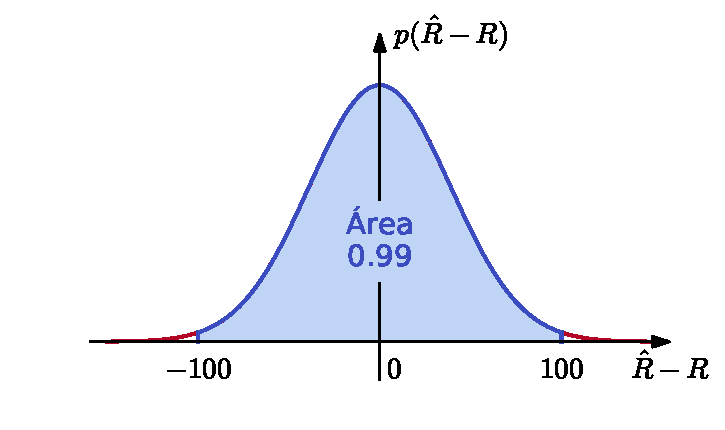
\includegraphics[width=\textwidth]{figuras/problem_1_1.pdf}
  \end{minipage}\hfill
  \begin{minipage}[c]{0.35\textwidth}
    \caption{
       Densidad de probabilidad de la variable aleatoria \(\hat{R}-R\sim\mathcal{N}\left(0,\,\sigma^2_{\hat{\tau}_0}c^2/4\right)\). Se quiere determinar \(\sigma_{\hat{\tau}_0}\) de forma que \(\Pr\left\{|\hat{R}-R|\leq100\right\}\geq 0.99\).
    } \label{fig:problem_1_1}
  \end{minipage}
\end{figure}
Dividiendo entre la desviación estándar de \(\hat{R}\) se tiene que
\[
 \Pr\left\{-\frac{100}{\left(\dfrac{\sigma_{\hat{\tau}_0}c}{2}\right)}\leq\frac{\hat{R}-R}{\left(\dfrac{\sigma_{\hat{\tau}_0}c}{2}\right)}\leq\frac{100}{\left(\dfrac{\sigma_{\hat{\tau}_0}c}{2}\right)}\right\}\geq 0.99.
\]
De esta forma, la variable aleatoria tiene distribución normal estandarizada \(\mathcal{N}(0,\,1)\) y es posible emplear las tablas, como por ejemplo, la tabla de la distribución normal acumulada desde la media\footnote{\url{https://en.wikipedia.org/wiki/Standard_normal_table\#Cumulative_from_mean_(0_to_Z)}}. Teniendo en cuenta que la densidad de probabilidad estándar es una función simétrica, la expresión es equivalente a
\[
 \Pr\left\{0\leq\frac{\hat{R}-R}{\left(\dfrac{\sigma_{\hat{\tau}_0}c}{2}\right)}\leq\frac{100}{\left(\dfrac{\sigma_{\hat{\tau}_0}c}{2}\right)}\right\}\geq \frac{0.99}{2}=0.495,
\]
y recurriendo a la tabla, se obtiene que 
\[
 \frac{100}{\left(\dfrac{\sigma_{\hat{\tau}_0}c}{2}\right)}\geq 2.58.
\]
Finalmente, despejando se llega a que
\[
 \sigma_{\hat{\tau}_0}\leq\frac{200}{2.58c}=\frac{200}{2.58\times3\times10^8}\SI{}{\s}\approx 2.6\times10^{-7}\SI{}{\s}=\SI{0.26}{\micro\s}.
\]

\subsection{Problema 2}

Un parámetro desconocido \(\theta\) influencia en el resultado de un experimento que se modela mediante la variable aleatoria \(x\). La PDF de \(x\) es
\[
 p(x;\,\theta)=\frac{1}{\sqrt{2\pi}}\exp\left[-\frac{1}{2}(x-\theta)^2\right].
\]
Se realizan una serie de experimentos, y se observa que \(x\) está siempre en el intervalo \([97,\,103]\). En base a ello, el investigador concluye que \(\theta\) debe ser 100. ¿Es correcta esta afirmación?

\paragraph{Solución} Considérese el caso en que \(\theta\) es efectivamente 100. De esta forma,
\[
 p(x;\,\theta)=\frac{1}{\sqrt{2\pi}}\exp\left[-\frac{1}{2}(x-100)^2\right].
\]
La probabilidad de que \(x\) esté en el intervalo \([97,\,103]\) es
\begin{align*}
 \Pr\left\{97\leq x\leq103\,|\,\theta=100\right\}&\overset{(a)}{=}\Pr\left\{\frac{97-\mu}{\sigma}\leq \frac{x-\mu}{\sigma}\leq\frac{103-\mu}{\sigma}\,\Big|\,\theta=100\right\}\\
  &\overset{(b)}{=}\Pr\left\{-3\leq\frac{x-\mu}{\sigma}\leq 3\right\}\\
  &\overset{(c)}{=}2\Pr\left\{0\leq\frac{x-\mu}{\sigma}\leq 3\right\}\\
  &\overset{(d)}{=}2\times0.49865,
\end{align*}
donde en \((a)\) se normalizó la variable aleatoria \(x\) como \((x-\mu)/\sigma\sim\mathcal{N}(0,\,1)\), siendo \(\mu\) y \(\sigma\) la media y la desviación estándar de \(x\) respectivamente, en \((b)\) se consideró que \(\mu=\theta=100\) y \(\sigma=1\), en \((c)\) que la densidad de probabilidad normal es simétrica y el valor en \((d)\) se obtiene de la tabla de la distribución normal acumulada desde la media. Se concluye que
\[
 \Pr\left\{97\leq x\leq103\,|\,\theta=100\right\}=0.9973
\]
en un único experimento, por lo que el valor \(\theta=100\) es altamente probable.

Considérese el caso en que el valor verdadero de \(\theta\) es por ejemplo 99. En este caso, se cumple que
\begin{align*}
 \Pr\left\{97\leq x\leq103\,|\,\theta=99\right\}&=\Pr\left\{\frac{97-\mu}{\sigma}\leq \frac{x-\mu}{\sigma}\leq\frac{103-\mu}{\sigma}\,\Big|\,\theta=99\right\}\\
  &\overset{(a)}{=}\Pr\left\{-2\leq\frac{x-\mu}{\sigma}\leq 4\right\}\\
  &=\Pr\left\{0\leq\frac{x-\mu}{\sigma}\leq 2\right\}+\Pr\left\{0\leq\frac{x-\mu}{\sigma}\leq 4\right\}\\
  &=0.47725+0.49997,
\end{align*}
donde en \((a)\) se consideró que \(\mu=\theta=99\) y \(\sigma=1\),
resultando en
\[
 \Pr\left\{97\leq x\leq103\,|\,\theta=99\right\}=0.97722
\]
en un único experimento. Este razonamiento muestra que la obtención de \(x\) en el intervalo  \([97,\,103]\) en un único experimento tiene probabilidad muy alta  tanto si \(\theta=100\) o \(\theta=99\), y por lo tanto, el valor verdadero de \(\theta\) podría ser cualquiera de ellos. Se concluye que la afirmación de que \(\theta\) debe ser 100 no es correcta.

Supóngase ahora que el experimento se realiza 100 veces. Asumiendo que los experimentos son independientes, se tiene que
\begin{align*}
 \Pr\{x\in[97,\,103]\textrm{ en los 100 experimentos}\,|\,\theta=100\}&=\left(\Pr\left\{97\leq x\leq103\,|\,\theta=100\right\}\right)^{100}\\
  &=0.9973^{100}\\
  &\approx0.76,
\end{align*}
mientras que
\begin{align*}
 \Pr\{x\in[97,\,103]\textrm{ en los 100 experimentos}\,|\,\theta=99\}&=\left(\Pr\left\{97\leq x\leq103\,|\,\theta=99\right\}\right)^{100}\\
  &=0.97722^{100}\\
  &\approx0.1.
\end{align*}
Como la probabilidad de obtener \(x\) en el intervalo  \([97,\,103]\) en los 100 experimentos es considerablemente mas alta si \(\theta=100\) que si \(\theta=99\), podría afirmarse con mayor certeza que \(\theta\) debe ser 100.

\subsection{Problema 3}\label{sec:problem_1_3}

Sea \(\x=\theta+\w\), donde \(\w\) es una variable aleatoria con PDF \(p_w(w)\). Si \(\theta\) es un parámetro determinístico, encontrar la PDF de \(\x\) en términos de \(p_w\), la cual se denotará \(p(x;\,\theta)\). Luego, asumiendo que \(\theta\) es una variable aleatoria independiente de \(\w\), encontrar la PDF condicional \(p(x\,|\,\theta)\). Finalmente, determinar \(p(x|\theta)\) sin asumir que \(\theta\) y \(\w\) son independientes. ¿Qué se puede decir respecto a \(p(x;\,\theta)\) y \(p(x\,|\,\theta)\)?\footnote{En este problema, las letras en negrita representan variables aleatorias escalares, a diferencia del resto del documento, en donde las letras en negrita representan variables alatorias vectoriales.}

\paragraph{Solución} En el caso en que \(\theta\) es un parámetro determinístico, la PDF de \(\x\) es la PDF de \(\w\) desplazada una cantidad \(\theta\) hacia la derecha, es decir,
\[
 p(x;\,\theta)=p_w(x-\theta).
\]

Para encontrar \(p(x\,|\,\theta)\) en el caso en que \(\bm{\theta}\) y \(\w\) son variables aleatorias independientes, puede partirse de la distribución de probabilidad condicional,
\begin{align*}
 F_{x|\theta}(x\,|\,\theta)&=\Pr\{\x\leq x\,|\,\bm{\theta}=\theta\}\\
   &=\Pr\{\bm{\theta}+\w\leq x\,|\,\bm{\theta}=\theta\}\\
   &\overset{(a)}{=}\Pr\{\w\leq x-\theta\,|\,\bm{\theta}=\theta\}\\
   &\overset{(b)}{=}\frac{\Pr\{\w\leq x-\theta,\,\bm{\theta}=\theta\}}{\Pr\{\bm{\theta}=\theta\}}\\
   &\overset{(c)}{=}\frac{\Pr\{\w\leq x-\theta\}\Pr\{\bm{\theta}=\theta\}}{\Pr\{\bm{\theta}=\theta\}}\\
   &=\Pr\{\w\leq x-\theta\}\\
   &=F_w(x-\theta),
\end{align*}
donde en \((a)\) se sustituyó la variable aleatoria \(\bm{\theta}\) por el valor dado por el condicional, en \((b)\) se aplicó la definición de probabilidad condicional y en \((c)\) se consideró que las variables aleatorias \(\w\) y \(\bm{\theta}\) son independientes. Derivando respecto a \(x\), se obtiene la PDF buscada,
\[
 p(x\,|\,\theta)=p_w(x-\theta).
\]
Este razonamiento no es completamente formal debido a que el evento \(\{\bm{\theta}=\theta\}\) tiene en general probabilidad nula. Para formalizarlo, habría que considerar el evento \(\{\theta\leq\bm{\theta}\leq\theta+\Delta\theta\}\) y tomar el límite \(\Delta\theta\to0\). El mismo razonamiento puede hacerse directamente a partir de las PDF, pero se eligió incluirlo por hacerlo mas explícito. Usando las densidades, la deducción es como sigue,
\begin{align*}
 p(x\,|\,\theta)=\frac{p_{x\theta}(x,\,\theta)}{p(\theta)}=\frac{p_{w\theta}(x-\theta,\,\theta)}{p(\theta)}=\frac{p_w(x-\theta)p(\theta)}{p(\theta)}=p_w(x-\theta).
\end{align*}
Se concluye que en el caso en que \(\theta\) y \(\w\) son independientes,
\[
 p(x;\,\theta)=p(x\,|\,\theta).
\]

Se considera a continuación el caso en que \(\theta\) y \(\w\) no son independientes. Nuevamente, partiendo de la distribución condicional, se cumple que
\begin{align*}
 F_{x|\theta}(x\,|\,\theta)&=\Pr\{\x\leq x\,|\,\bm{\theta}=\theta\}\\
   &=\Pr\{\bm{\theta}+\w\leq x\,|\,\bm{\theta}=\theta\}\\
   &=\Pr\{\w\leq x-\theta\,|\,\bm{\theta}=\theta\}\\
   &=F_{w|\theta}(x-\theta\,|\,\theta),
\end{align*}
y derivando respecto a \(x\) se llega a que
\[
 p(x\,|\,\theta)=p_{w|\theta}(x-\theta\,|\,\theta),
\]
que en general no es igual a \(p(x;\,\theta)\).

\subsection{Problema 4}\label{sec:problema_1_4}

Se quiere estimar el valor \(A\) del nivel de corriente continua (\emph{direct current}, DC) en ruido blanco gaussiano (\emph{white gaussian noise}, WGN),
\[
 x[n]=A+w[n],\qquad n=0,\,1,\dots,\,N-1,
\]
donde \(w[n]\) es no correlacionado con media nula, y cada muestra tiene varianza \(\sigma^2=1\). Se consideran los dos estimadores
\begin{align*}
 \hat{A}&=\frac{1}{N}\sum_{n=0}^{N-1}x[n]\\
 \check{A}&=\frac{1}{N+2}\left(2x[0]+\sum_{n=1}^{N-2}x[n]+2x[N-1]\right)
\end{align*}
¿Cual de los dos es mejor? La respuesta anterior, ¿depende del valor de \(A\)?

\paragraph{Solución} Se comenzará analizando el sesgo de ambos estimadores. Para el estimador \(\hat{A}\) se cumple que
\begin{equation}\label{eq:sample_mean_mean}
 E(\hat{A})=E\left(\frac{1}{N}\sum_{n=0}^{N-1}x[n]\right)=\frac{1}{N}\sum_{n=0}^{N-1}E(x[n])=\frac{1}{N}\sum_{n=0}^{N-1}A=\frac{1}{N}NA=A,
\end{equation}
y para el estimador \(\check{A}\) se tiene que
\begin{align*}
 E(\check{A})&=\frac{1}{N+2}\left[2E(x[0])+\sum_{n=1}^{N-2}E(x[n])+2E(x[N-1])\right]\\
   &=\frac{1}{N+2}\left(2A+\sum_{n=1}^{N-2}A+2A\right)\\
   &=\frac{1}{N+2}\left(2A+(N-2)A+2A\right)\\
   &=\frac{1}{N+2}(N+2)A\\
   &=A.
\end{align*}
Se concluye que ambos estimadores son insesgados. Teniendo esto en cuenta, el mejor estimador es el de menor varianza. 
La varianza del estimador \(\hat{A}\) es
\begin{align}\label{eq:sample_mean_variance}
 \var(\hat{A})&=\var\left(\frac{1}{N}\sum_{n=0}^{N-1}x[n]\right)\nonumber\\
    &\overset{(a)}{=}\frac{1}{N^2}\sum_{n=0}^{N-1}\var(x[n])\nonumber\\
    &\overset{(b)}{=}\frac{1}{N^2}\sum_{n=0}^{N-1}\var(w[n])\nonumber\\
    &=\frac{1}{N^2}\sum_{n=0}^{N-1}\sigma^2\nonumber\\
    &=\frac{1}{N^2}N\sigma^2\nonumber\\
    &=\frac{\sigma^2}{N},
\end{align}
donde en \((a)\) se empleó que las variables aleatorias \(x[n]\) son independientes debido a que las variables aleatorias \(w[n]\) son independientes y que si \(a\) y \(b\) son constantes y \(X\) es una variable aleatoria se cumple que \(\var(aX+b)=a^2\var(X)\). Esta propiedad de la varianza también se empleó en \((b)\). Teniendo en cuenta que en este caso \(\sigma^2=1\), se obtiene que
\[
 \var(\hat{A})=\frac{1}{N}.
\]
La varianza de \(\check{A}\) es
\begin{align*}
 \var(\check{A})&=\frac{1}{(N+2)^2}\left[4\var(x[0])+\sum_{n=1}^{N-2}\var(x[n])+4\var(x[N-1])\right]\\
   &=\frac{1}{(N+2)^2}\left[4\var(w[0])+(N-2)\var(w[n])+4\var(w[N-1])\right]\\
   &=\frac{1}{(N+2)^2}\left[4+(N-2)+4\right]\\
   &=\frac{N+6}{(N+2)^2}.
\end{align*}
Notando que 
\begin{align*}
 \var(\check{A})-\var(\hat{A})&=\frac{N+6}{(N+2)^2}-\frac{1}{N}\\
   &=\frac{(N+6)N-(N+2)^2}{N(N+2)^2}\\
   &=\frac{(N^2+6N)-(N^2+4N+4)}{N(N+2)^2}\\
   &=\frac{2N-4}{N(N+2)^2}\\
   &>0\qquad{\textrm{si }N\geq3},
\end{align*}
se concluye que el estimador \(\hat{A}\) es mejor por tener menor varianza. Como la varianza de los estimadores es independiente de \(A\), el desempeño del estimador \(\hat{A}\) es mejor para todo valor de \(A\).

\subsection{Problema 5} 

Para los mismos datos del problema anterior se propone el siguiente estimador:
\[\def\arraystretch{2}
 \hat{A}=
 \left\{\begin{array}{ll}
  x[0], &  \textrm{si }\dfrac{A}{\sigma^2}=A^2>1000\\
  \dfrac{1}{N}\sum\limits_{n=0}^{N-1}x[n], &  \textrm{si }\dfrac{A}{\sigma^2}=A^2\leq1000.
 \end{array}\right.
\]
La fundamentación de este estimador es que para relaciones señal a ruido (\emph{signal-to-noise ratio}, SNR) suficientemente altas, no se necesita reducir el efecto del ruido mediante el promediado y de esta forma, se reduce el costo computacional. Comentar sobre este enfoque.

\paragraph{Solución} \(\hat{A}\) no es un estimador, ya que para implementarlo se requiere el conocimiento de \(A\) para calcular la SNR \(A/\sigma^2\).

\chapter{Estimación insesgada de varianza mínima}

\section{Problemas}

\subsection{Problema 1}\label{sec:problema_2_1} 

Se observan los datos \(\{x[0],\,x[1],\dots,x[N-1]\}\), donde las muestras \(x[n]\) son independientes e idénticamente distribuidas (IID) como \(\mathcal{N}(0,\,\sigma^2)\). Se quiere estimar la varianza \(\sigma^2\) como
\[
 \hat{\sigma^2}=\frac{1}{N}\sum_{n=0}^{N-1}x^2[n].
\]
¿Es este estimador insesgado? Calcular la varianza de \(\hat{\sigma^2}\) e indicar que ocurre cuando \(N\to\infty\).

\paragraph{Solución} Para verificar si el estimador es insesgado hay que confirmar que \(E(\hat{\sigma^2})=\sigma^2\). En este caso, se cumple que
\[
 E(\hat{\sigma^2})=\frac{1}{N}\sum_{n=0}^{N-1}E(x^2[n])
   \overset{(a)}{=}\frac{1}{N}\sum_{n=0}^{N-1}\sigma^2
   =\frac{1}{N}N\sigma^2
   =\sigma^2,
\]
donde en \((a)\) se tuvo en cuenta que \(\sigma^2\triangleq\var(x[n])=E(x^2[n])-E^2(x[n])=E(x^2[n])\) ya que los \(x[n]\) tienen media nula. Se concluye que \(\hat{\sigma^2}\) es insesgado.

La varianza de \(\hat{\sigma^2}\) es
\begin{align*}
 \var(\hat{\sigma^2})&=\frac{1}{N^2}\sum_{n=0}^{N-1}\var(x^2[n])\\
   &\overset{(a)}{=}\frac{1}{N^2}\sum_{n=0}^{N-1}2\sigma^4\\
   &=\frac{1}{N^2}2N\sigma^4\\
   &=\frac{2\sigma^4}{N},
\end{align*}
donde en \((a)\) se tuvo en cuenta que
\[
 \var(x^2[n])=E(x^4[n])-E^2(x^2[n])=3\sigma^4-\sigma^4=2\sigma^4,
\]
ya que los momentos centrales segundo y cuarto de una variable aleatoria normal son \(\sigma^2\) y \(3\sigma^4\) respectivamente (ver el capítulo 5 de  \cite{papoulis2002probability}, por ejemplo). Además, cuando \(N\to\infty\), se cumple que
\[
 \lim_{N\to\infty}\var(\hat{\sigma^2})=\lim_{N\to\infty}\frac{2\sigma^4}{N}=0.
\]
Como el estimador es insesgado, esto implica que la PDF de los datos se concentra cada vez mas en torno al valor verdadero del parámetro a medida que se incrementa la cantidad de datos. Un estimador con esta característica se llama \emph{consistente}, como se verá mas detalladamente en el problema de la sección \ref{sec:problem_2_8}.

\subsection{Problema 2}\label{sec:problem_2_2}

Se consideran los datos \(\{x[0],\,x[1],\dots,x[N-1]\}\), donde cada muestra tiene distribución \(\mathcal{U}(0,\,\theta)\) y son IID. Encontrar un estimador de \(\theta\). El rango de \(\theta\) es \(0<\theta<\infty\).

\paragraph{Solución} Una posibilidad es buscar un estimador a partir de la media muestral \(\bar{x}\). Puede verse que \(E(x[n])=\theta/2\),
\[
 E(x[n])=\int_{-\infty}^{\infty}xp(x;\,\theta)\,dx=\frac{1}{\theta}\int_{0}^{\theta}x\,dx
  =\frac{1}{\theta}\left(\frac{x^2}{2}\bigg|_{0}^{\theta}\right)
  =\frac{1}{\theta}\left(\frac{\theta^2}{2}-0\right)
  =\frac{\theta}{2}.
\]
Por lo tanto, la esperanza de la media muestral también es \(\theta/2\),
\[
 E(\bar{x})=\frac{1}{N}\sum_{n=0}^{N-1}E(x[n])=\frac{1}{N}\sum_{n=0}^{N-1}\frac{\theta}{2}
  =\frac{1}{N}N\frac{\theta}{2}=\frac{\theta}{2}.
\]
Como \(2E(\bar{x})=\theta\), un estimador insesgado de \(\theta\) es
\[
 \hat{\theta}=2\bar{x}.
\]

\subsection{Problema 3}\label{sec:problem_2_3}

Considérese las observaciones
\[
 x[n]=A+w[n],\qquad n=0,\,1,\dots,\,N-1,
\]
donde \(A\) es el parámetro a estimar y \(w[n]\) es WGN. El parámetro \(A\) puede tomar cualquier valor en el intervalo \(-\infty<A<\infty\). Un estimador razonable de \(A\) es la media muestral,
\[
 \hat{A}=\frac{1}{N}\sum_{n=0}^{N-1}x[n].
\]
Demostrar que la PDF de \(\hat{A}\) es \(\mathcal{N}(A,\,\sigma^2/N)\).

\paragraph{Solución}

\(\hat{A}\) es una variable aleatoria gaussiana por ser una combinación lineal de variables aleatorias gaussianas (ver los capítulos 6 y 7 de \cite{papoulis2002probability}), por lo que para determinar su PDF basta con calcular la media y la varianza. La media y la varianza de \(\hat{A}\) ya se calcularon en la sección \ref{sec:problema_1_4} (ecuaciones \ref{eq:sample_mean_mean} y \ref{eq:sample_mean_variance} respectivamente), y son
\[
 E(\hat{A})=A\qquad\qquad \var(\hat{A})=\frac{\sigma^2}{N}.
\]
Se concluye que \(\hat{A}\sim\mathcal{N}(A,\,\sigma^2/N)\).

\subsection{Problema 4} 

La tasa del latido del corazón de un paciente se mide automáticamente con una computadora cada 100 ms. En 1 s las medidas \(\{\hat{h}_1,\,\hat{h}_2,\dots,\,\hat{h}_{10}\}\) se promedian para obtener \(\hat{h}\). Si \(E(\hat{h}_i)=\alpha h\) para alguna constante \(\alpha\) y \(\var(\hat{h}_i)=1\) para cada \(i\), determinar si el promediado mejora el estimador cuando \(\alpha=1\) y \(\alpha=1/2\). Asumir que las medidas son no correlacionadas.

\paragraph{Solución} 

Se comenzará estudiando el sesgo de \(\hat{h}\) en función del parámetro \(\alpha\). Como
\[
 \hat{h}=\frac{1}{10}\sum_{i=1}^{10}\hat{h}_i,
\]
la esperanza de \(\hat{h}\) es
\[
 E(\hat{h})=\frac{1}{10}\sum_{i=1}^{10}E(\hat{h}_i)=\frac{1}{10}\sum_{i=1}^{10}\alpha h
  =\frac{1}{10}10\alpha h=\alpha h.
\]
Se concluye que el estimador \(\hat{h}\) es insesgado solo si \(\alpha=1\). Además, la varianza de \(\hat{h}\) es
\[
 \var(\hat{h})=\var\left(\frac{1}{10}\sum_{i=1}^{10}\hat{h}_i\right)
 \overset{(a)}{=}\frac{1}{10^2}\sum_{i=1}^{10}\var(\hat{h}_i)
 =\frac{1}{100}\sum_{i=1}^{10}1
 =\frac{1}{100}10=\frac{1}{10},
\]
donde en \((a)\) se consideró que las medidas \(\hat{h}_i\) son no correlacionadas.
Este resultado indica que el promediado de las 10 medidas reduce la varianza 1/10 respecto a una medida individual.
\begin{figure}[!htb]
\begin{center}
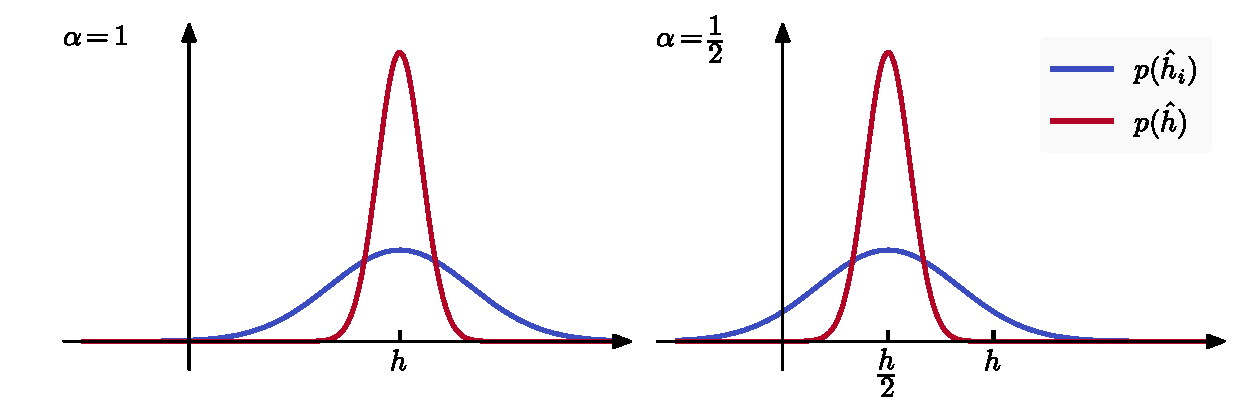
\includegraphics[width=0.9\textwidth]{figuras/problem_2_4.pdf}
\caption{\label{fig:problem_2_4} PDF de una medida individual \(\hat{h}_i\) y de las medidas promediadas \(\hat{h}\) para \(\alpha=1\) y \(\alpha=1/2\) en el caso gaussiano.}
\end{center}
\end{figure}
En la figura \ref{fig:problem_2_4} se muestran las PDF en el caso gaussiano. Con \(\alpha=1/2\), el promediado hace que la PDF esté mas concentrada en torno al valor incorrecto de \(h\), haciendo que la probabilidad de que \(\hat{h}\) esté cerca de \(h\) se reduzca. En el caso con \(\alpha=1\) en que el estimador es insesgado, el promediado es favorable, ya que incrementa la probabilidad de que \(\hat{h}\) esté cercano al valor verdadero \(h\). 

\subsection{Problema 5} 

Dos muestras \(\{x[0],\,x[1]\}\) son observadas independientemente de una distribución \(\mathcal{N}(0,\,\sigma^2)\). El estimador
\[
 \hat{\sigma^2}=\frac{1}{2}(x^2[0]+x^2[1])
\]
es insesgado. Encontrar la PDF de \(\hat{\sigma^2}\) para determinar si es simétrica respecto a \(\sigma^2\).

\paragraph{Solución} En el problema de la sección \ref{sec:problema_2_1} se demostró que el estimador \(\hat{\sigma^2}\) es insesgado. 
Por otro lado, puede demostrarse que si \(x\) es una variable aleatoria \(\mathcal{N}(0,\,1)\), \(x^2\) es una variable aleatoria chi-cuadrado con un grado de liberad (ver el capítulo 5 de \cite{papoulis2002probability}), es decir, \(x^2\sim\chi^2(1)\). Además, se cumple que si
\[
 z=x_1^2+\dots+x_n^2
\]
donde \(x_i,\,i=1,\dots,\,n\), son variables aleatorias \(\mathcal{N}(0,\,1)\) independientes, la variable aleatoria \(z\) es chi-cuadrado con \(n\) grados de libertad (ver el capítulo 7 de \cite{papoulis2002probability}). La PDF de una variable aleatoria \(z\sim\chi^2(n)\) es
\begin{equation}\label{eq:pdf_chi_square}
 \def\arraystretch{2.0}
 p(z)=
 \left\{\begin{array}{ll}
  \dfrac{z^{n/2-1}}{2^{n/2}\Gamma(n/2)} e^{-z/2}, & z\geq 0\\
  0, & \textrm{en otro caso}
 \end{array}, \right.
\end{equation}
donde \(\Gamma(\alpha)\) es la función gama, definida como
\begin{equation}\label{eq:gamma_function}
 \Gamma(\alpha)=\int_{0}^{\infty}z^{\alpha-1}e^{-z}\,dz.
\end{equation}
Puede demostrarse que si \(n\) es un número entero positivo, se cumple que \(\Gamma(n)=(n-1)!\) (ver el capítulo 4 de \cite{papoulis2002probability}).
Como
\[
 x[n]\sim\mathcal{N}(0,\,\sigma^2)\qquad\Rightarrow\qquad\frac{x[n]}{\sigma}\sim\mathcal{N}(0,\,1)\qquad\Rightarrow\qquad\frac{x^2[n]}{\sigma^2}\sim\chi^2(1),
\]
y por lo tanto,
\[
 y=\frac{1}{\sigma^2}(x^2[0]+x^2[1])\sim\chi^2(2).
\]
De esta forma, sustituyendo \(n=2\) en la ecuación \ref{eq:pdf_chi_square}, la PDF \(p(y)\) de la variable aleatoria \(y\) es
\[
 \def\arraystretch{2.0}
 p(y)=
 \left\{\begin{array}{ll}
  \dfrac{e^{-y/2}}{2\Gamma(1)}, & y\geq 0\\
  0, & \textrm{en otro caso}
 \end{array}, \right.
\]
y sustituyendo \(\alpha=1\) en la función gamma (ecuación \ref{eq:gamma_function}) se tiene que
\[
 \Gamma(1)=\int_{0}^{\infty}e^{-y}\,dy=-e^{-y}\bigg|_{0}^{\infty}=-(0-1)=1.
\]
Se concluye que 
\[
 p(y)=\frac{e^{-y/2}}{2},\qquad y\geq 0.
\]
Teniendo en cuenta que
\[
 \hat{\sigma^2}=\frac{\sigma^2}{2}y,
\]
la PDF de \(\hat{\sigma^2}\) puede calcularse a partir de la PDF de \(y\) mediante el teorema fundamental de transformaciones de variables aleatorias (ver el capítulo 5 de \cite{papoulis2002probability}), que indica que si \(x\) es una variable aleatoria con PDF \(p_x(x)\), la PDF \(p_y(y)\) de la variable aleatoria \(y=g(x)\) es
\begin{equation}\label{eq:pdf_parameters_transformation}
 p_y(y)=\sum_{i}\frac{p_x(x_i)}{|g'(x_i)|}, 
\end{equation}
donde \(x_i\) son las raíces de \(y=g(x)\) para un valor específico de \(y\), es decir, \(x_i=g^{-1}(y)\) para el valor de \(y\) que se quiere calcular la PDF. Como en este caso la transformación es inyectiva, con
\[
 y=\frac{2}{\sigma^2}\hat{\sigma^2},
\]
y la derivada de la transformación es \(\hat{\sigma^2}'(y)=\sigma^2/2\), se obtiene que
\[
 p(\hat{\sigma^2})=\frac{p(2\hat{\sigma^2}/\sigma^2)}{\sigma^2/2}=\frac{e^{-\hat{\sigma^2}/\sigma^2}}{\sigma^2},\qquad \hat{\sigma^2}\geq 0,
\]
es decir, \(\hat{\sigma^2}\) tiene PDF exponencial con parámetro \(\lambda=1/\sigma^2\).
\begin{figure}[!htb]
  \begin{minipage}[c]{0.55\textwidth}
    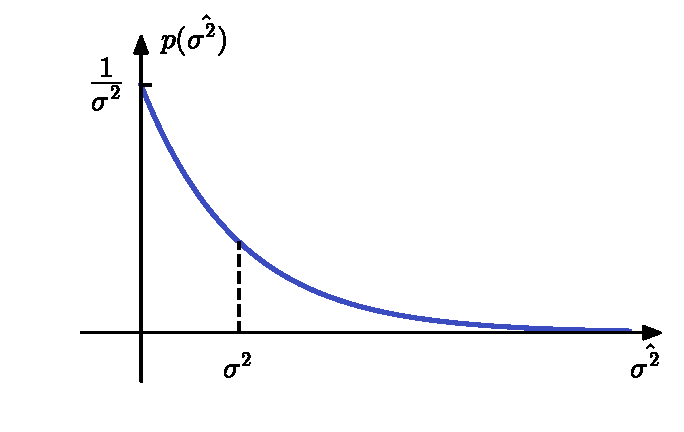
\includegraphics[width=\textwidth]{figuras/problem_2_5.pdf}
  \end{minipage}\hfill
  \begin{minipage}[c]{0.35\textwidth}
    \caption{
       Densidad de probabilidad de la variable aleatoria \(\hat{\sigma^2}\).
    } \label{fig:problem_2_5}
  \end{minipage}
\end{figure}
Claramente, la PDF no es simétrica  respecto a la media \(\sigma^2\), como se muestra en la figura \ref{fig:problem_2_5}.

\subsection{Problema 6}\label{sec:problem_2_6}

Para el problema de estimación del nivel de DC en WGN (ver sección \ref{sec:problema_1_4}) se propone el siguiente estimador mas genérico:
\[
 \hat{A}=\sum_{n=0}^{N-1}a_nx[n].
\]
Encontrar los valores de los \(a_n\) de forma que el estimador sea insesgado y minimicen la varianza. Sugerencia: usar multiplicadores de Lagrange usando la condición de no sesgo como la ecuación de restricción.

\paragraph{Solución} Para encontrar los puntos estacionarios de una función \(f(x)\) sujeto a las condiciones de igualdad \(g_i(x)=0\), \(i=1,\dots,\,m\), hay que encontrar los puntos estacionarios de la función Lagrangiana\footnote{Ver \url{https://en.wikipedia.org/wiki/Lagrange_multiplier}}, dada por
\[
 \mathcal{L}(x,\,\lambda)=f(x)-\sum _{i=1}^{m}\lambda_{i}g_{i}(x).
\]
La función a minimizar es la varianza de \(\hat{A}\),
\[
 \var(\hat{A})=\sum_{n=0}^{N-1}a^2_n\var(x[n])=\sigma^2\sum_{n=0}^{N-1}a^2_n,
\]
y la restricción es que \(\hat{A}\) sea insesgado es
\[
 E(\hat{A})=\sum_{n=0}^{N-1}a_nE(x[n])=A\sum_{n=0}^{N-1}a_n=A,
\]
donde la última igualdad es la condición de insesgado, y resulta en
\[
 \sum_{n=0}^{N-1}a_n=1.
\]
Por lo tanto, la función Lagrangiana resulta en este caso en
\[
 \mathcal{L}(a_0,\dots,\,a_{N-1},\,\lambda)=\sigma^2\sum_{n=0}^{N-1}a^2_n-\lambda\left(\sum_{n=0}^{N-1}a_n-1\right).
\]
Los puntos estacionarios de \(\mathcal{L}(a_0,\dots,\,a_{N-1},\,\lambda)\) se obtienen derivando respecto a los \(a_i\), \(i=0,\dots,\,N-1\), igualando a 0 y resolviendo el sistema de \(N\) ecuaciones con \( N\) incógnitas,
\begin{equation}\label{eq:problem_2_6_coefs}
 \frac{\partial\mathcal{L}(a_0,\dots,\,a_{N-1},\,\lambda)}{\partial a_i}=2\sigma^2a_i-\lambda=0\qquad\Rightarrow\qquad a_i=\frac{\lambda}{2\sigma^2},\qquad i=0,\dots,\,N-1.
\end{equation}
Esto indica que los \(a_i\) tienen todos el mismo valor.
Sustituyendo los resultados en la ecuación de la restricción, se obtiene el valor de \(\lambda\),
\[
 \sum_{n=0}^{N-1}a_n=\sum_{n=0}^{N-1}\frac{\lambda}{2\sigma^2}=\frac{N\lambda}{2\sigma^2}=1\qquad\Rightarrow\qquad \lambda=\frac{2\sigma^2}{N}
\]
y sustituyendo el valor de \(\lambda\) en las ecuaciones \ref{eq:problem_2_6_coefs} de los coeficientes se llega a que
\[
 a_i=\frac{1}{N},\qquad i=0,\dots,\,N-1.
\]
Se concluye que el estimador \(\hat{A}\) insesgado que minimiza la varianza es la media muestral.

\subsection{Problema 7}

Se proponen dos estimadores insesgados cuyas varianzas cumplen que \(\var(\hat{\theta})<\var(\check{\theta})\). Si ambos estimadores son gaussianos, demostrar que
\[
 \Pr\big\{|\hat{\theta}-\theta|>\epsilon\big\}<
 \Pr\big\{|\check{\theta}-\theta|>\epsilon\big\}
\]
para todo \(\epsilon>0\). Este resultado indica que el estimador de menor varianza es mejor ya que su PDF está mas concentrada en torno al valor verdadero.

\paragraph{Solución} Como los estimadores son insesgados, se cumple que \(E(\hat{\theta})=E(\check{\theta})=\theta\), y por lo tanto, \(\hat{\theta}-\theta\sim\mathcal{N}(0,\,\var(\hat{\theta}))\) y \(\check{\theta}-\theta\sim\mathcal{N}(0,\,\var(\check{\theta}))\). De esta forma,
\begin{align*}
 \Pr\big\{|\hat{\theta}-\theta|>\epsilon\big\}&=\Pr\big\{\hat{\theta}-\theta>\epsilon\big\}+\Pr\big\{\hat{\theta}-\theta<-\epsilon\big\}\\
  &=2\Pr\big\{\hat{\theta}-\theta>\epsilon\big\}\\
  &=2\Pr\left\{\frac{\hat{\theta}-\theta}{\sqrt{\var(\hat{\theta})}}>\frac{\epsilon}{\sqrt{\var(\hat{\theta})}}\right\},\qquad\textrm{con}\quad\frac{\hat{\theta}-\theta}{\sqrt{\var(\hat{\theta})}}\sim\mathcal{N}(0,\,1).
\end{align*}
Realizando el mismo razonamiento para \(\check{\theta}\), se obtiene que
\[
 \Pr\big\{|\check{\theta}-\theta|>\epsilon\big\}=2\Pr\left\{\frac{\check{\theta}-\theta}{\sqrt{\var(\check{\theta})}}>\frac{\epsilon}{\sqrt{\var(\check{\theta})}}\right\},\qquad\textrm{con}\quad\frac{\check{\theta}-\theta}{\sqrt{\var(\check{\theta})}}\sim\mathcal{N}(0,\,1).
\]

Considérese la distribución de probabilidad acumulada complementaria de una variable aleatoria normal estándar, definida como
\begin{equation}\label{eq:gaussian_complementary_cumulative}
 f(z)=\Pr\{Z>z\}=\frac{1}{\sqrt{2\pi}}\int_{z}^{\infty}e^{-t^2/2}\,dt.
\end{equation}
De esta forma,
\[
 \Pr\big\{|\hat{\theta}-\theta|>\epsilon\big\}=2f\left(\frac{\epsilon}{\sqrt{\var(\hat{\theta})}}\right)\qquad\textrm{y}\qquad
 \Pr\big\{|\check{\theta}-\theta|>\epsilon\big\}=2f\left(\frac{\epsilon}{\sqrt{\var(\check{\theta})}}\right).
\]
\(f(z)\) es una función decreciente con \(z\), y por lo tanto, como
\[
 \var(\hat{\theta})<\var(\check{\theta})\qquad\Rightarrow\qquad
 \frac{\epsilon}{\sqrt{\var(\hat{\theta})}}>\frac{\epsilon}{\sqrt{\var(\check{\theta})}}
\]
se cumple que
\[
 f\left(\frac{\epsilon}{\sqrt{\var(\hat{\theta})}}\right)<
 f\left(\frac{\epsilon}{\sqrt{\var(\check{\theta})}}\right),
\]
concluyendo que
\[
 \Pr\big\{|\hat{\theta}-\theta|>\epsilon\big\}<
 \Pr\big\{|\check{\theta}-\theta|>\epsilon\big\}.
\]
En la figura \ref{fig:problem_2_7} se muestran todas las PDF involucradas en el problema. Las áreas sombreadas son las probabilidades.
\begin{figure}[!htb]
\begin{center}
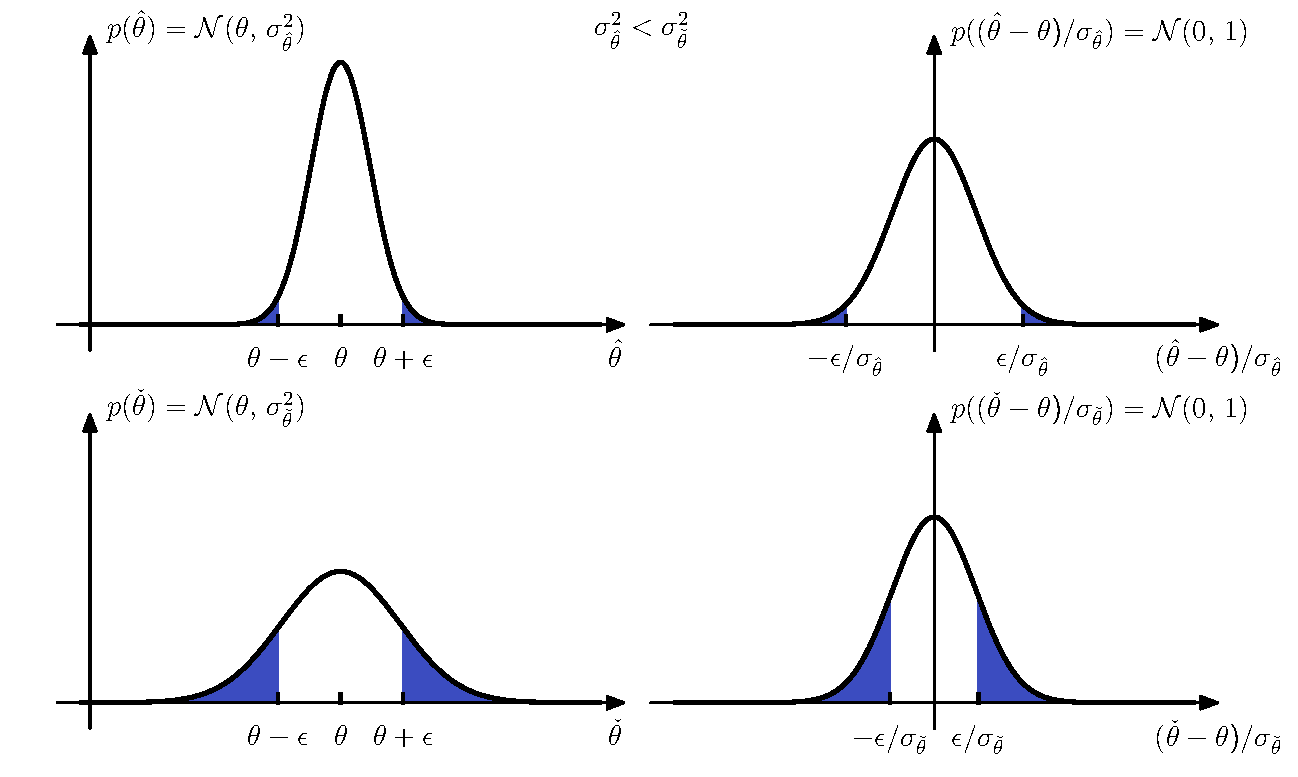
\includegraphics[width=0.95\textwidth]{figuras/problem_2_7.pdf}
\caption{\label{fig:problem_2_7} PDF y PDF normalizada de \(\hat{\theta}\) (arriba) y \(\check{\theta}\) (abajo). Las áreas sombreadas son \(\Pr\big\{|\hat{\theta}-\theta|>\epsilon\big\}\) y \(\Pr\big\{|\check{\theta}-\theta|>\epsilon\big\}\).}
\end{center}
\end{figure}

\subsection{Problema 8}\label{sec:problem_2_8}

Para el problema de estimación del nivel de DC en WGN, usar el resultado del problema de la sección \ref{sec:problem_2_3} para demostrar que \(\hat{A}\to A\) cuando \(N\to\infty\). Para hacerlo, demostrar que
\[
 \lim_{N\to\infty}\Pr\big\{|\hat{A}-A|>\epsilon\big\}=0
\]
para todo \(\epsilon>0\). En ese caso, se dice que el estimador \(\hat{A}\) es \emph{consistente}. Investigar que sucede si se emplea el estimador alternativo
\[
 \check{A}=\frac{1}{2N}\sum_{n=0}^{N-1}x[n].
\]

\paragraph{Solución} En el problema de la sección \ref{sec:problem_2_3}, se demostró que \(\hat{A}\sim\mathcal{N}(A,\,\sigma^2/N)\). Por lo tanto, siguiendo un razonamiento análogo al del problema anterior se tiene que
\[
 \Pr\big\{|\hat{A}-A|>\epsilon\big\}=2\Pr\big\{\hat{A}-A>\epsilon\big\}
 =2\Pr\left\{\frac{\hat{A}-A}{\sigma/\sqrt{N}}>\frac{\epsilon}{\sigma/\sqrt{N}}\right\}
 =2f\left(\frac{\epsilon}{\sigma/\sqrt{N}}\right),
\]
donde la función \(f\) es la distribución de probabilidad acumulada complementaria de una variable aleatoria normal estándar, definida en la ecuación \ref{eq:gaussian_complementary_cumulative}. Como
\[
 \forall\epsilon>0,\quad\lim_{N\to\infty}\frac{\epsilon}{\sigma/\sqrt{N}}=\infty\qquad\textrm{y además}\qquad \lim_{z\to\infty}f(z)=\lim_{z\to\infty}\frac{1}{\sqrt{2\pi}}\int_{z}^{\infty}e^{-t^2/2}\,dt=0,
\]
se concluye que
\begin{equation}\label{eq:sample_mean_consistency}
 \lim_{N\to\infty}\Pr\big\{|\hat{A}-A|>\epsilon\big\}=0\qquad\forall\epsilon>0.
\end{equation}
Esta ecuación es la definición de \emph{convergencia en probabilidad} de una variable aleatoria (ver el capítulo 7 de \cite{papoulis2002probability}), es decir, cuando se verifica la ecuación \ref{eq:sample_mean_consistency}, se dice que la variable aleatoria \(\hat{A}\) converge en probabilidad a la constante \(A\). Cuando el estimador de un parámetro converge en probabilidad al valor verdadero del parámetro, se dice que el estimador es \emph{consistente}.

En el caso del estimador alternativo \(\check{A}\), se cumple que
\[
 E(\check{A})=\frac{1}{2N}\sum_{n=0}^{N-1}E(x[n])=\frac{1}{2N}NA=\frac{A}{2},
\]
es decir, el estimador no es insesgado. Por otro lado, la varianza del estimador es
\[
 \var(\check{A})=\frac{1}{4N^2}\sum_{n=0}^{N-1}\var(x[n])=\frac{1}{4N^2}N\sigma^2=\frac{\sigma^2}{4N}.
\]
Se concluye que \(\check{A}\sim\mathcal{N}(A/2,\,\sigma^2/4N)\). Por lo tanto, 
\[
 \lim_{N\to\infty}\var(\check{A})=\lim_{N\to\infty}\frac{\sigma^2}{4N}=0,
\]
lo que implica que la PDF de \(\check{A}\) se concentra cada vez mas en torno a su media \(A/2\). De esta forma,
\[
 \lim_{N\to\infty}\Pr\big\{|\check{A}-A|>\epsilon\big\}=1
\]
para todo \(\epsilon\in(0,\,A/2)\), como se muestra en la figura \ref{fig:problem_2_8}. Por lo tanto, \(\check{A}\) no converge en probabilidad a \(A\), así que no es consistente.
\begin{figure}[!htb]
\begin{center}
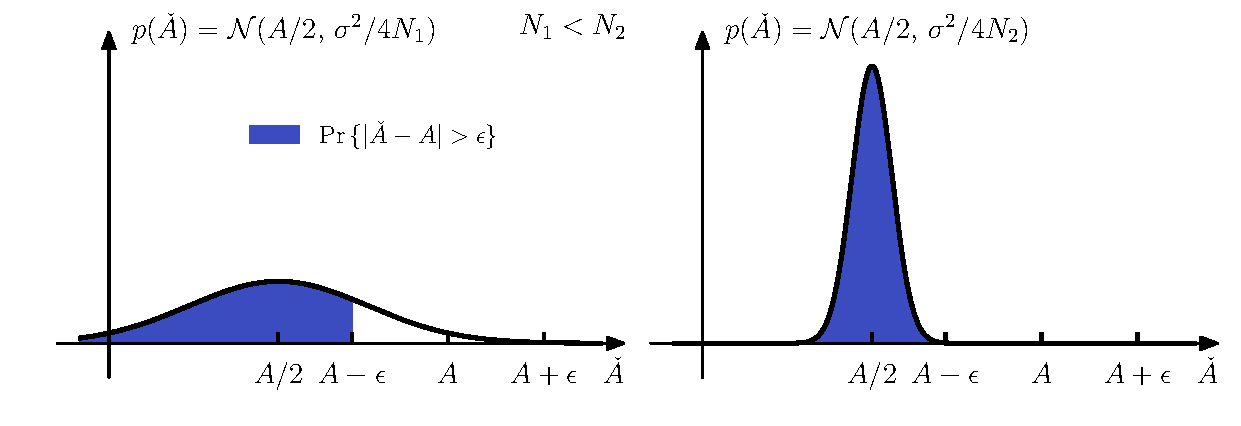
\includegraphics[width=0.92\textwidth]{figuras/problem_2_8.pdf}
\caption{\label{fig:problem_2_8} PDF de \(\check{A}\sim\mathcal{N}(A/2,\,\sigma^2/4N)\) para dos valores \(N_1\) y \(N_2\) de \(N\) con \(N_1<N_2\). El área sombreada es \(\Pr\big\{|\check{A}-A|>\epsilon\big\}\), que tiende a 1 cuando \(N\to\infty\) si \(\epsilon\in(0,\,A/2)\).}
\end{center}
\end{figure}

\subsection{Problema 9}

Este problema ilustra lo que ocurre con un estimador insesgado cuando se le aplica una transformación no lineal. En el problema de estimación de nivel de DC en WGN, se elige estimar el parámetro \(\theta=A^2\) como
\[
 \hat{\theta}=\left(\frac{1}{N}\sum_{n=0}^{N-1}x[n]\right)^2.
\]
¿Este estimador es insesgado? ¿Qué ocurre cuando \(N\to\infty\)?

\paragraph{Solución} Para verificar si el estimador es insesgado, hay que calcular su esperanza y ver si coincide con el valor verdadero del parámetro. Para hacerlo, se parte observando que
\begin{align*}
 \hat{\theta}&=\left(\frac{1}{N}\sum_{n=0}^{N-1}x[n]\right)^2\\
  &=\left(\frac{1}{N}\sum_{m=0}^{N-1}x[m]\right)\left(\frac{1}{N}\sum_{n=0}^{N-1}x[n]\right)\\
  &=\frac{1}{N^2}\sum_{m=0}^{N-1}\sum_{n=0}^{N-1}x[m]x[n]\\
  &=\frac{1}{N^2}\sum_{n=0}^{N-1}x^2[n]+\frac{1}{N^2}\sum_{m=0}^{N-1}\sum_{\substack{n=0 \\ n\neq m}}^{N-1}x[m]x[n],
\end{align*}
y por lo tanto,
\begin{align*}
 E(\hat{\theta})&=\frac{1}{N^2}\sum_{n=0}^{N-1}E(x^2[n])+\frac{1}{N^2}\sum_{m=0}^{N-1}\sum_{\substack{n=0 \\ n\neq m}}^{N-1}E(x[m]x[n])\\
 &\overset{(a)}{=}\frac{1}{N^2}\sum_{n=0}^{N-1}E(x^2[n])+\frac{1}{N^2}\sum_{m=0}^{N-1}\sum_{\substack{n=0 \\ n\neq m}}^{N-1}E(x[m])E(x[n])\\
 &\overset{(b)}{=}\frac{1}{N^2}\sum_{n=0}^{N-1}(A^2+\sigma^2)+\frac{1}{N^2}\sum_{m=0}^{N-1}\sum_{\substack{n=0 \\ n\neq m}}^{N-1}A^2\\
 &\overset{(c)}{=}\frac{1}{N^2}N(A^2+\sigma^2)+\frac{1}{N^2}N(N-1)A^2\\
 &=A^2+\frac{\sigma^2}{N},
\end{align*}
donde en \((a)\) se consideró que como el ruido \(w[n]\) es blanco, \(x[m]\) y \(x[n]\) son no correlacionadas si \(m\neq n\) y por lo tanto \(E(x[m]x[n])=E(x[m])E(x[n])\), en \((b)\) se tuvo en cuenta que
\[
 \var(x[n])=E(x^2[n])-E^2(x[n])\qquad\Rightarrow\qquad E(x^2[n])=E^2(x[n])+\var(x[n])=A^2+\sigma^2
\]
y en \((c)\) que la primer sumatoria tiene \(N\) sumandos y la segunda doble sumatoria tiene \(N(N-1)\) sumandos. Se concluye que
\[
 E(\hat{\theta})=A^2+\frac{\sigma^2}{N}\neq A^2,
\]
y por lo tanto \(\hat{\theta}\) no es un estimador insesgado. Sin embargo, se cumple que
\[
 \lim_{N\to\infty}E(\hat{\theta})=\lim_{N\to\infty}A^2+\frac{\sigma^2}{N}=A^2,
\]
es decir, \(\hat{\theta}\) es insesgado con \(N\to\infty\). Cuando esto ocurre, se dice que el estimador es \emph{asintóticamente insesgado}.

El cálculo de \(E(\hat{\theta})\) se puede realizar de forma mas directa considerando que \(\hat{\theta}=\hat{A}^2\), con \(\hat{A}\sim\mathcal{N}(A,\,\sigma^2/N)\), como se calculó en el problema de la sección \ref{sec:problem_2_3}. De esta forma
\[
 E(\hat{\theta})=E(\hat{A}^2)\qquad\textrm{y}\qquad \var(\hat{A})=E(\hat{A}^2)-E^2(\hat{A})\quad\Rightarrow\quad E(\hat{A}^2)=E^2(\hat{A})+\var(\hat{A})=A^2+\frac{\sigma^2}{N}.
\]

\subsection{Problema 10}

En el problema de estimación de nivel de DC en WGN, se asume ahora que además del parámetro \(A\) también se desconoce el parámetro \(\sigma^2\). Se desea estimar el parámetro vectorial
\[
 \bm{\theta}=
 \begin{bmatrix}
    A \\
    \sigma^2
 \end{bmatrix}.
\]
¿Es el estimador
\[
 \bm{\hat{\theta}}=
 \begin{bmatrix}
    \hat{A} \\
    \hat{\sigma^2}
 \end{bmatrix}=
\begin{bmatrix}
    \displaystyle\frac{1}{N}\sum_{n=0}^{N-1}x[n]\\
    \displaystyle\frac{1}{N-1}\sum_{n=0}^{N-1}\left(x[n]-\hat{A}\right)^2
 \end{bmatrix}
\]
insesgado?

\paragraph{Solución} Como ya se demostró en el problema de la sección \ref{sec:problema_1_4}, \(E(\hat{A})=A\), es decir, la media muestral \(\hat{A}\) es un estimador insesgado de \(A\). Falta ver si se cumple que \(E(\hat{\sigma^2})=\sigma^2\). Se comienza observando que
\begin{equation}\label{eq:problema_2_10_tmp1}
 E(\hat{\sigma^2})=\frac{1}{N-1}\sum_{n=0}^{N-1}E\left[\left(x[n]-\hat{A}\right)^2\right]
\end{equation}
La esperanza en la sumatoria se desarrolla como
\begin{equation}\label{eq:problema_2_10_tmp2}
 E\left[\left(x[n]-\hat{A}\right)^2\right]=E(x^2[n])-2E(x[n]\hat{A})+E(\hat{A}^2).
\end{equation}
Como \(x[n]\sim\mathcal{N}(A,\,\sigma^2)\), el primer sumando es
\[
 E(x^2[n])=\var(x[n])+E^2(x[n])=\sigma^2+A^2.
\]
Además, como \(\hat{A}\sim\mathcal{N}(A,\,\sigma^2/N)\) (ver el problema de la sección \ref{sec:problem_2_3}), el tercer sumando es
\[
 E(\hat{A}^2)=\var(\hat{A})+E^2(\hat{A})=\frac{\sigma^2}{N}+A^2.
\]
El segundo sumando puede calcularse como sigue:
\begin{align*}
 E(x[n]\hat{A})&=E\left(x[n]\frac{1}{N}\sum_{m=0}^{N-1}x[m]\right)\\
   &=\frac{1}{N}\sum_{m=0}^{N-1}E\left(x[n]x[m]\right)\\
   &=\frac{1}{N}\left[E(x^2[n])+\sum_{\substack{m=0 \\ m\neq n}}^{N-1}E(x[n])E(x[m])\right]\\
   &=\frac{1}{N}\left[\left(\sigma^2+A^2\right)+(N-1)A^2\right]\\
   &=\frac{\sigma^2}{N}+A^2.
\end{align*}
Sustituyendo estos resultados en la ecuación \ref{eq:problema_2_10_tmp2}, se tiene que
\[
 E\left[\left(x[n]-\hat{A}\right)^2\right]=(\sigma^2+A^2)-2\left(\frac{\sigma^2}{N}+A^2\right)+\left(\frac{\sigma^2}{N}+A^2\right)
 =\frac{N-1}{N}\sigma^2,
\]
y finalmente, sustituyendo este resultado en la ecuación \ref{eq:problema_2_10_tmp1} se llega a que
\[
 E(\hat{\sigma^2})=\frac{1}{N-1}\sum_{n=0}^{N-1}\frac{N-1}{N}\sigma^2=\sigma^2.
\]
Se concluye que \(E(\bm{\hat{\theta}})=\bm{\theta}\), es decir, el estimador vectorial es insesgado.

\subsection{Problema 11}

Dada un única observación \(x[0]\) de distribución \(\mathcal{U}[0,\,1/\theta]\), se quiere estimar \(\theta\). Se asume que \(\theta>0\). Mostrar que para que un estimador \(\hat{\theta}=g(x[0])\) sea insesgado, se tiene que cumplir que
\[
 \int_{0}^{1/\theta}g(u)du=1.
\]
Luego, mostrar que no existe una función \(g\) que cumpla esta condición para todo \(\theta>0\).

\paragraph{Solución} La PDF de la observación es
\[
 x[0]\sim p(x[0])=\mathcal{U}[0,\,1/\theta]=
 \left\{\begin{array}{ll}
  \theta, & 0 \leq x[0] \leq 1/\theta\\
  0, & \textrm{en otro caso}
 \end{array}, \right.
\]
y por lo tanto, la esperanza del estimador es
\[
 E(\hat{\theta})=E(g(x[0]))=\int_{-\infty}^{\infty}g(x[0])p(x[0])\,dx[0]
  =\int_{0}^{1/\theta}g(x[0])\theta\,dx[0]
  =\theta\int_{0}^{1/\theta}g(x[0])\,dx[0]
\]
Para que el estimador sea insesgado se tiene que cumplir que \(E(\hat{\theta})=\theta\), y por lo tanto
\[
 \theta\int_{0}^{1/\theta}g(x[0])\,dx[0]=\theta\qquad\Rightarrow\qquad \int_{0}^{1/\theta}g(u)\,du=1,
\]
que es lo se quería demostrar.

A continuación, se demostrará que no se puede encontrar una función \(g\) que cumpla esta condición para todo \(\theta\). Para hacerlo, se considera \(\theta_1\) y \(\theta_2\) tal que \(\theta_2<\theta_1\). De esta forma, hay que encontrar una función \(g\) tal que, 
\[
 \int_{0}^{1/\theta_1}g(u)\,du=1,\qquad\qquad \int_{0}^{1/\theta_2}g(u)\,du=1.
\]
Restando ambas ecuaciones, se tiene que
\[
 \int_{0}^{1/\theta_2}g(u)\,du-\int_{0}^{1/\theta_1}g(u)\,du=0\qquad\Rightarrow\qquad
 \int_{1/\theta_1}^{1/\theta_2}g(u)\,du=0\qquad\forall\;\theta_2<\theta_1.
\]
La única forma que se cumpla esta condición es que \(g(u)=0\) para todo \(u>0\), función que produce un estimador sesgado,
\[
 E(\hat{\theta})=E(g(x[0]))=E(0)=0\qquad \forall\;x[0],\quad\forall\;\theta>0.
\]

\chapter{Cota Inferior de Cramer-Rao}\label{ch:crlb}

\section{Cota Inferior de Cramer-Rao: parámetro escalar}

La cota inferior de Cramer-Rao (\emph{Cramer-Rao lower bond}, CRLB) es el valor mínimo que puede alcanzar la varianza de cualquier estimador.

\subsection{Teorema}\label{sec:crlb_scalar} 

\paragraph{Hipótesis} Sea el conjunto de datos \(\x\) con PDF \(p(\x;\,\theta)\), donde \(\theta\) es una constante determinística desconocida. Se asume que \(p(\x;\,\theta)\) satisface la siguiente \emph{condición de regularidad}:
\[
 E\left[\frac{\partial\ln p(\x;\,\theta)}{\partial\theta}\right]=0,\qquad\forall\,\theta,
\]
donde la esperanza se toma respecto a \(p(\x;\,\theta)\). 

\paragraph{Tesis} La varianza de cualquier estimador insesgado \(\hat{\theta}\) cumple que
\begin{equation}\label{eq:crlb_scalar}
 \var(\hat{\theta})\geq\frac{1}{I(\theta)},
\end{equation}
donde
\begin{equation}\label{eq:crlb_fisher_information}
 I(\theta)=-E\left[\dfrac{\partial^2\ln p(\x;\,\theta)}{\partial\theta^2}\right],
\end{equation}
función que es referida como la \emph{información de Fisher} de los datos \(\x\). En \(I(\theta)\), la derivada se evalúa en el valor verdadero de \(\theta\) y la esperanza se toma respecto a \(p(\x;\,\theta)\). 

Además, existe un estimador que alcanza la cota para todo \(\theta\) si y solo si
\begin{equation}\label{eq:crlb_efficiency_condition}
 \frac{\partial\ln p(\x;\,\theta)}{\partial\theta}=I(\theta)(g(\x)-\theta)
\end{equation}
para alguna función \(g\). Este estimador, que es el estimador \emph{insesgado de varianza mínima} (\emph{minimum variance unbiased} estimator, MVU), es \(\hat{\theta}=g(\x)\) y su varianza es \(1/I(\theta)\).

\paragraph{Demostración} Previo a la demostración, se examinará la condición de regularidad,
\[
 E\left[\frac{\partial\ln p(\x;\,\theta)}{\partial\theta}\right]=0,
\]
la cual se asume que se cumple. Observando que
\begin{align*}
 E\left[\frac{\partial\ln p(\x;\,\theta)}{\partial\theta}\right]&=\int\frac{\partial\ln p(\x;\,\theta)}{\partial\theta}p(\x;\,\theta)\,d\x\\
  &=\int\frac{1}{p(\x;\,\theta)}\frac{\partial p(\x;\,\theta)}{\partial\theta}p(\x;\,\theta)\,d\x\\
  &=\int\frac{\partial p(\x;\,\theta)}{\partial\theta}\,d\x\\
  &=\frac{\partial}{\partial\theta}\int p(\x;\,\theta)\,d\x\\
  &=\frac{\partial1}{\partial\theta}\\
  &=0,
\end{align*}
se concluye que la condición de regularidad se cumple siempre y cuando sea posible intercambiar el orden de integración y diferenciación. Esto en general puede hacerse  excepto cuando el soporte de la PDF depende del parámetro \(\theta\) (ver el problema de la sección \ref{sec:problem_3_1}).

Para la demostración del teorema, considérense las siguientes variables aleatorias:
\begin{equation}\label{eq:crlb_deduction_yz}
 y=\hat{\theta}(\x)-\theta,\qquad\qquad z=\frac{\partial\ln p(\x;\,\theta)}{\partial\theta},
\end{equation}
las cuales tienen media nula, \(y\) por ser \(\hat{\theta}\) insesgado y \(z\) porque se cumple la condición de regularidad. Se demostrará que \(E(yz)=1\),
\begin{align*}
 E(yz)&=E\left[(\hat{\theta}(\x)-\theta)\frac{\partial\ln p(\x;\,\theta)}{\partial\theta}\right]\\
  &=E\left[\hat{\theta}(\x)\frac{\partial\ln p(\x;\,\theta)}{\partial\theta}\right]-\theta E\left[\frac{\partial\ln p(\x;\,\theta)}{\partial\theta}\right]\\
  &\overset{(a)}{=}\int\hat{\theta}(\x)\frac{\partial\ln p(\x;\,\theta)}{\partial\theta}p(\x;\,\theta)\,d\x\\
  &=\int\hat{\theta}(\x)\frac{\partial p(\x;\,\theta)}{\partial\theta}\,d\x\\
  &\overset{(b)}{=}\frac{\partial}{\partial\theta}\int\hat{\theta}(\x) p(\x;\,\theta)\,d\x\\
  &=\frac{\partial}{\partial\theta}E[\hat{\theta}(\x)]\\
  &=\frac{\partial\theta}{\partial\theta}\\
  &=1,
\end{align*}
donde en \((a)\) se tuvo en cuenta que el segundo sumando es la condición de regularidad y por lo tanto es nulo y además se aplicó la definición de esperanza, y en \((b)\) se intercambió el orden de integración y diferenciación considerando que \(\hat{\theta}(\x)\) no depende de \(\theta\). Como \(E(yz)=1\), también se cumple que
\(E^2(yz)=1\), así que
\begin{align*}
 1&=E^2(yz)\\
    &\overset{(a)}{\leq}E(y^2)E(z^2)\\
    &=E\left[\left(\hat{\theta}(\x)-\theta\right)^2\right]E\left[\left(\frac{\partial\ln p(\x;\,\theta)}{\partial\theta}\right)^2\right]\\
    &\overset{(b)}{=}-E\left[\left(\hat{\theta}(\x)-\theta\right)^2\right]E\left[\frac{\partial^2\ln p(\x;\,\theta)}{\partial\theta^2}\right]\\
    &=\var(\hat{\theta})I(\theta),
\end{align*}
resultando en
\[
 \var(\hat{\theta})\geq\frac{1}{I(\theta)},
\]
que es la primera parte de la tesis.
En esta deducción, en \((a)\) se empleó el análogo de la desigualdad de Cauchy-Schwarz para variables aleatorias, que indica que si \(y\) y \(z\) son variables aleatorias,
\begin{equation}\label{eq:crlb_cauchy_schwarz_inequality}
 E^2(yz)\leq E(y^2)E(z^2).
\end{equation}
Para demostrarlo (ver el capítulo 6 de \cite{papoulis2002probability}) se observa que si \(c\) es una constante
\[
 E\left[(cy-z)^2\right]=E\left[c^2y^2-2cyz+z^2\right]=c^2E(y^2)-2cE(yz)+E(z^2)\geq0,\qquad\forall\,c,
\]
ya que la variable aleatoria \((cy-z)^2\) es no negativa y por lo tanto, su media también es no negativa. Por lo tanto, el discriminante del polinomio en \(c\) debe ser negativo o nulo,
\[
 \Delta=4E^2(zy)-4E(y^2)E(z^2)\leq0\qquad\Leftrightarrow\qquad E^2(zy)\leq E(y^2)E(z^2).
\]
Además, en \((b)\) se consideró que
\begin{equation}\label{eq:crlb_second_derivative_expectation}
 E\left[\left(\frac{\partial\ln p(\x;\,\theta)}{\partial\theta}\right)^2\right]=
 -E\left[\frac{\partial^2\ln p(\x;\,\theta)}{\partial\theta^2}\right].
\end{equation}
Esta igualdad proviene de la condición de regularidad. Efectivamente, la condición de regularidad indica que
\[
 \int\frac{\partial\ln p(\x;\,\theta)}{\partial\theta}p(\x;\,\theta)\,d\x=0,\qquad\forall\,\theta.
\]
Diferenciando respecto a \(\theta\) se observa que
\begin{align*}
 0&=\frac{\partial}{\partial\theta}\int\frac{\partial\ln p(\x;\,\theta)}{\partial\theta}p(\x;\,\theta)\,d\x\\
  &=\int\frac{\partial}{\partial\theta}\left[\frac{\partial\ln p(\x;\,\theta)}{\partial\theta}p(\x;\,\theta)\right]\,d\x\\
  &=\int\left[\frac{\partial^2\ln p(\x;\,\theta)}{\partial\theta^2}p(\x;\,\theta)+\frac{\partial\ln p(\x;\,\theta)}{\partial\theta}\frac{\partial p(\x;\,\theta)}{\partial\theta}\right]\,d\x\\
  &\overset{(a)}{=}\int\left[\frac{\partial^2\ln p(\x;\,\theta)}{\partial\theta^2}p(\x;\,\theta)+\frac{\partial\ln p(\x;\,\theta)}{\partial\theta}\frac{\partial\ln p(\x;\,\theta)}{\partial\theta}p(\x;\,\theta)\right]\,d\x,
\end{align*}
donde en \((a)\) se tomó en cuenta que
\begin{equation}\label{eq:crlb_logarithm_derivative}
 \frac{\partial\ln p(\x;\,\theta)}{\partial\theta}=\frac{1}{p(\x;\,\theta)}\frac{\partial p(\x;\,\theta)}{\partial\theta}
 \qquad\Rightarrow\qquad
 \frac{\partial p(\x;\,\theta)}{\partial\theta}=\frac{\partial\ln p(\x;\,\theta)}{\partial\theta}p(\x;\,\theta).
\end{equation}
Por lo tanto,
\[
 \int\left(\frac{\partial\ln p(\x;\,\theta)}{\partial\theta}\right)^2p(\x;\,\theta)\,d\x=
 -\int\frac{\partial^2\ln p(\x;\,\theta)}{\partial\theta^2}p(\x;\,\theta)\,d\x,
\]
que es la ecuación \ref{eq:crlb_second_derivative_expectation}.

Para demostrar la segunda parte de la tesis, se considera la condición de igualdad en la desigualdad de Cauchy-Schwarz (ecuación \ref{eq:crlb_cauchy_schwarz_inequality}). En la situación del teorema, las variables aleatorias \(y\) y \(z\), definidas en la ecuación \ref{eq:crlb_deduction_yz} son funciones de los datos \(\x\) y del parámetro \(\theta\). La condición de igualdad en la ecuación \ref{eq:crlb_cauchy_schwarz_inequality} es que \(cy=z\), donde \(c\) puede depender de \(\theta\) pero no de los datos \(\x\), ya que
\[
 E^2(yz)\overset{(a)}{=}E^2\left[c(\theta)y^2\right]=c^2(\theta)E^2\left(y^2\right)
\]
y
\[
 E(y^2)E(z^2)\overset{(a)}{=}E(y^2)E\left[c^2(\theta)y^2\right]=c^2(\theta)E^2\left(y^2\right),
\]
donde en \((a)\) se sustituyó \(z=c(\theta)y\), obteniendo que \(E^2(yz)=E(y^2)E(z^2)\). De esta forma, a partir de las definiciones de \(y\) y \(z\), la condición de igualdad es
\[
 \frac{\partial\ln p(\x;\,\theta)}{\partial\theta}=c(\theta)\left[\hat{\theta}(\x)-\theta\right].
\]
Para llegar a la ecuación \ref{eq:crlb_efficiency_condition}, hay que demostrar que \(c(\theta)=I(\theta)\). Esto puede hacerse derivando respecto a \(\theta\),
\[
 \frac{\partial^2\ln p(\x;\,\theta)}{\partial\theta^2}=\frac{\partial c(\theta)}{\partial \theta}\left[\hat{\theta}(\x)-\theta\right]-c(\theta),
\]
y tomando esperanza,
\[
 E\left[\frac{\partial^2\ln p(\x;\,\theta)}{\partial\theta^2}\right]=\frac{\partial c(\theta)}{\partial \theta}\left\{E\left[\hat{\theta}(\x)\right]-\theta\right\}-c(\theta)\overset{(a)}{=}-c(\theta),
\]
donde en \((a)\) se tuvo en cuenta que el estimador es insesgado. Como el lado izquierdo de la igualdad es \(-I(\theta)\) (ecuación \ref{eq:crlb_fisher_information}), se concluye que \(c(\theta)=I(\theta)\), finalizando la demostración.

En el caso en que la PDF de los datos está parametrizada por \(\theta\) y se desee encontrar un estimador insesgado \(\hat{\alpha}\) de \(\alpha=g(\theta)\), puede demostrarse de forma análoga que la CRLB está dada por
\begin{equation}\label{eq:crlb_parameter_transformation}
  \var(\hat{\alpha})=\frac{\left(\dfrac{\partial g(\theta)}{\partial\theta}\right)^2}{-E\left[\dfrac{\partial^2\ln p(\x;\,\theta)}{\partial\theta^2}\right]}.
\end{equation}

\subsubsection{Ejemplo: parámetros de ruido de Laplace}

Se consideran las observaciones \(\{x[0],\,x[1],\,\dots,\,x[N-1]\}\) IID con distribución de Laplace,
\[
 p(x;\,\mu,\,\sigma)=\frac{1}{\sqrt{2}\sigma}\exp\left(-\frac{\sqrt{2}|x-\mu|}{\sigma}\right).
\]
La PDF de las observaciones es
\begin{align*}
 p(\x;\,\mu,\,\sigma)&=\prod_{n=0}^{N-1}\frac{1}{\sqrt{2}\sigma}\exp\left(-\frac{\sqrt{2}|x[n]-\mu|}{\sigma}\right)\\
 &=\frac{1}{(\sqrt{2}\sigma)^N}\exp\left(-\frac{\sqrt{2}}{\sigma}\sum_{n=0}^{N-1}|x[n]-\mu|\right),
\end{align*}
por lo que la función de verosimilitud logarítmica es
\[
 \ln p(\x;\,\mu,\,\sigma)=-N\ln\sqrt{2}-N\ln\sigma-\frac{\sqrt{2}}{\sigma}\sum_{n=0}^{N-1}|x[n]-\mu|.
\]
Supóngase que la media \(\mu\) es conocida y se quiere encontrar el estimador MVU de la desviación estándar \(\sigma\). La derivada respecto al parámetro es
\[
 \frac{\partial\ln p(\x;\,\sigma)}{\partial\sigma}=-\frac{N}{\sigma}+\frac{\sqrt{2}}{\sigma^2}\sum_{n=0}^{N-1}|x[n]-\mu|,
\]
y observando que se puede factorizar de la forma de la ecuación \ref{eq:crlb_efficiency_condition} como
\[
 \frac{\partial\ln p(\x;\,\sigma)}{\partial\sigma}=\frac{N}{\sigma^2}\left(\frac{\sqrt{2}}{N}\sum_{n=0}^{N-1}|x[n]-\mu|-\sigma\right),
\]
se concluye que el estimador MVU es
\[
 \hat{\sigma}=\frac{\sqrt{2}}{N}\sum_{n=0}^{N-1}|x[n]-\mu|
\]
y la CRLB es
\[
 \var(\hat{\sigma})\geq\frac{\sigma^2}{N}.
\]
En este caso, como se cumple la condición de la ecuación \ref{eq:crlb_efficiency_condition}, el estimador es eficiente, es decir, alcanza la CRLB para todo valor del parámetro \(\sigma\).

Supóngase ahora que la desviación estándar \(\sigma\) es conocida y se quiere estimar la media \(\mu\). La derivada de la función de verosimilitud logarítmica es
\begin{align*}
 \frac{\partial\ln p(\x;\,\mu)}{\partial\mu}&=-\frac{\sqrt{2}}{\sigma}\sum_{n=0}^{N-1}\frac{\partial|x[n]-\mu|}{\partial\mu}\\
   &=\frac{\sqrt{2}}{\sigma}\sum_{n=0}^{N-1}\operatorname{sig}(x[n]-\mu),
\end{align*}
donde se tuvo en cuenta que \(\partial|x[n]-\mu|/\partial\mu=-\operatorname{sig}(x[n]-\mu)\).
Esta función no parece poder factorizarse en la forma de la ecuación \ref{eq:crlb_efficiency_condition}, y por lo tanto, mediante esta técnica no puede encontrarse un estimador MVU. Para determinar la CRLB, se deriva nuevamente,
\begin{align*}
 \frac{\partial^2\ln p(\x;\,\mu)}{\partial\mu^2}&=\frac{\sqrt{2}}{\sigma}\sum_{n=0}^{N-1}\frac{\partial\operatorname{sig}(x[n]-\mu)}{\partial\mu}\\
   &=-\frac{2\sqrt{2}}{\sigma}\sum_{n=0}^{N-1}\delta(x[n]-\mu),
\end{align*}
donde se tuvo en cuenta que \(\partial\operatorname{sig}(x[n]-\mu)/\partial\mu=-2\delta(x[n]-\mu)\).
Tomando esperanza, se tiene que la información de Fisher es
\begin{align*}
 I(\mu)=-E\left[\frac{\partial^2\ln p(\x;\,\mu)}{\partial\mu^2}\right]&=\frac{2\sqrt{2}}{\sigma}\sum_{n=0}^{N-1}E[\delta(x[n]-\mu)]\\
  &\overset{(a)}{=}\frac{2\sqrt{2}}{\sigma}\left(N\frac{1}{\sqrt{2}\sigma}\right)\\
  &=\frac{2N}{\sigma^2}
\end{align*}
donde en \((a)\) se consideró que
\begin{align*}
 E[\delta(x[n]-\mu)]&=\int_{-\infty}^{\infty}\delta(x[n]-\mu)\frac{1}{\sqrt{2}\sigma}\exp\left(-\frac{\sqrt{2}|x[n]-\mu|}{\sigma}\right)\,dx[n]\\
 &=\frac{1}{\sqrt{2}\sigma}\exp\left(-\frac{\sqrt{2}|x[n]-\mu|}{\sigma}\right)\bigg|_{x[n]=\mu}\\
 &=\frac{1}{\sqrt{2}\sigma}.
\end{align*}
Se concluye que la CLRB es
\[
 \var(\hat{\mu})\geq\frac{1}{I(\mu)}=\frac{\sigma^2}{2N}.
\]
Ver además el problema de la sección \ref{sec:problem_3_2}.

\subsection{Transformación de parámetros}

En frecuencia ocurre en la práctica que el parámetro que se quiere estimar es función de otro parámetro fundamental. Si se desea estimar \(\alpha=g(\theta)\), la CRLB es
\[
 \var(\hat{\alpha})\geq\dfrac{\left(\dfrac{\partial g}{\partial\theta}\right)^2}{-E\left[\dfrac{\partial^2\ln p(\x;\,\theta)}{\partial\theta^2}\right]}
\]
\paragraph{Demostración} Se demostrará que
\begin{equation}\label{eq:crlb_parameter_transformation_fisher}
 I^{-1}(\alpha)=I^{-1}(\theta)\left(\frac{\partial g}{\partial\theta}\right)^2,
\end{equation}
y por lo tanto, se cumple que
\[
\var(\alpha)\geq\frac{1}{I(\alpha)}=\dfrac{\left(\dfrac{\partial g}{\partial\theta}\right)^2}{I(\theta)}.
\]
Para mostrarlo, empleando la regla de la cadena, se cumple que
\[
 \frac{\partial\ln p(\x;\,\theta)}{\partial\theta}=\frac{\partial\ln p(\x;\,\theta)}{\partial\alpha}\frac{\partial\alpha}{\partial\theta}
\]
y derivando nuevamente,
\begin{align*}
 \frac{\partial^2\ln p(\x;\,\theta)}{\partial\theta^2}&=\frac{\partial}{\partial\theta}\left[\frac{\partial\ln p(\x;\,\theta)}{\partial\alpha}\right]\frac{\partial\alpha}{\partial\theta}+\frac{\partial\ln p(\x;\,\theta)}{\partial\alpha}\frac{\partial}{\partial\theta}\left[\frac{\partial\alpha}{\partial\theta}\right]\\
  &\overset{(a)}{=}\frac{\partial}{\partial\alpha}\left[\frac{\partial\ln p(\x;\,\theta)}{\partial\alpha}\right]\frac{\partial\alpha}{\partial\theta}\frac{\partial\alpha}{\partial\theta}+\frac{\partial\ln p(\x;\,\theta)}{\partial\alpha}\frac{\partial^2\alpha}{\partial\theta^2}\\
  &=\frac{\partial^2\ln p(\x;\,\theta)}{\partial\alpha^2}\left(\frac{\partial\alpha}{\partial\theta}\right)^2+\frac{\partial\ln p(\x;\,\theta)}{\partial\alpha}\frac{\partial^2\alpha}{\partial\theta^2},
\end{align*}
donde en \((a)\) se aplicó nuevamente la regla de la cadena en la derivada del primer sumando. Tomando esperanza en ambos lados de la igualdad, se tiene que
\[
 E\left[\frac{\partial^2\ln p(\x;\,\theta)}{\partial\theta^2}\right]=E\left[\frac{\partial^2\ln p(\x;\,\theta)}{\partial\alpha^2}\right]\left(\frac{\partial\alpha}{\partial\theta}\right)^2,
\]
resultando en que
\[
 I(\theta)=I(\alpha)\left(\frac{\partial g}{\partial\theta}\right)^2,
\]
que es lo que se quería demostrar.

\section{Cota Inferior de Cramer-Rao: parámetro vectorial}

En esta sección se deriva la CRLB para el caso de un parámetro vectorial \(\thetabf\), es decir, la PDF de los datos \(\x\) está caracterizada por un vector \(\thetabf\).

\subsection{Teorema} 

\paragraph{Hipótesis} Sea el conjunto de datos \(\x\) con PDF \(p(\x;\,\thetabf)\), donde \(\thetabf\) es un vector \(p\times1\) constante desconocido. Se asume que \(p(\x;\,\thetabf)\) satisface las \emph{condiciones de regularidad}
\[
 E\left[\frac{\partial\ln p(\x;\,\thetabf)}{\partial\thetabf}\right]=\bm{0},\qquad\forall\,\thetabf,
\]
donde la esperanza se toma respecto a \(p(\x;\,\thetabf)\). 

\paragraph{Tesis} La matriz de covarianza de cualquier estimador insesgado \(\hat{\thetabf}\) cumple que
\begin{equation}\label{eq:crlb_vector}
 \C_{\hat{\thetabf}}-\I^{-1}(\thetabf)\geq\bm{0},
\end{equation}
donde \(\geq\bm{0}\) se interpreta como que la matriz es semidefinida positiva. La \emph{matriz de información de Fisher} \(\I(\thetabf)\) esta dada por
\begin{equation}\label{eq:crlb_fisher_information_matrix}
 [\I(\thetabf)]_{ij}=-E\left[\dfrac{\partial^2\ln p(\x;\,\thetabf)}{\partial\theta_i\theta_j}\right],\qquad i=1,\dots,\,p,\quad j=1,\dots,\,p,
\end{equation}
donde las derivadas se evalúan en el valor verdadero de \(\thetabf\) y la esperanza se toma respecto a \(p(\x;\,\thetabf)\). 

Además, existe un estimador insesgado que alcanza la cota, en el sentido de que \(\C_{\hat{\thetabf}}=\I^{-1}(\thetabf)\) para todo \(\thetabf\) si y solo si
\begin{equation}\label{eq:crlb_efficiency_condition_vector}
 \frac{\partial\ln p(\x;\,\thetabf)}{\partial\thetabf}=\I(\thetabf)(\g(\x)-\thetabf)
\end{equation}
para alguna función \(\g\subset\mathbb{R}^p\) y alguna matriz \(\I\) \(p\times p\). Este estimador, que es el estimador MVU, es \(\hat{\thetabf}=\g(\x)\) y su matriz de covarianza es \(\I^{-1}(\thetabf)\).

Como los elementos de la diagonal de una matriz semidefinida positiva son no negativos, se cumple que
\[
 [\C_{\hat{\thetabf}}-\I^{-1}(\thetabf)]_{ii}\geq 0,
\]
y por lo tanto,
\begin{equation}\label{eq:crlb_vector_variance}
 \var(\hat{\thetabf}_i)=[\C_{\hat{\thetabf}}]_{ii}\geq[\I^{-1}(\thetabf)]_{ii}.
\end{equation}

\paragraph{Demostración} Se considerará el caso mas general en que el parámetro a estimar es una función \(\alphabf=\g(\thetabf)\) del parámetro vectorial \(\thetabf\)\footnote{No debe confundirse esta función \(\g\), que es una transformación del parámetro \(\thetabf\), con la función \(\g\) de la ecuación \ref{eq:crlb_efficiency_condition_vector}, que es el estimador MVU. Si bien la notación puede ser confusa, se pretende seguir lo mas fielmente posible la empleada en \cite{kay93fundamentals}}. La PDF de los datos \(\x\) está caracterizada por \(\thetabf\). El parámetro \(\thetabf\) tiene dimensiones \(p\times1\), \(\alphabf\) tiene dimensiones \(r\times1\) y \(\g:\mathbb{R}^p\to\mathbb{R}^r\). Se tendrán en cuenta los estimadores insesgados,
\[
 E(\hat{\alpha}_i)=\alpha_i=[\g(\thetabf)]_i,\qquad i=1,\dots,\,r.
\]

Se comienza notando que se cumple que
\[
 \int(\hat{\alpha}_i-\alpha_i)\frac{\partial\ln p(\x,\,\thetabf)}{\partial\theta_i}p(\x,\,\thetabf)\,d\x=\frac{\partial[\g(\thetabf)]_i}{\partial\theta_i}.
\]
Esto es consecuencia de las condiciones de regularidad, ya que
\begin{align*}
 \int(\hat{\alpha}_i-\alpha_i)\frac{\partial\ln p(\x,\,\thetabf)}{\partial\theta_i}p(\x,\,\thetabf)\,d\x&=\int \hat{\alpha}_i\frac{\partial\ln p(\x,\,\thetabf)}{\partial\theta_i}p(\x,\,\thetabf)\,d\x-\int\alpha_i\frac{\partial\ln p(\x,\,\thetabf)}{\partial\theta_i}p(\x,\,\thetabf)\,d\x\\
  &\overset{(a)}{=}\int \hat{\alpha}_i\frac{\partial p(\x,\,\thetabf)}{\partial\theta_i}\,d\x-\alpha_i\int\frac{\partial\ln p(\x,\,\thetabf)}{\partial\theta_i}p(\x,\,\thetabf)\,d\x\\
  &\overset{(b)}{=}\frac{\partial}{\partial\theta_i}\int\hat{\alpha}_ip(\x,\,\thetabf)\,d\x-\alpha_iE\left[\frac{\partial\ln p(\x;\,\thetabf)}{\partial\theta_i}\right]\\
  &\overset{(c)}{=}\frac{\partial E(\hat{\alpha}_i)}{\partial\theta_i}-0\\
  &=\frac{\partial [\g(\thetabf)]_i}{\partial\theta_i},
\end{align*}
donde en \((a)\) se aplicó la igualdad equivalente de la ecuación \ref{eq:crlb_logarithm_derivative} del caso escalar y además se consideró que \(\alpha_i\) es una constante por lo que puede sacarse de la integral, en \((b)\) se intercambió el orden de integración y diferenciación teniendo en cuenta que \(\hat{\alpha}_i\) depende de los datos \(\x\) pero no de \(\theta_i\) y en \((c)\) se consideró que el segundo sumando es la condición de regularidad y por lo tanto, es nulo. Realizando un razonamiento análogo para \(j\neq i\), puede verse que
\[
 \int(\hat{\alpha}_i-\alpha_i)\frac{\partial\ln p(\x,\,\thetabf)}{\partial\theta_j}p(\x,\,\thetabf)\,d\x=\frac{\partial[\g(\thetabf)]_i}{\partial\theta_j}.
\]
Combinando estos dos resultados en notación matricial, se llega a que
\[
 \int(\hat{\alphabf}-\alphabf)\frac{\partial\ln p(\x,\,\thetabf)}{\partial\thetabf}^Tp(\x,\,\thetabf)\,d\x=\frac{\partial\g(\thetabf)}{\partial\thetabf},
\]
donde
\[
\hat{\alphabf}-\alphabf=
 \begin{bmatrix}
  \hat{\alpha}_1-\alpha_1\\
  \vdots\\
  \hat{\alpha}_1-\alpha_r
 \end{bmatrix}
\qquad
\frac{\partial\ln p(\x,\,\thetabf)}{\partial\thetabf}=
 \begin{bmatrix}
  \dfrac{\partial\ln p(\x,\,\thetabf)}{\partial\theta_1}\\
  \vdots\\
  \dfrac{\partial\ln p(\x,\,\thetabf)}{\partial\theta_p}
 \end{bmatrix}
\qquad
 \frac{\partial\g(\thetabf)}{\partial\thetabf}=
 \begin{bmatrix}
    \dfrac{\partial g_1(\thetabf)}{\partial\theta_1} & \dfrac{\partial g_1(\thetabf)}{\partial\theta_2} & \dots & \dfrac{\partial g_1(\thetabf)}{\partial\theta_p}  \\
    \vdots & \vdots & & \vdots \\
    \dfrac{\partial g_r(\thetabf)}{\partial\theta_1} & \dfrac{\partial g_r(\thetabf)}{\partial\theta_2} & \dots & \dfrac{\partial g_r(\thetabf)}{\partial\theta_p}  \\
 \end{bmatrix}.
\]
Premultiplicando por \(\abf^T\) y postmultiplicando \(\bbf\) ambos lados de la igualdad, donde \(\abf\) y \(\bbf\) son vectores arbitrarios de dimensiones \(r\times1\) y \(p\times1\) respectivamente, se obtiene que
\begin{equation}\label{eq:crlb_vector_tmp1}
 \int\abf^T(\hat{\alphabf}-\alphabf)\frac{\partial\ln p(\x,\,\thetabf)}{\partial\thetabf}^T\bbf p(\x,\,\thetabf)\,d\x=\abf^T\frac{\partial\g(\thetabf)}{\partial\thetabf}\bbf,
\end{equation}
donde ahora la ecuación es escalar. Definiendo las variables aleatorias escalares
\begin{equation}\label{eq:crlb_vector_tmp3}
 y(\x)=\abf^T(\hat{\alphabf}-\alphabf),
 \qquad
 z(\x)=\frac{\partial\ln p(\x,\,\thetabf)}{\partial\thetabf}^T\bbf
\end{equation}
se tiene que
\begin{gather*}
 y(\x)z(\x)=\abf^T(\hat{\alphabf}-\alphabf)\frac{\partial\ln p(\x,\,\thetabf)}{\partial\thetabf}^T\bbf \\
 y(\x)y^T(\x)=y^2(\x)=\abf^T(\hat{\alphabf}-\alphabf)(\hat{\alphabf}-\alphabf)^T\abf\\
 z^T(\x)z(\x)=z^2(\x)=\bbf^T\frac{\partial\ln p(\x,\,\thetabf)}{\partial\thetabf}\frac{\partial\ln p(\x,\,\thetabf)}{\partial\thetabf}^T\bbf,
\end{gather*}
donde se consideró que \(y(\x)=y^T(\x)\) y \(z(\x)=z^T(\x)\) por ser escalares. Tomando la esperanza se obtiene que
\begin{equation}
 \begin{gathered}\label{eq:crlb_vector_tmp2}
 E[y(\x)z(\x)]=\int\abf^T(\hat{\alphabf}-\alphabf)\frac{\partial\ln p(\x,\,\thetabf)}{\partial\thetabf}^T\bbf\,p(\x,\,\thetabf)\,d\x\overset{(a)}{=}\abf^T\frac{\partial\g(\thetabf)}{\partial\thetabf}\bbf\\
 E[y^2(\x)]=E[\abf^T(\hat{\alphabf}-\alphabf)(\hat{\alphabf}-\alphabf)^T\abf]=\abf^TE[(\hat{\alphabf}-\alphabf)(\hat{\alphabf}-\alphabf)^T]\abf\overset{(b)}{=}\abf^T\C_{\hat{\alphabf}}\abf\\
 E[z^2(\x)]=E\left[\bbf^T\frac{\partial\ln p(\x,\,\thetabf)}{\partial\thetabf}\frac{\partial\ln p(\x,\,\thetabf)}{\partial\thetabf}^T\bbf\right]
 =\bbf^TE\left[\frac{\partial\ln p(\x,\,\thetabf)}{\partial\thetabf}\frac{\partial\ln p(\x,\,\thetabf)}{\partial\thetabf}^T\right]\bbf
 \overset{(c)}{=}\bbf^T\I(\thetabf)\bbf,
\end{gathered}
\end{equation}
donde la igualdad en \((a)\) proviene de la ecuación \ref{eq:crlb_vector_tmp1}, en \((b)\) se consideró que como \(E(\hat{\alphabf})=\alphabf\), \(\C_{\hat{\alphabf}}=E[(\hat{\alphabf}-\alphabf)(\hat{\alphabf}-\alphabf)^T]\) es la matriz de covarianza de \(\hat{\alphabf}\) y en \((c)\) se consideró que como en el caso escalar, se cumple que
\begin{equation}\label{eq:crlb_fisher_information_matrix_alt}
 E\left[\frac{\partial\ln p(\x,\,\thetabf)}{\partial\theta_i}\frac{\partial\ln p(\x,\,\thetabf)}{\partial\theta_j}\right]=
 -E\left[\frac{\partial^2\ln p(\x,\,\thetabf)}{\partial\theta_i\partial\theta_j}\right]
 =[\I(\thetabf)]_{ij}, 
\end{equation}
donde \(\I(\thetabf)\) es la matriz de información de Fisher. Esta igualdad proviene de la condición de regularidad,
\[
 \int\frac{\partial\ln p(\x,\,\thetabf)}{\partial\theta_i}p(\x,\,\thetabf)\,d\x=0,
\]
ya que diferenciando ambos lados de la igualdad respecto a \(\theta_j\), se observa que
\begin{align*}
 0&=\frac{\partial}{\partial\theta_j}\int\frac{\partial\ln p(\x,\,\thetabf)}{\partial\theta_i}p(\x,\,\thetabf)\,d\x\\
  &=\int\frac{\partial}{\partial\theta_j}\left[\frac{\partial\ln p(\x,\,\thetabf)}{\partial\theta_i}p(\x,\,\thetabf)\right]\,d\x\\
  &=\int\left[\frac{\partial^2\ln p(\x,\,\thetabf)}{\partial\theta_i\theta_j}p(\x,\,\thetabf)+\frac{\partial\ln p(\x,\,\thetabf)}{\partial\theta_i}\frac{\partial p(\x,\,\thetabf)}{\partial\theta_j}\right]\,d\x\\
  &=\int\frac{\partial^2\ln p(\x,\,\thetabf)}{\partial\theta_i\theta_j}p(\x,\,\thetabf)\,d\x+\int\frac{\partial\ln p(\x,\,\thetabf)}{\partial\theta_i}\frac{\partial\ln p(\x,\,\thetabf)}{\partial\theta_j}p(\x,\,\thetabf)\,d\x\\
  &=E\left[\frac{\partial^2\ln p(\x,\,\thetabf)}{\partial\theta_i\partial\theta_j}\right]+E\left[\frac{\partial\ln p(\x,\,\thetabf)}{\partial\theta_i}\frac{\partial\ln p(\x,\,\thetabf)}{\partial\theta_j}\right].
\end{align*}
Finalmente, aplicando la desigualdad de Cauchy-Schwarz \(E^2(yz)\leq E(y^2)E(z^2)\) (ecuación \ref{eq:crlb_cauchy_schwarz_inequality}) en las ecuaciones \ref{eq:crlb_vector_tmp2} se llega a que
\[
 \left(\abf^T\frac{\partial\g(\thetabf)}{\partial\thetabf}\bbf\right)^2
 \leq\abf^T\C_{\hat{\alphabf}}\abf\bbf^T\I(\thetabf)\bbf.
\]
Teniendo en cuenta que \(\bbf\) es arbitrario, definase como
\begin{equation}\label{eq:crlb_vector_tmp4}
 \bbf=\I^{-1}(\thetabf)\frac{\partial\g(\thetabf)}{\partial\thetabf}^T\abf.
\end{equation}
De esta forma,
\[
 \left(\abf^T\frac{\partial\g(\thetabf)}{\partial\thetabf}\I^{-1}(\thetabf)\frac{\partial\g(\thetabf)}{\partial\thetabf}^T\abf\right)^2
 \leq
 \abf^T\C_{\hat{\alphabf}}\abf\left(\abf^T\frac{\partial\g(\thetabf)}{\partial\thetabf}[\I^{-1}(\thetabf)]^T\I(\thetabf)\I^{-1}(\thetabf)\frac{\partial\g(\thetabf)}{\partial\thetabf}^T\abf\right).
\]
Considerando que la matriz \(\I(\thetabf)\) es simétrica y definida positiva, ya que
\[
 \ubf^TE[\vbf\vbf^T]\ubf=E[\ubf^T\vbf\vbf^T\ubf]=E[(\ubf^T\vbf)(\ubf^T\vbf)^T]=E[(\ubf^T\vbf)^2]>0,\qquad\forall\ubf>\bm{0},
\]
también lo es \(\I^{-1}(\thetabf)\), y por lo tanto \([\I^{-1}(\thetabf)]^T=\I^{-1}(\thetabf)\), por lo que
\[
 \left(\abf^T\frac{\partial\g(\thetabf)}{\partial\thetabf}\I^{-1}(\thetabf)\frac{\partial\g(\thetabf)}{\partial\thetabf}^T\abf\right)^2
 \leq
 \abf^T\C_{\hat{\alphabf}}\abf\left(\abf^T\frac{\partial\g(\thetabf)}{\partial\thetabf}\I^{-1}(\thetabf)\frac{\partial\g(\thetabf)}{\partial\thetabf}^T\abf\right)
\]
y cancelando el término entre paréntesis, se tiene que
\[
 \abf^T\frac{\partial\g(\thetabf)}{\partial\thetabf}\I^{-1}(\thetabf)\frac{\partial\g(\thetabf)}{\partial\thetabf}^T\abf
 \leq
 \abf^T\C_{\hat{\alphabf}}\abf,
\]
por lo que
\[
 \abf^T\C_{\hat{\alphabf}}\abf-\abf^T\frac{\partial\g(\thetabf)}{\partial\thetabf}\I^{-1}(\thetabf)\frac{\partial\g(\thetabf)}{\partial\thetabf}^T\abf\geq0,
\]
resultando en
\[
 \abf^T\left(\C_{\hat{\alphabf}}-\frac{\partial\g(\thetabf)}{\partial\thetabf}\I^{-1}(\thetabf)\frac{\partial\g(\thetabf)}{\partial\thetabf}^T\right)\abf\geq0.
\]
Como \(\abf\) es arbitrario, la desigualdad se cumple para todo \(\abf\). Se concluye que la matriz entre paréntesis es semidefinida positiva, 
\begin{equation}\label{eq:crlb_vector_transformations}
 \C_{\hat{\alphabf}}-\frac{\partial\g(\thetabf)}{\partial\thetabf}\I^{-1}(\thetabf)\frac{\partial\g(\thetabf)}{\partial\thetabf}^T\geq\bm{0}.
\end{equation}
En el caso en que no haya una transformación del parámetro, \(\alphabf=\g(\thetabf)=\thetabf\) y \(\frac{\partial\g(\thetabf)}{\partial\thetabf}=\I\) obteniéndose la ecuación
\ref{eq:crlb_vector}, con lo que queda demostrada la primera parte del teorema.

Como se mostró en la sección \ref{sec:crlb_scalar}, la condición de igualdad en la ecuación de Cauchy-Schwarz es que \(y(\x)=c(\thetabf)z(\x)\), donde \(c(\thetabf)\) es una constante que puede depender de \(\thetabf\) pero no de los datos \(\x\). A partir de las definiciones de \(y(\x)\) y \(z(\x)\) (ecuación \ref{eq:crlb_vector_tmp3}), la condición es
\begin{align*}
 \abf^T(\hat{\alphabf}-\alphabf)&=c(\thetabf)\frac{\partial\ln p(\x,\,\thetabf)}{\partial\thetabf}^T\bbf\\
  &\overset{(a)}{=}c(\thetabf)\frac{\partial\ln p(\x,\,\thetabf)}{\partial\thetabf}^T\I^{-1}(\thetabf)\frac{\partial\g(\thetabf)}{\partial\thetabf}^T\abf
\end{align*}
donde en \((a)\) se sustituyó \(\bbf\) a partir de la ecuación \ref{eq:crlb_vector_tmp4}.
Esta ecuación es escalar de la forma \(\abf^T\ubf=\vbf^T\abf\), por lo que la única forma de que se cumpla para todo \(\abf\), ya que \(\abf\) es arbitrario, es que \(\ubf=\vbf\), y por lo tanto,
\[
 \hat{\alphabf}-\alphabf=c(\thetabf)\frac{\partial\g(\thetabf)}{\partial\thetabf}\I^{-1}(\thetabf)\frac{\partial\ln p(\x,\,\thetabf)}{\partial\thetabf}.
\]
En el caso en que \(\alphabf=\g(\thetabf)=\thetabf\) y \(\frac{\partial\g(\thetabf)}{\partial\thetabf}=\I\) se tiene que
\[
 \hat{\thetabf}-\thetabf=c(\thetabf)\I^{-1}(\thetabf)\frac{\partial\ln p(\x,\,\thetabf)}{\partial\thetabf},
\]
y por lo tanto, despejando, se obtiene que
\[
 \frac{\partial\ln p(\x,\,\thetabf)}{\partial\thetabf}=\frac{1}{c(\thetabf)}\I(\thetabf)(\hat{\thetabf}-\thetabf).
\]
Para finalizar la prueba, se demostrará que \(c(\thetabf)=1\) para obtener la ecuación \(\ref{eq:crlb_efficiency_condition_vector}\).
El elemento \(i\)-ésimo de este vector es
\[
 \frac{\partial\ln p(\x,\,\thetabf)}{\partial\theta_i}=\sum_{k=1}^{p}\frac{[\I(\thetabf)]_{ik}}{c(\thetabf)}(\hat{\theta}_k-\theta_k).
\]
Diferenciando una vez mas, se ve que
\begin{align*}
 \frac{\partial^2\ln p(\x,\,\thetabf)}{\partial\theta_i\partial\theta_j}&=\frac{\partial}{\partial\theta_j}\left(\sum_{k=1}^{p}\frac{[\I(\thetabf)]_{ik}}{c(\thetabf)}(\hat{\theta}_k-\theta_k)\right)\\
  &=\sum_{k=1}^{p}\frac{[\I(\thetabf)]_{ik}}{c(\thetabf)}\frac{\partial(\hat{\theta}_k-\theta_k)}{\partial\theta_j}+\sum_{k=1}^{p}\frac{\partial\left(\dfrac{[\I(\thetabf)]_{ik}}{c(\thetabf)}\right)}{\partial\theta_j}(\hat{\theta}_k-\theta_k)\\
  &\overset{(a)}{=}-\frac{[\I(\thetabf)]_{ij}}{c(\thetabf)}+\sum_{k=1}^{p}\frac{\partial\left(\dfrac{[\I(\thetabf)]_{ik}}{c(\thetabf)}\right)}{\partial\theta_j}(\hat{\theta}_k-\theta_k),
\end{align*}
donde en \((a)\) se tuvo en cuenta que \(\partial(\hat{\theta}_k-\theta_k)/\partial\theta_j\) es 0 si \(k\neq j\) y \(-1\) si \(k=j\). Tomando la esperanza, se tiene que
\begin{align*}
 E\left[\frac{\partial^2\ln p(\x,\,\thetabf)}{\partial\theta_i\partial\theta_j}\right]
  &=E\left[-\frac{[\I(\thetabf)]_{ij}}{c(\thetabf)}+\sum_{k=1}^{p}\frac{\partial\left(\dfrac{[\I(\thetabf)]_{ik}}{c(\thetabf)}\right)}{\partial\theta_j}(\hat{\theta}_k-\theta_k)\right]\\
  &=-\frac{[\I(\thetabf)]_{ij}}{c(\thetabf)}+\sum_{k=1}^{p}\frac{\partial\left(\dfrac{[\I(\thetabf)]_{ik}}{c(\thetabf)}\right)}{\partial\theta_j}\left[E(\hat{\theta}_k)-\theta_k\right]\\
  &=-\frac{[\I(\thetabf)]_{ij}}{c(\thetabf)},
\end{align*}
ya que \(E(\hat{\theta}_k)=\theta_k\). Como el lado izquierdo de la igualdad es \(-[\I(\thetabf)]_{ij}\), se concluye que \(c(\thetabf)=1\). 

\subsection{Ejemplo: nivel de DC en WGN}\label{sec:crlb_dc_in_wgn_dc_and_variance}

Se considera el problema de estimación del nivel de DC en WGN. El modelo de los datos es
\[
 x[n]=A+w[n],\qquad n=0,\dots,\,N-1,
\]
donde los parámetros a estimar son el nivel \(A\) de DC y la varianza \(\sigma^2\) del ruido \(w[n]\sim\mathcal{N}(0,\,\sigma^2)\). El parámetro vectorial es \(\thetabf=[A\,\sigma^2]^T\) y por lo tanto, \(p=2\). La matriz \(2\times2\) de información de Fisher es
\begin{equation*}
 \renewcommand*{\arraystretch}{2.8}
 I(\thetabf)=
 \begin{bmatrix}
    -E\left[\dfrac{\partial^2\ln p(\x,\,\thetabf)}{\partial A^2}\right] & -E\left[\dfrac{\partial^2\ln p(\x,\,\thetabf)}{\partial A\partial\sigma^2}\right]\\
     -E\left[\dfrac{\partial^2\ln p(\x,\,\thetabf)}{\partial\sigma^2\partial A}\right] & 
     -E\left[\dfrac{\partial^2\ln p(\x,\,\thetabf)}{\partial {\sigma^2}^2}\right]
 \end{bmatrix}.
\end{equation*}
La matriz de información de Fisher es simétrica y puede demostrarse que es definida positiva, como se hace en el problema \ref{sec:problem_3_10}. La PDF de los datos es
\[
 p(\x;\,\thetabf)=\frac{1}{(2\pi\sigma^2)^\frac{N}{2}}\exp\left[-\frac{1}{2\sigma^2}\sum_{n=0}^{N-1}(x[n]-A)^2\right]
\]
por lo que la función de verosimilitud logarítmica es
\[
 \ln p(\x;\,\thetabf)=-\frac{N}{2}\ln2\pi-\frac{N}{2}\ln\sigma^2-\frac{1}{2\sigma^2}\sum_{n=0}^{N-1}(x[n]-A)^2.
\]
Las derivadas primeras son
\[
 \frac{\partial\ln p(\x;\,\thetabf)}{\partial A}=\frac{1}{\sigma^2}\sum_{n=0}^{N-1}(x[n]-A)
 \qquad\qquad
 \frac{\partial\ln p(\x;\,\thetabf)}{\partial\sigma^2}=-\frac{N}{2\sigma^2}+\frac{1}{2\sigma^4}\sum_{n=0}^{N-1}(x[n]-A)^2
\]
y las derivadas segundas son
\begin{align*}
 \frac{\partial^2\ln p(\x;\,\thetabf)}{\partial A^2}&=\frac{1}{\sigma^2}\sum_{n=0}^{N-1}(-1)=-\frac{N}{\sigma^2}\\
 \frac{\partial^2\ln p(\x;\,\thetabf)}{\partial A\partial\sigma^2}&=-\frac{1}{\sigma^4}\sum_{n=0}^{N-1}(x[n]-A)\\
 \frac{\partial^2\ln p(\x;\,\thetabf)}{\partial{\sigma^2}^2}&=\frac{N}{2\sigma^4}-\frac{1}{\sigma^6}\sum_{n=0}^{N-1}(x[n]-A)^2.
\end{align*}
Al tomar las esperanzas y cambiar el signo se obtiene que la información de Fisher es
\begin{equation*}
 I(\thetabf)=
 \begin{bmatrix}
    \dfrac{N}{\sigma^2} & 0\\
     0 & \dfrac{N}{2\sigma^4}
 \end{bmatrix}.
\end{equation*}
Luego de invertirla se obtiene que la CRLB de los parámetros es
\[
\renewcommand*{\arraystretch}{2.2}
 \begin{array}{ccc}
  \var(\hat{A}) & \geq & \dfrac{\sigma^2}{N}\\
  \var(\hat{\sigma^2}) & \geq & \dfrac{2\sigma^4}{N}
 \end{array}
\]
Es fácil demostrar que la CRLB para \(\hat{A}\) es la misma que cuando \(\sigma^2\) es conocido (ver por ejemplo el problema de la sección \ref{sec:problem_3_8}) y también que la CRLB para \(\hat{\sigma^2}\) es la misma cuando \(A\) es conocido. Esto se debe a que la matriz de información de Fisher es diagonal en este caso. Esto en general no es cierto, como se ilustra en el ejemplo que sigue.

\subsection{Ejemplo: ajuste de recta}\label{sec:line_fitting}

Se considera el problema del ajuste de una recta: dadas las observaciones
\[
 x[n]=A+Bn+w[n],\qquad n=0,\dots,\,N-1,
\]
donde \(w[n]\) es WGN de media nula y varianza \(\sigma^2\), se quiere determinar la CRLB de la pendiente \(B\) y la intersección \(A\). El parámetro vectorial es en este caso  \(\thetabf=[A\;B]^T\), y hay que determinar la matriz de información de Fisher \(2\times2\),
\begin{equation*}
 \renewcommand*{\arraystretch}{2.8}
 I(\thetabf)=
 \begin{bmatrix}
    -E\left[\dfrac{\partial^2\ln p(\x,\,\thetabf)}{\partial A^2}\right] & -E\left[\dfrac{\partial^2\ln p(\x,\,\thetabf)}{\partial A\partial B}\right]\\
     -E\left[\dfrac{\partial^2\ln p(\x,\,\thetabf)}{\partial B\partial A}\right] & 
     -E\left[\dfrac{\partial^2\ln p(\x,\,\thetabf)}{\partial B^2}\right]
 \end{bmatrix}.
\end{equation*}
La PDF de cada muestra \(x[n]\) es (ver el ejercicio de la sección \ref{sec:problem_1_3})
\[
 p(x[n];\,\thetabf) = p_w(x[n]-A-Bn) = \frac{1}{\sqrt{2\pi\sigma^2}}\exp\left\{-\frac{1}{2\sigma^2}(x[n]-A-Bn)^2\right\},
\]
y como son independientes, se tiene que
\begin{align*}
 p(\x;\,\thetabf)&=\prod_{n=0}^{N-1}p(x[n];\,\thetabf)\\
  &=\prod_{n=0}^{N-1}\frac{1}{\sqrt{2\pi\sigma^2}}\exp\left\{-\frac{1}{2\sigma^2}(x[n]-A-Bn)^2\right\}\\
  &=\frac{1}{(2\pi\sigma^2)^\frac{N}{2}}\exp\left\{-\frac{1}{2\sigma^2}\sum_{n=0}^{N-1}(x[n]-A-Bn)^2\right\}.
\end{align*}
Tomando el logaritmo, se llega a que
\[
 \ln p(\x;\,\thetabf)=-\frac{N}{2}\ln(2\pi\sigma^2)-\frac{1}{2\sigma^2}\sum_{n=0}^{N-1}(x[n]-A-Bn)^2.
\]
Por lo tanto, las derivadas primeras son
\[
 \frac{\partial\ln p(\x;\,\thetabf)}{\partial A}=\frac{1}{\sigma^2}\sum_{n=0}^{N-1}(x[n]-A-Bn)
 \qquad\qquad
 \frac{\partial\ln p(\x;\,\thetabf)}{\partial B}=\frac{1}{\sigma^2}\sum_{n=0}^{N-1}(x[n]-A-Bn)n
\]
y las derivadas segundas son
\begin{align*}
 \frac{\partial^2\ln p(\x;\,\thetabf)}{\partial A^2}&=\frac{1}{\sigma^2}\sum_{n=0}^{N-1}(-1)=-\frac{N}{\sigma^2}\\
 \frac{\partial^2\ln p(\x;\,\thetabf)}{\partial A\partial B}&=-\frac{1}{\sigma^2}\sum_{n=0}^{N-1}n=-\frac{N(N-1)}{2\sigma^2}\\
 \frac{\partial^2\ln p(\x;\,\thetabf)}{\partial B^2}&=-\frac{1}{\sigma^2}\sum_{n=0}^{N-1}n^2=-\frac{N(N-1)(2N-1)}{6\sigma^2},
\end{align*}
donde se emplearon las identidades\footnote{Ver por ejemplo: \url{https://en.wikipedia.org/wiki/List_of_mathematical_series\#Sums_of_powers}}
\begin{equation}\label{eq:sums_of_powers}
 \sum_{n=0}^{N-1}n=\frac{N(N-1)}{2}\qquad\qquad \sum_{n=0}^{N-1}n^2=-\frac{N(N-1)(2N-1)}{6}
\end{equation}
Por lo tanto, la matriz de información de Fisher queda
\begin{equation*}
\renewcommand*{\arraystretch}{2.5}
 \I(\thetabf)=\frac{N}{\sigma^2}
 \begin{bmatrix}
    1 & \dfrac{N-1}{2}\\
    \dfrac{N-1}{2} & \dfrac{(N-1)(2N-1)}{6}
 \end{bmatrix}.
\end{equation*}
Para calcular la CRLB (ecuación \ref{eq:crlb_vector_variance}), hay que invertir \(\I(\thetabf)\). El determinante es
\[
 \det\left(\frac{\sigma^2}{N}\I(\thetabf)\right)=\frac{(N-1)(2N-1)}{6}-\frac{(N-1)^2}{4}
 =\frac{N-1}{12}\left[2(2N-1)-3(N-1)\right]=\frac{(N-1)(N+1)}{12},
\]
por lo que
\begin{equation*}
\renewcommand*{\arraystretch}{2.5}
 \I^{-1}(\thetabf)=\frac{12\sigma^2}{N(N-1)(N+1)}
 \begin{bmatrix}
     \dfrac{(N-1)(2N-1)}{6} & -\dfrac{N-1}{2}\\
     -\dfrac{N-1}{2} & 1
 \end{bmatrix},
\end{equation*}
resultando en
\begin{equation}\label{eq:line_fitting_covariance}
\renewcommand*{\arraystretch}{2.5}
 \I^{-1}(\thetabf)=\frac{\sigma^2}{N}
 \begin{bmatrix}
     \dfrac{2(2N-1)}{N+1} & -\dfrac{6}{N+1}\\
     -\dfrac{6}{N+1} & \dfrac{12}{N^2-1}
 \end{bmatrix}.
\end{equation}
De aqui se concluye que la CRLB es
\[
 \var(\hat{A})\geq\frac{2(2N-1)\sigma^2}{N(N+1)}\qquad\qquad\var(\hat{B})\geq\dfrac{12\sigma^2}{N(N^2-1)}.
\]

Para averiguar si existe un estimador eficiente que alcance la CRLB, hay que ver si es posible factorizar la función de verosimilitud logarítmica como en la ecuación \ref{eq:crlb_efficiency_condition_vector},
\[
 \frac{\partial\ln p(\x;\,\thetabf)}{\partial\thetabf}=\I(\thetabf)(\hat{\thetabf}(\x)-\thetabf),
\]
que en este caso es
\begin{equation*}
\begingroup
\renewcommand*{\arraystretch}{2.5}
\begin{bmatrix}
    {\displaystyle\frac{1}{\sigma^2}\sum_{n=0}^{N-1}(x[n]-A-Bn)}\\
    {\displaystyle\frac{1}{\sigma^2}\sum_{n=0}^{N-1}(x[n]-A-Bn)n}
 \end{bmatrix}
  =\frac{N}{\sigma^2}
 \begin{bmatrix}
    1 & \dfrac{N-1}{2}\\
    \dfrac{N-1}{2} & \dfrac{(N-1)(2N-1)}{6}
 \end{bmatrix}
\endgroup
 \begin{bmatrix}
    \hat{A}-A\\
    \hat{B}-B
 \end{bmatrix}.
\end{equation*}
Se intentará resolver este sistema de ecuaciones calculado \(\hat{A}\) y \(\hat{B}\), que no pueden depender de \(A\) y \(B\). Desarrollando el sistema matricial, se obtiene el sistema de ecuaciones
\[
\def\arraystretch{2.5}
 \left\{ 
  \begin{array}{ccl}
   {\displaystyle\frac{1}{\sigma^2}\sum_{n=0}^{N-1}(x[n]-A-Bn)} & = & \dfrac{N}{\sigma^2}\left[(\hat{A}-A)+\dfrac{N-1}{2}(\hat{B}-B)\right]\\ 
   {\displaystyle\frac{1}{\sigma^2}\sum_{n=0}^{N-1}(x[n]-A-Bn)n} &= &\dfrac{N}{\sigma^2}\left[\dfrac{N-1}{2}(\hat{A}-A)+\dfrac{(N-1)(2N-1)}{6}(\hat{B}-B)\right]
  \end{array}. \right. 
\]
Las sumatorias del lado izquierdo de la igualdad pueden desarrollarse como
\small
\begin{gather*}
 \sum_{n=0}^{N-1}(x[n]-A-Bn)=\sum_{n=0}^{N-1}x[n]-\sum_{n=0}^{N-1}A-\sum_{n=0}^{N-1}Bn
 =\sum_{n=0}^{N-1}x[n]-NA-\frac{N(N-1)}{2}B\\
 \sum_{n=0}^{N-1}(x[n]-A-Bn)n=\sum_{n=0}^{N-1}nx[n]-\sum_{n=0}^{N-1}An-\sum_{n=0}^{N-1}Bn^2=\sum_{n=0}^{N-1}nx[n]-\frac{N(N-1)}{2}A-\frac{(N-1)(2N-1)}{6}B,
\end{gather*}
\normalsize
donde nuevamente se emplearon las identidades de la ecuación \ref{eq:sums_of_powers}. Teniendo esto en cuenta, desarrollando el lado derecho de la igualdad y cancelando términos, el sistema se reduce a
\[
\def\arraystretch{2.5}
 \left\{ 
  \begin{array}{rcl}
   {\displaystyle\sum_{n=0}^{N-1}x[n]} & = & N\left[\hat{A}+\dfrac{N-1}{2}\hat{B}\right]\\ 
   {\displaystyle\sum_{n=0}^{N-1}nx[n]} &= & N\left[\dfrac{N-1}{2}\hat{A}+\dfrac{(N-1)(2N-1)}{6}\hat{B}\right]
  \end{array}. \right. 
\]
Despejando \(\hat{A}\) de la primera ecuación,
\begin{equation}\label{eq:line_fitting_tmp1}
 \hat{A}=-\frac{N-1}{2}\hat{B}+\frac{1}{N}\sum_{n=0}^{N-1}x[n]
\end{equation}
y sustituyendo el resultado en la segunda, se tiene que
\begin{gather*}
 \dfrac{N-1}{2}\left[-\frac{N-1}{2}\hat{B}+\frac{1}{N}\sum_{n=0}^{N-1}x[n]\right]+\dfrac{(N-1)(2N-1)}{6}\hat{B}=\frac{1}{N}\sum_{n=0}^{N-1}nx[n]\\
 -\frac{N-1}{4}\hat{B}+\frac{1}{2N}\sum_{n=0}^{N-1}x[n]+\frac{2N-1}{6}\hat{B}=\frac{1}{N(N-1)}\sum_{n=0}^{N-1}nx[n]\\
 -\frac{N-1}{4}\hat{B}+\frac{2N-1}{6}\hat{B}=-\frac{1}{2N}\sum_{n=0}^{N-1}x[n]+\frac{1}{N(N-1)}\sum_{n=0}^{N-1}nx[n]\\
 \frac{-3(N-1)+2(2N-1)}{12}\hat{B}=-\frac{1}{2N}\sum_{n=0}^{N-1}x[n]+\frac{1}{N(N-1)}\sum_{n=0}^{N-1}nx[n]\\
 \frac{N+1}{12}\hat{B}=-\frac{1}{2N}\sum_{n=0}^{N-1}x[n]+\frac{1}{N(N-1)}\sum_{n=0}^{N-1}nx[n]
\end{gather*}
resultando en
\[
 \hat{B}=-\frac{6}{N(N+1)}\sum_{n=0}^{N-1}x[n]+\frac{12}{N(N^2-1)}\sum_{n=0}^{N-1}nx[n].
\]
Sustituyendo este resultado en la ecuación \ref{eq:line_fitting_tmp1} para calcular \(\hat{A}\) se ve que
\begin{align*}
 \hat{A}&=-\frac{N-1}{2}\left[-\frac{6}{N(N+1)}\sum_{n=0}^{N-1}x[n]+\frac{12}{N(N^2-1)}\sum_{n=0}^{N-1}nx[n]\right]+\frac{1}{N}\sum_{n=0}^{N-1}x[n]\\
  &=\left[\frac{3(N-1)}{N(N+1)}\sum_{n=0}^{N-1}x[n]-\frac{6}{N(N+1)}\sum_{n=0}^{N-1}nx[n]\right]+\frac{1}{N}\sum_{n=0}^{N-1}x[n]\\
  &=\frac{3(N-1)+(N+1)}{N(N+1)}\sum_{n=0}^{N-1}x[n]-\frac{6}{N(N+1)}\sum_{n=0}^{N-1}nx[n]
\end{align*}
resultando en
\[
 \hat{A}=\frac{2(2N-1)}{N(N+1)}\sum_{n=0}^{N-1}x[n]-\frac{6}{N(N+1)}\sum_{n=0}^{N-1}nx[n].
\]
Se concluye que \([\hat{A}\;\hat{B}]^T\) es eficiente y por lo tanto, es el estimador MVU. 
Además, la matriz \(\I^{-1}(\thetabf)\) de la ecuación \ref{eq:line_fitting_covariance}, es la matriz de covarianza del estimador.

\section{CRLB general para señales en WGN}

Considérese el caso en que una señal determinística que depende de un parámetro desconocido \(\theta\) se observa en WGN, es decir,
\[
 x[n]=s[n;\,\theta]+w[n]\qquad n=0,\,1,\dots,\,N-1.
\]
Es fácil demostrar (ver sección 3.5 de \cite{kay93fundamentals}) que la información de Fisher es
\[
 I(\theta)=E\left(\frac{\partial^2\ln p(\x;\,\theta)}{\partial\theta^2}\right)=-\frac{1}{\sigma^2}\sum_{n=0}^{N-1}\left(\frac{\partial s[n;\,\theta]}{\partial\theta}\right)^2
\]
y por lo tanto, la CRLB del parámetro es
\begin{equation}\label{eq:crlb_general_signal_wgn}
 \var(\hat{\theta})\geq\dfrac{\sigma^2}{\displaystyle\sum_{n=0}^{N-1}\left(\dfrac{\partial s[n;\,\theta]}{\partial\theta}\right)^2}. 
\end{equation}

\subsection{Ejemplo: fase de una sinusoide}\label{sec:crlb_sinusoidal_phase}

Se desea estimar la fase \(\phi\) de una sinusoide en WGN,
\[
 x[n]=A\cos(2\pi f_0 n+\phi)+w[n],\qquad n=0,\,\dots,\,N-1,
\]
donde la amplitud \(A\) y la frecuencia \(f_0\) de la sinusoide son conocidas (ver el ejemplo de la sección \ref{sec:sinusoidal_parameter_estimation} para el caso en que son desconocidos), así como la varianza \(\sigma^2\) del ruido. Se calculará la CRLB empleando la ecuación \ref{eq:crlb_general_signal_wgn}. En este caso
\[
 s[n;\,\phi]=A\cos(2\pi f_0 n+\phi)
\]
y por lo tanto
\[
 \frac{\partial s[n;\,\theta]}{\partial\theta}=-A\sin(2\pi f_0n+\phi).
\]
Además
\begin{align*}
 \sum_{n=0}^{N-1}\left(\frac{\partial s[n;\,\theta]}{\partial\theta}\right)^2&=
  A^2\sum_{n=0}^{N-1}\sin^2(2\pi f_0n+\phi)\\
  &\overset{(a)}{=}A^2\sum_{n=0}^{N-1}\left[\frac{1}{2}-\frac{1}{2}\cos(4\pi f_0n+2\phi)\right]\\
  &\overset{(b)}{\approx}\frac{NA^2}{2},
\end{align*}
donde en \((a)\) se empleó la igualdad trigonométrica \(2\sin^2\theta=1-\cos2\theta\) y en \((b)\) que
\[
 \frac{1}{N}\sum_{n=0}^{N-1}\cos(4\pi f_0n+2\phi)\approx0,
\]
si \(f_0\) no está cercano a 0 ni a 1/2, como se muestra en el problema \ref{sec:problem_3_7}. Sustituyendo el resultado en la ecuación \ref{eq:crlb_general_signal_wgn}, se concluye que
\[
 \var(\hat{\phi})\geq\frac{2\sigma^2}{NA^2}.
\]

\section{CRLB para el caso gaussiano general}\label{sec:crlb_general_gaussian}

\subsection{Teorema} 

Se asume que \(\x\sim\mathcal{N}(\bm{\mu}(\thetabf),\,\C(\thetabf))\), donde \(\bm{\mu}(\thetabf)\) es el vector esperanza \(N\times1\) y \(\C(\thetabf)\) es la matriz  de covarianza \(N\times N\), los cuales dependen del parámetro vectorial \(\thetabf\) de dimensión \(p\times1\). Se demostrará que la matriz de información de Fisher es
\begin{equation}\label{eq:crlb_general_gaussian}
 [\I(\thetabf)]_{ij}=\left[\frac{\partial\bm{\mu}(\thetabf)}{\partial\theta_i}\right]^T\C^{-1}(\thetabf)\left[\frac{\partial\bm{\mu}(\thetabf)}{\partial\theta_j}\right]
 +\frac{1}{2}\tr\left[\C^{-1}(\thetabf)\frac{\partial\C(\thetabf)}{\partial\theta_i}\C^{-1}(\thetabf)\frac{\partial\C(\thetabf)}{\partial\theta_j}\right],
\end{equation}
donde 
\[
\frac{\partial\bm{\mu}(\thetabf)}{\partial\theta_i}=
 \begin{bmatrix}
  \dfrac{\partial[\bm{\mu}(\thetabf)]_1}{\partial\theta_i}\\
  \vdots\\
  \dfrac{\partial[\bm{\mu}(\thetabf)]_N}{\partial\theta_i}
 \end{bmatrix}
\qquad\textrm{y}\qquad
 \frac{\partial\C(\thetabf)}{\partial\theta_i}=
 \begin{bmatrix}
    \dfrac{\partial [\C(\thetabf)]_{11}}{\partial\theta_i} & \dots & \dfrac{\partial [\C(\thetabf)]_{1N}}{\partial\theta_i}  \\
    \vdots & \ddots & \vdots \\
    \dfrac{\partial [\C(\thetabf)]_{N1}}{\partial\theta_i} & \dots & \dfrac{\partial [\C(\thetabf)]_{NN}}{\partial\theta_i}  \\
 \end{bmatrix}.
\]

\paragraph{Demostración} Se calculará la matriz de información de Fisher usando la ecuación \ref{eq:crlb_fisher_information_matrix_alt}. La PDF del vector \(\x\) es
\[
 p(\x;\,\thetabf)=\frac{1}{(2\pi)^\frac{N}{2}\det^\frac{1}{2}[\C(\thetabf)]}\exp\left[-\frac{1}{2}(\x-\bm{\mu}(\thetabf))^T\C^{-1}(\thetabf)(\x-\bm{\mu}(\thetabf))\right].
\]
Tomando el logaritmo se obtiene que
\[
 \ln p(\x;\,\thetabf)=-\frac{N}{2}\ln(2\pi)-\frac{1}{2}\ln\det[\C(\thetabf)]-\frac{1}{2}\left[(\x-\bm{\mu}(\thetabf))^T\C^{-1}(\thetabf)(\x-\bm{\mu}(\thetabf))\right],
\]
y diferenciando respecto a \(\theta_k\) se llega a que 
\begin{equation}\label{eq:crlb_general_gaussian_tmp1}
 \frac{\partial\ln p(\x;\,\thetabf)}{\partial\theta_k}=-\frac{1}{2}\frac{\partial\ln\det[\C(\thetabf)]}{{\partial\theta_k}}-\frac{1}{2}\frac{\partial}{\partial\theta_k}\left[(\x-\bm{\mu}(\thetabf))^T\C^{-1}(\thetabf)(\x-\bm{\mu}(\thetabf))\right].
\end{equation}
Se demostrará que
\begin{equation}\label{eq:crlb_general_gaussian_tmp4}
 \frac{\partial\ln\det[\C(\thetabf)]}{{\partial\theta_k}}=\tr\left(\C^{-1}(\thetabf)\frac{\partial\C(\thetabf)}{\partial\theta_k}\right). 
\end{equation}
Para ello, se parte notando que
\begin{equation}\label{eq:crlb_general_gaussian_tmp3}
  \frac{\partial\ln\det[\C(\thetabf)]}{{\partial\theta_k}}=\frac{1}{\det[\C(\thetabf)]}\frac{\partial\det[\C(\thetabf)]}{{\partial\theta_k}}. 
\end{equation}
Como \(\det[\C(\thetabf)]\) depende de todos los elementos de \(\C(\thetabf)\), es decir, depende de \([\C(\thetabf)]_{ij}\) para todo \(i=1,\dots,\,N\) y \(j=1,\dots,\,N\), se cumple que
\begin{align}\label{eq:crlb_general_gaussian_tmp2}
 \frac{\partial\det[\C(\thetabf)]}{{\partial\theta_k}}&=\sum_{i=1}^N\sum_{j=1}^N\frac{\partial\det[\C(\thetabf)]}{{\partial[\C(\thetabf)]_{ij}}}\frac{\partial[\C(\thetabf)]_{ij}}{{\partial\theta_k}}\nonumber\\
 &\overset{(a)}{=}\sum_{i=1}^N\sum_{j=1}^N\left[\frac{\partial\det[\C(\thetabf)]}{{\partial\C(\thetabf)}}\right]_{ij}\frac{\partial[\C(\thetabf)]_{ij}}{{\partial\theta_k}}\nonumber\\
 &\overset{(b)}{=}\tr\left(\frac{\partial\det[\C(\thetabf)]}{{\partial\C(\thetabf)}}\frac{\partial\C(\thetabf)}{{\partial\theta_k}}^T\right)\nonumber\\
 &\overset{(c)}{=}\tr\left(\frac{\partial\det[\C(\thetabf)]}{{\partial\C(\thetabf)}}\frac{\partial\C(\thetabf)}{{\partial\theta_k}}\right),
\end{align}
donde en \((a)\) se definió la matriz \(N\times N\)
\(\partial\det[\C(\thetabf)]/\partial\C(\thetabf)\)  cuyo elemento \([i,\,j]\) es \(\partial\det[\C(\thetabf)]/\partial[\C(\thetabf)]_{ij}\), en \((b)\) se usó la identidad
\begin{equation}\label{eq:trace_of_matrix_product}
 \tr(\A\B^T)=\sum_{i=1}^N[\A\B^T]_{ii}=\sum_{i=1}^N\sum_{j=1}^N[\A]_{ij}[\B]_{ij},
\end{equation}
y en \((c)\) que la matriz \(\C(\thetabf)\) es simétrica, por lo que la matriz \(\partial\C(\thetabf)/{\partial\theta_k}\) también es simétrica. Por definición del determinante, se tiene que
\[
 \det[\C(\thetabf)]=\sum_{i=1}^N[\C(\thetabf)]_{ij}[\mathbf{M}]_{ij},
\]
donde \(\mathbf{M}\) es la matriz \(N\times N\) de cofactores y \(j\) puede tomar cualquier valor entre \(1\) y \(N\)\footnote{Ver \url{https://en.wikipedia.org/wiki/Laplace_expansion}}. De esta forma,
\[
 \frac{\partial\det[\C(\thetabf)]}{{\partial[\C(\thetabf)]_{ij}}}=[\mathbf{M}]_{ij},
\]
o
\[
 \frac{\partial\det[\C(\thetabf)]}{{\partial\C(\thetabf)}}=\mathbf{M}.
\]
Considerando la identidad \footnote{Ver \url{https://en.wikipedia.org/wiki/Minor_(linear_algebra)\#Inverse_of_a_matrix}}
\[
 \C^{-1}(\thetabf)=\frac{\mathbf{M}^T}{\det[\C(\thetabf)]}
\]
y sustituyendo \(\mathbf{M}\) en la ecuación anterior se obtiene que
\[
 \frac{\partial\det[\C(\thetabf)]}{{\partial\C(\thetabf)}}=\det[\C(\thetabf)]\C^{-1}(\thetabf),
\]
donde se consideró nuevamente que \(\C(\thetabf)\) es simétrica y por lo tanto \(\C^{-1}(\thetabf)\) también es simétrica. Sustituyendo este resultado en la ecuación \ref{eq:crlb_general_gaussian_tmp2} se tiene que
\[
 \frac{\partial\det[\C(\thetabf)]}{{\partial\theta_k}}=\det[\C(\thetabf)]\tr\left(\C^{-1}(\thetabf)\frac{\partial\C(\thetabf)}{{\partial\theta_k}}\right),
\]
y finalmente, sustituyendo esta expresión en la ecuación \ref{eq:crlb_general_gaussian_tmp3} se obtiene la ecuación \ref{eq:crlb_general_gaussian_tmp4}, que es lo que se quería demostrar.

Otra identidad que se necesitará es
\begin{equation}\label{eq:crlb_general_gaussian_tmp5}
 \frac{\partial\C^{-1}(\thetabf)}{{\partial\theta_k}}=-\C^{-1}(\thetabf)\frac{\partial\C(\thetabf)}{{\partial\theta_k}}\C^{-1}(\thetabf).
\end{equation}
Para demostrarlo, se parte de la igualdad
\[
 \C^{-1}(\thetabf)\C(\thetabf)=\I.
\]
Al diferenciar cada elemento de las matrices respecto a \(\theta_k\), el lado derecho es la matriz nula. Como el elemento \([i,\,j]\) de la matriz del lado izquierdo es
\[
 [\C^{-1}(\thetabf)\C(\thetabf)]_{ij}=\sum_{n=1}^N[\C^{-1}(\thetabf)]_{in}[\C(\thetabf)]_{nj},
\]
al derivar respecto a \(\theta_k\) se tiene que
\begin{align*}
 \frac{[\C^{-1}(\thetabf)\C(\thetabf)]_{ij}}{{\partial\theta_k}}&=\sum_{n=1}^N\left([\C^{-1}(\thetabf)]_{in}\frac{\partial[\C(\thetabf)]_{nj}}{\partial\theta_k}+\frac{\partial[\C^{-1}(\thetabf)]_{in}}{\partial\theta_k}[\C(\thetabf)]_{nj}\right)\\
  &=\sum_{n=1}^N[\C^{-1}(\thetabf)]_{in}\frac{\partial[\C(\thetabf)]_{nj}}{\partial\theta_k}+\sum_{n=1}^N\frac{\partial[\C^{-1}(\thetabf)]_{in}}{\partial\theta_k}[\C(\thetabf)]_{nj}\\
  &=\left[\C^{-1}(\thetabf)\frac{\partial\C(\thetabf)}{\partial\theta_k}\right]_{ij}+\left[\frac{\partial\C^{-1}(\thetabf)}{\partial\theta_k}\C(\thetabf)\right]_{ij}.
\end{align*}
Estos resultados combinados, en notación matricial, resultan en
\begin{equation}\label{eq:crlb_general_gaussian_tmp5_alt}
 \C^{-1}(\thetabf)\frac{\partial\C(\thetabf)}{\partial\theta_k}+\frac{\partial\C^{-1}(\thetabf)}{\partial\theta_k}\C(\thetabf)=\mathbf{0},
\end{equation}
y despejando se obtiene la ecuación \ref{eq:crlb_general_gaussian_tmp5}.

Volviendo a la derivada de la función de verosimilitud logarítmica, dada en la ecuación \ref{eq:crlb_general_gaussian_tmp1}, se ve que el primer sumando puede evaluarse a partir de la ecuación \ref{eq:crlb_general_gaussian_tmp4}. Se evaluará a continuación el segundo sumando.
Para hacerlo, se observa que \(\C^{-1}(\thetabf)(\x-\bm{\mu}(\thetabf))\) es un vector columna cuyo elemento \(i\)-ésimo está dado por
\[
 [\C^{-1}(\thetabf)(\x-\bm{\mu}(\thetabf))]_i=\sum_{j=1}^N[\C^{-1}(\thetabf)]_{ij}(x[j]-[\bm{\mu}(\thetabf)]_j),\qquad i=1,\dots,\,N,
\]
y por lo tanto,
\begin{align*}
 (\x-\bm{\mu}(\thetabf))^T\C^{-1}(\thetabf)(\x-\bm{\mu}(\thetabf))&=\sum_{i=1}^N(x[i]-[\bm{\mu}(\thetabf)]_i)\sum_{j=1}^N[\C^{-1}(\thetabf)]_{ij}(x[j]-[\bm{\mu}(\thetabf)]_j)\\
  &=\sum_{i=1}^N\sum_{j=1}^N(x[i]-[\bm{\mu}(\thetabf)]_i)[\C^{-1}(\thetabf)]_{ij}(x[j]-[\bm{\mu}(\thetabf)]_j).
\end{align*}
Por lo tanto,
\begin{align}\label{eq:crlb_general_gaussian_tmp6}
 \frac{\partial}{\partial\theta_k}\left[(\x-\bm{\mu}(\thetabf))^T\C^{-1}(\thetabf)(\x-\bm{\mu}(\thetabf))\right]
  &=\sum_{i=1}^N\sum_{j=1}^N(x[i]-[\bm{\mu}(\thetabf)]_i)[\C^{-1}(\thetabf)]_{ij}\left(-\frac{\partial[\bm{\mu}(\thetabf)]_j}{\partial\theta_k}\right)\nonumber\\
  &\quad+\sum_{i=1}^N\sum_{j=1}^N(x[i]-[\bm{\mu}(\thetabf)]_i)\frac{\partial[\C^{-1}(\thetabf)]_{ij}}{\partial\theta_k}(x[j]-[\bm{\mu}(\thetabf)]_j)\nonumber\\
  &\quad+\sum_{i=1}^N\sum_{j=1}^N\left(-\frac{\partial[\bm{\mu}(\thetabf)]_i}{\partial\theta_k}\right)[\C^{-1}(\thetabf)]_{ij}(x[j]-[\bm{\mu}(\thetabf)]_j)\nonumber\\
  &=-(\x-\bm{\mu}(\thetabf))^T\C^{-1}(\thetabf)\frac{\partial\bm{\mu}(\thetabf)}{\partial\theta_k}\nonumber\\
  &\quad+(\x-\bm{\mu}(\thetabf))^T\frac{\partial\C^{-1}(\thetabf)}{\partial\theta_k}(\x-\bm{\mu}(\thetabf))\nonumber\\
  &\quad-\frac{\partial\bm{\mu}(\thetabf)}{\partial\theta_k}^T\C^{-1}(\thetabf)(\x-\bm{\mu}(\thetabf))\nonumber\\
  &\overset{(a)}{=}-2\frac{\partial\bm{\mu}(\thetabf)}{\partial\theta_k}^T\C^{-1}(\thetabf)(\x-\bm{\mu}(\thetabf))\nonumber\\
  &\quad+(\x-\bm{\mu}(\thetabf))^T\frac{\partial\C^{-1}(\thetabf)}{\partial\theta_k}(\x-\bm{\mu}(\thetabf)),
\end{align}
donde en \((a)\) se notó que como los sumandos son escalares y por lo tanto su valor es igual al valor transpuesto, el primer y tercer sumando son iguales.
Sustituyendo las ecuaciones \ref{eq:crlb_general_gaussian_tmp4} y \ref{eq:crlb_general_gaussian_tmp6} en la ecuación \ref{eq:crlb_general_gaussian_tmp1} se obtiene que
\begin{equation}\label{eq:crlb_general_gaussian_pdf_first_derivative}
 \frac{\partial\ln p(\x;\,\thetabf)}{\partial\theta_k}=-\frac{1}{2}\tr\left(\C^{-1}(\thetabf)\frac{\partial\C(\thetabf)}{\partial\theta_k}\right)+\frac{\partial\bm{\mu}(\thetabf)}{\partial\theta_k}^T\C^{-1}(\thetabf)(\x-\bm{\mu}(\thetabf))-\frac{1}{2}(\x-\bm{\mu}(\thetabf))^T\frac{\partial\C^{-1}(\thetabf)}{\partial\theta_k}(\x-\bm{\mu}(\thetabf)) 
\end{equation}
Considerando que se aplicará la ecuación \ref{eq:crlb_fisher_information_matrix_alt}, y sea \(\y=\x-\bm{\mu}(\thetabf)\), se tiene que
\begin{align*}
 \frac{\partial\ln p(\x;\,\thetabf)}{\partial\theta_k}\frac{\partial\ln p(\x;\,\thetabf)}{\partial\theta_l}
 &=\frac{1}{4}\tr\left(\C^{-1}\frac{\partial\C}{\partial\theta_k}\right)\tr\left(\C^{-1}\frac{\partial\C}{\partial\theta_l}\right)
 -\frac{1}{2}\tr\left(\C^{-1}\frac{\partial\C}{\partial\theta_k}\right)\frac{\partial\bm{\mu}}{\partial\theta_l}^T\C^{-1}\y\\
 &\quad\qquad+\frac{1}{4}\tr\left(\C^{-1}\frac{\partial\C}{\partial\theta_k}\right)\y^T\frac{\partial\C^{-1}}{\partial\theta_l}\y\\
 &\quad-\frac{1}{2}\frac{\partial\bm{\mu}}{\partial\theta_k}^T\C^{-1}\y\tr\left(\C^{-1}\frac{\partial\C}{\partial\theta_l}\right)
 +\frac{\partial\bm{\mu}}{\partial\theta_k}^T\C^{-1}\y\frac{\partial\bm{\mu}}{\partial\theta_l}^T\C^{-1}\y\\
 &\quad\qquad+\frac{\partial\bm{\mu}}{\partial\theta_k}^T\C^{-1}\y\y^T\frac{\partial\C^{-1}}{\partial\theta_l}\y\\
 &\quad+\frac{1}{4}\y^T\frac{\partial\C^{-1}}{\partial\theta_k}\y\tr\left(\C^{-1}\frac{\partial\C}{\partial\theta_l}\right)
 -\frac{1}{2}\y^T\frac{\partial\C^{-1}}{\partial\theta_k}\y\frac{\partial\bm{\mu}}{\partial\theta_l}^T\C^{-1}\y\\
 &\quad\qquad+\frac{1}{4}\y^T\frac{\partial\C^{-1}}{\partial\theta_k}\y\y^T\frac{\partial\C^{-1}}{\partial\theta_l}\y,
\end{align*}
donde se omitió la dependencia explícita de \(\C\) y \(\bm{\mu}\) con \(\thetabf\).
El paso siguiente es tomar la esperanza, teniendo en cuenta que la única variable aleatoria en la expresión es \(\y\). Como \(\y\sim\mathcal{N}(\mathbf{0},\,\C)\), distribución que es simétrica, los momentos de orden impar son nulos\footnote{Ver \url{https://en.wikipedia.org/wiki/Isserlis'_theorem}}. Los momentos de orden impar corresponden al segundo, cuarto, sexto y octavo sumando. Considerando que el quinto sumando puede escribirse como
\[
 \frac{\partial\bm{\mu}}{\partial\theta_k}^T\C^{-1}\y\frac{\partial\bm{\mu}}{\partial\theta_l}^T\C^{-1}\y
 =\frac{\partial\bm{\mu}}{\partial\theta_k}^T\C^{-1}\y\left(\frac{\partial\bm{\mu}}{\partial\theta_l}^T\C^{-1}\y\right)^T
 =\frac{\partial\bm{\mu}}{\partial\theta_k}^T\C^{-1}\y\y^T\C^{-1}\frac{\partial\bm{\mu}}{\partial\theta_l},
\]
al tomar esperanza se tiene que
\begin{align*}
 [\I(\thetabf)]_{kl}&=E\left[\frac{\partial\ln p(\x;\,\thetabf)}{\partial\theta_k}\frac{\partial\ln p(\x;\,\thetabf)}{\partial\theta_l}\right]\\
  &=\frac{1}{4}\tr\left(\C^{-1}\frac{\partial\C}{\partial\theta_k}\right)\tr\left(\C^{-1}\frac{\partial\C}{\partial\theta_l}\right)
    +\frac{1}{4}\tr\left(\C^{-1}\frac{\partial\C}{\partial\theta_k}\right)E\left(\y^T\frac{\partial\C^{-1}}{\partial\theta_l}\y\right)\\
    &\quad+\frac{\partial\bm{\mu}}{\partial\theta_k}^T\C^{-1}E\left(\y\y^T\right)\C^{-1}\frac{\partial\bm{\mu}}{\partial\theta_l}
    +\frac{1}{4}\tr\left(\C^{-1}\frac{\partial\C}{\partial\theta_l}\right)E\left(\y^T\frac{\partial\C^{-1}}{\partial\theta_k}\y\right)\\
    &\quad+\frac{1}{4}E\left(\y^T\frac{\partial\C^{-1}}{\partial\theta_k}\y\y^T\frac{\partial\C^{-1}}{\partial\theta_l}\y\right).
\end{align*}
Se evaluará a continuación el segundo y cuarto sumando. Para eso, se considera que para vectores \(N\times1\) \(\y,\,\z\) se cumple que
\[
 \y^T\z=\tr(\z\y^T)\qquad\Rightarrow\qquad E(\y^T\z)=E\left[\tr(\z\y^T)\right]
  =\tr\left[E(\z\y^T)\right],
\]
ya que \([E(\A)]_{ij}=E([\A]_{ij})\), como de costumbre. Teniendo esto en cuenta, la esperanza en el segundo sumando puede calcularse de la siguiente forma:
\[
 E\left(\y^T\frac{\partial\C^{-1}}{\partial\theta_l}\y\right)
 =E\left[\tr\left(\frac{\partial\C^{-1}}{\partial\theta_l}\y\y^T\right)\right]
 =\tr\left[\frac{\partial\C^{-1}}{\partial\theta_l}E\left(\y\y^T\right)\right]
 =\tr\left(\frac{\partial\C^{-1}}{\partial\theta_l}\C\right)
 \overset{(a)}{=}-\tr\left(\C^{-1}\frac{\partial\C}{\partial\theta_l}\right),
\]
donde en \((a)\) se empleó la identidad de la ecuación \ref{eq:crlb_general_gaussian_tmp5} o equivalentemente, la ecuación \ref{eq:crlb_general_gaussian_tmp5_alt}. Aplicando el mismo razonamiento en el cuarto sumando, y sustituyendo \(E(\y\y^T)=\C\) en el tercer sumando, se obtiene que
\begin{equation}\label{eq:crlb_general_gaussian_tmp9}
 [\I(\thetabf)]_{kl}=-\frac{1}{4}\tr\left(\C^{-1}\frac{\partial\C}{\partial\theta_k}\right)\tr\left(\C^{-1}\frac{\partial\C}{\partial\theta_l}\right)
 +\frac{\partial\bm{\mu}}{\partial\theta_k}^T\C^{-1}\frac{\partial\bm{\mu}}{\partial\theta_l}
 +\frac{1}{4}E\left(\y^T\frac{\partial\C^{-1}}{\partial\theta_k}\y\y^T\frac{\partial\C^{-1}}{\partial\theta_l}\y\right)
\end{equation}
Falta evaluar el último sumando de esta expresión. Para hacerlo, se demostrará que \cite{porat1986computation}
\begin{equation}\label{eq:crlb_general_gaussian_tmp8}
 E[\y^T\A\y\y^T\B\y]=\tr(\A\C)\tr(\B\C)+2\tr(\A\C\B\C),
\end{equation}
donde \(\C\) es la matriz de covarianza de \(\y\) y \(\A\) y \(\B\) son matrices simétricas. Se parte observando que
\begin{align}\label{eq:crlb_general_gaussian_tmp7}
 E[\y^T\A\y\y^T\B\y]&=E\left(\sum_{i,\,j}y[i]A_{ij}y[j]\sum_{m,\,n}y[m]B_{mn}y[n]\right)\nonumber\\
  &=\sum_{i,\,j,\,m,\,n}A_{ij}B_{mn}E(y[i]y[j]y[m]y[n])\nonumber\\
  &\overset{(a)}{=}\sum_{i,\,j,\,m,\,n}A_{ij}B_{mn}(C_{ij}C_{mn}+C_{im}C_{jn}+C_{in}C_{jm})\nonumber\\
  &=\sum_{i,\,j,\,m,\,n}A_{ij}B_{mn}C_{ij}C_{mn}+\sum_{i,\,j,\,m,\,n}A_{ij}B_{mn}C_{im}C_{jn}+\sum_{i,\,j,\,m,\,n}A_{ij}B_{mn}C_{in}C_{jm}\nonumber\\
  &=\sum_{i,\,j}A_{ij}C_{ij}\sum_{m,\,n}B_{mn}C_{mn}+\sum_{i,\,j,\,m,\,n}A_{ij}C_{im}B_{mn}C_{jn}+\sum_{i,\,j,\,m,\,n}A_{ij}C_{in}B_{mn}C_{jm},
\end{align}
donde en \((a)\) se empleó que el momento cuarto de una variable aleatoria \(\y\) normal multivariada de media nula y matriz de covarianza de elemento \([i,\,j]\) \(C_{ij}\) es
\begin{align*}
 E(y[1]y[2]y[3]y[4])&=E(y[1]y[2])E(y[3]y[4])+E(y[1]y[3])E(y[2]y[4])+E(y[1]y[4])E(y[2]y[3])\\
  &=C_{12}C_{34}+C_{13}C_{24}+C_{14}C_{23}
\end{align*}
(ver el ejemplo 7-9 de \cite{papoulis2002probability}). A partir de la identidad de la ecuación \ref{eq:trace_of_matrix_product}, se deduce que el primer sumando de la ecuación \ref{eq:crlb_general_gaussian_tmp7} es \(\tr(\A\C)\tr(\B\C)\), ya que todas las matrices involucradas son simétricas. Se verá que los otros dos sumandos son \(\tr(\A\C\B\C)\), para lo cual se calculará \(\tr(\A\C\B\C)\). Observando que
\[
 [\A\C]_{kl}=\sum_{j=1}^{N}A_{kj}C_{jl}\qquad\textrm{y}\qquad 
 [\B\C]_{st}=\sum_{n=1}^{N}B_{sn}C_{nt}
\]
se obtiene que los elementos de la diagonal de \(\A\C\B\C\) son
\[
 [\A\C\B\C]_{ii}=\sum_{m=1}^N[\A\C]_{im}[\B\C]_{mi}=\sum_{m=1}^N\left(\sum_{j=1}^{N}A_{ij}C_{jm}\right)\left(\sum_{n=1}^{N}B_{mn}C_{ni}\right)
 =\sum_{j=1}^{N}\sum_{n=1}^{N}\sum_{m=1}^NA_{ij}C_{ni}B_{mn}C_{jm},
\]
por lo que
\[
 \tr(\A\C\B\C)=\sum_{i=1}^N[\A\C\B\C]_{ii}=\sum_{i=1}^N\sum_{j=1}^{N}\sum_{n=1}^{N}\sum_{m=1}^NA_{ij}C_{ni}B_{mn}C_{jm}.
\]
Como las matrices son simétricas, considerando que \(C_{ni}=C_{in}\), la expresión coincide con el tercer sumando de la ecuación \ref{eq:crlb_general_gaussian_tmp7}. Además, haciendo el cambio de variable \(n\) por \(m\) y \(m\) por \(n\) y teniendo en cuenta la simetría de las matrices, también coincide con el segundo sumando de la ecuación \ref{eq:crlb_general_gaussian_tmp7}, con lo que se concluye que se verifica la identidad de la ecuación \ref{eq:crlb_general_gaussian_tmp8}. Usando esta identidad, se tiene que
\begin{align*}
 E\left(\y^T\frac{\partial\C^{-1}}{\partial\theta_k}\y\y^T\frac{\partial\C^{-1}}{\partial\theta_l}\y\right)
 &=\tr\left(\frac{\partial\C^{-1}}{\partial\theta_k}\C\right)\tr\left(\frac{\partial\C^{-1}}{\partial\theta_l}\C\right)+2\tr\left(\frac{\partial\C^{-1}}{\partial\theta_k}\C\frac{\partial\C^{-1}}{\partial\theta_l}\C\right)\\
 &=\tr\left(\C^{-1}\frac{\partial\C}{\partial\theta_k}\right)\tr\left(\C^{-1}\frac{\partial\C}{\partial\theta_l}\right)+2\tr\left(\C^{-1}\frac{\partial\C}{\partial\theta_k}\C^{-1}\frac{\partial\C}{\partial\theta_l}\right),
\end{align*}
donde en la segunda igualdad se empleó la identidad de la ecuación \ref{eq:crlb_general_gaussian_tmp5_alt}.
Sustituyendo este resultado en la ecuación \ref{eq:crlb_general_gaussian_tmp9} se llega a que
\begin{equation*}
 [\I(\thetabf)]_{kl}=\frac{\partial\bm{\mu}}{\partial\theta_k}^T\C^{-1}\frac{\partial\bm{\mu}}{\partial\theta_l}
 +\frac{1}{2}\tr\left(\C^{-1}\frac{\partial\C}{\partial\theta_k}\C^{-1}\frac{\partial\C}{\partial\theta_l}\right),
\end{equation*}
que es lo que se quería demostrar.

En el caso en que el parámetro es escalar la información de Fisher se reduce a 
\begin{equation}\label{eq:crlb_general_gaussian_scalar}
 I(\theta)=\frac{\partial\bm{\mu}(\theta)}{\partial\theta}^T\C^{-1}(\theta)\frac{\partial\bm{\mu}(\theta)}{\partial\theta}
 +\frac{1}{2}\tr\left[\left(\C^{-1}(\theta)\frac{\partial\C(\theta)}{\partial\theta}\right)^2\right]. 
\end{equation}

\subsection{Ejemplo: parámetros de una señal en WGN}

Asúmase que se desea estimar el parámetro escalar \(\theta\) para el conjunto de datos
\[
 x[n]=s[n;\,\theta]+w[n]\qquad n=0,\,1,\dots,\,N-1,
\]
donde \(w[n]\) es WGN. En este caso, \(\x\sim\mathcal{N}(\mathbf{s}(\theta),\,\C)\), donde \(\mathbf{s}(\theta)=[s[0;\,\theta]\,s[1;\,\theta]\dots s[N-1;\,\theta]]^T\) y \(\C=\sigma^2\I\), y por lo tanto, la ecuación \ref{eq:crlb_general_gaussian_scalar} se reduce a 
\begin{align*}
 I(\theta)&\overset{(a)}{=}\frac{1}{\sigma^2}\left[\frac{\partial\bm{\mu}(\theta)}{\partial\theta}\right]^T\left[\frac{\partial\bm{\mu}(\theta)}{\partial\theta}\right]\\
  &=\frac{1}{\sigma^2}\sum_{n=0}^{N-1}\left(\frac{\partial\bm{\mu}(\theta)}{\partial\theta}\right)^2\\
  &=\frac{1}{\sigma^2}\sum_{n=0}^{N-1}\left(\frac{\partial s[n;\,\theta]}{\partial\theta}\right)^2,
\end{align*}
donde en \((a)\) se tuvo en cuenta que la matriz de covarianza es independiente de \(\theta\) y por lo tanto, el segundo sumando de la ecuación \ref{eq:crlb_general_gaussian_scalar} es nulo.

Generalizando este resultado para el caso de una señal con parámetro vectorial en WGN, la ecuación \ref{eq:crlb_general_gaussian} queda
\[
 [\I(\thetabf)]_{ij}=\left[\frac{\partial\bm{\mu}(\thetabf)}{\partial\theta_i}\right]^T\frac{\I}{\sigma^2}\left[\frac{\partial\bm{\mu}(\thetabf)}{\partial\theta_j}\right],
\]
que conduce a que los elementos de la matriz de información de Fisher son
\begin{equation}\label{eq:crlb_fisher_signal_wgn}
 [\I(\thetabf)]_{ij}=\frac{1}{\sigma^2}\sum_{n=0}^{N-1}\frac{\partial s[n;\,\thetabf]}{\partial\theta_i}\frac{\partial s[n;\,\thetabf]}{\partial\theta_j}.
\end{equation}

\subsection{Ejemplo: nivel de DC aleatorio en WGN}\label{sec:random_dc_in_wgn}

Se consideran los datos
\[
 x[n]=A+w[n],\qquad n=0,\,\dots,\,N-1
\]
donde \(w[n]\) es WGN de media nula y varianza \(\sigma^2\) y \(A\), el nivel de DC, es una variable aleatoria normal de media nula y varianza \(\sigma_A^2\) independiente de \(w[n]\). La potencia de la señal \(\sigma_A^2\) es el parámetro desconocido, y se quiere encontrar su CRLB.

En esta situación, \(\x=[x[0]\dots\,x[N-1]]^T\) es un vector gaussiano de media nula y matriz de covarianza \(N\times N\) cuyo elemento \([i,\,j]\) es
\begin{align*}
 [\C(\sigma^2_A)]_{ij}&=E[x[i-1]x[j-1]]\\
   &=E[(A+w[i-1])(A+w[j-1])]\\
   &=E(A^2)+E(w[i-1]w[j-1])+E(Aw[i-1])+E(Aw[j-1])\\
   &=\sigma_A^2+\sigma^2\delta_{ij}.
\end{align*}
Se concluye que
\[
 \C(\sigma^2_A)=\sigma^2_A\bm{1}\bm{1}^T+\sigma^2\I,
\]
donde \(\bm{1}=[1\dots1]^T\) de tamaño \(N\times1\). La CRLB se calcula a partir de la ecuación \ref{eq:crlb_general_gaussian_scalar}, en la cual el primer sumando es nulo ya que la media no depende del parámetro desconocido, asi que
\[
 I(\sigma^2_A)=\frac{1}{2}\tr\left[\left(\C^{-1}(\sigma^2_A)\frac{\partial\C(\sigma^2_A)}{\partial\sigma^2_A}\right)^2\right]
 \qquad\textrm{y}\qquad
 \var(\sigma_A^2)\geq\frac{1}{I(\sigma^2_A)}.
\]
Por un lado, se ve que
\[
 \frac{\partial\C(\sigma^2_A)}{\partial\sigma^2_A}=\bm{1}\bm{1}^T.
\]
Para calcular \(\C^{-1}(\sigma^2_A)\) se usará la identidad de Woodbury, dada por la ecuación \ref{eq:woodbury_identity} y demostrada en la sección \ref{ap:woodbury_identity}, que indica que
\[
 (\A+\ubf\ubf^T)^{-1}=\A^{-1}-\frac{\A^{-1}\ubf\ubf^T\A^{-1}}{1+\ubf^T\A^{-1}\ubf}.
\]
De esta forma,
\begin{align*}
 \C^{-1}(\sigma^2_A)&=\left(\sigma^2\I+\sigma^2_A\bm{1}\bm{1}^T\right)^{-1}\\
   &=\frac{\I}{\sigma^2}-\frac{\dfrac{\I}{\sigma^2}\sigma_A\bm{1}\sigma_A\bm{1}^T\dfrac{\I}{\sigma^2}}{1+\sigma_A\bm{1}^T\dfrac{\I}{\sigma^2}\sigma_A\bm{1}}\\
   &=\frac{\I}{\sigma^2}-\frac{\dfrac{\sigma^2_A}{\sigma^4}\bm{1}\bm{1}^T}{1+N\dfrac{\sigma^2_A}{\sigma^2}}\\
   &=\frac{\I}{\sigma^2}-\frac{\dfrac{\sigma^2_A}{\sigma^2}\bm{1}\bm{1}^T}{\sigma^2+N\sigma^2_A},
\end{align*}
concluyendo que
\[
 \C^{-1}(\sigma^2_A)=\frac{1}{\sigma^2}\left(\I-\frac{\sigma^2_A}{\sigma^2+N\sigma^2_A}\bm{1}\bm{1}^T\right).
\]
Por lo tanto,
\begin{align*}
 \C^{-1}(\sigma^2_A)\frac{\partial\C(\sigma^2_A)}{\partial\sigma^2_A}&=
   \frac{1}{\sigma^2}\left(\I-\frac{\sigma^2_A}{\sigma^2+N\sigma^2_A}\bm{1}\bm{1}^T\right)\bm{1}\bm{1}^T\\
   &\overset{(a)}{=}\frac{1}{\sigma^2}\left(\bm{1}\bm{1}^T-\frac{N\sigma^2_A}{\sigma^2+N\sigma^2_A}\bm{1}\bm{1}^T\right)\\
   &=\frac{1}{\sigma^2}\left(1-\frac{N\sigma^2_A}{\sigma^2+N\sigma^2_A}\right)\bm{1}\bm{1}^T\\
   &=\frac{1}{\sigma^2}\left(\frac{\sigma^2}{\sigma^2+N\sigma^2_A}\right)\bm{1}\bm{1}^T,
\end{align*}
resultando en
\[
 \C^{-1}(\sigma^2_A)\frac{\partial\C(\sigma^2_A)}{\partial\sigma^2_A}=\left(\frac{1}{\sigma^2+N\sigma^2_A}\right)\bm{1}\bm{1}^T,
\]
donde en \((a)\) se notó que \(\bm{1}\bm{1}^T\bm{1}\bm{1}^T=N\bm{1}\bm{1}^T\).
Sustituyendo este resultado en la información de Fisher, se obtiene que
\begin{align*}
 I(\sigma^2_A)&=\frac{1}{2}\tr\left[\left(\frac{1}{\sigma^2+N\sigma^2_A}\right)^2\bm{1}\bm{1}^T\bm{1}\bm{1}^T\right]\\
   &=\frac{1}{2}\tr\left[\left(\frac{1}{\sigma^2+N\sigma^2_A}\right)^2N\bm{1}\bm{1}^T\right]\\
   &=\frac{N}{2}\left(\frac{1}{\sigma^2+N\sigma^2_A}\right)^2\tr(\bm{1}\bm{1}^T)\\
   &=\frac{1}{2}\left(\frac{N}{\sigma^2+N\sigma^2_A}\right)^2,
\end{align*}
y la CRLB es
\begin{equation}\label{eq:crlb_random_dc_in_wgn}
 \var(\sigma_A^2)\geq2\left(\frac{\sigma^2+N\sigma^2_A}{N}\right)^2=2\left(\sigma^2_A+\frac{\sigma^2}{N}\right)^2.
\end{equation}
Se observa que incluso cuando \(N\to\infty\), la CRLB no decrece a mas allá de \(2\sigma_A^4\).

\subsection{Ejemplo: estimación de los parámetros de una sinusoide}\label{sec:sinusoidal_parameter_estimation}

Un problema presente en diversas áreas de la ciencia es la estimación de los parámetros de una señal sinusoidal. Por lo tanto, se determinará la CRLB de la amplitud \(A\), la frecuencia \(f_0\) y la fase \(\phi\) de una sinusoide en WGN. Se asume que se observan los datos
\[
 x[n]=A\cos(2\pi f_0n+\phi)+w[n]\qquad  n=0,\,1,\dots,\,N-1,
\]
con \(A>0\) y \(0<f_0<1/2\). Como en este caso, hay múltiples parámetros desconocidos, hay que calcular la matriz de información de Fisher empleando la ecuación \ref{eq:crlb_fisher_signal_wgn},
\[
 [\I(\thetabf)]_{ij}=\frac{1}{\sigma^2}\sum_{n=0}^{N-1}\frac{\partial s[n;\,\thetabf]}{\partial\theta_i}\frac{\partial s[n;\,\thetabf]}{\partial\theta_j},
\]
con \(\thetabf=[A\,f_0\,\phi]^T\) y \(s[n;\,\thetabf]=A\cos(2\pi f_0n+\phi)\).
En el cálculo de la CRLB se asumirá que \(f_0\) no es cercano a 0 ni a 1/2, ya que esto permite realizar ciertas simplificaciones en base a las aproximaciones
\begin{align*}
  \frac{1}{N^{i+1}}\sum_{n=0}^{N-1}n^i\sin(4\pi f_0n+2\phi)&\approx0\\
  \frac{1}{N^{i+1}}\sum_{n=0}^{N-1}n^i\cos(4\pi f_0n+2\phi)&\approx0
\end{align*}
para \(i=0,\,1,\,2\), las cuales se deducen en el problema \ref{sec:problem_3_7} y en el apéndice \ref{ap:sum_n_raised_i_cos_alpha_n}. Empleando estas aproximaciones y definiendo \(\alpha=2\pi f_0n+\phi\), se tiene que
\begin{equation}\label{eq:sinusidal_parameter_fisher_elements}
 \begin{aligned}
 \left[\I(\thetabf)\right]_{11}&=\frac{1}{\sigma^2}\sum_{n=0}^{N-1}\left(\frac{\partial s[n;\,\thetabf]}{\partial A}\right)^2
  =\frac{1}{\sigma^2}\sum_{n=0}^{N-1}\cos^2\alpha
  \overset{(a)}{=}\frac{1}{\sigma^2}\sum_{n=0}^{N-1}\left(\frac{1}{2}+\frac{1}{2}\cos2\alpha\right)
  \approx \frac{N}{2\sigma^2}\\
 [\I(\thetabf)]_{12}&=\frac{1}{\sigma^2}\sum_{n=0}^{N-1}\frac{\partial s[n;\,\thetabf]}{\partial A}\frac{\partial s[n;\,\thetabf]}{\partial f_0}
 =\frac{1}{\sigma^2}\sum_{n=0}^{N-1}(\cos\alpha)(-A2\pi n\sin\alpha)
 \overset{(b)}{=}-\frac{\pi A}{\sigma^2}\sum_{n=0}^{N-1}n\sin2\alpha
 \approx0\\
 [\I(\thetabf)]_{13}&=\frac{1}{\sigma^2}\sum_{n=0}^{N-1}\frac{\partial s[n;\,\thetabf]}{\partial A}\frac{\partial s[n;\,\thetabf]}{\partial \phi}
 =\frac{1}{\sigma^2}\sum_{n=0}^{N-1}(\cos\alpha)(-A\sin\alpha)
 \overset{(b)}{=}-\frac{A}{2\sigma^2}\sum_{n=0}^{N-1}\sin2\alpha
 \approx0\\
 [\I(\thetabf)]_{22}&=\frac{1}{\sigma^2}\sum_{n=0}^{N-1}\left(\frac{\partial s[n;\,\thetabf]}{\partial f_0}\right)^2
 =\frac{1}{\sigma^2}\sum_{n=0}^{N-1}(-A2\pi n\sin\alpha)^2
 \overset{(c)}{=}\frac{4\pi^2 A^2}{\sigma^2}\sum_{n=0}^{N-1}n^2\left(\frac{1}{2}-\frac{1}{2}\cos2\alpha\right)\\
 &\approx\frac{2\pi^2 A^2}{\sigma^2}\sum_{n=0}^{N-1}n^2\overset{(d)}{=}\frac{2\pi^2 A^2N(N-1)(2N-1)}{6\sigma^2}\\
 [\I(\thetabf)]_{23}&=\frac{1}{\sigma^2}\sum_{n=0}^{N-1}\frac{\partial s[n;\,\thetabf]}{\partial f_0}\frac{\partial s[n;\,\thetabf]}{\partial \phi}
 =\frac{1}{\sigma^2}\sum_{n=0}^{N-1}(-A2\pi n\sin\alpha)(-A\sin\alpha)
 \overset{(c)}{=}\frac{2\pi A^2}{\sigma^2}\sum_{n=0}^{N-1}n\left(\frac{1}{2}-\frac{1}{2}\cos2\alpha\right)\\
 &\approx\frac{\pi A^2}{\sigma^2}\sum_{n=0}^{N-1}n\overset{(d)}{=}\frac{\pi A^2N(N-1)}{2\sigma^2}\\
 [\I(\thetabf)]_{33}&=\frac{1}{\sigma^2}\sum_{n=0}^{N-1}\left(\frac{\partial s[n;\,\thetabf]}{\partial \phi}\right)^2
 =\frac{1}{\sigma^2}\sum_{n=0}^{N-1}(-A\sin\alpha)^2
 \overset{(c)}{=}\frac{A^2}{\sigma^2}\sum_{n=0}^{N-1}\left(\frac{1}{2}-\frac{1}{2}\cos2\alpha\right)
 \approx\frac{A^2N}{2\sigma^2},
 \end{aligned}
\end{equation}
donde en \((a)\), \((b)\) y \((c)\) se emplearon las identidades trigonométrias \(2\cos^2\theta=1+\cos2\theta\), \(2\sen\theta\cos\theta=\sen2\theta\) y \(2\sin^2\theta=1-\cos2\theta\), y en \((d)\) se emplearon la identidades dadas en la ecuación \ref{eq:sums_of_powers}.
Se concluye que la matriz de información de Fisher resulta en
\[
\begingroup
\renewcommand*{\arraystretch}{2}
 \I(\thetabf)=\frac{N}{2\sigma^2}
 \begin{bmatrix}
    1 & 0 & 0\\
    0 & \dfrac{2\pi^2 A^2(N-1)(2N-1)}{3} & \pi A^2(N-1) \\
    0 & \pi A^2(N-1) & A^2
 \end{bmatrix}.
\endgroup 
\]
Para calcular la CRLB del estimador hay que invertir la matriz de información de Fisher. Teniendo en cuenta que la matriz es diagonal a bloques\footnote{Ver \url{https://en.wikipedia.org/wiki/Block_matrix\#Block_diagonal_matrices}}, alcanza con invertir la submatriz \(2\times2\)
\[
\begingroup
\renewcommand*{\arraystretch}{2}
 \I_\mathbf{22}(\thetabf)=\frac{A^2N}{2\sigma^2}
 \begin{bmatrix}
    \dfrac{2\pi^2 (N-1)(2N-1)}{3} & \pi(N-1) \\
    \pi(N-1) & 1
 \end{bmatrix}.
\endgroup 
\]
El determinante de la submatriz es
\begin{align*}
 \det\left[\frac{2\sigma^2}{A^2N}\I_\mathbf{22}(\thetabf)\right]&=\frac{2\pi^2(N-1)(2N-1)}{3}-\pi^2(N-1)^2=\frac{\pi^2(N-1)}{3}\left[2(2N-1)-3(N-1)\right]\\
 &=\frac{\pi^2(N-1)(N+1)}{3}=\frac{\pi^2(N^2-1)}{3},
\end{align*}
por lo que la submatriz inversa es
\begin{align*}
 \I_\mathbf{22}^{-1}(\thetabf)&=\frac{6\sigma^2}{A^2\pi^2N(N^2-1)}
 \begingroup
 \renewcommand*{\arraystretch}{2}
 \begin{bmatrix}
    1 & -\pi(N-1) \\
    -\pi(N-1) & \dfrac{2\pi^2 (N-1)(2N-1)}{3}
 \end{bmatrix}
 \endgroup\\
 &=\frac{2\sigma^2}{N}
 \begingroup
 \renewcommand*{\arraystretch}{2.5}
 \begin{bmatrix}
    \dfrac{3}{A^2\pi^2(N^2-1)} & -\dfrac{3}{A^2\pi(N+1)} \\
    -\dfrac{3}{A^2\pi(N+1)} & \dfrac{2(2N-1)}{A^2(N+1)}
 \end{bmatrix}
 \endgroup
\end{align*}
y por lo tanto, la inversa de la matriz de información de Fisher es
\[
\begingroup
\renewcommand*{\arraystretch}{2.5}
 \I^{-1}(\thetabf)=\frac{2\sigma^2}{N}
 \begin{bmatrix}
    1 & 0 & 0\\
    0 & \dfrac{3}{A^2\pi^2(N^2-1)} & -\dfrac{3}{A^2\pi(N+1)} \\
    0 & -\dfrac{3}{A^2\pi(N+1)} & \dfrac{2(2N-1)}{A^2(N+1)}
 \end{bmatrix}.
\endgroup 
\]
Se concluye que la CRLB de los parámetros es
\begin{equation}\label{eq:crlb_sinusidal_parameter}
\begin{aligned}
 \var(\hat{A})&\geq\frac{2\sigma^2}{N}\\
 \var(\hat{f}_0)&\geq\frac{6\sigma^2}{A^2\pi^2N(N^2-1)}=\frac{3}{\pi^2\eta N(N^2-1)}\\
 \var(\hat{\phi})&\geq\frac{4\sigma^2(2N-1)}{A^2N(N+1)}=\frac{2(2N-1)}{\eta N(N+1)},
\end{aligned} 
\end{equation}
donde \(\eta=A^2/(2\sigma^2)\) es la SNR. El problema de la estimación de la frecuencia de una sinusoide es de considerable interés. Se observa que la CRLB de la frecuencia decrece cuando decrece la relación señal a ruido. Además, la cota decrece como \(1/N^3\), haciéndola muy sensible a la cantidad de observaciones. 

\section{CRLB asintótica para procesos WSS gaussianos}\label{sec:crlb_general_gaussian_wss}

En ocasiones es difícil calcular la CRLB analíticamente usando la ecuación \ref{eq:crlb_general_gaussian} debido a que se requiere la inversión de la matriz de covarianza. Se presentará a continuación una forma alternativa válida para procesos gaussianos estacionarios en sentido amplio (\emph{wide sense stationary}, WSS) en el caso  en que \(N\to\infty\). En la práctica, esta forma brinda una buena aproximación en el caso en que la cantidad \(N\) de datos es mucho mayor que el tiempo de correlación del proceso. El tiempo de correlación es el retardo máximo de la función de autocorrelación del proceso (\emph{autocorrelation function}, ACF) con un valor significativo.

\subsection{Teorema}

Se demostrará que los elementos de la matriz de información de Fisher cuando \(N\to\infty\)
son aproximadamente
\begin{equation}\label{eq:crlb_asymptotic_gaussian}
 [\I(\thetabf)]_{ij}=\frac{N}{2}\int_{-\frac{1}{2}}^{\frac{1}{2}}\frac{\partial\ln P_{xx}(f;\,\thetabf)}{\partial\theta_i}\frac{\partial\ln P_{xx}(f;\,\thetabf)}{\partial\theta_j}\,df,
\end{equation}
donde \(P_{xx}(f;\,\thetabf)\) es la densidad espectral de potencia (\emph{power spectral density}, PSD) del proceso. También se asume que \(x[n]\) tiene media nula.

\paragraph{Demostración} El teorema de la descomposición de Wold (ver por ejemplo, el capítulo 1 de \cite{haykin2014adaptive}) indica que cualquier proceso WSS gaussiano puede representarse como la salida de un filtro causal \(h[n]\) cuya entrada \(u[n]\) es ruido blanco gaussiano,  
\[
 x[n]=\sum_{k=0}^{\infty}h[k]u[n-k],
\]
con \(h[0]=1\). Una representación de esta forma se denomina modelo de media móvil, MA(\(\infty\)) (\emph{moving average}, MA), donde el \(\infty\) se refiere al largo de la respuesta al impulso. Con esta representación, la PSD de \(x[n]\) es
\begin{equation}\label{eq:crlb_asymptotic_gaussian_Pxx_model}
 P_{xx}(f)=|H(f)|^2\sigma_u^2,
\end{equation}
donde \(\sigma_u^2\) es la varianza de \(u[n]\) y \(H(f)\) es la respuesta en frecuencia del filtro,
\[
 H(f)=\sum_{k=0}^{\infty}h[k]e^{-j2\pi fk}.
\]
Esto proviene de que la PSD de un proceso \(x[n]\) obtenido de filtrar un proceso \(u[n]\) WSS con PSD \(P_{uu}(f)\) mediante un filtro de respuesta en frecuencia \(H(f)\) es \(P_{xx}(f)=|H(f)|^2P_{uu}(f)\) (ver por ejemplo, el capítulo 3 de \cite{hayes96statistical}), y como en este caso \(u[n]\) es WGN, su función de autocorrelación es \(r_{uu}[k]=\sigma_u^2\delta[k]\) y la PSD es \(P_{uu}(f)=\sigma^2_u\). 

La derivación de la CRLB asintótica se basará en la siguiente aproximación,
\begin{align}\label{eq:crlb_asymptotic_gaussian_xn_model}
 x[n]&=\sum_{k=0}^{n}h[k]u[n-k]+\sum_{k=n+1}^{\infty}h[k]u[n-k]\nonumber\\
   &\approx\sum_{k=0}^{n}h[k]u[n-k],
\end{align}
que es equivalente a considerar \(u[n]=0\) en \(n<0\). Con este modelo, las primeras muestras de \(x[n]\) estarán pobremente representadas a menos que \(h[k]\) sea pequeño para \(k>n\), pero para valores grandes de \(n\), mayores al largo de \(h[k]\), la representación es buena. Por lo tanto, si las observaciones son \(\{x[0],\,x[1],\dots,x[N-1]\}\) y \(N\) es mucho mayor que el largo de la respuesta al impulso \(h[k]\), la mayoría de las muestras de \(x[n]\) están bien representadas por el modelo de la ecuación \ref{eq:crlb_asymptotic_gaussian_xn_model}. Además, como
\[
 r_{xx}[k]=\sigma_u^2\sum_{n=0}^{\infty}h[n]h[n+k],
\]
ya que \(r_{xx}[k]=r_{uu}[k]*h[k]*k[-k]\) (ver  el capítulo 3 de \cite{hayes96statistical}), el largo de la correlación del proceso \(x[n]\) coincide con el largo de la respuesta al impulso \(h[k]\). Se concluye que como la deducción de la CRLB asintótica está basada en la aproximación de la ecuación \ref{eq:crlb_asymptotic_gaussian_xn_model}, será una buena aproximación si el largo \(N\) de los datos es mucho mayor al largo de la correlación \(r_{xx}[k]\) del proceso \(x[n]\).

Para calcular la CRLB, hay que calcular los elementos de la matriz de información de Fisher. Para eso, se parte calculando la PDF de los datos \(\x\). El modelo de los datos de la ecuación \ref{eq:crlb_asymptotic_gaussian_xn_model} en forma matricial es
\[
 \x=\Hbf\ubf,
\]
donde \(\ubf=[u[0]\,u[1] \dots u[N-1]]^T\), \(\x=[x[0]\,x[1]\dots x[N-1]]^T\) y
\[
 \Hbf=
 \begin{bmatrix}
    h[0] & 0    & \dots & 0 \\
    h[1] & h[0] & \dots & 0 \\
    \vdots & \vdots & \ddots & \vdots \\
    h[N-1] & h[N-2] & \dots & h[0] \\
 \end{bmatrix}.
\]
La matriz de covarianza de \(\ubf\) es
\[
 C_u=E(\ubf\ubf^T)=\sigma_u^2\I,
\]
y por lo tanto, \(\ubf\sim\mathcal{N}(\mathbf{0},\,\sigma_u^2\I)\). La matriz de covarianza de \(\x\) es
\[
 C_x=E[\x\x^T]=E[\Hbf\ubf(\Hbf\ubf)^T]=\Hbf E[\ubf\ubf^T]\Hbf^T=\sigma_u^2\Hbf\Hbf^T
\]
y por lo tanto, la PDF de \(\x\) es \(\mathcal{N}(\mathbf{0},\,\sigma_u^2\Hbf\Hbf^T)\), es decir,
\[
 p(\x;\,\thetabf)=\frac{1}{(2\pi)^\frac{N}{2}\det^\frac{1}{2}(\sigma_u^2\Hbf\Hbf^T)}\exp\left[-\frac{1}{2}\x^T(\sigma_u^2\Hbf\Hbf^T)^{-1}\x\right].
\]
Considerando que
\[
 \det(\sigma_u^2\Hbf\Hbf^T)=\sigma_u^{2N}\det(\Hbf)\det(\Hbf^T)=\sigma_u^{2N}\operatorname{det}^2(\Hbf)=\sigma_u^{2N}(h[0])^{2N}=\sigma_u^{2N},
\]
donde en las identidades se emplearon propiedades del determinante\footnote{Ver \url{https://en.wikipedia.org/wiki/Determinant\#Properties_of_the_determinant}}, que el determinante de \(\Hbf\) es su traza por ser una matriz triangular y que \(h[0]=1\), y teniendo en cuenta además que
\[
 \x^T(\sigma_u^2\Hbf\Hbf^T)^{-1}\x=\frac{1}{\sigma_u^2}\x^T(\Hbf^T)^{-1}\Hbf^{-1}\x
  =\frac{1}{\sigma_u^2}\x^T(\Hbf^{-1})^T\Hbf^{-1}\x
  =\frac{1}{\sigma_u^2}(\Hbf^{-1}\x)^T(\Hbf^{-1}\x)
  =\frac{1}{\sigma_u^2}\ubf^T\ubf,
\]
la PDF de los datos queda
\[
 p(\x;\,\thetabf)=\frac{1}{(2\pi\sigma_u^2)^\frac{N}{2}}\exp\left(-\frac{1}{2\sigma_u^2}\ubf^T\ubf\right),
\]
y tomando el logaritmo se obtiene que
\begin{equation}\label{eq:crlb_asymptotic_gaussian_likelihood}
 \ln p(\x;\,\thetabf)=-\frac{N}{2}\ln 2\pi -\frac{N}{2}\ln\sigma_u^2-\frac{1}{2\sigma_u^2}\ubf^T\ubf.
\end{equation}

Aplicando la transformada de Fourier a la ecuación \ref{eq:crlb_asymptotic_gaussian_xn_model} y usando el teorema de la convolución de la transformada de Fourier (ver el capítulo 2 de \cite{oppenheim2009discrete}), se cumple  que
\begin{equation}\label{eq:crlb_asymptotic_gaussian_Xf_model}
 X(f)\approx H(f)U(f),
\end{equation}
donde 
\[
 X(f)=\sum_{n=0}^{N-1}x[n]e^{-j2\pi fn}\qquad\textrm{y}\qquad U(f)=\sum_{n=0}^{N-1}u[n]e^{-j2\pi fn}
\]
son las transformadas de Fourier de las secuencias truncadas. Además, se tiene que
\begin{align}\label{eq:crlb_asymptotic_gaussian_uTu}
 \frac{1}{\sigma_u^2}\ubf^T\ubf&=\frac{1}{\sigma_u^2}\sum_{n=0}^{N-1}u^2[n]\nonumber\\
   &\overset{(a)}{=}\frac{1}{\sigma_u^2}\int_{-\frac{1}{2}}^{\frac{1}{2}}|U(f)|^2\,df\nonumber\\
   &\overset{(b)}{\approx}\int_{-\frac{1}{2}}^{\frac{1}{2}}\frac{|X(f)|^2}{\sigma_u^2|H(f)|^2}\,df\nonumber\\
   &\overset{(c)}{=}\int_{-\frac{1}{2}}^{\frac{1}{2}}\frac{|X(f)|^2}{P_{xx}(f)}\,df,
\end{align}
donde en \((a)\) se empleó la identidad de Parseval (ver el capítulo 2 de \cite{oppenheim2009discrete}), en \((b)\) se empleó la ecuación \ref{eq:crlb_asymptotic_gaussian_Xf_model} y en \((c)\) se empleó la ecuación \ref{eq:crlb_asymptotic_gaussian_Pxx_model}.

Por otro lado, se observa que
\begin{align*}
 \ln\sigma_u^2&=\int_{-\frac{1}{2}}^{\frac{1}{2}}\ln\sigma_u^2\,df\\
  &\overset{(a)}{=}\int_{-\frac{1}{2}}^{\frac{1}{2}}\ln\frac{P_{xx}(f)}{|H(f)|^2}\,df\\
  &=\int_{-\frac{1}{2}}^{\frac{1}{2}}\ln P_{xx}(f)\,df-\int_{-\frac{1}{2}}^{\frac{1}{2}}\ln |H(f)|^2 \,df,
\end{align*}
donde en \((a)\) se empleó la ecuación \ref{eq:crlb_asymptotic_gaussian_Pxx_model}.
Además, como \(|H(f)|^2=H(f)H^*(f)\), se cumple que
\begin{equation}\label{eq:crlb_asymptotic_gaussian_fourier_z}
 \begin{aligned}
  \int_{-\frac{1}{2}}^{\frac{1}{2}}\ln |H(f)|^2 \,df&=\int_{-\frac{1}{2}}^{\frac{1}{2}}\ln H(f)\,df+\int_{-\frac{1}{2}}^{\frac{1}{2}}\ln H^*(f)\,df\\
  &=\int_{-\frac{1}{2}}^{\frac{1}{2}}\ln H(f)\,df+\left(\int_{-\frac{1}{2}}^{\frac{1}{2}}\ln H(f)\,df\right)^*\\
  &=2\operatorname{Re}\int_{-\frac{1}{2}}^{\frac{1}{2}}\ln H(f)\,df\\
  &\overset{(a)}{=}2\operatorname{Re}\left[\frac{1}{2\pi j}\oint_C\ln H(z)z^{-1}\,dz\right]\\
  &\overset{(b)}{=}2\operatorname{Re}\left[\mathcal{Z}^{-1}\{\ln H(z)\}\big|_{n=0}\right],
 \end{aligned}
\end{equation}
donde \(H(z)\) es función de transferencia del sistema, es decir, la transformada \(Z\) de \(h[k]\) y \(C\) es la circunferencia unidad. Las identidades \((a)\) y \((b)\) provienen de igualar las transformadas de Fourier y \(Z\) inversas,
\[
 x[n]=\int_{-\frac{1}{2}}^{\frac{1}{2}}X(f)e^{-j2\pi fn}\,df=\frac{1}{2\pi j}\oint_C X(z)z^{n-1}\,dz,
\]
evaluadas en \(n=0\),
\[
 x[0]=\int_{-\frac{1}{2}}^{\frac{1}{2}}X(f)\,df=\frac{1}{2\pi j}\oint_C X(z)z^{-1}\,dz.
\]
Como \(H(z)\) es a la función de transferencia de un filtro causal, converge fuera de un círculo de radio \(r<1\), ya que \(H(z)\) debe converger en la circunferencia unidad para que exista la respuesta en frecuencia y el sistema sea estable. Asumiendo además que \(H(z)\) es de fase mínima y por lo tanto todos sus ceros se encuentran dentro del círculo unidad, \(\ln H(z)\) también converge fuera del círculo de radio \(r<1\), por lo que la secuencia correspondiente también es causal.
El teorema del valor inicial de la transformada \(Z\) indica que para una secuencia \(x[n]\) que es nula en \(n<0\) se cumple que
\[
 \lim_{z\to\infty}X(z)=x[0],
\]
ya que
\[
 \lim_{z\to\infty}X(z)=\lim_{z\to\infty}\sum_{n=-\infty}^{\infty}x[n]z^{-n}
   =\lim_{z\to\infty}\sum_{n=0}^{\infty}x[n]z^{-n}
   =\lim_{z\to\infty}x[0]+x[1]z^{-1}+x[2]z^{-2}+\dots
   =x[0].
\]
Por lo tanto,
\begin{align*}
 \mathcal{Z}^{-1}\{\ln H(z)\}\big|_{n=0}&=\lim_{z\to\infty}\ln H(z)\\
   &=\ln\lim_{z\to\infty} H(z)\\
   &=\ln h[0]\\
   &=0,
\end{align*}
concluyendo que
\[
 \int_{-\frac{1}{2}}^{\frac{1}{2}}\ln |H(f)|^2 \,df=0,
\]
y finalmente que
\begin{equation}\label{eq:crlb_asymptotic_gaussian_ln_sigma}
 \ln\sigma_u^2=\int_{-\frac{1}{2}}^{\frac{1}{2}}\ln P_{xx}(f)\,df.
\end{equation}
Sustituyendo las ecuaciones \ref{eq:crlb_asymptotic_gaussian_uTu} y \ref{eq:crlb_asymptotic_gaussian_ln_sigma} en la ecuación \ref{eq:crlb_asymptotic_gaussian_likelihood} se obtiene la PDF logarítmica asintótica,
\[
 \ln p(\x;\,\thetabf)=-\frac{N}{2}\ln 2\pi -\frac{N}{2}\int_{-\frac{1}{2}}^{\frac{1}{2}}\ln P_{xx}(f)\,df-\frac{1}{2}\int_{-\frac{1}{2}}^{\frac{1}{2}}\frac{|X(f)|^2}{P_{xx}(f)}\,df,
\]
es decir, 
\begin{equation}\label{eq:crlb_asymptotic_gaussian_likelihood_2}
  \ln p(\x;\,\thetabf)=-\frac{N}{2}\ln 2\pi -\frac{N}{2}\int_{-\frac{1}{2}}^{\frac{1}{2}}\left[\ln P_{xx}(f)+\frac{1}{N}\frac{|X(f)|^2}{P_{xx}(f)}\right]\,df.
\end{equation}
Diferenciando respecto a \(\theta_i\) y luego respecto a \(\theta_j\) para determinar la CRLB, se tiene que 
\begin{equation}\label{eq:crlb_asymptotic_gaussian_likelihood_first_derivative}
 \frac{\partial\ln p(\x;\,\thetabf)}{\partial\theta_i}=-\frac{N}{2}\int_{-\frac{1}{2}}^{\frac{1}{2}}\left[\frac{1}{P_{xx}(f)}-\frac{1}{N}\frac{|X(f)|^2}{P_{xx}^2(f)}\right]\frac{\partial P_{xx}(f)}{\partial\theta_i}\,df,
\end{equation}
donde se intercambió el orden de diferenciación e integración. Además,
\begin{align}\label{eq:crlb_asymptotic_gaussian_likelihood_derivatives}
 \frac{\partial^2\ln p(\x;\,\thetabf)}{\partial\theta_i\partial\theta_j}&=-\frac{N}{2}\int_{-\frac{1}{2}}^{\frac{1}{2}}\Bigg[\left(-\frac{1}{P_{xx}^2(f)}+\frac{2}{N}\frac{|X(f)|^2}{P_{xx}^3(f)}\right)\frac{\partial P_{xx}(f)}{\partial\theta_i}\frac{\partial P_{xx}(f)}{\partial\theta_j}\nonumber\\
 &\qquad+\left(\frac{1}{P_{xx}(f)}-\frac{1}{N}\frac{|X(f)|^2}{P_{xx}^2(f)}\right)\frac{\partial^2 P_{xx}(f)}{\partial\theta_i\partial\theta_j}\Bigg]\,df,
\end{align}
Al tomar la esperanza, aparece el término \(E(|X(f)|^2/N)\). Se demostrará a continuación que este término es \(P_{xx}(f)\) si \(N\) es grande. \(|X(f)|^2/N\) se denomina \emph{periodograma}, y es un estimador de la PSD de los datos. Se parte observando que
\[
 |X(f)|^2=X(f)X^*(f)=\left(\sum_{m=0}^{N-1}x[m]e^{-j2\pi fm}\right)\left(\sum_{n=0}^{N-1}x[n]e^{-j2\pi fn}\right)^*=\sum_{m=0}^{N-1}\sum_{n=0}^{N-1}x[m]x[n]e^{-j2\pi f(m-n)},
\]
y por lo tanto,
\begin{align*}
 E\left(\frac{1}{N}|X(f)|^2\right)&=E\left(\frac{1}{N}\sum_{m=0}^{N-1}\sum_{n=0}^{N-1}x[m]x[n]e^{-j2\pi f(m-n)}\right)\\
  &=\frac{1}{N}\sum_{m=0}^{N-1}\sum_{n=0}^{N-1}E\left(x[m]x[n]\right)e^{-j2\pi f(m-n)}\\
  &\overset{(a)}{=}\frac{1}{N}\sum_{m=0}^{N-1}\sum_{n=0}^{N-1}r_{xx}[m-n]e^{-j2\pi f(m-n)}\\
  &\overset{(b)}{=}\sum_{k=-(N-1)}^{N-1}\left(1-\frac{|k|}{N}\right)r_{xx}[k]e^{-j2\pi fk},
\end{align*}
donde en \((a)\) se consideró que el proceso \(x[n]\) es WSS y por lo tanto, \(r_{xx}[m,\,n]=r_{xx}[m-n]\) y en \((b)\) se tuvo en cuenta que
\begin{align*}
\sum_{m=0}^{N-1}\sum_{n=0}^{N-1}g[m-n]&=
\arraycolsep=1pt
 \begin{array}{ccccccccccccccccccc}
        & &     & &    & &    & &g[0]&+&g[-1]&+&g[-2]&+&\dots&+&g[-N+2]&+&g[-N+1]\\
        & &     & &    & &g[1]&+&g[0]&+&g[-1]&+&g[-2]&+&\dots&+&g[-N+2]&+\\
        & &     & &g[2]&+&g[1]&+&g[0]&+&g[-1]&+&g[-2]&+&\dots&+&\\
        & &     & &\vdots& &\vdots& &\vdots& & & && && &\\
  g[N-1]&+&\dots&+&g[2]&+&g[1]&+&g[0]\\
 \end{array}\\
&=\sum_{k=-(N-1)}^{N-1}(N-|k|)g[k].
\end{align*}
Por lo tanto, cuando \(N\to\infty\),
\begin{align*}
 \lim_{N\to\infty}E\left(\frac{1}{N}|X(f)|^2\right)&=\lim_{N\to\infty}\sum_{k=-(N-1)}^{N-1}\left(1-\frac{|k|}{N}\right)r_{xx}[k]e^{-j2\pi fk}\\
   &=\sum_{k=-\infty}^{\infty}r_{xx}[k]e^{-j2\pi fk}\\
   &=P_{xx}(f).
\end{align*}
y al tomar la esperanza en \ref{eq:crlb_asymptotic_gaussian_likelihood_derivatives} se obtiene que
\begin{align*}
 [\I(\thetabf)]_{ij}&=\frac{N}{2}\int_{-\frac{1}{2}}^{\frac{1}{2}}\Bigg[\left(-\frac{1}{P_{xx}^2(f)}+\frac{2}{P_{xx}^2(f)}\right)\frac{\partial P_{xx}(f)}{\partial\theta_i}\frac{\partial P_{xx}(f)}{\partial\theta_j}+\left(\frac{1}{P_{xx}(f)}-\frac{1}{P_{xx}^2(f)}\right)\frac{\partial^2 P_{xx}(f)}{\partial\theta_i\partial\theta_j}\Bigg]\,df\\
   &=\frac{N}{2}\int_{-\frac{1}{2}}^{\frac{1}{2}}\frac{1}{P_{xx}^2(f)}\frac{\partial P_{xx}(f)}{\partial\theta_i}\frac{\partial P_{xx}(f)}{\partial\theta_j}\,df,
\end{align*}
que se puede expresar como
\[
 [\I(\thetabf)]_{ij}=\frac{N}{2}\int_{-\frac{1}{2}}^{\frac{1}{2}}\frac{\partial\ln P_{xx}(f)}{\partial\theta_i}\frac{\partial\ln P_{xx}(f)}{\partial\theta_j}\,df,
\]
que es lo que se quería demostrar.

\subsection{Ejemplo: estimación de los parámetros de un modelo autorregresivo}\label{sec:ar_parameters_estimation}

En el procesamiento de señales de voz, un modelo importante del mecanismo de producción de la señal de voz es como un proceso autorregresivo (AR, \emph{autoregresive}), o equivalentemente, de predicción lineal (LPC, \emph{linear predictive coding}) \cite{makhoul75linear}. En este modelo, la señal se considera como la salida un filtro causal todo polos excitado por WGN. El filtro todo polos modela el aparato fonador, mientras que el ruido de excitación modela el pasaje del aire a través de las restricciones del aparato fonador de forma de producir un sonido sordo, como el de una ``s'' por ejemplo. El efecto del filtro es colorear el ruido blanco para obtener una señal de salida con PSD con múltiples resonancias como ocurre con las señales de voz. El modelo AR es capaz de producir una gran variedad de PSD en función de la elección de los parámetros \(\{a[1],\,a[2],\dots,a[p]\}\) del filtro AR  y la varianza \(\sigma_u^2\) de la excitación. La PSD implicada por el modelo AR es
\begin{equation}\label{eq:crlb_asymptotic_ar_process_psd}
 P_{xx}(f;\,\thetabf)=\dfrac{\sigma_u^2}{\left|1+\displaystyle\sum_{m=1}^{p}a[m]e^{-j2\pi fm}\right|^2},
\end{equation}
donde \(\thetabf=[a[1]\,a[2]\,\dots\,a[p]\,\sigma_u^2]^T\).
En base a la observación de los datos \(\{x[0],\,x[1],\dots,x[N-1]\}\), se obtiene la estimación \(\hat{\thetabf}=[\hat{a}[1]\,\hat{a}[2]\,\dots\,\hat{a}[p]\,\hat{\sigma_u^2}]^T\) de los parámetros, y la PSD estimada como
\[
 \hat{P}_{xx}(f;\,\thetabf)=\dfrac{\hat{\sigma_u^2}}{\left|1+\displaystyle\sum_{m=1}^{p}\hat{a}[m]e^{-j2\pi fm}\right|^2}.
\]

El objetivo de este ejemplo es estimar la CRLB de los parámetros \(\hat{\thetabf}\) del modelo AR. El cálculo exacto se obtiene a partir de la ecuación \ref{eq:crlb_general_gaussian} y resulta ser considerablemente tedioso. En la práctica, la CRLB asintótica provee un resultado apropiado, incluso para largo de datos relativamente pequeños si los polos del modelo no están demasiado cerca del círculo unidad. Por lo tanto, se calculará la CRLB asintótica. El cálculo exacto de la CRLB de los parámetros de un proceso AR puede encontrarse en \cite{porat1987exact}.

Para calcular la CRLB asintótica de los parámetros, se empleará la ecuación \ref{eq:crlb_asymptotic_gaussian}. El logaritmo de la PSD es
\[
 \ln P_{xx}(f;\,\thetabf)= \ln\sigma_u^2-\ln |A(f)|^2,
\]
donde
\[
 A(f)=1+\sum_{m=1}^{p}a[m]e^{-j2\pi fm},
\]
y las derivadas parciales son
\begin{align}
 \frac{\partial\ln P_{xx}(f;\,\thetabf)}{\partial a[k]}&=-\frac{1}{|A(f)|^2}\frac{\partial|A(f)|^2}{\partial a[k]}\nonumber\\
  &=-\frac{1}{|A(f)|^2}\frac{\partial A(f)A^*(f)}{\partial a[k]}\nonumber\\
  &=-\frac{1}{|A(f)|^2}\left[A(f)\frac{\partial A^*(f)}{\partial a[k]}+A^*(f)\frac{\partial A(f)}{\partial a[k]}\right]\nonumber\\
  &=-\frac{1}{|A(f)|^2}\left[A(f)e^{j2\pi fk}+A^*(f)e^{-j2\pi fk}\right],\label{eq:crlb_asymptotic_ar_process_a_derivative}\\
  \frac{\partial\ln P_{xx}(f;\,\thetabf)}{\partial\sigma_u^2}&=\frac{1}{\sigma_u^2}.\label{eq:crlb_asymptotic_ar_process_sigma_derivative}
\end{align}
Por lo tanto, sustituyendo el resultado de la ecuación \ref{eq:crlb_asymptotic_ar_process_a_derivative} en la ecuación \ref{eq:crlb_asymptotic_gaussian}, se obtiene que para \(k=1,\,2,\dots,\,p;\,l=1,\,2,\dots,\,p\),
\begin{align*}
 [\I(\thetabf)]_{kl}&=\frac{N}{2}\int_{-\frac{1}{2}}^{\frac{1}{2}}\frac{1}{|A(f)|^4}\left[A(f)e^{j2\pi fk}+A^*(f)e^{-j2\pi fk}\right]\left[A(f)e^{j2\pi fl}+A^*(f)e^{-j2\pi fl}\right]\,df,\\
 &=\frac{N}{2}\int_{-\frac{1}{2}}^{\frac{1}{2}}\frac{1}{|A(f)|^4}\Big[A^2(f)e^{j2\pi f(k+l)}+|A(f)|^2e^{j2\pi f(k-l)}\\
 &\quad+|A(f)|^2e^{j2\pi f(l-k)}+{A^*}^2(f)e^{-j2\pi f(k+l)}\Big]\,df\\
 &=\frac{N}{2}\int_{-\frac{1}{2}}^{\frac{1}{2}}\Bigg[\frac{1}{{A^*}^2(f)}e^{j2\pi f(k+l)}+\frac{1}{|A(f)|^2}e^{j2\pi f(k-l)}\\
 &\quad+\frac{1}{|A(f)|^2}e^{j2\pi f(l-k)}+\frac{1}{A^2(f)}e^{-j2\pi f(k+l)}\Bigg]\,df.
\end{align*}
Observando que como \(A(-f)=A^*(f)\) se cumple que
\[
 \int_{-\frac{1}{2}}^{\frac{1}{2}}\frac{1}{{A^*}^2(f)}e^{j2\pi f(k+l)}\,df
 =-\int_{\frac{1}{2}}^{-\frac{1}{2}}\frac{1}{{A^*}^2(-u)}e^{-j2\pi u(k+l)}\,du
 =\int_{-\frac{1}{2}}^{\frac{1}{2}}\frac{1}{A^2(u)}e^{-j2\pi u(k+l)}\,du
\]
y
\[
 \int_{-\frac{1}{2}}^{\frac{1}{2}}\frac{1}{|A(f)|^2}e^{j2\pi f(k+l)}\,df
 =-\int_{\frac{1}{2}}^{-\frac{1}{2}}\frac{1}{|A(-u)|^2}e^{-j2\pi u(k+l)}\,du
 =\int_{-\frac{1}{2}}^{\frac{1}{2}}\frac{1}{|A(u)|^2}e^{-j2\pi u(k+l)}\,du,
\]
donde en ambas identidades se realizó el cambio de variable \(f=-u\), y por lo tanto,
\[
 [\I(\thetabf)]_{kl}=N\int_{-\frac{1}{2}}^{\frac{1}{2}}\frac{1}{|A(f)|^2}e^{j2\pi f(k-l)}\,df+N\int_{-\frac{1}{2}}^{\frac{1}{2}}\frac{1}{{A^*}^2(f)}e^{j2\pi f(k+l)}\,df.
\]
La segunda integral es la transformada de Fourier inversa de \(1/{A^*}^2(f)\) evaluada en \(n=k+l>0\). Como
\[
 \mathcal{F}^{-1}\left\{\frac{1}{A(f)}\right\}=h[n]\qquad\Rightarrow\qquad
 \mathcal{F}^{-1}\left\{\frac{1}{A^*(f)}\right\}=h[-n]\qquad\Rightarrow\qquad
 \mathcal{F}^{-1}\left\{\frac{1}{{A^*}^2(f)}\right\}=h[-n]*h[-n]
\]
y como \(h[n]\) es causal, \(h[-n]\) y \(h[-n]*h[-n]\) son anticausales, es decir, valen cero en \(n>0\), por lo que al evaluar en \(n=k+l>0\), se concluye que la segunda integral es nula. Por lo tanto,
\[
 [\I(\thetabf)]_{kl}=N\int_{-\frac{1}{2}}^{\frac{1}{2}}\frac{1}{|A(f)|^2}e^{j2\pi f(k-l)}\,df
  =N\int_{-\frac{1}{2}}^{\frac{1}{2}}\frac{P_{xx}(f)}{\sigma_u^2}e^{j2\pi f(k-l)}\,df
  =\frac{N}{\sigma_u^2}\int_{-\frac{1}{2}}^{\frac{1}{2}}P_{xx}(f)e^{j2\pi f(k-l)}\,df,
\]
y como la última integral es la transformada inversa de la PSD evaluada en \(n=k-l\), se concluye que
\begin{equation}\label{eq:crlb_asymptotic_ar_process_information1}
 [\I(\thetabf)]_{kl}=\frac{N}{\sigma_u^2}r_{xx}[k-l].
\end{equation}

Además, para \(k=1,\,2,\dots,\,p;\,l=p+1\), la ecuación \ref{eq:crlb_asymptotic_gaussian} queda
\begin{align}\label{eq:crlb_asymptotic_ar_process_information2}
 [\I(\thetabf)]_{kl}&=\frac{N}{2}\int_{-\frac{1}{2}}^{\frac{1}{2}}\frac{\partial\ln P_{xx}(f;\,\thetabf)}{\partial a[k]}\frac{\partial\ln P_{xx}(f;\,\thetabf)}{\partial\sigma_u^2}\,df\nonumber\\
  &\overset{(a)}{=}-\frac{N}{2}\int_{-\frac{1}{2}}^{\frac{1}{2}}\frac{1}{\sigma_u^2}\frac{1}{|A(f)|^2}\left[A(f)e^{j2\pi fk}+A^*(f)e^{-j2\pi fk}\right]\,df\nonumber\\
  &=-\frac{N}{2\sigma_u^2}\int_{-\frac{1}{2}}^{\frac{1}{2}}\frac{1}{A^*(f)}e^{j2\pi fk}\,df
  -\frac{N}{2\sigma_u^2}\int_{-\frac{1}{2}}^{\frac{1}{2}}\frac{1}{A(f)}e^{-j2\pi fk}\,df\nonumber\\
  &\overset{(b)}{=}-\frac{N}{\sigma_u^2}\int_{-\frac{1}{2}}^{\frac{1}{2}}\frac{1}{A^*(f)}e^{j2\pi fk}\,df\nonumber\\
  &\overset{(c)}{=}0,
\end{align}
donde en \((a)\) se emplearon los resultados de las ecuaciones \ref{eq:crlb_asymptotic_ar_process_a_derivative} y \ref{eq:crlb_asymptotic_ar_process_sigma_derivative}, en \((b)\) se notó que ambas integrales son iguales debido a que \(A(-f)=A^*(f)\) y en \((c)\) se consideró la anticausalidad de \(\mathcal{F}^{-1}\{1/A^*(f)\}\) de forma análoga a lo razonado antes.

Finalmente, para \(k=p+1;\,l=p+1\), la ecuación \ref{eq:crlb_asymptotic_gaussian} queda
\begin{align}\label{eq:crlb_asymptotic_ar_process_information3}
 [\I(\thetabf)]_{kl}&=\frac{N}{2}\int_{-\frac{1}{2}}^{\frac{1}{2}}\left(\frac{\partial\ln P_{xx}(f;\,\thetabf)}{\partial\sigma_u^2}\right)^2\,df\nonumber\\
  &=\frac{N}{2}\int_{-\frac{1}{2}}^{\frac{1}{2}}\frac{1}{\sigma_u^4}\,df\nonumber\\
  &=\frac{N}{2\sigma_u^4}.
\end{align}
Combinando los resultados de las ecuaciones \ref{eq:crlb_asymptotic_ar_process_information1}, \ref{eq:crlb_asymptotic_ar_process_information2} y \ref{eq:crlb_asymptotic_ar_process_information3}, se obtiene que la matriz de información de Fisher es
\begin{equation}\label{eq:crlb_asymptotic_ar_process_fisher_matrix}
 \I(\thetabf)=
 \begin{bmatrix}
    \displaystyle\frac{N}{\sigma_u^2}\R_{xx} & \mathbf{0}\\
    \mathbf{0}^T & \displaystyle\frac{N}{2\sigma_u^4}
 \end{bmatrix},
\end{equation}
donde \([\R_{xx}]_{ij}=r_{xx}[i-j]\) es la matriz \(p\times p\) Toeplitz de autocorrelación del proceso \(x[n]\) y \(\mathbf{0}\) es un vector \(p\times1\) de ceros.
Como la matriz es diagonal a bloques, la inversa es\footnote{Ver \url{https://en.wikipedia.org/wiki/Block_matrix\#Block_diagonal_matrices}}
\[
 \I^{-1}(\thetabf)=
 \begin{bmatrix}
    \displaystyle\frac{\sigma_u^2}{N}\R^{-1}_{xx} & \mathbf{0}\\
    \mathbf{0}^T & \displaystyle\frac{2\sigma_u^4}{N}
 \end{bmatrix},
\]
por lo que la CRLB de los parámetros es
\begin{align*}
 \var(\hat{a}[k])&\geq\frac{\sigma_u^2}{N}[\R^{-1}_{xx}]_{kk},\qquad k=1,\,2,\dots,\,p\\
 \var(\hat{\sigma_u^2})&\geq\frac{2\sigma_u^4}{N}.
\end{align*}

Como ilustración, considérese el caso con \(p=1\). Como \(\R_{xx}\) es el escalar
\[
 \R_{xx}=r_{xx}[1-1]=r_{xx}[0],
\]
se tiene que
\[
 \var(\hat{a}[1])\geq\frac{\sigma_u^2}{Nr_{xx}[0]}.
\]
Se calculará a continuación \(r_{xx}[0]\). La función de transferencia del filtro AR es
\[
 H(z)=\frac{1}{1+a[1]z^{-1}}=\frac{X(z)}{U(z)},
\]
por lo que el proceso AR es
\[
 x[n]+a[1]x[n-1]=u[n].
\]
La autocorrelación en cero es
\begin{align*}
 r_{xx}[0]&=E(x^2[n])\\
  &=E\{(-a[1]x[n-1]+u[n])^2\}\\
  &=a^2[1]E(x^2[n-1])-2a[1]E(x[n-1]u[n])+E(u^2[n])\\
  &=a^2[1]r_{xx}[0]+\sigma_u^2,
\end{align*}
donde en la última igualdad se notó que \(x[n-1]\) y \(u[n]\) son independientes debido a que como el proceso es causal, muestras pasadas de la salida no dependen de la muestra actual de la entrada, y por lo tanto, \(E(x[n-1]u[n])=E(x[n-1])E(u[n])\) y \(E(u[n])=0\). 
Despejando, se llega a que
\[
 r_{xx}[0]=\frac{\sigma_u^2}{1-a^2[1]},
\]
y por lo tanto, la CRLB queda
\begin{equation}\label{eq:crlb_asymptotic_ar1_process}
 \var(\hat{a}[1])\geq\frac{1}{N}(1-a^2[1]).
\end{equation}
Esto indica que es mas fácil estimar el parámetro del filtro cuando \(|a[1]|\) es mas cercano a uno que a cero. Como el polo del filtro AR está en \(-a[1]\), significa que parámetros de filtros de procesos con PSD con picos agudos son estimados mas fácilmente.

\section{Problemas}

\subsection{Problema 1}\label{sec:problem_3_1} 

Si \(x[n]\) para \(n=0,\,1,\dots,\,N-1\) son IID con PDF \(\mathcal{U}[0,\,\theta]\), mostrar que la condición de regularidad no se cumple, o que
\begin{equation}\label{eq:problem_3_1_tmp1}
 E\left[\frac{\partial\ln p(\x;\,\theta)}{\partial\theta}\right]\neq0,\qquad \textrm{para todo }\theta>0.
\end{equation}
Por lo tanto, la CRLB no puede ser aplicada en este problema.

\paragraph{Solución} Sea \(p(x[n];\,\theta)\) la densidad de probabilidad de la muestra \(x[n]\). En el caso general en que las muestras son independientes, se cumple que
\[
 p(\x;\,\theta)=\prod_{n=0}^{N-1}p(x[n];\,\theta),
\]
Tomando el logaritmo, se obtiene
\[
 \ln p(\x;\,\theta)=\sum_{n=0}^{N-1}\ln p(x[n];\,\theta),
\]
y derivando respecto a \(\theta\) se llega a que
\[
 \frac{\partial\ln p(\x;\,\theta)}{\partial\theta}=
   \sum_{n=0}^{N-1}\frac{\partial\ln p(x[n];\,\theta)}{\partial\theta}.
\]
Finalmente,  tomando la esperanza, se concluye que
\[
 E\left[\frac{\partial\ln p(\x;\,\theta)}{\partial\theta}\right]=
   \sum_{n=0}^{N-1}E\left[\frac{\partial\ln p(x[n];\,\theta)}{\partial\theta}\right].
\]
En el caso particular en que las muestras son idénticamente distribuidas, la expresión anterior queda
\[
 E\left[\frac{\partial\ln p(\x;\,\theta)}{\partial\theta}\right]=
   NE\left[\frac{\partial\ln p(x[n];\,\theta)}{\partial\theta}\right],\qquad\textrm{para cualquier }n=0,\,\dots,\,N-1,
\]
y por lo tanto, para demostrar que no se cumple la condición de regularidad (ecuación \ref{eq:problem_3_1_tmp1}), alcanza con demostrar que
\[
 E\left[\frac{\partial\ln p(x[n];\,\theta)}{\partial\theta}\right]\neq0.
\]

Como en este caso las muestras \(x[n]\) son IID con \(x[n]\sim\mathcal{U}[0,\,\theta]\), la PDF para todo \(n\) es
\[
 p(x[n];\,\theta)=
 \left\{\begin{array}{ll}
  1/\theta, &  0\leq x[n]\leq\theta\\
  0, &  \textrm{en otro caso}.
 \end{array}\right.
\]
Cuando se considera a la PDF como una función del parámetro desconocido para un valor fijo de los datos, como en la condición de regularidad, se denomina \emph{función de verosimilitud}, y en este caso es
\[
 p(x[n];\,\theta)=
 \left\{\begin{array}{ll}
  0, &  \theta<x[n]\\
  1/\theta, &  \theta\geq x[n],
 \end{array}\right.
\]
la cual se muestra en la figura \ref{fig:problem_3_1}.
\begin{figure}[!htb]
  \begin{minipage}[c]{0.55\textwidth}
    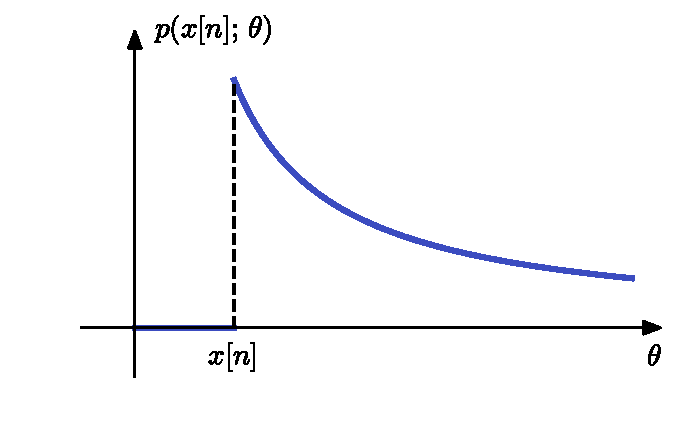
\includegraphics[width=\textwidth]{figuras/problem_3_1.pdf}
  \end{minipage}\hfill
  \begin{minipage}[c]{0.35\textwidth}
    \caption{
       Función de verosimilitud cuando \(x[n]\sim\mathcal{U}[0,\,\theta]\).
    } \label{fig:problem_3_1}
  \end{minipage}
\end{figure}
Para \(\theta>x[n]\) se tiene que \(p(x[n];\,\theta)=1/\theta\) y por lo tanto, 
\begin{align*}
 E\left[\frac{\partial\ln p(x[n];\,\theta)}{\partial\theta}\right]=
 E\left[\frac{\partial}{\partial\theta}\left(\ln \frac{1}{\theta}\right)\right]=
 E\left[\frac{\partial}{\partial\theta}\left(-\ln\theta\right)\right]=
 E\left[-\frac{1}{\theta}\right]=
 -\frac{1}{\theta}\neq0.
\end{align*}


\subsection{Problema 2}\label{sec:problem_3_2}

Se considera el caso en que se observa una única muestra
\[
 x[0]=A+w[0],
\]
donde \(w[0]\) tiene una PDF \(p(w[0])\) arbitraria y se desea estimar el parámetro \(A\). Mostrar que la CRLB para \(A\) es
\[
 \var(\hat{A})\geq\left[\int_{-\infty}^{\infty}\frac{\left(\dfrac{dp(u)}{du}\right)^2}{p(u)}\,du\right]^{-1}.
\]
Evaluar la CRLB en el caso en que la PDF es de Laplce, es decir,
\begin{equation}\label{eq:laplace_pdf}
 p(w[0])=\frac{1}{\sqrt{2}\sigma}\exp\left(-\frac{\sqrt{2}|w[0]|}{\sigma}\right),
\end{equation}
y comparar el resultado con el caso gaussiano.

\paragraph{Solución} La CRLB está dada por las ecuaciones \ref{eq:crlb_scalar} y \ref{eq:crlb_fisher_information}, por lo tanto hay que calcular la información de Fisher. En este caso,
\[
 x[0]=A+w[0],
\]
y como se obtuvo en el problema de la sección \ref{sec:problem_1_3}, la PDF de \(x[0]\) en términos de la PDF de \(w[0]\) es
\[
 p_{x[0]}(x[0];\,A)=p_{w[0]}(x[0]-A)=p(x[0]-A).
\]
Por lo tanto, hay que calcular
\[
 I(A)=-E\left[\frac{\partial^2\ln p(x[0]-A)}{\partial A^2}\right].
\]
Usando la regla de la cadena, se obtiene que la derivada primera es
\begin{equation}\label{eq:problem_3_2_tmp2}
 \frac{\partial\ln p(x[0]-A)}{\partial A}=\frac{1}{p(x[0]-A)}\frac{\partial p(x[0]-A)}{\partial A}(-1),
\end{equation}
y derivando nuevamente, se ve que
\begin{align}\label{eq:problem_3_2_tmp1}
 \frac{\partial^2\ln p(x[0]-A)}{\partial A^2}&=-\left\{\frac{-1}{p^2(x[0]-A)}\left[\frac{\partial p(x[0]-A)}{\partial A}\right]^2(-1)+
 \frac{1}{p(x[0]-A)}\frac{\partial^2 p(x[0]-A)}{\partial A^2}(-1)\right\}\nonumber\\
 &=-\frac{1}{p^2(x[0]-A)}\left[\frac{\partial p(x[0]-A)}{\partial A}\right]^2+
 \frac{1}{p(x[0]-A)}\frac{\partial^2 p(x[0]-A)}{\partial A^2}.
\end{align}
Para obtener la información de Fisher, hay que tomar la esperanza. Se demostrará que la esperanza del segundo sumando en la ecuación \ref{eq:problem_3_2_tmp1} es nula,
\begin{align*}
 E\left[\frac{1}{p(x[0]-A)}\frac{\partial^2 p(x[0]-A)}{\partial A^2}\right]
  &=\int\frac{1}{p(x[0]-A)}\frac{\partial^2 p(x[0]-A)}{\partial A^2}p(x[0]-A)\,dx[0]\\
  &=\int\frac{\partial^2 p(x[0]-A)}{\partial A^2}\,dx[0]\\
  &\overset{(a)}{=}\frac{\partial}{\partial A}\int\frac{\partial p(x[0]-A)}{\partial A}\,dx[0]\\
  &\overset{(b)}{=}-\frac{\partial}{\partial A}\int\frac{\partial \ln p(x[0]-A)}{\partial A}p(x[0]-A)\,dx[0]\\
  &=-\frac{\partial}{\partial A}E\left[\frac{\partial \ln p(x[0]-A)}{\partial A}\right]\\
  &\overset{(c)}{=}-\frac{\partial\,0}{\partial A}\\
  &=0,
\end{align*}
donde en \((a)\) se intercambió el orden de una derivada y la integración, en \((b)\) se sustituyó el integrando usando la ecuación \ref{eq:problem_3_2_tmp2} y en \((c)\) se observó que el término de la esperanza es la condición de regularidad y por lo tanto, es nula. Por lo tanto, al tomar la esperanza en la ecuación \ref{eq:problem_3_2_tmp1}, solo queda el primer sumando, y es
\begin{align}\label{eq:problem_3_2_tmp3}
 E\left[\frac{\partial^2\ln p(x[0]-A)}{\partial A^2}\right]
  &=-E\left\{\frac{1}{p^2(x[0]-A)}\left[\frac{\partial p(x[0]-A)}{\partial A}\right]^2\right\}\nonumber\\
  &=-\int\frac{1}{p^2(x[0]-A)}\left[\frac{\partial p(x[0]-A)}{\partial A}\right]^2p(x[0]-A)\,dx[0]\nonumber\\
  &=-\int\frac{1}{p(x[0]-A)}\left[\frac{\partial p(x[0]-A)}{\partial A}\right]^2\,dx[0]\nonumber\\
  &\overset{(a)}{=}-\int\frac{1}{p(x[0]-A)}\left[-\frac{\partial p(x[0]-A)}{\partial(x[0]-A)}\right]^2\,dx[0]\nonumber\\
  &\overset{(b)}{=}-\int\frac{1}{p(u)}\left[\frac{\partial p(u)}{\partial u}\right]^2\,du
\end{align}
donde en \((a)\) se usó la regla de la cadena de derivación para obtener que
\[
 \frac{\partial p(x[0]-A)}{\partial A}=
 \frac{\partial p(x[0]-A)}{\partial (x[0]-A)}\frac{\partial (x[0]-A)}{\partial A}
 =-\frac{\partial p(x[0]-A)}{\partial (x[0]-A)}
\]
y en \((b)\) se realizó el cambio de variable \(u=x[0]-A\) y por lo tanto, \(du=dx[0]\) y además se eliminó el signo de menos dentro del cuadrado.
De esta forma, se llegó a que
\[
 I(A)=-E\left[\frac{\partial^2\ln p(x[0]-A)}{\partial A^2}\right]=\int\frac{1}{p(u)}\left[\frac{\partial p(u)}{\partial u}\right]^2\,du,
\]
y por lo tanto,
\[
 \var(\hat{A})\geq\frac{1}{I(A)}=\left[\int_{-\infty}^{\infty}\frac{\left(\dfrac{dp(u)}{du}\right)^2}{p(u)}\,du\right]^{-1}.
\]
que es lo que se quería demostrar.

El mismo resultado puede obtenerse de forma un poco mas directa si se parte de la expresión alternativa de la información de Fisher dada por la igualdad de la ecuación \ref{eq:crlb_second_derivative_expectation},
\[
 I(A)=E\left[\left(\frac{\partial\ln p(x[0]-A)}{\partial A}\right)^2\right].
\]
Observando que la derivada primera ya se calculó en la ecuación \ref{eq:problem_3_2_tmp2}, se tiene que
\[
 I(A)=E\left[\left(\frac{\partial\ln p(x[0]-A)}{\partial A}\right)^2\right]=E\left\{\frac{1}{p^2(x[0]-A)}\left[\frac{\partial p(x[0]-A)}{\partial A}\right]^2\right\},
\]
y notando que la expresión dentro de la esperanza es igual al primer sumando de la ecuación \ref{eq:problem_3_2_tmp1}, la cual se calculó en la ecuación \ref{eq:problem_3_2_tmp3}, se llega al mismo resultado.

En el caso en que la PDF de \(w[0]\) es Laplaciana, se tiene que
\[
 p(u)=\frac{1}{\sqrt{2}\sigma}\exp\left(-\frac{\sqrt{2}u}{\sigma}\right),\qquad u\geq 0,\textrm{ par},
\]
y la derivada es
\[
 \frac{dp(u)}{du}=\frac{1}{\sqrt{2}\sigma}\left(-\frac{\sqrt{2}}{\sigma}\right)\exp\left(-\frac{\sqrt{2}u}{\sigma}\right)
 =-\frac{1}{\sigma^2}\exp\left(-\frac{\sqrt{2}u}{\sigma}\right),\qquad u\geq 0,
\]
la cual es impar, ya que la derivada de una función par es impar.
Por lo tanto, usando el resultado anterior, se tiene que
\begin{align*}
 I(A)&=\int_{-\infty}^{\infty}\frac{1}{p(u)}\left[\frac{dp(u)}{du}\right]^2\,du\\
  &\overset{(a)}{=}2\int_{0}^{\infty}\frac{\sqrt{2}\sigma}{\exp\left(-\dfrac{\sqrt{2}u}{\sigma}\right)}\frac{1}{\sigma^4}\left[\exp\left(-\frac{\sqrt{2}u}{\sigma}\right)\right]^2\,du\\
  &=\frac{2\sqrt{2}}{\sigma^3}\int_{0}^{\infty}\exp\left(-\frac{\sqrt{2}u}{\sigma}\right)\,du\\
  &=\frac{2\sqrt{2}}{\sigma^3}\left[-\frac{\sigma}{\sqrt{2}}\exp\left(-\frac{\sqrt{2}u}{\sigma}\right)\bigg|_{0}^{\infty}\right]\\
  &=-\frac{2}{\sigma^2}\left(0-1\right)\\
  &=\frac{2}{\sigma^2},
\end{align*}
donde en \((a)\) se consideró que el integrando es una función par, ya que \(1/p(u)\) es par por ser \(p(u)\) par y el cuadrado de la derivada de \(p(u)\) también es par por ser la derivada impar. De esta forma, se obtiene que
\[
 \var(\hat{A})\geq\frac{1}{I(A)}=\frac{\sigma^2}{2}.
\]
Puede demostrarse que el parámetro \(\sigma\) en la PDF de Laplace (ecuación \ref{eq:laplace_pdf}) es la desviación estándar, es decir, \(\var(w[0])=\sigma^2\).
En el ejemplo 3.2 de \cite{kay93fundamentals} se demuestra que si \(w[0]\sim\mathcal{N}(0,\,\sigma^2)\), la CRLB de \(\hat{A}\) es
\[
 \var(\hat{A})\geq\sigma^2.
\]
Se concluye que la CRLB es la mitad en el caso en que el ruido es de Laplace respecto al caso en que el ruido es gaussiano. Puede demostrarse que el ruido gaussiano es el que produce la mayor CRLB \cite{stoica2011gaussian}.

\subsection{Problema 3}\label{sec:problem_3_3}

Se observan los datos \(x[n]=Ar^n+w[n]\) para \(n=0,\dots,\,N-1\), donde \(w[n]\) es WGN con varianza \(\sigma^2\) y \(r>0\) es conocido. Encontrar la CRLB para \(A\). Mostrar que existe un estimador eficiente y encontrar su varianza. Indicar que ocurre cuando \(N\to\infty\) discutiendo según el valor de \(r\).

\paragraph{Solución} 

La CRLB del parámetro \(A\) puede calcularse directamente empleando la ecuación \ref{eq:crlb_general_signal_wgn}, pero se realizará el razonamiento completo ya que conviene tener calculada la derivada primera de la función de verosimilitud logarítmica para el estudio de la eficiencia.

La PDF de los datos es
\[
 p(\x;\,A)=\frac{1}{(2\pi\sigma^2)^\frac{N}{2}}\exp\left\{-\frac{1}{2\sigma^2}\sum_{n=0}^{N-1}(x[n]-Ar^n)^2\right\}
\]
por lo que la función de verosimilitud logarítmica queda
\[
 \ln p(\x;\,A)=-\frac{N}{2}\ln(2\pi\sigma^2)-\frac{1}{2\sigma^2}\sum_{n=0}^{N-1}(x[n]-Ar^n)^2.
\]
Diferenciando una vez se obtiene que
\begin{align}\label{eq:problem_3_3_likelihood_derivative}
 \frac{\partial\ln p(\x;\,A)}{\partial A}&=\frac{1}{\sigma^2}\sum_{n=0}^{N-1}(x[n]-Ar^n)r^n\nonumber\\
  &=\frac{1}{\sigma^2}\sum_{n=0}^{N-1}x[n]r^n-\frac{A}{\sigma^2}\sum_{n=0}^{N-1}r^{2n},
\end{align}
y diferenciando nuevamente se llega a que
\[
 \frac{\partial^2\ln p(\x;\,A)}{\partial A^2}=-\frac{1}{\sigma^2}\sum_{n=0}^{N-1}r^{2n}.
\]
Se concluye que la información de Fisher de \(A\) es
\[
 I(A)=-E\left[\frac{\partial^2\ln p(\x;\,A)}{\partial A^2}\right]=\frac{1}{\sigma^2}\sum_{n=0}^{N-1}r^{2n},
\]
por lo que la CRLB es
\[
 \var(\hat{A})\geq\dfrac{\sigma^2}{\displaystyle\sum_{n=0}^{N-1}r^{2n}}.
\]
Para estudiar si existe un estimador eficiente, hay que ver si es posible factorizar la ecuación \ref{eq:problem_3_3_likelihood_derivative} como la ecuación \ref{eq:crlb_efficiency_condition}. Efectivamente, se observa que la ecuación \ref{eq:problem_3_3_likelihood_derivative} puede expresarse como
\[
 \frac{\partial\ln p(\x;\,A)}{\partial A}=\frac{1}{\sigma^2}\sum_{n=0}^{N-1}r^{2n}\left(\dfrac{\displaystyle\sum_{n=0}^{N-1}x[n]r^n}{\displaystyle\sum_{n=0}^{N-1}r^{2n}}-A\right)=I(A)(g(\x)-A),
\]
concluyendo que el estimador eficiente de \(A\) es
\[
 \hat{A}=\dfrac{\displaystyle\sum_{n=0}^{N-1}x[n]r^n}{\displaystyle\sum_{n=0}^{N-1}r^{2n}}
\]
cuya varianza es \(1/I(A)\).

Se estudiará a continuación el límite de la varianza cuando \(N\to\infty\). Considerando que para \(r>0\)
\[\def\arraystretch{2}
 \sum_{n=0}^{N-1}r^{2n}=
 \left\{\begin{array}{ll}
  \dfrac{1-r^{2N}}{1-r^2}, &  \textrm{si }r\neq 1\\
  N, &  \textrm{si }r=1,
 \end{array}\right.
\]
se tiene que
\[\def\arraystretch{2}
 \var(\hat{A})=\dfrac{\sigma^2}{\displaystyle\sum_{n=0}^{N-1}r^{2n}}=
 \left\{\begin{array}{ll}
  \dfrac{\sigma^2(1-r^2)}{1-r^{2N}}, &  \textrm{si }r\neq 1\\
  \dfrac{\sigma^2}{N}, &  \textrm{si }r=1.
 \end{array}\right.
\]
Por lo tanto, si \(r\neq1\), el límite es
\[\def\arraystretch{2}
 \lim_{N\to\infty}\var(\hat{A})=\lim_{N\to\infty}\frac{\sigma^2(1-r^2)}{1-r^{2N}}=
 \left\{\begin{array}{ll}
  \sigma^2(1-r^2), &  \textrm{si }0<r<1\\
  0, &  \textrm{si }r>1.
 \end{array}\right.
\]
y como en el caso con \(r=1\) el límite es cero, se concluye que
\[\def\arraystretch{2}
 \lim_{N\to\infty}\var(\hat{A})=
 \left\{\begin{array}{ll}
  \sigma^2(1-r^2), &  \textrm{si }0<r<1\\
  0, &  \textrm{si }r\geq1.
 \end{array}\right.
\]

\subsection{Problema 4} 

Se observa \(x[n]=r^n+w[n]\) para \(n=0,\dots,\,N-1\), donde \(w[n]\) es WGN con varianza \(\sigma^2\) y \(r\) es el parámetro desconocido a estimar. Encontrar la CRLB para \(A\). Si existe un estimador eficiente, encontrar su varianza.

\paragraph{Solución} 

La PDF de los datos es
\[
 p(\x;\,r)=\frac{1}{(2\pi\sigma^2)^\frac{N}{2}}\exp\left\{-\frac{1}{2\sigma^2}\sum_{n=0}^{N-1}(x[n]-r^n)^2\right\}
\]
y la función de verosimilitud logarítmica queda
\[
 \ln p(\x;\,r)=-\frac{N}{2}\ln(2\pi\sigma^2)-\frac{1}{2\sigma^2}\sum_{n=0}^{N-1}(x[n]-r^n)^2.
\]
Diferenciando una vez se obtiene que
\begin{align*}
 \frac{\partial\ln p(\x;\,r)}{\partial r}&=\frac{1}{\sigma^2}\sum_{n=0}^{N-1}(x[n]-r^n)nr^{n-1}\\
  &=\frac{1}{\sigma^2}\sum_{n=0}^{N-1}n(x[n]r^{n-1}-r^{2n-1}).
\end{align*}
Puede verse que la derivada no puede factorizarse como
\[
 \frac{\partial\ln p(\x;\,r)}{\partial r}=I(r)\left(g(\x)-r\right)
\]
y por lo tanto, no existe un estimador eficiente. Diferenciando nuevamente se llega a que
\[
 \frac{\partial^2\ln p(\x;\,r)}{\partial r^2}=\frac{1}{\sigma^2}\sum_{n=0}^{N-1}n\left[x[n](n-1)r^{n-2}-(2n-1)r^{2n-2}\right]
\]
y tomando esperanza se obtiene que
\begin{align*}
 E\left[\frac{\partial^2\ln p(\x;\,r)}{\partial r^2}\right]&=\frac{1}{\sigma^2}\sum_{n=0}^{N-1}n\left[E(x[n])(n-1)r^{n-2}-(2n-1)r^{2n-2}\right]\\
  &\overset{(a)}{=}\frac{1}{\sigma^2}\sum_{n=0}^{N-1}n\left[(n-1)r^{2n-2}-(2n-1)r^{2n-2}\right]\\
  &=-\frac{1}{\sigma^2}\sum_{n=0}^{N-1}n^2r^{2n-2},
\end{align*}
donde en \((a)\) se empleó que \(E(x[n])=r^n\).
Se concluye que la CRLB es
\[
 \var(\hat{r})\geq\dfrac{\sigma^2}{\displaystyle\sum_{n=0}^{N-1}n^2r^{2n-2}}.
\]
Nuevamente el resultado se podría haber obtenido directamente usando la ecuación \ref{eq:crlb_general_signal_wgn}.

\subsection{Problema 5}\label{sec:problem_3_5} 

Se observa \(x[n]=A+w[n]\) para \(n=0,\dots,\,N-1\), donde \(\w=[w[0]\,w[1]\dots w[N-1]]^T\sim\mathcal{N}(\mathbf{0},\C)\). Encontrar la CRLB para \(A\). Si existe un estimador eficiente, encontrar su varianza.

\paragraph{Solución} 

La PDF de los datos es
\[
 p(\x,\,A)=\frac{1}{(2\pi)^\frac{N}{2}\det^{\frac{1}{2}}(\C)}\exp\left\{-\frac{1}{2}(\x-A\mathbf{1})^T\C^{-1}(\x-A\mathbf{1})\right\},
\]
donde \(\mathbf{1}=[1\,1\dots 1]^T\) de tamaño \(N\times1\). Tomando el logaritmo, se tiene que
\[
 \ln p(\x,\,A)=-\frac{N}{2}\ln(2\pi)-\frac{1}{2}\ln\det(\C)-\frac{1}{2}(\x-A\mathbf{1})^T\C^{-1}(\x-A\mathbf{1}).
\]
y diferenciando, se observa que
\begin{align*}
 \frac{\partial \ln p(\x,\,A)}{\partial A}&=-\frac{1}{2}\frac{\partial}{\partial A}\left[(\x-A\mathbf{1})^T\C^{-1}(\x-A\mathbf{1})\right]\\
   &=-\frac{1}{2}\frac{\partial}{\partial A}\left[\x^T\C^{-1}\x-A\x^T\C^{-1}\mathbf{1}-A\mathbf{1}^T\C^{-1}\x+A^2\mathbf{1}^T\C^{-1}\mathbf{1}\right]\\
   &=-\frac{1}{2}\frac{\partial}{\partial A}\left[\x^T\C^{-1}\x-2A\mathbf{1}^T\C^{-1}\x+A^2\mathbf{1}^T\C^{-1}\mathbf{1}\right]\\
   &=-\frac{1}{2}\left[-2\mathbf{1}^T\C^{-1}\x+2A\mathbf{1}^T\C^{-1}\mathbf{1}\right]\\
   &=\mathbf{1}^T\C^{-1}\x-A\mathbf{1}^T\C^{-1}\mathbf{1},
\end{align*}
que se puede expresar como
\[
 \frac{\partial \ln p(\x,\,A)}{\partial A}=\mathbf{1}^T\C^{-1}\mathbf{1}\left[\frac{\mathbf{1}^T\C^{-1}\x}{\mathbf{1}^T\C^{-1}\mathbf{1}}-A\right].
\]
Comparando con la ecuación \ref{eq:crlb_efficiency_condition} se tiene que
\[
 \hat{A}=\frac{\mathbf{1}^T\C^{-1}\x}{\mathbf{1}^T\C^{-1}\mathbf{1}}\qquad\qquad
 I(A)=\mathbf{1}^T\C^{-1}\mathbf{1}.
\]
Se concluye que el estimador \(\hat{A}\) es eficiente y su varianza es \(1/I(A)\).

\subsection{Problema 6} 

Se consideran dos observaciones \(x[0]\) y \(x[1]\) independientes con PDF
\[
 x[0]\sim\mathcal{N}(\theta,\,1)\qquad\qquad
 x[1]\sim
 \left\{\begin{array}{ll}
  \mathcal{N}(\theta,\,1), &  \textrm{si }\theta\geq0\\
  \mathcal{N}(\theta,\,2), &  \textrm{si }\theta<0.
 \end{array}\right.
\]
Calcular la CRLB del parámetro \(\theta\).

\paragraph{Solución}

La PDF de cada observación es
\[
 p(x[0];\,\theta)=\frac{1}{\sqrt{2\pi}}\exp\left\{-\frac{1}{2}(x[0]-\theta)^2\right\}
 \qquad
 \def\arraystretch{2}
 p(x[1];\,\theta)=
 \left\{\begin{array}{ll}
  \dfrac{1}{\sqrt{2\pi}}\exp\left\{-\dfrac{1}{2}(x[1]-\theta)^2\right\}, &  \textrm{si }\theta\geq0\\
  \dfrac{1}{\sqrt{4\pi}}\exp\left\{-\dfrac{1}{4}(x[1]-\theta)^2\right\}, &  \textrm{si }\theta<0.
 \end{array}\right.
\]
Por lo tanto, la PDF de \(\x\) es
\[
 \def\arraystretch{2}
 p(\x;\,\theta)=p(x[0];\,\theta)p(x[1];\,\theta)=
 \left\{\begin{array}{ll}
  \dfrac{1}{2\pi}\exp\left\{-\dfrac{1}{2}(x[0]-\theta)^2-\dfrac{1}{2}(x[1]-\theta)^2\right\}, &  \textrm{si }\theta\geq0\\
  \dfrac{1}{2\sqrt{2}\pi}\exp\left\{-\dfrac{1}{2}(x[0]-\theta)^2-\dfrac{1}{4}(x[1]-\theta)^2\right\}, &  \textrm{si }\theta<0,
 \end{array}\right.
\]
y al tomar el logaritmo se obtiene que
\[
 \def\arraystretch{2}
 \ln p(\x;\,\theta)=
 \left\{\begin{array}{ll}
  -\ln(2\pi)-\dfrac{1}{2}(x[0]-\theta)^2-\dfrac{1}{2}(x[1]-\theta)^2, &  \textrm{si }\theta\geq0\\
  -\ln(2\sqrt{2}\pi)-\dfrac{1}{2}(x[0]-\theta)^2-\dfrac{1}{4}(x[1]-\theta)^2, &  \textrm{si }\theta<0.
 \end{array}\right.
\]
Diferenciando respecto al parámetro, se obtiene que
\[
 \def\arraystretch{2}
 \frac{\partial\ln p(\x;\,\theta)}{\partial\theta}=
 \left\{\begin{array}{ll}
  (x[0]-\theta)+(x[1]-\theta), &  \textrm{si }\theta\geq0\\
  (x[0]-\theta)+\dfrac{1}{2}(x[1]-\theta), &  \textrm{si }\theta<0
 \end{array}\right.
 =
 \left\{\begin{array}{ll}
  x[0]+x[1]-2\theta, &  \textrm{si }\theta\geq0\\
  x[0]+\dfrac{1}{2}x[1]-\dfrac{3}{2}\theta, &  \textrm{si }\theta<0,
 \end{array}\right.
\]
y diferenciando nuevamente se llega a que
\[
 \def\arraystretch{2}
 \frac{\partial^2\ln p(\x;\,\theta)}{\partial\theta^2}=
 \left\{\begin{array}{ll}
  -2, &  \textrm{si }\theta\geq0\\
  -\dfrac{3}{2}, &  \textrm{si }\theta<0.
 \end{array}\right.
\]
Por lo tanto, la información de Fisher es
\[
 \def\arraystretch{2}
 I(\theta)=-E\left[\frac{\partial^2\ln p(\x;\,\theta)}{\partial\theta^2}\right]=
 \left\{\begin{array}{ll}
   2, &  \textrm{si }\theta\geq0\\
  \dfrac{3}{2}, &  \textrm{si }\theta<0,
 \end{array}\right.
\]
concluyendo que la CBRL es
\[
 \def\arraystretch{2}
 \var(\hat{\theta})\geq\frac{1}{I(\theta)}=
 \left\{\begin{array}{ll}
   \dfrac{1}{2}, &  \textrm{si }\theta\geq0\\
  \dfrac{2}{3}, &  \textrm{si }\theta<0.
 \end{array}\right.
\]

\subsection{Problema 7}\label{sec:problem_3_7}

Probar que
\[
 \frac{1}{N}\sum_{n=0}^{N-1}\cos(4\pi f_0n+2\phi)\approx0,
\]
resultado empleado en el ejemplo 3.4. ¿Qué condiciones se requieren sobre \(f_0\) para que el resultado se cumpla?

\paragraph{Solución} Defínase \(\alpha=4\pi f_0\) y \(\beta=2\phi\) y se obsérvese que
\begin{align*}
 \sum_{n=0}^{N-1}\cos(\alpha n+\beta)&=\operatorname{Re}\left[\sum_{n=0}^{N-1}e^{j(\alpha n+\beta)}\right]\\
  &=\operatorname{Re}\left[e^{j\beta}\sum_{n=0}^{N-1}e^{j\alpha n}\right]\\
  &=\operatorname{Re}\left[e^{j\beta}\frac{1-e^{j\alpha N}}{1-e^{j\alpha}}\right]\\
  &=\operatorname{Re}\left[e^{j\beta}\frac{e^{j\alpha N/2}}{e^{j\alpha/2}}\frac{e^{-j\alpha N/2}-e^{j\alpha N/2}}{e^{-j\alpha/2}-e^{j\alpha/2}}\right]\\
  &=\operatorname{Re}\left[e^{j\beta}e^{j\alpha(N-1)/2}\frac{\sin(\alpha N/2)}{\sin(\alpha/2)}\right]\\
  &=\operatorname{Re}\left\{\left[\cos(\alpha(N-1)/2+\beta)+j\sin(\alpha(N-1)/2+\beta)\right]\frac{\sin(\alpha N/2)}{\sin(\alpha/2)}\right\}\\
  &=\cos[\alpha(N-1)/2+\beta]\frac{\sin(\alpha N/2)}{\sin(\alpha/2)},
\end{align*}
y por lo tanto,
\[
 \frac{1}{N}\sum_{n=0}^{N-1}\cos(4\pi f_0n+2\phi)=\frac{\sin(2\pi f_0 N)}{N\sin(2\pi f_0)}\cos[2\pi f_0(N-1)+2\phi].
\]
En la figura \ref{fig:problem_3_7} se grafica \(|\sin(2\pi f_0 N)/(N\sin(2\pi f_0))|\) para \(N=20\). Esta función es periódica de período \(1/2\). Como se observa en la figura, se cumple que
\[
 \left|\frac{1}{N}\sum_{n=0}^{N-1}\cos(4\pi f_0n+2\phi)\right|\leq\left|\frac{\sin(2\pi f_0 N)}{N\sin(2\pi f_0)}\right|\approx0
\]
si \(f_0\) no está cercan a 0 o a 1/2, y la aproximación es mejor para \(f_0\) en torno a 1/4. Además, la aproximación mejora al incrementar \(N\).
\begin{figure}[!htb]
\begin{center}
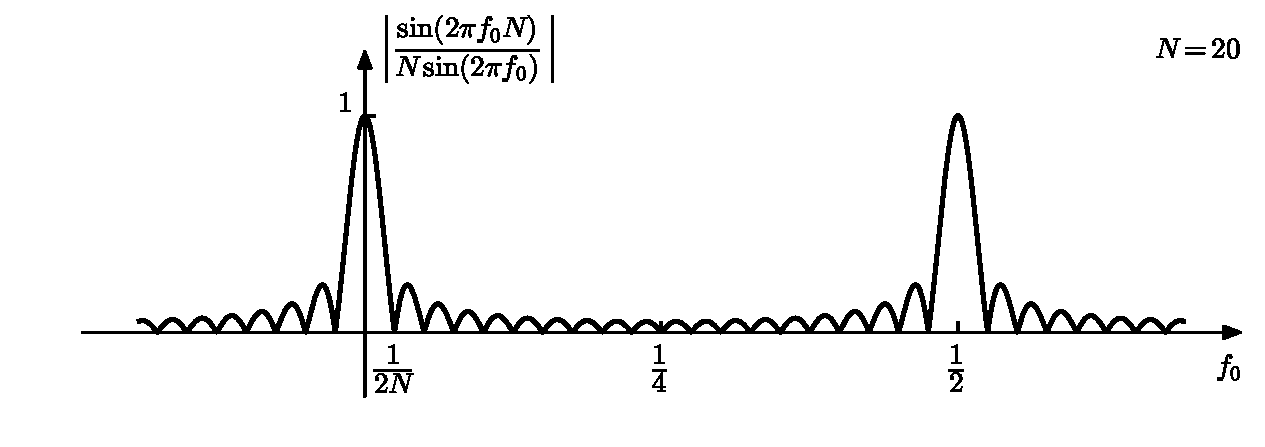
\includegraphics[width=0.92\textwidth]{figuras/problem_3_7.pdf}
\caption{\label{fig:problem_3_7} Gráfica de \(|\sin(2\pi f_0 N)/(N\sin(2\pi f_0))|\) para \(N=20\). La función es periódica de período \(1/2\) y los ceros se encuentran en \(f_0=k/(2N)\). Como se observa, la función toma valores pequeños si \(f_0\) no está cerca de 0 o 1/2. Además, la función decrece al incrementar \(N\).}
\end{center}
\end{figure}

Notar además que
\begin{align*}
 \sum_{n=0}^{N-1}\sin(\alpha n+\beta)&=\operatorname{Im}\left[\sum_{n=0}^{N-1}e^{j(\alpha n+\beta)}\right]\\
  &=\sin[\alpha(N-1)/2+\beta]\frac{\sin(\alpha N/2)}{\sin(\alpha/2)},
\end{align*}


\subsection{Problema 8}\label{sec:problem_3_8} 

Para el problema de estimación del nivel de DC en WGN (ver sección \ref{sec:problema_1_4}), calcular la CRLB empleando la expresión alternativa 
\[
 \var(\hat{\theta})\geq\dfrac{1}{E\left[\left(\dfrac{\partial\ln p(\x;\,\theta)}{\partial\theta}\right)^2\right]},
\]
que proviene de las ecuaciones \ref{eq:crlb_scalar}, \ref{eq:crlb_fisher_information} y \ref{eq:crlb_second_derivative_expectation}.

\paragraph{Solución} En el problema de la estimación del nivel de DC en WGN, se tienen las observaciones
\[
 x[n]=A+w[n]\qquad n=0,\,1,\dots,\,N-1,
\]
donde \(w[n]\) es WGN con varianza \(\sigma^2\) y se quiere determinar la CRLB para A. Como se explica en el ejemplo 3.3 de \cite{kay93fundamentals}, la PDF de los datos es
\begin{align}\label{eq:dc_in_wgn_pdf}
 p(\x;\,A)&=\prod_{n=0}^{N-1}\frac{1}{\sqrt{2\pi\sigma^2}}\exp\left[-\frac{1}{2\sigma^2}(x[n]-A)^2\right]\nonumber\\
  &=\frac{1}{(2\pi\sigma^2)^\frac{N}{2}}\exp\left[-\frac{1}{2\sigma^2}\sum_{n=0}^{N-1}(x[n]-A)^2\right],
\end{align}
y al tomar el logaritmo, se obtiene que
\[
 \ln p(\x;\,A)=-\frac{N}{2}\ln(2\pi\sigma^2)-\frac{1}{2\sigma^2}\sum_{n=0}^{N-1}(x[n]-A)^2.
\]
Diferenciando respecto al parámetro, se llega a que
\begin{equation}\label{eq:dc_in_wgn_pdf_first_derivative}
 \frac{\partial\ln p(\x;\,A)}{\partial A}=\frac{1}{\sigma^2}\sum_{n=0}^{N-1}(x[n]-A).
\end{equation}
La información de Fisher es
\begin{align*}
 I(A)=E\left[\left(\dfrac{\partial\ln p(\x;\,\theta)}{\partial\theta}\right)^2\right]&=
  E\left\{\left[\frac{1}{\sigma^2}\sum_{n=0}^{N-1}(x[n]-A)\right]^2\right\}\\
  &=E\left\{\frac{1}{\sigma^4}\left[\sum_{m=0}^{N-1}(x[m]-A)\right]\left[\sum_{n=0}^{N-1}(x[n]-A)\right]\right\}\\
  &=E\left[\frac{1}{\sigma^4}\sum_{m=0}^{N-1}\sum_{n=0}^{N-1}(x[m]-A)(x[n]-A)\right]\\
  &=\frac{1}{\sigma^4}\sum_{m=0}^{N-1}\sum_{n=0}^{N-1}E\left[(x[m]-A)(x[n]-A)\right]\\
  &\overset{(a)}{=}\frac{1}{\sigma^4}\sum_{m=0}^{N-1}\sum_{n=0}^{N-1}\sigma^2\delta[m-n]\\
  &=\frac{1}{\sigma^4}\sum_{n=0}^{N-1}\sigma^2\\
  &=\frac{N}{\sigma^2},
\end{align*}
donde en \((a)\) se empleó que
\begin{align*}
 E\left[(x[m]-A)(x[n]-A)\right]&=
 \def\arraystretch{2}
 \left\{\begin{array}{ll}
  E\left[(x[n]-A)^2\right]=\sigma^2, &  \textrm{si }m=n\\
  E\left[(x[m]-A)\right]E\left[(x[n]-A)\right]=0, &  \textrm{si }m\neq m
 \end{array}\right.\\
  &=\sigma^2\delta[m-n].
\end{align*}
Se concluye que
\[
 \var(\hat{\theta})\geq\dfrac{\sigma^2}{N}.
\]

Otra forma de ver lo mismo empleando resultados anteriores, es notando que la ecuación \ref{eq:dc_in_wgn_pdf_first_derivative} puede escribirse como
\begin{align*}
 \frac{\partial\ln p(\x;\,A)}{\partial A}&=\frac{1}{\sigma^2}\sum_{n=0}^{N-1}(x[n]-A)\\
   &=\frac{1}{\sigma^2}\left(\sum_{n=0}^{N-1}x[n]-NA\right)\\
   &=\frac{1}{\sigma^2}\left(N\bar{\x}-NA\right)\\
   &=\frac{N}{\sigma^2}\left(\bar{\x}-A\right),
\end{align*}
y al elevar al cuadrado y tomar esperanza, se tiene que
\begin{align*}
 I(A)=E\left[\left(\dfrac{\partial\ln p(\x;\,\theta)}{\partial\theta}\right)^2\right]&=
  \frac{N^2}{\sigma^4}E\left[\left(\bar{\x}-A\right)^2\right]\\
   &\overset{(a)}{=}\frac{N^2}{\sigma^4}\var(\bar{\x})\\
   &\overset{(b)}{=}\frac{N^2}{\sigma^4}\frac{\sigma^2}{N}\\
   &=\frac{N}{\sigma^2},
\end{align*}
donde en \((a)\) y en \((b)\) se empleó que \(\bar{\x}\sim\mathcal{N}(A,\,\sigma^2/N)\), como se demostró el la sección \ref{sec:problem_2_3}.

\subsection{Problema 9}\label{sec:problem_3_9}

Se observan dos muestras de un nivel de DC en ruido gaussiano \emph{correlacionado},
\begin{align*}
 x[0]&=A+w[0]\\
 x[1]&=A+w[1],
\end{align*}
donde \(\w=[w[0]\,w[1]]^T\) tiene media nula y matriz de covarianza
\[
 \C=\sigma^2
 \begin{bmatrix}
    1 & \rho\\
    \rho & 1
 \end{bmatrix}.
\]
El parámetro \(\rho\) es el coeficiente de correlación entre \(w[0]\) y \(w[1]\). Calcular la CRLB de \(A\) y comparar con el caso en que \(w[n]\) es WGN, es decir, cuando \(\rho=0\). Además explicar que ocurre cuando \(\rho\to\pm1\). Finalmente, comentar sobre la propiedad de aditividad de la información de Fisher para observaciones no independientes.

\paragraph{Solución} 

La CRLB para el caso general de ruido gaussiano ya fue resuelto en el problema de la sección \ref{sec:problem_3_5}, por lo que podrían emplearse los resultados obtenidos allí. También podría obtenerse la información de Fisher de forma inmediata a partir de la ecuación \ref{eq:crlb_general_gaussian_scalar}, pero se harán las cuentas nuevamente para este caso particular.

La PDF de los datos es
\[
 p(\x,\,A)=\frac{1}{2\pi\sqrt{\det(\C)}}\exp\left\{-\frac{1}{2}(\x-A\mathbf{1})^T\C^{-1}(\x-A\mathbf{1})\right\},
\]
donde \(\mathbf{1}=[1\,1]^T\). 
El determinante de la matriz de correlación es
\[
 \det(\C)=\sigma^4(1-\rho^2)
\]
y la inversa de la matriz de correlación es
\[
 \C^{-1}=\frac{1}{\sigma^2(1-\rho^2)}
 \begin{bmatrix}
    1 & -\rho\\
    -\rho & 1
 \end{bmatrix}.
\]
Además,
\[
 \C^{-1}(\x-A\mathbf{1})=\frac{1}{\sigma^2(1-\rho^2)}
 \begin{bmatrix}
    1 & -\rho\\
    -\rho & 1
 \end{bmatrix}
 \begin{bmatrix}
    x[0]-A\\
    x[1]-A
 \end{bmatrix}
 =\frac{1}{\sigma^2(1-\rho^2)}
 \begin{bmatrix}
    (x[0]-A)-\rho(x[1]-A)\\
    -\rho(x[0]-A)+(x[1]-A)
 \end{bmatrix}
\]
y
\begin{align*}
  (\x-A\mathbf{1})^T\C^{-1}(\x-A\mathbf{1})&=\frac{1}{\sigma^2(1-\rho^2)}
 \begin{bmatrix}
     x[0]-A & x[1]-A 
 \end{bmatrix}
 \begin{bmatrix}
    (x[0]-A)-\rho(x[1]-A)\\
    -\rho(x[0]-A)+(x[1]-A)
 \end{bmatrix}\\
 &=\frac{(x[0]-A)^2-2\rho(x[0]-A)(x[1]-A)+(x[1]-A)^2}{\sigma^2(1-\rho^2)}.
\end{align*}
Por lo tanto, la PDF de los datos en este caso queda
\[
 p(\x,\,A)=\frac{1}{2\pi\sigma^2\sqrt{(1-\rho^2)}}\exp\left\{-\frac{(x[0]-A)^2-2\rho(x[0]-A)(x[1]-A)+(x[1]-A)^2}{2\sigma^2(1-\rho^2)}\right\},
\]
y tomando el logaritmo, se obtiene que
\[
 \ln p(\x,\,A)=-\ln2\pi\sigma^2\sqrt{(1-\rho^2)}-\frac{(x[0]-A)^2-2\rho(x[0]-A)(x[1]-A)+(x[1]-A)^2}{2\sigma^2(1-\rho^2)}.
\]
Al diferenciar respecto al parámetro se observa que
\begin{align*}
 \frac{\partial \ln p(\x,\,A)}{\partial A}&=-\frac{-2(x[0]-A)-2\rho[-(x[0]-A)-(x[1]-A)]-2(x[1]-A)}{2\sigma^2(1-\rho^2)}\\
 &=\frac{x[0]+x[1]-2A-\rho(x[0]+x[1]-2A)}{\sigma^2(1-\rho^2)}\\
 &=\frac{(x[0]+x[1]-2A)(1-\rho)}{\sigma^2(1-\rho^2)},
\end{align*}
que puede expresarse como
\[
 \frac{\partial \ln p(\x,\,A)}{\partial A}=\frac{2}{\sigma^2(1+\rho)}\left(\frac{x[0]+x[1]}{2}-A\right),
\]
donde se tuvo en cuenta que \((1-\rho^2)=(1+\rho)(1-\rho)\).
Como la derivada de la función de verosimilitud se factorizó como indica la ecuación \ref{eq:crlb_efficiency_condition}, se concluye que el estimador media muestral
\[
 \hat{A}=\frac{x[0]+x[1]}{2},
\]
es eficiente y la información de Fisher es
\begin{equation}\label{eq:problem_3_3_fisher_info}
 I(A)=\frac{2}{\sigma^2(1+\rho)}.
\end{equation}
Por lo tanto, la CRLB de \(A\) es
\[
 \var(\hat{A})\geq\frac{\sigma^2}{2}(1+\rho).
\]

El coeficiente de correlación entre dos variables aleatorias \(x\) e \(y\) es una medida de la dependencia entre las variables aleatorias (ver el capítulo 6 de \cite{papoulis2002probability}) y se define como
\[
 \rho_{xy}=\frac{C_{xy}}{\sigma_x\sigma_y}.
\]
Se cumple que \(-1\leq\rho_{xy}\leq1\). En el caso en que \(\rho_{xy}=0\), la covarianza es nula y las variables son no correlacionadas, ya que
\[
 C_{xy}=E(xy)-E(x)E(y)=0\qquad\Rightarrow\qquad E(xy)=E(x)E(y).
\]
En el caso en que \(\rho_{xy}=1\), las variables aleatorias tienen dependencia lineal, \(y=ax\), donde \(a\) es una constante. De esta forma,
\[
 \rho_{xy}=\frac{C_{xy}}{\sigma_x\sigma_y}=\frac{E(xy)-E(x)E(y)}{\sigma_x\sigma_y}
 =\frac{aE(x^2)-aE^2(x)}{a\sigma^2_x}=\frac{a\sigma^2_x}{a\sigma^2_x}=1,
\]
donde se empleó que si \(y=ax\) se cumple que \(\sigma_y=a\sigma_x\). En el caso en que las variables aleatorias tienen la misma varianza y \(\rho=1\), se cumple que \(y=x\), y en el caso en que \(\rho=-1\), se cumple que \(y=-x\). Volviendo a la CRLB de \(A\), en el caso en que \(\rho=0\) se cumple que
\[
 \var(\hat{A})\geq\frac{\sigma^2}{2},
\]
que es la CRLB calculada previamente para el caso de WGN con \(N=2\). En el caso en que \(\rho\to1\)
\[
 \var(\hat{A})\geq\sigma^2,
\]
que es la CRLB al observar una única muestra. Esto se debe a que como \(\rho\to1\), \(w[1]=w[0]\) y por lo tanto, se dispone de una única muestra independiente. En el caso en que \(\rho\to-1\), se cumple que
\[
 \var(\hat{A})\geq0,
\]
y de hecho, la media muestral es
\[
 \hat{A}=\frac{x[0]+x[1]}{2}=\frac{A+w[0]+A-w[0]}{2}=A,
\]
es decir, el valor exacto del parámetro para cualquier realización de las muestras de ruido.

La información de Fisher en el caso de una sola muestra es
\[
 i(A)=\frac{1}{\sigma^2}.
\]
La propiedad de aditividad de la información de Fisher se cumple en el caso de muestras no correlacionadas. Efectivamente, de la ecuación \ref{eq:problem_3_3_fisher_info} se observa que en el caso en que \(\rho=0\), se cumple que
\[
 I(A)=\frac{2}{\sigma^2}=2i(A).
\]
Además, se observa que
\[
 i(A)\leq I(A)\leq\infty,
\]
donde la cota inferior se da en el caso en que \(\rho=1\) (muestras completamente correlacionadas) y el límite superior se da en el caso en que \(\rho=-1\). Cuando las muestras están correlacionadas con \(0\leq\rho\leq1\) se cumple que
\[
 i(A)\leq I(A)\leq 2i(A),
\]
y en general, si las muestras están correlacionadas con \(\rho>0\) se cumple que
\[
 I(A)\leq Ni(A).
\]

\subsection{Problema 10}\label{sec:problem_3_10} 

Usando la ecuación \ref{eq:crlb_fisher_information_matrix_alt}, probar que la matriz de información de Fisher es semidefinida positiva para todo \(\thetabf\). En la práctica se asumirá que es positiva definida y por lo tanto invertible, aunque no sea siempre el caso. Considerar el modelo de los datos del problema de la sección \ref{sec:problem_3_3} con la modificación de que ahora \(r\) también es desconocido. Calcular la matriz de información de Fisher de \(\thetabf=[A\,r]^T\). ¿Existen valores de \(\thetabf\) tal que \(\I(\thetabf)\) no es definida positiva?

\paragraph{Solución} 

Una matriz \(\mathbf{M}\) \(n\times n\) es semidefinida positiva si se cumple que \(\abf^T\mathbf{M}\abf\geq0\) para todo \(\abf\neq 0\) \(n\times1\). Como indica la ecuación \ref{eq:crlb_fisher_information_matrix_alt},
\[
 [\I(\thetabf)]_{ij}=E\left[\frac{\partial\ln p(\x,\,\thetabf)}{\partial\theta_i}\frac{\partial\ln p(\x,\,\thetabf)}{\partial\theta_j}\right],
 \]
que en notación matricial se puede expresar como
\[
 \I(\thetabf)=E\left[\frac{\partial\ln p(\x,\,\thetabf)}{\partial\thetabf}\frac{\partial\ln p(\x,\,\thetabf)}{\partial\thetabf}^T\right].
 \]
Por lo tanto,
\begin{align*}
 \abf^T\I(\thetabf)\abf&=\abf^TE\left[\frac{\partial\ln p(\x,\,\thetabf)}{\partial\thetabf}\frac{\partial\ln p(\x,\,\thetabf)}{\partial\thetabf}^T\right]\abf\\
  &=E\left[\left(\abf^T\frac{\partial\ln p(\x,\,\thetabf)}{\partial\thetabf}\right)\left(\frac{\partial\ln p(\x,\,\thetabf)}{\partial\thetabf}^T\abf\right)\right]\\
  &\overset{(a)}{=}E\left[\left(\abf^T\frac{\partial\ln p(\x,\,\thetabf)}{\partial\thetabf}\right)^2\right]\\
  &\geq0,
\end{align*}
donde en \((a)\) se consideró que los valores entre paréntesis curvos son escalares y por lo tanto su valor es igual a su valor transpuesto. Se concluye que \(\I(\thetabf)\) es semidefinida positiva para todo \(\thetabf\)

Se calculará la matriz de información de Fisher del problema de la sección \ref{sec:problem_3_3} considerando ahora que \(r\) también es desconocido. El parámetro ahora es el vector \(\thetabf=[A\,r]^T\). La función de verosimilitud logarítmica de los datos es (ver sección \ref{sec:problem_3_3})
\[
 \ln p(\x;\,A)=-\frac{N}{2}\ln(2\pi\sigma^2)-\frac{1}{2\sigma^2}\sum_{n=0}^{N-1}(x[n]-Ar^n)^2.
\]
Diferenciando una vez respecto a \(A\) se obtiene que (ecuación \ref{eq:problem_3_3_likelihood_derivative})
\[
 \frac{\partial\ln p(\x;\,A)}{\partial A}=\frac{1}{\sigma^2}\sum_{n=0}^{N-1}(x[n]-Ar^n)r^n
\]
y diferenciando nuevamente se llega a que
\[
 \frac{\partial^2\ln p(\x;\,A)}{\partial A^2}=-\frac{1}{\sigma^2}\sum_{n=0}^{N-1}r^{2n}.
\]
Tomando esperanza y cambiando el signo se concluye que
\[
 [\I(\thetabf)]_{11}=\frac{1}{\sigma^2}\sum_{n=0}^{N-1}r^{2n}.
\]
Además, diferenciando \ref{eq:problem_3_3_likelihood_derivative} respecto a \(r\) se observa que
\[
 \frac{\partial^2\ln p(\x;\,A)}{\partial A\partial r}=\frac{1}{\sigma^2}\sum_{n=0}^{N-1}\left[-Anr^{n-1}r^n+(x[n]-Ar^n)nr^{n-1}\right],
\]
y al tomar el opuesto de la esperanza se ve que
\begin{align*}
 [\I(\thetabf)]_{12}=[\I(\thetabf)]_{21}&=\frac{1}{\sigma^2}\sum_{n=0}^{N-1}\left[Anr^{n-1}r^n-E(x[n]-Ar^n)nr^{n-1}\right]\\
  &=\frac{A}{\sigma^2}\sum_{n=0}^{N-1}nr^{2n-1}.
\end{align*}
Las derivadas respecto a \(r\) son
\begin{align*}
 \frac{\partial\ln p(\x;\,A)}{\partial r}&=\frac{1}{\sigma^2}\sum_{n=0}^{N-1}(x[n]-Ar^n)Anr^{n-1}\\
 \frac{\partial^2\ln p(\x;\,A)}{\partial r^2}&=\frac{1}{\sigma^2}\sum_{n=0}^{N-1}\left[-Anr^{n-1}Anr^{n-1}+(x[n]-Ar^n)An(n-1)r^{n-2}\right]\\
\end{align*}
y al tomar esperanza y cambiar el signo se obtiene que
\[
 [\I(\thetabf)]_{22}=\frac{A^2}{\sigma^2}\sum_{n=0}^{N-1}n^2r^{2n-2}.
\]
Se concluye que la matriz de información de Fisher es
\[
\begingroup
\renewcommand*{\arraystretch}{2.5}
 \I(\thetabf)=\frac{1}{\sigma^2}
 \begin{bmatrix}
    \displaystyle\sum_{n=0}^{N-1}r^{2n} & \displaystyle A\sum_{n=0}^{N-1}nr^{2n-1}\\
    \displaystyle A\sum_{n=0}^{N-1}nr^{2n-1} & \displaystyle A^2\sum_{n=0}^{N-1}n^2r^{2n-2}
 \end{bmatrix}.
\endgroup 
\]
En el caso en que \(A=0\),
\[
 \I(\thetabf)=\frac{1}{\sigma^2}
 \begin{bmatrix}
    \displaystyle\sum_{n=0}^{N-1}r^{2n} & 0\\
    0 & 0
 \end{bmatrix},
\]
es una matriz con determinante nulo, y como el determinante es el producto de los valores propios, tiene algún valor propio nulo, por lo que es semidefinida positiva. Otra forma de verlo es notar que \(\abf^T\I(\thetabf)\abf=0\) para cualquier \(\abf=[0\;c]^T\), con \(c\) una constante arbitraria.

\subsection{Problema 11}\ref{sec:problem_3_11}

Para una matriz de información Fisher \(2\times2\) 
\[
 \I(\thetabf)=
 \begin{bmatrix}
    a & b\\
    b & c
 \end{bmatrix},
\]
definida positiva, mostrar que
\[
 [\I^{-1}(\thetabf)]_{11}=\frac{c}{ac-b^2}\geq\frac{1}{a}=\frac{1}{[\I(\thetabf)]_{11}}.
\]

\paragraph{Solución} El determinante de la matriz de información de Fisher es \(\det[\I(\thetabf)]=ac-b^2>0\) por ser una matriz definida positiva. Por lo tanto, el elemento 11 de la matriz inversa es
\[
 [\I^{-1}(\thetabf)]_{11}=\frac{c}{ac-b^2}=\frac{1}{a-\dfrac{b^2}{c}}\overset{(a)}{\geq}\frac{1}{a}=\frac{1}{[\I(\thetabf)]_{11}},
\]
donde en \((a)\) se consideró que \(b^2/c\geq0\), ya que los elementos de la diagonal de una matriz definida positiva son positivos. Se cumple entonces que
\[
 [\I^{-1}(\thetabf)]_{11}\geq\frac{1}{[\I(\thetabf)]_{11}}.
\]
Teniendo en cuenta que \(1/[\I(\thetabf)]_{11}\) es la CRLB de \(\theta_1\) en el caso de un solo parámetro desconocido y \([\I^{-1}(\thetabf)]_{11}\) es la CRLB de \(\theta_1\) en el caso de dos parámetros desconocidos, \(\thetabf=[\theta_1\,\theta_2]^T\), se concluye que la CRLB se incrementa cuando se incrementa la cantidad de parámetros desconocidos a estimar. La igualdad se da cuando \(b=0\), es decir, cuando la matriz de información de Fisher es diagonal, ya que la inversa de una matriz diagonal es diagonal y los elementos de la diagonal son los inversos de los elementos de la matriz original. En ese caso, parámetros adicionales no afectan la CRLB.

\subsection{Problema 12} 

Probar que
\[
 [\I^{-1}(\thetabf)]_{ii}\geq\frac{1}{[\I(\thetabf)]_{ii}}.
\]
Esto es generaliza el resultado del problema de la sección \label{sec:problem_3_11}. Además, establece otra cota inferior a la varianza, aunque típicamente no es alcanzable. ¿Bajo que condiciones se alcanza la nueva cota? Sugerencia: aplicar la desigualdad de Cauchy-Schwarz a \(\e_i^T\sqrt{\I(\thetabf)}\sqrt{\I^{-1}(\thetabf)}\e_i\), donde \(\e_i\) son vectores con todos ceros excepto en la posición \(i\)-ésima, que tienen valor 1. La raíz cuadrada de una matriz definida positiva \(\A\) se define como la matriz con los mismos vectores propios de \(\A\) pero cuyos valores propios son la raíz cuadrada de los valores propios de \(\A\).   

\paragraph{Solución} En la demostración se empleará la desigualdad de Cauchy-Schwarz\footnote{Ver \href{https://en.wikipedia.org/wiki/Cauchy\%E2\%80\%93Schwarz_inequality}{https://en.wikipedia.org/wiki/Cauchy-Schwarz\_inequality}}, que indica que
\begin{equation}\label{eq:cauchy_schwarz_inequality}
 (\abf^T\bbf)^2\leq(\abf^T\abf)(\bbf^T\bbf)
\end{equation}
donde \(\abf\) y \(\bbf\) son de tamaño \(n\times1\). La igualdad se da si \(\abf=c\bbf\), donde \(c\) una constante. Se considerará la desigualdad de Cauchy-Schwarz con
\[
 \abf=\sqrt{\I(\thetabf)}\e_i,\qquad \bbf=\sqrt{\I^{-1}(\thetabf)}\e_i.
\]
Previo a la demostración se realizarán algunas consideraciones respecto a la raíz cuadrada de una matriz. La raíz cuadrada de una matriz definida positiva \(\A\) se define como la matriz con los mismos vectores propios de \(\A\) pero cuyos valores propios son la raíz cuadrada de los valores propios de \(\A\). 
\begin{itemize}
 \item Esta definición tiene sentido, ya que una matriz cuadrada definida positiva puede descomponerse como \(\A=\mathbf{Q}\mathbf{\Lambda}\mathbf{Q}^{-1}\), donde \(\mathbf{Q}\) es una matriz cuyas columnas son los vectores propios de \(\A\) y \(\mathbf{\Lambda}\) es una matriz diagonal cuyos elementos en la diagonal son los valores propios de \(\A\). De esta forma
 \small
\[
 \sqrt{\A}\sqrt{\A}=\left(\sqrt{\mathbf{Q}\mathbf{\Lambda}\mathbf{Q}^{-1}}\right)\left(\sqrt{\mathbf{Q}\mathbf{\Lambda}\mathbf{Q}^{-1}}\right)
 \overset{(a)}{=}\left(\mathbf{Q}\sqrt{\mathbf{\Lambda}}\mathbf{Q}^{-1}\right)\left(\mathbf{Q}\sqrt{\mathbf{\Lambda}}\mathbf{Q}^{-1}\right)
 =\mathbf{Q}\sqrt{\mathbf{\Lambda}}\sqrt{\mathbf{\Lambda}}\mathbf{Q}^{-1}
 =\mathbf{Q}\mathbf{\Lambda}\mathbf{Q}^{-1}=\A,
\]
\normalfont
donde en \((a)\) se empleó la definición de la raíz cuadrada de una matriz con \(\sqrt{\mathbf{\Lambda}}\) una matriz diagonal con elementos la raíz cuadrada de los elementos de \(\mathbf{\Lambda}\).
\item Se cumple que \(\A^{-1}=\mathbf{Q}\mathbf{\Lambda}^{-1}\mathbf{Q}^{-1}\), ya que
\[
 \A^{-1}=\left(\mathbf{Q}\mathbf{\Lambda}\mathbf{Q}^{-1}\right)^{-1}
  =\left(\mathbf{Q}^{-1}\right)^{-1}\mathbf{\Lambda}^{-1}\mathbf{Q}^{-1}
  =\mathbf{Q}\mathbf{\Lambda}^{-1}\mathbf{Q}^{-1}.
\]
\item Se cumple que \(\sqrt{\A^{-1}}=(\sqrt{\A})^{-1}\), ya que
\[
 \sqrt{\A^{-1}}=\sqrt{\mathbf{Q}\mathbf{\Lambda}^{-1}\mathbf{Q}^{-1}}
 =\mathbf{Q}\sqrt{\mathbf{\Lambda}^{-1}}\mathbf{Q}^{-1}
 \overset{(a)}{=}\mathbf{Q}\left(\sqrt{\mathbf{\Lambda}}\right)^{-1}\mathbf{Q}^{-1}
 =\left(\sqrt{\A}\right)^{-1},
\]
donde en \((a)\) se consideró que la matriz \(\mathbf{\Lambda}\) es diagonal y las operaciones raíz cuadrada e inversión son conmutativas en los números reales. 
\item En el caso en que la matriz  \(\A\) es simétrica definida positiva, se cumple además que:
 \begin{itemize}
  \item la descomposición es \(\A=\mathbf{Q}\mathbf{\Lambda}\mathbf{Q}^{T}\), donde la matriz \(\mathbf{Q}\) de los vectores propios es ortogonal, \(\mathbf{Q}^{T}=\mathbf{Q}^{-1}\).
  \item se cumple que \(\sqrt{\A}\) es simétrica, ya que
  \[
   \sqrt{\A}^T=\left(\mathbf{Q}\sqrt{\mathbf{\Lambda}}\mathbf{Q}^T\right)^{T}
     =\left(\mathbf{Q}^T\right)^{T}\sqrt{\mathbf{\Lambda}}^T\mathbf{Q}^T
     =\mathbf{Q}\sqrt{\mathbf{\Lambda}}\mathbf{Q}^T
     =\sqrt{\A}.
  \]
 \end{itemize}
\end{itemize}
Teniendo en cuenta estas consideraciones, aplicando la desigualdad de Cauchy-Schwarz con los vectores \(\abf\) y \(\bbf\) definidos previamente, se tiene que
\[
 \left(\e_i^T\sqrt{\I(\thetabf)}^T\sqrt{\I^{-1}(\thetabf)}\e_i\right)^2\leq 
 \left(\e_i^T\sqrt{\I(\thetabf)}^T\sqrt{\I(\thetabf)}\e_i\right)
 \left(\e_i^T\sqrt{\I^{-1}(\thetabf)}^T\sqrt{\I^{-1}(\thetabf)}\e_i\right)
\]
Desarrollando el término entre paréntesis del lado izquierdo de la desigualdad se ve que
\[
 \e_i^T\sqrt{\I(\thetabf)}^T\sqrt{\I^{-1}(\thetabf)}\e_i\overset{(a)}{=}\e_i^T\sqrt{\I(\thetabf)}\sqrt{\I(\thetabf)}^{-1}\e_i=\e_i^T\e_i=1,\qquad \forall\,i=1,\dots,p,
\]
donde en \((a)\) se consideró que se puede cambiar el orden de las operaciones de inversión y raíz cuadrada y que como como \(\I(\thetabf)\) es simétrica, \(\sqrt{\I(\thetabf)}\) también es simétrica, como se mencionó arriba.
Además, el lado derecho de la desigualdad es
\begin{align*}
 \left(\e_i^T\sqrt{\I(\thetabf)}^T\sqrt{\I(\thetabf)}\e_i\right)
 \left(\e_i^T\sqrt{\I^{-1}(\thetabf)}^T\sqrt{\I^{-1}(\thetabf)}\e_i\right)
 &=\left(\e_i^T\sqrt{\I(\thetabf)}\sqrt{\I(\thetabf)}\e_i\right)
 \left(\e_i^T\sqrt{\I^{-1}(\thetabf)}\sqrt{\I^{-1}(\thetabf)}\e_i\right)\\
 &=\left(\e_i^T\I(\thetabf)\e_i\right)\left(\e_i^T\I^{-1}(\thetabf)\e_i\right)\\
 &=[\I(\thetabf)]_{ii}[\I^{-1}(\thetabf)]_{ii}.
\end{align*}
Combinando ambos resultados, se tiene que
\[
 1\leq[\I(\thetabf)]_{ii}[\I^{-1}(\thetabf)]_{ii},
\]
es decir,
\[
 \frac{1}{[\I(\thetabf)]_{ii}}\leq[\I^{-1}(\thetabf)]_{ii}.
\]
El resultado indica que la CRLB de cada parámetro individual considerando al resto de los parámetros conocidos es inferior que la CRLB de cada parámetro considerando al resto de los parámetros desconocidos. La CRLB se incrementa a medida de que se incrementa la cantidad de parámetros desconocidos.

La igualdad se da si \(\abf=c\bbf\), es decir,
\[
 \sqrt{\I(\thetabf)}\e_i=c_i\sqrt{\I^{-1}(\thetabf)}\e_i\quad\Rightarrow\quad
 \sqrt{\I(\thetabf)}\sqrt{\I(\thetabf)}\e_i=c_i\e_i\quad\Rightarrow\quad
 \I(\thetabf)\e_i=c_i\e_i\qquad\forall\,i=1,\dots,p.
\]
Esto significa que \(\I(\thetabf)=\operatorname{diag}(c_1,\,\dots,c_p)\), es decir, en el caso en que la matriz de información de Fisher es diagonal, la CRLB de los parámetros desconocidos individuales es igual a la CRLB de los parámetros desconocidos combinados.

\subsection{Problema 13}\label{sec:problem_3_13}

Se considera el problema de ajuste de una curva, que es una generalización del problema de ajuste de una recta de la sección \ref{sec:line_fitting}. Ahora, el modelo de los datos es
\[
 x[n]=\sum_{k=0}^{p-1}A_kn^k+w[n]
\]
para \(n=0,\dots,\,N-1\). Como antes, \(w[n]\) es WGN con varianza \(\sigma^2\). Se desea estimar \(\{A_0,\dots,\,A_{p-1}\}\). Encontrar la matriz de información de Fisher para este problema.

\paragraph{Solución}

Como en este caso se trata de un señal con parámetro vectorial en WGN, la matriz de información de Fisher puede obtenerse directamente a partir de la ecuación \ref{eq:crlb_fisher_signal_wgn} con
\[
 s[n;\,\thetabf]=\sum_{k=0}^{p-1}A_kn^k.
\]
Por lo tanto,
\begin{align*}
 [\I(\thetabf)]_{ij}&=\frac{1}{\sigma^2}\sum_{n=0}^{N-1}\left(\frac{\partial}{\partial A_{i-1}}\sum_{k=0}^{p-1}A_kn^k\right)\left(\frac{\partial}{\partial A_{j-1}}\sum_{k=0}^{p-1}A_kn^k\right)\\
 &=\frac{1}{\sigma^2}\sum_{n=0}^{N-1}n^{i-1}n^{j-1},
\end{align*}
concluyendo que
\[
 [\I(\thetabf)]_{ij}=\frac{1}{\sigma^2}\sum_{n=0}^{N-1}n^{i+j-2},\qquad i=1,\dots,\,p,\quad j=1,\dots,\,p.
\]

\subsection{Problema 14} 

Se considera la situación del ejemplo de la sección \ref{sec:random_dc_in_wgn}, en el cual los datos son
\[
 x[n]=A+w[n],\qquad n=0,\,\dots,\,N-1
\]
donde \(w[n]\) es WGN de media nula y varianza \(\sigma^2\) y \(A\), el nivel de DC, es una variable aleatoria normal de media nula y varianza \(\sigma_A^2\) independiente de \(w[n]\). La potencia de la señal \(\sigma_A^2\) es el parámetro desconocido, y se considera el estimador \(\hat{\sigma^2}=(\hat{A})^2\), donde \(\hat{A}\) es la media muestral.
Asúmase que se observa un conjunto de datos dado en el cual la realización de la variable aleatoria \(A\) tiene valor \(A_0\). Mostrar que \(\hat{A}\to A_0\) con \(N\to\infty\) probando que
\[
 E(\hat{A}|A=A_0)=A_0,\qquad \var(\hat{A}|A=A_0)=\frac{\sigma^2}{N}.
\]
De esta forma, \(\hat{\sigma^2}\to A_0^2\) con \(N\to\infty\) para la realización \(A=A_0\).
Luego, encontrar la varianza de \(\hat{\sigma^2_A}\) cuando \(N\to\infty\) determinando \(\var(A^2)\), donde \(A\sim\mathcal{N}(0,\,\sigma^2_A)\) y comparar con la CRLB. Explicar porque \(\sigma_A^2\) no puede ser estimado sin error incluso aunque \(N\to\infty\).

\paragraph{Solución} El caso en que variable aleatoria \(A\) está condicionada a tomar el valor \(A_0\) es equivalente al caso en que el parámetro es determinístico, y la media y la varianza ya se calcularon en el problema \ref{sec:problema_1_4} y son respectivamente
\[
 E(\hat{A}|A=A_0)=A_0,\qquad \var(\hat{A}|A=A_0)=\frac{\sigma^2}{N}.
\]
Se concluye que como \(\var(\hat{A}|A=A_0)=\sigma^2/N\to0\) con \(N\to\infty\), \(\hat{A}\to A_0\). Además, \(\hat{\sigma^2}=(\hat{A})^2\to A_0^2\) con \(N\to\infty\).

Se calculará \(\var(\hat{\sigma^2})=\var[(\hat{A})^2]=E[(\hat{A})^4]-E^2[(\hat{A})^2]\).
El momento segundo \(E[(\hat{A})^2]\) de la media muestral es
\begin{align*}
 E[(\hat{A})^2]&=E\left(\frac{1}{N}\sum_{n=0}^{N-1}x[n]\right)^2\\
  &=\frac{1}{N^2}\sum_{i=0}^{N-1}\sum_{j=0}^{N-1}E(x[i]x[j])\\
  &\overset{(a)}{=}\frac{1}{N^2}\left[NE(x^2[i])+N(N-1)E(x[i]x[j])\right]
\end{align*}
donde en \((a)\) se consideró que en la doble sumatoria hay \(N\) sumandos con \(i=j\) y \(N(N-1)\) sumandos con \(i\neq j\) y además que las variables aleatorias \(x[n]\) son idénticamente distribuidas. Por lo tanto, al tomar el límite se tiene que
\[
 \lim_{N\to\infty}E^2[(\hat{A})^2]=E^2(x[i]x[j]),\qquad i\neq j.
\]
El momento cuarto \(E[(\hat{A})^4]\) de la media muestral se calculó en el apéndice \ref{ap:sample_mean_fourth_moment}. De la ecuación \ref{eq:sample_mean_fourth_moment} se deduce que el límite con \(N\to\infty\) es
\[
 \lim_{N\to\infty}E[(\hat{A})^4]=E(x[i]x[j]x[k]x[l]),
\]
donde \(i,\,j,\,k,\,l\) son todos distintos.
Por lo tanto,
\[
 \lim_{N\to\infty}\var(\hat{\sigma^2})=E(x[i]x[j]x[k]x[l])-E^2(x[i]x[j]).
\]
Además,
\[
 E(x[i]x[j]x[k]x[l])=E\left[(A+w[i])(A+w[j])(A+w[k])(A+w[l])\right]\overset{(a)}{=}E(A^4)\overset{(b)}{=}3\sigma_A^4,
\]
donde en \((a)\) se consideró que como \(w[n]\) es WGN, las variables aleatorias \(w[i],\,w[j],\,w[k],\,w[k]\) son independientes y además tienen media nula, y en \((b)\) se empleó que el momento cuarto de una variable aletoria normal de media nula y varianza \(\sigma_A^2\) es \(3\sigma_A^4\) (ver el capítulo 5 de \cite{papoulis2002probability}). De la misma forma, se tiene que
\[
 E(x[i]x[j])=E\left[(A+w[i])(A+w[j])\right]=E(A^2)=\sigma_A^2.
\]
Se concluye que
\[
 \lim_{N\to\infty}\var(\hat{\sigma^2})=3\sigma_A^4-\sigma_A^4=2\sigma_A^4.
\]
En el ejemplo de la sección \ref{sec:random_dc_in_wgn} se calculó la CRLB de \(\hat{\sigma^2}\), la cual está dada por la ecuación \ref{eq:crlb_random_dc_in_wgn} y es \(2\sigma_A^4\) cuando \(N\to\infty\). Por lo tanto, el estimador \((\hat{A})^2\) alcanza la CRLB, y por lo tanto, es eficiente cuando \(N\to\infty\).

Se observa que \(\hat{\sigma^2}\) no puede ser estimado sin error incluso aunque \(N\to\infty\). Esto se debe a que el promediado con \(N\to\infty\) cancela el efecto del ruido (\(\hat{A}\to A_0\)), pero se cuenta solo con una realización de \(A\).

\subsection{Problema 15}\label{sec:problem_3_15}

Se observan las muestras gaussianas bivariadas independientes \(\{\x[0],\,\x[1],\dots,\x[N-1]\}\). Cada observación es un vector \(2\times1\) con distribución \(\x[n]\sim\mathcal{N}(\mathbf{0},\,\C)\) con
\[
 \C=
 \begin{bmatrix}
    1 & \rho\\
    \rho & 1
 \end{bmatrix}.
\]
Calcular la CRLB del coeficiente de correlación \(\rho\). Sugerencia: emplear la ecuación \ref{eq:crlb_general_gaussian_scalar}

\paragraph{Solución} Se resolverá el problema de dos formas. La primera es realizando todas la cuentas del cálculo de las derivadas de la función de verosimilitud para obtener la información de Fisher dada por la ecuación \ref{eq:crlb_fisher_information}, y la segunda es empleando la ecuación \ref{eq:crlb_general_gaussian_scalar} de la CRLB para el caso gaussiano general.

Para calcular la función de verosimilitud, se parte de la PDF de una única observación \(\x[n]\), que por ser bivariada es
\[
 p(\x[n];\,\rho)=\frac{1}{(2\pi)\det^{\frac{1}{2}}(\C)}\exp\left\{-\frac{1}{2}\x[n]^T\C^{-1}\x[n]\right\},
\]
y como las observaciones son independientes, la PDF conjunta de los datos es
\[
 p(\x;\,\rho)=\frac{1}{(2\pi)^N\det^{\frac{N}{2}}(\C)}\exp\left\{-\frac{1}{2}\sum_{n=0}^{N-1}\x[n]^T\C^{-1}\x[n]\right\}.
\]
Tomando el logaritmo, se obtiene la función de verosimilitud,
\[
 \ln p(\x;\,\rho)=-N\ln(2\pi)-\frac{N}{2}\ln\det(\C)-\frac{1}{2}\sum_{n=0}^{N-1}\x[n]^T\C^{-1}\x[n],
\]
que al derivar respecto al parámetro queda
\[
 \dfrac{\partial\ln p(\x;\,\rho)}{\partial\rho}=-\frac{N}{2}\frac{\partial}{\partial \rho}\left[\ln\det(\C)\right]-\frac{1}{2}\sum_{n=0}^{N-1}\frac{\partial}{\partial \rho}\left(\x[n]^T\C^{-1}\x[n]\right).
\]
Teniendo en cuenta que el determinante de \(\C\) y la matriz de correlación inversa son
\[
\det(\C)=1-\rho^2,\qquad\qquad
 \C^{-1}=\frac{1}{1-\rho^2}
 \begin{bmatrix}
    1 & -\rho\\
    -\rho & 1
 \end{bmatrix},
\]
se tiene que
\[
 \C^{-1}\x[n]=\frac{1}{1-\rho^2}
 \begin{bmatrix}
  x_0[n]-\rho x_1[n]\\
  -\rho x_0[n]+x_1[n]
 \end{bmatrix}
 \qquad\textrm{y}\qquad
 \x[n]^T\C^{-1}\x[n]=\frac{x_0^2[n]+x_1^2[n]-2\rho x_0[n]x_1[n]}{1-\rho^2},
\]
donde \(\x[n]=[x_0[n]\,x_1[n]]^T\). Por lo tanto,
\begin{align}\label{eq:problem_3_15_likelihood_pdf}
 \dfrac{\partial\ln p(\x;\,\rho)}{\partial\rho}&=-\frac{N}{2}\frac{\partial}{\partial \rho}\left[\ln(1-\rho^2)\right]-\frac{1}{2}\sum_{n=0}^{N-1}\frac{\partial}{\partial \rho}\left(\frac{x_0^2[n]+x_1^2[n]-2\rho x_0[n]x_1[n]}{1-\rho^2}\right)\nonumber\\
 &=-\frac{N}{2}\frac{1}{(1-\rho^2)}(-2\rho)-\frac{1}{2}\sum_{n=0}^{N-1}\frac{-2 x_0[n]x_1[n](1-\rho^2)-(x_0^2[n]+x_1^2[n]-2\rho x_0[n]x_1[n])(-2\rho)}{(1-\rho^2)^2}\nonumber\\
 &=\frac{N\rho}{(1-\rho^2)}+\sum_{n=0}^{N-1}\frac{x_0[n]x_1[n]+\rho^2x_0[n]x_1[n]-\rho(x_0^2[n]+x_1^2[n])}{(1-\rho^2)^2}.
\end{align}
Derivando nuevamente, se tiene que
\begin{align*}
 \dfrac{\partial^2\ln p(\x;\,\rho)}{\partial\rho^2}&=\frac{N[(1-\rho^2)-\rho(-2\rho)]}{(1-\rho^2)^2}+\sum_{n=0}^{N-1}\frac{(2\rho x_0[n]x_1[n]-x_0^2[n]-x_1^2[n])(1-\rho^2)^2}{{(1-\rho^2)^4}}\\
  &\quad-\sum_{n=0}^{N-1}\frac{[x_0[n]x_1[n]+\rho^2x_0[n]x_1[n]-\rho(x_0^2[n]+x_1^2[n])]2(1-\rho^2)(-2\rho)}{(1-\rho^2)^4}\\
  &=\frac{N(1+\rho^2)}{(1-\rho^2)^2}+\sum_{n=0}^{N-1}\frac{(2\rho x_0[n]x_1[n]-x_0^2[n]-x_1^2[n])(1-\rho^2)^2}{{(1-\rho^2)^4}}\\
  &\quad+\sum_{n=0}^{N-1}\frac{[x_0[n]x_1[n]+\rho^2x_0[n]x_1[n]-\rho(x_0^2[n]+x_1^2[n])]4\rho(1-\rho^2)}{(1-\rho^2)^4}
\end{align*}
y al tomar esperanza, se obtiene que
\begin{align*}
 E\left[\dfrac{\partial^2\ln p(\x;\,\rho)}{\partial\rho^2}\right]&=\frac{N(1+\rho^2)}{(1-\rho^2)^2}+\sum_{n=0}^{N-1}\frac{[2\rho E(x_0[n]x_1[n])-E(x_0^2[n])-E(x_1^2[n])](1-\rho^2)^2}{{(1-\rho^2)^4}}\\
  &\quad+\sum_{n=0}^{N-1}\frac{\{E(x_0[n]x_1[n])+\rho^2E(x_0[n]x_1[n])-\rho[E(x_0^2[n])+E(x_1^2[n])]\}4\rho(1-\rho^2)}{(1-\rho^2)^4}\\
 &\overset{(a)}{=}\frac{N(1+\rho^2)}{(1-\rho^2)^2}+\sum_{n=0}^{N-1}\frac{(2\rho^2-2)(1-\rho^2)^2+(\rho+\rho^3-2\rho)4\rho(1-\rho^2)}{{(1-\rho^2)^4}}\\
 &=\frac{N(1+\rho^2)}{(1-\rho^2)^2}+N\frac{(2\rho^2-2)(1-\rho^2)^2-4\rho^2(1-\rho^2)^2}{{(1-\rho^2)^4}}\\
 &=\frac{N(1+\rho^2)}{(1-\rho^2)^2}+\frac{N(2\rho^2-2-4\rho^2)}{{(1-\rho^2)^2}}\\
 &=\frac{N(1+\rho^2)}{(1-\rho^2)^2}-\frac{2N(1+\rho^2)}{{(1-\rho^2)^2}}\\
 &=-\frac{N(1+\rho^2)}{(1-\rho^2)^2},
\end{align*}
donde en \((a)\) se empleó que \(E(x_0[n]x_1[n])=\rho\) y \(E(x_0^2[n])=E(x_1^2[n])=1\), datos que se obtienen de la matriz de covarianza \(\C\).
Se concluye que la información de Fisher es
\[
 I(\rho)=\frac{N(1+\rho^2)}{(1-\rho^2)^2},
\]
y la CRLB es
\[
 \var(\hat{\rho})\geq\frac{(1-\rho^2)^2}{N(1+\rho^2)}.
\]

Se resolverá nuevamente el problema empleando la ecuación \ref{eq:crlb_general_gaussian_scalar} de la CRLB para el caso gaussiano general. Para hacerlo, se comienza observando que como las variables aleatorias \(\x[n]\) son IID, la información de Fisher \(I(\rho)\) de las \(N\) variables aleatorias es la suma de la información de Fisher \(i(\rho)\) de cada variable individual, es decir, \(I(\rho)=Ni(\rho)\). En la sección \ref{sec:crlb_general_gaussian} se dedujo la información de Fisher de variables aleatorias gaussianas correlacionadas en WGN. De la ecuación \ref{eq:crlb_general_gaussian_scalar} se obtiene que la información de Fisher de una observación \(\x[n]\) es
\[
 i(\rho)=\frac{1}{2}\tr\left[\left(\C^{-1}(\rho)\frac{\partial\C(\rho)}{\partial\rho}\right)^2\right],
\]
donde se tuvo en cuenta que en este caso \(\x[n]\) tiene media nula y por lo tanto, \(\partial\bm{\mu}(\rho)/\partial\rho=\mathbf{0}\). Como
\[
 \C^{-1}(\rho)=\frac{1}{1-\rho^2}
 \begin{bmatrix}
    1 & -\rho\\
    -\rho & 1
 \end{bmatrix}
 \qquad\textrm{y}\qquad
 \frac{\partial\C(\rho)}{\partial\rho}=
 \begin{bmatrix}
    0 & 1\\
    1 & 0
 \end{bmatrix},
\]
se tiene que
\[
 \C^{-1}(\rho)\frac{\partial\C(\rho)}{\partial\rho}=\frac{1}{1-\rho^2}
 \begin{bmatrix}
    -\rho & 1\\
    1 & -\rho
 \end{bmatrix}
 \qquad\textrm{y}\qquad
 \left(\C^{-1}(\rho)\frac{\partial\C(\rho)}{\partial\rho}\right)^2=\frac{1}{(1-\rho^2)^2}
 \begin{bmatrix}
    \rho^2+1 & -2\rho\\
    -2\rho & \rho^2+1
 \end{bmatrix}.
\]
Por lo tanto,
\[
 i(\rho)=\frac{1}{2}\tr\left[\left(\C^{-1}(\rho)\frac{\partial\C(\rho)}{\partial\rho}\right)^2\right]=\frac{1}{2}\times\frac{2(\rho^2+1)}{(1-\rho^2)^2}=\frac{\rho^2+1}{(1-\rho^2)^2},
\]
resultando en
\[
 I(\rho)=Ni(\rho)=\frac{N(1+\rho^2)}{(1-\rho^2)^2}.
\]

\subsection{Problema 16} 

Se desea estimar la potencia total \(P_0\) de un proceso aleatorio WSS, cuya PSD está dada por
\[
 P_{xx}(f)=P_0Q(f),
\]
donde
\[
 \int_{-\frac{1}{2}}^{\frac{1}{2}}Q(f)\,df=1
\]
y \(Q(f)\) es conocido. Si se dispone de \(N\) observaciones, encontrar la CRLB de la potencia total empleando la expresión exacta dada por la ecuación \ref{eq:crlb_general_gaussian_scalar} y también empleando la aproximación asintótica dada por la ecuación \ref{eq:crlb_asymptotic_gaussian}. Compara los resultados.

\paragraph{Solución} Como indica la ecuación \ref{eq:crlb_general_gaussian_scalar} y asumiendo que el proceso es gaussiano de media nula, la información de Fisher de \(P_0\) está dada por
\[
 I(P_0)=\frac{1}{2}\tr\left[\left(\C^{-1}(P_0)\frac{\partial\C(P_0)}{\partial P_0}\right)^2\right]. 
\]
Para obtener la matriz \(N\times N\) de covarianza \(\C(P_0)\), se considera que por ser un proceso de media nula, la covarianza coincide con la autocorrelación, 
\[
 [\C(P_0)]_{ij}=r_{xx}[|i-j|]
\]
y la autocorrelación es
\[
 r_{xx}[k]=\mathcal{F}^{-1}\{P_{xx}(f)\}=\mathcal{F}^{-1}\{P_0Q(f)\}=P_0\mathcal{F}^{-1}\{Q(f)\}=P_0q[k],
\]
con \(q[k]\) conocido. Por lo tanto,
\[
 [\C(P_0)]_{ij}=P_0q[|i-j|]
\]
o
\[
 \C(P_0)=P_0\C_q,
\]
donde se definió la matriz \(N\times N\) \([\C_q]_{ij}=q[|i-j|]\). Sustituyendo este resultado en la información de Fisher, se tiene que
\begin{align*}
 I(P_0)&=\frac{1}{2}\tr\left[\left(\frac{1}{P_0}\C_q^{-1}\C_q\right)^2\right]\\
  &=\frac{1}{2}\tr\left(\frac{1}{P_0^2}\I\right)\\
  &=\frac{N}{2P_0^2}.
\end{align*}
Se concluye que la CRLB de \(P_0\) es
\[
 \var(\hat{P_0})\geq\frac{2P_0^2}{N}.
\]

Se calculará a continuación la información de Fisher empleando la aproximación asintótica dada por la ecuación \ref{eq:crlb_asymptotic_gaussian}, que en este caso queda
\begin{align*}
 I(\thetabf)&=\frac{N}{2}\int_{-\frac{1}{2}}^{\frac{1}{2}}\left(\frac{\partial\ln P_{xx}(f;\,P_0)}{\partial P_0}\right)^2\,df\\
  &=\frac{N}{2}\int_{-\frac{1}{2}}^{\frac{1}{2}}\left(\frac{\partial\ln P_0Q(f)}{\partial P_0}\right)^2\,df\\
  &=\frac{N}{2}\int_{-\frac{1}{2}}^{\frac{1}{2}}\left[\frac{\partial}{\partial P_0}\left(\ln P_0+\ln Q(f)\right)\right]^2\,df\\
  &=\frac{N}{2}\int_{-\frac{1}{2}}^{\frac{1}{2}}\frac{1}{P_0^2}\,df,
\end{align*}
resultando en
\[
 I(\thetabf)=\frac{N}{2P_0^2}.
\]
En este ejemplo, la CRLB exacta y la asintótica coinciden, pero esto en general no ocurre.

\subsection{Problema 17}

Si en el ejemplo de la estimación de los parámetros de una sinusoide de la sección \ref{sec:sinusoidal_parameter_estimation}, los datos se observan en el intervalo \(n=-M,\,\dots,\,M\), calcular la matriz de información de Fisher. ¿Cuál es la CRLB de los parámetros de la sinusoide? Se pueden aplicar la mismas aproximaciones que en el ejemplo asumiendo que \(M\) es grande. Comparar los resultados con los del ejemplo.

\paragraph{Solución} Los elementos de la matriz de información de Fisher están dados en la ecuación \ref{eq:sinusidal_parameter_fisher_elements}, pero ahora las sumatorias son de \(n=-M\) a \(n=M\). Se reescriben a continuación considerando esto:
\begin{equation*}
 \begin{aligned}
 \left[\I(\thetabf)\right]_{11}&=\frac{1}{\sigma^2}\sum_{n=-M}^{M}\left(\frac{1}{2}+\frac{1}{2}\cos2\alpha\right)
  \approx \frac{2M+1}{2\sigma^2}\\
 [\I(\thetabf)]_{12}&=-\frac{\pi A}{\sigma^2}\sum_{n=-M}^{M}n\sin2\alpha
 \approx0\\
 [\I(\thetabf)]_{13}&=-\frac{A}{2\sigma^2}\sum_{n=-M}^{M}\sin2\alpha
 \approx0\\
 [\I(\thetabf)]_{22}&\approx\frac{2\pi^2 A^2}{\sigma^2}\sum_{n=-M}^{M}n^2=\frac{4\pi^2 A^2}{\sigma^2}\sum_{n=1}^{M}n^2=\frac{4\pi^2 A^2}{\sigma^2}\frac{M(M+1)(2M+1)}{6}\\
 [\I(\thetabf)]_{23}&\approx\frac{\pi A^2}{\sigma^2}\sum_{n=-M}^{M}n=0\\
 [\I(\thetabf)]_{33}&=\frac{A^2}{\sigma^2}\sum_{n=-M}^{M}\left(\frac{1}{2}-\frac{1}{2}\cos2\alpha\right)
 \approx\frac{A^2(2M+1)}{2\sigma^2},
 \end{aligned}
\end{equation*}
Ahora, el elemento \([\I(\thetabf)]_{23}\) es nulo y por lo tanto, la matriz de información de Fisher es diagonal. La CRLB es ahora
\begin{align*}
 \var(\hat{A})&\geq\frac{2\sigma^2}{2M+1}\\
 \var(\hat{f}_0)&\geq\frac{6\sigma^2}{4A^2\pi^2M(M+1)(2M+1)}\\
 \var(\hat{\phi})&\geq\frac{2\sigma^2}{A^2(2M+1)}.
\end{align*}
En este caso, el número de observaciones es \(2M+1\). Para comparar con el ejemplo de la sección \ref{sec:sinusoidal_parameter_estimation}, donde el número de observaciones es \(N\), se establece \(2M+1=N\). Al hacerlo, la CRLB queda 
\begin{align*}
 \var(\hat{A})&\geq\frac{2\sigma^2}{N}\\
 \var(\hat{f}_0)&\geq\frac{6\sigma^2}{4A^2\pi^2\left(\dfrac{N-1}{2}\right)\left(\dfrac{N+1}{2}\right)N}=\frac{6\sigma^2}{A^2\pi^2N(N^2-1)}\\
 \var(\hat{\phi})&\geq\frac{2\sigma^2}{A^2N}.
\end{align*}
Se observa comparando con la ecuación \ref{eq:crlb_sinusidal_parameter} que la CRLB de los parámetros \(A\) y \(f_0\) no cambia, mientras que la de \(\phi\) se reduce.

\subsection{Problema 20}\label{sec:problem_3_20}

En el ejemplo de la sección \ref{sec:ar_parameters_estimation} se calculó la CRLB de los parámetros del filtro de un proceso AR(1). Asumiendo que \(\sigma_u^2\) es conocido, calcular la CRLB asintótica de \(P_{xx}(f)\) para una frecuencia dada empleando la ecuación \ref{eq:crlb_parameter_transformation} de la CRLB de un parámetro transformado y la ecuación \ref{eq:crlb_asymptotic_ar_process_fisher_matrix} de la matriz de información de Fisher de los parámetros del proceso. Para \(a[1]=-0.9\), \(\sigma^2_u=1\), y \(N=100\), graficar la CRLB en función de la frecuencia. Explicar los resultados.

\paragraph{Solución} Se quiere calcular la CRLB de la PSD \(P_{xx}(f)\) de un proceso AR(1). La PSD de un proceso AR(1) es
\[
 P_{xx}(f)=\frac{\sigma_u^2}{\left|1+a[1]e^{-j2\pi f}\right|^2}.
\]
Teniendo en cuenta que \(\sigma_u^2\) es conocido, si se dispone de un estimador de \(a[1]\), el estimador de \(P_{xx}(f)\) es
\[
 \hat{P}_{xx}(f)=\frac{\sigma_u^2}{\left|1+\hat{a}[1]e^{-j2\pi f}\right|^2}.
\]
En el ejemplo de la sección \ref{sec:ar_parameters_estimation} se calculó la información de Fisher y la CRLB de \(a[1]\), que es
\[
 I(a[1])=\frac{N}{1-a^2[1]},
\]
como indica la ecuación \ref{eq:crlb_asymptotic_ar1_process}. A partir de la ecuación \ref{eq:crlb_parameter_transformation} de la CRLB de un parámetro transformado, se tiene que la CRLB de \(P_{xx}(f)\) es
\[
 \var\left(\hat{P}_{xx}(f)\right)\geq\frac{\left(\dfrac{\partial P_{xx}(f)}{\partial a[1]}\right)^2}{I(a[1])}.
\]
Como
\begin{align*}
 \frac{\partial P_{xx}(f)}{\partial a[1]}&=\frac{\partial}{\partial a[1]}\left[\frac{\sigma_u^2}{\left(1+a[1]e^{-j2\pi f}\right)\left(1+a[1]e^{-j2\pi f}\right)^*}\right]\\
  &=\frac{\partial}{\partial a[1]}\left[\frac{\sigma_u^2}{\left(1+a[1]e^{-j2\pi f}\right)\left(1+a[1]e^{j2\pi f}\right)}\right]\\
  &=-\frac{\sigma_u^2\left[e^{-j2\pi f}(1+a[1]e^{j2\pi f})+(1+a[1]e^{-j2\pi f})e^{j2\pi f}\right]}{\left(1+a[1]e^{-j2\pi f}\right)^2\left(1+a[1]e^{j2\pi f}\right)^2}\\
  &=-\frac{\sigma_u^2\left(e^{-j2\pi f}+a[1]+e^{j2\pi f}+a[1]\right)}{\left|1+a[1]e^{-j2\pi f}\right|^4}\\
  &=-\frac{2\sigma_u^2\left(a[1]+\cos(2\pi f)\right)}{\left|1+a[1]e^{-j2\pi f}\right|^4},
\end{align*}
se tiene que
\begin{align*}
  \var\left(\hat{P}_{xx}(f)\right)&\geq\frac{\dfrac{4\sigma_u^4\left(a[1]+\cos(2\pi f)\right)^2}{\left|1+a[1]e^{-j2\pi f}\right|^8}}{\dfrac{N}{1-a^2[1]}}\\
   &=\frac{4\sigma_u^4(1-a^2[1])\left(a[1]+\cos(2\pi f)\right)^2}{N\left|1+a[1]e^{-j2\pi f}\right|^8}.
\end{align*}

En el caso en que \(a[1]=-0.9\), \(\sigma^2_u=1\), y \(N=100\), la cota es
\[
  \var\left(\hat{P}_{xx}(f)\right)\geq\frac{4\times0.19\left(-0.9+\cos(2\pi f)\right)^2}{100\left|1-0.9e^{-j2\pi f}\right|^8}=\frac{0.0076\left(-0.9+\cos(2\pi f)\right)^2}{\left|1-0.9e^{-j2\pi f}\right|^8},
\]
la cual se muestra en la figura \ref{fig:problem_3_20} junto con \(P_{xx}(f)\) para los mismos valores.
\begin{figure}[!htb]
\begin{center}
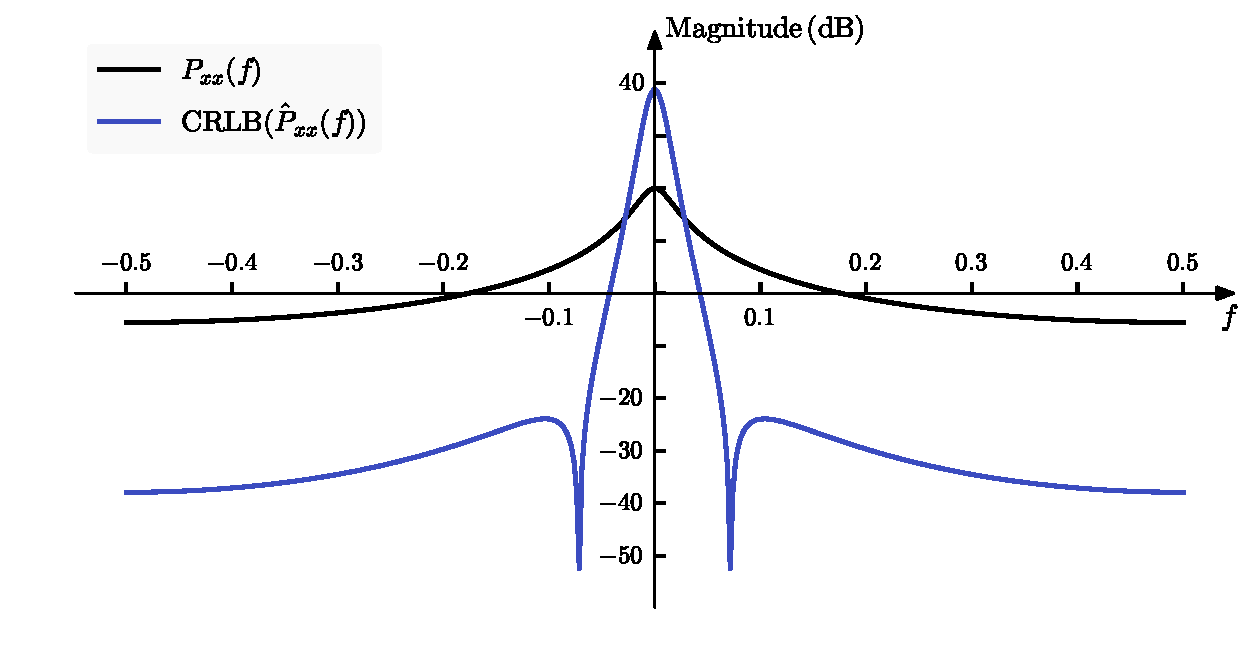
\includegraphics[width=0.9\textwidth]{figuras/problem_3_20.pdf}
\caption{\label{fig:problem_3_20} \(P_{xx}(f)\) y CRLB\((\hat{P}_{xx}(f))\). La CRLB\((\hat{P}_{xx}(f))\) es mas alta cerca de continua debido a la gran sensibilidad de \(P_{xx}(f)\) ante pequeñas variaciones de \(a[1]\) en torno a las bajas frecuencias.}
\end{center}
\end{figure}
Debido a la gran sensibilidad de la PSD ante variaciones de \(a[1]\) en torno a frecuencias cercanas a cero, la CRLB es alta en continua. Por ejemplo, en \(f=0\) se cumple que
\[
  \var\left(\hat{P}_{xx}(0)\right)\geq\frac{4\sigma_u^4(1-a^2[1])\left(a[1]+1\right)^2}{N\left(1+a[1]\right)^8}
  =\frac{4\sigma_u^4(1-a[1])\left(1+a[1]\right)^3}{N\left(1+a[1]\right)^8}
  =\frac{4\sigma_u^4(1-a[1])}{N\left(1+a[1]\right)^5}=7600.
\]


\chapter{Modelos lineales}\label{ch:lineal_models}

\section{Introducción}

En muchos problemas en procesamiento de señales, determinar el estimador MVU es difícil y no siempre puede hacerse. Sin embargo hay un modelo de datos que siempre permite determinar el estimador MVU. Este modelo es el modelo lineal de los datos con el parámetro. 
Si es posible expresar los datos como un modelo lineal, el estimador óptimo, que además es eficiente, se obtiene inmediatamente.

\section{Definición y propiedades}\label{sec:linear_model_definition}

En el problema de ajuste de una recta explicado en la sección \ref{sec:line_fitting}, el modelo de los datos es
\[
 x[n]=A+Bn+w[n],\qquad n=0,\dots,\,N-1,
\]
y el objetivo es determinar los estimadores MVU de \(A\) y \(B\). En notación matricial, este modelo puede expresarse como
\begin{equation}\label{eq:linear_model}
 \x=\Hbf\thetabf+\w,
\end{equation}
donde
\begin{align*}
 \x&=[x[0]\,x[1]\dots x[N-1]]^T\\
 \w&=[w[0]\,w[1]\dots w[N-1]]^T\\
 \thetabf&=[A\,B]^T
\end{align*}
y
\[
 \Hbf=
 \begin{bmatrix}
    1 & 0 \\
    1 & 1 \\
    \vdots & \vdots \\
    1 & N-1
 \end{bmatrix}.
\]
La matriz \(\Hbf\), de dimensiones \(N\times2\) en este caso, es conocida y se denomina \emph{matriz de observación}. El vector de ruido tiene PDF \(\w\sim\mathcal{N}(\mathbf{0},\,\sigma^2\I)\). En estas condiciones, el modelo de los datos de la ecuación \ref{eq:linear_model} es referido como \emph{modelo lineal}.

Como se explicó en el capítulo \ref{ch:crlb}, en ocasiones es posible obtener el estimador MVU si se verifica la condición de igualdad en el teorema de CRLB. Como indica la ecuación \ref{eq:crlb_efficiency_condition_vector},  \(\hat{\thetabf}=\g(\x)\) es el estimador MVU eficiente si
\[
 \frac{\partial\ln p(\x;\,\thetabf)}{\partial\thetabf}=\I(\thetabf)(\g(\x)-\thetabf).
\]
Se determinará si esta condición se satisface en el modelo lineal de la ecuación \ref{eq:linear_model}. La PDF de los datos es
\begin{align}\label{eq:linear_model_pdf}
 p(\x,\,\thetabf)&=\frac{1}{(2\pi)^\frac{N}{2}\det^\frac{1}{2}(\sigma^2\I)}\exp\left\{-\frac{1}{2}(\x-\Hbf\thetabf)^T(\sigma^2\I)^{-1}(\x-\Hbf\thetabf)\right\}\nonumber\\
  &=\frac{1}{(2\pi\sigma^2)^\frac{N}{2}}\exp\left\{-\frac{1}{2\sigma^2}(\x-\Hbf\thetabf)^T(\x-\Hbf\thetabf)\right\},
\end{align}
y al tomar logaritmo y derivar respecto al parámetro, se obtiene que
\begin{align*}
 \frac{\partial p(\x,\,\thetabf)}{\partial\thetabf}&=\frac{\partial}{\partial\thetabf}\left[-\frac{N}{2}\ln(2\pi\sigma^2)-\frac{1}{2\sigma^2}(\x-\Hbf\thetabf)^T(\x-\Hbf\thetabf)\right]\\
 &=-\frac{1}{2\sigma^2}\frac{\partial}{\partial\thetabf}\left[(\x^T-\thetabf^T\Hbf^T)(\x-\Hbf\thetabf)\right]\\
 &=-\frac{1}{2\sigma^2}\frac{\partial}{\partial\thetabf}\left[\x^T\x-\x^T\Hbf\thetabf-\thetabf^T\Hbf^T\x+\thetabf^T\Hbf^T\Hbf\thetabf\right]\\
 &=-\frac{1}{2\sigma^2}\frac{\partial}{\partial\thetabf}\left[\x^T\x-2\x^T\Hbf\thetabf+\thetabf^T\Hbf^T\Hbf\thetabf\right].
\end{align*}
Para calcular la derivada, defínase \(\bbf^T=\x^T\Hbf\) y \(\A=\Hbf^T\Hbf\) simétrica, y teniendo en cuenta que se cumple que
\[
 \frac{\partial \mathbf{b}^T\thetabf}{\partial\thetabf}=\mathbf{b},
 \qquad\frac{\partial \thetabf^T\mathbf{A}\thetabf}{\partial\thetabf}=2\mathbf{A}\thetabf,
\]
como se explica en el apéndice \ref{ap:derivatives_respect_vector}, se obtiene que
\[
 \frac{\partial p(\x,\,\thetabf)}{\partial\thetabf}=-\frac{1}{2\sigma^2}\left[-2\Hbf^T\x+2\Hbf^T\Hbf\thetabf\right]
 =\frac{1}{\sigma^2}\left[\Hbf^T\x-\Hbf^T\Hbf\thetabf\right],
\]
y asumiendo que \(\Hbf^T\Hbf\) es invertible, se llega a que
\[
 \frac{\partial p(\x,\,\thetabf)}{\partial\thetabf}=\frac{\Hbf^T\Hbf}{\sigma^2}\left[\left(\Hbf^T\Hbf\right)^{-1}\Hbf^T\x-\thetabf\right],
\]
ecuación que está factorizada en la forma de la ecuación \ref{eq:crlb_efficiency_condition_vector} con
\begin{align}
 \hat{\thetabf}&=\left(\Hbf^T\Hbf\right)^{-1}\Hbf^T\x\label{eq:linear_model_mvu}\\
 \I(\thetabf)&=\frac{\Hbf^T\Hbf}{\sigma^2}.\label{eq:linear_model_fisher}
\end{align}
Se concluye que el estimador de \(\thetabf\) está dado por la ecuación \ref{eq:linear_model_mvu}, y su matriz de covarianza es
\[
 \C_{\hat{\thetabf}}=\I^{-1}(\thetabf)=\sigma^2\left(\Hbf^T\Hbf\right)^{-1}.
\]
Además, el estimador es eficiente y alcanza la CRLB.

Si bien el razonamiento se realizó en base al problema del ajuste de una recta, el resultado es general cuando los datos se pueden modelar de forma lineal, como indica el siguiente teorema.

\section{Teorema: estimador MVU para el modelo lineal}\label{sec:linear_model_extension}

\paragraph{Hipótesis} Los datos observados pueden modelarse como
\[
 \x=\Hbf\thetabf+\w,
\]
donde \(\x\) de dimensiones \(N\times1\) es el \emph{vector de observaciones}, \(\Hbf\) de dimensiones \(N\times p\) es la \emph{matriz de observación}, conocida, con \(N>p\) y rango \(p\), \(\thetabf\) de dimensiones \(p\times 1\) es el \emph{vector de parámetros} a estimar y \(\w\) de dimensiones \(N\times 1\) es el vector de ruido con PDF \(\mathcal{N}(\mathbf{0},\sigma^2\I)\).

\paragraph{Tésis}

El estimador MVU es
\[
 \hat{\thetabf}=\left(\Hbf^T\Hbf\right)^{-1}\Hbf^T\x
\]
y la matriz de covarianza de \(\hat{\thetabf}\) es
\begin{equation}\label{eq:linear_model_mvu_covariance}
 \C_{\hat{\thetabf}}=\sigma^2\left(\Hbf^T\Hbf\right)^{-1}.
\end{equation}
Además, el estimador MVU es eficiente ya que alcanza la CRLB para todo \(\thetabf\).

Para confirmar que el estimador es insesgado, se observa que
\begin{align*}
 \hat{\thetabf} &= \left(\Hbf^T\Hbf\right)^{-1}\Hbf^T\x\\
 &\overset{(a)}= \left(\Hbf^T\Hbf\right)^{-1}\Hbf^T\left(\Hbf\thetabf+\w\right)\\
 &= \thetabf+\left(\Hbf^T\Hbf\right)^{-1}\Hbf^T\w
\end{align*}
donde en \((a)\) se sustituyó el modelo lineal dado por la ecuación \ref{eq:linear_model}, y al tomar esperanza, se tiene que 
\begin{align*}
 E(\hat{\thetabf}) &= E\left(\thetabf+\left(\Hbf^T\Hbf\right)^{-1}\Hbf^T\w\right)\\
&=\thetabf+\left(\Hbf^T\Hbf\right)^{-1}\Hbf^TE(\w)\\
 &\overset{(b)}=\thetabf
\end{align*}
donde en \((b)\) se tuvo en cuenta que el ruido es de media nula, \(E(\w)=\mathbf{0}\).
Además, el estimador queda completamente especificado estadísticamente. Efectivamente, como \(\hat{\thetabf}\) es una transformación lineal del vector gaussiano \(\x\),
\[
 \hat{\thetabf}\sim\mathcal{N}\left(\thetabf,\,\sigma^2\left(\Hbf^T\Hbf\right)^{-1}\right).
\]

\section{Ejemplos}

\subsection{Ajuste de curva}

Una extensión al problema del ajuste de una recta presentado en la sección \ref{sec:line_fitting} es el ajuste de una curva, en el cual el modelo de los datos es
\[
 x[n]=\sum_{k=0}^{p-1}A_kn^k+w[n],\qquad n=0,\,\dots,\,N-1,
\]
donde \(w[n]\) ese WGN de varianza \(\sigma^2\) y se quiere determinar los \(p\) parámetros \(A_k\), \(k=0,\,\dots,\,p-1\). Al igual que en el problema del ajuste de una recta explicado al comienzo de este capítulo, el modelo de los datos es lineal,
\[
 \x=\Hbf\thetabf+\w
\]
donde
\[
 \Hbf=
 \begin{bmatrix}
  0^0 & 0^1 & 0^2 & \dots & 0^{p-1}\\
  1^0 & 1^1 & 1^2 & \dots & 1^{p-1}\\
  2^0 & 2^1 & 2^2 & \dots & 2^{p-1}\\
  \vdots & \vdots & \vdots &  & \vdots\\
  (N-1)^0 & (N-1)^1 & (N-1)^2 & \dots & (N-1)^{p-1}
 \end{bmatrix}
 \qquad\qquad\textrm{y}\qquad\qquad
 \thetabf=
 \begin{bmatrix}
  A_0\\
  A_1\\
  \vdots\\
  A_{p-1}
 \end{bmatrix}.
\]
La matriz \(\Hbf\) tiene dimensiones \(N\times p\) con \(\Hbf_{ij}=(i-1)^{j-1}\). Una matriz con esta estructura se denomina matriz de Vandermonde. El estimador y su matriz de covarianza están dados por las ecuaciones \ref{eq:linear_model_mvu} y \ref{eq:linear_model_mvu_covariance}. La matriz de información de Fisher para este caso se calculó en el problema de la sección \ref{sec:problem_3_13}. A continuación se muestra una simulación por computadora para el caso con \(p=4\) donde los coeficientes a estimar son
\[
 A_0 = 1,\quad A_1 = 0.73,\quad A_2 = -1.6\times10^{-2},\quad A_3 = 1\times10^{-4},
\]
la cantidad de muestras es \(N=100\) y el ruido tiene varianza \(\sigma^2=10\). La varianza de los coeficientes son los elementos de la diagonal de la matriz de covarianza (ecuación \ref{eq:linear_model_mvu_covariance}), y con estos valores es
\[
 \var(\hat{A}_0)\approx1.49,\quad\var(\hat{A}_1)\approx1.15\times10^{-02},
 \quad\var(\hat{A}_2)\approx6.36\times10^{-06},\quad\var(\hat{A}_3)\approx2.80\times10^{-10}
\]
\begin{figure}[!htb]
\begin{center}
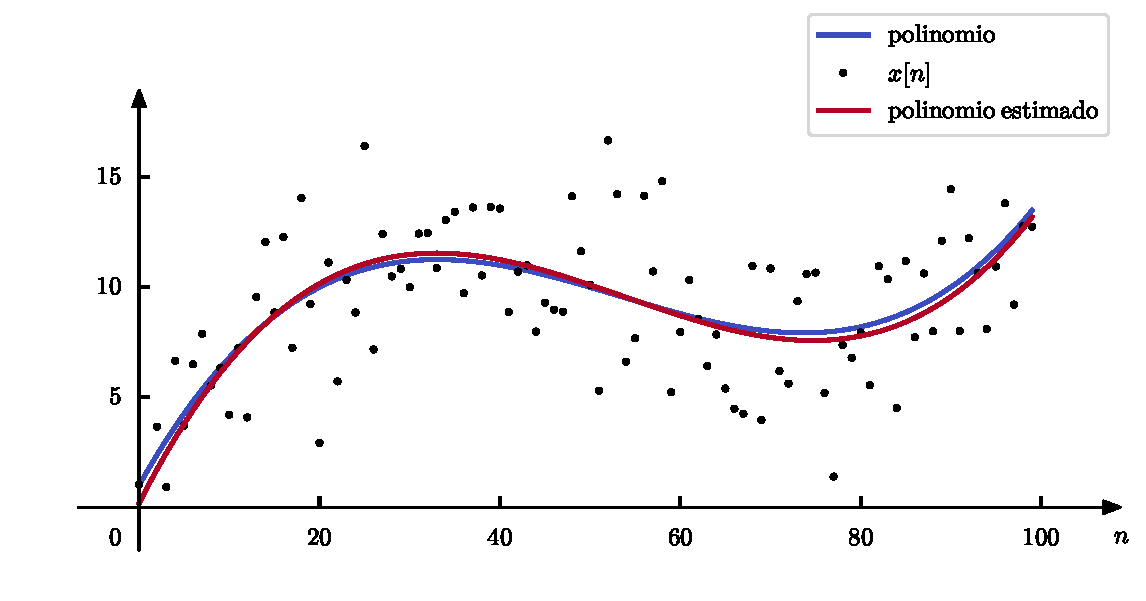
\includegraphics[width=0.95\textwidth]{figuras/example_4_1.pdf}
\caption{\label{fig:example_4_1} Ajuste de curva: estimación de los coeficientes de un polinomio de grado 3 (\(p=4\)). En la figura se muestra el polinomio original, las \(N=100\) muestras ruidosas con potencia de ruido \(\sigma^2=10\) y el polinomio estimado.}
\end{center}
\end{figure}
En la figura \ref{fig:example_4_1} se muestra el resultado de una realización. Las estimaciones de los parámetros en esa realización son
\[
 \hat{A}_0\approx0.188,\quad\hat{A}_1\approx0.808,
 \quad\hat{A}_2\approx-1.77\times10^{-2},\quad\hat{A}_3\approx1.09\times10^{-4}.
\]


\subsection{Análisis de Fourier}\label{sec:linear_model_fourier_analysis}

Muchas señales tienen un comportamiento periódico. La presencia de componentes sinusoidales puede ser detectada mediante el análisis de Fourier, en el cual grandes coeficientes de Fourier indican la presencia de fuertes componentes sinusoidales. Este ejemplo muestra que el análisis de Fourier es en realidad la estimación de los parámetros de un modelo lineal.
Considérese el modelo de datos que consiste en sinusoides en WGN:
\begin{equation}\label{eq:linear_model_fourier_data}
 x[n]=\sum_{k=1}^{M}a_k\cos\left(\frac{2\pi k n}{N}\right)+\sum_{k=1}^{M}b_k\sin\left(\frac{2\pi k n}{N}\right)+w[n],\qquad n=0,\dots,\,N-1, 
\end{equation}
donde \(w[n]\) es WGN. Se asume que las frecuencias de las sinusoides están relacionadas armónicamente, siendo múltiplos de la frecuencia fundamental \(f_1=1/N\), es decir, \(f_k=k/N\). El objetivo es estimar las amplitudes \(a_k\) y \(b_k\) de los cosenos y senos a partir de las observaciones ruidosas \(x[n]\).
Los datos pueden expresarse en el modelo lineal de la ecuación \ref{eq:linear_model} con
\begin{equation}\label{eq:linear_model_fourier_theta}
  \thetabf=\left[a_1\;a_2\dots a_M\;b_1\;b_2\dots b_M\right]^T
\end{equation}
y
\begin{equation}\label{eq:linear_model_fourier_H}
 \Hbf=
 \begin{bmatrix}
    1 & \dots & 1 & 0 & \dots & 0 \\
    \cos\left(\frac{2\pi}{N}\right) & \dots & \cos\left(\frac{2\pi M}{N}\right) & \sin\left(\frac{2\pi}{N}\right)&\dots&\sin\left(\frac{2\pi M}{N}\right)\\
    \vdots & \ddots & \vdots & \vdots & \ddots & \vdots \\
    \cos\left[\frac{2\pi(N-1)}{N}\right] & \dots & \cos\left[\frac{2\pi M (N-1)}{N}\right] & \sin\left[\frac{2\pi(N-1)}{N}\right]&\dots&\sin\left[\frac{2\pi M (N-1)}{N}\right]\\
 \end{bmatrix}. 
\end{equation}
\(\thetabf\) es de dimensión \(2M\times1\) y \(\Hbf\) es de dimensión \(N\times 2M\), donde \(p=2M\). Por lo tanto, para que \(\Hbf\) satisfaga la condición \(N>p\) se requiere que \(M<N/2\).
El cálculo del estimador MVU se simplifica notando que las columnas de \(\Hbf\) son ortogonales. Si se representa \(\Hbf\) en columnas,
\[
 \Hbf=
 \begin{bmatrix}
  \h_1&\h_2&\cdots&\h_{2M}
 \end{bmatrix}
\]
donde \(\h_i\) es la columna \(i\)-ésima de \(\Hbf\), se cumple que
\[
\h_i^T\h_j=0\qquad\qquad\textrm{para }i\neq j.
\]
Considerando esta propiedad,
\[
 \Hbf^T\Hbf = 
 \begin{bmatrix}
  \h_1^T \\
  \h_2^T \\
  \vdots \\
  \h_{2M}^T 
 \end{bmatrix}
 \begin{bmatrix}
  \h_1&\h_2&\cdots&\h_{2M}
 \end{bmatrix}
 = 
 \begin{bmatrix}
  \h_1^T\h_1 & \h_1^T\h_2 & \dots & \h_1^T\h_{2M} \\
  \h_2^T\h_1 & \h_2^T\h_2 & \dots & \h_2^T\h_{2M} \\
  \vdots & \vdots & \ddots & \vdots\\
  \h_{2M}^T\h_1 & \h_{2M}^T\h_2 & \dots & \h_{2M}^T\h_{2M}
 \end{bmatrix}
\]
es una matriz diagonal y por lo tanto, fácil de invertir.
La ortogonalidad de las columnas proviene de las relaciones
\begin{align*}
\sum_{n=0}^{N-1}\cos\left(\frac{2\pi in}{N}\right)\cos\left(\frac{2\pi jn}{N}\right)&=\frac{N}{2}\delta_{ij}\\
\sum_{n=0}^{N-1}\sin\left(\frac{2\pi in}{N}\right)\sin\left(\frac{2\pi jn}{N}\right)&=\frac{N}{2}\delta_{ij}\\
\sum_{n=0}^{N-1}\cos\left(\frac{2\pi in}{N}\right)\sin\left(\frac{2\pi jn}{N}\right)&=0\quad\forall i,\,j,
\end{align*}
válidas para \(i,\,j=1,\dots,M<N/2\), que se demuestran en el problema de la sección \ref{sec:problem_4_5}. A partir de estas relaciones, se obtiene que
\[
    \Hbf^T\Hbf = \left[ \begin{array}{cccc}
    \frac{N}{2} & 0 & \dots & 0 \\
    0 & \frac{N}{2} & \dots & 0 \\
    \vdots & \vdots & \ddots & \vdots\\
    0 & 0 & \dots & \frac{N}{2}
    \end{array} 
    \right]
    =\frac{N}{2}\mathbf{I},
\]
por lo que el estimador MVU de las amplitudes es
\begin{align*}
    \boldsymbol{\hat{\thetabf}} &= \left(\Hbf^T\Hbf\right)^{-1}\Hbf^T\x
    =\frac{2}{N}\mathbf{I}\Hbf^T\x=\frac{2}{N}
    \left[ \begin{array}{c}
    \h_1^T \\
    \h_2^T \\
    \vdots  \\
    \h_{2M}^T \end{array} 
    \right]\x
    =\left[ \begin{array}{c}
    \frac{2}{N}\h_1^T\x \\
    \frac{2}{N}\h_2^T\x \\
    \vdots  \\
    \frac{2}{N}\h_{2M}^T\x \end{array}
    \right].
\end{align*}
Finalmente
\begin{equation}\label{eq:linear_model_fourier_mvu}
 \begin{aligned}
  \hat{a}_k &= \frac{2}{N}\sum_{n=0}^{N-1}x[n]\cos\left(\frac{2\pi kn}{N}\right)\\
  \hat{b}_k &= \frac{2}{N}\sum_{n=0}^{N-1}x[n]\sin\left(\frac{2\pi kn}{N}\right).
\end{aligned}
\end{equation}
Se concluye que \(\hat{a}_k\) y \(\hat{b}_k\) son los coeficientes de Fourier de \(x[n]\), como se muestra en el apéndice \ref{ap:rdft} (ver la ecuación \ref{eq:rdft}).
La matriz de covarianza es
\begin{equation}\label{eq:linear_model_fourier_mvu_covariance}
 \mathbf{C}_{\hat{\theta}}=\sigma^2\left(\Hbf^T\Hbf\right)^{-1}=\frac{2\sigma^2}{N}\mathbf{I}. 
\end{equation}
Como la matriz de covarianza es diagonal, los estimadores son independientes.

\subsection{Identificación de un sistema}\label{sec:linear_model_system_identification_example}

En ocasiones es de interés identificar un sistema desconocido. Un modelo común del sistema es como un filtro de respuesta al impulso finita (FIR, \emph{finte impulse response}), como se muestra en la figura \ref{fig:identificacion_modelo_fir}, y el objetivo es estimar los coeficientes \(h[k]\) del filtro. La estrategia es alimentar al sistema con una entrada \(u[n]\) conocida y observar la salida, que idealmente será \(\sum_{k=0}^{p-1}h[k]u[n-k]\), y a partir de ésta, estimar los coeficientes  del filtro, o equivalentemente, la respuesta al impulso.
\begin{figure}[!htb]
  \begin{minipage}[c]{0.50\textwidth}
    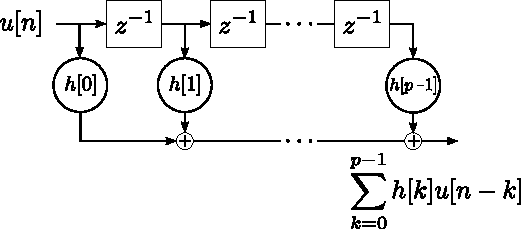
\includegraphics[width=\textwidth]{figuras/identificacion_modelo_fir.pdf}
  \end{minipage}\hfill
  \begin{minipage}[c]{0.40\textwidth}
    \caption{
       Modelo de un sistema desconocido como filtro FIR.
    } \label{fig:identificacion_modelo_fir}
  \end{minipage}
\end{figure}
En la práctica, la salida observada es ruidosa, por lo que un modelo mas apropiado es como en la figura \ref{fig:identificacion_esquema}.
\begin{figure}[!htb]
  \begin{minipage}[c]{0.50\textwidth}
    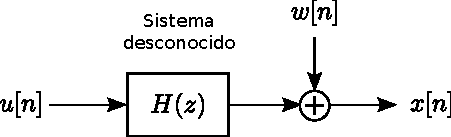
\includegraphics[width=0.9\textwidth]{figuras/identificacion_esquema.pdf}
  \end{minipage}\hfill
  \begin{minipage}[c]{0.40\textwidth}
    \caption{
       Modelo del sistema con la salida corrompida con ruido.
    } \label{fig:identificacion_esquema}
  \end{minipage}
\end{figure}
Supóngase que la entrada es provista en \(n=0,\dots,\,N-1\) y la salida se observa en el mismo intervalo,
\[
 x[n]=\sum_{k=0}^{p-1}h[k]u[n-k]+w[n]\qquad n = 0,\dots,\,N-1,
\]
donde se asume que \(u[n]=0\) si \(n<0\). En notación matricial, las ecuaciones se pueden expresar como
\begin{equation*}
\x=
\underbrace{
\begin{bmatrix}
u[0]  & 0     &   \cdots & 0\\
u[1]  & u[0]  &   \cdots & 0\\
\vdots & \vdots & \ddots  & \vdots\\
u[p-1] & u[p-2] &  \cdots & u[0]\\
\vdots & \vdots &  & \vdots\\
u[N-1] & u[N-2] &  \cdots & u[N-p]
\end{bmatrix}}_{\displaystyle\Hbf}
\underbrace{
\begin{bmatrix}
h[0]\\
h[1]\\
\vdots\\
h[p-1]
\end{bmatrix}}_{\displaystyle\thetabf} + 
\w.
\end{equation*}
Asumiendo que el ruido \(w[n]\) es WGN, las ecuaciones tienen la forma del modelo lineal de la ecuación \ref{eq:linear_model}, por lo que el estimador MVU de la respuesta al impulso es
\[
 \hat{\thetabf} = \left(\Hbf^T\Hbf\right)^{-1}\Hbf^T\x,
\]
y la matriz de covarianza del estimador es 
\[
 \C_{\hat{\thetabf}} = \sigma^2\left(\Hbf^T\Hbf\right)^{-1}.
\]
Se comenzará calculando \(\Hbf^T\Hbf\). Para hacerlo, se parte notando que la columna \(j\)-ésima de \(\Hbf\) es
\[
  [\Hbf]_j = [\underbrace{0\,\dots 0}_{j-1}\,u[0]\dots u[N-j]]^T,\qquad 1\leq j \leq p,
\]
por lo que el elemento \((i,\,j)\) de \(\Hbf^T\Hbf\), con \(i\geq j\), es
\begin{align*}
 [\Hbf^T\Hbf]_{ij}=[\Hbf]_i^T[\Hbf]_j&=[\underbrace{0\,\dots 0}_{i-1}\,u[0]\dots u[N-i]]
 \begin{bmatrix}
  0 \\ \vdots\\ 0\\ u[0]\\ \vdots\\ u[N-j]
 \end{bmatrix}
 \setlength{\arraycolsep}{0pt} % Avoid any column space in arrays that follow
  \begin{array}{ c }
    \left.\kern-\nulldelimiterspace
    \vphantom{\begin{array}{ c }
        0 \\ % Second row
      \vdots \\ % Third row
    \end{array}}
    \right\}\text{$j-1$}
    \vphantom{u[0]}\\
    \vphantom{\vdots}\\
    \vphantom{u[N-j]}\\
    \vphantom{u[N-j]}
  \end{array}\\
   &=\underbrace{0+\dots+0}_{i-1}+u[0]u[i-j]+u[1]u[i-j+1]+\dots+u[N-i]u[N-j]\\
   &=\sum_{n=0}^{N-i}u[n]u[n+i-j].
\end{align*}
Para valores arbitrarios de \((i,\,j)\), esto se generaliza como
\begin{equation}\label{eq:sample_autocorrelation_tmp}
 [\Hbf^T\Hbf]_{ij}=\sum_{n=0}^{N-\max(i,\,j)}u[n]u[n+|i-j|].
\end{equation}
Notar que la matriz \(\Hbf^T\Hbf\) es simétrica. 
Como se muestra en el problema de la sección \ref{sec:problem_4_7}, en el caso en que \(N\gg p\) se cumple que
\begin{equation}\label{eq:sample_autocorrelation_1}
 [\Hbf^T\Hbf]_{ij}\approx\sum_{n=0}^{N-1-|i-j|}u[n]u[n+|i-j|],
\end{equation}
que es la \emph{función de correlación} de la secuencia determinística \(u[n]\). De esta forma,
\begin{equation}\label{eq:system_identification_correlation_matrix}
\Hbf^T\Hbf=N\begin{bmatrix}
r_{uu}[0] & r_{uu}[1] & r_{uu}[2] & \cdots & r_{uu}[p-1]\\
r_{uu}[1] & r_{uu}[0] & r_{uu}[1] & \cdots & r_{uu}[p-2]\\
r_{uu}[2] & r_{uu}[1] & r_{uu}[0] & \cdots & r_{uu}[p-3]\\
\vdots & \vdots & \vdots & \ddots & \vdots\\
r_{uu}[p-1] & r_{uu}[p-2] & r_{uu}[p-3] &  \cdots & r_{uu}[0]\\
\end{bmatrix}
=N\mathbf{R}_{uu}
\end{equation}
donde
\begin{equation}\label{eq:sample_autocorrelation_u}
 r_{uu}[k]=\frac{1}{N}\sum_{n=0}^{N-1-k}u[n]u[n+k]
\end{equation}
es la función de autocorrelación muestral de \(u[n]\).
El motivo de realizar la aproximación es que de esta forma, la matriz \(\Hbf^T\Hbf\) además de ser simétrica, es una matriz Toeplitz de autocorrelación, lo que simplifica los resultados. Esto es
\[
 \left[\Hbf^T\Hbf\right]_{ij}=\left[\Hbf^T\Hbf\right]_{ji}\quad\textrm{(simétrica)}\qquad\qquad
 \left[\Hbf^T\Hbf\right]_{ij}=\left[\Hbf^T\Hbf\right]_{i+k,j+k}\quad\textrm{(Toeplitz)}.
\]
Por otro lado, 
\[
 \Hbf^T\x=
\begin{bmatrix}
u[0]  & u[1] & \cdots & u[p-1] & \cdots & u[N-1]\\
 0    & u[0] & \cdots & u[p-2] & \cdots & u[N-2]\\
\vdots & \vdots & \ddots  & \vdots & & \vdots\\
0    & 0   &  \cdots & u[0] & \cdots & u[N-p]\\
\end{bmatrix}
\begin{bmatrix}
x[0]\\
x[1]\\
\vdots\\
x[N-1]
\end{bmatrix}
\]
por lo que el elemento \(i+1\) de \(\Hbf^T\x\), \(i=0,\dots,\,p-1\) es
\begin{align*}
\left[\Hbf^T\x\right]_{i+1}&=\sum_{n=0}^{N-i}u[n]x[n+i]\\
&=Nr_{ux}[i],
\end{align*}
donde
\begin{equation}\label{eq:sample_crosscorrelation_ux}
r_{ux}[k]=\frac{1}{N}\sum_{n=0}^{N-k}u[n]x[n+k] 
\end{equation}
es la correlación cruzada muestral entre \(u[n]\) y \(x[n]\). Finalmente, \(\Hbf^T\x\) queda
\begin{equation}\label{eq:system_identification_crosscorrelation}
 \Hbf^T\x=N\left[ \begin{array}{c}
 r_{ux}[0] \\
 r_{ux}[1] \\
 \vdots \\
 r_{ux}[p-1] \\
\end{array} \right] = N\mathbf{r}_{ux},
\end{equation}
donde \(\mathbf{r}_{ux}\) es vector de correlación cruzada entre \(u[n]\) y \(x[n]\).
Sustituyendo las ecuaciones \ref{eq:system_identification_correlation_matrix} y \ref{eq:system_identification_crosscorrelation} en las ecuaciones \ref{eq:linear_model_mvu} y \ref{eq:linear_model_mvu_covariance} del estimador óptimo y la matriz de covarianza del modelo lineal se llega a que
\begin{align}
  \mathbf{\hat{h}} &= \mathbf{R}_{uu}^{-1}\mathbf{r}_{ux}\label{eq:system_identification_h_opt}\\
   \C_{\hat{h}} &= \frac{\sigma^2}{N}\mathbf{R}_{uu}^{-1}.\label{eq:system_identification_h_covariance}
\end{align}
Los coeficientes de varianza mínima del filtro se obtienen multiplicando la matriz de autocorrelación inversa de la entrada con la correlación cruzada entre la entrada y la salida. Este resultado coincide con los coeficientes del filtro de Wiener, y en ese contexto, el sistema de ecuaciones \ref{eq:system_identification_h_opt} se denomina \emph{ecuaciones de Wiener–Hopf} (ver por ejemplo el capítulo 7 de \cite{hayes96statistical}).

La ecuación \ref{eq:system_identification_h_covariance} indica que la varianza de los coeficientes óptimos \(\mathbf{\hat{h}}\) dependen de la señal de prueba \(u[n]\) a través de  \(\mathbf{R}_{uu}\). Es de interés encontrar la señal de prueba que produzca la mínima varianza de los coeficientes. Se mostrará a continuación que la señal de prueba que minimiza la varianza es ruido no correlacionado.
La varianza del coeficiente \(i\)-ésimo \(\hat{h}[i]\) es
\[
 \var(\hat{h}[i])=[\C_{\hat{h}}]_{ii}=\mathbf{e}_i^T\C_{\hat{h}}\mathbf{e}_i
 \qquad \textrm{con}\qquad \mathbf{e}_i=[0\,0\dots 0\,\underbrace{1}_{\textrm{posición }i}\,0\dots 0\,0]^T.
\]
Como \(\C_{\hat{h}}\) es simétrica y definida positiva, también lo es \(\C_{\hat{h}}^{-1}\), por lo que puede factorizarse aplicando la descomposición de Cholesky\footnote{Ver por ejemplo \url{https://en.wikipedia.org/wiki/Cholesky_decomposition}.} como
\[
 \C_{\hat{h}}^{-1} = \mathbf{D}^T\mathbf{D},
\]
donde \(\D\) es una matriz \(p\times p\) invertible\footnote{Una matriz de covarianza es semidefinida-positiva. A una matriz simétrica y semi-definida positiva también puede aplicarse la descomposición de Cholesky si se permite que elementos de la diagonal de \(\D\) sean nulos, lo que hace que \(\D\) no sea invertible. Es por esto que se asume aquí que \(\C_{\hat{h}}\) es definida positiva.}.
Teniendo esto en cuenta y notando que
\[
\mathbf{e}_i^T\mathbf{I}\mathbf{e}_i=1
\qquad\Rightarrow\qquad\mathbf{e}_i^T\mathbf{D}^{T}{\mathbf{D}^{T}}^{-1}\mathbf{e}_i=1
\qquad\Rightarrow\qquad(\mathbf{e}_i^T\mathbf{D}^{T}{\mathbf{D}^{T}}^{-1}\mathbf{e}_i)^2=1,
\]
se definen los vectores
\[
\boldsymbol{\xi}_1=\mathbf{D}\mathbf{e}_i,\qquad\qquad
\boldsymbol{\xi}_2={\mathbf{D}^{T}}^{-1}\mathbf{e}_i,
\]
y la igualdad se puede expresar como
\[
 \left(\boldsymbol{\xi}^T_1\boldsymbol{\xi}_2\right)^2=1.
\]
Aplicando la desigualdad de Cauchy-Schwarz (ecuación \ref{eq:cauchy_schwarz_inequality}), se tiene que
\[
 \left(\boldsymbol{\xi}^T_1\boldsymbol{\xi}_1\right)\left(\boldsymbol{\xi}^T_2\boldsymbol{\xi}_2\right) \geq \left(\boldsymbol{\xi}^T_1\boldsymbol{\xi}_2\right)^2=1,
\]
y sustituyendo, se llega a que
\begin{align*}
    (\boldsymbol{\xi}_1^T\boldsymbol{\xi}_1)(\boldsymbol{\xi}_2^T\boldsymbol{\xi}_2) &= (\mathbf{e}_i^T\mathbf{D}^{T}\mathbf{D}\mathbf{e}_i)(\mathbf{e}_i^T{{\mathbf{D}^{T}}^{-1}}^T{\mathbf{D}^{T}}^{-1}\mathbf{e}_i)\\
    &= (\mathbf{e}_i^T\mathbf{D}^{T}\mathbf{D}\mathbf{e}_i)(\mathbf{e}_i^T\mathbf{D}^{-1}{\mathbf{D}^{T}}^{-1}\mathbf{e}_i)\\
    &= (\mathbf{e}_i^T\C_{\hat{h}}^{-1}\mathbf{e}_i)(\mathbf{e}_i^T\C_{\hat{h}}\mathbf{e}_i)\\
    &\geq 1.
\end{align*}
Finalmente, se obtiene que
\begin{align*}
    \mathbf{e}_i^T\C_{\hat{h}}\mathbf{e}_i=\var(h[i])\geq\frac{1}{\mathbf{e}_i^T\C_{\hat{h}}^{-1}\mathbf{e}_i}.
\end{align*}
Se observa que la varianza es mínima cuando la desigualdad de Cauchy-Schwarz se  cumple con igualdad. Esto sucede cuando \(\boldsymbol{\xi}_1\) y \(\boldsymbol{\xi}_2\) son colineales, es decir
\[
 \boldsymbol{\xi}_1=c\boldsymbol{\xi}_2,
\]
donde \(c\) es una constante. Por lo tanto, la condición para que la varianza de todos los coeficientes sea mínima es que
\[
 \mathbf{D}\mathbf{e}_i=c_i{\mathbf{D}^{T}}^{-1}\mathbf{e}_i,
\]
o equivalentemente,
\[
  \mathbf{D}^T\mathbf{D}\mathbf{e}_i=c_i\mathbf{e}_i,\qquad\qquad i=1,\,2\dots,p,
\]
donde \(c_i\) son constantes, \(i=1,\dots,\,p\). Teniendo en cuenta que \( \mathbf{D}^T\mathbf{D}=\C_{\hat{h}}^{-1}\), la condición queda
\[
 \C_{\hat{h}}^{-1}\mathbf{e}_i=c_i\mathbf{e}_i,\qquad\qquad i=1,\,2\dots,p, 
\]
o en palabras, la columna \(i\)-ésima de \(\C_{\hat{h}}^{-1}\) tiene solo un elemento no nulo \(c_i\) en la posición \(i\).
Se concluye que la matriz de covarianza inversa \(\C_{\hat{h}}^{-1}\) tiene que ser diagonal. Por la ecuación \ref{eq:system_identification_h_covariance}
\[
  \C_{\hat{h}}^{-1} = \frac{N}{\sigma^2}\mathbf{R}_{uu},
\]
indicando que la matriz de autocorrelación de la entrada debe ser diagonal,
\[
 r_{uu}[k]=0\qquad \forall k\neq0,
\]
es decir,
\[
 \mathbf{R}_{uu}=r_{uu}[0]\I,
\]
lo cual se cumple si \(u[n]\) es ruido no correlacionado.
En esas condiciones, el estimador queda (ecuación \ref{eq:system_identification_h_opt})
\[
 \mathbf{\hat{h}} = \mathbf{R}_{uu}^{-1}\mathbf{r}_{ux}=\frac{1}{r_{uu}[0]}\mathbf{r}_{ux},
\]
resultando en
\begin{equation}\label{eq:system_identification_h_opt_wn}
 \hat{h}[i]=\frac{r_{ux}[i]}{r_{uu}[0]},\qquad i=1,\,2\dots,p.
\end{equation}
Además, de la ecuación \ref{eq:system_identification_h_covariance} se obtiene que la matriz de covarianza es
\[
 \C_{\hat{h}} = \frac{\sigma^2}{Nr_{uu}[0]}\I
\]
de lo cual se deduce que por se una matriz diagonal, los coeficientes son independientes con varianza
\[
\var(\hat{h}[i]) = \frac{\sigma^2}{Nr_{uu}[0]}, \qquad i=1,\,2\dots,p.
\]
Por una deducción en el dominio de la frecuencia del problema de identificación de un sistema, ver el problema de la sección \ref{sec:problem_4_8}.

\subsubsection{Simulación por computadora}

A continuación se muestran los resultados de una simulación por computadora de la estimación de un sistema. El sistema desconocido es un filtro de respuesta al impulso finita (\emph{finite impulse response}, FIR) de orden \(p=11\) causal de respuesta al impulso triangular, la cual se muestra en la figura \ref{fig:system_identification_impulse_response}.
\begin{figure}[!htb]
  \begin{minipage}[c]{0.65\textwidth}
    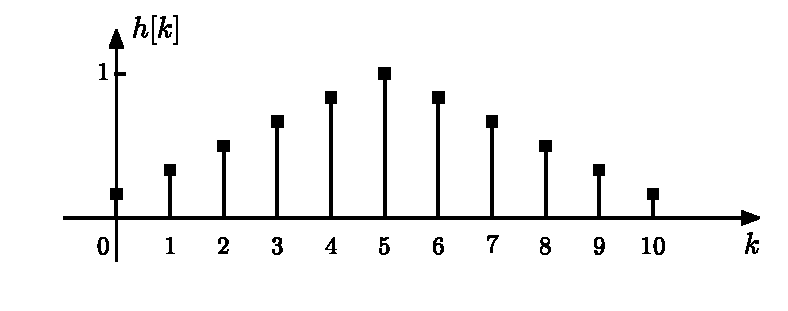
\includegraphics[width=1\textwidth]{figuras/system_identification_impulse_response.pdf}
  \end{minipage}\hfill
  \begin{minipage}[c]{0.25\textwidth}
    \caption{
       Respuesta al impulso del filtro a estimar.
    } \label{fig:system_identification_impulse_response}
  \end{minipage}
\end{figure}
Se usan dos tipos de señales de prueba de largo \(N=1000\) muestras. La señal \(u_1[n]\) es ruido blanco gaussiano y la señal \(u_2[n]\) es ruido coloreado. Ambas señales tienen potencia unidad. 

\paragraph{Ruido coloreado \(u_2[n]\)} El ruido coloreado \(u_2[n]\) usado como señal de prueba es un proceso AR(2),
\[
 u_2[n]+a_1u_2[n-1]+a_2u_2[n-2]=v[n],
\]
con \(a_1=-0.8\) y \(a_2=0.64\), donde \(v[n]\) es ruido blanco gaussiano. Hay que tener en cuenta que la relación de potencias entre \(v[n]\) y \(u_2[n]\) es (ver el capítulo 1 de \cite{haykin2014adaptive})
\[
 \sigma_{u_2}^2=\frac{1+a_2}{(1-a_2)\left[(1+a_2)^2-a_1^2\right]}\sigma_v^2,
\]
por lo que \(v[n]\) debe tener la potencia adecuada para que \(u_2[n]\) tenga potencia unidad. La PSD \(S_{u_2u_2}(\omega)\) del proceso \(u_2[n]\) es
\[
 S_{u_2u_2}(\omega)=\frac{\sigma_v^2}{\left|1+a_1e^{-j\omega}+a_2e^{-2j\omega}\right|^2},
\]
y la función de autocorrelación puede obtenerse mediante la transformada inversa de Fourier de la PSD (calculada por computadora) o mediante las ecuaciones de Yule-Walker. Con los parámetros elegidos, la señal \(u_2[n]\) tiene PSD y función de autocorrelación mostradas en la figura \ref{fig:system_identification_u2_input}.
\begin{figure}[!htb]
  \begin{minipage}[c]{0.65\textwidth}
    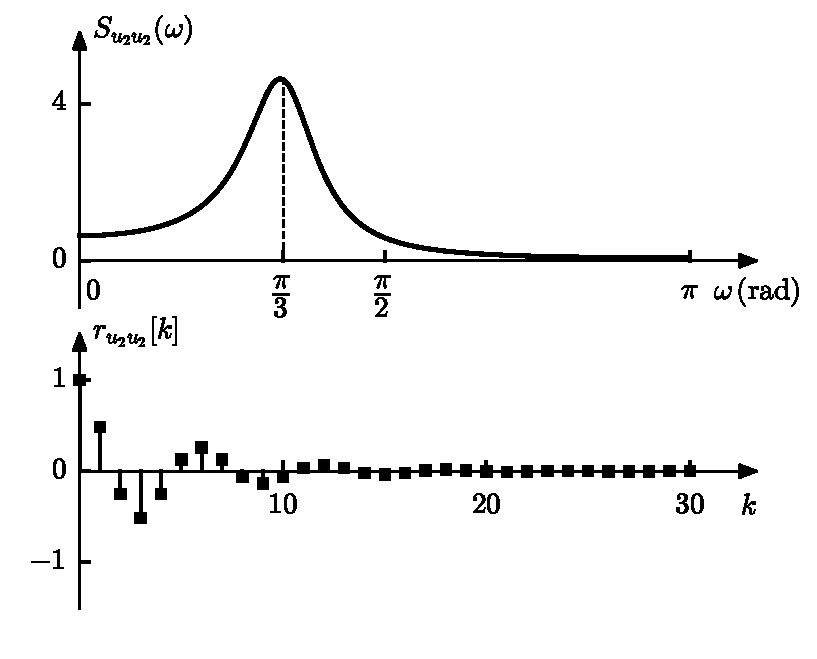
\includegraphics[width=1\textwidth]{figuras/system_identification_u2_input_v2.pdf}
  \end{minipage}\hfill
  \begin{minipage}[c]{0.25\textwidth}
    \caption{
       PSD \(S_{u_2u_2}(\omega)\) y función de autocorrelación \(r_{u_2u_2}[k]\) de la señal \(u_2[n]\). El proceso es pasabanda con frecuencia de resonancia de \(\pi/3\) radianes.
    } \label{fig:system_identification_u2_input}
  \end{minipage}
\end{figure}

\paragraph{Salidas del sistema desconocido} Los procesos \(u_1[n]\) y \(u_2[n]\) se emplean como entradas al sistema desconocido, produciendo la salidas \(x_1[n]\) y \(x_2[n]\) respectivamente, las cuales se observan contaminadas con ruido (WGN) \(w[n]\). La SNR de las señales observadas es 0 dB, es decir, la potencia \(\sigma^2_w\) del ruido  es igual a la potencia \(\sigma^2_{x_i}\) de las salidas \(x_i[n]\), \(i=1,\,2\). La potencia de las salidas es
\begin{align*}
 \sigma_{x_i}^2 & \overset{(a)}{=}E\left(x_i^2[n]\right)\\
   &=E\left[\left(\sum_{k=0}^{p-1}h[k]u_i[n-k]\right)^2\right]\\
   &=E\left[\left(\sum_{k=0}^{p-1}h[k]u_i[n-k]\right)\left(\sum_{l=0}^{p-1}h[l]u_i[n-l]\right)\right]\\
   &=E\left(\sum_{k=0}^{p-1}\sum_{l=0}^{p-1}h[k]h[l]u_i[n-k]u_i[n-l]\right)\\
   &=\sum_{k=0}^{p-1}\sum_{l=0}^{p-1}h[k]h[l]E\left(u_i[n-k]u_i[n-l]\right)\\
   &\overset{(b)}{=}\sum_{k=0}^{p-1}\sum_{l=0}^{p-1}h[k]h[l]\sigma_{u_i}^2\delta_{kl}\\
   &=\sigma_{u_i}^2\sum_{k=0}^{p-1}h^2[k],
\end{align*}
donde en \((a)\) se consideró que \(E(x_i[n])=0\) y en \((b)\) se tuvo en cuenta que \(E(u_i[n-k]u_i[n-l])=\sigma_{u_i}^2\) si \(k=l\) y cero en otro caso.
\begin{figure}[!htb]
\begin{center}
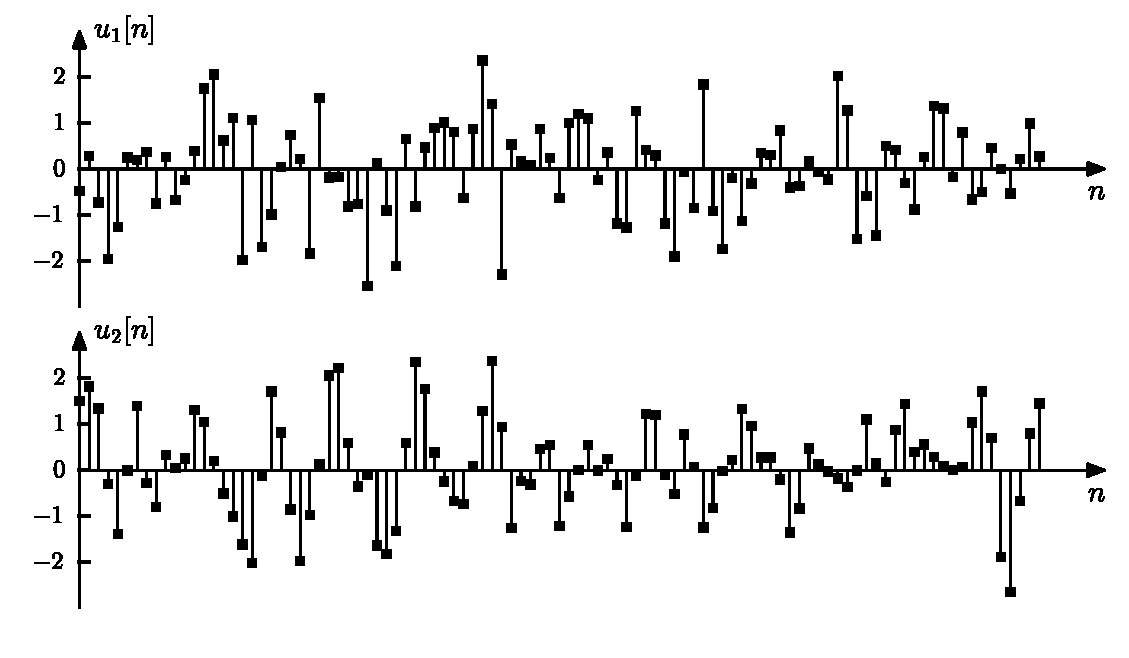
\includegraphics[width=0.9\textwidth]{figuras/system_identification_inputs_v2.pdf}
\caption{\label{fig:system_identification_inputs} Primeras 100 muestras de una realización de los procesos \(u_1[n]\) y \(u_2[n]\) de entrada. \(u_1[n]\) es WGN y \(u_2[n]\) es un proceso AR(2). Se observa la naturaleza pseudo-periódica de \(u_2[n]\), acorde a su PSD.}
\end{center}
\end{figure}
En la figura \ref{fig:system_identification_inputs} se muestran las primeras 10 muestras de una realización de los procesos de entrada \(u_1[n]\) y \(u_2[n]\) y en la figura \ref{fig:system_identification_outputs} se muestran las primeras 100 muestras de las salidas \(x_1[n]\) y \(x_2[n]\) y las salidas observadas contaminadas con ruido \(x_1[n]+w[n]\) y \(x_2[n]+w[n]\).
\begin{figure}[!htb]
\begin{center}
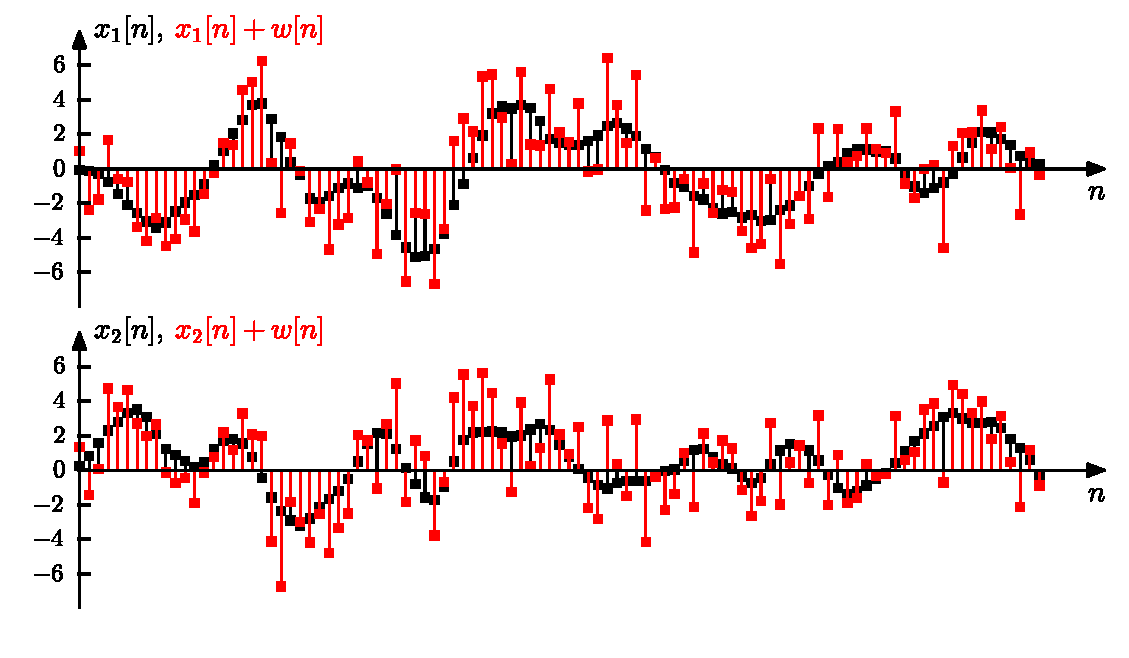
\includegraphics[width=0.9\textwidth]{figuras/system_identification_outputs_v2.pdf}
\caption{\label{fig:system_identification_outputs} Primeras 100 muestras de una realización de las salidas \(x_1[n]\) y \(x_2[n]\) del sistema desconocido. \(u_1[n]\) es WGN y \(u_2[n]\) es un proceso AR(2). Se observa la naturaleza pseudo-periódica de \(u_2[n]\), acorde a su PSD.}
\end{center}
\end{figure}

\paragraph{Identificación del sistema} Se asume que se conoce el orden \(p\) del filtro FIR desconocido. En el caso en que el proceso de entrada es WGN, como \(u_1[n]\), esto no implica un pérdida de generalidad, ya que los estimadores de cada coeficiente son independientes y de igual varianza, y por lo tanto, se puede usar un valor grande de \(p\) sin cambiar los resultados. En este caso, la estimación de los coeficientes que superen el orden del sistema desconocido, tendrán un valor cercano a cero. 

Para identificar el sistema, se calculan las primeras \(p\) muestras de la autocorrelación muestral de la entrada \(u_i[n]\) y la correlación cruzada muestral entre la entrada \(u_i[n]\) y la salida contaminada con ruido \(x_i[n]+w[n]\) empleando las ecuaciones \ref{eq:sample_autocorrelation_u} y \ref{eq:sample_crosscorrelation_ux} respectivamente. Con la autocorrelación se construye la matriz Toeplitz de autocorrelación de tamaño \(p\), y se obtiene el estimador del sistema resolviendo el sistema de ecuaciones \ref{eq:system_identification_h_opt}. El resultado de la estimación para una realización de cada tipo de entrada se muestra en la figura \ref{fig:system_identification_impulse_response_mvu}.
\begin{figure}[!htb]
  \begin{minipage}[c]{0.65\textwidth}
    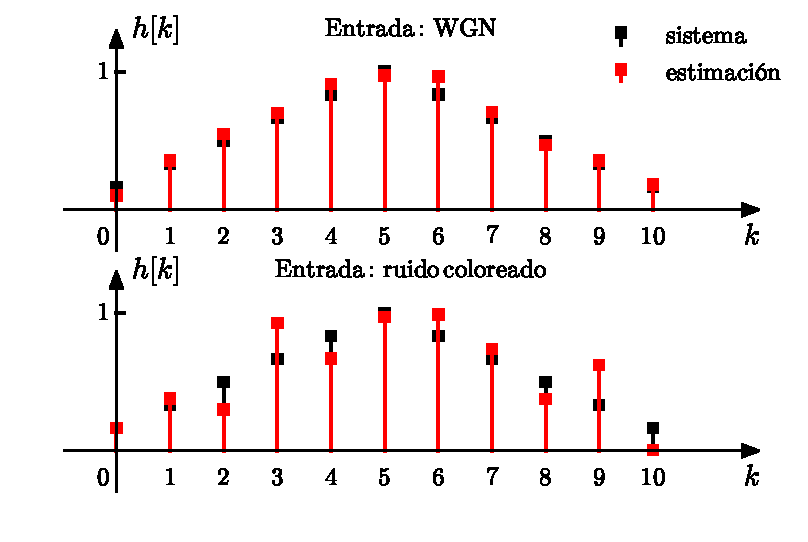
\includegraphics[width=1\textwidth]{figuras/system_identification_impulse_response_mvu_v2.pdf}
  \end{minipage}\hfill
  \begin{minipage}[c]{0.25\textwidth}
    \caption{
       Resultado de la estimación de los coeficientes \(h[k]\) del sistema desconocido empleando ruido blanco y ruido coloreado como señales de prueba. 
    } \label{fig:system_identification_impulse_response_mvu}
  \end{minipage}
\end{figure}
Como se observa en la figura, el error en la estimación es considerablemente grande debido a que si bien el número de muestras \(N=1000\) de las señales de prueba es grande, la relación señal a ruido es mala. En el caso particular de las realizaciones mostradas en las figuras, la estimación usando WGN parece un poco mejor que la estimación empleando ruido coloreado. Esto es acorde a lo concluido previamente de que la entrada que produce estimadores de mínima varianza es WGN.

Finalmente, se calcula la CRLB de los estimadores. Para hacerlo, se calcula la matriz de covarianza empleando la ecuación \ref{eq:system_identification_h_covariance}, y los elementos de la diagonal de la matriz son la varianza de cada coeficiente. También se calcula la varianza práctica de los estimadores de cada coeficiente. Para esto, se repite el experimento y se calcula el error cuadrático (\emph{square error}, SE) de cada coeficiente en cada experimento como
\[
 \operatorname{SE}(\hat{h}[i])=(\hat{h}[i]-h[i])^2.
\]
Promediando el error cuadrático en todos los experimentos, se obtiene la varianza o el error cuadrático medio. En la figura \ref{fig:system_identification_crlb_mse} se muestra la CRLB y la varianza práctica repitiendo el experimento 10000 veces.
\begin{figure}[!htb]
  \begin{minipage}[c]{0.65\textwidth}
    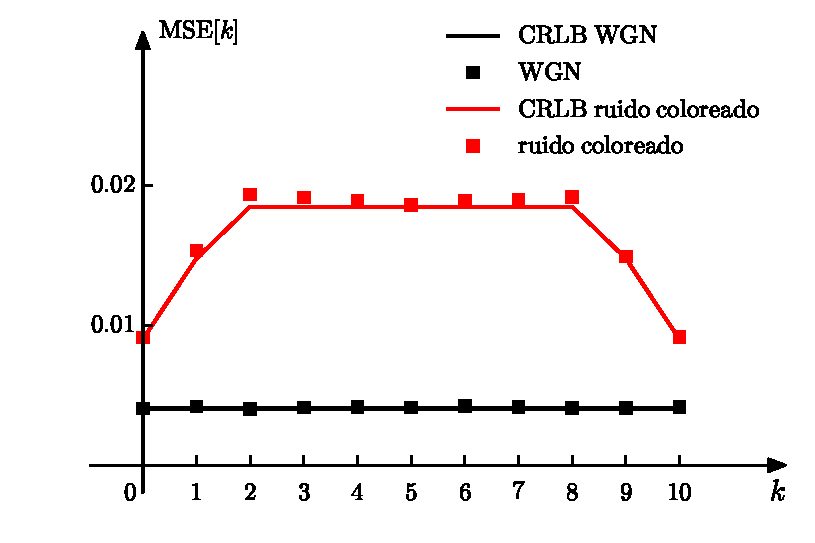
\includegraphics[width=1\textwidth]{figuras/system_identification_crlb_mse_v2.pdf}
  \end{minipage}\hfill
  \begin{minipage}[c]{0.25\textwidth}
    \caption{
       Comparación de la CRLB y la varianza práctica de los estimadores de cada coeficiente del sistema desconocido. En este problema, los estimadores son eficientes. Además, la entrada que produce estimadores de varianza mínima es WGN.
    } \label{fig:system_identification_crlb_mse}
  \end{minipage}
\end{figure}
Como se observa en la figura y se dedujo analíticamente, los estimadores son eficientes en el sentido de que alcanzan la CRLB. Adicionalmente, también se observa que la estimación empleando WGN produce estimadores de varianza menor que la producida empleando ruido coloreado.

\section{Extensión del modelo lineal}\label{sec:linear_model_coloured_noise_extension}

Una formulación mas general del modelo lineal admite ruido que no es blanco. El \emph{modelo lineal general} asume que el ruido es
\[
  \w\sim\mathcal{N}(\mathbf{0},\C),
\]
donde \(\C\) es una matriz genérica de covarianza y no una matriz identidad escalada. La determinación del estimador MVU puede hacerse de forma análoga al caso con ruido blanco (ver el problema de la sección \ref{sec:problem_4_9}). A continuación se realizará la deducción empleando un enfoque de blanqueado. Asumiendo que la matriz \(\C\) es definida positiva además de simétrica, \(\C^{-1}\) también es simétrica y definida positiva y por lo tanto, mediante la descomposición de Cholesky puede factorizarse como
\[
 \C^{-1}=\D^T\D,
\]
donde \(\D\) es una matriz \(N\times N\) invertible. La matriz \(\mathbf{D}\) actúa como una transformación de blanqueado sobre el ruido, ya que si se considera \(\w'=\D\w\), su esperanza es
\[
 E(\w')=\D E(\w)=\mathbf{0}
\]
y su varianza es
\begin{align*}
E\left(\w'\w'^T\right)&=E\left[(\D\w)(\D\w)^T\right]\\
&=\D E\left(\w\w^T\right)\D^T\\
&=\D\C\D^T\\
&=\D(\D^T\D)^{-1}\D^T\\
&=\D\D^{-1}{\D^T}^{-1}\D^T\\
&=\mathbf{I},
\end{align*}
y por lo tanto,
\[
\w'=\D\w\sim\mathcal{N}(\mathbf{0},\mathbf{I}).
\]
Como consecuencia, si se transforma el modelo generalizado
\[
 \x=\Hbf\thetabf+\w
\]
a
\begin{align*}
 \x' &= \D\x\\
 &= \D\Hbf\thetabf+\D\w\\
 &= \Hbf'\thetabf+\w',
\end{align*}
resulta en el modelo lineal usual con ruido blanco. De la ecuación \ref{eq:linear_model_mvu}, el estimador MVU para \(\thetabf\) es
\begin{align*}
 \boldsymbol{\hat{\thetabf}} &= \left({\Hbf'}^T\Hbf'\right)^{-1}{\Hbf'}^T\x'\\
 &=\left(\Hbf^T\D^T\D\Hbf\right)^{-1}\Hbf^T\D^T\D\x
\end{align*}
resultando en
\begin{equation}\label{eq:linear_model_extension_mvu}
 \boldsymbol{\hat{\thetabf}}=\left(\Hbf^T\C^{-1}\Hbf\right)^{-1}\Hbf^T\C^{-1}\x.
\end{equation}
De la ecuación \ref{eq:linear_model_mvu_covariance}, se obtiene que la matriz de covarianza del estimador es
\[
 \mathbf{C}_{\hat{\theta}}=\left({\Hbf'}^T\Hbf'\right)^{-1}\\
\]
o finalmente,
\begin{equation}\label{eq:linear_model_extension_mvu_covariance}
  \mathbf{C}_{\hat{\thetabf}}=\left(\Hbf^T\C^{-1}\Hbf\right)^{-1}
\end{equation}
Si \(\mathbf{C}=\sigma^2\mathbf{I}\) se obtiene el resultado previo para el caso con WGN.

\subsection{Ejemplo: nivel de DC en ruido coloreado}\label{sec:linear_model_dc_colored_noise}

Se generalizará a continuación el ejemplo la estimación del nivel de continua al caso en el que el ruido es coloreado. Sea
\[
 x[n]=A+w[n],\qquad n=0,\dots,\,N-1,
\]
donde \(w[n]\) es ruido coloreado gaussiano con matriz de covarianza \(\C\) de dimensiones \(N\times N\), y se quiere determinar el estimador MVU de \(A\) y su varianza. Representando el modelo en forma matricial, se observa que es lineal,
\[
 \x=\mathbf{1}A+\w.
\]
Como en este caso
\[
 \Hbf=\mathbf{1}=[1\;1\dots 1]^T,
\]
de la ecuación \ref{eq:linear_model_extension_mvu} surge que el estimador MVU para el nivel de DC es
\begin{align*}
 \hat{A} &=\left(\Hbf^T\C^{-1}\Hbf\right)^{-1}\Hbf^T\C^{-1}\x\\
  &=\frac{\mathbf{1}^T\C^{-1}\x}{\mathbf{1}^T\C^{-1}\mathbf{1}},
\end{align*}
donde en la segunda igualdad se consideró que con \(\Hbf=\mathbf{1}\), \(\Hbf^T\C^{-1}\Hbf\) y \(\Hbf^T\C^{-1}\x\) son escalares, y de la ecuación \ref{eq:linear_model_extension_mvu_covariance}, se obtiene que la varianza es
\begin{align*}
 \var(\hat{A})&=\left(\Hbf^T\C^{-1}\Hbf\right)^{-1}\\
  &= \frac{1}{\mathbf{1}^T\C^{-1}\mathbf{1}}.
\end{align*}
Notar que si el ruido es blanco, \(\C=\sigma^2\I\), y el estimador MVU es la media muestral,
\[
 \hat{A}=\frac{\mathbf{1}^T\left(\dfrac{1}{\sigma^2}\I\right)\x}{\mathbf{1}^T\left(\dfrac{1}{\sigma^2}\I\right)\mathbf{1}}
 =\frac{\mathbf{1}^T\x}{\mathbf{1}^T\mathbf{1}}
 =\frac{\displaystyle\sum_{n=0}^{N-1}x[n]}{N},
\]
con varianza
\[
 \var(\hat{A})=\frac{1}{\mathbf{1}^T\left(\dfrac{1}{\sigma^2}\I\right)\mathbf{1}}=\frac{\sigma^2}{\mathbf{1}^T\mathbf{1}}=\frac{\sigma^2}{N},
\]
como se dedujo previamente.

Una interpretación interesante del estimador MVU puede extraerse considerando la factorización de \(\C^{-1}\) como \(\D^T\D\). Previamente se mostró que la matriz \(\D\) blanquea el ruido. Usando la factorización, el estimador MVU se expresa como
\begin{equation}\label{eq:linear_model_dc_colored_mvu}
 \hat{A} = \frac{\mathbf{1}^T\D^T\D\x}{\mathbf{1}^T\D^T\D\mathbf{1}}
 = \frac{(\D\mathbf{1})^T\x'}{(\D\mathbf{1})^T(\D\mathbf{1})}
 =\sum_{n=0}^{N-1}d_nx'[n], 
\end{equation}
con
\begin{equation}\label{eq:linear_model_dc_colored_mvu_dn}
 d_n=\frac{[\D\mathbf{1}]_n}{(\D\mathbf{1})^T(\D\mathbf{1})}
  =\frac{[\D\mathbf{1}]_n}{\displaystyle\sum_{n=0}^{N-1}[\D\mathbf{1}]_n^2}.
\end{equation}
De acuerdo a este resultado, los datos son blanqueados obteniendo \(x'[n]\) y luego se promedian de forma ponderada empleando los pesos \(d_n\) del blanqueado. El blanqueado tiene el efecto de decorrelacionar e igualar las varianzas de las muestras de ruido. Ver los problemas de la sección \ref{sec:problem_4_10} y \ref{sec:problem_4_11}.

\section{Problemas}

\subsection{Problema 1}

Se desea estimar las amplitudes de exponenciales en ruido. Los datos observados son
\[
 x[n]=\sum_{i=1}^{p}A_ir_i^n+w[n],\qquad n=0,\dots,\,N-1,
\]
donde \(w[n]\) es WGN con varianza \(\sigma^2\) y los valores \(r_i\) son conocidos. Encontrar el estimador MVU de las amplitudes y también su covarianza. Evaluar el resultado en el caso en que \(p=2,\,r_1=1,\,r_2=-1\), y \(N\) es par.

\paragraph{Solución} Los datos se pueden expresar como un modelo lineal,
\[
 \x=\Hbf\A+\w,
\]
con \(\A=[A_1\,A_2\,\dots\,A_{p}]^T\) y
\[
 \Hbf=
 \begin{bmatrix}
    1 & 1 &\dots & 1\\
    r_1 & r_2 & \dots & r_p\\
    r^2_1 & r^2_2 &\dots & r^2_p\\
    \vdots & \vdots & & \vdots\\
    r^{N-1}_1 & r^{N-1}_2 & \dots & r^{N-1}_p\\
 \end{bmatrix}.
\]
El estimador y su matriz de covarianza están dados por las ecuaciones \ref{eq:linear_model_mvu} y \ref{eq:linear_model_mvu_covariance} respectivamente, y son
\[
 \hat{\A}=\left(\Hbf^T\Hbf\right)^{-1}\Hbf^T\x,\qquad\qquad \C_{\hat{\A}}=\sigma^2\left(\Hbf^T\Hbf\right)^{-1},
\]
donde en este caso, el elemento \((i,\,j)\) de la matriz \(\Hbf^T\Hbf\) es
\[
 [\Hbf^T\Hbf]_{i,\,j}=\h_i^T\h_j=
 \begin{bmatrix}
  1 & r_i & r^2_i & \dots & r^{N-1}_i
 \end{bmatrix}
 \begin{bmatrix}
  1 \\
  r_j \\
  r^2_j \\
  \vdots \\
  r^{N-1}_j
 \end{bmatrix}
 =\sum_{n=0}^{N-1}(r_ir_j)^n
 =\frac{1-(r_ir_j)^N}{1-r_ir_j},
\]
donde \(\h_k\) es la columna \(k\)-ésima de \(\Hbf\).

En el caso en que \(p=2,\,r_1=1,\,r_2=-1\), y \(N\) es par, se tiene que
\[
 \Hbf^T\Hbf=
 \begin{bmatrix}
  1 & 1 & 1 & \dots & 1 \\
  1 & -1 & 1 & \dots & -1
 \end{bmatrix}
 \begin{bmatrix}
  1 & 1\\
  1 & -1\\
  1 & 1\\
  \vdots & \vdots \\
  1 & -1
 \end{bmatrix}=
 \begin{bmatrix}
  N & 0 \\
  0 & N
 \end{bmatrix}
 =N\I.
\]
Además,
\[
 \Hbf^T\x=
 \begin{bmatrix}
  1 & 1 & 1 & \dots & 1 \\
  1 & -1 & 1 & \dots & -1
 \end{bmatrix}
 \begin{bmatrix}
  x[0]\\
  x[1]\\
  \vdots\\
  x[N-1]
 \end{bmatrix}=
 \begin{bmatrix}
  \displaystyle\sum_{n=0}^{N-1}x[n]\\
  \displaystyle\sum_{n=0}^{N-1}(-1)^nx[n]
 \end{bmatrix}.
\]
Por lo tanto, el estimador es
\[
 \hat{\A}=\left(\Hbf^T\Hbf\right)^{-1}\Hbf^T\x=\frac{1}{N}\I
 \begin{bmatrix}
  \displaystyle\sum_{n=0}^{N-1}x[n]\\
  \displaystyle\sum_{n=0}^{N-1}(-1)^nx[n]
 \end{bmatrix}=
 \begin{bmatrix}
  \displaystyle\frac{1}{N}\sum_{n=0}^{N-1}x[n]\\
  \displaystyle\frac{1}{N}\sum_{n=0}^{N-1}(-1)^nx[n]
 \end{bmatrix},
\]
y la matriz de covarianza es
\[
 \C_{\hat{\A}}=\sigma^2\left(\Hbf^T\Hbf\right)^{-1}=\frac{\sigma^2}{N}\I.
\]

\subsection{Problema 2}\label{sec:problem_4_2}

Probar que la inversa de la matriz \(\Hbf^T\Hbf\) existe si y solo si las columnas de \(\Hbf\) son linealmente independientes. Sugerencia: el problema es equivalente a probar que \(\Hbf^T\Hbf\) es definida positiva y por lo tanto invertible si y solo si las columnas son linealmente independientes.

\paragraph{Solución} Si las columnas de \(\Hbf\) son linealmente independientes, se cumple por definición que
\[
 \Hbf\x=\sum_{i=1}^px_i\h_i\neq 0,\qquad\forall\,\x\neq0,
\]
y por lo tanto \(\Vert\Hbf\x\Vert^2>0\) para todo \(\x\neq0\). Teniendo esto en cuenta, se cumple que
\[
 \Vert\Hbf\x\Vert^2=(\Hbf\x)^T(\Hbf\x)=\x^T\Hbf^T\Hbf\x>0,\qquad \forall\,\x\neq0,
\]
que por definición significa que \(\Hbf^T\Hbf\) es definida positiva y por lo tanto, invertible.

\subsection{Problema 3}

Considérese la matriz de observación 
\[
 \Hbf=
  \begin{bmatrix}
  1 & 1\\
  1 & 1\\
  1 & 1+\epsilon\\
 \end{bmatrix}
\]
donde \(\epsilon\) es pequeño. Calcular \((\Hbf^T\Hbf)^{-1}\) y verificar que ocurre cuando \(\epsilon\to0\). Si \(\x=[2\,2\,2]^T\), encontrar el estimador MVU y describir que ocurre cuando \(\epsilon\to0\).

\paragraph{Solución} 
\[
 \Hbf^T\Hbf=
 \begin{bmatrix}
  1 & 1 & 1\\
  1 & 1 & 1+\epsilon
 \end{bmatrix}
 \begin{bmatrix}
  1 & 1\\
  1 & 1\\
  1 & 1+\epsilon
 \end{bmatrix}=
 \begin{bmatrix}
  3 & 3+\epsilon\\
  3+\epsilon & 3+2\epsilon+\epsilon^2
 \end{bmatrix}
\]
Para calcular la matriz inversa, se comienza calculando el determinante, que es
\[
 \det(\Hbf^T\Hbf)=3(3+2\epsilon+\epsilon^2)-(3+\epsilon)^2=
 (9+6\epsilon+3\epsilon^2)-(9+6\epsilon+\epsilon^2)=2\epsilon^2,
\]
por lo que la matriz inversa es
\[
 (\Hbf^T\Hbf)^{-1}=\frac{1}{2\epsilon^2}
 \begin{bmatrix}
  3+2\epsilon+\epsilon^2 & -3-\epsilon\\
  -3-\epsilon & 3
 \end{bmatrix}.
\]
Cuando \(\epsilon\to\infty\), todos los elementos tienden a \(\infty\).

El estimador MVU es (ecuación \ref{eq:linear_model_mvu})
\[
 \hat{\thetabf}=\left(\Hbf^T\Hbf\right)^{-1}\Hbf^T\x,
\]
y en este caso,
\[
 \Hbf^T\x=
 \begin{bmatrix}
  1 & 1 & 1\\
  1 & 1 & 1+\epsilon
 \end{bmatrix}
 \begin{bmatrix}
  2\\
  2\\
  2
 \end{bmatrix}=
 \begin{bmatrix}
  6\\
  6+2\epsilon
 \end{bmatrix}.
\]
Por lo tanto,
\begin{align*}
 \hat{\thetabf}&=\frac{1}{2\epsilon^2}
 \begin{bmatrix}
  3+2\epsilon+\epsilon^2 & -3-\epsilon\\
  -3-\epsilon & 3
 \end{bmatrix}
 \begin{bmatrix}
  6\\
  6+2\epsilon
 \end{bmatrix}\\
 &=\frac{1}{\epsilon^2}
 \begin{bmatrix}
  3+2\epsilon+\epsilon^2 & -3-\epsilon\\
  -3-\epsilon & 3
 \end{bmatrix}
 \begin{bmatrix}
  3\\
  3+\epsilon
 \end{bmatrix}\\
 &=\frac{1}{\epsilon^2}
 \begin{bmatrix}
  (9+6\epsilon+3\epsilon^2)-(9+6\epsilon+\epsilon^2)\\
  -(9+3\epsilon)+(9+3\epsilon)
 \end{bmatrix}\\
 &=
 \begin{bmatrix}
  2\\
  0
 \end{bmatrix}.
\end{align*}
Se observa que incluso aunque \(\epsilon\to0\), \(\hat{\thetabf}=[2\,0]^T\). Esto se debe a que \(\x\) pertenece al subespacio generado por la primer columna de \(\Hbf\), la cual no depende de \(\epsilon\). Mas precisamente, el modelo lineal es \(\x=\Hbf\thetabf+\w\) y \(\x\) en este caso es la primer columna de \(\Hbf\) multiplicada por 2.

\subsection{Problema 4}

En el modelo lineal se desea estimar la señal \(\s=\Hbf\thetabf\). Si se encuentra un estimador \(\thetabf\) MVU, la señal puede ser estimada como \(\hat{\s}=\Hbf\hat{\thetabf}\). ¿Cuál es la PDF de \(\hat{\s}\)? Aplicar los resultados al modelo lineal del ejemplo de la sección \ref{sec:linear_model_fourier_analysis}.

\paragraph{Solución} En el modelo lineal, \(\hat{\thetabf}\sim\mathcal{N}(\thetabf,\,\C_{\hat{\thetabf}})\), con \(\C_{\hat{\thetabf}}=\sigma^2(\Hbf^T\Hbf)^{-1}\). Como los elementos de \(\hat{\s}\) son una combinación lineal de variables aleatorias gaussianas, también son gaussianos, y por lo tanto, para determinar su PDF, alcanza con encontrar la media y la matriz de covarianza.
La media es
\[
 E(\hat{\s})=HE(\hat{\thetabf})=H\thetabf,
\]
y la matriz de covarianza es
\begin{align*}
 \C_{\hat{\s}}&=E\{[\hat{\s}-E(\hat{\s})][\hat{\s}-E(\hat{\s})]^T\}\\
   &=E\{[\Hbf(\hat{\thetabf}-\thetabf)][\Hbf(\hat{\thetabf}-\thetabf)]^T\}\\
   &=\Hbf E[(\hat{\thetabf}-\thetabf)(\hat{\thetabf}-\thetabf)^T]\Hbf^T\\
   &=\Hbf\C_{\hat{\thetabf}}\Hbf^T,
\end{align*}
por lo que se concluye que 
\[
 \hat{\s}=\Hbf\hat{\thetabf}\sim\mathcal{N}(H\thetabf,\,\sigma^2\Hbf(\Hbf^T\Hbf)^{-1}\Hbf^T).
\]

En el ejemplo del análisis de Fourier de la sección \ref{sec:linear_model_fourier_analysis}, el vector de parámetros \(\thetabf\) esta dado por la ecuación \ref{eq:linear_model_fourier_theta} y la matriz de observación \(\Hbf\) está dada en la ecuación \ref{eq:linear_model_fourier_H}. Por lo tanto, 
\[
 \hat{s}[n]=\sum_{k=1}^{M}\hat{a}_k\cos\left(\frac{2\pi k n}{N}\right)+\sum_{k=1}^{M}\hat{b}_k\sin\left(\frac{2\pi k n}{N}\right),
\]
donde los estimadores MVU están dados por la ecuación \ref{eq:linear_model_fourier_mvu}. La media de \(\hat{\s}\) es \(\Hbf\thetabf\), y teniendo en cuenta que la matriz de covarianza del estimador \(\hat{\thetabf}\) está dada por la ecuación \ref{eq:linear_model_extension_mvu_covariance}, la matriz de covarianza de \(\hat{\s}\) es
\[
 \C_{\hat{\s}}=\Hbf\C_{\hat{\thetabf}}\Hbf^T=\Hbf\left(\frac{2\sigma^2}{N}\I\right)\Hbf^T=\frac{2\sigma^2}{N}\Hbf\Hbf^T.
\]
Se concluye que la PDF de \(\hat{\s}\) es
\[
 \hat{\s}\sim\mathcal{N}\left(\Hbf\thetabf,\,\frac{2\sigma^2}{N}\Hbf\Hbf^T\right).
\]

\subsection{Problema 5}\label{sec:problem_4_5}

Probar que para \(k,\,l=1,\,2,\dots,\,M<N/2\)
\[
 \sum_{n=0}^{N-1}\cos\left(\frac{2\pi kn}{N}\right)\cos\left(\frac{2\pi ln}{N}\right)=\frac{N}{2}\delta_{kl}
\]
usando la identidad trigonométrica
\begin{equation}\label{eq:trig_cosine_product}
 \cos\omega_1\cos\omega_2=\frac{1}{2}\cos(\omega_1+\omega_2)+\frac{1}{2}\cos(\omega_1-\omega_2)
\end{equation}
y observando que 
\[
 \sum_{n=0}^{N-1}\cos\alpha n=\operatorname{Re}\left(\sum_{n=0}^{N-1}e^{j\alpha n}\right).
\]

\paragraph{Solución} Usando la identidad de la ecuación \ref{eq:trig_cosine_product}, se cumple que
\begin{align}\label{eq:problem_4_5_tmp}
\sum_{n=0}^{N-1}\cos\left(\frac{2\pi kn}{N}\right)\cos\left(\frac{2\pi ln}{N}\right)&=
\sum_{n=0}^{N-1}\left\{\frac{1}{2}\cos\left[\frac{2\pi(k+l)n}{N}\right] + \frac{1}{2}\cos\left[\frac{2\pi(k-l)n}{N}\right]\right\}\nonumber\\
&=\frac{1}{2}\sum_{n=0}^{N-1}\cos\left[\frac{2\pi(k+l)n}{N}\right] + \frac{1}{2}\sum_{n=0}^{N-1}\cos\left[\frac{2\pi(k-l)n}{N}\right]
\end{align}
Además,
\begin{align*}
\sum_{n=0}^{N-1}\cos\left(\frac{2\pi Mn}{N}\right)&=\operatorname{Re}\left[\sum_{n=0}^{N-1}\exp\left(\frac{j2\pi Mn}{N}\right)\right]\\
&\overset{(a)}= \operatorname{Re}\left[\frac{1-e^{j2\pi M}}{1-e^{j2\pi M/N}}\right]\\
&= \operatorname{Re}\left[\frac{e^{j\pi M}}{e^{j\pi M/N}}\frac{e^{j\pi M}-e^{-j\pi M}}{e^{j\pi M/N}-e^{-j\pi M/N}}\right]\\
&= \operatorname{Re}\left[e^{j\pi M\frac{N-1}{N}}\frac{\sin\left(\pi M\right)}{\sin\left(\frac{\pi M}{N}\right)}\right]\\
&=\cos\left[\frac{\pi M(N-1)}{N}\right]\frac{\sin\left(\pi M\right)}{\sin\left(\frac{\pi M}{N}\right)}\\
&\overset{(b)}=\left\{ 
\begin{array}{l l}
    N & \textrm{si }M=0
    \\
    0 & \textrm{si }M\in\mathbb{Z},\,0<|M|<N\\
\end{array} \right.,
\end{align*}
donde en \((a)\) se empleó el resultado de la suma finita de un serie geométrica, que indica que\footnote{Ver \url{https://en.wikipedia.org/wiki/Geometric_series}, por ejemplo}
\begin{equation}\label{eq:geometric_series_sum}
 \sum_{n=0}^{N-1} r^n = \frac{1-r^{N}}{1-r},\qquad r\neq1,
\end{equation}
y en \((b)\) se empleó la regla de L'Hôpital\footnote{Ver \href{https://en.wikipedia.org/wiki/L\%27H\%C3\%B4pital\%27s_rule}{https://en.wikipedia.org/wiki/L'Hôpital's\_rule}} para evaluar la expresión en \(M=0\),
\[
 \lim_{M\to0}\frac{\sin\left(\pi M\right)}{\sin\left(\frac{\pi M}{N}\right)}
 =\lim_{M\to0}\frac{\pi\cos\left(\pi M\right)}{\frac{\pi}{N}\sin\left(\frac{\pi M}{N}\right)}
 =N.
\]
Este resultado indica que la primer sumatoria de la ecuación \ref{eq:problem_4_5_tmp} es nula para todo \(k,\,l\) y la segunda sumatoria es nula excepto cuando \(k=l\), caso en que vale \(N\). Se concluye que
\[
\sum_{n=0}^{N-1}\cos\left(\frac{2\pi kn}{N}\right)\cos\left(\frac{2\pi ln}{N}\right)=\frac{N}{2}\delta_{kl}
\]

\subsection{Problema 6}

Supóngase que en el ejemplo del análisis de Fourier de la sección \ref{sec:linear_model_fourier_analysis} la señal consiste solo en un componente sinusoidal en \(f_k=k/N\). El modelo dado por la ecuación \ref{eq:linear_model_fourier_data} es entonces
\[
 x[n]=a_k\cos(2\pi f_k n)+b_k\sin(2\pi f_k n)+w[n],\qquad n=0,\dots,\,N-1.
\]
Usando la identidad \(A\cos\omega+B\sin\omega=\sqrt{A^2+B^2}\cos(\omega-\phi)\), donde \(\phi=\arctan(B/A)\), el modelo se puede escribir como
\[
 x[n]=\sqrt{a_k^2+b_k^2}\cos(2\pi f_k n-\phi)+w[n].
\]
Un estimador MVU se usa para \(a_k\) y \(b_k\), de forma que la potencia estimada de la sinusoide es
\[
 \hat{P}=\frac{\hat{a}_k^2+\hat{b}_k^2}{2}.
\]
Una medida de la detectabilidad es \(E^2(\hat{P})/\var(\hat{P})\). Comparar la medida cuando una sinusoide está presente con el caso en que solo hay ruido o \(a_k=b_k=0\). ¿Es posible emplear la potencia estimada para determinar si una señal está presente? 

\paragraph{Solución} Primero se mostrará la identidad \(A\cos\omega+B\sin\omega=\sqrt{A^2+B^2}\cos(\omega-\phi)\), donde \(\phi=\arctan(B/A)\). Para hacerlo, elíjanse los valores \(C\) y \(\phi\) de forma que se cumpla que
\[
 A=C\cos\phi\qquad\textrm{y}\qquad B=C\sin\phi.
\]
Para que esto ocurra, \(\phi\) debe ser
\[
 \frac{B}{A}=\frac{\sin\phi}{\cos\phi}=\tan\phi\qquad\Rightarrow\qquad \phi=\arctan\left(\frac{B}{A}\right),
\]
y \(C\) debe ser
\[
 A^2+B^2=C^2(\cos^2\phi+\sin^2\phi)=C^2\qquad\Rightarrow\qquad C=\sqrt{A^2+B^2}.
\]
De esta forma, se tiene que
\begin{align*}
 A\cos\omega+B\sin\omega&=C\cos\phi\cos\omega+C\sin\phi\sin\omega\\
  &\overset{(a)}{=}C\cos(\omega-\phi)\\
  &=\sqrt{A^2+B^2}\cos\left[\omega-\arctan\left(\frac{B}{A}\right)\right],
\end{align*}
donde en \((a)\) se empleó la identidad trigonométrica \(\cos(\alpha\pm\beta)=\cos\alpha\cos\beta\mp\sin\alpha\sin\beta\). 

Se calculará a continuación el cociente \(E^2(\hat{P})/\var(\hat{P})\). Para hacerlo, se comienza calculando \(E(\hat{P})\),
\begin{align}\label{eq:problem_4_6_mean_P}
 E(\hat{P})&=E\left(\frac{\hat{a}_k^2+\hat{b}_k^2}{2}\right)\nonumber\\
  &=\frac{E(\hat{a}_k^2)+E(\hat{b}_k^2)}{2}\nonumber\\
  &\overset{(a)}{=}\frac{\var(\hat{a}_k)+E^2(\hat{a}_k)+\var(\hat{b}_k)+E^2(\hat{b}_k)}{2}\nonumber\\
  &\overset{(b)}{=}\frac{\cfrac{2\sigma^2}{N}+a_k^2+\cfrac{2\sigma^2}{N}+b_k^2}{2}\nonumber\\
  &=\frac{a_k^2+b_k^2}{2}+\frac{2\sigma^2}{N}\nonumber\\
  &=P+\frac{2\sigma^2}{N},
\end{align}
donde en \((a)\) se empleó que \(\var(x)=E(x^2)-E^2(x)\) y en \((b)\) se empleó que los estimadores en el modelo lineal son insesgados y además que la varianza de todos los estimadores en el análisis de Fourier es \(2\sigma^2/N\), dadas por la ecuación \ref{eq:linear_model_fourier_mvu_covariance}. Se calcula ahora \(\var(\hat{P})\),
\begin{align}\label{eq:problem_4_6_var_P_tmp}
 \var(\hat{P})&=\var\left(\frac{\hat{a}_k^2+\hat{b}_k^2}{2}\right)\nonumber\\
 &\overset{(a)}{=}\frac{\var(\hat{a}_k^2)+\var(\hat{b}_k^2)}{4},
\end{align}
donde en \((a)\) se empleó que los estimadores \(\hat{a}_k\) y \(\hat{b}_k\) son no correlacionados, ya que su matriz de covarianza es una matriz identidad escalada, como indica la ecuación \ref{eq:linear_model_fourier_mvu_covariance}. 
Para calcular la varianzas de \(\hat{a}_k^2\) y \(\hat{a}_k^2\), se observa que si \(x\) es una variable aleatoria con PDF \(\mathcal{N}(\mu,\,\sigma^2)\) se cumple que
\begin{align*}
 \var(x^2)&=E(x^4)-E^2(x^2)\\
   &\overset{(a)}{=}(\mu^4+6\sigma^2\mu^2+3\sigma^4)-(\mu^2+\sigma^2)^2\\
   &=(\mu^4+6\sigma^2\mu^2+3\sigma^4)-(\mu^4+2\mu^2\sigma^2+\sigma^4)\\
   &=4\sigma^2\mu^2+2\sigma^4,
\end{align*}
donde en \((a)\) se empleó que el momento segundo y cuarto de una variable aleatoria \(x\sim\mathcal{N}(\mu,\,\sigma^2)\) son respectivamente\footnote{Ver por ejemplo \url{https://en.wikipedia.org/wiki/Normal_distribution\#Moments}.} \(E(x^2)=\mu^2+\sigma^2\) y \(E(x^4)=\mu^4+6\sigma^2\mu^2+3\sigma^4\). Usando este resultado y teniendo en cuenta que \(\hat{a}_k^2\sim\mathcal{N}(a_k,\,2\sigma^2/N)\), se cumple que
\[
 \var(\hat{a}_k^2)=\frac{8\sigma^2a_k^2}{N}+\frac{8\sigma^4}{N^2},
\]
y lo análogo con \(\hat{b}_k^2\). Sustituyendo los resultados en la ecuación \ref{eq:problem_4_6_var_P_tmp}, se obtiene que
\begin{align}\label{eq:problem_4_6_var_P}
 \var(\hat{P})&=\frac{\cfrac{8\sigma^2a_k^2}{N}+\cfrac{8\sigma^4}{N^2}+\cfrac{8\sigma^2b_k^2}{N}+\cfrac{8\sigma^4}{N^2}}{4}\nonumber\\
   &=\frac{2\sigma^2a_k^2}{N}+\frac{2\sigma^2b_k^2}{N}+\frac{4\sigma^4}{N^2}\nonumber\\
   &=\frac{2\sigma^2}{N}\left(a_k^2+b_k^2+\frac{2\sigma^2}{N}\right)\nonumber\\
   &=\frac{2\sigma^2}{N}\left(2P+\frac{2\sigma^2}{N}\right).
\end{align}
A partir de las ecuaciones \ref{eq:problem_4_6_mean_P} y \ref{eq:problem_4_6_var_P} se concluye que
\[
 \frac{E^2(\hat{P})}{\var(\hat{P})}=\frac{\left(P+\cfrac{2\sigma^2}{N}\right)^2}{\cfrac{2\sigma^2}{N}\left(2P+\cfrac{2\sigma^2}{N}\right)}.
\]

Para establecer si \(\hat{P}\) sirve como medida de detección de la presencia de la señal, se observa que ante la ausencia de la señal, \(a_k=b_k=0\) y por lo tanto \(P=0\). En ese caso, se cumple que
\[
 \frac{E^2(\hat{P})}{\var(\hat{P})}=1.
\]
Si la señal está presente, supóngase que \(P\gg4\sigma^2/N\), lo cual en general es cierto si la cantidad de muestras \(N\) es suficientemente grande. En ese caso, se cumple que
\[
 \frac{E^2(\hat{P})}{\var(\hat{P})}\approx\frac{P^2}{\cfrac{4P\sigma^2}{N}}
   =\frac{P}{\cfrac{4\sigma^2}{N}}\gg1,
\]
concluyendo que la sinusoide es fácilmente detectable.


\subsection{Problema 7}\label{sec:problem_4_7}

Verificar que se cumple la aproximación de la ecuación \ref{eq:sample_autocorrelation_1} permitiendo que los límites de la sumatoria de la ecuación \ref{eq:sample_autocorrelation_tmp} vayan desde \(n=-\infty\) a \(n=\infty\) y considerando que \(u[n]=0\) si \(n<0\) y \(n>N-1\).


\paragraph{Solución} La ecuación \ref{eq:sample_autocorrelation_tmp} indica que
\[
 [\Hbf^T\Hbf]_{ij}=\sum_{n=0}^{N-\max(i,\,j)}u[n]u[n+|i-j|],
\]
y se quiere demostrar que se cumple que (ecuación \ref{eq:sample_autocorrelation_1})
\[
 [\Hbf^T\Hbf]_{ij}\approx\sum_{n=0}^{N-1-|i-j|}u[n]u[n+|i-j|].
\]
Esta aproximación se obtiene agregando sumandos a la ecuación \ref{eq:sample_autocorrelation_tmp} permitiendo que los límites de la sumatoria vayan desde \(n=-\infty\) a \(n=\infty\). Efectivamente,
\[
 \sum_{n=-\infty}^{\infty}u[n]u[n+|i-j|]=\sum_{n=0}^{N-1-|i-j|}u[n]u[n+|i-j|],
\]
ya que \(u[n]\neq0\) desde \(n=0\) a \(n=N-1\) y \(u[n+|i-j|]\neq0\) desde \(n=-|i-j|\) a \(n=N-1-|i-j|\).

Para verificar que la aproximación es válida, primero se observa que las ecuaciones \ref{eq:sample_autocorrelation_tmp} y \ref{eq:sample_autocorrelation_1} coinciden si \(i=1\) o \(j=1\). Efectivamente, supóngase que \(j=1\). En ese caso, el límite superior de la sumatoria de la ecuación \ref{eq:sample_autocorrelation_tmp} es \(N-\max(i,\,j)=N-i\) y el límite superior de la sumatoria de la ecuación \ref{eq:sample_autocorrelation_1} es \(N-1-|i-j|=N-1-(i-1)=N-i\), concluyendo que ambas ecuaciones coinciden. También se observa que si \(i\neq1\) y \(j\neq1\),
\[
 \sum_{n=0}^{N-1-|i-j|}u[n]u[n+|i-j|]=\sum_{n=0}^{N-\max(i,\,j)}u[n]u[n+|i-j|]+\sum_{n=N-\max(i,\,j)+1}^{N-1-|i-j|}u[n]u[n+|i-j|].
\]
La segunda sumatoria del lado derecho de la igualdad tiene un número de sumandos de
\[
 \textrm{\# sumandos}=(N-1-|i-j|)-(N-\max(i,\,j)+1)+1=\max(i,\,j)-|i-j|-1.
\]
Teniendo en cuenta que \(i,\,j=1,\dots,\,p\), esta cantidad es máxima cuando \(i=j=p\),
\[
 \textrm{\# sumandos máxima}=p-1.
\]
Por lo tanto, la ecuación \ref{eq:sample_autocorrelation_tmp} tiene como mínimo \(N-p+1\) sumandos y en la aproximación de la ecuación \ref{eq:sample_autocorrelation_1} se agregan a lo sumo \(p-1\) sumandos. Se concluye que si \(N\gg p\), la aproximación de la ecuación \ref{eq:sample_autocorrelation_1} es buena.


\subsection{Problema 8}\label{sec:problem_4_8}

Se desea estimar la respuesta en frecuencia \(H(f)\) de un sistema lineal causal a partir de la observación de los procesos de entrada y salida. Se asume que tanto la entrada  \(u[n]\) y la salida \(x[n]\) son procesos WSS. Demostrar que la densidad espectral de potencia cruzada entre la entrada y la salida es
\[
 P_{ux}(f)=H(f)P_{uu}(f),
\]
donde \(P_{ux}(f)=\mathcal{F}\{r_{ux}[k]\}\) y \(r_{ux}[k]=E(u[n]x[n+k])\). Si el proceso de entrada es ruido blanco con PSD \(P_{uu}(f)=\sigma^2\), proponer un estimador para la respuesta en frecuencia del sistema. ¿Es posible estimar la respuesta en frecuencia si \(P_{uu}(f)\) es cero en una banda de frecuencias? ¿Cómo se relaciona el estimador con la ecuación \ref{eq:system_identification_h_opt_wn} para el caso en que el sistema es un filtro FIR?


\paragraph{Solución} La demostración que se incluye a continuación está basada en la desarrollada en el capítulo 3 de \cite{hayes96statistical}. En el dominio del tiempo, la salida del sistema es
\begin{equation}\label{eq:problem_4_8_convolution}
 x[n]=(h*u)[n]=\sum_{l=0}^{\infty}h[l]u[n-l],
\end{equation}
donde se empleó la hipótesis de que el sistema es causal y por lo tanto, \(h[k]=0\) si \(k<0\). Por definición, la correlación cruzada entre la entrada y la salida es
\begin{equation}
    r_{ux}[k]=E(u[n]x[n+k])
\end{equation}
Sustituyendo la ecuación \ref{eq:problem_4_8_convolution} se obtiene que
\begin{align*}
  r_{ux}[k]&=E\left(u[n]\sum_{l=0}^{\infty}h[l]u[n+k-l]\right)\\
  &=\sum_{l=0}^{\infty}h[l]E(u[n]u[n+k-l])\\
  &=\sum_{l=0}^{\infty}h[l]r_{uu}[k-l],
\end{align*}
es decir,
\[
 r_{ux}[k]=(h*r_{uu})[k].
\]
Este resultado indica que si un proceso \(u[n]\) WSS de entrada a un sistema lineal \(h[k]\) produce la salida \(x[n]\), la salida del mismo sistema cuando la entrada es la autocorrelación \(r_{uu}\) de \(u[n]\), es la correlación cruzada \(r_{ux}[k]\) entre la entrada y la salida, como se muestra en la figura \ref{fig:problem_4_8_wss_filtrado}.
\begin{figure}[!htb]
  \begin{minipage}[c]{0.34\textwidth}
    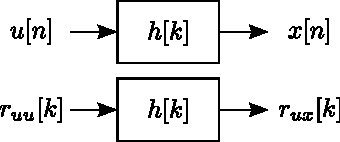
\includegraphics[width=0.9\textwidth]{figuras/problem_4_8_wss_filtrado.pdf}
  \end{minipage}\hfill
  \begin{minipage}[c]{0.56\textwidth}
    \caption{En un sistema lineal \(h[k]\), si la salida es el proceso \(x[n]\) cuando la entrada es el proceso \(u[n]\) WSS, la salida cuando la entrada es la autocorrelación de \(u[n]\) es la correlación cruzada entre la entrada y la salida.}\label{fig:problem_4_8_wss_filtrado}
  \end{minipage}
\end{figure}
Aplicando al transformada de Fourier, se obtiene la densidad espectral de potencia cruzada entre la entrada y la salida,
\[
 P_{ux}(f)=H(f)P_{uu}(f).
\]

Si la entrada es ruido blanco con PSD \(P_{uu}(f)=\sigma^2\)
\[
 P_{ux}(e^{j\omega})=H(e^{j\omega})\sigma^2,
\]
por lo que un estimador de la respuesta en frecuencia del filtro es
\[
\hat{H}(e^{j\omega})=\frac{P_{ux}(e^{j\omega})}{\sigma^2}=\frac{P_{ux}(e^{j\omega})}{r_{uu}[0]},
\]
ya que \(r_{uu}[k]=\sigma^2\delta[k]\) y por lo tanto, \(r_{uu}[0]=\sigma^2\).
Aplicando la antitransformada de Fourier, se obtiene la expresión en el dominio del tiempo, que es
\[
\mathbf{\hat{h}}=\frac{\mathbf{r}_{ux}}{r_{uu}[0]},
\]
coincidiendo con la ecuación \ref{eq:system_identification_h_opt_wn}.

Si \(P_{uu}(f)=0\) en una banda de frecuencias, \(P_{ux}(f)=0\) en la misma banda de frecuencias independientemente de \(H(f)\), y por lo tanto, no se dispone de información sobre \(H(f)\) en esa banda de frecuencias.


\subsection{Problema 9}\label{sec:problem_4_9}

Derivar las ecuaciones \ref{eq:linear_model_extension_mvu} y \ref{eq:linear_model_extension_mvu_covariance} del estimador MVU y la covarianza del estimador de la extensión del modelo lineal de forma análoga a la realizada en la sección \ref{sec:linear_model_definition}.

\paragraph{Solución} Los datos observados pueden modelarse como
\[
 \x=\Hbf\thetabf+\w,
\]
donde \(\w\sim\mathcal{N}(\mathbf{0},\C)\). El vector \(\x\) de observaciones es de dimensiones \(N\times1\), la matriz \(\Hbf\) conocida es de dimensiones \(N\times p\) con \(N>p\) y rango \(p\), el vector de parámetros a estimar \(\thetabf\) tiene  dimensiones \(p\times 1\), \(\w\) es ruido coloreado de dimensiones \(N\times 1\) con matriz de covarianza \(\C\) de dimensiones \(N\times N\).

Se verá si es posible factorizar la función de verosimilitud logarítmica como
\[
 \frac{\partial\ln p(\x;\,\thetabf)}{\partial\thetabf}=\I(\thetabf)(\g(\x)-\thetabf).
\]
En caso afirmativo, el estimador \(\hat{\thetabf}=\g(\x)\) es MVU y eficiente. La PDF de los datos es
\[
 p(\x;\,\thetabf)=\frac{1}{(2\pi)^\frac{N}{2}\det^\frac{1}{2}(\C)}\exp\left[-\frac{1}{2}(\x-\Hbf\thetabf)^T\C^{-1}(\x-\Hbf\thetabf)\right],
\]
y al tomar logaritmo se tiene que
\[
 \ln p(\x;\,\thetabf)=-\frac{N}{2}\ln(2\pi)-\frac{1}{2}\det(\C)-\frac{1}{2}(\x-\Hbf\thetabf)^T\C^{-1}(\x-\Hbf\thetabf).
\]
Luego, derivando respecto al parámetro, se obtiene que
\begin{align*}
 \frac{\partial p(\x,\,\thetabf)}{\partial\thetabf}&=-\frac{1}{2}\frac{\partial}{\partial\thetabf}\left[(\x-\Hbf\thetabf)^T\C^{-1}(\x-\Hbf\thetabf)\right]\\
 &=-\frac{1}{2}\frac{\partial}{\partial\thetabf}\left[(\x^T-\thetabf^T\Hbf^T)\C^{-1}(\x-\Hbf\thetabf)\right]\\
 &=-\frac{1}{2}\frac{\partial}{\partial\thetabf}\left[\x^T\C^{-1}\x-\x^T\C^{-1}\Hbf\thetabf-\thetabf^T\Hbf^T\C^{-1}\x+\thetabf^T\Hbf^T\C^{-1}\Hbf\thetabf\right]\\
 &=-\frac{1}{2}\frac{\partial}{\partial\thetabf}\left[\x^T\C^{-1}\x-2\x^T\C^{-1}\Hbf\thetabf+\thetabf^T\Hbf^T\C^{-1}\Hbf\thetabf\right].
\end{align*}
Para calcular la derivada, se procede de forma análoga a la realizada en la sección \ref{sec:linear_model_definition} definiendo el vector \(\bbf^T=\x^T\C^{-1}\Hbf\) y la matriz \(\A=\Hbf^T\C^{-1}\Hbf\) simétrica, y teniendo en cuenta que se cumple que
\[
 \frac{\partial \mathbf{b}^T\thetabf}{\partial\thetabf}=\mathbf{b},
 \qquad\frac{\partial \thetabf^T\mathbf{A}\thetabf}{\partial\thetabf}=2\mathbf{A}\thetabf,
\]
como se explica en el apéndice \ref{ap:derivatives_respect_vector}, se obtiene que
\[
 \frac{\partial p(\x,\,\thetabf)}{\partial\thetabf}=-\frac{1}{2}\left[-2\Hbf^T\C^{-1}\x+2\Hbf^T\C^{-1}\Hbf\thetabf\right]
 =\left[\Hbf^T\C^{-1}\x-\Hbf^T\C^{-1}\Hbf\thetabf\right],
\]
y asumiendo que \(\Hbf^T\C^{-1}\Hbf\) es invertible, se llega a que
\[
 \frac{\partial p(\x,\,\thetabf)}{\partial\thetabf}=\Hbf^T\C^{-1}\Hbf\left[\left(\Hbf^T\C^{-1}\Hbf\right)^{-1}\Hbf^T\C^{-1}\x-\thetabf\right],
\]
ecuación que está factorizada en la forma de la ecuación \ref{eq:crlb_efficiency_condition_vector} con
\begin{align*}
 \hat{\thetabf}&=\left(\Hbf^T\C^{-1}\Hbf\right)^{-1}\Hbf^T\C^{-1}\x\\
 \I(\thetabf)&=\Hbf^T\C^{-1}\Hbf.
\end{align*}
La matriz de covarianza del estimador es
\[
 \C_{\hat{\thetabf}}=\I^{-1}(\thetabf)=\left(\Hbf^T\C^{-1}\Hbf\right)^{-1}.
\]
Además, el estimador es eficiente y alcanza la CRLB. Observar que el resultado coincide con el obtenido mediante el enfoque de blanqueado de la sección \ref{sec:linear_model_coloured_noise_extension}.

\subsection{Problema 10}\label{sec:problem_4_10}

Si en el ejemplo de la sección \ref{sec:linear_model_dc_colored_noise} de la estimación del nivel de DC en ruido colorado las muestras de ruido son no correlacionadas pero con varianza distinta,
\[
 \C=\operatorname{diag}(\sigma_0^2,\dots,\,\sigma_{N-1}^2),
\]
calcular \(d_n\) e interpretar los resultados. ¿Qué pasaría con \(\hat{A}\) si una única varianza \(\sigma_n^2\) fuera cero?

\paragraph{Solución} Para calcular \(d_n\) (ecuación \ref{eq:linear_model_dc_colored_mvu_dn}), hay que factorizar \(\C^{-1}\) como \(\D^T\D\). Como la matriz de covarianza es diagonal, se cumple que
\[
 \C^{-1}=\operatorname{diag}\left(\frac{1}{\sigma_0^2},\dots,\,\frac{1}{\sigma_{N-1}^2}\right)
\]
y por lo tanto
\[
 \D=\operatorname{diag}\left(\frac{1}{\sigma_0},\dots,\,\frac{1}{\sigma_{N-1}}\right).
\]
Además,
\[
 \D\mathbf{1}=\left[\frac{1}{\sigma_0}\,\frac{1}{\sigma_1}\dots\frac{1}{\sigma_{N-1}}\right]^T
\]
por lo que \([\D\mathbf{1}]_n=1/\sigma_n\). Sustituyendo este resultado en la ecuación \ref{eq:linear_model_dc_colored_mvu_dn}, se obtiene que
\[
 d_n=\dfrac{\dfrac{1}{\sigma_n}}{\displaystyle\sum_{n=0}^{N-1}\dfrac{1}{\sigma_n^2}}.
\]
Los datos blanqueados \(\x'=\D\x\) quedan
\[
 x'[n]=\frac{x[n]}{\sigma_n},
\]
y se cumple que
\[
 \var(x'[n])=\frac{1}{\sigma^2_n}\var(x[n])=\frac{\sigma^2_n}{\sigma^2_n}=1.
\]
Como en este caso las muestras son no correlacionadas, el blanqueado lo único que hace es igualar las varianzas de todas las muestras al valor uno. Finalmente, sustituyendo estos resultados en la ecuación \ref{eq:linear_model_dc_colored_mvu}, el estimador MVU queda
\[
 \hat{A} = \dfrac{\displaystyle\sum_{n=0}^{N-1}\dfrac{1}{\sigma_n}x'[n]}{\displaystyle\sum_{n=0}^{N-1}\dfrac{1}{\sigma_n^2}}
 = \dfrac{\displaystyle\sum_{n=0}^{N-1}\dfrac{1}{\sigma^2_n}x[n]}{\displaystyle\sum_{n=0}^{N-1}\dfrac{1}{\sigma_n^2}}.
\]
Observar que el estimador le da mas importancia, a través del peso, a las muestras de menor varianza.

Considérese el caso en que la varianza de alguna muestra es nula, digamos, la de la muestra \(m\)-ésima. Como \(\sigma_m^2\to0\), el estimador es
\[
 \hat{A}=\dfrac{\displaystyle\sum_{n=0}^{N-1}\dfrac{1}{\sigma^2_n}x[n]}{\displaystyle\sum_{n=0}^{N-1}\dfrac{1}{\sigma_n^2}}
 \to\dfrac{\dfrac{1}{\sigma^2_m}x[m]}{\dfrac{1}{\sigma_m^2}}=x[m],
\]
como es de esperarse, ya que la muestra \(x[m]\), al tener ruido de varianza nula, no tiene error y por lo tanto, toma el valor del nivel de DC exacto.


\subsection{Problema 11}\label{sec:problem_4_11}

Considérese el modelo de datos descripto en el problema de la sección \ref{sec:problem_3_9}. Encontrar el estimador MVU de \(A\) y su varianza. ¿Porque el estimador es independiente de \(\rho\)? ¿Qué ocurre cuando \(\rho\to\pm1\)?

\paragraph{Solución} El modelo de los datos en notación matricial es
\[
 \x=\Hbf A+\w,\qquad \Hbf=[1\,1]^T,
\]
y el ruido \(\w\) es coloreado con matriz de covarianza
\[
 \C=\sigma^2
 \begin{bmatrix}
    1 & \rho\\
    \rho & 1
 \end{bmatrix}.
\]
Por tratarse del problema de estimación del nivel de DC en ruido coloreado, el estimador y su varianza fueron calculados en el ejemplo de la sección \ref{sec:linear_model_dc_colored_noise}, y son
\[
 \hat{A}=\frac{\mathbf{1}^T\C^{-1}\x}{\mathbf{1}^T\C^{-1}\mathbf{1}},
 \qquad \qquad
 \var(\hat{A})=\frac{1}{\mathbf{1}^T\C^{-1}\mathbf{1}}.
\]
La matriz de covarianza inversa es
\[
 \C^{-1}=\frac{1}{\sigma^2(1-\rho^2)}
 \begin{bmatrix}
    1 & -\rho\\
    -\rho & 1
 \end{bmatrix},
\]
y por lo tanto
\begin{align*}
  \mathbf{1}^T\C^{-1}\x&=
 \begin{bmatrix}
     1 & 1 
 \end{bmatrix}
 \frac{1}{\sigma^2(1-\rho^2)}
 \begin{bmatrix}
    1 & -\rho\\
    -\rho & 1
 \end{bmatrix}
 \begin{bmatrix}
    x[0]\\
    x[1]
 \end{bmatrix}\\
 &=\frac{1}{\sigma^2(1-\rho^2)}
 \begin{bmatrix}
     1 & 1 
 \end{bmatrix}
 \begin{bmatrix}
    x[0]-\rho x[1]\\
    -\rho x[0]+x[1]
 \end{bmatrix}\\
 &=\frac{x[0]-\rho x[1]-\rho x[0]+x[1]}{\sigma^2(1-\rho^2)}\\
 &=\frac{(1-\rho)(x[0]+x[1])}{\sigma^2(1-\rho^2)}.
\end{align*}
Sustituyendo en el resultado \(x[0]\) y \(x[1]\) por 1, se tiene que
\[
 \mathbf{1}^T\C^{-1}\mathbf{1}=\frac{2(1-\rho)}{\sigma^2(1-\rho^2)}.
\]
Por lo tanto,
\[
 \hat{A}=\frac{(1-\rho)(x[0]+x[1])}{2(1-\rho)}=\frac{x[0]+x[1]}{2}=\bar{\x},
\]
y
\[
 \var(\hat{A})=\frac{\sigma^2(1-\rho^2)}{2(1-\rho)}=\frac{\sigma^2}{2}(1+\rho).
\]

Para determinar porque el estimador no depende de \(\rho\), se observa que \(\Hbf\) es un vector propio de la matriz de covarianza \(\C\). Efectivamente,
\[
 \C\Hbf=\sigma^2
 \begin{bmatrix}
    1 & \rho\\
    \rho & 1
 \end{bmatrix}
 \begin{bmatrix}
    1\\
    1
 \end{bmatrix}
 =\sigma^2
 \begin{bmatrix}
    1+\rho\\
    1+\rho
 \end{bmatrix}
 =\sigma^2(1+\rho)
 \begin{bmatrix}
    1\\
    1
 \end{bmatrix}
 =\sigma^2(1+\rho)\Hbf,
\]
y por lo tanto se cumple que \(\C\Hbf=\lambda\Hbf\), donde el valor propio correspondiente al vector propio \(\Hbf\) es \(\lambda=\sigma^2(1+\rho)\). De esta forma, \(\Hbf\) también es un vector propio de \(\C^{-1}\) con valor propio \(1/\lambda\), es decir, se cumple que \(\C^{-1}\Hbf=(1/\lambda)\Hbf\) y el estimador se puede expresar como (ecuación \ref{eq:linear_model_extension_mvu})
\begin{align*}
 \hat{A}&=\left(\Hbf^T\C^{-1}\Hbf\right)^{-1}\Hbf^T\C^{-1}\x\\
  &=\left(\Hbf^T\C^{-1}\Hbf\right)^{-1}\left(\C^{-1}\Hbf\right)^T\x\\
  &=\left(\Hbf^T\frac{1}{\lambda}\Hbf\right)^{-1}\left(\frac{1}{\lambda}\Hbf\right)^T\x\\
  &=\lambda\left(\Hbf^T\Hbf\right)^{-1}\frac{1}{\lambda}\Hbf^T\x\\
  &=\left(\Hbf^T\Hbf\right)^{-1}\Hbf^T\x,
\end{align*}
que no depende de la matriz de covarianza \(\C\) y por lo tanto, tampoco del coeficiente de correlación \(\rho\). En el caso de estimación del nivel de DC en ruido coloreado, esto ocurre siempre que el vector \(\mathbf{1}\) sea vector propio de la matriz de covarianza \(\C\).  

En el problema de la sección \ref{sec:problem_3_9} se explica qué ocurre cuando \(\rho\to\pm1\).


\subsection{Problema 12}

En este problema se investiga la estimación de una función lineal de \(\thetabf\). Siendo este nuevo parámetro \(\alphabf=\A\thetabf\), donde \(\A\) es una matriz conocida \(r\times p\) con \(r<p\) y rango \(r\), mostrar que el estimador MVU es
\[
 \hat{\alphabf}=\A\hat{\thetabf},
\]
donde \(\hat{\thetabf}\) es el estimador MVU de \(\thetabf\). Además, calcular la matriz de covarianza. Sugerencia: reemplazar \(\x\) por
\[
 \x'=\A(\Hbf^T\Hbf)^{-1}\Hbf^T\x,
\]
donde \(\x'\) tiene tamaño \(r\times1\). Esto resulta en el \emph{modelo lineal reducido}. Se puede mostrar que \(\x'\) contiene toda la información sobre \(\thetabf\), por lo que es posible basar el estimador en este conjunto de datos de menor dimensión.

\paragraph{Solución} En el modelo lineal, el estimador MVU es (ecuación \ref{eq:linear_model_mvu})
\[
 \hat{\thetabf}=(\Hbf^T\Hbf)^{-1}\Hbf^T\x,
\]
por lo que el estimador de \(\alphabf\) es
\[
 \hat{\alphabf}=\A\hat{\thetabf}=\A(\Hbf^T\Hbf)^{-1}\Hbf^T\x.
\]
Una forma de verificar que \(\hat{\alphabf}\) es el estimador MVU de \(\alphabf\), es multiplicar el modelo lineal \(\x=\Hbf\thetabf+\w\) por \(\A(\Hbf^T\Hbf)^{-1}\Hbf^T\). Esto conduce a
\begin{align*}
 \A(\Hbf^T\Hbf)^{-1}\Hbf^T\x&=\A(\Hbf^T\Hbf)^{-1}\Hbf^T\Hbf\thetabf+\A(\Hbf^T\Hbf)^{-1}\Hbf^T\w\\
  &=\A\thetabf+\A(\Hbf^T\Hbf)^{-1}\Hbf^T\w\\
  &=\alphabf+\A(\Hbf^T\Hbf)^{-1}\Hbf^T\w,
\end{align*}
que es un nuevo modelo lineal,
\[
 \x'=\Hbf'\alphabf+\w',
\]
donde \(\x'=\A(\Hbf^T\Hbf)^{-1}\Hbf^T\x\) y \(\w'=\A(\Hbf^T\Hbf)^{-1}\Hbf^T\w\) tienen tamaño \(r\times1\), y \(\Hbf'=\I\) de tamaño \(r\times r\). En este modelo lineal, el ruido \(\w'\) es coloreado con matriz de covarianza
\begin{align*}
 \C_{\w'}&=E(\w'\w'^T)\\
  &=E\left[\A(\Hbf^T\Hbf)^{-1}\Hbf^T\w\w^T\Hbf{(\Hbf^T\Hbf)^{-1}}^T\A^T\right]\\
  &\overset{(a)}{=}\A(\Hbf^T\Hbf)^{-1}\Hbf^TE(\w\w^T)\Hbf(\Hbf^T\Hbf)^{-1}\A^T\\
  &\overset{(b)}{=}\sigma^2\A(\Hbf^T\Hbf)^{-1}\Hbf^T\Hbf(\Hbf^T\Hbf)^{-1}\A^T,
\end{align*}
donde en \((a)\) se tuvo en cuenta que \((\Hbf^T\Hbf)^{-1}\) es una matriz simétrica y en \((b)\) que el ruido en el modelo lineal convencional es blanco, y por lo tanto \(E(\w\w^T)=\C_{w}=\sigma^2\I\). 
Finalmente, eliminando una matriz y su inversa se obtiene que
\[
 \C_{\w'}=\sigma^2\A(\Hbf^T\Hbf)^{-1}\A^T.
\]
El estimador MVU está dado por la ecuación \ref{eq:linear_model_extension_mvu} del modelo lineal extendido, y es
\begin{align*}
 \boldsymbol{\hat{\alphabf}}&=\left(\Hbf'^T\C_{w'}^{-1}\Hbf'\right)^{-1}\Hbf'^T\C_{\w'}^{-1}\x'\\
  &\overset{(a)}{=}\x'\\
  &=\A(\Hbf^T\Hbf)^{-1}\Hbf^T\x,
\end{align*}
donde en \((a)\) se tuvo en cuenta que \(\Hbf'=\I\). Esto es lo que se quería demostrar.
La matriz de covarianza del estimador está dada por la ecuación \ref{eq:linear_model_extension_mvu_covariance}, y es
\begin{align*}
 \mathbf{C}_{\hat{\alphabf}}&=\left(\Hbf'^T\C_{\w'}^{-1}\Hbf'\right)^{-1}\\
   &=\C_{\w'}\\
   &=\sigma^2\A(\Hbf^T\Hbf)^{-1}\A^T.
\end{align*}

\subsection{Problema 13}

En la práctica a veces se encuentra el ``modelo lineal'' \(\x=\Hbf\thetabf+\w\) pero con la matriz \(\Hbf\) compuesta de variables aleatorias. Supóngase que se ignora esta diferencia y se emplea el estimador usual
\[
 \hat{\thetabf}=(\Hbf^T\Hbf)^{-1}\Hbf^T\x,
\]
donde se asume que la realización particular de \(\Hbf\) es conocida. Mostrar que si \(\Hbf\) y \(\w\) son independientes, la media y la covarianza de \(\hat{\thetabf}\) son
\begin{align*}
 E(\hat{\thetabf})&=\thetabf\\
 \C_{\hat{\thetabf}}&=\sigma^2E_H\left[(\Hbf^T\Hbf)^{-1}\right],
\end{align*}
donde \(E_H\) denota la esperanza respecto a la PDF de \(\Hbf\). ¿Qué sucede si no se asume la hipótesis de independencia?

\paragraph{Solución} Para calcular la esperanza, se observa que el estimador se puede escribir como
\begin{align}\label{eq:problem_4_13_estimator}
 \hat{\thetabf}&=(\Hbf^T\Hbf)^{-1}\Hbf^T\x\nonumber\\
  &=(\Hbf^T\Hbf)^{-1}\Hbf^T(\Hbf\thetabf+\w)\nonumber\\
  &=\thetabf+(\Hbf^T\Hbf)^{-1}\Hbf^T\w,
\end{align}
y por lo tanto, la esperanza es
\begin{align*}
 E(\hat{\thetabf})&=\thetabf+E\left[(\Hbf^T\Hbf)^{-1}\Hbf^T\w\right]\\
  &\overset{(a)}{=}\thetabf+E_H\left[(\Hbf^T\Hbf)^{-1}\Hbf^T\right]E(\w)\\
  &\overset{(b)}{=}\thetabf,
\end{align*}
donde en \((a)\) se empleó que \(\Hbf\) y \(\w\) son variables aleatorias independientes y en \((b)\) que \(E(\w)=0\) por ser ruido blanco. Se concluye que el estimador habitual es insesgado aunque los elementos de \(\Hbf\) sean variables aleatorias. La covarianza del estimador es
\begin{align*}
 \C_{\hat{\thetabf}}&=E\left[(\hat{\thetabf}-\thetabf)(\hat{\thetabf}-\thetabf)^T\right]\\
  &\overset{(a)}{=}E\left[(\Hbf^T\Hbf)^{-1}\Hbf^T\w\w^T\Hbf(\Hbf^T\Hbf)^{-1}\right]\\
  &\overset{(b)}{=}E_HE\left[(\Hbf^T\Hbf)^{-1}\Hbf^T\w\w^T\Hbf(\Hbf^T\Hbf)^{-1}\right]\\
  &\overset{(c)}{=}E_H\left[(\Hbf^T\Hbf)^{-1}\Hbf^TE(\w\w^T)\Hbf(\Hbf^T\Hbf)^{-1}\right]\\
  &\overset{(d)}{=}E_H\left[(\Hbf^T\Hbf)^{-1}\Hbf^T(\sigma^2\I)\Hbf(\Hbf^T\Hbf)^{-1}\right]\\
  &=\sigma^2E_H\left[(\Hbf^T\Hbf)^{-1}\right],
\end{align*}
donde en \((a)\) se empleó la identidad de la ecuación \ref{eq:problem_4_13_estimator} y en las identidades \((b)\), \((c)\) y \((d)\) se consideró la independencia de \(\Hbf\) y \(\w\). Para aclarar la notación utilizada, se realiza a continuación el mismo cálculo con las integrales explícitas de la esperanza,
\begin{align*}
 E\left[(\Hbf^T\Hbf)^{-1}\Hbf^T\w\w^T\Hbf(\Hbf^T\Hbf)^{-1}\right]&=
  \int_{-\infty}^{\infty}\int_{-\infty}^{\infty}(\Hbf^T\Hbf)^{-1}\Hbf^T\w\w^T\Hbf(\Hbf^T\Hbf)^{-1}p(\Hbf,\,\w)\,d\Hbf d\w\\
  &\overset{(a)}{=}
  \int_{-\infty}^{\infty}\int_{-\infty}^{\infty}(\Hbf^T\Hbf)^{-1}\Hbf^T\w\w^T\Hbf(\Hbf^T\Hbf)^{-1}p(\Hbf)p(\w)\,d\Hbf d\w\\
  &=
  \int_{-\infty}^{\infty}(\Hbf^T\Hbf)^{-1}\Hbf^T\left(\int_{-\infty}^{\infty}\w\w^Tp(\w)\,d\w\right)\Hbf(\Hbf^T\Hbf)^{-1}p(\Hbf)\,d\Hbf\\
  &\overset{(b)}{=}
  \int_{-\infty}^{\infty}(\Hbf^T\Hbf)^{-1}\Hbf^T\left(\sigma^2\I\right)\Hbf(\Hbf^T\Hbf)^{-1}p(\Hbf)\,d\Hbf\\
  &=
  \sigma^2\int_{-\infty}^{\infty}(\Hbf^T\Hbf)^{-1}p(\Hbf)\,d\Hbf\\
  &=\sigma^2E_H\left[(\Hbf^T\Hbf)^{-1}\right],
\end{align*}
donde en \((a)\) se consideró que \(\Hbf\) y \(\w\) son independientes y por lo tanto, la PDF conjunta es el producto de las PFD, \(p(\Hbf,\,\w)=p(\Hbf)p(\w)\) y en \((b)\) se tuvo en cuenta que la integral entre paréntesis es \(E(\w\w^T)=\C=\sigma^2\I\).

En el caso en que \(\Hbf\) y \(\w\) no son independientes, se cumple que
\begin{align*}
 E(\hat{\thetabf})&=\thetabf+E\left[(\Hbf^T\Hbf)^{-1}\Hbf^T\w\right]\\
 \C_{\hat{\thetabf}}&=E\left[(\Hbf^T\Hbf)^{-1}\Hbf^T\w\w^T\Hbf(\Hbf^T\Hbf)^{-1}\right].
\end{align*}
Como el término \(E\left[(\Hbf^T\Hbf)^{-1}\Hbf^T\w\right]\) en la esperanza del estimador no necesariamente es nulo, el estimador podría no ser insesgado. 


\subsection{Problema 14}

Supóngase que se observa una señal en ruido que está sujeta a desvanecerse. Se modela el proceso de devanecimiento como que la señal está presente o no está presente. Como ilustración sencilla, se considera el caso de la estimación del nivel de DC en WGN, o \(x[n]=A+w[n]\), \(n=0,\,\dots,\,N-1\). Cuando la señal se desvanece, el modelo de los datos es
\[
 x[n]=
\left\{ 
\begin{array}{l l}
    A+w[n] & n=0,\,\dots,\,M-1\\
    w[n] & n=M,\,\dots,\,N-1
\end{array} \right.
\]
donde la probabilidad de desvanecimiento es \(\epsilon\). Asumiendo que se conoce cuando la señal experimentó desvanecimiento, usar los resultados del problema anterior para determinar un estimador de \(A\) y también su varianza. Comparar los resultados en el caso en que no se produce desvanecimiento.

\paragraph{Solución} Asúmase que se observa una realización en donde se produce desvanecimiento en la muestra \(M\). Como se mostró en el problema anterior, si el proceso de desvanecimiento y el ruido son independientes, el estimador usual del modelo lineal es insesgado. Por lo tanto, el estimador es
\[
 \hat{A}=(\Hbf^T\Hbf)^{-1}\Hbf^T\x,\qquad\textrm{con}\qquad
 \Hbf=[\underset{0}{1}\;\dots\;\underset{M-1}{1}\;\underset{M}{0}\;\dots\;\underset{N-1}{0}]
\]
es decir, \(\Hbf\) es un vector con \(M\) unos seguidos de \(N-M\) ceros. De esta forma,
\[
 \hat{A}=\frac{1}{M}\sum_{n=0}^{M-1}x[n].
\]
Del problema anterior se tiene que la varianza es
\begin{align*}
 \var(\hat{A})&=\sigma^2E_H\left[(\Hbf^T\Hbf)^{-1}\right]\\
  &\overset{(a)}{=}\sigma^2\left[\frac{1}{N}(1-\epsilon)+\frac{1}{M}\epsilon\right]\\
  &=\frac{\sigma^2}{N}\left[1-\epsilon+\frac{N}{M}\epsilon\right]\\
  &=\frac{\sigma^2}{N}\left[1+\left(\frac{N}{M}-1\right)\epsilon\right]\\
  &\overset{(b)}{\geq}\frac{\sigma^2}{N}.
\end{align*}
donde en \((a)\) la esperanza es el valor que toma \((\Hbf^T\Hbf)^{-1}\) en el caso en que no hay desvanecimiento por la probabilidad de que no haya  desvanecimiento sumado al valor que toma cuando hay desvanecimiento por la probabilidad de que haya desvanecimiento y la desigualdad en \((b)\) proviene de que \(N\geq M\). Notar que la igualdad se da en el caso en que \(M=N\) o que \(\epsilon=0\), que es que no hay desvanecimiento.


\chapter{Estimación insesgada de varianza mínima general}

\section{Factorización de Neyman-Fisher}

El teorema de la factorización de Neyman-Fisher es una herramienta poderosa para encontrar estadísticos suficientes de un parámetro. 

\subsection{Teorema}

Si la PDF \(p(\x;\,\theta)\) de los datos puede ser factorizada como
\begin{equation}\label{eq:general_mvu_neyman_fisher_factorization}
  p(\x;\,\theta)=g(T(\x),\,\theta)h(\x),
\end{equation}
donde \(g\) es una función que depende de \(\x\) solo a través de \(T(\x)\) y \(h\) es una función que depende solo de los datos \(\x\), se cumple que \(T(\x)\) es un estadístico suficiente de \(\theta\). Recíprocamente, si \(T(\x)\) es un estadístico suficiente de \(\theta\), la PDF de los datos puede ser factorizada como en la ecuación \ref{eq:general_mvu_neyman_fisher_factorization}.

\paragraph{Demostración} Para la demostración, se realizarán primero dos observaciones:
\begin{itemize}
 \item Considérese la PDF conjunta \(p(\x,\,T(\x);\,\theta)\). Para evaluar esta PDF, debe tenerse en cuenta que \(T(\x)\) es funcionalmente dependiente de \(\x\). Por lo tanto, la PDF conjunta debe ser nula en todo \(\x=\x_0\), \(T(\x)=T_0\) a menos que \(T(\x_0)=T_0\). Esto implica que 
 \begin{equation}\label{eq:general_mvu_statistic_join_pdf}
  p(\x,\,T(\x);\,\theta)=p(\x;\,\theta)\delta({T(\x)-T_0}).
 \end{equation}
 Una analogía es por ejemplo el caso en que una variable aleatoria \(x\) escalar toma siempre el mismo valor, digamos \(c\). En ese caso, \(x\) tiene una distribución de probabilidad degenerada\footnote{Ver: \url{https://en.wikipedia.org/wiki/Degenerate_distribution}}
 \[\def\arraystretch{1.2}
 F_c(x)=
 \left\{\begin{array}{ll}
  0, &  x<c\\
  1, &  x\geq c
 \end{array}\right.,
\]
por lo que la PDF es \(p(x)=\delta(x-c)\). Otra analogía mas cercana a la situación de interés es cuando se tienen dos variables aleatorias escalares \(x\) y \(y\) tales que \(x=y\) siempre. La PDF conjunta es \(p(x,\/y)=p(x)\delta(y-x)\), una PDF degenerada de dos variables.
 \item Una forma de representar la PDF de una función de varias variables es la siguiente: si \(y=g(\x)\), donde \(\x\) es una variable aleatoria vectorial, la PDF puede expresarse como
 \begin{equation}\label{eq:general_mvu_rv_transformation}
  p(y)=\int p(\x)\delta(y-g(\x))\,d\x.
 \end{equation}
 Se mostrará para el caso escalar que esto es equivalente a la ecuación usual de la PDF de una variable aleatoria transformada. Si \(x\) es una variable aleatoria escalar, la PDF de la variable transformada \(y=g(x)\) es (ver el capítulo 5 de \cite{papoulis2002probability})
 \begin{equation}\label{eq:pdf_transformed_rv}
  p_y(y)=\sum_{i=1}^k\frac{p_x(x_i)}{|g'(x_i)|},
 \end{equation}
 donde \(\{x_1,\,x_2,\,\dots,\,x_k\}\) son las soluciones de \(y=g(x)\), es decir, \(y=g(x_1)=g(x_2)=\cdots =g(x_k)\). Para demostrar la equivalencia con la ecuación \ref{eq:general_mvu_rv_transformation}, se verá primero que 
 \begin{equation}\label{eq:general_mvu_delta_of_a_function}
  \delta(y-g(x))=\sum_{i=1}^k\frac{\delta(x-x_i)}{|g'(x_i)|}.
 \end{equation}
 Un resultado mas general, es que 
 \[
  \int_{-\infty}^{\infty}\delta(g(x))f(x)\,dx=\sum_{i=1}^k\frac{f(x_i)}{|g'(x_i)|}.
 \]
 Efectivamente\footnote{Esta prueba está basada en \url{https://math.stackexchange.com/questions/276583/dirac-delta-function-of-a-function}.},
 \begin{align*}
  \int_{-\infty}^{\infty}\delta(g(x))f(x)\,dx&\overset{(a)}{=}\sum_{i=1}^k\int_{x_i-\epsilon_i}^{x_i+\epsilon_i}\delta(g(x))f(x)\,dx\\
  &\overset{(b)}{=}\sum_{i=1}^k\int_{g(x_i-\epsilon_i)}^{g(x_i+\epsilon_i)}\delta(u)f(g^{-1}(u))\frac{1}{g'(g^{-1}(u))}\,du\\
  &\overset{(c)}{=}\sum_{i=1}^k\frac{f(x_i)}{g'(x_i)}\int_{g(x_i-\epsilon_i)}^{g(x_i+\epsilon_i)}\delta(u)\,du\\
  &\overset{(d)}{=}\sum_{i=1}^k\frac{f(x_i)}{|g'(x_i)|},
 \end{align*}
donde en \((a)\) los \(x_i\) son las raíces de \(g\) y se consideró que \(\delta(g(x))=0\) excepto cuando \(g(x)=0\) y por lo tanto, es equivalente considerar el dominio de integración solo en torno a los puntos \(x_i\) donde \(g(x_i)=0\), en \((b)\) se realizó el cambio de variable \(u=g(x)\) y por lo tanto \(x=g^{-1}(u)\) y \(dx=[g^{-1}(u)]'du=du/g'(g^{-1}(u))\), donde en la última igualdad se empleó el teorema de la función inversa\footnote{Ver \url{https://en.wikipedia.org/wiki/Inverse_function_theorem}, por ejemplo.}, en \((c)\) se evaluó la función que multiplica a la delta en \(u=g(x_i)\), que es el único punto en donde \(\delta(u)\) es distinto de cero en el intervalo de integración, y en \((d)\) se consideró que si \(g'(x_i)<0\), \(g(x_i-\epsilon_i)>g(x_i+\epsilon_i)\), y hay que invertir los límites de integración y cambiar el signo de la integral.
Además, se observa que
\begin{align*}
  \sum_{i=1}^k\frac{f(x_i)}{|g'(x_i)|}&=\sum_{i=1}^k\int_{-\infty}^{\infty}\frac{f(x)\delta(x-x_i)}{|g'(x_i)|}\,dx\\
  &=\int_{-\infty}^{\infty}\left(\sum_{i=1}^k\frac{\delta(x-x_i)}{|g'(x_i)|}\right)f(x)\,dx,
 \end{align*}
concluyendo que 
\[
 \delta(g(x))=\sum_{i=1}^k\frac{\delta(x-x_i)}{|g'(x_i)|},
\]
que es la ecuación \ref{eq:general_mvu_delta_of_a_function}. Con esto, es posible mostrar que la ecuación \ref{eq:general_mvu_rv_transformation} es equivalente a la ecuación de la PDF de una variable aleatoria transformada. Basta sustituir le ecuación \ref{eq:general_mvu_delta_of_a_function} en la ecuación \ref{eq:general_mvu_rv_transformation}, resultando en
\begin{align*}
 p(y)&=\int_{-\infty}^{\infty} p(x)\delta(y-g(x))\,dx\\
  &=\int_{-\infty}^{\infty} p(x)\sum_{i=1}^k\frac{\delta(x-x_i)}{|g'(x_i)|}\,dx\\
  &=\sum_{i=1}^k\frac{p(x_i)}{|g'(x_i)|}\int_{-\infty}^{\infty}\delta(x-x_i)\,dx\\
  &=\sum_{i=1}^k\frac{p(x_i)}{|g'(x_i)|},
\end{align*}
que es lo que se quería mostrar.
\end{itemize}

Se comenzará la demostración del teorema de la factorización de Neyman-Fisher probando que \(T(\x)\) es un estadístico suficiente si la factorización puede realizarse. Hay que demostrar que si la factorización se cumple, la probabilidad condicional de los datos dado el estadístico no depende del parámetro. Por el teorema de la probabilidad total, la probabilidad condicional es
\begin{align*}
 p(\x\,|\,T(\x)=T_0;\,\theta)&=\frac{p(\x,\,T(\x)=T_0;\,\theta)}{p(T(\x)=T_0;\,\theta)}\\
  &=\frac{p(\x;\,\theta)\delta(T(\x)-T_0)}{p(T(\x)=T_0;\,\theta)},
\end{align*}
donde en la segunda igualdad se empleó la observación realizada arriba. Aplicando la factorización (ecuación \ref{eq:general_mvu_neyman_fisher_factorization}), que se asume que se cumple por hipótesis, se tiene que
\begin{align*}
 p(\x\,|\,T(\x)=T_0;\,\theta)&=\frac{g(T(\x),\,\theta)h(\x)\delta(T(\x)-T_0)}{p(T(\x)=T_0;\,\theta)}\\
  &=\frac{g(T(\x)=T_0,\,\theta)h(\x)\delta(T(\x)-T_0)}{p(T(\x)=T_0;\,\theta)},
\end{align*}
donde en la segunda igualdad se aplicó la propiedad de la delta que indica que \(g(x)\delta(x-x_i)=g(x_i)\delta(x-x_i)\). Además, el denominador es
\begin{align*}
 p(T(\x)=T_0;\,\theta)&\overset{(a)}{=}\int p(\x;\,\theta)\delta(T(\x)-T_0)\,d\x\\
 &\overset{(b)}{=}\int g(T(\x)=T_0,\,\theta)h(\x)\delta(T(\x)-T_0)\,d\x\\
 &\overset{(c)}{=}g(T(\x)=T_0,\,\theta)\int h(\x)\delta(T(\x)-T_0)\,d\x,
\end{align*}
donde en \((a)\) se empleó la ecuación \ref{eq:general_mvu_rv_transformation}, en \((b)\) se aplicó nuevamente la factorización de la ecuación \ref{eq:general_mvu_neyman_fisher_factorization} y en \((c)\) se consideró que la integral es cero excepto en la superficie en \(\mathbb{R}^N\) donde \(T(\x)=T_0\), y \(g\) es constante en dicha superficie. Sustituyendo el resultado en la ecuación de la esperanza condicional, se obtiene que
\[
 p(\x\,|\,T(\x)=T_0;\,\theta)=\frac{h(\x)\delta(T(\x)-T_0)}{\int h(\x)\delta(T(\x)-T_0)\,d\x},
\]
que no depende de \(\theta\), como se quería demostrar. Se concluye que \(T(\x)\) es un estadístico suficiente.

Se probará ahora el recíproco: si \(T(\x)\) es un estadístico suficiente, la factorización puede realizarse. La PDF conjunta es
\begin{equation}\label{eq:general_mvu_joint_pdf}
 p(\x,\,T(\x)=T_0;\,\theta)=p(\x\,|\,T(\x)=T_0;\,\theta)p(T(\x)=T_0;\,\theta).
\end{equation}
Como se observó previamente, el lado derecho de la igualdad puede expresarse como
\[
 p(\x,\,T(\x)=T_0;\,\theta)=p(\x;\,\theta)\delta(T(\x)-T_0).
\]
Además, como \(T(\x)\) es un estadístico suficiente, la PDF condicional no depende del parámetro \(\theta\) y por lo tanto es \(p(\x\,|\,T(\x)=T_0)\). Sustituyendo estos resultados en la ecuación \ref{eq:general_mvu_joint_pdf}, se tiene que
\begin{equation}\label{eq:general_mvu_joint_pdf_tmp1}
 p(\x;\,\theta)\delta(T(\x)-T_0)=p(\x\,|\,T(\x)=T_0)p(T(\x)=T_0;\,\theta).
\end{equation}
La PDF condicional es nula excepto en la superficie de \(\mathbb{R}^N\) donde \(T(\x)=T_0\), y por lo tanto,
\[
 p(\x\,|\,T(\x)=T_0)=w(\x)\delta(T(\x)-T_0)
\]
con
\begin{equation}\label{eq:general_mvu_w_condition_tmp}
 \int w(\x)\delta(T(\x)-T_0)\,d\x=1
\end{equation}
para que se trate de una densidad de probabilidad.
Sustituyendo en la ecuación \ref{eq:general_mvu_joint_pdf_tmp1}, se obtiene que
\[
 p(\x;\,\theta)\delta(T(\x)-T_0)=w(\x)\delta(T(\x)-T_0)p(T(\x)=T_0;\,\theta),
\]
y definiendo 
\[
 w(\x)=\frac{h(\x)}{\int h(\x)\delta(T(\x)-T_0)\,d\x}
\]
de forma que se cumpla la condición de la ecuación \ref{eq:general_mvu_w_condition_tmp} se obtiene que
\[
 p(\x;\,\theta)\delta(T(\x)-T_0)=\frac{h(\x)\delta(T(\x)-T_0)}{\int h(\x)\delta(T(\x)-T_0)\,d\x}p(T(\x)=T_0;\,\theta)
\]
o
\[
 p(\x;\,\theta)=g(T(\x)=T_0;\,\theta)h(\x)
\]
con
\[
 g(T(\x)=T_0;\,\theta)=\frac{p(T(\x)=T_0;\,\theta)}{\int h(\x)\delta(T(\x)-T_0)\,d\x},
\]
que es lo que se quería demostrar. Además, en principio, la PDF del estadístico suficiente puede obtenerse de la factorización como
\[
 p(T(\x)=T_0;\,\theta)=g(T(\x)=T_0;\,\theta)\int h(\x)\delta(T(\x)-T_0)d\x.
\]

\subsection{Ejemplo: nivel de DC en WGN}\label{sec:general_mvu_dc_in_wgn_sufficient}

Se buscará un estadístico suficiente para el problema de la estimación del nivel de DC en WGN. Como se vió previamente, la PDF de los datos es (ecuación \ref{eq:dc_in_wgn_pdf})
\[
 p(\x;\,A)=\frac{1}{(2\pi\sigma^2)^\frac{N}{2}}\exp\left[-\frac{1}{2\sigma^2}\sum_{n=0}^{N-1}(x[n]-A)^2\right].
\]
Para demostrar que existe una factorización, se observa que el exponente se puede escribir como
\[
 \sum_{n=0}^{N-1}(x[n]-A)^2=\sum_{n=0}^{N-1}(x^2[n]-2Ax[n]+A^2)
  =\sum_{n=0}^{N-1}x^2[n]-2A\sum_{n=0}^{N-1}x[n]+NA^2,
\]
por lo que la PDF se factoriza como
\[
 p(\x;\,A)=\underbrace{\frac{1}{(2\pi\sigma^2)^\frac{N}{2}}\exp\left[-\frac{1}{2\sigma^2}\left(NA^2-2A\sum_{n=0}^{N-1}x[n]\right)\right]}_{\displaystyle g(T(\x),\,A)}\underbrace{\exp\left[-\frac{1}{2\sigma^2}\sum_{n=0}^{N-1}x^2[n]\right]}_{\displaystyle h(\x)}.
\]
Se concluye que \(T(\x)=\sum_{n=0}^{N-1}x[n]\) es un estadístico suficiente de \(A\). Notar que \(T'(\x)=2\sum_{n=0}^{N-1}x[n]\) también es un estadísticio suficiente de \(A\), y de hecho, cualquier función uno a uno de \(\sum_{n=0}^{N-1}x[n]\) también es un estadístico suficiente. Por lo tanto, los estadísiticos suficientes son únicos a menos de transformaciones inyectivas.

\subsection{Ejemplo: fase de una sinusoide}\label{sec:general_mvu_sinusoidal_phase_statistic}

Se considera el problema de la estimación de la fase \(\phi\) de una sinusoide en WGN,
\[
 x[n]=A\cos(2\pi f_0 n+\phi)+w[n],\qquad n=0,\,\dots,\,N-1,
\]
donde la amplitud \(A\) y la frecuencia \(f_0\) de la sinusoide son conocidas, así como la varianza \(\sigma^2\) del ruido. La PDF de los datos es
\[
 p(\x,\,\phi)=\frac{1}{(2\pi\sigma^2)^\frac{N}{2}}\exp\left\{-\frac{1}{2\sigma^2}\sum_{n=0}^{N-1}[x[n]-A\cos(2\pi f_0n+\phi)]^2\right\}.
\]
El exponente se puede expandir como
\begin{align*}
  \sum_{n=0}^{N-1}[x[n]-A(\cos2\pi f_0n+\phi)]^2
   &=\sum_{n=0}^{N-1}x^2[n]-2A\sum_{n=0}^{N-1}x[n]\cos(2\pi f_0n+\phi)+A^2\sum_{n=0}^{N-1}\cos^2(2\pi f_0n+\phi)\\
   &\overset{(a)}{=}\sum_{n=0}^{N-1}x^2[n]-2A\left(\sum_{n=0}^{N-1}x[n]\cos2\pi f_0n\right)\cos\phi\\
   &\qquad+2A\left(\sum_{n=0}^{N-1}x[n]\sin2\pi f_0n\right)\sin\phi+A^2\sum_{n=0}^{N-1}\cos^2(2\pi f_0n+\phi),
\end{align*}
donde en \((a)\) se empleó la identidad trigonométrica \(\cos(\alpha+\beta)=\cos\alpha\cos\beta-\sin\alpha\sin\beta\). En este ejemplo, no parece que la PDF se pueda factorizar como requiere el teorema de Neyman-Fisher, y por lo tanto, no existe un estadístico suficiente \emph{individual}. Sin embargo, la PDF se puede factorizar como
\begin{align*}
 p(\x,\,\phi)&=\underbrace{\frac{1}{(2\pi\sigma^2)^\frac{N}{2}}\exp\left\{-\frac{1}{2\sigma^2}\left[A^2\sum_{n=0}^{N-1}\cos^2(2\pi f_0n+\phi)-2AT_1(\x)\cos\phi+2AT_2(\x)\sin\phi\right]\right\}}_{\displaystyle g(T_1(\x),\,T_2(\x),\,\phi)}\\
 &\qquad\times\underbrace{\exp\left[-\frac{1}{2\sigma^2}\sum_{n=0}^{N-1}x^2[n]\right]}_{\displaystyle h(\x)},
\end{align*}
donde
\begin{equation}\label{eq:general_mvu_sinusoidal_phase_statistics}
 \begin{aligned}
  T_1(\x)&=\sum_{n=0}^{N-1}x[n]\cos2\pi f_0n\\
  T_2(\x)&=\sum_{n=0}^{N-1}x[n]\sin2\pi f_0n.
 \end{aligned}
\end{equation}
En este caso, una generalización del teorema de Neyman-Fisher indica que los estadísticos \(T_1(\x)\) y \(T_2(\x)\) son \emph{conjuntamente suficientes} para la estimación de \(\phi\). Sin embrago, no existe un estadístico suficiente individual en este caso.

\paragraph{Estadísticos conjuntamente suficientes} El concepto de estadísticos conjuntamente suficientes es una extensión de la definición de estadístico suficiente. Se dice que los \(r\) estadísticos \(T_1(\x),\,\dots,\,T_r(\x)\) son conjuntamente suficientes si la PDF condicional \(p(\x\,|\,T_1(\x),\,\dots,\,T_r(\x);\,\theta)\) de los datos no depende de \(\theta\). La generalización del teorema de la factorización de Neyman-Fisher indica que si \(p(\x;\,\theta)\) puede ser factorzada como
\[
 p(\x;\,\theta)=g(T_1(\x),\,\dots,\,T_r(\x),\,\theta)h(\x)
\]
se cumple que \(\{T_1(\x),\,\dots,\,T_r(\x)\}\) son estadísticos suficientes de \(\theta\).


\section{Uso del estadístico suficiente para encontrar el estimador MVU}

Asumiendo que se ha encontrado un estadístico suficiente \(T(\x)\) del parámetro \(\theta\), se puede usar el teorema de Rao-Blackwell-Lehmann-Scheffe (RBLS) para encontrar el estimador MVU. El enfoque se ilustra mediante un ejemplo.

\subsection{Ejemplo: nivel de DC en WGN}\label{sec:general_mvu_dc_in_wgn_estimator}

En el ejemplo de la sección \ref{sec:general_mvu_dc_in_wgn_sufficient} se encontró un estadístico suficiente para el nivel \(A\) de DC y se quiere encontrar el estimador \(\hat{A}\) MVU. Hay dos procedimientos distintos para encontrar \(\hat{A}\) en base al estadístico suficiente \(T(\x)=\sum_{n=0}^{N-1}x[n]\):
\begin{enumerate}
 \item Encontrar cualquier estimador insesgado de \(A\), por ejemplo, \(\check{A}=x[0]\), y determinar \(\hat{A}=E(\check{A}\,|\,T)\). La esperanza se toma respecto a \(p(\check{A}\,|\,T)\).
 \item Encontrar alguna función \(g\) de forma que \(\hat{A}=g(T)\) sea un estimador insesgado de \(A\).
\end{enumerate}
Para hacerlo mediante el primer procedimiento, sea \(\check{A}=x[0]\), y hay que determinar \(\hat{A}=E(x[0]\,|\,\sum_{n=0}^{N-1}x[n])\). Para calcular la esperanza condicional se necesitará la siguiente propiedad la PDF gaussiana condicional: si \([x\,y]^T\) es un vector gaussiano de media \(\mubf=[E(x)\,E(y)]^T\) y matriz de covarianza 
\[
 \C=
 \begin{bmatrix}
  \var(x) & \cov(x,\,y)\\
  \cov(y,\,x) & \var(y) 
 \end{bmatrix},
\]
se puede demostrar que (ver el apéndice \ref{ap:conditional_pdf_joint_gaussian})
\begin{align}\label{eq:conditional_mean_joint_gaussian}
 E(x\,|\,y)&=\int_{-\infty}^{\infty}xp(x\,|\,y)dx\nonumber\\
   &=E(x)+\frac{\cov(x,\,y)}{\var(y)}(y-E(y)).
\end{align}
Con \(x=x[0]\) y \(y=\sum_{n=0}^{N-1}x[n]\) se observa que
\[
 \begin{bmatrix}
  x\\
  y
 \end{bmatrix}=
 \begin{bmatrix}
  x[0]\\
  \displaystyle\sum_{n=0}^{N-1}x[n]
 \end{bmatrix}=
 \underbrace{\begin{bmatrix}
  1 & 0 & 0 & \dots & 1\\
  1 & 1 & 1 & \dots & 1
 \end{bmatrix}}_{\displaystyle\mathbf{L}}
 \begin{bmatrix}
  x[0]\\
  x[1]\\
  \vdots\\
  x[N-1]
 \end{bmatrix}.
\]
Esto implica que la PDF de \([x,\,y]^T\) es \(\mathcal{N}(\mubf,\,\C)\) por tratarse de una transformación lineal de un vector gaussiano, donde la media es
\[
 \mubf=E(\mathbf{L}\x)=\mathbf{L}E(\x)=\mathbf{L}A\mathbf{1}=
 \begin{bmatrix}
  A\\
  NA
 \end{bmatrix},
\]
y la matriz de covarianza es
\begin{align*}
 \C&=E\left\{[\mathbf{L}\x-E(\mathbf{L}\x)][\mathbf{L}\x-E(\mathbf{L}\x)]^T\right\}\\
   &=E\left\{\mathbf{L}[\x-E(\x)][\x-E(\x)]^T\mathbf{L}^T\right\}\\
   &=\mathbf{L}E\left\{[\x-E(\x)][\x-E(\x)]^T\right\}\mathbf{L}^T\\
   &=\mathbf{L}\left(\sigma^2\I\right)\mathbf{L}^T\\
   &=\sigma^2\mathbf{L}\mathbf{L}^T\\
   &=\sigma^2
   \begin{bmatrix}
    1 & 1\\
    1 & N
   \end{bmatrix}.
\end{align*}
Por lo tanto, aplicando el resultado de la ecuación \ref{eq:conditional_mean_joint_gaussian} con \(E(x)=A\), \(E(y)=N\), \(\cov(x,\,y)=\sigma^2\) y \(\var(y)=N\sigma^2\)
\begin{align*}
 \hat{A}&=E\left(x[0]\,\Bigg|\,\sum_{n=0}^{N-1}x[n]\right)\\
   &=A+\frac{\sigma^2}{N\sigma^2}\left(\sum_{n=0}^{N-1}x[n]-NA\right)\\
   &=\frac{1}{N}\sum_{n=0}^{N-1}x[n],
\end{align*}
se obtiene la media muestral, que es el estimador MVU. Este enfoque, que requiere el cálculo de la media condicional, suele ser matemáticamente intratable.

El segundo enfoque consiste en encontrar una función \(g\) de forma que 
\[
 \hat{A}=g\left(\sum_{n=0}^{N-1}x[n]\right)
\]
sea un estimador insesgado de \(A\). Como en este caso \(E(\sum_{n=0}^{N-1}x[n])=NA\), eligiendo \(g(x)=x/N\) se obtiene
\[
 \hat{A}=\frac{1}{N}\sum_{n=0}^{N-1}x[n]
\]
como el estimador MVU. Este enfoque suele ser mucho mas fácil de aplicar y es el que se emplea generalmente en la práctica.

\subsection{Teorema de Rao-Blackwell-Lehmann-Scheffe}

Si \(\check{\theta}\) es un estimador insesgado de \(\theta\) y \(T(\x)\) es un estadístico suficiente de \(\theta\), se cumple que \(\hat{\theta}=E(\check{\theta}\,|\,T(\x))\) es
\begin{enumerate}
 \item un estimador válido de \(\theta\), en el sentido de que no depende de \(\theta\).
 \item insesgado
 \item de menor varianza que \(\check{\theta}\), para todo \(\theta\)
\end{enumerate}
Además, si el estadístico es \emph{completo}, \(\hat{\theta}\) es el estimador MVU.

\paragraph{Demostración}

Para demostrar (1), se observa que
\begin{equation}\label{eq:general_mvu_rbls_estimator}
 \begin{aligned}
  \hat{\theta}&=E(\check{\theta}\,|\,T(\x))\\
   &=\int\check{\theta}(\x)p(\x\,|\,T(\x);\,\theta)\,d\x,
 \end{aligned}
\end{equation}
donde la segunda igualdad proviene de que \(E(g(x))=\int g(x)p(x)\,dx\). Por la definición de estadístico suficiente, \(p(\x\,|\,T(\x);\,\theta)\) no depende de \(\theta\), depende únicamente de \(\x\) y \(T(\x)\). De esta forma, al integrar en \(\x\), el resultado será únicamente una función de \(T\) y como consecuencia, solo de \(\x\). Se concluye que el estimador es válido por no depender de \(\theta\).

La afirmación (2) indica que \(E(\hat{\theta})=\theta\). Para demostrarlo, se considera que, como se dedujo previamente, \(\hat{\theta}\) es únicamente función de \(T\), y por lo tanto,
\begin{align*}
 E(\hat{\theta})&=\int \hat{\theta}(T)p(T(\x);\,\theta)\,dT\\
  &\overset{(a)}{=}\iint\check{\theta}(\x)p(\x\,|\,T(\x);\,\theta)\,d\x\,p(T(\x);\,\theta)\,dT\\
  &\overset{(b)}{=}\int\check{\theta}(\x)\int p(\x,\,T(\x);\,\theta)\,dTd\x\\
  &\overset{(c)}{=}\int\check{\theta}(\x)p(\x;\,\theta)d\x\\
  &=E(\check{\theta}),
\end{align*}
donde en \((a)\) se uso la ecuación \ref{eq:general_mvu_rbls_estimator}, en \((b)\) se tuvo en cuenta que \(p(x\,|\,y)p(y)=p(x,\,y)\) y en \((c)\) que \(\int p(x,\,y)\,dy=p(x)\). Como \(\check{\theta}\) es insesgado por hipótesis, se cumple que
\[
 E(\hat{\theta})=E(\check{\theta})=\theta,
\]
concluyendo que \(\hat{\theta}\) es insesgado.

Para probar (3) se observa que
\begin{align*}
 \var(\check{\theta})&=E\left[(\check{\theta}-E(\check{\theta}))^2\right]\\
   &=E\left[(\check{\theta}-\hat{\theta}+\hat{\theta}-\theta)^2\right]\\
   &=E\left[(\check{\theta}-\hat{\theta})^2\right]+
    2E\left[(\check{\theta}-\hat{\theta})(\hat{\theta}-\theta)\right]+
    E\left[(\hat{\theta}-\theta)^2\right].
\end{align*}
Se demostrará que el término cruzado \(E\left[(\check{\theta}-\hat{\theta})(\hat{\theta}-\theta)\right]\) es nulo. Por definición, \(\hat{\theta}\) es únicamente función de \(T\) y por lo tanto, la esperanza del término cruzado es respecto a la PDF conjunta de \(\check{\theta}\) y \(T\). De esta forma,
\begin{align*}
 E_{T,\,\check{\theta}}\left[(\check{\theta}-\hat{\theta})(\hat{\theta}-\theta)\right]&=E_TE_{\check{\theta}\,|\,T}\left[(\check{\theta}-\hat{\theta})(\hat{\theta}-\theta)\right].
\end{align*}
Pero
\begin{align*}
 E_{\check{\theta}\,|\,T}\left[(\check{\theta}-\hat{\theta})(\hat{\theta}-\theta)\right]&\overset{(a)}{=}E_{\check{\theta}\,|\,T}\left[(\check{\theta}-\hat{\theta})\right](\hat{\theta}-\theta)\\
  &\overset{(b)}{=}\left[E_{\check{\theta}\,|\,T}(\check{\theta}\,|\,T)-\hat{\theta}\right](\hat{\theta}-\theta)\\
  &\overset{(c)}{=}(\hat{\theta}-\hat{\theta})(\hat{\theta}-\theta)\\
  &=0,
\end{align*}
donde en \((a)\) y \((b)\) se empleó que como \(\hat{\theta}\) es función de \(T\) se cumple que \(E(\hat{\theta}\,|\,T)=\hat{\theta}\) y en \((c)\) la definición de \(\hat{\theta}\). Finalmente, se tiene que
\begin{align*}
 \var(\check{\theta})&=E\left[(\check{\theta}-\hat{\theta})^2\right]+
    E\left[(\hat{\theta}-\theta)^2\right]\\
    &=E\left[(\check{\theta}-\hat{\theta})^2\right]+\var(\hat{\theta})\\
    &\geq \var(\hat{\theta}).
\end{align*}
Falta ver que si \(T(\x)\) es completo, \(\hat{\theta}=E(\check{\theta}\,|\,T(\x))\) es el estimador MVU. Un estadístico es completo si existe solo una función del estadístico que lo hace insesgado. \(E(\check{\theta}\,|\,T(\x))\) es un estimador insesgado y de menor varianza que el estimador \(\check{\theta}\). Como \(E(\check{\theta}\,|\,T(\x))\) es una función únicamente de \(T(\x)\) ya que
\[
 \hat{\theta}=E(\check{\theta}\,|\,T(\x))=\int\check{\theta}p(\check{\theta}\,|\,T(\x))\,d\check{\theta}=g(T(\x)),
\]
y si \(T(\x)\) es completo, existe solo una función de \(T\) que es un estimador insesgado, \(\hat{\theta}\) es único independientemente del estimador \(\check{\theta}\) insesgado que se elija. Es decir, cualquier estimador \(\check{\theta}\) insesgado se mapea en el mismo estimador \(\hat{\theta}\). Como la varianza de \(\hat{\theta}\) es menor que la de cualquier estimador \(\check{\theta}\) insesgado, se concluye que \(\hat{\theta}\) debe ser el estimador MVU.

Se puede demostrar que un estadístico suficiente es completo si se cumple que
\[
 \int_{-\infty}^{\infty}v(T)p(T;\,\theta)\,dT=0,\qquad \forall\,\theta
\]
únicamente para la función \(v\) nula o \(v(T)=0\) para todo T (ver \cite{papoulis2002probability}).

\subsection{Ejemplo: media de ruido uniforme}\label{sec:general_mvu_uniform_noise_mean}

Se observan los datos
\[
 x[n]=w[n],\qquad n=0,\,\dots,\,N-1,
\]
donde \(w[n]\) es ruido IID con PDF \(\mathcal{U}[0,\,\beta]\) con \(\beta>0\). Se desea encontrar el estimador de la media \(\theta=\beta/2\). En este caso no puede emplearse la estrategia de intentar calcular la CRLB y encontrar un estimador eficiente debido a que la PDF no cumple las condiciones de regularidad, como se mostró en el problema de la sección \ref{sec:problem_3_1}. Un estimador evidente a considerar es la media muestral,
\[
 \hat{\theta}=\frac{1}{N}\sum_{n=0}^{N-1}x[n].
\]
La media muestral es insesgada (ver el problema de la sección \ref{sec:problem_2_2}) y tiene varianza
\begin{equation}\label{eq:uniform_sample_mean_variance}
  \var(\hat{\theta})=\var\left(\frac{1}{N}\sum_{n=0}^{N-1}x[n]\right)
 \overset{(a)}{=}\frac{1}{N^2}\sum_{n=0}^{N-1}\var(x[n])
 \overset{(b)}{=}\frac{1}{N^2}N\var(x[n])
 \overset{(c)}{=}\frac{\beta^2}{12N},
\end{equation}
donde en \((a)\) se consideró que las muestras son independientes, en \((b)\) que son idénticamente distribuidas y en \((c)\) que
\begin{align*}
 \var(x[n])&=E(x^2[n])-E^2(x[n])\\
   &=\int_{-\infty}^{\infty}x^2[n]p(x[n];\,\beta)\,dx[n]-\frac{\beta^2}{4}\\
   &=\frac{1}{\beta}\int_{0}^{\beta}x^2[n]\,dx[n]-\frac{\beta^2}{4}\\
   &=\frac{1}{\beta}\left(\frac{x^3[n]}{3}\bigg|_{0}^{\beta}\right)-\frac{\beta^2}{4}\\
   &=\frac{\beta^2}{3}-\frac{\beta^2}{4}\\
   &=\frac{\beta^2}{12}.
\end{align*}
Para determinar si la media muestral es el estimador MVU, se seguirá el procedimiento basado en estadísticos suficientes, que consiste en emplear la factorización de Neyman-Fisher para encontrar un estadístico suficiente \(T(\x)\), determinar si \(T(\x)\) es completo, y encontrar una función \(g\) del estadístico suficiente que conduzca a un estimador \(\hat{\theta}=g(T(\x))\) insesgado.

Como \(x[n]\sim\mathcal{U}[0,\,\beta]\),
\[
 p(x[n];\,\theta)=\frac{1}{\beta}[u(x[n])-u(x[n]-\beta)],
\]
donde \(\beta=2\theta\) y \(u(x)\) es la función escalón definida como
\[
 u(x)=
 \left\{\begin{array}{ll}
  1, & x>0\\
  0, & x<0.
 \end{array} \right.
\]
Por lo tanto, la PDF de los datos es
\[
 p(\x;\,\theta)=\frac{1}{\beta^N}\prod_{n=0}^{N-1}[u(x[n])-u(x[n]-\beta)].
\]
Esta PDF es no nula solo en \(0<x[n]<\beta\) para todos los \(x[n]\), es decir
\[
 p(\x;\,\theta)=
 \left\{\begin{array}{ll}
  \dfrac{1}{\beta^N}, & 0<x[n]<\beta,\qquad n=0,\,\dots,\,N-1\\
  0, & \textrm{en otro caso},
 \end{array} \right.
\]
que alternativamente, se puede escribir como
\[
 p(\x;\,\theta)=
 \left\{\begin{array}{ll}
  \dfrac{1}{\beta^N}, & \max x[n]<\beta,\,\min x[n]>0\\
  0, & \textrm{en otro caso},
 \end{array} \right.
\]
o empleando la función escalón, como
\[
 p(\x;\,\theta)=\underbrace{\dfrac{1}{\beta^N}u(\beta-\max x[n])}_{\displaystyle g(T(\x),\,\theta)}\underbrace{\vphantom{\dfrac{1}{\beta^N}} u(\min x[n])}_{\displaystyle h(\x)}.
\]
Por el teorema de la factorización de Neyman-Fisher \(T(\x)=\max x[n]\) es un estadístico suficiente de \(\theta\). Se asumirá por el momento que además es completo, pero se demostrará mas adelante.

El próximo paso es determinar una función del estadístico que lo haga insesgado. Para esto, se necesita calcular la esperanza de \(T=\max x[n]\). El estadístico \(T\) se denomina \emph{estadístico de orden} (ver el capítulo 7 de \cite{papoulis2002probability}, por ejemplo). Se comenzará calculando la PDF. Una forma de hacerlo, es calcular la distribución de probabilidad y luego derivar para obtener la PDF. La distribución de probabilidad es
\begin{align*}
 \Pr\{T\leq\xi\}&=\Pr\{x[0]\leq\xi,\,x[1]\leq\xi,\,\dots,\,x[N-1]\leq\xi\}\\
   &=\prod_{n=0}^{N-1}\Pr\{x[n]\leq\xi\}\\
   &=\Pr\{x[n]\leq\xi\}^N,
\end{align*}
donde se consideró que las variables aleatorias \(x[n]\) son IID. La PDF de \(T\) es por lo tanto
\begin{align}\label{eq:uniform_order_statistic_pdf_aux}
 p_T(\xi)&=\frac{d\Pr\{T\leq\xi\}}{d\xi}\nonumber\\
   &=N\Pr\{x[n]\leq\xi\}^{N-1}\frac{d\Pr\{x[n]\leq\xi\}}{d\xi}\nonumber\\
   &\overset{(a)}{=}N\Pr\{x[n]\leq\xi\}^{N-1}p_{x[n]}(\xi),
\end{align}
donde en \((a)\) se notó que \(d\Pr\{x[n]\leq\xi\}/d\xi\) es la PDF de \(x[n]\), dada por
\begin{equation}\label{eq:uniform_pdf_beta}
  p_{x[n]}(\xi;\,\theta)=
 \left\{\begin{array}{ll}
  \dfrac{1}{\beta}, & 0<\xi<\beta\\
  0, & \textrm{en otro caso}.
 \end{array} \right.
\end{equation}
Integrando, se obtiene la distribución de \(x[n]\),
\[
 \Pr\{x[n]\leq\xi\}=\int_{-\infty}^{\xi}\frac{1}{\beta}\,du
  =\int_{0}^{\xi}\frac{1}{\beta}\,du=\frac{1}{\beta}u\bigg|_0^\xi
  =\frac{1}{\beta}(\xi-0)=\frac{\xi}{\beta},\qquad 0<\xi<\beta
\]
resultando en
\begin{equation}\label{eq:uniform_cdf_beta}
  \def\arraystretch{1.4}
 \Pr\{x[n]\leq\xi\}=
 \left\{\begin{array}{ll}
  0, & \xi<0\\
  \dfrac{\xi}{\beta}, & 0<\xi<\beta\\
  1, & \xi>\beta.
 \end{array} \right.
\end{equation}
Sustituyendo las ecuaciones \ref{eq:uniform_pdf_beta} y \ref{eq:uniform_cdf_beta} en la ecuación \ref{eq:uniform_order_statistic_pdf_aux}, se concluye que
\begin{equation}\label{eq:uniform_order_statistic_pdf}
   \def\arraystretch{1.4}
 p_T(\xi)=
 \left\{\begin{array}{ll}
  0, & \xi<0\\
  N\left(\dfrac{\xi}{\beta}\right)^{N-1}\dfrac{1}{\beta}, & 0<\xi<\beta\\
  0, & \xi>\beta.
 \end{array} \right.
\end{equation}
Por lo tanto, la esperanza del estadístico \(T\) es
\begin{align*}
 E(T)&=\int_{-\infty}^{\infty}\xi p_T(\xi)\,d\xi\\
  &=\int_{0}^{\beta}\xi N\left(\dfrac{\xi}{\beta}\right)^{N-1}\dfrac{1}{\beta}\,d\xi\\
  &=\frac{N}{\beta^N}\int_{0}^{\beta}\xi^N\,d\xi\\
  &=\frac{N}{\beta^N}\frac{\xi^{N+1}}{N+1}\bigg|_{0}^{\beta}\\
  &=\frac{N}{N+1}\beta\\
  &=\frac{2N}{N+1}\theta.
\end{align*}
Como la esperanza del estadístico es proporcional al valor del parámetro, para hacerlo insesgado alcanza con multiplicarlo por el inverso de la constante de proporcionalidad. Por lo tanto, el estimador MVU es
\[
 \hat{\theta}=\frac{N+1}{2N}T=\frac{N+1}{2N}\max x[n].
\]
Se observa que, de forma contraintuitiva, la media muestral no es el estimador MVU de la media para ruido con distribución uniforme. Es de interés comparar la varianza mínima con la de la media muestral. La varianza mínima es
\[
 \var(\hat{\theta})=\left(\frac{N+1}{2N}\right)^2\var(T),
\]
donde
\begin{align*}
 \var(T)=E(T^2)-E^2(T)
\end{align*}
y
\begin{align*}
 E(T^2)&=\int_{-\infty}^{\infty}\xi^2 p_T(\xi)\,d\xi\\
  &=\int_{0}^{\beta}\xi^2 N\left(\dfrac{\xi}{\beta}\right)^{N-1}\dfrac{1}{\beta}\,d\xi\\
  &=\frac{N}{\beta^N}\int_{0}^{\beta}\xi^{N+1}\,d\xi\\
  &=\frac{N}{\beta^N}\frac{\xi^{N+2}}{N+2}\bigg|_{0}^{\beta}\\
  &=\frac{N}{N+2}\beta^2.
\end{align*}
Combinando los resultados, se obtiene que
\[
 \var(T)=\frac{N}{N+2}\beta^2-\left(\frac{N}{N+1}\beta\right)^2
  =\frac{N\beta^2}{(N+1)^2(N+2)},
\]
por lo que la varianza mínima es
\[
 \var(\hat{\theta})=\left(\frac{N+1}{2N}\right)^2\frac{N\beta^2}{(N+1)^2(N+2)}
  =\frac{\beta^2}{4N(N+2)}.
\]
Comparando este resultado con la varianza de la media muestral dada por la ecuación \ref{eq:uniform_sample_mean_variance}, se observa que la varianza mínima es menor que la de la media muestral para \(N\geq2\) (para \(N=1\) son iguales ya que los estimadores son iguales). La diferencia es sustancial, ya que la varianza mínima decrece con \(N\) como \(1/N^2\) mientras que la varianza de la media muestral decrece como \(1/N\). En la figura \ref{fig:example_5_8} se compara gráficamente la diferencia en la varianza de ambos estimadores. Se muestran histogramas de los estimadores empleando \(N=100\) muestras en \(10000\) experimentos.
\begin{figure}[!htb]
\begin{center}
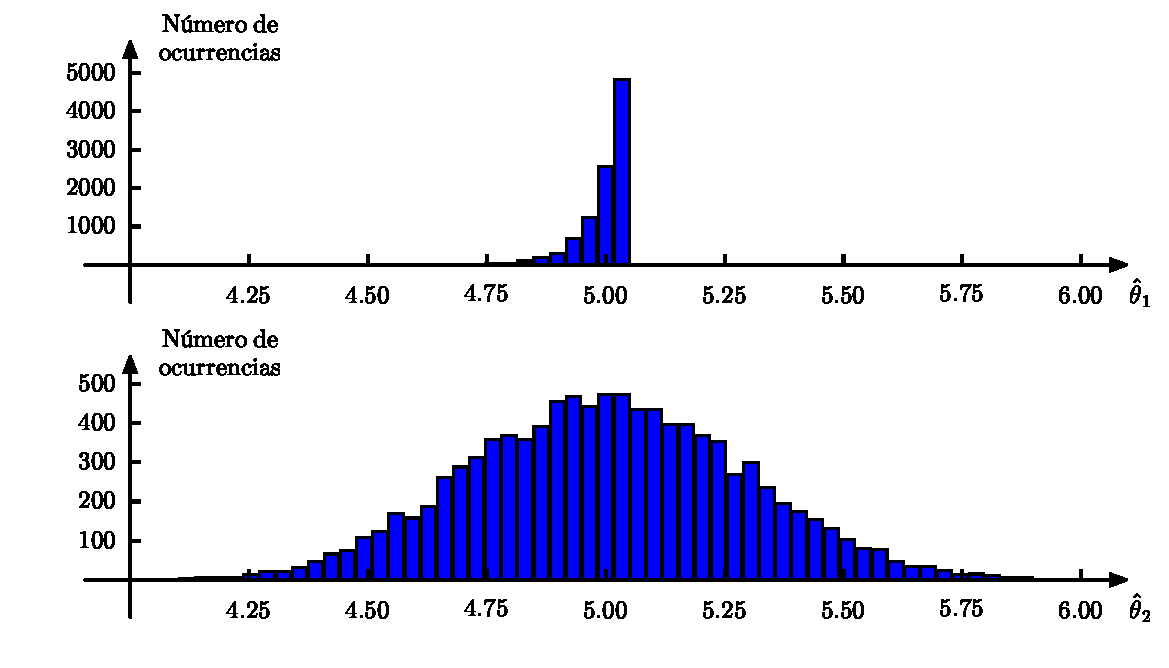
\includegraphics[width=\textwidth]{figuras/example_5_8.pdf}
\caption{\label{fig:example_5_8} Histogramas de los estimadores \(\hat{\theta}_1=(N+1)\max x[n]/(2N)\) y la media muestral \(\hat{\theta}_2\). Se calculó la media de \(N=100\) muestras de ruido uniforme \(\mathcal{U}(0,\,10)\) empleando ambos estimadores 10000 veces. Se observa que la dispersión de la media muestral respecto a la media \(\beta/2=5\) es mucho mayor.}
\end{center}
\end{figure}


Falta verificar que el estadístico \(T=\max x[n]\) es completo. Para hacerlo, se demostrará que dada una función \(g(\xi)\), si se cumple que \(E[g(T)]=0\) para todo valor del parámetro, necesariamente \(g(\xi)=0\) para todo \(\xi\) (esta demostración está basada en el ejemplo 6.2.23 en \cite{casella01statistical}). Efectivamente, considérese la función \(g(\xi)\) tal que
\[
 E[g(T)]=\int_{-\infty}^{\infty}g(\xi)p_T(\xi;\,\beta)d\xi=0,\qquad\forall\beta>0.
\]
Como \(E[g(T)]\) es la función nula, y por lo tanto constante para todo \(\beta\) se cumple que
\[
 \frac{d}{d\beta}E[g(T)]=0.
\]
Además,
\begin{align*}
 \frac{d}{d\beta}E[g(T)]&=\frac{d}{d\beta}\int_{-\infty}^{\infty}g(\xi)p_T(\xi;\,\beta)\,d\xi=0\\
  &\overset{(a)}{=}\frac{d}{d\beta}\int_{0}^{\beta}g(\xi)N\frac{\xi^{N-1}}{\beta^N}\,d\xi\\
  &=\frac{d}{d\beta}\left[\frac{1}{\beta^N}\int_{0}^{\beta}g(\xi)N\xi^{N-1}\,d\xi\right]\\
  &\overset{(b)}{=}\left(\frac{d}{d\beta}\frac{1}{\beta^N}\right)\int_{0}^{\beta}g(\xi)N\xi^{N-1}\,d\xi+\frac{1}{\beta^N}\frac{d}{d\beta}\int_{0}^{\beta}g(\xi)N\xi^{N-1}\,d\xi\\
  &\overset{(c)}{=}-\frac{N}{\beta^{N+1}}\int_{0}^{\beta}g(\xi)N\xi^{N-1}\,d\xi+\frac{1}{\beta^N}g(\beta)N\beta^{N-1}\,d\xi\\
  &=-\frac{N}{\beta}\int_{0}^{\beta}g(\xi)N\frac{\xi^{N-1}}{\beta^N}\,d\xi+\frac{N}{\beta}g(\beta)\\
  &\overset{(d)}{=}-\frac{N}{\beta}E[g(T)]+\frac{N}{\beta}g(\beta)\\
  &\overset{(e)}{=}\frac{N}{\beta}g(\beta),
\end{align*}
donde en \((a)\) se sustituyó la PDF de \(T\) dada por la ecuación \ref{eq:uniform_order_statistic_pdf}, en \((b)\) se empleó la regla de derivación de un producto, en \((c)\) se empleó el teorema fundamental del cálculo para determinar la derivada del segundo sumando\footnote{Ver \url{https://en.wikipedia.org/wiki/Fundamental_theorem_of_calculus} por ejemplo.}, en \((d)\) se notó que la integral es \(E[g(T)]\) y en \(e\) que \(E[g(T)]=0\).
Como
\[
 \frac{d}{d\beta}E[g(T)]=0=\frac{N}{\beta}g(\beta),\qquad\forall\beta>0,
\]
se concluye que \(g(\beta)=0\) para todo \(\beta>0\), y por lo tanto, el estadístico \(T\) es completo.

\section{Extensión a un parámetro vectorial}

En lo que sigue, se extienden los resultados en la búsqueda del estimador MVU en el caso en que el parámetro es un vector \(p\times 1\). La cantidad de estadísticos suficientes puede ser mayor que el número de parámetros (\(r>p\)), la misma cantidad (\(r=p\)) o incluso menor que el número de parámetros (\(r<p\)). La situación deseable es que el número de estadísticos suficientes sea igual al número de parámetros. De esta forma, podría buscarse una transformación del estadístico suficiente que lo haga insesgado.

\paragraph{Definición} Un vector estadístico \(\T(\x)=[T_1(\x)\,T_2(\x)\,\dots\, T_r(\x)]^T\) se dice suficiente para la estimación del parámetro \(\thetabf\) si la PDF de los datos condicionada al estadísitco \(p(\x\,|\,\T(\x);\,\thetabf)\) no depende de \(\thetabf\), es decir, \(p(\x\,|\,\T(\x);\,\thetabf)=p(\x\,|\,\T(\x))\). En general, existen muchos vectores \(\T(\x)\) que cumplen dicha condición, pero es de interés el \emph{estadístico suficiente mínimo}, que es el de menor dimensión.

\subsection{Teorema: Factorización de Neyman-Fisher (parámetro vectorial)}

Si la PDF \(p(\x;\,\thetabf)\) de los datos puede ser factorizada como
\begin{equation}\label{eq:general_mvu_neyman_fisher_factorization_vector}
 p(\x;\,\thetabf)=g(\T(\x),\,\thetabf)h(\x),
\end{equation}
donde \(g\) es una función que depende de \(\x\) solo a través de \(\T(\x)\), un estadístico \(r\times1\), y también de \(\thetabf\), y \(h\) es una función que depende solo de \(\x\), se cumple que \(\T(\x)\) es un estadístico suficiente de \(\thetabf\). Recíprocamente, si \(\T(\x)\) es un estadístico suficiente de \(\thetabf\), la PDF puede ser factorizada como la ecuación \ref{eq:general_mvu_neyman_fisher_factorization_vector}.

\subsection{Ejemplo: estimación de los parámetros de una sinusoide}\label{sec:general_mvu_sinusoidal_parameters_statistic}

Se considera el caso de una sinusoide en WGN,
\[
 x[n]=A\cos2\pi f_0 n+w[n],\qquad n=0,\,\dots,\,N-1,
\]
donde la amplitud \(A\), la frecuencia \(f_0\) y la varianza \(\sigma^2\) del ruido son desconocidas. El parámetro vectorial desconocido es entonces \(\thetabf=[A\,f_0\,\sigma^2]^T\). La PDF es
\[
 p(\x,\,\thetabf)=\frac{1}{(2\pi\sigma^2)^\frac{N}{2}}\exp\left[-\frac{1}{2\sigma^2}\sum_{n=0}^{N-1}(x[n]-A\cos2\pi f_0n)^2\right].
\]
Expandiendo el exponente, se tiene que
\[
 \sum_{n=0}^{N-1}(x[n]-A\cos2\pi f_0n)^2=\sum_{n=0}^{N-1}x^2[n]-2A\sum_{n=0}^{N-1}x[n]\cos2\pi f_0n+A^2\sum_{n=0}^{N-1}\cos^22\pi f_0n.
\]
Como la sumatoria del segundo sumando  depende tanto de los datos \(\x\) como del parámetro desconocido \(f_0\), la PDF no puede factorizarse como la ecuación \ref{eq:general_mvu_neyman_fisher_factorization_vector}. Sin embargo, si la frecuencia \(f_0\) fuera conocida y el parámetro desconocido fuera \(\thetabf=[A\,\sigma^2]^T\), la PDF se puede factorizar como
\[
 p(\x,\,\thetabf)=\underbrace{\frac{1}{(2\pi\sigma^2)^\frac{N}{2}}\exp\left[-\frac{1}{2\sigma^2}\left(\sum_{n=0}^{N-1}x^2[n]-2A\sum_{n=0}^{N-1}x[n]\cos2\pi f_0n+A^2\sum_{n=0}^{N-1}\cos^22\pi f_0n\right)\right]}_{\displaystyle g(T(\x),\,\theta)}\times\underbrace{\vphantom{\frac{1}{(2\pi\sigma^2)^\frac{N}{2}}\exp\left[-\frac{1}{2\sigma^2}\left(\sum_{n=0}^{N-1}x^2[n]-2A\sum_{n=0}^{N-1}x[n]\cos2\pi f_0n+A^2\sum_{n=0}^{N-1}\cos^22\pi f_0n\right)\right]} 1}_{\displaystyle h(\x)},
\]
donde 
\[
 \T(\x)=
 \begin{bmatrix}
  \displaystyle\sum_{n=0}^{N-1}x[n]\cos^22\pi f_0n\\
  \displaystyle\sum_{n=0}^{N-1}x^2[n]
 \end{bmatrix}.
\]
Por lo tanto, \(\T(\x)\) es un estadístico suficiente para \(A\) y \(\sigma^2\), pero solo en el caso en que la frecuencia \(f_0\) es conocida.

\subsection{Ejemplo: Nivel de DC en WGN con potencia del ruido desconocida}

Sea
\[
 x[n]=A+w[n],\qquad n=0,\,\dots,\,N-1,
\]
donde la amplitud \(A\) y la varianza \(\sigma^2\) del ruido son desconocidas. Observando que se trata del caso de la sinusoide en WGN del ejemplo anterior con \(f_0=0\), se tiene que el estadístico suficiente para el parámetro \(\thetabf=[A\,\sigma^2]^T\) es
\[
 \T(\x)=
 \begin{bmatrix}
  \displaystyle\sum_{n=0}^{N-1}x[n]\\
  \displaystyle\sum_{n=0}^{N-1}x^2[n]
 \end{bmatrix}.
\]
En el ejemplo de la sección \ref{sec:general_mvu_dc_in_wgn_sufficient}, se encontró que \(\sum_{n=0}^{N-1}x[n]\) es un estadístico suficiente de \(A\) cuando \(\sigma^2\) es conocido. También puede verse que \(\sum_{n=0}^{N-1}x^2[n]\) es un estadístico suficiente de \(\sigma^2\) cuando \(A\) es conocido. Esto sin embargo, no siempre se cumple. Como se encontró dos estadísticos suficientes para estimar dos parámetros, se debería poder encontrar un estimador MVU en este ejemplo.

\subsection{Teorema: Rao-Blackwell-Lehmann-Scheffe (parámetro vectorial)}

Si \(\check{\thetabf}\) es un estimador insesgado de \(\thetabf\) y \(\T(\thetabf)\) es un estadístico suficiente \(r\times1\) para \(\thetabf\), se cumple que \(\hat{\thetabf}=E(\check{\thetabf}\,|\,\T(\x))\) es
\begin{enumerate}
 \item un estimador válido de \(\thetabf\), en el sentido de que no depende de \(\thetabf\).
 \item insesgado
 \item de menor varianza que \(\check{\thetabf}\), para todo \(\thetabf\)
\end{enumerate}
Además, si el estadístico es completo, \(\hat{\thetabf}\) es el estimador MVU. En el caso vectorial, completitud significa que para una función \(r\times1\) arbitraria  \({\bf v}(\T)\) de \(\T\), si se cumple que
\[
 E({\bf v}(\T))=\int {\bf v}(\T)p(\T;\,\thetabf)\,d\T=\mathbf{0},\qquad\forall\,\thetabf
\]
se debe cumplir que
\[
 {\bf v}(\T)=\mathbf{0}\qquad\forall\,\T.
\]
En general, el cálculo de \(E(\check{\thetabf}\,|\,\T(\x))\) es difícil. Para poder determinar el estimador MVU sin tener que evaluar \(E(\check{\thetabf}\,|\,\T(\x))\), la dimensión del estadístico suficiente debe ser igual a la dimensión del parámetro desconocido, es decir, se debe cumplir que \(r=p\). En ese caso, solo se necesita encontrar una función \({\bf g}\) de dimensión \(p\) tal que
\[
 E({\bf g}(\T))=\thetabf
\]
donde \(\T\) es el estadístico suficiente.

\subsection{Ejemplo: Nivel de DC en WGN con potencia del ruido desconocida (continuación)}\label{sec:general_mvu_dc_in_wgn_unknown_power_mvu}

En este problema se encontró que el estadístico suficiente es
\[
 \T(\x)=
 \begin{bmatrix}
  T_1(\x)\\
  T_2(\x)
 \end{bmatrix}=
 \begin{bmatrix}
  \displaystyle\sum_{n=0}^{N-1}x[n]\\
  \displaystyle\sum_{n=0}^{N-1}x^2[n]
 \end{bmatrix}.
\]
Se intentará encontrar una función \({\bf g}\) que cumpla que \(E({\bf g}(\T))=\thetabf\). En el caso de encontrarla, \(\hat{\thetabf}={\bf g}(\T)\) es el estimador MVU. Para hacerlo, se parte calculando la media del estadístico  suficiente,
\[
 E(\T(\x))=
 \begin{bmatrix}
  NA\\
  NE(x^2[n])
 \end{bmatrix}=
 \begin{bmatrix}
  NA\\
  N(\sigma^2+A^2)
 \end{bmatrix}.
\]
Teniendo esto en cuenta, una transformación razonable es
\[
 {\bf g}(\T(\x))=
 \begin{bmatrix}
  \displaystyle\frac{1}{N}T_1(\x)\\
  \displaystyle\frac{1}{N}T_2(\x)-\left[\frac{1}{N}T_1(\x)\right]^2
 \end{bmatrix}=
 \begin{bmatrix}
  \bar{x}\\
  \displaystyle\frac{1}{N}\sum_{n=0}^{N-1}x^2[n]-\bar{x}^2
 \end{bmatrix}.
\]
Claramente, el sesgo del primer componente se elimina  dividiendo entre \(N\). Por otro lado, al dividir entre \(N\) el segundo componente se obtiene un estimador del segundo momento, \(E(x^2[n])=\sigma^2+A^2\), por lo que hay que restar una estimación de la media al cuadrado. De esta forma, se tiene que la esperanza del primer componente del estadístico transformado es
\[
 E(\bar{x})=A,
\]
y la del segundo componente es
\begin{align*}
 E\left(\frac{1}{N}\sum_{n=0}^{N-1}x^2[n]-\bar{x}^2\right)&=E(x^2[n])-E(\bar{x}^2)\\
  &\overset{(a)}{=}\left(\sigma^2+A^2\right)-\left(A^2+\frac{\sigma^2}{N}\right)\\
  &=\frac{N-1}{N}\sigma^2,
\end{align*}
donde en \((a)\) se consideró que \(\bar{x}\sim\mathcal{N}(A,\,\sigma^2/N)\) (ver el problema de la sección \ref{sec:problem_2_3}) y por lo tanto, \(E(\bar{x}^2)=A^2+\sigma^2/N\). El resultado indica que el segundo componente del estadístico transformado es sesgado, pero el sesgo se elimina multiplicando por \(N/(N-1)\). Finalmente, la transformación apropiada es
\[
 {\bf g}(\T(\x))=
 \begin{bmatrix}
  \displaystyle\frac{1}{N}T_1(\x)\\
  \displaystyle\frac{1}{N-1}\left\{T_2(\x)-N\left[\frac{1}{N}T_1(\x)\right]^2\right\}
 \end{bmatrix}=
 \begin{bmatrix}
  \bar{x}\\
  \displaystyle\frac{1}{N-1}\left(\sum_{n=0}^{N-1}x^2[n]-N\bar{x}^2\right)
 \end{bmatrix}.
\]
Notando que
\[
 \sum_{n=0}^{N-1}(x[n]-\bar{x})^2=\sum_{n=0}^{N-1}x^2[n]-2\bar{x}\sum_{n=0}^{N-1}x[n]+N\bar{x}^2
 =\sum_{n=0}^{N-1}x^2[n]-N\bar{x}^2,
\]
el estimador se puede escribir como
\[
 \hat{\thetabf}=
 \begin{bmatrix}
  \bar{x}\\
  \displaystyle\frac{1}{N-1}\sum_{n=0}^{N-1}(x[n]-\bar{x})^2
 \end{bmatrix},
\]
y es el estimador MVU para \(\thetabf=[A\,\sigma^2]\). En resumen, se obtuvo que cuando el parámetro desconocido es \(\thetabf=[A\,\sigma^2]\), el estimador MVU de la media es la media muestral \(\bar{x}\) y el estimador de la varianza es la \emph{varianza muestral} (\(\hat{\sigma^2}\)).
Se puede demostrar que las variables aleatorias \(\bar{x}\) y \(\hat{\sigma^2}\) son independientes (ver el ejemplo 8.20 de \cite{papoulis2002probability}) con PDF (ver sección la 7.2 de \cite{papoulis2002probability})
\begin{align*}
 \bar{x}&\sim\mathcal{N}\left(A,\,\frac{\sigma^2}{N}\right)\\
 \frac{(N-1)\hat{\sigma^2}}{\sigma^2}&\sim\chi^2_{N-1},
\end{align*}
Como la varianza de una variable aleatoria \(\chi^2_{k}\) es \(2k\), la varianza de \(\hat{\sigma^2}\) es
\[
 \var(\hat{\sigma^2})=\frac{\sigma^4}{(N-1)^2}\times2(N-1)=\frac{2\sigma^4}{N-1}.
\]
Se concluye que la matriz de covarianza del estimador es
\[
 \C_{\hat{\thetabf}}=
 \begin{bmatrix}
  \displaystyle\frac{\sigma^2}{N} & 0\\
  0 & \displaystyle\frac{2\sigma^4}{N-1}
 \end{bmatrix},
\]
y puede demostrarse que la CRLB es (ver el ejemplo 3.6 de \cite{kay93fundamentals})
\[
 \I^{-1}(\thetabf)=
 \begin{bmatrix}
  \displaystyle\frac{\sigma^2}{N} & 0\\
  0 & \displaystyle\frac{2\sigma^4}{N}
 \end{bmatrix}.
\]
Estos resultados muestran que el estimador MVU encontrado no alcanza la CRLB y por lo tanto, no es eficiente. Por esta misma razón, no podría haberse encontrado el estimador MVU mediante el estudio de la CRLB, es decir, intentando encontrar un estimador que alcance la cota.

\section{Problemas}

\subsection{Problema 1}

Se consideran los datos IID \(x[n]\sim\mathcal{N}(0,\,\sigma^2)\) con \(n=0,\,\dots,\,N-1\), y el parámetro desconocido es \(\sigma^2\). Probar que \(\sum_{n=0}^{N-1}x^2[n]\) es un estadístico suficiente de \(\sigma^2\) empleando la definición que indica que \(p(\x\,|\,\sum_{n=0}^{N-1}x^2[n]=T_0;\,\sigma^2)\) no depende de \(\sigma^2\). Sugerencia: Notar que la PDF de \(s=\sum_{n=0}^{N-1}x^2[n]/\sigma^2\) es chi-cuadrado con \(N\) grados de libertad (ver ecuaciones \ref{eq:pdf_chi_square} y \ref{eq:gamma_function}),
\[
\def\arraystretch{2.0}
 p(s)=
 \left\{\begin{array}{ll}
  \dfrac{s^{\frac{N}{2}-1}}{2^\frac{N}{2}\Gamma(N/2)}\exp\left(-\dfrac{s}{2}\right), & s\geq 0\\
  0, & s<0.
 \end{array} \right.
\]

\paragraph{Solución} Sea
\[
 T(\x)=\sum_{n=0}^{N-1}x^2[n],
\]
y se quiere probar que \(p(\x\,|\,T(\x)=T_0;\,\sigma^2)\) no depende de \(\sigma^2\).
Por el teorema de la probabilidad total, la probabilidad condicional es
\begin{equation}\label{eq:problem_5_1_cond_pdf}
 p(\x\,|\,T(\x)=T_0;\,\sigma^2)=\frac{p(\x,\,T(\x)=T_0;\,\sigma^2)}{p(T(\x)=T_0;\,\sigma^2)}.
\end{equation}
La probabilidad de los datos es
\[
 p(\x;\,\sigma^2)=\frac{1}{(2\pi\sigma^2)^\frac{N}{2}}\exp\left(-\frac{1}{2\sigma^2}\sum_{n=0}^{N-1}x^2[n]\right)
 =\frac{1}{(2\pi\sigma^2)^\frac{N}{2}}\exp\left[-\frac{T(\x)}{2\sigma^2}\right]
\]
por lo que la probabilidad conjunta es (ver la ecuación \ref{eq:general_mvu_statistic_join_pdf})
\begin{align}\label{eq:problem_5_1_joint_pdf}
 p(\x,\,T(\x)=T_0;\,\sigma^2)&=p(\x;\,\sigma^2)\delta(T(\x)-T_0)\nonumber\\
  &=\frac{1}{(2\pi\sigma^2)^\frac{N}{2}}\exp\left[-\frac{T(\x)}{2\sigma^2}\right]\delta(T(\x)-T_0).
\end{align}
Para  calcular \(p(T(\x)=T_0;\,\sigma^2)\), defínase la variable aleatoria 
\[
 s=\sum_{n=0}^{N-1}\frac{x^2[n]}{\sigma^2}.
\]
Como \(x[n]\sim\mathcal{N}(0,\,\sigma^2)\), \(x[n]/\sigma\sim\mathcal{N}(0,\,1)\), por lo que \(s\) es la suma del cuadrado \(N\) variables aleatorias IID con PDF \(\mathcal{N}(0,\,1)\), y puede demostrarse que tiene PDF chi-cuadrado con \(N\) grados de libertad (ver por ejemplo, el capítulo 7 de \cite{papoulis2002probability}), es decir, \(s\sim\chi^2(N)\) dada por la ecuación \ref{eq:pdf_chi_square}. Además,
\[
 T(\x)=\sum_{n=0}^{N-1}x^2[n]=\sigma^2s,
\]
y aplicando la ecuación \ref{eq:pdf_transformed_rv} de la PDF de una variable aleatoria transformada con \(g(s)=\sigma^2\) se tiene que
\begin{align}\label{eq:problem_5_1_statistic_pdf}
 p(T(\x);\,\sigma^2)&=\frac{1}{\sigma^2}p_s\left(\frac{T(\x)}{\sigma^2}\right)\nonumber\\
  &\overset{(a)}{=}\frac{\left[\dfrac{T(\x)}{\sigma^2}\right]^{\frac{N}{2}-1}}{\sigma^22^\frac{N}{2}\Gamma(N/2)}\exp\left[-\dfrac{T(\x)}{2\sigma^2}\right]\nonumber\\
  &=\frac{\left[T(\x)\right]^{\frac{N}{2}-1}}{\sigma^2(\sigma^2)^{\frac{N}{2}-1}2^\frac{N}{2}\Gamma(N/2)}\exp\left[-\dfrac{T(\x)}{2\sigma^2}\right]\nonumber\\
  &=\frac{\left[T(\x)\right]^{\frac{N}{2}-1}}{(2\sigma^2)^\frac{N}{2}\Gamma(N/2)}\exp\left[-\dfrac{T(\x)}{2\sigma^2}\right],
\end{align}
donde en \((a)\) se sustituyó la ecuación de la PDF \(\chi^2(N)\) evaluada en \(s=T(\x)/\sigma^2\). Sustituyendo las ecuaciones \ref{eq:problem_5_1_joint_pdf} y \ref{eq:problem_5_1_statistic_pdf} en la ecuación \ref{eq:problem_5_1_cond_pdf} con \(T(\x)=T_0\), se obtiene que
\begin{align*}
 p(\x\,|\,T(\x)=T_0;\,\sigma^2)&=\dfrac{\dfrac{1}{(2\pi\sigma^2)^\frac{N}{2}}\exp\left[-\dfrac{T_0}{2\sigma^2}\right]\delta(T(\x)-T_0)}{\dfrac{T_0^{\frac{N}{2}-1}}{(2\sigma^2)^\frac{N}{2}\Gamma(N/2)}\exp\left[-\dfrac{T_0}{2\sigma^2}\right]}\\
  &=\frac{\Gamma(N/2)}{\pi^\frac{N}{2}T_0^{\frac{N}{2}-1}}\delta(T(\x)-T_0),
\end{align*}
que es independiente de \(\sigma^2\). Se concluye que como la probabilidad condicional es independiente de \(\sigma^2\), \(T(\x)=\sum_{n=0}^{N-1}x^2[n]\) es un estadístico suficiente de \(\sigma^2\).

\subsection{Problema 2}

Las observaciones IID \(x[n]\) con \(n=0,\dots,\,N-1\) tienen PDF Rayleigh
\[
\def\arraystretch{2.0}
 p(x[n],\,\sigma^2)=
 \left\{\begin{array}{ll}
  \dfrac{x[n]}{\sigma^2}\exp\left(-\dfrac{1}{2}\dfrac{x^2[n]}{\sigma^2}\right), & x[n]\geq 0\\
  0, & x[n]<0.
 \end{array} \right.
\]
Encontrar un estadístico suficiente para \(\sigma^2\).

\paragraph{Solución} La PDF de los datos es
\begin{align*}
 p(\x;\,\sigma^2)&=\prod_{n=0}^{N-1}\frac{x[n]}{\sigma^2}\exp\left(-\frac{1}{2}\frac{x^2[n]}{\sigma^2}\right)u(x[n])\\
   &=\underbrace{\frac{1}{\sigma^{2N}}\exp\left(-\frac{1}{2\sigma^2}\sum_{n=0}^{N-1}x^2[n]\right)}_{\displaystyle g(T(\x),\,\theta)}\underbrace{u(\min x[n])\prod_{n=0}^{N-1}x[n]}_{\displaystyle h(\x)},
\end{align*}
concluyendo que el estadístico suficiente es
\[
 T(\x)=\sum_{n=0}^{N-1}x^2[n].
\]

\subsection{Problema 3}

Las observaciones IID \(x[n]\) con \(n=0,\dots,\,N-1\) tienen PDF exponencial
\[
 p(x[n],\,\lambda)=
 \left\{\begin{array}{ll}
  \lambda\exp\left(-\lambda x[n]\right), & x[n]\geq 0\\
  0, & x[n]<0.
 \end{array} \right.
\]
Encontrar un estadístico suficiente para \(\lambda\).

\paragraph{Solución} La PDF de los datos es
\begin{align*}
 p(\x;\,\lambda)&=\prod_{n=0}^{N-1}\lambda\exp\left(-\lambda x[n]\right)u(x[n])\\
   &=\underbrace{\lambda^N\exp\left(-\lambda\sum_{n=0}^{N-1}x[n]\right)}_{\displaystyle g(T(\x),\,\theta)}\underbrace{u(\min x[n])\vphantom{\prod_{n=0}^{N-1}x[n]}}_{\displaystyle h(\x)},
\end{align*}
concluyendo que el estadístico suficiente es
\[
 T(\x)=\sum_{n=0}^{N-1}x[n].
\]

\subsection{Problema 4}

Las observaciones IID \(x[n]\) con \(n=0,\dots,\,N-1\) tienen PDF \(\mathcal{N}(\theta,\,\theta)\) con \(\theta>0\). Encontrar un estadístico suficiente para \(\theta\).

\paragraph{Solución} La PDF de una muestra es
\[
 p(x[n];\,\theta)=\frac{1}{\sqrt{2\pi\theta}}\exp\left[-\frac{(x[n]-\theta)^2}{2\theta}\right],
\]
por lo que la PDF de los datos es
\[
 p(\x,\,\theta)=\frac{1}{(2\pi\theta)^\frac{N}{2}}\exp\left[-\frac{1}{2\theta}\sum_{n=0}^{N-1}(x[n]-\theta)^2\right].
\]
Desarrollando el exponente como
\[
 \sum_{n=0}^{N-1}(x[n]-\theta)^2=\sum_{n=0}^{N-1}x^2[n]-2\theta\sum_{n=0}^{N-1}x[n]+N\theta^2
\]
la PDF se puede expresar como
\begin{align*}
 p(\x,\,\theta)&=\frac{1}{(2\pi\theta)^\frac{N}{2}}\exp\left(-\frac{1}{2\theta}\sum_{n=0}^{N-1}x^2[n]+\sum_{n=0}^{N-1}x[n]-\frac{N\theta}{2}\right)\\
  &=\underbrace{\frac{1}{(2\pi\theta)^\frac{N}{2}}\exp\left(-\frac{1}{2\theta}\sum_{n=0}^{N-1}x^2[n]-\frac{N\theta}{2}\right)}_{\displaystyle g(T(\x),\,\theta)}\underbrace{\exp\left(\sum_{n=0}^{N-1}x[n]\right)}_{\displaystyle h(\x)},
\end{align*}
concluyendo que el estadístico suficiente es
\[
 T(\x)=\sum_{n=0}^{N-1}x^2[n].
\]

\subsection{Problema 5}

Las observaciones IID \(x[n]\) con \(n=0,\dots,\,N-1\) tienen PDF \(\mathcal{U}[-\theta,\,\theta]\) con \(\theta>0\). Encontrar un estadístico suficiente para \(\theta\).

\paragraph{Solución} La PDF de una muestra es
\[
 p(x[n];\,\theta)=\frac{1}{2\theta}\left[u(x[n]+\theta)-u(x[n]-\theta)\right],
\]
por lo que la PDF de los datos es
\[
 p(x[n];\,\theta)=\frac{1}{(2\theta)^N}\prod_{n=0}^{N-1}\left[u(x[n]+\theta)-u(x[n]-\theta)\right].
\]
Este producto es nulo a menos que \(-\theta<x[n]<\theta\) para todo \(x[n]\), o equivalentemente, \(\max x[n]<\theta\) y \(\min x[n]>-\theta\), o equivalentemente, \(\max|x[n]|<\theta\). De esta forma, se obtiene que
\[
 p(\x,\,\theta)=\underbrace{\frac{1}{(2\theta)^N}u(\theta-\max|x[n]|)}_{\displaystyle g(T(\x),\,\theta)}\times\underbrace{\vphantom{\frac{1}{(2\theta)^N}}1}_{\displaystyle h(\x)},
\]
concluyendo que el estadístico suficiente es
\[
 T(\x)=\max|x[n]|.
\]

\subsection{Problema 6}

Si se observan las muestras \(x[n]=A+w[n]\) con \(n=0,\dots,\,N-1\), donde \(w[n]\) es WGN con varianza \(\sigma^2\). Encontrar el estimador MVU para \(\sigma^2\) asumiendo que \(A\) es conocido. Asúmase que el estadístico suficiente es completo.

\paragraph{Solución} La PDF de los datos es
\[
 p(\x,\,\sigma^2)=\underbrace{\frac{1}{(2\pi\sigma^2)^\frac{N}{2}}\exp\left[-\frac{1}{2\sigma^2}\sum_{n=0}^{N-1}(x[n]-A)^2\right]}_{\displaystyle g(T(\x),\,\sigma^2)}\times\underbrace{\vphantom{\sum_{n=0}^{N-1}1}1}_{\displaystyle h(\x)},
\]
por lo que un estadístico suficiente es
\[
 T(\x)=\sum_{n=0}^{N-1}(x[n]-A)^2.
\]
La media del estadístico es
\[
 E(T(\x))=\sum_{n=0}^{N-1}E[(x[n]-A)^2]=N\sigma^2,
\]
por lo que al dividir entre \(N\) se transforma el estadístico suficiente en insesgado. Se concluye que
\[
 \hat{\sigma^2}=\frac{1}{N}\sum_{n=0}^{N-1}(x[n]-A)^2,
\]
es el estimador MVU.


\subsection{Problema 7}

Se considera el problema de la estimación de la frecuencia de una sinusoide en WGN,
\[
 x[n]=\cos2\pi f_0n+w[n],\qquad n=0,\,\dots,\,N-1,
\]
donde \(w[n]\) es WGN con varianza \(\sigma^2\) conocida. Mostrar que no es posible encontrar un estadístico suficiente para la frecuencia \(f_0\). 

\paragraph{Solución} La PDF de los datos es (ver el ejemplo de la sección \ref{sec:general_mvu_sinusoidal_parameters_statistic})
\begin{align*}
 p(\x,\,\thetabf)&=\frac{1}{(2\pi\sigma^2)^\frac{N}{2}}\exp\left[-\frac{1}{2\sigma^2}\sum_{n=0}^{N-1}(x[n]-\cos2\pi f_0n)^2\right]\\
   &=\frac{1}{(2\pi\sigma^2)^\frac{N}{2}}\exp\left(\sum_{n=0}^{N-1}x^2[n]+2\sum_{n=0}^{N-1}x[n]\cos2\pi f_0n+\sum_{n=0}^{N-1}\cos^22\pi f_0n\right).
\end{align*}
Debido al término \(\sum_{n=0}^{N-1}x[n]\cos2\pi f_0n\), la PDF parece no poder ser factorizada como indica la ecuación \ref{eq:general_mvu_neyman_fisher_factorization}, ya que en dicho término no puede separarse los datos del parámetro. Dicho término no puede ser un estadístico porque depende del parámetro \(f_0\) a estimar.

\subsection{Problema 8}

Se considera el problema de la estimación de una constante amortiguada en WGN,
\[
 x[n]=r^n+w[n],\qquad n=0,\,\dots,\,N-1,
\]
donde \(w[n]\) es WGN con varianza \(\sigma^2\) conocida. Mostrar que no es posible encontrar un estadístico suficiente para la constante \(r\). 

\paragraph{Solución} La PDF de los datos es 
\begin{align*}
 p(\x,\,\thetabf)&=\frac{1}{(2\pi\sigma^2)^\frac{N}{2}}\exp\left[-\frac{1}{2\sigma^2}\sum_{n=0}^{N-1}(x[n]-r^n)^2\right]\\
   &=\frac{1}{(2\pi\sigma^2)^\frac{N}{2}}\exp\left(\sum_{n=0}^{N-1}x^2[n]+2\sum_{n=0}^{N-1}x[n]r^n+\sum_{n=0}^{N-1}r^{2n}\right).
\end{align*}
Al igual que en el problema anterior, en el término \(\sum_{n=0}^{N-1}x[n]r^n\) no puede separarse los datos del parámetro, y por lo tanto, la PDF no puede ser factorizada como indica la ecuación \ref{eq:general_mvu_neyman_fisher_factorization}.

\subsection{Problema 9}

Se asume que \(x[n]\) es el resultado de un ensayo Bernoulli (tirar una moneda) con
\begin{align*}
 \Pr\{x[n]=1\}&=\theta\\
 \Pr\{x[n]=0\}&=1-\theta
\end{align*}
y se realizan \(N\) observaciones IID. Asumiendo que el teorema de la factorización de Neyman-Fisher se cumple también para variables aleatorias discretas, encontrar un estadístico suficiente para \(\theta\). Luego, asumiendo completitud del estadístico, encontrar el estimador MVU de \(\theta\).

\paragraph{Solución} La PDF de una muestra es
\[
 \Pr\{x[n];\,\theta\}=\theta^{x[n]}(1-\theta)^{1-x[n]},
\]
por lo que la PDF de los datos es
\begin{align*}
 \Pr\{\x;\,\theta\}&=\prod_{n=0}^{N-1}\theta^{x[n]}(1-\theta)^{1-x[n]}\\
  &=\theta^{\sum_{n=0}^{N-1}x[n]}(1-\theta)^{\sum_{n=0}^{N-1}(1-x[n])}\\
  &=\underbrace{\theta^{\sum_{n=0}^{N-1}x[n]}(1-\theta)^{N-\sum_{n=0}^{N-1}x[n]}}_{\displaystyle g(T(\x),\,\theta)}\times\underbrace{1\vphantom{(1-\theta)^N}}_{\displaystyle h(\x)}.
\end{align*}
Se concluye que un estadístico suficiente es
\[
 T(\x)=\sum_{n=0}^{N-1}x[n].
\]
Observando que la esperanza del estadístico suficiente es
\[
 E[T(\x)]=\sum_{n=0}^{N-1}E(x[n])=NE(x[n])\overset{(a)}{=}N\theta,
\]
donde en \((a)\) se tuvo en cuenta que la esperanza de una muestra es \(E(x[n])=1\times\theta+0\times(1-\theta)=\theta\). Por lo tanto, si se divide el estadístico suficiente entre \(N\) se hace insesgado, y el estimador MVU es
\[
 \hat{\theta}=\frac{1}{N}\sum_{n=0}^{N-1}x[n]=\bar{x},
\]
que es la media muestral.

\subsection{Problema 10}

En el problema de la estimación de la fase de una sinusoide en WGN (ver el ejemplo de la sección \ref{sec:general_mvu_sinusoidal_phase_statistic}) se propone el siguiente estimador
\[
 \hat{\phi}=-\arctan\left[\frac{T_2(\x)}{T_1(\x)}\right].
\]
Mostrar que si la SNR es grande o \(\sigma^2\to0\), para lo cual
\begin{equation}\label{eq:general_mvu_sinusoidal_phase_statistics_approx}
 \begin{aligned}
  T_1(\x)&\approx\sum_{n=0}^{N-1}A\cos(2\pi f_0 n+\phi)\cos2\pi f_0n\\
  T_2(\x)&\approx\sum_{n=0}^{N-1}A\cos(2\pi f_0 n+\phi)\sin2\pi f_0n,
 \end{aligned}
\end{equation}
el estimador cumple que \(\hat{\phi}\approx\phi\). Emplear las aproximaciones que se consideren apropiadas. ¿Es el estimador propuesto el estimador MVU?

\paragraph{Solución} El modelo de los datos en este problema es
\[
 x[n]=A\cos(2\pi f_0 n+\phi)+w[n],\qquad n=0,\,\dots,\,N-1.
\]
En el caso en que la SNR es grande o \(\sigma^2\to0\), se puede despreciar el ruido, y por lo tanto,
\[
 x[n]\approx A\cos(2\pi f_0 n+\phi),\qquad n=0,\,\dots,\,N-1.
\]
Sustituyendo \(x[n]\) por este valor en los estadísticos conjuntamente suficientes de \(\phi\) dados por la ecuación \ref{eq:general_mvu_sinusoidal_phase_statistics}, se obtiene que se pueden aproximar como la ecuación \ref{eq:general_mvu_sinusoidal_phase_statistics_approx}.

Considerando las identidades trigonométricas
\begin{align*}
 2\cos \theta \cos \varphi &={\cos(\theta -\varphi )+\cos(\theta +\varphi )}\\
 2\cos \theta \sin \varphi &={\sin(\theta +\varphi )-\sin(\theta -\varphi )},
\end{align*}
se tiene que 
\begin{align*}
 \cos(2\pi f_0 n+\phi)\cos2\pi f_0n&=\frac{\cos\phi+\cos(4\pi f_0 n+\phi)}{2}\\
 \cos(2\pi f_0 n+\phi)\sin2\pi f_0n&=\frac{\sin(4\pi f_0 n+\phi)-\sin\phi}{2},
\end{align*}
por lo que la ecuación \ref{eq:general_mvu_sinusoidal_phase_statistics_approx} se puede escribir como
\begin{align*}
  T_1(\x)&\approx \frac{NA}{2}\cos\phi+\frac{A}{2}\sum_{n=0}^{N-1}\cos(4\pi f_0 n+\phi)\\
  T_2(\x)&\approx \frac{A}{2}\sum_{n=0}^{N-1}\sin(4\pi f_0 n+\phi)-\frac{NA}{2}\sin\phi.
\end{align*}
De esta forma, se tiene que
\begin{align*}
 \frac{T_2(\x)}{T_1(\x)}&\approx\frac{\displaystyle\sum_{n=0}^{N-1}\sin(4\pi f_0 n+\phi)-N\sin\phi}{N\cos\phi+\displaystyle\sum_{n=0}^{N-1}\cos(4\pi f_0 n+\phi)}\\
 &=\frac{\displaystyle\frac{1}{N}\sum_{n=0}^{N-1}\sin(4\pi f_0 n+\phi)-\sin\phi}{\cos\phi+\displaystyle\frac{1}{N}\sum_{n=0}^{N-1}\cos(4\pi f_0 n+\phi)}\\
 &\overset{(a)}{\approx} -\frac{\sin\phi}{\cos\phi}\\
 &=\tan(-\phi),
\end{align*}
donde en \((a)\) se empleó el resultado del problema de la sección \ref{sec:problem_3_7} para despreciar las sumatorias. Por lo tanto,
\[
 \hat{\phi}=-\arctan\left[\frac{T_2(\x)}{T_1(\x)}\right]
 \approx-\arctan\left[\tan(-\phi)\right]=\phi,
\]
que es lo que se quería demostrar.

El estimador no es MVU ya que ni siquiera es insesgado. Por un lado, se cumple que \(\hat{\phi}\approx\phi\) solo si \(\sigma^2\to0\). Además, si se pudiera asumir que 
\begin{align*}
  E[T_1(\x)]&=\frac{NA}{2}\cos\phi\\
  E[T_2(\x)]&=-\frac{NA}{2}\sin\phi,
\end{align*}
que solo es cierto a altas SNR, se observa que
\begin{align*}
 E\left(\hat{\phi}\right)&=E\left\{-\arctan\left[\frac{T_2(\x)}{T_1(\x)}\right]\right\}\\
  &\neq-\arctan\left\{\frac{E[T_2(\x)]}{E[T_1(\x)]}\right\}\\
  &=\phi.
\end{align*}

\subsection{Problema 11}

En el problema de la estimación del nivel de DC en WGN (ver el ejemplo de la sección \ref{sec:general_mvu_dc_in_wgn_sufficient}) se desea estimar \(\theta=2A+1\) en lugar de \(A\). Encontrar un estimador MVU para \(\theta\). ¿Y si se deseara encontrar el estimador MVU del parámetro \(\theta=A^3\)? Sugerencia: reparametrizar la PDF en términos de \(\theta\) y seguir el enfoque habitual.

\paragraph{Solución}

Se quiere calcular el estimador MVU de \(\theta=2A+1\). Para hacerlo, se buscará un estadístico suficiente de \(\theta\) y luego una función del estadístico que lo haga insesgado. La PDF de los datos es
\[
 p(\x;\,A)=\frac{1}{(2\pi\sigma^2)^\frac{N}{2}}\exp\left[-\frac{1}{2\sigma^2}\sum_{n=0}^{N-1}(x[n]-A)^2\right],
\]
y sustituyendo \(A=(\theta-1)/2\) se tiene que 
\[
 p(\x;\,\theta)=\frac{1}{(2\pi\sigma^2)^\frac{N}{2}}\exp\left[-\frac{1}{2\sigma^2}\sum_{n=0}^{N-1}\left(x[n]-\frac{\theta-1}{2}\right)^2\right].
\]
Observando que la sumatoria del exponente se puede desarrollar como
\[
 \sum_{n=0}^{N-1}\left(x[n]-\frac{\theta-1}{2}\right)^2
  =\sum_{n=0}^{N-1}x^2[n]-(\theta-1)\sum_{n=0}^{N-1}x[n]+\frac{N(\theta-1)^2}{4},
\]
la PDF puede ser factorizada como
\[
 p(\x;\,\theta)=\underbrace{\frac{1}{(2\pi\sigma^2)^\frac{N}{2}}\exp\left\{-\frac{1}{2\sigma^2}\left[\frac{N(\theta-1)^2}{4}-(\theta-1)\sum_{n=0}^{N-1}x[n]\right]\right\}}_{\displaystyle g(T(\x),\,\theta)}\underbrace{\exp\left[-\frac{1}{2\sigma^2}\sum_{n=0}^{N-1}x^2[n]\right]}_{\displaystyle h(\x)}.
\]
Por lo tanto, un estadístico suficiente para \(\theta\) es
\[
 T(\x)=\sum_{n=0}^{N-1}x[n].
\]
Como \(T(\x)\) es completo, falta que encontrar una función \(g\) tal que \(E[g(T(\x))]=\theta=2A+1\). Teniendo en cuenta que \(E(T(\x))=NA\), se considera la función \(g(x)=1+2x/N\). De esta forma,
\[
 \hat{\theta}=1+\frac{2}{N}\sum_{n=0}^{N-1}x[n].
\]
Como \(E(\hat{\theta})=2A+1\), \(\hat{\theta}\) es el estimador MVU. 

Se buscará ahora el estimador MVU de \(\theta=A^3\) siguiendo el mismo enfoque. Sustituyendo \(A=\theta^\frac{1}{3}\) en la PDF de los datos, se tiene que
\[
 p(\x;\,\theta)=\frac{1}{(2\pi\sigma^2)^\frac{N}{2}}\exp\left[-\frac{1}{2\sigma^2}\sum_{n=0}^{N-1}(x[n]-\theta^\frac{1}{3})^2\right],
\]
y desarrollando el exponente, se ve que la PDF se puede factorizar como
\[
 p(\x;\,\theta)=\underbrace{\frac{1}{(2\pi\sigma^2)^\frac{N}{2}}\exp\left[-\frac{1}{2\sigma^2}\left(\theta^\frac{2}{3}-2A\theta^\frac{1}{3}\sum_{n=0}^{N-1}x[n]\right)\right]}_{\displaystyle g(T(\x),\,\theta)}\underbrace{\exp\left[-\frac{1}{2\sigma^2}\sum_{n=0}^{N-1}x^2[n]\right]}_{\displaystyle h(\x)},
\]
por lo que \(T(\x)=\sum_{n=0}^{N-1}x[n]\) es un estadístico suficiente para \(\theta\). Para hacerlo insesgado hay que encontrar una función \(g\) tal que
\(E[g(T(\x))]=A^3\), o equivalentemente, una función \(h\) tal que \(E[h(\bar{x})]=A^3\), ya que \(\bar{x}\) también es un estadístico suficiente para \(\theta\). Para intentar deducir la función \(h\) se calculará \(E(\bar{x}^3)\). Teniendo en cuenta que el momento tercero de una variable aleatoria \(x\sim\mathcal{N}(\mu,\,\sigma^2)\) es \(E(x^3)=\mu^3+3\mu\sigma^2\) y que \(\bar{x}\sim\mathcal{N}(A,\,\sigma^2/N)\), se cumple que
\[
 E(\bar{x}^3)=A^3+3A\frac{\sigma^2}{N}.
\]
Esto indica que si se considerara a \(\bar{x}^3\) como estimador de \(A^3\), habría un sesgo de \(3A\sigma^2/N\). Esto motiva a considerar como función \(h\) a
\[
 h(x)=x^3-3x\frac{\sigma^2}{N}.
\]
De esta forma,
\[
 \hat{\theta}=h(\bar{x})=\bar{x}^3-3\bar{x}\frac{\sigma^2}{N},
\]
con
\[
 E(\hat{\theta})=E(\bar{x}^3)-3E(\bar{x})\frac{\sigma^2}{N}
  =\left(A^3+3A\frac{\sigma^2}{N}\right)-3A\frac{\sigma^2}{N}=A^3,
\]
concluyendo que la función \(h\) propuesta hace al estadístico suficiente \(\bar{x}\) insesgado y por lo tanto, \(\hat{\theta}\) es el estimador MVU.


\subsection{Problema 12}

Este problema examina la idea de que los estadísticos suficientes son únicos a menos de transformaciones uno a uno. Considérese el problema de la estimación del nivel de DC en WGN del ejemplo de la sección \ref{sec:general_mvu_dc_in_wgn_sufficient}  pero con los estadísticos suficientes 
\begin{align*}
 T_1(\x)&=\sum_{n=0}^{N-1}x[n]\\
 T_2(\x)&=\left(\sum_{n=0}^{N-1}x[n]\right)^3.
\end{align*}
Encontrar funciones \(g_1\) y \(g_2\) tales que se satisfaga la condición de insesgado, o 
\begin{align*}
 E[g_1(T_1(\x))]&=A\\
 E[g_2(T_2(\x))]&=A,
\end{align*}
haciendo que los estadísticos suficientes transformados sean los estimadores MVU. ¿Es la transformación de \(T_1\) a \(T_2\) uno a uno? ¿Qué pasaría si se considerara el estadístico \(T_3(\x)=(\sum_{n=0}^{N-1}x[n])^2\)? 

 
\paragraph{Solución} Puede verse que las funciones \(g_1\) y \(g_2\) que hacen a los estadísticos insesgados son
\[
 g_1(x)=\frac{x}{N},\qquad\qquad  g_2(x)=\frac{x^{1/3}}{N},
\]
y la transformación de \(T_1\) a \(T_2\) es uno a uno. En el caso del estadístico \(T_3(\x)\), la transformación de \(T_1\) a \(T_3\) no es uno a uno, ya que las secuencias \(x[n]\) y \(-x[n]\) para todo \(n=0,\,\dots,\,N-1\), producen valores distintos de \(T_1(\x)\) pero valores iguales de \(T_3(\x)\), y por lo tanto, \(T_3(\x)\) no es un estadístico suficiente. Se podría considerar la función \(g_3(x)=\sqrt{x}/N\) para intentar hacer a \(T_3(\x)\) insesgado, pero en ese caso,
\[
 E[g_3(T_3(\x))]=E\left[\frac{\sqrt{(N\bar{x})^2}}{N}\right]=E\left[|\bar{x}|\right])=
 \left\{\begin{array}{rl}
  A, & A\geq 0\\
  -A, & A<0
 \end{array} \right.
 \neq A \qquad\forall\,A.
\]


\subsection{Problema 13}\label{sec:problem_5_13}

En este problema se deriva el estimador MVU para un ejemplo que no se ha trabajado previamente. Si se realizan \(N\) observaciones IID de acuerdo a la PDF
\[
 p(x[n];\,\theta)=
 \left\{\begin{array}{ll}
  \exp[-(x[n]-\theta)], & x[n]>\theta\\
  0, & x[n]<\theta,
 \end{array} \right.
\]
encontrar el estimador MVU de \(\theta\). Notar que \(\theta\) representa el mínimo valor que puede alcanzar \(x[n]\). Asumir que el estadístico suficiente es completo.

\paragraph{Solución} Para encontrar el estimador MVU, se buscará un estadístico suficiente de \(\theta\) y luego una transformación que lo haga insesgado. La PDF de una muestra se puede escribir como
\[
 p(x[n];\,\theta)=u(x[n]-\theta)\exp[-(x[n]-\theta)].
\]
Por lo tanto, la PDF de los datos es
\begin{align*}
 p(\x;\,\theta)&=\prod_{n=0}^{N-1}u(x[n]-\theta)\exp[-(x[n]-\theta)]\\
  &=u(\min x[n]-\theta)\exp\left[-\sum_{n=0}^{N-1}(x[n]-\theta)\right]\\
  &=u(\min x[n]-\theta)\exp\left(N\theta-\sum_{n=0}^{N-1}x[n]\right),
\end{align*}
que se puede factorizar como
\[
 p(\x;\,\theta)=\underbrace{u(\min x[n]-\theta)\exp\left(N\theta\right)\vphantom{\sum_{n=0}^{N-1}x[n]}}_{\displaystyle g(T(\x),\,\theta)}\underbrace{\exp\left(-\sum_{n=0}^{N-1}x[n]\right)}_{\displaystyle h(\x)},
\]
concluyendo que un estadístico suficiente de \(\theta\) es
\[
 T(\x)=\min x[n].
\]
Para buscar una transformación que lo haga insesgado, se procede de forma análoga al procedimiento del ejemplo de la sección \ref{sec:general_mvu_uniform_noise_mean}, el cual implica calcular la media de \(T=\min x[n]\), y por lo tanto, su densidad de probabilidad. La distribución de probabilidad de \(T\) es
\begin{align*}
 \Pr\{T\leq\xi\}&=1-\Pr\{T>\xi\}\\
  &=1-\Pr\{x[0]>\xi,\,x[1]>\xi,\,\dots,\,x[N-1]>\xi\}\\
  &=1-\Pr\{x[n]>\xi\}^N\\
  &=1-(1-\Pr\{x[n]\leq\xi\})^N,
\end{align*}
y derivando, se obtiene la densidad de probabilidad,
\begin{align}\label{eq:pdf_min_generic_va}
 p_T(\xi)&=\frac{d\Pr\{T\leq\xi\}}{d\xi}\nonumber\\
 &=-N(1-\Pr\{x[n]\leq\xi\})^{N-1}\left(-\frac{d\Pr\{x[n]\leq\xi\}}{d\xi}\right)\nonumber\\
   &=N(1-\Pr\{x[n]\leq\xi\})^{N-1}p_{x[n]}(\xi).
\end{align}
La distribución de probabilidad de \(x[n]\) se obtiene integrando la densidad de probabilidad, y para \(\xi>\theta\) es
\[
 \Pr\{x[n]\leq\xi\}=\int_{\infty}^{\xi}p_{x[n]}(u;\,\theta)\,du
  =\int_{\theta}^{\xi}e^{-(u-\theta)}\,du
  =-e^{-(u-\theta)}\bigg|_{\theta}^{\xi}
  =-\left[e^{-(\xi-\theta)}-1\right]
  =1-e^{-(\xi-\theta)},
\]
resultando en
\[
 \Pr\{x[n]\leq\xi\}=
 \left\{\begin{array}{ll}
  1-e^{-(\xi-\theta)}, & \xi>\theta\\
  0, & \xi<\theta.
 \end{array} \right.
\]
Sustituyendo el resultado en la ecuación de la densidad de probabilidad de \(T\) se tiene que para \(\xi>\theta\),
\[
 p_T(\xi)=N\{1-[1-e^{-(\xi-\theta)}]\}^{N-1}e^{-(\xi-\theta)}
   =Ne^{-(\xi-\theta)(N-1)}e^{-(\xi-\theta)}
   =Ne^{-N(\xi-\theta)},
\]
es decir,
\[
 p_T(\xi)=
 \left\{\begin{array}{ll}
  Ne^{-N(\xi-\theta)}, & \xi>\theta\\
  0, & \xi<\theta.
 \end{array} \right.
\]
Una vez obtenida la PDF de \(T\) es posible calcular su media,
\begin{align*}
 E(T)&=\int_{-\infty}^{\infty}\xi p_T(\xi)\,d\xi\\
  &=\int_{\theta}^{\infty}\xi Ne^{-N(\xi-\theta)}\,d\xi\\
  &\overset{(a)}{=}-\xi e^{-N(\xi-\theta)}\bigg|_{\theta}^{\infty} + \int_{\theta}^{\infty}e^{-N(\xi-\theta)}\,d\xi\\
  &=\theta + \left[-\frac{1}{N}e^{-N(\xi-\theta)}\bigg|_{\theta}^{\infty}\right]\\
  &=\theta+\frac{1}{N},
\end{align*}
donde en \((a)\) se aplicó integración por partes \(\int udv=uv-\int vdu\) con \(u=\xi\) y \(dv=Ne^{-N(\xi-\theta)}\) y por lo tanto, \(du=1\) y \(v=-e^{-N(\xi-\theta)}\). Se concluye que
\[
 E(\min x[n])=\theta+\frac{1}{N},
\]
obteniendo que
\[
 \hat{\theta}=\min x[n]-\frac{1}{N}
\]
es insesgado y por lo tanto, el estimador MVU.


\subsection{Problema 14}

Considérese una variable aleatoria \(x\) con PDF de la forma
\[
 p(x;\,\theta)=\exp[A(\theta)B(x)+C(x)+D(\theta)].
\]
Una PDF de este tipo se dice que pertenece a la \emph{familia exponencial escalar}\footnote{Ver \url{https://en.wikipedia.org/wiki/Exponential_family}} de PDF. Muchas propiedades útiles están asociadas a esta familia, y en particular, varias vinculadas a estadísticos suficientes, lo cual se explora en este problema y en el siguiente. Mostrar que las siguientes PDF pertenecen a dicha familia.
\begin{enumerate}[a.]
 \item Gaussiana
 \[
  p(x;\,\mu)=\frac{1}{\sqrt{2\pi}}\exp\left[-\frac{1}{2}(x-\mu)^2\right]
 \]
 \item Rayleigh
 \[
  p(x;\,\sigma^2)=
  \left\{\begin{array}{ll}
  \dfrac{x}{\sigma^2}\exp\left[-\dfrac{1}{2}\dfrac{x^2}{\sigma^2}\right], &  x>0\\
   0, &  x<0
 \end{array}\right.
 \]
 \item Exponencial
 \[
  p(x;\,\lambda)=
  \left\{\begin{array}{ll}
  \lambda\exp\left[-\lambda x\right], &  x>0\\
   0, &  x<0
 \end{array}\right.
 \]
 \item Laplace
 \[
  p(x;\,\sigma)=\frac{1}{\sqrt{2}\sigma}\exp\left[-\frac{\sqrt{2}|x-\mu|}{\sigma}\right]
 \]
\end{enumerate}

\paragraph{Solución} 

\begin{enumerate}[a.]
 \item Gaussiana
  \begin{align*}
    p(x;\,\mu)&=\frac{1}{\sqrt{2\pi}}\exp\left[-\frac{1}{2}(x-\mu)^2\right]\\
     &=\exp\left[\ln\left(\frac{1}{\sqrt{2\pi}}\right)\right]\exp\left[-\frac{1}{2}(x^2-2x\mu+\mu^2)\right]\\
     &=\exp\left[-\frac{1}{2}\ln2\pi\right]\exp\left[-\frac{1}{2}x^2+x\mu-\frac{1}{2}\mu^2\right],
  \end{align*}
  resultando en
  \[
   p(x;\,\mu)=\exp\left[\mu x-\frac{1}{2}x^2-\frac{1}{2}\left(\mu^2+\ln2\pi\right)\right],
  \]
  y por lo tanto, es de la familia exponencial con
  \[
   A(\mu)B(x)=\mu x, \qquad C(x)=-\frac{1}{2}x^2,\qquad D(\mu)=-\frac{1}{2}\left(\mu^2+\ln2\pi\right).
  \]
 \item Rayleigh
 \begin{align*}
  p(x;\,\sigma^2)&=u(x)\dfrac{x}{\sigma^2}\exp\left[-\dfrac{1}{2}\dfrac{x^2}{\sigma^2}\right]\\
   &=\exp\left[\ln xu(x)-\ln\sigma^2\right]\exp\left[-\dfrac{1}{2}\dfrac{x^2}{\sigma^2}\right],
 \end{align*}
 resultando en
 \[
  p(x;\,\sigma^2)=\exp\left[-\frac{1}{2}\frac{x^2}{\sigma^2}+\ln xu(x)-\ln\sigma^2\right]
 \]
 y por lo tanto, es de la familia exponencial con
  \[
   A(\sigma^2)B(x)=-\frac{1}{2}\frac{x^2}{\sigma^2}, \qquad C(x)=\ln xu(x),\qquad D(\sigma^2)=-\ln\sigma^2.
  \]
 \item Exponencial
 \begin{align*}
  p(x;\,\lambda)&=u(x)\lambda\exp\left[-\lambda x\right]\\
   &=\exp\left[\ln u(x)+\ln\lambda\right]\exp\left[-\lambda x\right],
 \end{align*}
 resultando en
 \[
  p(x;\,\lambda)=\exp\left[-\lambda x+\ln u(x)+\ln\lambda\right],
 \]
 y por lo tanto, es de la familia exponencial con
  \[
   A(\lambda)B(x)=-\lambda x, \qquad C(x)=\ln u(x),\qquad D(\lambda)=\ln\lambda.
  \]
 \item Laplace
 \begin{align*}
   p(x;\,\sigma)&=\frac{1}{\sqrt{2}\sigma}\exp\left[-\frac{\sqrt{2}|x-\mu|}{\sigma}\right]\\
    &=\exp[\ln\sqrt{2}\sigma]\exp\left[-\frac{\sqrt{2}|x-\mu|}{\sigma}\right]
 \end{align*}
resultando en 
\[
 p(x;\,\sigma)=\exp\left[\ln\sqrt{2}\sigma-\frac{\sqrt{2}|x-\mu|}{\sigma}\right]
\]
y por lo tanto, es de la familia exponencial con
  \[
   A(\sigma)B(x)=\frac{\sqrt{2}}{\sigma}|x-\mu|, \qquad C(x)=0,\qquad D(\sigma)=\ln\sqrt{2}\sigma.
  \]
\end{enumerate}

\subsection{Problema 15}\label{sec:problem_5_15}

Si se observan las muestras \(x[n]\) para \(n=0,\,\dots,\,N-1\), las cuales son IID con PDF de la familia exponencial, mostrar que
\[
 T(\x)=\sum_{n=0}^{N-1}B(x[n])
\]
es un estadístico suficiente ara \(\theta\). Luego, aplicar este resultado para determinar un estadístico suficiente para las PDF Gaussiana, Rayleigh, exponencial y Laplace del problema anterior. Finalmente, asumiendo que los estadísticos suficientes son completos, encontrar un estimador en cada caso si es posible.

\paragraph{Solución} La PDF de cada muestra \(x[n]\) pertenece a la familia de PDFs exponenciales, y por lo tanto es de la forma
\[
 p(x[n];\,\theta)=\exp[A(\theta)B(x[n])+C(x[n])+D(\theta)].
\]
Como las muestras son IID, la PDF de los datos es
\begin{align*}
 p(x[n];\,\theta)&=\prod_{n=0}^{N-1}\exp[A(\theta)B(x[n])+C(x[n])+D(\theta)]\\
  &=\exp\left\{\sum_{n=0}^{N-1}\left[A(\theta)B(x[n])+C(x[n])+D(\theta)\right]\right\}\\
  &=\exp\left[A(\theta)\sum_{n=0}^{N-1}B(x[n])+\sum_{n=0}^{N-1}C(x[n])+ND(\theta)\right],
\end{align*}
que puede factorizarse como
\[
 p(x[n];\,\theta)=\underbrace{\exp\left[A(\theta)\sum_{n=0}^{N-1}B(x[n])+ND(\theta)\right]}_{\displaystyle g(T(\x),\,\theta)}\underbrace{\exp\left[\sum_{n=0}^{N-1}C(x[n])\right]}_{\displaystyle h(\x)},
\]
y por lo tanto,
\[
 T(\x)=\sum_{n=0}^{N-1}B(x[n])
\]
es un estadístico suficiente para \(\theta\). A partir de este resultado y empleando el resultado del problema anterior se tiene que los estadísticos suficientes son
\begin{enumerate}[a.]
 \item Gaussiana
  \[
   T(\x)=\sum_{n=0}^{N-1}x[n]
  \]
 \item Rayleigh
 \[
   T(\x)=\sum_{n=0}^{N-1}x^2[n]
 \]
 \item Exponencial
  \[
   T(\x)=\sum_{n=0}^{N-1}x[n]
  \]
 \item Laplace 
 \[
   T(\x)=\sum_{n=0}^{N-1}|x[n]-\mu|
 \]
\end{enumerate}
Se buscará a partir del estadístico suficiente el estimador MVU en cada caso.
\begin{enumerate}[a.]
\item Gaussiana
  \[
   \hat{\mu}=\frac{1}{N}\sum_{n=0}^{N-1}x[n],
  \]
  como ya se vió previamente.
 \item Rayleigh. La esperanza del estadístico suficiente es
 \[
   E[T(\x)]=NE(x^2[n]).
 \]
 Para completar el resultado, hay que calcular el segundo momento,
 \begin{align*}
  E(x^2)&=\int_{-\infty}^{\infty}x^2p(x;\,\sigma^2)\,dx\\
   &=\frac{1}{\sigma^2}\int_{0}^{\infty}x^3e^{-x^2/2\sigma^2}\,dx\\
   &\overset{(a)}{=}\frac{1}{2\sigma^2}\int_{0}^{\infty}ye^{-y/2\sigma^2}\,dy\\
   &\overset{(b)}{=}-ye^{-y/2\sigma^2}\bigg|_{0}^\infty+\int_{0}^{\infty}e^{-y/2\sigma^2}\,dy\\
   &=-2\sigma^2e^{-y/2\sigma^2}\bigg|_{0}^{\infty}\\
   &=2\sigma^2,
 \end{align*}
donde en \((a)\) se realizó el cambio de variable \(y=x^2\), \(dy=2xdx\), y en \((b)\) se aplicó integración por partes \(\int udv=uv-\int vdu\) con \(u=y\) y \(dv=(1/2\sigma^2)e^{-y/2\sigma^2}\) y por lo tanto, \(du=1\) y \(v=-e^{-y/2\sigma^2}\). Sustituyendo este resultado en la esperanza del estadístico suficiente se obtiene que
\[
 E[T(\x)]=NE(x^2[n])=2N\sigma^2,
\]
y por lo tanto, el estimador MVU de \(\sigma^2\) es
\[
 \hat{\sigma^2}=\frac{1}{2N}\sum_{n=0}^{N-1}x^2[n].
\]
 \item Exponencial. La esperanza del estadístico es
 \[
  E[T(\x)]=NE(x[n]),
 \]
 con 
 \begin{align*}
  E(x)&=\int_{0}^{\infty}x\lambda e^{-\lambda x}\,dx\\
   &\overset{(a)}{=}-xe^{-\lambda x}\bigg|_{0}^{\infty}+\int_{0}^{\infty}e^{-\lambda x}\,dx\\
   &=-\frac{1}{\lambda}e^{-\lambda x}\bigg|_{0}^{\infty}\\
   &=\frac{1}{\lambda},
 \end{align*}
donde en \((a)\) se aplicó integración por partes \(\int udv=uv-\int vdu\) con \(u=x\) y \(dv=\lambda e^{-\lambda x}\) y por lo tanto, \(du=1\) y \(v=-e^{-\lambda x}\). De esta forma, se tiene que
\[
 E[T(\x)]=NE(x[n])=\frac{N}{\lambda}.
\]
En este caso, no parece evidente una transformación del estadístico que lo haga insesgado. Se podría pensar en
\[
 \hat{\lambda}=\frac{N}{T(\x)},
\]
pero
\[
 E[\hat{\lambda}]=E\left[\frac{N}{T(\x)}\right]\neq \frac{N}{E\left[T(\x)\right]}=\lambda.
\]
Sin embargo, si se reparametriza la PDF con \(\theta=1/\lambda\), se tiene que
\[
 p(x[n])=\frac{u(x[n])}{\theta}e^{-x[n]/\theta}
\]
y
\[
 p(\x,\,\theta)=\underbrace{\frac{1}{\theta^N}\exp\left(-\frac{1}{\theta}\sum_{n=0}^{N-1}x[n]\right)}_{\displaystyle g(T(\x),\,\theta)}\underbrace{u(\min x[n])\vphantom{\sum_{n=0}^{N-1}x[n]}}_{\displaystyle h(\x)},
\]
por lo que un estadístico de \(\theta\) es
\[
 T(\x)=\sum_{n=0}^{N-1}x[n].
\]
y 
\[
 E[T(\x)]=\frac{N}{\lambda}=N\theta
\]
y por lo tanto,
\[
 \hat{\theta}=\frac{1}{N}\sum_{n=0}^{N-1}x[n]
\]
es el estimador MVU de \(\theta\).
\item Laplace. La esperanza del estadístico es
\[
 E[T(\x)]=NE(|x[n]-\mu|)
\]
con 
\begin{align*}
 E(|u-\mu|)&=\int_{-\infty}^{\infty}|u-\mu|\frac{1}{\sqrt{2}\sigma}e^{-\sqrt{2}|u-\mu|/\sigma}\,du\\
  &\overset{(a)}{=}\frac{1}{\sqrt{2}\sigma}\int_{-\infty}^{\infty}|x|e^{-\sqrt{2}|x|/\sigma}\,dx\\
  &\overset{(b)}{=}\frac{\sqrt{2}}{\sigma}\int_{0}^{\infty}xe^{-\sqrt{2}x/\sigma}\,dx\\
  &\overset{(c)}{=}-xe^{-\sqrt{2}x/\sigma}\bigg|_{0}^{\infty}+\int_{0}^{\infty}e^{-\sqrt{2}x/\sigma}\,dx\\
  &=-\frac{\sigma}{\sqrt{2}}e^{-\sqrt{2}x/\sigma}\bigg|_{0}^{\infty}\\
  &=\frac{\sigma}{\sqrt{2}},
\end{align*}
donde en \((a)\) se realizó el cambio de variable \(x=u-\mu\), en \((b)\) se tuvo en cuenta que el integrando es una función par y en \((c)\) se aplicó integración por partes \(\int udv=uv-\int vdu\) con \(u=x\) y \(dv=(\sqrt{2}/\sigma)e^{-\sqrt{2}x/\sigma}dx\) y por lo tanto, \(du=dx\) y \(v=-e^{-\sqrt{2}x/\sigma}\). Por lo tanto,
\[
 E[T(\x)]=N\frac{\sigma}{\sqrt{2}},
\]
resultando en que
\[
 \hat{\sigma}=\frac{\sqrt{2}}{N}\sum_{n=0}^{N-1}|x[n]-\mu|
\]
es el estimador MVU.
\end{enumerate}


\subsection{Problema 16}

En este problema se da un ejemplo donde la cantidad de estadísticos suficientes es menor que el número de parámetros a estimar. Asúmase que se observa \(x[n]\) para \(n=0,\,\dots,\,N-1\) con \(\x\sim\mathcal{N}(\mubf,\,\C)\) con
\[
 \mubf=
 \begin{bmatrix}
  N\mu\\
  0\\
  0\\
  \vdots\\
  0\\
 \end{bmatrix}
 \qquad\qquad\textrm{y}\qquad\qquad
 \C=
 \begin{bmatrix}
  N-1+\sigma^2 & -\mathbf{1}^T\\
  -\mathbf{1} & \I
 \end{bmatrix}.
\]
La matriz \(\C\) de covarianza tiene dimensiones 
\[
 \begin{bmatrix}
  1\times1 & 1\times (N-1)\\
  (N-1) \times1 & (N-1)\times(N-1)
 \end{bmatrix}.
\]
Mostrar que con \(\thetabf=[\mu\,\sigma^2]\),
\[
 p(\x;\,\thetabf)=\frac{1}{(2\pi)^\frac{N}{2}\sigma}\exp\left\{-\frac{1}{2}\left[\frac{N^2}{\sigma^2}(\bar{x}-\mu)^2+\sum_{n=1}^{N-1}x^2[n]\right]\right\}.
\]
¿Cuales son los estadísticos suficientes para \(\thetabf\)? Sugerencia: se necesita encontrar la inversa y el determinante de una matriz en bloques y emplear la identidad de Woodbury.

\paragraph{Solución} La PDF de los datos es
\begin{equation}\label{eq:gaussian_multivariate_pdf}
 p(\x,\,\thetabf)=\frac{1}{(2\pi)^\frac{N}{2}\sqrt{\det(\C)}}\exp\left\{-\frac{1}{2}(\x-\mubf)^T\C^{-1}(\x-\mubf)\right\}.
\end{equation}
Para continuar el desarrollo es necesario calcular el determinante y la inversa de la matriz \(\C\) de covarianza. Como se indica en el apéndice \ref{ap:block_matrix_properties} el determinante de una matriz en bloques es (ecuación \ref{eq:block_matrix_determinant})
\[
 \det{\begin{bmatrix}
   \A & \B\\
   \C & \D
  \end{bmatrix}}
=\det(\D)\times \det \left(\A-\B\D^{-1}\C\right)
\]
(no confundir a \(\C\) con la matriz de covarianza en esta identidad). En el caso que se quiere resolver, \(\A=N-1+\sigma^2\), \(\B=-\mathbf{1}^T\), \(\C=-\mathbf{1}\) y \(\D=\I\) y por lo tanto,
\[
 \A-\B\D^{-1}\C=N-1+\sigma^2-\mathbf{1}^T\I\mathbf{1}=N-1+\sigma^2-\mathbf{1}^T\mathbf{1}=N-1+\sigma^2-(N-1)=\sigma^2,
\]
resultando en que el determinante de la matriz \(\C\) de covarianza es
\begin{equation}\label{eq:problem_5_16_determinant_tmp}
 \det(\C)=\det(\I)\times\det(\sigma^2)=\sigma^2.
\end{equation}
Para calcular la inversa de la matriz de covarianza se usa la ecuación \ref{eq:block_matrix_inverse} del apéndice \ref{ap:block_matrix_properties}, que indica que
\[
  {\begin{bmatrix}
 \A & \B \\
 \C & \D
 \end{bmatrix}}^{-1}
 =\begin{bmatrix}
 (\A- \B\D^{-1}\C)^{-1} & -(\A-\B\D^{-1}\C)^{-1}\B\D^{-1}\\
 -\D^{-1}\C(\A-\B\D^{-1}\C)^{-1} & \quad\D^{-1}+\D^{-1}\C(\A-\B\D^{-1}\C)^{-1}\B\D^{-1}
 \end{bmatrix}.
\]
En este caso se tiene que
\[
  \begin{array}{c}
    \displaystyle(\A- \B\D^{-1}\C)^{-1} = \frac{1}{\sigma^2},\qquad\qquad-(\A-\B\D^{-1}\C)^{-1}\B\D^{-1} =-\frac{1}{\sigma^2}\mathbf{1}^T\\
    \displaystyle-\D^{-1}\C(\A-\B\D^{-1}\C)^{-1}=-\frac{1}{\sigma^2}\mathbf{1},\qquad\qquad
    \D^{-1}+\D^{-1}\C(\A-\B\D^{-1}\C)^{-1}\B\D^{-1}=\I+\frac{1}{\sigma^2}\mathbf{1}\mathbf{1}^T,
  \end{array}
\]
resultando en que la matriz de covarianza inversa es
\[
 \C=\frac{1}{\sigma^2}
 \begin{bmatrix}
 1 & \mathbf{1}^T\\
 \mathbf{1} & \sigma^2\I+\mathbf{1}\mathbf{1}^T
 \end{bmatrix}.
\]
A continuación, se calculará la expresión del exponente de la PDF. Para eso, se observa que
\[
 \C(\x-\mubf)
 =\frac{1}{\sigma^2}
 \begin{bmatrix}
  1 & 1 & 1 & \dots & 1\\
  1 & \sigma^2+1 & 1 & \dots & 1\\
  \vdots & \ddots & \ddots & \ddots & \vdots \\
  \vdots & & \ddots & \ddots & 1\\
  1 & \dots & \dots &  1 & \sigma^2+1
 \end{bmatrix}
 \begin{bmatrix}
  x[0]-N\mu \\
  x[1]\\
  \vdots\\
  x[N-1]
 \end{bmatrix}=\frac{1}{\sigma^2}
 \begin{bmatrix}
  \displaystyle\sum_{n=0}^{N-1}x[n]-N\mu \\
  \displaystyle\sum_{n=0}^{N-1}x[n]+x[1]\sigma^2-N\mu\\
  \vdots\\
  \displaystyle\sum_{n=0}^{N-1}x[n]+x[N-1]\sigma^2-N\mu
 \end{bmatrix}.
\]
Luego,
\[
 (\x-\mubf)^T\C(\x-\mubf)=
 \begin{bmatrix}
  x[0]-N\mu & x[1] & \dots & x[N-1]
 \end{bmatrix}\frac{1}{\sigma^2}
 \begin{bmatrix}
  \displaystyle\sum_{n=0}^{N-1}x[n]-N\mu \\
  \displaystyle\sum_{n=0}^{N-1}x[n]+x[1]\sigma^2-N\mu\\
  \vdots\\
  \displaystyle\sum_{n=0}^{N-1}x[n]+x[N-1]\sigma^2-N\mu
 \end{bmatrix}
\]
resulta en
\begin{align*}
 (\x-\mubf)^T\C(\x-\mubf)&=\frac{1}{\sigma^2}\left[(x[0]-N\mu)\left(\sum_{n=0}^{N-1}x[n]-N\mu\right)
   +\sum_{m=1}^{N-1}x[m]\left(\sum_{n=0}^{N-1}x[n]+x[m]\sigma^2-N\mu\right)\right]\\
  &=\frac{1}{\sigma^2}\Bigg[x[0]\sum_{n=0}^{N-1}x[n]-N\mu x[0]-N\mu\sum_{n=0}^{N-1}x[n]+N^2\mu^2\\
  &\qquad+\sum_{m=1}^{N-1}x[m]\sum_{n=0}^{N-1}x[n]
   +\sigma^2\sum_{m=1}^{N-1}x^2[m]-N\mu\sum_{m=1}^{N-1}x[m]\Bigg]\\
  &\overset{(a)}{=}\frac{1}{\sigma^2}\left[-N\mu\sum_{n=0}^{N-1}x[n]+N^2\mu^2+\sum_{m=0}^{N-1}x[m]\sum_{n=0}^{N-1}x[n]+\sigma^2\sum_{m=1}^{N-1}x^2[m]-N\mu\sum_{m=0}^{N-1}x[m]\right]\\
  &=\frac{1}{\sigma^2}\left[N^2\mu^2-2N\mu\sum_{n=0}^{N-1}x[n]+\left(\sum_{n=0}^{N-1}x[n]\right)^2+\sigma^2\sum_{n=1}^{N-1}x^2[n]\right],
\end{align*}
donde en \((a)\) se agrupó en una única sumatoria el primer sumando con el quinto sumando y el segundo sumando con el último sumando. Luego, operando, se tiene que
\begin{align}\label{eq:problem_5_16_exponent_tmp}
 (\x-\mubf)^T\C(\x-\mubf)&=\left\{\frac{N^2}{\sigma^2}\left[\mu^2-2\mu\frac{1}{N}\sum_{n=0}^{N-1}x[n]+\left(\frac{1}{N}\sum_{n=0}^{N-1}x[n]\right)^2\right]+\sum_{n=1}^{N-1}x^2[n]\right\}\nonumber\\
  &=\left[\frac{N^2}{\sigma^2}\left(\mu^2-2\mu\bar{x}+\bar{x}^2\right)^2+\sum_{n=1}^{N-1}x^2[n]\right]\nonumber\\
  &=\left[\frac{N^2}{\sigma^2}\left(\mu-\bar{x}\right)^2+\sum_{n=1}^{N-1}x^2[n]\right].
\end{align}
Finalmente, sustituyendo las ecuaciones \ref{eq:problem_5_16_determinant_tmp} y \ref{eq:problem_5_16_exponent_tmp} en la ecuación \ref{eq:gaussian_multivariate_pdf}, se obtiene que la PDF de los datos se puede expresar como
\[
 p(\x,\,\thetabf)=\frac{1}{(2\pi)^\frac{N}{2}\sigma}\exp\left\{-\frac{1}{2}\left[\frac{N^2}{\sigma^2}\left(\mu-\bar{x}\right)^2+\sum_{n=1}^{N-1}x^2[n]\right]\right\},
\]
y observando que se puede factorizar como
\[
 p(\x,\,\thetabf)=\underbrace{\frac{1}{(2\pi)^\frac{N}{2}\sigma}\exp\left\{-\frac{N^2}{2\sigma^2}\left(\mu-\bar{x}\right)^2\right\}\vphantom{\sum_{n=1}^{N-1}}}_{\displaystyle g(T(\x),\,\thetabf)}\underbrace{\exp\left\{-\frac{1}{2}\sum_{n=1}^{N-1}x^2[n]\right\}}_{\displaystyle h(\x)},
\]
se concluye que \(T(\x)=\bar{x}\) es un estadístico suficiente de \(\thetabf=[\mu\,\sigma^2]^T\).

\subsection{Problema 17}

Se considera una sinusoide de frecuencia conocida en WGN, o
\[
 x[n]=A\cos2\pi f_0n+w[n],\qquad n=0,\,\dots,\,N-1,
\]
donde \(w[n]\) es WGN de varianza \(\sigma^2\). Encontrar el estimador MVU de
\begin{enumerate}[a.]
 \item la amplitud \(A\) asumiendo que \(\sigma^2\) es conocido
 \item la amplitud \(A\) y la varianza \(\sigma^2\) del ruido.
\end{enumerate}
Se puede asumir que el estadístico suficiente es completo. Sugerencia: los resultados de los ejemplos de las secciones \ref{sec:general_mvu_sinusoidal_parameters_statistic} y \ref{sec:general_mvu_dc_in_wgn_unknown_power_mvu} pueden ser útiles.

\paragraph{Solución} 
\begin{enumerate}[a.]
 \item Se considera el caso en que \(\sigma^2\) es conocido y se quiere calcular \(A\). Como se determinó en el ejemplo de la sección \ref{sec:general_mvu_sinusoidal_parameters_statistic}, la PDF de los datos es
\[
 p(\x,\,A)=\frac{1}{(2\pi\sigma^2)^\frac{N}{2}}\exp\left[-\frac{1}{2\sigma^2}\left(\sum_{n=0}^{N-1}x^2[n]-2A\sum_{n=0}^{N-1}x[n]\cos2\pi f_0n+A^2\sum_{n=0}^{N-1}\cos^22\pi f_0n\right)\right]
\]
y como en este caso \(\sigma^2\) es conocido, se puede factorizar como
\begin{align*}
 p(\x,\,A)&=\underbrace{\frac{1}{(2\pi\sigma^2)^\frac{N}{2}}\exp\left[-\frac{1}{2\sigma^2}\left(-2A\sum_{n=0}^{N-1}x[n]\cos2\pi f_0n+A^2\sum_{n=0}^{N-1}\cos^22\pi f_0n\right)\right]}_{\displaystyle g(T(\x),\,A)}\times\\
 &\qquad\underbrace{\exp\left[-\frac{1}{2\sigma^2}\sum_{n=0}^{N-1}x^2[n]\right]}_{\displaystyle h(\x)},
\end{align*}
concluyendo que el estadístico suficiente es
\[
 T(\x)=\sum_{n=0}^{N-1}x[n]\cos2\pi f_0n.
\]
El estimador MVU es una función del estadístico suficiente que lo haga insesgado. Para intentar encontrarla, se calcula la media del estadístico,
\begin{align*}
 E(T(\x))&=\sum_{n=0}^{N-1}E(x[n])\cos2\pi f_0n\\
    &\overset{(a)}{=}A\sum_{n=0}^{N-1}\cos^22\pi f_0n,
\end{align*}
donde en \((a)\) se empleó que \(E(x[n])=A\cos2\pi f_0n\). Se observa que con \(g(x)=x/\sum_{n=0}^{N-1}\cos^22\pi f_0n\) se tiene que
\[
 \hat{A}=g(T(\x))=\frac{\displaystyle\sum_{n=0}^{N-1}x[n]\cos2\pi f_0n}{\displaystyle\sum_{n=0}^{N-1}\cos^22\pi f_0n}
\]
es insesgado y por lo tanto, MVU.

\item En el caso en que \(A\) y \(\sigma^2\) son desconocidos, se encontró en el ejemplo de la sección \ref{sec:general_mvu_sinusoidal_parameters_statistic} que el estadístico suficiente es
\[
 \T(\x)=
 \begin{bmatrix}
  T_1(\x)\\
  T_2(\x)
 \end{bmatrix}=
 \begin{bmatrix}
  \displaystyle\sum_{n=0}^{N-1}x[n]\cos^22\pi f_0n\\
  \displaystyle\sum_{n=0}^{N-1}x^2[n]
 \end{bmatrix}.
\]
Para encontrar una función que lo haga insesgado, 
\[
 \g(\T(\x))=
 \begin{bmatrix}
  g_1(T_1(\x),\,T_2(\x))\\
  g_2(T_1(\x),\,T_2(\x))
 \end{bmatrix}
\]
se seguirá el procedimiento análogo al ejemplo de la sección \ref{sec:general_mvu_dc_in_wgn_unknown_power_mvu}. Al igual que en el caso anterior, la función \(g_1(T_1(\x))=T_1(\x)/\sum_{n=0}^{N-1}\cos^22\pi f_0n\) hace a \(T_1(\x)\) un estimador insesgado de \(A\), resultando en que el estimador MVU de \(A\) es
\[
 \hat{A}=g_1(T_1(\x))=\frac{\displaystyle\sum_{n=0}^{N-1}x[n]\cos2\pi f_0n}{\displaystyle\sum_{n=0}^{N-1}\cos^22\pi f_0n}.
\]
Para buscar una función \(g_2\) de \(T_1(\x)\) y \(T_2(\x)\) que provea un estimador insesgado de \(\sigma^2\), se parte calculando la esperanza de \(T_2(\x)\),
\begin{align*}
 E(T_2(\x))&=\sum_{n=0}^{N-1}E(x^2[n])\\
   &\overset{(a)}{=}\sum_{n=0}^{N-1}(\sigma^2+A^2\cos^22\pi f_0n)\\
   &=N\sigma^2+A^2\sum_{n=0}^{N-1}\cos^22\pi f_0n,
\end{align*}
donde en \((a)\) se tuvo en cuenta que \(x[n]\sim\mathcal{N}(A\cos2\pi f_0n,\,\sigma^2)\) y \(\sigma^2=E(x^2[n])-E^2(x[n])\) y por lo tanto, \(E(x^2[n])=\sigma^2+A^2\cos^22\pi f_0n\). Considerando que \(E(T_1(\x))=A\sum_{n=0}^{N-1}\cos^22\pi f_0n\), se calculará \(E(T^2_1(\x))\) para ver si sirve para eliminar el término \(A^2\sum_{n=0}^{N-1}\cos^22\pi f_0n\) en la esperanza de \(T_2(\x)\),
\begin{align*}
 E(T^2_1(\x))&=E\left[\left(\sum_{n=0}^{N-1}x[n]\cos2\pi f_0n\right)^2\right]\\
  &=E\left(\sum_{m=0}^{N-1}x[m]\cos2\pi f_0m\sum_{n=0}^{N-1}x[n]\cos2\pi f_0n\right)\\
  &=E\left(\sum_{m=0}^{N-1}\sum_{n=0}^{N-1}x[m]x[n]\cos2\pi f_0m\cos2\pi f_0n\right)\\
  &=\sum_{m=0}^{N-1}\sum_{n=0}^{N-1}E(x[m]x[n])\cos2\pi f_0m\cos2\pi f_0n.
\end{align*}
Teniendo en cuenta que
\[
 E(x[m]x[n])=\left\{\begin{array}{ll}
  E(x[m])E(x[n])=A^2\cos2\pi f_0m\cos2\pi f_0n, &  m\neq n\\
  E(x^2[n])=\sigma^2+A^2\cos^22\pi f_0n &  m=n
 \end{array}\right.
\]
y sustituyendo en el resultado anterior, se obtiene que
\begin{align*}
 E(T^2_1(\x))&=\sum_{n=0}^{N-1}\sigma^2\cos^22\pi f_0n+\sum_{m=0}^{N-1}\sum_{n=0}^{N-1}A^2\cos^22\pi f_0m\cos^22\pi f_0n\\
  &=\sigma^2\sum_{n=0}^{N-1}\cos^22\pi f_0n+\left(A\sum_{n=0}^{N-1}\cos^22\pi f_0n\right)^2.
\end{align*}
Este resultado y la inspección del resultado de la esperanza de \(T_2(\x)\), indica que la función
\[
 g'_2(T_1(\x),\,T_2(\x))=T_2(\x)-\frac{T_1^2(\x)}{\displaystyle\sum_{n=0}^{N-1}\cos^22\pi f_0n}
\]
elimina el término deseado de la esperanza de \(T_2(\x)\). Efectivamente,
\begin{align*}
 E[g'_2(T_1(\x),\,T_2(\x))]&=E(T_2(\x))-\frac{E(T_1^2(\x))}{\displaystyle\sum_{n=0}^{N-1}\cos^22\pi f_0n}\\
 &=N\sigma^2+A^2\sum_{n=0}^{N-1}\cos^22\pi f_0n\\
 &\qquad-\frac{\displaystyle\sigma^2\sum_{n=0}^{N-1}\cos^22\pi f_0n+\displaystyle\left(A\sum_{n=0}^{N-1}\cos^22\pi f_0n\right)^2}{\displaystyle\sum_{n=0}^{N-1}\cos^22\pi f_0n}\\
 &=N\sigma^2+A^2\sum_{n=0}^{N-1}\cos^22\pi f_0n-\sigma^2-A^2\sum_{n=0}^{N-1}\cos^22\pi f_0n\\
 &=(N-1)\sigma^2.
\end{align*}
Este último resultado muestra además, que la función
\[
 g_2(T_1(\x),\,T_2(\x))=\frac{1}{N-1}g'_2(T_1(\x),\,T_2(\x)),
\]
hace al estadístico suficiente insesgado. Se concluye que
\[
 \hat{\sigma^2}=\frac{1}{N-1}\left[\displaystyle\sum_{n=0}^{N-1}x^2[n]-\frac{\left(\displaystyle\sum_{n=0}^{N-1}x[n]\cos^22\pi f_0n\right)^2}{\displaystyle\sum_{n=0}^{N-1}\cos^22\pi f_0n}\right]
\]
es el estimador MVU de \(\sigma^2\). Resumiendo, se encontró que
\[
 \begin{bmatrix}
  \hat{A}\\
  \hat{\sigma^2}
 \end{bmatrix}=
 \begin{bmatrix}
  \dfrac{T_1(\x)}{\displaystyle\sum_{n=0}^{N-1}\cos^22\pi f_0n}\\
  \dfrac{1}{N-1}\left(T_2(\x)-\dfrac{T_1^2(\x)}{\displaystyle\sum_{n=0}^{N-1}\cos^22\pi f_0n}\right)
 \end{bmatrix}=
 \begin{bmatrix}
  \frac{\displaystyle\sum_{n=0}^{N-1}x[n]\cos2\pi f_0n}{\displaystyle\sum_{n=0}^{N-1}\cos^22\pi f_0n}\\
  \dfrac{1}{N-1}\left\{\displaystyle\sum_{n=0}^{N-1}x^2[n]-\frac{\left(\displaystyle\sum_{n=0}^{N-1}x[n]\cos^22\pi f_0n\right)^2}{\displaystyle\sum_{n=0}^{N-1}\cos^22\pi f_0n}\right\}
 \end{bmatrix}.
\]
Notar que el estimador de \(\sigma^2\) se puede escribir como
\[
 \hat{\sigma^2}=\frac{1}{N-1}\left[\sum_{n=0}^{N-1}x^2[n]-\hat{A}^2\sum_{n=0}^{N-1}\cos^22\pi f_0n\right].
\]
\end{enumerate}

\subsection{Problema 18}

Si se observa \(x[n]\) para \(n=0,\,\dots,\,N-1\) donde las muestras son IID con distribución \(\mathcal{U}[\theta_1,\,\theta_2]\), encontrar un estadístico suficiente para \(\thetabf=[\theta_1\,\theta_2]\).  

\paragraph{Solución} La PDF de una muestra en términos de la función escalón es
\begin{equation}\label{eq:uniform_pdf_theta1_theta_2}
 p(x[n];\,\thetabf)=\frac{1}{\theta_2-\theta_1}u(x[n]-\theta_1)u(\theta_2-x[n]),
\end{equation}
y por lo tanto, la PDF de los datos es
\begin{align*}
 p(\x;\,\thetabf)&=\frac{1}{(\theta_2-\theta_1)^N}\prod_{n=0}^{N-1}u(x[n]-\theta_1)u(\theta_2-x[n])\\
   &=\frac{1}{(\theta_2-\theta_1)^N}u(\min x[n]-\theta_1)u(\theta_2-\max x[n]),
\end{align*}
que se puede factorizar como
\[
 p(\x;\,\thetabf)=\underbrace{\frac{1}{(\theta_2-\theta_1)^N}u(\min x[n]-\theta_1)u(\theta_2-\max x[n])}_{\displaystyle g(T(\x),\,\thetabf)}\times\underbrace{1\vphantom{\frac{1}{(\theta_2-\theta_1)^N}}}_{\displaystyle h(\x)},
\]
lo que indica que un estadístico suficiente es
\[
 \T(\x)=
 \begin{bmatrix}
  \min x[n]\\
  \max x[n]
 \end{bmatrix}.
\]

Asumiendo que el estadístico es completo, se intentará encontrar el estimador MVU de \(\thetabf\). Para hacerlo, se parte calculando \(E(\T(\x))\). Se comenzará calculando la media de \(T_1=\min x[n]\), para lo cual hay que calcular su PDF. Del problema de la sección \ref{sec:problem_5_13} se sabe que la PDF de \(T_1\) es
(ecuación \ref{eq:pdf_min_generic_va})
\[
 p_{T_1}(\xi)=N(1-\Pr\{x[n]\leq\xi\})^{N-1}p_{x[n]}(\xi),
\]
donde \(p_{x[n]}(\xi)\) está dada por la ecuación \ref{eq:uniform_pdf_theta1_theta_2}. La distribución de probabilidad \(\Pr\{x[n]\leq\xi\}\) de \(x[n]\) se obtiene integrando \(p_{x[n]}(\xi)\), y para \(\theta_1<\xi<\theta_2\) es
\begin{align*}
 \Pr\{x[n]\leq\xi\}&=\int_{-\infty}^{\xi}p_{x[n]}(u)du\\
   &=\int_{\theta_1}^{\xi}\frac{1}{\theta_2-\theta_1}du\\
   &=\frac{1}{\theta_2-\theta_1}\bigg|_{\theta_1}^{\xi}\\
   &=\frac{\xi-\theta_1}{\theta_2-\theta_1},
\end{align*}
resultando en
\begin{equation}\label{eq:uniform_cdf_theta1_theta_2}
  \def\arraystretch{1.4}
 \Pr\{x[n]\leq\xi\}=
 \left\{\begin{array}{ll}
  0, & \xi<\theta_1\\
  \dfrac{\xi-\theta_1}{\theta_2-\theta_1}, & \theta_1<\xi<\theta_2\\
  1, & \xi>\theta_2.
 \end{array} \right.
\end{equation}
Sustituyendo las ecuaciones \ref{eq:uniform_pdf_theta1_theta_2} y \ref{eq:uniform_cdf_theta1_theta_2} en la PDF de \(T_1\), se obtiene que para \(\theta_1<\xi<\theta_2\),
\begin{align*}
 p_{T_1}(\xi)&=N\left(1-\frac{\xi-\theta_1}{\theta_2-\theta_1}\right)^{N-1}\frac{1}{\theta_2-\theta_1}\\
  &=N\frac{(\theta_2-\xi)^{N-1}}{(\theta_2-\theta_1)^N},
\end{align*}
resultando en
\[
  \def\arraystretch{1.4}
 p_{T_1}(\xi)=
 \left\{\begin{array}{ll}
  0, & \xi<\theta_1\\
  N\dfrac{(\theta_2-\xi)^{N-1}}{(\theta_2-\theta_1)^N}, & \theta_1<\xi<\theta_2\\
  0, & \xi>\theta_2.
 \end{array} \right.
\]
La esperanza de \(T_1=\min x[n]\) es
\begin{align*}
 E(T_1)&=\int_{-\infty}^{\infty}\xi p_{T_1}(\xi)\,d\xi\\
  &=\frac{N}{(\theta_2-\theta_1)^N}\int_{\theta_1}^{\theta_2}\xi(\theta_2-\xi)^{N-1}\,d\xi\\
  &\overset{(a)}{=}\frac{1}{(\theta_2-\theta_1)^N}\left[-\xi(\theta_2-\xi)^N\bigg|_{\theta_1}^{\theta_2}+\int_{\theta_1}^{\theta_2}(\theta_2-\xi)^N\,d\xi\right]\\
  &=\frac{1}{(\theta_2-\theta_1)^N}\left[\theta_1(\theta_2-\theta_1)^N-\frac{(\theta_2-\xi)^{N+1}}{N+1}\bigg|_{\theta_1}^{\theta_2}\right]\\
  &=\frac{1}{(\theta_2-\theta_1)^N}\left[\theta_1(\theta_2-\theta_1)^N+\frac{(\theta_2-\theta_1)^{N+1}}{N+1}\right]\\
  &=\theta_1+\frac{\theta_2-\theta_1}{N+1}.
\end{align*}
donde en \((a)\) se aplicó integración por partes \(\int udv=uv-\int vdu\) con \(u=\xi\) y \(dv=N(\theta_2-\xi)^{N-1}\) y por lo tanto, \(du=1\) y \(v=-(\theta_2-\xi)^N\).

Para calcular la esperanza de \(T_2=\max x[n]\) se realiza un razonamiento análogo. La PDF de \(T_2\) se calculó en el ejemplo de la sección \ref{sec:general_mvu_uniform_noise_mean} (ecuación \ref{eq:uniform_order_statistic_pdf_aux}) y es
\[
 p_{T_2}(\xi)=N\Pr\{x[n]\leq\xi\}^{N-1}p_{x[n]}(\xi),
\]
donde la PDF \(p_{x[n]}(\xi)\) y la distribución \(\Pr\{x[n]\leq\xi\}\) de \(x[n]\) están dadas por las ecuaciones \ref{eq:uniform_pdf_theta1_theta_2} y \ref{eq:uniform_cdf_theta1_theta_2} respectivamente, resultando en
\[
  \def\arraystretch{1.4}
 p_{T_2}(\xi)=
 \left\{\begin{array}{ll}
  0, & \xi<\theta_1\\
  N\dfrac{(\xi-\theta_1)^{N-1}}{(\theta_2-\theta_1)^N}, & \theta_1<\xi<\theta_2\\
  0, & \xi>\theta_2
 \end{array} \right..
\]
La esperanza de \(T_2=\max x[n]\) es
\begin{align*}
 E(T_2)&=\int_{-\infty}^{\infty}\xi p_{T_2}(\xi)\,d\xi\\
  &=\frac{N}{(\theta_2-\theta_1)^N}\int_{\theta_1}^{\theta_2}\xi(\xi-\theta_1)^{N-1}\,d\xi\\
  &\overset{(a)}{=}\frac{1}{(\theta_2-\theta_1)^N}\left[\xi(\xi-\theta_1)^N\bigg|_{\theta_1}^{\theta_2}-\int_{\theta_1}^{\theta_2}(\xi-\theta_1)^N\,d\xi\right]\\
  &=\frac{1}{(\theta_2-\theta_1)^N}\left[\theta_2(\theta_2-\theta_1)^N-\frac{(\xi-\theta_1)^{N+1}}{N+1}\bigg|_{\theta_1}^{\theta_2}\right]\\
  &=\frac{1}{(\theta_2-\theta_1)^N}\left[\theta_2(\theta_2-\theta_1)^N-\frac{(\theta_2-\theta_1)^{N+1}}{N+1}\right]\\
  &=\theta_2-\frac{\theta_2-\theta_1}{N+1}.
\end{align*}
donde en \((a)\) se aplicó integración por partes \(\int udv=uv-\int vdu\) con \(u=\xi\) y \(dv=N(\xi-\theta_1)^{N-1}\) y por lo tanto, \(du=1\) y \(v=(\xi-\theta_1)^N\). Resumiendo, se obtuvo que
\[
  E(\T(\x))=
 \begin{bmatrix}
  E(\min x[n])\\
  E(\max x[n])
 \end{bmatrix}=
 \begingroup
 \renewcommand*{\arraystretch}{2.2}
 \begin{bmatrix}
  \theta_1+\dfrac{\theta_2-\theta_1}{N+1}\\
  \theta_2-\dfrac{\theta_2-\theta_1}{N+1}
 \end{bmatrix}.
 \endgroup
\]
Como las esperanzas de los estadísticos suficientes son lineales con los parámetros, los estimadores MVU se obtienen resolviendo el sistema de ecuaciones
\[
 \begingroup
 \renewcommand*{\arraystretch}{2.2}
 \left\{\begin{array}{lll}
  T_1&=&\hat{\theta}_1+\dfrac{\hat{\theta}_2-\hat{\theta}_1}{N+1}\\
  T_2&=&\hat{\theta}_2-\dfrac{\hat{\theta}_2-\hat{\theta}_1}{N+1}
 \end{array} \right..
 \endgroup
\]
Al hacerlo, se obtiene que
\[
 \hat{\thetabf}=
  \begin{bmatrix}
   \hat{\theta}_1\\
   \hat{\theta}_2
  \end{bmatrix}=
 \begingroup
 \renewcommand*{\arraystretch}{2.2}
  \begin{bmatrix}
  \dfrac{(N-2)T_1-T_2}{N-3}\\
  \dfrac{-T_1+(N-2)T_2}{N-3}
 \end{bmatrix},
 \endgroup
\]
que es el estimador MVU.

\subsection{Problema 19}\label{sec:problem_5_19}

En el modelo lineal visto en el capítulo \ref{ch:lineal_models}, los datos se modelan como
\[
 \x=\Hbf\thetabf+\w,
\]
donde \(\x\sim\mathcal{N}(\mathbf{0},\,\sigma^2\I)\) con \(\sigma^2\) desconocido. Encontrar el estimador MVU de \(\thetabf\) usando los teoremas de Neyman-Fisher y RLBS. Asumir que el estadístico suficiente es completo. Comparar los resultados con los obtenidos en el capítulo \ref{ch:lineal_models}. Sugerencia: probar primero que se cumple la siguiente identidad:
\[
 (\x-\Hbf\thetabf)^T(\x-\Hbf\thetabf)=(\x-\Hbf\hat{\thetabf})^T(\x-\Hbf\hat{\thetabf})+(\thetabf-\hat{\thetabf})^T\Hbf^T\Hbf(\thetabf-\hat{\thetabf}),
\]
donde 
\[
 \hat{\theta}=(\Hbf^T\Hbf)^{-1}\Hbf^T\x.
\]

\paragraph{Solución} La PDF de los datos es (ver la ecuación \ref{eq:linear_model_pdf})
\[
 p(\x,\,\thetabf)=\frac{1}{(2\pi\sigma^2)^\frac{N}{2}}\exp\left[-\frac{1}{2\sigma^2}(\x-\Hbf\thetabf)^T(\x-\Hbf\thetabf)\right].
\]
Para factorizar la PDF como indica el teorema de Neyman-Fisher (ecuación  \ref{eq:general_mvu_neyman_fisher_factorization_vector}) se demostrará que 
\[
 (\x-\Hbf\thetabf)^T(\x-\Hbf\thetabf)=(\x-\Hbf\hat{\thetabf})^T(\x-\Hbf\hat{\thetabf})+(\thetabf-\hat{\thetabf})^T\Hbf^T\Hbf(\thetabf-\hat{\thetabf}),
\]
donde 
\[
 \hat{\thetabf}=(\Hbf^T\Hbf)^{-1}\Hbf^T\x.
\]
Partiendo del lado derecho de la igualdad y desarrollando, se tiene que
\begin{align*}
 (\x-\Hbf\hat{\thetabf})^T(\x-\Hbf\hat{\thetabf})\qquad\\
 +(\thetabf-\hat{\thetabf})^T\Hbf^T\Hbf(\thetabf-\hat{\thetabf})&=[\x\x^T-2\hat{\thetabf}^T\Hbf^T\x+\hat{\thetabf}^T\Hbf^T\Hbf\hat{\thetabf}]
 +[\thetabf^T\Hbf^T\Hbf\thetabf-2\thetabf^T\Hbf^T\Hbf\hat{\thetabf}+\hat{\thetabf}^T\Hbf^T\Hbf\hat{\thetabf}]\\
 &=\x\x^T-2\hat{\thetabf}^T\Hbf^T\x+2\hat{\thetabf}^T\Hbf^T\Hbf\hat{\thetabf}+\thetabf^T\Hbf^T\Hbf\thetabf-2\thetabf^T\Hbf^T\Hbf\hat{\thetabf}\\
 &\overset{(a)}{=}\x\x^T-2[\x^T\Hbf(\Hbf^T\Hbf)^{-1}]\Hbf^T\x+2[\x^T\Hbf(\Hbf^T\Hbf)^{-1}][\Hbf^T\x]\\
 &\quad+\thetabf^T\Hbf^T\Hbf\thetabf-2\thetabf^T[\Hbf^T\x]\\
 &=\x\x^T+\thetabf^T\Hbf^T\Hbf\thetabf-2\thetabf^T\Hbf^T\x\\
 &=(\x-\Hbf\thetabf)^T(\x-\Hbf\thetabf),
\end{align*}
donde teniendo en cuenta que \(\hat{\thetabf}=(\Hbf^T\Hbf)^{-1}\Hbf^T\x\) y \(\Hbf^T\Hbf\) es simétrica, en \((a)\) se sustituyó \(\hat{\thetabf}^T=\x^T\Hbf(\Hbf^T\Hbf)^{-1}\) y \(\Hbf^T\Hbf\hat{\thetabf}=\Hbf^T\x\), resultando en la igualdad que se quería demostrar. Sustituyendo este resultado en el exponente de la PDF, se observa que la PDF se puede factorizar como
\[
 p(\x,\,\thetabf)=\underbrace{\frac{1}{(2\pi\sigma^2)^\frac{N}{2}}\exp\left[-\frac{1}{2\sigma^2}(\thetabf-\hat{\thetabf})^T\Hbf^T\Hbf(\thetabf-\hat{\thetabf})\right]}_{\displaystyle g(\T(\x),\,\thetabf)}
 \underbrace{\exp\left[-\frac{1}{2\sigma^2}(\x-\Hbf\hat{\thetabf})^T(\x-\Hbf\hat{\thetabf})\right]\vphantom{\frac{1}{(2\pi\sigma^2)^\frac{N}{2}}}}_{\displaystyle h(\x)},
\]
concluyendo que un estadístico suficiente es
\[
 \T(\x)=\hat{\thetabf}=(\Hbf^T\Hbf)^{-1}\Hbf^T\x.
\]
Para buscar una función que lo haga insesgado, se calcula la esperanza del estadístico suficiente,
\[
 E(\T(\x))=E(\hat{\thetabf})=(\Hbf^T\Hbf)^{-1}\Hbf^TE(\x)=(\Hbf^T\Hbf)^{-1}\Hbf^T\Hbf\thetabf=\thetabf.
\]
Como el estadístico suficiente ya es insesgado, \(\hat{\thetabf}\) es el estimador MVU. Esto es acorde a que \(\hat{\thetabf}\) es eficiente, resultado obtenido la sección \ref{sec:linear_model_extension}.

\chapter{Mejor estimador lineal insesgado}

\section{Introducción}

En los casos en los cuales no es posible encontrar el estimador MVU, un enfoque habitual es restringir al estimador a ser lineal en los datos, y encontrar aquel estimador lineal que es insesgado y tiene menor varianza. Este es el mejor estimador lineal insesgado (\emph{best linear unbiased estimator}, BLUE). El estimador BLUE siempre puede encontrarse, y solo se requiere el conocimiento del primer y segundo momento de los datos en lugar de la PDF.

\section{Estimador BLUE}

\subsection{Parámetro escalar}

El estimador BLUE es el estimador de la forma
\[
 \hat{\theta}=\sum_{n=0}^{N-1}a_nx[n],
\]
donde los valores \(a_n\) son constantes a determinar imponiendo las condiciones de que el estimador sea insesgado y tenga varianza mínima. La condición de insesgado requiere que el modelo de los datos sea de la forma
\begin{equation}\label{eq:blue_signal_amplitude_model}
 x[n]=\theta s[n]+w[n],
\end{equation}
donde \(s[n]\) es una señal conocida y \(\w=[w[0]\,\dots,\,w[N-1]]^T\) es un vector de ruido de media nula y matriz de covarianza \(\C\). Por lo tanto, el estimador BLUE es aplicable en el caso de la estimación de la amplitud de una señal conocida en ruido. Como se explica en \cite{kay93fundamentals}, el estimador BLUE es
\begin{equation}\label{eq:blue_estimator_scalar}
 \hat{\theta}=\frac{\s^T\C^{-1}\x}{\s^T\C^{-1}\s},
\end{equation}
donde \(\s=[s[0]\,\dots,\,s[N-1]]^T\), y tiene varianza mínima entre todos los estimadores lineales de
\begin{equation}\label{eq:blue_estimator_variance_scalar}
 \var(\hat{\theta})=\frac{1}{\s^T\C^{-1}\s}.
\end{equation}

\subsection{Parámetro vectorial}\label{sec:blue_gauss_markov}

El estimador BLUE en el caso de un parámetro vectorial en el modelo lineal general está establecido por el \emph{teorema de Gauss-Markov}. En este contexto, el modelo lineal general no asume ruido gaussiano. 

\paragraph{Teorema de Gauss-Markov} Si los datos son de la forma del modelo lineal general
\begin{equation}\label{eq:blue_general_linear_model}
 \x=\Hbf\thetabf+\w,
\end{equation}
donde \(\Hbf\) es una matriz \(N\times p\) conocida, \(\thetabf\) es un vector \(p\times1\) de parámetros a estimar y \(\w\) es un vector de ruido \(N\times1\) de media nula y matriz de covarianza \(\C\) con PDF arbitraria, el BLUE de \(\thetabf\) es
\begin{equation}\label{eq:blue_estimator_vector}
 \hat{\thetabf}=(\Hbf^T\C^{-1}\Hbf)^{-1}\Hbf^T\C^{-1}\x
\end{equation}
y la varianza mínima de \(\hat{\theta}_i\) es
\begin{equation}\label{eq:blue_estimator_variance_vector}
 \var(\hat{\thetabf})=[(\Hbf^T\C^{-1}\Hbf)^{-1}]_{ii}.
\end{equation}
Además, la matariz de covarianza de \(\thetabf\) es
\begin{equation}\label{eq:blue_estimator_covariance_vector}
 \C_{\hat{\thetabf}}=(\Hbf^T\C^{-1}\Hbf)^{-1}.
\end{equation}

\section{Ejemplo de procesamiento de señales}

\subsection{Ejemplo: localización de una fuente}

En el problema de la determinación de la posición de una fuente, como por ejemplo una aeronave, un enfoque es emplear varias antenas para detectar una señal emitida por la fuente. La localización se realiza en base a la medida de la diferencia de tiempo de llegada (\emph{time difference of arrival}, TDOA) de la señal emitida a las distintas antenas. Por ejemplo, si se emplean tres antenas, que es la cantidad mínima necesaria para localizar una fuente, en el caso particular en que la señal llega simultáneamente a las tres antenas, significa que la fuente está equidistante a las antenas, y su posición es la intersección de las mediatrices de los segmentos determinados por las antenas. En el caso general en donde los tiempos de llegada no son iguales, el lugar geométrico de la fuente considerando dos antenas es una hipérbola, como se muestra en la figura \ref{fig:example_6_3a} y con tres antenas, la posición queda determinada por la intersección de dos hipérbolas.
\begin{figure}[!htb]
  \begin{minipage}[c]{0.5\textwidth}
    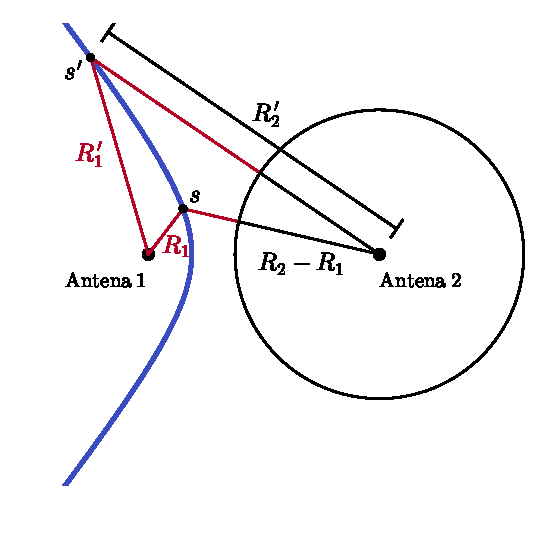
\includegraphics[width=\textwidth]{figuras/example_6_3a.pdf}
  \end{minipage}\hfill
  \begin{minipage}[c]{0.4\textwidth}
    \caption{
       Lugar geométrico de la posición de la fuente para una diferencia de distancia fija a las antenas. Si los tiempos de llegada de la señal emitida a las antenas 1 y 2 son \(t_1\) y \(t_2\) respectivamente, la diferencia de distancia de la fuente a las antenas es \(R_2-R_1=c(t_2-t_1)\), donde \(c\) es la velocidad de propagación de la señal emitida y \(R_1\) y \(R_2\) es la distancia de la fuente a las antenas 1 y 2. El lugar geométrico de los puntos del plano que distan una diferencia de distancia constante a dos puntos fijos (focos) es una hipérbola. Esto implica que la fuente se encuentra en algún punto de la hipérbola.}\label{fig:example_6_3a}
  \end{minipage}
\end{figure}

Se examina a continuación el problema de localización de una fuente usando la teoría de la estimación. Se asume que hay \(N\) antenas en posiciones conocidas y que las medidas de los tiempos de llegada de la señal emitida a cada antena son \(t_i\), con \(i=1,\,\dots,\,N-1\), y el problema consiste en estimar la posición \((x_s,\,y_s)\) de la fuente. Se asume que los tiempos de llegada están contaminados con ruido de media nula y matriz de covarianza conocida, pero de PDF desconocida. Para una señal emitida por la fuente en el instante \(t=T_0\), las medidas se modelan como
\begin{equation}\label{eq:blue_source_localization_toa}
 t_i=T_0+R_i/c+\epsilon_i, \qquad i=0,\,\dots,\,N-1,
\end{equation}
donde los \(\epsilon_i\) son los ruidos de medición y \(c\) es la velocidad de propagación. Se asume que las medidas de ruido son de media nula y varianza \(\sigma^2\) y no correlacionadas entre si. Para continuar, hay que relacionar la distancia \(R_i\) de cada antena a la fuente con la posición desconocida \(\thetabf=[x_s\,y_s]^T\) de la fuente. Siendo \((x_i,\,y_i)\) la posición conocida de la antena \(i\)-ésima, la distancia a la fuente es
\begin{equation}\label{eq:blue_source_localization_range}
 R_i=\sqrt{\left(x_s-x_i\right)^2+\left(y_s-y_i\right)^2}.
\end{equation}
Sustituyendo la ecuación \ref{eq:blue_source_localization_range} en la ecuación \ref{eq:blue_source_localization_toa} se observa que el modelo es no lineal con los parámetros desconocidos \(x_s\) y \(y_s\). Para linealizar el modelo y poder aplicar el teorema de Markov-Gauss, se asume que se conoce la posición nominal \((x_n,\,y_n)\) de la fuente. Esta posición nominal, que es cercana a la posición verdadera, se podría haber obtener de medidas anteriores, situación que es típica en el caso del seguimiento de una fuente. 
\begin{figure}[!htb]
  \begin{minipage}[c]{0.45\textwidth}
    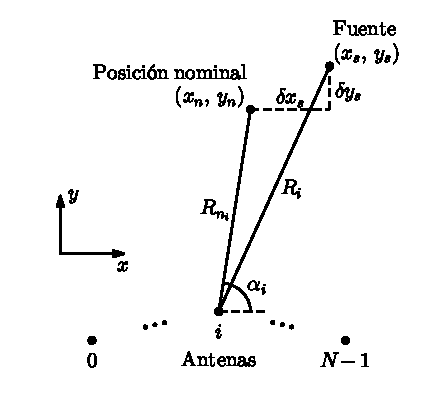
\includegraphics[width=\textwidth]{figuras/example_6_3b.pdf}
  \end{minipage}\hfill
  \begin{minipage}[c]{0.45\textwidth}
    \caption{
       Geometría del problema de localización de fuentes.}\label{fig:example_6_3b}
  \end{minipage}
\end{figure}
Conociendo la posición nominal, se necesita estimar \(\thetabf=[(x_s-x_n)\,(y_s-y_n)]^T=[\delta x_s\,\delta y_s]^T\), indicado en la figura \ref{fig:example_6_3b}. Considérese a \(R_i\) como una función de la posición de la fuente,
\[
 R_i(x,\,y)=\sqrt{\left(x-x_i\right)^2+\left(y-y_i\right)^2}.
\]
Realizando un desarrollo de Taylor de primer orden\footnote{El desarrollo de Taylor de primer orden de una función \(f(x,\,y)\) de dos variables en torno a \((a,\,b)\) es \(f(x,\,y)\approx f(a,\,b)+(x-a)f_x(a,\,b)+(y-b)f_y(a,\,b)\).} en torno a la posición nominal, se tiene que
\[
 R_i(x,\,y)\approx R_i(x_n,\,y_n)+(x-x_n)\frac{\partial R_i(x_n,\,y_n)}{\partial x}+(y-y_n)\frac{\partial R_i(x_n,\,y_n)}{\partial y},
\]
y como
\[
 \frac{\partial R_i(x,\,y)}{\partial x}=\frac{2(x-x_i)}{2\sqrt{\left(x-x_i\right)^2+\left(y-y_i\right)^2}}=\frac{x-x_i}{R_i(x,\,y)}
\]
y análogamente con la derivada respecto a \(y\) se tiene que
\[
 R_i(x,\,y)\approx R_i(x_n,\,y_n)+(x-x_n)\frac{x_n-x_i}{R_i(x_n,\,y_n)}+(y-y_n)\frac{y_n-y_i}{R_i(x_n,\,y_n)}.
\]
Por lo tanto, evaluando en la posición de la fuente, se obtiene que
\[
 R_i(x_s,\,y_s)\approx R_i(x_n,\,y_n)+(x_s-x_n)\frac{x_n-x_i}{R_i(x_n,\,y_n)}+(y_s-y_n)\frac{y_n-y_i}{R_i(x_n,\,y_n)}.
\]
Sean \(R_{n_i}\) las distancias de las antenas a la posición nominal (ver figura \ref{fig:example_6_3b}), la ecuación se puede escribir como
\[
 R_i\approx R_{n_i}+\frac{x_n-x_i}{R_{n_i}}\delta x_s+\frac{y_n-y_i}{R_{n_i}}\delta y_s,
\]
y sustituyendo este resultado en la ecuación \ref{eq:blue_source_localization_toa} se llega a que
\[
 t_i=T_0+\frac{R_{n_i}}{c}+\frac{x_n-x_i}{R_{n_i}c}\delta x_s+\frac{y_n-y_i}{R_{n_i}c}\delta y_s+\epsilon_i,
\]
que ahora es lineal con los parámetros desconocidos \(\delta x_s\) y \(\delta y_s\).
Teniendo en cuenta que
\[
 \frac{x_n-x_i}{R_{n_i}}=\cos\alpha_i\qquad\textrm\qquad \frac{y_n-y_i}{R_{n_i}}=\sin\alpha_i,
\]
donde \(\alpha_i\) se definió en la figura \ref{fig:example_6_3b} el modelo se simplifica como
\[
 t_i=T_0+\frac{R_{n_i}}{c}+\frac{\cos\alpha_i}{c}\delta x_s+\frac{\sin\alpha_i}{c}\delta y_s+\epsilon_i.
\]
El término \(R_{n_i}/c\) es conocido y puede incorporarse a la medida definiendo
\[
 \tau_i=t_i-\frac{R_{n_i}}{c},
\]
por lo que el modelo lineal resulta en
\[
 \tau_i=T_0+\frac{\cos\alpha_i}{c}\delta x_s+\frac{\sin\alpha_i}{c}\delta y_s+\epsilon_i,
\]
donde los parámetros desconocidos son \(T_0\), \(\delta x_s\) y \(\delta y_s\). Si bien el problema ya puede resolverse mediante el teorema de Gauss-Markov, conviene considerar la diferencia de los tiempos de llegada o medidas TDOA para eliminar \(T_0\),
\[
\begin{array}{rcl}
  \xi_1&=&\tau_1-\tau_0\\
  \xi_2&=&\tau_2-\tau_1\\
  &\vdots &\\
  \xi_{N-1}&=&\tau_{N-1}-\tau_{N-2},
 \end{array}
\]
y el modelo lineal final queda
\[
 \xi_i=\frac{1}{c}(\cos\alpha_i-\cos\alpha_{i-1})\delta x_s+\frac{1}{c}(\sin\alpha_i\sin\alpha_{i-1})\delta y_s+\epsilon_i-\epsilon_{i-1},\qquad i=1,\,\dots,\,N-1.
\]
El modelo es de la forma del teorema de Gauss-Markov con
\[
 \thetabf=
 \begin{bmatrix}
  \delta x_s\\
  \delta y_s
 \end{bmatrix}
 \qquad
 \Hbf=\frac{1}{c}
 \begin{bmatrix}
  \cos\alpha_1-\cos\alpha_0 & \sin\alpha_1-\sin\alpha_0\\
  \cos\alpha_2-\cos\alpha_1 & \sin\alpha_2-\sin\alpha_1\\
  \vdots & \vdots\\
  \cos\alpha_{N-1}-\cos\alpha_{N-2} & \sin\alpha_{N-1}-\sin\alpha_{N-2}
 \end{bmatrix}
 \qquad
 \w=
 \begin{bmatrix}
  \epsilon_1-\epsilon_{0}\\
  \epsilon_2-\epsilon_{1}\\
  \vdots\\
  \epsilon_{N-1}-\epsilon_{N-2}
 \end{bmatrix}.
\]
El vector de ruido es de media nula, pero ahora es correlacionado. Para encontrar la matriz de covarianza, se observa que
\[
 \w=
 \underbrace{
 \begin{bmatrix}
  -1 & 1 & 0 & 0 & \dots & 0\\
  0 & -1 & 1 & 0 & \dots & 0\\
  \vdots & \vdots & & \vdots & & \vdots \\
  0 &  0 & \dots & 0 &  -1 & 1
 \end{bmatrix}}_{\displaystyle \A}
 \underbrace{
 \begin{bmatrix}
  \epsilon_0\\
  \epsilon_1\\
  \vdots\\
  \epsilon_{N-1}
 \end{bmatrix}}_{\displaystyle \bm{\epsilon}},
\]
donde la matriz \(\A\) tiene dimensiones \((N-1)\times N\). Por lo tanto, la matriz de covarianza de \(\w\) es
\[
 \C=E(\w\w^T)=E(\A\bm{\epsilon}\bm{\epsilon}^T\A^T)=\A E(\bm{\epsilon}\bm{\epsilon}^T)\A^T=\A(\sigma^2\I)\A^T=\sigma^2\A\A^T.
\]
De la ecuación \ref{eq:blue_estimator_vector} se obtiene que el BLUE de la posición de la fuente es
\begin{align*}
 \hat{\thetabf}&=(\Hbf^T\C^{-1}\Hbf)^{-1}\Hbf^T\C^{-1}\bm{\xi}\\
  &=[\Hbf^T(\A\A^T)^{-1}\Hbf)]^{-1}\Hbf^T(\A\A^T)^{-1}\bm{\xi}
\end{align*}
y de la ecuación \ref{eq:blue_estimator_covariance_vector}, la matriz de covarianza es
\begin{equation}\label{eq:blue_source_localization_covariance}
 \C_{\hat{\thetabf}}=\sigma^2[\Hbf^T(\A\A^T)^{-1}\Hbf)]^{-1}.
\end{equation}


\begin{figure}[!htb]
  \begin{minipage}[c]{0.45\textwidth}
    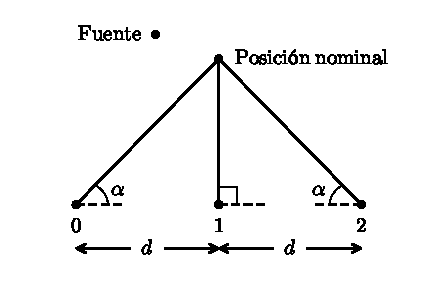
\includegraphics[width=\textwidth]{figuras/example_6_3c.pdf}
  \end{minipage}\hfill
  \begin{minipage}[c]{0.45\textwidth}
    \caption{
       Ejemplo de geometría del problema de localización de fuentes para el conjunto mínimo de antenas.}\label{fig:example_6_3c}
  \end{minipage}
\end{figure}
Como ejemplo, considérese el conjunto de tres antenas mostrado en la figura \ref{fig:example_6_3c}. Para este conjunto mínimo de antenas y la posición nominal indicada, los parámetros del modelo son
\begin{align*}
 \Hbf&=\frac{1}{c}
 \begin{bmatrix}
  \cos\alpha_1-\cos\alpha_0 & \sin\alpha_1-\sin\alpha_0\\
  \cos\alpha_2-\cos\alpha_1 & \sin\alpha_2-\sin\alpha_1
 \end{bmatrix}\\
 &\overset{(a)}{=}\frac{1}{c}
 \begin{bmatrix}
  \cos\pi/2-\cos\alpha & \sin\pi/2-\sin\alpha\\
  \cos(\pi-\alpha)-\cos\pi/2 & \sin(\pi-\alpha)-\sin\pi/2
 \end{bmatrix}\\
 &=\frac{1}{c}
 \begin{bmatrix}
  -\cos\alpha & 1-\sin\alpha\\
  -\cos\alpha & \sin\alpha-1
 \end{bmatrix},
\end{align*}
donde en \((a)\) se consideró que en este caso, \(\alpha_0=\alpha\), \(\alpha_1=\pi/2\) y \(\alpha_2=\pi-\alpha\), y
\[
 \A=
 \begin{bmatrix}
  -1 & 1 & 0\\
  0 & -1 & 1
 \end{bmatrix}.
\]
Se calculará la matriz de covarianza, dada por la ecuación \ref{eq:blue_source_localization_covariance}. Para hacerlo, se ve que
\[
 \A\A^T=
 \begin{bmatrix}
  -1 & 1 & 0\\
  0 & -1 & 1
 \end{bmatrix}
 \begin{bmatrix}
  -1 & 0\\
  1 & -1\\
  0 & 1
 \end{bmatrix}=
 \begin{bmatrix}
  2 & -1\\
  -1 & 2
 \end{bmatrix}
 \qquad\textrm{y}\qquad
 (\A\A^T)^{-1}=\frac{1}{3}
 \begin{bmatrix}
  2 & 1\\
  1 & 2
 \end{bmatrix}.
\]
Luego
\begin{align*}
 (\A\A^T)^{-1}\Hbf&=\frac{1}{3c}
 \begin{bmatrix}
  2 & 1\\
  1 & 2
 \end{bmatrix}
 \begin{bmatrix}
  -\cos\alpha & 1-\sin\alpha\\
  -\cos\alpha & \sin\alpha-1
 \end{bmatrix}\\
 &=\frac{1}{3c}
 \begin{bmatrix}
  -2\cos\alpha-\cos\alpha & 2(1-\sin\alpha)-(1-\sin\alpha)\\
  \cos\alpha-2\cos\alpha & (1-\sin\alpha)-2(1-\sin\alpha)
 \end{bmatrix}\\
 &=\frac{1}{3c}
 \begin{bmatrix}
  -3\cos\alpha & 1-\sin\alpha\\
  -3\cos\alpha & -(1-\sin\alpha)
 \end{bmatrix}
\end{align*}
y
\begin{align*}
  \Hbf^T(\A\A^T)^{-1}\Hbf&=\frac{1}{3c^2}
 \begin{bmatrix}
  -\cos\alpha & -\cos\alpha\\
  1-\sin\alpha & -(1-\sin\alpha)
 \end{bmatrix}
 \begin{bmatrix}
  -3\cos\alpha & 1-\sin\alpha\\
  -3\cos\alpha & -(1-\sin\alpha)
 \end{bmatrix}\\
 &=\frac{1}{3c^2}
 \begin{bmatrix}
  3\cos^2\alpha+3\cos^2\alpha & -(1-\sin\alpha)\cos\alpha+(1-\sin\alpha)\cos\alpha\\
  -3(1-\sin\alpha)\cos\alpha+3(1-\sin\alpha)\cos\alpha & (1-\sin\alpha)^2+(1-\sin\alpha)^2
 \end{bmatrix}\\
 &=\frac{1}{3c^2}
 \begin{bmatrix}
  6\cos^2\alpha & 0\\
  0 & 2(1-\sin\alpha)^2
 \end{bmatrix}\\
 &=\frac{1}{c^2}
 \begin{bmatrix}
  2\cos^2\alpha & 0\\
  0 & \dfrac{2}{3}(1-\sin\alpha)^2
 \end{bmatrix}.
\end{align*}
Como se trata de una matriz diagonal, la matriz inversa es diagonal y sus elementos son los inversos de los elementos de la diagonal, resultando en
\[
 \C_{\hat{\thetabf}}=\sigma^2[\Hbf^T(\A\A^T)^{-1}\Hbf]^{-1}=\sigma^2c^2
 \begin{bmatrix}
  \dfrac{1}{2\cos^2\alpha} & 0\\
  0 & \dfrac{3}{2(1-\sin\alpha)^2}
 \end{bmatrix}.
\]
El resultado muestra que cuando el ángulo \(\alpha\) es mas pequeño se obtiene una localización mas precisa. Esto se logra haciendo que la distancia entre las antenas sea la mayor posible. Además, la localización mejora cuanto menor es la distancia de la fuente a las antenas, ya que esto también reduce el ángulo \(\alpha\).

\section{Problemas}

\subsection{Problema 1}

Si \(x[n]=Ar^n+w[n]\) para \(n=0,\,\dots,\,N-1\), donde \(A\) es un parámetro desconocido, \(r\) es una constante conocida y \(w[n]\) es ruido de media nula y varianza \(\sigma^2\), encontrar el BLUE de \(A\) y la varianza mínima. ¿La varianza mínima tiende a cero cuando \(N\to\infty\)?

\paragraph{Solución} Los datos tienen la forma del modelo de la ecuación \ref{eq:blue_signal_amplitude_model} con \(s[n]=r^n\) y el estimador BLUE y la varianza mínima están dados por las ecuaciones \ref{eq:blue_estimator_scalar} y \ref{eq:blue_estimator_variance_scalar} con \(\C=\sigma^2\I\). Con estos valores, el BLUE es
\[
 \hat{\theta}=\frac{\s^T\C^{-1}\x}{\s^T\C^{-1}\s}=\frac{\displaystyle\frac{1}{\sigma^2}\sum_{n=0}^{N-1}r^nx[n]}{\displaystyle\dfrac{1}{\sigma^2}\sum_{n=0}^{N-1}r^{2n}}
 =\frac{\displaystyle\sum_{n=0}^{N-1}r^nx[n]}{\displaystyle\sum_{n=0}^{N-1}r^{2n}}
\]
y la varianza mínima es
\[
 \var(\hat{\theta})=\frac{1}{\s^T\C^{-1}\s}=\frac{\sigma^2}{\displaystyle\sum_{n=0}^{N-1}r^{2n}}
 \def\arraystretch{2.2}
 =\left\{\begin{array}{ll}
  \dfrac{\sigma^2}{N}, & |r|=1\\
  \dfrac{1-r}{1-r^{2N}}\sigma^2, & |r|\neq1
 \end{array} \right.
\]
Cuando \(N\to\infty\), se cumple que
\[
 \var(\hat{\theta})
 \to\left\{\begin{array}{ll}
  0, & |r|\geq1\\
  (1-r)\sigma^2, & |r|<1
 \end{array} \right.,
\]
es decir, la varianza no tiende a cero si \(|r|<1\).

\subsection{Problema 2}

Se observa
\[
 x[n]=A+w[n],\qquad n=0,\,\dots,\,N-1
\]
donde \(w[n]\) es ruido de media nula, no correlacionado y con varianza \(\var(w[n])=\sigma^2_n\). En el caso en que \(\sigma^2_n=n+1\), examinar que ocurre con la varianza del BLUE cuando \(N\to\infty\). Repetir para el caso en que \(\sigma^2_n=(n+1)^2\) y explicar los resultados.

\paragraph{Solución} La varianza del BLUE está dada por la ecuación \ref{eq:blue_estimator_variance_scalar} con \(\s=\bm{1}\) y matriz de covarianza
\[
 \C=
 \begin{bmatrix}
  \sigma^2_0 & 0 & \dots & 0\\
  0 & \sigma^2_1 & \dots & 0\\
  \vdots & \vdots & \ddots & \vdots\\
  0 & 0 & \dots & \sigma^2_{N-1}
 \end{bmatrix}
 \qquad\Rightarrow\qquad
 \C^{-1}=
 \begin{bmatrix}
  \dfrac{1}{\sigma^2_0} & 0 & \dots & 0\\
  0 & \dfrac{1}{\sigma^2_1} & \dots & 0\\
  \vdots & \vdots & \ddots & \vdots\\
  0 & 0 & \dots & \dfrac{1}{\sigma^2_{N-1}}
 \end{bmatrix}.
\]
Por lo tanto,
\[
 \var(\hat{A})=\frac{1}{\displaystyle\sum_{n=0}^{N-1}\dfrac{1}{\sigma^2_n}}.
\]
En el caso en que \(\sigma^2_n=n+1\),
\[
 \var(\hat{A})=\frac{1}{\displaystyle\sum_{n=0}^{N-1}\dfrac{1}{n+1}}\xrightarrow[N \to \infty]{}0,
\]
ya que el denominador es la serie armónica, la cual diverge.
En el caso en que \(\sigma^2_n=(n+1)^2\), se tiene que
\[
 \var(\hat{A})=\frac{1}{\displaystyle\sum_{n=0}^{N-1}\dfrac{1}{(n+1)^2}}\xrightarrow[N \to \infty]{}\frac{6}{\pi^2},
\]
donde se usó que\footnote{Ver \url{https://en.wikipedia.org/wiki/Basel_problem}}
\[
 \sum_{n=0}^{N-1}\dfrac{1}{(n+1)^2}\xrightarrow[N \to \infty]{}\frac{\pi^2}{6}.
\]
En este caso, la varianza de las muestras de ruido es tan grande que la varianza del estimador no tiende a cero.

\subsection{Problema 3}

Se considera el problema de la estimación de DC (ver el problema anterior) pero ahora las muestras de ruido están correlacionadas con matriz de covarianza 
\[
 \C=\sigma^2
 \begin{bmatrix}
  \begin{matrix}
   1 & \rho \\
   \rho & 1
  \end{matrix} & \bm{0} & \dots & \bm{0}\\
  \bm{0} &
  \begin{matrix}
   1 & \rho \\
   \rho & 1
  \end{matrix} & \dots & \bm{0}\\
  \vdots & \vdots & \ddots & \vdots \\
  \bm{0} & \bm{0} & \dots &
  \begin{matrix}
   1 & \rho \\
   \rho & 1
  \end{matrix}
 \end{bmatrix},
\]
donde \(|\rho|<1\) y la dimensión \(N\) de la matriz es un número par. \(\C\) es una matriz diagonal a bloques y por lo tanto, fácil de invertir. Encontrar el BLUE y su varianza e interpretar los resultados.

\paragraph{Solución} La matriz de covarianza indica que las muestras están correlacionadas de a pares, es decir, la muestra \(w[n]\) esta correlacionada con la muestra \(w[n+1]\), con \(n\) par, pero no con el resto de las muestras. El BLUE y su varianza están dados por las ecuaciones \ref{eq:blue_estimator_scalar} y \ref{eq:blue_estimator_variance_scalar} con \(\s=\bm{1}\). Para encontrarlos, es necesario invertir la matriz \(\C\). La matriz \(\C\) es diagonal a bloques, y cada bloque es
\[
 \C_{ii}=\sigma^2
 \begin{bmatrix}
  1 & \rho\\
  \rho & 1
 \end{bmatrix}
 \qquad\Rightarrow\qquad
 \C_{ii}^{-1}=\frac{1}{\sigma^2(1-\rho^2)}
 \begin{bmatrix}
  1 & -\rho\\
  -\rho & 1
 \end{bmatrix}.
\]
Por lo tanto, la inversa de la matriz de covarianza es (ver el apéndice \ref{ap:block_matrix_properties})
\[
 \C^{-1}=\frac{1}{\sigma^2(1-\rho^2)}
 \begin{bmatrix}
  \begin{matrix}
   1 & -\rho \\
   -\rho & 1
  \end{matrix} & \bm{0} & \dots & \bm{0}\\
  \bm{0} &
  \begin{matrix}
   1 & -\rho \\
   -\rho & 1
  \end{matrix} & \dots & \bm{0}\\
  \vdots & \vdots & \ddots & \vdots \\
  \bm{0} & \bm{0} & \dots &
  \begin{matrix}
   1 & -\rho \\
   -\rho & 1
  \end{matrix}
 \end{bmatrix},
\]
Luego,
\[
 \C^{-1}\x=\frac{1}{\sigma^2(1-\rho^2)}
 \begin{bmatrix}
  x[0]-\rho x[1]\\
  -\rho x[0]+x[1]\\
  x[2]-\rho x[3]\\
  -\rho x[2]+x[3]\\
  \vdots\\
  x[N-2]-\rho x[N-1]\\
  -\rho x[N-2]+x[N-1]
 \end{bmatrix}
\]
y
\begin{align}\label{eq:problem_6_3_estimator_numerator}
 \bm{1}^T\C^{-1}\x&=\frac{1}{\sigma^2(1-\rho^2)}\left(\sum_{n=0}^{N-1}x[n]-\sum_{n=0}^{N-1}\rho x[n]\right)\nonumber\\
 &=\frac{1}{\sigma^2(1-\rho^2)}(1-\rho)\sum_{n=0}^{N-1}x[n]\nonumber\\
 &\overset{(a)}{=}\frac{1}{\sigma^2(1+\rho)}\sum_{n=0}^{N-1}x[n],
\end{align}
donde en \((a)\) se observó que \((1-\rho^2)=(1+\rho)(1-\rho)\). Además,
\[
 \C^{-1}\bm{1}=\frac{1}{\sigma^2(1-\rho^2)}(1-\rho)\bm{1}=\frac{1}{\sigma^2(1+\rho)}\bm{1}
\]
y
\begin{equation}\label{eq:problem_6_3_estimator_denominator}
 \bm{1}^T\C^{-1}\bm{1}=\frac{N}{\sigma^2(1+\rho)}.
\end{equation}
De las ecuaciones \ref{eq:problem_6_3_estimator_numerator} y \ref{eq:problem_6_3_estimator_denominator} se obtiene que el BLUE es
\[
 \hat{A}=\frac{\bm{1}^T\C^{-1}\x}{\bm{1}^T\C^{-1}\bm{1}}=\frac{1}{N}\sum_{n=0}^{N-1}x[n]=\bar{x},
\]
con varianza
\[
 \var(\hat{A})=\frac{1}{\bm{1}^T\C^{-1}\bm{1}}=\frac{\sigma^2(1+\rho)}{N}.
\]
Se observa que en el caso en que \(\rho=0\), que implica que las muestras no están correlacionadas, \(\var(\hat{A})=\sigma^2/N\), que es el caso usual. Si \(\rho\to1\), los pares de muestras están totalmente correlacionados y \(\var(\hat{A})\to2\sigma^2/N\) ya que la correlación total de a pares implica que \(x[n]=x[n+1]\), lo que es equivalente a observar la mitad de las muestras. Finalmente, si \(\rho\to-1\), \(\var(\hat{A})\to0\), ya que esto implica que \(w[n]=-w[n+1]\) y de esta forma
\[
 \frac{x[n]+x[n+1]}{2}=\frac{(A+w[n])+(A-w[n])}{2}=A,
\]
es decir, el promediado de dos muestras sucesivas produce el valor exacto de \(A\) (ver el problema de la sección \ref{sec:problem_3_9}).

\subsection{Problema 4}

Se observan las muestras \(\{x[0],\,x[1],\,\dots,\,x[N-1]\}\) IID con las siguientes PDFs:
\begin{enumerate}[a.]
 \item Laplaciana
 \[
  p(x[n];\,\mu)=\frac{1}{2}\exp[-|x[n]-\mu|]
 \]
 \item Gaussiana
 \[
  p(x[n];\,\mu)=\frac{1}{\sqrt{2\pi}}\exp\left[-\frac{1}{2}(x[n]-\mu)^2\right]
 \]
\end{enumerate}
Encontrar el BLUE de la media \(\mu\) en ambos casos. ¿Qué se puede decir sobre el estimador MVU de \(\mu\)?

\paragraph{Solución} Los datos se modelan como 
\[
 \x=\mu\bm{1}+\w, \qquad \textrm{con}\qquad E(\w)=\bm{0}\qquad\textrm{y}\qquad \C=E(\w\w^T)=\var(w[n])\I. 
\]
El BLUE está dado por la ecuación \ref{eq:blue_estimator_scalar} con \(\s=\bm{1}\), y es
\[
 \hat{\mu}=\frac{\bm{1}^T\C^{-1}\x}{\bm{1}^T\C^{-1}\bm{1}}=\frac{\bm{1}^T\x}{\bm{1}^T\bm{1}}
 =\frac{1}{N}\sum_{n=0}^{N-1}x[n]=\bar{x}
\]
En el caso gaussiano, la media muestral es el estimador MVU, y por lo tanto, el BLUE produce el estimador MVU. Esto se debe a que el estimador MVU es lineal con los datos. En el caso de datos con distribución de Laplace, para afirmar que la media muestral es el estimador MVU, habría que calcular la CRLB y ver si la varianza de la media muestral alcanza la cota, o encontrar un estimador mediante el método de los estadísticos suficientes y ver que el  estimador es la media muestral. Si se intentara alguno de estos dos métodos para encontrar el estimador MVU, se parte observando que la PDF de los datos es
\[
 p(\x;\,\mu)=\frac{1}{2^N}\exp\left(-\sum_{n=0}^{N-1}|x[n]-\mu|\right).
\]
Para encontrar un estadístico suficiente, la PDF debe factorizarse como la ecuación \ref{eq:general_mvu_neyman_fisher_factorization} del teorema de Neyman-Fisher. Esto no parece ser posible, ya que el valor absoluto impide separar los datos del parámetro en una función \(g(T(\x),\,\mu)\). Para calcular la CRLB, tomando el logaritmo, se tiene que
\[
 \ln p(\x;\,\mu)=-N\ln2-\sum_{n=0}^{N-1}|x[n]-\mu|
\]
y derivando respecto al parámetro, llega a que
\begin{align*}
 \frac{\partial \ln p(\x;\,\mu)}{\partial \mu}=-\sum_{n=0}^{N-1}\frac{\partial|x[n]-\mu|}{\partial \mu}=\sum_{n=0}^{N-1}\operatorname{sig}(x[n]-\mu),
\end{align*}
función que parece no poder ser factorizada como la ecuación \ref{eq:crlb_efficiency_condition}. Se concluye que no es posible afirmar si la media muestral es el estimador MVU a partir de estadísticos suficientes o mediante la CRLB.

\subsection{Problema 5}

Se oservan las muestras \(\{x[0],\,\dots,\,x[N-1]\}\) IID con PDF log-normal
\[
 p(x[n],\,\theta)
 \def\arraystretch{2.2}
 =\left\{\begin{array}{ll}
  \dfrac{1}{\sqrt{2\pi}x[n]}\exp\left[-\dfrac{1}{2}(\ln x[n]-\theta)^2\right], & x[n]>0\\
  0, & x[n]<0
 \end{array} \right.
\]
Probar que la media es \(\exp(\theta+1/2)\) y por lo tanto, no puede satisfacerse la restricción de insesgado del estimador lineal. Usando el enfoque de la transformación de variables aleatorias con \(y[n]=\ln x[n]\), encontrar el BLUE para \(\theta\).

\paragraph{Solución} Partiendo de la definición de la media, se ve que
\begin{align*}
 E(x[n])&=\int_{-\infty}^{\infty}xp(x;\,\theta)\,dx\\
   &=\int_{0}^{\infty}x\frac{1}{\sqrt{2\pi}x}e^{-\frac{1}{2}(\ln x-\theta)^2}\,dx\\
   &=\int_{0}^{\infty}\frac{1}{\sqrt{2\pi}}e^{-\frac{1}{2}(\ln x-\theta)^2}\,dx\\
   &\overset{(a)}{=}\int_{-\infty}^{\infty}\frac{1}{\sqrt{2\pi}}e^{u+\theta}e^{-\frac{1}{2}u^2}\,du\\
   &=e^\theta\int_{-\infty}^{\infty}\frac{1}{\sqrt{2\pi}}e^{-\frac{1}{2}(u^2-2u)}\,du,\\
   &\overset{(b)}{=}e^{\theta+\frac{1}{2}}\int_{-\infty}^{\infty}\frac{1}{\sqrt{2\pi}}e^{-\frac{1}{2}(u-1)^2}\,du\\
   &\overset{(c)}{=}e^{\theta+\frac{1}{2}},
\end{align*}
donde en \((a)\) se realizó el cambio de variable \(u=\ln x-\theta\), \(du=dx/x\) y como \(x=\exp(u+\theta)\), \(dx=\exp(u+\theta)du\). Notar además que el límite inferior de integración es \(u=-\infty\), ya que \(u=\ln x-\theta\to-\infty\) cuando \(x\to0\). En \((b)\) se empleó la técnica de ``completar el cuadrado'' observando que
\[
 e^{-\frac{1}{2}(u-1)^2}=e^{-\frac{1}{2}(u^2-2u-1)}=e^{-\frac{1}{2}(u^2-2u)}e^{-\frac{1}{2}}
\]
y por lo tanto,
\[
 e^{-\frac{1}{2}(u^2-2u)}=e^{-\frac{1}{2}(u-1)^2}e^{\frac{1}{2}},
\]
y en \((c)\) que el resultado de la integral es 1 por tratarse de la integral en todo el dominio de una PDF \(\mathcal{N}(1,\,1)\). Se concluye que \(E(x[n])=\exp(\theta+1/2)\), que es lo que se quería demostrar.

La restricción para que el BLUE sea insesgado es
\[
 E(\hat{\theta})=\sum_{n=0}^{N-1}a_nE(x[n])=\theta,
\]
y en este caso la condición queda
\[
 \sum_{n=0}^{N-1}a_ne^{\theta+\frac{1}{2}}+\theta\qquad\Rightarrow\qquad\sum_{n=0}^{N-1}a_n=\frac{\theta}{e^{\theta+\frac{1}{2}}},
\]
igualdad que no puede cumplirse para todo valor de \(\theta\).

Se considera ahora la transformación de la variable aleatoria \(y=g(x)=\ln x\). La PDF de la variable transformada está dada por la ecuación \ref{eq:general_mvu_rv_transformation} y como en este caso, a cada valor de \(y\) corresponde un único valor de \(x\) se tiene que
\[
 p_y(y)=\frac{p_x(x)}{|g'(x)|}=\frac{p_x(e^y)}{\dfrac{1}{e^y}},
\]
donde en la última igualdad se consideró que \(g'(x)=1/x\) y que \(x=e^y\). Por lo tanto, la PDF de \(y[n]=\ln x[n]\) es
\begin{align*}
 p(y[n];\,\theta)&=\frac{\dfrac{1}{\sqrt{2\pi}e^y[n]}\exp\left[-\dfrac{1}{2}(y[n]-\theta)^2\right]}{\dfrac{1}{e^{y[n]}}}\\
  &=\frac{1}{\sqrt{2\pi}}\exp\left[-\dfrac{1}{2}(y[n]-\theta)^2\right],
\end{align*}
es decir, \(y[n]\sim\mathcal{N}(\theta,\,1)\), y por lo tanto, el BLUE para \(\theta\) es la media muestral
\[
 \hat{\theta}=\frac{1}{N}\sum_{n=0}^{N-1}y[n]=\frac{1}{N}\sum_{n=0}^{N-1}\ln x[n].
\]

\subsection{Problema 6}

En este problema se extiende el resultado del BLUE escalar. Asúmase que \(E(x[n])=\theta s[n]+\beta\), donde \(\theta\) es el parámetro desconocido a estimar y \(\beta\) es una constante conocida. El vector \(\x\) de datos tiene matriz de covarianza \(\C\). Se define un estimador lineal (en realidad, afín) para este problema como
\[
 \hat{\theta}=\sum_{n=0}^{N-1}a_nx[n]+b.
\]
Probar que el BLUE está dado por
\[
 \hat{\theta}=\frac{\s^T\C^{-1}(\x-\beta\bm{1})}{\s^T\C^{-1}\s}.
\]
Además, encontrar la varianza mínima.

\paragraph{Solución} La condición de que el estimador sea insesgado es
\[
 E(\hat{\theta})=\sum_{n=0}^{N-1}a_nE(x[n])+b=\theta,
\]
y sustituyendo \(E(x[n])\) se obtiene que
\[
 \sum_{n=0}^{N-1}a_n(\theta s[n]+\beta)+b=\theta\qquad\qquad\textrm{o}\qquad\qquad
 \theta\sum_{n=0}^{N-1}a_ns[n]+\sum_{n=0}^{N-1}a_n\beta+b=\theta.
\]
de lo que se deduce que las condiciones para que el estimador sea insesgado son
\[
 \sum_{n=0}^{N-1}a_ns[n]=1\qquad\qquad\textrm{y}\qquad\qquad \sum_{n=0}^{N-1}a_n\beta=-b.
\]
Sustituyendo \(b\) en el estimador, queda
\[
 \hat{\theta}=\sum_{n=0}^{N-1}a_nx[n]-\sum_{n=0}^{N-1}a_n\beta=\sum_{n=0}^{N-1}a_n(x[n]-\beta)
\]
y finalmente, definiendo \(x'[n]=x[n]-\beta\)
\[
 \hat{\theta}=\sum_{n=0}^{N-1}a_nx'[n]
\]
que es el estimador lineal usual, pero ahora el vector de datos es \(\x'=\x-\beta\bm{1}\), que tiene la misma matriz de covarianza que \(\x\). Por lo tanto, el BLUE es
\[
 \hat{\theta}=\frac{\s^T\C^{-1}\x'}{\s^T\C^{-1}\s}=\frac{\s^T\C^{-1}(\x-\beta\bm{1})}{\s^T\C^{-1}\s}
\]
y la varianza mínima es
\[
 \var(\theta)=\frac{1}{\s^T\C^{-1}\s}.
\]

\subsection{Problema 7}

Se asume que se observa \(x[n]=As[n]+w[n]\) para \(n=0,\,\dots,\,N-1\), donde \(w[n]\) es rido de media nula con matriz de covarianza \(\C\) y \(s[n]\) es una señal conocida. Se desea encontrar el estimador BLUE de la amplitud \(A\). Calcular el estimador BLUE y discutir que ocurre si \(\s=[s[0]\,\dots\,s[N-1]]^T\) es un vector propio de \(\C\). Además, calcular la variannza mínima.

\paragraph{Solución} El estimador BLUE de \(A\) es
\[
 \hat{A}=\frac{\s^T\C^{-1}\x}{\s^T\C^{-1}\s}.
\]
Si \(\s\) es un vector propio de \(\C\) con valor propio \(\lambda\), \(\s\) también es vector propio de \(\C^{-1}\) con valor propio \(1/\lambda\), es decir, se cumple que
\[
 \C^{-1}\s=\frac{1}{\lambda}\s
\]
y por lo tanto, también que
\[
 \s^T\C^{-1}=(\C^{-1}\s)^T=\frac{1}{\lambda}\s^T,
\]
donde se consideró que además \(\C^{-1}\) es una matriz simétrica. Sustituyendo estos resultados, el estimador queda
\[
 \hat{A}=\frac{\s^T\x}{\s^T\s}.
\]
Notar que el resultado es el mismo que en el caso en que \(\C=\sigma^2\I\). La varianza mínima es
\[
 \var(\hat{A})=\frac{\lambda}{\s^T\s}.
\]

\subsection{Problema 8}

Continuando con el problema anterior, siempre es posible representar al vector señal \(\s\) como una combinación lineal de vectores propios de \(\C\). Esto se debe a que \(\C\) tiene \(N\) vectores propios linealmente independientes. Además, puede mostrarse que debido a la naturaleza simétrica de \(\C\), esos vectores propios son ortonormales. Por lo tanto, una representación ortogonal de la señal es
\[
 \s=\sum_{i=0}^{N-1}\alpha_i\vbf_i,
\]
donde \(\{\vbf_0,\,\dots,\,\vbf_{N-1}\}\) son los vectores propios ortonormales de \(\C\). Probar que la varianza mínima del BLUE es
\[
 \var(\hat{A})=\frac{1}{\displaystyle\sum_{i=0}^{N-1}\frac{\alpha_i^2}{\lambda_i}},
\]
donde \(\lambda_i\) es el valor propio de \(\C\) asociado al vector propio \(\vbf_i\).
Luego, mostrar que la energía de la señal \(\mathcal{E}=\s^T\s\) está dada por \(\sum_{i=0}^{N-1}\alpha_i^2\). Finalmente, probar que si la energía se restringe a ser cierto valor \(\mathcal{E}_0\), la menor varianza posible del BLUE se obtiene eligiendo la señal 
\[
 \s=c\vbf_\textrm{min},
\]
donde \(\vbf_\textrm{min}\) es el vector propio de \(\C\) asociado al menor valor propio y \(c\) se elige de forma de satisfacer la restricción de la energía \(\mathcal{E}_0=\s^T\s=c^2\). Asumir que los valores propios de \(\C\) son todos distintos. Explicar porque este resultado tiene sentido.

\paragraph{Solución} Se mostrará primero informalmente, que los vectores propios de una matriz simétrica son ortogonales. Este resultado está dado por el teorema espectral. Supóngase que \(\x\) y \(\y\) son vectores propios de la matriz simétrica \(\A\) con valores propios asociados \(\lambda\) y \(\mu\) distintos. En este caso, se cumple que
\[
 \lambda\x^T\y=(\lambda\x)^T\y=(\A\x)^T\y=\x^T\A^T\y=\x^T\A\y=\x^T\mu\y
\]
y por lo tanto,
\[
 (\lambda-\mu)\x^T\y=0\qquad\Rightarrow\qquad \x^T\y=0,
\]
es decir, \(\x\) e \(\y\) son ortonormales. Faltaría considerar el caso en que los valores propios son iguales, pero no se hará aquí.

La varianza mínima del estimador BLUE es
\[
 \var(\hat{A})=\frac{1}{\s^T\C^{-1}\s}.
\]
Por lo tanto, considerando la representación de \(\s\) como combinación lineal de los vectores propios, se tiene que
\begin{align*}
 \C^{-1}\s&=\C^{-1}\sum_{j=0}^{N-1}\alpha_j\vbf_j\\
   &=\sum_{j=0}^{N-1}\alpha_j\C^{-1}\vbf_j\\
   &=\sum_{j=0}^{N-1}\frac{\alpha_j}{\lambda_j}\vbf_j,
\end{align*}
donde en la última igualdad se consideró que si \(\lambda_j\) es el valor propio de \(\C\) asociado al vector propio \(\vbf_j\), \(1/\lambda_j\) es el valor propio de \(\C^{-1}\) asociado al vector propio \(\vbf_j\). Luego,
\begin{align*}
 \s^T\C^{-1}\s&=\left(\sum_{i=0}^{N-1}\alpha_i\vbf_i\right)^T\sum_{j=0}^{N-1}\frac{\alpha_j}{\lambda_j}\vbf_j\\
   &=\sum_{i=0}^{N-1}\alpha_i\vbf_i^T\sum_{j=0}^{N-1}\frac{\alpha_j}{\lambda_j}\vbf_j\\
   &=\sum_{i=0}^{N-1}\sum_{j=0}^{N-1}\frac{\alpha_i\alpha_j}{\lambda_j}\vbf_i^T\vbf_j\\
   &=\sum_{i=0}^{N-1}\frac{\alpha_i^2}{\lambda_i},
\end{align*}
donde en la última igualdad se consideró que los vectores propios son ortogonales, es decir, cumplen que
\[
 \vbf_i^T\vbf_j=
 \left\{
 \begin{array}{ll}
  1, &  \textrm{si }i=j\\
  0, &  \textrm{si }i\neq j.
 \end{array}\right.
\]
Se concluye que
\[
 \var(\hat{A})=\frac{1}{\displaystyle\sum_{i=0}^{N-1}\frac{\alpha_i^2}{\lambda_i}},
\]
que es lo que se quería demostrar.

La energía de la señal es
\begin{align*}
 \mathcal{E}&=\s^T\s\\
  &=\sum_{i=0}^{N-1}\alpha_i\vbf_i^T\sum_{j=0}^{N-1}\alpha_j\vbf_j\\
  &=\sum_{i=0}^{N-1}\sum_{j=0}^{N-1}\alpha_i\alpha_j\vbf_i^T\vbf_j\\
  &=\sum_{i=0}^{N-1}\alpha_i^2,
\end{align*}
donde nuevamente se consideró que los vectores propios son ortonormales.

Por último, se quiere encontrar la señal de energía \(\mathcal{E}_0\) que minimiza la varianza. El problema consiste en buscar los valores de \(\alpha_i\) que maximicen el denominador \(\sum_{i=0}^{N-1}\alpha_i^2/\lambda_i\) de la varianza sujeto a la restricción \(\sum_{i=0}^{N-1}\alpha_i^2=\mathcal{E}_0\) de la energía de la señal. Considerando multiplicadores de Lagrange, esto implica encontrar los puntos estacionarios de la función
\[
 \mathcal{L}(\bm{\alpha},\,\lambda)=\sum_{i=0}^{N-1}\frac{\alpha_i^2}{\lambda_i}+\lambda\left(\sum_{i=0}^{N-1}\alpha_i^2-\mathcal{E}_0\right).
\]
Derivando respecto a \(\alpha_k\), se tiene que
\[
 \frac{\partial\mathcal{L}(\bm{\alpha},\,\lambda)}{\partial\alpha_k}=\frac{2\alpha_k}{\lambda_k}+2\lambda\alpha_k
\]
e igualando a cero, se obtienen las condiciones
\[
 \alpha_k\left(\frac{1}{\lambda_k}+\lambda\right)=0,\qquad k=0,\dots,\,N-1.
\]
Esto significa que \(\alpha_k=0\) o \(\lambda=-1/\lambda_k\) para todo \(k\). Pero por la hipótesis de que los valores propios de \(\C\) son todos distintos, \(\lambda=-1/\lambda_k\) a lo sumo solo para un valor de \(k\). Adicionalmente, no puede ocurrir que \(\alpha_k=0\) para todo \(k\) ya que no se cumpliría la restricción de la energía de la señal. Por lo tanto, la única posibilidad es que \(\alpha_k=0\) para todo \(k\) excepto para uno solo. Sea este \(k=j\), donde \(j\) es el índice asociado al menor valor propio. De esta forma, \(\alpha_k=0\) para todo \(k\) excepto para \(k=j\) y \(\lambda=1/\lambda_j\) por lo que
\[
 \s=\alpha_j\vbf_j\qquad\qquad\textrm{y}\qquad\qquad\mathcal{E}_0=\alpha_j^2
\]
y la varianza del estimador es
\[
 \var(\hat{A})=\frac{1}{\dfrac{\alpha_j^2}{\lambda_j}}=\frac{\lambda_j}{\alpha^2_j}=\frac{\lambda_j}{\mathcal{E}_0},
\]
es decir
\[
 \var(\hat{A})=\frac{\lambda_\textrm{mín}}{\mathcal{E}_0}\qquad\qquad\textrm{con}\qquad\qquad
 \s=c\vbf_\textrm{mín}=\sqrt{\mathcal{E}_0}\vbf_\textrm{mín}.
\]


\subsection{Problema 9}

En un sistema de comunicación de encendido y apagado (\emph{on-off keyed}, OOK) se transmite una de dos señales
\[
 s_0(t)=0,\qquad 0\leq t\leq T
\]
para representar un 0 binario o
\[
 s_1(t)=A\cos2\pi f_1t,\qquad 0\leq t\leq T 
\]
para representar un 1 binario. Se asume que la amplitud \(A\) es positiva. Para determinar que bit fue transmitido, se muestrea la señal recibida obteniendo
\[
 x[n]=s_i[n]+w[n],\qquad n=0,\,\dots,\,N-1.
\]
Si se transmitió un 0, \(s_i[n]=0\), y si se transmitió un 1, \(s_i[n]=A\cos2\pi f_1 n\) (asumiendo una tasa de muestreo de 1 muestra/s). Las muestras de ruido \(w[n]\) modelan el ruido del canal. Un receptor sencillo podría estimar la amplitud \(A\) de la sinusoide y decidir que se envió un 1 si \(\hat{A}>\gamma\) y un 0 si \(\hat{A}<\gamma\). De esta forma, un problema equivalente es estimar la amplitud \(A\) de la señal recibida
\[
 x[n]=A\cos2\pi f_1n+w[n],\qquad n=0,\,\dots,\,N-1,
\]
donde \(w[n]\) es ruido de media nula con matriz de covarianza \(\C=\sigma^2\I\). Encontrar el BLUE para este problema e interpretar el detector resultante. Encontrar la mejor frecuencia en el rango \(0\leq f_1<1/2\) para usar en el transmisor.

\paragraph{Solución} El modelo de los datos es en este caso
\[
 x[n]=As[n]+w[n],\qquad\textrm{con}\qquad s[n]=\cos2\pi f_1n. 
\]
Con \(\s=[1\,\cos2\pi f_1,\,\dots,\,\cos2\pi f_1(N-1)]^T\), el estimador BLUE es
\[
 \hat{A}=\frac{\s^T\C^{-1}\x}{\s^T\C^{-1}\s}=\frac{\s^T\x}{\s^T\s}
  =\frac{\displaystyle\sum_{n=0}^{N-1}s[n]x[n]}{\displaystyle\sum_{n=0}^{N-1}s^2[n]}
  =\frac{\displaystyle\sum_{n=0}^{N-1}x[n]\cos2\pi f_1n}{\displaystyle\sum_{n=0}^{N-1}\cos^22\pi f_1n}.
\]
Observando que el estimador puede escribirse como
\[
 \hat{A}=\frac{\dfrac{N}{2}}{\displaystyle\sum_{n=0}^{N-1}\cos^22\pi f_1n}\frac{2}{N}\sum_{n=0}^{N-1}x[n]\cos2\pi f_1n
\]
y que
\[
 \frac{\dfrac{N}{2}}{\displaystyle\sum_{n=0}^{N-1}\cos^22\pi f_1n}
 \overset{(a)}{=}
 \frac{\dfrac{N}{2}}{\displaystyle\sum_{n=0}^{N-1}\frac{1+\cos4\pi f_1n}{2}}
 =\frac{N}{N+\displaystyle\sum_{n=0}^{N-1}\cos4\pi f_1n}
 =\frac{1}{1+\displaystyle\frac{1}{N}\sum_{n=0}^{N-1}\cos4\pi f_1n}
 \overset{(b)}{\approx}1,
\]
donde en \((a)\) se empleó la identidad trigonométrica \(\cos(2\theta )=2\cos^{2}\theta-1\) y en \((b)\) se tuvo en cuenta que \(\frac{1}{N}\sum_{n=0}^{N-1}\cos4\pi f_1n\approx0\) si \(f_1\) no es cercano a 0 ni a 1/2, como se mostró en el problema de la sección \ref{sec:problem_3_7}, se obtiene que
\[
 \hat{A}\approx\frac{2}{N}\sum_{n=0}^{N-1}x[n]\cos2\pi f_1n
\]
si \(f_1\) no es cercano a 0 ni a 1/2. Se concluye que el estimador de la amplitud es el coeficiente de Fourier correspondiente al coseno de frecuencia \(f_1\) (ver la ecuación \ref{eq:rdft} del apéndice \ref{ap:rdft}). Además, la varianza es
\[
 \var(\hat{A})=\frac{1}{\s^T\C^{-1}\s}=\frac{\sigma^2}{\s^T\s}
  =\frac{\sigma^2}{\displaystyle\sum_{n=0}^{N-1}\cos^22\pi f_1n}\geq\frac{\sigma^2}{N},
\]
ya que \(\sum_{n=0}^{N-1}\cos^22\pi f_1n\leq N\) y la igualdad se da si \(f_1=0\). Por lo tanto, la varianza se minimiza si se emplea una señal constante. Con esta elección, se maximiza la energía de la señal. En la figura \ref{fig:problem_6_9} se muestra la varianza del estimador en función de la frecuencia de la sinusoide enviada.
\begin{figure}[!htb]
  \begin{minipage}[c]{0.68\textwidth}
    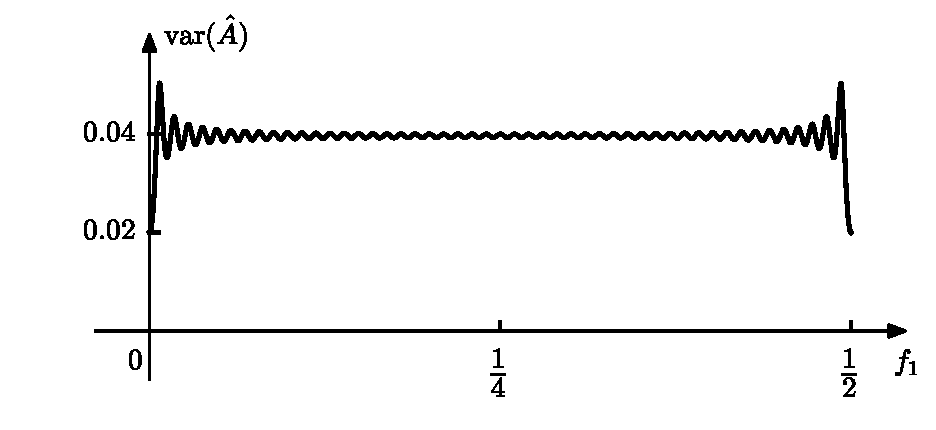
\includegraphics[width=\textwidth]{figuras/problem_6_9.pdf}
  \end{minipage}\hfill
  \begin{minipage}[c]{0.22\textwidth}
    \caption{
       Varianza del estimador \(\hat{A}\) en función de la frecuencia \(f_1\) de la sinusoide enviada para \(N=50\) y \(\sigma^2=1\).
    } \label{fig:problem_6_9}
  \end{minipage}
\end{figure}


\subsection{Problema 10}\label{sec:problem_6_10}

En este problema se continúa el problema anterior examinando la selección de la señal para un sistema OOK en la presencia de ruido coloreado. Sea el ruido \(w[n]\) un proceso aleatorio WSS de media nula con ACF
\[
 r_{ww}[k]=
 \left\{
 \begin{array}{cl}
  1.81 &  k=0\\
  0 &  k=1\\
  0.9 & k=2\\
  0 & k\geq 3
 \end{array}\right.
\]
Encontrar y graficar la PSD para las frecuencias \(0\geq f\geq 1/2\). Como en el problema anterior, encontrar la frecuencia que produce la menor varianza del BLUE para \(N=50\). Explicar los resultados. Sugerencia: se necesita una computadora para hacerlo.

\paragraph{Solución} La PSD \(P_{ww}(f)\) del ruido es la transformada de Fourier de la autocorrelación,
\begin{align*}
 P_{ww}(f)&=\mathcal{F}\{r_{ww}[k]\}\\
  &=\sum_{k=-\infty}^{\infty}r_{ww}[k]e^{-j2\pi fk}\\
  &=r_{ww}[-2]e^{j4\pi f}+r_{ww}[0]+r_{ww}[2]e^{-j4\pi f}\\
  &=r_{ww}[0]+r_{ww}[2]\left(e^{j4\pi f}+e^{-j4\pi f}\right)\\
  &=r_{ww}[0]+2r_{ww}[2]\cos4\pi f,
\end{align*}
resultando en
\[
 P_{ww}(f)=1.81+1.8\cos4\pi f,
\]
y se muestra en la figura \ref{fig:problem_6_10}.
\begin{figure}[!htb]
  \begin{minipage}[c]{0.68\textwidth}
    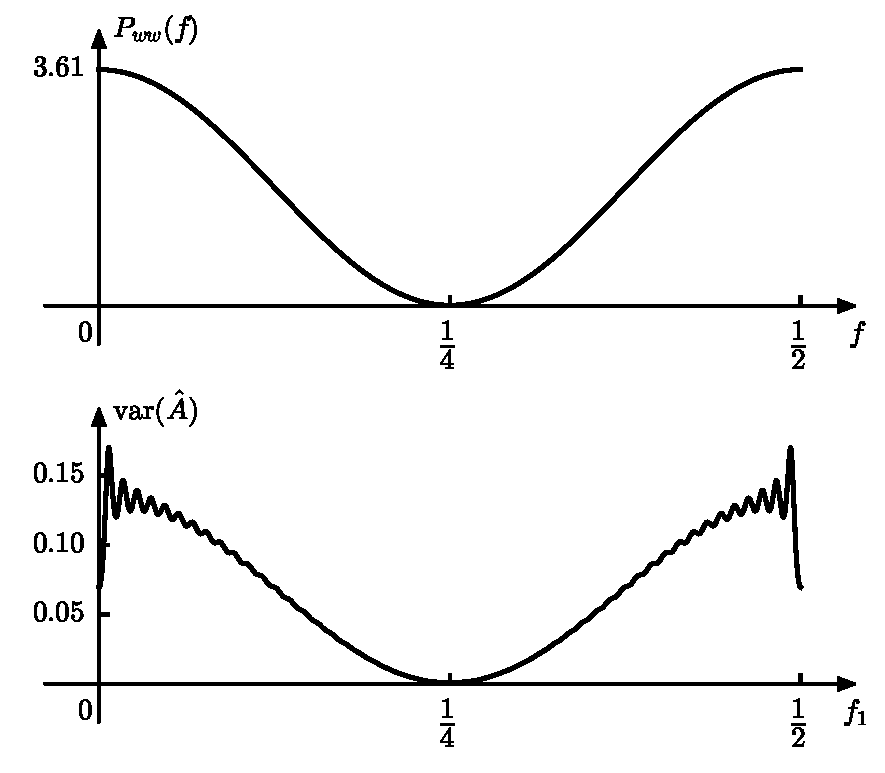
\includegraphics[width=\textwidth]{figuras/problem_6_10.pdf}
  \end{minipage}\hfill
  \begin{minipage}[c]{0.22\textwidth}
    \caption{
       PSD del ruido coloreado y varianza del estimador BLUE. La varianza del estimador es menor en las frecuencias donde el ruido tiene menor potencia.
    } \label{fig:problem_6_10}
  \end{minipage}
\end{figure}
Para ver en que frecuencias el estimador tiene menor varianza, hay que calcular la varianza en función de la frecuencia \(f_1\) de la señal transmitida. La varianza del estimador es
\[
 \var(\hat{A})=\frac{1}{\s^T\C^{-1}\s},
\]
con \(\s=[1\,\cos2\pi f_1,\,\dots,\,\cos2\pi f_1(N-1)]^T\), y la matriz de covarianza de los datos es
\[
 \C=
 \begin{bmatrix}
 r_{ww}[0] & r_{ww}[1] & \dots & r_{ww}[N-1]\\    
 r_{ww}[1] & r_{ww}[0] & \dots & r_{ww}[N-2]\\
  \vdots   &  \vdots & \ddots & \vdots \\
 r_{ww}[N-1] & r_{ww}[N-2] & \dots & r_{ww}[0]
 \end{bmatrix}
 =
 \begin{bmatrix}
 1.81 & 0 & 0.9 & 0 & \dots & 0\\    
 0 & 1.81 & 0 & 0.9 & \dots & 0\\
 0.9 & 0 & 1.81 & 0 & \dots & 0\\
 \vdots & \ddots & \ddots & \ddots & \ddots & \vdots \\
 0 &  \dots & 0.9 & 0 & 1.81 &  0\\
 0 &  \dots & 0 & 0.9 & 0 & 1.81
 \end{bmatrix},
\]
de dimensiones \(N\times N\) con \(N=50\), toeplitz y simétrica. Se empleó una computadora para invertir \(\C\) y calcular \(\var(\hat{A})\) para distintos valores de \(f_1\). Como se observa en la figura \ref{fig:problem_6_10}, el estimador tiene menor varianza en \(f_1=1/4\), coincidiendo con la frecuencia donde el ruido tiene menor PSD.

\subsection{Problema 11}

Se considera el problema de la estimación del nivel de DC en ruido WSS. Dado
\[
 x[n]=A+w[n],\qquad n=0,\,\dots,\,N-1,
\]
donde \(w[n]\) es ruido WSS de media nula con ACF \(r_{ww}[k]\), se quiere estimar \(A\). Para estimar \(A\) se propone usar la muestra \(n=N-1\) de la salida del filtro FIR mostrado en la figura \ref{fig:problem_6_11_fir_filter_estimator}. Notar que el estimador está dado por
\[
 \hat{A}=\sum_{k=0}^{N-1}h[k]x[N-1-k].
\]
Se asume que la entrada \(x[n]\) es nula en \(n<0\). Para obtener un buen estimador se necesita que el filtro permita pasar la continua y bloquee el ruido \(w[n]\). Por lo tanto, se eligen los coeficientes \(h[k]\) del filtro tal que \(H(e^{j0})=1\) como restricción y minimicen la potencia del ruido en la muestra \(n=N-1\). Encontrar los coeficientes del filtro óptimo y la potencia del ruido mínima a la salida del filtro óptimo. Explicar los resultados.
\begin{figure}[!htb]
  \begin{minipage}[c]{0.34\textwidth}
    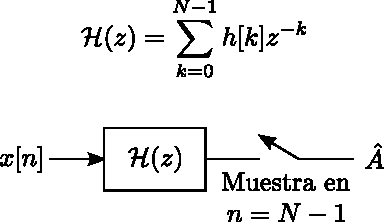
\includegraphics[width=\textwidth]{figuras/problem_6_11_fir_filter_estimator.pdf}
  \end{minipage}\hfill
  \begin{minipage}[c]{0.56\textwidth}
    \caption{
       Filtro FIR para estimar \(A\).
    } \label{fig:problem_6_11_fir_filter_estimator}
  \end{minipage}
\end{figure}

\paragraph{Solución} La restricción para que el filtro permita pasar el componente de continua incambiado es \(H(e^{j0})=1\), donde
\[
 H(e^{j2\pi f})=\sum_{k=-\infty}^{\infty}h[k]e^{-j2\pi fk}=\sum_{k=0}^{N-1}h[k]e^{-j2\pi fk}.
\]
Por lo tanto, evaluando en \(f=0\), la restricción es
\[
 H(e^{j0})=\sum_{k=0}^{N-1}h[k]=1,
\]
que en notación matricial puede escribirse como
\[
 \h^T\mathbf{1}=1,\qquad \textrm{con}\qquad \h=[h[0]\;h[1]\,\dots\,h[N-1]]^T
 \qquad\mathrm{y}\qquad \mathbf{1}=[1\;1\,\dots\,1]^T.
\]
Por otro lado, sea \(y[n]\) la salida del filtro. De esta forma,
\[
 y[n]=\sum_{k=0}^{N-1}h[k]x[n-k],
\]
y como el estimador de \(A\) es la muestra \(n=N-1\) de la salida del filtro,
\[
 \hat{A}=y[N-1]=\sum_{k=0}^{N-1}h[k]x[N-1-k].
\]
Como el filtro es lineal, la componente de la salida correspondiente al ruido en el instante \(n=N-1\) es
\[
 y_w[N-1]=\sum_{k=0}^{N-1}h[k]w[N-1-k],
\]
por lo que la potencia del ruido en ese instante es
\begin{align*}
 E(y_w^2[N-1])&=E\left[\left(\sum_{k=0}^{N-1}h[k]w[N-1-k]\right)^2\right]\\
  &=E\left(\sum_{k=0}^{N-1}h[k]w[N-1-k]\sum_{l=0}^{N-1}h[l]w[N-1-l]\right)\\
  &=\sum_{k=0}^{N-1}\sum_{l=0}^{N-1}h[k]h[l]E(w[N-1-k]w[N-1-l])\\
  &\overset{(a)}{=}\sum_{k=0}^{N-1}\sum_{l=0}^{N-1}h[k]h[l]r_{ww}[k-l]
\end{align*}
donde en \((a)\) se tuvo en cuenta que como el ruido es WSS, \(E(w[N-1-k]w[N-1-l])=E(w[k]w[l])=r_{ww}[k-l]\). La potencia del ruido puede por lo tanto expresarse en forma matricial como
\[
 E(y_w^2[N-1])=\h^T\C\h,
\]
donde \(\C\) es la matriz de covarianza de tamaño \(N\times N\) del ruido, con \(\C_{k,\,l}=r_{ww}[k-l]\), teniendo en cuenta que el ruido es de media nula. Finalmente, el problema de encontrar los coeficientes óptimos del filtro se puede formular como
\[
 \textrm{minimizar}\quad\h^T\C\h\quad\textrm{sujeto a}\quad\h^T\mathbf{1}=1.
\]
Se concluye que el problema es equivalente a encontrar el BLUE con \(\s=\textbf{1}\) (ver el apéndice 6A de \cite{kay93fundamentals}). Por lo tanto, el filtro óptimo es
\[
 \h_\textrm{opt}=\frac{\C^{-1}\mathbf{1}}{\mathbf{1}^T\C^{-1}\mathbf{1}}.
\]
Además, la potencia del ruido a la salida del filtro es
\[
  E(y_w^2[N-1])=\h_\textrm{opt}^T\C\h_\textrm{opt}=\frac{\mathbf{1}^T{\C^{-1}}^T\C\C^{-1}\mathbf{1}}{(\mathbf{1}^T\C^{-1}\mathbf{1})^2}
  =\frac{\mathbf{1}^T\C^{-1}\mathbf{1}}{(\mathbf{1}^T\C^{-1}\mathbf{1})^2}
  =\frac{1}{\mathbf{1}^T\C^{-1}\mathbf{1}}.
\]
En la estimación del nivel de DC en ruido WSS, el estimador BLUE puede verse como la salida de un filtro lineal que permite pasar incambiado el nivel de continua y cuyos coeficientes se eligen de forma de minimizar la potencia del ruido a la salida del filtro.

Como ejemplo, se considera el caso en que el ruido es un proceso WSS de media nula con ACF
\begin{equation}\label{eq:problem_6_11_noise_acf}
  r_{ww}[k]=
 \left\{
 \begin{array}{cl}
  1.81 &  k=0\\
  0 &  k=1\\
  r_{ww}[2] & k=2\\
  0 & k\geq 3
 \end{array}\right.,
\end{equation}
y el ruido contaminante es \(w_1[n]\) cuando \(r_{ww}[2]=0.9\) y \(w_2[n]\) cuando \(r_{ww}[2]=-0.9\). En ambos casos, la potencia del ruido es \(r_{ww}[0]=1.81\). La PSD se calculó en el problema de la sección \ref{sec:problem_6_10} y es
\[
 P_{ww}(f)=1.81+2r_{ww}[2]\cos4\pi f.
\]
Usando una computadora, se calcularon los coeficientes de filtro óptimo para los dos tipos de ruido usando \(N=10\) muestras. La PSD y la función de transferencia de los filtros óptimos, que son filtros FIR de orden \(N-1=9\), se muestran en la figura \ref{fig:problem_6_11}.
\begin{figure}[!htb]
\begin{center}
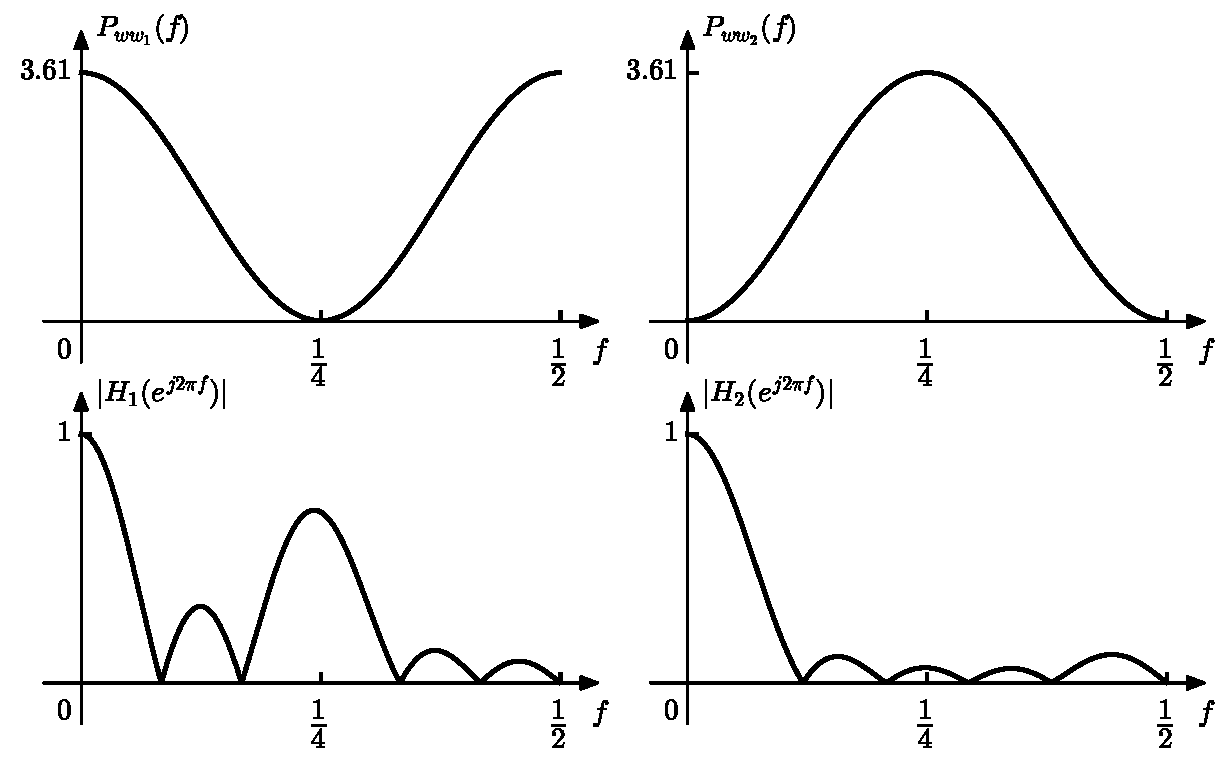
\includegraphics[width=0.9\textwidth]{figuras/problem_6_11.pdf}
\caption{\label{fig:problem_6_11} PSD del ruido y función de transferencia del filtro óptimo. \(P_{ww_1}(f)\) es la PSD del ruido cuando \(r_{ww}[2]=0.9\) y \(P_{ww_2}(f)\) es la PSD del ruido cuando \(r_{ww}[2]=-0.9\). \(H_1(e^{j2\pi f})\) y \(H_2(e^{j2\pi f})\) son las funciones de transferencia de los filtros óptimos de orden \(N-1=9\) en cada caso.}
\end{center}
\end{figure}
Como se observa en la figura, la potencia del ruido \(w_1[n]\) es máxima en torno a la continua y a la frecuencia máxima, mientras que la potencia del ruido \(w_2[n]\) es máxima en torno a la frecuencia \(f=1/2\) y nula en continua y el la frecuencia máxima. También se observa que el filtro óptimo, que debe tener ganancia unidad en continua, tiene menor ganancia en las frecuencias donde el ruido tiene mayor potencia. La potencia del ruido a la salida del filtro es en cada caso
\[
 E(y_{w_1}^2[N-1])\approx0.302\qquad\textrm{y}\qquad E(y_{w_2}^2[N-1])\approx0.028.
\]
Esto indica que el ruido \(w_2[n]\) es eliminado mas eficazmente, y se debe a que dicho ruido no tiene componentes espectrales en continua. El componente de continua no pueden ser eliminado debido a que es justamente es lo que se desea estimar. 

Para observar el desempeño del filtro óptimo en el dominio del tiempo, se generaron señales \(x[n]=A+w_{1,\,2}[n]\) con \(A=4\) y se filtraron con el filtro óptimo con \(N=50\). Los resultados se muestran en la figura \ref{fig:problem_6_11_sequences}. Se observa como el ruido \(w_2[n]\) es filtrado de forma mas eficaz que el ruido \(w_1[n]\).
\begin{figure}[!htb]
\begin{center}
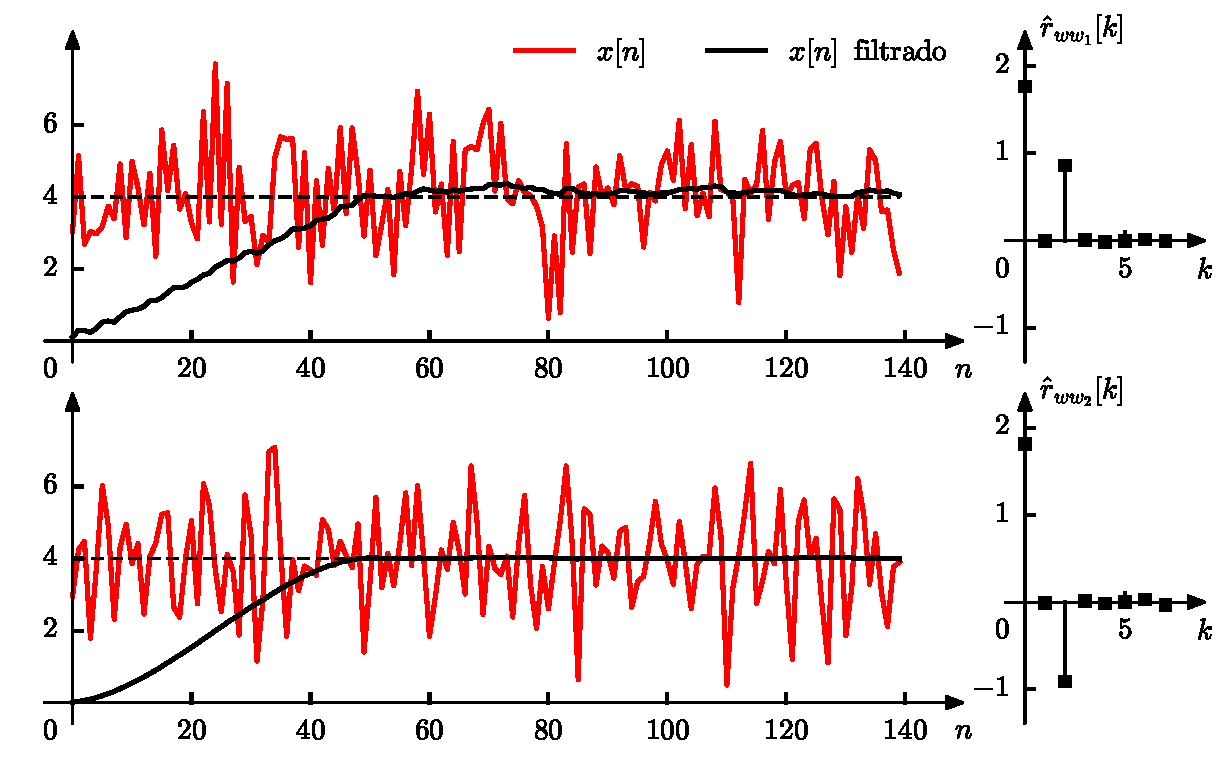
\includegraphics[width=0.9\textwidth]{figuras/problem_6_11_sequences.pdf}
\caption{\label{fig:problem_6_11_sequences} Nivel de DC \(x[n]=A+w_{1,\,2}[n]\) contaminado con ruido WSS y salida del filtro óptimo calculado con \(N=50\) muestras. El nivel de DC es \(A=4\). También se grafican las primeras muestras de la autocorrelación muestral \(\hat{r}_{ww_1}[k]\) y \(\hat{r}_{ww_2}[k]\) calculadas usando 10000 muestras del ruido \(w_1[n]\) y \(w_2[n]\) respectivamente.}
\end{center}
\end{figure}
Se realiza a continuación algunas observaciones sobre la generación de los ruidos \(w_{1,\,2}[n]\), que son procesos WSS dados por la ACF de la ecuación \ref{eq:problem_6_11_noise_acf}. Por tener autocorrelación de largo finito, se trata de procesos de media móvil (\emph{moving average}, MA), y pueden obtenerse mediante el filtrado de ruido blanco con un filtro FIR (ver el capítulo de \cite{hayes96statistical}), denominado filtro generador. Para encontrar los coeficientes de este filtro, se parte considerando que si se filtra un proceso \(v[n]\) con PSD \(P_{vv}(z)\) mediante un filtro con función de transferencia \(H_G(z)\), la PSD del proceso \(w[n]\) de salida es
\begin{equation}\label{eq:filtered_process_psd_z_domain}
 P_{ww}(z)=P_{vv}(z)H_G(z)H_G(1/z)
\end{equation}
si la respuesta al impulso \(h_G[n]\) del filtro es real. Si el proceso de entrada al filtro es ruido blanco de potencia \(\sigma_v^2\), su ACF es \(r_{vv}[k]=\sigma_v^2\delta[k]\) y su PSD es \(P_{vv}(z)=\sigma_v^2\). Además, el proceso \(w[n]\) que se quiere generar tiene en este caso ACF
\[
 r_{ww}[k]=r_{ww}[0]\delta[k]+r_{ww}[-2]\delta[k+2]+r_{ww}[2]\delta[k-2]
\]
y como \(r_{ww}[-2]=r_{ww}[2]\), su PSD es
\[
 P_{ww}(z)=r_{ww}[0]+r_{ww}[2]z^{-2}+r_{ww}[2]z^{2}.
\]
Para calcular \(H_G(z)\), se sustituye las PSD de \(v[n]\) y \(w[n]\) en la ecuación \ref{eq:filtered_process_psd_z_domain}, obteniendo que
\[
 r_{ww}[0]+r_{ww}[2]z^{-2}+r_{ww}[2]z^{2}=\sigma_v^2H(z)H(1/z),
\]
y por lo tanto,
\[
 H_G(z)H_G(1/z)=\frac{r_{ww}[0]+r_{ww}[2]z^{-2}+r_{ww}[2]z^{2}}{\sigma_v^2}.
\]
Se observa que esta ecuación se cumple con un filtro con transferencia de la forma \(H_G(z)=a+bz^{-2}\), ya que así
\[
 H_G(z)H_G(1/z)=(a+bz^{-2})(a+bz^{2})=a^2+abz^2+abz^{-2}+b^2
\]
e igualando con el lado derecho de la igualdad anterior, se tiene que
\[
\def\arraystretch{2.2}
 \left\{
 \begin{array}{ccc}
  a^2+b^2 & = & \dfrac{r_{ww}[0]}{\sigma_v^2}\\
  ab & = & \dfrac{r_{ww}[2]}{\sigma_v^2}
 \end{array}\right..
\]
Despejando \(b\) en la primera ecuación y sustituyendo en la primera, se obtiene que el coeficiente \(a\) cumple que
\[
 a^4\sigma_v^4-a^2\sigma_v^2r_{ww}[0]+r^2_{ww}[2]=0
 \qquad\qquad \textrm{o}\qquad\qquad x^2-xr_{ww}[0]+r^2_{ww}[2]=0,\qquad\textrm{con }a=\pm\frac{\sqrt{x}}{\sigma_v}.
\]
Por ejemplo, con los valores \(r_{ww}[0]=1.81\) y \(r_{ww}[2]=0.9\), los posibles valores \(a\) y \(b\) de los coeficientes del filtro generador son
\begin{center}
  \begin{tabular}{| c | c | c | c | c |}
    \hline
    \(\bm{a}\) & \(1\)   & \(-1\)   & \(0.9\)  & \(-0.9\) \\ \hline
    \(\bm{b}\) & \(0.9\) & \(-0.9\) &   \(1\)  &   \(-1\) \\ \hline
  \end{tabular}
\end{center}
Teniendo en cuenta que el filtro generador es de la forma \(H_G(z)=a+bz^{-2}\), los ruidos \(w_{1,\,2}[n]\) se generan con la ecuación en diferencias \(w[n]=av[n]+bv[n-2]\), donde \(v[n]\) es ruido blanco de potencia \(\sigma_v^2\). Para confirmar que los procesos generados efectivamente tienen la autocorrelación deseada, puede calcularse la autocorrelación muestral,
\[
 \hat{r}_{ww}[k]=\frac{1}{N-k}\sum_{n=0}^{N-1-k}x[n]x[n+k].
\]
Esto se hizo usando \(N=10000\) muestras de los ruidos generados y el resultado se muestra en la figura \ref{fig:problem_6_11_sequences}.

\subsection{Problema 12}\label{sec:problem_6_12}

Probar que el BLUE conmuta sobre transformaciones lineales (en realidad, afines) de \(\thetabf\). Es decir, si se quiere estimar
\[
 \alphabf=\B\thetabf+\bbf
\]
donde \(\B\) es una matriz conocida invertible \(p\times p\) y \(\bbf\) es un vector conocido \(p\times1\), probar que el BLUE está dado por
\[
 \hat{\alphabf}=\B\hat{\thetabf}+\bbf.
\]
donde \(\hat{\thetabf}\) es el BLUE para \(\thetabf\). Asumir que \(\x=\Hbf\thetabf+\w\), donde \(E(\w)=\mathbf{0}\) y \(E(\w\w^T)=\C\). Sugerencia: remplazar \(\thetabf\) por por \(\alphabf\) en el modelo de los datos.

\paragraph{Solución} Si el modelo de los datos es \(\x=\Hbf\thetabf+\w\), el estimador BLUE de \(\thetabf\) es (ver la ecuación \ref{eq:blue_estimator_vector})
\[
 \hat{\thetabf}=(\Hbf^T\C^{-1}\Hbf)^{-1}\Hbf^T\C^{-1}\x.
\]
Se quiere demostrar que el estimador del parámetro \(\alphabf\), que es la transformación afín de \(\thetabf\) dada por \(\alphabf=\B\thetabf+\bbf\), es \(\hat{\alphabf}=\B\hat{\thetabf}+\bbf\). Para hacerlo, se despeja \(\thetabf\) de la transformación,
\[
 \thetabf = \B^{-1}(\alphabf-\bbf),
\]
y se sustituye en el modelo de los datos,
\begin{align*}
 \x&=\Hbf\thetabf+\w\\
   &=\Hbf\B^{-1}(\alphabf-\bbf)+\w\\
   &=\Hbf\B^{-1}\alphabf-\Hbf\B^{-1}\bbf+\w,
\end{align*}
resultando en 
\[
 \x+\Hbf\B^{-1}\bbf=\Hbf\B^{-1}\alphabf+\w,
\]
que es el modelo lineal \(\x'=\Hbf'\alphabf+\w\) de parámetro \(\alphabf\) con \(\x'=\x+\Hbf\B^{-1}\bbf\) y \(\Hbf'=\Hbf\B^{-1}\). El estimador BLUE de \(\alphabf\) es por lo tanto
\begin{align*}
 \hat{\alphabf}&=\left(\Hbf'^T\C^{-1}\Hbf'\right)^{-1}\Hbf'^T\C^{-1}\x'\\
   &=\left({\B^{-1}}^T\Hbf^T\C^{-1}\Hbf\B^{-1}\right)^{-1}{\B^{-1}}^T\Hbf^T\C^{-1}\left(\x+\Hbf\B^{-1}\bbf\right)\\
   &=\B\left(\Hbf^T\C^{-1}\Hbf\right)^{-1}\B^T{\B^T}^{-1}\Hbf^T\C^{-1}\left(\x+\Hbf\B^{-1}\bbf\right)\\
   &=\B\left(\Hbf^T\C^{-1}\Hbf\right)^{-1}\Hbf^T\C^{-1}\x+
     \B\left(\Hbf^T\C^{-1}\Hbf\right)^{-1}\Hbf^T\C^{-1}\Hbf\B^{-1}\bbf\\
   &=\B\left(\Hbf^T\C^{-1}\Hbf\right)^{-1}\Hbf^T\C^{-1}\x+
     \B\B^{-1}\bbf\\
    &=\B\left(\Hbf^T\C^{-1}\Hbf\right)^{-1}\Hbf^T\C^{-1}\x+\bbf,
\end{align*}
donde se consideró que \({\B^{-1}}^T={\B^T}^{-1}\). Se concluye que el BLUE de \(\alphabf\)
es
\[
 \hat{\alphabf}=\B\hat{\thetabf}+\bbf,
\]
que es lo que se quería demostrar.

\subsection{Problema 13}\label{sec:problem_6_13}

En este problema se muestra que el BLUE es idéntico al \emph{estimador por mínimos cuadrados ponderados} que se discute en el capítulo 8. En particular, el estimador por mínimos cuadrados ponderados se obtiene minimizando la función
\[
 J=(\x-\Hbf\thetabf)^T\C^{-1}(\x-\Hbf\thetabf).
\]
Probar que el valor de \(\thetabf\) que minimiza \(J\) es el BLUE.

\paragraph{Solución} Desarrollando la función \(J\) se tiene que
\begin{align*}
  J&=(\x^T-\thetabf^T\Hbf^T)\C^{-1}(\x-\Hbf\thetabf)\\
   &=\x^T\C^{-1}\x-2\x^T\C^{-1}\Hbf\thetabf+\thetabf^T\Hbf^T\C^{-1}\Hbf\thetabf,
\end{align*}
y la derivada respecto al parámetro es
\[
 \frac{\partial J}{\partial\thetabf}=-2\Hbf^T\C^{-1}\x+2\Hbf^T\C^{-1}\Hbf\thetabf,
\]
donde se emplearon los resultados deducidos en el apéndice \ref{ap:derivatives_respect_vector} que indican que
\[
 \frac{\partial \mathbf{b}^T\thetabf}{\partial\thetabf}=\mathbf{b},
 \qquad\qquad\frac{\partial \thetabf^T\mathbf{A}\thetabf}{\partial\thetabf}=2\mathbf{A}\thetabf.
\]
Finalmente, igualando la derivada a cero,
\[
 \Hbf^T\C^{-1}\Hbf\hat{\thetabf}=\Hbf^T\C^{-1}\x
\]
y despejando el parámetro, se obtiene que el valor que minimiza \(J\) es
\[
 \hat{\thetabf}=(\Hbf^T\C^{-1}\Hbf)^{-1}\Hbf^T\C^{-1}\x,
\]
que es el BLUE.

\subsection{Problema 14}\label{sec:problem_6_14}

Un proceso ruidoso se compone de variables aleatorias IID de media nula con PDF
\[
 p(w[n])=\frac{1-\epsilon}{\sqrt{2\pi\sigma^2_B}}\exp\left[-\frac{1}{2}\left(\frac{w^2[n]}{\sigma^2_B}\right)\right]+
 \frac{\epsilon}{\sqrt{2\pi\sigma^2_I}}\exp\left[-\frac{1}{2}\left(\frac{w^2[n]}{\sigma^2_I}\right)\right],
\]
donde \(0<\epsilon<1\). Dicha PDF se denomina \emph{mezcla gaussiana}. Se emplea para modelar ruido que es gaussiano de varianza \(\sigma^2_B\) el \(100(1-\epsilon)\%\) del tiempo y gaussiano de varianza \(\sigma^2_I\) el resto del tiempo. Típicamente, \(\sigma^2_I\gg\sigma^2_B\) y \(\epsilon\ll1\), de forma que el ruido predominante es ruido de fondo con varianza \(\sigma^2_B\) pequeña pero también contiene ocasionalmente ruido de alta potencia o interferencias modeladas como ruido gaussiano de varianza \(\sigma^2_I\) grande. Mostrar que la varianza de esta PDF es
\[
 \sigma^2=(1-\epsilon)\sigma^2_B+\epsilon\sigma^2_I.
\]
Si los datos son \(\{w^2[0],\,\dots,\,w^2[N-1]\}\) y \(\sigma^2_B\) y \(\epsilon\) se asumen conocidos, encontrar el BLUE de \(\sigma^2_I\). Sugerencia: emplear los resultados del problema de la sección \ref{sec:problem_6_12}.

\paragraph{Solución} Para calcular la varianza de \(w[n]\) se parte observando que \(E(w[n])=0\), ya que \(w[n]\sim(1-\epsilon)\mathcal{N}(0,\,\sigma^2_B)+\epsilon\mathcal{N}(0,\,\sigma^2_I)\). Por lo tanto, la varianza es
\begin{align*}
 \var(w[n])&=E(w^2[n])\\
  &=\int_{-\infty}^{\infty}w^2[n]p(w[n])\,dw[n]\\
  &=\int_{-\infty}^{\infty}w^2[n]\left\{\frac{1-\epsilon}{\sqrt{2\pi\sigma^2_B}}\exp\left[-\frac{1}{2}\left(\frac{w^2[n]}{\sigma^2_B}\right)\right]+
 \frac{\epsilon}{\sqrt{2\pi\sigma^2_I}}\exp\left[-\frac{1}{2}\left(\frac{w^2[n]}{\sigma^2_I}\right)\right]\right\}\,dw[n]\\
 &=(1-\epsilon)\int_{-\infty}^{\infty}w^2[n]\frac{1}{\sqrt{2\pi\sigma^2_B}}\exp\left[-\frac{1}{2}\left(\frac{w^2[n]}{\sigma^2_B}\right)\right]\,dw[n]\\
 &\qquad+\epsilon\int_{-\infty}^{\infty}w^2[n]\frac{1}{\sqrt{2\pi\sigma^2_I}}\exp\left[-\frac{1}{2}\left(\frac{w^2[n]}{\sigma^2_I}\right)\right]\,dw[n]\\
 &\overset{(a)}{=}(1-\epsilon)\sigma^2_B+\epsilon\sigma^2_I,
\end{align*}
donde en \((a)\) se consideró que la primer integral es la varianza de una variable aleatoria \(\mathcal{N}(0,\,\sigma^2_B)\) y la segunda integral es la varianza de una variable aleatoria \(\mathcal{N}(0,\,\sigma^2_I)\).

Se calculará a continuación el BLUE de \(\sigma_I^2\). Teniendo en cuenta que los datos son \(\{w^2[0],\,\dots,\,w^2[N-1]\}\), se considera la transformación \(y[n]=w^2[n]\). De esta forma, se cumple que \(E(y[n])=\sigma^2\). Además, las muestras \(y[n]\) son IID por ser las muestras \(w[n]\) IID y por lo tanto, la matriz de covarianza del vector de las muestras \(y[n]\) es \(\C=\var(y[n])\I\). Los datos transformados se pueden expresar como
\begin{align*}
 y[n]&=E(y[n])+(y[n]-E(y[n]))\\
  &=\sigma^2+v[n]
\end{align*}
o en notación matricial como
\[
 \y=\mathbf{1}\sigma^2+\vbf,
\]
donde el ruido \(\vbf\) cumple que \(E(\vbf)=\mathbf{0}\) y tiene matriz de covarianza la matriz de covarianza de \(\y\). Por lo tanto, el BLUE de \(\sigma^2\) esta dado por la ecuación \ref{eq:blue_estimator_scalar} con \(\s=\mathbf{1}\) y es
\[
 \hat{\sigma}^2=\frac{\mathbf{1}^T\C^{-1}\y}{\mathbf{1}^T\C^{-1}\mathbf{1}}
  =\frac{\mathbf{1}^T\left(\dfrac{1}{\var(y[n])}\I\right)\y}{\mathbf{1}^T\left(\dfrac{1}{\var(y[n])}\I\right)\mathbf{1}}
  =\frac{\mathbf{1}^T\y}{\mathbf{1}^T\mathbf{1}}
  =\frac{1}{N}\sum_{n-0}^{N-1}y[n],
\]
es decir,
\[
 \hat{\sigma^2}=\frac{1}{N}\sum_{n-0}^{N-1}w^2[n].
\]
Además, como
\[
 \sigma^2=(1-\epsilon)\sigma^2_B+\epsilon\sigma^2_I
\]
se cumple que
\[
 \sigma^2_I=\frac{\sigma^2-(1-\epsilon)\sigma^2_B}{\epsilon}.
\]
En el problema de la sección \ref{sec:problem_6_12} se dedujo que el BLUE se mantiene en trasformaciones afines del parámetro y por lo tanto, el BLUE de \(\sigma^2_I\) es
\[
 \hat{\sigma^2_I}=\frac{\hat{\sigma}^2-(1-\epsilon)\sigma^2_B}{\epsilon}
\]
resultando en
\[
 \hat{\sigma^2_I}=\frac{\displaystyle\frac{1}{N}\sum_{n-0}^{N-1}w^2[n]-(1-\epsilon)\sigma^2_B}{\epsilon}.
\]

\subsection{Problema 15}

Para el modelo lineal general
\[
 \x=\Hbf\thetabf+\s+\w
\]
donde \(\s\) es un vector \(N\times1\) conocido y \(E(\w)=0\), \(E(\w\w^T)=\C\), encontrar el BLUE. 

\paragraph{Solución} Definiendo \(\x'=\x-\s\) el modelo de los datos se puede expresar como
\[
 \x'=\Hbf\thetabf+\w,
\]
que es el modelo lineal habitual. De la ecuación \ref{eq:blue_estimator_vector}, el BLUE es
\[
 \hat{\thetabf}=(\Hbf^T\C^{-1}\Hbf)^{-1}\Hbf^T\C^{-1}\x',
\]
resultando en
\[
 \hat{\thetabf}=(\Hbf^T\C^{-1}\Hbf)^{-1}\Hbf^T\C^{-1}(\x-\s).
\]

\subsection{Problema 16}

En la implementación del BLUE para el modelo lineal descripto en el teorema de Gauss-Markov (sección \ref{sec:blue_gauss_markov}), es posible usar sin saberlo una matriz de covarianza errónea para formar el estimador
\[
  \hat{\thetabf}=(\Hbf^T\hat{\C}^{-1}\Hbf)^{-1}\Hbf^T\hat{\C}^{-1}\x.
\]
Para examinar el efecto de este error de modelado, asúmase que se quiere estimar el nivel de continua \(A\) en WGN en ruido no correlacionado. Calcular la varianza de este estimador y la varianza del estimador BLUE para el caso en que \(N=2\) y
\[
 \C=
  \begin{bmatrix}
  1 & 0\\
  0 & 1
  \end{bmatrix}
  \qquad\qquad\textrm{y}\qquad\qquad
  \hat{\C}=
  \begin{bmatrix}
  1 & 0\\
  0 & \alpha
  \end{bmatrix}.
\]
Comparar las varianzas cuando \(\alpha\to0\), \(\alpha=1\) y \(\alpha\to\infty\),

\paragraph{Solución} El modelo de los datos es
\[
 \x=\mathbf{1}A+\w,
\]
y \(\w\) tiene matriz de covarianza \(\C\). La varianza del estimador BLUE 
\[
 \var_\textrm{BLUE}(\hat{A})=\frac{1}{\mathbf{1}^T\C^{-1}\mathbf{1}}=\frac{1}{2},
\]
ya que \(\mathbf{1}^T\C^{-1}\mathbf{1}\) es la suma de todos los elementos de \(\C\). Para calcular la varianza del estimador empleando un modelo erróneo, se parte calculando la media del estimador. El estimador es
\[
 \hat{A}=\frac{\mathbf{1}^T\hat{\C}^{-1}\mathbf{\x}}{\mathbf{1}^T\hat{\C}^{-1}\mathbf{1}},
\]
por lo que su media es
\begin{align*}
 E(\hat{A})&=\frac{\mathbf{1}^T\hat{\C}^{-1}E(\mathbf{\x})}{\mathbf{1}^T\hat{\C}^{-1}\mathbf{1}}\\
  &=\frac{\mathbf{1}^T\hat{\C}^{-1}\mathbf{1}A}{\mathbf{1}^T\hat{\C}^{-1}\mathbf{1}}\\
  &=A.
\end{align*}
Por lo tanto, el estimador es insesgado independientemente de la matriz \(\hat{\C}\). La varianza del estimador es
\begin{align*}
 \var(\hat{A})&=E\left[(\hat{A}-A)^2\right]\\
  &=E\left[\left(\frac{\mathbf{1}^T\hat{\C}^{-1}E(\mathbf{\x})}{\mathbf{1}^T\hat{\C}^{-1}\mathbf{1}}-A\right)^2\right]\\
  &=E\left[\left(\frac{\mathbf{1}^T\hat{\C}^{-1}E(\mathbf{\x})-\mathbf{1}^T\hat{\C}^{-1}\mathbf{1}A}{\mathbf{1}^T\hat{\C}^{-1}\mathbf{1}}\right)^2\right]\\
  &=E\left\{\left[\frac{\mathbf{1}^T\hat{\C}^{-1}\left(E(\mathbf{\x})-A\right)}{\mathbf{1}^T\hat{\C}^{-1}\mathbf{1}}\right]^2\right\}\\
  &=E\left[\left(\frac{\mathbf{1}^T\hat{\C}^{-1}\w}{\mathbf{1}^T\hat{\C}^{-1}\mathbf{1}}\right)^2\right]\\
  &=E\left[\frac{\mathbf{1}^T\hat{\C}^{-1}\w\w^T\hat{\C}^{-1}\mathbf{1}}{\left(\mathbf{1}^T\hat{\C}^{-1}\mathbf{1}\right)^2}\right]\\
  &=\frac{\mathbf{1}^T\hat{\C}^{-1}E(\w\w^T)\hat{\C}^{-1}\mathbf{1}}{\left(\mathbf{1}^T\hat{\C}^{-1}\mathbf{1}\right)^2},
\end{align*}
concluyendo que
\[
 \var(\hat{A})=\frac{\mathbf{1}^T\hat{\C}^{-1}\C\hat{\C}^{-1}\mathbf{1}}{\left(\mathbf{1}^T\hat{\C}^{-1}\mathbf{1}\right)^2}.
\]
Sustituyendo los valores de las matrices \(\C\) y \(\hat{\C}\), teniendo en cuenta que
\[
 \hat{\C}^{-1}\C\hat{\C}^{-1}=\hat{\C}^{-1}\I\hat{\C}^{-1}=
 \hat{\C}^{-1}\hat{\C}^{-1}=
 \begin{bmatrix}
  1 & 0\\
  0 & \dfrac{1}{\alpha}
  \end{bmatrix}
  \begin{bmatrix}
  1 & 0\\
  0 & \dfrac{1}{\alpha}
  \end{bmatrix}=
  \begin{bmatrix}
  1 & 0\\
  0 & \dfrac{1}{\alpha^2}
  \end{bmatrix},
\]
se obtiene que
\[
 \var(\hat{A})=\frac{1+\dfrac{1}{\alpha^2}}{\left(1+\dfrac{1}{\alpha}\right)^2}
 =\frac{\alpha^2+1}{(\alpha+1)^2}.
\]
Por lo tanto, se cumple que
\[
 \var(\hat{A})=\frac{\alpha^2+1}{(\alpha+1)^2}=
 \left\{
 \begin{array}{ccl}
  1 & \textrm{si} & \alpha\to0\\
  \dfrac{1}{2} & \textrm{si} & \alpha=1\\
  1 & \textrm{si} & \alpha\to\infty
 \end{array}\right..
\]
Cuando \(\alpha=1\), se obtiene el BLUE, que es el estimador lineal insesgado con menor varianza. En la figura \ref{fig:problem_6_16} se muestra la varianza del estimador en función de \(\alpha\).
\begin{figure}[!htb]
  \begin{minipage}[c]{0.55\textwidth}
    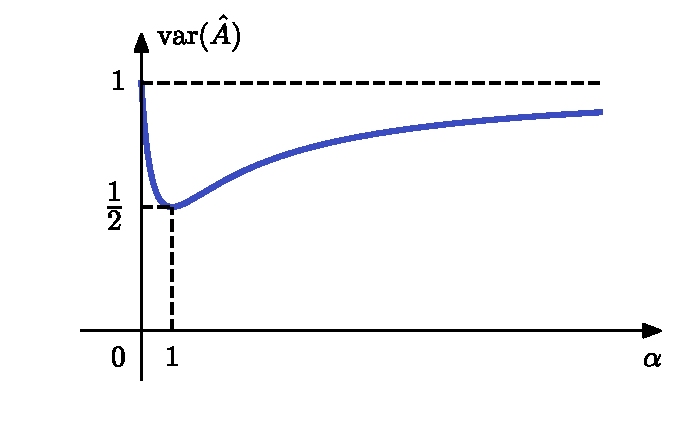
\includegraphics[width=\textwidth]{figuras/problem_6_16.pdf}
  \end{minipage}\hfill
  \begin{minipage}[c]{0.35\textwidth}
    \caption{
       Varianza del estimador con modelado erróneo.
    } \label{fig:problem_6_16}
  \end{minipage}
\end{figure}

\chapter{Estimación de máxima verosimilitud}\label{ch:mle}

\section{Estimador de máxima verosimilitud}

\subsection{Definición}

El estimador de máxima verosimilitud (\emph{maximum likelihood estimator}, MLE) se define como el valor del parámetro \(\theta\) que maximiza \(p(\x;\,\theta)\) para \(\x\) fijo, es decir, el valor que maximiza la función de verosimilitud.

\subsection{Propiedades asintóticas del MLE}\label{sec:mle_asintotic_properties}

\paragraph{Teorema} Si la PDF \(p(\x;\,\theta)\) de los datos \(\x\) satisface ciertas condiciones de regularidad, el estimador MLE del parámetro desconocido \(\theta\) es asintóticamente distribuido como
\[
 \hat{\theta}\overset{a}{\sim}\mathcal{N}(\theta,\,I^{-1}(\theta))
\]
donde \(I(\theta)\) es la información de Fisher evaluada en el valor verdadero del parámetro desconocido. 

En la demostración, para la cual se emplea la ley de los grandes números y el teorema central del límite, se especifican las condiciones de regularidad y los modos de convergencia del estimador MLE. Una introducción a los tipos de convergencia y teoremas sobre límites de secuencias de variables aleatorias puede encontrarse por ejemplo en el capítulo 7 de \cite{papoulis2002probability}.

\paragraph{Demostración} Se incluye a continuación una demostración poco rigurosa cuyo objetivo es ilustrar las ideas principales. Además, para simplificar la discusión, se asume que las observaciones son IID. Las condiciones de regularidad que tiene que cumplir la función de verosimilitud son las siguientes:
\begin{enumerate}
 \item Las derivadas primera y segunda de la función de verosimilitud logarítmica están bien definidas.
 \item 
 \[
  E\left[\frac{\partial\ln p(x[n];\,\theta)}{\partial\theta}\right]=0.
 \]
 Esta es la misma condición de regularidad que la del teorema de CRLB.
\end{enumerate}

Primero se demostrará que el MLE \(\hat{\theta}\) es consistente. Esto significa que si \(\theta_0\) es el valor verdadero del parámetro, \(\hat{\theta}\to\theta_0\) en probabilidad cuando \(N\to\infty\). Para hacerlo, se necesitará la divergencia de Kullback-Leiber\footnote{Ver por ejemplo \href{https://en.wikipedia.org/wiki/Kullback\%E2\%80\%93Leibler_divergence}{https://en.wikipedia.org/wiki/Kullback-Leibler\_divergence}.}, que indica que
\begin{equation}\label{eq:kullback_leiber_divergence}
 \int \ln\left[\frac{p(x)}{q(x)}\right]p(x)\,dx\geq0,
\end{equation}
donde \(p(x)\) y \(q(x)\) son densidades de probabilidad, y la igualdad se da si y solo si \(q(x)=p(x)\). Para probar esta desigualdad, se observa que la formulación
\[
 \int \ln\left[\frac{q(x)}{p(x)}\right]p(x)\,dx\leq 0
\]
es equivalente, y partiendo del lado izquierdo de esta última expresión, se ve que
\begin{align*}
 \int \ln\left[\frac{q(x)}{p(x)}\right]p(x)\,dx
  &\overset{(a)}{\leq}\int \left[\frac{q(x)}{p(x)}-1\right]p(x)\,dx\\
  &=\int q(x)\,dx-\int p(x)\,dx\\
  &=1-1\\
  &=0,
\end{align*}
donde en \((a)\) se empleó que \(\ln x\leq x-1\) para todo \(x>0\). La igualdad se da cuando \(\ln x = x-1\), es decir, en \(x=1\), que implica que \(q(x)=p(x)\). Maximizar la función de verosimilitud logarítmica es equivalente a maximizar
\begin{align*}
 \frac{1}{N}\ln p(\x;\,\theta)&=\frac{1}{N}\ln\prod_{n=0}^{N-1}p(x[n];\,\theta)\\
  &=\frac{1}{N}\sum_{n=0}^{N-1}\ln p(x[n];\,\theta).
\end{align*}
Cuando \(N\to\infty\), por la ley de los grandes números, esto converge en probabilidad al valor esperado. Por lo tanto, 
\begin{equation}\label{eq:mle_consistency_dem}
 \frac{1}{N}\sum_{n=0}^{N-1}\ln p(x[n];\,\theta)\overset{p}{\longrightarrow}E[\ln p(x[n];\,\theta)]=\int \ln p(x[n];\,\theta)p(x[n];\,\theta_0)\,dx[n],
\end{equation}
donde \(\theta_0\) es el valor verdadero del parámetro. Considerando la divergencia de Kullback-Leiber de la ecuación \ref{eq:kullback_leiber_divergence}, se cumple que
\[
 \int\ln\left[\frac{p(x[n];\,\theta_1)}{p(x[n];\,\theta_2)}\right]p(x[n];\,\theta_1)\,dx[n]\geq 0, 
\]
es decir,
\[
 \int\ln p(x[n];\,\theta_1)p(x[n];\,\theta_1)\,dx[n]\geq
   \int\ln p(x[n];\,\theta_2)p(x[n];\,\theta_1)\,dx[n].
\]
Esto indica que el lado derecho de la ecuación \ref{eq:mle_consistency_dem} es maximizado para \(\theta=\theta_0\). Por lo tanto, asumiendo condiciones de continuidad apropiadas, el lado izquierdo de la ecuación \ref{eq:mle_consistency_dem} también es maximizado para \(\theta=\theta_0\). Como por definición el MLE \(\hat{\theta}\) maximiza el lado izquierdo \ref{eq:mle_consistency_dem}, se cumple que cuando \(N\to\infty\), el MLE es \(\hat{\theta}=\theta_0\). Se concluye que el MLE es consistente.

Se deriva a continuación la PDF asintótica del MLE, que cumple que
\[
 \hat{\theta}\overset{d}{\longrightarrow}\mathcal{N}(\theta_0,\,I^{-1}(\theta_0)),
\]
es decir, el estimador converge a una distribución normal de media \(\theta_0\) y varianza \(I^{-1}(\theta_0)\). Para demostrarlo, se parte considerando el teorema del valor medio\footnote{Ver \url{https://en.wikipedia.org/wiki/Mean\_value\_theorem}.}, que indica que bajo las hipótesis adecuadas se cumple que
\[
  f'(c)=\frac{f(b)-f(a)}{b-a}, \qquad\textrm{o}\qquad
  f(b)=f(a)+f'(c)(b-a)\qquad\textrm{para }a<c<b.
\]
Aplicando el teorema del valor medio a 
\[
 f(\theta)=\dfrac{\partial\ln p(\x;\,\theta)}{\partial\theta}\qquad
 \textrm{con}\qquad a=\theta_0,\quad b=\hat{\theta},
\]
se cumple que 
\[
 \frac{\partial\ln p(\x;\,\theta)}{\partial\theta}\bigg|_{\theta=\hat{\theta}}=
 \frac{\partial\ln p(\x;\,\theta)}{\partial\theta}\bigg|_{\theta=\theta_0}+
 \frac{\partial^2\ln p(\x;\,\theta)}{\partial\theta^2}\bigg|_{\theta=\tilde{\theta}}(\hat{\theta}-\theta_0)
\]
para algún \(\tilde{\theta}\) tal que \(\theta_0<\tilde{\theta}<\hat{\theta}\). Pero por definición del MLE,
\[
 \frac{\partial\ln p(\x;\,\theta)}{\partial\theta}\bigg|_{\theta=\hat{\theta}}=0
\]
y por lo tanto,
\[
 0=
 \frac{\partial\ln p(\x;\,\theta)}{\partial\theta}\bigg|_{\theta=\theta_0}+
 \frac{\partial^2\ln p(\x;\,\theta)}{\partial\theta^2}\bigg|_{\theta=\tilde{\theta}}(\hat{\theta}-\theta_0).
\]
Despejando \(\hat{\theta}-\theta_0\) y multiplicando ambos lados de la igualdad por \(\sqrt{N}\), se tiene que
\[
 \sqrt{N}(\hat{\theta}-\theta_0)=
 -\frac{\sqrt{N}\dfrac{\partial\ln p(\x;\,\theta)}{\partial\theta}\bigg|_{\theta=\theta_0}}{\dfrac{\partial^2\ln p(\x;\,\theta)}{\partial\theta^2}\bigg|_{\theta=\tilde{\theta}}}
\]
y dividiendo el numerador y el denominador entre \(N\) se llega a que
\begin{equation}\label{eq:mle_asymptotic_pdf_dem}
 \sqrt{N}(\hat{\theta}-\theta_0)=
 \frac{\dfrac{1}{\sqrt{N}}\dfrac{\partial\ln p(\x;\,\theta)}{\partial\theta}\bigg|_{\theta=\theta_0}}{-\dfrac{1}{N}\dfrac{\partial^2\ln p(\x;\,\theta)}{\partial\theta^2}\bigg|_{\theta=\tilde{\theta}}}.
\end{equation}
Se considera ahora el denominador de la ecuación \ref{eq:mle_asymptotic_pdf_dem}. Como los datos son IID, se cumple que
\[
 \frac{1}{N}\frac{\partial^2\ln p(\x;\,\theta)}{\partial\theta^2}\bigg|_{\theta=\tilde{\theta}}=
 \frac{1}{N}\sum_{n=0}^{N-1}\frac{\partial^2\ln p(x[n];\,\theta)}{\partial\theta^2}\bigg|_{\theta=\tilde{\theta}}.
\]
Como \(\theta_0<\tilde{\theta}<\hat{\theta}\), se cumple que \(\tilde{\theta}\to\theta_0\) con \(N\to\infty\) debido a la consistencia del MLE. Por lo tanto,
\begin{align*}
 \frac{1}{N}\frac{\partial^2\ln p(\x;\,\theta)}{\partial\theta^2}\bigg|_{\theta=\tilde{\theta}}
 &\to\frac{1}{N}\sum_{n=0}^{N-1}\frac{\partial^2\ln p(x[n];\,\theta)}{\partial\theta^2}\bigg|_{\theta=\theta_0}\\
 &\overset{(a)}{\to} E\left[\frac{\partial^2\ln p(x[n];\,\theta)}{\partial\theta^2}\bigg|_{\theta=\theta_0}\right]\\
 &=-i(\theta_0).
\end{align*}
donde la convergencia en \((a)\) es probabilidad por la ley de los grandes números. \(i(\theta_0)\) es la información de Fisher de una muestra. Empleando nuevamente la hipótesis de IID, el numerador de la ecuación \ref{eq:mle_asymptotic_pdf_dem} es
\[
 \frac{1}{\sqrt{N}}\frac{\partial\ln p(\x;\,\theta)}{\partial\theta}\bigg|_{\theta=\theta_0}=
 \frac{1}{\sqrt{N}}\sum_{n=0}^{N-1}\frac{\partial\ln p(x[n];\,\theta)}{\partial\theta}\bigg|_{\theta=\theta_0}.
\]
Se observa que
\[
 \xi_n=\frac{\partial \ln p(x[n];\,\theta)}{\partial \theta}\bigg|_{\theta=\theta_0}
\]
es una variable aleatoria por ser una función de \(x[n]\). Además, como los \(x[n]\) son IID, también los son los \(\xi_n\). Por lo tanto, por el teorema central del límite, el numerador de la ecuación \ref{eq:mle_asymptotic_pdf_dem} tiene una PDF que converge a una PDF gaussiana. La media de esta PDF gaussiana es
\begin{align*}
 E\left[\frac{1}{\sqrt{N}}\sum_{n=0}^{N-1}\frac{\partial\ln p(x[n];\,\theta)}{\partial\theta}\bigg|_{\theta=\theta_0}\right]
 &=\frac{1}{\sqrt{N}}\sum_{n=0}^{N-1}E\left[\frac{\partial\ln p(x[n];\,\theta)}{\partial\theta}\bigg|_{\theta=\theta_0}\right]\\
 &\overset{(a)}{=}\frac{1}{\sqrt{N}}\sum_{n=0}^{N-1}\frac{\partial E[\ln p(x[n];\,\theta)]}{\partial\theta}\bigg|_{\theta=\theta_0}\\
 &\overset{(b)}{=}0,
\end{align*}
donde en \((a)\) se intercambió el orden de diferenciación y esperanza, lo cual es posible gracias a la condición de regularidad del punto 2., como se mostró en la sección \ref{sec:crlb_scalar}, y en \((b)\) se tuvo en cuenta que el término \(E[\ln p(x[n];\,\theta)]\) está dado por la integral de la ecuación \ref{eq:mle_consistency_dem}, la cual es una función de \(\theta\) que es máxima cuando \(\theta=\theta_0\), por lo que su derivada respecto a \(\theta\) evaluada en el máximo \(\theta_0\) debe ser nula. Además, la varianza es
\begin{align*}
 E\left[\left(\frac{1}{\sqrt{N}}\sum_{n=0}^{N-1}\frac{\partial\ln p(x[n];\,\theta)}{\partial\theta}\bigg|_{\theta=\theta_0}\right)^2\right]
  &\overset{(a)}{=}\frac{1}{N}\sum_{n=0}^{N-1}E\left[\left(\frac{\partial\ln p(x[n];\,\theta)}{\partial\theta}\right)^2\bigg|_{\theta=\theta_0}\right]\\
  &\overset{(b)}{=}\frac{1}{N}Ni(\theta_0)\\
  &=i(\theta_0),
\end{align*}
donde en \((a)\) se consideró que las variables aleatorias \(\xi_n\) son IID y de media nula y en \((b)\) se empleó la expresión alternativa de la información de Fisher dada por la ecuación  \ref{eq:crlb_second_derivative_expectation}. Para continuar la deducción, hay que referirse al teorema de Slutsky\footnote{Ver por ejemplo \href{https://en.wikipedia.org/wiki/Slutsky\%27s_theorem}{https://en.wikipedia.org/wiki/Slutsky's\_theorem}.}, que indica que si la secuencia de variables aleatorias \(x_n\) converge en distribución a la variable aleatoria \(x\) y la secuencia de variables aleatorias \(y_n\) converge en probabilidad a una constante \(c\), se cumple que \(x_n/y_n\) converge en distribución a la variable aleatoria \(x/c\). En el caso de la ecuación \ref{eq:mle_asymptotic_pdf_dem}, se vió que el numerador y el denominador convergen respectivamente a
\[
 x_n\overset{d}{\longrightarrow}x\sim\mathcal{N}(0,\,i(\theta_0)),\qquad\qquad y_n\overset{p}{\longrightarrow}c=i(\theta_0),
\]
y por lo tanto, como
\[
 \var\left(\frac{x}{c}\right)=\frac{\var(x)}{c^2}=\frac{i(\theta_0)}{i^2(\theta_0)}=i^{-1}(\theta_0),
\]
la ecuación \ref{eq:mle_asymptotic_pdf_dem} converge asintóticamente a
\[
 \sqrt{N}(\hat{\theta}-\theta_0)\overset{a}{\sim}\mathcal{N}(0,\,i^{-1}(\theta_0)),
\]
o equivalentemente
\[
 \hat{\theta}\overset{a}{\sim}\mathcal{N}\left(\theta_0,\,\frac{1}{Ni(\theta_0)}\right),
\]
y finalmente
\[
 \hat{\theta}\overset{a}{\sim}\mathcal{N}\left(\theta_0,\,I^{-1}(\theta_0)\right),
\]
donde en esta última ecuación se tuvo en cuenta que como los datos son IID, la información de Fisher \(I(\theta_0)\) de los datos es la suma de la información de Fisher \(i(\theta_0)\) de cada muestra.

\subsection{Propiedad de invarianza del MLE}\label{sec:mle_invariance_property}

\paragraph{Teorema: propiedad de invarianza del MLE.} El MLE del parámetro \(\alpha=g(\theta)\), donde la PDF \(p(\x,\,\theta)\) es parametrizada por \(\theta\), está dada por
\[
 \hat{\alpha}=g(\hat{\theta})
\]
donde \(\hat{\theta}\) es el MLE de \(\theta\). El MLE de \(\hat{\theta}\) se obtiene maximizando \(p(\x,\,\theta)\). Si \(g\) no es una función uno a uno (inyectiva), \(\hat{\alpha}\) maximiza la función de verosimilitud modificada \(\bar{p}_T(\x,\,\alpha)\), definida como
\[
 \bar{p}_T(\x,\,\alpha)=\max_{\{\theta:\,\alpha=g(\theta)\}}p(\x;\,\theta).
\]


\subsection{MLE para el modelo lineal}\label{sec:mle_linear_model}

\paragraph{Teorema: optimalidad del MLE para el modelo lineal.} Si los datos observados \(\x\) son descriptos por el modelo lineal general (ecuación \ref{eq:linear_model})
\[
 \x=\Hbf\thetabf+\w
\]
donde \(\Hbf\) es una matriz \(N\times p\) conocida con \(N>p\) y rango \(p\), \(\thetabf\) es un vector \(p\times1\) de parámetros a estimar y \(\w\) es un vector de ruido \(N\times1\) con PDF \(\mathcal{N}(\mathbf{0},\,\C)\), el MLE de \(\thetabf\) es
\begin{equation}\label{eq:mle_linear_model_estimator}
 \hat{\thetabf}=(\Hbf^T\C^{-1}\Hbf)^{-1}\Hbf^T\C^{-1}\x.
\end{equation}
\(\hat{\thetabf}\) es además un estimador eficiente ya que alcanza la CRLB y por lo tanto, es el estimador MVU. La PDF de \(\hat{\thetabf}\) es
\[
 \hat{\thetabf}\sim\mathcal{N}(\thetabf,\,(\Hbf^T\C^{-1}\Hbf)^{-1}).
\]
Este resultado puede generalizarse mediante la afirmación de que si existe un estimador eficiente, está dado por el MLE, como se muestra en el problema de la sección \ref{sec:problem_7_12}.

\paragraph{Demostración.} Para el modelo lineal general, la PDF de los datos es
\[
 p(\x;\,\thetabf)=\frac{1}{(2\pi)^\frac{N}{2}\det^\frac{1}{2}(\C)}\exp\left[-\frac{1}{2}(\x-\Hbf\thetabf)^T\C^{-1}(\x-\Hbf\thetabf)\right]
\]
por lo que el MLE se obtiene minimizando 
\begin{equation}\label{eq:mle_linear_model_j}
 J(\thetabf)=(\x-\Hbf\thetabf)^T\C^{-1}(\x-\Hbf\thetabf),
\end{equation}
y como es una función cuadrática en los elementos de \(\thetabf\) y \(\C^{-1}\) es una matriz definida positiva, la diferenciación produce el mínimo global. En la sección \ref{sec:crlb_general_gaussian} sobre la CRLB para el caso gaussiano general, se demostró que si \(\x\sim\mathcal{N}(\mubf(\thetabf),\, \C(\thetabf))\), 
\[
 \frac{\partial\ln p(\x;\,\thetabf)}{\partial\theta_k}=-\frac{1}{2}\tr\left(\C^{-1}(\thetabf)\frac{\partial\C(\thetabf)}{\partial\theta_k}\right)+\frac{\partial\bm{\mu}(\thetabf)}{\partial\theta_k}^T\C^{-1}(\thetabf)(\x-\bm{\mu}(\thetabf))-\frac{1}{2}(\x-\bm{\mu}(\thetabf))^T\frac{\partial\C^{-1}(\thetabf)}{\partial\theta_k}(\x-\bm{\mu}(\thetabf)) 
\]
(ver la ecuación \ref{eq:crlb_general_gaussian_pdf_first_derivative}). En este caso, \(\mubf(\thetabf)=\Hbf\thetabf\) y la matriz de covarianza no depende de \(\thetabf\), por lo que la derivada primera se reduce a
\[
 \frac{\partial\ln p(\x;\,\thetabf)}{\partial\theta_k}=\frac{\partial(\Hbf\thetabf)^T}{\partial\theta_k}\C^{-1}(\x-\Hbf\thetabf),
\]
y combinando las derivadas parciales para formar el gradiente se obtiene que
\[
 \frac{\partial\ln p(\x;\,\thetabf)}{\partial\thetabf}=\frac{\partial(\Hbf\thetabf)^T}{\partial\thetabf}\C^{-1}(\x-\Hbf\thetabf).
\]
Para calcular \(\partial(\Hbf\thetabf)^T/\partial\thetabf\) se define
\[
 f(\thetabf)=(\Hbf\thetabf)^T\qquad\qquad\Rightarrow\qquad\qquad 
 f(\thetabf+d\thetabf)=[\Hbf(\thetabf+d\thetabf)]^T=(\Hbf\thetabf)^T+d\thetabf^T\Hbf^T 
\]
y comparando con la ecuación \ref{eq:taylor_expansion_scalar_multivariate}, se llega a que \(\partial(\Hbf\thetabf)^T/\partial\thetabf=\Hbf^T\). Igualando el gradiente a cero, se obtiene que el MLE cumple que
\[
 \Hbf^T\C^{-1}(\x-\Hbf\hat{\thetabf})=\mathbf{0}\qquad\qquad\Rightarrow\qquad\qquad
 \Hbf^T\C^{-1}\Hbf\hat{\thetabf}=\Hbf^T\C^{-1}\x,
\]
resultando en
\[
 \hat{\thetabf}=(\Hbf^T\C^{-1}\Hbf)^{-1}\Hbf^T\C^{-1}\x.
\]
En la sección \ref{sec:linear_model_coloured_noise_extension} se mostró que este estimador es el MVU (ver la ecuación \ref{eq:linear_model_extension_mvu}) y además es eficiente. Por lo tanto, \(\hat{\thetabf}\) es insesgado y tiene matriz de covarianza dada por la ecuación \ref{eq:linear_model_extension_mvu_covariance},
\[
 \mathbf{C}_{\hat{\thetabf}}=\left(\Hbf^T\C^{-1}\Hbf\right)^{-1}
\]
Finalmente, la PDF del MLE es gaussiana por se una función lineal de \(\x\). Se concluye que para el modelo lineal, el MLE es óptimo.

\section{Ejemplos básicos}


\subsection{Ejemplo: MLE de los parámetros de ruido de Laplace}

Se consideran las observaciones \(\{x[0],\,x[1],\,\dots,\,x[N-1]\}\) IID con distribución de Laplace,
\[
 p(x;\,\mu,\,\sigma)=\frac{1}{\sqrt{2}\sigma}\exp\left(-\frac{\sqrt{2}|x-\mu|}{\sigma}\right).
\]
En el ejemplo de la sección \ref{sec:crlb_scalar} se encontró el estimador MVU y la CRLB de \(\sigma\)  cuando \(\mu\) es conocido, pero no se pudo encontrar el MVU de \(\mu\) con la técnica de Cramer-Rao. A continuación, se calcularán los estimadores empleando la técnica de máxima verosimilitud. La función de verosimilitud logarítmica es 
\[
 \ln p(\x;\,\mu,\,\sigma)=-N\ln\sqrt{2}-N\ln\sigma-\frac{\sqrt{2}}{\sigma}\sum_{n=0}^{N-1}|x[n]-\mu|.
\]
Supóngase que la media \(\mu\) es conocida y se quiere encontrar el estimador MVU de la desviación estándar \(\sigma\). La derivada respecto al parámetro es
\[
 \frac{\partial\ln p(\x;\,\sigma)}{\partial\sigma}=-\frac{N}{\sigma}+\frac{\sqrt{2}}{\sigma^2}\sum_{n=0}^{N-1}|x[n]-\mu|,
\]
e igualando a cero, se obtiene que el MLE es
\[
 \hat{\sigma}=\frac{\sqrt{2}}{N}\sum_{n=0}^{N-1}|x[n]-\mu|.
\]
Comparando con el resultado de la sección \ref{sec:crlb_scalar}, se concluye que en este caso el MLE es el MVU eficiente.

Se asume ahora que \(\sigma\) es conocido y se quiere estimar el MLE de \(\mu\). El cálculo está basado en \cite{norton1984double}. La función de verosimilitud logarítmica es
\[
 \ln p(\x;\,\mu)=-N\ln\sqrt{2}\sigma-\frac{\sqrt{2}}{\sigma}\sum_{n=0}^{N-1}|x[n]-\mu|.
\]
Esta función es continua en todo \(\mu\) y diferenciable excepto en los valores \(\mu=x[n]\) con \(n=0,\,\dots,\,N-1\). Cuando la derivada existe, vale
\[
 \frac{\ln p(\x;\,\mu)}{\partial\mu}=\frac{\sqrt{2}}{\sigma}\sum_{n=0}^{N-1}\operatorname{sig}(x[n]-\mu).
\]
Sean
\[
 x_{(1)}<x_{(2)}<\dots<x_{(N)}
\]
los estadísticos de orden de las observaciones, es decir, las observaciones ordenadas de menor a mayor (ver el capítulo 6 de \cite{papoulis2002probability}). La derivada
\[
 \sum_{n=0}^{N-1}\operatorname{sig}(x[n]-\mu)
\]
vale \(N\) para \(\mu<x_{(1)}\), \(N-2\) si \(x_{(1)}<\mu<x_{(2)}\), \(N-4\) si \(x_{(2)}<\mu<x_{(3)}\), y así sucesivamente, como se muestra en la figura \ref{fig:example_mle_mean_laplace}. 
\begin{figure}[!htb]
\begin{center}
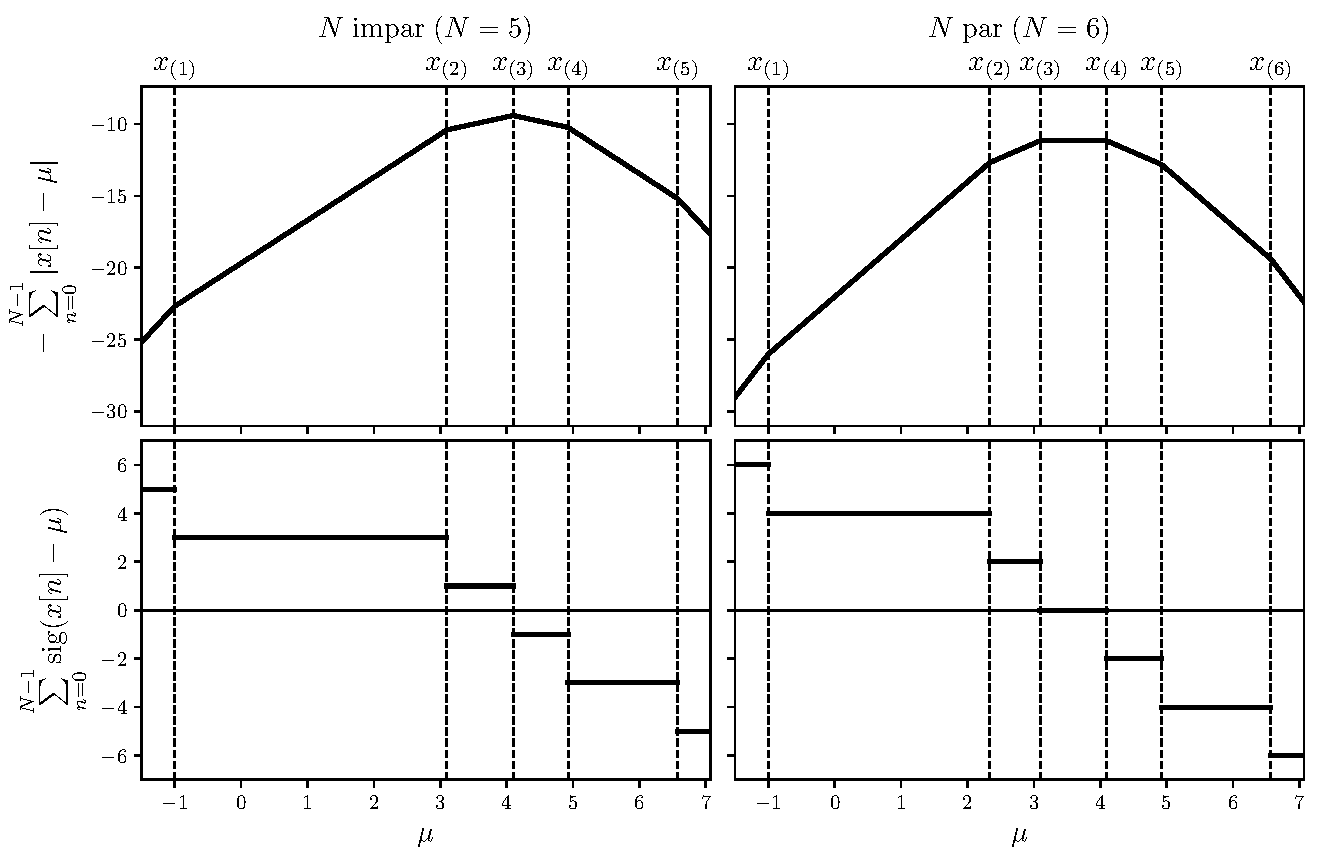
\includegraphics[width=1\textwidth]{figuras/example_mle_mean_laplace.pdf}
\caption{\label{fig:example_mle_mean_laplace} Función de verosimilitud logarítmica y su derivada cuando las observaciones son muestras IID con PDF de Laplace con \(\mu=4\) y \(\sigma=1\). Las líneas punteadas verticales indican los valores de las observaciones. Se observa que la verosimilitud es una función continua. En el caso en que \(N\) es impar, la verosimilitud es máxima en \(x_{(N+1)/2}\), si bien la derivada no existe en ese valor. Si \(N\) es par, la verosimilitud es máxima en el segmento horizontal \([x_{(N/2)},\,x_{(N/2+1)}]\). En ambos casos, la verosimilitud se maximiza en \(\mu=\operatorname{mediana}(\x)\).}
\end{center}
\end{figure}
Además, la gráfica de \(\ln p(\x;\,\mu)\) es una función continua lineal a trozos, como se muestra en la figura. Se observa que si \(N\) es impar, \(\ln p(\x;\,\mu)\) es estrictamente creciente en el intervalo \((-\infty,\,x_{(N+1)/2}]\) y estrictamente decreciente en el intervalo \([x_{(N+1)/2},\,\infty)\) y por lo tanto, la verosimilitud se maximiza en \(\mu=x_{(N+1)/2}\). Observar que si bien la función tiene un máximo absoluto, la derivada nunca se anula. Concretamente, la derivada no existe en el punto donde se da el máximo. En el caso en que \(N\) es par, el máximo de la función se da en el segmento horizontal \([x_{(N/2)},\,x_{(N/2+1)}]\), como se aprecia en la figura \ref{fig:example_mle_mean_laplace}. Teniendo en cuenta que la mediana se define como \(x_{(N+1)/2}\) si \(N\) es impar y \((x_{(N/2)}+x_{(N/2+1)})/2\), es decir, el punto medio del segmento \([x_{(N/2)},\,x_{(N/2+1)}]\) si \(N\) es par, se concluye que el MLE es
\[
 \hat{\mu}=\operatorname{mediana}(\x).
\]

\subsection{Ejemplo: MLE de la fase de una sinusoide}\label{sec:mle_sinusoidal_phase}

Se reconsidera el problema de la sección \ref{sec:crlb_sinusoidal_phase} de la estimación de la fase \(\phi\) de una sinusoide en WGN, o
\[
 x[n]=A\cos(2\pi f_0 n+\phi)+w[n],\qquad n=0,\,\dots,\,N-1,
\]
donde \(w[n]\) es WGN de varianza \(\sigma^2\) y la amplitud \(A\) y la frecuencia \(f_0\) de la sinusoide son conocidas. El MLE se obtiene maximizando la PDF respecto al parámetro. La PDF es
\[
 p(\x,\,\phi)=\frac{1}{(2\pi\sigma^2)^\frac{N}{2}}\exp\left\{-\frac{1}{2\sigma^2}\sum_{n=0}^{N-1}[x[n]-A\cos(2\pi f_0n+\phi)]^2\right\},
\]
y su maximización es equivalente a la minimización de la función
\[
 J(\phi)=\sum_{n=0}^{N-1}[x[n]-A\cos(2\pi f_0n+\phi)]^2.
\]
Diferenciando respecto a \(\phi\) se obtiene que
\[
 \frac{\partial J(\phi)}{\partial\phi}=2\sum_{n=0}^{N-1}[x[n]-A\cos(2\pi f_0n+\phi)]A\sin(2\pi f_0n+\phi),
\]
e igualando a cero, se obtiene que el MLE cumple que
\[
 \sum_{n=0}^{N-1}x[n]\sin(2\pi f_0n+\hat{\phi})=A\sum_{n=0}^{N-1}\cos(2\pi f_0n+\hat{\phi})\sin(2\pi f_0n+\hat{\phi}).
\]
Empleando la identidad trigonométrica \(\sin(2\theta)=2\sin\theta\cos\theta \) y la aproximación demostrada en el problema \ref{sec:problem_3_7}, el lado derecho de la igualdad puede ser aproximado como
\[
 \frac{1}{N}\sum_{n=0}^{N-1}\cos(2\pi f_0n+\hat{\phi})\sin(2\pi f_0n+\hat{\phi})
 =\frac{1}{2N}\sum_{n=0}^{N-1}\sin(4\pi f_0n+2\hat{\phi})\approx0
\]
si \(f_0\) no es cercano a 0 o a 1/2. Por lo tanto, al dividir el lado derecho entre \(N\) e igualar a cero, se obtiene que el MLE aproximado cumple que
\[
 \sum_{n=0}^{N-1}x[n]\sin(2\pi f_0n+\hat{\phi})=0
\]
Considerando que \(\sin(\alpha \pm \beta)=\sin\alpha\cos\beta\pm\cos\alpha\sin\beta\), se obtiene que
\[
 \sum_{n=0}^{N-1}x[n]\sin2\pi f_0n\cos\hat{\phi}=-\sum_{n=0}^{N-1}x[n]\cos2\pi f_0n\sin\hat{\phi},
\]
y finalmente, el MLE de la fase es aproximadamente
\[
 \hat{\phi}=-\arctan\frac{\displaystyle\sum_{n=0}^{N-1}x[n]\sin2\pi f_0n}{\displaystyle\sum_{n=0}^{N-1}x[n]\cos2\pi f_0n}.
\]
En el ejemplo de la sección \ref{sec:general_mvu_sinusoidal_phase_statistic} se encontró que no existe un estadístico suficiente individual en este problema. Los estadísticos suficientes están dados en la ecuación \ref{eq:general_mvu_sinusoidal_phase_statistics}. Se observa que el estimador MLE es una función de los estadísticos suficientes. Como la factorización de Neyman-Fisher resultó en
\[
 p(\x;\,\phi)=g(T_1(\x),\,T_2(\x),\,\phi)h(\x),
\]
maximizar \(p(\x;\,\phi)\) respecto a \(\phi\) es equivalente a maximizar \(g\), ya que \(h(\x)\) siempre puede elegirse de forma que \(h(\x)>0\), y por lo tanto, \(\hat{\phi}\) debe ser una función de \(T_1(\x)\) y \(T_2(\x)\).

Las propiedades asintóticas del MLE pueden alcanzarse para un largo de datos \(N\) pequeño si la SNR es suficientemente grande. En efecto, sustituyendo el modelo de los datos en el MLE de la fase, el estimador puede escribirse como
\[
 \hat{\phi}=-\arctan\frac{\displaystyle\sum_{n=0}^{N-1}[A\cos(2\pi f_0 n+\phi)+w[n]]\sin2\pi f_0n}{\displaystyle\sum_{n=0}^{N-1}[A\cos(2\pi f_0 n+\phi)+w[n]]\cos2\pi f_0n}.
\]
Considerando las identidades trigonométricas \(2\cos\theta\sin\varphi=\sin(\theta+\varphi)-\sin(\theta-\varphi)\) y \(2\cos\theta\cos\varphi=\cos(\theta-\varphi)+\cos(\theta+\varphi)\), se tiene que
\[
 \def\arraystretch{2}
 \begin{array}{ccc}
  \cos(2\pi f_0n+\phi)\sin2\pi f_0n&=&\dfrac{1}{2}[\sin(4\pi f_0n+\phi)-\sin\phi]\\
  \cos(2\pi f_0n+\phi)\cos2\pi f_0n&=&\dfrac{1}{2}[\cos\phi+\cos(4\pi f_0n+\phi)],
 \end{array}
\]
y por lo tanto
\begin{align*}
 \hat{\phi}&=-\arctan\frac{\displaystyle\frac{A}{2}\sum_{n=0}^{N-1}[\sin(4\pi f_0n+\phi)-\sin\phi]+\sum_{n=0}^{N-1}w[n]\sin2\pi f_0n}{\displaystyle\frac{A}{2}\sum_{n=0}^{N-1}[\cos\phi+\cos(4\pi f_0n+\phi)]+\sum_{n=0}^{N-1}w[n]\cos2\pi f_0n}\\
  &=-\arctan\frac{\displaystyle-\frac{NA}{2}\sin\phi+\frac{A}{2}\sum_{n=0}^{N-1}\sin(4\pi f_0n+\phi)+\sum_{n=0}^{N-1}w[n]\sin2\pi f_0n}{\displaystyle\frac{NA}{2}\cos\phi+\frac{A}{2}\sum_{n=0}^{N-1}\cos(4\pi f_0n+\phi)+\sum_{n=0}^{N-1}w[n]\cos2\pi f_0n}\\
  &=\arctan\frac{\displaystyle\sin\phi-\frac{1}{N}\sum_{n=0}^{N-1}\sin(4\pi f_0n+\phi)-\frac{2}{NA}\sum_{n=0}^{N-1}w[n]\sin2\pi f_0n}{\displaystyle\cos\phi+\frac{1}{N}\sum_{n=0}^{N-1}\cos(4\pi f_0n+\phi)+\frac{2}{NA}\sum_{n=0}^{N-1}w[n]\cos2\pi f_0n}
\end{align*}
y finalmente, considerando nuevamente la aproximación demostrada en el problema \ref{sec:problem_3_7}, se obtiene que
\begin{equation}\label{eq:mle_sinusoidal_parameters_phi_estimator_alt}
 \hat{\phi}\approx\arctan\frac{\displaystyle\sin\phi-\frac{2}{NA}\sum_{n=0}^{N-1}w[n]\cos2\pi f_0n}{\displaystyle\cos\phi+\frac{2}{NA}\sum_{n=0}^{N-1}w[n]\sin2\pi f_0n}.
\end{equation}
Si la cantidad de datos \(N\) es grande y/o si la potencia de la sinusoide (\(A^2/2\)) es grande, los términos de ruido son pequeños. La condición de que el error de estimación sea pequeño es lo que le permite al MLE alcanzar la distribución asintótica. Ver el problema de la sección \ref{sec:problem_7_15} por una discusión adicional sobre esto.

\subsection{Ejemplo: nivel de DC en ruido no independiente no gaussiano}\label{sec:mle_dc_level_correlated_non_gaussian}

Se consideran las observaciones
\[
 x[n]=A+w[n]\qquad n=0,\,\dots,\,N-1
\]
donde cada muestra de \(w[n]\) tiene PDF \(p(w[n])\) simétrica respecto a \(w[n]=0\) y con valor máximo en \(w[n]=0\) como se muestra en el figura \ref{fig:example_7_7}.
\begin{figure}[!htb]
\begin{center}
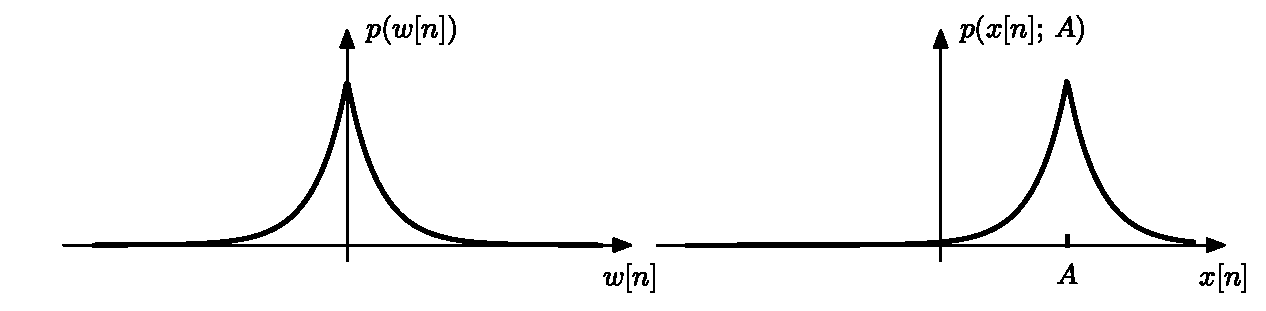
\includegraphics[width=0.9\textwidth]{figuras/example_7_7.pdf}
\caption{\label{fig:example_7_7} PDF no gaussiana del ruido \(w[n]\) y de las observaciones \(x[n]=A+w[n]\).}
\end{center}
\end{figure}
Además, se asume que todas las muestras de ruido son iguales, o \(w[0]=w[1]=\dots=w[N-1]\). Como todas las observaciones son idénticas, alcanza con considerar un única observación en la estimación de \(A\). Empleando solo \(x[0]\), se observa que la PDF de \(x[0]\) es una versión desplazada de \(p(w[n])\) una cantidad \(A\), como se muestra en la figura \ref{fig:example_7_7}. Esto es porque \(p_{x[0]}(x[0];\,A)=p_{w[0]}(x[0]-A)\) (ver el problema \ref{sec:problem_1_3}). El MLE de \(A\) es el valor que maximiza \(p_{w[0]}(x[0]-A)\), y es
\[
 \hat{A}=x[0].
\]
Este estimador tiene media
\[
 E(\hat{A})=E(x[0])=A
\]
ya que la PDF del ruido es simétrica respecto a \(w[0]=0\). La varianza de \(\hat{A}\) es la misma que la varianza de \(x[0]\) o \(w[0]\). Por lo tanto,
\[
 \var(\hat{A})=\int_{-\infty}^{\infty}u^2p_{w[0]}(u)\,du,
\]
mientras que la CRLB, como se dedujo en el problema \ref{sec:problem_3_2}, es
\[
 \var(\hat{A})\geq\left[\int_{-\infty}^{\infty}\frac{\left(\dfrac{dp_{w[0]}(u)}{du}\right)^2}{p_{w[0]}(u)}\,du\right]^{-1},
\]
y en general los dos valores son distintos (ver por ejemplo el problema de la sección \ref{sec:problem_7_16}). En este ejemplo, el error de estimación no decrece con el incremento del largo de los datos, sino que permanece constante. Además, la PDF de \(\hat{A}=x[0]\), es claramente es no gaussiana por ser la PDF de \(w[0]\) desplazada. Finalmente, el estimador \(\hat{A}\) ni siquiera es consistente.

\section{Algoritmo esperanza-maximización}

\subsection{Introducción}\label{sec:mle_em_introduction}

Un método para determinar de forma numérica el estimador MLE es el algoritmo esperanza-maximización (\emph{expectation-maximization}, EM). Es un algoritmo iterativo en el que en cada paso se obtiene una estimación del parámetro que incrementa la función de verosimilitud. Bajo  ciertas condiciones no muy exigentes, el algoritmo converge al menos a un máximo local. En esta sección se describe brevemente el algoritmo. Para hacerlo, se comienza considerando el ejemplo de estimación de las frecuencias de una mezcla de sinusoides, donde el modelo de los datos es
\[
 x[n]=\sum_{p=1}^{p}\cos2\pi f_in+w[n],\qquad n=0,\,\dots,\,N-1,
\]
donde \(w[n]\) es WGN de varianza \(\sigma^2\) y las frecuencias \(\mathbf{f}=[f_1\,\dots\,f_p]\) son los parámetros desconocidos a estimar. Como la PDF de los datos es
\[
 p(\x,\,\mathbf{f})=\frac{1}{(2\pi\sigma^2)^\frac{N}{2}}\exp\left[-\frac{1}{2\sigma^2}\sum_{n=0}^{N-1}\left(x[n]-\sum_{p=1}^{p}\cos2\pi f_in\right)^2\right],
\]
el algoritmo MLE  requiere la minimización de la función de dimensión \(p\)
\[
 J(\mathbf{f})=\left(x[n]-\sum_{p=1}^{p}\cos2\pi f_in\right)^2.
\]
Supóngase que el conjunto original de datos pudiera ser remplazado por el conjunto de datos independientes
\begin{equation}\label{eq:mle_em_frequency_decomposition}
 y_i[n]=\cos2\pi f_in+w_i[n],\qquad
 \begin{array}{rcl}
  i&=&1,\,\dots,\,p\\
  n&=&0,\,\dots,\,N-1
 \end{array}
\end{equation}
donde \(w_i[n]\) es WGN con varianza \(\sigma_i^2\). Asumiendo que los ruidos \(w_i[n]\) son procesos independientes, la PDF de los datos es
\begin{align}\label{eq:mle_em_frequency_pdf}
 p(\y;\,\mathbf{f})&=\prod_{i=1}^{p}p(\mathbf{y}_i;\,\mathbf{f})\nonumber\\
  &=\prod_{i=1}^{p}\frac{1}{(2\pi\sigma_i^2)^\frac{N}{2}}\exp\left[-\frac{1}{2\sigma_i^2}\sum_{n=0}^{N-1}\left(y_i[n]-\cos2\pi f_in\right)^2\right]\nonumber\\
  &=\left[\prod_{i=1}^{p}\frac{1}{(2\pi\sigma_i^2)^\frac{N}{2}}\right]\exp\left[-\sum_{i=1}^{p}\frac{1}{2\sigma_i^2}\sum_{n=0}^{N-1}\left(y_i[n]-\cos2\pi f_in\right)^2\right],
\end{align}
por lo que el problema quedó desacoplado y para maximizar la función de verosimilitud hay que minimizar
\[
 J(f_i)=\sum_{n=0}^{N-1}\left(y_i[n]-\cos2\pi f_in\right)^2,\qquad i=1,\,\dots,\,p.
\]
El problema original de la minimización de una función de dimensión \(p\) se redujo a la minimización separada de \(p\) funciones de una dimensión. El nuevo conjunto de datos \(\{y_1[n],\,\dots,\,y_p[n]\}\) se denomina \emph{datos completos} y se relaciona con el conjunto de datos original como
\begin{equation}\label{eq:mle_em_frequency_decomposition_x}
 x[n]=\sum_{i=1}^{p}y_i[n]
\end{equation}
si el ruido se descompone como
\[
 w[n]=\sum_{i=1}^{p}w_i[n],
\]
para lo cual se asume que los procesos de ruido \(w_i[n]\) son independientes y
\[
 \sigma^2=\sum_{i=1}^{p}\sigma^2_i[n].
\]
El problema es como obtener los datos completos a partir de los datos originales, o los datos \emph{incompletos}, teniendo que la descomposición no es única.

\subsection{El algoritmo EM}

Supóngase que se tiene la transformación de los datos incompletos a los datos completos
\[
 \x=\g(\y_1,\dots,\,\y_M)=\g(\y)
\]
donde en el ejemplo indicado antes \(M=p\) y los elementos de \(\y_i\) están dados por la ecuación \ref{eq:mle_em_frequency_decomposition}. 
El objetivo es encontrar el MLE de \(\thetabf\) mediante la maximización de \(p_x(\x;\,\thetabf)\). Debido a que este problema es difícil por tratarse de la maximización de una función de muchas variables, en su lugar se maximiza \(\ln p_y(\y;\,\thetabf)\). Como no se dispone de \(\y\), se reemplaza la función de verosimilitud logarítmica por su esperanza condicional
\[
 E_{y|x}[\ln p_y(\y;\,\thetabf)]=\int \ln p_y(\y;\,\thetabf)p(\y|\x;\,\thetabf)\,d\y.
\]
Finalmente, como se necesita conocer \(\thetabf\) para determinar \(p(\y|\x;\,\thetabf)\) y poder establecer la esperanza condicional, se emplea la estimación actual. Si \(\thetabf_k\) es la estimación \(k\)-ésima del MLE de \(\thetabf\), se emplea el siguiente algoritmo iterativo:

\paragraph{Esperanza (E):} Determinar la función de verosimilitud logarítmica promedio de los datos completos
\begin{equation}\label{eq:mle_em_algorithm_e_step}
 U(\thetabf,\,\thetabf_k)=\int \ln p_y(\y;\,\thetabf)p(\y|\x;\,\thetabf)\,d\y 
\end{equation}

\paragraph{Maximización (M):} Maximizar la función de verosimilitud logarítmica promedio de los datos completos
\begin{equation}\label{eq:mle_em_algorithm_m_step}
 \thetabf_{k+1}=\argmax_{\theta} U(\thetabf,\,\thetabf_k).
\end{equation}
En la convergencia, podría obtenerse el estimador MLE. Este enfoque se denomina \emph{algoritmo EM}. A continuación, se deduce el algoritmo para el problema de la estimación de las frecuencias de una mezcla de sinusoides empleado en la introducción.

\subsection{Ejemplo: estimación de las frecuencias de mezcla de sinusoides}

Continuando con el ejemplo de la sección \ref{sec:mle_em_introduction}, el objetivo es la deducción de la esperanza condicional de la función de verosimilitud logarítmica para aplicar el algoritmo EM. Se dedujo que la PDF de los datos completos está dada por la ecuación \ref{eq:mle_em_frequency_pdf}. Tomando el logaritmo  se obtiene la función de verosimilitud logarítmica,
\begin{align*}
 \ln p_y(\y;\,\theta)&=\ln\left[\prod_{i=1}^{p}\frac{1}{(2\pi\sigma_i^2)^\frac{N}{2}}\right]-\sum_{i=1}^{p}\frac{1}{2\sigma_i^2}\sum_{n=0}^{N-1}\left(y_i[n]-\cos2\pi f_in\right)^2\\
  &=-\frac{N}{2}\sum_{i=1}^p\ln2\pi\sigma_i^2-\sum_{i=1}^{p}\frac{1}{2\sigma_i^2}\sum_{n=0}^{N-1}\left(y^2_i[n]-2y_i[n]\cos2\pi f_in+\cos^22\pi f_in\right)\\
  &=-\frac{N}{2}\sum_{i=1}^p\ln2\pi\sigma_i^2-\sum_{i=1}^{p}\frac{1}{2\sigma_i^2}\sum_{n=0}^{N-1}y^2_i[n]+\sum_{i=1}^{p}\frac{1}{\sigma_i^2}\sum_{n=0}^{N-1}\left(y_i[n]\cos2\pi f_in-\frac{1}{2}\cos^22\pi f_in\right).
\end{align*}
Considerando la aproximación
\[
 \sum_{n=0}^{N-1}\cos^22\pi f_in=\sum_{n=0}^{N-1}\left(\frac{1}{2}+\frac{1}{2}\cos4\pi f_in\right)\approx\frac{N}{2},
\]
donde se usó la ecuación \ref{eq:sum_n_raised_i_cos_alpha_n} demostrada en el apéndice \ref{ap:sum_n_raised_i_cos_alpha_n}, se obtiene que
\begin{align*}
 \ln p_y(\y;\,\theta)&=-\frac{N}{2}\sum_{i=1}^p\ln2\pi\sigma_i^2-\sum_{i=1}^{p}\frac{1}{2\sigma_i^2}\sum_{n=0}^{N-1}y^2_i[n]-\frac{N}{4}\sum_{i=1}^{p}\frac{1}{\sigma_i^2}+\sum_{i=1}^{p}\frac{1}{\sigma_i^2}\sum_{n=0}^{N-1}y_i[n]\cos2\pi f_in\\
  &=h(\y)+\sum_{i=1}^{p}\frac{1}{\sigma_i^2}\sum_{n=0}^{N-1}y_i[n]\cos2\pi f_in,
\end{align*}
donde \(h(\y)\) es la suma de los tres primeros sumandos y como no depende del parámetro, no afecta en la maximización de la función. Definiendo \(\mathbf{c}_i=[1\,\cos2\pi f_i\dots\cos2\pi f_i(N-1)]^T\), se llega a que
\[
 \ln p_y(\y;\,\theta)=h(\y)+\sum_{i=1}^p\frac{1}{\sigma_i^2}\mathbf{c}^T_i\y_i.
\]
Concatenando los \(\mathbf{c}_i\) y los \(\y_i\) como
\[
 \mathbf{c}=
 \begin{bmatrix}
  \dfrac{1}{\sigma_1^2}\mathbf{c}_1\\
  \vdots\\
  \dfrac{1}{\sigma_p^2}\mathbf{c}_p
 \end{bmatrix}\qquad\qquad
 \mathbf{\y}=
 \begin{bmatrix}
  \y_1\\
  \vdots\\
  \y_p
 \end{bmatrix}
\]
se tiene que
\[
 \ln p_y(\y;\,\theta)=h(\y)+\mathbf{c}^T\y.
\]
Notar que los vectores \(\mathbf{c}\) y \(\y\) tienen dimensiones \(Np\times1\). De la ecuación \ref{eq:mle_em_algorithm_e_step} del paso E, la esperanza condicional es
\begin{align}\label{eq:mle_em_frequency_e_step}
 U(\thetabf,\,\thetabf_k)&=E[\ln p_y(\y;\,\theta)|\x;\,\thetabf_k]\nonumber\\
   &=E[h(\y)|\x;\,\thetabf_k]+\mathbf{c}^TE[\y|\x;\,\thetabf_k].
\end{align}
Como se quiere maximizar \(U(\thetabf,\,\thetabf_k)\) con respecto a \(\thetabf\), se puede omitir el valor esperado de \(h(\y)\) ya que no depende de \(\thetabf\). Ahora, los vectores \(\y\) y \(\x\) son conjuntamente gaussiansos, ya que, del la ecuación \ref{eq:mle_em_frequency_decomposition_x}
\[
 \x=\sum_{i=1}^p\y_i=[\I\,\I\dots\I]\y,
\]
donde \(\I\) es la matriz identidad \(N\times N\) y la matriz de transformación está compuesta de \(p\) matrices identidad, por lo que tiene dimensiones \(N\times Np\). Empleando el resultado de la esperanza condicional de vectores conjuntamente gaussianos deducido en el apéndice \ref{ap:conditional_pdf_joint_gaussian} dado por la ecuación \ref{eq:conditional_joint_multivariate_gaussian_mean}, se tiene que
\[
 E(\y|\x;\,\thetabf_k)=E(\y)+\C_{yx}\C_{xx}^{-1}(\x-E(\x)).
\]
Teniendo en cuenta que \(\y_i=\mathbf{c}_i+\w_i\), las medias son
\[
 E(\y)=
 \begin{bmatrix}
  \mathbf{c}_1\\
  \vdots\\
  \mathbf{c}_p
 \end{bmatrix}\qquad\qquad
 E(\x)=\sum_{i=1}^p\mathbf{c}_i
\]
y las matrices de covarianza son
\[
 \C_{xx}=\sigma^2\I
\]
de dimensiones \(N\times N\) y
\begin{align*}
 C_{yx}&=E\left(
  \begin{bmatrix}
   \w_1\\
   \w_2\\
   \vdots\\
   \w_p
  \end{bmatrix}\w^T\right)\\
  &=E\left(
  \begin{bmatrix}
   \w_1\\
   \w_2\\
   \vdots\\
   \w_p
  \end{bmatrix}
  \left\{
  \begin{bmatrix}
   \I&\I&\dots&\I
  \end{bmatrix}
  \begin{bmatrix}
   \w_1\\
   \w_2\\
   \vdots\\
   \w_p
  \end{bmatrix}
  \right\}^T\right)\\
  &=
  \begin{bmatrix}
   \sigma_1^2\I & \mathbf{0} & \dots & \mathbf{0}\\
   \mathbf{0} & \sigma_2^2\I & \dots & \mathbf{0}\\
   \vdots & \vdots & \ddots & \vdots\\
   \mathbf{0} & \mathbf{0} & \dots  & \sigma_p^2\I\\
  \end{bmatrix}
  \begin{bmatrix}
   \I\\
   \I\\
   \vdots\\
   \I
  \end{bmatrix}\\
  &=
  \begin{bmatrix}
   \sigma_1^2\I\\
   \sigma_2^2\I\\
   \vdots\\
   \sigma_p^2\I\\
  \end{bmatrix}
\end{align*}
Sustituyendo estos resultados en la esperanza condicional, se tiene que
\begin{align*}
 E(\y|\x;\,\thetabf_k)&=
 \begin{bmatrix}
  \mathbf{c}_1\\
  \vdots\\
  \mathbf{c}_p
 \end{bmatrix}+
 \begin{bmatrix}
   \sigma_1^2\I\\
   \vdots\\
   \sigma_p^2\I
  \end{bmatrix}
  \frac{1}{\sigma^2}\I
  \left(\x-\sum_{i=1}^p\mathbf{c}_i\right)\\
  &=
  \begin{bmatrix}
  \mathbf{c}_1\\
  \vdots\\
  \mathbf{c}_p
 \end{bmatrix}+
 \begin{bmatrix}
   \displaystyle\frac{\sigma_1^2}{\sigma^2}\left(\x-\sum_{i=1}^p\mathbf{c}_i\right)\\
   \vdots\\
   \displaystyle\frac{\sigma_p^2}{\sigma^2}\left(\x-\sum_{i=1}^p\mathbf{c}_i\right)
  \end{bmatrix},
\end{align*}
donde se observa que el problema quedó desacoplado en \(p\) problemas separados,
\[
 E(\y_i|\x;\,\thetabf_k)=\mathbf{c}_i+\frac{\sigma_i^2}{\sigma^2}\left(\x-\sum_{i=1}^p\mathbf{c}_i\right),\qquad i=1,\,\dots,\,p
\]
donde \(\mathbf{c}_i\) se calcular empleando \(\thetabf_k\). Notar que \(E(\y_i|\x;\,\thetabf_k)\) puede ser pensado como un estimador de los datos \(y_i[n]\), ya que, llamando \(\hat{\y}_i=E(\y_i|\x;\,\thetabf_k)\),
\[
 \hat{y}_i[n]=\cos2\pi f_{i_k}n+\frac{\sigma_i^2}{\sigma^2}\left(x[n]-\sum_{i=1}^p\cos2\pi f_{i_k}n\right)
\]
donde el término entre paréntesis es un estimador de \(w[n]\) y por lo tanto, el segundo sumando es un estimador de \(w_i[n]\)  en el paso \(k\)-ésimo.
Descartando el término independiente de \(\thetabf\) en la ecuación \ref{eq:mle_em_frequency_e_step}, se quiere maximizar sobre \(\thetabf\)
\[
 U'(\thetabf,\,\thetabf_k)=\mathbf{c}^T\y=\sum_{i=1}^{p}\mathbf{c_i}^T\hat{\y}_i,
\]
lo cual se hace maximizando cada termino de la suma separadamente,
\[
 f_{i_{k+1}}=\argmax_{f_i}\mathbf{c}_i\hat{\y}_i.
\]
Por último, como los \(\sigma^2_i\) no son únicos, pueden elegirse arbitrariamente siempre que se cumpla que
\[
 \sum_{i=1}^p\sigma^2_i=\sigma^2,
\]
o equivalentemente
\[
 \sum_{i=1}^p\beta_i=\sum_{i=1}^p\frac{\sigma_i^2}{\sigma^2}=1.
\]
Resumiendo, el algoritmo EM para la estimación de las frecuencias es
\paragraph{Paso E:} Para \(i=1,\,\dots,\,p\)
\[
 \hat{y}_i[n]=\cos2\pi f_{i_k}n+\beta_i\left(x[n]-\sum_{i=1}^p\cos2\pi f_{i_k}n\right).
\]
\paragraph{Paso M:} Para \(i=1,\,\dots,\,p\)
\[
 f_{i_{k+1}}=\argmax_{f_i}\sum_{n=0}^{N-1}\hat{y}_i[n]\cos2\pi f_in,
\]
donde los \(\beta_i\) pueden ser elegidos de forma arbitraria siempre que \(\sum_{i=1}^p\beta_i=1\).

El algoritmo desacopla iterativamente los datos originales en \(p\) conjunto de datos separados, donde cada uno consiste en una única sinusoide en WGN. La maximización obtenida corresponde al MLE de una única sinusoide en ruido con el conjunto de datos dado por los datos completos estimados, como se muestra en el problema de la sección \ref{sec:problem_7_19}. Mas detalles pueden encontrarse en \cite{feder1988parameter}.

\section{MLE asintótico}\label{sec:mle_asymptotic_gaussian}

En ocasiones es difícil evaluar el MLE de un parámetro con PDF gaussiana debido a la necesidad de invertir una matriz de covarianza de dimensiones grandes. Por ejemplo, si \(\x\sim\mathcal{N}(\mathbf{0},\,\C(\thetabf))\), el MLE se obtiene maximizando
\[
 p(\x,\,\thetabf)=\frac{1}{(2\pi)^\frac{N}{2}\det^\frac{N}{2}(\C)}\exp\left[-\frac{1}{2}\x^T\C^{-1}\x\right].
\]
Si no es posible obtener una fórmula cerrada de la matriz inversa, la busqueda del estimador requiere la inversión numérica de una matriz \(N\times N\) en cada iteración. En el caso en que los datos \(\x\) son un proceso WSS de media nula de forma que la matriz de covarianza es Toeplitz, puede emplearse un método alternativo aproximado. Como se mostró en la sección \ref{sec:crlb_general_gaussian_wss}, la función de verosimilitud logarítmica asintótica, es decir, cuando la cantidad de datos es grande, es (ecuación \ref{eq:crlb_asymptotic_gaussian_likelihood_2})
\begin{equation}\label{eq:mle_asymptotic_gaussian_likelihood}
  \ln p(\x;\,\thetabf)=-\frac{N}{2}\ln 2\pi -\frac{N}{2}\int_{-\frac{1}{2}}^{\frac{1}{2}}\left[\ln P_{xx}(f)+\frac{I(f)}{P_{xx}(f)}\right]\,df.
\end{equation}
donde
\[
 I(f)=\frac{1}{N}\left|\sum_{n=0}^{N-1}x[n]e^{-j2\pi fn}\right|^2
\]
es el periodograma de los datos y \(P_{xx}(f)\) es la PSD. La dependencia de la función de verosimilitud logarítmica con el parámetro \(\thetabf\) es a través de la PSD. Diferenciando \ref{eq:mle_asymptotic_gaussian_likelihood} se obtiene que ((ecuación \ref{eq:crlb_asymptotic_gaussian_likelihood_first_derivative}))
\[
 \frac{\partial\ln p(\x;\,\thetabf)}{\partial\theta_i}=-\frac{N}{2}\int_{-\frac{1}{2}}^{\frac{1}{2}}\left[\frac{1}{P_{xx}(f)}-\frac{I(f)}{P_{xx}^2(f)}\right]\frac{\partial P_{xx}(f)}{\partial\theta_i}\,df,
\]
por lo que las condiciones necesarias del MLE son
\begin{equation}\label{eq:mle_asymptotic_gaussian_mle_condition} 
 \int_{-\frac{1}{2}}^{\frac{1}{2}}\left[\frac{1}{P_{xx}(f)}-\frac{I(f)}{P_{xx}^2(f)}\right]\frac{\partial P_{xx}(f)}{\partial\theta_i}\,df=0. 
\end{equation}
La derivada segunda está dada por la ecuación \ref{eq:crlb_asymptotic_gaussian_likelihood_derivatives} por lo que podría emplearse algún método iterativo como el de Newton-Raphson para encontrar el máximo.

\subsection{Ejemplo: proceso de media móvil gaussiano}

Un proceso WSS tiene ACF
\begin{equation}\label{eq:mle_asymptotic_ma2_autocorrelation}
  r_{xx}[k]=\left\{
 \begin{array}{ll}
  1+b^2[1]+b^2[2] & k=0\\
  b[1]+b[1]b[2] & k=1\\
  b[2] & k=2\\
  0 & k\geq 3.
 \end{array}
 \right.
\end{equation}
y se quiere calcular el MLE de los coeficientes \(b[1]\) y \(b[2]\). Para hacerlo, se comenzará mostrando que la PSD es
\[
 P_{xx}(f)=\left|1+b[1]e^{-j2\pi f}+b[2]e^{-j4\pi f}\right|^2.
\]
La transformada \(z\) de la ACF es
\begin{equation}\label{eq:mle_ma_example_psd_tmp}
 P_{xx}(z)=b[2]z^2+(b[1]+b[1]b[2])z+(1+b^2[1]+b^2[2])+(b[1]+b[1]b[2])z^{-1}+b[2]z^{-2}.
\end{equation}
Además, el proceso \(x[n]\) se obtiene filtrando WGN de varianza \(\sigma_{ww}^2=1\) mediante un filtro de función de transferencia \(\mathcal{B}(z)=a_0+a_1z^{-1}+a_2z^{-2}\), por lo que la PSD se puede expresar como (ver el capítulo 3 de \cite{hayes96statistical})
\begin{align*}
 P_{xx}(z)&=P_{ww}(z)\mathcal{B}(z)\mathcal{B}(1/z)\\
  &=(a_0+a_1z^{-1}+a_2z^{-2})(a_0+a_1z^{1}+a_2z^{2})\\
  &=a_0a_2z^2+(a_0a_1+a_1a_2)z+(a_0^2+a_1^2+a_2^2)+(a_0a_1+a_1a_2)z^{-1}+a_0a_2z^{-2}.
\end{align*}
Igualando esta ecuación con la ecuación \ref{eq:mle_ma_example_psd_tmp}, se obtiene que los coeficientes del filtro generador son 
\[
 a_0=1,\qquad\qquad a_1=b[1],\qquad\qquad a_2=b[2],
\]
resultando en 
\[
 \mathcal{B}(z)=1+b[1]z^{-1}+b[2]z^{-2}.
\]
Se concluye que la PSD de los datos es
\[
 P_{xx}(f)=P_{ww}(f)|\mathcal{B}(f)|^2=\left|1+b[1]e^{-j2\pi f}+b[2]e^{-j4\pi f}\right|^2,
\]
y se trata de un proceso MA de orden 2. Para calcular el MLE de los parámetros de filtro, es necesario invertir la matriz de covarianza. En su lugar, se puede maximizar la ecuación \ref{eq:mle_asymptotic_gaussian_likelihood}. Típicamente, se asume que el filtro \(\mathcal{B}(z)\) es de fase mínima, es decir, todos los ceros se encuentran dentro del círculo unidad. En ese caso, como se muestra en el problema de la sección \ref{sec:problem_7_22}, se cumple que
\[
 \int_{-\frac{1}{2}}^{\frac{1}{2}}\ln P_{xx}(f)\,df=0,
\]
por lo que maximizar la ecuación \ref{eq:mle_asymptotic_gaussian_likelihood} es equivalente a minimizar
\begin{equation*}
  \int_{-\frac{1}{2}}^\frac{1}{2}\frac{I(f)}{\left|1+b[1]e^{-j2\pi f}+b[2]e^{-j4\pi f}\right|^2}\,df.
\end{equation*}
Además, la función de transferencia se puede factorizar como
\[
 \mathcal{B}(z)=(1-z_1z^{-1})(1-z_2z^{-1})
\]
donde \(z_1\) y \(z_2\) son los ceros del sistema y cumplen que son reales o complejos conjugados con \(|z_1|<1\) y \(|z_2|<1\). Por lo tanto, el MLE se encuentra minimizando
\begin{equation}\label{eq:mle_asymptotic_ma2_log_likelihood}
 \int_{-\frac{1}{2}}^\frac{1}{2}\frac{I(f)}{\left|1-z_1e^{-j2\pi f}\right|^2\left|1-z_2e^{-j2\pi f}\right|^2}\,df 
\end{equation}
sobre los valores permitidos de \(z_1\) y \(z_2\), y luego, considerando que
\[
 (1-z_1e^{-j2\pi f})(1-z_2e^{-j2\pi f})=1-(z_1+z_2)e^{-j2\pi f}+z_1z_2e^{-j2\pi f},
\]
los coeficientes se obtienen como
\[
 b[1]=-(z_1+z_2),\qquad\qquad b[2]=z_1z_2.
\]
Para la minimización puede emplearse la búsqueda sobre una grilla en el plano complejo o algún método iterarivo. La restricción de que \(z_1\) y \(z_2\) son reales o complejos conjugados limita la búsqueda, y es necesaria para que los coeficientes del filtro generador, y por lo tanto el proceso \(x[n]\), sean reales.

Se realizó una simulación por computadora del cálculo del MLE asintótico de los parámetros \(b[1]\) y \(b[2]\) de un proceso MA(2), cuya ACF está dada por la ecuación \ref{eq:mle_asymptotic_ma2_autocorrelation}, mediante la búsqueda del mínimo de la ecuación \ref{eq:mle_asymptotic_ma2_log_likelihood}. Para esto se generaron \(N=150\) muestras del proceso MA(2) con parámetros \(b[1]=-0.9\) y \(b[2]=0.81\), que corresponde a un filtro generador \(\mathcal{B}(z)\) con ceros en \(z_{1,\,2}=0.9e^{\pm j\pi/6}\), se construyó una grilla en el semicírculo unidad del plano complejo y se evaluó la ecuación \ref{eq:mle_asymptotic_ma2_log_likelihood} en cada punto de la grilla. El estimador MLE de \(z_1\) es el valor de la grilla en donde la función toma el menor valor, y \(z_2=z_1^*\). El resultado se muestra en la figura \ref{fig:example_7_14}.
\begin{figure}[!htb]
\begin{center}
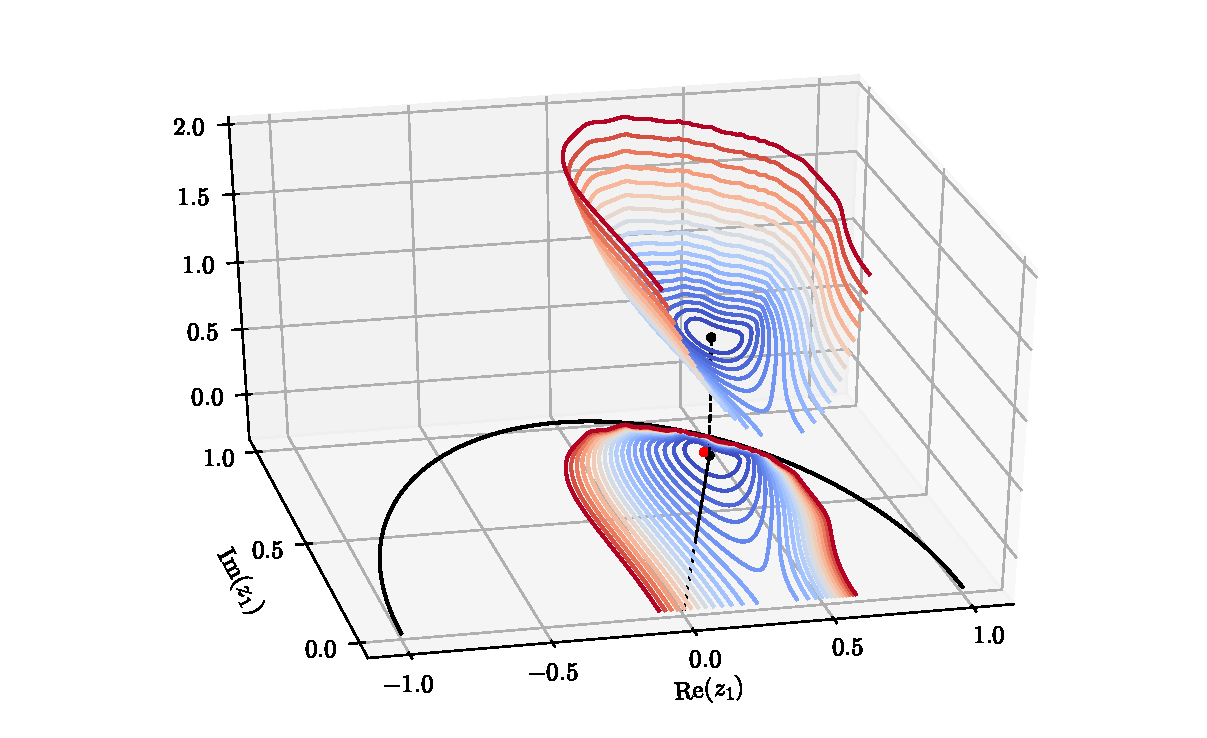
\includegraphics[width=1\textwidth]{figuras/example_7_14.pdf}
\caption{\label{fig:example_7_14} MLE asintótico de los parámetros de un proceso MA(2). Se muestra la superficie definida por la ecuación \ref{eq:mle_asymptotic_ma2_log_likelihood} en el plano complejo mediante curvas de nivel. El mínimo de la superficie corresponde al MLE del cero \(z_1\) del proceso MA(2), y se marca con un punto negro. El valor verdadero del parámetro está marcado con el punto en rojo.}
\end{center}
\end{figure}
Para la realización mostrada en la figura, el mínimo de la superficie está en \(\hat{z}_1\) de módulo \(|\hat{z}_1|\approx0.89\) y argumento \(\arg(\hat{z}_1)\approx1.03\) rad, lo que corresponde a los estimadores
\[
 \hat{b}[1]=-2|\hat{z}_1|\cos[\arg(\hat{z}_1)]\approx-0.92\qquad\qquad\textrm{y}\qquad\qquad\hat{b}[2]=|\hat{z}_1|^2\approx 0.79.
\]
El resultado mejora al incrementar la cantidad \(N\) de muestras del proceso. La ecuación \ref{eq:mle_asymptotic_ma2_log_likelihood} debe evaluarse para cada punto de la grilla y por lo tanto, puede ser computacionalmente costoso. Para hacerlo de forma eficiente, notar que \(I(f)\) solo depende de los datos \(x[n]\) y no de los valores \(z_1\) de la grilla, por lo que se calcula una sola vez mediante la transformada discreta de Fourier (\emph{discrete Fourier transform}, DFT) con relleno de ceros para obtener una cantidad de muestras apropiada en la frecuencia y lograr un cálculo preciso de la integral de forma numérica, empleando por ejemplo, la regla del trapecio. El denominador en la integral es distinto para cada complejo \(z_1\) en la grilla, y para calcularlo de forma eficiente, se aplica la DTF a la secuencia \([1,\, -2|z_1|\cos[\arg(z_1)],\,|z_1|^2]\) con el relleno de ceros apropiado para tener la misma cantidad de muestras en frecuencia que el numerador. Se tuvo en cuenta además que el integrando es simétrico, por lo que alcanza con integrar en el intervalo entre 0 y \(1/2\).

\section{Ejemplos de procesamiento de señales}

\subsection{Ejemplo: estimación de los parámetros de una sinusoide}\label{sec:mle_sinusoidal_parameters}

En la sección \ref{sec:sinusoidal_parameter_estimation} se calculó la CRLB de los parámetros de una sinusoide en WGN. Se determinará a continuación el MLE de la amplitud \(A\), la frecuencia \(f_0\) y la fase \(\phi\). Los datos observados son
\[
 x[n]=A\cos(2\pi f_0n+\phi)+w[n]\qquad  n=0,\,1,\dots,\,N-1,
\]
con \(A>0\) y \(0<f_0<1/2\). La PDF de los datos es
\[
 p(\x;\,\thetabf)=\frac{1}{(2\pi\sigma^2)^\frac{N}{2}}\exp\left[-\frac{1}{2\sigma^2}\sum_{n=0}^{N-1}(x[n]-A\cos(2\pi f_0n+\phi))^2\right],
\]
por lo que el MLE de la amplitud \(A\), la frecuencia \(f_0\) y la fase \(\phi\) se obtienen minimizando
\[
 J(A,\,f_0,\,\phi)=\sum_{n=0}^{N-1}(x[n]-A\cos(2\pi f_0n+\phi))^2.
\]
Considerando que \(\cos(\alpha\pm\beta )=\cos\alpha\cos\beta\mp\sin\alpha\sin\beta\) se tiene que
\[
 J(A,\,f_0,\,\phi)=\sum_{n=0}^{N-1}(x[n]-A\cos\phi\cos2\pi f_0n+A\sin\phi\cos2\pi f_0n)^2.
\]
Aunque \(J\) no es una forma cuadrática en \(A\) y \(\phi\), se puede transformar en una forma cuadrática definiendo
\[
 \alpha_1=A\cos\phi,\qquad\qquad\alpha_2=A\sin\phi,
\]
que se trata de una transformación uno a uno. La transformación inversa es
\begin{equation}\label{eq:mle_sinusoidal_parameters_transformation}
 A=\sqrt{\alpha_1^2+\alpha_2^2},\qquad\qquad\phi=\arctan\left(\frac{-\alpha_2}{\alpha_1}\right). 
\end{equation}
Sean
\[
 \mathbf{c}=[1\;\cos2\pi f_0\,\dots\,\cos2\pi f_0(N-1)]^T
 \qquad\qquad\textrm{y}\qquad\qquad
 \s=[0\;\sin2\pi f_0\,\dots\,\sin2\pi f_0(N-1)]^T.
\]
La función a minimizar queda
\begin{align*}
 J'(\alpha_1,\,\alpha_2,\,f_0)&=(\x-\alpha_1\mathbf{c}-\alpha_1\s)(\x-\alpha_1\mathbf{c}-\alpha_1\s)^T\\
  &=(\x-\Hbf\alphabf)^T(\x-\Hbf\alphabf),
\end{align*}
donde \(\alphabf=[\alpha_1\,\alpha_2]^T\) y \(\Hbf=[\mathbf{c}\,\s]\) es una matriz \(N\times2\).
Se observa que la función a minimizar sobre \(\alphabf\) es la misma que la encontrada en el modelo lineal dada por la ecuación \ref{eq:mle_linear_model_j} con \(\C=\I\). Por lo tanto, de la ecuación \ref{eq:mle_linear_model_estimator}, \(J'\) se minimiza con 
\begin{equation}\label{eq:mle_sinusoidal_parameters_alpha_estimator}
 \hat{\alphabf}=(\Hbf^T\Hbf)^{-1}\Hbf^T\x.
\end{equation}
Luego,
\begin{align*}
 J'(\hat{\alpha_1},\,\hat{\alpha_2},\,f_0)&=(\x-\Hbf\hat{\alphabf})^T(\x-\Hbf\hat{\alphabf})\\
   &=(\x-\Hbf(\Hbf^T\Hbf)^{-1}\Hbf^T\x)^T(\x-\Hbf(\Hbf^T\Hbf)^{-1}\Hbf^T\x)\\
   &=\x^T(\I-\Hbf(\Hbf^T\Hbf)^{-1}\Hbf^T)^T(\I-\Hbf(\Hbf^T\Hbf)^{-1}\Hbf^T)\x\\
   &\overset{(a)}{=}\x^T(\I-\Hbf(\Hbf^T\Hbf)^{-1}\Hbf^T)\x
\end{align*}
donde en \((a)\) se consideró que \(\I-\Hbf(\Hbf^T\Hbf)^{-1}\Hbf^T\) es una matriz idempotente (una matriz idempotente cumple que \(\A^2=\A\)), ya que
\begin{align*}
 (\I-\Hbf(\Hbf^T\Hbf)^{-1}\Hbf^T)^T(\I-\Hbf(\Hbf^T\Hbf)^{-1}\Hbf^T)&=
  (\I-\Hbf(\Hbf^T\Hbf)^{-1}\Hbf^T)(\I-\Hbf(\Hbf^T\Hbf)^{-1}\Hbf^T)\\
  &=\I-\Hbf(\Hbf^T\Hbf)^{-1}\Hbf^T-\Hbf(\Hbf^T\Hbf)^{-1}\Hbf^T\\
  &\quad+\Hbf(\Hbf^T\Hbf)^{-1}\Hbf^T\Hbf(\Hbf^T\Hbf)^{-1}\Hbf^T\\
  &=\I-\Hbf(\Hbf^T\Hbf)^{-1}\Hbf^T-\Hbf(\Hbf^T\Hbf)^{-1}\Hbf^T\\
  &\quad+\Hbf(\Hbf^T\Hbf)^{-1}\Hbf^T\\
  &=\I-\Hbf(\Hbf^T\Hbf)^{-1}\Hbf^T.
\end{align*}
De esta forma, para encontrar \(\hat{f}_0\) se necesita minimizar \(J'\) sobre \(f_0\) o equivalentemente, maximizar
\[
 \x^T\Hbf(\Hbf^T\Hbf)^{-1}\Hbf^T\x.
\]
Como \(\Hbf=[\mathbf{c}\,\s],\) se tiene que
\[
 \Hbf^T\x=
 \begin{bmatrix}
  \mathbf{c}^T\\
  \s^T
 \end{bmatrix}
 \x=
 \begin{bmatrix}
  \mathbf{c}^T\x\\
  \s^T\x
 \end{bmatrix},\qquad\qquad
 \Hbf^T\Hbf=
 \begin{bmatrix}
  \mathbf{c}^T\\
  \s^T
 \end{bmatrix}
 \begin{bmatrix}
  \mathbf{c} & \s
 \end{bmatrix}=
 \begin{bmatrix}
  \mathbf{c}^T\mathbf{c} & \mathbf{c}^T\s\\
  \s^T\mathbf{c} & \s^T\s
 \end{bmatrix}
\]
y la función a maximizar es
\begin{equation}\label{eq:mle_sinusoidal_parameters_maximization_f0}
  \begin{bmatrix}
  \mathbf{c}^T\x\\
  \s^T\x
 \end{bmatrix}^T
 \begin{bmatrix}
  \mathbf{c}^T\mathbf{c} & \mathbf{c}^T\s\\
  \s^T\mathbf{c} & \s^T\s
 \end{bmatrix}^{-1}
 \begin{bmatrix}
  \mathbf{c}^T\x\\
  \s^T\x
 \end{bmatrix}.
\end{equation}
Una vez que se encuentra \(\hat{f}_0\) empleando la expresión anterior, \(\hat{\alphabf}\) se encuentra empleando la ecuación \ref{eq:mle_sinusoidal_parameters_alpha_estimator} y luego, \(\hat{A}\) y \(\hat{\phi}\) mediante la ecuación \ref{eq:mle_sinusoidal_parameters_transformation}. Puede obtenerse una aproximación del MLE considerando que
\begin{align*}
 \mathbf{c}^T\mathbf{c}&=\sum_{n=0}^{N-1}\cos^22\pi f_0n=\sum_{n=0}^{N-1}\frac{1+\cos4\pi f_0n}{2}
  =\frac{N}{2}\left(1+\frac{1}{N}\sum_{n=0}^{N-1}\cos4\pi f_0n\right)\approx\frac{N}{2}\\
  \s^T\s&=\sum_{n=0}^{N-1}\sin^22\pi f_0n=\sum_{n=0}^{N-1}\frac{1-\cos4\pi f_0n}{2}
  =\frac{N}{2}\left(1-\frac{1}{N}\sum_{n=0}^{N-1}\cos4\pi f_0n\right)\approx\frac{N}{2}\\
 \mathbf{c}^T\s=\s^T\mathbf{c}&=\sum_{n=0}^{N-1}\sin2\pi f_0n\cos2\pi f_0n 
  =\frac{1}{2}\sum_{n=0}^{N-1}\sin4\pi f_0n,
\end{align*}
donde en las aproximaciones se empleó el resultado demostrado en el apéndice \ref{ap:sum_n_raised_i_cos_alpha_n}, que es válido si \(f_0\) no es cercano a 0 ni a 1/2. Por lo tanto,
\begin{align*}
 \begin{bmatrix}
  \mathbf{c}^T\mathbf{c} & \mathbf{c}^T\s\\
  \s^T\mathbf{c} & \s^T\s
 \end{bmatrix}^{-1}&\approx
 \begin{bmatrix}
  \displaystyle\frac{N}{2} & \displaystyle\frac{1}{2}\sum_{n=0}^{N-1}\sin4\pi f_0n\\
  \displaystyle\frac{1}{2}\sum_{n=0}^{N-1}\sin4\pi f_0n & \displaystyle\frac{N}{2}
 \end{bmatrix}^{-1}\\
 &=\frac{1}{\dfrac{N^2}{4}-\dfrac{1}{4}\left(\displaystyle\sum_{n=0}^{N-1}\sin4\pi f_0n\right)^2}
 \begin{bmatrix}
  \displaystyle\frac{N}{2} & \displaystyle-\frac{1}{2}\sum_{n=0}^{N-1}\sin4\pi f_0n\\
  \displaystyle-\frac{1}{2}\sum_{n=0}^{N-1}\sin4\pi f_0n & \displaystyle\frac{N}{2}
 \end{bmatrix}.
\end{align*}
Teniendo en cuenta que
\[
 \frac{N^2}{4}-\frac{1}{4}\left(\sum_{n=0}^{N-1}\sin4\pi f_0n\right)^2
 =\frac{N^2}{4}\left[1-\left(\frac{1}{N}\sum_{n=0}^{N-1}\sin4\pi f_0n\right)^2\right]
 \approx\frac{N^2}{4},
\]
se tiene que
\[
 \begin{bmatrix}
  \mathbf{c}^T\mathbf{c} & \mathbf{c}^T\s\\
  \s^T\mathbf{c} & \s^T\s
 \end{bmatrix}^{-1}=
 \begin{bmatrix}
  \displaystyle\frac{2}{N} & \displaystyle-\frac{2}{N^2}\sum_{n=0}^{N-1}\sin4\pi f_0n\\
  \displaystyle-\frac{2}{N^2}\sum_{n=0}^{N-1}\sin4\pi f_0n & \displaystyle\frac{2}{N}
 \end{bmatrix}\approx
 \begin{bmatrix}
  \displaystyle\frac{2}{N} & 0\\
  0 & \displaystyle\frac{2}{N}
 \end{bmatrix}=
 \frac{2}{N}\I.
\]
Con estas consideraciones, la ecuación \ref{eq:mle_sinusoidal_parameters_maximization_f0} a maximizar para encontrar \(\hat{f}_0\) queda
\begin{align*}
 \begin{bmatrix}
  \mathbf{c}^T\x &
  \s^T\x
 \end{bmatrix}
 \frac{2}{N}\I
 \begin{bmatrix}
  \mathbf{c}^T\x\\
  \s^T\x
 \end{bmatrix}
 &=\frac{2}{N}\left[(\mathbf{c}^T\x)^2+(\s^T\x)^2\right]\\
 &=\frac{2}{N}\left[\left(\sum_{n=0}^{N-1}x[n]\cos2\pi f_0n\right)^2+\left(\sum_{n=0}^{N-1}x[n]\sin2\pi f_0n\right)^2\right]\\
 &=\frac{2}{N}\left[\operatorname{Re}^2\left(\sum_{n=0}^{N-1}x[n]e^{-2j\pi f_0n}\right)+\operatorname{Im}^2\left(\sum_{n=0}^{N-1}x[n]e^{-2j\pi f_0n}\right)\right]\\
 &=\frac{2}{N}\left|\sum_{n=0}^{N-1}x[n]e^{-2j\pi f_0n}\right|^2,
\end{align*}
es decir, el MLE de la frecuencia se obtiene maximizando el periodograma
\[
 I(f)=\frac{1}{N}\left|\sum_{n=0}^{N-1}x[n]e^{-2j\pi fn}\right|^2
\]
en la frecuencia \(f\). Luego, de la ecuación \ref{eq:mle_sinusoidal_parameters_alpha_estimator} se tiene que
\begin{align*}
 \hat{\alphabf}&\approx\frac{2}{N}
 \begin{bmatrix}
  \hat{\mathbf{c}}^T\x\\
  \hat{\s}^T\x
 \end{bmatrix}\\
 &=
 \begin{bmatrix}
   \displaystyle\frac{2}{N}\sum_{n=0}^{N-1}x[n]\cos2\pi \hat{f_0}n\\
   \displaystyle\frac{2}{N}\sum_{n=0}^{N-1}x[n]\sin2\pi \hat{f_0}n
 \end{bmatrix}
\end{align*}
y sustituyendo en ecuación \ref{eq:mle_sinusoidal_parameters_transformation} de la transformación se obtiene que
\begin{align}
 \hat{A}&=\sqrt{\hat{\alpha_1}^2+\hat{\alpha_2}^2}=\frac{2}{N}\left|\sum_{n=0}^{N-1}x[n]e^{-2j\pi \hat{f_0}n}\right|\label{eq:mle_sinusoidal_parameters_amplitude_estimator}\\
 \hat{\phi}&=\arctan\frac{\displaystyle-\sum_{n=0}^{N-1}x[n]\cos2\pi \hat{f_0}n}{\displaystyle\sum_{n=0}^{N-1}x[n]\sin2\pi \hat{f_0}n}.\label{eq:mle_sinusoidal_parameters_phi_estimator}
\end{align}

\subsection{Ejemplo: estimación de los parámetros de un modelo autorregresivo}\label{sec:mle_ar_parameters_estimation}

En el ejemplo de la sección \ref{sec:ar_parameters_estimation} se calculó la CRLB de los parámetros de un modelo AR. En esta sección se buscará el MLE. Para hacerlo, se empleará la función de verosimilitud logarítmica dada por la ecuación \ref{eq:mle_asymptotic_gaussian_likelihood}. Teniendo en cuenta que la PSD de un modelo AR es (ver la ecuación \ref{eq:crlb_asymptotic_ar_process_psd})
\[
 P_{xx}(f)=\dfrac{\sigma_u^2}{\left|1+\displaystyle\sum_{k=1}^{p}a[k]e^{-j2\pi fk}\right|^2}
  =\frac{\sigma_u^2}{|A(f)|^2},
\]
la función de verosimilitud logarítmica es
\[
 \ln p(\x;\,\abf,\,\sigma_u^2)=-\frac{N}{2}\ln 2\pi -\frac{N}{2}\int_{-\frac{1}{2}}^{\frac{1}{2}}\left[\ln \frac{\sigma_u^2}{|A(f)|^2}+\frac{I(f)}{\frac{\sigma_u^2}{|A(f)|^2}}\right]\,df.
\]
Para que \(1/\mathcal{A}(z)\) sea estable, se requiere que \(\mathcal{A}(z)\) sea de fase mínima, y por lo tanto, como se muestra en el problema de la sección \ref{sec:problem_7_22}, se cumple que
\[
 \int_{-\frac{1}{2}}^{\frac{1}{2}}\ln|A(f)|^2\,df=0.
\]
De esta forma
\begin{equation}\label{eq:mle_ar_estimation_likelihood}
  \ln p(\x;\,\abf,\,\sigma_u^2)=-\frac{N}{2}\ln 2\pi-\frac{N}{2}\ln\sigma_u^2-\frac{N}{2\sigma_u^2}\int_{-\frac{1}{2}}^{\frac{1}{2}}|A(f)|^2I(f)\,df.
\end{equation}
Diferenciando respecto a \(\sigma_u^2\) e igualando a cero, se obtiene que el estimador de \(\sigma_u^2\) cumple que  
\[
 -\frac{N}{2\sigma_u^2}+\frac{N}{2\sigma_u^4}\int_{-\frac{1}{2}}^{\frac{1}{2}}|A(f)|^2I(f)\,df=0,
\]
es decir,
\[
 \hat{\sigma_u^2}=\int_{-\frac{1}{2}}^{\frac{1}{2}}|A(f)|^2I(f)\,df.
\]
Sustituyendo este resultado en la ecuación \ref{eq:mle_ar_estimation_likelihood}, resulta en
\[
  \ln p(\x;\,\abf,\,\hat{\sigma_u^2})=-\frac{N}{2}\ln 2\pi-\frac{N}{2}\ln\hat{\sigma_u^2}-\frac{N}{2}.
\]
El estimador \(\hat{\abf}\) es el valor de \(\abf\) que maximiza esta ecuación, o equivalentemente, que minimiza \(\hat{\sigma_u^2}\),
\[
 J(\abf)=\int_{-\frac{1}{2}}^{\frac{1}{2}}|A(f)|^2I(f)\,df.
\]
Esta función es cuadrática en \(\abf\), y por lo tanto, la diferenciación conduce al mínimo global. Diferenciando respecto a \(a[k]\) para \(k=1,\,\dots,\,p\) se tiene que
\begin{align*}
 \frac{\partial J(\abf)}{\partial a[k]}&=\int_{-\frac{1}{2}}^{\frac{1}{2}}\left[A(f)\frac{\partial A^*(f)}{\partial a[k]}+\frac{\partial A(f)}{\partial a[k]}A^*(f)\right]I(f)\,df\\
  &=\int_{-\frac{1}{2}}^{\frac{1}{2}}\left[A(f)e^{j2\pi fk}+A^*(f)e^{-j2\pi fk}\right]I(f)\,df\\
  &=\int_{-\frac{1}{2}}^{\frac{1}{2}}\left[A(f)I(f)e^{j2\pi fk}+A^*(f)I(f)e^{-j2\pi fk}\right]\,df\\
  &\overset{(a)}{=}\int_{-\frac{1}{2}}^{\frac{1}{2}}A(f)I(f)e^{j2\pi fk}\,df+\int_{-\frac{1}{2}}^{\frac{1}{2}}A(-f)I(-f)e^{-j2\pi fk}\,df\\
  &\overset{(b)}{=}\int_{-\frac{1}{2}}^{\frac{1}{2}}A(f)I(f)e^{j2\pi fk}\,df-\int_{\frac{1}{2}}^{-\frac{1}{2}}A(f')I(f')e^{j2\pi f'k}\,df'\\
  &=2\int_{-\frac{1}{2}}^{\frac{1}{2}}A(f)I(f)e^{j2\pi fk}\,df
\end{align*}
donde en \((a)\) se tuvo en cuenta que \(A(-f)=A^*(f)\) y \(I(-f)=I(f)\) y en \((b)\) se realizó el cambio de variable \(f'=-f\) en la segunda integral. Igualando a cero, se obtiene que
\begin{equation}\label{eq:mle_ar_estimation_likelihood_yule_walker_tmp}
 \int_{-\frac{1}{2}}^{\frac{1}{2}}\left(1+\sum_{l=1}^{p}a[l]e^{-j2\pi fl}\right)I(f)e^{j2\pi fk}\,df=0\qquad\qquad k=1,\,\dots,\,p
\end{equation}
o
\[
 \sum_{l=1}^{p}a[l]\int_{-\frac{1}{2}}^{\frac{1}{2}}I(f)e^{j2\pi f(k-l)}\,df=-\int_{-\frac{1}{2}}^{\frac{1}{2}}I(f)e^{j2\pi fk}\,df\qquad\qquad k=1,\,\dots,\,p.
\]
Observando que \(\int_{-\frac{1}{2}}^{\frac{1}{2}}I(f)e^{j2\pi fk}\,df\) es la transformada inversa de Fourier del periodograma evaluada en \(k\), y como se hace en el problema \ref{sec:problem_7_25} puede demostrarse que es la ACF estimada, dada por
\begin{equation}\label{eq:mle_ar_estimation_sample_acf}
 \def\arraystretch{1.4}
 \hat{r}_{xx}[k]=
 \left\{\begin{array}{ll}
   \displaystyle\frac{1}{N}\sum_{n=0}^{N-1-|k|}x[n]x[n+|k|] &  |k|\leq N-1\\
   0 &  |k|\geq N,
 \end{array}\right.
\end{equation}
se obtiene que el sistema de ecuaciones a resolver para el MLE aproximado de los parámetros del filtro AR es
\[
 \sum_{l=1}^{p}a[l]\hat{r}_{xx}[k-l]=-\hat{r}_{xx}[k]\qquad\qquad k=1,\,\dots,\,p,
\]
o en forma matricial
\begin{equation}\label{eq:mle_ar_estimation_yule_walker1}
 \begin{bmatrix}
  \hat{r}_{xx}[0] & \hat{r}_{xx}[1] & \dots & \hat{r}_{xx}[p-1]\\
  \hat{r}_{xx}[1] & \hat{r}_{xx}[0] & \dots & \hat{r}_{xx}[p-2]\\
  \vdots & \vdots & \ddots & \vdots\\
  \hat{r}_{xx}[p-1] & \hat{r}_{xx}[p-2] & \dots & \hat{r}_{xx}[0]
 \end{bmatrix}
 \begin{bmatrix}
  \hat{a}[1]\\
  \hat{a}[2]\\
  \vdots\\
  \hat{a}[p]
 \end{bmatrix}=-
 \begin{bmatrix}
  \hat{r}_{xx}[1]\\
  \hat{r}_{xx}[2]\\
  \vdots\\
  \hat{r}_{xx}[p]
 \end{bmatrix}. 
\end{equation}
Este sistema de ecuaciones son las \emph{ecuaciones de Yule-Walker} (ver el capítulo 3 de \cite{hayes96statistical}) y se trata del \emph{método de la autocorrelación de predicción lineal} \cite{makhoul75linear}. 
Para completar la discusión, se determinará de forma explícita el MLE de \(\sigma_u^2\). Como se obtuvo previamente,
\begin{align*}
 \hat{\sigma_u^2}&=\int_{-\frac{1}{2}}^{\frac{1}{2}}|\hat{A}(f)|^2I(f)\,df\\
  &=\int_{-\frac{1}{2}}^{\frac{1}{2}}\hat{A}(f)I(f)\hat{A}^*(f)\,df\\
  &=\int_{-\frac{1}{2}}^{\frac{1}{2}}\hat{A}(f)I(f)\left(\sum_{k=0}^{p}\hat{a}[k]e^{j2\pi fk}\right)\,df\\
  &=\sum_{k=0}^{p}\hat{a}[k]\int_{-\frac{1}{2}}^{\frac{1}{2}}\hat{A}(f)I(f)e^{j2\pi fk}\,df.
\end{align*}
Pero todos los términos de la sumatoria son nulos excepto para \(k=0\), ya que la ecuación \ref{eq:mle_ar_estimation_likelihood_yule_walker_tmp} indica que
\[
 \int_{-\frac{1}{2}}^{\frac{1}{2}}\hat{A}(f)I(f)e^{j2\pi fk}\,df=0\qquad\qquad k=1,\,\dots,\,p.
\]
Por lo tanto, teniendo en cuenta que \(a[0]=1\),
\begin{align*}
 \hat{\sigma_u^2}&=\int_{-\frac{1}{2}}^{\frac{1}{2}}\hat{A}(f)I(f)\,df\\
  &=\sum_{k=0}^{p}\hat{a}[k]\int_{-\frac{1}{2}}^{\frac{1}{2}}I(f)e^{-j2\pi fk}\,df\\
  &\overset{(a)}{=}\sum_{k=0}^{p}\hat{a}[k]\hat{r}_{xx}[-k]\\
  &\overset{(b)}{=}\sum_{k=0}^{p}\hat{a}[k]\hat{r}_{xx}[k]\\
\end{align*}
donde en \((a)\) se observó que la integral es la transformada inversa de Fourier de \(I(f)\) evaluada en \(-k\) y en \((b)\) que \(\hat{r}_{xx}[-k]=\hat{r}_{xx}[k]\). Finalmente, el MLE es
\begin{equation}\label{eq:mle_ar_estimation_yule_walker2}
 \hat{\sigma_u^2}=\hat{r}_{xx}[0]+\sum_{k=1}^{p}\hat{a}[k]\hat{r}_{xx}[k].
\end{equation}

\section{Problemas}

\subsection{Problema 1}

Se observa el conjunto de datos
\[
 x[n]=A+w[n],\qquad n=0,\,\dots,\,N-1,
\]
donde \(A\) es un nivel de DC desconocido y \(w[n]\) es WGN de varianza \(A\) desconocida. Este problema  difiere del habitual en el hecho de que el parámetro desconocido \(A\) se refleja en la media y en la varianza. Mostrar que la CRLB es
\[
 \var(\hat{A})\geq\frac{A^2}{N(A+\frac{1}{2})}.
\]

\paragraph{Solución} La CRLB está dada por las ecuaciones \ref{eq:crlb_scalar} y \ref{eq:crlb_fisher_information}. La PDF de los datos es
\[
 p(\x;\,A)=\frac{1}{(2\pi A)^\frac{N}{2}}\exp\left[-\frac{1}{2A}\sum_{n=0}^{N-1}(x[n]-A)^2\right]
\]
y al tomar el logaritmo queda
\[
 \ln p(\x;\,A)=-\frac{N}{2}\ln2\pi-\frac{N}{2}\ln A-\frac{1}{2A}\sum_{n=0}^{N-1}(x[n]-A)^2.
\]
La derivada primera respecto al parámetro es
\[
 \frac{\partial\ln p(\x;\,A)}{\partial A}=-\frac{N}{2A}+\frac{1}{A}\sum_{n=0}^{N-1}(x[n]-A)+\frac{1}{2A^2}\sum_{n=0}^{N-1}(x[n]-A)^2
\]
y derivando nuevamente, se obtiene que
\[
 \frac{\partial\ln p(\x;\,A)}{\partial A}=\frac{N}{2A^2}-\frac{N}{A}-\frac{1}{A^2}\sum_{n=0}^{N-1}(x[n]-A)-\frac{1}{A^2}\sum_{n=0}^{N-1}(x[n]-A)-\frac{1}{A^3}\sum_{n=0}^{N-1}(x[n]-A)^2.
\]
Tomando esperanza, se tiene que
\begin{align*}
 E\left[\frac{\partial\ln p(\x;\,A)}{\partial A}\right]&=\frac{N}{2A^2}-\frac{N}{A}-\frac{1}{A^2}\sum_{n=0}^{N-1}[E(x[n])-A]-\frac{1}{A^2}\sum_{n=0}^{N-1}[E(x[n])-A]-\frac{1}{A^3}\sum_{n=0}^{N-1}E[(x[n]-A)^2]\\
 &\overset{(a)}{=}\frac{N}{2A^2}-\frac{N}{A}-\frac{1}{A^3}NA\\
 &=-\frac{N}{2A^2}-\frac{N}{A},
\end{align*}
donde en \((a)\) se consideró que \(E(x[n])=A\) y \(E[(x[n]-A)^2]=A\).
Se concluye que la información de Fisher es
\[
 I(A)=-E\left[\frac{\partial\ln p(\x;\,A)}{\partial A}\right]=\frac{N}{2A^2}+\frac{N}{A}
\]
por lo que la CRLB es
\[
 \operatorname{CRLB}(A)=\frac{1}{\dfrac{N}{2A^2}+\dfrac{N}{A}}=\frac{1}{\dfrac{N}{A^2}\left(\dfrac{1}{2}+A\right)},
\]
es decir,
\[
 \var(\hat{A})\geq\frac{A^2}{N(A+\frac{1}{2})}.
\]

\subsection{Problema 2}

En el problema anterior, considérese la media muestral como estimador. Calcular la varianza y compararla con la CRLB. ¿La media muestral alcanza la CRLB para \(N\) finito? ¿Qué ocurre cuando \(N\to\infty\)? ¿Es mejor la media muestral o el MLE como estimador?

\paragraph{Solución} Se considera la media muestral
\[
 \bar{x}=\frac{1}{N}\sum_{n=0}^{N-1}x[n]
\]
como estimador de \(A\). Claramente, es un estimador insesgado, y su varianza es
\[
 \var(\bar{x})=\frac{1}{N^2}\sum_{n=0}^{N-1}\var(x[n])=\frac{1}{N^2}NA=\frac{A}{N}.
\]
Del problema anterior, se sabe que
\[
 \operatorname{CRLB}(A)=\frac{A^2}{N(A+\frac{1}{2})}<\frac{A^2}{NA}=\frac{A}{N}=\var(\bar{x}).
\]
Por lo tanto, como \(\var(\bar{x})>\operatorname{CRLB}(A)\), \(\bar{x}\) no alcanza la CRLB incluso cuando \(N\to\infty\). Como el MLE alcanza la CRLB de forma asintótica (ver el ejemplo 7.2 de \cite{kay93fundamentals}), es mejor estimador.

\subsection{Problema 3}\label{sec:problem_7_3}

Se observan \(N\) muestras IID con PDF
\begin{enumerate}[a.]
 \item Gaussiana
 \[
  p(x;\,\mu)=\frac{1}{\sqrt{2\pi}}\exp\left[-\frac{1}{2}(x-\mu)^2\right].
 \]
 \item Exponencial
 \[
  p(x;\,\lambda)=\left\{
  \begin{array}{cc}
   \lambda\exp(-\lambda x) & x>0\\
   0 & x<0.
  \end{array}
  \right.
 \]
\end{enumerate}
En cada caso, encontrar el MLE del parámetro desconocido, asegurando que efectivamente maximice la función de verosimilitud. ¿Los estimadores tienen sentido?

\paragraph{Solución} 
\begin{enumerate}[a.]
 \item Gaussiana. La PDF de los datos es
 \[
  p(\x;\,\mu)=\frac{1}{(2\pi)^\frac{N}{2}}\exp\left[-\frac{1}{2}\sum_{n=0}^{N-1}(x[n]-\mu)^2\right].
 \]
Maximizar \(p(\x;\,\mu)\) es equivalente a minimizar
\[
 J(\mu)=\sum_{n=0}^{N-1}(x[n]-\mu)^2,
\]
y por tratarse de una función cuadrática en \(\mu\) con concavidad positiva, tiene solo un mínimo global. Derivando respecto al parámetro, se tiene que
\[
 \frac{\partial J(\mu)}{\partial\mu}=-2\sum_{n=0}^{N-1}(x[n]-\mu)
\]
e igualando a caro, se tiene que el estimador cumple que
\[
 N\hat{\mu}=\sum_{n=0}^{N-1}x[n]\qquad\qquad\Rightarrow\qquad\qquad
  \hat{\mu}=\frac{1}{N}\sum_{n=0}^{N-1}x[n]=\bar{x}.
\]
\item Exponencial. La PDF de los datos es
 \[
  p(\x;\,\lambda)=\left\{
  \begin{array}{cc}
   \displaystyle\lambda^N\exp\left(-\lambda\sum_{n=0}^{N-1}x[n]\right) & x[0]>0,\,\dots,\,x[N-1]>0\\
   0 & \textrm{en otro caso}.
  \end{array}
  \right.
 \]
\end{enumerate}
Para encontrar el máximo de \(p(\x;\,\lambda)\), se observa que el mismo coincide con el máximo de \(\ln p(\x;\,\lambda)\) por ser \(\ln x\) una función monótonamente creciente con \(x\). Por lo tanto, se buscará el máximo de 
\[
 \ln p(\x;\,\lambda)=N\ln\lambda-\lambda\sum_{n=0}^{N-1}x[n].
\]
Derivando respecto al parámetro, se tiene que
\[
 \frac{\partial\ln p(\x;\,\lambda)}{\partial\lambda}=\frac{N}{\lambda}-\sum_{n=0}^{N-1}x[n],
\]
e igualando a cero, se llega a que
\[
 \frac{N}{\hat{\lambda}}=\sum_{n=0}^{N-1}x[n]\qquad\qquad\Rightarrow\qquad\qquad
  \hat{\lambda}=\frac{1}{\displaystyle\frac{1}{N}\sum_{n=0}^{N-1}x[n]}
  =\frac{1}{\bar{x}}.
\]
Además, se cumple que
\[
 \frac{\partial^2\ln p(\x;\,\lambda)}{\partial\lambda^2}=-\frac{N}{\lambda^2}<0\qquad\forall\,\lambda,
\]
indicando que \(\ln p(\x;\,\lambda)\) es una función de concavidad negativa por lo que el máximo es el máximo global. Si \(x\) tiene PDF exponencial, \(E(x)=1/\lambda\), por lo que el estimador tiene sentido.

\subsection{Problema 4}

En ocasiones, los resultados asintóticos pueden ser confusos y deben aplicarse con cuidado. Como ejemplo, dos estimadores insesgados de \(\theta\) tienen varianzas 
\[
 \def\arraystretch{2}
 \begin{array}{ccl}
  \var(\hat{\theta}_1) & = & \dfrac{2}{N}\\
  \var(\hat{\theta}_2) & = & \dfrac{1}{N}+\dfrac{100}{N^2}.
 \end{array}
\]
Graficar las varianzas respecto a \(N\) para determinar el mejor estimador.

\paragraph{Solución} La gráfica de las varianzas se muestra en la figura \ref{fig:problem_7_4}. Se observa que \(\var(\hat{\theta}_1)<\var(\hat{\theta}_2)\) si \(N<100\) y \(\var(\hat{\theta}_2)<\var(\hat{\theta}_1)\) si \(N>100\). Por lo tanto, \(\hat{\theta}_1\) es mejor estimador si \(N<100\) y \(\hat{\theta}_2\) es mejor estimador si \(N>100\).
\begin{figure}[!htb]
  \begin{minipage}[c]{0.6\textwidth}
    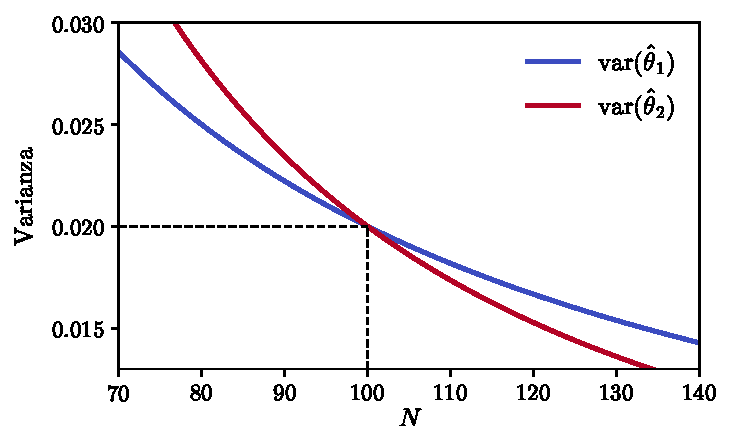
\includegraphics[width=\textwidth]{figuras/problem_7_4.pdf}
  \end{minipage}\hfill
  \begin{minipage}[c]{0.3\textwidth}
    \caption{
       Varianzas de los estimadores \(\hat{\theta}_1\) y \(\hat{\theta}_2\) en función de la cantidad de muestras \(N\). \(\var(\hat{\theta}_1)<\var(\hat{\theta}_2)\) si \(N<100\) y \(\var(\hat{\theta}_2)<\var(\hat{\theta}_1)\) si \(N>100\).
    } \label{fig:problem_7_4}
  \end{minipage}
\end{figure}

\subsection{Problema 5}\label{sec:problem_7_5}

Una definición formal de consistencia de un estimador es la siguiente. Un estimador \(\hat{\theta}\) es consistente si, dado \(\epsilon>0\),
\begin{equation}\label{eq:consistency_formal_definition}
 \lim_{N\to\infty}\Pr\{|\hat{\theta}-\theta|>\epsilon\}=0.
\end{equation}
Probar que la media muestral es un estimador consistente para el problema de la estimación del nivel \(A\) de DC en WGN con varianza conocida. Sugerencia: emplear la desigualdad de Chebychev.

\paragraph{Solución} Una secuencia de variables aleatorias \(\hat{\theta}\) que converge a \(\theta\) con \(N\) cumpliendo la ecuación \ref{eq:consistency_formal_definition}, se dice que \emph{converge en probabilidad} (ver el capítulo 7 de \cite{papoulis2002probability}). Por lo tanto, la definición de consistencia indica que el estimador \(\hat{\theta}\) es consistente si converge en probabilidad al valor verdadero \(\theta\) del parámetro. La desigualdad de Chebychev indica que si una variable aleatoria \(x\) tiene media \(\mu\) y varianza \(\sigma^2\), para todo \(\epsilon>0\) se cumple que (ver el capítulo 5 de \cite{papoulis2002probability})
\[
 \Pr\{|x-\mu|\geq\epsilon\}\leq\frac{\sigma^2}{\epsilon^2}.
\]
En el problema de la sección \ref{sec:problem_2_3} se mostró que la media muestral cumple que \(\bar{x}\sim\mathcal{N}(A,\,\sigma^2/N)\). Aplicando la desigualdad de Chebychev a \(\bar{x}\), se tiene que
\[
 \Pr\{|\bar{x}-A|\geq\epsilon\}\leq\frac{\sigma^2}{N\epsilon^2}.
\]
Por lo tanto, para todo \(\epsilon>0\) se cumple que
\[
 \lim_{N\to\infty}\Pr\{|\bar{x}-A|\geq\epsilon\}\leq\lim_{N\to\infty}\frac{\sigma^2}{N\epsilon^2}=0
\]
y por lo tanto, \(\bar{x}\) es consistente.

\subsection{Problema 6}

Otro resultado sobre consistencia establece que si \(\alpha=g(\theta)\) para una función \(g\) continua y \(\hat{\theta}\) es un estimador consistente de \(\theta\), se cumple que \(\hat{\alpha}=g(\hat{\theta})\) es un estimador consistente de \(\alpha\). Empleando el argumento de linealización estadística y la definición formal de consistencia, mostrar que la afirmación es cierta. Sugerencia: linealizar \(g\) en torno al valor verdadero de \(\theta\).

\paragraph{Solución} Hay que demostrar que
\[
 \lim_{N\to\infty}\Pr\{|\hat{\theta}-\theta|\geq\epsilon\}=0\qquad\Rightarrow\qquad
 \lim_{N\to\infty}\Pr\{|\hat{\alpha}-\alpha|\geq\epsilon\}=0.
\]
Sea \(\theta_0\) el valor verdadero del parámetro. Linealizando \(g\) en torno a \(\theta_0\) se tiene que
\[
 \alpha=g(\theta)\approx g(\theta_0)+\frac{dg}{d\theta}\bigg|_{\theta=\theta_0}(\theta-\theta_0).
\]
Por lo tanto,
\begin{align*}
 \hat{\alpha}-\alpha&\approx\left[g(\theta_0)+\frac{dg}{d\theta}\bigg|_{\theta=\theta_0}(\hat{\theta}-\theta_0)\right]-\left[g(\theta_0)+\frac{dg}{d\theta}\bigg|_{\theta=\theta_0}(\theta-\theta_0)\right]\\
  &=\frac{dg}{d\theta}\bigg|_{\theta=\theta_0}(\hat{\theta}-\theta).
\end{align*}
De esta forma
\begin{align*}
 \Pr\{|\hat{\alpha}-\alpha|\geq\epsilon\}&\approx\Pr\left\{\left|\frac{dg}{d\theta}\bigg|_{\theta=\theta_0}\right||\hat{\theta}-\theta|\geq\epsilon\right\}\\
  &=\Pr\left\{|\hat{\theta}-\theta|\geq\frac{\epsilon}{\left|\dfrac{dg}{d\theta}\bigg|_{\theta=\theta_0}\right|}\right\}\\
  &=\Pr\{|\hat{\theta}-\theta|\geq\epsilon'\}.
\end{align*}
Finalmente
\[
 \lim_{N\to\infty}\Pr\{|\hat{\alpha}-\alpha|\geq\epsilon\}=\lim_{N\to\infty}\Pr\{|\hat{\theta}-\theta|\geq\epsilon'\}=0,
\]
donde la segunda igualdad se cumple para todo \(\epsilon'>0\) debido a que \(\hat{\theta}\) es consistente y \(|dg/d\theta|_{\theta=\theta_0}|\) es finito por ser la función \(g\) continua. Se concluye que \(\hat{\alpha}\) es consistente.

\subsection{Problema 7}

Se consideran \(N\) observaciones IID de la familia de PDF exponenciales
\begin{equation}\label{eq:exponential_pdf_family}
 p(x;\,\theta)=\exp[A(\theta)B(x)+C(x)+D(\theta)]
\end{equation}
donde \(A\), \(B\), \(C\) y \(D\) son funciones de sus respectivos argumentos. Encontrar la ecuación a resolver para encontrar el MLE. Aplicar los resultados a las PDF del problema de la sección \ref{sec:problem_7_3}.

\paragraph{Solución} La PDF de los datos es
\begin{align*}
 p(\x;\,\theta)&=\prod_{n=0}^{N-1}\exp[A(\theta)B(x[n])+C(x[n])+D(\theta)]\\
  &=\exp\left[A(\theta)\sum_{n=0}^{N-1}B(x[n])+\sum_{n=0}^{N-1}C(x[n])+ND(\theta)\right],
\end{align*}
y su máximo se obtiene maximizando
\[
 J(\theta)=A(\theta)\sum_{n=0}^{N-1}B(x[n])+\sum_{n=0}^{N-1}C(x[n])+ND(\theta).
\]
La derivada respecto al parámetro es
\[
 \frac{\partial J(\theta)}{\partial\theta}=A'(\theta)\sum_{n=0}^{N-1}B(x[n])+ND'(\theta),
\]
e igualando a cero, se obtiene que el MLE \(\hat{\theta}\) cumple que
\begin{equation}\label{eq:exponential_pdf_family_mle}
 A'(\hat{\theta})\sum_{n=0}^{N-1}B(x[n])+ND'(\hat{\theta})=0.
\end{equation}

Se aplicará el resultado para encontrar el MLE de las PDF de la familia exponencial del problema de la sección \ref{sec:problem_7_3}.
\begin{enumerate}[a.]
 \item Gaussiana
 \begin{align*}
  p(x;\,\mu)&=\frac{1}{\sqrt{2\pi}}\exp\left[-\frac{1}{2}(x-\mu)^2\right]\\
    &=\exp\left[-\frac{1}{2}\ln2\pi-\frac{x^2}{2}+x\mu-\frac{\mu^2}{2}\right].
 \end{align*}
 Por lo tanto, asociando términos con la ecuación \ref{eq:exponential_pdf_family}, se tiene que
 \[
  A(\mu)=\mu,\qquad B(x)=x,\qquad C(x)=-\frac{1}{2}\ln2\pi-\frac{x^2}{2},\qquad
   D(\mu)=-\frac{\mu^2}{2}.
 \]
 y aplicando la ecuación \ref{eq:exponential_pdf_family_mle}, el MLE cumple que
 \[
  1\times\sum_{n=0}^{N-1}x[n]-N\hat{\mu}=0,
 \]
 concluyendo que
 \[
  \hat{\mu}=\frac{1}{N}\sum_{n=0}^{N-1}x[n]=\bar{x}.
 \]
 \item Exponencial. Si \(x>0\),
\begin{align*}
 p(x;\,\lambda)&=\lambda\exp(-\lambda x)\\
  &=\exp(\ln\lambda-\lambda x),
\end{align*}
 y asociando términos con la ecuación \ref{eq:exponential_pdf_family}, se tiene que
 \[
  A(\mu)=-\lambda,\qquad B(x)=x,\qquad C(x)=0,\qquad D(\lambda)=\ln\lambda.
 \]
 Aplicando la ecuación \ref{eq:exponential_pdf_family_mle}, el MLE cumple que
 \[
  -1\times\sum_{n=0}^{N-1}x[n]+N\times\frac{1}{\hat{\lambda}}=0
 \]
 concluyendo que
 \[
  \hat{\lambda}=\frac{1}{\displaystyle\frac{1}{N}\sum_{n=0}^{N-1}x[n]}=\frac{1}{\bar{x}}.
 \]
\end{enumerate}

\subsection{Problema 8}

Si se observan \(N\) muestras IID de un experimento Bernoulli (tirar una moneda) con probabilidades
\[
 \begin{array}{lcl}
  \Pr\{x[n]=1\} & = & p\\
  \Pr\{x[n]=0\} & = & 1-p
 \end{array}
\]
encontrar el MLE.

\paragraph{Solución} Teniendo en cuenta que la PDF de una muestra es
\[
 p(x[n];\,p)=p^{x[n]}(1-p)^{1-x[n]},
\]
la PDF de los datos es
\begin{align*}
 p(\x,\,p)&=\prod_{n=0}^{N-1}p^{x[n]}(1-p)^{1-x[n]}\\
  &=p^{\sum_{n=0}^{N-1}x[n]}(1-p)^{N-\sum_{n=0}^{N-1}x[n]}.
\end{align*}
La derivada respecto al parámetro es
\begin{align*}
 \frac{\partial p(\x,\,p)}{\partial p}&=\left(\sum_{n=0}^{N-1}x[n]\right)p^{\left(\sum_{n=0}^{N-1}x[n]\right)-1}(1-p)^{N-\sum_{n=0}^{N-1}x[n]}\\
  &\qquad-p^{\sum_{n=0}^{N-1}x[n]}\left(N-\sum_{n=0}^{N-1}x[n]\right)(1-p)^{N-1-\sum_{n=0}^{N-1}x[n]}\\
  &=p^{\left(\sum_{n=0}^{N-1}x[n]\right)-1}(1-p)^{N-1-\sum_{n=0}^{N-1}x[n]}
   \left[\left(\sum_{n=0}^{N-1}x[n]\right)(1-p)-p\left(N-\sum_{n=0}^{N-1}x[n]\right)\right],
\end{align*}
e igualando a cero, el MLE cumple que
\[
 \left(\sum_{n=0}^{N-1}x[n]\right)(1-\hat{p})-\hat{p}\left(N-\sum_{n=0}^{N-1}x[n]\right)=0,
\]
es decir
\[
 \hat{p}=\frac{1}{N}\sum_{n=0}^{N-1}x[n]=\bar{x}.
\]


\subsection{Problema 9}

Para \(N\) observaciones IID de una PDF \(\mathcal{U}[0,\,\theta]\), encontrar el MLE de \(\theta\).

\paragraph{Solución} La PDF de una muestra es
\[
\def\arraystretch{1.4}
 p(x[n];\,\theta)=
 \left\{\begin{array}{ll}
  \dfrac{1}{\theta}, &  x[n]\in[0,\,\theta]\\
  0, &  \textrm{en otro caso}
 \end{array}\right.
\]
y la PDF de los datos es
\[
\def\arraystretch{1.4}
 p(\x;\,\theta)=
 \left\{\begin{array}{ll}
  \dfrac{1}{\theta^N}, &  x[0]\in[0,\,\theta],\,\dots,\,x[N-1]\in[0,\,\theta]\\
  0, &  \textrm{en otro caso}.
 \end{array}\right.
\]
Se observa que la función de verosimilitud no es acotada, ya que
\[
 \lim_{\theta\to0}p(\x;\,\theta)=\lim_{\theta\to0}\frac{1}{\theta^N}=\infty.
\]
Por lo tanto, la función se maximiza cuando \(\theta\) es lo mas pequeño posible. Como se cumple que \(\theta>x[n]\) para \(n=0,\,\dots,\,N-1\), el valor mas pequeño posible es \(\theta_\textrm{min}=\max x[n]\). De esta forma, el MLE es
\[
 \hat{\theta}=\max x[n].
\]

\subsection{Problema 10}

Si se observa el conjunto de datos
\[
 x[n]=As[n]+w[n],\qquad n=0,\,\dots,\,N-1,
\]
donde \(s[n]\) es conocida y \(w[n]\) es WGN de varianza \(\sigma^2\) conocida, encontrar el MLE de \(A\). Determinar la PDF del MLE y si se verifica la PDF asintótica del MLE.

\paragraph{Solución} La PDF de los  datos es
\[
 p(\x,\,A)=\frac{1}{(2\pi\sigma^2)^\frac{N}{2}}\exp\left[-\frac{1}{2\sigma^2}\sum_{n=0}^{N-1}(x[n]-As[n])^2\right].
\]
Para maximizar la función de verosimilitud, hay que minimizar el exponente
\[
 J(A)=\sum_{n=0}^{N-1}(x[n]-As[n])^2.
\]
La derivada es
\[
 \frac{\partial J(A)}{\partial A}=\sum_{n=0}^{N-1}2(x[n]-As[n])(-s[n]).
\]
e igualando a cero, el MLE cumple que
\[
 \sum_{n=0}^{N-1}(x[n]-\hat{A}s[n])s[n]=0
\]
es decir,
\[
 \hat{A}=\frac{\displaystyle\sum_{n=0}^{N-1}x[n]s[n]}{\displaystyle\sum_{n=0}^{N-1}s^2[n]}.
\]
Además, \(\hat{A}\) es gaussiana por ser la combinación lineal de variables aleatorias gaussianas.
La media de \(\hat{A}\) es
\[
 E(\hat{A})=\frac{\displaystyle\sum_{n=0}^{N-1}E(x[n])s[n]}{\displaystyle\sum_{n=0}^{N-1}s^2[n]}
  \overset{(a)}{=}\frac{\displaystyle A\sum_{n=0}^{N-1}s^2[n]}{\displaystyle\sum_{n=0}^{N-1}s^2[n]}=A,
\]
donde en \((a)\) se consideró que \(E(x[n])=As[n]\). La varianza de \(\hat{A}\) es
\[
 \var(\hat{A})=\frac{\displaystyle\sum_{n=0}^{N-1}\var(x[n])s^2[n]}{\left(\displaystyle\sum_{n=0}^{N-1}s^2[n]\right)^2}
 =\frac{\displaystyle\sigma^2\sum_{n=0}^{N-1}s^2[n]}{\left(\displaystyle\sum_{n=0}^{N-1}s^2[n]\right)^2}
 =\frac{\sigma^2}{\displaystyle\sum_{n=0}^{N-1}s^2[n]}=\frac{\sigma^2}{\s^T\s}\overset{(a)}{=}I^{-1}(A),
\]
donde en \((a)\) se notó que el modelo de los datos de este problema es un caso particular del modelo lineal (ecuación \ref{eq:linear_model}) con \(\thetabf=A\) y \(\Hbf=\s\), por lo que el lado izquierdo de la igualdad es el inverso de la información de Fisher del parámetro, como indica la ecuación \ref{eq:linear_model_fisher}.
Se concluye que la PDF del MLE es
\[
 \hat{A}\sim\mathcal{N}\left(A,\,I^{-1}(A)\right),
\]
que coincide con la PDF asintótica del MLE pero en este caso es válido para un número finito de muestras.


\subsection{Problema 11}\label{sec:problem_7_11}

Encontrar la ecuación a resolver para el MLE del coeficiente de correlación \(\rho\) en el problema de la sección \ref{sec:problem_3_15}. Encontrar una solución aproximada cuando \(N\to\infty\). Sugerencia: notar que \(\sum_{n=0}^{N-1}x_0^2[n]/N\to1\) y \(\sum_{n=0}^{N-1}x_1^2[n]/N\to1\) donde \(\x[n]=[x_0[n]\;x_1[n]]\).

\paragraph{Solución} Hay que maximizar la función de verosimilitud. Como el logaritmo es una función monotonamente creciente, es equivalente maximizar la función de verosimilitud logarítmica. La derivada de la función logarítmica se calculó en el problema de la sección \ref{sec:problem_3_15} y está dada por la ecuación \ref{eq:problem_3_15_likelihood_pdf},
\[
 \dfrac{\partial\ln p(\x;\,\rho)}{\partial\rho}=\frac{N\rho}{(1-\rho^2)}+\frac{1}{(1-\rho^2)^2}\sum_{n=0}^{N-1}\left[(1+\rho^2)x_0[n]x_1[n]-\rho(x_0^2[n]+x_1^2[n])\right].
\]
Igualando a cero, se obtiene que el MLE de \(\rho\) cumple que
\[
 \frac{N\hat{\rho}}{(1-\hat{\rho}^2)}+\frac{1}{(1-\hat{\rho}^2)^2}\sum_{n=0}^{N-1}\left[(1+\hat{\rho}^2)x_0[n]x_1[n]-\hat{\rho}(x_0^2[n]+x_1^2[n])\right]=0,
\]
o
\[
 \hat{\rho}(1-\hat{\rho}^2)+(1+\hat{\rho}^2)\frac{1}{N}\sum_{n=0}^{N-1}x_0[n]x_1[n]-\hat{\rho}\left(\frac{1}{N}\sum_{n=0}^{N-1}x_0^2[n]+\frac{1}{N}\sum_{n=0}^{N-1}x_1^2[n]\right)=0.
\]
Cuando \(N\to\infty\), por la ley de los grandes números, se cumple que
\[
 \frac{1}{N}\sum_{n=0}^{N-1}x_0^2[n]\to E(x_0^2[n])=\var(x_0[n])=1,\qquad\qquad
 \frac{1}{N}\sum_{n=0}^{N-1}x_1^2[n]\to E(x_1^2[n])=\var(x_1[n])=1,
\]
por lo que la condición del MLE se puede aproximar como
\[
 \hat{\rho}(1-\hat{\rho}^2)+(1+\hat{\rho}^2)\frac{1}{N}\sum_{n=0}^{N-1}x_0[n]x_1[n]-2\hat{\rho}=0.
\]
Definiendo \(\hat{C}_{12}=\sum_{n=0}^{N-1}x_0[n]x_1[n]/N\) y operando, se tiene que
\[
 \hat{\rho}-\hat{\rho}^3+\hat{C}_{12}+\hat{C}_{12}\hat{\rho}^2-2\hat{\rho}=0\qquad\qquad\Rightarrow\qquad\qquad
 \hat{\rho}^3-\hat{C}_{12}\hat{\rho}^2+\hat{\rho}-\hat{C}_{12}=0.
\]
Observando que el polinomio se puede escribir como
\[
 \hat{\rho}^2(\hat{\rho}-\hat{C}_{12})+(\hat{\rho}-\hat{C}_{12})=0\qquad\qquad\Rightarrow\qquad\qquad
 (\hat{\rho}^2+1)(\hat{\rho}-\hat{C}_{12})=0,
\]
se concluye que
\[
 \hat{\rho}=\hat{C}_{12}=\frac{1}{N}\sum_{n=0}^{N-1}x_0[n]x_1[n].
\]

\subsection{Problema 12}\label{sec:problem_7_12}

En este problema se prueba que si existe un estimador eficiente, el método de máxima verosimilitud lo obtiene. Asumiendo un parámetro escalar, si existe un estimador eficiente, se cumple que
\[
 \dfrac{\partial\ln p(\x;\,\rho)}{\partial\rho}=I(\theta)(\hat{\theta}-\theta).
\]
Usar esto para probar el teorema.

\paragraph{Solución} Maximizar la función de verosimilitud es equivalente a maximizar la función de verosimilitud logarítmica. Asumiendo que \(I(\theta)>0\) para todo \(\theta\), ya que de lo contrario la PDF no dependería del parámetro, el MLE cumple que
\[
 I(\theta_\textrm{MLE})(\hat{\theta}-\theta_\textrm{MLE})=0
\]
y por lo tanto,
\[
 \theta_\textrm{MLE}=\hat{\theta},
\]
donde \(\hat{\theta}\) es el estimador eficiente.

\subsection{Problema 13}

Se observan N muestras IID del nivel de continua en WGN de varianza conocida \(\sigma^2\). Mediante una simulación por computadora, verificar que la PDF del MLE o la media muestral es \(\mathcal{N}(0,\,\sigma^2/N)\). Graficar las PDFs teórica y la obtenida mediante la simulación. Usar \(A=1\), \(\sigma^2=0.1\), \(N=50\) y \(M=1000\) realizaciones. ¿Qué ocurre si \(M\) se incrementa a 5000?

\paragraph{Solución} Con los valores indicados, la PDF teórica de la media muestral es \(\mathcal{N}(1,\,0.002)\). Se realizó una simulación por computadora repitiendo la estimación \(M=1000\) y \(M=10000\) veces. El resultado se muestra en la figura \ref{fig:problem_7_13}. Se observa que al incrementar la cantidad de realizaciones, la PDF experimental se ajusta mas a la PDF teórica.
\begin{figure}[!htb]
\begin{center}
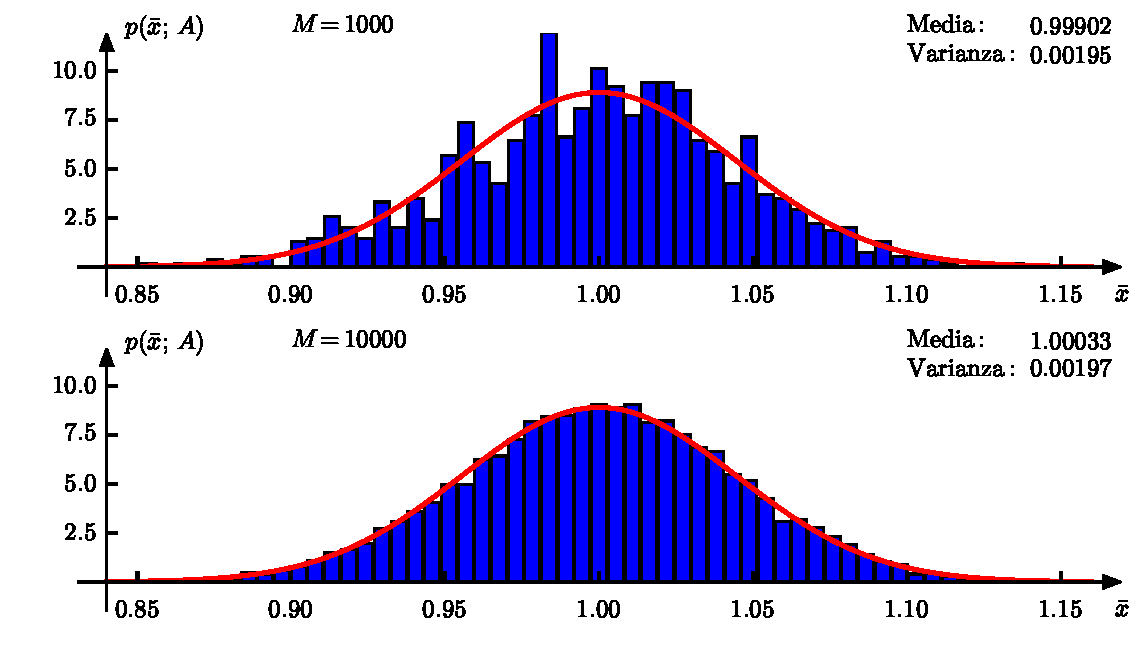
\includegraphics[width=\textwidth]{figuras/problem_7_13.pdf}
\caption{\label{fig:problem_7_13} PDF teórica y experimental del MLE. La PDF teórica (en rojo) es \(\mathcal{N}(1,\,0.002)\).}
\end{center}
\end{figure}

\subsection{Problema 14} 

Se consideran los datos \(x[n]\) IID para \(n=0,\,\dots,\,N-1\), con \(x[n]\sim\mathcal{N}(0,\,\sigma^2)\). De acuerdo al teorema de Slutsky, si \(\bar{x}\) es la media muestral y
\[
 \hat{\sigma^2}=\frac{1}{N}\sum_{n=0}^{N-1}(x[n]-\bar{x})^2
\]
es la varianza muestral, se cumple que
\[
 \frac{\bar{x}}{\hat{\sigma}/\sqrt{N}}\overset{a}{\sim}\mathcal{N}(0,\,1).
\]
Si bien esto puede ser probado analíticamente, requiere familiaridad con el concepto de convergencia de variables aleatorias. En lugar de ello, implementar una simulación por computadora para encontrar la PDF de \(\bar{x}/(\hat{\sigma}/\sqrt{N})\) para \(\sigma^2=1\) y \(N=10\) y \(N=100\). Comparar el resultado con la PDF asintótica teórica.

\paragraph{Solución} Se realizará primero un esbozo de la demostración analítica para el caso en que \(x[n]\) son IID con \(E(x[n])=\mu\) y \(\var(x[n])=\sigma^2\) pero con PDF arbitraria. En ese caso,
\[
 \frac{\bar{x}-\mu}{\hat{\sigma}/\sqrt{N}}\overset{d}{\longrightarrow}\mathcal{N}(0,\,1).
\]
La notación significa convergencia en distribución.
Para mostrarlo, se considera primero la variable aleatoria \(\sqrt{N}(\bar{x}-\mu)\). Como \(E[\sqrt{N}(\bar{x}-\mu)]=0\) y \(\var[\sqrt{N}(\bar{x}-\mu)]=\sigma^2\), por el teorema central del límite clásico\footnote{Ver \url{https://en.wikipedia.org/wiki/Central_limit_theorem\#Classical_CLT}, por ejemplo.}, se cumple que con \(N\to\infty\)
\[
 \sqrt{N}(\bar{x}-\mu)\overset{d}{\longrightarrow}x\sim\mathcal{N}\left(0,\,\sigma^2\right).
\]
Por otro lado, operando con la varianza muestral, se ve que
\begin{align*}
 \hat{\sigma^2}&=\frac{1}{N}\sum_{n=0}^{N-1}(x[n]-\bar{x})^2\\
  &=\frac{1}{N}\sum_{n=0}^{N-1}[(x[n]-\mu)-(\bar{x}-\mu)]^2\\
  &=\frac{1}{N}\sum_{n=0}^{N-1}(x[n]-\mu)^2-\frac{1}{N}\sum_{n=0}^{N-1}2(\bar{x}-\mu)(x[n]-\mu)+\frac{1}{N}\sum_{n=0}^{N-1}(\bar{x}-\mu)^2\\
  &=\frac{1}{N}\sum_{n=0}^{N-1}(x[n]-\mu)^2-2(\bar{x}-\mu)\frac{1}{N}\sum_{n=0}^{N-1}(x[n]-\mu)+(\bar{x}-\mu)^2\\
  &=\frac{1}{N}\sum_{n=0}^{N-1}(x[n]-\mu)^2-2(\bar{x}-\mu)\left(\frac{1}{N}\sum_{n=0}^{N-1}x[n]-\mu\right)+(\bar{x}-\mu)^2,
\end{align*}
resultando en
\[
 \hat{\sigma^2}=\frac{1}{N}\sum_{n=0}^{N-1}(x[n]-\mu)^2-(\bar{x}-\mu)^2.
\]
Por la ley de los grandes números, se cumple que
\[
 \bar{x}\overset{a.s.}{\longrightarrow}E(x[n])=\mu\qquad\qquad\textrm{y}\qquad\qquad
 \frac{1}{N}\sum_{n=0}^{N-1}(x[n]-\mu)^2\overset{a.s.}{\longrightarrow}E[(x[n]-\mu)^2]=\sigma^2,
\]
y por lo tanto,
\[
 \hat{\sigma^2}\overset{a.s.}{\longrightarrow}\sigma^2.
\]
La notación significa convergencia casi segura, como indica la ley fuerte de los grandes números. En la ley débil de los grandes números, la convergencia es en probabilidad. Pero como convergencia casi segura implica convergencia en probabilidad (ver el capítulo 7 de \cite{papoulis2002probability}), en cualquier caso se cumple que
\[
 \hat{\sigma^2}\overset{p}{\longrightarrow}\sigma^2.
\]
Finalmente, empleando el teorema de Slutsky, referido previamente en este capítulo, se tiene que
\[
\begin{array}{rcl}
 \sqrt{N}(\bar{x}-\mu)&\overset{d}{\longrightarrow}&x\sim\mathcal{N}\left(0,\,\sigma^2\right)\\
 \hat{\sigma^2}&\overset{p}{\longrightarrow}&\sigma^2
\end{array}
\qquad\Rightarrow\qquad
 \frac{\sqrt{N}(\bar{x}-\mu)}{\hat{\sigma}}\overset{d}{\longrightarrow}\frac{x}{\sigma}\sim\mathcal{N}(0,\,1).
\]

Se realizó una simulación por computadora calculando \(\sqrt{N}\bar{x}/\hat{\sigma}\) con valores de \(N=10\) y \(N=1000\) una cantidad \(M=1000\) veces. Los resultados de muestran en la figura \ref{fig:problem_7_14}, comparando el histograma de los valores prácticos con la PDF teórica \(\mathcal{N}(0,\,1)\). Como es de esperar, cuando mayor es \(N\) mejor es la aproximación al resultado asintótico teórico. Se observa que con \(N=10\) hay una diferencia considerable fundamentalmente en la varianza.
\begin{figure}[!htb]
\begin{center}
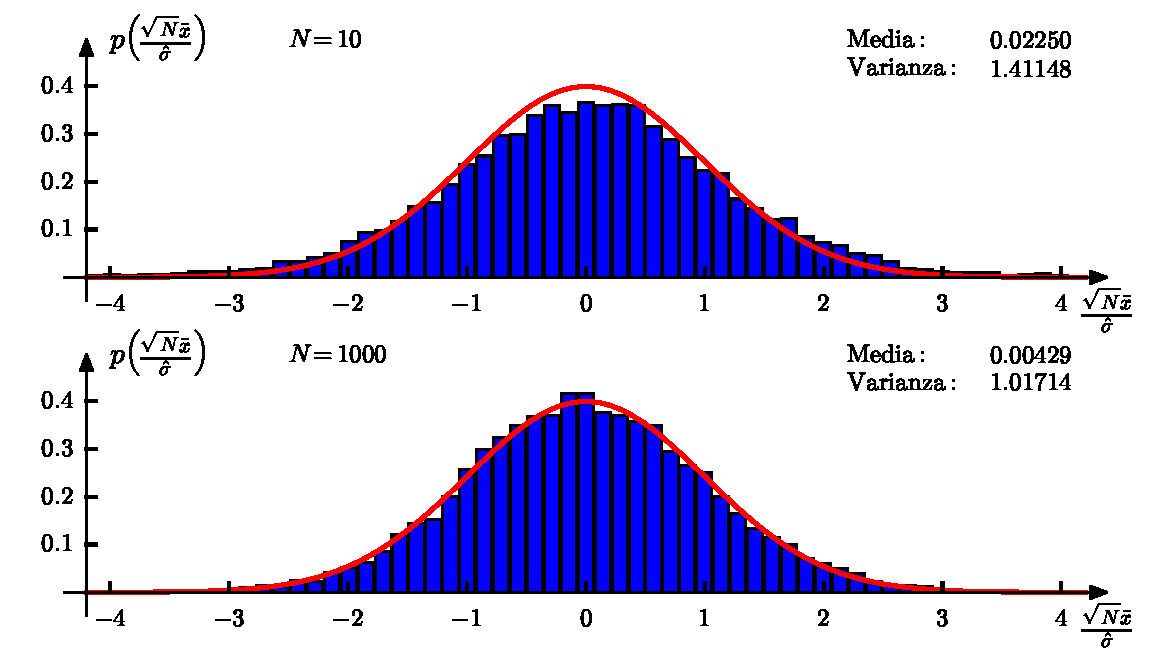
\includegraphics[width=\textwidth]{figuras/problem_7_14.pdf}
\caption{\label{fig:problem_7_14} PDF teórica y experimental de \(\sqrt{N}\bar{x}/\hat{\sigma}\). La PDF teórica (en rojo) es \(\mathcal{N}(0,\,1)\). Cuando \(N\) es pequeño, la varianza experimental es considerablemente mayor que la varianza asintótica teórica.}
\end{center}
\end{figure}

\subsection{Problema 15}\label{sec:problem_7_15}

En este problema se muestra que el MLE alcanza la PDF asintótica cuando el error de estimación es pequeño. Se considera el ejemplo de la sección \ref{sec:mle_sinusoidal_phase} del MLE de la fase de una sinusoide y sea 
\[
\def\arraystretch{2.8}
 \begin{array}{rcl}
  \epsilon_s&=&\displaystyle-\frac{2}{NA}\sum_{n=0}^{N-1}w[n]\sin2\pi f_0n\\
  \epsilon_c&=&\displaystyle\frac{2}{NA}\sum_{n=0}^{N-1}w[n]\cos2\pi f_0n
 \end{array}
\]
en la ecuación \ref{eq:mle_sinusoidal_parameters_phi_estimator_alt}. Se asume que \(f_0\) no es cercano a 0 ni a 1/2 de forma que se pueden realizar las aproximaciones del problema \ref{sec:problem_3_7}. Probar primero que \(\epsilon_s\) y \(\epsilon_c\) son variables aleatorias gaussianas aproximadamente no correlacionadas y por lo tanto independientes. Además, determinar la PDF de \(\epsilon_s\) y \(\epsilon_c\). Luego, asumiendo que \(\epsilon_s\) y \(\epsilon_c\) son pequeños, emplear una expansión en series de Taylor de \(\hat{\phi}\) en torno al valor verdadero \(\phi\),
\begin{align*}
 \hat{\phi}&=g(\epsilon_s,\,\epsilon_c)\\
  &\approx g(0,\,0)+\frac{\partial g(\epsilon_s,\,\epsilon_c)}{\partial\epsilon_s}\bigg|_{\epsilon_s=0,\,\epsilon_c=0}\epsilon_s+\frac{\partial g(\epsilon_s,\,\epsilon_c)}{\partial\epsilon_c}\bigg|_{\epsilon_s=0,\,\epsilon_c=0}\epsilon_c,
\end{align*}
donde la función \(g\) esta dada por la ecuación \ref{eq:mle_sinusoidal_parameters_phi_estimator_alt}. Usar esta expansión para encontrar la PDF de \(\hat{\phi}\). Comparar la varianza con la CRLB calculada en el ejemplo 3.4. Notar que para que \(\epsilon_s\) y \(\epsilon_c\) sean pequeños, se debe cumplir que \(N\to\infty\) y/o \(A\to\infty\).

\paragraph{Solución} La ecuación \ref{eq:mle_sinusoidal_parameters_phi_estimator_alt} expresada en función los términos de error \(\epsilon_s\) y \(\epsilon_c\) es
\[
 \hat{\phi}\approx\arctan\frac{\sin\phi+\epsilon_s}{\cos\phi+\epsilon_s}.
\]
Se probará primero que \(\epsilon_s\) y \(\epsilon_c\) son aproximadamente no correlacionadas, es decir, que se cumple que
\[
 \cov(\epsilon_s,\,\epsilon_c)=E(\epsilon_s\epsilon_c)-E(\epsilon_s)E(\epsilon_c)=0.
\]
Teniendo en cuenta que \(E(\epsilon_s)=E(\epsilon_c)=0\), se tiene que
\begin{align*}
 \cov(\epsilon_s,\,\epsilon_c)&=E(\epsilon_s\epsilon_c)\\
  &=-\frac{4}{N^2A^2}\sum_{m=0}^{N-1}\sum_{n=0}^{N-1}E(w[m]w[n])\sin(2\pi f_0m)\cos(2\pi f_0n)\\
  &=-\frac{4\sigma^2}{N^2A^2}\sum_{n=0}^{N-1}\sin(2\pi f_0n)\cos(2\pi f_0n),
\end{align*}
donde en la última igualdad se empleó que las muestras \(w[n]\) de ruido son independientes y por lo tanto
\begin{equation}\label{eq:problem_7_15_independent_noise}
  E(w[m]w[n])=
 \left\{
 \begin{array}{lc}
  \sigma^2, & m=n\\
  0, & m\neq n
 \end{array}\right.
 =\sigma^2\delta[m-n].
\end{equation}
Considerando la identidad trigonométrica \(\sin2\theta=2\sin\theta\cos\theta\) y empleando la aproximación demostrada en el problema de la sección \ref{sec:problem_3_7}, se obtiene que
\[
 \cov(\epsilon_s,\,\epsilon_c)=-\frac{2\sigma^2}{N^2A^2}\sum_{n=0}^{N-1}\sin4\pi f_0n\approx0,
\]
concluyendo que \(\epsilon_s\) y \(\epsilon_c\) son aproximadamente no correlacionadas. Además, son variables aleatorias gaussianas por ser una combinación lineal de variables aleatorias gaussianas independientes. Finalmente, por ser aproximadamente no correlacionadas y gaussianas, \(\epsilon_s\) y \(\epsilon_c\) son aproximadamente independientes. Para calcular su PDF solo falta calcular las varianzas. Procediendo de forma análoga al cálculo de la covarianza, se tiene que
\begin{align*}
 \var(\epsilon_s)&=E(\epsilon_s^2)\\
  &\overset{(a)}{=}\frac{4\sigma^2}{N^2A^2}\sum_{n=0}^{N-1}\sin^22\pi f_0n\\
  &\overset{(b)}{=}\frac{2\sigma^2}{N^2A^2}\left(N-\sum_{n=0}^{N-1}\cos4\pi f_0n\right)\\
  &\overset{(c)}{\approx}\frac{2\sigma^2}{NA^2},
\end{align*}
donde en \((a)\) se empleó la ecuación \ref{eq:problem_7_15_independent_noise} en \((b)\) se empleó la identidad trigonométrica \(2\sin^{2}\theta=1-\cos2\theta\) y en \((c)\) la aproximación demostrada en el problema \ref{sec:problem_3_7}. Analogamente,
\begin{align*}
 \var(\epsilon_c)&=E(\epsilon_c^2)\\
  &=\frac{4\sigma^2}{N^2A^2}\sum_{n=0}^{N-1}\cos^22\pi f_0n\\
  &\overset{(a)}{=}\frac{2\sigma^2}{N^2A^2}\left(N+\sum_{n=0}^{N-1}\cos4\pi f_0n\right)\\
  &\approx\frac{2\sigma^2}{NA^2},
\end{align*}
donde en \((a)\) se empleó la identidad trigonométrica \(2\cos^{2}\theta=1+\cos2\theta\). Se concluye que
\[
 \epsilon_s,\,\epsilon_c\sim\mathcal{N}\left(0,\,\frac{2\sigma^2}{NA^2}\right).
\]
Se aproximará el estimador mediante la serie de Taylor indicada. Como
\[
 g(\epsilon_s,\,\epsilon_c)=\arctan\frac{\sin\phi+\epsilon_s}{\cos\phi+\epsilon_c},
\]
y \(d\arctan x/dx=1/(1+x^2)\), se tiene que
\[
 \frac{\partial g(\epsilon_s,\,\epsilon_c)}{\partial\epsilon_s}=
 \frac{1}{1+\left(\dfrac{\sin\phi+\epsilon_s}{\cos\phi+\epsilon_c}\right)^2}
 \frac{1}{\cos\phi+\epsilon_c}
 \qquad\textrm{y}\qquad
 \frac{\partial g(\epsilon_s,\,\epsilon_c)}{\partial\epsilon_c}=
 -\frac{1}{1+\left(\dfrac{\sin\phi+\epsilon_s}{\cos\phi+\epsilon_c}\right)^2}
 \frac{\sin\phi+\epsilon_s}{(\cos\phi+\epsilon_c)^2}.
\]
Además, \(g(0,\,0)=\phi\),
\[
  \frac{\partial g(\epsilon_s,\,\epsilon_c)}{\partial\epsilon_s}\bigg|_{\epsilon_s=0,\,\epsilon_c=0}
  =\frac{1}{1+\dfrac{\sin^2\phi}{\cos^2\phi}}
 \frac{1}{\cos\phi}=\cos\phi
\]
y
\[
 \frac{\partial g(\epsilon_s,\,\epsilon_c)}{\partial\epsilon_c}\bigg|_{\epsilon_s=0,\,\epsilon_c=0}=
 -\frac{1}{1+\dfrac{\sin^2\phi}{\cos^2\phi}}
 \frac{\sin\phi}{\cos^2\phi}
 =-\sin\phi.
\]
Sustituyendo estos resultados en la serie de Taylor se concluye que
\[
 \hat{\phi}\approx\phi+\epsilon_s\cos\phi-\epsilon_c\sin\phi.
\]
Para encontrar la PDF de \(\hat{\phi}\), se observa que se trata de una variable aleatoria gaussiana por ser la combinación lineal de dos variables aleatorias gaussianas independientes. Además, \(E(\hat{\phi})=\phi\) y 
\begin{align*}
 \var(\hat{\phi})&\overset{(a)}{=}\var(\epsilon_s)\cos^2\phi+\var(\epsilon_c)\sin^2\phi\\
  &=\frac{2\sigma^2}{NA^2}\left(\cos^2+\sin^2\right)\\
  &=\frac{2\sigma^2}{NA^2},
\end{align*}
donde en \((a)\) se tuvo en cuenta que \(\epsilon_s\) y \(\epsilon_c\) son independientes. Se concluye que
\[
 \hat{\phi}\sim\mathcal{N}\left(\phi,\,\frac{2\sigma^2}{NA^2}\right).
\]
En el ejemplo de la sección \ref{sec:crlb_sinusoidal_phase} se demuestra que la CRLB de \(\phi\) es
\[
 \var(\hat{\phi})\geq\frac{2\sigma^2}{NA^2}.
\]
Por lo tanto, el MLE alcanza aproximadamente la CRLB.

\subsection{Problema 16}\label{sec:problem_7_16}

Para el ejemplo de la sección \ref{sec:mle_dc_level_correlated_non_gaussian}, determinar la \(\var(\hat{A})\) así como la CRLB para el ruido de PDF de Laplace
\[
 p(w[0])=\frac{1}{2}e^{-|w[n]|}
\]
¿El MLE alcanza la CRLB cuando \(N\to\infty\)?

\paragraph{Solución} Como se indica en el ejemplo, la varianza del MLE es
\[
 \var(\hat{A})=\int_{-\infty}^{\infty}u^2p(u)\,du,
\]
y con \(w[n]\) con PDF de Laplace queda
\begin{align*}
 \var(\hat{A})&=\frac{1}{2}\int_{-\infty}^{\infty}u^2e^{-|u|}\,du\\
  &=\int_{0}^{\infty}u^2e^{-u}\,du\\
  &\overset{(a)}{=}-u^2e^{-u}\bigg|_{0}^{\infty}-2\int_{0}^{\infty}ue^{-u}\,du\\
  &\overset{(b)}{=}2\left(ue^{-u}\bigg|_{0}^{\infty}+\int_{0}^{\infty}e^{-u}\,du\right)\\
  &=-2e^{-u}\bigg|_{0}^{\infty}\\
  &=2,
\end{align*}
donde en \((a)\) se aplicó integración por partes \(\int xdy=xy-\int ydx\) con \(x=u^2\) y \(dy=e^{-u}\,du\) y por lo tanto, \(dx=2u\,du\) y \(y=-e^{-u}\) y en \((b)\) se tuvo en cuenta que el primer término es nulo y nuevamente se aplicó integración por partes en la integral con \(x=u\) y \(dy=-e^{-u}\,du\) y por lo tanto, \(dx=du\) y \(y=e^{-u}\). Por otro lado, la CRLB es (ver el problema \ref{sec:problem_3_2})
\[
 \var(\hat{A})\geq\left[\int_{-\infty}^{\infty}\frac{\left(\dfrac{dp_{w[0]}(u)}{du}\right)^2}{p_{w[0]}(u)}\,du\right]^{-1}.
\]
Teniendo en cuenta que en este caso
\[
\def\arraystretch{2.2}
\frac{dp_{w[0]}(u)}{du}=
\left\{
 \begin{array}{ll}
  -\dfrac{1}{2}e^{-u},&u>0\\
  \dfrac{1}{2}e^{u},&u<0
 \end{array}\right.
 \qquad\Rightarrow\qquad
\left(\dfrac{dp_{w[0]}(u)}{du}\right)^2=
\left\{
 \begin{array}{ll}
  \dfrac{1}{4}e^{-2u},&u>0\\
  \dfrac{1}{4}e^{2u},&u<0
 \end{array}\right. 
 =\dfrac{1}{4}e^{-2|u|},
\]
la CRLB queda
\begin{align*}
 \var(\hat{A})&\geq\left[\int_{-\infty}^{\infty}\frac{\dfrac{1}{4}e^{-2|u|}}{\dfrac{1}{2}e^{-|u|}}\,du\right]^{-1}\\
  &\overset{(a)}{=}\left[2\int_{0}^{\infty}\frac{\dfrac{1}{4}e^{-2u}}{\dfrac{1}{2}e^{-u}}\,du\right]^{-1}\\
  &=\left[\int_{0}^{\infty}e^{-u}\,du\right]^{-1}\\
  &=1,
\end{align*}
donde en \((a)\) se consideró que tanto el numerador como el denominador del integrando son funciones pares resultando en una función par. Se obtuvo que \(\var(\hat{A})=2\) mientras que \(\operatorname{CRLB}(A)=1\). Además, como la varianza del MLE es constante con \(N\), no se cumple que el MLE alcance la CRLB con \(N\to\infty\).

\subsection{Problema 17}

Para \(N\) observaciones IID de una PDF \(\mathcal{N}(0,\,1/\theta)\) donde \(\theta>0\), encontrar el MLE de \(\theta\) y su PDF asintótica.

\paragraph{Solución} El MLE de \(\theta\) puede obtenerse maximizando \(p(\x;\,\theta)\), donde
\[
 p(\x;\,\theta)=\left(\frac{\theta}{2\pi}\right)^\frac{N}{2}\exp\left(-\frac{\theta}{2}\sum_{n=0}^{N-1}x^2[n]\right),
\]
pero el problema se resolverá considerando que las observaciones tienen PDF \(\mathcal{N}(0,\,\sigma^2)\), buscando el MLE de \(\sigma^2\) y luego empleando la propiedad de invarianza ante transformaciones del MLE (sección \ref{sec:mle_invariance_property}) que establece que el MLE de \(\theta\) es \(\hat{\theta}=1/\hat{\sigma^2}\). La PDF de los datos es
\[
 p(\x;\,\sigma^2)=\frac{1}{(2\pi\sigma^2)^\frac{N}{2}}\exp\left(-\frac{1}{2\sigma^2}\sum_{n=0}^{N-1}x^2[n]\right).
\]
Se maximizará la función de verosimilitud logarítmica,
\[
 \ln p(\x;\,\sigma^2)=-\frac{N}{2}\ln2\pi-\frac{N}{2}\ln\sigma^2-\frac{1}{2\sigma^2}\sum_{n=0}^{N-1}x^2[n].
\]
La derivada respecto al parámetro es
\[
 \frac{\partial\ln p(\x;\,\sigma^2)}{\partial\sigma^2}=-\frac{N}{2\sigma^2}+\frac{1}{2\sigma^4}\sum_{n=0}^{N-1}x^2[n],
\]
e igualando a cero se obtiene que el MLE de \(\sigma^2\) es
\[
 \hat{\sigma^2}=\frac{1}{N}\sum_{n=0}^{N-1}x^2[n].
\]
Finalmente, el MLE de \(\theta\) es
\[
 \hat{\theta}=\frac{1}{\hat{\sigma^2}}=\frac{1}{\displaystyle\frac{1}{N}\sum_{n=0}^{N-1}x^2[n]}.
\]
De la sección \ref{sec:mle_asintotic_properties}, la PDF asintótica del MLE es
\[
 \hat{\theta}\overset{a}{\sim}\mathcal{N}(\theta,\,I^{-1}(\theta)).
\]
Además, de la ecuación \ref{eq:crlb_parameter_transformation_fisher}, se cumple que
\[
 I^{-1}(\theta)=I^{-1}(\sigma^2)\left(\frac{\partial g}{\partial\sigma^2}\right)^2,
\]
donde \(I(\sigma^2)\) fue calculado en el ejemplo \ref{sec:crlb_dc_in_wgn_dc_and_variance} y es
\[
 I(\sigma^2)=\frac{N}{2\sigma^4}
\]
y teniendo en cuenta que
\[
 \theta=g(\sigma^2)=\frac{1}{\sigma^2}\qquad\qquad\Rightarrow\qquad\qquad\frac{\partial g}{\partial\sigma^2}=-\frac{1}{\sigma^4},
\]
la información del Fisher de \(\theta\) es
\[
 I^{-1}(\theta)=\frac{2\sigma^4}{N}\left(-\frac{1}{\sigma^4}\right)^2=\frac{2}{N\sigma^4}=\frac{2\theta^2}{N}.
\]
Se concluye que
\[
 \hat{\theta}\overset{a}{\sim}\mathcal{N}\left(\theta,\,\frac{2\theta^2}{N}\right).
\]

\subsection{Problema 18}

Graficar la función 
\[
 g(x)=e^{-\frac{1}{2}x^2}+\frac{1}{10}e^{-\frac{1}{2}(x-10)^2}
\]
sobre el dominio \(-3\leq x\leq 13\). Encontrar el máximo de la función a partir de la gráfica. Luego, emplear el método de Newton-Raphson para encontrar el máximo. Para eso, emplear los valores iniciales de \(x_0=0.5\) y \(x_0=9.5\). ¿Qué se puede decir sobre la importancia del valor inicial?

\paragraph{Solución} En la figura \ref{fig:problem_7_18} se muestra la gráfica de \(g(x)\). Mediante su inspección se observa que hay dos máximos locales y el máximo global se encuentra en \(x=0\). También se deduce que hay un mínimo local entre los máximos.
Para determinar los máximos y el mínimo analíticamente, hay que encontrar los ceros de la derivada, que es
\[
 g'(x)=-xe^{-\frac{1}{2}x^2}-\frac{x-10}{10}e^{-\frac{1}{2}(x-10)^2}.
\]
Resolver \(g'(x)=0\) analíticamente no es posible, pero es posible hacerlo por computadora empleando el método iterativo de Newton-Raphson (ver la sección 7.7 de \cite{kay93fundamentals}). Para buscar un cero de \(g'(x)\), o un extremo local de \(g(x)\), se parte de un valor inicial \(x_0\), y en el paso \(k\)-ésimo la estimación del cero es
\[
 x_k=x_{k-1}-\frac{g'(x_{k-1})}{g''(x_{k-1})},
\]
donde \(x_{k-1}\) es la estimación en el paso anterior. En este caso,
\begin{align*}
 g''(x)&=-e^{-\frac{1}{2}x^2}-x\left[-xe^{-\frac{1}{2}x^2}\right]-\frac{x}{10}e^{-\frac{1}{2}(x-10)^2}-\frac{x-10}{10}\left[-\frac{x-10}{10}e^{-\frac{1}{2}(x-10)^2}\right]\\
  &=(x^2-1)e^{-\frac{1}{2}x^2}+\frac{1}{10}\left[(x-10)^2-1\right]e^{-\frac{1}{2}(x-10)^2}.
\end{align*}
Se aplicó el método de Newton-Raphson para estimar el máximo global de \(g(x)\) empleando como estimaciones iniciales los valores \(x_0=0.7\), \(x_0=1.5\) y \(x_0=9.5\).
\begin{figure}[!htb]
\begin{center}
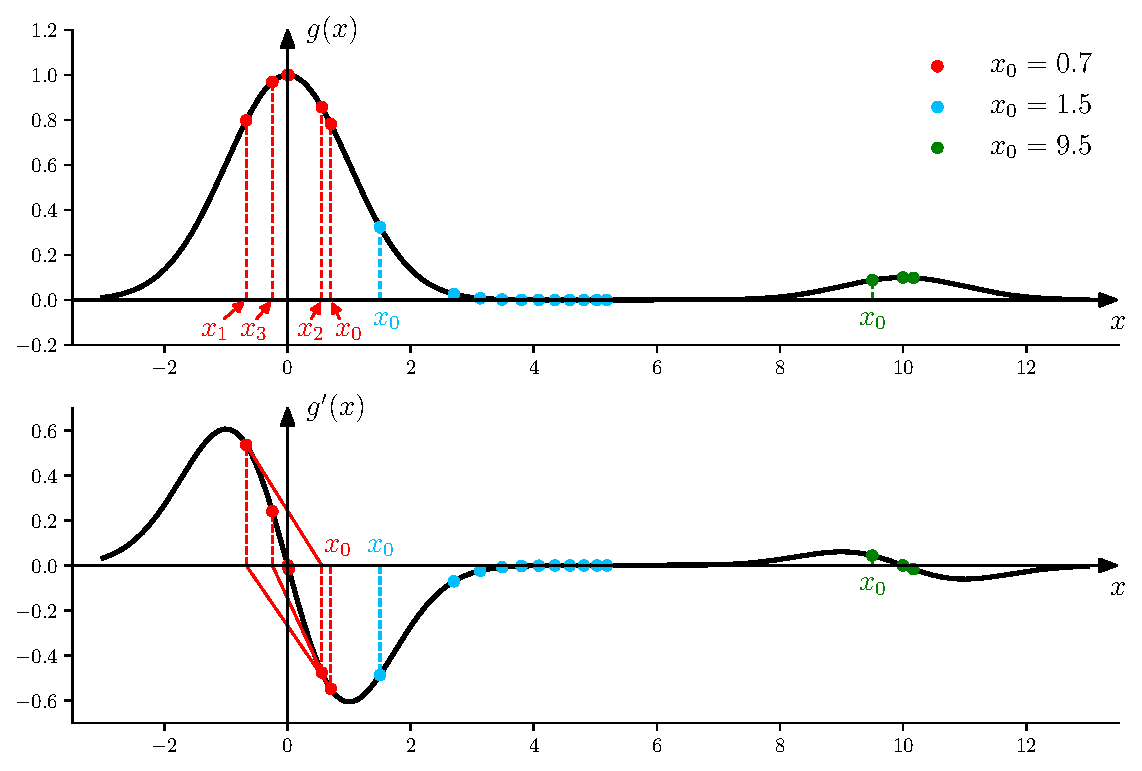
\includegraphics[width=0.9\textwidth]{figuras/problem_7_18.pdf}
\caption{\label{fig:problem_7_18} Método de Newton-Raphson para encontrar el máximo global de \(g(x)\). Se muestran las primeras 10 iteraciones para encontrar los ceros de \(g'(x)\) empleando distintos valores iniciales.}
\end{center}
\end{figure}
En la figura \ref{fig:problem_7_18} se muestran los resultados, específicamente, las 10 primeras iteraciones del método de Newton-Raphson. Se observa que en el caso en que \(x_0=0.7\), el algoritmo converge al máximo global de \(g(x)\) en \(x=0\), mientras que en el caso en que \(x_0=9.5\), la convergencia es al máximo local en \(x=10\). Cuando el valor inicial es \(x_0=1.5\), la convergencia es al mínimo en \(x\approx5.24\). Se concluye que para encontrar el máximo global, el valor inicial \(x_0\) del método de Newton-Raphson debe ser cercano al valor del máximo \(x_0=0\). 

\subsection{Problema 19}\label{sec:problem_7_19}

Si
\[
 x[n]=\cos2\pi f_0n+w[n],\qquad n=0,\,\dots,\,N-1
\]
donde \(w[n]\) es WGN de varianza \(\sigma^2\) conocida, mostrar que el MLE de la frecuencia se obtiene aproximadamente maximizando (\(f_0\) no cercano a 0 o 1/2)
\[
 \sum_{n=0}^{N-1}x[n]\cos2\pi f_0n
\]
sobre el intervalo \(0<f_0<1/2\). Luego, realizar una simulación Monte Carlo por computadora con \(N=10\), \(f_0=0.25\), \(\sigma^2=0.01\) y graficar la función a maximizar. Aplicar el algoritmo de Newton-Raphson para determinar el máximo y comparar los resultados con el obtenido mediante una búsqueda de grilla.

\paragraph{Solución} La PDF de los datos es 
\[
 p(\x;\,f_0)=\frac{1}{(2\pi\sigma^2)^\frac{N}{2}}\exp\left[-\frac{1}{2\sigma^2}\sum_{n=0}^{N-1}(x[n]-\cos2\pi f_0n)^2\right],
\]
por lo que la función de verosimilitud se maximiza al minimizar
\begin{align*}
 \tilde{J}(f_0)&=\sum_{n=0}^{N-1}(x[n]-\cos2\pi f_0n)^2\\
  &=\sum_{n=0}^{N-1}x^2[n]-2\sum_{n=0}^{N-1}x[n]\cos2\pi f_0n+\sum_{n=0}^{N-1}\cos^22\pi f_0n\\
  &\overset{(a)}{\approx}\sum_{n=0}^{N-1}x^2[n]-2\sum_{n=0}^{N-1}x[n]\cos2\pi f_0n+\frac{N}{2},
\end{align*}
donde en \((a)\) se tuvo en cuenta que la última sumatoria se puede aproximar como
\[
 \sum_{n=0}^{N-1}\cos^22\pi f_0n=\sum_{n=0}^{N-1}\frac{1+\cos4\pi f_0n}{2}\approx\frac{N}{2}
\]
empleando la aproximación demostrada en el problema \ref{sec:problem_3_7}. Además, como \(\tilde{J}(f_0)\) se minimiza maximizando el segundo sumando, el MLE se obtiene maximizando
\[
 J(f_0)=\sum_{n=0}^{N-1}x[n]\cos2\pi f_0n
\]
en \(0<f_0<1/2\), que es lo que se quería demostrar. En la gráfica de la figura \ref{fig:problem_7_19_J} se muestran 10 realizaciones de la función \(J(f_0)\) obtenidas mediante una simulación por computadora empleando los valores \(N=10\), \(f_0=0.25\) y \(\sigma^2=0.01\). Se observa que efectivamente el máximo se encuentra en todos los casos cercano al valor verdadero \(f_0=0.25\) del parámetro.
\begin{figure}[!htb]
\begin{center}
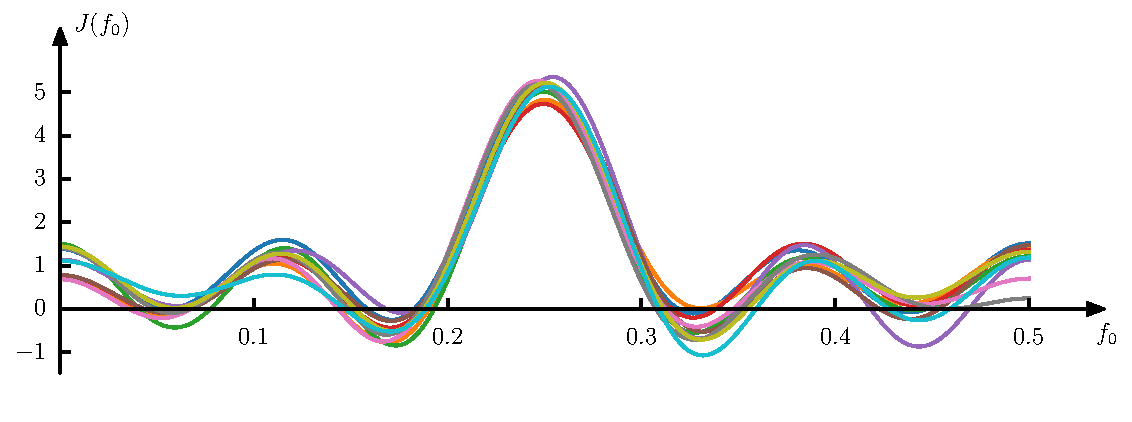
\includegraphics[width=0.9\textwidth]{figuras/problem_7_19_J.pdf}
\caption{\label{fig:problem_7_19_J} Función \(J(f_0)\) a maximizar para obtener el MLE de \(f_0\). El valor verdadero del parámetro a estimar es \(f_0=0.25\).}
\end{center}
\end{figure}

Se realizó la búsqueda del máximo en \(M=500\) realizaciones empleando una búsqueda de qrilla y el método de Newton-Raphson con distintos valores iniciales. En este caso, la estimación en el paso \(k\)-ésimo del método de Newton-Raphson es
\[
 {f_0}_{k+1}={f_0}_k-\frac{g(f_0)}{g'(f_0)},
\]
con
\[
 g(f_0)=J'(f_0)=-2\pi\sum_{n=0}^{N-1}nx[n]\sin2\pi f_0n,\qquad\qquad
 g'(f_0)=J''(f_0)=-(2\pi)^2\sum_{n=0}^{N-1}n^2x[n]\cos2\pi f_0n.
\]
En la siguiente tabla se muestran los resultados.
\begin{center}
\begin{tabular}{m{1.5cm}|>{\centering}m{1.5cm}|>{\centering}m{1.5cm}|>{\centering}m{1.5cm}|>{\centering}m{1.5cm}|m{1.5cm}<{\centering}|}
\cline{2-6}
 & \multirow{3}{*}{\begin{tabular}[c]{@{}c@{}}Búsqueda\\de\\grilla\end{tabular}} & \multicolumn{4}{c|}{Newton-Raphson} \\ \cline{3-6} 
                       &                       & \multicolumn{4}{c|}{valor inicial (\(f_{0_0}\))} \\ \cline{3-6} 
                       &                       & 0.22 & 0.23 & 0.26 & 0.28 \\ \hline
\multicolumn{1}{|c|}{\(E(\hat{f}_0)\)} & \multicolumn{1}{c|}{0.2500902} & 0.3233025 & 0.2500887 & 0.2500887 & 0.17483975 \\ \hline
\multicolumn{1}{|c|}{\(\var(\hat{f}_0)\)} & \multicolumn{1}{c|}{\(2.7\times10^{-6}\)} & \(1.3\times10^{-1}\) & \(2.6\times10^{-6}\) & \(2.6\times10^{-6}\) & \(5.0\times10^{0}\) \\ \hline
\end{tabular}
\end{center}
Se observa que con los valores iniciales (\(f_{0_0}=0.23\) y \(f_{0_0}=0.26\)), el método de Newton-Raphson converge al máximo global en las 500 realizaciones. Con los valores iniciales (\(f_{0_0}=0.23\) y \(f_{0_0}=0.26\)) el método no siempre converge al máximo global. En particular, con (\(f_{0_0}=0.23\) el método converge al mínimo ubicado en aproximadamente \(f_0=0.32\) en la mayoría de la realizaciones y con (\(f_{0_0}=0.28\) converge al mínimo en \(f_0=0.17\) en la mayoría de las realizaciones. En ambos casos, la varianza es grande debido a que en el resto de las realizaciones converge a un extremo arbitrario. En la figura \ref{fig:problem_7_19_estimations_v2} se muestra la estimación en las 500 realizaciones para todos los casos. Se observa que el método de Newton-Raphson converge al máximo global si el valor inicial es cercano al valor verdadero, que es el obtenido con la búsqueda de grilla.
\begin{figure}[!htb]
\begin{center}
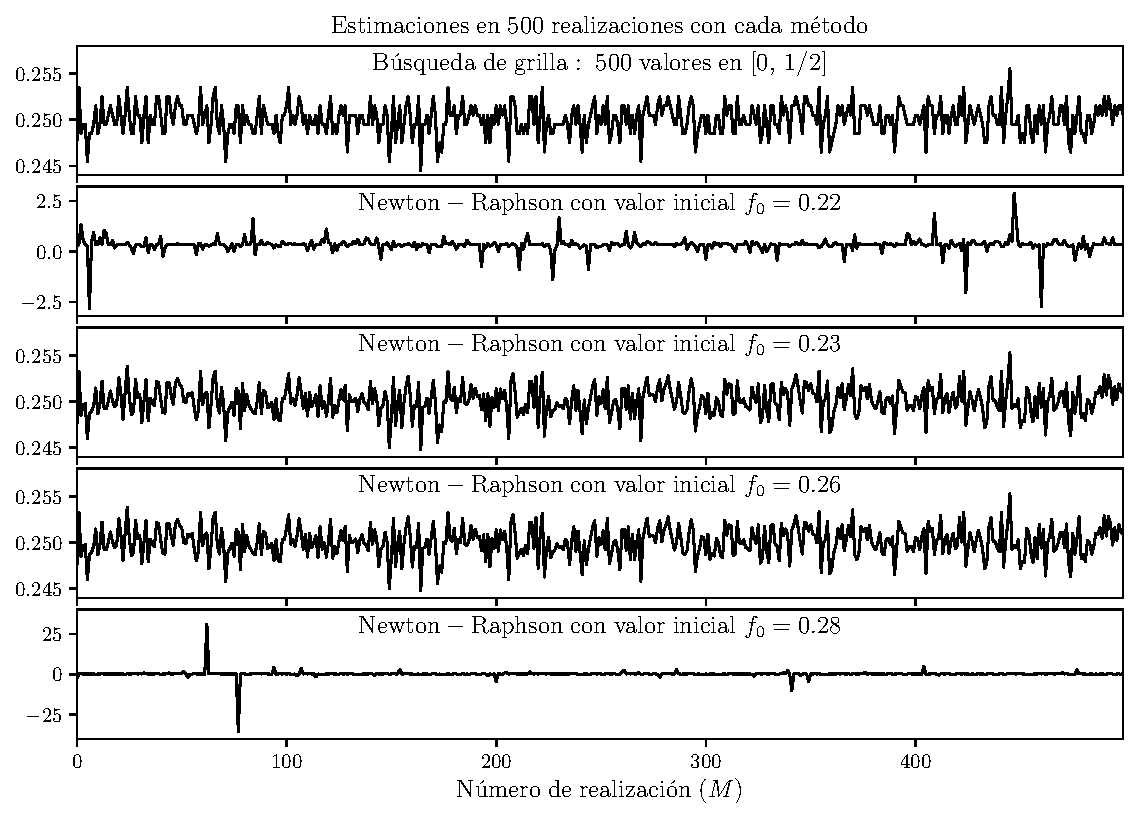
\includegraphics[width=\textwidth]{figuras/problem_7_19_estimations_v2.pdf}
\caption{\label{fig:problem_7_19_estimations_v2} Estimaciones del MLE de \(f_0\) en 500 realizaciones empleando búsqueda de grilla y el método de Newton-Raphson con distintos valores iniciales. El valor verdadero del parámetro a estimar es \(f_0=0.25\). Para la búsqueda en grilla se emplearon 500 valores de \(f_0\) en el intervalo \([0,\,1/2]\).}
\end{center}
\end{figure}

\subsection{Problema 20}

Se considera el conjunto de datos
\[
 x[n]=s[n]+w[n],\qquad n=0,\,\dots,\,N-1,
\]
donde \(s[n]\) es desconocido para \(n=0,\,\dots,\,N-1\) y \(w[n]\) es WGN de varianza conocida \(\sigma^2\). Determinar el MLE de \(s[n]\) y su PDF. ¿Se cumplen las propiedades asintóticas del MLE? Es decir, ¿es el MLE insesgado, eficiente, gaussiano y consistente?

\paragraph{Solución} La PDF de los datos es
\[
 p(\x;\,\s)=\frac{1}{(2\pi\sigma^2)^\frac{N}{2}}\exp\left[-\frac{1}{2\sigma^2}\sum_{n=0}^{N-1}(x[n]-s[n])^2\right],
\]
por lo que el MLE se obtiene minimizando
\[
 J(\s)=\sum_{n=0}^{N-1}(x[n]-s[n])^2.
\]
Derivando respecto al parámetro, se obtiene que
\[
 \frac{\partial J(\s)}{\partial s[k]}=-2(x[k]-s[k]),\qquad k=0,\,\dots,\,N-1
\]
e igualando a cero, se concluye que el MLE es
\[
 \hat{s}[k]=x[k],\qquad k=0,\,\dots,\,N-1,
\]
es decir
\[
 \hat{\s}=\x.
\]
Claramente, el MLE es insesgado, ya que
\[
 E(\hat{\s})=E(\x)=\s.
\]
Además, la matriz de covarianza del MLE es
\[
 \C_{\hat{\s}}=E[(\hat{\s}-\s)(\hat{\s}-\s)^T]=E(\w\w^T)=\sigma^2\I.
\]
Se concluye que el MLE es gaussiano con 
\[
 \hat{\s}\sim\mathcal{N}(\s,\,\sigma^2\I).
\]
Par ver si es eficiente, hay que calcular la CRLB. La función de verosimilitud logarítmica es
\[
 \ln p(\x;\,\s)=-\frac{N}{2}\ln2\pi\sigma^2 -\frac{1}{2\sigma^2}\sum_{n=0}^{N-1}(x[n]-s[n])^2.
\]
Diferenciando,
\[
 \frac{\partial\ln p(\x;\,\s)}{\partial s[k]}=\frac{1}{\sigma^2}(x[k]-s[k]),
\]
y diferenciando nuevamente
\[
 \frac{\partial^2\ln p(\x;\,\s)}{\partial s[k]\partial s[l]}=
 \left\{
 \begin{array}{cc}
  -\dfrac{1}{\sigma^2}, & k=l\\
  0& k\neq l
 \end{array}\right.
 =-\frac{1}{\sigma^2}\delta[k-l],
\]
resultando que la matriz de información de Fisher es
\[
 \I(\s)=\frac{1}{\sigma^2}\I,
\]
y la CRLB es
\[
 \var(\hat{s}[k])\geq[\I^{-1}(\s)]_{kk}=\sigma^2.
\]
Como el MLE alcanza la CRLB, es eficiente. Además, como 
\[
 \lim_{N\to\infty}\var(\hat{s}[k])=\sigma^2\neq0,
\]
el MLE no es consistente.

\subsection{Problema 21}

Para \(N\) observaciones IID con PDF \(\mathcal{N}(A,\,\sigma^2)\), donde \(A\) y \(\sigma^2\) son ambos desconocidos, encontrar el MLE de la SNR \(\alpha=A^2/\sigma^2\).

\paragraph{Solución} Por la propiedad de invarianza del MLE el MLE de \(\alpha\) es \(\hat{\alpha}=\hat{A}^2/\hat{\sigma^2}\), donde \(\hat{A}\) y \(\hat{\sigma^2}\) son los MLE de \(A\) y \(\sigma^2\) respectivamente. Para encontrar el MLE de \(\thetabf=[A\;\sigma^2]^T\) se parte de la PDF de los datos, que es
\[
 p(\x;\,\thetabf)=\frac{1}{(2\pi\sigma^2)^\frac{N}{2}}\exp\left[-\frac{1}{2\sigma^2}\sum_{n=0}^{N-1}(x[n]-A)^2\right].
\]
Del ejemplo de la sección \ref{sec:crlb_dc_in_wgn_dc_and_variance} se tiene que las derivadas de la función de verosimilitud logarítmica son
\[
 \frac{\partial\ln p(\x;\,\thetabf)}{\partial A}=\frac{1}{\sigma^2}\sum_{n=0}^{N-1}(x[n]-A)
 \qquad\qquad
 \frac{\partial\ln p(\x;\,\thetabf)}{\partial\sigma^2}=-\frac{N}{2\sigma^2}+\frac{1}{2\sigma^4}\sum_{n=0}^{N-1}(x[n]-A)^2
\]
Igualando a cero y despejando \(A\) en la primer ecuación se obtiene que
\[
 \hat{A}=\frac{1}{N}\sum_{n=0}^{N-1}x[n]=\bar{x}.
\]
Resolviendo para \(\sigma^2\) en la segunda ecuación y empleando el resultado anterior, se obtiene que
\[
 \frac{1}{\hat{\sigma^2}}\sum_{n=0}^{N-1}(x[n]-\bar{x})^2=N\qquad\qquad\Rightarrow\qquad\qquad
 \hat{\sigma^2}=\frac{1}{N}\sum_{n=0}^{N-1}(x[n]-\bar{x})^2.
\]
Se concluye que el MLE de \(\thetabf\) es
\[
 \hat{\thetabf}=
 \begin{bmatrix}
  \bar{x}\\
  \displaystyle\frac{1}{N}\sum_{n=0}^{N-1}(x[n]-\bar{x})^2
 \end{bmatrix}.
\]
Finalmente el MLE de \(\alpha\) es
\[
 \hat{\alpha}=\frac{\hat{A}^2}{\hat{\sigma^2}}=\frac{\bar{x}^2}{\displaystyle\frac{1}{N}\sum_{n=0}^{N-1}(x[n]-\bar{x})^2}.
\]

\subsection{Problema 22}\label{sec:problem_7_22}

Probar que si
\[
 \mathcal{A}(z)=1+\sum_{k=0}^{p}a[k]z^{-k}
\]
es un polinomio de fase mínima (todas las raíces se encuentran dentro del círculo unidad), se cumple que
\[
 \int_{-\frac{1}{2}}^{\frac{1}{2}}\ln|A(f)|^2\,df=0.
\]
Para hacerlo, probar primero que 
\[
 \int_{-\frac{1}{2}}^{\frac{1}{2}}\ln|A(f)|^2\,df=2\operatorname{Re}\left\{\frac{1}{2\pi j}\oint_C\ln\mathcal{A}(z)\,\frac{dz}{z}\right\},
\]
donde el contorno \(C\) es la circunferencia unidad en el plano \(z\). Luego, notar que 
\[
 \frac{1}{2\pi j}\oint_C\ln\mathcal{A}(z)\,\frac{dz}{z}
\]
es la transformada \(z\) inversa de \(\ln\mathcal{A}(z)\) evaluada en \(n=0\). Finalmente, emplear el hecho de que un polinomio \(\mathcal{A}(z)\) de fase mínima conduce a una transformada \(z\) inversa de \(\ln\mathcal{A}(z)\) que es una secuencia causal.

\paragraph{Solución} Esta propiedad se probó en la deducción de la CRLB asintótica para procesos WSS gaussianos de la sección \ref{sec:crlb_general_gaussian_wss} y por lo tanto, se incluye a continuación solo un esbozo de la demostración. En la ecuación \ref{eq:crlb_asymptotic_gaussian_fourier_z} se deduce que
\[
 \int_{-\frac{1}{2}}^{\frac{1}{2}}\ln|A(f)|^2 \,df=2\operatorname{Re}\left[\mathcal{Z}^{-1}\{\ln\mathcal{A}(z)\}\big|_{n=0}\right].
\]
Teniendo en cuenta que \(\mathcal{A}(z)\) es de fase mínima, todos los polos de \(\ln\mathcal{A}(z)\), que son los ceros de \(\mathcal{A}(z)\), se encuentran dentro del círculo unidad. Por lo tanto, la región de convergencia de \(\ln\mathcal{A}(z)\) es causal y contiene a la circunferencia unidad, resultando en una transformada \(z\) inversa causal y estable.
El teorema del valor inicial de la transformada \(z\) indica que para una secuencia \(x[n]\) que es nula en \(n<0\), es decir, que es causal, se cumple que
\[
 \lim_{z\to\infty}X(z)=x[0].
\]
Por lo tanto,
\begin{align*}
 \mathcal{Z}^{-1}\{\ln\mathcal{A}(z)\}\big|_{n=0}&=\lim_{z\to\infty}\ln\mathcal{A}(z)\\
   &=\ln\lim_{z\to\infty}\mathcal{A}(z)\\
   &=\ln a[0]\\
   &=\ln 1\\
   &=0,
\end{align*}
concluyendo que
\[
 \int_{-\frac{1}{2}}^{\frac{1}{2}}\ln|\mathcal{A}(z)|^2 \,df=0.
\]

\subsection{Problema 23}

Encontrar el MLE asintótico de la potencia total \(P_0\) de la PSD 
\[
 P_{xx}(f)=P_0Q(f)
\]
donde 
\[
 \int_{-\frac{1}{2}}^\frac{1}{2}Q(f)\,df=1.
\]
Si \(Q(f)=1\) para todo \(f\) tratándose de un proceso WGN, simplificar los resultados. Sugerencia: emplear los resultados del problema de la sección \ref{sec:problem_7_25} para la segunda parte.

\paragraph{Solución} EL MLE asintótico para un proceso gaussiano fue deducido en la sección \ref{sec:mle_asymptotic_gaussian} y cumple la condición (ecuación \ref{eq:mle_asymptotic_gaussian_mle_condition}) 
\[ 
 \int_{-\frac{1}{2}}^{\frac{1}{2}}\left[\frac{1}{P_{xx}(f)}-\frac{I(f)}{P_{xx}^2(f)}\right]\frac{\partial P_{xx}(f)}{\partial\theta_i}\,df=0,
\]
donde
\[
 I(f)=\frac{1}{N}\left|\sum_{n=0}^{N-1}x[n]e^{-j2\pi fn}\right|^2
\]
es el periodograma. Sustituyendo \(P_{xx}(f)\) y considerando que el parámetro a estimar es \(P_0\), se tiene que
\[
 \int_{-\frac{1}{2}}^{\frac{1}{2}}\left[\frac{1}{\hat{P}_0Q(f)}-\frac{I(f)}{\hat{P}_0^2Q^2(f)}\right]Q(f)\,df=
 \int_{-\frac{1}{2}}^{\frac{1}{2}}\left[\frac{1}{\hat{P}_0}-\frac{I(f)}{\hat{P}_0^2Q(f)}\right]\,df
 =\frac{1}{\hat{P}_0}-\frac{1}{\hat{P}_0^2}\int_{\frac{1}{2}}^{\frac{1}{2}}\frac{I(f)}{Q(f)}\,df=0,
\]
concluyendo que el MLE es
\[
 \hat{P}_0=\int_{\frac{1}{2}}^{\frac{1}{2}}\frac{I(f)}{Q(f)}\,df.
\]
En el caso en que \(Q(f)=1\) para todo \(f\), el MLE queda
\begin{align*}
 \hat{P}_0&=\int_{\frac{1}{2}}^{\frac{1}{2}}I(f)\,df\\
  &\overset{(a)}{=}\frac{1}{N}\int_{\frac{1}{2}}^{\frac{1}{2}}X'(f)X'^*(f)\,df\\
  &=\frac{1}{N}\int_{\frac{1}{2}}^{\frac{1}{2}}|X'(f)|^2\,df\\
  &=\frac{1}{N}\sum_{n=-\infty}^{-\infty}x'^2[n]
\end{align*}
donde en \((a)\) se consideró que \(I(f)=X'(f){X'}^*(f)/N\) como se muestra en el problema de la sección \ref{sec:problem_7_25} y en \((b)\) se empleó la identidad de Parseval. Considerando la definicón de \(x'[n]\) en el problema \ref{sec:problem_7_25}, se concluye que 
\[
 \hat{P}_0=\frac{1}{N}\sum_{n=0}^{N-1}x^2[n].
\]

\subsection{Problema 24}

En el ejemplo de la sección \ref{sec:mle_sinusoidal_parameters} se mostró que el pico del periodograma es el MLE de la frecuencia con la condición de que \(f_0\) no esté cerca de 0 o 1/2. Graficar el periodograma para \(N=10\) para las frecuencias \(f_0=0.25\) y \(f_0=0.05\) de los datos no ruidosos
\[
 x[n]=\cos2\pi f_0n,\qquad n=0,\,\dots,\,N-1.
\]
¿Qué ocurre si la aproximación no es válida? Repetir el problema empleando la función exacta
\[
 J(f)=\x^T\Hbf(\Hbf^T\Hbf)^{-1}\Hbf^T\x
\]
donde \(\Hbf\) está definido en el ejemplo de la sección \ref{sec:mle_sinusoidal_parameters}.

\paragraph{Solución} En el ejemplo de la sección \ref{sec:mle_sinusoidal_parameters} se mostró que el MLE de \(f_0\) se obtiene maximizando la función
\[
 J(f)=\x^T\Hbf(\Hbf^T\Hbf)^{-1}\Hbf^T\x,
\]
donde \(\Hbf=[\mathbf{c}\,\s]\) es una matriz \(N\times2\) con
\[
 \mathbf{c}=[1\;\cos2\pi f\,\dots\,\cos2\pi f(N-1)]^T
 \qquad\textrm{y}\qquad
 \s=[0\;\sin2\pi f\,\dots\,\sin2\pi f(N-1)]^T.
\]
Además, empleando aproximaciones como la deducida en el ejercicio \ref{sec:problem_3_7}, se mostró que para \(f_0\) no cercano a 0 o 1/2, la función a maximizar se puede aproximar por el periodograma, es decir,
\[
 J(f)\approx I(f)=\frac{2}{N}\left|\sum_{n=0}^{N-1}x[n]e^{-j2\pi fn}\right|^2.
\]
En la figura \ref{fig:problem_7_24} se muestra la función \(J(f)\) exacta y aproximada cuando  \(f_0=0.25\) y \(f_0=0.05\).
\begin{figure}[!htb]
\begin{center}
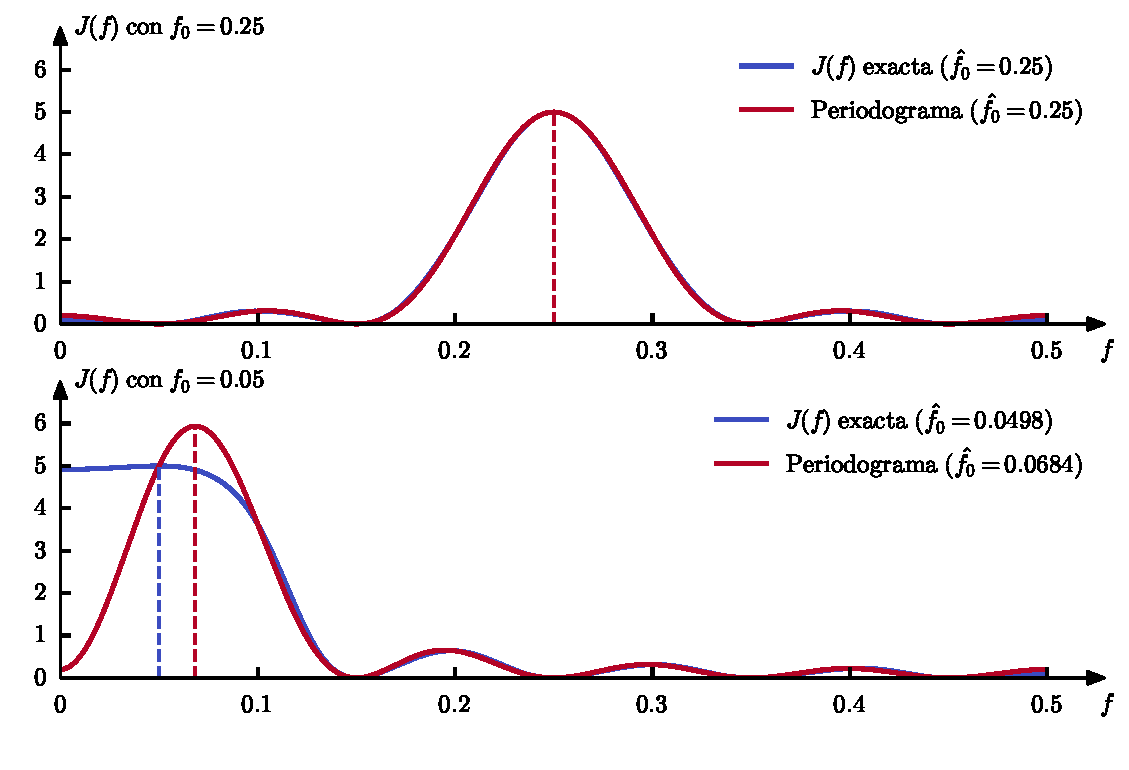
\includegraphics[width=\textwidth]{figuras/problem_7_24.pdf}
\caption{\label{fig:problem_7_24} MLE de \(f_0\). Se muestra la función a maximizar \(J(f)\) exacta y la aproximación por el periodograma \(I(f)\) para los valores verdaderos \(f_0=0.25\) y \(f_0=0.05\). Se indica el máximo de la función en cada caso.}
\end{center}
\end{figure}
Se observa que para \(f_0=0.25\) el periodograma es una buena aproximación de \(J(f)\) y por lo tanto, el estimador MLE es bueno. Cuando \(f_0=0.05\), que es cercano a 0, no se cumple la aproximación deducida en el ejercicio \ref{sec:problem_3_7} y por lo tanto, no se cumple que \(J(f)\approx I(f)\). En ese caso, el pico del periodograma está desplazado del valor verdadero. Esto se debe al solapamiento de los picos producidos por las sinusoides en \(f_0=0.05\) y \(f_0=-0.05\), que no son bien resueltas en el periodograma debido a que el número de muestras \(N=10\) es pequeño.


\subsection{Problema 25}\label{sec:problem_7_25}

Probar que la transformada inversa de Fourier del periodograma es
\[
\def\arraystretch{1.4}
 \hat{r}_{xx}[k]=
 \left\{\begin{array}{ll}
   \displaystyle\frac{1}{N}\sum_{n=0}^{N-1-|k|}x[n]x[n+|k|] &  |k|\leq N-1\\
   0 &  |k|\geq N.
 \end{array}\right.
\]
Sugerencia: notar que el periodograma puede escribirse como
\[
 I(f)=\frac{1}{N}X'(f){X'}^*(f),
\]
donde \(X'(f)\) es la transformada de Fourier de la secuencia
\[
 x'[n]=
 \left\{\begin{array}{ll}
   x[n] &  0 \leq n \leq N-1\\
   0 &  \textrm{ en otro caso}.
 \end{array}\right.
\]

\paragraph{Solución} Por definición, el periodograma es
\begin{align*}
 I(f)&=\frac{1}{N}\left|\sum_{n=0}^{N-1}x[n]e^{-j2\pi fn}\right|^2\\
  &=\frac{1}{N}\left|\sum_{n=-\infty}^{\infty}x'[n]e^{-j2\pi fn}\right|^2\\
  &=\frac{1}{N}X'(f){X'}^*(f),
\end{align*}
donde \(X'(f)\) es la transformada de Fourier de \(x'[n]\), es decir,
\[
 x'[n]\overset{\mathcal{F}}{\longleftrightarrow}X'(f)=\sum_{n=-\infty}^{\infty}x'[n]e^{-j2\pi fn}.
\]
\(I(f)\) puede escribirse como
\begin{align*}
 I(f)&=\frac{1}{N}\left(\sum_{m=-\infty}^{\infty}x'[m]e^{-j2\pi fm}\right)\left(\sum_{n=-\infty}^{\infty}x'[n]e^{-j2\pi fn}\right)^*\\
  &\overset{(a)}{=}\frac{1}{N}\left(\sum_{m=-\infty}^{\infty}x'[m]e^{-j2\pi fm}\right)\left(\sum_{n=-\infty}^{\infty}x'[n]e^{j2\pi fn}\right)\\
  &=\frac{1}{N}\sum_{m=-\infty}^{\infty}\sum_{n=-\infty}^{\infty}x'[m]x'[n]e^{-j2\pi f(m-n)}\\
  &\overset{(b)}{=}\frac{1}{N}\sum_{l=-\infty}^{\infty}\sum_{n=-\infty}^{\infty}x'[n+l]x'[n]e^{-j2\pi fl},
\end{align*}
donde en \((a)\) se consideró que \(x'[n]\) es real y en \((b)\) se realizó el cambio de variable \(l=m-n\). Aplicando la transformada de Fourier inversa se tiene que
\begin{align*}
 \mathcal{F}^{-1}\{I(f)\}&=\int_{-\frac{1}{2}}^\frac{1}{2}\frac{1}{N}\sum_{l=-\infty}^{\infty}\sum_{n=-\infty}^{\infty}x'[n+l]x'[n]e^{-j2\pi fl}e^{j2\pi fk}\,df\\
  &=\frac{1}{N}\sum_{l=-\infty}^{\infty}\sum_{n=-\infty}^{\infty}x'[n+l]x'[n]\int_{-\frac{1}{2}}^\frac{1}{2}e^{j2\pi f(k-l)}\,df
\end{align*}
Ahora,
\begin{align*}
 \int_{-\frac{1}{2}}^\frac{1}{2}e^{j2\pi f(k-l)}\,df&=\frac{e^{j2\pi f(k-l)}}{j2\pi (k-l)}\bigg|_{-\frac{1}{2}}^{\frac{1}{2}}\\
  &=\frac{e^{j\pi(k-l)}+e^{-j\pi(k-l)}}{j2\pi(k-l)}\\
  &=\frac{\sin\pi(k-l)}{\pi(k-l)}\\
  &\overset{(a)}{=}\delta[k-l].
\end{align*}
donde en \((a)\) se empleó la regla de L'Hôpital para evaluar \(\sin\pi x/\pi x\) en \(x=0\),
\[
 \lim _{x\to 0}\frac{\sin\pi x}{\pi x}=\lim _{x\to 0}\frac{\pi\cos\pi x}{\pi}=1.
\]
Por lo tanto, la transformada inversa de Fourier del periodograma queda
\begin{align*}
 \mathcal{F}^{-1}\{I(f)\}&=\frac{1}{N}\sum_{l=-\infty}^{\infty}\sum_{n=-\infty}^{\infty}x'[n+l]x'[n]\delta[k-l]\\
  &=\frac{1}{N}\sum_{n=-\infty}^{\infty}x'[n+k]x'[n].
\end{align*}
Considerando que 
\[
\def\arraystretch{1.4}
 \begin{array}{ccc}
  x'[n]=x[n]\neq0 & \textrm{en} & n=[0,\,N-1]\\
  x'[n+k]=x[n+k]\neq0 & \textrm{en} & n=[-k,\,N-1-k]
 \end{array},
\]
para \(0\leq k\leq N-1\) se tiene que
\[
 \mathcal{F}^{-1}\{I(f)\}=\frac{1}{N}\sum_{n=0}^{N-1-k}x[n+k]x[n]
\]
y para \(-(N-1)\leq k<0\),
\begin{align*}
 \mathcal{F}^{-1}\{I(f)\}&=\frac{1}{N}\sum_{n=-k}^{N-1}x[n+k]x[n]\\
  &\overset{(a)}{=}\frac{1}{N}\sum_{m=0}^{N-1+k}x[m]x[m-k]\\
  &\overset{(b)}{=}\frac{1}{N}\sum_{m=0}^{N-1-|k|}x[m]x[m+|k|]
\end{align*}
donde en \((a)\) se realizó el cambio de variable \(m=n+k\) y en \((b)\) se tuvo en cuenta que como \(k<0\), \(k=-|k|\). Combinando los resultados, se concluye que
\[
\def\arraystretch{1.4}
 \mathcal{F}^{-1}\{I(f)\}=\hat{r}_{xx}[k]=
 \left\{\begin{array}{ll}
   \displaystyle\frac{1}{N}\sum_{n=0}^{N-1-|k|}x[n]x[n+|k|] &  |k|\leq N-1\\
   0 &  |k|\geq N,
 \end{array}\right.
\]
que es lo que se quería demostrar.

El resultado puede obtenerse de forma mas directa empleando propiedades de la transformada de Fourier. Como
\[
  I(f)=\frac{1}{N}X'(f){X'}^*(f),
\]
considerando que
\[
 x[n]\overset{\mathcal{F}}{\longleftrightarrow}X(f)\qquad\qquad\Rightarrow\qquad\qquad
 x[-n]\overset{\mathcal{F}}{\longleftrightarrow}X^*(f)
\]
y que
\[
 \begin{array}{c}
  x[n]\overset{\mathcal{F}}{\longleftrightarrow}X(f)\\
  y[n]\overset{\mathcal{F}}{\longleftrightarrow}Y(f)
 \end{array}
 \qquad\qquad\Rightarrow\qquad\qquad
 x[n]*y[n]\overset{\mathcal{F}}{\longleftrightarrow}X(f)Y(f)
\]
se cumple que
\[
 x[n]*x[-n]\overset{\mathcal{F}}{\longleftrightarrow}X(f)X^*(f).
\]
Por lo tanto,
\[
 \mathcal{F}^{-1}\{I(f)\}=\frac{1}{N}x'[n]*x'[-n]=\frac{1}{N}\sum_{n=-\infty}^{\infty}x'[-n]x'[k-n]=\frac{1}{N}\sum_{m=-\infty}^{\infty}x'[m]x'[m+k].
\]

\subsection{Problema 26}

La PSD de un proceso AR(1) está dada por 
\[
 P_{xx}(f)=\frac{\sigma_u^2}{|1+a[1]e^{-j2\pi f}|^2}.
\]
Si \(a[1]\) y \(\sigma^2\) son desconocidos, encontrar el MLE de \(P_{xx}(f)\) para \(f=f_0\) empleando las ecuaciones \ref{eq:mle_ar_estimation_yule_walker1} y \ref{eq:mle_ar_estimation_yule_walker2}. ¿Cual es la varianza asintótica del MLE? Sugerencia: emplear las ecuaciones \ref{eq:crlb_vector_transformations} y \ref{eq:crlb_asymptotic_ar_process_fisher_matrix}.

\paragraph{Solución} Para calcular el MLE de \(P_{xx}(f_0)\), se calculará primero el MLE de \(a[1]\) y \(\sigma^2\). Luego, el MLE de \(P_{xx}(f_0)\) se obtiene inmediatamente gracias a la propiedad de invarianza ante transformaciones del MLE. De las ecuaciones \ref{eq:mle_ar_estimation_yule_walker1} y \ref{eq:mle_ar_estimation_yule_walker2} de Yule-Walker con \(p=1\) se tiene que
\[
\left\{
 \begin{array}{l}
  \hat{r}_{xx}[0]\hat{a}[1]=-\hat{r}_{xx}[1]\\
  \hat{\sigma^2_u}=r_{xx}[0]+\hat{a}[1]\hat{r}_{xx}[1]
 \end{array}\right.,
\]
donde \(\hat{r}_{xx}[k]\) es la ACF muestral de los datos \(x[n]\), que está dada por la ecuación \ref{eq:mle_ar_estimation_sample_acf}. Por lo tanto, de la primer ecuación se obtiene que 
\[
 \hat{a}[1]=-\frac{\hat{r}_{xx}[1]}{\hat{r}_{xx}[0]}
\]
y sustituyendo este resultado en la segunda ecuación, se obtiene que 
\[
 \hat{\sigma^2_u}=\hat{r}_{xx}[0]-\frac{\hat{r}_{xx}^2[1]}{\hat{r}_{xx}[0]}=\frac{\hat{r}_{xx}^2[0]-\hat{r}_{xx}^2[1]}{\hat{r}_{xx}[0]}.
\]
Finalmente, por la propiedad de invarianza, el MLE de \(P_{xx}(f_0)\) es
\[
 \hat{P}_{xx}(f_0)=\frac{\hat{\sigma_u^2}}{|1+\hat{a}[1]e^{-j2\pi f_0}|^2}.
\]

Para calcular la varianza asintótica del MLE, se considera que se cumple que el MLE es asintóticamente distribuido como
\[
 \hat{P}_{xx}(f_0)\overset{a}{\sim}\mathcal{N}(P_{xx}(f_0), \I^{-1}(P_{xx}(f_0))),
\]
como se explicó en la sección \ref{sec:mle_asintotic_properties}. Además, como \(P_{xx}(f_0)\) es una transformación del parámetro vectorial \(\thetabf=[a[1]\;\sigma^2_u]^T\), \(\I^{-1}(P_{xx}(f_0))\) está dado por la ecuación \ref{eq:crlb_vector_transformations},
\[
 \I^{-1}(P_{xx}(f_0))=\frac{\partial g(\thetabf)}{\partial\thetabf}\I^{-1}(\thetabf)\frac{\partial g(\thetabf)}{\partial\thetabf}^T.
\]
donde la matriz de información de Fisher \(\I(\thetabf)\) fue calculada en el ejemplo del cálculo del MLE de los parámetros de un proceso AR de la sección \ref{sec:ar_parameters_estimation} y está dada por la ecuación \ref{eq:crlb_asymptotic_ar_process_fisher_matrix}, que con \(p=1\) es
\[
 \I(\thetabf)=
 \begin{bmatrix}
    \displaystyle\frac{N}{\sigma_u^2}r_{xx}[0] & 0\\
    0 & \displaystyle\frac{N}{2\sigma_u^4}
 \end{bmatrix}
 \qquad\qquad\Rightarrow\qquad\qquad
 \I^{-1}(\thetabf)=
 \begin{bmatrix}
    \displaystyle\frac{\sigma_u^2}{Nr_{xx}[0]} & 0\\
    0 & \displaystyle\frac{2\sigma_u^4}{N}
 \end{bmatrix}.
\]
Además, la transformación \(g\) es en este caso
\[
 g(\thetabf)=\frac{\sigma_u^2}{|1+a[1]e^{-j2\pi f_0}|^2}=\frac{\sigma_u^2}{|A(f_0)|^2},
\]
donde se definió \(A(f_0)=1+a[1]e^{-j2\pi f_0}\). Considerando que
\[
 \frac{\partial g(\thetabf)}{\partial\thetabf}=
 \begin{bmatrix}
  \dfrac{\partial g(\thetabf)}{\partial a[1]} & \dfrac{\partial g(\thetabf)}{\partial\sigma_u^2}
 \end{bmatrix},
\]
se tiene que
\begin{align*}
 \frac{\partial g(\thetabf)}{\partial a[1]}&=-\frac{\sigma_u^2}{|A(f_0)|^4}\frac{\partial |A(f_0)|^2}{\partial a[1]}\\
 &=-\frac{\sigma_u^2}{|A(f_0)|^4}\frac{\partial A(f_0)A^*(f_0)}{\partial a[1]}\\
 &=-\frac{\sigma_u^2}{|A(f_0)|^4}\left[A(f_0)\frac{\partial A^*(f_0)}{\partial a[1]}+A^*(f_0)\frac{\partial A(f_0)}{\partial a[1]}\right]\\
 &=-\frac{\sigma_u^2}{|A(f_0)|^4}\left[A(f_0)e^{j2\pi f_0}+A^*(f_0)e^{-j2\pi f_0}\right]\\
 &=-\frac{2\sigma_u^2}{|A(f_0)|^4}\operatorname{Re}\left\{A(f_0)e^{j2\pi f_0}\right\}
\end{align*}
y como
\[
 \operatorname{Re}\left\{A(f_0)e^{j2\pi f_0}\right\}=\operatorname{Re}\left\{(1+a[1]e^{-j2\pi f})e^{j2\pi f_0}\right\}=
 \operatorname{Re}\left\{(e^{j2\pi f_0}+a[1])\right\}=a[1]+\cos2\pi f_0,
\]
se obtiene que
\[
 \frac{\partial g(\thetabf)}{\partial a[1]}=-\frac{2\sigma_u^2(a[1]+\cos2\pi f_0)}{|A(f)|^4}.
\]
Por otro lado,
\[
 \frac{\partial g(\thetabf)}{\partial\sigma_u^2}=\frac{1}{|A(f_0)|^2},
\]
concluyendo que
\[
 \frac{\partial g(\thetabf)}{\partial\thetabf}=
 \begin{bmatrix}
  -\dfrac{2\sigma_u^2(a[1]+\cos2\pi f_0)}{|A(f_0)|^4} & \dfrac{1}{|A(f_0)|^2}
 \end{bmatrix}.
\]
Luego,
\[
 \I^{-1}(\thetabf)\frac{\partial g(\thetabf)}{\partial\thetabf}^T=
 \begin{bmatrix}
    \displaystyle\frac{\sigma_u^2}{Nr_{xx}[0]} & 0\\
    0 & \displaystyle\frac{2\sigma_u^4}{N}
 \end{bmatrix}
 \def\arraystretch{2.4}
 \begin{bmatrix}
  -\dfrac{2\sigma_u^2(a[1]+\cos2\pi f_0)}{|A(f_0)|^4}\\
  \dfrac{1}{|A(f_0)|^2}
 \end{bmatrix}=
 \begin{bmatrix}
  -\dfrac{2\sigma_u^4(a[1]+\cos2\pi f_0)}{Nr_{xx}[0]|A(f_0)|^4}\\
  \dfrac{2\sigma_u^4}{N|A(f_0)|^2}
 \end{bmatrix},
\]
y
\begin{align*}
 \frac{\partial g(\thetabf)}{\partial\thetabf}\I^{-1}(\thetabf)\frac{\partial g(\thetabf)}{\partial\thetabf}^T&=
 \begin{bmatrix}
  -\dfrac{2\sigma_u^2(a[1]+\cos2\pi f_0)}{|A(f_0)|^4} & \dfrac{1}{|A(f_0)|^2}
 \end{bmatrix}
 \def\arraystretch{2.4}
 \begin{bmatrix}
  -\dfrac{2\sigma_u^4(a[1]+\cos2\pi f_0)}{Nr_{xx}[0]|A(f_0)|^4}\\
  \dfrac{2\sigma_u^4}{N|A(f_0)|^2}
 \end{bmatrix}\\
 &=\dfrac{4\sigma_u^6(a[1]+\cos2\pi f_0)^2}{Nr_{xx}[0]|A(f_0)|^8}+\dfrac{2\sigma_u^4}{N|A(f_0)|^4}.
\end{align*}
Se concluye que
\begin{equation}\label{eq:mle_ar1_estimation_asymp_variance}
  \I^{-1}(P_{xx}(f_0))=\frac{4P_{xx}^4(f_0)(a[1]+\cos2\pi f_0)^2}{N\sigma_u^2r_{xx}[0]}+\frac{2P_{xx}^2(f_0)}{N}
\end{equation}
es la varianza asintótica del MLE de \(P_{xx}(f_0)\).

Se realizó una simulación por computadora que consistió en generar \(N=40\) y \(N=400\) muestras del proceso AR(1) con parámetros \(a[1]=-0.9\) y \(\sigma_u^2=1\), y se calculó el MLE \(\hat{P}_{xx}(f)\) y su varianza \(\var(\hat{P}_{xx}(f))\). En la figura \ref{fig:problem_7_26} se muestran los resultados, en donde se grafica el promedio de \(M=10000\) realizaciones de \(\hat{P}_{xx}(f)\) y \(\var(\hat{P}_{xx}(f))\) junto con el valor verdadero de \(P_{xx}(f)\) y la varianza asintótica \(\operatorname{CRLB}(P_{xx}(f))\) dada por la ecuación \ref{eq:mle_ar1_estimation_asymp_variance}, en donde \(r_{xx}[0]\) se calcula como (ver el ejemplo de la sección \ref{sec:ar_parameters_estimation})
\[
 r_{xx}[0]=\frac{\sigma_u^2}{1-a^2[1]}.
\]
Como es de esperar, se observa que cuando el largo \(N\) de los datos es pequeño, la varizana del estimador difiere considerablemente de la varianza asintótica teórica, pero se acerca cada vez mas al incrementar \(N\). 
\begin{figure}[!htb]
\begin{center}
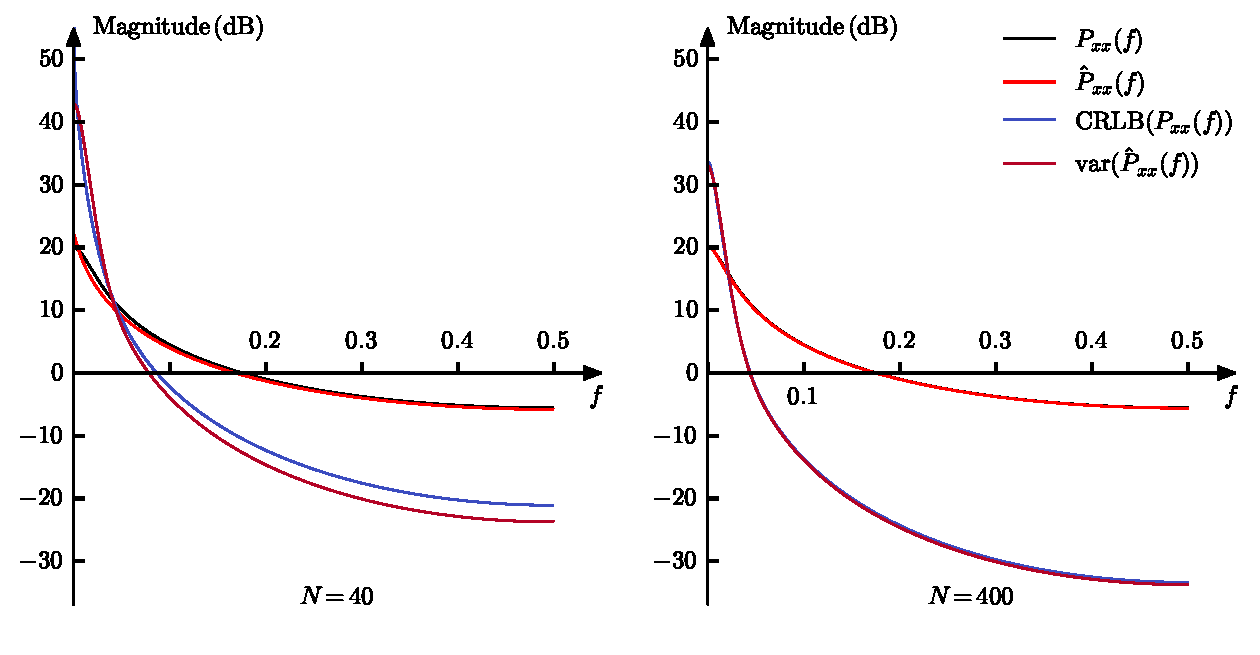
\includegraphics[width=\textwidth]{figuras/problem_7_26.pdf}
\caption{\label{fig:problem_7_26} Comparación de la varianza asintótica teórica del MLE de \(P_{xx}(f)\) con la varianza calculada en \(M=10000\) realizaciones empleando un largo de datos de \(N=40\) y \(N=400\) muestras.}
\end{center}
\end{figure}

\chapter{Mínimos cuadrados}

\section{Enfoque de mínimos cuadrados}

El enfoque empleado hasta ahora para considerar que un estimador es bueno, es que sea insesgado y tenga varianza mínima. Al elegir la varianza como medida de calidad, se busca minimizar la discrepancia entre el estimador y el valor verdadero del parámetro \emph{en promedio}. En el enfoque de mínimos cuadrados (\emph{least squares}, LS) se intenta minimizar la diferencia cuadrática entre los datos \(x[n]\) \emph{observados} y el modelo \(s[n]\) asumido de los datos. La señal \(s[n]\) es determinística y depende del parámetro \(\theta\) desconocido que se quiere estimar. La diferencia entre los datos observados \(x[n]\) y el modelo \(s[n]\) se debe a ruido de observación o inexactitudes de modelado.
El estimador de mínimos cuadrados (\emph{least squares estimator}, LSE) de \(\theta\) es aquel que minimiza el error cuadrático medio
\[
 J(\theta)=\sum_{n=0}^{N-1}(x[n]-s[n])^2.
\]
En este enfoque no se asume ninguna hipótesis sobre las propiedades estadísticas de los datos \(x[n]\). El LSE es generalemnte empleado en situaciones donde no se dispone de una caracterización estadísitca precisa de los datos, pero también cuando es difícil o no es posible encontrar un estimador óptimo. 

En el caso en que el modelo de señal es lineal con el parámetro a estimar, el error cuadrático es una función cuadrática con el parámetro, por lo que el mínimo se obtiene fácilmente y el problema de encontrar el LSE se denomina problema de mínimos cuadrados lineal.
En el caso no lineal, en general no es posible obtener una expresión analítica del mínimo, y deben emplearse métodos iterativos o búsqueda de grilla, y el problema se denomina mínimos cuadrados no lineal.

\section{Mínimos cuadrados lineales}

\subsection{Caso escalar}

Para aplicar el enfoque de LS lineal, se asume que el modelo de señal es
\[
 s[n]=\theta h[n],
\]
donde \(h[n]\) es una señal conocida. La función del error LS es
\begin{equation}\label{eq:ls_lls_criterion_scalar}
 J(\theta)=\sum_{n=0}^{N-1}(x[n]-\theta h[n])^2.
\end{equation}
El LSE se obtiene diferenciando respecto al parámetro e igualando a cero. La derivada respecto al parámetro es
\[
 \frac{\partial J(\theta)}{\partial \theta}=-2\sum_{n=0}^{N-1}(x[n]-\theta h[n])h[n],
\]
e igualando a cero y despejando el parámetro se obtiene que 
\begin{equation}\label{eq:ls_lls_estimator_scalar}
 \hat{\theta}=\frac{\displaystyle
 \sum_{n=0}^{N-1}x[n]h[n]}{\displaystyle\sum_{n=0}^{N-1}h^2[n]}.
\end{equation}
El error mínimo se obtiene sustituyendo la ecuación \ref{eq:ls_lls_estimator_scalar} en la \ref{eq:ls_lls_criterion_scalar} y es
\begin{align*}
 J_\textrm{mín}=J(\hat{\theta})&=\sum_{n=0}^{N-1}(x[n]-\hat{\theta}h[n])(x[n]-\hat{\theta}h[n])\\
   &=\sum_{n=0}^{N-1}x[n](x[n]-\hat{\theta}h[n])-\hat{\theta}\sum_{n=0}^{N-1}h[n](x[n]-\hat{\theta}h[n])\\
   &\overset{(a)}{=}\sum_{n=0}^{N-1}x^2[n]-\hat{\theta}\sum_{n=0}^{N-1}x[n]h[n],
\end{align*}
donde en \((a)\) se consideró que la segunda sumatoria es nula. Efectivamente,
\begin{align*}
 \sum_{n=0}^{N-1}h[n](x[n]-\hat{\theta}h[n])&\overset{(a)}{=}\sum_{n=0}^{N-1}h[n]\left(x[n]-\frac{\displaystyle
 \sum_{n=0}^{N-1}x[n]h[n]}{\displaystyle\sum_{n=0}^{N-1}h^2[n]}h[n]\right)\\
 &=\sum_{n=0}^{N-1}h[n]x[n]-\frac{\displaystyle
 \sum_{n=0}^{N-1}x[n]h[n]}{\displaystyle\sum_{n=0}^{N-1}h^2[n]}\sum_{n=0}^{N-1}h^2[n]\\
 &=0,
\end{align*}
donde en \((a)\) se sustituyó el LSE dado por la ecuación \ref{eq:ls_lls_estimator_scalar}. Sustituyendo nuevamente la ecuación \ref{eq:ls_lls_estimator_scalar} el error mínimo se puede escribir como
\begin{equation}\label{eq:ls_lls_min_error_scalar}
 J_\textrm{mín}=\sum_{n=0}^{N-1}x^2[n]-\frac{\left(\displaystyle
 \sum_{n=0}^{N-1}x[n]h[n]\right)^2}{\displaystyle\sum_{n=0}^{N-1}h^2[n]}.
\end{equation}
En el problema de la sección \ref{sec:problem_8_2} se muestra que se cumple que
\begin{equation}\label{eq:ls_lls_min_error_bounds}
  0\leq J_\textrm{mín} \leq\sum_{n=0}^{N-1}x^2[n].
\end{equation}

\subsection{Caso vectorial}

La extensión al caso en que el parámetro a estimar es un vector \(\thetabf\) de dimensiones \(p\times1\) es directa. El modelo de señal \(\s=[s[0]\,s[1]\dots s[N-1]]^T\) lineal con el parámetro es
\[
 \s=\Hbf\thetabf,
\]
donde \(\Hbf\) es una matriz conocida \(N\times p\) con \(N>p\), de rango completo \(p\), denominada \emph{matriz de observación}. El LSE se encuentra minimizando 
\[
 J(\thetabf)=\sum_{n=0}^{N-1}(x[n]-s[n])^2=(\x-\Hbf\thetabf)^T(\x-\Hbf\thetabf).
\]
Calculando el gradiente e igualando a cero se obtiene que el LSE es
\begin{equation}\label{eq:ls_lls_estimator_vector}
 \hat{\thetabf}=(\Hbf^T\Hbf)^{-1}\Hbf^T\x.
\end{equation}
 Las ecuaciones \(\Hbf^T\Hbf\hat{\thetabf}=\Hbf\x\) a resolver para calcular \(\hat{\thetabf}\) se llaman \emph{ecuaciones normales}. La hipótesis del rango completo de \(\Hbf\) asegura que \(\Hbf^T\Hbf\) es invertible. En el problema de la sección \ref{sec:problem_8_4} se deriva el resultado de una forma alternativa. Además, el error mínimo es
\begin{equation}\label{eq:ls_lls_min_error_vector}
  J_\textrm{mín}=J(\hat{\thetabf})=\x^T(\I-\Hbf(\Hbf^T\Hbf)^{-1}\Hbf^T)\x.
\end{equation}

\subsection{Interpretación geométrica}\label{sec:ls_lls_geometric_interpretation}

El modelo de la señal es
\[
 \s=\Hbf\thetabf=
 \begin{bmatrix}
  \h_1 & \h_2 & \dots & \h_p
 \end{bmatrix}
 \begin{bmatrix}
  \theta_1\\
  \theta_2\\
  \vdots\\
  \theta_p
 \end{bmatrix}
 =\sum_{i=1}^{p}\theta_i\h_i,
\]
donde \(\h_i\) son las columnas de la matriz \(\Hbf\). Esto indica que el modelo de señal es una combinación lineal de las columnas de \(\Hbf\). Definiendo el largo de un vector \(\bm{\xi}=[\xi_1\,\xi_2\,\dots\,\xi_N]^T\) como la norma euclideana,
\[
 \lVert\bm{\xi}\rVert=\sqrt{\sum_{i=1}^{N}\xi_i^2}=\sqrt{\bm{\xi}^T\bm{\xi}}
\]
el error LS puede expresarse como
\[
 J(\thetabf)=(\x-\Hbf\thetabf)^T(\x-\Hbf\thetabf)=\lVert\x-\Hbf\thetabf\rVert^2=\left\lVert\x-\sum_{i=1}^{p}\theta_i\h_i\right\rVert^2.
\]
Se observa que el enfoque de LS lineal minimiza el cuadrado de la distancia desde el vector de datos \(\x\) al vector señal \(\sum_{i=1}^{p}\theta_i\h_i\), que es una combinación lineal de las columnas de \(\Hbf\). El vector de datos pertenece a un espacio \(N\)-dimensional denominado \(R^N\), mientras que todos los posibles vectores señal, por ser combinación lineal de \(p<N\) vectores de dimensión \(N\), pertenecen a un subespacio \(p\)-dimensional de \(R^N\) denominado \(S^p\). La hipótesis de rango completo de \(\Hbf\) asegura que las columnas de \(\Hbf\) son linealmente independientes y por lo tanto generan un subespacio de dimensión exactamente \(p\). El vector \(\hat{\s}\in S^p\) con mínima distancia euclideana a \(\x\) es la proyección ortogonal de \(\x\) en \(S^p\). Esto significa que el vector de error \(\bm{\epsilon}=\x-\hat{\s}\) debe ser ortogonal a \(S^p\) o equivalentemente, ortogonal a todas las columnas de \(\Hbf\),
\begin{equation}\label{eq:ls_orthogonality_principle}
 \bm{\epsilon}^T\Hbf=\mathbf{0}^T.
\end{equation}
Esta condición es conocida como \emph{principio de ortogonalidad}. 
\begin{figure}[!htb]
\begin{center}
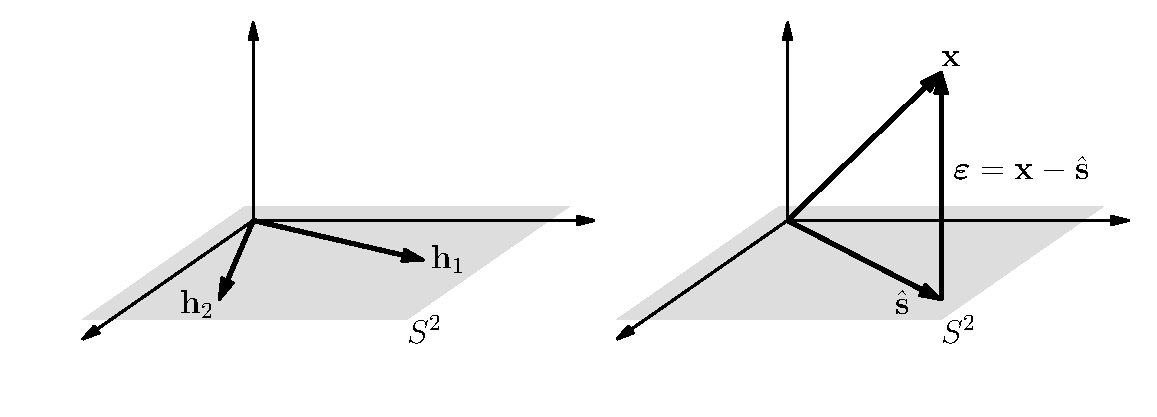
\includegraphics[width=0.8\textwidth]{figuras/ls_geometrical_interpretation.pdf}
\caption{\label{fig:ls_geometrical_interpretation} Interpretación geométrica del LSE. El vector de datos \(\x\) pertenece a \(R^3\) y el modelo de señal tiene una matriz \(\Hbf=[\h_1\,\h_2]\) con dos columnas de \(R^3\), las cuales generan el subespacio \(S^2\). El estimador \(\hat{\s}\) es el vector de \(S^2\) con distancia mínima al vector de datos \(\x\) y es la proyección ortogonal de \(\x\) en \(S^2\). Además, el error de estimación \(\bm{\epsilon}\) es el vector ortogonal a \(S^2\) y es la proyección de \(\x\) en el subespacio ortogonal a \(S^2\).}
\end{center}
\end{figure}
En la figura \ref{fig:ls_geometrical_interpretation} se muestra un ejemplo en donde el vector de datos \(\x\) tiene dimensión \(N=3\) y por lo tanto pertenece a \(R^3\) y el parámetro tiene dimensión \(p=2\) y de forma correspondiente, la matriz \(\Hbf\) tiene dos columnas \([\h_1\,\h_2]\) las cuales generan el subespacio \(S^2\).

La señal estimada, que es la proyección de \(\x\) en \(S^p\), esta dada por
\[
 \hat{\s}=\Hbf\hat{\thetabf}=\Hbf(\Hbf^T\Hbf)^{-1}\Hbf^T\x=\mathbf{P}\x,
\]
donde en la segunda identidad se empleó que el estimador está dado por la ecuación \ref{eq:ls_lls_estimator_vector}. La matriz \(\mathbf{P}=\Hbf(\Hbf^T\Hbf)^{-1}\Hbf^T\) tiene dimensiones \(N\times N\) y se llama \emph{matriz de proyección ortogonal} o simplemente \emph{matriz de proyección}. Tiene las siguientes características:
\begin{enumerate}
 \item Es simétrica: \(\mathbf{P}^T=\mathbf{P}\).
 \item Es idempotente: \(\mathbf{P}^2=\mathbf{P}\).
\end{enumerate}
La primer propiedad se muestra en el problema \ref{sec:problem_8_11}. El hecho de que debe ser idempotente se deduce de que \(\mathbf{P}\) aplicado a \(\mathbf{P}\x\) conduce al mismo vector, ya que \(\mathbf{P}\x\) ya pertenece a \(S^p\). Además, la matriz de proyección es singular, ya que es de dimensión \(N\times N\) y rango \(p\), como se muestra en el problema \ref{sec:problem_8_12}. Si esto no fuera cierto, \(\x\) podría obtenerse a partir de \(\hat{\s}\) mediante la inversión de \(\mathbf{P}\), lo cual es imposible debido a que infinitos \(\x\) tienen la misma proyección \(\hat{\s}\).

De la misma forma, el vector de error \(\bm{\epsilon}=\x-\hat{\s}=(\I-\mathbf{P})\x\) es la proyección de \(\x\) en el subespacio complemento o subespacio ortogonal al subespacio de la señal. Se puede verificar que \(\mathbf{P}^\perp=\I-\mathbf{P}\) también es una matriz de proyección. De la ecuación \ref{eq:ls_lls_min_error_vector} puede deducirse que el error mínimo es justamente
\[
  J_\textrm{mín}=\lVert\bm{\epsilon}\rVert^2.
\]
                                                                                                                                                                                                                                                                                                                                                                                                                                                                                                                                                                                                                                                                                                                                                                                                                                                                                                                                                                                                                                                                                                                                                                           
\section{Mínimos cuadrados de orden recursivo}

En muchos casos, el modelo de los datos es desconocido y debe asumirse. Por ejemplo, considérese un conjunto de datos \(x[n]\) que varía suavemente en \(n\), como se muestra en la figura \ref{fig:ls_example_8_6_data}.
\begin{figure}[!htb]
\begin{center}
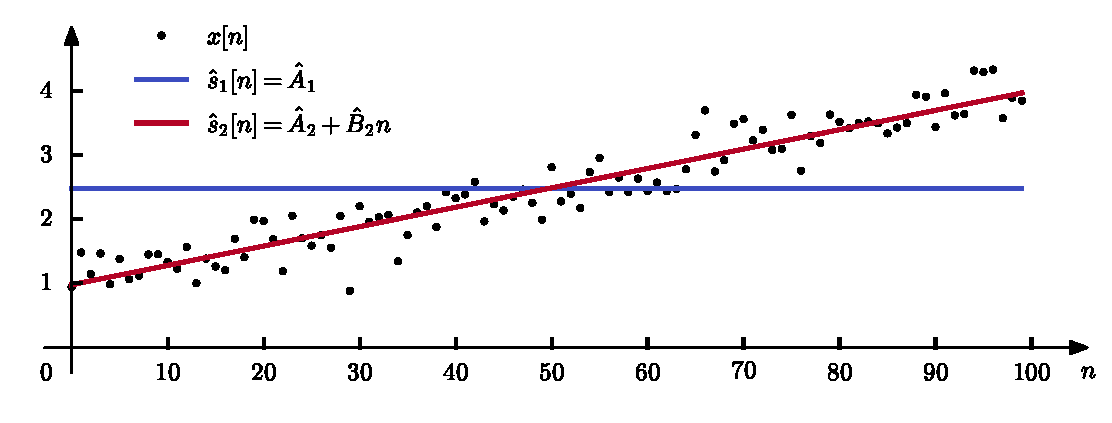
\includegraphics[width=0.98\textwidth]{figuras/example_8_6_data.pdf}
\caption{\label{fig:ls_example_8_6_data} Datos y LSE del modelo con un parámetro (constante) y dos parámetros (lineal). Los datos se generaron como \(s[n]=1+0.03n+w[n]\), donde \(w[n]\) es WGN con varianza \(\sigma^2=0.1\).}
\end{center}
\end{figure}                                                                                                                                                                                                                                                                                                                                                                                                                                                                                                                                                                                                                                                                                                                                                                                                                                                                                                                                                                                                                                                                                                                                                                           
Si el modelo de los datos es desconocido, se podría considerar un modelo constante, lineal, cuadrático o incluso de mayor orden en \(n\). Por ejemplo, los modelos constante y lineal son
\begin{align*}
 s_1[n]&=A\\
 s_2[n]&=A+Bn.
\end{align*}
Empleando el LSE con 
\[
 \Hbf_1=
 \begin{bmatrix}
  1\\
  1\\
  \vdots\\
  1
 \end{bmatrix}\qquad\qquad
 \Hbf_2=
 \begin{bmatrix}
  1 & 0\\
  1 & 1\\
  \vdots & \vdots\\
  1 & N-1
 \end{bmatrix}
\]
se obtienen los estimadores 
\[
 \hat{A}_1=\bar{x}
\]
para el modelo constante y
\begin{equation}\label{eq:ls_lls_line_fitting_estimator}
 \begin{aligned}
  \hat{A}_2&=\frac{2(2N-1)}{N(N+1)}\sum_{n=0}^{N-1}x[n]-\frac{6}{N(N+1)}\sum_{n=0}^{N-1}nx[n]\\
  \hat{B}_2&=-\frac{6}{N(N+1)}\sum_{n=0}^{N-1}x[n]+\frac{12}{N(N^2-1)}\sum_{n=0}^{N-1}nx[n],
 \end{aligned}
\end{equation}
para el modelo lineal, como se muestra en el problema de la sección \ref{sec:problem_8_13}.
La figura \ref{fig:ls_example_8_6_data} muestra que el modelo lineal con dos parámetros se ajusta mejor a los datos. Surge la duda de si debería agregarse un término cuadrático al modelo de los datos. Considerando que los datos están contaminados con ruido, puede ocurrir que al agregar mas parámetros el modelo se ajuste al ruido. Esta situación no es deseable, pero es inevitable si el modelo es desconocido. En la práctica, se elije el modelo mas simple que describa mejor a los datos. Considerando que el error LS mínimo se reduce al agregar mas parámetros, una estrategia podría ser incrementar la cantidad de parámetros hasta que el decrecimiento del error LS mínimo no sea significativo. 
\begin{figure}[!htb]
  \begin{minipage}[c]{0.5\textwidth}
    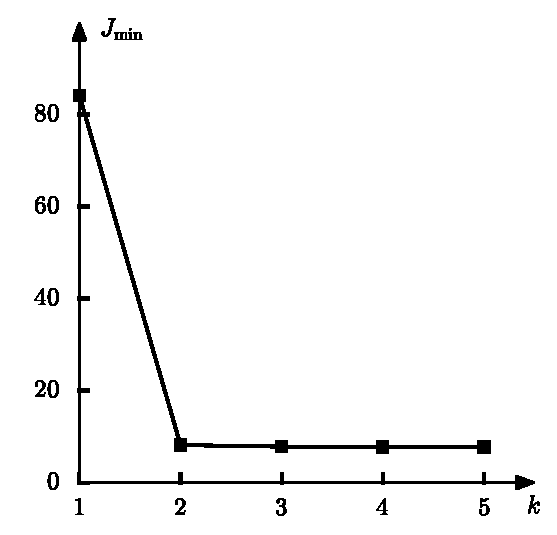
\includegraphics[width=\textwidth]{figuras/example_8_6_jmin.pdf}
  \end{minipage}\hfill
  \begin{minipage}[c]{0.4\textwidth}
    \caption{
      Efecto del número \(k\) de parámetros del modelo en el error LS mínimo \(J_\textrm{min}\). El error LS cae significativamente en \(k=2\). Al incrementar el número de parámetros mas allá de ese valor, la caída es pequeña, sugiriendo que el número de parámetros de la señal es efectivamente \(k=2\). 
    } \label{fig:ls_example_8_6_jmin}
  \end{minipage}
\end{figure}
En la figura \ref{fig:ls_example_8_6_jmin} se muestra el error LS mínimo \(J_\textrm{min}\) en función del número \(k\) de parámetros del modelo, que es un polinomio en \(n\) de grado \(k-1\). Los modelos \(s_1[n]\) y \(s_2[n]\) corresponden a \(k=1\) y \(k=2\). Se observa que un decrecimento grande de \(J_\textrm{min}\) ocurre con \(k=2\). Para ordenes mayores, la caída del error LS mínimo no es significativa, indicando que se está modelando además el ruido. En este ejemplo, los datos efectivamente son lineales en \(n\). En el caso en que \(A\) y \(B\) sean estimados de forma exacta, el error LS mínimo sería
\[
 J_\textrm{min}=J(A,\,B)=J(\hat{A},\,\hat{B})=\sum_{n=0}^{N-1}(x[n]-s[n])^2=\sum_{n=0}^{N-1}w^2[n]\approx N\sigma^2,
\]
y teniendo en cuenta que en este ejemplo \(N=100\) y \(\sigma^2=0.1\), resulta en \(J_\textrm{min}\approx10\). Esto se verifica en la figura \ref{fig:ls_example_8_6_jmin}, y se confirma que el modelo elegido es el apropiado.
                                                                                                                                                                                                                                                                                                                                                                                                                                                                                                                                                                                                                                                                                                                                                                                                                                                                                                                                                                                                                                                                                                                                                                                                                                                                                                                                                                                 
El ejemplo sugiere que es importante poder determinar el LSE para varios modelos de señal. La forma directa de hacerlo, es calcular el estimador para cada modelo empleando la ecuación \ref{eq:ls_lls_estimator_vector}. Sin embargo, la costo computacional puede reducirse empleando el enfoque LS de orden recursivo. Mediante este método, se actualiza el orden del modelo LSE en cada recursión. Específicamente, se calcula el LSE de un modelo con \(\Hbf\) de dimensiones \(N\times(k+1)\) a partir del LSE del modelo con \(\Hbf\) de dimensiones \(N\times k\). A continuación se resume la técnica y se incluye una deducción algebraica.

\subsection{Algoritmo LS de orden recursivo}

Sea la matriz de observación \(\Hbf_k\) de dimensiones \(N\times k\) y el LSE \(\thetabf_k\) correspondiente,
\begin{equation}\label{eq:ls_order_recursive_theta_k}
 \hat{\thetabf}_k=(\Hbf^T_k\Hbf_k)^{-1}\Hbf^T_k\x.
\end{equation}
El error LS mínimo del modelo basado en \(\Hbf_k\) es
\begin{equation}\label{eq:ls_order_recursive_jmin_k}
 J_{\min_k}=(\x-\Hbf_k\hat{\thetabf}_k)^T(\x-\Hbf_k\hat{\thetabf}_k).
\end{equation}
El orden del modelo se incrementa a \(k+1\) agregando una columna \(\h_{k+1}\) a la matriz de observación. Esto genera la nueva matriz de observación
\[
 \Hbf_{k+1}=
 \begin{bmatrix}
  \Hbf_k & \h_{k+1}
 \end{bmatrix}=
 \begin{bmatrix}
  N\times k & N\times 1
 \end{bmatrix}.
\]
La actualizaciones de \(\hat{\thetabf}_{k+1}\) es
\begin{equation}\label{eq:ls_order_recursive_theta_update}
\begingroup
\renewcommand*{\arraystretch}{2.6}
 \hat{\thetabf}_{k+1}=
 \begin{bmatrix}
  \hat{\thetabf}_k-\dfrac{(\Hbf^T_k\Hbf_k)^{-1}\Hbf^T_k\h_{k+1}\h_{k+1}^T\Pbf_k^\perp\x}{\h_{k+1}^T\Pbf_k^\perp\h_{k+1}}\\
  \dfrac{\h_{k+1}^T\Pbf_k^\perp\x}{\h_{k+1}^T\Pbf_k^\perp\h_{k+1}}
 \end{bmatrix}=
\endgroup
 \begin{bmatrix}
  k\times1\\
  1\times1
 \end{bmatrix}
\end{equation}
donde
\begin{equation}\label{eq:ls_order_recursive_p_k_definition}
 \Pbf_k^\perp=\I-\Hbf_k(\Hbf^T_k\Hbf_k)^{-1}\Hbf^T_k
\end{equation}
es la matriz de proyección sobre el subespacio ortogonal al generado por las columnas de \(\Hbf_k\). Para evitar invertir \(\Hbf^T_k\Hbf_k\) se define
\begin{equation}\label{eq:ls_order_recursive_D_k}
 \D_k=(\Hbf^T_k\Hbf_k)^{-1}
\end{equation}
y se emplea la fórmula recursiva
\begin{equation}\label{eq:ls_order_recursive_D_update}
\begingroup
\renewcommand*{\arraystretch}{2.6}
 \D_{k+1}=
 \begin{bmatrix}
  \D_k+\dfrac{\D_k\Hbf^T_k\h_{k+1}\h_{k+1}^T\Hbf_k\D_k}{\h_{k+1}^T\Pbf_k^\perp\h_{k+1}} & -\dfrac{\D_k\Hbf^T_k\h_{k+1}}{\h_{k+1}^T\Pbf_k^\perp\h_{k+1}}\\
  -\dfrac{\h_{k+1}^T\Hbf_k\D_k}{\h_{k+1}^T\Pbf_k^\perp\h_{k+1}}&\dfrac{1}{\h_{k+1}^T\Pbf_k^\perp\h_{k+1}}
 \end{bmatrix}=
\endgroup
 \begin{bmatrix}
  k\times k & k\times1\\
  1\times k & 1\times k
 \end{bmatrix}.
\end{equation}
El error LS mínimo se actualiza como
\begin{equation}\label{eq:ls_order_recursive_Jmin_update}
 J_{\min_{k+1}}=J_{\min_k}-\frac{(\h_{k+1}^T\Pbf_k^\perp\x)^2}{\h_{k+1}^T\Pbf_k^\perp\h_{k+1}}.
\end{equation}
El algoritmo no requiere la inversión de matrices. La recursión comienza calculando \(\hat{\thetabf}_1\), \(J_{\min_1}\) y \(\D_1\) empleando las ecuaciones \ref{eq:ls_order_recursive_theta_k}, \ref{eq:ls_order_recursive_jmin_k} y \ref{eq:ls_order_recursive_D_k} respectivamente. Las ecuaciones \ref{eq:ls_order_recursive_theta_update}, \ref{eq:ls_order_recursive_D_k} y \ref{eq:ls_order_recursive_Jmin_update} se denominan \emph{método de mínimos cuadrados de orden recursivo}. En la figura \ref{fig:ls_order_recursive_python} se muestra el código de una implementación del algoritmo. Ese código fue el empleado para obtener la gráfica de la figura \ref{fig:ls_example_8_6_jmin}. 
\begin{figure}[!htb]
\begin{center}
\lstinputlisting{figuras/ls_order_recursive.py}
\caption{\label{fig:ls_order_recursive_python} Implementación en el lenguaje Python del algoritmo LS de orden recursivo para el ejemplo del modelo de datos polinómico en \(n\). En la iteración \(k\)-ésima se calcula el estimador y el error LS mínimo en función de las estimaciones en el paso \(k-1\). Para que la implementación sea genérica, basta cambiar la especificación de la matriz \(\Hbf_1\) en el paso inicial y la columna \(\h_k\) a agregar a la matriz \(\Hbf_{k-1}\) en el paso \(k\)-ésimo.}
\end{center}
\end{figure}                                                                                                                                                                                                                                                                                                                                                                                                                                                                                                                                                                                                                                                                                                                                                                                                                                                                                                                                                                                                                                                                                                                                                                           

\paragraph{Deducción del algoritmo} Para deducir el algoritmo, se expresará el estimador, la matriz \(\D=(\Hbf^T\Hbf)^{-1}\) y el error LS mínimo en el paso \(k+1\) en función de sus valores en el paso \(k\). El estimador en el paso \(k+1\) es
\[
 \hat{\thetabf}_{k+1}=(\Hbf_{k+1}^T\Hbf_{k+1})^{-1}\Hbf_{k+1}^T\x.
\]
En el paso \(k+1\) se agrega la columna \(\h_{k+1}\) conocida a la matriz \(\Hbf_k\) del paso \(k\)-ésimo,
\[
 \Hbf_{k+1}=
 \begin{bmatrix}
  \Hbf_k & \h_{k+1}
 \end{bmatrix}.
\]
Por lo tanto,
\[
\begingroup
\renewcommand*{\arraystretch}{1.4}
 \Hbf_{k+1}^T\Hbf_{k+1}=
 \begin{bmatrix}
  \Hbf_k^T \\ \h_{k+1}^T
 \end{bmatrix}
 \begin{bmatrix}
  \Hbf_k & \h_{k+1}
 \end{bmatrix}=
 \begin{bmatrix}
  \Hbf_{k+1}^T\Hbf_{k+1} & \Hbf_{k+1}^T\h_{k+1}\\
  \h_{k+1}^T\Hbf_{k+1} & \h_{k+1}^T\h_{k+1}
 \end{bmatrix}=
 \begin{bmatrix}
  k\times k & k\times 1\\
  1\times k & 1\times 1
 \end{bmatrix}.
 \endgroup
\]
Cómo se explica en el apéndice \ref{ap:block_matrix_properties}, la matriz inversa de una matriz a bloques es
\[
 \begin{bmatrix}
  \A & \bbf\\
  \bbf^T & c
 \end{bmatrix}^{-1}=
 \begingroup
\renewcommand*{\arraystretch}{2.4}
 \begin{bmatrix}
  \left(\A-\dfrac{\bbf\bbf^T}{c}\right)^{-1} & -\dfrac{1}{c}\left(\A-\dfrac{\bbf\bbf^T}{c}\right)^{-1}\bbf\\
  -\dfrac{1}{c}\bbf^T\left(\A-\dfrac{\bbf\bbf^T}{c}\right)^{-1} & \dfrac{1}{c-\bbf^T\A^{-1}\bbf}
 \end{bmatrix},
 \endgroup
\]
donde se consideraron los elementos \((1,\,1)\), \((1,\,2)\) y \((2,\,1)\) de la matriz de la ecuación \ref{eq:block_matrix_inverse} y el elemento \((2,\,2)\) de la matriz de la ecuación \ref{eq:block_matrix_inverse_alt}, y por lo tanto,
\[
\begingroup
\renewcommand*{\arraystretch}{1.4}
 (\Hbf_{k+1}^T\Hbf_{k+1})^{-1}=
 \begin{bmatrix}
  \mathbf{E}_k & -\dfrac{\mathbf{E}_k\Hbf_{k+1}^T\h_{k+1}}{\h_{k+1}^T\h_{k+1}}\\
  -\dfrac{\h_{k+1}^T\Hbf_{k+1}\mathbf{E}_k}{\h_{k+1}^T\h_{k+1}} & \dfrac{1}{\h_{k+1}^T\h_{k+1}-\h_{k+1}^T\Hbf_k^T(\Hbf_k^T\Hbf_k)^{-1}\Hbf_k\h_{k+1}}
 \end{bmatrix},
 \endgroup
\]
donde se definió la matriz \(\mathbf{E}_k\) como la correspondiente al término \((\A-\bbf\bbf^T/c)^{-1}\), que es una matriz simétrica por ser \(\A\) simétrica. Empleando la identidad de Woodbury (ver la ecuación \ref{eq:woodbury_identity} del apéndice \ref{ap:woodbury_identity}), que indica que
\[
 \left(\A-\dfrac{\bbf\bbf^T}{c}\right)^{-1}=\A^{-1}+\dfrac{\A^{-1}\bbf\bbf^T\A^{-1}}{c-\bbf^T\A^{-1}\bbf},
\]
se tiene que
\begin{align*}
 \mathbf{E}_k&=(\Hbf_k^T\Hbf_k)^{-1}+\frac{(\Hbf_k^T\Hbf_k)^{-1}\Hbf_k^T\h_{k+1}\h_{k+1}^T\Hbf_k(\Hbf_k^T\Hbf_k)^{-1}}{\h_{k+1}^T\h_{k+1}-\h_{k+1}^T\Hbf_k(\Hbf_k^T\Hbf_k)^{-1}\Hbf_k^T\h_{k+1}}\\
  &=(\Hbf_k^T\Hbf_k)^{-1}+\frac{(\Hbf_k^T\Hbf_k)^{-1}\Hbf_k^T\h_{k+1}\h_{k+1}^T\Hbf_k(\Hbf_k^T\Hbf_k)^{-1}}{\h_{k+1}^T[\I-\Hbf_k(\Hbf_k^T\Hbf_k)^{-1}\Hbf_k^T]\h_{k+1}}\\
  &=(\Hbf_k^T\Hbf_k)^{-1}+\frac{(\Hbf_k^T\Hbf_k)^{-1}\Hbf_k^T\h_{k+1}\h_{k+1}^T\Hbf_k(\Hbf_k^T\Hbf_k)^{-1}}{\h_{k+1}^T\Pbf_k^\perp\h_{k+1}},
\end{align*}
en donde \(\Pbf_k^\perp=\I-\Pbf_k=\I-\Hbf_k(\Hbf_k^T\Hbf_k)^{-1}\Hbf_k^T\). Notar que el denominador de \(\mathbf{E}_k\) es el mismo que el elemento \((4,\,4)\) de \((\Hbf_{k+1}^T\Hbf_{k+1})^{-1}\). Definiendo \(\D_k=(\Hbf_k^T\Hbf_k)^{-1}\), se tiene que
\[
\begingroup
\renewcommand*{\arraystretch}{1.4}
 \D_{k+1}=(\Hbf_{k+1}^T\Hbf_{k+1})^{-1}=
 \begin{bmatrix}
  \mathbf{E}_k & -\dfrac{\mathbf{E}_k\Hbf_k^T\h_{k+1}}{\h_{k+1}^T\h_{k+1}}\\
  -\dfrac{\h_{k+1}^T\Hbf_k\mathbf{E}_k}{\h_{k+1}^T\h_{k+1}} & \dfrac{1}{\h_{k+1}^T\Pbf_k^\perp\h_{k+1}}
 \end{bmatrix}
 \endgroup
\]
con 
\[
 \mathbf{E}_k=\D_k+\frac{\D_k\Hbf_k^T\h_{k+1}\h_{k+1}^T\Hbf_k\D_k}{\h_{k+1}^T\Pbf_k^\perp\h_{k+1}}.
\]
Sustituyendo \(\mathbf{E}_k\) en los elementos de la anti-diagonal de \(\D_{k+1}\), que son transpuestos, se ve que
\begin{align*}
 \dfrac{\mathbf{E}_k\Hbf_k^T\h_{k+1}}{\h_{k+1}^T\h_{k+1}}&=\frac{\D_k\Hbf_k^T\h_{k+1}}{\h_{k+1}^T\h_{k+1}}+\frac{\D_k\Hbf_k^T\h_{k+1}\h_{k+1}^T\Hbf_k\D_k\Hbf_k^T\h_{k+1}}{(\h_{k+1}^T\h_{k+1})(\h_{k+1}^T\Pbf_k^\perp\h_{k+1})}\\
 &=\frac{\D_k\Hbf_k^T\h_{k+1}\h_{k+1}^T\Pbf_k^\perp\h_{k+1}+\D_k\Hbf_k^T\h_{k+1}\h_{k+1}^T\Hbf_k\D_k\Hbf_k^T\h_{k+1}}{(\h_{k+1}^T\h_{k+1})(\h_{k+1}^T\Pbf_k^\perp\h_{k+1})}\\
 &=\frac{\D_k\Hbf_k^T\h_{k+1}[\h_{k+1}^T\Pbf_k^\perp\h_{k+1}+\h_{k+1}^T\Hbf_k\D_k\Hbf_k^T\h_{k+1}]}{(\h_{k+1}^T\h_{k+1})(\h_{k+1}^T\Pbf_k^\perp\h_{k+1})}\\
 &\overset{(a)}{=}\frac{\D_k\Hbf_k^T\h_{k+1}[\h_{k+1}^T\Pbf_k^\perp\h_{k+1}+\h_{k+1}^T\Pbf_k\h_{k+1}]}{(\h_{k+1}^T\h_{k+1})(\h_{k+1}^T\Pbf_k^\perp\h_{k+1})}\\
 &=\frac{\D_k\Hbf_k^T\h_{k+1}[\h_{k+1}^T(\Pbf_k^\perp+\Pbf_k)\h_{k+1}]}{(\h_{k+1}^T\h_{k+1})(\h_{k+1}^T\Pbf_k^\perp\h_{k+1})}\\
 &\overset{(b)}{=}\frac{\D_k\Hbf_k^T\h_{k+1}}{\h_{k+1}^T\Pbf_k^\perp\h_{k+1}}\\
\end{align*}
donde en \((a)\) se consideró que \(\Pbf_k=\Hbf_k\D_k\Hbf_k^T\) y en \((b)\) que \(\Pbf_k^\perp+\Pbf_k=\I\). Finalmente se tiene que 
\begin{equation}\label{eq:ls_order_recursive_d_k_update}
\begingroup
\renewcommand*{\arraystretch}{2.4}
 \D_{k+1}=
 \begin{bmatrix}
  \D_k+\dfrac{\D_k\Hbf_k^T\h_{k+1}\h_{k+1}^T\Hbf_k\D_k}{\h_{k+1}^T\Pbf_k^\perp\h_{k+1}} & -\dfrac{\D_k\Hbf_k^T\h_{k+1}}{\h_{k+1}^T\Pbf_k^\perp\h_{k+1}}\\
  -\dfrac{\h_{k+1}^T\Hbf_k\D_k}{\h_{k+1}^T\Pbf_k^\perp\h_{k+1}} & \dfrac{1}{\h_{k+1}^T\Pbf_k^\perp\h_{k+1}}
 \end{bmatrix}
 \endgroup
 =\begin{bmatrix}
  k\times k & k\times 1\\
  1\times k & 1\times 1
 \end{bmatrix}. 
\end{equation}
El estimador es
\begin{align*}
 \hat{\thetabf}_{k+1}&=\D_{k+1}\Hbf_{k+1}^T\x\\
  &=\D_{k+1}
 \begingroup
 \renewcommand*{\arraystretch}{1.4}
  \begin{bmatrix}
  \Hbf_k^T\x \\ \h_{k+1}^T\x
  \end{bmatrix}
 \endgroup\\
 &=
 \begingroup
 \renewcommand*{\arraystretch}{2.4}
  \begin{bmatrix}
  \D_k\Hbf_k^T\x+\dfrac{\D_k\Hbf_k^T\h_{k+1}\h_{k+1}^T\Hbf_k\D_k\Hbf_k^T\x}{\h_{k+1}^T\Pbf_k^\perp\h_{k+1}}-\dfrac{\D_k\Hbf_k^T\h_{k+1}\h_{k+1}^T\x}{\h_{k+1}^T\Pbf_k^\perp\h_{k+1}}\\
  -\dfrac{\h_{k+1}^T\Hbf_k\D_k\Hbf_k^T\x}{\h_{k+1}^T\Pbf_k^\perp\h_{k+1}}+ \dfrac{\h_{k+1}^T\x}{\h_{k+1}^T\Pbf_k^\perp\h_{k+1}}
 \end{bmatrix}
 \endgroup\\
 &=
 \begingroup
 \renewcommand*{\arraystretch}{2.4}
  \begin{bmatrix}
  \hat{\thetabf}_k-\dfrac{\D_k\Hbf_k^T\h_{k+1}\h_{k+1}^T(\I-\Hbf_k\D_k\Hbf_k^T)\x}{\h_{k+1}^T\Pbf_k^\perp\h_{k+1}}\\
  \dfrac{\h_{k+1}^T(\I-\Hbf_k\D_k\Hbf_k^T)\x}{\h_{k+1}^T\Pbf_k^\perp\h_{k+1}}
 \end{bmatrix}
 \endgroup\\
 &=
 \begingroup
 \renewcommand*{\arraystretch}{2.4}
  \begin{bmatrix}
  \hat{\thetabf}_k-\dfrac{\D_k\Hbf_k^T\h_{k+1}\h_{k+1}^T\Pbf_k^\perp\x}{\h_{k+1}^T\Pbf_k^\perp\h_{k+1}}\\
  \dfrac{\h_{k+1}^T\Pbf_k^\perp\x}{\h_{k+1}^T\Pbf_k^\perp\h_{k+1}}
 \end{bmatrix}
 \endgroup\\
\end{align*}
Finalmente, la actualización del error LS mínimo es
\begin{align*}
 J_{\min_{k+1}}&=(\x-\Hbf_{k+1}\hat{\thetabf}_{k-1})^T(\x-\Hbf_{k+1}\hat{\thetabf}_{k-1})\\
   &=\x^T(\x-\Hbf_{k+1}\hat{\thetabf}_{k-1})-\hat{\thetabf}_{k-1}^T\Hbf_{k+1}^T(\x-\Hbf_{k+1}\hat{\thetabf}_{k-1})\\
   &\overset{(a)}{=}\x^T(\x-\Hbf_{k+1}\hat{\thetabf}_{k-1})-\hat{\thetabf}_{k-1}^T\Hbf_{k+1}^T\bm{\epsilon}_{k+1}\\
   &\overset{(b)}{=}\x^T\x-\x^T\Hbf_{k+1}\hat{\thetabf}_{k-1}\\
   &=\x^T\x-\x^T
 \begin{bmatrix}
  \Hbf_k & \h_{k+1}
 \end{bmatrix}
 \begingroup
 \renewcommand*{\arraystretch}{2.4}
  \begin{bmatrix}
  \hat{\thetabf}_k-\dfrac{\D_k\Hbf_k^T\h_{k+1}\h_{k+1}^T\Pbf_k^\perp\x}{\h_{k+1}^T\Pbf_k^\perp\h_{k+1}}\\
  \dfrac{\h_{k+1}^T\Pbf_k^\perp\x}{\h_{k+1}^T\Pbf_k^\perp\h_{k+1}}
 \end{bmatrix}
 \endgroup\\
 &=\x^T\x-\x^T\Hbf_k\hat{\thetabf}_k+\frac{\x^T\Hbf_k\D_k\Hbf_k^T\h_{k+1}\h_{k+1}^T\Pbf_k^\perp\x}{\h_{k+1}^T\Pbf_k^\perp\h_{k+1}}-\frac{\x^T\h_{k+1}\h_{k+1}^T\Pbf_k^\perp\x}{\h_{k+1}^T\Pbf_k^\perp\h_{k+1}}\\
 &\overset{(c)}{=}J_{\min_k}-\frac{\x^T(\I-\Hbf_k\D_k\Hbf_k^T)\h_{k+1}\h_{k+1}^T\Pbf_k^\perp\x}{\h_{k+1}^T\Pbf_k^\perp\h_{k+1}}\\
 &=J_{\min_k}-\frac{\x^T\Pbf_k^\perp\h_{k+1}\h_{k+1}^T\Pbf_k^\perp\x}{\h_{k+1}^T\Pbf_k^\perp\h_{k+1}}\\
 &=J_{\min_k}-\frac{(\h_{k+1}^T\Pbf_k^\perp\x)^2}{\h_{k+1}^T\Pbf_k^\perp\h_{k+1}},
\end{align*}
donde en \((a)\), \(\bm{\epsilon}_{k+1}=\x-\Hbf_{k+1}\hat{\thetabf}_{k-1}\) es el error de estimación en el paso \(k+1\), en \((b)\) se consideró el principio de ortogonalidad dado por la ecuación \ref{eq:ls_orthogonality_principle}, que indica que \(\Hbf_{k+1}^T\bm{\epsilon}_{k+1}=\textbf{0}\) y en \((c)\) que \(J_{\min_k}=\x^T\x-\x^T\Hbf_k\hat{\thetabf}_k\), como indica la identidad \((b)\) para el paso \(k+1\). En el problema \ref{sec:problem_8_14} se deriva el resultado empleando un enfoque geométrico.                                                                                                                                                                                                                                                                                                                                                                                                                                                                                                                                                                                                                                                                                                                                                                                                                                                                                                                                                                                                                                                                                                                                                                        
                                                                                                                                                                                                                                                                                                                                                                                                                                                                                                                                                                                                                                                                                                                                                                                                                                                                                                                                                                                                                                                                                                                                                                           
La matriz de proyección también puede ser actualizada de forma recursiva. Efectivamente, como
\[
 \Pbf_{k+1}=\Hbf_{k+1}(\Hbf_{k+1}^T\Hbf_{k+1})^{-1}\Hbf_{k+1}^T=\Hbf_{k+1}\D_{k+1}\Hbf_{k+1}^T,
\]
se puede emplear la ecuación de la actualización de \(\D_k\) dada por la ecuación \ref{eq:ls_order_recursive_d_k_update}. De esta forma,

\begin{align*}
 \Pbf_{k+1}&=
 \begin{bmatrix}
  \Hbf_k & \h_{k+1}
 \end{bmatrix}
 \renewcommand*{\arraystretch}{2.4}
 \begingroup
 \begin{bmatrix}
  \D_k+\dfrac{\D_k\Hbf_k^T\h_{k+1}\h_{k+1}^T\Hbf_k\D_k}{\h_{k+1}^T\Pbf_k^\perp\h_{k+1}} & -\dfrac{\D_k\Hbf_k^T\h_{k+1}}{\h_{k+1}^T\Pbf_k^\perp\h_{k+1}}\\
  -\dfrac{\h_{k+1}^T\Hbf_k\D_k}{\h_{k+1}^T\Pbf_k^\perp\h_{k+1}} & \dfrac{1}{\h_{k+1}^T\Pbf_k^\perp\h_{k+1}}
 \end{bmatrix}
 \endgroup
 \begin{bmatrix}
  \Hbf_k^T \\ \h_{k+1}^T
 \end{bmatrix}\\
 &=
 \begin{bmatrix}
  \Hbf_k & \h_{k+1}
 \end{bmatrix}
 \renewcommand*{\arraystretch}{2.4}
 \begingroup
 \begin{bmatrix}
  \D_k\Hbf_k^T+\dfrac{\D_k\Hbf_k^T\h_{k+1}\h_{k+1}^T\Hbf_k\D_k\Hbf_k^T}{\h_{k+1}^T\Pbf_k^\perp\h_{k+1}} -\dfrac{\D_k\Hbf_k^T\h_{k+1}\h_{k+1}^T}{\h_{k+1}^T\Pbf_k^\perp\h_{k+1}}\\
  -\dfrac{\h_{k+1}^T\Hbf_k\D_k\Hbf_k^T}{\h_{k+1}^T\Pbf_k^\perp\h_{k+1}} + \dfrac{\h_{k+1}^T}{\h_{k+1}^T\Pbf_k^\perp\h_{k+1}}
 \end{bmatrix}
 \endgroup\\
 &=\Hbf_k\D_k\Hbf_k^T+\dfrac{\Hbf_k\D_k\Hbf_k^T\h_{k+1}\h_{k+1}^T\Hbf_k\D_k\Hbf_k^T}{\h_{k+1}^T\Pbf_k^\perp\h_{k+1}}-\dfrac{\Hbf_k\D_k\Hbf_k^T\h_{k+1}\h_{k+1}^T}{\h_{k+1}^T\Pbf_k^\perp\h_{k+1}}\\
  &\qquad-\dfrac{\h_{k+1}\h_{k+1}^T\Hbf_k\D_k\Hbf_k^T}{\h_{k+1}^T\Pbf_k^\perp\h_{k+1}} + \dfrac{\h_{k+1}\h_{k+1}^T}{\h_{k+1}^T\Pbf_k^\perp\h_{k+1}}\\
 &=\Pbf_k+\dfrac{\Pbf_k\h_{k+1}\h_{k+1}^T\Pbf_k}{\h_{k+1}^T\Pbf_k^\perp\h_{k+1}}-\dfrac{\Pbf_k\h_{k+1}\h_{k+1}^T}{\h_{k+1}^T\Pbf_k^\perp\h_{k+1}}
  -\dfrac{\h_{k+1}\h_{k+1}^T\Pbf_k}{\h_{k+1}^T\Pbf_k^\perp\h_{k+1}} + \dfrac{\h_{k+1}\h_{k+1}^T}{\h_{k+1}^T\Pbf_k^\perp\h_{k+1}}
\end{align*}
resultando en 
\begin{equation}\label{eq:ls_order_recursive_P_update}
 \Pbf_{k+1}=\Pbf_k+\dfrac{(\I-\Pbf_k)\h_{k+1}\h_{k+1}^T(\I-\Pbf_k)}{\h_{k+1}^T(\I-\Pbf_k)\h_{k+1}}.
\end{equation}
Esta ecuación se llama \emph{matriz de proyección ortogonal recursiva}. En el problema de la sección \ref{sec:problem_8_18} se emplea para deducir la ecuación recursiva del error LS mínimo.

\section{Mínimos cuadrados secuencial}\label{sec:ls_sequential}

En las aplicaciones en donde hay que procesar muestras que se reciben una a una, es de interés poder actualizar el estimador cuando se observa una nueva muestra. Específicamente, supóngase que se determinó el LSE \(\hat{\thetabf}\) empleando las muestras \(\{x[0],\,x[1],\,\dots,\,x[N-1]\}\). Si se observa la muestra \(x[N]\), se desea actualizar \(\hat{\thetabf}\) en lugar de resolver la ecuación \ref{eq:ls_lls_estimator_vector} empleando todas las muestras. Este procedimiento se denomina \emph{mínimos cuadrados secuencial}.  

\subsection{Caso escalar}
                                                                                                                                                                                                                                                                                                                                                                                                                                                                                                                                                                                                                                                                                                                                                                                                                                                                                                                                                                                                                                                                                                                                                                           
\subsubsection{Ejemplo: nivel de DC en ruido no correlacionado}                                                                                                                                                                                                                                                                                                                                                                                                                                                                                                                                                                                                                                                                                                                                                                                                                                                                                                                                                                                                                                                                                                                                                                           
                                                                                                                                                                                                                                                                                                                                                                                                                                                                                                                                                                                                                                                                                                                                                                                                                                                                                                                                                                                                                                                                                                                                                                           
Se considera el problema de estimación del nivel de DC donde el ruido \(w[n]\) es no correlacionado de varianza \(\sigma_n^2\). Aplicando el enfoque de LS ponderado (ver el problema de la sección \ref{sec:problem_8_9}), si la matriz de ponderación \(\W\) es diagonal con \([\W]_{ii}=1/\sigma^2_i\), el LSE ponderado, como se calculó en el problema de la sección \ref{sec:problem_8_8} es  
\[
 \hat{A}[N-1]=\frac{\displaystyle\sum_{n=0}^{N-1}\frac{x[n]}{\sigma_n^2}}{\displaystyle\sum_{n=0}^{N-1}\frac{1}{\sigma_n^2}},
\]
donde el argumento de \(\hat{A}\) indica el índice de la última muestra observada en el calculo del estimador.
Sea \(\hat{A}[N]\) el estimador incluyendo una nueva muestra \(x[N]\). Para encontrar el LSE secuencial, se observa que 
\begin{align*}
 \hat{A}[N]&=\frac{\displaystyle\sum_{n=0}^{N}\frac{x[n]}{\sigma_n^2}}{\displaystyle\sum_{n=0}^{N}\frac{1}{\sigma_n^2}}\\
  &=\frac{\displaystyle\sum_{n=0}^{N-1}\frac{x[n]}{\sigma_n^2}+\frac{x[N]}{\sigma_N^2}}{\displaystyle\sum_{n=0}^{N-1}\frac{1}{\sigma_n^2}}\\
  &=\frac{\left(\displaystyle\sum_{n=0}^{N-1}\frac{1}{\sigma_n^2}\right)\hat{A}[N-1]}{\displaystyle\sum_{n=0}^{N}\frac{1}{\sigma_n^2}}+\frac{\displaystyle\frac{x[N]}{\sigma_N^2}}{\displaystyle\sum_{n=0}^{N}\frac{1}{\sigma_n^2}}\\
  &=\frac{\left(\displaystyle\sum_{n=0}^{N}\frac{1}{\sigma_n^2}-\frac{1}{\sigma_N^2}\right)\hat{A}[N-1]}{\displaystyle\sum_{n=0}^{N}\frac{1}{\sigma_n^2}}+\frac{\displaystyle\frac{x[N]}{\sigma_N^2}}{\displaystyle\sum_{n=0}^{N}\frac{1}{\sigma_n^2}}\\
  &=\hat{A}[N-1]-\frac{\dfrac{1}{\sigma_N^2}}{\displaystyle\sum_{n=0}^{N}\frac{1}{\sigma_n^2}}+\frac{\displaystyle\frac{x[N]}{\sigma_N^2}}{\displaystyle\sum_{n=0}^{N}\frac{1}{\sigma_n^2}}
\end{align*}
resultando en
\[
 \hat{A}[N]=\hat{A}[N-1]-\frac{\dfrac{1}{\sigma_N^2}}{\displaystyle\sum_{n=0}^{N}\frac{1}{\sigma_n^2}}(x[N]-\hat{A}[N-1])
\]
El nuevo estimador es igual al estimador previo mas un \emph{término de corrección}. El factor de ganancia que multiplica al término de corrección depende de la confianza en la nueva muestra. Si la nueva muestra es ruidosa o \(\sigma^2_N\to\infty\), el estimador previo no se corrige. En caso contrario, si la nueva muestra no tiene ruido o \(\sigma^2_N\to0\), \(\hat{A}[N]\to x[N]\), lo que significa que las muestras previas se descartan. Por lo tanto, el factor de ganancia representa la confianza en la nueva muestra relativa a la confianza de las muestras previas. 
Continuando con la interpretación del resultado, se sabe por el problema de la sección \ref{sec:problem_8_8} que                                                                                                                                                                                                                                                                                                                                                                                                                                                                                                                                                                                                                                                                                                                                                                                                                                                                                                                                                                                                                                                                                                                                                                           
\[
 \var(\hat{A}[N-1])=\frac{1}{\displaystyle\sum_{n=0}^{N-1}\frac{1}{\sigma_n^2}}.
\]                                                                                                                                                                                                                                                                y el factor de ganancia de la corrección \(N\)-ésima es
\begin{align*}
 K[N]&=\frac{\dfrac{1}{\sigma_N^2}}{\displaystyle\sum_{n=0}^{N}\frac{1}{\sigma_n^2}}\\
  &=\frac{\dfrac{1}{\sigma_N^2}}{\dfrac{1}{\sigma_N^2}+\displaystyle\sum_{n=0}^{N-1}\frac{1}{\sigma_n^2}}\\
  &=\frac{\dfrac{1}{\sigma_N^2}}{\dfrac{1}{\sigma_N^2}+\dfrac{1}{\var(\hat{A}[N-1])}}
\end{align*}
resultando en
\[
 K[N]=\frac{\var(\hat{A}[N-1])}{\var(\hat{A}[N-1])+\sigma_N^2}.
\]
Como \(0\leq K[N]\leq 1\), la corrección es grande si \(K[N]\) es grande, cosa que ocurre cuando \(\var(\hat{A}[N-1])\) es grande. Asimismo, si la varianza del estimador previo es pequeña, también lo es la corrección. El hecho de que la ganancia dependa de \(\var(\hat{A}[N-1])\) puede emplearse para encontrar una expresión recursiva, ya que 
\begin{align*}
 \var(\hat{A}[N])&=\frac{1}{\displaystyle\sum_{n=0}^{N}\frac{1}{\sigma_n^2}}\\
  &=\frac{1}{\dfrac{1}{\sigma_N^2}+\displaystyle\sum_{n=0}^{N-1}\frac{1}{\sigma_n^2}}\\
  &=\frac{1}{\dfrac{1}{\sigma_N^2}+\dfrac{1}{\var(\hat{A}[N-1])}}\\
  &=\frac{\var(\hat{A}[N-1])\sigma_N^2}{\var(\hat{A}[N-1])+\sigma_N^2}\\
  &=\frac{\var(\hat{A}[N-1])\left[\sigma_N^2+\var(\hat{A}[N-1])-\var(\hat{A}[N-1])\right]}{\var(\hat{A}[N-1])+\sigma_N^2}\\
  &=\left(1-\frac{\var(\hat{A}[N-1])}{\var(\hat{A}[N-1])+\sigma_N^2}\right)\var(\hat{A}[N-1])\\
  &=\left(1-K[N]\right)\var(\hat{A}[N-1]).
\end{align*}
Para calcular la ganancia de forma recursiva, se procede como sigue:
\paragraph{Actualización del estimador:}
\begin{equation}\label{eq:ls_sls_no_corraleted_noise_estimator}
 \hat{A}[N]=\hat{A}[N-1]+K[N](x[N]-\hat{A}[N-1])
\end{equation}
donde
\begin{equation}\label{eq:ls_sls_no_corraleted_noise_gain}
 K[N]=\frac{\var(\hat{A}[N-1])}{\var(\hat{A}[N-1])+\sigma_N^2}
\end{equation}
\paragraph{Actualización de la varianza:}
\begin{equation}\label{eq:ls_sls_no_corraleted_noise_variance}
 \var(\hat{A}[N])=\left(1-K[N]\right)\var(\hat{A}[N-1]).
\end{equation}                                                                                                                                                                                                                                                                                                                                                                                                                                                                                                                                                                                                                                                                                                                                                                                                                                                                                                                                                                                                                                                                                                                                                                           
Para comenzar la recursión, se parte de
\[
\begin{array}{rcl}
 \hat{A}[0] & = & x[0]\\
 \var(\hat{A}[0]) & = & \sigma_0^2.
\end{array}
\]
Luego se calcula \(K[1]\) con la ecuación \ref{eq:ls_sls_no_corraleted_noise_gain} y \(\hat{A}[1]\) con la ecuación \ref{eq:ls_sls_no_corraleted_noise_estimator}. Después se calcula \(\var(\hat{A}[1])\) con la ecuación \ref{eq:ls_sls_no_corraleted_noise_variance}. Continuando de esta forma, se calcula \(K[2]\), \(\hat{A}[2]\) y \(\var(\hat{A}[2])\) y así sucesivamente. Observar que en el proceso de calcular la ganancia de forma recursiva, también se obtiene una recursión para la varianza del LSE. Se puede mostrar que el error LS mínimo también puede calcularse recursivamente como
\begin{equation}\label{eq:ls_sls_no_corraleted_noise_jmin}
 J_{\min}[N]=J_{\min}[N-1]+\frac{\left(x[N]-\hat{A}[N-1]\right)^2}{\var(\hat{A}[N-1])+\sigma_N^2},
\end{equation}
como se hace en el problema de la sección \ref{sec:problem_8_19}.

\subsection{Caso vectorial}

A continuación se generaliza el cálculo del LSE secuencial para el caso en que el parámetro es vectorial. Considérese la minimización de la función \(J\) del error LS ponderado (ver el problema de la sección \ref{sec:problem_8_9}),
\begin{equation}\label{eq:ls_lls_criterion_weighted_vector}
 J=(\x-\Hbf\thetabf)^T\C^{-1}(\x-\Hbf\thetabf), 
\end{equation}
con \(\W=\C^{-1}\), donde \(\C\) es la matriz de covarianza del ruido de media nula. Las hipótesis del problema son las mismas que el BLUE (ver el problema de la sección \ref{sec:problem_6_13}). Como se encontró en el problema de la sección \ref{sec:problem_8_9} (ver también la ecuación \ref{eq:blue_estimator_vector}), el LSE ponderado es
\[
 \hat{\thetabf}=(\Hbf^T\C^{-1}\Hbf)^{-1}\Hbf^T\C^{-1}\x
\]
con matriz de covarianza
\[
 \C_{\hat{\thetabf}}=(\Hbf^T\C^{-1}\Hbf)^{-1}.
\]
dada por la ecuación \ref{eq:blue_estimator_covariance_vector}). Solo si \(\C\) es diagonal, es decir, el ruido es no correlacionado, \(\hat{\thetabf}\) puede ser calculado secuencialmente en el tiempo. Asumiendo que esto es así, sea
\begin{align*}
 \C[n] &= \operatorname{diag}(\sigma^2_0,\,\sigma^2_1,\,\dots,\,\sigma^2_n)\\
 \Hbf[n] &=
 \begin{bmatrix}
  \Hbf[n-1]\\
  \h^T[n]
 \end{bmatrix}=
 \begin{bmatrix}
  n\times p\\
  1\times p
 \end{bmatrix}\\
 \x[n] &= [\x[0]\;\x[1]\;\dots\;\x[n]] 
\end{align*}
y \(\hat{\thetabf}\) el LSE ponderado de \(\thetabf\) calculado a partir de \(\x[n]\) o \((n+1)\) muestras. El estimador del lote de datos (\emph{batch estimator}) es
\begin{equation}\label{eq:ls_sequential_estimator_batch}
 \hat{\thetabf}[n]=(\Hbf^T[n]\C^{-1}[n]\Hbf[n])^{-1}\Hbf^T[n]\C^{-1}[n]\x[n]
\end{equation}
con matriz de covarianza
\begin{equation}\label{eq:ls_sequential_covariance_batch}
 \C_{\hat{\thetabf}}=\bm{\Sigma}[n]=(\Hbf^T[n]\C^{-1}[n]\Hbf[n])^{-1}.
\end{equation}
Notar que \(\C[n]\) es la matriz de covarianza del ruido mientras que \(\bm{\Sigma}[n]\) es la matriz de covarianza del LSE. El estimador secuencial es
\paragraph{Actualización del estimador:}
\begin{equation}\label{eq:ls_sequential_estimator_update}
 \hat{\thetabf}[n]=\hat{\thetabf}[n-1]+\K[n]\left(x[n]-\h^T[n]\hat{\thetabf}[n-1]\right)
\end{equation}
donde
\begin{equation}\label{eq:ls_sequential_gain_update}
 \K[n]=\frac{\bm{\Sigma}[n-1]\h[n]}{\sigma_n^2+\h^T[n]\bm{\Sigma}[n-1]\h[n]}
\end{equation}
\paragraph{Actualización de la matriz de covarianza:}
\begin{equation}\label{eq:ls_sequential_covariance_update}
 \bm{\Sigma}[n]=(\I-\K[n]\h^T[n])\bm{\Sigma}[n-1]
\end{equation}
El factor de ganancia \(\K[n]\) es un vector \(p\times1\) y la matriz de covarianza \(\bm{\Sigma}[n]\) tiene dimensiones \(p\times p\). En la figura \ref{fig:sequential_lse} se resume el algoritmo. Para comenzar la recursión es necesario especificar valores iniciales de \(\hat{\thetabf}[n-1]\) y \(\bm{\Sigma}[n-1]\) de forma de calcular \(\K[n]\) con la ecuación \ref{eq:ls_sequential_gain_update} y luego \(\hat{\thetabf}[n]\) y \(\bm{\Sigma}[n]\) con las ecuaciones \ref{eq:ls_sequential_estimator_update} y \ref{eq:ls_sequential_covariance_update} respectivamente. Una forma de determinar los valores iniciales \(\hat{\thetabf}[n-1]\) y \(\bm{\Sigma}[n-1]\) es mediante las ecuaciones por lotes \ref{eq:ls_sequential_estimator_batch} y \ref{eq:ls_sequential_covariance_batch}, lo que requiere que \(\Hbf^T[n-1]\C^{-1}[n-1]\Hbf[n-1]\) sea invertible. Para que esto suceda, \(\Hbf[n-1]\) debe tener rango mayor o igual a \(p\). Como \(\Hbf[n-1]\) tiene dimensiones \(n\times p\), se debe cumplir que \(n\geq p\), asumiendo que las \(p\) columnas son linealmente independientes. Por lo tanto, el procedimiento para el cálculo de LS secuencial típicamente comienza determinando \(\hat{\thetabf}[p-1]\) y \(\bm{\Sigma}[p-1]\) empleando el estimador de lotes de las ecuaciones \ref{eq:ls_sequential_estimator_batch} y \ref{eq:ls_sequential_covariance_batch} (ya que \(\Hbf[p-1]\) tiene dimensiones \(p\times p\)) y luego se emplean las ecuaciones secuenciales \ref{eq:ls_sequential_estimator_update}, \ref{eq:ls_sequential_gain_update} y \ref{eq:ls_sequential_covariance_update} para \(n\geq p\). Un segundo método de inicializar la recursión es asignar valores a \(\hat{\thetabf}[-1]\) y \(\bm{\Sigma}[-1]\) y calcular el LS secuencial para \(n\geq0\). Esto tiene el efecto de sesgar el estimador hacia \(\hat{\thetabf}[-1]\). La forma usual de minimizar el efecto del sesgo es elegir \(\bm{\Sigma}[-1]\) grande o \(\bm{\Sigma}[-1]=\alpha\I\) con \(\alpha\) grande, los que implica dar poca confianza a \(\bm{\Sigma}[-1]\). El LSE para \(n\geq p\) resulta en el mismo estimador que al emplear el estimador por lotes si \(\alpha\to\infty\), como se muestra en el problema de la sección \ref{sec:problem_8_23}. Finalmente, el error LS mínimo también puede ser calculado secuencialmente como
\begin{equation}\label{eq:ls_sequential_jmin_update}
  J_{\min}[n]=J_{\min}[n-1]+\frac{(x[n]-\h^T[n]\hat{\thetabf}[n-1])^2}{\sigma_n^2+\h^T[n]\bm{\Sigma}[n-1]\h[n]}.
\end{equation}
El algoritmo de mínimos cuadrados secuencial es usualmente referido en la literatura como \emph{algoritmo de mínimos cuadrados recursivo} (\emph{recursive least squares}, RLS), como por ejemplo en el capítulo 10 de \cite{haykin2014adaptive}. 
A continuación se incluye la deducción de las ecuaciones \ref{eq:ls_sequential_estimator_update},  \ref{eq:ls_sequential_gain_update}, \ref{eq:ls_sequential_covariance_update} y \ref{eq:ls_sequential_jmin_update} del algoritmo LS secuencial.
\begin{figure}[!htb]
  \begin{minipage}[c]{0.53\textwidth}
    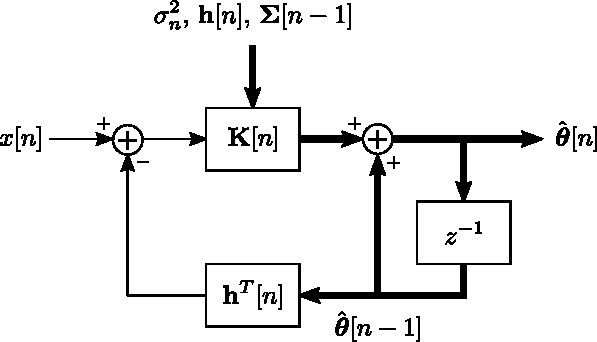
\includegraphics[width=\textwidth]{figuras/sequential_lse.pdf}
  \end{minipage}\hfill
  \begin{minipage}[c]{0.37\textwidth}
    \caption{
       Estimador por mínimos cuadrados secuencial. Las flechas gruesas indican procesamiento de vectores.
    }\label{fig:sequential_lse}
  \end{minipage}
\end{figure}
                                                                                                                                                                                                                                                                                                                                                                                                                                                                                                                                                                                                                                                                                                                                                                                                                                                                                                                                                                                                                                                                                                                                                                           
\paragraph{Deducción del algoritmo LS secuencial} El objetivo es expresar el estimador por lotes en el tiempo \(n\) en función del estimador en el tiempo \(n-1\). Para hacerlo, se parte de la matriz de covarianza del estimador \(\hat{\thetabf}[n]\), dada por la ecuación \ref{eq:ls_sequential_covariance_batch}, y se opera como sigue
\begin{align*}
 \bm{\Sigma}[n]&=\left(\Hbf^T[n]\C^{-1}[n]\Hbf[n]\right)^{-1}\\
  &=\left(
  \begin{bmatrix}
   \Hbf^T[n-1] & \h[n]
  \end{bmatrix}
  \begin{bmatrix}
   \C[n-1] & \mathbf{0}\\
   \mathbf{0}^T & \sigma_n^2
  \end{bmatrix}^{-1}
  \begin{bmatrix}
   \Hbf[n-1] \\ \h^T[n]
  \end{bmatrix}
  \right)^{-1}\\
 &\overset{(a)}{=}\left(
  \begin{bmatrix}
   \Hbf^T[n-1] & \h[n]
  \end{bmatrix}
  \begin{bmatrix}
   \C^{-1}[n-1] & \mathbf{0}\\
   \mathbf{0}^T & \dfrac{1}{\sigma_n^2}
  \end{bmatrix}
  \begin{bmatrix}
   \Hbf[n-1] \\ \h^T[n]
  \end{bmatrix}
  \right)^{-1}\\
  &\overset{(b)}{=}\left(\Hbf^T[n-1]\C^{-1}[n-1]\Hbf[n-1]+\frac{1}{\sigma_n^2}\h[n]\h^T[n]\right)^{-1}\\
  &=\left(\bm{\Sigma}^{-1}[n-1]+\frac{1}{\sigma_n^2}\h[n]\h^T[n]\right)^{-1}
\end{align*}
donde en \((a)\) se invirtió la matriz de covarianza del ruido teniendo en cuenta que es diagonal y en \((b)\) se realizaron las operaciones entre matrices. Empleando la identidad de Woodbury, dada por la ecuación \ref{eq:woodbury_identity} deducida en el apéndice \ref{ap:woodbury_identity}, se tiene que
\begin{align*}
 \bm{\Sigma}[n]&=\bm{\Sigma}[n-1]-\frac{\bm{\Sigma}[n-1]\h[n]\h^T[n]\bm{\Sigma}[n-1]}{\sigma_n^2+\h^T[n]\bm{\Sigma}[n-1]\h[n]}\\
  &=\left(\I-\frac{\bm{\Sigma}[n-1]\h[n]\h^T[n]}{\sigma_n^2+\h^T[n]\bm{\Sigma}[n-1]\h[n]}\right)\bm{\Sigma}[n-1].
\end{align*}
Definiendo 
\[
 \K[n]=\frac{\bm{\Sigma}[n-1]\h[n]}{\sigma_n^2+\h^T[n]\bm{\Sigma}[n-1]\h[n]}
\]
se obtiene que
\[
 \bm{\Sigma}[n]=\left(\I-\K[n]\h^T[n]\right)\bm{\Sigma}[n-1],
\]
que son respectivamente las ecuaciones \ref{eq:ls_sequential_gain_update} y \ref{eq:ls_sequential_covariance_batch} del algoritmo LS secuencial. Para encontrar la recursión del estimador, se parte del estimador por lotes, que está dado por la ecuación \ref{eq:ls_sequential_estimator_batch} y operando se ve que
\begin{align*}
 \hat{\thetabf}[n]&=(\Hbf^T[n]\C^{-1}[n]\Hbf[n])^{-1}\Hbf^T[n]\C^{-1}[n]\x[n]\\
  &=\bm{\Sigma}[n]
  \left(
  \begin{bmatrix}
   \Hbf^T[n-1] & \h[n]
  \end{bmatrix}
  \begin{bmatrix}
   \C[n-1] & \mathbf{0}\\
   \mathbf{0}^T & \sigma_n^2
  \end{bmatrix}^{-1}
  \begin{bmatrix}
   \x[n-1] \\ x[n]
  \end{bmatrix}
  \right)\\
 &\overset{(a)}{=}\left(\I-\K[n]\h^T[n]\right)\bm{\Sigma}[n-1]
  \left(
  \begin{bmatrix}
   \Hbf^T[n-1] & \h[n]
  \end{bmatrix}
  \begin{bmatrix}
   \C^{-1}[n-1] & \mathbf{0}\\
   \mathbf{0}^T & \dfrac{1}{\sigma_n^2}
  \end{bmatrix}
  \begin{bmatrix}
   \x[n-1] \\ x[n]
  \end{bmatrix}
  \right)\\
 &\overset{(b)}{=}\left(\I-\K[n]\h^T[n]\right)\bm{\Sigma}[n-1]\left(\Hbf^T[n-1]\C^{-1}[n-1]\x[n-1]+\frac{1}{\sigma_n^2}\h[n]x[n]\right),
\end{align*}
donde en \((a)\) se invirtió la matriz de covarianza del ruido y se sustituyó \(\bm{\Sigma}[n]\) por el resultado obtenido previamente y en \((b)\) se realizaron las operaciones entre matrices. Se encontrará una expresión para el término \(\Hbf^T[n-1]\C^{-1}[n-1]\x[n-1]\) considerando al estimador por lotes en el tiempo \(n-1\), que es
\begin{align*}
 \hat{\thetabf}[n-1]&=(\Hbf^T[n-1]\C^{-1}[n-1]\Hbf[n-1])^{-1}\Hbf^T[n-1]\C^{-1}[n-1]\x[n-1]\\
   &=\bm{\Sigma}[n-1]\Hbf^T[n-1]\C^{-1}[n-1]\x[n-1].
\end{align*} 
Por lo tanto,
\begin{equation}\label{eq:ls_sequential_deduction_tmp}
 \Hbf^T[n-1]\C^{-1}[n-1]\x[n-1]=\bm{\Sigma}^{-1}[n-1]\hat{\thetabf}[n-1],
\end{equation}
obteniendo que
\[
 \hat{\thetabf}[n]=\left(\I-\K[n]\h^T[n]\right)\bm{\Sigma}[n-1]\left(\bm{\Sigma}^{-1}[n-1]\hat{\thetabf}[n-1]+\frac{1}{\sigma_n^2}\h[n]x[n]\right),
\]
y desarrollando esta ecuación, se tiene que 
\[
 \hat{\thetabf}[n]=\hat{\thetabf}[n-1]+\frac{1}{\sigma_n^2}\bm{\Sigma}[n-1]\h[n]x[n]-\K[n]\h^T[n]\hat{\thetabf}[n-1]-\frac{1}{\sigma_n^2}\K[n]\h^T[n]\bm{\Sigma}[n-1]\h[n]x[n].
\]
De la definición de \(\K[n]\), se observa que el término \(\bm{\Sigma}[n-1]\h[n]\) en el segundo sumando puede expresarse como
\[
 \bm{\Sigma}[n-1]\h[n]=\K[n]\left(\sigma_n^2+\h^T[n]\bm{\Sigma}[n-1]\h[n]\right).
\]
Por lo tanto,
\begin{align*}
 \hat{\thetabf}[n]&=\hat{\thetabf}[n-1]+\frac{1}{\sigma_n^2}\K[n]\left(\sigma_n^2+\h^T[n]\bm{\Sigma}[n-1]\h[n]\right)x[n]-\K[n]\h^T[n]\hat{\thetabf}[n-1]\\
  &\qquad-\frac{1}{\sigma_n^2}\K[n]\h^T[n]\bm{\Sigma}[n-1]\h[n]x[n]\\
 &=\hat{\thetabf}[n-1]+\K[n]x[n]+\frac{1}{\sigma_n^2}\K[n]\h^T[n]\bm{\Sigma}[n-1]\h[n]x[n]-\K[n]\h^T[n]\hat{\thetabf}[n-1]\\
  &\qquad-\frac{1}{\sigma_n^2}\K[n]\h^T[n]\bm{\Sigma}[n-1]\h[n]x[n]\\
 &=\hat{\thetabf}[n-1]+\K[n]x[n]-\K[n]\h^T[n]\hat{\thetabf}[n-1], 
\end{align*}
resultando en
\[
 \hat{\thetabf}[n]=\hat{\thetabf}[n-1]+\K[n]\left(x[n]-\h^T[n]\hat{\thetabf}[n-1]\right),
\]
que es la ecuación \ref{eq:ls_sequential_estimator_update} del algoritmo LS secuencial.

También puede obtenerse una expresión recursiva para el error LS mínimo. El error mínimo por lotes es (ver ecuación \ref{eq:ls_lls_criterion_weighted_vector})                                                                                                                                                                                                                                                                                                                                                                                                                                                                                                                                                                                                                                                                                                                                                                                                                                                                                                                                                                                                                                                                                                                                                                                                                                                                                                                                                                                                                  \begin{align*}
 J_\textrm{min}[n]&=(\x[n]-\Hbf[n]\hat{\thetabf}[n])^T\C^{-1}[n](\x[n]-\Hbf[n]\hat{\thetabf}[n])\\
  &=\x^T[n]\C^{-1}[n](\x[n]-\Hbf[n]\hat{\thetabf}[n])-\hat{\thetabf}^T[n]\Hbf^T[n]\C^{-1}[n](\x[n]-\Hbf[n]\hat{\thetabf}[n])\\
  &\overset{(a)}{=}\x^T[n]\C^{-1}[n](\x[n]-\Hbf[n]\hat{\thetabf}[n]),
\end{align*}
donde en \((a)\) se tuvo en cuenta el principio de ortogonalidad, dado por la ecuación \ref{eq:ls_orthogonality_principle}, que indica que el error de estimación \(\bm{\epsilon}[n]=\x[n]-\Hbf[n]\hat{\thetabf}[n]\) es ortogonal al subespacio generado por las columnas de \(\Hbf[n]\) y por lo tanto \(\Hbf^T[n]\bm{\epsilon}[n]=\mathbf{0}\). Continuando,
\begin{align*}
 J_\textrm{min}[n]&=
  \begin{bmatrix}
   \x^T[n-1] & x[n]
  \end{bmatrix}
  \begin{bmatrix}
   \C^{-1}[n-1] & \mathbf{0}\\
   \mathbf{0}^T & \dfrac{1}{\sigma_n^2}
  \end{bmatrix}
  \begin{bmatrix}
   \x[n-1]-\Hbf[n-1]\hat{\thetabf}[n] \\ 
   x[n]-\h^T[n]\hat{\thetabf}[n]
  \end{bmatrix}\\
  &=\x^T[n-1]\C^{-1}[n-1]\left(\x[n-1]-\Hbf[n-1]\hat{\thetabf}[n] \right)+\frac{1}{\sigma_n^2}x[n]\left(x[n]-\h^T[n]\hat{\thetabf}[n]\right)\\
  &\overset{(a)}{=}\x^T[n-1]\C^{-1}[n-1]\left[\x[n-1]-\Hbf[n-1]\hat{\thetabf}[n-1]-\Hbf[n-1]\K[n]\left(x[n]-\h^T[n]\hat{\thetabf}[n-1]\right)\right]\\
   &\qquad+\frac{1}{\sigma_n^2}x[n]\left[x[n]-\h^T[n]\hat{\thetabf}[n-1]-\h^T[n]\K[n]\left(x[n]-\h^T[n]\hat{\thetabf}[n-1]\right)\right]\\
  &\overset{(b)}{=}\x^T[n-1]\C^{-1}[n-1]\left(\x[n-1]-\Hbf[n-1]\hat{\thetabf}[n-1]-\Hbf[n-1]\K[n]e[n]\right)\\
   &\qquad+\frac{1}{\sigma_n^2}x[n]\left(e[n]-\h^T[n]\K[n]e[n]\right)\\
  &=\x^T[n-1]\C^{-1}[n-1]\left(\x[n-1]-\Hbf[n-1]\hat{\thetabf}[n-1]\right)-\x^T[n-1]\C^{-1}[n-1]\Hbf[n-1]\K[n]e[n]\\
   &\qquad+\frac{1}{\sigma_n^2}x[n]\left(1-\h^T[n]\K[n]\right)e[n], 
\end{align*}
donde en \((a)\) usó la actualización de \(\hat{\thetabf}[n]\) dada por la ecuación \ref{eq:ls_sequential_estimator_update} obtenida previamente y en \((b)\) se definió \(e[n]=x[n]-\h^T[n]\hat{\thetabf}[n-1]\). Luego, observando que el primer sumando es \(J_\textrm{min}[n-1]\), se obtiene que
\begin{align*}
 J_\textrm{min}[n]&=J_\textrm{min}[n-1]-\x^T[n-1]\C^{-1}[n-1]\Hbf[n-1]\K[n]e[n]+\frac{1}{\sigma_n^2}x[n]\left(1-\h^T[n]\K[n]\right)e[n]\\
  &\overset{(a)}{=}J_\textrm{min}[n-1]-\hat{\thetabf}^T[n-1]\bm{\Sigma}^{-1}[n-1]\K[n]e[n]+\frac{1}{\sigma_n^2}x[n]\left(1-\h^T[n]\K[n]\right)e[n]\\
  &\overset{(b)}{=}J_\textrm{min}[n-1]-\frac{\hat{\thetabf}^T[n-1]\bm{\Sigma}^{-1}[n-1]\bm{\Sigma}[n-1]\h[n]e[n]}{\sigma_n^2+\h^T[n]\bm{\Sigma}[n-1]\h[n]}\\
   &\qquad+\frac{1}{\sigma_n^2}x[n]\left(1-\frac{\h^T[n]\bm{\Sigma}[n-1]\h[n]}{\sigma_n^2+\h^T[n]\bm{\Sigma}[n-1]\h[n]}\right)e[n]\\
  &\overset{(c)}{=}J_\textrm{min}[n-1]-\frac{\hat{\thetabf}^T[n-1]\h[n]e[n]}{\sigma_n^2+\h^T[n]\bm{\Sigma}[n-1]\h[n]}+\frac{x[n]e[n]}{\sigma_n^2+\h^T[n]\bm{\Sigma}[n-1]\h[n]}\\
  &=J_\textrm{min}[n-1]+\frac{\left(x[n]-\hat{\thetabf}^T[n-1]\h[n]\right)e[n]}{\sigma_n^2+\h^T[n]\bm{\Sigma}[n-1]\h[n]},
\end{align*}
donde en \((a)\) se sustituyó \(\x[n-1]^T\C^{-1}[n-1]\Hbf[n-1]\) empleando la ecuación \ref{eq:ls_sequential_deduction_tmp}, en \((b)\) se sustituyó \(\K[n]\) empleando la ecuación \ref{eq:ls_sequential_gain_update} deducida previamente y en \((c)\) se eliminaron las matrices inversas en el segundo sumando y se sacó denominador común en el término entre paréntesis del tercer sumando. Finalmente, notando que el término entre paréntesis es \(e[n]\), se concluye que
\[
 J_\textrm{min}[n]=J_\textrm{min}[n-1]+\frac{e^2[n]}{\sigma_n^2+\h^T[n]\bm{\Sigma}[n-1]\h[n]}.
\]

\section{Mínimos cuadrados restringidos}\label{sec:ls_constrained}
                                                                                                                                                                                                                                                                                                                                                                                                                                                                                                                                                                                                                                                                                                                                                                                                                                                                                                                                                                                                                                                                                                                                                                           
El problema de LS restringidos se aplica cuando hay que imponer restricciones a los parámetros a estimar. Un ejemplo típico es cuando se sabe a priori que algunos de ellos son iguales. Asúmase que el parámetro \(\thetabf\) esta sujeto a \(r<p\) restricciones lineaes. El conjunto de restricciones puede expresarse como
\begin{equation}\label{eq:ls_constrained_constrains}
 \A\thetabf=\bbf,
\end{equation}
donde \(\A\) es una matriz conocida de tamaño \(r\times p\) de rango completo \(r\) y \(\bbf\) es es un vector conocido \(r\times1\). Para encontrar el LSE sujeto a las restricciones lineales se emplea la técnica de los multiplicadores de Lagrange. El estimador \(\hat{\thetabf}_c\) restringido se obtiene minimizando el lagrangeano
\[
 J_c=(\x-\Hbf\thetabf)^T(\x-\Hbf\thetabf)+\bm{\lambda}^T(\A\thetabf-\bbf).
\]
Puede verificarse que al hacerlo, la solución es
\begin{equation}\label{eq:ls_constrained_estimator}
 \hat{\thetabf}_c=\hat{\thetabf}-(\Hbf^T\Hbf)^{-1}\A^T[\A(\Hbf^T\Hbf)^{-1}\A^T]^{-1}(\A\hat{\thetabf}-\bbf),
\end{equation}
donde \(\hat{\thetabf}=(\Hbf^T\Hbf)^{-1}\Hbf^T\x\) es el estimador sin restricciones.
                                                                                                                                                                                                                                                                                                                                                                                                                                                                                                                                                                                                                                                                                                                                                                                                                                                                                                                                                                                                                                                                                                                                                                           
\paragraph{Ejemplo: señal restringida} Supóngase que el modelo de la señal es
\[
 s[n]=\left\{ 
 \begin{array}{ll}
  \theta_1 & n=0\\
  \theta_2 & n=1\\
  0 & n=2\\
 \end{array}\right.
\]
y se observa \(\{x[0],\,x[1],\,x[2]\}\). En notación matricial el modelo se expresa como
\[
 \s=\Hbf\thetabf,\qquad\qquad\textrm{con}\qquad\qquad
 \Hbf=\begin{bmatrix}
  1 & 0\\ 0 & 1\\ 0 & 0
 \end{bmatrix}
 \qquad\textrm{y}\qquad
 \thetabf=
 \begin{bmatrix}
  \theta_1\\ \theta_2
 \end{bmatrix}.
\]
Observar que el vector señal
\[
 \s=
 \begin{bmatrix}
  \theta_1\\ \theta_2 \\ 0
 \end{bmatrix}.
\]
pertenece al plano mostrado en la figura \ref{fig:ls_constrained_signal}.
\begin{figure}[!htb]
\begin{center}
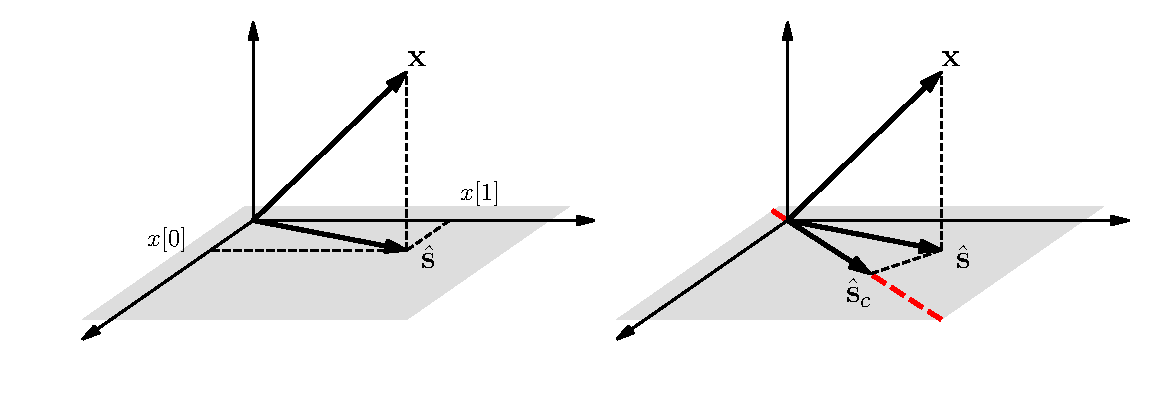
\includegraphics[width=0.8\textwidth]{figuras/ls_constrained_signal.pdf}
\caption{\label{fig:ls_constrained_signal} Mínimos cuadrados restringidos para el ejemplo de la señal restringida. En el caso sin restricciones (izquierda), la señal \(\hat{\s}\) estimada pertenece al subespacio generador por \(\Hbf\), que es el plano en gris. En el caso con restricciones (derecha) la señal \(\hat{\s}_c\) estimada pertenece al subespacio restringido, que está marcado en rojo, y es la proyección ortogonal de la señal estimada sin restricciones sobre éste.}
\end{center}
\end{figure}
Considerando que en este caso \(\Hbf^T\Hbf=\I\), el LSE sin restricciones es
\[
 \hat{\thetabf}=(\Hbf^T\Hbf)^{-1}\Hbf^T\x=
 \begin{bmatrix}
  x[0]\\ x[1]
 \end{bmatrix}
\]
y el estimador de la señal es
\[
 \hat{\s}=
 \begin{bmatrix}
  x[0]\\ x[1] \\ 0
 \end{bmatrix}.
\]
Asúmase ahora que se sabe a priori que \(\thetabf_1=\thetabf_2\). En términos de la ecuación \ref{eq:ls_constrained_constrains} de la restricciones, esta restricción se escribe como
\[
 \begin{bmatrix}
  1 & -1
 \end{bmatrix}
 \thetabf=0,
 \qquad\qquad\Rightarrow\qquad\qquad
 \A=
 \begin{bmatrix}
  1 & -1
 \end{bmatrix}
 \qquad\textrm{y}\qquad
 \bbf=0.
\]
De la ecuación \ref{eq:ls_constrained_estimator} se deduce que estimador con restricciones es
\begin{align*}
 \hat{\thetabf}_c&=\hat{\thetabf}-(\Hbf^T\Hbf)^{-1}\A^T[\A(\Hbf^T\Hbf)^{-1}\A^T]^{-1}(\A\hat{\thetabf}-\bbf)\\
   &\overset{(a)}{=}\hat{\thetabf}-\A^T(\A\A^T)^{-1}\A\hat{\thetabf}\\
   &=[\I-\A^T(\A\A^T)^{-1}\A]\hat{\thetabf}\\
   &=\left(
   \begin{bmatrix}
    1 & 0\\ 0 & 1
   \end{bmatrix}-
   \frac{1}{2}
   \begin{bmatrix}
    1 & -1\\ -1 & 1
   \end{bmatrix}
   \right)
   \begin{bmatrix}
    x[0] \\ x[1]
   \end{bmatrix}\\
   &=
   \begingroup
   \renewcommand*{\arraystretch}{2}
   \begin{bmatrix}
    \dfrac{1}{2} & \dfrac{1}{2}\\ \dfrac{1}{2} & \dfrac{1}{2}
   \end{bmatrix}
   \endgroup
   \begin{bmatrix}
    x[0] \\ x[1]
   \end{bmatrix},
\end{align*}
donde en \((a)\) se tuvo en cuenta que \(\Hbf^T\Hbf=\I\) y \(\bbf=0\). Esto resulta en 
\[
 \renewcommand*{\arraystretch}{2}
 \hat{\thetabf}_c=
 \begin{bmatrix}
  \dfrac{1}{2}(x[0] + x[1])\\
  \dfrac{1}{2}(x[0] + x[1])
 \end{bmatrix}
\]
y la señal estimada restringida es
\[
 \renewcommand*{\arraystretch}{2}
 \hat{\s}_c=\Hbf\hat{\thetabf}_c=
 \begin{bmatrix}
  \dfrac{1}{2}(x[0] + x[1])\\
  \dfrac{1}{2}(x[0] + x[1])\\
  0
 \end{bmatrix}
\]
como se muestra en la figura \ref{fig:ls_constrained_signal}. En este problema, se podría haber incluido la restricción en el modelo de la señal como
\[
 s[n]=\left\{ 
 \begin{array}{ll}
  \theta & n=0\\
  \theta & n=1\\
  0 & n=2\\
 \end{array}\right.
\]
que en forma matricial es
\[
 \s=
 \begin{bmatrix}
  1\\ 1\\ 0
 \end{bmatrix}
 \thetabf
\]
y \(\s\) debe pertenecer al subespacio restringido generado por el vector \([1\,1\,0]^T\) indicado en la figura \ref{fig:ls_constrained_signal}. La señal estimada restringida \(\hat{\s}_c\) puede obtenerse como la proyección de la señal estimada sin restricciones sobre el subespacio restringido. Ver el problema de la sección \ref{sec:problem_8_24}.

\section{Mínimos cuadrados no lineales}\label{sec:least_squares_nonlineal}  

Mediante el procedimiento de mínimos cuadrados, el parámetro \(\thetabf\) del modelo se determina minimizando el error LS
\[
 J=(\x-\s(\thetabf))^T(\x-\s(\thetabf)),
\]
donde \(\s(\thetabf)\) es el modelo de señal de los datos \(\x\), cuya dependencia del parámetro \(\thetabf\) se muestra explícitamente. Notar que si \(\x-\s(\thetabf)\sim\mathcal{N}(\mathbf{0},\,\sigma^2\I)\), el LSE es también el MLE, ya que el error \(J\) es el exponente de la función de verosimilitud (ver el capítulo \ref{ch:mle}). En el problema LS lineal, la señal se expresa como \(\s(\thetabf)=\Hbf\thetabf\). En el caso general, \(\s(\thetabf)\) es una función no lineal de dimensión \(N\) y no puede expresarse de esa forma. En esta situación, la minimización de \(J\) es mucho mas difícil o incluso, imposible. En la práctica, el cálculo del LSE no lineal se basa en enfoques iterativos y sufre las mismas limitaciones de la determinación del MLE mediante métodos numéricos. El método mas eficaz de búsqueda en una grilla solo es viable si la dimensión \(p\) de \(\thetabf\) es pequeña.                                                                                                                                                                                                                                                                                                                                                                                                                                                                                                                                                                                                                                                                                                                                                                                                                                                                                                                                                                                                                                                                                                                                                                               
                                                                                                                                                                                                                                                                                                                                                                                                                                                                                                                                                                                                                                                                                                                                                                                                                                                                                                                                                                                                                                                                                                                                                                           
Hay algunos métodos para reducir la complejidad del problema LS no lineal que pueden emplearse en algunos pocos casos específicos. Uno es la \emph{transformación de los parámetros}, que consiste en buscar una transformación uno a uno de \(\thetabf\) que produzca un modelo lineal de señal en un nuevo espacio. Específicamente, se busca un función \(\g\) de dimensión \(p\) de forma que el parámetro transformado \(\alphabf=\g(\thetabf)\) produzca un modelo lineal de señal, es decir,
\[
 \s(\thetabf(\alphabf))=\s(\g^{-1}(\alphabf))=\Hbf\alphabf.
\]
De esta forma, el LSE lineal de \(\alphabf\) se obtiene mediante la ecuación \ref{eq:ls_lls_estimator_vector}
y luego, el LSE no lineal de \(\thetabf\) se obtiene como \(\hat{\thetabf}=\g^{-1}(\hat{\alphabf})\). Este método se basa en la propiedad de que la minimización puede realizarse en cualquier espacio transformado obtenido mediante una transformación uno a uno y luego aplicar la transformación inversa para volver al espacio original, como se muestra en el problema de la sección \ref{sec:problem_8_26}. Otro método para reducir la complejidad es el de la \emph{separación de parámetros}. En este caso, se aprovecha el hecho de que si bien el modelo es no lineal, podría ser lineal en alguno de los parámetros. En el problema de la sección \ref{sec:problem_8_1} se explica la técnica. Una situación en donde esto ocurre es en el ejemplo de la sección \ref{sec:mle_sinusoidal_parameters} y también en el problema de la sección \ref{sec:problem_8_28}.

A continuación se desarrolla el enfoque para resolver el problema LS no lineal general empleando el método numérico de Newthon-Raphson. El error LS a minimizar es
\[
 J=(\x-\s(\thetabf))^T(\x-\s(\thetabf))=\sum_{n=0}^{N-1}(x[n]-s[n])^2.
\]
Las condiciones necesarias pueden obtenerse diferenciando \(J\), y son 
\[
 \frac{\partial J}{\partial\theta_j}=-2\sum_{i=0}^{N-1}(x[i]-s[i])\frac{\partial s[i]}{\partial\theta_j}=0,
 \qquad\qquad j=1,\,\dots,\,p.
\]
Si se define la matriz jacobiana \(N\times p\) como
\[
 \left[\frac{\partial \s(\thetabf)}{\partial\thetabf}\right]_{ij}=\frac{\partial s[i]}{\partial\theta_j}
 \qquad\qquad
 \begin{array}{lcl}
  i&=&0,\,\dots,\,N-1\\
  j&=&1,\,\dots,\,p
 \end{array}
\]
las condiciones necesarias quedan
\begin{equation}\label{eq:ls_nlls_deduction_tmp}
 \sum_{i=0}^{N-1}(x[i]-s[i])\left[\frac{\partial \s(\thetabf)}{\partial\thetabf}\right]_{ij}=0,
 \qquad\qquad j=1,\,\dots,\,p,
\end{equation}
que en forma matricial puede escribirse como
\[
 {\frac{\partial \s(\thetabf)}{\partial\thetabf}}^T(\x-\s(\thetabf))=\mathbf{0},
\]
y consiste en un sistema de \(p\) ecuaciones no lineales.
Observar que en el caso en que el modelo de la señal es lineal con el parámetro, \(\s(\thetabf)=\Hbf\thetabf\), de forma que 
\[
 s[i]=[\Hbf\thetabf]_i=\sum_{j=1}^p h_{ij}\theta_j\qquad\qquad\Rightarrow\qquad\qquad
 \frac{\partial s[i]}{\partial\theta_j}=h_{ij},
\]
resultando en que \(\partial\s(\thetabf)/\partial\thetabf=\Hbf\), las condiciones necesarias quedan
\[
 \Hbf^T(\x-\Hbf\hat{\thetabf})=\mathbf{0}\qquad\Rightarrow\qquad
 \Hbf^T\Hbf\hat{\thetabf}=\Hbf^T\x\qquad\Rightarrow\qquad
 \hat{\thetabf}=(\Hbf^T\Hbf)^{-1}\Hbf^T\x,
\]
que es el LSE usual lineal. El sistema no lineal de ecuaciones puede resolverse mediante el método iterativo de Newton-Raphson (ver la sección 7.7 de \cite{kay93fundamentals}). La función a resolver es
\begin{equation}\label{eq:ls_nlls_deduction_g}
 \g(\thetabf)={\frac{\partial \s(\thetabf)}{\partial\thetabf}}^T(\x-\s(\thetabf)),
\end{equation}
por lo que la iteración de Newton-Raphson es
\begin{equation}\label{eq:ls_nlls_deduction_iteration_tmp}
 \thetabf_{k+1}=\thetabf_{k}-\left(\frac{\partial\g(\thetabf)}{\partial\thetabf}\right)^{-1}\g(\thetabf)\bigg|_{\thetabf=\thetabf_k}. 
\end{equation}
Para encontrar la matriz jacobiana de \(\g\), que es en realidad la matriz hessiana escalada de \(J\), se tiene en cuenta que el elemento \(i\)-esimo de \(\g\) es (ver la ecuación \ref{eq:ls_nlls_deduction_tmp})
\[
 [\g(\thetabf)]_i=\sum_{n=0}^{N-1}(x[n]-s[n])\frac{\partial s[n]}{\partial\theta_i},
 \qquad\qquad i=1,\,\dots,\,p,
\]
y por lo tanto
\begin{align*}
 \frac{\partial[\g(\thetabf)]_i}{\partial\theta_j}&=\frac{\partial}{\partial\theta_j}\left[\sum_{n=0}^{N-1}(x[n]-s[n])\frac{\partial s[n]}{\partial\theta_i}\right]\\
  &=\sum_{n=0}^{N-1}\left[(x[n]-s[n])\frac{\partial^2 s[n]}{\partial\theta_i\partial\theta_j}-\frac{\partial s[n]}{\partial\theta_i}\frac{\partial s[n]}{\partial\theta_j}\right].
\end{align*}
Para expresar esto de forma mas sucinta, sea
\begin{equation}\label{eq:ls_nlls_deduction_H}
 [\Hbf(\thetabf)]_{ij}=\left[\frac{\partial \s(\thetabf)}{\partial\thetabf}\right]_{ij}=\frac{\partial s[i]}{\partial\theta_j}
 \qquad\qquad
 \begin{array}{lcl}
  i&=&0,\,\dots,\,N-1\\
  j&=&1,\,\dots,\,p
 \end{array}, 
\end{equation}
y
\begin{equation}\label{eq:ls_nlls_deduction_G}
 [\G_n(\thetabf)]_{ij}=\frac{\partial^2s[n]}{\partial\theta_i\partial\theta_j}
 \qquad\qquad
 \begin{array}{lcl}
  i&=&0,\,\dots,\,p\\
  j&=&1,\,\dots,\,p
 \end{array}. 
\end{equation}
De esta forma
\begin{align*}
 \frac{\partial[\g(\thetabf)]_i}{\partial\theta_j}&=\sum_{n=0}^{N-1}\left[(x[n]-s[n])[\G_n(\thetabf)]_{ij}-[\Hbf(\thetabf)]_{ni}[\Hbf(\thetabf)]_{nj}\right]\\
  &=\sum_{n=0}^{N-1}[\G_n(\thetabf)]_{ij}(x[n]-s[n])-\sum_{n=0}^{N-1}[\Hbf^T(\thetabf)]_{in}[\Hbf(\thetabf)]_{nj}\\
  &=\sum_{n=0}^{N-1}[\G_n(\thetabf)]_{ij}(x[n]-s[n])-[\Hbf^T(\thetabf)\Hbf(\thetabf)]_{ij},
\end{align*}
resultando en que
\begin{equation}\label{eq:ls_nlls_deduction_g_jacobian}
  \frac{\partial\g(\thetabf)}{\partial\thetabf}=\sum_{n=0}^{N-1}\G_n(\thetabf)(x[n]-s[n])-\Hbf^T(\thetabf)\Hbf(\thetabf)
\end{equation}
Finalmente, sustituyendo las ecuaciones \ref{eq:ls_nlls_deduction_g} y \ref{eq:ls_nlls_deduction_g_jacobian} en la ecuación \ref{eq:ls_nlls_deduction_iteration_tmp} se obtiene que la iteración de Newton-Raphson para encontrar el estimador LS no lineal es
\begin{equation}\label{eq:ls_nlls_estimator_nr}
 \thetabf_{k+1}=\thetabf_{k}+\left(\Hbf^T(\thetabf_k)\Hbf(\thetabf_k)-\sum_{n=0}^{N-1}\G_n(\thetabf_k)(x[n]-s[n])\right)^{-1}\Hbf^T(\thetabf_k)(\x-\s(\thetabf_k)), 
\end{equation}
donde \(\Hbf(\thetabf)\) está dada por la ecuación \ref{eq:ls_nlls_deduction_H} y \(\G_n(\thetabf)\) por la ecuación \ref{eq:ls_nlls_deduction_G}, que son las derivadas parciales primera y segunda de la señal respecto a los parámetros. Es interesante notar que en caso de un modelo lineal, \(\s(\thetabf)=\Hbf\thetabf\), se cumple que \(\Hbf(\thetabf)=\Hbf\) y \(\G_n(\thetabf)=\mathbf{0}\), y por lo tanto
\begin{align*}
 \thetabf_{k+1}&=\thetabf_{k}+(\Hbf^T\Hbf)^{-1}\Hbf^T(\x-\Hbf\thetabf_k)\\
  &=(\Hbf^T\Hbf)^{-1}\Hbf^T\x.
\end{align*}
Esto indica que la convergencia se alcanza en un solo paso, y se debe a que la naturaleza cuadrática del error \(J\) resulta en una función \(\g(\thetabf)\) lineal. Es esperable que para modelos de señal aproximadamente lineales, la convergencia sea rápida.

\section{Ejemplos de procesamiento de señales}

Se incluyen a continuación algunos ejemplos en procesamiento de señales donde se emplea el LSE. En estas aplicaciones, el estimador MVU no puede obtenerse. Adicionalmente, la caracterización estadística del ruido puede no conocerse, e incluso si es conocida, el estimador MLE es generalmente muy complicado de calcular.

\subsection{Ejemplo: diseño de filtros digitales}\label{sec:ls_example_digital_filter_design}

Un problema común en procesamiento de señales es el diseño de un filtro digital cuya respuesta en frecuencia cumpla ciertas especificaciones. Alternativamente, se puede intentar hacer coincidir la respuesta al impulso con la respuesta al impulso deseada, y es el enfoque examinado en el presente ejemplo. Un filtro de respuesta al impulso infinita (\emph{infinite impulse response}, IIR) tiene función de transferencia
\begin{align*}
 \mathcal{H}(z)&=\frac{\mathcal{B}(z)}{\mathcal{A}(z)}\\
   &=\frac{b[0]+b[1]z^{-1}+\dots+b[q]z^{-q}}{1+a[1]z^{-1}+\dots+a[p]z^{-p}}.
\end{align*}
Si la respuesta en frecuencia deseada es \(H_d(f)=\mathcal{H}_d(e^{j2\pi f})\), su transformada de Fourier es la respuesta al impulso deseada,
\[
 h_d[n]=\mathcal{F}^{-1}\{H_d(f)\}.
\]
La respuesta al impulso de filtro es una ecuación en diferencias recursiva que se obtiene aplicando la transformada \(z\) inversa a \(\mathcal{H}(z)\). Para hacerlo, se multiplica por el denominador a ambos lados de la igualdad de la función de transferencia,
\[
 \mathcal{H}(z)+a[1]\mathcal{H}(z)z^{-1}+\dots+a[p]\mathcal{H}(z)z^{-p}=b[0]+b[1]z^{-1}+\dots+b[q]z^{-q}
\]
y al aplicar la transformada \(z\) inversa, se obtiene que 
\[
 h[n]+a[1]h[n-1]+\dots+a[p]h[n-p]=b[0]\delta[n]+b[1]\delta[n-1]+\dots+b[q]\delta[n-q],
\]
donde se tuvo en cuenta que
\[
 \delta[n-n_0]\overset{\mathcal{Z}}{\longleftrightarrow}z^{-n_0}
 \qquad\qquad\textrm{y}\qquad\qquad
 \delta[n-n_0]*h[n]=h[n-n_0]\overset{\mathcal{Z}}{\longleftrightarrow}z^{-n_0}\mathcal{H}(z).
\]
Despejando \(h[n]\), la expresión recursiva de la respuesta al impuso queda
\[
 h[n]=\left\{
 \begin{array}{ll}
  \displaystyle-\sum_{k=1}^{p}a[k]h[n-k]+\sum_{k=0}^qb[k]\delta[n-k] & n\geq0\\
  0 & n<0.
 \end{array}\right. 
\]
La solución directa mediante LS sería elegir los coeficientes \(\{a[k],\,b[k]\}\) de forma de minimizar
\[
 J=\sum_{n=0}^{N-1}(h_d[n]-h[n])^2,
\]
donde \(N\) es un entro suficientemente grande de forma que \(h[n]\) ya se haya extinguido y sea esencialmente nula. Notar que \(h_d[n]\) son los datos y \(h[n]\) es el modelo de la señal. El ruido en los datos se atribuye a error de modelado, por lo que su caracterización estadística es desconocida. Desafortunadamente, este enfoque produce un problema LS no lineal (ver el problema de la sección \ref{sec:problem_8_28}). Como ejemplo, si
\[
 \mathcal{H}(z)=\frac{b[0]}{1+a[1]z^{-1}},
\]
se tiene que
\[
 h[n]=\left\{
 \begin{array}{ll}
  b[0](-a[1])^n & n\geq0\\
  0 & n<0.
 \end{array}\right. 
\]
y
\[
 J=\sum_{n=0}^{N-1}(h_d[n]-b[0](-a[1])^n)^2,
\]
que es fuertemente no lineal en \(a[1]\). De hecho, es la presencia del denominador \(\mathcal{A}(z)\) que produce que el error LS no sea cuadrático. Para evitar este problema, se puede filtrar \(h_d[n]\) y \(h[n]\) con \(\mathcal{A}(z)\) de forma de cancelar el denominador de \(\mathcal{H}(z)\), como se muestra en la figura \ref{fig:example_8_11_esquema}.
\begin{figure}[!htb]
  \begin{minipage}[c]{0.7\textwidth}
    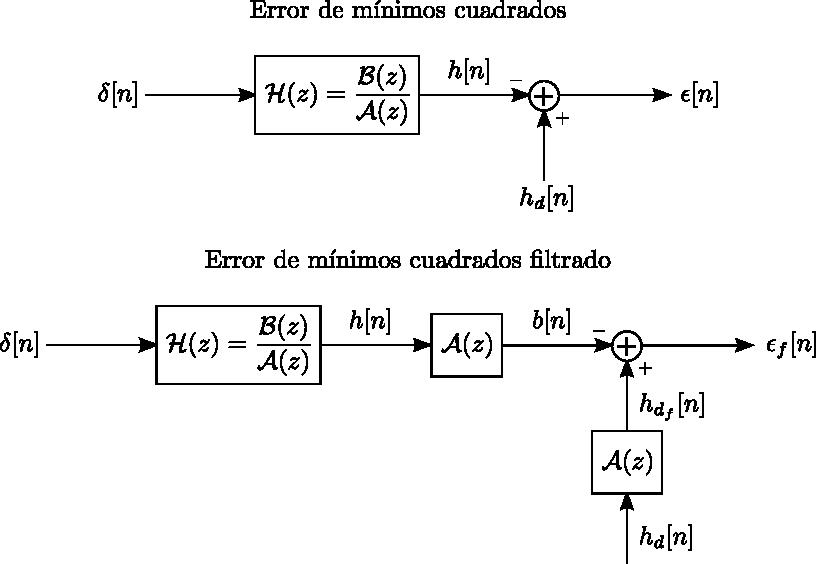
\includegraphics[width=\textwidth]{figuras/example_8_11_esquema.pdf}
  \end{minipage}\hfill
  \begin{minipage}[c]{0.2\textwidth}
    \caption{Conversión del problema LS no lineal a lineal para el diseño de un filtro.
    } \label{fig:example_8_11_esquema}
  \end{minipage}
\end{figure}
Por lo tanto, se minimiza el error LS filtrado
\[
 J_f=\sum_{n=0}^{N-1}(h_d[n]-b[n])^2
\]
donde \(h_{d_f}[n]\) está dado por 
\[
 h_{d_f}[n]=\sum_{k=0}^{p}a[k]h_d[n-k]
\]
con \(a[0]=1\). El error LS filtrado es por lo tanto
\begin{align*}
 J_f&=\sum_{n=0}^{N-1}\left(\sum_{k=0}^{p}a[k]hd[n-k]-b[n]\right)^2\\
  &\overset{(a)}{=}\sum_{n=0}^{N-1}\left(h_d[n]+\sum_{k=1}^{p}a[k]h_d[n-k]-b[n]\right)^2\\
  &=\sum_{n=0}^{N-1}\left[h_d[n]-\left(-\sum_{k=1}^{p}a[k]h_d[n-k]+b[n]\right)\right]^2,
\end{align*}
donde en \((a)\) se separó el sumando correspondiente a \(k=0\) de la sumatoria en \(k\). Para obtener los coeficientes del filtro que minimizan \(J_f\), se observa que los coeficientes \(b[n]\) solo aparecen en los primeros \((q+1)\) términos, ya que \(b[n]=0\) en \(n>q\). Como resultado, se tiene que
\[
 J_f(\abf,\,\bbf)=\sum_{n=0}^{q}\left[h_d[n]-\left(-\sum_{k=1}^{p}a[k]h_d[n-k]+b[n]\right)\right]^2+\sum_{n=q+1}^{N-1}\left[h_d[n]-\left(-\sum_{k=1}^{p}a[k]h_d[n-k]\right)\right]^2,
\]
donde \(\abf=[a[1]\,\dots\,a[p]]^T\) y \(\bbf=[b[0]\,\dots\,b[q]]^T\).
La primera sumatoria puede minimizarse, en realidad, anularse, haciendo que
\[
 h_d[n]-\left(-\sum_{k=1}^{p}a[k]h_d[n-k]+b[n]\right)=0,\qquad n=0,\,\dots,\,q,
\]
ya que \(h_d[n]\) puede elegirse de forma de anular la expresión para cada \(n\). Despejando \(b[n]\) se obtiene que
\[
 b[n]=h_d[n]+\sum_{k=1}^{p}a[k]h_d[n-k],\qquad n=0,\,\dots,\,q.
\]
Observando que
\begin{align*}
 b[0]&=h_d[0]\\
 b[1]&=h_d[1]+a[1]h_d[0]\\
 b[2]&=h_d[2]+a[1]h_d[1]+a[2]h_d[0]\\
 \vdots\;\;&\\
 b[q]&=h_d[q]+a[1]h_d[q-1]+\dots+a[p]h_d[q-p],
\end{align*}
en notación matricial, el LSE de los coeficientes de numerador es
\[
 \hat{\bbf}=\h+\Hbf_0\hat{\abf}
\]
donde
\[
 \h=
 \begin{bmatrix}
  h_d[0] & h_d[1] & \dots & h_d[q]
 \end{bmatrix}^T
 \qquad\qquad\textrm{y}\qquad\qquad
 \Hbf_0=
 \begin{bmatrix}
  0 & 0 & \dots & 0\\
  h_d[0] & 0 & \dots & 0\\
  h_d[1] & h_d[0] & \dots & 0\\
  \vdots & \vdots & \ddots &  \vdots\\
  h_d[p-1] & h_d[p-2] & \dots & h_d[0]\\
  \vdots & \vdots &  &  \vdots\\
  h_d[q-1] & h_d[q-2] & \dots & h_d[q-p]\\
 \end{bmatrix}.
\]
El vector \(\h\) tiene dimensiones \((q+1)\times1\), mientras que la matriz \(\Hbf_0\) tiene dimensiones \((q+1)\times p\) y es Toeplitz con la primera columna \([0,\,h_d[0],\,h_d[1],\,\dots,\,h_d[q-1]]^T\) y la primera fila \([0,\,\dots,\,0]\) asumiendo que \(q\geq p\).
Para encontrar el LSE de los coeficientes \(\abf\) del denominador hay que minimizar
\begin{align*}
 J_f(\abf,\,\hat{\bbf})&=\sum_{n=q+1}^{N-1}\left[h_d[n]-\left(-\sum_{k=1}^{p}a[k]h_d[n-k]\right)\right]^2\\
  &=(\x-\Hbf\thetabf)^T(\x-\Hbf\thetabf),
\end{align*}
donde \(\thetabf=\abf\) y
\[
 \x=
 \begin{bmatrix}
  h_d[q+1] & h_d[q+2] & \dots & h_d[N-1]
 \end{bmatrix}
 \quad\textrm{y}\quad
 \Hbf=
 \begin{bmatrix}
  h_d[q] & h_d[q-1] & \dots & h_d[q-p+1]\\
  h_d[q+1] & h_d[q] & \dots & h_d[q-p+2]\\
  \vdots & \vdots & & \vdots\\
  h_d[N-2] & h_d[N-3] & \dots & h_d[N-1-p]
 \end{bmatrix}.
\]
El vector \(\x\) tiene dimensiones \((N-1-q)\times1\) y \(\Hbf\) tiene dimensiones \((N-1-q)\times p\) y es Toeplitz con la primera columna \([h_d[q],\,h_d[q+1],\,\dots,\,h_d[N-2]]^T\) y la primera fila \([h_d[q],\,h_d[q-1],\,\dots,\,h_d[q-p+1]]\). Por lo tanto, el LSE de los coeficientes del denominador es
\[
 \hat{\abf}=(\Hbf^T\Hbf)^{-1}\Hbf^T\x.
\]
Este método para el diseño de filtros digitales se llama \emph{método de mínimos cuadrados de Prony}. Como ejemplo, se considera el diseño de un filtro pasabajos cuya respuesta en frecuencia ideal es
\[
 H_d'(f)=\left\{ 
 \begin{array}{ll}
  1 & |f|<f_c\\
  0 & |f|>f_c,
 \end{array}\right.
\]
donde \(f_c\) es la frecuencia de corte. La correspondiente respuesta al impulso es
\[
 h_d'[n]=\frac{\sin2\pi f_cn}{\pi n},\qquad-\infty<n<\infty
\]
la cual es infinita y no causal. Para asegurar causalidad, se trunca manteniendo solamente las muestras \(|n|\leq n_0\) y se retarda \(n_0\) muestras. Luego, para aproximar la respuesta al impulso deseada con el método LS de Prony, se asume que se dispone de \(N\) muestras de la respuesta al impulso
\begin{equation}\label{eq:ls_example_digital_filter_design_hd}
 h_d[n]=\frac{\sin2\pi f_c(n-n_0)}{\pi(n-n_0)},\qquad n-0,\,\dots,N-1.
\end{equation}
Se realizó una simulación por computadora empleando una señal deseada con frecuencia de corte \(f_c=0.1\), largo de \(N=51\) muestras y retardo de \(n_0=25\) muestras. Usando el método LS de Prony con \(p=q=10\) se diseñó un filtro digital con el objetivo de igualar su respuesta al impulso con la respuesta al impulso deseada. El resultado se muestra en la figura \ref{fig:example_8_11}.
\begin{figure}[!htb]
\begin{center}
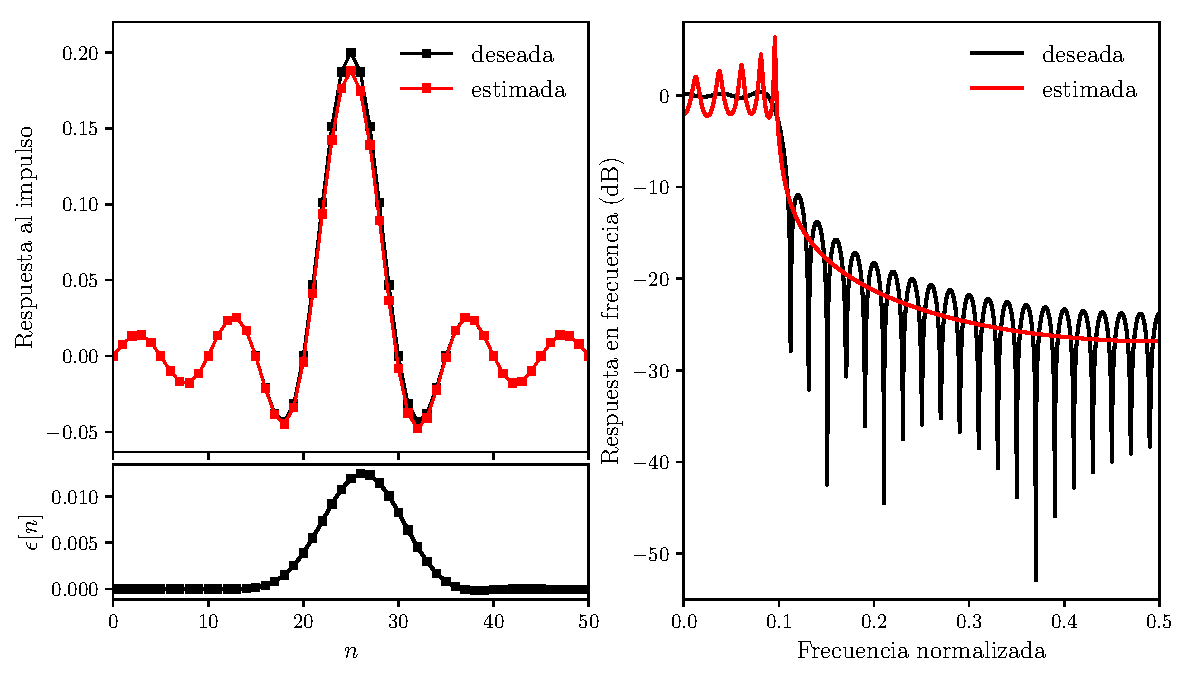
\includegraphics[width=\textwidth]{figuras/example_8_11.pdf}
\caption{\label{fig:example_8_11} Diseño de un filtro digital empleando el método de LS de Prony. Se compara la respuesta al impulso deseada y la obtenida \(h_d[n]\) y \(h[n]\) respectivamente, y las correspondientes respuestas en frecuencia \(H_d(f)\) y \(H(f)\). También se grafica el error de estimación \(\epsilon[n]=h_d[n]-h[n]\). Los parámetros empleados son \(p=q=10\), \(N=51\) muestras y \(f_c=0.1\).} 
\end{center}
\end{figure}
Respecto al filtro deseado, se observa que el efecto del truncamiento de la respuesta al impulso ideal se manifiesta en la estructura de lóbulos laterales en la respuesta en frecuencia deseada. La respuesta en frecuencia del filtro digital obtenido con el método de Prony tiene picos en la banda pasante y roll-off mas suave sin lóbulos laterales en comparación con la respuesta en frecuencia deseada. La aproximación al filtro deseado mejora si se incrementan los valores de \(p\) y \(q\). En la figura \ref{fig:example_8_11_pronys_method_python} se muestra el código en el lenguaje Python para el cálculo de los coeficientes \(\hat{\abf}\) y \(\hat{\bbf}\).
\begin{figure}[!htb]
\begin{center}
\lstinputlisting{figuras/example_8_11_pronys_method.py}
\caption{\label{fig:example_8_11_pronys_method_python} Implementación en el lenguaje Python del método LS de Prony para el diseño de filtros digitales.}
\end{center}
\end{figure}                                                                                                                                                                                                                                                                                                                                                                                                                                                                                                                                                                                                                                                                                                                                                                                                                                                                                                                                                                                                                                                                                                                                                                           
Para los parámetros elegidos en esta simulación, la matriz \(\Hbf^T\Hbf\) en el cálculo de \(\hat{\abf}\) está mal condicionada, y la inversión numérica produce un solución con errores numéricos intolerables. Una forma de regularizar la matriz es sumarle una matriz diagonal \(\varepsilon\I\) con \(\varepsilon\) pequeño. Está técnica se denomina \emph{regularización de Tikhonov}\footnote{Ver \url{https://en.wikipedia.org/wiki/Tikhonov_regularization}.}.

\subsection{Ejemplo: estimación de los parámetros AR de un modelo ARMA}\label{sec:ls_example_ar_parameters_arma_model}

A continuación se describe un método para la estimación de los parámetros AR de un modelo autorregresivo de media móvil (\emph{autoregressive–moving-average}, ARMA). Un modelo ARMA de un proceso WSS asume que la PSD es (por por ejemplo el capítulo 3 de \cite{hayes96statistical})
\[
 P_{xx}(f)=\frac{\sigma_u^2|B(f)|^2}{|A(f)|^2}
\]
donde
\[
 B(f)=1+\sum_{k=1}^{q}b[k]e^{-j2\pi fk}\qquad\qquad\textrm{y}\qquad\qquad A(f)=1+\sum_{k=1}^{p}a[k]e^{-j2\pi fk}.
\]
Los coeficientes \(b[k]\) se llaman parámetros MA del filtro, los coeficientes \(a[k]\) se llaman parámetros AR del filtro y \(\sigma_u^2\) es la varianza del ruido blanco conductor. El proceso se obtiene alimentando un filtro causal de respuesta de frecuencia \(B(f)/A(f)\) con ruido blanco de varianza \(\sigma_u^2\). Si los \(b[k]\) son nulos, se obtiene el proceso AR presentado en el ejemplo de la sección \ref{sec:ar_parameters_estimation}. La estimación de los parámetros AR de un modelo AR empleando el MLE asintótico fue discutido en el ejemplo de la sección \ref{sec:mle_ar_parameters_estimation}. En el caso de un proceso ARMA, no es posible calcular el MLE asintótico. Un enfoque alternativo se basa en el \emph{modelado de error de ecuación} de la ACF, en el cual se calculan los coeficientes AR, mientras que los coeficientes MA y la varianza del ruido se estiman con alguna otra técnica.

Para determinar la ACF, se parte de la transformada \(z\) de la PSD del modelo es (ver el capítulo 3 de \cite{hayes96statistical})
\[
 \mathcal{P}_{xx}(z)=\frac{\sigma_u^2\mathcal{B}(z)\mathcal{B}(z^{-1})}{\mathcal{A}(z)\mathcal{A}(z^{-1})}
\]
donde \(B(f)=\mathcal{B}(e^{j2\pi f})\), \(A(f)=\mathcal{A}(e^{j2\pi f})\). Se deducirá una ecuación en diferencias para la ACF, que será la base del enfoque de modelado de error de ecuación. Tomando la transformada \(z\) inversa de \(\mathcal{A}(z)\mathcal{P}_{xx}(z)\), se tiene que
\[
 \mathcal{Z}^{-1}\{\mathcal{A}(z)\mathcal{P}_{xx}(z)\}=\mathcal{Z}^{-1}\left\{\sigma_u^2\mathcal{B}(z)\frac{\mathcal{B}(z^{-1})}{\mathcal{A}(z^{-1})}\right\}.
\]
Considerando que
\[
 h[n]=\mathcal{Z}^{-1}\left\{\frac{\mathcal{B}(z^{1})}{\mathcal{A}(z^{1})}\right\},
\]
por la propiedad de inversión temporal de la transformada \(z\), que indica que
\[
 h[n]\overset{\mathcal{Z}}{\longleftrightarrow}\mathcal{H}(z)\qquad\qquad\Rightarrow\qquad\qquad h[-n]\overset{\mathcal{Z}}{\longleftrightarrow}\mathcal{H}(z^{-1}),
\]
se obtiene que
\begin{align*}
 \mathcal{Z}^{-1}\left\{\sigma_u^2\mathcal{B}(z)\frac{\mathcal{B}(z^{-1})}{\mathcal{A}(z^{-1})}\right\}
 &=\sigma_u^2b[n]*h[-n]\\
 &=\sigma_u^2\sum_{k=-\infty}^{\infty}b[k]h[k-n]\\
 &=\sigma_u^2\sum_{k=0}^{q}b[k]h[k-n]\\
 &=\sigma_u^2(b[0]h[-n]+\dots+b[q]h[q-n])\\
 &=0\qquad\textrm{si }q-n<0,
\end{align*}
donde en la última igualdad se consideró que \(h[n]\) es causal y por lo tanto, \(h[n]=0\) si \(n<0\). Por lo tanto
\[
 \mathcal{Z}^{-1}\{\mathcal{A}(z)\mathcal{P}_{xx}(z)\}=0\qquad\textrm{si }n>q,
\]
y teniendo en cuenta que la secuencia es la convolución entre \(a[n]\) y \(r_{xx}[n]\), se obtiene que
\begin{equation}\label{eq:modified_yule_walker}
 \sum_{k=0}^{p}a[k]r_{xx}[n-k]=0\qquad\textrm{si }n>q.
\end{equation}
con \(a[0]=1\). Estas ecuaciones se denominan \emph{ecuaciones de Yule-Walker modificadas}. Notar del ejemplo de la sección \ref{sec:mle_ar_parameters_estimation} que las ecuaciones de Yule-Walker son idénticas excepto que se cumplen para \(n>0\), ya que \(q=0\) en un proceso AR.

En la práctica, la ACF se estima como
\[
 \hat{r}_{xx}[k]=\frac{1}{N}\sum_{n=0}^{N-1-|k|}x[n]x[n+|k|]
\]
asumiendo que \(x[n]\) se conoce en \(n=0,\,\dots,\,N-1\). Sustituyendo en la ecuación \ref{eq:modified_yule_walker}, se obtiene que
\[
 \sum_{k=0}^{p}a[k]\hat{r}_{xx}[n-k]=\epsilon[n]\qquad n>q,
\]
donde \(\epsilon[n]\) denota el error en la estimación de la ACF con la ACF muestral. El modelo queda
\[
 \hat{r}_{xx}[n]=-\sum_{k=1}^{p}a[k]\hat{r}_{xx}[n-k]+\epsilon[n]\qquad n>q,
\]
el cual es lineal con los parámetros AR desconocidos. Si la ACF es estimada en los retardos \(n=0,\,\dots,\,M\), con \(M\leq N-1\), el LSE de \(a[k]\) minimiza
\begin{align*}
 J&=\sum_{n=q+1}^M\left[\hat{r}_{xx}[n]-\left(-\sum_{k=1}^{p}a[k]\hat{r}_{xx}[n-k]\right)\right]^2\\
  &=(\x-\Hbf\thetabf)^T(\x-\Hbf\thetabf),
\end{align*}
con
\[
 \x=
 \begin{bmatrix}
  \hat{r}_{xx}[q+1]\\ \hat{r}_{xx}[q+2]\\ \vdots\\ \hat{r}_{xx}[M]     
 \end{bmatrix}
 \qquad\qquad
 \thetabf=
 \begin{bmatrix}
  a[1]\\ a[2]\\ \vdots\\ a[p]     
 \end{bmatrix}
 \qquad\qquad
 \Hbf=
 \begin{bmatrix}
  \hat{r}_{xx}[q] & \hat{r}_{xx}[q-1] & \dots & \hat{r}_{xx}[q-p+1]\\
  \hat{r}_{xx}[q+1] & \hat{r}_{xx}[q] & \dots & \hat{r}_{xx}[q-p+2]\\
  \vdots & \vdots & & \vdots\\
  \hat{r}_{xx}[M-1] & \hat{r}_{xx}[M-2] & \dots & \hat{r}_{xx}[M-p]
 \end{bmatrix}.
\]
El LSE de \(\thetabf\) es \((\Hbf^T\Hbf)^{-1}\Hbf^T\x\) y se llama \emph{ecuaciones por mínimos cuadrados de Yule-Walker modificadas}.

\subsection{Ejemplo: cancelador de ruido adaptativo}

Un problema común en procesamiento de señales es la reducción de ruido, como por ejemplo, la supresión de la interferencia de 50 Hz de la red eléctrica en un circuito eléctrico. Una forma de hacerlo es mediante un cancelador de ruido adaptativo. Se asume que se dispone de una señal de ruido de referencia que luego de ser filtrada adecuadamente, puede igualarse al ruido y cancelarlo mediante la resta. Por ejemplo, para cancelar el ruido de 50 Hz se necesita conocer la amplitud y la fase, pero en general son desconocidas. En este caso, el objetivo del filtrado es igualar la amplitud y la fase del ruido de interferencia.  
\begin{figure}[!htb]
  \begin{minipage}[c]{0.5\textwidth}
    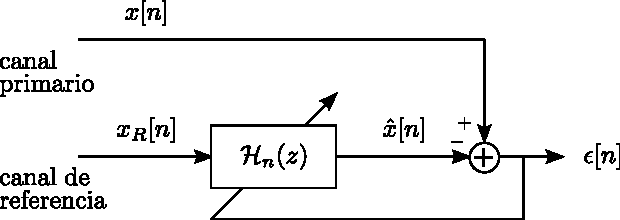
\includegraphics[width=\textwidth]{figuras/example_8_13_cancelador.pdf}
  \end{minipage}\hfill
  \begin{minipage}[c]{0.4\textwidth}
    \caption{
       Esquema del cancelador de ruido adaptativo en tiempo discreto.
    } \label{fig:example_8_13_cancelador}
  \end{minipage}
\end{figure}
En la figura \ref{fig:example_8_13_cancelador} se muestra un esquema del cancelador. El canal primario contiene el ruido \(x[n]\) a ser cancelado. El canal de referencia contiene una secuencia conocida \(x_R[n]\) que es similar pero no igual al ruido. Para realizar la cancelación, el ruido de referencia es filtrado con el objetivo de igualar el ruido a cancelar. Los coeficientes del filtro \(\mathcal{H}_n(z)\) se determinan en cada instante \(n\) de forma de que \(\hat{x}[k]\approx x[k]\) para \(k=0,\,1,\,\dots,\,n\). Como se busca que \(\epsilon[n]\approx0\), los coeficientes del filtro en el instante \(n\) se eligen de forma de minimizar
\begin{align*}
 J&=\sum_{k=0}^{n}\epsilon[n]\\
  &=\sum_{k=0}^{n}(x[k]-\hat{x}[n])\\
  &=\sum_{k=0}^{n}\left(x[k]-\sum_{l=0}^{p-1}h_n[l]x_R[k-l]\right)^2
\end{align*}
donde \(h_n[l]\) son los coeficientes del filtro en el tiempo \(n\). Se reconoce que la estimación de los coeficientes puede resolverse como un problema de LS secuencial (ver la sección \ref{sec:ls_sequential}). Hay que observar que el problema de LSE asume que la interferencia es estacionaria. En caso contrario, el filtro debería cambiar sus coeficientes rápidamente para responder al cambio en la interferencia. La velocidad de respuesta al cambio depende de la cantidad de términos incluidos en \(J[n]\). Si la interferencia sufre un cambio abrupto en el tiempo \(n=n_0\), se espera que los coeficientes sean erroneos hasta \(n\gg n_0\). Para permitir que el filtro se adapte mas rápidamente a los cambios se puede ponderar mas fuertemente los errores mas recientes en \(J[n]\) introduciendo un factor de ponderación o \emph{factor de olvido} \(\lambda\), con \(0<\lambda<1\), como sigue
\[
 J[n]=\sum_{k=0}^{n}\lambda^{n-k}\left(x[k]-\sum_{l=0}^{p-1}h_n[l]x_R[k-l]\right)^2.
\]
Esta modificación desestima exponencialmente los errores previos, permitiendo que el filtro reaccione mas rápidamente a los cambios. En contrapartida, las estimaciones son mas ruidosas por tomar en cuenta efectivamente menos errores LS. Notar que la solución no cambia si se minimiza
\[
 J[n]=\sum_{k=0}^{n}\frac{1}{\lambda^k}\left(x[k]-\sum_{l=0}^{p-1}h_n[l]x_R[k-l]\right)^2
\]
para cada \(n\), ya que \(\lambda^n\) es una constante multiplicativa de \(J[n]\) para cada \(n\). De esta forma, el problema es el LS secuencia ponderado descripto en la sección \ref{sec:ls_sequential}. En este caso, el modelo de la señal en el tiempo \(n\) es
\[
\underbrace{\vphantom{\begin{bmatrix}0\\0\\\vdots\\x_R[0]\\\vdots\\x_R[n-p+1]\end{bmatrix}}
 \begin{bmatrix}
  x[0]\\ x[1]\\ \vdots \\ x[n]
 \end{bmatrix}}_{\displaystyle \x[n]}
 =
 \underbrace{
 \begin{bmatrix}
  x_R[0] & 0 & \dots & 0\\
  x_R[1] & x_R[0] & \dots & 0\\
  \vdots & \vdots &  & \vdots\\
  x_R[p-1] & x_R[p-2] & \dots & x_R[0]\\
  \vdots & \vdots &  & \vdots\\
  x_R[n] & x_R[n-1] & \dots & x_R[n-p+1]\\
 \end{bmatrix}}_{\displaystyle \Hbf[n]}
 \underbrace{\vphantom{\begin{bmatrix}0\\0\\\vdots\\x_R[0]\\\vdots\\x_R[n-p+1]\end{bmatrix}}
 \begin{bmatrix}
  h_n[0]\\h_n[1]\\\vdots\\h_n[p-1]
 \end{bmatrix}}_{\displaystyle \thetabf[n]}
\]
y \(\C[n]=\operatorname{diag}(1,\,\lambda,\,\dots,\,\lambda^n)\), y se quiere minimizar
\[
 J[n]=(\x[n]-\Hbf[n]\thetabf[n])^T\C^{-1}[n](\x[n]-\Hbf[n]\thetabf[n])
\]
para cada \(n\). De las ecuaciones \ref{eq:ls_sequential_estimator_update}-\ref{eq:ls_sequential_covariance_update} del LSE secuencial con 
\begin{align*}
 \hat{\thetabf}[n]&=
 \begin{bmatrix}
  h_n[0] & h_n[1]& \dots & h_n[p-1]
 \end{bmatrix}^T,\\
 \h[n]&=
 \begin{bmatrix}
  x_R[n] & x_R[n-1] & \dots & x_R[n-p+1]
 \end{bmatrix}^T
\end{align*}
y los pesos \(\sigma_n^2=\lambda^n\), las ecuaciones del algoritmo resultan en
\[
 \hat{\thetabf}[n]=\hat{\thetabf}[n-1]+\K[n]e[n]
\]
donde
\[
\begingroup
 \renewcommand*{\arraystretch}{2.0}
\begin{array}{ccl}
 e[n]&=&x[n]-\h^T[n]\hat{\thetabf}[n-1]\\
 \h[n]&=&[x_R[n]\; x_R[n-1]\; \dots \; x_R[n-p+1]]^T\\
 \K[n]&=&\displaystyle\frac{\bm{\Sigma}[n-1]\h[n]}{\lambda^n+\h^T[n]\bm{\Sigma}[n-1]\h[n]}\\
 \bm{\Sigma}[n]&=&(\I-\K[n]\h^T[n])\bm{\Sigma}[n-1].
\end{array}
\endgroup
\]
Observar que \(e[n]=x[n]-\h^T[n]\hat{\thetabf}[n-1]\) en el algoritmo no es el error de estimación en el paso \(n\), que está dado por \(e[n]=x[n]-\hat{x}[n]=x[n]-\h^T[n]\hat{\thetabf}[n]\), si no que es el error de estimación en el paso \(n\) considerando los coeficientes del filtro calculados en el paso \(n-1\). El factor de olvido tiene que cumplir \(0<\lambda<1\), y típicamente se elige cercano a 1. En la figura \ref{fig:example_8_13_v2_code} se muestra la implementación en el lenguaje Python del algoritmo.

A continuación se muestra el resultado de una simulación por computadora. La interferencia es la señal sinusoidal
\[
 x[n]=A[n]\cos(2\pi(0.1)n+\pi/4),\qquad\qquad\textrm{con}\qquad\qquad
 A[n]=\left\{ 
 \begin{array}{ll}
  12, & 0\leq n\leq N/2\\
  4, & N/2+1\leq n\leq N-1,
 \end{array}\right.
\]
con \(N=100\). Notar que tiene un cambio abrupto de amplitud. La señal de referencia es
\[
 x_R[n]=\cos(2\pi(0.1)n),
\]
y se implementó un cancelador de ruido con dos coeficientes (\(p=2\)) ya que solo tiene que modificar a la señal de referencia en amplitud y fase para hacer que coincida con la interferencia. Para la inicialización del LSE secuencial se eligió
\[
 \hat{\thetabf}[-1]=0,\qquad\qquad
 \bm{\Sigma}[-1]=10^5\I
\]
y un factor de olvido \(\lambda=0.9\). La varianza del estimador en la matriz de covarianza inicial es grande para darle poca confianza al estimador inicial, que fue elegido de forma arbitraria. El factor de olvido es relativamente bajo (olvido rápido) para que el filtro pueda adaptarse rápidamente al cambio en la interferencia. 
En la figura \ref{fig:example_8_13} se muestra el resultado.
\begin{figure}[!htb]
\begin{center}
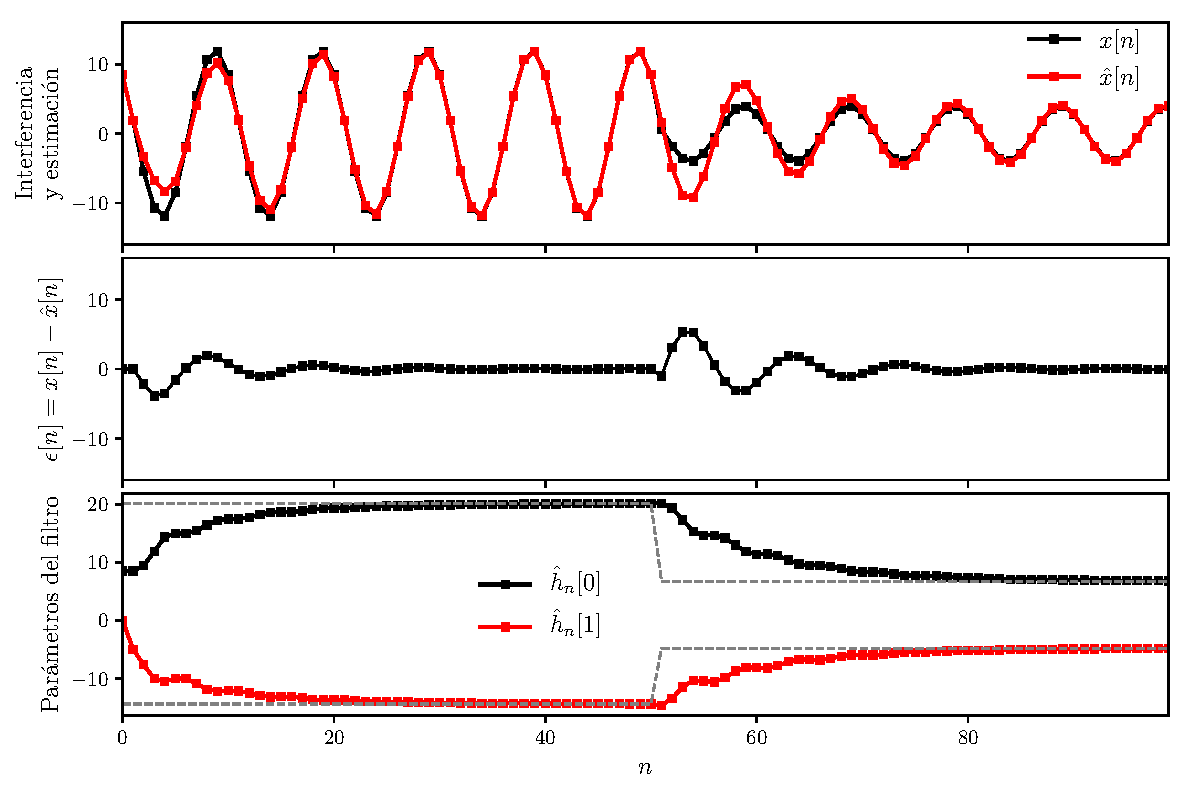
\includegraphics[width=1\textwidth]{figuras/example_8_13.pdf}
\caption{\label{fig:example_8_13} Cancelador de ruido. Se muestra la interferencia y la señal estimada a partir de la referencia, el error de estimación y los coeficientes del filtro del cancelador estimados. También se grafica los coeficientes del filtro ideal del cancelador.}
\end{center}
\end{figure}
Se observa que la interferencia es cancelada relativamente rápido. Como el factor de olvido es bajo, la señal estimada \(\hat{x}[n]\) se adapta relativamente rápido al cambio en la interferencia. También se observa que los coeficientes del filtro adaptativo convergen a los valores ideales. Para calcular los valores ideales de los coeficientes del filtro del cancelador, se considera que si la entrada a un filtro es \(e^{j\omega n}\), la salida es \(\mathcal{H}(e^{j\omega})e^{j\omega n}\), y como en este caso se requiere que si la entrada es la referencia \(x_R[n]=e^{j\pi n/5}\) la salida sea la interferencia \(x[n]=a[n]e^{j\pi/4}e^{j\pi n/5}\), los coeficientes del filtro ideal cumplen que
\[
 \mathcal{H}(e^{j\pi/10})=h[0]+h[1]e^{-j\pi/10}=a[n]e^{j\pi/4}.
\]
Aplicando la fórmula de Euler, igualando la parte real e imaginaria a ambos lados de la igualdad y resolviendo el sistema de dos ecuaciones y dos incógnitas se llega a que
\[
 h[0]=A[n]\frac{\sin9\pi/20}{\sin\pi/5}\qquad\qquad\textrm{y}\qquad\qquad
 h[1]=-A[n]\frac{\sin\pi/4}{\sin\pi/5}.
\]
En la figura \ref{fig:example_8_13_v2_code} se muestra la parte principal del código en Python del cancelador.
\begin{figure}[!htb]
\begin{center}
\lstinputlisting{figuras/example_8_13_v2_code.py}
\caption{\label{fig:example_8_13_v2_code} Implementación del cancelador en el lenguaje Python.}
\end{center}
\end{figure}  

\section{Problemas}

\subsection{Problema 1}\label{sec:problem_8_1}

Se quiere minimizar el error LS
\[
 J=\sum_{n=0}^{N-1}(x[n]-A\cos2\pi f_0n-Br^n)^2
\]
para encontrar el LSE de \(\thetabf=[A\,f_0\,B\,r]^T\), donde \(0<r<1\). ¿Se trata de un problema LS lineal o no lineal? ¿Es el error LS cuadrático en alguno de los parámetros? En caso afirmativo, ¿en cuales? ¿Cómo se puede resolver este problema de minimización empleando una computadora?

\paragraph{Solución} Claramente es un problema LS no lineal debido a los parámetros \(f_0\) y \(r\). Sin embargo, es un problema LS lineal en los parámetros \(A\) y \(B\), y por lo tanto se puede reducir su complejidad empleando la técnica de separación de parámetros como se explica a continuación. El modelo de la señal se puede expresar como
\[
 \s=\Hbf(\alphabf)\bm{\beta},
\]
donde el vector \(\alphabf\) contiene el conjunto de parámetros no lineales y \(\bm{\beta}\) contiene el conjunto de parámetros lineales en el modelo. En este caso, el modelo de señal es
\[
 s[n]=A\cos2\pi f_0n-Br^n,\qquad n=0,\,\dots,\,N-1,
\]
y separando los parámetros puede expresarse en notación matricial como
\[
 \s=
 \begin{bmatrix}
  1 & 1\\
  \cos2\pi f_0 & r\\
  \cos4\pi f_0 & r^2\\
  \vdots & \vdots\\
  \cos2\pi f_0(N-1) & r^{N-1}
 \end{bmatrix}
 \begin{bmatrix}
  A\\B
 \end{bmatrix}.
\]
Por lo tanto,
\[
 \alphabf=
 \begin{bmatrix}
  f_0\\ r
 \end{bmatrix},\qquad\qquad
 \bm{\beta}=
 \begin{bmatrix}
  A\\ B
 \end{bmatrix},\qquad\qquad
 \Hbf(\alphabf)=
 \begin{bmatrix}
  1 & 1\\
  \cos2\pi f_0 & r\\
  \cos4\pi f_0 & r^2\\
  \vdots & \vdots\\
  \cos2\pi f_0(N-1) & r^{N-1}
 \end{bmatrix}.
\]
Como
\[
 J(\alphabf,\,\bm{\beta})=(\x-\Hbf(\alphabf)\bm{\beta})^T(\x-\Hbf(\alphabf)\bm{\beta}),
\]
el valor de \(\bm{\beta}\) que minimiza \(J\) para un valor de \(\alphabf\) dado es el LSE lineal usual,
\begin{equation}\label{eq:problem_8_1_beta_lse}
 \hat{\bm{\beta}}=(\Hbf^T(\alphabf)\Hbf(\alphabf))^{-1}\Hbf(\alphabf)\x
\end{equation}
y de la ecuación \ref{eq:ls_lls_min_error_vector}, el error LS mínimo es
\[
 J(\alphabf,\,\bm{\beta})=\x^T\left[\I-\Hbf(\alphabf)(\Hbf^T(\alphabf)\Hbf(\alphabf))^{-1}\Hbf(\alphabf)\right]\x,
\]
y depende únicamente de \(\alphabf\). Por lo tanto, para calcular el LSE de \(\alphabf\) hay que maximizar
\[
 \x^T\Hbf(\alphabf)(\Hbf^T(\alphabf)\Hbf(\alphabf))^{-1}\Hbf(\alphabf)\x.
\]
La maximización puede hacerse mediante una búsqueda de grilla en \(0\leq f_0\leq0.5\) y \(0< r<1\). Resolviendo la ecuación \ref{eq:problem_8_1_beta_lse} con \(\alphabf=\hat{\alphabf}=[\hat{f}_0\,\hat{r}]\) donde \(\hat{f}_0\) y \(\hat{r}\) son los valores obtenidos en la maximización, se obtiene \(\hat{A}\) y \(\hat{B}\).



\subsection{Problema 2}\label{sec:problem_8_2}

Mostrar que se cumple la desigualdad indicada en la ecuación \ref{eq:ls_lls_min_error_bounds}.

\paragraph{Solución} De la ecuación \ref{eq:ls_lls_criterion_scalar} se deduce que \(J(\theta)\geq0\) por lo que \(J_\textrm{mín}\geq0\). Además, de la ecuación \ref{eq:ls_lls_min_error_scalar} se observa que \(J_\textrm{mín}\leq\sum_{n=0}^{N-1}x^2[n]\), concluyendo que 
\[
 0\leq J_\textrm{mín}\leq \sum_{n=0}^{N-1}x^2[n].
\]

\subsection{Problema 3}

Para el modelo de señal
\[
 s[n]=\left\{ 
 \begin{array}{cc}
  A & 0\leq n\leq M-1\\
  -A & M\leq n\leq N-1,
 \end{array}\right.
\]
encontrar el LSE de \(A\) y el error LS mínimo. Asumir que se observa \(x[n]=s[n]+w[n]\) para \(n=0,\,\dots,\,N-1\). Si ahora \(w[n]\) es WGN con varianza \(\sigma^2\), encontrar la PDF del LSE.

\paragraph{Solución} De la ecuación \ref{eq:ls_lls_estimator_scalar}, el LSE es
\[
 \hat{A}=\frac{\displaystyle
 \sum_{n=0}^{N-1}x[n]h[n]}{\displaystyle\sum_{n=0}^{N-1}h^2[n]}.
\]
El modelo de la señal es
\[
 s[n]=Ah[n],\qquad\qquad\textrm{con}\qquad\qquad
 h[n]=\left\{ 
 \begin{array}{cc}
  1 & 0\leq n\leq M-1\\
  -1 & M\leq n\leq N-1,
 \end{array}\right.
\]
por lo que el LSE es
\[
 \hat{A}=\frac{\displaystyle\sum_{n=0}^{M-1}x[n]-\sum_{n=M}^{N-1}x[n]}{N}.
\]
De la ecuación \ref{eq:ls_lls_min_error_scalar}
\[
 J_\textrm{mín}=\sum_{n=0}^{N-1}x^2[n]-\frac{\left(\displaystyle
 \sum_{n=0}^{N-1}x[n]h[n]\right)^2}{\displaystyle\sum_{n=0}^{N-1}h^2[n]},
\]
resultando en
\[
 J_\textrm{mín}=\sum_{n=0}^{N-1}x^2[n]-N\hat{A}.
\]
Si \(w[n]\) es WGN con varianza \(\sigma^2\), \(x[n]\sim\mathcal{N}(Ah[n],\,\sigma^2)\). Por lo tanto,
\begin{align*}
 E(\hat{A})&=\frac{\displaystyle \sum_{n=0}^{M-1}E(x[n])-\sum_{n=M}^{N-1}E(x[n])}{N}\\
   &=\frac{\displaystyle A\sum_{n=0}^{M-1}h[n]-A\sum_{n=M}^{N-1}h[n]}{N}\\
   &=\frac{AM-A(N-M)(-1)}{N}\\
   &=A,
\end{align*}
y
\begin{align*}
 \var(\hat{A})&\overset{(a)}{=}\frac{\displaystyle\sum_{n=0}^{M-1}\var(x[n])+\sum_{n=M}^{N-1}\var(x[n])}{N}\\
   &=\frac{\sigma^2M+\sigma^2(N-M)}{N^2}\\
   &=\frac{\sigma^2}{N},
\end{align*}
donde en \((a)\) se consideró que como las muestras \(w[n]\) son independientes también lo son las muestras \(x[n]\). Como \(\hat{A}\) es una combinación lineal de variables aleatorias gaussianas independientes, \(\hat{A}\) también es gaussiana, se concluye que
\[
 \hat{A}\sim\mathcal{N}\left(A,\,\frac{\sigma^2}{N}\right).
\]

\subsection{Problema 4}\label{sec:problem_8_4}

Deducir que el LSE de un parámetro vectorial está dado por la ecuación \ref{eq:ls_lls_estimator_vector} verificando que se cumple la identidad
\[
 J=(\x-\Hbf\hat{\thetabf})^T(\x-\Hbf\hat{\thetabf})+(\hat{\thetabf}-\thetabf)^T\Hbf^T\Hbf(\hat{\thetabf}-\thetabf),
\]
donde
\[
 \hat{\thetabf}=(\Hbf^T\Hbf)^{-1}\Hbf^T\x.
\]
Para completar la prueba, mostrar que \(J\) se minimiza cuando \(\hat{\thetabf}=\thetabf\), asumiendo que \(\Hbf\) es de rango completo por lo que \(\Hbf^T\Hbf\) es definida positiva.

\paragraph{Solución} Que la identidad se cumple fue probado en el problema de la sección \ref{sec:problem_5_19}. Para deducir que el error se minimiza cuando \(\hat{\thetabf}=\thetabf\), se observa que el primer sumando es una constante. Además, como \(\Hbf^T\Hbf\) es definida positiva, el segundo sumando es no-negativo. Esto implica que \(J\) es mínimo cuando el segundo sumando es nulo, lo que se da solo si \(\hat{\thetabf}=\thetabf\).

\subsection{Problema 5}

Para el modelo de señal
\[
 s[n]=\sum_{i=1}^pA_i\cos(2\pi f_in)
\]
donde las frecuencias \(f_i\) son conocidas y se quiere estimar las amplitudes \(A_i\), encontrar las ecuaciones normales del LSE (no intentar resolverlas). Luego, si las frecuencias son \(f_i=i/N\), encontrar explícitamente el LSE y el error LS mínimo. Finalmente, si \(x[n]=s[n]+w[n]\) donde \(w[n]\) es WGN de varianza \(\sigma^2\), determinar la PDF del LSE asumiendo las frecuencias indicadas. Sugerencia: las columnas de \(\Hbf\) son ortogonales para las frecuencias dadas.

\paragraph{Solución} El modelo de la señal en forma matricial es
\[
 \s=\Hbf\thetabf,\quad\textrm{con}\quad
 \Hbf=
 \begin{bmatrix}
  1 & 1 & \dots & 1\\
  \cos2\pi f_1 & \cos2\pi f_2 & \dots & \cos2\pi f_p\\
  \cos4\pi f_1 & \cos4\pi f_2 & \dots & \cos4\pi f_p\\
  \vdots & \vdots & & \vdots \\
  \cos2\pi f_1(N-1) & \cos2\pi f_2(N-1) & \dots & \cos2\pi f_p(N-1)\\
 \end{bmatrix}
 \quad\textrm{y}\quad
 \thetabf=
 \begin{bmatrix}
  A_1 \\ A_2 \\ \vdots \\ A_p
 \end{bmatrix}.
\]
Las ecuaciones normales son 
\[
 \Hbf^T\Hbf\thetabf=\Hbf^T\x.
\]
Si las frecuencias son \(f_i=i/N\) y \(\h_i\) es la columna \(i\)-ésima de \(\Hbf\), se cumple que
\[
 \h_i^T\h_j=\sum_{n=0}^{N-1}\cos\left(\frac{2\pi in}{N}\right)\cos\left(\frac{2\pi jn}{N}\right)=\frac{N}{2}\delta_{ij},
\]
como se mostró en el problema de la sección \ref{sec:problem_4_5} (ver también el ejemplo de la sección \ref{sec:linear_model_fourier_analysis}). Por lo tanto,
\[
 \Hbf^T\Hbf=\frac{N}{2}\I
\]
y el LSE es
\[
 \hat{\thetabf}=(\Hbf^T\Hbf)^{-1}\Hbf^T\x=\frac{2}{N}\Hbf^T\x.
\]
Además, como elemento \(i\)-ésimo de \(\Hbf^T\x\) es
\[
 [\Hbf^T\x]_i=\sum_{n=0}^{N-1}x[n]\cos\left(\frac{2\pi in}{N}\right),
\]
el elemento \(i\)-ésimo \(\thetabf_i\) del LSE es
\[
\hat{A}_i=\frac{2}{N}\sum_{n=0}^{N-1}x[n]\cos\left(\frac{2\pi in}{N}\right).
\]
De la ecuación \ref{eq:ls_lls_min_error_vector}, el error LS mínimo es 
\begin{align*}
 J_\textrm{mín}&=\x^T(\I-\Hbf(\Hbf^T\Hbf)^{-1}\Hbf^T)\x\\
  &=\x^T\x-\frac{2}{N}\x^T\Hbf\Hbf^T\x\\
  &\overset{(a)}{=}\x^T\x-\frac{N}{2}\hat{\thetabf}^T\hat{\thetabf},
\end{align*}
donde en \((a)\) se empleó que \(\Hbf^T\x=(N/2)\hat{\thetabf}\). Finalmente,
\[
 J_\textrm{mín}=\sum_{n=0}^{N-1}x^2[n]-\frac{N}{2}\sum_{i=1}^{p}\hat{A}_i^2.
\]
Si \(x[n]=s[n]+w[n]\) con \(w[n]\) WGN de varianza \(\sigma^2\), el LSE es el estimador MVU del modelo lineal y tiene las mismas propiedades, como la indicada en la sección \ref{sec:linear_model_extension}. La esperanza del estimador es
\begin{align*}
 E(\hat{\thetabf})=(\Hbf^T\Hbf)^{-1}\Hbf^TE(\x)=(\Hbf^T\Hbf)^{-1}\Hbf^T\s=(\Hbf^T\Hbf)^{-1}\Hbf^T\Hbf\thetabf=\thetabf,
\end{align*}
y a matriz de covarianza es
\begin{align*}
 \C_{\hat{\thetabf}}&=E\left\{[\hat{\thetabf}-E(\hat{\thetabf})][\hat{\thetabf}-E(\hat{\thetabf})]^T\right\}\\
   &=E\left\{[(\Hbf^T\Hbf)^{-1}\Hbf^T\x-\thetabf][(\Hbf^T\Hbf)^{-1}\Hbf^T\x-\thetabf]^T\right\}\\
   &=E\left[(\Hbf^T\Hbf)^{-1}\Hbf^T(\x-\Hbf\thetabf)(\x-\Hbf\thetabf)^T\Hbf(\Hbf^T\Hbf)^{-1}\right]\\
   &=(\Hbf^T\Hbf)^{-1}\Hbf^TE(\w\w^T)\Hbf(\Hbf^T\Hbf)^{-1}\\
   &=(\Hbf^T\Hbf)^{-1}\Hbf^T(\sigma^2\I)\Hbf(\Hbf^T\Hbf)^{-1}\\
   &=\sigma^2(\Hbf^T\Hbf)^{-1}
\end{align*}
resultando en
\[
 \C_{\hat{\thetabf}}=\frac{2\sigma^2}{N}\I.
\]
Finalmente, como \(\hat{\thetabf}\) es una combinación lineal de \(\x\) se concluye que
\[
 \hat{\thetabf}=\mathcal{N}\left(\thetabf,\,\frac{2\sigma^2}{N}\I\right).
\]

\subsection{Problema 6}

Para el LSE general dado por la ecuación \ref{eq:ls_lls_estimator_vector}, encontrar la PDF del LSE en el caso en que \(\x\sim\mathcal{N}(\Hbf\thetabf,\,\sigma^2\I)\). ¿El LSE es insesgado?

\paragraph{Solución} Como indica la ecuación \ref{eq:ls_lls_estimator_vector}, el LSE es
\[
 \hat{\thetabf}=(\Hbf^T\Hbf)^{-1}\Hbf^T\x.
\]
Por tratarse de una combinación lineal de variables aleatorias gaussianas independientes, tiene PDF gaussiana, y por lo tanto, queda caracterizada por la media y la matriz de covarianza. La esperanza es
\[
 E(\hat{\thetabf})=(\Hbf^T\Hbf)^{-1}\Hbf^TE(\x)=(\Hbf^T\Hbf)^{-1}\Hbf^T\Hbf\thetabf=\thetabf,
\]
indicando que el LSE es insesgado. La matriz de covarianza es
\[
 \C_{\hat{\thetabf}}=E\left\{[\hat{\thetabf}-E(\hat{\thetabf})][\hat{\thetabf}-E(\hat{\thetabf})]^T\right\}
\]
y teniendo en cuenta que
\begin{align*}
 \hat{\thetabf}-E(\hat{\thetabf})&=(\Hbf^T\Hbf)^{-1}\Hbf^T\x-\thetabf\\
  &=(\Hbf^T\Hbf)^{-1}(\Hbf^T\x-\Hbf^T\Hbf\thetabf)\\
  &=(\Hbf^T\Hbf)^{-1}\Hbf^T(\x-\Hbf\thetabf),
\end{align*}
la matriz de covarianza queda
\begin{align*}
 \C_{\hat{\thetabf}}&=(\Hbf^T\Hbf)^{-1}\Hbf^TE[(\x-\Hbf\thetabf)(\x-\Hbf\thetabf)^T]\Hbf(\Hbf^T\Hbf)^{-1}\\
  &=(\Hbf^T\Hbf)^{-1}\Hbf^T(\sigma^2\I)\Hbf(\Hbf^T\Hbf)^{-1}\\
  &=\sigma^2(\Hbf^T\Hbf)^{-1}.
\end{align*}
Se concluye que 
\[
 \hat{\thetabf}\sim\mathcal{N}(\thetabf,\,\sigma^2(\Hbf^T\Hbf)^{-1}).
\]

\subsection{Problema 7}

En este problema se considera la estimación de la varianza \(\sigma^2\) del ruido en el modelo \(\x=\Hbf\thetabf+\w\), donde \(\w\) es ruido de media nula y varianza con matriz de covarianza \(\sigma^2\I\). Se propone el estimador
\[
 \hat{\sigma^2}=\frac{1}{N}J_{\min}=\frac{1}{N}(\x-\Hbf\thetabf)^T(\x-\Hbf\thetabf),
\]
donde \(\hat{\thetabf}\) es el LSE de \(\thetabf\) dado por la ecuación \ref{eq:ls_lls_estimator_vector}. ¿Es este estimador insesgado? En caso de que no lo sea, proponer uno que sea insesgado. Explicar los resultados. Sugerencia: serán útiles las identidades \(E(\x^T\y)=E(\tr(\y\x^T))=\tr(E(\y\x^T))\) y \(\tr(\A\B)=\tr(\B\A)\).

\paragraph{Solución} Partiendo de la ecuación \ref{eq:ls_lls_min_error_vector} para expresar \(J_{\min}\), el estimador propuesto se puede escribir como
\begin{align*}
 \hat{\sigma^2}&=\frac{1}{N}\x^T(\I-\Hbf(\Hbf^T\Hbf)^{-1}\Hbf^T)\x\\
   &=\frac{1}{N}(\Hbf\thetabf-\w)^T(\I-\Hbf(\Hbf^T\Hbf)^{-1}\Hbf^T)(\Hbf\thetabf-\w)\\
   &=\frac{1}{N}\left[(\Hbf\thetabf-\w)^T(\Hbf\thetabf-\w)-(\Hbf\thetabf-\w)^T\Hbf(\Hbf^T\Hbf)^{-1}\Hbf^T(\Hbf\thetabf-\w)\right]\\
   &=\frac{1}{N}\big[(\thetabf^T\Hbf^T\Hbf\thetabf+\w^T\w-2\thetabf^T\Hbf^T\w)\\
   &\qquad-(\thetabf^T\Hbf^T\Hbf(\Hbf^T\Hbf)^{-1}\Hbf^T\Hbf\thetabf+\w^T\Hbf(\Hbf^T\Hbf)^{-1}\Hbf^T\w-2\thetabf^T\Hbf^T\Hbf(\Hbf^T\Hbf)^{-1}\Hbf^T\w)\big]\\
   &=\frac{1}{N}\big[(\thetabf^T\Hbf^T\Hbf\thetabf+\w^T\w-2\thetabf^T\Hbf^T\w)-(\thetabf^T\Hbf^T\Hbf\thetabf+\w^T\Hbf(\Hbf^T\Hbf)^{-1}\Hbf^T\w-2\thetabf^T\Hbf^T\w)\big],
\end{align*}
resultando en
\[
 \hat{\sigma^2}=\frac{1}{N}\left(\w^T\w-\w^T\Hbf(\Hbf^T\Hbf)^{-1}\Hbf^T\w\right)
 =\frac{1}{N}\w^T(\I-\Hbf(\Hbf^T\Hbf)^{-1}\Hbf^T)\w.
\]
Tomando esperanza, se tiene que
\[
 E(\hat{\sigma^2})=\frac{1}{N}\left[E(\w^T\w)-E(\w^T\Hbf(\Hbf^T\Hbf)^{-1}\Hbf^T\w)\right].
\]
La primer esperanza es
\[
 E(\w^T\w)=E\left(\sum_{n=0}^{N-1}w^2[n]\right)=\sum_{n=0}^{N-1}E(w^2[n])=N\sigma^2.
\]
Para calcular la segunda esperanza, se considera la identidad \(E(\x^T\y)=E(\tr(\y\x^T))=\tr(E(\y\x^T))\), que es fácil de mostrar, con \(\x=\w\) y \(\y=\Hbf(\Hbf^T\Hbf)^{-1}\Hbf^T\w\). De esta forma
\begin{align*}
 E(\w^T\Hbf(\Hbf^T\Hbf)^{-1}\Hbf^T\w)&=\tr(E(\Hbf(\Hbf^T\Hbf)^{-1}\Hbf^T\w\w^T))\\
  &=\tr(\Hbf(\Hbf^T\Hbf)^{-1}\Hbf^TE(\w\w^T))\\
  &\overset{(a)}{=}\tr(\sigma^2\Hbf(\Hbf^T\Hbf)^{-1}\Hbf^T)\\
  &\overset{(b)}{=}\sigma^2\tr((\Hbf^T\Hbf)^{-1}\Hbf^T\Hbf)\\
  &=\sigma^2\tr(\I_{p\times p})\\
  &=p\sigma^2,
\end{align*}
donde en \((a)\) se tuvo en cuenta que \(E(\w\w^T)=\sigma^2\I\) y en \((b)\) se empleó la identidad \(\tr(\A\B)=\tr(\B\A)\), que se demostró en el apéndice \ref{ap:lineal_algebra_basics}. Combinando los resultados, se obtiene que
\[
 E(\hat{\sigma^2})=\frac{1}{N}(N\sigma^2-p\sigma^2)=\frac{N-p}{N}\sigma^2.
\]
Se concluye que el estimador propuesto no es insesgado, pero solo por un factor constante. Por lo tanto, un estimador insesgado es el estimador propuesto multiplicado por el inverso del factor, es decir,
\[
 \check{\sigma^2}=\frac{N}{N-p}\hat{\sigma^2},
\]
que resulta en el estimador insesgado
\[
 \check{\sigma^2}=\frac{1}{N-p}J_{\min}.
\]

\subsection{Problema 8}\label{sec:problem_8_8}

Se considera el problema de la estimación del nivel de DC
\[
 x[n]=A+w[n],\qquad n=0,\,\dots,\,N-1,
\]
donde \(w[n]\) es ruido no correlacionado de media nula y varianza \(\sigma_n^2\), y se considera el error LS ponderado
\[
 J(A)=\sum_{n=0}^{N-1}\frac{1}{\sigma_n^2}(x[n]-A)^2.
\]
Calcular el LSE de \(A\) y calcular la media y la varianza.

\paragraph{Solución} La derivada del error LS es
\[
 \frac{\partial J(A)}{\partial A}=-2\sum_{n=0}^{N-1}\frac{1}{\sigma_n^2}(x[n]-A),
\]
e igualando a cero se obtiene que 
\[
 \hat{A}\sum_{n=0}^{N-1}\frac{1}{\sigma_n^2}=\sum_{n=0}^{N-1}\frac{x[n]}{\sigma_n^2}
 \qquad\qquad\Rightarrow\qquad\qquad
 \hat{A}=\frac{\displaystyle\sum_{n=0}^{N-1}\frac{x[n]}{\sigma_n^2}}{\displaystyle\sum_{n=0}^{N-1}\frac{1}{\sigma_n^2}}.
\]
La media del estimador es
\[
 E(\hat{A})=\frac{\displaystyle\sum_{n=0}^{N-1}\frac{E(x[n])}{\sigma_n^2}}{\displaystyle\sum_{n=0}^{N-1}\frac{1}{\sigma_n^2}}
 =\frac{\displaystyle\sum_{n=0}^{N-1}\frac{A}{\sigma_n^2}}{\displaystyle\sum_{n=0}^{N-1}\frac{1}{\sigma_n^2}}
 =A,
\]
y la varianza es

\[
 \var(\hat{A})\overset{(a)}{=}\frac{\displaystyle\sum_{n=0}^{N-1}\frac{\var(x[n])}{\sigma_n^4}}{\displaystyle\left(\sum_{n=0}^{N-1}\frac{1}{\sigma_n^2}\right)^2}
 =\frac{\displaystyle\sum_{n=0}^{N-1}\frac{\sigma_n^2}{\sigma_n^4}}{\displaystyle\left(\sum_{n=0}^{N-1}\frac{1}{\sigma_n^2}\right)^2}
 =\frac{\displaystyle\sum_{n=0}^{N-1}\frac{1}{\sigma_n^2}}{\displaystyle\left(\sum_{n=0}^{N-1}\frac{1}{\sigma_n^2}\right)^2}
 =\frac{1}{\displaystyle\sum_{n=0}^{N-1}\frac{1}{\sigma_n^2}},
\]
donde en \((a)\) se tuvo en cuenta que el ruido \(w[n]\) es no correlacionado.

\subsection{Problema 9}\label{sec:problem_8_9}

Calcular el LSE y el error mínimo en el problema de LS ponderado observando que si \(\W\) es una matriz definida positiva, se puede expresar como \(\W=\D^T\D\), donde \(\D\) es una matriz \(N\times N\) invertible.

\paragraph{Solución} La función de error en el problema de LS ponderado es
\[
 J(\thetabf)=(\x-\Hbf\thetabf)^T\W(\x-\Hbf\thetabf).
\]
Como la matriz \(\W\) es simétrica y definida positiva, admite una descomposición de Cholesky como \(\W=\D^T\D\). Teniendo esto en cuenta, el error se puede escribir como
\begin{align*}
 J(\thetabf)&=(\x-\Hbf\thetabf)^T\D^T\D(\x-\Hbf\thetabf)\\
  &=[\D(\x-\Hbf\thetabf)]^T[\D(\x-\Hbf\thetabf)]\\
  &=(\D\x-\D\Hbf\thetabf)^T(\D\x-\D\Hbf\thetabf)\\
  &=(\x'-\Hbf'\thetabf)^T(\x'-\Hbf'\thetabf),
\end{align*}
que es la función de error habitual con \(\x'=\D\x\) y \(\Hbf'=\D\Hbf\). Por lo tanto, de la ecuación \ref{eq:ls_lls_estimator_vector} se obtiene que el LSE es
\begin{align*}
 \hat{\thetabf}&=(\Hbf'^T\Hbf')^{-1}\Hbf'^T\x'\\
   &=(\Hbf^T\D^T\D\Hbf)^{-1}\Hbf^T\D^T\D\x
\end{align*}
resultando en
\[
 \hat{\thetabf}=(\Hbf^T\W\Hbf)^{-1}\Hbf^T\W\x.
\]
Además, de la ecuación \ref{eq:ls_lls_min_error_vector}, el error mínimo es
\begin{align*}
 J_\textrm{mín}&=\x'^T(\I-\Hbf'(\Hbf'^T\Hbf')^{-1}\Hbf'^T)\x'\\
  &=\x^T\D^T(\I-\D\Hbf(\Hbf^T\D^T\D\Hbf)^{-1}\Hbf^T\D^T)\D\x\\
  &=\x^T(\D^T\D-\D^T\D\Hbf(\Hbf^T\D^T\D\Hbf)^{-1}\Hbf^T\D^T\D)\x,
\end{align*}
resultando en
\[
 J_\textrm{mín}=\x^T(\W-\W\Hbf(\Hbf^T\W\Hbf)^{-1}\Hbf^T\W)\x.
\]

\subsection{Problema 10}

En referencia a la figura \ref{fig:ls_geometrical_interpretation}, mostrar que
\[
 \lVert\hat{\s}\rVert^2+\lVert\x-\hat{\s}\rVert^2=\lVert\x\rVert^2.
\]
Esto puede ser pensado como el teorema de Pitágoras de mínimos cuadrados.

\paragraph{Solución} Considerando que
\[
 \hat{\s}=\Hbf\hat{\thetabf}=\Hbf(\Hbf^T\Hbf)^{-1}\Hbf^T\x=\Pbf\x,
\]
donde \(\Pbf=\Hbf(\Hbf^T\Hbf)^{-1}\Hbf^T\) es la matriz de proyección sobre el subespacio generado por las columnas de \(\Hbf\). Además,
\[
 \x-\hat{\s}=\x-\Pbf\x=(\I-\Pbf)\x,
\]
donde \(\I-\Pbf\) es la matriz de proyección sobre el subespacio orotogonal al generado por las columnas de \(\Hbf\). Por lo tanto,
\begin{align*}
 \lVert\hat{\s}\rVert^2+\lVert\x-\hat{\s}\rVert^2&=\x^T\Pbf^T\Pbf\x+\x^T(\I-\Pbf)^T(\I-\Pbf)\x\\
   &\overset{(a)}{=}\x^T\Pbf\Pbf\x+\x^T(\I-\Pbf)(\I-\Pbf)\x\\
   &\overset{(b)}{=}\x^T\Pbf\x+\x^T(\I-\Pbf)\x\\
   &=\x^T\x\\
   &=\lVert\x\rVert^2,
\end{align*}
donde en \((a)\) se empleó que una matriz de proyección es simétrica, como se muestra en el problema siguiente, y en \((b)\) que una matriz de proyección es idempotente, como se muestra en el problema de la sección \ref{sec:problem_8_12}.  


\subsection{Problema 11}\label{sec:problem_8_11}

En este problema se prueba que una matriz de proyección \(\mathbf{P}\) es simétrica. Sea \(\x=\bm{\xi}+\bm{\xi}^\perp\), donde \(\bm{\xi}\) pertenece al subespacio alcanzado por la matriz de proyección, o \(\mathbf{P}\x=\bm{\xi}\), y \(\bm{\xi}^\perp\) pertenece al subespacio ortogonal o \(\mathbf{P}\bm{\xi}^\perp=\bm{0}\). Para vectores arbitrarios \(\x_1,\,\x_2\) en \(R^N\) mostrar que 
\[
 \x_1^T\Pbf\x_2-\x_2^T\Pbf\x_1=0
\]
descomponiendo \(\x_1\) y \(\x_2\) como se indicó arriba. Finalmente, probar el resultado deseado.

\paragraph{Solución} La descomposición del vector \(\x\) se muestra en la figura \ref{fig:problem_8_11}.
\begin{figure}[!htb]
  \begin{minipage}[c]{0.43\textwidth}
    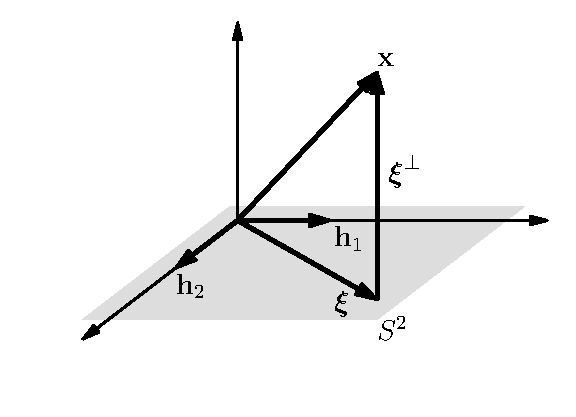
\includegraphics[width=\textwidth]{figuras/problem_8_11.pdf}
  \end{minipage}\hfill
  \begin{minipage}[c]{0.47\textwidth}
    \caption{
       Descomposición del vector \(\x\) para el caso en que \(\x\in R^3\) y la matriz de proyección \(\mathbf{P}\) conduce al subespacio \(S^2\).
    } \label{fig:problem_8_11}
  \end{minipage}
\end{figure}
Considerando esta descomposición, se observa que se cumple que 
\begin{align*}
 \x_1^T\Pbf\x_2-\x_2^T\Pbf\x_1&=(\bm{\xi}_1+\bm{\xi}_1^\perp)^T\Pbf(\bm{\xi}_2+\bm{\xi}_2^\perp)-(\bm{\xi}_2+\bm{\xi}_2^\perp)^T\Pbf(\bm{\xi}_1+\bm{\xi}_1^\perp)\\
  &=(\bm{\xi}_1+\bm{\xi}_1^\perp)^T\Pbf\bm{\xi}_2+(\bm{\xi}_1+\bm{\xi}_1^\perp)^T\Pbf\bm{\xi}_2^\perp-(\bm{\xi}_2+\bm{\xi}_2^\perp)^T\Pbf\bm{\xi}_1-(\bm{\xi}_2+\bm{\xi}_2^\perp)^T\Pbf\bm{\xi}_1^\perp\\
  &\overset{(a)}{=}(\bm{\xi}_1+\bm{\xi}_1^\perp)^T\bm{\xi}_2-(\bm{\xi}_2+\bm{\xi}_2^\perp)^T\bm{\xi}_1\\
  &=\bm{\xi}_1^T\bm{\xi}_2+{\bm{\xi}_1^\perp}^T\bm{\xi}_2-\bm{\xi}_2^T\bm{\xi}_1-{\bm{\xi}_2^\perp}^T\bm{\xi}_1\\
  &\overset{(b)}{=}\bm{\xi}_1^T\bm{\xi}_2-\bm{\xi}_2^T\bm{\xi}_1\\
  &\overset{(c)}{=}0,
\end{align*}
donde en \((a)\) se consideró que como \(\bm{\xi}_i\in S^p\), se cumple que \(\mathbf{P}\bm{\xi}_i=\bm{\xi}_i\), y como \(\bm{\xi}_i^\perp\) es ortogonal a \(S^p\), se cumple que \(\mathbf{P}\bm{\xi}_i^\perp=\mathbf{0}\), en \((b)\) se tuvo en cuenta que \(\bm{\xi}_i\) y \(\bm{\xi}_j^\perp\) son ortogonales y por lo tanto \({\bm{\xi}_i^\perp}^T\bm{\xi}_j\) y en \((c)\) que los sumandos son escalares y por lo tanto, invariantes a la transposición. Para ver que \(\mathbf{P}\) es simétrica se considera la identidad que se acaba de deducir,
\[
 \x_1^T\Pbf\x_2=\x_2^T\Pbf\x_1.
\]
El lado izquierdo de la igualdad se puede escribir como
\[
 \x_1^T\Pbf\x_2=(\x_1^T\Pbf\x_2)^T=\x_2^T\Pbf^T\x_1,
\]
donde nuevamente se tuvo en cuenta que se trata de magnitudes escalares. Finalmente, como
\[
 \x_2^T\Pbf^T\x_1=\x_2^T\Pbf\x_1,
\]
se concluye que \(\Pbf^T=\Pbf\) y por lo tanto, \(\Pbf\) es una matriz simétrica.

\subsection{Problema 12}\label{sec:problem_8_12}

Probar las siguientes propiedades de la matriz de proyección
\[
 \Pbf=\Hbf(\Hbf^T\Hbf)^{-1}\Hbf^T.
\]
\begin{enumerate}[a.]
 \item \(\Pbf\) es idempotente.
 \item \(\Pbf\) es semidefinida positiva.
 \item Los valores propios de \(\Pbf\) son 0 o 1.
 \item El rango de \(\Pbf\) es \(p\). Emplear el hecho de que la traza de una matriz es igual a la suma de sus valores propios.
\end{enumerate}

\paragraph{Solución} Hay que tener en cuenta que si la matriz \(\Hbf\) tiene dimensiones \(N\times p\), la matriz \(\Pbf\) tiene dimensiones \(N\times N\).
\begin{enumerate}[a.]
 \item Efectivamente \(\Pbf\) es idempotente, ya que
 \[
  \Pbf^2=\Hbf(\Hbf^T\Hbf)^{-1}\Hbf^T\Hbf(\Hbf^T\Hbf)^{-1}\Hbf^T=\Hbf(\Hbf^T\Hbf)^{-1}\Hbf^T=\Pbf.
 \]
 \item Para ver que \(\Pbf\) es semidefinida positiva, hay que demostrar que \(\x^T\Pbf\x\geq0\) para todo \(\x\). Se observa que
 \[
  \x^T\Pbf\x\overset{(a)}{=}\x^T\Pbf\Pbf\x\overset{(b)}{=}\x^T\Pbf^T\Pbf\x=(\Pbf\x)^T(\Pbf\x)=\lVert\Pbf\x\rVert^2\geq0,
 \]
 donde en \((a)\) se empleó que \(\Pbf\) es idempotente, como se mostró en a., y en \((b)\) que \(\Pbf\) es simétrica, como se demostró en el problema \ref{sec:problem_8_11}.
 \item Los valores propios de una matriz cumplen que \(\Pbf\x=\lambda\x\), con \(\x\neq\mathbf{0}\). Sea \(\x\) un valor propio de \(\Pbf\) con valor propio \(\lambda\) asociado. De esta forma, se cumple que
 \[
  \Pbf\x\overset{(a)}{=}\Pbf\Pbf\x=\Pbf\lambda\x=\lambda\Pbf\x=\lambda^2\x,
 \]
 donde en \((a)\) se consideró que \(\Pbf\) es idempotente, como se demostro en el primer punto.
 Por lo tanto, si \(\lambda\) es el valor propio asociado al vector propio \(\x\), \(\lambda^2\) también es valor propio asociado a \(\x\). Como un vector propio no puede tener mas de un valor propio distinto asociado, se concluye que \(\lambda=0\) o \(\lambda=1\).
 \item Para ver que \(\operatorname{rank}(\Pbf)=p\), se parte considerando que la traza de una matriz es invariable a permutaciones cíclicas, como se muestra en el apéndice \ref{ap:lineal_algebra_basics}. Por lo tanto,
 \[
  \tr(\Pbf)=\tr[\Hbf(\Hbf^T\Hbf)^{-1}\Hbf^T]=\tr[(\Hbf^T\Hbf)^{-1}\Hbf^T\Hbf]\overset{(a)}{=}\tr(\I_{p\times p})=p,
 \]
 donde en \((a)\), \(\I_{p\times p}\) es la matriz identidad de tamaño \(p\times p\), cuya traza es \(p\). Además, como la suma de los valores propios de una matriz coincide con su traza (ver el apéndice \ref{ap:lineal_algebra_basics}), se cumple que
 \[
  \sum_{i=1}^N\lambda_i(\Pbf)=p,
 \]
 y teniendo en cuenta que los valores propios de \(\Pbf\) son 0 o 1, como se demostró en el punto anterior, se deduce que \(\Pbf\) tiene \(p\) valores propios de valor 1 y \(N-p\) valores propios de valor 0. Además, como una matriz real y simétrica tiene rango igual a la cantidad de valores propios distintos de cero por ser diagonalizable (ver el apéndice \ref{ap:lineal_algebra_basics}), se concluye que \(\operatorname{rank}(\Pbf)=p\).
\end{enumerate}

\subsection{Problema 13}\label{sec:problem_8_13}

Comprobar el resultado de la ecuación \ref{eq:ls_lls_line_fitting_estimator} del estimador para el problema del ajuste de una recta.

\paragraph{Solución} El modelo de los datos es
\[
 s[n]=A+Bn,\qquad n=0,\,\dots,\,N-1,
\]
y en forma matricial, se expresa como
\[
 \s=\Hbf\thetabf,\qquad\qquad\textrm{con}\qquad\qquad
 \Hbf=
 \begin{bmatrix}
  1 & 0\\
  1 & 1\\
  \vdots & \vdots\\
  1 & N-1
 \end{bmatrix}\qquad\qquad\textrm{y}\qquad\qquad
 \thetabf=
 \begin{bmatrix}
  A \\ B
 \end{bmatrix}.
\]
Como indica la ecuación \ref{eq:ls_lls_estimator_vector}, el LSE es
\[
 \hat{\thetabf}=(\Hbf^T\Hbf)^{-1}\Hbf^T\x.
\]
En este caso,
\[
 \Hbf^T\Hbf=
 \begin{bmatrix}
  1 & 1 & \dots & 1\\
  0 & 1 & \dots & N-1
 \end{bmatrix}
 \begin{bmatrix}
  1 & 0\\
  1 & 1\\
  \vdots & \vdots\\
  1 & N-1
 \end{bmatrix}=
 \begingroup
 \renewcommand*{\arraystretch}{2.6}
 \begin{bmatrix}
  \displaystyle\sum_{n=0}^{N-1}1 & \displaystyle\sum_{n=0}^{N-1}n\\
  \displaystyle\sum_{n=0}^{N-1}n & \displaystyle\sum_{n=0}^{N-1}n^2
 \end{bmatrix}
 \overset{(a)}{=}N
 \begin{bmatrix}
    1 & \dfrac{N-1}{2}\\
    \dfrac{N-1}{2} & \dfrac{(N-1)(2N-1)}{6}
 \end{bmatrix}.
 \endgroup
\]
donde en \((a)\) se emplearon las identidades dadas por las ecuaciones \ref{eq:sums_of_powers}.
La matriz inversa es
\[
\renewcommand*{\arraystretch}{2.5}
 (\Hbf^T\Hbf)^{-1}=\frac{1}{N}
 \begin{bmatrix}
     \dfrac{2(2N-1)}{N+1} & -\dfrac{6}{N+1}\\
     -\dfrac{6}{N+1} & \dfrac{12}{N^2-1}
 \end{bmatrix},
\]
como se calculó en el ejemplo de la sección \ref{sec:line_fitting} (ver la ecuación \ref{eq:line_fitting_covariance}). Además, se tiene que
\[
 \Hbf^T\x=\begin{bmatrix}
  1 & 1 & \dots & 1\\
  0 & 1 & \dots & N-1
 \end{bmatrix}
 \begin{bmatrix}
  x[0] \\ \vdots \\ x[N-1]
 \end{bmatrix}=
 \begingroup
 \renewcommand*{\arraystretch}{2.6}
 \begin{bmatrix}
  \displaystyle\sum_{n=0}^{N-1}x[n]\\
  \displaystyle\sum_{n=0}^{N-1}nx[n]
 \end{bmatrix}.
 \endgroup
\]
Combinando los resultados, se obtiene que
\[
 \begin{bmatrix}
  \hat{A} \\ \hat{B}
 \end{bmatrix}=
 \renewcommand*{\arraystretch}{2.5}
 \frac{1}{N}
 \begin{bmatrix}
     \dfrac{2(2N-1)}{N+1} & -\dfrac{6}{N+1}\\
     -\dfrac{6}{N+1} & \dfrac{12}{N^2-1}
 \end{bmatrix}
 \begin{bmatrix}
  \displaystyle\sum_{n=0}^{N-1}x[n]\\
  \displaystyle\sum_{n=0}^{N-1}nx[n]
 \end{bmatrix},
\]
resultando en
\begin{align*}
  \hat{A}&=\frac{2(2N-1)}{N(N+1)}\sum_{n=0}^{N-1}x[n]-\frac{6}{N(N+1)}\sum_{n=0}^{N-1}nx[n]\\
  \hat{B}&=-\frac{6}{N(N+1)}\sum_{n=0}^{N-1}x[n]+\frac{12}{N(N^2-1)}\sum_{n=0}^{N-1}nx[n],
\end{align*}
que es lo que  se quería mostrar. Notar que el estimador coincide con el estimador eficiente cuando el ruido es WGN del ejemplo de la sección \ref{sec:line_fitting}. Sin embargo, no se puede asegurar que el LSE obtenido sea eficiente debido a que no están especificadas las características estadísticas del ruido.

\subsection{Problema 14}\label{sec:problem_8_14}

En este problema se derivan las ecuaciones de actualización del algortimo LS de orden recursivo emplando un enfoque geométrico. Asúmase que se dispone de \(\hat{\thetabf}_k\) y por lo tanto se conoce
\begin{equation}\label{eq:problem_8_14_hat_s_k}
 \hat{\s}_k=\Hbf_k\hat{\thetabf}_k.
\end{equation}
Si se agrega la columna \(\h_{k+1}\) a la matriz de observación, el la señal LS estimada es
\[
 \hat{\s}_{k+1}=\hat{\s}_k+\alpha\h_{k+1}',
\]
donde \(\h_{k+1}'\) es el componente de \(\h_{k+1}\) ortogonal al subespacio generado por \(\{\h_1,\,\dots,\,\h_k\}\). En primer lugar, encontrar \(\h_{k+1}'\) y luego determinar \(\alpha\) notando que \(\alpha\h_{k+1}'\) es la proyección de \(\x\) en \(\h_{k+1}'\). Finalmente, como
\[
 \hat{\s}_{k+1}=\Hbf_{k+1}\hat{\thetabf}_{k+1}
\]
determinar \(\hat{\thetabf}_{k+1}\).

\paragraph{Solución} Como se discute en la sección \ref{sec:ls_lls_geometric_interpretation}, la matriz de proyección del subespacio generado por las columnas de \(\Hbf_k\) es \(\Pbf_{k}=\Hbf(\Hbf_k^T\Hbf_k)\Hbf_k^T\) y la matriz de proyección del subespacio ortogonal es \(\Pbf_k^\perp=\I-\Pbf_k\). Por lo tanto, la proyección de \(\h_{k+1}\) en el subespacio ortogonal al generado por las columnas de \(\Hbf_k\) es
\begin{equation}\label{eq:problem_8_14_h_k+1_proj}
 \h_{k+1}'=\Pbf_k^\perp\h_{k+1}.
\end{equation}
Para determinar \(\alpha\), se parte notando que dados dos vectores \(\ubf\) y \(\vbf\), el vector proyección \(\operatorname{proj}_\ubf(\vbf)\) de \(\vbf\) sobre \(\ubf\) es\footnote{Ver \href{https://en.wikipedia.org/wiki/Gram\%E2\%80\%93Schmidt_process}{https://en.wikipedia.org/wiki/Gram-Schmidt\_process}}
\[
 \operatorname{proj}_\ubf(\vbf)=\frac{\ubf^T\vbf}{\lVert\ubf\rVert^2}\ubf.
\]
Efectivamente, la matriz de proyección sobre el subespacio generado por \(\ubf\) es 
\[
 \Pbf=\ubf(\ubf^T\ubf)^{-1}\ubf^T=\frac{\ubf\ubf^T}{\ubf^T\ubf}=\frac{\ubf\ubf^T}{\lVert\ubf\rVert^2},
\]
y por lo tanto, la proyección de \(\vbf\) sobre ese subespacio es
\[
 \operatorname{proj}_\ubf(\vbf)=\Pbf\vbf=\frac{\ubf\ubf^T}{\lVert\ubf\rVert^2}\vbf\overset{(a)}{=}\frac{\ubf^T\vbf}{\lVert\ubf\rVert^2}\ubf.
\]
donde en \((a)\) se tuvo en cuenta que \([\ubf^T\ubf]_{ij}=\ubf_i\ubf_j\) y por lo tanto
\[
 [(\ubf^T\ubf)\vbf]_i=\sum_{j}\ubf_i\ubf_j\vbf_j=\ubf_i(\ubf^T\vbf)=[(\ubf^T\vbf)\ubf]_i.
\]
Con estas consideraciones, la proyección de \(\x\) sobre \(\h_{k+1}'\) es
\[
 \alpha\h_{k+1}'=\frac{\h_{k+1}'^T\x}{\lVert\h_{k+1}'\rVert^2}\h_{k+1}',
\]
y por lo tanto
\[
 \alpha=\frac{\h_{k+1}'^T\x}{\lVert\h_{k+1}'\rVert^2}=\frac{\h_{k+1}^T{\Pbf_k^\perp}^T\x}{\lVert\Pbf_k^\perp\h_{k+1}\rVert^2}=\frac{\h_{k+1}^T{\Pbf_k^\perp}^T\x}{\h_{k+1}^T{\Pbf_k^\perp}^T\Pbf_k^\perp\h_{k+1}}.
\]
Además, considerando que \(\Pbf_k^\perp\) es una matriz simétrica e idempotente por ser una matriz de proyección, se obtiene que
\begin{equation}\label{eq:problem_8_14_alpha}
 \alpha=\frac{\h_{k+1}^T\Pbf_k^\perp\x}{\h_{k+1}^T\Pbf_k^\perp\h_{k+1}}.
\end{equation}
La señal LS estimada en el paso \(k+1\) es
\begin{align*}
 \hat{\s}_{k+1}&=\hat{\s}_k+\alpha\h_{k+1}'\\
  &\overset{(a)}{=}\Hbf_k\hat{\thetabf}_k+\frac{\h_{k+1}^T\Pbf_k^\perp\x}{\h_{k+1}^T\Pbf_k^\perp\h_{k+1}}\Pbf_k^\perp\h_{k+1}\\
  &\overset{(b)}{=}\Hbf_k\hat{\thetabf}_k+(\I-\Pbf_k)\h_{k+1}\frac{\h_{k+1}^T\Pbf_k^\perp\x}{\h_{k+1}^T\Pbf_k^\perp\h_{k+1}}\\
  &=\Hbf_k\hat{\thetabf}_k+\frac{\h_{k+1}\h_{k+1}^T\Pbf_k^\perp\x}{\h_{k+1}^T\Pbf_k^\perp\h_{k+1}}-\frac{\Pbf_k\h_{k+1}\h_{k+1}^T\Pbf_k^\perp\x}{\h_{k+1}^T\Pbf_k^\perp\h_{k+1}}\\
  &\overset{(c)}{=}\Hbf_k\hat{\thetabf}_k+\frac{\h_{k+1}\h_{k+1}^T\Pbf_k^\perp\x}{\h_{k+1}^T\Pbf_k^\perp\h_{k+1}}-\frac{\Hbf_k(\Hbf_k^T\Hbf_k)^{-1}\Hbf_k^T\h_{k+1}\h_{k+1}^T\Pbf_k^\perp\x}{\h_{k+1}^T\Pbf_k^\perp\h_{k+1}}\\
  &=
  \begin{bmatrix}
   \Hbf_k & \h_{k}
  \end{bmatrix}
  \renewcommand*{\arraystretch}{2.6}
  \begin{bmatrix}
   \hat{\thetabf}_k-\dfrac{(\Hbf_k^T\Hbf_k)^{-1}\Hbf_k^T\h_{k+1}\h_{k+1}^T\Pbf_k^\perp\x}{\h_{k+1}^T\Pbf_k^\perp\h_{k+1}}\\
   \dfrac{\h_{k+1}^T\Pbf_k^\perp\x}{\h_{k+1}^T\Pbf_k^\perp\h_{k+1}}
  \end{bmatrix}\\
  &=\Hbf_{k+1}\hat{\thetabf}_{k+1}
\end{align*}
donde en \((a)\) se sustituyeron las ecuaciones \ref{eq:problem_8_14_hat_s_k}, \ref{eq:problem_8_14_h_k+1_proj} y \ref{eq:problem_8_14_alpha}, en \((b)\) se consideró que \(\Pbf_k^\perp=\I-\Pbf_k\) y en \((c)\) que \(\Pbf_k=\Hbf_k(\Hbf_k^T\Hbf_k)^{-1}\Hbf_k^T\). Se concluye que \(\hat{\thetabf}_{k+1}\) está dado por la ecuación \ref{eq:ls_order_recursive_theta_update}.

\subsection{Problema 15}

Emplear el algoritmo LS de orden recursivo para encontrar los valores de \(A\) y \(B\) que minimizan 
\[
 J=\sum_{n=0}^{N-1}(x[n]-A-Br^n)^2.
\]
Se asume que el parámetro \(r\) es conocido.

\paragraph{Solución} El modelo de señal de orden 1 es
\[
 s_1[n]=A_1,
\]
que en forma matricial se expresa como
\[
 \s_1=\Hbf_1A_1,\qquad\qquad\textrm{con}\qquad\qquad\Hbf_1=\mathbf{1},
\]
por lo que el estimador de orden 1 es
\[
 \hat{A}_1=(\Hbf_1^T\Hbf_1)^T\Hbf_1^T\x=(\mathbf{1}^T\mathbf{1})^T\mathbf{1}^T\x=\frac{1}{N}\sum_{n=0}^{N-1}x[n],
\]
es decir,
\[
 \hat{\thetabf}_1=\hat{A}_1=\bar{x}.
\]
El modelo de señal de orden 2 es
\[
 s_2[n]=A_2+B_2r^n
\]
y en forma matricial se expresa como
\[
 \s_2=\Hbf_2\thetabf_2,\qquad\textrm{con}\qquad
 \Hbf_2=
 \begin{bmatrix}
  1 & 1\\
  1 & r\\
  1 & r^2\\
  \vdots & \vdots\\
  1 & r^{N-1}
 \end{bmatrix}
 =\begin{bmatrix}
   \Hbf_1 & \h_2
  \end{bmatrix}
  \qquad\textrm{y}\qquad
  \thetabf_2=
  \begin{bmatrix}
   A\\B
  \end{bmatrix}.
\]
La actualización al estimador de orden 2 en el LS recursivo está dado por la ecuación \ref{eq:ls_order_recursive_theta_update} y es
\[
\begingroup
\renewcommand*{\arraystretch}{2.6}
 \hat{\thetabf}_2=
 \begin{bmatrix}
  \hat{\thetabf}_1-\dfrac{(\Hbf^T_1\Hbf_1)^{-1}\Hbf^T_1\h_2\h_2^T\Pbf_1^\perp\x}{\h_2^T\Pbf_1^\perp\h_2}\\
  \dfrac{\h_2^T\Pbf_1^\perp\x}{\h_2^T\Pbf_1^\perp\h_2}
 \end{bmatrix}
\endgroup
\]
donde
\[
 \Pbf_1^\perp=\I-\Hbf_1(\Hbf^T_1\Hbf_1)^{-1}\Hbf^T_1.
\]
Empleando las definiciones, se tiene que
\[
 (\Hbf_1^T\Hbf_1)^{-1}=\frac{1}{N},\qquad\Pbf_1^\perp=\I-\frac{1}{N}\mathbf{1}\mathbf{1}^T,
 \qquad
 \Pbf_1^\perp\x=\x-\frac{1}{N}\mathbf{1}\mathbf{1}^T\x=\x-\frac{1}{N}\mathbf{1}\sum_{n=0}^{N-1}x[n]=\x-\mathbf{1}\bar{x}
\]
\[
 \h_2^T\Pbf_1^\perp\x=\h_2^T\x-\h_2^T\mathbf{1}\bar{x}=\sum_{n=0}^{N-1}x[n]r^n-\bar{x}\sum_{n=0}^{N-1}r^n,
 \qquad\qquad
 (\Hbf_1^T\Hbf_1)^{-1}\Hbf_1^T\h_2=\frac{1}{N}\sum_{n=0}^{N-1}r^n
\]
\[
 \h_2^T\Pbf_1^\perp\h_2=\h_2^T\h_2-\frac{1}{N}\h_2^T\mathbf{1}\mathbf{1}^T\h_2=\h_2^T\h_2-\frac{1}{N}(\h_2^T\mathbf{1})^2=\sum_{n=0}^{N-1}r^{2n}-\frac{1}{N}\left(\sum_{n=0}^{N-1}r^n\right)^2,
\]
y sustituyendo en la actualización del estimador, se obtiene que
\[
\begingroup
\renewcommand*{\arraystretch}{5.4}
 \hat{\thetabf}_2=
 \begin{bmatrix}
  \bar{x}-\dfrac{\displaystyle\frac{1}{N}\sum_{n=0}^{N-1}r^n\left(\sum_{n=0}^{N-1}x[n]r^n-\bar{x}\sum_{n=0}^{N-1}r^n\right)}{\displaystyle\sum_{n=0}^{N-1}r^{2n}-\frac{1}{N}\left(\sum_{n=0}^{N-1}r^n\right)^2}\\
  \dfrac{\displaystyle\sum_{n=0}^{N-1}x[n]r^n-\bar{x}\sum_{n=0}^{N-1}r^n}{\displaystyle\sum_{n=0}^{N-1}r^{2n}-\frac{1}{N}\left(\sum_{n=0}^{N-1}r^n\right)^2}
 \end{bmatrix},
\endgroup
\]
es decir,
\[
 \hat{A}_2=\bar{x}-\frac{1}{N}\sum_{n=0}^{N-1}r^n\hat{B}_2,\qquad\qquad\hat{B}_2=\dfrac{\displaystyle\sum_{n=0}^{N-1}x[n]r^n-\bar{x}\sum_{n=0}^{N-1}r^n}{\displaystyle\sum_{n=0}^{N-1}r^{2n}-\frac{1}{N}\left(\sum_{n=0}^{N-1}r^n\right)^2}.
\]

\subsection{Problema 16}

Se consideran los modelos
\[
\begingroup
\renewcommand*{\arraystretch}{2}
 \begin{array}{cclcc}
  s_1[n]&=&A\quad0\leq n\leq N-1\\
  s_2[n]&=&\left\{
  \begingroup
  \renewcommand*{\arraystretch}{1}
   \begin{array}{ll}
    A & 0\leq n \leq M-1\\
    B & M\leq n \leq N-1.
   \end{array}\endgroup\right.
 \end{array}
\endgroup
\]
La segunda señal es útil para modelar un salto del nivel en \(n=M\). Alternativamente, el segundo modelo se puede expresar como
\[
 s_2[n]=Au_1[n]+(B-A)u_2[n]
\]
donde
\[
\begingroup
\renewcommand*{\arraystretch}{2}
 \begin{array}{cclcc}
  u_1[n]&=&1\quad0\leq n\leq N-1\\
  u_2[n]&=&\left\{
  \begingroup
  \renewcommand*{\arraystretch}{1}
   \begin{array}{ll}
    0 & 0\leq n \leq M-1\\
    1 & M\leq n \leq N-1.
   \end{array}\endgroup\right.
 \end{array}
\endgroup
\]
Sea \(\thetabf_1=A\) y \(\thetabf_2=[A\;(B-A)]^T\). Encontrar el LSE y el error LS mínimo para cada modelo empleando el LS de orden recursivo. Discutir como podría emplear los resultados para detectar un salto en el nivel. 

\paragraph{Solución} El modelo la primer señal es
\[
 \s_1=\Hbf_1A_1,\qquad\qquad\textrm{con}\qquad\qquad\Hbf_1=\mathbf{1},
\]
por lo que, al igual que el problema anterior, el estimador 
\[
 \hat{\thetabf}_1=\hat{A}_1=\bar{x}.
\]
El modelo de señal de orden 2 es
\[
 \s_2=\begin{bmatrix}
   \Hbf_1 & \h_2
  \end{bmatrix}
 \thetabf_2,\qquad\textrm{con}\qquad
 \begin{array}{ccrccccccl}
 \h_2 & = & [ & 0                  & \dots & 0 & 1                  & \dots & 1 & ]^T\\
      &   &   & {\scriptstyle n=0} &       &   & {\scriptstyle n=M} &       &   &
\end{array}
  \qquad\textrm{y}\qquad
  \thetabf_2=
  \begin{bmatrix}
   A\\B-A
  \end{bmatrix}.
\]
La actualización al estimador de orden 2 en el LS recursivo está dado por la ecuación \ref{eq:ls_order_recursive_theta_update} con 
\[
 (\Hbf_1^T\Hbf_1)^{-1}=\frac{1}{N},\qquad\Pbf_1^\perp=\I-\frac{1}{N}\mathbf{1}\mathbf{1}^T,
 \qquad
 \Pbf_1^\perp\x=\x-\frac{1}{N}\mathbf{1}\mathbf{1}^T\x=\x-\frac{1}{N}\mathbf{1}\sum_{n=0}^{N-1}x[n]=\x-\mathbf{1}\bar{x}
\]
ya que \(\Hbf_1=\mathbf{1}\) al igual que el problema anterior. Además, considerando la definición de \(\h_2\), 
\[
 \h_2^T\Pbf_1^\perp\x=\h_2^T\x-\h_2^T\mathbf{1}\bar{x}=\sum_{n=M}^{N-1}x[n]-(N-M)\bar{x},
 \qquad\qquad
 (\Hbf_1^T\Hbf_1)^{-1}\Hbf_1^T\h_2=\frac{N-M}{N},
\]
\[
 \h_2^T\Pbf_1^\perp\h_2=\h_2^T\h_2-\frac{1}{N}\h_2^T\mathbf{1}\mathbf{1}^T\h_2=\h_2^T\h_2-\frac{1}{N}(\h_2^T\mathbf{1})^2=(N-M)-\frac{1}{N}(N-M)^2=\frac{M}{N}(N-M).
\]
Por lo tanto, el estimador es
\begin{align*}
 \hat{A}_2&=\hat{\thetabf}_1-\dfrac{(\Hbf^T_1\Hbf_1)^{-1}\Hbf^T_1\h_2\h_2^T\Pbf_1^\perp\x}{\h_2^T\Pbf_1^\perp\h_2}\\
  &=\bar{x}-\dfrac{\displaystyle\frac{N-M}{N}\left[\sum_{n=M}^{N-1}x[n]-(N-M)\bar{x}\right]}{\dfrac{M}{N}(N-M)}\\
  &=\bar{x}-\frac{1}{M}\sum_{n=M}^{N-1}x[n]+\frac{N-M}{M}\bar{x}\\
  &=-\frac{1}{M}\sum_{n=M}^{N-1}x[n]+\frac{N}{M}\bar{x}\\
  &=-\frac{1}{M}\sum_{n=M}^{N-1}x[n]+\frac{1}{M}\left(\sum_{n=0}^{M-1}x[n]+\sum_{n=M}^{N-1}x[n]\right)\\
  &=\frac{1}{M}\sum_{n=0}^{M-1}x[n]
\end{align*}
resultando en
\[
 \hat{A}_2=\frac{1}{M}\sum_{n=0}^{M-1}x[n],
\]
y
\begin{align*}
 \widehat{B-A}&=\dfrac{\h_2^T\Pbf_1^\perp\x}{\h_2^T\Pbf_1^\perp\h_2}\\
  &=\dfrac{\displaystyle\sum_{n=M}^{N-1}x[n]-(N-M)\bar{x}}{\dfrac{M}{N}(N-M)}\\
  &=\frac{M}{N}\left(\frac{1}{N-M}\sum_{n=M}^{N-1}x[n]-\bar{x}\right),
\end{align*}
resultando en
\[
 \widehat{B-A}=\frac{M}{N}(\bar{x}_1-\bar{x}),\qquad\qquad\textrm{con}\qquad\qquad\bar{x}_1=\frac{1}{N-M}\sum_{n=M}^{N-1}x[n].
\]
De la ecuación \ref{eq:ls_lls_min_error_vector}, el error mínimo en el estimador de primer orden es
\begin{align*}
 J_{\min_1}&=\x^T\Pbf_1^\perp\x\\
  &=\x^T(\x-\mathbf{1}\bar{x})\\
  &=\sum_{n=0}^{N-1}x^2[n]-\bar{x}\sum_{n=0}^{N-1}x[n],
\end{align*}
resultando en
\[
 J_{\min_1}=\sum_{n=0}^{N-1}x^2[n]-N\bar{x}^2.
\]
La actualización del error LS para el modelo de segundo orden está dado por la ecuación \ref{eq:ls_order_recursive_Jmin_update},
\[
 J_{\min_2}=J_{\min_1}-\frac{(\h_2^T\Pbf_1^\perp\x)^2}{\h_2^T\Pbf_1^\perp\h_2}.
\]
El decremento del error es
\begin{align*}
 \frac{(\h_2^T\Pbf_1^\perp\x)^2}{\h_2^T\Pbf_1^\perp\h_2}&=(\h_2^T\Pbf_1^\perp\x)\frac{(\h_2^T\Pbf_1^\perp\x)}{\h_2^T\Pbf_1^\perp\h_2}\\
 &\overset{(a)}{=}(N-M)(\bar{x}_1-\bar{x})\widehat{B-A}\\
 &=(N-M)(\bar{x}_1-\bar{x})\frac{M}{N}(\bar{x}_1-\bar{x})
\end{align*}
\begin{align*}
 \frac{(\h_2^T\Pbf_1^\perp\x)^2}{\h_2^T\Pbf_1^\perp\h_2}&=(\h_2^T\Pbf_1^\perp\x)\frac{(\h_2^T\Pbf_1^\perp\x)}{\h_2^T\Pbf_1^\perp\h_2}\\
 &=\left(\sum_{n=M}^{N-1}x[n]-(N-M)\bar{x}\right)\widehat{B-A}\\
 &=(N-M)(\bar{x}_1-\bar{x})\frac{M}{N}(\bar{x}_1-\bar{x})
\end{align*}
resultando en
\[
 J_{\min_2}=J_{\min_1}-\frac{M}{N}(N-M)(\bar{x}_1-\bar{x})^2.
\]
Un salto en el nivel en \(n=M\) se manifiesta en un decrecimiento grande del error \(J_{\min_2}\) del modelo de segundo orden. Efectivamente, si no hay un cambio de nivel \(\bar{x}_1\approx\bar{x}\) y por lo tanto \(J_{\min_2}\approx J_{\min_1}\), mientras si hay un cambio de nivel, \((\bar{x}_1-\bar{x})^2\) tendrá un valor significativo.

\subsection{Problema 17}

Probar que \(\Pbf^\perp_k\x\) es ortogonal al subespacio generado por las columnas de \(\Hbf_k\).

\paragraph{Solución} Hay que probar que
\[
 \Hbf_k^T\Pbf^\perp_k\x=\mathbf{0}.
\]
Considerando la definición de la matriz de proyección \(\Pbf^\perp_k\), dada por la ecuación \ref{eq:ls_order_recursive_p_k_definition}, se tiene que
\begin{align*}
 \Hbf_k^T\Pbf^\perp_k\x&=\Hbf_k(\I-\Hbf_k(\Hbf^T_k\Hbf_k)^{-1}\Hbf^T_k)\x\\
   &=\Hbf_k^T\x-\Hbf_k^T\Hbf_k(\Hbf^T_k\Hbf_k)^{-1}\Hbf^T_k\x\\
   &=\Hbf_k^T\x-\Hbf^T_k\x\\
   &=\mathbf{0}.
\end{align*}

\subsection{Problema 18}\label{sec:problem_8_18}

Empleando la matriz de proyección ortogonal recursiva (ecuación \ref{eq:ls_order_recursive_P_update}) derivar la actualización del error LS mínimo (ecuación \ref{eq:ls_order_recursive_Jmin_update}).

\paragraph{Solución} Partiendo de la ecuación \ref{eq:ls_lls_min_error_vector} del error LS mínimo, se tiene que 
\begin{align*}
 J_{\textrm{min}_{k+1}}&=\x^T(\I-\Pbf_{k+1})\x\\
  &=\x^T\x-\x^T\Pbf_{k+1}\x\\
  &=\x^T\x-\x^T\left[\Pbf_k+\frac{(\I-\Pbf_k)\h_{k+1}\h_{k+1}^T(\I-\Pbf_k)}{\h_{k+1}^T(\I-\Pbf_k)\h_{k+1}}\right]\x\\
  &=\x^T\x-\x^T\Pbf_k\x-\frac{\x^T\Pbf_k^\perp\h_{k+1}\h_{k+1}^T\Pbf_k^\perp\x}{\h_{k+1}^T\Pbf_k^\perp\h_{k+1}}\\
  &=J_{\textrm{min}_k}-\frac{(\h_{k+1}^T\Pbf_k^\perp\x)^2}{\h_{k+1}^T\Pbf_k^\perp\h_{k+1}}.
\end{align*}

\subsection{Problema 19}\label{sec:problem_8_19}

Verificar la ecuación \ref{eq:ls_sls_no_corraleted_noise_jmin} del cálculo secuencial del error LS mínimo empleando la ecuación \ref{eq:ls_sls_no_corraleted_noise_estimator} de la actualización del LSE. 

\paragraph{Solución} En el problema de la estimación del nivel de DC en ruido no correlacionado el LSE se obtiene minimizando el error LS ponderado (ver el problema \ref{sec:problem_8_8})
\[
 J(A)=\sum_{n=0}^{N-1}\frac{1}{\sigma_n^2}(x[n]-A)^2.
\]
Para obtener la expresión recursiva del error LS mínimo se observa que
\begin{align*}
 J_\textrm{min}[N]&=\sum_{n=0}^{N}\frac{1}{\sigma_n^2}(x[n]-\hat{A}[N])^2\\
  &=\sum_{n=0}^{N-1}\frac{1}{\sigma_n^2}(x[n]-\hat{A}[N])^2+\frac{1}{\sigma_N^2}(x[N]-\hat{A}[N])^2\\
  &\overset{(a)}{=}\sum_{n=0}^{N-1}\frac{1}{\sigma_n^2}\left[x[n]-\hat{A}[N-1]-K[N](x[N]-\hat{A}[N-1])\right]^2\\
  &\quad+\frac{1}{\sigma_N^2}\left[x[N]-\hat{A}[N-1]-K[N](x[N]-\hat{A}[N-1])\right]^2\\
  &=\sum_{n=0}^{N-1}\frac{1}{\sigma_n^2}(x[n]-\hat{A}[N-1])^2+
  2K[N](x[N]-\hat{A}[N-1])\sum_{n=0}^{N-1}\frac{1}{\sigma_n^2}(x[n]-\hat{A}[N-1])\\
  &\quad+K^2[N](x[N]-\hat{A}[N-1])^2\sum_{n=0}^{N-1}\frac{1}{\sigma_n^2}+\frac{1}{\sigma_N^2}\left[x[N]-\hat{A}[N-1]-K[N](x[N]-\hat{A}[N-1])\right]^2,
\end{align*}
donde en \((a)\) se sustituyó \(\hat{A}[N]\) empleando la ecuación \ref{eq:ls_sls_no_corraleted_noise_estimator}. El primer sumando es \(J_\textrm{min}[N-1]\) y la sumatoria del segundo sumando es nula (ver el problema \ref{sec:problem_8_8}). Operando con los dos últimos sumandos se tiene que
\begin{align*}
 &K^2[N](x[N]-\hat{A}[N-1])^2\sum_{n=0}^{N-1}\frac{1}{\sigma_n^2}+\frac{1}{\sigma_N^2}\left[x[N]-\hat{A}[N-1]-K[N](x[N]-\hat{A}[N-1])\right]^2\\
 &\overset{(a)}{=}\frac{K^2[N]}{\var(\hat{A}[N-1])}(x[N]-\hat{A}[N-1])^2+\frac{1}{\sigma_N^2}(x[N]-\hat{A}[N-1])^2(1-K[N])^2\\
 &=(x[N]-\hat{A}[N-1])^2\left[\frac{K^2[N]}{\var(\hat{A}[N-1])}+\frac{1}{\sigma_N^2}(1-K[N])^2\right]\\
 &\overset{(b)}{=}(x[N]-\hat{A}[N-1])^2\left[\frac{\var(\hat{A}[N-1])}{(\var(\hat{A}[N-1])+\sigma^2_N)^2}+\frac{\sigma_N^2}{(\var(\hat{A}[N-1])+\sigma^2_N)^2}\right]\\
 &=\frac{(x[N]-\hat{A}[N-1])^2}{\var(\hat{A}[N-1])+\sigma^2_N},
\end{align*}
donde en \((a)\) se empleó que                                                                                                                                                                                                                                                                                                                                                                                                                                                                                                                                                                                                                                                                                                                                                                                                                                                                                                                                                                                                                                                                                                                                                                       
\[
 \var(\hat{A}[N-1])=\frac{1}{\displaystyle\sum_{n=0}^{N-1}\frac{1}{\sigma_n^2}},
\]                                               
como se encontró en el problema de la sección \ref{sec:problem_8_8} y en \((b)\) se empleó la ecuación \ref{eq:ls_sls_no_corraleted_noise_gain}, que indica que
\[
 K[N]=\frac{\var(\hat{A}[N-1])}{\var(\hat{A}[N-1])+\sigma_N^2}
 \qquad\Rightarrow\qquad
 K[N]-1=\frac{\sigma_N^2}{\var(\hat{A}[N-1])+\sigma_N^2}.
\]
Se concluye que
\[
 J_\textrm{min}[N]=J_\textrm{min}[N-1]+\frac{(x[N]-\hat{A}[N-1])^2}{\var(\hat{A}[N-1])+\sigma^2_N},
\]
que es lo que se quería probar.

\subsection{Problema 20}

Sea \(x[n]=Ar^n+w[n]\), donde \(w[n]\) es WGN de varianza \(\sigma^=1\). Encontrar el LSE secuencial de \(A\) asumiendo que \(r\) es conocido. Además, determinar la varianza del LSE de forma secuencial y luego resolver para obtener una función explícita de \(n\) para la varianza. Tómese \(\hat{A}[0]=x[0]\) y \(\var(\hat{A}[0])=\sigma^2=1\).

\paragraph{Solución} El LSE secuencial está dado por las ecuaciones \ref{eq:ls_sequential_estimator_update}-\ref{eq:ls_sequential_covariance_update}. En este caso, el modelos de la señal es
\[
 \s[n]=\Hbf[n]A,\qquad\qquad\textrm{con}\qquad\qquad 
 \Hbf[n]=
 \begin{bmatrix}
  1&r&r^2&\dots&r^n
 \end{bmatrix}^T,
\]
y por lo tanto, 
\[
 \h[n]=r^n
\]
escalar. Además, como el estimador es escalar, la matriz de covarianza es la varianza del estimador,
\[
 \bm{\Sigma}[n]=\var(\hat{A}[n]).
\]
Por lo tanto, el LSE secuencial es
\[
 \hat{A}[n]=\hat{A}[n-1]+K[n]\left(x[n]-\hat{A}[n-1]r^n\right)
\]
donde
\[
 K[n]=\frac{\var(\hat{A}[n-1])r^n}{1+\var(\hat{A}[n-1])r^{2n}}
\]
y
\[
 \var(\hat{A}[n])=(1-K[n]r^n)\var(\hat{A}[n-1]).
\]
Para resolver la recursión de la varianza, defínase \(v_n=\var(\hat{A}[n])\). De esta forma, sustituyendo la ganancia en la ecuación de la recursión de la varianza, se tiene que
\begin{align*}
 v_n&=\left(1-\frac{v_{n-1}r^{2n}}{1+v_{n-1}r^{2n}}\right)v_{n-1}\\
  &=\frac{v_{n-1}}{1+v_{n-1}r^{2n}}.
\end{align*}
Para simplificar las cuentas, considérese
\[
 \frac{1}{v_n}=\frac{1+v_{n-1}r^{2n}}{v_{n-1}}=\frac{1}{v_{n-1}}+r^{2n}.
\]
Los primeros términos de la recursión son
\[
 \frac{1}{v_0}=1,\qquad \frac{1}{v_1}=\frac{1}{v_0}+r^{2}=1+r^2,\qquad\frac{1}{v_2}=\frac{1}{v_1}+r^4=1+r^2+r^{4},
 \qquad\frac{1}{v_3}=\frac{1}{v_2}+r^6=1+r^2+r^{4}+r^{6}
\]
y en general se cumple que
\[
 \frac{1}{v_n}=\sum_{k=0}^nr^{2k},
\]
concluyendo que
\[
 v_n=\var(\hat{A}[n])=\frac{1}{\displaystyle\sum_{k=0}^nr^{2k}}.
\]

\subsection{Problema 21}

Empleando las ecuaciones \ref{eq:ls_sls_no_corraleted_noise_gain} y \ref{eq:ls_sls_no_corraleted_noise_variance} de la actualización de la ganancia y la varianza respectivamente del LSE secuencial, resolver para las secuencias ganancia y  varianza si \(\sigma_n^2=r^n\). Emplear \(\var(\hat{A}[0])=\var(x[0])=\sigma_0^2=1\) para la inicialización. Luego, examinar que ocurre con la ganancia y la varianza cuando \(N\to\infty\) si \(r=1\), \(0<r<1\) y \(r>1\). Sugerencia: resolver para \(1/\var(\hat{A}[N])\).

\paragraph{Solución} Las ecuaciones de la ganacia y la varianza son respectivamente
\[
 K[N]=\frac{\var(\hat{A}[N-1])}{\var(\hat{A}[N-1])+\sigma_N^2}\qquad\qquad\textrm{y}\qquad\qquad\var(\hat{A}[N])=\left(1-K[N]\right)\var(\hat{A}[N-1]).
\]
Sea \(v_N=\var(\hat{A}[N])\). Sustituyendo la ecuación de la ganancia en la ecuación de la varianza y considerando que \(\sigma_N^2=r^N\) se tiene que
\[
 v_N=\left(1-\frac{v_{N-1}}{v_{N-1}+r^N}\right)v_{N-1}=\frac{v_{N-1}r^N}{v_{N-1}+r^N},
\]
y por lo tanto,
\[
 \frac{1}{v_N}=\frac{v_{N-1}+r^N}{v_{N-1}r^N}=\frac{1}{r^N}+\frac{1}{v_{N-1}}.
\]
Los primeros términos de la recursión son
\[
 \frac{1}{v_0}=1,\qquad\frac{1}{v_1}=\frac{1}{r}+\frac{1}{v_0}=\frac{1}{r}+1,\qquad
  \frac{1}{v_2}=\frac{1}{r^2}+\frac{1}{v_1}=\frac{1}{r^2}+\frac{1}{r}+1,\qquad
  \frac{1}{v_3}=\frac{1}{r^3}+\frac{1}{v_2}=\frac{1}{r^3}+\frac{1}{r^2}+\frac{1}{r}+1,
\]
y generalizando, se obtiene que
\[
 \frac{1}{v_N}=\sum_{n=0}^Nr^{-n}.
\]
Multiplicando y dividiendo el lado derecho de la igualdad entre \(r^N\), el inverso de la varianza se puede expresar como
\[
 \frac{1}{v_N}=\frac{\displaystyle\sum_{n=0}^Nr^{N-n}}{r^N}=\frac{\displaystyle\sum_{k=0}^Nr^k}{r^N},
\]
donde en la segunda igualdad se realizó el cambio de variable \(k=N-n\). Se concluye que la secuencia de la varianza es
\[
 v_N=\var(\hat{A}[N])=\frac{r^N}{\displaystyle\sum_{n=0}^Nr^n}.
\]
Sustituyendo este resultado en la ecuación de la ganancia, se tiene que
\[
 K[N]=\frac{\frac{\displaystyle r^{N-1}}{\displaystyle\sum_{n=0}^{N-1}r^n}}{\frac{\displaystyle r^{N-1}}{\displaystyle\sum_{n=0}^{N-1}r^n}+r^N}
 =\frac{r^{N-1}}{r^{N-1}+r^N\displaystyle\sum_{n=0}^{N-1}r^n}
 =\frac{1}{1+r\displaystyle\sum_{n=0}^{N-1}r^n}
 =\frac{1}{1+\displaystyle\sum_{n=0}^{N-1}r^{n+1}}
 =\frac{1}{1+\displaystyle\sum_{k=1}^{N}r^{k}},
\]
donde en la última igualdad se realizó el cambio de variable \(k=n+1\). Se concluye que
\[
 K[N]=\frac{1}{\displaystyle\sum_{n=0}^{N}r^{n}}.
\]
A continuación se realiza el estudio de la convergencia.
\begin{itemize}
 \item En el caso en que \(r=1\),
 \[
  \var(\hat{A}[N])=\frac{1}{N+1}\underset{N\to\infty}{\longrightarrow}0\qquad\qquad\textrm{y}\qquad\qquad
  K[N]=\frac{1}{N+1}\underset{N\to\infty}{\longrightarrow}0.
 \]
 \item Si \(0<r<1\), considerando que
 \[
  \sum_{n=0}^{\infty}r^{n}=\frac{1}{1-r},\qquad\qquad\textrm{si }|r|<1
 \]
 se tiene que
 \[
  \var(\hat{A}[N])=\frac{r^N}{\displaystyle\sum_{n=0}^Nr^n}\underset{N\to\infty}{\longrightarrow}\frac{0}{\displaystyle\sum_{n=0}^\infty r^n}=0(1-r)=0
  \qquad\textrm{y}\qquad
  K[N]=\frac{1}{\displaystyle\sum_{n=0}^Nr^n}\underset{N\to\infty}{\longrightarrow}\frac{1}{\displaystyle\sum_{n=0}^\infty r^n}=1-r.
 \]
 \item Si \(r>1\),
 \[
  \var(\hat{A}[N])=\frac{1}{\displaystyle\sum_{n=0}^N\left(\frac{1}{r}\right)^n}\underset{N\to\infty}{\longrightarrow}\frac{1}{\displaystyle\sum_{n=0}^\infty\left(\frac{1}{r}\right)^n}=\dfrac{1}{\dfrac{1}{1-\dfrac{1}{r}}}
  =\frac{r-1}{r}
 \]
 y
 \[
  K[N]=\frac{1}{\displaystyle\sum_{n=0}^Nr^n}\underset{N\to\infty}{\longrightarrow}\frac{1}{\displaystyle\sum_{n=0}^\infty r^n}=0.
 \]
 En este caso, como \(\sigma^2_N=r^N\) con \(r>1\), los datos son cada vez mas ruidosos al crecer \(N\). De forma acorde, \(K[N]\to0\), que implica que cada vez se da menos peso a los datos nuevos para calcular el estimador. Asimismo, la varianza no se anula. 
\end{itemize}

\subsection{Problema 22}

Realizar una simulación por computadora para graficar \(\hat{A}[N]\) dado por la ecuación \ref{eq:ls_sls_no_corraleted_noise_estimator}. Asumir que el modelo de los datos es
\[
 x[n]=A+w[n]
\]
donde \(w[n]\) es WGN con \(\sigma_n^2=r^n\). Inicializar el estimador empleando \(\hat{A}[0]\) y \(\var(\hat{A}[0])=\var(x[0])=\sigma^2_0=1\). Además, graficar las secuencias de la ganancia y la varianza.

\paragraph{Solución} El análisis teórico de este problema se realizó en el problema anterior. En la figura \ref{fig:problem_8_22} se muestra el resultado de la simulación. Se empleó la misma secuencia de ruido con el escalado variable apropiado para generar \(w[n]\) con varianza \(r^n\) para los distintos valores de \(r[n]\). Concretamente, se generó WGN \(v[n]\sim\mathcal{N}(0,\,1)\), y luego \(w[n]=a[n]v[n]\), donde \(a[n]\) es una secuencia determinística. Como
\[
 \var(w[n])=\var(a[n]v[n])=a^2[n]\var(v[n])=a^2[n]
\]
y se quiere que \(\var(w[n])=r^n\), \(a^2[n]=r^n\), por lo que \(a[n]=r^{n/2}\).
\begin{figure}[!htb]
\begin{center}
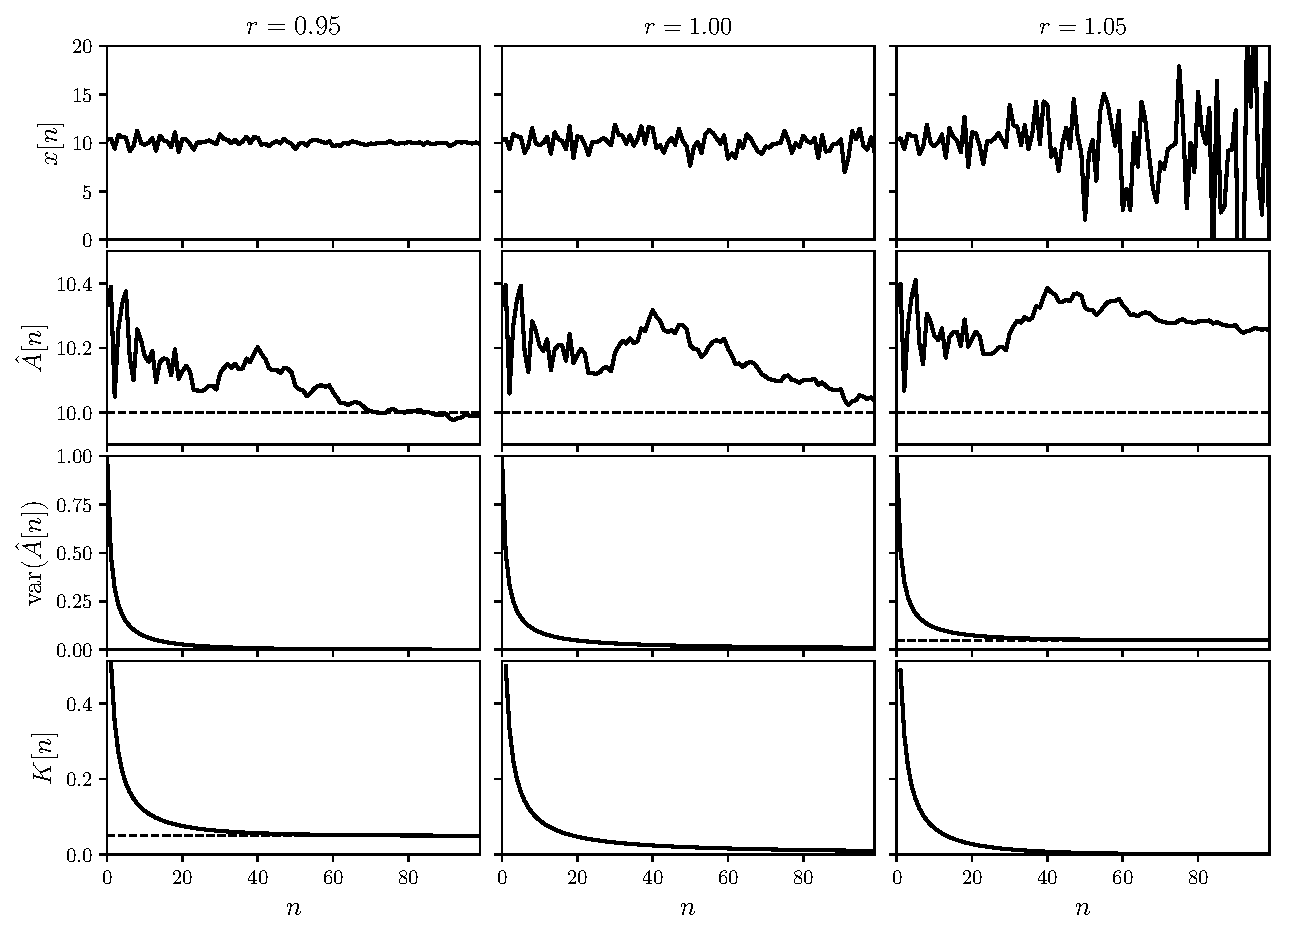
\includegraphics[width=\textwidth]{figuras/problem_8_22.pdf}
\caption{\label{fig:problem_8_22} Estimador LSE secuencial de \(A\), con \(x[n]=A+w[n]\). La varianza del ruido \(w[n]\) es \(r^n\). Se muestran los resultados para \(r=0.95,\,1,\,1.05\). Con \(r>1\), la varianza del estimador no tiende a cero, por lo que la estimación no alcanza nunca el valor correcto.}
\end{center}
\end{figure}
Como se dedujo en el problema anterior, cuando \(0<r<1\), la varianza del ruido decrece y la varianza del estimador tiene a cero. Esto implica que la estimación es perfecta con \(N\to\infty\). Además, \(K[N]\to 1-r\) con \(N\to\infty\). En el caso en que \(r>1\), la potencia del ruido crece. La ganancia tiene a cero rápidamente, lo que significa que las muestras se toman cada vez menos en cuenta cuando \(N\) crece. Esto puede verse como emplear un número finito de muestras para calcular el estimador. Por esta razón, la varianza del estimador no tiende a cero.


\subsection{Problema 23}\label{sec:problem_8_23}

En este problema se examina la inicialización del LSE secuencial. Asúmase que se elige \(\hat{\thetabf}[-1]\) y \(\bm{\Sigma}[-1]=\alpha\I\) para inicializar el LSE. Se mostrará que si \(\alpha\to\infty\), el estimador  LSE por lotes
\begin{align*}
 \hat{\thetabf}_B[n]&=(\Hbf^T[n]\C^{-1}[n]\Hbf[n])^{-1}\Hbf^T[n]\C^{-1}[n]\x[n]\\
  &=\left(\sum_{k=0}^{n}\frac{1}{\sigma_k^2}\h[h]\h^T[k]\right)^{-1}\left(\sum_{k=0}^{n}\frac{1}{\sigma_k^2}x[h]\h[k]\right)
\end{align*}
es idéntico al estimador secuencial para \(n\geq p\). Primero, asúmase que los vectores de observación \(\{\h[-p],\,\h[-(p-1)],\,\dots,\,\h[-1]\}\) y las varianzas del ruido \(\{\sigma^2_{-p},\,\sigma^2_{-(p-1)},\,\dots,\,\sigma^2_{-1}\}\) existen, de forma que para el LSE y matriz de covarianza inicial elegidos es posible calcular el LSE por lotes. Por lo tanto,
\[
 \hat{\thetabf}[-1]=\hat{\thetabf}_B[-1]=(\Hbf^T[-1]\C^{-1}[-1]\Hbf[-1])^{-1}\Hbf^T[-1]\C^{-1}[-1]\x[-1]
\]
y
\[
 \bm{\Sigma}[-1]=(\Hbf^T[-1]\C^{-1}[-1]\Hbf[-1])^{-1}
\]
donde
\begin{align*}
 \Hbf[-1]&=
 \begin{bmatrix}
  \h^T[-p]\\
  \h^T[-(p-1)]\\
  \vdots\\
  \h^T[-1]
 \end{bmatrix}\\
 \C[-1]&=\operatorname{diag}\left(\sigma^2_{-p},\,\sigma^2_{-(p-1)},\,\dots,\,\sigma^2_{-1}\right).
\end{align*}
De esta forma, se puede ver al estimador inicial del LSE secuencial como el resultado de aplicar un estimador por lotes con los vectores de observación iniciales. Debido a que el LSE secuencial inicializado mediante el estimador por lotes es idéntico al estimador por lotes empleando todos los vectores de observación, se cumple que el LSE secuencial con las condiciones iniciales asumidas es
\begin{equation}\label{eq:ls_sequential_estimator_tmp}
 \hat{\thetabf}_S[n]=\left(\sum_{k=-p}^{n}\frac{1}{\sigma_k^2}\h[h]\h^T[k]\right)^{-1}\left(\sum_{k=-p}^{n}\frac{1}{\sigma_k^2}x[h]\h[k]\right).
\end{equation}
Mostrar que esto puede reescribirse como
\[
 \hat{\thetabf}_S[n]=\left(\bm{\Sigma}^{-1}[-1]+\sum_{k=0}^{n}\frac{1}{\sigma_k^2}\h[h]\h^T[k]\right)^{-1}\left(\bm{\Sigma}^{-1}[-1]+\sum_{k=0}^{n}\frac{1}{\sigma_k^2}x[h]\h[k]\right).
\]
Luego, examinar que ocurre cuando \(\alpha\to\infty\) para \(0\leq n\leq p-1\) y para \(n\geq p\),

\paragraph{Solución} Las matrices de observación y de covarianza del ruido del estimador por lotes con las condiciones iniciales indicadas son
\begin{align*}
 \Hbf[n]&=
 \begin{bmatrix}
  \h^T[-p]\\
  \vdots\\
  \h^T[-1]\\
  \h^T[0]\\
  \vdots\\
  \h^T[n]
 \end{bmatrix}\\
 \C[n]&=\operatorname{diag}\left(\sigma^2_{-p},\,\dots,\,\sigma^2_{-1},\,\sigma^2_0,\,\dots,\,\sigma^2_n\right).
\end{align*}
y por lo tanto, al aplicar la ecuación \ref{eq:ls_sequential_estimator_batch} se observa que efectivamente el estimador secuencial está dado por la ecuación \ref{eq:ls_sequential_estimator_tmp}. Esta ecuación se puede escribir como
\[
 \hat{\thetabf}_S[n]=\left(\sum_{k=-p}^{-1}\frac{1}{\sigma_k^2}\h[h]\h^T[k]+\sum_{k=0}^{n}\frac{1}{\sigma_k^2}\h[h]\h^T[k]\right)^{-1}\left(\sum_{k=-p}^{-1}\frac{1}{\sigma_k^2}x[h]\h[k]+\sum_{k=0}^{n}\frac{1}{\sigma_k^2}x[h]\h[k]\right).
\]
Por otro lado, se cumple que
\begin{align*}
 \hat{\thetabf}[-1]&=(\Hbf^T[-1]\C^{-1}[-1]\Hbf[-1])^{-1}\Hbf^T[-1]\C^{-1}[-1]\x[-1]\\
   &=\bm{\Sigma}[-1]\Hbf^T[-1]\C^{-1}[-1]\x[-1],
\end{align*}
y por lo tanto, 
\begin{align*}
 \bm{\Sigma}^{-1}[-1]\hat{\thetabf}[-1]&=\Hbf^T[-1]\C^{-1}[-1]\x[-1]\\
   &=\sum_{k=-p}^{-1}\frac{1}{\sigma_k^2}x[h]\h[k].
\end{align*}
Además,
\begin{align*}
 \bm{\Sigma}^{-1}[-1]&=\Hbf^T[-1]\C^{-1}[-1]\Hbf[-1]\\
   &=\sum_{k=-p}^{-1}\frac{1}{\sigma_k^2}\h[h]\h^T[k].
\end{align*}
Combinando estos resultados, se obtiene que
\[
 \hat{\thetabf}_S[n]=\left(\bm{\Sigma}^{-1}[-1]+\sum_{k=0}^{n}\frac{1}{\sigma_k^2}\h[h]\h^T[k]\right)^{-1}\left(\bm{\Sigma}^{-1}[-1] \hat{\thetabf}[-1]+\sum_{k=0}^{n}\frac{1}{\sigma_k^2}x[h]\h[k]\right),
\]
que es lo que se quería mostrar. Asúmase ahora que se elige \(\bm{\Sigma}[-1]=\alpha\I\) para inicializar el LSE. Si \(\alpha\to\infty\),
\[
 \bm{\Sigma}^{-1}[-1]=\frac{\I}{\alpha}\to\mathbf{0}
\]
y por lo tanto,
\[
 \left(\bm{\Sigma}^{-1}[-1]+\sum_{k=0}^{n}\frac{1}{\sigma_k^2}\h[h]\h^T[k]\right)^{-1}\underset{\alpha\to\infty}{\longrightarrow}\left(\sum_{k=0}^{n}\frac{1}{\sigma_k^2}\h[h]\h^T[k]\right)^{-1}
 =\left(\Hbf^T[n]\C^{-1}[n]\Hbf[n]\right)^{-1}.
\]
\(\Hbf[n]\) es una matriz \((n+1)\times p\). En el caso en que \(n+1<p\) se cumple que
\[
 \operatorname{rank}(\Hbf[n])\leq n+1<p.
\]
Por lo tanto,
\[
  \operatorname{rank}\left(\Hbf^T[n]\C^{-1}[n]\Hbf[n]\right)\overset{(a)}{=}\operatorname{rank}\left(\Hbf^T[n]\Hbf[n]\right)\overset{(b)}{=}\operatorname{rank}(\Hbf[n])\leq n+1<p
\]
donde en \((a)\) se consideró que \(\C^{-1}[n]\) es una matriz diagonal y por lo tanto, de rango completo, y en \((b)\) que \(\operatorname{rank}(\A^T\A)=\operatorname{rank}(\A)\), como se explica en el apéndice \ref{ap:lineal_algebra_basics}. Teniendo en cuenta que \(\Hbf^T[n]\C^{-1}[n]\Hbf[n]\) es una matriz \(p\times p\) con \(\operatorname{rank}\left(\Hbf^T[n]\C^{-1}[n]\Hbf[n]\right)<p\), se concluye que no es invertible y por lo tanto, no es posible tomar \(\alpha\to\infty\) si \(n+1<p\). En el caso en que \(n+1\geq p\), \(\Hbf^T[n]\C^{-1}[n]\Hbf[n]\) es invertible (asumiendo que las \(p\) columnas son linealmente independientes) y se cumple que
\[
 \hat{\thetabf}_S[n]\underset{\alpha\to\infty}{\longrightarrow}\left(\sum_{k=0}^{n}\frac{1}{\sigma_k^2}\h[h]\h^T[k]\right)^{-1}\left(\sum_{k=0}^{n}\frac{1}{\sigma_k^2}x[h]\h[k]\right)=\hat{\thetabf}_B[n],
\]
que es lo que se quería mostrar.

\subsection{Problema 24}\label{sec:problem_8_24}

En el ejemplo de la sección \ref{sec:ls_constrained} de la estimación de una señal restringida, determinar \(\hat{\s}_c\) primero proyectando \(\x\) en el subespacio generado por \(\h_1\) y \(\h_2\) para producir \(\hat{\s}\) y luego proyectando \(\hat{\s}\) en el subespacio restringido.

\paragraph{Solución} La proyección ortogonal de \(\x\) sobre el subespacio generado por las columnas de \(\Hbf\) es
\[
 \hat{\s}=\Hbf(\Hbf^T\Hbf)^{-1}\Hbf^T\x,\qquad\qquad\textrm{con}\qquad\qquad
 \Hbf=
 \begin{bmatrix}
  1 & 0\\ 0 & 1\\ 0 & 0
 \end{bmatrix}.
\]
Considerando que
\[
 \Hbf^T\Hbf=
 \begin{bmatrix}
  1 & 0\\ 0 & 1
 \end{bmatrix}
 =\I\qquad\qquad\textrm{y}\qquad\qquad
 \Hbf\Hbf^T=
 \begin{bmatrix}
  1 & 0 & 0\\ 0 & 1 & 0\\ 0 & 0 & 0
 \end{bmatrix},
\]
se obtiene que
\[
 \hat{\s}=
 \begin{bmatrix}
  x[0] \\ x[1] \\ 0
 \end{bmatrix}.
\]
Como se discutió en el ejemplo, el subespacio restringido es el generado por el vector
\[
 \h_c=
 \begin{bmatrix}
  1 \\ 1 \\ 0
 \end{bmatrix}
\]
y la proyección ortogonal de \(\hat{\s}\) sobre este subespacio es
\[
 \hat{\s}_c=\h_c(\h_c^T\h_c)^{-1}\h_c^T\hat{\s}
\]
Considerando que
\[
 \h_c^T\h_c=2\qquad\qquad\textrm{y}\qquad\qquad
 \h_c\h_c^T=
 \begin{bmatrix}
  1 & 1 & 0\\ 1 & 1 & 0\\ 0 & 0 & 0
 \end{bmatrix},
\]
se obtiene que
\[
 \hat{\s}_c=\frac{1}{2}
 \begin{bmatrix}
  x[0]+x[1]\\
  x[0]+x[1]\\
  0
 \end{bmatrix},
\]
que coincide con el resultado de la sección \ref{sec:ls_constrained}.

\subsection{Problema 25}

Si el modelo de la señal es
\[
 s[n]=A+B(-1)^n,\qquad n=0,\,\dots,\,N-1,
\]
con \(N\) par, encontrar el LSE de \(\thetabf=[A\,B]^T\). Asumiendo que \(A=B\), repetir el problema empleando el enfoque de LS restringidos. Comparar los resultados.

\paragraph{Solución} En notación matricial, el modelo de la señal es
\[
 \s=\Hbf\thetabf,\qquad\qquad\textrm{con}\qquad\qquad
 \Hbf=
 \begin{bmatrix}
  1 & 1\\1 & -1\\1 & 1\\ \vdots & \vdots\\1 & -1 
 \end{bmatrix}.
\]
El LSE es
\begin{align*}
 \hat{\thetabf}&=(\Hbf^T\Hbf)^{-1}\Hbf^T\x\\
  &=\frac{1}{N}\Hbf^T\x
\end{align*}
donde se tuvo en cuenta que
\[
 \Hbf^T\Hbf=
 \begin{bmatrix}
  N & 0\\ 0 & N
 \end{bmatrix}
 =N\I,
\]
resultando en
\[
 \hat{\thetabf}=\frac{1}{N}
 \renewcommand*{\arraystretch}{2.8}
 \begin{bmatrix}
  \displaystyle\sum_{n=0}^{N-1}x[n]\\
  \displaystyle\sum_{n=0}^{N-1}(-1)^nx[n]
 \end{bmatrix}.
\]
Asumiendo que \(A=B\), la restricción en la forma de la ecuación \ref{eq:ls_constrained_constrains} es
\[
 \begin{bmatrix}
  1 & -1
 \end{bmatrix}
 \begin{bmatrix}
  A\\B
 \end{bmatrix}
 =0,
\]
por lo que \(\A=[1\,-1]\) y \(\bbf=0\).
El estimador restringido, que está dado por la ecuación \ref{eq:ls_constrained_estimator} es
\begin{align*}
 \hat{\thetabf}_c&=\hat{\thetabf}-(\Hbf^T\Hbf)^{-1}\A^T[\A(\Hbf^T\Hbf)^{-1}\A^T]^{-1}(\A\hat{\thetabf}-\bbf)\\
   &\overset{(a)}{=}\hat{\thetabf}-\frac{1}{N}\A^T\left(\frac{\A\A^T}{N}\right)^{-1}\A\hat{\thetabf}\\
   &=[\I-\A^T(\A\A^T)^{-1}\A]\hat{\thetabf},
\end{align*}
donde en \((a)\) se consideró que \(\Hbf^T\Hbf=N\I\). Teniendo en cuenta que 
\[
 \I-\A^T(\A\A^T)^{-1}\A=
 \frac{1}{2}
   \begin{bmatrix}
    1 & 1\\ 1 & 1
   \end{bmatrix},
\]
como se calculó en la sección \ref{sec:ls_constrained}, y sustituyendo \(\hat{\thetabf}\) se obtiene que
\begin{align*}
 \hat{\thetabf}_c&=\frac{1}{2N}
  \renewcommand*{\arraystretch}{2.8}
 \begin{bmatrix}
  \displaystyle\sum_{n=0}^{N-1}x[n]+\sum_{n=0}^{N-1}(-1)^nx[n]\\
  \displaystyle\sum_{n=0}^{N-1}x[n]+\sum_{n=0}^{N-1}(-1)^nx[n]
 \end{bmatrix}.
\end{align*}
De esta forma,
\begin{align*}
 \hat{A}_c=\hat{B}_c&=\frac{1}{2N}\sum_{n=0}^{N-1}[x[n]+(-1)^nx[n]]\\
  &=\frac{1}{2N}\sum_{n=0}^{N-1}x[n][1+(-1)^n]\\
  &=\frac{1}{2N}\sum_{\substack{n=0 \\ n\textrm{ par}}}^{N-1}2x[n]\\
  &=\frac{1}{N}\sum_{n=0}^{\frac{N}{2}-1}x[2n]\\
  &=\frac{1}{2}\times\frac{2}{N}\sum_{n=0}^{\frac{N}{2}-1}x[2n],
\end{align*}
es decir
\[
 \hat{A}_c=\frac{\bar{x'}}{2},\qquad\textrm{con}\qquad\x'=[x[0]\,x[2]\,\dots\,x[N-2]].
\]
Esto tiene sentido, ya que el modelo de señal con \(A=B\) es
\[
 s[n]=A+(-1)^nA=2A
 \left\{
 \begin{array}{rl}
  2A, & n\textrm{ par}\\
  0, & n\textrm{ impar},
 \end{array}\right.
\]
y el LSE restringido \(\hat{A}_c\) es el promedio de las muestras pares de \(x[n]\) dividido 2.

\subsection{Problema 26}\label{sec:problem_8_26}

Considérese la minimización de \(h(\theta)\) respecto a \(\theta\) y asúmase que
\[
 \hat{\theta}=\argmin_{\theta}h(\theta).
\]
Sea \(\alpha=g(\theta)\), donde \(g\) es una función uno a uno. Probar que si \(\hat{\alpha}\) minimiza \(h(g^{-1}(\hat{\alpha}))\), se cumple que \(\hat{\theta}=g^{-1}(\hat{\alpha})\).

\paragraph{Solución} Por hipótesis, se cumple que \(\hat{\alpha}\) minimiza \(h(g^{-1}(\hat{\alpha}))\), lo que implica que
\[
 \frac{dh(g^{-1}(\alpha))}{d\alpha}\bigg|_{\alpha=\hat{\alpha}}=0.
\]
Aplicando la regla de la cadena de la diferenciación, se tiene que
\[
 \frac{dh(g^{-1}(\alpha))}{d\alpha}=h'(g^{-1}(\alpha))\frac{dg^{-1}(\alpha)}{d\alpha}
 \overset{(a)}{=}h'(g^{-1}(\alpha))\frac{1}{g'(g^{-1}(\alpha))}
\]
donde en \((a)\) se consideró que la derivada de una función inversa está dada por\footnote{Ver \url{https://en.wikipedia.org/wiki/Inverse_functions_and_differentiation}.} \(\left[f^{{-1}}\right]'(a)=1/f'\left(f^{-1}(a)\right)\). Por lo tanto, se cumple que
\[
 h'(g^{-1}(\alpha))\frac{1}{g'(g^{-1}(\alpha))}\bigg|_{\alpha=\hat{\alpha}}=0
\]
Considerando que \(g\) es una función inyectiva, se cumple que \(g'(\theta)\) es estrictamente positiva o negativa para todo \(\theta\), por lo que la condición resulta en
\[
 h'(g^{-1}(\hat{\alpha}))=0.
\]
Como
\[
 \hat{\theta}=\argmin_{\theta}h(\theta)\qquad\Leftrightarrow\qquad h'(\hat{\theta})=0,
\]
se concluye que
\[
 \hat{\theta}=g^{-1}(\hat{\alpha}).
\]

Una forma simple de ver lo mismo, es partiendo de que por hipótesis se cumple que
\[
 h(g^{-1}(\hat{\alpha}))\leq h(g^{-1}(\alpha))\qquad\forall\alpha,
\]
y por lo tanto
\[
 h(\theta_0)\leq h(\theta)\qquad\forall\theta,\qquad\textrm{con }\theta_0=g^{-1}(\hat{\alpha}).
\]
Pero como \(\theta_0\) minimiza \(h(\theta)\), \(\hat{\theta}=\theta_0\), resultando en que
\[
 \hat{\theta}=g^{-1}(\hat{\alpha}).
\]

\subsection{Problema 27}

Sean los datos observados
\[
 x[n]=e^\theta+w[n],\qquad n=0,\,\dots,\,N-1.
\]
Determinar una iteración de Newton-Raphson para encontrar el LSE de \(\theta\). ¿Es posible evitar la optimización no lineal y encontrar el LSE analíticamente?

\paragraph{Solución} En este caso, el modelo de señal es \(s[n]=e^\theta\), por lo que la función de error a minimizar es
\[
 J(\theta)=\sum_{n=0}^{N-1}(x[n]-e^\theta)^2.
\]
Diferenciando respecto al parámetro, se obtiene que la condición necesaria es
\[
 \frac{\partial J}{\partial\theta}=-2\sum_{n=0}^{N-1}(x[n]-e^\theta)e^\theta=0
 \quad\Rightarrow\quad \sum_{n=0}^{N-1}(x[n]-e^{\hat{\theta}})=0
 \quad\Rightarrow\quad Ne^{\hat{\theta}}=\sum_{n=0}^{N-1}x[n]
 \quad\Rightarrow\quad e^{\hat{\theta}}=\bar{x}
\]
resultando en que el LSE es
\[
 \hat{\theta}=\ln\bar{x}.
\]
Notar que si se realiza la transformación del parámetro \(\alpha=g(\theta)=e^\theta\), el problema es lineal y el estimador LSE de \(\alpha\) es \(\hat{\alpha}=\bar{x}\). Como la transformación \(g\) es biyectiva, el estimador LSE de \(\theta\) es \(\hat{\theta}=g^{-1}(\hat{\alpha})=\ln\hat{\alpha}\), como se mostró en el problema de la sección \ref{sec:problem_8_26}. Si bien el problema no es lineal, se encontró un expresión analítica para el estimador. 

Para encontrar una solución iterativa empleando el algoritmo de Newton-Raphson, que está dado por la ecuación \ref{eq:ls_nlls_deduction_iteration_tmp}, se parte de que la función a encontrar la raíz es
\[
 g(\theta)=e^\theta\sum_{n=0}^{N-1}(x[n]-e^\theta)=e^\theta\left(\sum_{n=0}^{N-1}x[n]-Ne^\theta\right).
\]
Teniendo en cuenta que la derivada es
\[
 g'(\theta)=e^\theta\left(\sum_{n=0}^{N-1}x[n]-Ne^\theta\right)-e^\theta Ne^\theta
  =e^\theta\left(\sum_{n=0}^{N-1}x[n]-2Ne^\theta\right).
\]
la iteración de Newton-Raphson queda
\begin{align*}
 \theta_{k+1}&=\theta_{k}-\frac{g(\theta_k)}{g'(\theta_k)}\\
  &=\theta_{k}-\dfrac{\displaystyle e^{\theta_k}\left(\sum_{n=0}^{N-1}x[n]-Ne^{\theta_k}\right)}{\displaystyle e^{\theta_k}\left(\sum_{n=0}^{N-1}x[n]-2Ne^{\theta_k}\right)}\\
\end{align*}
resultando en
\[
 \theta_{k+1}=\theta_{k}+\frac{\bar{x}-e^{\theta_k}}{2e^{\theta_k}-\bar{x}}.
\]
También podría haberse considerado como función a resolver a 
\[
g(\theta)=\sum_{n=0}^{N-1}(x[n]-e^\theta),
\]
resultando en una iteración distinta. El mismo resultado se obtiene empleando directamente la ecuación \ref{eq:ls_nlls_estimator_nr} de la iteración de Newton-Raphson para el LSE no lineal genérico. Como en este caso \(s[n]=e^\theta\), o \(\s=e^\theta\mathbf{1}\), se tiene que
\[
 \frac{\partial s[i]}{\partial\theta}=e^\theta,\qquad i=0,\,\dots,\,N-1\qquad\qquad\Rightarrow\qquad\qquad\Hbf(\theta)=e^\theta\mathbf{1}
\]
y
\[
 \frac{\partial^2 s[n]}{\partial\theta^2}=e^\theta,\qquad n=0,\,\dots,\,N-1\qquad\qquad\Rightarrow\qquad\qquad\G_n(\theta)=e^\theta,
\]
la iteración de Newton-Raphson es
\begin{align*}
 \theta_{k+1}&=\theta_{k}+\left(\Hbf^T(\theta_k)\Hbf(\theta_k)-\sum_{n=0}^{N-1}\G_n(\theta_k)(x[n]-s[n])\right)^{-1}\Hbf^T(\theta_k)(\x-\s(\theta_k))\\
  &=\theta_{k}+\left(e^{2\theta_k}\mathbf{1}^T\mathbf{1}-e^{\theta_k}\sum_{n=0}^{N-1}(x[n]-e^{\theta_k})\right)^{-1}e^{\theta_k}\mathbf{1}^T(\x-e^{\theta_k}\mathbf{1})\\
  &=\theta_{k}+\frac{\displaystyle e^{\theta_k}\sum_{n=0}^{N-1}(x[n]-e^{\theta_k})}{\displaystyle e^{\theta_k}\left[Ne^{\theta_k}-\sum_{n=0}^{N-1}(x[n]-e^{\theta_k})\right]}\\
  &=\theta_{k}+\frac{\displaystyle \sum_{n=0}^{N-1}x[n]-Ne^{\theta_k}}{\displaystyle 2Ne^{\theta_k}-\sum_{n=0}^{N-1}x[n]}\\
  &=\theta_{k}+\frac{\bar{x}-e^{\theta_k}}{2e^{\theta_k}-\bar{x}}.
\end{align*}

\subsection{Problema 28}\label{sec:problem_8_28}

En el ejemplo de la sección \ref{sec:ls_example_digital_filter_design} el LSE verdadero debe minimizar
\[
 J=\sum_{n=0}^{N-1}(h_d[n]-h[n])^2.
\]
En este problema se deducen las ecuaciones que hay que optimizar para encontrar el LSE verdadero. Se asume que \(p=q+1\). Primero, mostrar que el modelo de señal puede escribirse como
\[
 \s=
 \begin{bmatrix}
  h[0]\\h[1]\\\vdots\\h[N-1]
 \end{bmatrix}
 =
 \underbrace{
 \begin{bmatrix}
  g[0] & 0 & \dots & 0\\
  g[1] & g[0] & \dots & 0\\
  \vdots & \vdots & \ddots & \vdots\\
  g[q] & g[q-1] & \dots & g[0]\\
  g[q+1] & g[q] & \dots & g[1]\\
  \vdots & \vdots &  & \vdots\\
  g[N-1] & g[N-2] & \dots & g[N-1-q]
 \end{bmatrix}}_{\displaystyle \G}
 \underbrace{\vphantom{\begin{bmatrix}g[0]\\g[0]\\\vdots\\g[0]\\g[0]\\\vdots\\g[0]\end{bmatrix}}
 \begin{bmatrix}
  b[0]\\b[1]\\\vdots\\b[q]
 \end{bmatrix}}_{\displaystyle \bbf}
\]
donde
\[
 g[n]=\mathcal{Z}^{-1}\left\{\frac{1}{\mathcal{A}(z)}\right\}
\]
y la matriz \(\G\) tiene dimensiones \(N\times(q+1)\). Si \(\x=[h_d[0]\,h_d[1]\,\dots\,h_d[N-1]]^T\) mostrar que
\[
 J(\abf,\,\hat{\bbf})=\x^T(\I-\G(\G^T\G)^{-1}\G^T)\x
\]
donde \(\hat{\bbf}\) es el LSE de \(\bbf\) para un \(\abf\) dado. Finalmente, probar que
\begin{equation}\label{eq:ls_problem_8_28_proy_matrix}
 \I-\G(\G^T\G)^{-1}\G^T=\A(\A^T\A)^{-1}\A^T
\end{equation}
donde \(\A^T\) es la matriz de dimensiones \((N-q-1)\times N=(N-p)\times N\)
\begin{equation}\label{eq:ls_problem_8_28_A_matrix}
 \A^T=
 \begin{bmatrix}
  a[p] & a[p-1] & \dots & 1    & 0 & 0 & \dots & 0\\
  0    & a[p]   & \dots & a[1] & 1 & 0 & \dots & 0\\
  \vdots & \vdots &     & \vdots& \vdots& \vdots & & \vdots\\
  0 & 0 & \dots & 0 & a[p] & a[p-1] & \dots & 1\\
 \end{bmatrix}. 
\end{equation}
Por lo tanto, el LSE de \(\abf\) se obtiene minimizando
\[
 \x^T\A(\A^T\A)^{-1}\A^T\x,
\]
y luego que es encontrado empleando una técnica de optimización no lineal, se tiene que
\begin{align*}
 \hat{\bbf}&=(\G^T\G)^{-1}\G^T\x\\ 
 \hat{\s}&=(\I-\A(\A^T\A)^{-1}\A^T)\x,
\end{align*}
donde los elementos de \(\A\) son reemplazados por el LSE de \(\abf\). Notar que este problema es un ejemplo de un problema LS no lineal separable. Sugerencia: para probar la identidad \ref{eq:ls_problem_8_28_proy_matrix} considerar \(\Lbf=[\A\,\G]\), la cual es invertible debido a que es de rango completo y calcular
\[
 \Lbf(\Lbf^T\Lbf)^{-1}\Lbf^T=\I.
\]
También se necesita observar que \(\A^T\G=\mathbf{0}\), que surge de que \(a[n]*g[n]=\delta[n]\).

\paragraph{Solución} Este problema se analiza en la sección 9.18 de \cite{scharf1991statistical}. Se comenzará deduciendo el modelo de la señal. El sistema es un modelo ARMA con función de transferencia
\[
 \mathcal{H}(z)=\frac{\mathcal{B}(z)}{\mathcal{A}(z)}=\frac{b[0]+b[1]z^{-1}+\dots+b[q]z^{-q}}{1+a[1]z^{-1}+\dots+a[p]z^{-p}}
\]
con \(p=q+1\). Aplicando la transformada \(z\) inversa se obtiene la respuesta al impulso, y es
\begin{align*}
 h[n]&=\mathcal{Z}^{-1}\{\mathcal{H}(z)\}\\
  &=\mathcal{Z}^{-1}\left\{\frac{b[0]+b[1]z^{-1}+\dots+b[q]z^{-q}}{\mathcal{A}(z)}\right\}\\
  &=b[0]\mathcal{Z}^{-1}\left\{\frac{1}{\mathcal{A}(z)}\right\}+b[1]\mathcal{Z}^{-1}\left\{\frac{z^{-1}}{\mathcal{A}(z)}\right\}+\dots+b[q]\mathcal{Z}^{-1}\left\{\frac{z^{-q}}{\mathcal{A}(z)}\right\}\\
  &=b[0]g[n]+b[1]g[n-1]+\dots+b[q]g[n-q]\\
  &=\sum_{k=0}^{q}b[k]g[n-k],
\end{align*}
donde se definió
\[
 g[n]=\mathcal{Z}^{-1}\left\{\frac{1}{\mathcal{A}(z)}\right\}
\]
y se empleó que \(\mathcal{Z}^{-1}\{z^{-k}\mathcal{G}(z)\}=g[n-k]\). Por lo tanto, se tiene que
\[
 \begin{array}{ccccccccc}
  h[0]&=&b[0]h[0]& &&&&&\\
  h[1]&=&b[0]g[1]&+&g[1]g[0]& &&&\\
  \vdots & & \vdots & & \vdots &&&&\\
  h[q]&=&b[0]g[q]&+&b[1]g[q-1]&+&\dots&+&b[q]g[0]\\
  \vdots & & \vdots & & \vdots &&&& \vdots \\
  h[N-1]&=&b[0]g[N-1]&+&b[1]g[N-2]&+&\dots&+&b[q]g[N-1-q]
 \end{array}
\]
que en notación matricial se expresa como
\[
 \s=
 \begin{bmatrix}
  h[0]\\h[1]\\\vdots\\h[N-1]
 \end{bmatrix}
 =
 \underbrace{
 \begin{bmatrix}
  g[0] & 0 & \dots & 0\\
  g[1] & g[0] & \dots & 0\\
  \vdots & \vdots & \ddots & \vdots\\
  g[q] & g[q-1] & \dots & g[0]\\
  g[q+1] & g[q] & \dots & g[1]\\
  \vdots & \vdots &  & \vdots\\
  g[N-1] & g[N-2] & \dots & g[N-1-q]
 \end{bmatrix}}_{\displaystyle \G}
 \underbrace{\vphantom{\begin{bmatrix}g[0]\\g[0]\\\vdots\\g[0]\\g[0]\\\vdots\\g[0]\end{bmatrix}}
 \begin{bmatrix}
  b[0]\\b[1]\\\vdots\\b[q]
 \end{bmatrix}}_{\displaystyle \bbf},
\]
donde la matriz \(\G\) tiene dimensiones \(N\times(q+1)\) o \(N\times p\) y depende del parámetro \(\abf\). Se observa que es un modelo lineal en el parámetro \(\bbf\). Si las observaciones son \(\x=[h_d[0]\,h_d[1]\,\dots\,h_d[N-1]]^T\), el error LS es
\begin{align*}
 J(\abf,\,\bbf)&=\sum_{n=0}^{N-1}(h_d[n]-h[n])^2\\
  &=(\x-\s)^T(\x-\s)\\
  &=(\x-\G(\abf)\bbf)^T(\x-\G(\abf)\bbf),
\end{align*}
donde por única vez se hizo explícita la dependencia de la matriz \(\G\) con el parámetro \(\abf\). Por tratarse de un problema LS lineal en \(\bbf\), el LSE \(\hat{\bbf}\) que minimiza el error para un \(\abf\) dado es
\[
 \hat{\bbf}=(\G^T\G)^{-1}\G^T\x
\]
y el error mínimo es
\begin{align*}
 J(\abf,\,\hat{\bbf})&=(\x-\G\hat{\bbf})^T(\x-\G\hat{\bbf})\\
  &=(\x-\G(\G^T\G)^{-1}\G^T\x)^T(\x-\G(\G^T\G)^{-1}\G^T\x)\\
  &=\x^T(\I-\G(\G^T\G)^{-1}\G^T)(\I-\G(\G^T\G)^{-1}\G^T)\x,
\end{align*}
donde se consideró que la matriz de proyección \(\I-\G(\G^T\G)^{-1}\G^T\) es simétrica y teniendo en cuenta que además es idempotente (ver los problemas de las secciones \ref{sec:problem_8_11} y \ref{sec:problem_8_12}), resulta en
\[
 J(\abf,\,\hat{\bbf})=\x^T(\I-\G(\G^T\G)^{-1}\G^T)\x.
\]
Para probar la identidad de la ecuación \ref{eq:ls_problem_8_28_proy_matrix}, se necesita primero observar que por definición
\[
 \mathcal{G}(z)=\frac{1}{\mathcal{A}(z)}=\frac{1}{1+a[1]z^{-1}+\dots+a[p]z^{-p}}
 \qquad\Rightarrow\qquad
 \mathcal{G}(z)(1+a[1]z^{-1}+\dots+a[p]z^{-p})=1,
\]
y aplicando la transformada \(z\) inversa, se obtiene que
\begin{equation}\label{eq:ls_problem_8_28_gn}
 g[n]+a[1]g[n-1]+\dots+a[p]g[n-p]=\delta[n]\qquad\quad\textrm{o}\qquad\quad
 \sum_{k=0}^pa[k]g[n-k]=\delta[n].
\end{equation}
Definiendo \(a[n]=0\) en \(n<0\) y \(n>p\) y \(g[n]=0\) en \(n<0\), la expresión se puede escribir como
\begin{equation}\label{eq:ls_problem_8_28_a_conv_g}
 \sum_{k=-\infty}^\infty a[k]g[n-k]=\delta[n]\qquad\qquad\textrm{o}\qquad\qquad
 (a*g)[n]=\delta[n].
\end{equation}
Este resultado se puede obtener directamente empleando la propiedad de convolución de la tranformada z,
\[
 \mathcal{A}(z)\mathcal{G}(z)=1\qquad\overset{\mathcal{Z}^{-1}}{\longrightarrow}\qquad(a*g)[n]=\delta[n].
\]
Continuando con la prueba de \ref{eq:ls_problem_8_28_proy_matrix}, se considera la matriz \(\Lbf=[\A\,\G]\), donde \(\A\) es la matriz de la ecuación \ref{eq:ls_problem_8_28_A_matrix}. Como la matriz \(\A\) tiene dimensiones \(N\times (N-p)\) y la matriz \(\G\) tiene dimensiones \(N\times p\), la matriz \(\Lbf\) es cuadrada de dimensiones \(N\times N\). Se verá que además que es de rango completo. Para hacerlo, se parte observando que debido a su estructura, las matrices \(\A\) y \(\G\) son de rango completo, con rangos \(N-p\) y \(p\) respectivamente. Si se prueba que las columnas de \(\A\) son linealmente independientes a las columnas de \(\G\) se concluye que \(\Lbf\) tiene \(N\) columnas linealmente independientes y por lo tanto, es de rango completo \(N\). Se mostrará que las matrices \(\A\) y \(\G\) son ortogonales entre si, o \(\A^T\G=\mathbf{0}\), lo que implica que sus columnas son linealmente independientes. La columna \(i\)-ésima de \(\A\), que es la fila \(i\)-ésima de \(\A^T\), con \(0\leq i\leq N-p-1\), y la columna \(j\)-ésima de \(\G\), con \(0\leq j\leq p-1\), son respectivamente
\[
\begin{array}{ccrcccccccccccl}
 [\A]_i & = & [ & 0 & \dots & 0 & 0 & a[p] & a[p-1] & \dots & a[0] & 0 & \dots & 0 & ]^T\\
  & & & {\scriptstyle k=0} & & & & {\scriptstyle k=i} & & & {\scriptstyle k=i+p} & & & {\scriptstyle k=N-1}\\
 \left[\G\right]_j & = & [ & 0 & \dots & 0 & g[0] & g[1] & \dots & \dots & \dots & \dots & \dots & g[N-1-j] & ]^T.\\
  & & & {\scriptstyle k=0} & & & {\scriptstyle k=j} & & & & & & & {\scriptstyle k=N-1}
\end{array}
\]
Por lo tanto, el elemento \((k,\,i)\) de \(\A\) y el elemento \((k,\,j)\) de \(\G\) son respectivamente
\[
 \begin{array}{llllc}
  [\A]_{ki}&=&a[p+i-k] &\textrm{con }a[n]=0\textrm{ en }n<0\textrm{ y }n>p\\
  \left[\G\right]_{kj}&=&g[k-j] &\textrm{con }g[n]=0\textrm{ en }n<0.
 \end{array}
\]
En la figura \ref{fig:problem_8_28_an} se ilustra gráficamente los elementos de una columna de la matriz \(\A\), los cuales son una versión invertida temporalmente y desplazada de \(a[n]\). 
\begin{figure}[!htb]
\begin{center}
\includegraphics[width=0.9\textwidth]{figuras/problem_8_28_an.pdf}
\caption{\label{fig:problem_8_28_an} Columna \(i\)-ésima de la matriz \(\A\). Se trata de la secuencia \(a[p+i-k]\).}
\end{center}
\end{figure}
Teniendo en cuenta estas consideraciones, el elemento \((i,\,j)\) de la matriz \(\A^T\G\) es
\begin{align*}
 [\A^T\G]_{ij}&=\sum_{k=0}^{N-1}[\A^T]_{ik}[\G]_{kj}\\
  &=\sum_{k=0}^{N-1}[\A]_{ki}[\G]_{kj}\\
  &=\sum_{k=0}^{N-1}a[p+i-k]g[k-j]\\
  &\overset{(a)}{=}\sum_{k=-\infty}^{\infty}a[p+i-k]g[k-j]\\
  &\overset{(b)}{=}\sum_{l=-\infty}^{\infty}a[p+i-j-l]g[l]\\
  &\overset{(c)}{=}(a*g)[p+i-j]\\
  &\overset{(d)}{=}\delta[p+i-j]\\
  &\overset{(e)}{=}0,
\end{align*}
donde en \((a)\) se extendieron los límites de la sumatoria teniendo en cuenta que \(a[n]=0\) en \(n<0\) y \(n>p\) y \(g[n]=0\) en \(n<0\), en \((b)\) se realizó el cambio de variable \(l=k-j\), en \((c)\) se notó que la sumatoria es la convolución \((a*g)[n]\) evaluada en \(n=p+i-j\), en \((d)\) se empleó el resultado de la ecuación \ref{eq:ls_problem_8_28_a_conv_g} y en \((e)\) se tuvo en cuenta que como  \(0\leq i\leq N-p-1\) y \(0\leq j\leq p-1\)
\[
 p+i-j\geq p+i_{\textrm{mín}}-j_{\textrm{máx}}=p+0-(p-1)=1 
\]
y por lo tanto, \(\delta[p+i-j]=0\) para todo par \((i,\,j)\). Se concluye que efectivamente \(\A^T\G=\mathbf{0}\), que implica que las columnas de \(\A\) y \(\G\) son linealmente independientes y por lo tanto \(\Lbf\) es una matriz cuadrada \(N\times N\) de rango completo, que es lo que se quería probar. Como consecuencia, el subespacio generado por \(\Lbf\) es el espacio \(\mathbb{R}^N\) por lo que la matriz de proyección asociada es la identidad, es decir, se cumple que
\[
 \Lbf(\Lbf^T\Lbf)^{-1}\Lbf^T=\I.
\]
El hecho de que \(\Lbf\) sea cuadrada y de rango completo asegura que \(\Lbf\) es invertible, por lo que también lo es \(\Lbf^T\Lbf\). Empleando la definición de \(\Lbf\) se tiene que
\begin{align*}
 \Lbf^T\Lbf=
 \begin{bmatrix}
  \A^T\\ \G^T
 \end{bmatrix}
 \begin{bmatrix}
  \A & \G
 \end{bmatrix}=
 \begin{bmatrix}
  \A^T\A & \A^T\G\\
  \G^T\A & \G^T\G
 \end{bmatrix}\overset{(a)}{=}
 \begin{bmatrix}
  \A^T\A & \mathbf{0}\\
  \mathbf{0} & \G^T\G
 \end{bmatrix},
\end{align*}
donde en \((a)\) se empleó que \(\A^T\G=\mathbf{0}\), resultado obtenido previamente, que implica que también \(\G^T\A=\mathbf{0}\). Luego (ver el apéndice \ref{ap:block_matrix_properties}),
\[
 (\Lbf^T\Lbf)^{-1}=
 \begin{bmatrix}
  (\A^T\A)^{-1} & \mathbf{0}\\
  \mathbf{0} & (\G^T\G)^{-1}
 \end{bmatrix}.
\]
Finalmente
\begin{align*}
 \Lbf(\Lbf^T\Lbf)^{-1}\Lbf^T&=
 \begin{bmatrix}
  \A & \G
 \end{bmatrix}
 \begin{bmatrix}
  (\A^T\A)^{-1} & \mathbf{0}\\
  \mathbf{0} & (\G^T\G)^{-1}
 \end{bmatrix}
 \begin{bmatrix}
  \A^T\\ \G^T
 \end{bmatrix}\\
 &=
 \begin{bmatrix}
  \A & \G
 \end{bmatrix}
 \begin{bmatrix}
  (\A^T\A)^{-1}\A^T\\
  (\G^T\G)^{-1}\G^T
 \end{bmatrix}\\
 &=\A(\A^T\A)^{-1}\A^T+\G(\G^T\G)^{-1}\G^T.
\end{align*}
Se concluye que
\[
 \A(\A^T\A)^{-1}\A^T+\G(\G^T\G)^{-1}\G^T=\I\qquad\quad\Rightarrow\qquad\quad\I-\G(\G^T\G)^{-1}\G^T=\A(\A^T\A)^{-1}\A^T.
\]
Como se explica en la letra del problema, el error LS mínimo con el LSE de \(\bbf\) para un \(\abf\) dado es 
\[
 J(\abf,\,\hat{\bbf})=\x^T(\I-\G(\G^T\G)^{-1}\G^T)\x=\x^T\A(\A^T\A)^{-1}\A^T\x.
\]
El procedimiento para encontrar el LSE de \(\abf\) y \(\bbf\) consiste en calcular primero el LSE de \(\abf\) como
\[
 \hat{\abf}=\argmin_{\abf}\x^T\A(\A^T\A)^{-1}\A^T\x
\]
mediante alguna técnica de optimización no lineal, y luego calcular el LSE de \(\bbf\) como
\[
 \hat{\bbf}=(\G^T\G)^{-1}\G^T\x,
\]
donde los elementos de la matriz \(\G\) se obtienen mediante la ecuación \ref{eq:ls_problem_8_28_gn} empleando los valores de \(\hat{\abf}\).

Se realizó una simulación por computadora para estimar los parámetros \(\hat{\abf}\) y \(\hat{\bbf}\) mediante esta técnica igual a la realizada en la sección \ref{sec:ls_example_digital_filter_design} para estimar los parámetros \(\hat{\abf}\) y \(\hat{\bbf}\) mediante el método LS de Prony. La señal deseada es el filtro pasabajos cuya respuesta al impulso está dado por la ecuación \ref{eq:ls_example_digital_filter_design_hd}, con frecuencia de corte \(f_c=0.1\), largo de \(N=51\) muestras y retardo de \(n_0=25\) muestras. Con \(p=q+1=10\) se diseñó un filtro digital con el objetivo de igualar su respuesta al impulso con la respuesta al impulso deseada. El resultado se muestra en la figura \ref{fig:problem_8_28}.
\begin{figure}[!htb]
\begin{center}
\includegraphics[width=\textwidth]{figuras/problem_8_28.pdf}
\caption{\label{fig:problem_8_28} Diseño de un filtro digital empleando el LSE verdadero en lugar del método LS de Prony. Se compara la respuesta al impulso deseada y la obtenida, \(h_d[n]\) y \(h[n]\) respectivamente, y las correspondientes respuestas en frecuencia \(H_d(f)\) y \(H(f)\). También se grafica el error de estimación \(\epsilon[n]=h_d[n]-h[n]\). Los parámetros empleados son \(p=q+1=10\), \(N=51\) muestras y \(f_c=0.1\).} 
\end{center}
\end{figure}
En la figura \ref{fig:problem_8_28_code} se muestra la parte prinicipal del código para el cálculo de los parámetros. Para la optimización no lineal necesaria para el cálculo de \(\hat{\abf}\) se empleó la función de Python \texttt{scipy.optimize.minimize} con el algoritmo BFGS\footnote{Ver \href{https://en.wikipedia.org/wiki/Broyden\%E2\%80\%93Fletcher\%E2\%80\%93Goldfarb\%E2\%80\%93Shanno_algorithm}{https://en.wikipedia.org/wiki/Broyden-Fletcher-Goldfarb-Shanno\_algorithm}}. Se pudo observar que el resultado es muy sensible a la condición inicial empleada en el algoritmo de optimización.
\begin{figure}[!htb]
\begin{center}
\lstinputlisting{figuras/problem_8_28_code.py}
\caption{\label{fig:problem_8_28_code} Implementación en el lenguaje Python del diseño de filtros digitales empleando el LSE verdadero. El problema LS es lineal en el parámetro \(\bbf\) y no lineal en el parámetro \(\abf\). Para la optimización no lineal se empleó la función \texttt{scipy.optimize.minimize} para minimizar el resultado de la función \texttt{ja}.}
\end{center}
\end{figure}  

\chapter{Método de los momentos}

\section{Introducción}

La estimación mediante el método de los momentos se basa en la solución de una ecuación teórica que involucra los momentos de una PDF. Como ejemplo, considérese que se observa \(x[n]\) para \(n=0,\,\dots,\,N-1\), que son muestras IID de una PDF mezcla de gaussianas (ver el problema de la sección \ref{sec:problem_6_14})
\[
 p(x[n];\,\epsilon)=\frac{1-\epsilon}{\sqrt{2\pi\sigma_1^2}}\exp\left(-\frac{x^2[n]}{2\sigma_1^2}\right)+
 \frac{\epsilon}{\sqrt{2\pi\sigma_2^2}}\exp\left(-\frac{x^2[n]}{2\sigma_2^2}\right),
\]
o de forma mas sucinta
\[
 p(x[n];\,\epsilon)=(1-\epsilon)\phi_1(x[n])+\epsilon\phi_2(x[n]),\qquad\qquad\textrm{con}\qquad\qquad
 \phi_i(x[n])=\frac{1}{\sqrt{2\pi\sigma_i^2}}\exp\left(-\frac{x^2[n]}{2\sigma_i^2}\right).
\]
El parámetro \(\epsilon\) se llama parámetro de mezcla, y cumple que \(0<\epsilon<1\), y \(\sigma_1^2\) y \(\sigma_2^2\) son las varianzas de las PDF individuales. Si \(\sigma_1^2\) y \(\sigma_2^2\) son conocidos y se quiere estimar \(\epsilon\), todos los métodos de estimación MVU fracasan. El MLE requiere de la maximización de una función no lineal de \(\epsilon\), que podría implementarse mediante un búsqueda de grilla. El método de los momentos brinda una solución mas simple. Se parte observando que
\begin{align}\label{eq:moments_mixed_gaussian_second_moment}
 E(x^2[n])&=\int_{-\infty}^{\infty}x^2[n]\left[(1-\epsilon)\phi_1(x[n])+\epsilon\phi_2(x[n])\right]\,dx[n]\nonumber\\
  &=(1-\epsilon)\sigma_1^2+\epsilon\sigma_2^2,
\end{align}
como se muestra en el problema \ref{sec:problem_6_14}. Esta ecuación teórica vincula el parámetro desconocido \(\epsilon\) con el segundo momento. Si se reemplaza \(E(x^2[n])\) por su estimador natural \(\frac{1}{N}\sum_{n=0}^{N-1}x^2[n]\) se tiene que
\[
 \frac{1}{N}\sum_{n=0}^{N-1}x^2[n]=(1-\epsilon)\sigma_1^2+\epsilon\sigma_2^2
\]
y resolviendo para \(\epsilon\), se obtiene el estimador por el método de los momentos,
\begin{equation}\label{eq:moments_mixed_gaussian_estimator}
 \hat{\epsilon}=\frac{\displaystyle\frac{1}{N}\sum_{n=0}^{N-1}x^2[n]-\sigma_1^2}{\sigma_2^2-\sigma_1^2}.
\end{equation}
En este caso, el estimador es insesgado, pero no siempre es así. La varianza de \(\hat{\epsilon}\) es 
\begin{align*}
 \var(\hat{\epsilon})&=\frac{1}{\sigma^2_2-\sigma^2_1}\var\left(\frac{1}{N}\sum_{n=0}^{N-1}x^2[n]\right)\\
  &=\frac{1}{N(\sigma^2_2-\sigma^2_1)}\var(x^2[n])\\
  &=\frac{1}{N(\sigma^2_2-\sigma^2_1)}\left[E(x^4[n])-E^2(x^2[n])\right],
\end{align*}
y como
\begin{align*}
 E(x^4[n])&=\int_{-\infty}^{\infty}x^4[n]\left[(1-\epsilon)\phi_1(x[n])+\epsilon\phi_2(x[n])\right]\,dx[n]\\
  &=(1-\epsilon){\mu_4}_1+\epsilon{\mu_4}_2\\
  &=(1-\epsilon)3\sigma_1^4+\epsilon3\sigma_2^2
\end{align*}
donde \({\mu_4}_i\) es el momento cuarto de \(\phi_i(x[n])\), que por ser una PDF \(\mathcal{N}(0,\,\sigma^2_i)\) es \({\mu_4}_i=3\sigma_i^4\). Empleando este resultado y el de la ecuación \ref{eq:moments_mixed_gaussian_second_moment},
se obtiene que
\begin{equation}\label{eq:moments_mixed_gaussian_estimator_variance}
 \var(\hat{\epsilon})=\frac{3(1-\epsilon)\sigma_1^4+3\epsilon\sigma_2^2-\left[(1-\epsilon)\sigma_1^2+\epsilon\sigma_2^2\right]}{N(\sigma^2_2-\sigma^2_1)}.
\end{equation}
Para determinar la pérdida de desempeño, se podría calcular la CRLB numéricamente y comparar con este resultado. Obsérvese que el estimador es consistente en el sentido de que \(\hat{\epsilon}\to\epsilon\) en probabilidad con \(N\to\infty\). Esto es porque de \ref{eq:moments_mixed_gaussian_estimator} se deduce que \(E(\hat{\epsilon})=\epsilon\), y de \ref{eq:moments_mixed_gaussian_estimator_variance} que \(\var(\hat{\epsilon})\to0\) con \(N\to\infty\). En general, como los estimadores de los momentos sustituidos en la ecuación teórica tienden a los valores verdaderos de los momentos con \(N\to\infty\), la ecuación a resolver tiende a la ecuación teórica. Como resultado, el estimador obtenido mediante el método de los momentos es consistente (ver el problema de la sección \ref{sec:problem_7_5}). 

\section{Método de los momentos}

\subsection{Parámetro escalar}\label{sec:moments_scalar_estimator}

A continuación se resume el método de los momentos cuando el parámetro es escalar. Asúmase que el momento \(k\)-ésimo \(\mu_k=E(x^k[n])\) depende del parámetro \(\theta\) como
\[
 \mu_k=h(\theta).
\]
Primero se resuelve para \(\theta\),
\[
 \theta=h^{-1}(\mu_k)
\]
asumiendo que existe \(h^{-1}\). Luego, se reemplaza el momento teórico por su estimador natural
\[
 \hat{\mu}_k=\frac{1}{N}\sum_{n=0}^{N-1}x^k[n]
\]
para obtener el estimador por el método de los momentos
\[
 \hat{\theta}=h^{-1}\left(\frac{1}{N}\sum_{n=0}^{N-1}x^k[n]\right).
\]

\subsubsection{Ejemplo: PDF exponencial}

Se consideran \(N\) observaciones IID de la PDF exponencial
\[
 p(x[n],\,\lambda)=
 \left\{\begin{array}{ll}
  \lambda\exp\left(-\lambda x[n]\right), & x[n]\geq 0\\
  0, & x[n]<0.
 \end{array} \right.
\]
Se desea estimar el parámetro \(\lambda\), donde \(\lambda>0\). El momento primero es
\[
 \mu_1=E(x[n])=\int_0^\infty x[n]\lambda\exp\left(-\lambda x[n]\right)\,dx[n]=\frac{1}{\lambda},
\]
como se calculó en el problema de la sección \ref{sec:problem_5_15}. Resolviendo para \(\lambda\), se tiene que
\[
 \lambda=\frac{1}{\mu_1}
\]
y sustituyendo el momento primero por su estimador natural se obtiene que el estimador por el método de los momentos es
\[
 \hat{\lambda}=\frac{1}{\displaystyle\frac{1}{N}\sum_{n=0}^{N-1} x[n]}.
\]

\subsection{Parámetro vectorial}

Se considera ahora el caso en que el parámetro es un vector de dimensiones \(p\times1\). Para estimar el parámetro se requieren \(p\) ecuaciones teóricas de los momentos. Por lo tanto, supóngase que
\[
 \begin{array}{ccc}
 \mu_1&=&h_1(\theta_1,\,\dots,\,\theta_p)\\
 \mu_2&=&h_2(\theta_1,\,\dots,\,\theta_p)\\
 \vdots&\vdots&\vdots\\
 \mu_p&=&h_p(\theta_1,\,\dots,\,\theta_p)
 \end{array}
\]
o en notación matricial
\begin{equation}\label{eq:moments_vector_mu}
 \mubf=\h(\thetabf).
\end{equation}
Resolviendo para \(\thetabf\),
\begin{equation}\label{eq:moments_vector_theta}
 \thetabf=\h^{-1}(\mubf).
\end{equation}
el estimador por el método de los momentos es
\[
 \hat{\thetabf}=\h^{-1}(\hat{\mubf})
\qquad\qquad\textrm{con}\qquad\qquad
 \hat{\mubf}=
 \begingroup
 \renewcommand*{\arraystretch}{2.6}
 \begin{bmatrix}
  \displaystyle\frac{1}{N}\sum_{n=0}^{N-1}x[n]\\
  \displaystyle\frac{1}{N}\sum_{n=0}^{N-1}x^2[n]\\
  \vdots\\
  \displaystyle\frac{1}{N}\sum_{n=0}^{N-1}x^p[n]
 \end{bmatrix}.
 \endgroup
\]
Puede ocurrir que los primeros \(p\) momentos sean insuficientes para determinar todos los parámetros a estimar. En ese caso, se necesita encontrar un conjunto de \(p\) ecuaciones teóricas de los momentos que permitan resolver la ecuación \ref{eq:moments_vector_mu} para \(\thetabf\) y obtener la ecuación \ref{eq:moments_vector_theta}. Es preferible emplear las ecuaciones con los momentos de menor orden posible, ya que típicamente la varianza de los estimadores de los momentos crecen con el orden. Además, es deseable que el sistema de ecuaciones sea lineal para mantener la simplicidad del método. En el caso de un parámetro vectorial es posible que se requieran los momentos cruzados, como en el caso del ejemplo de la sección \ref{sec:moments_example_frequency_estimation} y del problema de la sección \ref{sec:problem_9_5}.

\section{Evaluación estadística de los estimadores}\label{sec:moments_statistical_evaluation}

En el método de los momentos, no se sabe de antemano si el comportamiento del estimador es bueno. Una vez obtenido el estimador, podría ser posible determinar sus propiedades estadísticas, como la media y la varianza, al igual que en el ejemplo de la mezcla de gaussianas de la introducción. Como
\begin{equation}\label{eq:moments_vector_general_estimator}
 \hat{\thetabf}=\h^{-1}(\hat{\mubf})=\g(\x),
\end{equation}
en principio podría determinarse la PDF de \(\hat{\thetabf}\) empleando las fórmulas convencionales de transformación de variables aleatorias. Sin embargo, en la práctica esto suele ser imposible por su intratabilidad matemática.  
Como la ecuación \ref{eq:moments_vector_general_estimator} es la forma general de todo estimador, los métodos descriptos a continuación se aplican a cualquier estimador, además de a aquellos obtenidos mediante el método de los momentos. Estos métodos permiten evaluar el desempeño de un estimador determinando expresiones aproximadas para la media y la varianza. En general, las aproximaciones mejoran cuando se incrementa la cantidad de datos, siendo un enfoque asintótico.

\subsection{Evaluación cuando el registro de datos es grande}

Considérese un parámetro escalar \(\hat{\theta}\) que fue estimado empleando la ecuación \ref{eq:moments_vector_general_estimator}. Para determinar la media y varianza aproximada de \(\hat{\theta}\) se asumirá que depende de \(r<N\) estadísticos \(\{T_1(\x),\,\dots,\,T_r(\x)\}\) cuyas varianzas son pequeñas lo que asegura que la PDF de \([T_1\,\dots T_r]^T\) estará concentrada en torno a su media. En el ejemplo de la PDF exponencial de la sección \ref{sec:moments_scalar_estimator}, el estimador de \(\lambda\) se puede escribir como
\[
 \hat{\lambda}=g(T_1(\x)),\qquad\textrm{donde}\qquad T_1(\x)=\frac{1}{N}\sum_{n=0}^{N-1} x[n]\qquad\textrm{y}\qquad
 g(T_1)=\frac{1}{T_1}.
\]
Para \(N\) grande la PDF de \(T_1\) estará fuertemente concentrar en torno a su media, ya que \(\var(T_1)-1/(N\lambda^2)\), como se mostrará en el siguiente ejemplo. Por lo tanto, es posible emplear el argumento de linealización estadística (ver el capítulo 3 de \cite{kay93fundamentals}) para aproximar \(g\) en torno a la media de \(T_1\) mediante una expansión de Taylor de primer orden. En general, se asume que
\[
 \hat{\theta}=g(\T)
\]
donde \(\T=[T_1\,\dots T_r]^T\). Luego se realiza un desarrollo de Taylor de primer orden de \(g\) en torno al punto \(\T=E(\T)=\mubf\),
\begin{align}\label{eq:moments_estimator_first_order_taylor}
 \hat{\theta}=g(\T)&\approx g(\mubf)+\frac{\partial g}{\partial \T}\bigg|_{\T=\mubf}^T(\T-\mubf)\nonumber\\
  &=g(\mubf)+\sum_{k=1}^r\frac{\partial g}{\partial T_k}\bigg|_{\T=\mubf}(T_k-\mu_k),
\end{align}
y tomando esperanza se obtiene que 
\begin{equation}\label{eq:moments_estimator_first_order_taylor_mean}
 E(\hat{\theta})=g(\mubf).
\end{equation}
Con este grado de aproximación se cumple que \(E(\hat{\theta})=E(g(\T))=g(E(\T))\), es decir, que la esperanza conmuta bajo la función no lineal \(g\). Notar que se requiere calcular el primer momento de \(\T\) para obtener \(\mubf\).
La aproximación de la varianza es
\begin{align*}
 \var(\hat{\theta})&=E[(\hat{\theta}-E(\theta))^2]\\
  &\overset{(a)}{=}E\left\{\left[g(\mubf)+\frac{\partial g}{\partial \T}\bigg|_{\T=\mubf}^T(\T-\mubf)-g(\mubf)\right]^2\right\}\\
  &=E\left\{\left[\frac{\partial g}{\partial \T}\bigg|_{\T=\mubf}^T(\T-\mubf)\right]^2\right\}\\
  &=E\left[\frac{\partial g}{\partial \T}\bigg|_{\T=\mubf}^T(\T-\mubf)(\T-\mubf)^T\frac{\partial g}{\partial \T}\bigg|_{\T=\mubf}\right]\\
  &=\frac{\partial g}{\partial \T}\bigg|_{\T=\mubf}^TE\left[(\T-\mubf)(\T-\mubf)^T\right]\frac{\partial g}{\partial \T}\bigg|_{\T=\mubf}\\
\end{align*}
donde en \((a)\) se reemplazó \(\hat{\theta}\) empleando la ecuación \ref{eq:moments_estimator_first_order_taylor} y \(E(\hat{\theta})\) empleando la ecuación \ref{eq:moments_estimator_first_order_taylor_mean}. Finalmente, considerando que \(E\left[(\T-\mubf)(\T-\mubf)^T\right]=\C_T\) es la matriz de covarianza de \(\T\), se obtiene que 
\begin{equation}\label{eq:moments_estimator_first_order_taylor_variance}
 \var(\hat{\theta})=\frac{\partial g}{\partial \T}\bigg|_{\T=\mubf}^T\C_T\frac{\partial g}{\partial \T}\bigg|_{\T=\mubf}.
\end{equation}
Notar que para la varianza se requiere la media y la matriz de covarianza de \(\T\). El razonamiento análogo puede emplearse para calcular los desarrollos de Taylor de mayor orden, como se hace en los problemas de la secciones \ref{sec:problem_9_8} y \ref{sec:problem_9_9}, pero el álgebra se hace cada vez mas tediosa.  

\subsubsection{Ejemplo: PDF exponencial (continuación)}

En el ejemplo de la PDF exponencial de la sección \ref{sec:moments_scalar_estimator}, se obtuvo que el estimador por el método de los momentos es
\[
 \hat{\lambda}=\frac{1}{\displaystyle\frac{1}{N}\sum_{n=0}^{N-1} x[n]},
\]
donde las muestras \(x[n]\) son IID con PDF exponencial. Para calcular la media y la varianza, se puede emplear las ecuaciones \ref{eq:moments_estimator_first_order_taylor_mean} y \ref{eq:moments_estimator_first_order_taylor_variance}.
En este caso, se tiene que 
\[
 \hat{\lambda}=g(T_1),\qquad\textrm{donde}\qquad T_1=\frac{1}{N}\sum_{n=0}^{N-1} x[n]\qquad\textrm{y}\qquad
 g(T_1)=\frac{1}{T_1}.
\]
La media de \(T_1\) es
\[
 \mu_1=E(T_1)=\frac{1}{N}\sum_{n=0}^{N-1}E(x[n])=E(x[n])=\frac{1}{\lambda}, 
\]
como se calculó en la sección \ref{sec:moments_scalar_estimator}. De la ecuación \ref{eq:moments_estimator_first_order_taylor_mean}, se obtiene que la media aproximada del estimador es
\[
 E(\hat{\lambda})=g(\mu_1)=\frac{1}{\frac{1}{\lambda}}=\lambda.
\]
Para calcular la varianza mediante \ref{eq:moments_estimator_first_order_taylor_variance}, se parte observando que la varianza de \(T_1\) es
\[
 \var(T_1)=\var\left(\frac{1}{N}\sum_{n=0}^{N-1}x[n]\right)=\frac{\var(x[n])}{N}.
\]
Además,
\[
 \var(x[n])=E(x^2[n])-E^2(x[n]),
\]
con 
\begin{align*}
 E(x^2[n])&=\int_{0}^{\infty}u^2\lambda e^{-\lambda u}\,du\\
  &\overset{(a)}{=}-u^2e^{-\lambda u}\bigg|_{0}^{\infty}+2\int_{0}^{\infty}ue^{-\lambda u}\,du\\
  &\overset{(b)}{=}2\left(-ue^{-\lambda u}\bigg|_{0}^{\infty}+\frac{1}{\lambda}\int_{0}^{\infty}e^{-\lambda u}\,du\right)\\
  &=\frac{2}{\lambda}\left(-\frac{1}{\lambda}e^{-\lambda u}\bigg|_{0}^{\infty}\right)\\
  &=\frac{2}{\lambda^2},
\end{align*}
donde en \((a)\) se aplicó integración por partes \(\int xdy=xy-\int ydx\) con \(x=u^2\) y \(dy=\lambda e^{-\lambda u}\,du\) y por lo tanto, \(dx=2u\,du\) y \(y=-e^{-\lambda u}\) y en \((b)\) se tuvo en cuenta que el primer término es nulo y nuevamente se aplicó integración por partes en la integral con \(x=u\) y \(dy=e^{-\lambda u}\,du\) y por lo tanto, \(dx=du\) y \(y=-(1/\lambda)e^{-\lambda u}\). Combinando los resultados, se obtiene que
\[
 \var(x[n])=\frac{2}{\lambda^2}-\frac{1}{\lambda^2}=\frac{1}{\lambda^2},
\]
y por lo tanto,
\[
 \var(T_1)=\frac{1}{N\lambda^2}.
\]
Empleando la ecuación \ref{eq:moments_estimator_first_order_taylor_variance}, la varianza aproximada del estimador es
\begin{align*}
 \var(\hat{\lambda})&=\frac{\partial g}{\partial T_1}\bigg|_{T_1=\mu_1}\var(T_1)\,\frac{\partial g}{\partial T_1}\bigg|_{T_1=\mu_1}\\
  &\overset{(a)}{=}(-\lambda^2)\frac{1}{N\lambda^2}(-\lambda^2)\\
  &=\frac{\lambda^2}{N},
\end{align*}
donde en \((a)\) se tuvo en cuenta que como \(g(T_1)=1/T_1\),
\[
 \frac{\partial g}{\partial T_1}\bigg|_{T_1=\mu_1}=-\frac{1}{\mu_1^2}=-\lambda^2.
\]
Se concluye que el estimador es aproximadamente insesgado y tiene una varianza aproximada que decrece con \(N\). Para este problema, el estimador \(\hat{\lambda}\) obtenido por el método de los momentos es el MLE, como se dedujo en el problema de la sección \ref{sec:problem_7_3}. De esta forma, su PDF asintótica es (ver la sección \ref{sec:mle_asintotic_properties})
\[
 \hat{\lambda}\overset{a}{\sim}\mathcal{N}(\lambda,\,\lambda^2/N),
\]
ya que la información de Fisher \(I(\lambda)\) es \(\lambda^2/N\) (ver el problema \ref{sec:problem_7_3}). Por lo tanto, la aproximación es buena solo si \(N\to\infty\). Ver el problema de la sección \ref{sec:problem_9_10} por la deducción de las aproximaciones de segundo orden de la media y la varianza de \(\hat{\lambda}\).

\subsection{Evaluación cuando la SNR es grande}

La premisa principal para la evaluación del desempeño del estimador empleando el enfoque de la aproximación mediante la serie de Taylor de la función \(g\) es que \(g\) sea aproximadamente lineal en el rango de \(\T\) en donde \(p(\T;\,\theta)\) es esencialmente no nula. Esto ocurre naturalmente cuando el registro de datos es grande. Otra situación en donde ocurre es en la estimación de un parámetro de una señal en ruido cuando la SNR es grande. En este caso, expandiendo la función en torno a la señal es posible obtener aproximaciones de la media y la varianza. Si la SNR es grande, los resultados son precisos, ya que que el ruido produce solo un pequeña perturbación del valor del estimador. A continuación se desarrolla este segundo caso.

Se considera el modelo de datos
\[
 x[n]=s[n;\,\theta]+w[n],\qquad n=0,\,\dots,\,N-1
\]
donde \(w[n]\) es ruido de media nula y covarianza \(\C\). Un estimador genérico del parámetro \(\theta\) escalar es
\begin{align*}
 \hat{\theta}&=g(\x)\\
  &=g(\s(\theta)+\w)\\
  &=h(\w).
\end{align*}
En este caso, se puede elegir el estadístico \(\T\) como los datos originales, ya que como la SNR es grande, la PDF de \(\T=\x\) está concentrada en torno a su media, que es la señal. Luego, se realiza un desarrollo de Taylor de primer orden de \(g\) en torno a la media de \(\x\), que es \(\mubf=\s(\theta)\), o equivalentemente, de \(h\) en torno a \(\w=\mathbf{0}\). Esto resulta en
\begin{equation}\label{eq:moments_estimator_first_order_taylor_signal}
 \hat{\theta}\approx h(\mathbf{0})+\sum_{n=0}^{N-1}\frac{\partial h}{\partial w[n]}\bigg|_{\w=\mathbf{0}}w[n].
\end{equation}
Siguiendo el mismo razonamiento que en la sección anterior, se cumple de forma aproximada que
\begin{align}
 E(\hat{\theta})&=h(\mathbf{0})=g(\s(\theta)) \label{eq:moments_estimator_first_order_taylor_signal_mean}\\
 \var(\hat{\theta})&=\frac{\partial h}{\partial\w}\bigg|_{\w=\mathbf{0}}^T\C\frac{\partial h}{\partial\w}\bigg|_{\w=\mathbf{0}}.\label{eq:moments_estimator_first_order_taylor_signal_variance}
\end{align}
En la mayoría de los casos, si no hay ruido, el estimador conduce al valor verdadero del parámetro, ya que \(g(\s(\theta))=\theta\). Por lo tanto, si la SNR es buena, el estimador es insesgado.

\section{Ejemplo de procesamiento de señales}\label{sec:moments_example_frequency_estimation}

En este ejemplo, se emplea el método de los momentos y la evaluación del desempeño aproximado para el problema de estimación de la frecuencia. Se asume que se observa
\[
 x[n]=A\cos(2\pi f_0n+\phi)+w[n],\qquad n=0,\,\dots,\,N-1. 
\]
donde \(w[n]\) es ruido blanco de media nula y varianza \(\sigma^2\). El parámetro a estimar es la frecuencia \(f_0\). Este problema fue discutido en el ejemplo de la sección \ref{sec:mle_sinusoidal_parameters}, en donde se encontró que el MLE de la frecuencia está dado por la ubicación del pico del periodograma. Para calcular el estimador por el método de los momentos, se considerará que la fase \(\phi\) es una variable aleatoria independiente de \(w[n]\) con PDF \(\mathcal{U}[0,\,2\pi]\). Con esta hipótesis, la señal \(s[n]=A\cos(2\pi f_0n+\phi)\) puede verse como la realización de un proceso aleatorio WSS. Efectivamente, la media y la ACF de \(s[n]\) son independientes de \(n\), ya que la media es
\begin{align*}
 E(s[n])&=E[A\cos(2\pi f_0n+\phi)]\\
  &\overset{(a)}{=}\int_{0}^{2\pi}A\cos(2\pi f_0n+\phi)\frac{1}{2\pi}\,d\phi\\
  &=\frac{A}{2\pi}\sin(2\pi f_0n+\phi)\bigg|_{0}^{2\pi}\\
  &=\frac{A}{2\pi}\left[\sin(2\pi f_0n+2\pi)-\sin(2\pi f_0n)\right]\\
  &=0,
\end{align*}
donde en \((a)\) se consideró que la PDF de \(\phi\) es \(1/(2\pi)\) en \([0,\,2\pi]\) y nula en otro caso.
La ACF es
\begin{align*}
 r_{ss}[n,\,k]&=E(s[n]s[n+k])\\
  &=E[A^2\cos(2\pi f_0n+\phi)\cos(2\pi f_0(n+k)+\phi)]\\
  &\overset{(a)}{=}A^2E\left[\frac{1}{2}\cos(4\pi f_0n+2\pi f_0k+2\phi)+\frac{1}{2}\cos2\pi f_0k\right]\\
  &\overset{(b)}{=}\frac{A^2}{2}\cos2\pi f_0k,
\end{align*}
donde en \((a)\) se empleó la identidad trigonométrica \(2\cos\theta\cos\varphi=\cos(\theta-\varphi)+\cos(\theta+\varphi)\) y en \((b)\) que la esperanza del primer sumando, que se obtiene de forma análoga a como se realizó para la media, es nula, y el segundo sumando es una constante. La ACF del proceso observado es
\begin{align}\label{eq:moments_example_frequency_estimation_acf}
 r_{xx}[k]&=r_{ss}[k]+r_{ww}[k]\nonumber\\
  &=\frac{A^2}{2}\cos2\pi f_0k+\sigma^2\delta[k],
\end{align}
donde en la primera igualdad se tuvo en cuenta que los procesos \(s[n]\) y \(w[n]\) son independientes y de media nula.
Para simplificar la discusión y el estimador obtenido, se asumirá que la amplitud de la señal es conocida (ver el problema de la sección \ref{sec:problem_9_12} para el caso en que la amplitud es desconocida). Sea \(A=\sqrt{2}\), de forma de que la ACF es
\[
 r_{xx}[k]=\cos2\pi f_0k+\sigma^2\delta[k].
\]
Para estimar la frecuencia por el método de los momentos, se observa que
\[
 r_{xx}[1]=\cos2\pi f_0
\]
y por lo tanto, sin asumir el conocimiento de \(\sigma^2\), el estimador puede implementarse como
\[
 \hat{f_0}=\frac{1}{2\pi}\arccos \hat{r}_{xx}[1]
\]
donde \(\hat{r}_{xx}[1]\) es un estimador de \(r_{xx}[1]\). El estimador natural de la ACF para \(k=1\) es
\[
 \hat{r}_{xx}[1]=\frac{1}{N-1}\sum_{n=0}^{N-2}x[n]x[n+1]
\]
por lo que se concluye que el estimador de la frecuencia es
\begin{equation}\label{eq:moments_example_frequency_estimation_estimator}
  \hat{f_0}=\frac{1}{2\pi}\arccos\left[\frac{1}{N-1}\sum_{n=0}^{N-2}x[n]x[n+1]\right].
\end{equation}

Este estimador, si bien fue motivado por el modelo sinusoidal con fase aleatoria, es válido si \(\phi\) es determinístico y desconocido (ver el problema de la sección \ref{sec:problem_9_11}). En la determinación de la media y la varianza aproximadas se asume que \(\phi\) es determinístico. Para evaluar el desempeño del estimador se usará una expansión de Taylor de primer orden en torno al punto \(\w=\mathbf{0}\), y por lo tanto, los cálculos son válidos cuando la SNR es grande. La media se obtiene mediante la ecuación \ref{eq:moments_estimator_first_order_taylor_signal_mean} con
\begin{equation}\label{eq:moments_example_frequency_estimation_h}
 h(\w)=\frac{1}{2\pi}\arccos\left[\frac{1}{N-1}\sum_{n=0}^{N-2}\left(\sqrt{2}\cos(2\pi f_0n+\phi)+w[n]\right)\left(\sqrt{2}\cos(2\pi f_0(n+1)+\phi)+w[n+1]\right)\right]
\end{equation}
y evaluando en \(\w=\mathbf{0}\), se obtiene que 
\begin{align*}
 E(\hat{f_0})&=\frac{1}{2\pi}\arccos\left[\frac{1}{N-1}\sum_{n=0}^{N-2}\sqrt{2}\cos(2\pi f_0n+\phi)\sqrt{2}\cos(2\pi f_0(n+1)+\phi)\right]\\
  &=\frac{1}{2\pi}\arccos\left[\frac{1}{N-1}\sum_{n=0}^{N-2}(\cos(4\pi f_0n+2\pi f_0+2\phi)+\cos2\pi f_0)\right].
\end{align*}
La sumatoria del término de doble frecuencia es nula (ver el problema de la sección \ref{sec:problem_3_7}), por lo que si la SNR es buena, se obtiene que
\begin{align*}
 E(\hat{f_0})&=\frac{1}{2\pi}\arccos\left[\cos2\pi f_0\right]\\
  &=f_0.
\end{align*}
La varianza se obtiene con la ecuación \ref{eq:moments_estimator_first_order_taylor_signal_variance}. De la ecuación \ref{eq:moments_example_frequency_estimation_h}, 
\[
 h(\w)=\frac{1}{2\pi}\arccos[u(\w)]\qquad\textrm{con}\qquad u(\w)=\frac{1}{N-1}\sum_{n=0}^{N-2}\left(s[n]+w[n]\right)\left(s[n+1]+w[n+1]\right),
\]
por lo que las derivadas primeras son
\begin{align*}
 \frac{\partial h}{\partial w[i]}\bigg|_{\w=\mathbf{0}}&=\frac{\partial h}{\partial u}\,\frac{\partial u}{\partial w[i]}\bigg|_{\w=\mathbf{0}}\\
 &=\frac{1}{2\pi}\frac{\partial \arccos u}{\partial u}\,\frac{\partial u}{\partial w[i]}\bigg|_{\w=\mathbf{0}}\\
  &=-\frac{1}{2\pi}\frac{1}{\sqrt{1-u^2}}\,\frac{\partial u}{\partial w[i]}\bigg|_{\w=\mathbf{0}}.
\end{align*}
Además,
\begin{align*}
 u(\w)|_{\w=\mathbf{0}}&=\frac{1}{N-1}\sum_{n=0}^{N-2}s[n]s[n+1]\\
  &\approx\cos2\pi f_0, 
\end{align*}
como se mostró previamente y por lo tanto
\begin{align*}
 \frac{\partial h}{\partial w[i]}\bigg|_{\w=\mathbf{0}}&=-\frac{1}{2\pi\sqrt{1-\cos^22\pi f_0}}\,\frac{\partial u}{\partial w[i]}\bigg|_{\w=\mathbf{0}}\\
  &=-\frac{1}{2\pi\sin2\pi f_0}\,\frac{\partial u}{\partial w[i]}\bigg|_{\w=\mathbf{0}}
\end{align*}
También, como
\begin{align*}
 u(\w)&=\frac{1}{N-1}[(s[0]+w[0])(s[1]+w[1])+\dots+(s[i-1]+w[i-1])(s[i]+w[i])\\
  &\quad+(s[i]+w[i])(s[i+1]+w[i+1])+\dots+(s[N-2]+w[N-2])(s[N-1]+w[N-1])],
\end{align*}
se cumple que 
\[
 \frac{\partial u}{\partial w[i]}=\left\{ 
 \def\arraystretch{2.2}
 \begin{array}{ll}
  \dfrac{1}{N-1}(s[1]+w[1]), & i=0\\
  \dfrac{1}{N-1}\left[(s[i-1]+w[i-1])+(s[i+1]+w[i+1])\right], & i=1,\,\dots,\,N-2\\
  \dfrac{1}{N-1}(s[N-2]+w[N-2]), & i=N-1,
 \end{array}
 \right.
\]
y por lo tanto,
\[
 \frac{\partial u}{\partial w[i]}\bigg|_{\w=\mathbf{0}}=\left\{ 
 \def\arraystretch{2.2}
 \begin{array}{ll}
  \dfrac{1}{N-1}s[1], & i=0\\
  \dfrac{1}{N-1}(s[i-1]+s[i+1]), & i=1,\,\dots,\,N-2\\
  \dfrac{1}{N-1}s[N-2], & i=N-1.
 \end{array}
 \right.
\]
Finalmente,
\[
 \frac{\partial h}{\partial w[i]}\bigg|_{\w=\mathbf{0}}=\left\{ 
 \def\arraystretch{2.2}
 \begin{array}{ll}
  -\dfrac{1}{2\pi(N-1)\sin2\pi f_0}s[1], & i=0\\
  -\dfrac{1}{2\pi(N-1)\sin2\pi f_0}(s[i-1]+s[i+1]), & i=1,\,\dots,\,N-2\\
  -\dfrac{1}{2\pi(N-1)\sin2\pi f_0}s[N-2], & i=N-1.
 \end{array}
 \right.
\]
Considerando este resultado, la varianza (ecuación \ref{eq:moments_estimator_first_order_taylor_signal_variance}) es
\begin{align*}
 \var(\hat{f_0})&=\frac{\partial h}{\partial\w}\bigg|_{\w=\mathbf{0}}^T\C\frac{\partial h}{\partial\w}\bigg|_{\w=\mathbf{0}}\\
  &\overset{(a)}{=}\sigma^2\sum_{n=0}^{N-1}\left(\frac{\partial h}{\partial w[n]}\bigg|_{\w=\mathbf{0}}\right)^2\\
  &=\frac{\sigma^2}{2\pi(N-1)\sin2\pi f_0}\left[s^2[1]+\sum_{n=1}^{N-2}(s[n-1]+s[n+1])^2+s^2[N-2]\right]
\end{align*}
donde en \((a)\) se tuvo en cuenta que \(\C=\sigma^2\I\). Observando que 
\begin{align*}
 s[n-1]+s[n+1]&=\sqrt{2}\cos(2\pi f_0(n-1)+\phi)+\sqrt{2}\cos(2\pi f_0(n+1)+\phi)\\
  &\overset{(a)}{=}2\sqrt{2}\cos\left(\frac{4\pi f_0n+2\phi}{2}\right)\cos\left(\frac{4\pi f_0}{2}\right)\\
  &=2\sqrt{2}\cos(2\pi f_0n+\phi)\cos2\pi f_0\\
  &=2s[n]\cos2\pi f_0,
\end{align*}
donde en \((a)\) se empleó la identidad trigonométrica \(\cos\theta+\cos\varphi=2\cos\left({\frac{\theta+\varphi}{2}}\right)\cos\left({\frac{\theta-\varphi}{2}}\right)\), se llega a que
\begin{equation}\label{eq:moments_example_frequency_estimation_variance}
 \var(\hat{f_0})=\frac{\sigma^2}{2\pi(N-1)\sin2\pi f_0}\left[s^2[1]+4\cos^22\pi f_0\sum_{n=1}^{N-2}s^2[n]+s^2[N-2]\right]
\end{equation}
Observar que la varianza decrece como \(1/N^2\) mientras que la CRLB decrece como \(1/N^3\), como indica la ecuación \ref{eq:crlb_sinusidal_parameter}. Además, en cuanto a la dependencia con \(f_0\) la varianza crece rápidamente cuando \(f_0\) se acerca a 0 o a 1/2.
 
\section{Problemas}

\subsection{Problema 1}

Si se realizan \(N\) observaciones \(\{x[0],\,x[1],\,\dots,\,N-1\}\) IID de una PDF de Rayleigh
\[
  p(x;\,\sigma^2)=
  \left\{\begin{array}{ll}
  \dfrac{x}{\sigma^2}\exp\left(-\dfrac{1}{2}\dfrac{x^2}{\sigma^2}\right), &  x>0\\
   0, &  x<0
 \end{array}\right.
\]
encontrar un estimador por el método de los momentos de \(\sigma^2\).

\paragraph{Solución} El primer momento de una variable aleatoria de Rayleigh es
\[
 E(x)=\int_{-\infty}^\infty\frac{x^2}{\sigma^2}\exp\left(-\dfrac{1}{2}\dfrac{x^2}{\sigma^2}\right)\,dx.
\]
Para calcular la integral, se considera una variable aleatoria \(\mathcal{N}(0,\,\sigma^2)\), de la cual se sabe que el segundo momento es \(E(x^2)=\sigma^2\), y por lo tanto
\begin{align*}
 \sigma^2&=\frac{1}{\sqrt{2\pi\sigma^2}}\int_{-\infty}^\infty x^2\exp\left(-\dfrac{1}{2}\dfrac{x^2}{\sigma^2}\right)\,dx\\
  &\overset{(a)}{=}\frac{2}{\sqrt{2\pi\sigma^2}}\int_{0}^\infty x^2\exp\left(-\dfrac{1}{2}\dfrac{x^2}{\sigma^2}\right)\,dx\\
  &\overset{(b)}{=}\sqrt{\frac{2}{\pi}}\sigma\int_{0}^\infty \frac{x^2}{\sigma^2}\exp\left(-\dfrac{1}{2}\dfrac{x^2}{\sigma^2}\right)\,dx,
\end{align*}
donde en \((a)\) se consideró que el integrando es una función par y en \((b)\) se multiplicó y dividió entre \(\sigma\). Observando que la integral es el la integral que se quería calcular, despejando se obtiene que
\[
 E(x)=\int_{-\infty}^\infty\frac{x^2}{\sigma^2}\exp\left(-\dfrac{1}{2}\dfrac{x^2}{\sigma^2}\right)\,dx=\sqrt{\frac{\pi}{2}}\sigma,
\]
y por lo tanto,
\[
 E^2(x)=\frac{\pi}{2}\sigma^2\qquad\qquad\Rightarrow\qquad\qquad\sigma^2=\frac{2}{\pi}E^2(x).
\]
Se concluye que el estimador por el método de los momentos es
\[
 \hat{\sigma^2}=\frac{2}{\pi}\left(\frac{1}{N}\sum_{n=0}^{N-1}x[n]\right)^2=\frac{2}{\pi}\bar{x}^2.
\]
Este estimador no es insesgado. Efectivamente,
\begin{align*}
 E(\hat{\sigma^2})&=\frac{2}{\pi N^2}E\left[\left(\sum_{n=0}^{N-1}x[n]\right)^2\right]\\
  &=\frac{2}{\pi N^2}E\left(\sum_{m=0}^{N-1}\sum_{n=0}^{N-1}x[m]x[n]\right)\\
  &=\frac{2}{\pi N^2}E\left(\sum_{n=0}^{N-1}x^2[n]+\mathop{\sum_{m=0}^{N-1}\sum_{n=0}^{N-1}}_{m\neq n}x[m]x[n]\right)\\
  &=\frac{2}{\pi N^2}\left[\sum_{n=0}^{N-1}E(x^2[n])+\mathop{\sum_{m=0}^{N-1}\sum_{n=0}^{N-1}}_{m\neq n}E(x[m])E(x[n])\right]\\
  &=\frac{2}{\pi N^2}\left[NE(x^2[n])+N(N-1)E^2(x[n])\right].
\end{align*}
El momento segundo de una variable aleatoria de Rayleigh es \(E(x^2[n])=2\sigma^2\), como se calculó en el problema de la sección \ref{sec:problem_5_15}. Se concluye que
\[
 E(\hat{\sigma^2})=\frac{2}{\pi N^2}\left[2N\sigma^2+\frac{\pi}{2}N(N-1)\sigma^2\right],
\]
lo que implica que el estimador no es insesgado. Sin embargo,
\[
 \lim_{n\to\infty}E(\hat{\sigma^2})=\frac{2}{\pi N^2}\left(\frac{\pi}{2}N^2\sigma^2\right)=\sigma^2,
\]
lo que implica que es asintóticamente insesgado. Además, como se indicó previamente, es consistente.

En el problema de la sección \ref{sec:problem_5_15} se dedujo que el segundo momento de una variable aleatoria de Rayleigh es
\[
 E(x^2)=2\sigma^2,
\]
por lo que otro estimador por el método de los momentos es
\[
 \check{\sigma^2}=\frac{1}{2N}\sum_{n=0}^{N-1}x^2[n].
\]
Este estimador es insesgado, 
\[
 E(\check{\sigma^2})=\frac{1}{2N}\sum_{n=0}^{N-1}E(x^2[n])=\frac{1}{2N}(2N\sigma^2)=\sigma^2.
\]
Además, como se encontró en el mismo problema, es el estimador MVU.

\subsection{Problema 2}

Si se realizan \(N\) observaciones \(\{x[0],\,x[1],\,\dots,\,N-1\}\) IID de una PDF de Laplace
\[
  p(x;\,\sigma^2)=\frac{1}{\sqrt{2}\sigma}\exp\left(-\frac{\sqrt{2}|x|}{\sigma}\right)
\]
encontrar un estimador por el método de los momentos de \(\sigma\).

\paragraph{Solución} Como la PDF es simétrica, el momento primero es nulo por lo que no puede emplearse para el método de los momentos. El momento segundo es
\begin{align*}
 E(x^2)&=\int_{-\infty}^{\infty}\frac{x^2}{\sqrt{2}\sigma}\exp\left(-\frac{\sqrt{2}|x|}{\sigma}\right)\,dx\\
  &=\frac{\sqrt{2}}{\sigma}\int_0^{\infty}x^2\exp\left(-\frac{\sqrt{2}x}{\sigma}\right)\,dx\\
  &\overset{(a)}{=}-x^2\exp\left(-\frac{\sqrt{2}x}{\sigma}\right)\bigg|_0^{\infty}+2\int_0^{\infty}x\exp\left(-\frac{\sqrt{2}x}{\sigma}\right)\,dx\\
  &\overset{(b)}{=}-\sqrt{2}\sigma x\exp\left(-\frac{\sqrt{2}x}{\sigma}\right)\bigg|_0^{\infty}+\sqrt{2}\sigma\int_0^{\infty}\exp\left(-\frac{\sqrt{2}x}{\sigma}\right)\,dx\\
  &=\sqrt{2}\sigma\left[-\frac{\sigma}{\sqrt{2}}\exp\left(-\frac{\sqrt{2}x}{\sigma}\right)\bigg|_0^{\infty}\right]\\
  &=\sigma^2,
\end{align*}
donde en \((a)\) se aplicó integración por partes \(\int udv=uv-\int vdu\) con \(u=x^2\) y \(dv=(\sqrt{2}/\sigma)e^{-\sqrt{2}x/\sigma}\,dx\) y por lo tanto, \(du=2x\,dx\) y \(v=-e^{-\sqrt{2}x/\sigma}\) y en \((b)\) se tuvo en cuenta que el primer término es nulo y nuevamente se aplicó integración por partes en la integral con \(u=\sqrt{2}x\) y \(dv=\sqrt{2}e^{-\sqrt{2}x/\sigma}\,dx\) y por lo tanto, \(du=\sqrt{2}\,dx\) y \(v=-\sigma e^{-\sqrt{2}x/\sigma}\). Como
\[
 \sigma=\sqrt{E(x^2)},
\]
un estimador por el método de los momentos es
\[
 \hat{\sigma}=\sqrt{\frac{1}{N}\sum_{n=0}^{N-1}x^2[n]}.
\]
En el ejemplo de la estimación de los parámetros de ruido de Laplace de la sección \ref{sec:crlb_scalar} se encontró que el estimador MVU eficiente de \(\sigma\) es
\[
 \hat{\sigma}=\frac{\sqrt{2}}{N}\sum_{n=0}^{N-1}|x[n]|.
\]

\subsection{Problema 3}

Asúmase que se observan \(N\) nuestras \(\{\x_0,\,\x_1,\,\dots,\,\x_{N-1}\}\) IID de una PDF gaussiana bivariada, donde cada \(\x\) es un vector aleatorio \(2\times1\) con PDF \(\x\sim\mathcal{N}(0,\,\C)\). Si
\[
 \C=
 \begin{bmatrix}
  1 & \rho\\
  \rho & 1
 \end{bmatrix}
\]
encontrar un estimador de \(\rho\) por el método de los momentos. Además determinar una ecuación cúbica a resolver para el MLE de \(\rho\). Comentar sobre la complejidad de implementación de los dos estimadores.

\paragraph{Solución} Sea \(\x_n=[u_n\,v_n]^T\). Teniendo en cuenta que
\[
 \rho=\cov(u_nv_n)=E(u_nv_n)-E(u_n)E(v_n)=E(u_nv_n),
\]
el estimador por el método de los momentos es
\[
 \hat{\rho}=\frac{1}{N}\sum_{n=0}^{N-1}u_nv_n.
\]
En el problema de la sección \ref{sec:problem_7_11} se encontró que el MLE de \(\rho\) cumple que
\[
 \hat{\rho}(1-\hat{\rho}^2)+(1+\hat{\rho}^2)\frac{1}{N}\sum_{n=0}^{N-1}u_nv_n-\hat{\rho}\left(\frac{1}{N}\sum_{n=0}^{N-1}u_n^2+\frac{1}{N}\sum_{n=0}^{N-1}v_n^2\right)=0.
\]
Claramente, el estimador por el método de los momentos es mas fácil de implementar.

\subsection{Problema 4} 

Si se observan \(N\) muestras \(\{x[0],\,x[1],\,\dots,\,x[N-1]\}\) IID de una PDF \(\mathcal{N}(\mu,\,\sigma^2)\), encontrar un estimador por el método de los momentos de \(\thetabf=[\mu\,\sigma^2]^T\).

\paragraph{Solución} Teniendo en cuenta que
\[
 \mu=E(x[n]),\qquad\qquad\sigma^2=E(x^2[n])-E^2(x[n]),
\]
los estimadores por el método de los momentos son
\[
 \hat{\mu}=\frac{1}{N}\sum_{n=0}^{N-1}x[n]=\bar{x},\qquad\qquad\hat{\sigma^2}=\frac{1}{N}\sum_{n=0}^{N-1}x^2[n]-\bar{x}^2.
\]

\subsection{Problema 5}\label{sec:problem_9_5}

En el ejemplo de la sección \ref{sec:ls_example_ar_parameters_arma_model} se determinó que la ACF de un proceso ARMA satisface la ecuación en diferencias recursiva (ecuación \ref{eq:modified_yule_walker})
\[
 r_{xx}[n]=-\sum_{k=1}^{p}a[k]r_{xx}[n-k]\qquad\qquad\textrm{si }n>q,
\]
donde \(\{a[1],\,\dots,\,a[p]\}\) son los coeficientes AR del filtro y \(q\) es el orden del filtro MA. Proponer un estimador por el método de los momentos para los coeficientes AR del filtro.

\paragraph{Solución} La ACF se define como
\[
 r_{xx}[k]=E(x[n]x[n+k]),
\]
por lo que su estimador natural es
\[
 \hat{r}_{xx}[k]=\frac{1}{N-|k|}\sum_{n=0}^{N-1-|k|}x[n]x[n+|k|].
\]
De esta forma, las ecuaciones para el método de los momentos son
\[
 \sum_{k=1}^{p}\hat{a}[k]\hat{r}_{xx}[n-k]=-\hat{r}_{xx}[n]\qquad\qquad\textrm{si }n>q.
\]
Como hay \(p\) parámetros a determinar, eligiendo \(n=q+1,\,\dots,\,q+p\), se obtiene el sistema lineal de ecuaciones
\[
 \left\{
 \begin{array}{ccccccccc}
  \hat{a}[1]\hat{r}_{xx}[q]&+&\hat{a}[2]\hat{r}_{xx}[q-1]&+&\dots&+&\hat{a}[p]\hat{r}_{xx}[q-p+1]&=&-\hat{r}_{xx}[q+1]\\
  \hat{a}[1]\hat{r}_{xx}[q+1]&+&\hat{a}[2]\hat{r}_{xx}[q]&+&\dots&+&\hat{a}[p]\hat{r}_{xx}[q-p+2]&=&-\hat{r}_{xx}[q+2]\\
  \vdots & & \vdots & & & & \vdots & & \vdots\\
  \hat{a}[1]\hat{r}_{xx}[q+p-1]&+&\hat{a}[2]\hat{r}_{xx}[q+p-2]&+&\dots&+&\hat{a}[p]\hat{r}_{xx}[q]&=&-\hat{r}_{xx}[q+p]
 \end{array}\right.
\]
que en forma matricial se puede escribir como
\[
 \begin{bmatrix}
  \hat{r}_{xx}[q] & \hat{r}_{xx}[q-1] & \dots & \hat{r}_{xx}[q-p+1]\\
  \hat{r}_{xx}[q+1] & \hat{r}_{xx}[q] & \dots & \hat{r}_{xx}[q-p+2]\\
  \vdots & \vdots & \ddots & \vdots\\
  \hat{r}_{xx}[q+p-1] & \hat{r}_{xx}[q+p-2] & \dots & \hat{r}_{xx}[q]
 \end{bmatrix}
  \begin{bmatrix}
  \hat{a}[1]\\ \hat{a}[2]\\ \vdots\\ \hat{a}[p]     
 \end{bmatrix}=-
 \begin{bmatrix}
  \hat{r}_{xx}[q+1]\\ \hat{r}_{xx}[q+2]\\ \vdots\\ \hat{r}_{xx}[q+p]     
 \end{bmatrix}.
\]
Resolviendo el sistema de \(p\) ecuaciones con \(p\) incógnitas se obtiene el estimador de los parámetros AR por el método de los momentos. Notar que en este caso, los momentos involucrados son los momentos cruzados.

\subsection{Problema 6}

Para el nivel de DC en WGN o
\[
 x[n]=A+w[n],\qquad n=0,\,\dots,\,N-1
\]
donde \(w[n]\) es WGN con varianza \(\sigma^2\), se quiere estimar \(A^2\). Se propone usar
\[
 \widehat{A^2}=(\bar{x})^2.
\]
Para este estimador, encontrar la media y varianza aproximadas empleando el enfoque de la expansión de Taylor de primer orden.

\paragraph{Solución} La aproximación de Taylor de primer orden de la media y la varianza están dadas por las ecuaciones \ref{eq:moments_estimator_first_order_taylor_mean} y \ref{eq:moments_estimator_first_order_taylor_variance} con 
\[
 T=\bar{x},\qquad\textrm{y}\qquad g(T)=T^2.
\]
Como
\[
 \mu=E(T)=E(\bar{x})=A,
\]
de la ecuación \ref{eq:moments_estimator_first_order_taylor_mean}, la aproximación de la media es
\[
 E(\widehat{A^2})=g(\mu)=A^2.
\]
Además, teniendo en cuenta que 
\[
 \var(T)=\frac{\sigma^2}{N}\qquad\textrm{y}\qquad\frac{\partial g}{\partial T}\bigg|_{T=\mu}=2T\bigg|_{T=\mu}=2\mu,
\]
de la ecuación \ref{eq:moments_estimator_first_order_taylor_variance}, la aproximación de la varianza es
\[
 \var(\widehat{A^2})=\var(T)\left(\frac{\partial g}{\partial T}\bigg|_{T=\mu}\right)^2=\frac{4\mu^2\sigma^2}{N}
\]
resultando en
\[
 \var(\widehat{A^2})=\frac{4A^2\sigma^2}{N}.
\]


\subsection{Problema 7}

Para los datos observados
\[
 x[n]=\cos\phi+w[n],\qquad n=0,\,\dots,\,N-1
\]
donde \(w[n]\) es WGN con varianza \(\sigma^2\), encontrar un estimador por el método de los momentos para \(\phi\). Asumiendo que la SNR es grande, determinar la media y la varianza aproximada para el estimador empleando el enfoque de la expansión de Taylor de primer orden.

\paragraph{Solución} Como
\[
 E(x[n])=\cos\phi
\]
y por lo tanto
\[
 \phi=\arccos\left[E(x[n])\right]
\]
el estimador por el método de los momentos es
\[
 \hat{\phi}=\arccos(\bar{x}).
\]
Asumiendo que la SNR es grande, la aproximación de la media y la varianza están dadas por las ecuaciones \ref{eq:moments_estimator_first_order_taylor_signal_mean} y \ref{eq:moments_estimator_first_order_taylor_signal_variance} con 
\[
 \hat{\phi}=h(\w)=\arccos\left[\frac{1}{N}\sum_{n=0}(\cos\phi+w[n])\right].
\]
De la ecuación \ref{eq:moments_estimator_first_order_taylor_signal_mean}, la aproximación de la media es
\[
 E(\hat{\phi})=h(\mathbf{0})=\arccos\left(\frac{1}{N}\sum_{n=0}\cos\phi\right)=\arccos(\cos\phi),
\]
resultando en
\[
 E(\hat{\phi})=\phi.
\]
La aproximación de la varianza está dada por la ecuación \ref{eq:moments_estimator_first_order_taylor_signal_variance}.
Como
\[
 h(\w)=\arccos[u(\w)]\qquad\textrm{con}\qquad u(\w)=\frac{1}{N}\sum_{n=0}^{N-1}(\cos\phi+w[n]),
\]
la derivada es
\begin{align*}
 \frac{\partial h}{\partial w[i]}\bigg|_{\w=\mathbf{0}}&=\frac{\partial h}{\partial u}\,\frac{\partial u}{\partial w[i]}\bigg|_{\w=\mathbf{0}}\\
 &=\frac{\partial \arccos u}{\partial u}\frac{\partial u}{\partial w[i]}\left[\frac{1}{N}\sum_{n=0}^{N-1}(\cos\phi+w[n])\right]\\
 &=\frac{1}{\sqrt{1-u^2}}\left(-\frac{1}{N}\right)\bigg|_{\w=\mathbf{0}}\\
 &\overset{(a)}{=}-\frac{1}{N}\frac{1}{\sqrt{1-\cos^2\phi}}\\
 &=-\frac{1}{N\sin\phi},
\end{align*}
por lo que la varianza queda
\begin{align*}
 \var(\hat{\theta})&=\frac{\partial h}{\partial\w}\bigg|_{\w=\mathbf{0}}^T\C\frac{\partial h}{\partial\w}\bigg|_{\w=\mathbf{0}}\\
 &\overset{(a)}{=}\sigma^2\sum_{n=0}^{N-1}\left(\frac{\partial h}{\partial w[n]}\bigg|_{\w=\mathbf{0}}\right)^2\\
 &=\sigma^2\sum_{n=0}^{N-1}\frac{1}{N^2\sin^2\phi},
\end{align*}
donde en \((a)\) se consideró que \(\C=\sigma^2\I\). Se concluye que
\[
 \var(\hat{\theta})=\frac{\sigma^2}{N\sin^2\phi}
\]

\subsection{Problema 8}\label{sec:problem_9_8}

En este problema se determina la aproximación de segundo orden de la media de un estimador empleando un desarrollo de Taylor de segundo orden. Para hacerlo, se expande \(\hat{\theta}=g(\T)\) en torno a la media de \(\T\) o \(\T=\mubf\) manteniendo hasta el término cuadrático inclusive. Mostrar que la media aproximada de \(\hat{\theta}\) es
\begin{equation}\label{eq:moments_estimator_second_order_taylor_mean}
 E(\hat{\theta})=g(\mubf)+\frac{1}{2}\tr[\G(\mubf)\C_T]
\end{equation}
donde
\[
 [\G(\mubf)]_{ij}=\frac{\partial^2g}{\partial T_i\partial T_j}\bigg|_{\T=\mubf}.
\]
Sugerencia: emplear el resultado
\[
 E(\x^T\y)=E(\tr(\y\x^T))=\tr(E(\y\x^T)).
\]

\paragraph{Solución} El desarrollo de Taylor de segundo orden de \(\hat{\theta}=g(\T)\) en torno a su media \(\mubf\) es
\[
 \hat{\theta}=g(\T)\approx g(\mubf)+\frac{\partial g}{\partial\T}\bigg|_{\T=\mubf}^T(\T-\mubf)+\frac{1}{2}(\T-\mubf)^T\G(\mubf)(\T-\mubf).
\]
Tomando esperanza, se obtiene que
\begin{align*}
 E(\hat{\theta})&=g(\mubf)+\frac{1}{2}E\left[(\T-\mubf)^T\G(\mubf)(\T-\mubf)\right]\\
  &\overset{(a)}{=}g(\mubf)+\frac{1}{2}\tr\left\{E\left[\G(\mubf)(\T-\mubf)(\T-\mubf)^T\right]\right\}\\
  &=g(\mubf)+\frac{1}{2}\tr\left\{\G(\mubf)E\left[(\T-\mubf)(\T-\mubf)^T\right]\right\},
\end{align*}
donde en \((a)\) se empleó el resultado sugerido \(E(\x^T\y)=\tr(E(\y\x^T))\), el cual es fácil de mostrar, con \(\x=(\T-\mubf)\) y \(\y=\G(\mubf)(\T-\mubf)\). Finalmente, teniendo en cuenta que \(E\left[(\T-\mubf)(\T-\mubf)^T\right]\) es la matriz de covarianza \(\C_T\) de \(\T\) se concluye que 
\[
 E(\hat{\theta})=g(\mubf)+\frac{1}{2}\tr\left[\G(\mubf)\C_T\right],
\]
que es lo que se quería mostrar.

\subsection{Problema 9}\label{sec:problem_9_9}

En este problema se determina la aproximación de segundo orden de la varianza de un estimador empleando un desarrollo de Taylor de segundo orden. Para hacerlo, se expande \(\hat{\theta}=g(\T)\) en torno a la media de \(\T\) o \(\T=\mubf\) manteniendo hasta el término cuadrático inclusive. Luego, se emplea el resultado del problema de la sección \ref{sec:problem_9_8} y finalmente se realiza la hipótesis de que \(\T\sim\mathcal{N}(\mubf,\,\C_T)\). Verificar que se cumple el siguiente resultado:
\begin{equation}\label{eq:moments_estimator_second_order_taylor_variance}
 \var(\hat{\theta})=\frac{\partial g}{\partial\T}\bigg|_{\T=\mubf}^T\C_T\,\frac{\partial g}{\partial\T}\bigg|_{\T=\mubf}+\frac{1}{2}\tr[(\G(\mubf)\C_T)^2].
\end{equation}
La matriz \(\G(\mubf)\) de dimensiones \(r\times r\) es la definida en el problema \ref{sec:problem_9_8}. Sugerencia: emplear el siguiente resultado, que es válido para una matriz \(\A\) simétrica \(N\times N\),
\[
 \var(\x^T\A\x)=2\tr[(\A\C_x)^2]
\]
si \(\x\sim\mathcal{N}(\mathbf{0},\,\C_x)\).

\paragraph{Solución} El desarrollo de Taylor de segundo orden de \(\hat{\theta}=g(\T)\) en torno a su media \(\mubf\) es
\[
 \hat{\theta}=g(\T)\approx g(\mubf)+\frac{\partial g}{\partial\T}\bigg|_{\T=\mubf}^T(\T-\mubf)+\frac{1}{2}(\T-\mubf)^T\G(\mubf)(\T-\mubf).
\]
La varianza de \(\hat{\theta}\) es
\begin{align*}
 \var(\hat{\theta})&=E\left\{\left[\hat{\theta}-E(\hat{\theta})\right]^2\right\}\\
  &\overset{(a)}{=}E\left\{\left[g(\mubf)+\frac{\partial g}{\partial\T}\bigg|_{\T=\mubf}^T(\T-\mubf)+\frac{1}{2}(\T-\mubf)^T\G(\mubf)(\T-\mubf)-g(\mubf)-\frac{1}{2}\tr\left[\G(\mubf)\C_T\right]\right]^2\right\}\\
  &=E\left\{\left[\frac{\partial g}{\partial\T}\bigg|_{\T=\mubf}^T(\T-\mubf)+\frac{1}{2}(\T-\mubf)^T\G(\mubf)(\T-\mubf)s-\frac{1}{2}\tr\left[\G(\mubf)\C_T\right]\right]^2\right\},
\end{align*}
donde en \((a)\) se sustituyó \(\hat{\theta}\) por su desarrollo de Taylor y \(E(\hat{\theta})\) por el resultado obtenido en el problema \ref{sec:problem_9_8}.
Definiendo
\[
 \x=(\T-\mubf),\qquad\qquad \bbf=\frac{\partial g}{\partial\T}\bigg|_{\T=\mubf},\qquad\qquad \A=\G(\mubf),
\]
donde \(\A\) es una matriz simétrica por ser la matriz hessiana de \(g\), se tiene que 
\begin{align*}
 \var(\hat{\theta})&=E\left\{\left[\bbf^T\x+\frac{1}{2}\x^T\A\x-\frac{1}{2}\tr\left(\A\C_T\right)\right]^2\right\}\\
  &=E\bigg[\bbf^T\x\x^T\bbf+\frac{1}{4}(\x^T\A\x)^2+\frac{1}{4}\tr^2\left(\A\C_T\right)\\
  &\qquad+(\bbf^T\x)(\x^T\A\x)-(\bbf^T\x)\tr\left(\A\C_T\right)-\frac{1}{2}\x^T\A\x\tr\left(\A\C_T\right)\bigg]\\
  &=\bbf^TE(\x\x^T)\bbf+\frac{1}{4}E[(\x^T\A\x)^2]+\frac{1}{4}\tr^2\left(\A\C_T\right)\\
  &\qquad+E[(\bbf^T\x)(\x^T\A\x)]-[\bbf^TE(\x)]\tr\left(\A\C_T\right)-\frac{1}{2}E(\x^T\A\x)\tr\left(\A\C_T\right)\\
  &=\bbf^T\C_T\bbf+\frac{1}{4}E[(\x^T\A\x)^2]+\frac{1}{4}\tr^2\left(\A\C_T\right)-\frac{1}{2}E(\x^T\A\x)\tr\left(\A\C_T\right),
\end{align*}
donde en la última igualdad se consideró que \(\x=(\T-\mubf)\sim\mathcal{N}(\mathbf{0},\,\C_T)\) por lo que los momentos impares son nulos. Teniendo en cuenta la identidad \(E(\x^T\y)=\tr(E(\y\x^T))\), se cumple que 
\[
 E(\x^T\A\x)=\tr[E(\A\x\x^T)]=\tr[\A E(\x\x^T)]=\tr(\A\C_T).
\]
Además, considerando la identidad dada por la ecuación \ref{eq:crlb_general_gaussian_tmp8} que indica que
\[
 E[\y^T\A\y\y^T\B\y]=\tr(\A\C)\tr(\B\C)+2\tr(\A\C\B\C),
\]
donde \(\y\sim\mathcal{N}(\mathbf{0},\,\C)\) y \(\A\) y \(\B\) son matrices simétricas y fue demostrada en la sección \ref{sec:crlb_general_gaussian} , se tiene que
\[
 E[(\x^T\A\x)^2]=\tr^2(\A\C_T)+2\tr[(\A\C_T)^2].
\]
Sustituyendo estos resultado en la expresión de la varianza, se obtiene que 
\begin{align*}
 \var(\hat{\theta})&=\bbf^T\C_T\bbf+\frac{1}{4}\left\{\tr^2(\A\C_T)+2\tr[(\A\C_T)^2]\right\}+\frac{1}{4}\tr^2\left(\A\C_T\right)-\frac{1}{2}\tr^2\left(\A\C_T\right)\\
  &=\bbf^T\C_T\bbf+\frac{1}{2}\tr[(\A\C_T)^2],
\end{align*}
es decir,
\[
 \var(\hat{\theta})=\frac{\partial g}{\partial\T}\bigg|_{\T=\mubf}^T\C_T\,\frac{\partial g}{\partial\T}\bigg|_{\T=\mubf}+\frac{1}{2}\tr[(\G(\mubf)\C_T)^2],
\]
que es lo que se quería mostrar.

\subsection{Problema 10}\label{sec:problem_9_10}

Empleando los resultados de los problemas \ref{sec:problem_9_8} y \ref{sec:problem_9_9} encontrar la media y varianza aproximada hasta segundo orden del estimador de \(\lambda\) de la PDF exponencial discutido en la sección \ref{sec:moments_statistical_evaluation}. ¿Cómo se compara el resultado con las aproximaciones de primer orden? Asegurarse de justificar la PDF aproximadamente gaussiana de \(\hat{x}\), requerida para aplicar la expresión de la varianza. Además, comparar los resultados con los predichos por la teoría del MLE asintótico (recordar que el estimador por el método de los momentos es el MLE). 

\paragraph{Solución} Las expresiones de la media y la varianza aproximadas hasta segundo orden están dadas por las ecuaciones \ref{eq:moments_estimator_second_order_taylor_mean} y \ref{eq:moments_estimator_second_order_taylor_variance}. Como se calculó en la sección \ref{sec:moments_scalar_estimator}, en el caso de las muestras IID con PDF gaussiana,
\[
 \hat{\lambda}=g(T_1),\qquad\textrm{donde}\qquad T_1=\frac{1}{N}\sum_{n=0}^{N-1} x[n]\qquad\textrm{y}\qquad
 g(T_1)=\frac{1}{T_1}.
\]
Además, en la sección \ref{sec:moments_statistical_evaluation} se obtuvo que la media y la varianza del estádistico es
\[
 \mu_1=E(T_1)=\frac{1}{\lambda}\qquad\qquad\textrm{y}\qquad\qquad \var(T_1)=\frac{1}{N\lambda^2}.
\]
De la ecuación \ref{eq:moments_estimator_second_order_taylor_mean}, la aproximación de la media es
\begin{align*}
 E(\hat{\lambda})&=g(\mu_1)+\frac{1}{2}\tr[\G(\mu_1)\C_T]\\
   &=g(\mu_1)+\frac{1}{2}G(\mu_1)\var(T_1),
\end{align*}
donde
\[
 g(\mu_1)=\frac{1}{\frac{1}{\lambda}}=\lambda
\]
y
\[
 G(\mu_1)=\frac{\partial^2 g}{\partial T_1^2}\bigg|_{T_1=\mu_1}=\frac{\partial}{\partial T_1}\left(-\frac{1}{T_1^2}\right)\bigg|_{T_1=\mu_1}=\frac{2}{T_1^3}\bigg|_{T_1=\mu_1}=\frac{2}{\mu_1^3}=2\lambda^3.
\]
Combinando los resultados,
\[
 E(\hat{\lambda})=\lambda+\frac{1}{2}\left(2\lambda^3\right)\left(\frac{1}{N\lambda^2}\right)=\lambda+\frac{\lambda}{N},
\]
resultando en
\[
 E(\hat{\lambda})=\lambda\left(1+\frac{1}{N}\right).
\]
De la ecuación \ref{eq:moments_estimator_second_order_taylor_variance}, la varianza aproximada es
\begin{align*}
 \var(\hat{\theta})&=\frac{\partial g}{\partial\T}\bigg|_{\T=\mubf}^T\C_T\,\frac{\partial g}{\partial\T}\bigg|_{\T=\mubf}+\frac{1}{2}\tr[(\G(\mubf)\C_T)^2]\\
  &=\left(\frac{\partial g}{\partial T_1}\bigg|_{T_1=\mu_1}\right)^2\var(T_1)+\frac{1}{2}(G(\mu_1)\var(T_1))^2\\
  &=(-\lambda^2)^2\frac{1}{N\lambda^2}+\frac{1}{2}\left(2\lambda^3\frac{1}{N\lambda^2}\right)^2\\
  &=\frac{\lambda^2}{N}+\frac{2\lambda^2}{N^2},
\end{align*}
resultando en
\[
 \var(\hat{\theta})=\frac{\lambda^2}{N}\left(1+\frac{2}{N}\right).
\]
Notar que la ecuación de la varianza es válida si \(T_1=\bar{x}\sim\mathcal{N}(\mu_1,\,\var(T_1))\), lo cual puede asumirse por el teorema central del límite. También se observa que a diferencia de la aproximación de primer orden, el estimador no es insesgado. Como se observó en la sección \ref{sec:moments_statistical_evaluation}, el estimador coincide con el MLE y la PDF asintótica del MLE es \(\hat{\lambda}\overset{a}{\sim}\mathcal{N}(\lambda,\,\lambda^2/N)\). La aproximación de primer orden coincide con el MLE asintótico, pero en la aproximación de segundo orden, la PDF del MLE asintótico se cumple si \(2/N<<1\).

\subsection{Problema 11}\label{sec:problem_9_11}

Probar que para una señal sinusoidal
\[
 s[n]=A\cos(2\pi f_0n+\phi)
\]
donde la fase \(\phi\) es determinística pero desconocida se cumple que 
\[
 \frac{1}{N-1}\sum_{n=0}^{N-2}s[n]s[n+1]\to\frac{A^2}{2}\cos2\pi f_0
\]
cuando \(N\to\infty\). Asumir que \(f_0\) no es cercana a 0 o 1/2. Teniendo en cuenta este resultado, comentar sobre el uso del estimador del método de los momentos de la sección \ref{sec:moments_example_frequency_estimation} en el caso en que la fase es determinística.

\paragraph{Solución} Se ve que
\begin{align*}
 \frac{1}{N-1}\sum_{n=0}^{N-2}s[n]s[n+1]&=\frac{1}{N-1}\sum_{n=0}^{N-2}A^2\cos(2\pi f_0n+\phi)\cos(2\pi f_0(n+1)+\phi)\\
  &\overset{(a)}{=}\frac{A^2}{2(N-1)}\sum_{n=0}^{N-2}\left[\cos(4\pi f_0n+2\pi f_0+2\phi)+\cos2\pi f_0\right]\\
  &\underset{N\to\infty}{\longrightarrow}\frac{A^2}{2}\cos2\pi f_0,
\end{align*}
donde en \((a)\) se empleó la identidad trigonométrica \(2\cos\theta\cos\varphi=\cos(\theta-\varphi)+\cos(\theta+\varphi)\) y en el límite se tuvo en cuenta que la sumatoria del término del doble de la frecuencia tiende a 0 cuando \(N\to\infty\) si \(f_0\) no es cercana a 0 o 1/2 (ver el problema \ref{sec:problem_3_7}). El método de los momentos es válido, ya que en este caso, la media entre realizaciones \(r_{ss}[1]=E(s[n]s[n-1])\) es igual a la media en el tiempo \(\hat{r}_{ss}[1]\) en el caso en que la fase \(\phi\) se considera una variable aleatoria. Un proceso aleatorio que cumple está condición se llama \emph{proceso ergódico}. Si la fase es determinística, el promedio temporal \(\hat{r}_{ss}[1]\) iguala a \(r_{ss}[1]\) cuando \(N\to\infty\).

Notar además que se cumple el resultado mas general
\[
 \hat{r}_{ss}[k]=\frac{1}{N-|k|}\sum_{n=0}^{N-1-|k|}s[n]s[n+k]\underset{N\to\infty}{\longrightarrow}r_{ss}[k]=\frac{A^2}{2}\cos2\pi f_0k,
\]
que se deduce de forma analoga al caso con \(k=1\).

\subsection{Problema 12}\label{sec:problem_9_12}

Para extender la aplicabilidad del estimador de la frecuencia del ejemplo de la sección \ref{sec:moments_example_frequency_estimation}, se asume que la amplitud es desconocida. ¿Porque no puede emplearse en este caso el estimador dado por la ecuación \ref{eq:moments_example_frequency_estimation_estimator}? Se considera el estimador 
\[
 \hat{f_0}=\frac{1}{2\pi}\arccos\left[\frac{\displaystyle\frac{1}{N-1}\sum_{n=0}^{N-2}x[n]x[n+1]}{\displaystyle\frac{1}{N}\sum_{n=0}^{N-1}x^2[n]}\right].
\]
Mostrar que a alta SNR y para \(N\) grande, \(E(\hat{f}_0)=f_0\). Justificar este estimador como un estimador por el método de los momentos basado en la ACF. ¿Se espera que este estimador sea bueno si la SNR es baja?

\paragraph{Solución} El estimador dado por la ecuación \ref{eq:moments_example_frequency_estimation_estimator} solo es válido si \(A=\sqrt{2}\). En el caso en que la amplitud tenga un valor arbitrario \(A\) conocido, el estimador sería
\[
  \hat{f_0}=\frac{1}{2\pi}\arccos\left[\frac{2}{A^2}\hat{r}_{xx}[1]\right]=\frac{1}{2\pi}\arccos\left[\frac{2}{A^2}\frac{1}{N-1}\sum_{n=0}^{N-2}x[n]x[n+1]\right],
\]
el cual se obtiene de la ACF \(r_{xx}[k]\) (ecuación \ref{eq:moments_example_frequency_estimation_acf}) evaluada en \(k=1\). 

Para mostrar el estimador propuesto 
\[
 \hat{f_0}=g(\x)=g(\s(f_0)+\w)=\frac{1}{2\pi}\arccos\left[\frac{\displaystyle\frac{1}{N-1}\sum_{n=0}^{N-2}x[n]x[n+1]}{\displaystyle\frac{1}{N}\sum_{n=0}^{N-1}x^2[n]}\right]
\]
cumple que \(E(\hat{f}_0)=f_0\), de la ecuación \ref{eq:moments_estimator_first_order_taylor_signal_mean}, que es válida cuando la SNR es alta y por lo tanto, \(\x=\s(f_0)+\w\approx \s(f_0)\), se tiene que
\begin{align*}
 E(\hat{f}_0)&=g(\s(f_0))\\
  &=\frac{1}{2\pi}\arccos\left[\frac{\displaystyle\frac{1}{N-1}\sum_{n=0}^{N-2}s[n]s[n+1]}{\displaystyle\frac{1}{N}\sum_{n=0}^{N-1}s^2[n]}\right]\\
  &\underset{N\to\infty}{\longrightarrow}\frac{1}{2\pi}\arccos\left[\frac{\displaystyle\frac{A^2}{2}\cos2\pi f_0}{\displaystyle\frac{A^2}{2}}\right]\\
  &=f_0,
\end{align*}
donde en el límite con \(N\to\infty\) se emplearon los resultados del problema de la sección \ref{sec:problem_9_11}. 

El estimador es un estimador por el método de los momentos basado en la ACF. Efectivamente, de la ecuación \ref{eq:moments_example_frequency_estimation_acf} se tiene que
\[
 r_{xx}[0]=\frac{A^2}{2}+\sigma^2\approx\frac{A^2}{2}
\]
donde en la aproximación se consideró que la SNR es grande y por lo tanto, \(A^2/2\gg\sigma^2\), y 
\[
 r_{xx}[1]=\frac{A^2}{2}\cos2\pi f_0.
\]
En consecuencia,
\[
 \frac{r_{xx}[1]}{r_{xx}[0]}=\cos2\pi f_0,
\]
resultando en
\[
 f_0=\frac{1}{2\pi}\arccos\left[\frac{r_{xx}[1]}{r_{xx}[0]}\right].
\]
Empleando los estimadores naturales de \(r_{xx}[0]\) y \(r_{xx}[1]\), se obtiene que el estimador por el método de los momentos es
\[
 \hat{f_0}=\frac{1}{2\pi}\arccos\left[\frac{\hat{r}_{xx}[1]}{\hat{r}_{xx}[0]}\right]=\frac{1}{2\pi}\arccos\left[\frac{\displaystyle\frac{1}{N-1}\sum_{n=0}^{N-2}x[n]x[n+1]}{\displaystyle\frac{1}{N}\sum_{n=0}^{N-1}x^2[n]}\right].
\]
En el caso en que la SNR no sea alta, se cumple que
\begin{align*}
 \hat{f}_0=\frac{1}{2\pi}\arccos\left[\frac{\hat{r}_{xx}[1]}{\hat{r}_{xx}[0]}\right]\underset{N\to\infty}{\longrightarrow}\frac{1}{2\pi}\arccos\left[\frac{r_{xx}[1]}{r_{xx}[0]}\right]=\frac{1}{2\pi}\arccos\left[\dfrac{\dfrac{A^2}{2}\cos2\pi f_0}{\dfrac{A^2}{2}+\sigma^2}\right]\neq f_0,
\end{align*}
concluyendo que el estimador no es válido.

\subsection{Problema 13}

Para el ejemplo de la estimación de la frecuencia de la sección \ref{sec:moments_example_frequency_estimation}, asúmase que los parámetros son \(A=\sqrt{2}\), \(f_0=0.25\), \(\phi=0\) y \(N\) impar. Mostrar que de la ecuación \ref{eq:moments_example_frequency_estimation_variance} se obtiene que \(\var(\hat{f}_0)=0\). Para entender este resultado, notar que 
\[
 \frac{\partial h}{\partial w[i]}\bigg|_{\w=\mathbf{0}}=0
\]
para \(i=0,\,\dots,\,N-1\). ¿Qué dice esto sobre la aproximación de la expansión de Taylor de primer orden? ¿Cómo se puede mejorar la situación?

\paragraph{Solución} Partiendo de la ecuación \ref{eq:moments_example_frequency_estimation_variance} de la varianza considerando que \(s[n]=A\cos2\pi f_0n\) y evaluando en \(A=\sqrt{2}\), \(f_0=0.25\) y \(\phi=0\) se tiene que
\begin{align*}
 \var(\hat{f_0})&=\frac{\sigma^2}{2\pi(N-1)\sin2\pi f_0}\left[s^2[1]+4\cos^22\pi f_0\sum_{n=1}^{N-2}s^2[n]+s^2[N-2]\right]\\
 &=\frac{\sigma^2}{2\pi(N-1)\sin\dfrac{\pi}{2}}\left[2\cos^2\frac{\pi}{2}+4\cos^2\frac{\pi}{2}\sum_{n=1}^{N-2}2\cos^2\frac{\pi}{2}n+2\cos^2\frac{\pi}{2}(N-2)\right]\\
  &=0,
\end{align*}
ya que \(N\) es impar y \(\cos\pi n/2=0\) si \(n\) es impar. Este resultado proviene de que en este caso
\[
 \frac{\partial h}{\partial w[i]}\bigg|_{\w=\mathbf{0}}=0.
\]
Efectivamente, como se dedujo en la sección \ref{sec:moments_example_frequency_estimation},
\[
 \frac{\partial h}{\partial w[i]}\bigg|_{\w=\mathbf{0}}=\left\{ 
 \def\arraystretch{2.2}
 \begin{array}{ll}
  -\dfrac{1}{2\pi(N-1)\sin2\pi f_0}s[1], & i=0\\
  -\dfrac{2\cos2\pi f_0}{2\pi(N-1)\sin2\pi f_0}s[i], & i=1,\,\dots,\,N-2\\
  -\dfrac{1}{2\pi(N-1)\sin2\pi f_0}s[N-2], & i=N-1,
 \end{array}
 \right.
\]
y es fácil ver que esta expresión evaluada en los valores de los parámetros indicados es nula para todo \(i\). Por lo tanto, la aproximación del estimador mediante una expansión de Taylor de primer orden de la ecuación \ref{eq:moments_estimator_first_order_taylor_signal} es
\[
 \hat{f}_0\approx h(\mathbf{0})+\frac{\partial h}{\partial \w}\bigg|_{\w=\mathbf{0}}^T\w=h(\mathbf{0}),
\]
lo que indica que se está aproximando al estimador mediante un constante independiente de los datos observados. Esto conduce a un resultado teórico inválido de la varianza dada por la ecuación \ref{eq:moments_estimator_first_order_taylor_signal_variance}. Para obtener un resultado válido, se podría emplear una aproximación de Taylor de segundo orden como en el problema de la sección \ref{sec:problem_9_9}.

\chapter{La filosofía Bayesiana}\label{ch:bayesian_philosophy}

\section{Conocimiento a priori y estimación}\label{sec:bayesian_prior_knowldege_and_estimation}

Un regla fundamental en la teoría de la estimación es que el conocimiento a priori conduce a estimadores mas exactos. Por ejemplo, si se sabe que un parámetro está restringido a un intervalo conocido, cualquier buen estimador debería producir estimadores solo en ese intervalo. El estimador MVU del nivel \(A\) de DC en WGN es la media muestral \(\bar{x}\). Sin embargo, como \(\bar{x}\sim\mathcal{N}(A,\,\sigma^2/N)\), esto supone que \(A\) puede tomar cualquier valor en \(-\infty<A<\infty\). Debido a limitaciones físicas del problema, podría saberse que \(A\) solo puede tomar valores en el intervalo \(-A_0\leq A\leq A_0\), y por lo tanto, la media muestral no es un buen estimador debido a que conduce a valores fuera de ese intervalo. Un mejor estimador sería la media muestral truncada,
\[
 \check{A}=
 \left\{ 
 \begin{array}{cc}
  -A_0 & \bar{x}<-A_0\\
  \bar{x} & -A_0\leq\bar{x}\leq A_0\\
  A_0 & \bar{x}>A_0,
 \end{array}
 \right.
\]
que es consistente con las restricciones del parámetro. Dicho estimador tiene PDF 
\[
 p_{\check{A}}(\xi;\,A)=\Pr\{\bar{x}\leq-A_0\}\delta(\xi+A_0)+p_{\hat{A}}(\xi;\,A)[u(\xi+A_0)-u(\xi-A_0)]+\Pr\{\bar{x}\geq A_0\}\delta(\xi-A_0),
\]
donde \(u(x)\) es la función escalón. Puede mostrarse que \(\check{A}\) es un estimador sesgado (ver el problema de la sección \ref{sec:problem_10_7}). Sin embargo, si se compara el error cuadrático medio (\emph{mean square error}, MSE) de los dos estimadores, se observa que para cualquier \(A\) en el intervalo \(-A_0\leq A\leq A_0\)
\begin{align*}
 \operatorname{mse}(\hat{A})&=E[(\hat{A}-A)^2]\\
 &=\int_{-\infty}^{\infty}(\xi-A)^2p_{\hat{A}}(\xi;\,A)\,d\xi\\
 &=\int_{-\infty}^{-A_0}(\xi-A)^2p_{\hat{A}}(\xi;\,A)\,d\xi+\int_{-A_0}^{A_0}(\xi-A)^2p_{\hat{A}}(\xi;\,A)\,d\xi+\int_{A_0}^{\infty}(\xi-A)^2p_{\hat{A}}(\xi;\,A)\,d\xi\\
 &>\int_{-\infty}^{-A_0}(-A_0-A)^2p_{\hat{A}}(\xi;\,A)\,d\xi+\int_{-A_0}^{A_0}(\xi-A)^2p_{\hat{A}}(\xi;\,A)\,d\xi+\int_{A_0}^{\infty}(A_0-A)^2p_{\hat{A}}(\xi;\,A)\,d\xi\\
 &=(-A_0-A)^2\Pr\{\bar{x}\leq-A_0\}+\int_{-A_0}^{A_0}(\xi-A)^2p_{\hat{A}}(\xi;\,A)\,d\xi+(A_0-A)^2\Pr\{\bar{x}\geq A_0\}\\
 &=E[(\check{A}-A)^2]\\
 &=\operatorname{mse}(\check{A}),
\end{align*}
donde en la desigualdad se consideró que \((\xi-A)^2>(-A_0-A)^2\) para todo \(\xi<-A_0\) y \((\xi-A)^2>(A_0-A)^2\) para todo \(\xi>A_0\).
Se concluye que la media muestral truncada es mejor estimador en términos del MSE. Si bien \(\hat{A}\) es el MVU, se logró reducir el MSE al permitir que el estimador sea sesgado. En la estimación clásica, la minimización del MSE conduce a estimadores irrealizables que dependen del valor del parámetro a estimar. Al haber encontrado un mejor estimador, surge la pregunta de si existe un estimador óptimo para este problema. La respuesta es afirmativa, pero únicamente luego de reformular el modelo de datos. Sabiendo que \(A\) debe pertenecer a cierto intervalo conocido, se supondrá que \(A\) es elegido de ese intervalo. El proceso de la elección de \(A\) se modela como un evento aleatorio con cierta PDF. Conociendo únicamente el intervalo y al no tener inclinación por un valor específico de \(A\), tiene sentido asignar una PDF \(\mathcal{U}[-A_0,\,A_0]\) a la variable aleatoria \(A\). El hecho de considerar al parámetro \(A\) como una variable aleatoria es la desviación del enfoque clásico hacia el enfoque bayesiano. Como siempre, el problema es la estimación del valor de \(A\), o de la realización de la variable aleatoria. Sin embargo, ahora es posible incorporar conocimiento de como \(A\) es escogido. Por ejemplo, se podría intentar encontrar el estimador \(\hat{A}\) que minimice el \emph{MSE bayesiano}, definido como
\begin{equation}\label{eq:bayesian_bmse_definition}
 \operatorname{Bmse}(\hat{A})=E[(A-\hat{A})^2]=\iint(A-\hat{A})^2p(\x,\,A)\,d\x\,dA.
\end{equation}
Notar que como \(A\) es una variable aleatoria, la esperanza se toma respecto a la PDF conjunta \(p(\x,\,A)\),
Esta definición del MSE es distinta al caso clásico, y se distingue empleando la notación \(\operatorname{Bmse}\). Notar que a diferencia del caso clásico, el MSE bayesiano no depende del parámetro \(A\) debido a la integración respecto a \(A\).

Continuando con el ejemplo, se deducirá el estimador que minimiza el MSE bayesiano. Para hacerlo, se parte del teorema de Bayes para escribir
\[
 p(\x,\,A)=p(A|\x)p(\x)
\]
de forma que 
\[
 \operatorname{Bmse}(\hat{A})=\int\left[\int(A-\hat{A})^2p(A|\x)\,dA\right]p(\x)\,d\x.
\]
Como \(p(\x)>0\) para todo \(\x\), si la integral entre paréntesis puede ser minimizada para cada \(\x\), el MSE bayesiano es minimizado. Por lo tanto, fijando \(\x\) de forma de que \(\hat{A}\) es una variable escalar en lugar de una función de \(\x\), se tiene que  
\begin{align*}
 \frac{\partial}{\partial\hat{A}}\int(A-\hat{A})^2p(A|\x)\,dA&=\int\frac{\partial}{\partial\hat{A}}(A-\hat{A})^2p(A|\x)\,dA\\
 &=\int-2(A-\hat{A})p(A|\x)\,dA\\
 &=-2\int Ap(A|\x)\,dA+2\hat{A}\int p(A|\x)\,dA\\
 &=-2\int Ap(A|\x)\,dA+2\hat{A},
\end{align*}
en donde en la última igualdad se consideró que la segunda integral es 1. Igualando la derivada a cero y despejando resulta en
\[
 \hat{A}=\int Ap(A|\x)\,dA
\]
o finalmente
\[
 \hat{A}=E(A|\x).
\]
Se obtuvo que el estimador óptimo que minimiza el MSE bayesiano es la media de la PDF \emph{a posteriori} \(p(A|\x)\). La PDF a posteriori es la PDF de \(A\) luego de observar a los datos. En contraposición, \(p(A)\) o
\[
 p(A)=\int p(\x,\,A)\,d\x
\]
puede considerarse como la PDF \emph{a priori}, indicando la PDF antes de observar los datos. El estimador que minimiza el MSE bayesiano se llama estimador de error cuadrático medio mínimo (\emph{minimum mean square error}, MMSE). El efecto de observar los datos es concentrar la PDF de \(A\) debido a que los datos reducen la incertidumbre de \(A\) (ver el problema de la sección \ref{sec:problem_10_15}). En el problema de la sección \ref{sec:problem_10_5} se deduce el estimador MMSE de forma alternativa.

Para determinar el estimador MMSE se requiere la PDF a posteriori, la cual puede obtenerse mediante la regla de Bayes como
\begin{align*}
 p(A|\x)&=\frac{p(\x|A)p(A)}{p(\x)}\\
  &=\frac{p(\x|A)p(A)}{\displaystyle\int p(\x|A)p(A)\,dA}.
\end{align*}
Observar que el denominador es solo un factor de normalización independiente de \(A\), necesario para asegurar que \(p(A|\x)\) integre a 1. Continuando con el ejemplo, la PDF a priori \(p(A)\) es \(\mathcal{U}[-A_0,\,A_0]\). Para determinar la PDF condicional \(p(\x|A)\) se necesita asumir que la elección de \(A\) a partir de \(p(A)\) no afecta a la PDF de las muestras de ruido \(w[n]\), es decir, las muestras de ruido \(w[n]\) son independientes de \(A\). Por lo tanto, para \(n=0,\,\dots,\,N-1\)
\begin{align*}
 p_x(x[n]|A)&\overset{(a)}{=}p_w(x[n]-A|A)\\
  &\overset{(b)}{=}p_w(x[n]-A)\\
  &=\frac{1}{\sqrt{2\pi\sigma^2}}\exp\left[-\frac{1}{2\sigma^2}(x[n]-A)^2\right],
\end{align*}
donde en \((a)\) se tuvo en cuenta que \(x[n]=w[n]+A\) y por lo tanto, \(p_x(\xi|A)=p_w(\xi-A|A)\) y en \((b)\) se consideró que \(w[n]\) y \(A\) son independientes. Finalmente,
\begin{equation}\label{eq:bayesian_dc_level_uniform_conditional_pdf_tmp1}
 p(\x|A)=\frac{1}{(2\pi\sigma^2)^\frac{N}{2}}\exp\left[-\frac{1}{2\sigma^2}\sum_{n=0}^{N-1}(x[n]-A)^2\right].
\end{equation}
Si bien la PDF tiene una forma idéntica a la PDF \(p(\x;\,A)\) del caso clásico usual, en este caso se trata de una PDF condicional (ver el problema de la sección \ref{sec:problem_10_6}). Combinando los resultados se obtiene que la PDF a posteriori es
\[
 p(A|\x)=\left\{
 \def\arraystretch{2.6}
 \begin{array}{ll}
  \frac{\displaystyle
  \frac{1}{2A_0(2\pi\sigma^2)^\frac{N}{2}}\exp\left[-\frac{1}{2\sigma^2}\sum_{n=0}^{N-1}(x[n]-A)^2\right]}{\displaystyle\int_{-A_0}^{A_0}\frac{1}{2A_0(2\pi\sigma^2)^\frac{N}{2}}\exp\left[-\frac{1}{2\sigma^2}\sum_{n=0}^{N-1}(x[n]-A)^2\right]\,dA} & |A|\leq A_0\\
  0 & |A|> A_0,
 \end{array}
 \right.
\]
donde se tuvo en cuenta que \(p(A)=1/(2A_0)\) en \(|A|\leq A_0\) y 0 en otro caso. Como
\begin{align}\label{eq:bayesian_dc_level_uniform_conditional_pdf_tmp2}
 \sum_{n=0}^{N-1}(x[n]-A)^2&=\sum_{n=0}^{N-1}(x^2[n]-2Ax[n]+A^2)\nonumber\\
   &=\sum_{n=0}^{N-1}x^2[n]-2NA\bar{x}+NA^2\\
   &\overset{(a)}{=}NA^2-2NA\bar{x}+N\bar{x}^2+\sum_{n=0}^{N-1}x^2[n]-N\bar{x}^2\nonumber\\
   &=N(A-\bar{x})^2+\sum_{n=0}^{N-1}x^2[n]-N\bar{x}^2\nonumber,
\end{align}
donde en \((a)\) se sumó y restó \(N\bar{x}^2\). El segundo  y tercer sumando son independientes de \(A\) por lo que pueden factorizarse afuera de la integral y el factor se cancela con el numerador, es decir, en \(|A|\leq A_0\) se tiene que
\begin{align*}
 p(A|\x)&=
  \frac{\displaystyle
  \frac{1}{2A_0(2\pi\sigma^2)^\frac{N}{2}}\exp\left[-\frac{1}{2\sigma^2}\left(\sum_{n=0}^{N-1}x^2[n]-N\bar{x}^2\right)\right]\exp\left[-\frac{1}{2\sigma^2}N(A-\bar{x})^2\right]}{\displaystyle\frac{1}{2A_0(2\pi\sigma^2)^\frac{N}{2}}\exp\left[-\frac{1}{2\sigma^2}\left(\sum_{n=0}^{N-1}x^2[n]-N\bar{x}^2\right)\right]\int_{-A_0}^{A_0}\exp\left[-\frac{1}{2\sigma^2}N(A-\bar{x})^2\right]\,dA}\\
  &=
  \frac{\displaystyle
  \exp\left[-\frac{1}{2\frac{\sigma^2}{N}}(A-\bar{x})^2\right]}{\displaystyle\int_{-A_0}^{A_0}\exp\left[-\frac{1}{2\frac{\sigma^2}{N}}(A-\bar{x})^2\right]\,dA}.
\end{align*}
Observando que la PDF tiene la forma de una gaussiana de media \(\bar{x}\) y varianza \(\sigma^2/N\) truncada, se puede escribir como
\[
 p(A|\x)=\left\{
 \def\arraystretch{2.6}
 \begin{array}{ll}
  \displaystyle\frac{1}{c\sqrt{2\pi\frac{\sigma^2}{N}}}\exp\left[-\frac{1}{2\frac{\sigma^2}{N}}(A-\bar{x})^2\right] & |A|\leq A_0\\
  0 & |A|> A_0,
 \end{array}
 \right.
\]
donde el factor \(c\) se determina con el requerimiento de que \(p(A|\x)\) integre a 1, resultando en
\[
 c=\int_{A_0}^{A_0}\frac{1}{\sqrt{2\pi\frac{\sigma^2}{N}}}\exp\left[-\frac{1}{2\frac{\sigma^2}{N}}(A-\bar{x})^2\right]\,dA.
\]
El estimador MMSE, que es la media de \(p(A|\x)\), es
\begin{align}\label{eq:bayesian_dc_level_uniform_priori_estimator}
 \hat{A}&=E(A|\x)\nonumber\\
  &=\int_{-\infty}^{\infty}Ap(A|\x)\,dA\nonumber\\
  &=\frac{\displaystyle\int_{A_0}^{A_0}A\frac{1}{\sqrt{2\pi\frac{\sigma^2}{N}}}\exp\left[-\frac{1}{2\frac{\sigma^2}{N}}(A-\bar{x})^2\right]\,dA}{\displaystyle\int_{A_0}^{A_0}\frac{1}{\sqrt{2\pi\frac{\sigma^2}{N}}}\exp\left[-\frac{1}{2\frac{\sigma^2}{N}}(A-\bar{x})^2\right]\,dA}.
\end{align}
Si bien la expresión no puede ser evaluada de forma analítica, se observa que \(\hat{A}\) es una función de \(\bar{x}\) así como de \(A_0\) y \(\sigma^2\) (ver el problema de la sección \ref{sec:problem_10_7}). Debido al truncamiento, el estimador no es \(\bar{x}\), si no que estará sesgado hacia cero. Esto se debe al conocimiento a priori incorporado sobre \(A\) mediante \(p(A)\). Como se muestra en el problema de la sección \ref{sec:problem_10_8}, en ausencia de datos, el estimador MMSE es 
\[
 \hat{A}=E(A)=0.
\]
El efecto de observar los datos es posicionar la media a posteriori entre \(A=0\) y \(A=\bar{x}\) en un compromiso entre el conocimiento a priori y el contribuido por los datos.

Los resultados de este ejemplo son generales y se resumen a continuación. En el enfoque bayesiano se asume que el parámetro a estimar es una realización de una variable aleatoria \(\theta\). De esta forma, se le asigna una PDF  a priori \(p(\theta)\). Luego de que observar los datos, el conocimiento sobre el parámetro se resume en la PDF a posteriori \(p(\theta|\x)\). El estimador óptimo se define como aquel que minimiza el error cuadrático medio entre todas las realizaciones de \(\theta\) y \(\x\), o el error cuadrático medio bayesiano. Este estimador es la media de la PDF a posteriori,
\begin{equation}\label{eq:bayesian_mmse_definition}
 \hat{\theta}=E(\theta|\x)=\int\theta p(\theta|\x)\,d\theta,
\end{equation}
y la PDF a posteriori se puede calcular como
\begin{equation}\label{eq:bayesian_pdf_a_posteriori}
 p(\theta|\x)=\frac{p(\x|\theta)p(\theta)}{\displaystyle\int p(\x|\theta)p(\theta)\,d\theta}.
\end{equation}

\section{Elección de la PDF a priori}

Como se vio en la sección anterior, una vez elegida la PDF a priori, el estimador MMSE se obtiene mediante la ecuación \ref{eq:bayesian_mmse_definition}. No hay dudas sobre su existencia como la hay con el estimador MVU. El único problema práctico es si es posible o no obtener una expresión analítica para \(E(\theta|\x)\). En el ejemplo anterior, donde la PDF a priori es uniforme, no se encontró una expresión analítica para la PDF a posteriori. En estos casos es necesario evaluar la ecuación \ref{eq:bayesian_mmse_definition} mediante una integración numérica, lo cual puede ser inviable si el parámetro es un vector con dimensiones grandes. El siguiente ejemplo ilustra un caso importante en donde puede obtenerse una expresión analítica del estimador MMSE.

\subsection{Ejemplo: nivel de DC en WGN con PDF a priori gaussiana}\label{sec:bayesian_dc_level_gaussian_priori_example}

Se modifica ahora el conocimiento a priori del ejemplo de la estimación del nivel de DC en WGN de la sección anterior, que condujo a un estimador que no se puede expresar de forma analítica. Se asume la PDF a priori gaussiana
\[
 p(A)=\frac{1}{\sqrt{2\pi\sigma^2_A}}\exp\left[-\frac{1}{2\sigma^2_A}(A-\mu_A)^2\right].
\]
Eligiendo \(\mu_A=0\) y \(3\sigma_A=A_0\) puede considerarse como que se está incorporando el conocimiento a priori de que \(|A|\leq A_0\) de forma similar a la PDF a priori uniforme, pero con la PDF gaussiana se le da preferencia a los valores de \(A\) cercanos a cero. Para calcular la PDF a posteriori, se parte calculando la PDF condicional \(p(\x|A)\), que igual que antes es (ver las ecuaciones \ref{eq:bayesian_dc_level_uniform_conditional_pdf_tmp1} y \ref{eq:bayesian_dc_level_uniform_conditional_pdf_tmp2})
\begin{align*}
 p(\x|A)&=\frac{1}{(2\pi\sigma^2)^\frac{N}{2}}\exp\left[-\frac{1}{2\sigma^2}\sum_{n=0}^{N-1}(x[n]-A)^2\right]\\
  &=\frac{1}{(2\pi\sigma^2)^\frac{N}{2}}\exp\left[-\frac{1}{2\sigma^2}\sum_{n=0}^{N-1}x^2[n]\right]\exp\left[-\frac{1}{2\sigma^2}(NA^2-2NA\bar{x})\right],
\end{align*}
y la PDF a posteriori es
\small
\begin{align*}
 p(A|\x)&=\frac{p(\x|A)p(A)}{\int p(\x|A)p(A)\,dA}\\
  &=\frac{\displaystyle\frac{1}{(2\pi\sigma^2)^\frac{N}{2}}\frac{1}{\sqrt{2\pi\sigma^2_A}}\exp\left[-\frac{1}{2\sigma^2}\sum_{n=0}^{N-1}x^2[n]\right]\exp\left[-\frac{1}{2\sigma^2}(NA^2-2NA\bar{x})\right]\exp\left[-\frac{1}{2\sigma^2_A}(A-\mu_A)^2\right]}
  {\displaystyle\int_{-\infty}^{\infty}\frac{1}{(2\pi\sigma^2)^\frac{N}{2}}\frac{1}{\sqrt{2\pi\sigma^2_A}}\exp\left[-\frac{1}{2\sigma^2}\sum_{n=0}^{N-1}x^2[n]\right]\exp\left[-\frac{1}{2\sigma^2}(NA^2-2NA\bar{x})\right]\exp\left[-\frac{1}{2\sigma^2_A}(A-\mu_A)^2\right]\,dA}\\
  &=\frac{\displaystyle\exp\left[-\frac{1}{2}\left(\frac{1}{\sigma^2}(NA^2-2NA\bar{x})+\frac{1}{\sigma^2_A}(A-\mu_A)^2\right)\right]}
  {\displaystyle\int_{-\infty}^{\infty}\exp\left[-\frac{1}{2}\left(\frac{1}{\sigma^2}(NA^2-2NA\bar{x})+\frac{1}{\sigma^2_A}(A-\mu_A)^2\right)\right]\,dA}\\
  &=\frac{\displaystyle\exp\left[-\frac{1}{2}Q(A)\right]}
  {\displaystyle\int_{-\infty}^{\infty}\exp\left[-\frac{1}{2}Q(A)\right]\,dA}.
\end{align*}
\normalsize
El denominador no depende de \(A\) debido a la integración, siendo únicamente un factor de normalización, y además el argumento de la exponencial es cuadrático en \(A\). Por lo tanto, \(p(A|\x)\) debe ser gaussiana, cuya media y varianza dependen de los datos \(\x\). Continuando, se tiene que \(Q(A)\) es
\begin{align*}
 Q(A)&=\frac{N}{\sigma^2}A^2-\frac{2NA\bar{x}}{\sigma^2}+\frac{A^2}{\sigma_A^2}-\frac{2\mu_AA}{\sigma^2_A}+\frac{\mu_A^2}{\sigma^2_A}\\
  &=\left(\frac{N}{\sigma^2}+\frac{1}{\sigma_A^2}\right)A^2-2\left(\frac{N}{\sigma^2}\bar{x}+\frac{\mu_A}{\sigma^2_A}\right)A+\frac{\mu_A^2}{\sigma^2_A},
\end{align*}
y definiendo
\[
 \sigma^2_{A|x}=\dfrac{1}{\dfrac{N}{\sigma^2}+\dfrac{1}{\sigma^2_A}}\qquad\qquad\textrm{y}\qquad\qquad
 \mu_{A|x}=\left(\frac{N}{\sigma^2}\bar{x}+\frac{\mu_A}{\sigma^2_A}\right)\sigma^2_{A|x}
\]
se puede escribir como
\begin{align*}
 Q(A)&=\frac{A^2}{\sigma^2_{A|x}}-\frac{2\mu_{A|x}A}{\sigma^2_{A|x}}+\frac{\mu_A^2}{\sigma^2_A}\\
  &=\frac{1}{\sigma^2_{A|x}}\left(A^2-2\mu_{A|x}A+\mu_{A|x}^2\right)-\frac{\mu_{A|x}^2}{\sigma^2_{A|x}}+\frac{\mu_A^2}{\sigma^2_A}\\
  &=\frac{1}{\sigma^2_{A|x}}\left(A-\mu_{A|x}\right)^2-\frac{\mu_{A|x}^2}{\sigma^2_{A|x}}+\frac{\mu_A^2}{\sigma^2_A}.
\end{align*}
Sustituyendo este resultado en la PDF a posteriori, se obtiene que
\begin{align*}
 p(A|\x)&=\frac{\displaystyle\exp\left[-\frac{1}{2\sigma^2_{A|x}}(A-\mu_{A|x})^2\right]\exp\left[-\frac{1}{2}\left(\frac{\mu_{A|x}^2}{\sigma^2_{A|x}}-\frac{\mu_A^2}{\sigma^2_A}\right)\right]}
  {\displaystyle\int_{-\infty}^{\infty}\exp\left[-\frac{1}{2\sigma^2_{A|x}}(A-\mu_{A|x})^2\right]\exp\left[-\frac{1}{2}\left(\frac{\mu_{A|x}^2}{\sigma^2_{A|x}}-\frac{\mu_A^2}{\sigma^2_A}\right)\right]\,dA}\\
  &=\frac{1}{\sqrt{2\pi\sigma^2_{A|x}}}\exp\left[-\frac{1}{2\sigma^2_{A|x}}(A-\mu_{A|x})^2\right]
\end{align*}
donde en la última igualdad se consideró que \(p(A|\x)\) tiene que integrar a 1. Se observa que la PDF a posteriori es \(\mathcal{N}(\mu_{A|x},\,\sigma^2_{A|x})\). De esto surge inmediatamente que el estimador MMSE es
\begin{align*}
 \hat{A}&=E(A|\x)\\
  &=\mu_{A|x}\\
  &=\dfrac{\dfrac{N}{\sigma^2}\bar{x}+\dfrac{\mu_A}{\sigma^2_A}}{\dfrac{N}{\sigma^2}+\dfrac{1}{\sigma^2_A}}\\
  &=\dfrac{\dfrac{N}{\sigma^2}}{\dfrac{N}{\sigma^2}+\dfrac{1}{\sigma^2_A}}\bar{x}+
    \dfrac{\dfrac{1}{\sigma^2_A}}{\dfrac{N}{\sigma^2}+\dfrac{1}{\sigma^2_A}}\mu_A,
\end{align*}
que puede escribirse como
\begin{equation}\label{eq:bayesian_dc_level_gaussian_estimator}
 \hat{A}=\dfrac{\sigma^2_A}{\sigma^2_A+\dfrac{\sigma^2}{N}}\bar{x}+\dfrac{\dfrac{\sigma^2}{N}}{\sigma^2_A+\dfrac{\sigma^2}{N}}\mu_A=\alpha\bar{x}+(1-\alpha)\mu_A,
\end{equation}
con 
\[
 \alpha=\dfrac{\sigma^2_A}{\sigma^2_A+\dfrac{\sigma^2}{N}},
\]
que cumple que \(0<\alpha<1\). \(\alpha\) es un factor de peso entre el conocimiento a priori y los datos. Cuando se observan pocos datos, \(\sigma^2_A\ll\sigma^2/N\), \(\alpha\) es pequeño y \(\hat{A}\approx\mu_A\), y viceversa, cuando se observa una gran cantidad de datos \(\sigma^2_A\gg\sigma^2/N\), \(\alpha\approx1\) y \(\hat{A}\approx\bar{x}\). Alternativamente, puede verse este proceso examinando la PDF cuando crece \(N\). Cuando la cantidad de datos crece, la PDF a posteriori se concentra cada vez mas en torno a la media. Esto es porque la varianza a posteriori
\[
 \var(A|\x)=\sigma^2_{A|x}=\dfrac{1}{\dfrac{N}{\sigma^2}+\dfrac{1}{\sigma^2_A}}
\]
decrece con \(N\). Además, la media a posteriori también cambia con \(N\). Para \(N\) pequeño será aproximadamente \(\mu_A\) y se aproxima a \(\bar{x}\) a medida que crece \(N\). De hecho, cuando \(N\to\infty\), se cumple que \(\hat{A}\to\bar{x}\), que a su vez tiende al valor verdadero \(A\) del parámetro. Se observa además que si no hay conocimiento a priori, hecho que puede modelarse dejando que \(\sigma^2_A\to\infty\), se cumple que \(\hat{A}\to\bar{x}\) para cualquier largo de registro de datos, y se obtiene el estimador clásico.
Finalmente, se mostrará como la incorporación de conocimiento a priori mejora la precisión de la estimación. Como
\begin{align*}
 \operatorname{Bmse}(\hat{A})&=E[(A-\hat{A})^2]\\
  &=\iint(A-\hat{A})^2p(\x,\,A)\,d\x\,dA\\
  &=\iint(A-\hat{A})^2p(A|\x)p(\x)\,d\x\,dA,
\end{align*}
y \(\hat{A}=E(A|\x)\), se tiene que
\begin{align}\label{eq:bayesian_dc_level_gaussian_bsme}
 \operatorname{Bmse}(\hat{A})&=\int\left[\int(A-E(A|\x))^2p(A|\x)\,dA\right]p(\x)\,d\x\nonumber\\
   &=\int\var(A|\x)p(\x)\,d\x.
\end{align}
Esto indica que el MSE bayesiano es la varianza de la PDF a posteriori promediada de forma ponderada con la PDF de los datos \(\x\). Por lo tanto,
\begin{align}\label{eq:bayesian_dc_level_gaussian_priori_bsme}
 \operatorname{Bmse}(\hat{A})&=\int\sigma^2_{A|x}p(\x)\,d\x\nonumber\\
  &\overset{(a)}{=}\sigma^2_{A|x}\nonumber\\
  &=\dfrac{1}{\dfrac{N}{\sigma^2}+\dfrac{1}{\sigma^2_A}}
\end{align}
donde en \((a)\) se consideró que en este caso \(\sigma^2_{A|x}\) no depende de \(\x\).
Esto se puede escribir como
\[
 \operatorname{Bmse}(\hat{A})=\frac{\sigma^2}{N}\left(\frac{\sigma_A^2}{\sigma_A^2+\frac{\sigma^2}{N}}\right),
\]
y teniendo en cuenta que el factor entre paréntesis es menor que 1, se concluye que 
\[
 \operatorname{Bmse}(\hat{A})<\frac{\sigma^2}{N},
\]
donde \(\sigma^2/N\) es el MSE mínimo cuando no se incorpora conocimiento a priori, o cuando \(\sigma^2_A\to\infty\).

Las PDF a priori gaussianas son útiles en la práctica debido a su docilidad matemática. La principal propiedad que produce esto es la \emph{propiedad de reproducción}. Si \(p(A,\,\x)\) es gaussiana, el marginal \(p(A)\) también es gaussiano, así como la PDF a posteriori \(p(A|\x)\). Por lo tanto, la forma de la PDF se mantiene cuando se condiciona en \(\x\). Otro ejemplo de una PDF con esta propiedad es dada en el problema de la sección \ref{sec:problem_10_10}.

\section{Propiedades de la PDF gaussiana}\label{sec:bayesian_gaussian_pdf_properties}

En esta sección se analizan las propiedades de la PDF gaussiana bivariada y se describen las propiedades correspondientes en el caso multivariado. La principal propiedad que se analiza es que la PDF condicional también es gaussiana.  

Sea \([x\,y]^T\) un vector conjuntamente gaussiano cuya PDF conjunta es
\[
 p(x,\,y)=\frac{1}{2\pi\det^\frac{1}{2}(\C)}
 \exp\left[-\frac{1}{2}
 \begin{bmatrix}
  x-E(x)\\
  y-E(y)
 \end{bmatrix}^T
 \C^{-1}
 \begin{bmatrix}
  x-E(x)\\
  y-E(y)
 \end{bmatrix}
 \right].
\]
Esta PDF se llama PDF gaussiana \emph{bivariada}. El vector de media y la matriz de covarianza  son respectivamente
\begin{align*}
 E\left(
 \begin{bmatrix}
  x\\y      
 \end{bmatrix}
 \right)
 &=
 \begin{bmatrix}
  E(x)\\E(y)      
 \end{bmatrix}\\
 \C&=
 \begin{bmatrix}
  \var(x) & \cov(x,\,y)\\
  \cov(y,\,x) & \var(y) 
 \end{bmatrix}.
\end{align*}
La PDF gaussiana bivariada también puede escribirse como
\begin{equation}\label{eq:gaussian_bivariate_pdf}
 p(x,\,y)=\frac{1}{2\pi\sigma_x\sigma_y\sqrt{1-\rho^2}}\exp\left\{-\frac{1}{2(1-\rho^2)}\left[\frac{(x-\mu_x)^2}{\sigma_x^2}-2\rho\frac{(x-\mu_x)(y-\mu_y)}{\sigma_x\sigma_y}+\frac{(y-\mu_y)^2}{\sigma_y^2}\right]\right\}
\end{equation}
con \(\mu_x=E(x)\), \(\mu_y=E(y)\), \(\sigma_x^2=\var(x)\), \(\sigma_y^2=\var(y)\) y \(\rho=\cov(x,\,y)/\sqrt{\var(x)\var(y)}\).
Las PDF marginales \(p(x)\) y \(p(y)\) también son gaussianas, como puede verificarse realizando las integraciones (ver el capítulo 6 de \cite{papoulis2002probability})
\[
 \begin{array}{lclcl}
  p(x)&=&\displaystyle\int_{-\infty}^{\infty}p(x,\,y)\,dy&=&\displaystyle\frac{1}{\sqrt{2\pi\var(x)}}\exp\left[-\frac{1}{2\var(x)}(x-E(x))^2\right]\\
  p(y)&=&\displaystyle\int_{-\infty}^{\infty}p(x,\,y)\,dx&=&\displaystyle\frac{1}{\sqrt{2\pi\var(y)}}\exp\left[-\frac{1}{2\var(y)}(y-E(y))^2\right].
 \end{array}
\]
Los contornos sobre los cuales la PDF \(p(x,\,y)\) es constante son los valores de \(x\) e \(y\) para los cuales el exponente de la exponencial es constante. Estos se muestran en la figura \ref{fig:bayesian_gaussian_pdf_properties} donde se observa que son elipses. Si \(\var(x)=\var(y)\) y el coeficiente de correlación \(\rho\neq0\), el eje mayor de las elipses se encuentra en un recta de pendiente \(\pm1\). Si \(\rho=0\), los contornos de \(p(x,\,y)\) constante son circunferencias, y con \(\rho\neq0\) el eje mayor de las elipses crece y el eje menor decrece con \(|\rho|\to1\).

Al observar \(x=x_0\), la PDF condicional de \(y\) es
\[
 p(y|x_0)=\frac{p(x_0,\,y)}{p(x_0)}=\frac{p(x_0,\,y)}{\displaystyle\int_{-\infty}^{\infty}p(x_0,\,y)\,dy},
\]
que indica que la PDF condicional de \(y\) es la sección \(x=x_0\) de la superficie \(p(x,\,y)\) (ver la figura \ref{fig:bayesian_gaussian_pdf_properties}) con la normalización apropiada para que integre a 1. Puede verse que al fijar \(x=x_0\), \(p(x_0,\,y)\) es cuadrática en \(y\), por lo que la PDF condicional debe ser gaussiana. Como \(p(y)\) también es gaussiana, esta propiedad puede formularse diciendo que si \(x\) e \(y\) son conjuntamente gaussianas, la PDF a priori \(p(y)\) y la PDF a posteriori \(p(y|x)\) son también gaussianas. En el siguiente teorema se especifica la forma exacta de la PDF condicional, que se deduce en el apéndice \ref{ap:conditional_pdf_joint_gaussian}.

\paragraph{Teorema (PDF condicional de gaussiana bivariada)} Si \(x\) e \(y\) son conjuntamente gaussianas con vector de media \([E(x)\,E(y)]^T\) y matriz de covarianza
\[
 \C=
 \begin{bmatrix}
  \var(x) & \cov(x,\,y)\\
  \cov(y,\,x) & \var(y) 
 \end{bmatrix}.
\]
de forma que 
\[
 p(x,\,y)=\frac{1}{2\pi\det^\frac{1}{2}(\C)}
 \exp\left[-\frac{1}{2}
 \begin{bmatrix}
  x-E(x)\\
  y-E(y)
 \end{bmatrix}^T
 \C^{-1}
 \begin{bmatrix}
  x-E(x)\\
  y-E(y)
 \end{bmatrix}
 \right].
\]
La PDF condicional \(p(y|x)\) también es gaussiana con
\begin{align}
 E(y|x)&=E(y)+\frac{\cov(x,\,y)}{\var(x)}(x-E(x))\label{eq:conditional_joint_bivariate_gaussian_mean}\\
 \var(y|x)&=\var(y)-\frac{\cov^2(x,\,y)}{\var(x)}\label{eq:conditional_joint_bivariate_gaussian_variance}.
\end{align}
Este resultado puede interpretarse de la siguiente forma. Antes de observar \(x\), la variable aleatoria \(y\) está distribuida de acuerdo a la PDF a priori \(p(y)\), o \(y\sim\mathcal{N}(E(y),\,\var(y))\). Luego de observar \(x\), la variable aleatoria \(y\) está distribuida de acuerdo a la PDF a posteriori \(p(y|x)\) dada por el teorema. Asumiendo que \(x\) e \(y\) no son independientes y por lo tanto, \(\cov(x,\,y)\neq0\), la PDF a posterior se hace mas concentrada dado que hay menos incertidumbre sobre \(y\). Para verificar esto, de la ecuación \ref{eq:conditional_joint_bivariate_gaussian_variance} se ve que 
\begin{align}\label{eq:conditional_joint_bivariate_gaussian_variance_rho}
 \var(y|x)&=\var(y)\left[1-\frac{\cov^2(x,\,y)}{\var(x)\var(y)}\right]\nonumber\\
  &=\var(y)(1-\rho^2)
\end{align}
y por lo tanto \(\var(y|x)\leq\var(y)\), ya que el coeficiente de correlación \(\rho\) cumple que \(|\rho|<1\). Como se vio previamente, el estimador MMSE de \(y\) al observar \(x\) es \(E(y|x)\) por lo que, de la ecuación \ref{eq:conditional_joint_bivariate_gaussian_mean},
\[
 \hat{y}=E(y)+\frac{\cov(x,\,y)}{\var(x)}(x-E(x)).
\]
En forma normalizada (una variable aleatoria de media nula y varianza unidad), esto se puede expresar como
\[
 \frac{\hat{y}-E(y)}{\sqrt{\var(y)}}=\frac{\cov(x,\,y)}{\sqrt{\var(x)\var(y)}}\frac{(x-E(x))}{\sqrt{\var(x)}}.
\]
o
\[
 \hat{y}_n=\rho x_n.
\]
El coeficiente de correlación es un factor de escala sobre la variable aleatoria normalizada \(x_n\) para obtener el estimador MMSE de la variable aleatoria normalizada \(y_n\). Si las variables aleatorias ya están normalizadas, los contornos de PDF constante son como en la figura \ref{fig:bayesian_gaussian_pdf_properties}. La ubicación de los picos de \(p(x,\,y)\) cuando se considera como una función de \(y\) para cada \(x\) es la recta \(y=\rho x\), y el estimador MMSE es \(\hat{y}=E(y|x)=\rho x\) (ver el problema de la sección \ref{sec:problem_10_12}). El estimador MMSE emplea la correlación entre las variables aleatorias para estimar la realización de una basada en una realización de la otra.
\begin{figure}[!htb]
\begin{center}
\includegraphics[width=1\textwidth]{figuras/bayesian_gaussian_pdf_properties.pdf}
\caption{\label{fig:bayesian_gaussian_pdf_properties} PDF conjunta gaussiana bivariada \(p(x,\,y)\) y PDF condicional \(p(y|x)\). Las curvas de nivel corresponden a los pares \((x,\,y)\) donde la PDF conjunta \(p(x,\,y)\) es constante. Al observar \(x=x_0\), la PDF condicional \(p(y|x_0)\) es la sección correspondiente a la recta \(x=x_0\) de la superficie \(p(x,\,y)\), o \(p(x_0,\,y)\) normalizada para que integre a 1. La PDF condicional también es gaussiana. Para cada valor de \(x\), el máximo de la PDF condicional, que a su vez es \(E(y|x)\), se da en la recta \(y=\rho x\).}
\end{center}
\end{figure}
De las ecuaciones \ref{eq:bayesian_dc_level_gaussian_bsme} y \ref{eq:conditional_joint_bivariate_gaussian_variance_rho}, el MSE mínimo es, 
\begin{align*}
 \operatorname{Bmse}(\hat{y})&=\int\var(y|x)p(x)\,dx\\
  &=\var(y|x)\\
  &=\var(y)(1-\rho^2)
\end{align*}
donde se tuvo en cuenta que \(\var(y|x)\) no depende de \(x\), ya que \(\var(y)\) y \(\rho\) dependen únicamente de la matriz de covarianza. Esto indica que la calidad del estimador depende del coeficiente de correlación, el cual es una medida de la dependencia estadística entre \(x\) e \(y\).

Para generalizar este resultado, se considera a continuación el caso multivariado. La demostración puede encontrarse en el apéndice \ref{ap:conditional_pdf_joint_gaussian}.

\paragraph{Teorema (PDF condicional de gaussiana multivariada)} Si \(\x\) y \(\y\) son vectores conjuntamente gaussianos, donde \(\x\) es \(k\times1\) y \(\y\) es \(l\times1\), con vector de media \([E(\x)^T\;E(\y)^T]^T\) y matriz de covarianza particionada
\[
 \C=
 \begin{bmatrix}
  \C_{xx} & \C_{xy}\\
  \C_{yx} & \C_{yy}
 \end{bmatrix}
\]
tal que
\[
 p(\x,\,\y)=\frac{1}{(2\pi)^\frac{k+l}{2}\det^\frac{1}{2}(\C)}
 \exp\left[-\frac{1}{2}
 \begin{bmatrix}
  \x-E(\x)\\
  \y-E(\y)
 \end{bmatrix}^T
 \C^{-1}
 \begin{bmatrix}
  \x-E(\x)\\
  \y-E(\y)
 \end{bmatrix}
 \right],
\]
la PDF condicional \(p(\y|\x)\) es también gaussiana con
\begin{align}
 E(\y|\x) & = E(\y) + \C_{yx}\C_{xx}^{-1}(\x-E(\x))\label{eq:conditional_joint_multivariate_gaussian_mean}\\
 \C_{y|x} & = \C_{yy}-\C_{yx}\C_{xx}^{-1}\C_{xy}.\label{eq:conditional_joint_multivariate_gaussian_covariance}
\end{align}
Notar que la matriz de covarianza de la PDF condicional no depende de \(\x\), aunque esto no es cierto en general. Al igual que en el caso bivariado, la PDF a priori \(p(\y)\) asi como la PDF a posteriori \(p(\y|\x)\) son gaussianas.

\section{Modelo lineal bayesiano}\label{sec:bayesian_linear_model}

De forma análoga al modelo lineal descripto en el capítulo \ref{ch:lineal_models}, puede definirse el modelo lineal bayesiano. En particular, sea el modelo
\begin{equation}\label{eq:bayesian_linear_model}
 \x=\Hbf\thetabf+\w,
\end{equation}
donde \(\x\) es el vector \(N\times1\) de datos, \(\Hbf\) es una matriz \(N\times p\) conocida, \(\thetabf\) es un vector aleatorio \(p\times1\) con PDF a priori \(\mathcal{N}(\mubf_\theta,\,\C_\theta)\) y \(\w\) es un vector \(N\times1\) de ruido con PDF \(\mathcal{N}(\mathbf{0},\,\C_w)\) independiente de \(\thetabf\).
Este modelo de datos se denomina \emph{modelo lineal bayesiano general}, y difiere del modelo lineal clásico en que \(\thetabf\) se modela como una variable aleatoria con PDF gaussiana. Se derivará el estimador MMSE, para lo cual es necesario calcular la PDF a posteriori \(p(\thetabf|\x)\). Del teorema de la sección \ref{sec:bayesian_gaussian_pdf_properties} para el caso multivariado, se sabe que si \(\x\) y \(\thetabf\) son conjuntamente gaussianos, la PDF a posteriori también es gaussiana. Por lo tanto, alcanza verificar que efectivamente es así, y aplicar el teorema para calcular la media y la varianza. Sea \(\z=[\x^T\,\thetabf^T]^T\), de forma de que de la ecuación \ref{eq:bayesian_linear_model} se cumple que 
\[
 \z=
 \begin{bmatrix}
  \Hbf\thetabf+\w\\ \thetabf
 \end{bmatrix}
 =
 \begin{bmatrix}
  \Hbf&\I\\ \I&\mathbf{0}
 \end{bmatrix}
 \begin{bmatrix}
  \thetabf\\ \w
 \end{bmatrix},
\]
donde \(\Hbf\) es de dimensiones \(N\times p\), la matriz identidad de arriba a la derecha es de dimensiones \(N\times N\) y la de abajo a la izquierda de dimensiones \(p\times p\), y la matriz \(\mathbf{0}\) es de dimensiones \(p\times N\). Como \(\thetabf\) y \(\w\) son independientes con PDF gaussiana, son conjuntamente gaussianos. Además, como \(\z\) es una transformación lineal de un vector gaussiano, también es gaussiano (ver el capítulo 6 de \cite{papoulis2002probability}). Se concluye puede aplicarse el teorema de la sección anterior con \(\x=\Hbf\thetabf+\w\) y \(\y=\thetabf\). Los vectores de media son 
\begin{align*}
 E(\x)&=E(\Hbf\thetabf+\w)=\Hbf E(\thetabf)=\Hbf\mubf_\theta\\
 E(\y)&=E(\thetabf)=\mubf_\theta.
\end{align*}
La matriz de covarianza de \(\x\) es 
\begin{align*}
 \C_{xx}&=E\left[(\x-E(\x))(\x-E(\x))^T\right]\\
  &=E\left[(\Hbf\thetabf+\w-\Hbf\mubf_\theta)(\Hbf\thetabf+\w-\Hbf\mubf_\theta)^T\right]\\
  &=E\left[(\Hbf(\thetabf-\mubf_\theta)+\w)(\Hbf(\thetabf-\mubf_\theta)+\w)^T\right]\\
  &=E\left[(\Hbf(\thetabf-\mubf_\theta)+\w)((\thetabf-\mubf_\theta)^T\Hbf^T+\w^T)\right]\\
  &\overset{(a)}{=}\Hbf E\left[(\thetabf-\mubf_\theta)(\thetabf-\mubf_\theta)^T\right]\Hbf^T+\Hbf E(\thetabf-\mubf_\theta)E(\w^T)+E(\w)\Hbf E\left[(\thetabf-\mubf_\theta)^T\right]+E(\w\w^T)\\
  &\overset{(b)}{=}\Hbf\C_\theta\Hbf+\C_w,
\end{align*}
donde en \((a)\) se consideró que \(\thetabf\) y \(\w\) son independientes y en \((b)\) que \(\w\) tiene media nula. La matriz de covarianza cruzada es
\begin{align*}
 \C_{yx}&=E\left[(\y-E(\y))(\x-E(\x))^T\right]\\
  &=E\left[(\thetabf-\mubf_\theta)(\Hbf(\thetabf-\mubf_\theta)+\w)^T\right]\\
  &\overset{(a)}{=}E\left[(\thetabf-\mubf_\theta)(\thetabf-\mubf_\theta)^T\Hbf^T\right]\\
  &=\C_\theta\Hbf^T,
\end{align*}
donde en \((a)\) nuevamente se consideró que \(\thetabf\) y \(\w\) son independientes y que \(\w\) tiene media nula.
Además, \(\C_{yy}=\C_\theta\). Finalmente, aplicando la ecuación \ref{eq:conditional_joint_multivariate_gaussian_mean}, se tiene que la media de la PDF a posteriori es
\[
 E(\thetabf|\x)=\mubf_\theta+\C_\theta\Hbf^T(\Hbf\C_\theta\Hbf^T+\C_w)^{-1}(\x-\Hbf\mu_\theta),
\]
y a partir de la ecuación \ref{eq:conditional_joint_multivariate_gaussian_covariance}, la covarianza es
\[
 \C_{\theta|x}=\C_\theta-\C_\theta\Hbf^T(\Hbf\C_\theta\Hbf^T+\C_w)^{-1}\Hbf\C_\theta. 
\]
El siguiente teorema resume los resultados del modelo lineal bayesiano.

\paragraph{Teorema (PDF a posteriori del modelo lineal bayesiano general)} Si los datos \(\x\) observados puede modelarse como 
\[
 \x=\Hbf\thetabf+\w
\]
donde \(\x\) es un vector de datos \(N\times1\), \(\Hbf\) es una matriz \(N\times p\) conocida, \(\thetabf\) es un vector aleatorio \(p\times1\) con PDF a priori \(\mathcal{N}(\mubf_\theta,\,\C_\theta)\), y \(\w\) es una vector \(N\times1\) de ruido con PDF \(\mathcal{N}(\mathbf{0},\,\C_w)\) e independiente de \(\thetabf\), la PDF a posteriori \(p(\thetabf|\x)\) es gaussiana con media
\begin{equation}\label{eq:bayesian_linear_model_estimator}
 E(\thetabf|\x)=\mubf_\theta+\C_\theta\Hbf^T(\Hbf\C_\theta\Hbf^T+\C_w)^{-1}(\x-\Hbf\mubf_\theta)
\end{equation}
y covarianza
\begin{equation}\label{eq:bayesian_linear_model_estimator_covariance}
  \C_{\theta|x}=\C_\theta-\C_\theta\Hbf^T(\Hbf\C_\theta\Hbf^T+\C_w)^{-1}\Hbf\C_\theta.
\end{equation}
Es útil tener en cuenta que la media y la covarianza de la PDF a posteriori pueden expresarse de forma alternativa como
\begin{equation}\label{eq:bayesian_linear_model_estimator_alt}
 E(\thetabf|\x)=\mubf_\theta+(\C_\theta^{-1}+\Hbf^T\C_w^{-1}\Hbf)^{-1}\Hbf^T\C_w^{-1}(\x-\Hbf\mubf_\theta)
\end{equation}
y 
\begin{equation}\label{eq:bayesian_linear_model_estimator_covariance_alt}
  \C_{\theta|x}=(\C_\theta^{-1}+\Hbf^T\C_w^{-1}\Hbf)^{-1},
\end{equation}
como se muestra en el problema de la sección \ref{sec:problem_10_13}.

\section{Problemas}

\subsection{Problema 1}\label{sec:problem_10_1}

En este problema se intenta aplicar el enfoque bayesiano en la estimación de un parámetro determinístico. Como el parámetro es determinístico, se le asigna la PDF a priori \(p(\theta)=\delta(\theta-\theta_0)\), donde \(\theta_0\) es el valor verdadero del parámetro. Encontrar el estimador MMSE para esta PDF a priori y explicar los resultados.

\paragraph{Solución} Partiendo de la definición del estimador MMSE (ecuación \ref{eq:bayesian_mmse_definition}) se tiene que
\begin{align*}
 \hat{\theta}&=E(\theta|\x)\\
  &=\int\theta p(\theta|\x)\,d\theta\\
  &\overset{(a)}{=}\frac{\displaystyle\int\theta p(\x|\theta)p(\theta)\,d\theta}{\displaystyle\int p(\x|\theta)p(\theta)\,d\theta}\\
  &=\frac{\displaystyle\int\theta p(\x|\theta)\delta(\theta-\theta_0)\,d\theta}{\displaystyle\int p(\x|\theta)\delta(\theta-\theta_0)\,d\theta}\\
  &=\frac{\theta_0 p(\x|\theta_0)}{p(\x|\theta_0)}\\
  &=\theta_0,
\end{align*}
donde en \((a)\) se empleó la ecuación \ref{eq:bayesian_pdf_a_posteriori} de la PDF a posteriori. El MMSE es el valor verdadero del parámetro ya que el conocimiento a priori es perfecto.

\subsection{Problema 2}\label{sec:problem_10_2}

Dos variables aleatorias \(x\) e \(y\) se dicen condicionalmente independientes entre si si la PDF conjunta se factoriza como
\[
 p(x,\,y|z)=p(x|z)p(y|z)
\]
donde \(z\) es la variable aleatoria condicionante. Se observa \(x[n]=A+w[n]\) para \(n=0,\,1\), donde \(A\), \(w[0]\) y \(w[1]\) son variables aleatorias. Si \(A\), \(w[0]\) y \(w[1]\) son todas independientes, probar que \(x[0]\) y \(x[1]\) son condicionalmente independientes. La variable aleatoria condicionante es \(A\). ¿Son \(x[0]\) y \(x[1]\) independientes al no estar condicionadas, o es cierto que se cumple
\[
 p(x[0],\,x[1])=p(x[0])p(x[1])\textrm{?}
\]
Para responder esto considerar el caso en que \(A\), \(w[0]\) y \(w[1]\) son independientes y tienen PDF \(\mathcal{N}(0,\,1)\).

\paragraph{Solución} Hay que probar que 
\[
 p(x[0],\,x[1]|A)=p(x[0]|A)p(x[1]|A).
\]
Se cumple que
\begin{align*}
 p_{x[0],\,x[1]}(x[0],\,x[1]|A)&=p_{w[0],\,w[1]}(x[0]-A,\,x[1]-A|A)\\
  &\overset{(a)}{=}p_{w[0],\,w[1]}(x[0]-A,\,x[1]-A)\\
  &\overset{(b)}{=}p_{w[0]}(x[0]-A)p_{w[1]}(x[1]-A)\\
  &=p_{x[0]}(x[0]|A)p_{x[1]}(x[1]|A),
\end{align*}
donde en \((a)\) se consideró que los \(w[n]\) son independientes de \(A\) y en \((b)\) que \(w[0]\) y \(w[1]\) son independientes entre si.

Para probar que no son independientes de forma incondicionada, se probará que no se cumple que 
\[
 p(x[0],\,x[1])=p(x[0])p(x[1])
\]
en el caso en que \(A\), \(w[0]\) y \(w[1]\) son independientes y tienen PDF \(\mathcal{N}(0,\,1)\). Se comenzará calculando la PDF conjunta 
\[
 p(\x)=\frac{1}{(2\pi)^\frac{k}{2}\det^\frac{1}{2}(\C)}\exp\left[-\frac{1}{2}(\x-\mubf)^T\C^{-1}(\x-\mubf)\right].
\]
En este caso, \(k=2\) con 
\[
 \x=
 \begin{bmatrix}
  x[0]\\x[1]
 \end{bmatrix}
 =\begin{bmatrix}
  A+w[0]\\A+w[1]
 \end{bmatrix}.
\]
La media es
\[
 \mubf=E(\x)
 =E\left(\begin{bmatrix}
  A+w[0]\\A+w[1]
 \end{bmatrix}\right)
 =\begin{bmatrix}
  E(A)+E(w[0])\\E(A)+E(w[1])
 \end{bmatrix}
  =\begin{bmatrix}
  0\\0
 \end{bmatrix}.
\]
Para calcular la matriz de covarianza, se observa que
\begin{align*}
 \x\x^T&=
 \begin{bmatrix}
  (A+w[0])^2 & (A+w[0])(A+w[1])\\
  (A+w[0])(A+w[1]) & (A+w[1])^2
 \end{bmatrix}\\
 &=
 \begin{bmatrix}
  A^2+w^2[0]+2Aw[0] & A^2+Aw[0]+Aw[1]+w[0]w[1]\\
  A^2+Aw[0]+Aw[1]+w[0]w[1] & A^2+w^2[1]+2Aw[1]
 \end{bmatrix},
\end{align*}
y la matriz de covarianza queda
\begin{align*}
 \C&\overset{(a)}{=}E(\x\x^T)\\
   &=E\left(
 \begin{bmatrix}
  A^2+w^2[0]+2Aw[0] & A^2+Aw[0]+Aw[1]+w[0]w[1]\\
  A^2+Aw[0]+Aw[1]+w[0]w[1] & A^2+w^2[1]+2Aw[1]
 \end{bmatrix}\right)\\
 &\overset{(b)}{=}\begin{bmatrix}
  2 & 1\\
  1 & 2
 \end{bmatrix},
\end{align*}
donde en \((a)\) se consideró que \(\x\) tiene media nula y en \((b)\) que \(E(A^2)=E(w^2[0])=E(w^2[1])=1\) y \(E(Aw[0])=E(Aw[1])=E(w[0]w[1])=0\) por ser variables aleatorias independientes con PDF \(\mathcal{N}(0,\,1)\).
Como
\[
 \det(\C)=3,\qquad\qquad\qquad\qquad
 \C^{-1}=\frac{1}{3}
 \begin{bmatrix}
  2 & -1\\
  -1 & 2 
 \end{bmatrix},
\]
y además
\begin{align*}
 \x^T\C^{-1}\x&=
 \begin{bmatrix}
  x[0] & x[1]
 \end{bmatrix}
 \frac{1}{3}
 \begin{bmatrix}
  2 & -1\\
  -1 & 2 
 \end{bmatrix}
  \begin{bmatrix}
  x[0] \\ x[1]
 \end{bmatrix}\\
 &=\frac{1}{3}
 \begin{bmatrix}
  x[0] & x[1]
 \end{bmatrix}
 \begin{bmatrix}
  2x[0]-x[1]\\
  -x[0]+2x[1]
 \end{bmatrix}\\
 &=\frac{2}{3}(x^2[0]-x[0]x[1]+x^2[1]),
\end{align*}
combinando los resultados, se obtiene que la PDF conjunta queda
\[
 p(\x)=\frac{1}{2\pi\sqrt{3}}\exp\left[-\frac{1}{3}\left(x^2[0]-x[0]x[1]+x^2[1]\right)\right].
\]
Se calculará a continuación \(p(x[n])\) para calcular \(p(x[0])p(x[1])\) y comparar el resultado con la PDF conjunta. Recordar que
\[
 x[n]=A+w[n],
\]
donde \(A\) y \(w[n]\) son independientes con PDF \(\mathcal{N}(0,\,1)\). Puede demostrarse que si \(x\sim\mathcal{N}(\mu_x,\,\sigma_x^2)\) y \(y\sim\mathcal{N}(\mu_y,\,\sigma_y^2)\) son independientes, la variable aleatoria \(z=x+y\) tiene PDF \(\mathcal{N}(\mu_x+\mu_y,\,\sigma_x^2+\sigma_y^2)\) (ver el ejemplo 6-34 de \cite{papoulis2002probability}). Por lo tanto, \(x[n]\sim\mathcal{N}(0,\,2)\) y su PDF es
\[
 p(x[n])=\frac{1}{\sqrt{4\pi}}\exp\left(-\frac{1}{4}x^2[n]\right)
\]
y por lo tanto
\[
 p(x[0])p(x[1])=\frac{1}{4\pi}\exp\left[-\frac{1}{4}\left(x^2[0]+x^2[1]\right)\right].
\]
Se concluye que 
\[
 p(\x)\neq p(x[0])p(x[1]),
\]
que implica que las variables aleatorias \(x[0]\) y \(x[1]\) no son independientes si no se condicionan en \(A\).  

\subsection{Problema 3}\label{sec:problem_10_3}

Se observan los datos \(x[n]\) para \(n=0,\,\dots,\,N-1\). Cada muestra tiene una PDF condicional
\[
 p(x[n]|\theta)=\left\{
 \begin{array}{ll}
  \exp[-(x[n]-\theta)] & x[n]>\theta\\
  0 & x[n]<\theta,
 \end{array}
 \right.
\]
y condicionadas en \(\theta\) las observaciones son independientes. La PDF a priori es
\[
 p\theta)=\left\{
 \begin{array}{ll}
  \exp(-\theta) & \theta>0\\
  0 & \theta<0.
 \end{array}
 \right.
\]
Encontrar el estimador MMSE de \(\theta\). Ver el problema de la sección \ref{sec:problem_10_2} para la definición de independencia condicional.

\paragraph{Solución} El estimador MMSE es \(\hat{\theta}=E(\theta|\x)\), por lo que hay que calcular \(p(\theta|\x)\), que puede hacerse empleando la ecuación \ref{eq:bayesian_pdf_a_posteriori}. La PDF condicional de los datos es
\begin{align*}
 p(\x|\theta)&\overset{(a)}{=}\prod_{n=0}^{N-1}p(x[n]|\theta)\\
  &=\left\{
 \begin{array}{ll}
  \exp\left[\displaystyle-\sum_{n=0}^{N-1}(x[n]-\theta)\right] & x[0]>\theta,\,\dots,\,x[N-1]>\theta\qquad\textrm{o}\qquad\min x[n]>\theta\\
  0 & \textrm{en otro caso},
 \end{array}
 \right.\\
 &=\left\{
 \begin{array}{ll}
  \exp\left[-N(\bar{x}-\theta)\right] & \min x[n]>\theta\\
  0 & \textrm{en otro caso},
 \end{array}
 \right.
\end{align*}
donde en \((a)\) se empleó la hipótesis de independencia condicional. La PDF conjunta es
\begin{align*}
 p(\x|\theta)p(\theta)&=
 \left\{
 \begin{array}{ll}
  \exp\left[-N(\bar{x}-\theta)\right]\exp(-\theta) & \min x[n]>\theta\quad\textrm{y}\quad\theta>0\\
  0 & \textrm{en otro caso}
 \end{array}
 \right.\\
 &=
 \left\{
 \begin{array}{ll}
  \exp(-N\bar{x})\exp[(N-1)\theta)] & 0<\theta<\min x[n]\\
  0 & \textrm{en otro caso},
 \end{array}
 \right.
\end{align*}
por lo que la PDF a poseteriori es
\[
 p(\theta|\x)=\frac{p(\x|\theta)p(\theta)}{\displaystyle\int_{-\infty}^{\infty} p(\x|\theta)p(\theta)\,d\theta}
 =\frac{e^{-N\bar{x}}e^{(N-1)\theta}}{\displaystyle e^{-N\bar{x}}\int_0^{\xi} e^{(N-1)\theta}\,d\theta}
  =\frac{e^{(N-1)\theta}}{\displaystyle\int_0^{\xi} e^{(N-1)\theta}\,d\theta},
\]
donde se definió \(\xi=\min x[n]\). Como
\[
 \int_0^{\xi} e^{(N-1)\theta}\,d\theta=\frac{e^{(N-1)\theta}}{N-1}\bigg|_0^\xi=\frac{e^{(N-1)\xi}-1}{N-1},
\]
la PDF a posteriori queda
\[
 p(\theta|\x)=
 \left\{
 \begin{array}{ll}
  \displaystyle\frac{(N-1)e^{(N-1)\theta}}{e^{(N-1)\xi}-1} & 0<\theta<\xi\\
  0 & \textrm{en otro caso}.
 \end{array}
 \right.
\]
El estimador MMSE es
\begin{align*}
 \hat{\theta}&=E(\theta|\x)\\
  &=\int_{-\infty}^\infty\theta p(\theta|\x)\,d\theta\\
  &=\int_{0}^\xi\theta \frac{(N-1)e^{(N-1)\theta}}{e^{(N-1)\xi}-1}\,d\theta\\
  &\overset{(a)}{=}\frac{1}{(N-1)\left(e^{(N-1)\xi}-1\right)}\int_{0}^{(N-1)\xi}xe^x\,dx\\
  &\overset{(b)}{=}\frac{1}{(N-1)\left(e^{(N-1)\xi}-1\right)}\left[xe^x\bigg|_{0}^{(N-1)\xi}-\int_{0}^{(N-1)\xi}e^x\,dx\right]\\
  &=\frac{1}{(N-1)\left(e^{(N-1)\xi}-1\right)}\left[(N-1)\xi e^{(N-1)\xi}-e^x\bigg|_{0}^{(N-1)\xi}\right]\\
  &=\frac{1}{(N-1)\left(e^{(N-1)\xi}-1\right)}\left[(N-1)\xi e^{(N-1)\xi}-\left(e^{(N-1)\xi}-1\right)\right]\\
  &=\frac{\xi e^{(N-1)\xi}}{e^{(N-1)\xi}-1}-\frac{1}{N-1},
\end{align*}
concluyendo que 
\[
 \hat{\theta}=\frac{(\min x[n])e^{(N-1)\min x[n]}}{e^{(N-1)\min x[n]}-1}-\frac{1}{N-1}.
\]

\subsection{Problema 4}

Repetir el problema de la sección \ref{sec:problem_10_3} pero con PDF condicional
\[
 p(x[n]|\theta)=\left\{
 \begin{array}{ll}
  \displaystyle\frac{1}{\theta} & 0\leq x[n]\leq\theta\\
  0 & \textrm{en otro caso}
 \end{array}
 \right.
\]
y con \(\theta\) con PDF a prior \(\mathcal{U}[0,\,\beta]\). ¿Qué ocurre si \(\beta\) es grande de forma de que el conocimiento a priori es pequeño? 

\paragraph{Solución} Siguiendo el mismo razonamiento que en el problema de la sección \ref{sec:problem_10_3}, como las muestras son condicionalmente independientes, la PDF condicional de los datos es
\[
 p(\x|\theta)=\left\{
 \begin{array}{ll}
  \displaystyle\frac{1}{\theta^N} & 0\leq x[0]\leq\theta,\,\dots,\,0\leq x[N-1]\leq\theta\quad\textrm{o}\quad0\leq \min x[n] \leq\max x[n] \leq\theta\\
  0 & \textrm{en otro caso.}
 \end{array}
 \right.
\]
Considerando que \(\theta\sim\mathcal{U}[0,\,\beta]\),
\begin{align*}
 p(\x|\theta)p(\theta)&=\left\{
 \begin{array}{ll}
  \displaystyle\frac{1}{\theta^N}\frac{1}{\beta} & 0\leq \min x[n] \leq\max x[n] \leq\theta\quad\textrm{y}\quad0\leq\theta\leq\beta\\
  0 & \textrm{en otro caso}
 \end{array}
 \right.\\
 &=\left\{
 \begin{array}{ll}
  \displaystyle\frac{1}{\theta^N}\frac{1}{\beta} & \max x[n]\leq\theta\leq\beta\\
  0 & \textrm{en otro caso.}
 \end{array}
 \right. 
\end{align*}
y la PDF a poseteriori es
\[
 p(\theta|\x)=\frac{p(\x|\theta)p(\theta)}{\displaystyle\int_{-\infty}^{\infty} p(\x|\theta)p(\theta)\,d\theta}
 =\frac{\displaystyle\frac{1}{\theta^N}\frac{1}{\beta}}{\displaystyle\frac{1}{\beta}\int_{\xi}^\beta \frac{1}{\theta^N}\,d\theta}
  =\frac{\displaystyle\frac{1}{\theta^N}}{\displaystyle\int_{\xi}^\beta \frac{1}{\theta^N}\,d\theta}
\]
donde se definió \(\xi=\min(x[n])\). El denominador es
\[
 \int_{\xi}^\beta \frac{1}{\theta^N}\,d\theta=-\frac{\theta^{-(N-1)}}{N-1}\bigg|_{\xi}^\beta=-\frac{1}{N-1}\left[\beta^{-(N-1)}-\xi^{-(N-1)}\right],
\]
resultando en
\[
 p(\theta|\x)=\frac{(N-1)\theta^{-N}}{\xi^{-(N-1)}-\beta^{-(N-1)}}.
\]
El estimador MMSE es
\begin{align*}
 \hat{\theta}&=E(\theta|\x)\\
  &=\int_{-\infty}^\infty\theta p(\theta|\x)\,d\theta\\
  &=\frac{N-1}{\xi^{-(N-1)}-\beta^{-(N-1)}}\int_{\xi}^\beta\theta\theta^{-N}\,d\theta\\
  &=\frac{N-1}{\xi^{-(N-1)}-\beta^{-(N-1)}}\int_{\xi}^\beta\theta^{-(N-1)}\,d\theta\\
  &=\frac{N-1}{\xi^{-(N-1)}-\beta^{-(N-1)}}\left(-\frac{\theta^{-(N-2)}}{N-2}\bigg|_{\xi}^\beta\right)\\
  &=\frac{N-1}{\xi^{-(N-1)}-\beta^{-(N-1)}}\left(\frac{\xi^{-(N-2)}-\beta^{-(N-2)}}{N-2}\right)\\
  &=\frac{N-1}{N-2}\;\frac{\xi^{-(N-2)}-\beta^{-(N-2)}}{\xi^{-(N-1)}-\beta^{-(N-1)}},
\end{align*}
concluyendo que 
\[
 \hat{\theta}=\frac{N-1}{N-2}\;\frac{(\max x[n])^{-(N-2)}-\beta^{-(N-2)}}{(\max x[n])^{-(N-1)}-\beta^{-(N-1)}}.
\]

\subsection{Problema 5}\label{sec:problem_10_5}

Derivar el estimador MMSE evaluando
\begin{align*}
 \operatorname{Bmse}(\hat{\theta})&=E_{x,\,\theta}\left[(\theta-\hat{\theta})^2\right]\\
   &=E_{x,\,\theta}\left\{\left[(\theta-E(\theta|\x))-(E(\theta|\x)-\hat{\theta})\right]^2\right\}.
\end{align*}
Sugerencia: emplear el resultado \(E_{x,\,\theta}(\;)=E_x[E_{\theta|x}(\;)]\).

\paragraph{Solución} Se mostrará primero que \(E_{x,\,\theta}(\;)=E_x[E_{\theta|x}(\;)]\). Para hacerlo, se considera la variable aleatoria \(g(\x,\,\theta)\) y se observa que
\begin{align*}
 E_{x,\,\theta}[g(\x,\,\theta)]&=\iint g(\x,\,\theta)p(\x,\,\theta)\,d\x\,d\theta\\ 
  &=\iint g(\x,\,\theta)p(\theta|\x)p(\x)\,d\x\,d\theta\\
  &=\int\left[\int g(\x,\,\theta)p(\theta|\x)\,d\theta\right]p(\x)\,d\x\\
  &=\int E_{\theta|x}[g(\x,\,\theta)]p(\x)\,d\x\\
  &=E_x\{E_{\theta|x}[g(\x,\,\theta)]\}.
\end{align*}
Considerando este resultado, el Bmse puede escribirse como
\begin{align*}
 \operatorname{Bmse}(\hat{\theta})&=E_x\left[E_{\theta|x}\left\{\left[(\theta-E(\theta|\x))-(E(\theta|\x)-\hat{\theta})\right]^2\right\}\right]\\
 &=E_x\left\{E_{\theta|x}\left[(\theta-E(\theta|\x))^2\right]+2E_{\theta|x}\left[(\theta-E(\theta|\x))(E(\theta|\x)-\hat{\theta})\right]+E_{\theta|x}\left[(E(\theta|\x)-\hat{\theta})^2\right]\right\}.
\end{align*}
El segundo sumando es nulo, ya que 
\begin{align*}
 E_{\theta|x}\left[(\theta-E(\theta|\x))(E(\theta|\x)-\hat{\theta})\right]&\overset{(a)}{=}[E(\theta|\x)-\hat{\theta}]E_{\theta|x}\left[(\theta-E(\theta|\x))\right]\\
 &=[E(\theta|\x)-\hat{\theta}]\left[E_{\theta|x}(\theta)-E(\theta|\x)\right]\\
 &=[E(\theta|\x)-\hat{\theta}]\left[E(\theta|\x)-E(\theta|\x)\right]\\
 &=0,
\end{align*}
donde en \((a)\) se consideró que \(\hat{\theta}\) dado \(\x\) es una constante por ser una función de \(\x\). Por lo tanto,
\[
 \operatorname{Bmse}(\hat{\theta})=E_x\left\{E_{\theta|x}\left[(\theta-E(\theta|\x))^2\right]+E_{\theta|x}\left[(E(\theta|\x)-\hat{\theta})^2\right]\right\}.
\]
Observando que el segundo sumando es no negativo para todo \(\hat{\theta}\), para minimizar el Bmse hay que elegir \(\hat{\theta}\) de forma de anularlo, resultando en
\[
 \hat{\theta}=E(\theta|\x).
\]

\subsection{Problema 6}\label{sec:problem_10_6}

En el ejemplo de la sección \ref{sec:bayesian_dc_level_gaussian_priori_example} modificar el modelo de datos como
\[
 x[n]=A+w[n],\qquad n=0,\,\dots,\,N-1,
\]
donde \(w[n]\) es WGN con varianza \(\sigma^2_+\) si \(A\geq0\) y \(\sigma^2_-\) si \(A<0\). Encontrar la PDF \(p(\x|A)\). Compararla con \(p(\x;\,A)\) del caso clásico en el que \(A\) es determinístico y \(w[n]\) es WGN con varianza \(\sigma^2\) si
\begin{enumerate}[a.]
 \item \(\sigma^2_+=\sigma^2_-\)
 \item \(\sigma^2_+\neq\sigma^2_-\)
\end{enumerate}

\paragraph{Solución} En este caso se cumple que 
\[
 \var(w[n])=\left\{
 \begin{array}{ll}
  \sigma^2_+ & \textrm{si }A\geq 0\\
  \sigma^2_- & \textrm{si }A<0,
 \end{array}\right.
\]
por lo que el ruido no es independiente de \(A\). La probabilidad condicional de una muestra es
\begin{align*}
 p_{x[n]}(x[n]|A)&=p_{w[n]}(x[n]-A|A)\\
  &=\left\{
 \begin{array}{ll}
  \displaystyle\frac{1}{\sqrt{2\pi\sigma^2_+}}\exp\left[-\frac{1}{2\sigma^2_+}(x[n]-A)^2\right] & \textrm{si }A\geq 0\\
  \displaystyle\frac{1}{\sqrt{2\pi\sigma^2_-}}\exp\left[-\frac{1}{2\sigma^2_-}(x[n]-A)^2\right] & \textrm{si }A<0,
 \end{array}\right.
\end{align*}
Al condicionar en \(A\), los \(w[n]\) son independientes, y también lo son los \(x[n]\). Por lo tanto,
\begin{align*}
 p(\x|A)&=p(x[0]|A)p(x[1]|A)\dots p(x[N-1]|A)\\
  &=\left\{
 \begin{array}{ll}
  \displaystyle\frac{1}{(2\pi\sigma^2_+)^\frac{N}{2}}\exp\left[-\frac{1}{2\sigma^2_+}\sum_{n=0}^{N-1}(x[n]-A)^2\right] & \textrm{si }A\geq 0\\
  \displaystyle\frac{1}{(2\pi\sigma^2_-)^\frac{N}{2}}\exp\left[-\frac{1}{2\sigma^2_-}\sum_{n=0}^{N-1}(x[n]-A)^2\right] & \textrm{si }A<0.
 \end{array}\right.
\end{align*}
Por otro lado, en el caso clásico con \(A\) determinístico,
\[
 p(\x;\,A)=\frac{1}{(2\pi\sigma^2)^\frac{N}{2}}\exp\left[-\frac{1}{2\sigma^2}\sum_{n=0}^{N-1}(x[n]-A)^2\right].
\]
Se concluye que si \(\sigma^2_+\neq\sigma^2_-\), \(p(\x|A)\neq p(\x;\,A)\). En el caso en que \(\sigma^2_+=\sigma^2_-=\sigma^2\), \(p(\x|A)\) y \(p(\x;\,A)\) son idénticos.


\subsection{Problema 7}\label{sec:problem_10_7}

Graficar \(\hat{A}\) dado por la ecuación \ref{eq:bayesian_dc_level_uniform_priori_estimator} como una función de \(\bar{x}\) si \(\sqrt{\sigma^2/N}=1\) para \(A_0=3\) y \(A_0=10\). Comparar los resultados con \(\hat{A}=\bar{x}\). Sugerencia: notar que el numerador puede evaluarse de forma analítica y el denominador está relacionado con la función de distribución de probabilidad de una variable aleatoria gaussiana.

\paragraph{Solución} El estimador \(\hat{A}\) dado por la ecuación \ref{eq:bayesian_dc_level_uniform_priori_estimator} es la esperanza de una variable aleatoria con PDF gaussiana truncada. Considérese el caso general de una variable aleatoria gaussiana con media \(\mu\) y varianza \(\sigma^2\) truncada entre \(A\) y \(B\). La PDF está dada por\footnote{Ver por ejemplo: \url{https://en.wikipedia.org/wiki/Truncated_normal_distribution}}
\[
 p(x)=\left\{ 
 \def\arraystretch{2.6}
 \begin{array}{ll}
  \frac{\displaystyle\frac{1}{\sqrt{2\pi\sigma^2}}\exp\left[-\frac{1}{2\sigma^2}(x-\mu)^2\right]}{\displaystyle\int_{A}^{B}\frac{1}{\sqrt{2\pi\sigma^2}}\exp\left[-\frac{1}{2\sigma^2}(x-\mu)^2\right]\,dx} & \qquad\textrm{si } A\leq x\leq B\\
  0 & \qquad\textrm{en otro caso.}
 \end{array}
 \right.
\]
La media es
\begin{align*}
 E(x)&=\frac{\displaystyle\int_{A}^{B}x\frac{1}{\sqrt{2\pi\sigma^2}}\exp\left[-\frac{1}{2\sigma^2}(x-\mu)^2\right]\,dx}{\displaystyle\int_{A}^{B}\frac{1}{\sqrt{2\pi\sigma^2}}\exp\left[-\frac{1}{2\sigma^2}(x-\mu)^2\right]\,dx}\\
  &\overset{(a)}{=}\frac{\displaystyle\int_{(A-\mu)/\sigma}^{(B-\mu)/\sigma}(\sigma u+\mu)\frac{1}{\sqrt{2\pi}}\exp\left(-\frac{u^2}{2}\right)\,du}{\displaystyle\int_{(A-\mu)/\sigma}^{(B-\mu)/\sigma}\frac{1}{\sqrt{2\pi}}\exp\left(-\frac{u^2}{2}\right)\,du}\\
  &=\mu\frac{\displaystyle\int_{(A-\mu)/\sigma}^{(B-\mu)/\sigma}\frac{1}{\sqrt{2\pi}}\exp\left(-\frac{u^2}{2}\right)\,du}{\displaystyle\int_{(A-\mu)/\sigma}^{(B-\mu)/\sigma}\frac{1}{\sqrt{2\pi}}\exp\left(-\frac{u^2}{2}\right)\,du}
   +\sigma\frac{\displaystyle\int_{(A-\mu)/\sigma}^{(B-\mu)/\sigma}\frac{u}{\sqrt{2\pi}}\exp\left(-\frac{u^2}{2}\right)\,du}{\displaystyle\int_{(A-\mu)/\sigma}^{(B-\mu)/\sigma}\frac{1}{\sqrt{2\pi}}\exp\left(-\frac{u^2}{2}\right)\,du}\\
  &=\mu+\sigma\frac{\displaystyle-\frac{1}{\sqrt{2\pi}}\exp\left(-\frac{u^2}{2}\right)\bigg|_{(A-\mu)/\sigma}^{(B-\mu)/\sigma}}{\displaystyle\int_{(A-\mu)/\sigma}^{(B-\mu)/\sigma}\frac{1}{\sqrt{2\pi}}\exp\left(-\frac{u^2}{2}\right)\,du}\\
  &=\mu+\sigma\frac{\displaystyle\frac{1}{\sqrt{2\pi}}\exp\left[-\frac{1}{2\sigma^2}(A-\mu)^2\right]-\frac{1}{\sqrt{2\pi}}\exp\left[-\frac{1}{2\sigma^2}(B-\mu)^2\right]}{\displaystyle\int_{-\infty}^{(B-\mu)/\sigma}\frac{1}{\sqrt{2\pi}}\exp\left(-\frac{u^2}{2}\right)\,du-\int_{-\infty}^{(A-\mu)/\sigma}\frac{1}{\sqrt{2\pi}}\exp\left(-\frac{u^2}{2}\right)\,du},
\end{align*}
donde en \((a)\) se realizó el cambio de variable \(u=(x-\mu)/\sigma\). Esto se puede expresar como 
\[
 E(x)=\mu+\sigma\frac{\displaystyle\phi\left(\frac{A-\mu}{\sigma}\right)-\phi\left(\frac{B-\mu}{\sigma}\right)}{\displaystyle\Phi\left(\frac{B-\mu}{\sigma}\right)-\Phi\left(\frac{A-\mu}{\sigma}\right)},
\]
donde
\[
 \phi(x)=\frac{1}{\sqrt{2\pi}}\exp\left(-\frac{x^2}{2}\right)
 \qquad\qquad\textrm{y}\qquad\qquad\Phi(x)=\int_{-\infty}^x\frac{1}{\sqrt{2\pi}}\exp\left(-\frac{u^2}{2}\right)\,du
\]
son respectivamente las funciones de densidad y distribución de probabilidad de una variable aleatoria gaussiana normalizada.
Como el estimador \(\hat{A}\) es la media de una variable aleatoria con PDF \(\mathcal{N}(\bar{x},\,\sigma^2/N)\) truncada entre \(-A_0\) y \(A_0\), se puede calcular como
\[
 \hat{A}=\bar{x}+\frac{\sigma}{\sqrt{N}}\frac{\displaystyle\phi\left(\frac{-A_0-\bar{x}}{\frac{\sigma}{\sqrt{N}}}\right)-\phi\left(\frac{A_0-\bar{x}}{\frac{\sigma}{\sqrt{N}}}\right)}{\displaystyle\Phi\left(\frac{A_0-\bar{x}}{\frac{\sigma}{\sqrt{N}}}\right)-\Phi\left(\frac{-A_0-\bar{x}}{\frac{\sigma}{\sqrt{N}}}\right)}.
\]
En la figura \ref{fig:problem_10_7_code} se muestra una implementación en el lenguaje Python del estimador \(\hat{A}\) cuando \(\sqrt{\sigma^2/N}=1\). 
\begin{figure}[!htb]
\begin{center}
\lstinputlisting{figuras/problem_10_7_code.py}
\caption{\label{fig:problem_10_7_code} Implementación en el lenguaje Python del estimador \(\hat{A}\).}
\end{center}
\end{figure}
Recordar que la PDF a priori es \(\mathcal{U}[-A_0,\,A_0]\). Si \(A_0\) es pequeño, la PDF a posteriori es una gaussiana de media \(\bar{x}\) fuertemente truncada y la media difiere de \(\bar{x}\).
En la figura \ref{fig:problem_10_7} se muestra el valor del estimador \(\hat{A}\) como una función de \(\bar{x}\)  para \(A_0=3\) y \(A_0=10\) cuando \(\sqrt{\sigma^2/N}=1\). Se observa que para \(A_0=10\) se cumple que \(\hat{A}\approx\bar{x}\) si \(\bar{x}<A_0\). 
\begin{figure}[!htb]
\begin{center}
\includegraphics[width=1\textwidth]{figuras/problem_10_7.pdf}
\caption{\label{fig:problem_10_7} Comparación del estimador \(\hat{A}\) y la media muestral \(\bar{x}\).}
\end{center}
\end{figure}

\subsection{Problema 8}\label{sec:problem_10_8}

Una variable aleatoria \(\theta\) tiene PDF \(p(\theta)\). Se desea estimar una realización de \(\theta\) sin la disponibilidad de datos. Para hacerlo, se propone un estimador MMSE que minimice \(E[(\theta-\hat{\theta})^2]\), donde la esperanza es respecto a \(p(\theta)\) únicamente. Probar que el estimador MMSE es \(\hat{\theta}=E(\theta)\). Aplicar los resultados al ejemplo de la sección \ref{sec:bayesian_dc_level_gaussian_priori_example} para mostrar que el MSE bayesiano mínimo se reduce cuando se incorporan los datos al estimador. 

\paragraph{Solución} Se quiere encontrar \(\hat{\theta}\) que minimice
\[
 E[(\theta-\hat{\theta})^2]=\int(\theta-\hat{\theta})^2p(\theta)\,d\theta.
\]
Diferenciando respecto a \(\hat{\theta}\) se tiene que
\begin{align*}
 \frac{\partial}{\partial\hat{\theta}}E[(\theta-\hat{\theta})^2]&=\frac{\partial}{\partial\hat{\theta}}\int(\theta-\hat{\theta})^2p(\theta)\,d\theta\\
  &=\int\frac{\partial}{\partial\hat{\theta}}(\theta-\hat{\theta})^2p(\theta)\,d\theta\\
  &=-2\int(\theta-\hat{\theta})p(\theta)\,d\theta,
\end{align*}
e igualando a cero, se tiene que el MMSE mínimo es
\[
 \int(\theta-\hat{\theta})p(\theta)\,d\theta=0\qquad\Rightarrow\qquad\hat{\theta}\int p(\theta)\,d\theta=\int\theta p(\theta)\,d\theta\qquad\Rightarrow\qquad\hat{\theta}=E(\theta),
\]
que es lo que se quería mostrar.
En el ejemplo de la sección \ref{sec:bayesian_dc_level_gaussian_priori_example} de la estimación del nivel de DC \(A\) en WGN con PDF a priori gaussiana \(\mathcal{N}(\mu_A,\,\sigma^2_A)\), sin observar datos, el estimador MMSE sería
\[
 \hat{A}=E(A)
\]
y el error mínimo es
\[
 \operatorname{Bmse}(\hat{A})=E[(A-E(A))^2]=\sigma^2_A.
\]
Al incorporar datos, el error mínimo es (ver la ecuación \ref{eq:bayesian_dc_level_gaussian_priori_bsme})
\[
 \operatorname{Bmse}(\hat{A})=\sigma^2_{A|x}=\dfrac{1}{\dfrac{N}{\sigma^2}+\dfrac{1}{\sigma^2_A}}<\dfrac{1}{\dfrac{1}{\sigma^2_A}}=\sigma^2_A,
\]
concluyendo que el MSE bayesiano mínimo se reduce al incorporar los datos al estimador.

\subsection{Problema 9}

Un inspector de control de calidad tiene el trabajo de monitorear los valores de resistencia de resistencias manufacturadas. Lo hace seleccionando una resistencia de un lote y midiendo la resistencia con un óhmetro. Sabe que el óhmetro es de mala calidad y produce un error de medida, el que modela como una variable aleatoria \(\mathcal{N}(0,\,1)\). Por consiguiente, toma \(N\) medidas independientes. Además, sabe que las resistencias deberían ser de 100 ohms. Sin embargo, debido a las tolerancias de fabricación, generalmente tienen un error \(\epsilon\), con \(\epsilon\sim\mathcal{N}(0,\,0.011)\). Si el inspector elige una resistencia, ¿cuántas medidas con el óhmetro son necesarias para asegurar que un estimador MMSE de la resistencia \(R\) produzca el valor correcto a 0.1 ohm en promedio? ¿Cuántas medidas necesitaría si no tuviera conocimiento a priori de las tolerancias de fabricación?

\paragraph{Solución} Sea la medida \(n\)-ésima
\[
 x[n]=R+w[n],
\]
donde \(w[n]\) es el error de medición con PDF \(\mathcal{N}(0,\,\sigma^2)\), y \(R\) es el valor verdadero de la resistencia, que se modela como una variable aleatoria con PDF a priori \(\mathcal{N}(\mu_R,\,\sigma^2_R)\). 
El error de medición está dado por las especificaciones del óhmetro, y en este caso es \(w[n]\sim\mathcal{N}(0,\,1)\). Además, como se sabe que las resistencias son de 100 ohms (\(E(R)=100\)) con una tolerancia \(\epsilon\sim\mathcal{N}(0,\,0.011)\), el conocimiento a priori se modela como \(R\sim\mathcal{N}(100,\,0.011)\). Por lo tanto, \(\sigma^2=1\), \(\mu_R=100\) y \(\sigma^2_R=0.011\). Este problema es equivalente al problema de la estimación del nivel de DC en WGN con PDF a priori gaussiana discutido en la sección \ref{sec:bayesian_dc_level_gaussian_priori_example}, donde se dedujo que el estimador MMSE está dado por la ecuación \ref{eq:bayesian_dc_level_gaussian_estimator} y el MSE bayesiano mínimo está dado por la ecuación \ref{eq:bayesian_dc_level_gaussian_priori_bsme} y es
\[
 \operatorname{Bmse}(\hat{R})=\sigma^2_{R|x}=\dfrac{1}{\dfrac{N}{\sigma^2}+\dfrac{1}{\sigma^2_R}}.
\]
Se quiere saber el número de mediciones necesarias para que el estimador MMSE produzca el valor correcto en promedio con una diferencia menor a 0.1 ohm, o \(|R-\hat{R}|\leq0.1\) en promedio. Como por definición (ecuación \ref{eq:bayesian_bmse_definition})  
\[
 \operatorname{Bmse}(\hat{R})=E[(R-\hat{R})^2],
\]
se requiere que
\[
 \operatorname{Bmse}(\hat{R})=E[(R-\hat{R})^2]\leq(0.1)^2=0.01.
\]
Por lo tanto,
\[
 \dfrac{1}{\dfrac{N}{\sigma^2}+\dfrac{1}{\sigma^2_R}}\leq0.01,
\]
y con los valores dados, la condición es
\[
 \dfrac{1}{N+\dfrac{1}{0.011}}\leq0.01\qquad\Rightarrow\qquad N+\dfrac{1}{0.011}\geq100
 \qquad\Rightarrow\qquad N\geq 100-90.9\qquad\Rightarrow\qquad N\geq 9.1,
\]
concluyendo que
\[
 N\geq10.
\]
Si no hay conocimiento a priori de \(R\), hecho que se modela tomando \(\sigma^2_R\to\infty\), se tiene que 
\[
 \operatorname{Bmse}(\hat{R})=\frac{\sigma^2}{N}.
\]
La condición en este caso es
\[
 \frac{\sigma^2}{N}\leq0.01\qquad\Rightarrow\qquad\frac{1}{N}\leq0.01\qquad\Rightarrow\qquad N\geq100.
\]

\subsection{Problema 10}\label{sec:problem_10_10}

En este problema se discute la propiedad de reproducción de algunas PDF. La PDF a posteriori es
\[
 p(\theta|\x)=\frac{p(\x|\theta)p(\theta)}{\displaystyle\int p(\x|\theta)p(\theta)\,d\theta},
\]
donde el denominador no depende de \(\theta\). Si \(p(\theta)\) se elige tal que al ser multiplicada por \(p(\x|\theta)\) se obtenga una expresión de la misma forma que la PDF de \(\theta\), la PDF a posteriori \(p(\theta|\x)\) tendrá la misma forma de \(p(\theta)\). Ese fue el caso del ejemplo de la sección \ref{sec:bayesian_dc_level_gaussian_priori_example} con la PDF gaussiana. Asúmase ahora que la PDF de \(x[n]\) condicionada con \(\theta\) es la PDF exponencial
\[
 p(x[n]|\theta)=\left\{ 
 \begin{array}{ll}
  \theta\exp(-\theta x[n]) & x[n]>0\\
  0&x[n]<0
 \end{array}
 \right.
\]
donde los \(x[n]\) son condicionalmente independientes (ver el problema de la sección \ref{sec:problem_10_2}). 
Luego, asúmase la PDF a priori gamma 
\[
 p(\theta)=\left\{ 
 \begin{array}{ll}
  \displaystyle\frac{\lambda^\alpha}{\Gamma(\alpha)}\theta^{\alpha-1}\exp(-\lambda\theta) & \theta>0\\
  0&\theta<0
 \end{array}
 \right.
\]
donde \(\lambda>0\) y \(\alpha>0\). Encontrar la PDF a posteriori y compararla con la PDF a priori. Dicha PDF, en este caso la gamma, se denomina PDF \emph{a priori conjugada}.

\paragraph{Solución} Teniendo en cuenta que los \(x[n]\) son condicionalmente independientes, la PDF condicional de los datos es
\[
 p(\x|\theta)=\left\{ 
 \begin{array}{ll}
  \displaystyle\theta^N\exp\left(-\theta\sum_{n=0}^{N-1}x[n]\right) & x[0]>0,\,x[1]>0,\,\dots,\,x[N-1]>0\\
  0&\textrm{en otro caso},
 \end{array}
 \right.
\]
que para \(x[0]>0,\,x[1]>0,\,\dots,\,x[N-1]>0\) puede escribirse como
\[
 p(\x|\theta)=\theta^N\exp\left(-N\theta\bar{x}\right).
\]
Luego, para \(x[0]>0,\,x[1]>0,\,\dots,\,x[N-1]>0\) y \(\theta>0\) se tiene que 
\begin{align*}
 p(\x|\theta)p(\theta)&=\theta^N\exp\left(-N\theta\bar{x}\right)\frac{\lambda^\alpha}{\Gamma(\alpha)}\theta^{\alpha-1}\exp(-\lambda\theta)\\
  &=\frac{\lambda^\alpha}{\Gamma(\alpha)}\theta^{N+\alpha-1}\exp\left[-(N\bar{x}+\lambda)\theta\right]
\end{align*}
y la PDF a posteriori queda
\begin{align*}
 p(\theta|\x)&=\frac{p(\x|\theta)p(\theta)}{\displaystyle\int p(\x|\theta)p(\theta)\,d\theta}\\
  &=\frac{\displaystyle\frac{\lambda^\alpha}{\Gamma(\alpha)}\theta^{N+\alpha-1}\exp\left[-(N\bar{x}+\lambda)\theta\right]}{\displaystyle\int \frac{\lambda^\alpha}{\Gamma(\alpha)}\theta^{N+\alpha-1}\exp\left[-(N\bar{x}+\lambda)\theta\right]\,d\theta}\\
  &=\frac{\displaystyle\theta^{N+\alpha-1}\exp\left[-(N\bar{x}+\lambda)\theta\right]}{\displaystyle\int \theta^{N+\alpha-1}\exp\left[-(N\bar{x}+\lambda)\theta\right]\,d\theta}\\
  &=\frac{{\lambda'}^{\alpha'}}{\Gamma(\alpha')}\theta^{\alpha'-1}\exp(-\lambda'\theta)
\end{align*}
donde en la última igualdad se notó que el numerador tiene la forma de una PDF gamma con \(\alpha'=\alpha+N\) y \(\lambda'=N\bar{x}+\lambda\) y el denominador es una constante de normalización para que \(p(\theta|\x)\) integre a 1, y por lo tanto debe corresponder a los factores acordes de la PDF gamma. Se concluye que
\[
 p(\theta|\x)=\left\{ 
 \begin{array}{ll}
  \displaystyle\frac{(N\bar{x}+\lambda)^{\alpha+N}}{\Gamma(\alpha+N)}\theta^{\alpha+N-1}\exp[-(N\bar{x}+\lambda)\theta] & \theta>0\\
  0&\theta<0
 \end{array}
 \right.
\]
es una PDF gamma, al igual que la PDF a priori.

\subsection{Problema 11}

Se desea estimar el peso de una persona en base a su altura. Para ver si esto es factible, se toman los datos de \(N=200\) personas para generar los pares ordenados \((h,\,P)\), donde \(h\) denota la altura y \(P\) el peso. Los datos obtenidos se muestran en la figura \ref{fig:problem_10_11}. Explicar como deducir el peso de una persona basado en su altura empleando un estimador MMSE. ¿Qué hipótesis de modelado hay que realizar sobre los datos? Luego, el mismo experimento se realiza para personas de un planeta lejano. Los datos se muestran en la figura \ref{fig:problem_10_11}. ¿Cómo sería ahora el estimador MMSE del peso?
\begin{figure}[!htb]
\begin{center}
\includegraphics[width=1\textwidth]{figuras/problem_10_11.pdf}
\caption{\label{fig:problem_10_11} Pares \((h,\,P)\) de la altura y peso respectivamente de \(N=200\) personas. A la izquierda se muestran los datos del planeta Tierra y a la derecha los datos de un planeta lejano.}
\end{center}
\end{figure}

\paragraph{Solución} En la figura \ref{fig:problem_10_11}, se observa que los puntos del diagrama de dispersión correspondiente al planeta Tierra se encuentran concentrados en un elipse. Esto sugiere que el vector aleatorio \([h\,P]^T\) tiene PDF gaussiana bivariada. Por lo tanto, el estimador MMSE del peso en base de la altura está dado por la ecuación \ref{eq:conditional_joint_bivariate_gaussian_mean} y es
\[
 \hat{P}=E(P)+\frac{\cov(h,\,P)}{\var(h)}(h-E(h)).
\]
Los puntos del diagrama de dispersión correspondiente al planeta lejano se encuentran concentrados en un rectángulo, y no hay un peso preferido para cada altura. Esto sugiere que la altura y el peso no están correlacionados y por lo tanto, \(\cov(h,\,P)=0\). El estimador MMSE es
\[
 \hat{P}=E(P)
\]
independiente de la altura.


\subsection{Problema 12}\label{sec:problem_10_12}

Si \([x\,y]^T\sim\mathcal{N}(\mathbf{0},\,\C)\), donde
\[
 \C=
 \begin{bmatrix}
  1 & \rho\\
  \rho & 1
 \end{bmatrix}
\]
y sea \(g(y)=p(x_0,\,y)\) para algún \(x=x_0\). Probar que \(g(y)\) es maximizada para \(y=\rho x_0\). Además. mostrar que \(E(y|x_0)=\rho x_0\). ¿Porqué son los mismos valores? Si \(\rho=0\), ¿cual es el estimador MMSE de \(y\) basado en \(x\)?

\paragraph{Solución} De la ecuación \ref{eq:gaussian_bivariate_pdf} con \(\mu_x=\mu_y=0\) y \(\sigma^2_x=\sigma^2_y=1\), la PDF conjunta es
\[
 p(x,\,y)=\frac{1}{2\pi\sqrt{1-\rho^2}}\exp\left[-\frac{1}{2(1-\rho^2)}\left(x^2-2\rho xy+y^2\right)\right].
\]
Fijando \(x=x_0\), la función a maximizar en \(y\) es
\[
 g(y)=p(x_0,\,y)=\frac{1}{2\pi\sqrt{1-\rho^2}}\exp\left[-\frac{1}{2(1-\rho^2)}\left(x_0^2-2\rho x_0y+y^2\right)\right].
\]
Esta función es máxima cuando se minimiza el exponente
\[
 h(y)=\frac{1}{2(1-\rho^2)}\left(x_0^2-2\rho x_0y+y^2\right),
\]
es decir, cuando
\[
 \frac{\partial h(y)}{\partial y}=\frac{2y-2\rho x_0}{2(1-\rho^2)}=0,
\]
concluyendo que el máximo se da en  
\[
 y=\rho x_0.
\]
Por otro lado, de la ecuación \ref{eq:conditional_joint_bivariate_gaussian_mean} con \(E(x)=E(y)=0\) y \(\var(x)=1\), se tiene que 
\[
 E(y|x_0)=\rho x_0.
\]
Ambos valores coinciden debido a que 
\[
 p(y|x_0)=\frac{p(x_0,\,y)}{p(x_0)},
\]
y como el denominador es una constante, maximizar \(p(x_0,\,y)\) equivale a maximizar \(p(y|x_0)\). Como \(p(y|x_0)\) es una gaussiana, el máximo se da en la media \(E(y|x_0)\). Si \(\rho=0\), de la ecuación \ref{eq:conditional_joint_bivariate_gaussian_mean}, se tiene que 
\[
 E(y|x_0)=E(y)=0.
\]
En este caso, como \(x\) e \(y\) son no correlacionadas, \(x\) no aporta información sobre \(y\).

\subsection{Problema 13}\label{sec:problem_10_13}

Verificar las ecuaciones \ref{eq:bayesian_linear_model_estimator_alt} y
\ref{eq:bayesian_linear_model_estimator_covariance_alt} empleando el lema de inversión de matrices. Sugerencia: verificar primero la ecuación \ref{eq:bayesian_linear_model_estimator_covariance_alt} y emplear el resultado para verificar la ecuación \ref{eq:bayesian_linear_model_estimator_alt}.

\paragraph{Solución} Se comenzará verificando la ecuación \ref{eq:bayesian_linear_model_estimator_covariance_alt}, que indica que 
\[
 \C_{\theta|x}=(\C_\theta^{-1}+\Hbf^T\C_w^{-1}\Hbf)^{-1}.
\]
De la ecuación \ref{eq:bayesian_linear_model_estimator_covariance}, la covarianza es
\[
 \C_{\theta|x}=\C_\theta-\C_\theta\Hbf^T(\Hbf\C_\theta\Hbf^T+\C_w)^{-1}\Hbf\C_\theta.
\]
Como se demuestra en el apéndice \ref{ap:woodbury_identity}, el lema de inversión de matrices (ecuación \ref{eq:woodbury_matrix_identity}) indica que 
\[
 \A^{-1}-\A^{-1}\B(\D\A^{-1}\B+\C^{-1})^{-1}\D\A^{-1}=(\A+\B\C\D)^{-1}.
\]
Por lo tanto, con \(\A^{-1}=\C_\theta\), \(\B=\Hbf^T\), \(\D=\Hbf\) y \(\C^{-1}=\C_w\) se tiene que 
\begin{align*}
 \C_{\theta|x}&=\C_\theta-\C_\theta\Hbf^T(\Hbf\C_\theta\Hbf^T+\C_w)^{-1}\Hbf\C_\theta\\
   &=(\C_\theta^{-1}+\Hbf^T\C_w^{-1}\Hbf)^{-1},
\end{align*}
que es lo que se quería mostrar. Se considerará esta última igualdad,
\begin{equation}\label{eq:problem_10_13_covariance}
 (\C_\theta^{-1}+\Hbf^T\C_w^{-1}\Hbf)^{-1}=\C_\theta-\C_\theta\Hbf^T(\Hbf\C_\theta\Hbf^T+\C_w)^{-1}\Hbf\C_\theta,
\end{equation}
para mostrar que se verifica la ecuación \ref{eq:bayesian_linear_model_estimator_alt} de la media,  
\[
 E(\thetabf|\x)=\mubf_\theta+(\C_\theta^{-1}+\Hbf^T\C_w^{-1}\Hbf)^{-1}\Hbf^T\C_w^{-1}(\x-\Hbf\mubf_\theta).
\]
Notando que el término de la izquierda de la ecuación \ref{eq:problem_10_13_covariance} aparece multiplicado por \(\Hbf^T\C_w^{-1}\) en la ecuación de la media, se parte multiplicando ambos lados de la igualdad \ref{eq:problem_10_13_covariance} por este factor. De esta forma, se tiene que 
\begin{align}\label{eq:problem_10_13_mean}
 (\C_\theta^{-1}+\Hbf^T\C_w^{-1}\Hbf)^{-1}\Hbf^T\C_w^{-1}&=\C_\theta\Hbf^T\C_w^{-1}-\C_\theta\Hbf^T(\Hbf\C_\theta\Hbf^T+\C_w)^{-1}\Hbf\C_\theta\Hbf^T\C_w^{-1}\nonumber\\
  &=\C_\theta\Hbf^T\left[\C_w^{-1}-(\Hbf\C_\theta\Hbf^T+\C_w)^{-1}\Hbf\C_\theta\Hbf^T\C_w^{-1}\right].
\end{align}
A continuación se opera con el término entre paréntesis rectos. Definiendo \(\A^{-1}=\C_w^{-1}\) y \(\B=\Hbf\C_\theta\Hbf^T\), el término entre paréntesis rectos se puede expresar como
\begin{align*}
 \A^{-1}-(\B+\A)^{-1}\B\A^{-1}&\overset{(a)}{=}\A^{-1}-(\A^{-1}\B)(\B^{-1}\A)(\B+\A)^{-1}\B\A^{-1}\\
   &=\A^{-1}-\A^{-1}\B\left[\B^{-1}\A(\B+\A)^{-1}\B\right]\A^{-1}\\
   &\overset{(b)}{=}\A^{-1}-\A^{-1}\B\left[\B^{-1}(\B+\A)\A^{-1}\B\right]^{-1}\A^{-1}\\
   &=\A^{-1}-\A^{-1}\B\left(\B^{-1}\B\A^{-1}\B+\B^{-1}\A\A^{-1}\B\right)^{-1}\A^{-1}\\
   &=\A^{-1}-\A^{-1}\B\left(\A^{-1}\B+\I\right)^{-1}\A^{-1}\\
   &\overset{(c)}{=}(\A+\B)^{-1},
\end{align*}
donde en \((a)\) se multiplicó el segundo sumando por \((\A^{-1}\B)\) y por \((\A^{-1}\B)^{-1}=\B^{-1}\A\), en \((b)\) se invirtió dos veces el término entre paréntesis rectos y en \((c)\) se aplicó el lema de inversión de matrices (ecuación \ref{eq:woodbury_matrix_identity}) con \(\C=\I\) y \(\D=\I\). Se concluye que la ecuación \ref{eq:problem_10_13_mean} puede escribirse como
\[
 (\C_\theta^{-1}+\Hbf^T\C_w^{-1}\Hbf)^{-1}\Hbf^T\C_w^{-1}=\C_\theta\Hbf^T(\Hbf\C_\theta\Hbf^T+\C_w)^{-1}.
\]
Sustituyendo este resultado en la ecuación \ref{eq:bayesian_linear_model_estimator_alt} de la media, se obtiene que
\[
 E(\thetabf|\x)=\mubf_\theta+\C_\theta\Hbf^T(\Hbf\C_\theta\Hbf^T+\C_w)^{-1}(\x-\Hbf\mubf_\theta),
\]
que es la ecuación \ref{eq:bayesian_linear_model_estimator}.

\subsection{Problema 14}

Se observan los datos
\[
 x[n]=Ar^n+w[n],\qquad n=0,\,\dots,\,N-1
\]
donde \(r\) es conocido, \(w[n]\) es WGN con varianza \(\sigma^2\) y \(A\sim\mathcal{N}(0,\,\sigma^2)\) independiente de \(w[n]\). Encontrar el estimador MMSE de \(A\) así como el MSE bayesiano mínimo.

\paragraph{Solución} Se resolverá el problema de dos formas. Una es mediante el cálculo explícito de la PDF a posteriori y la otra considerando que el modelo de los datos es el modelo lineal bayesiano discutido en la sección \ref{sec:bayesian_linear_model}.

La PDF a posteriori puede calcularse empleando la ecuación \ref{eq:bayesian_pdf_a_posteriori}. La PDF condicional de los datos es
\begin{align*}
 p(\x|A)&=\frac{1}{(2\pi\sigma^2)^\frac{N}{2}}\exp\left[-\frac{1}{2\sigma^2}\sum_{n=0}^{N-1}(x[n]-Ar^n)^2\right]\\
  &=\frac{1}{(2\pi\sigma^2)^\frac{N}{2}}\exp\left[-\frac{1}{2\sigma^2}\left(\sum_{n=0}^{N-1}x^2[n]-2A\sum_{n=0}^{N-1}r^nx[n]+A^2\sum_{n=0}^{N-1}r^{2n}\right)\right].
\end{align*}
Luego,
\begin{align*}
 p(\x|A)p(A)&=\frac{1}{(2\pi\sigma^2)^\frac{N}{2}}\exp\left[-\frac{1}{2\sigma^2}\left(\sum_{n=0}^{N-1}x^2[n]-2A\sum_{n=0}^{N-1}r^nx[n]+A^2\sum_{n=0}^{N-1}r^{2n}\right)\right]\frac{1}{\sqrt{2\pi\sigma_A^2}}\exp\left(-\frac{A^2}{2\sigma^2_A}\right)\\
 &=\frac{1}{(2\pi\sigma^2)^\frac{N}{2}}\frac{1}{\sqrt{2\pi\sigma_A^2}}\exp\left(-\frac{1}{2\sigma^2}\sum_{n=0}^{N-1}x^2[n]\right)\\
 &\qquad\times\exp\left[-\frac{1}{2\sigma^2}\left(-2A\sum_{n=0}^{N-1}r^nx[n]+A^2\sum_{n=0}^{N-1}r^{2n}\right)-\frac{A^2}{2\sigma^2_A}\right],
\end{align*}
y la PDF a posteriori queda
\begin{align*}
 p(A|x)&=\frac{p(\x|A)p(A)}{\displaystyle\int_{-\infty}^\infty p(\x|A)p(A)\,dA}\\
  &\overset{(a)}{=}\frac{\displaystyle\exp\left[-\frac{1}{2\sigma^2}\left(-2A\sum_{n=0}^{N-1}r^nx[n]+A^2\sum_{n=0}^{N-1}r^{2n}\right)-\frac{A^2}{2\sigma^2_A}\right]}{\displaystyle\int_{-\infty}^\infty\exp\left[-\frac{1}{2\sigma^2}\left(-2A\sum_{n=0}^{N-1}r^nx[n]+A^2\sum_{n=0}^{N-1}r^{2n}\right)-\frac{A^2}{2\sigma^2_A}\right]\,dA}\\
 &=\frac{\displaystyle\exp\left[-\frac{1}{2}Q(A)\right]}
  {\displaystyle\int_{-\infty}^{\infty}\exp\left[-\frac{1}{2}Q(A)\right]\,dA},
\end{align*}
donde en \((a)\) se consideró que los factores que no dependen de \(A\) se cancelan entre el numerador y el denominador. El denominador no depende de \(A\) debido a la integración, siendo únicamente un factor de normalización, y además el argumento de la exponencial es cuadrático en \(A\). Por lo tanto, \(p(A|\x)\) debe ser gaussiana. Continuando, se tiene que \(Q(A)\) es
\begin{align*}
 Q(A)&=A^2\left(\frac{1}{\sigma^2}\sum_{n=0}^{N-1}r^{2n}+\frac{1}{\sigma_A^2}\right)-2A\frac{1}{\sigma^2}\sum_{n=0}^{N-1}r^nx[n]\\
  &=\left(\frac{1}{\sigma^2}\sum_{n=0}^{N-1}r^{2n}+\frac{1}{\sigma_A^2}\right)\left(A^2-2A\frac{\displaystyle\frac{1}{\sigma^2}\sum_{n=0}^{N-1}r^nx[n]}{\displaystyle\frac{1}{\sigma^2}\sum_{n=0}^{N-1}r^{2n}+\frac{1}{\sigma_A^2}}\right)\\
  &=\left(\frac{1}{\sigma^2}\sum_{n=0}^{N-1}r^{2n}+\frac{1}{\sigma_A^2}\right)\left[\left(A-\frac{\displaystyle\frac{1}{\sigma^2}\sum_{n=0}^{N-1}r^nx[n]}{\displaystyle\frac{1}{\sigma^2}\sum_{n=0}^{N-1}r^{2n}+\frac{1}{\sigma_A^2}}\right)^2-\left(\frac{\displaystyle\frac{1}{\sigma^2}\sum_{n=0}^{N-1}r^nx[n]}{\displaystyle\frac{1}{\sigma^2}\sum_{n=0}^{N-1}r^{2n}+\frac{1}{\sigma_A^2}}\right)^2\right]\\
\end{align*}
y definiendo
\[
 \frac{1}{\sigma^2_{A|x}}=\frac{1}{\sigma^2}\sum_{n=0}^{N-1}r^{2n}+\frac{1}{\sigma_A^2}
 \qquad\qquad\Rightarrow\qquad\qquad\sigma^2_{A|x}=\frac{1}{\displaystyle\frac{1}{\sigma^2}\sum_{n=0}^{N-1}r^{2n}+\frac{1}{\sigma_A^2}}
\]
y
\[
 \mu_{A|x}=\frac{\displaystyle\frac{1}{\sigma^2}\sum_{n=0}^{N-1}r^nx[n]}{\displaystyle\frac{1}{\sigma^2}\sum_{n=0}^{N-1}r^{2n}+\frac{1}{\sigma_A^2}}
\]
se puede escribir como
\[
 Q(A)=\frac{1}{\sigma^2_{A|x}}\left[(A-\mu_{A|x})^2-\mu_{A|x}^2\right]=\frac{1}{\sigma^2_{A|x}}(A-\mu_{A|x})^2-\frac{\mu_{A|x}^2}{\sigma^2_{A|x}}.
\]
Sustituyendo este resultado en la PDF a posteriori, se obtiene que
\begin{align*}
 p(A|\x)&=\frac{\displaystyle\exp\left[-\frac{1}{2\sigma^2_{A|x}}(A-\mu_{A|x})^2\right]\exp\left(\frac{1}{2}\frac{\mu_{A|x}^2}{\sigma^2_{A|x}}\right)}
  {\displaystyle\int_{-\infty}^{\infty}\exp\left[-\frac{1}{2\sigma^2_{A|x}}(A-\mu_{A|x})^2\right]\exp\left(\frac{1}{2}\frac{\mu_{A|x}^2}{\sigma^2_{A|x}}\right)\,dA}\\
  &=\frac{1}{\sqrt{2\pi\sigma^2_{A|x}}}\exp\left[-\frac{1}{2\sigma^2_{A|x}}(A-\mu_{A|x})^2\right],
\end{align*}
donde nuevamente se consideró que los factores que no dependen de \(A\) se cancelan en el numerador y el denominador y el denominador es una constante de forma de que la PDF integre a 1. Por lo tanto, el estimador MMSE es
\[
 \hat{A}=E(A|\x)=\mu_{A|x}=\frac{\displaystyle\frac{1}{\sigma^2}\sum_{n=0}^{N-1}r^nx[n]}{\displaystyle\frac{1}{\sigma^2}\sum_{n=0}^{N-1}r^{2n}+\frac{1}{\sigma_A^2}}.
\]
Además, como \(\var(A|\x)=\sigma^2_{A|x}\) no depende de \(\x\), de la ecuación \ref{eq:bayesian_dc_level_gaussian_bsme}, el MSE bayesiano mínimo es
\[
 \operatorname{Bmse}(\hat{A})=\sigma^2_{A|x}=\frac{1}{\displaystyle\frac{1}{\sigma^2}\sum_{n=0}^{N-1}r^{2n}+\frac{1}{\sigma_A^2}}.
\]

Considerando que el modelo de los datos se trata del modelo lineal bayesiano, el problema puede resolverse empleando los resultados de la sección \ref{sec:bayesian_linear_model}. En este caso, el modelo de los datos es
\[
 \x=\Hbf A+\w,\qquad\qquad\textrm{con}\qquad\qquad\Hbf=[1\;r\;r^2\;\dots\;r^{N-1}]^T.
\]
El estimador MMSE está dado por la ecuación \ref{eq:bayesian_linear_model_estimator_alt}, 
\[
 \hat{A}=E(A|\x)=\mubf_A+(\C_A^{-1}+\Hbf^T\C_w^{-1}\Hbf)^{-1}\Hbf^T\C_w^{-1}(\x-\Hbf\mubf_A),
\]
y con 
\[
 \mubf_A=0,\qquad\qquad \C_A=\sigma_A^2,\qquad\qquad \C_w=\sigma^2\I,
\]
se tiene que 
\[
 \Hbf^T\C_w^{-1}\Hbf=\frac{1}{\sigma^2}\Hbf^T\Hbf=\frac{1}{\sigma^2}\sum_{n=0}^{N-1}r^{2n}
 \qquad\textrm{y}\qquad 
 \Hbf^T\C_w^{-1}(\x-\Hbf\mubf_A)=\frac{1}{\sigma^2}\Hbf^T\x=\frac{1}{\sigma^2}\sum_{n=0}^{N-1}r^nx[n],
\]
resultando en
\[
 \hat{A}=\frac{\displaystyle\frac{1}{\sigma^2}\sum_{n=0}^{N-1}r^nx[n]}{\displaystyle\frac{1}{\sigma^2_A}+\frac{1}{\sigma^2}\sum_{n=0}^{N-1}r^{2n}}.
\]
Para calcular el MSE bayesiano mínimo, de la ecuación \ref{eq:bayesian_linear_model_estimator_covariance_alt} se obtiene que
\[
  \sigma^2_{A|x}=\frac{1}{\displaystyle\frac{1}{\sigma^2_A}+\frac{1}{\sigma^2}\sum_{n=0}^{N-1}r^{2n}},
\]
y como es independiente de los datos, de la ecuación \ref{eq:bayesian_dc_level_gaussian_bsme}, el MSE bayesiano mínimo es
\[
 \operatorname{Bmse}(\hat{A})=\sigma^2_{A|x}=\frac{1}{\displaystyle\frac{1}{\sigma^2_A}+\frac{1}{\sigma^2}\sum_{n=0}^{N-1}r^{2n}}.
\]

\subsection{Problema 15}\label{sec:problem_10_15}

Una medida de aleatoriedad de una variable aleatoria \(\theta\) es la \emph{entropía}, definida como
\[
 H(\theta)=E(-\ln p(\theta))=-\int\ln p(\theta)\,d\theta.
\]
Si \(\theta\sim\mathcal{N}(\mu_\theta,\,\sigma_\theta^2)\), calcular la entropía y relacionarla con la concentración de la PDF. Luego de observar los datos, la entropía de la PDF a posteriori puede definirse como
\[
 H(\theta|\x)=E(-\ln p(\theta|\x))=-\iint\ln p(\theta|\x)\,p(\x,\,\theta)\,d\x\,d\theta
\]
y debe ser menor que \(H(\theta)\). De esta forma, una medida de la información ganada al observar los datos es
\[
 I=H(\theta)-H(\theta|\x).
\]
Probar que  \(I\geq0\). ¿Bajo que condiciones se cumple que \(I=0\)? Sugerencia: expresar \(H(\theta)\) como
\[
 H(\theta)=-\iint\ln p(\theta)p(\x,\,\theta)\,d\x\,d\theta.
\]
También se necesitará la desigualdad
\[
 \int\ln\frac{p_1(\ubf)}{p_2(\ubf)}p_1(\ubf)\,d\ubf\geq0
\]
para las PDFs \(p_1(\ubf)\) y \(p_2(\ubf)\). La igualdad se da si y solo si \(p_1(\ubf)=p_2(\ubf)\).

\paragraph{Solución} Como \(\theta\sim\mathcal{N}(\mu_\theta,\,\sigma_\theta^2)\), su PDF es
\[
 p(\theta)=\frac{1}{\sqrt{2\pi\sigma_\theta^2}}\exp\left[-\frac{1}{2\sigma_\theta^2}(\theta-\mu_\theta)^2\right],
\]
y al tomar logaritmo, se tiene que 
\[
 \ln p(\theta)=-\frac{1}{2}\ln2\pi\sigma_\theta^2-\frac{1}{2\sigma_\theta^2}(\theta-\mu_\theta)^2.
\]
Por lo tanto, la entropía es
\begin{align*}
 H(\theta)&=E(-\ln p(\theta))\\
  &=\frac{1}{2}\ln2\pi\sigma_\theta^2+\frac{1}{2\sigma_\theta^2}E[(\theta-\mu_\theta)^2]\\
  &\overset{(a)}{=}\frac{1}{2}\ln2\pi\sigma_\theta^2+\frac{1}{2},
\end{align*}
donde en \((a)\) se empleó que \(E[(\theta-\mu_\theta)^2]=\sigma_\theta^2\). Esto resulta en
\[
 H(\theta)=\frac{1}{2}\left(1+\ln2\pi\sigma_\theta^2\right).
\]
Se observa que 
\[
 \lim_{\sigma_\theta^2\to0}H(\theta)=-\infty\qquad\qquad\textrm{y}\qquad\qquad\lim_{\sigma_\theta^2\to\infty}H(\theta)=\infty.
\]
Se concluye que cuando la PDF de \(\theta\) es mas concentrada (menor \(\sigma_\theta^2\)) y la aleatoriedad es pequeña, la entropía es pequeña y viceversa. Para mostrar que \(I\geq0\), partiendo de la definición de la información, se tiene que
\begin{align*}
 I&=H(\theta)-H(\theta|\x)\\
  &\overset{(a)}{=}-\iint\ln p(\theta)p(\x,\,\theta)\,d\x\,d\theta+\iint\ln p(\theta|\x)\,p(\x,\,\theta)\,d\x\,d\theta\\
  &=\iint[\ln p(\theta|\x)-\ln p(\theta)]p(\x,\,\theta)\,d\x\,d\theta\\
  &\overset{(b)}{=}\iint\ln\frac{p(\theta|\x)}{p(\theta)}p(\theta|\x)p(\x)\,d\x\,d\theta\\
  &=\int\left[\int\ln\frac{p(\theta|\x)}{p(\theta)}p(\theta|\x)\,d\theta\right]p(\x)\,d\x\\
  &\overset{(c)}{\geq}0,
\end{align*}
donde en \((a)\) se expresó \(H(\theta)\) como indica la sugerencia, que proviene del hecho que 
\[
 p(\theta)=\int p(\x,\,\theta)\,d\x,
\]
en \((b)\) se empleó el teorema de Bayes para expresar \(p(\x,\,\theta)=p(\theta|\x)p(\x)\) y en \((c)\) se consideró la desigualdad indicada en la sugerencia, que es la divergencia de Kullback-Leiber (ver la sección \ref{sec:mle_asintotic_properties} por una demostración), lo cual indica que la integral entre paréntesis es no negativa para todo \(\x\), y como además \(p(\x)\geq0\) para todo \(\x\) la integral exterior es no negativa. En la divergencia de Kullback-Leiber la igualdad a 0 se da si y solo si \(p_1(\ubf)=p_2(\ubf)\), que en este caso es
\[
 p(\theta|\x)=p(\theta).
\]
que indica que el parámetro \(\theta\) es independiente de los datos \(\x\) (ver el ejemplo 6-39 de \cite{papoulis2002probability}). De esta forma, observar los datos no aporta información sobre el parámetro y el incremento de la información es nula.

\subsection{Problema 16}\label{sec:problem_10_16}

Para el ejemplo del nivel de DC en WGN con PDF a priori gaussiana de la sección \ref{sec:bayesian_dc_level_gaussian_priori_example} mostrar que la información ganada al observar los datos es
\[
 I=\frac{1}{2}\ln\left(1+\frac{\sigma^2_A}{\sigma^2/N}\right).
\]

\paragraph{Solución} La información ganada al observar los datos es (ver el problema de la sección \ref{sec:problem_10_15})
\[
 I=H(A)-H(A|\x)=E(-\ln p(A))-E(-\ln p(A|\x)).
\]
Como la PDF a priori de \(A\) es \(\mathcal{N}(\mu_A,\,\sigma_A^2)\),
\[
 \ln p(A)=-\frac{1}{2}\ln2\pi-\frac{1}{2}\ln\sigma_A^2-\frac{1}{2\sigma^2_A}(A-\mu_A)^2
\]
por lo que la entropía de \(A\) es
\begin{align*}
 H(A)&=E(-\ln p(A))\\
  &=\frac{1}{2}\ln2\pi+\frac{1}{2}\ln\sigma_A^2+\frac{1}{2\sigma^2_A}E[(A-\mu_A)^2]\\
  &=\frac{1}{2}\ln2\pi+\frac{1}{2}\ln\sigma_A^2+\frac{1}{2}
\end{align*}
donde en la última igualdad se tuvo en cuenta que \(E[(A-\mu_A)^2]=\sigma^2_A\). De forma análoga, considerando que la PDF a posteriori \(p(A|\x)\) es \(\mathcal{N}(\mu_{A|x},\,\sigma^2_{A|x})\), donde \(\mu_{A|x}\) y \(\sigma^2_{A|x}\) están dados por las ecuaciones \ref{eq:bayesian_dc_level_gaussian_estimator} y \ref{eq:bayesian_dc_level_gaussian_priori_bsme} respectivamente, se tiene que
\[
 H(A|\x)=\frac{1}{2}\ln2\pi+\frac{1}{2}\ln\sigma^2_{A|x}+\frac{1}{2}.
\]
La ganancia de información es
\begin{align*}
 I&=H(A)-H(A|\x)\\
  &=\frac{1}{2}\ln\sigma_A^2-\frac{1}{2}\ln\sigma^2_{A|x}\\
  &=\frac{1}{2}\ln\frac{\sigma_A^2}{\sigma^2_{A|x}}\\
  &=\frac{1}{2}\ln\sigma_A^2\left(\dfrac{N}{\sigma^2}+\dfrac{1}{\sigma^2_A}\right),
\end{align*}
donde en la última igualdad se empleó la ecuación \ref{eq:bayesian_dc_level_gaussian_priori_bsme} para sustituir \(\sigma^2_{A|x}\). Se concluye que 
\[
 I=\frac{1}{2}\ln\left(\dfrac{\sigma_A^2}{\sigma^2/N}+1\right),
\]
que es lo que se quería mostrar.

\subsection{Problema 17} 

En la elección de una PDF a priori que sea no informativa o no asuma ningún conocimiento a priori, un criterio empleado es hacerlo de forma de maximizar la información dada por los datos. De esta forma, los datos son el principal contribuyente del estado de conocimiento del parámetro desconocido. Empleando los resultados del problema de la sección \ref{sec:problem_10_15}, este enfoque puede ser implementado eligiendo \(p(\theta)\) de forma que \(I\) sea máxima. Para la PDF a priori gaussiana del ejemplo de la sección \ref{sec:bayesian_dc_level_gaussian_priori_example}, ¿cómo deben elegirse \(\mu_A\) y \(\sigma^2_A\) para que \(p(A)\) sea no informativa?

\paragraph{Solución} Del problema de la sección \ref{sec:problem_10_16}, se observa que \(I\) se maximiza cuando \(\sigma_A^2\to\infty\) independientemente del valor de \(\mu_A\). En ese caso, \(\hat{A}\to\bar{x}\), y la elección de la PDF a priori no influye en el estimador. La elección de \(\sigma_A^2\to\infty\) modela el hecho de que no hay conocimiento a priori, como se señaló en el ejemplo de la sección \ref{sec:problem_10_15}.

\chapter{Estimadores bayesianos generales}

\section{Funciones de costo}\label{sec:general_bayesian_risk_functions}

Previamente se definió el estimador MMSE como aquel que minimiza \(E[(\theta-\hat{\theta})^2]\), donde la esperanza es respecto a \(p(\x,\,\theta)\). Si \(\epsilon=\theta-\hat{\theta}\) es el error para una realización particular de \(\x\) y \(\theta\), y \(\mathcal{C}(\epsilon)=\epsilon^2\), el criterio del MSE minimiza \(E[\mathcal{C}(\epsilon)]\). La función determinística \(\mathcal{C}(\epsilon)\) se llama \emph{función de costo}. En el criterio MSE, los errores grandes son particularmente costosos.  El costo promedio \(\mathcal{R}=E[\mathcal{C}(\epsilon)]\) se llama \emph{costo de Bayes} y mide el desempeño del estimador. Otras posibles funciones de costo empleadas son 
\[
 \mathcal{C}(\epsilon)=|\epsilon|,
\]
con la cual los errores se penalizan de forma proporcional, y la función ``acierto o fallo'',
\[
 \mathcal{C}(\epsilon)=\left\{ 
 \begin{array}{cc}
  0 & |\epsilon|<\delta\\
  1 & |\epsilon|>\delta,
 \end{array}
 \right.
\]
con \(\delta>0\), la cual asigna costo nulo a errores pequeños menores a \(\delta\) y costo 1 a los errores que superan el umbral \(\delta\).

Ya se vió que el estimador MMSE \(\hat{\theta}=E(\theta|\x)\) minimiza el costo de Bayes para una función de costo cuadrática. A continuación se determinará el estimdor óptimo para las otras funciones de costo. El costo de Bayes es
\begin{align}\label{eq:general_bayesian_risk_function}
 \mathcal{R}&=E[\mathcal{C}(\epsilon)]\nonumber\\
  &=\iint\mathcal{C}(\theta-\hat{\theta})p(\x,\,\theta)\,d\x\,d\theta\nonumber
  \\
  &=\iint\mathcal{C}(\theta-\hat{\theta})p(\theta|\x)p(\x)\,d\x\,d\theta\nonumber\\
  &=\int\left[\int\mathcal{C}(\theta-\hat{\theta})p(\theta|\x)\,d\theta\right]p(\x)\,d\x.
\end{align}
Al igual que el razonamiento realizado en la sección \ref{sec:bayesian_prior_knowldege_and_estimation}, el costo se minimiza minimizando la integral interior para cada \(\x\) y considerando que con \(\x\) fijo, \(\hat{\theta}\) es una variable escalar. Para la función de costo valor absoluto, la integral interior en \ref{eq:general_bayesian_risk_function} es
\begin{align*}
 g(\hat{\theta})&=\int|\theta-\hat{\theta}|p(\theta|\x)\,d\theta\\
  &=\int_{-\infty}^{\hat{\theta}}(\hat{\theta}-\theta)p(\theta|\x)\,d\theta+\int_{\hat{\theta}}^\infty(\theta-\hat{\theta})p(\theta|\x)\,d\theta
\end{align*}
donde en la última igualdad se consideró que 
\[
 |\theta-\hat{\theta}|=\theta-\hat{\theta}\quad\textrm{si}\quad\theta>\hat{\theta}
 \qquad\qquad\textrm{y}\qquad\qquad
 |\theta-\hat{\theta}|=\hat{\theta}-\theta\quad\textrm{si}\quad\theta<\hat{\theta}.
\]
Para encontrar el valor de \(\hat{\theta}\) que la minimiza, hay que igualar la derivada respecto a  \(\hat{\theta}\)  a cero. Para diferenciar respecto a \(\hat{\theta}\) hay que emplear la regla  de Leibnitz\footnote{Ver \url{https://en.wikipedia.org/wiki/Leibniz_integral_rule}}, que indica que
\[
 \frac{\partial}{\partial u}\int_{\phi_1(u)}^{\phi_2(u)}h(u,\,v)\,dv=\int_{\phi_1(u)}^{\phi_2(u)}\frac{\partial h(u,\,v)}{\partial u}\,dv+\frac{d\phi_2(u)}{d u}h(u,\,\phi_2(u))-\frac{d\phi_1(u)}{d u}h(u,\,\phi_1(u)).
\]
Aplicando la regla de Leibnitz en la primera integral se tiene que 
\begin{align*}
 \frac{\partial}{\partial\hat{\theta}}\int_{-\infty}^{\hat{\theta}}(\hat{\theta}-\theta)p(\theta|\x)\,d\theta
 &\overset{(a)}{=}\int_{-\infty}^{\hat{\theta}}\frac{\partial}{\partial\hat{\theta}}\left[(\hat{\theta}-\theta)p(\theta|\x)\right]\,d\theta+\frac{d\hat{\theta}}{d\hat{\theta}}(\hat{\theta}-\hat{\theta})p(\theta|\x)\\
 &=\int_{-\infty}^{\hat{\theta}}p(\theta|\x)\,d\theta,
\end{align*}
donde en \((a)\) se consideró que el límite inferior de integración no depende de \(\hat{\theta}\), y realizando el razonamiento análogo para la segunda integral, se obtiene que
\[
 \frac{dg(\hat{\theta})}{d\hat{\theta}}=\int_{-\infty}^{\hat{\theta}}p(\theta|\x)\,d\theta-\int_{\hat{\theta}}^\infty p(\theta|\x)\,d\theta=0.
\]
por lo que la función se minimiza con el valor de \(\hat{\theta}\) que cumple que
\[
 \int_{-\infty}^{\hat{\theta}}p(\theta|\x)\,d\theta=\int_{\hat{\theta}}^\infty p(\theta|\x)\,d\theta.
\]
Por definición, \(\hat{\theta}\) es la mediana de la PDF a posteriori, o el valor que cumple que \(\Pr\{\theta\leq\hat{\theta}|\x\}=1/2\).

Para la función de costo ``acierto o fallo'' se tiene que \(\mathcal{C}(\epsilon)=1\) para 
\[
 \epsilon>\delta\quad\textrm{y}\quad\epsilon<-\delta\qquad\Rightarrow\qquad
 \theta-\hat{\theta}>\delta\quad\textrm{y}\quad\theta-\hat{\theta}<-\delta\qquad\Rightarrow\qquad
 \theta>\hat{\theta}+\delta\quad\textrm{y}\quad\theta<\hat{\theta}-\delta,
\]
por lo que la integral interior en la ecuación \ref{eq:general_bayesian_risk_function} queda
\[
 g(\hat{\theta})=\int_{-\infty}^{\hat{\theta}-\delta}p(\theta|\x)\,d\theta+\int_{\hat{\theta}+\delta}^\infty p(\theta|\x)\,d\theta.
\]
Considerando que
\[
 \int_{-\infty}^{\infty}p(\theta|\x)\,d\theta=1,
\]
se obtiene que
\[
 g(\hat{\theta})=1-\int_{\hat{\theta}-\delta}^{\hat{\theta}+\delta}p(\theta|\x)\,d\theta,
\]
que se minimiza maximizando
\[
 \int_{\hat{\theta}-\delta}^{\hat{\theta}+\delta}p(\theta|\x)\,d\theta.
\]
Para \(\delta\) arbitrariamente pequeño la integral se maximiza eligiendo el valor \(\hat{\theta}\) correspondiente a la ubicación del máximo de \(p(\theta|\x)\). El estimador que minimiza el costo de Bayes para la función de costo ``acierto o fallo'' es la \emph{moda} (ubicación del máximo) de la PDF a posteriori. Este estimador se llama estimador \emph{máximo a posteriori} (MAP).

En resumen, los estimadores que minimizan el costo de Bayes para las funciones de costo cuadrática, valor absoluto y ``acierto o fallo'' son respectivamente la media, la mediana y la moda de la PDF a posteriori. Para algunas PDF a posteriori, los tres estimadores son idénticos, como por ejemplo, para la PDF a posteriori gaussiana. Ver además el problema de la sección \ref{sec:problem_11_2}.

\section{Estimadores de error cuadrático medio mínimo}

En el capítulo \ref{ch:bayesian_philosophy} se dedujo que el estimador MMSE es \(E(\theta|\x)\). A continuación se generaliza el resultado para el caso en que el parámetro es vectorial y se analizan algunas propiedades.

Si \(\thetabf\) es un parámetro vectorial de dimensión \(p\times1\), para estimar por ejemplo \(\theta_1\) se  considera el resto de los parámetros como \emph{parámetros molestos}. Si \(p(\x|\thetabf)\) es la PDF condicional de los datos y \(p(\thetabf)\) la PDF a priori del parámetro vectorial, la PDF a posteriori de \(\theta_1\) puede obtenerse como
\begin{equation}\label{eq:general_bayesian_mmse_vector_posterior_pdf_theta_1}
 p(\theta_1|\x)=\int\dots\int p(\thetabf|\x)\,d\theta_2\dots d\theta_p
\end{equation}
donde
\[
 p(\thetabf|\x)=\frac{p(\x|\thetabf)p(\thetabf)}{\displaystyle\int p(\x|\thetabf)p(\thetabf)\,d\thetabf}.
\]
Empleando el mismo razonamiento que en el capítulo \ref{ch:bayesian_philosophy}, el estimador de \(\theta_1\) es
\begin{align*}
 \hat{\theta}_1&=E(\theta_1|\x)\\
   &=\int\theta_1 p(\theta_1|\x)\,d\theta_1,
\end{align*}
o en general
\[
 \hat{\theta}_i=\int\theta_i p(\theta_i|\x)\,d\theta_i,\qquad i=1,\,\dots,\,p.
\]
Este es el estimador MMSE que minimiza
\[
 E[(\theta_i-\hat{\theta}_i)^2]=\int(\theta_i-\hat{\theta}_i)^2p(\theta_i,\,\x)\,d\x\,d\theta_i,
\]
que es el error cuadrático promediado respecto a la PDF marginal \(p(\x,\,\theta_i)\). Se observa que el estimador MMSE para el caso vectorial no implica nada nuevo excepto por la necesidad de calcular la PDF a posteriori de cada parámetro. El estimador MMSE se puede expresar de forma vectorial de la siguiente forma. El estimador del primer parámetro se puede expresar como
\begin{align*}
 \hat{\theta}_1&=\int\theta_1 p(\theta_1|\x)\,d\theta_1\\
   &\overset{(a)}{=}\int\theta_1\left[\int\dots\int p(\thetabf|\x)\,d\theta_2\dots d\theta_p\right]\,d\theta_1\\
   &=\int\dots\int \theta_1p(\thetabf|\x)\,d\theta_1\,\dots d\theta_p\\
   &=\int\theta_1 p(\thetabf|\x)\,d\thetabf,
\end{align*}
donde en \((a)\) se empleó la ecuación \ref{eq:general_bayesian_mmse_vector_posterior_pdf_theta_1}, o en general,
\[
 \hat{\theta}_i=\int\theta_i p(\thetabf|\x)\,d\thetabf,\qquad i=1,\,\dots,\,p.
\]
En notación vectorial, resulta en
\begin{align*}
 \hat{\thetabf}&=
  \begin{bmatrix}
   \displaystyle\int\theta_1 p(\thetabf|\x)\,d\thetabf\\
   \vdots\\
   \displaystyle\int\theta_p p(\thetabf|\x)\,d\thetabf
  \end{bmatrix}\\
 &=\int\thetabf p(\thetabf|\x)\,d\thetabf\\
 &=E(\thetabf|\x).
\end{align*}
Es importante notar que por la deducción, el estimador MMSE \(E(\thetabf|\x)\) minimiza el MSE para cada componente del parámetro vectorial desconocido, o \([\hat{\thetabf}]_i=[E(\thetabf|\x)]_i\) minimiza \(E[(\theta_i-\hat{\theta}_i)^2]\). 

En el caso escalar, se obtuvo que el MSE bayesiano mínimo es (ver la ecuación \ref{eq:bayesian_dc_level_gaussian_bsme})
\begin{align*}
 \operatorname{Bmse}(\hat{\theta}_1)&=\int\left[\int(\theta_1-E(\theta_1|\x))^2p(\theta_1|\x)\,d\theta_1\right]p(\x)\,d\x\\
   &=\int\var(\theta_1|\x)p(\x)\,d\x.
\end{align*}
Empleando la ecuación \ref{eq:general_bayesian_mmse_vector_posterior_pdf_theta_1} de la PDF a posteriori de \(\theta_1\), se tiene que 
\begin{align*}
 \operatorname{Bmse}(\hat{\theta}_1)&=\int\left\{\int(\theta_1-E(\theta_1|\x))^2\left[\int\dots\int p(\thetabf|\x)\,d\theta_2\dots d\theta_p\right]\,d\theta_1\right\}p(\x)\,d\x\\
   &=\int\left[\int\dots\int(\theta_1-E(\theta_1|\x))^2 p(\thetabf|\x)\,d\theta_1\dots d\theta_p\right]p(\x)\,d\x\\
   &=\int\left[\int(\theta_1-E(\theta_1|\x))^2 p(\thetabf|\x)\,d\thetabf\right]p(\x)\,d\x.
\end{align*}
La integral interior es la varianza de \(\theta_1\) para la PDF a posteriori \(p(\thetabf|\x)\), y es el elemento \((1,\,1)\) de la matriz de covarianza \(\C_{\theta|x}\) de la PDF a posteriori. Por lo, tanto, en el caso general, el MSE bayesiano mínimo es
\begin{equation}\label{eq:general_bayesian_bmse_vector}
 \operatorname{Bmse}(\hat{\theta}_i)=\int[\C_{\theta|x}]_{ii} p(\x)\,d\x,\qquad i=1,\,\dots,\,p
\end{equation}
donde 
\[
 \C_{\theta|x}=E_{\theta|x}[(\thetabf-E(\thetabf|\x))(\thetabf-E(\thetabf|\x))^T].
\]

\subsection{Análisis de Fourier bayesiano}\label{sec:general_bayesian_fourier_analysis}

Se considera el ejemplo del análisis de Fourier de la sección \ref{sec:linear_model_fourier_analysis}, pero para simplificar los cálculos se asume que \(M=1\). De esta forma, el modelo de los datos es
\[
 x[n]=a\cos2\pi f_0n+b\sin2\pi f_0n + w[n],\qquad n=0,\,\dots,\,N-1,
\]
donde \(f_0\) es un múltiplo de \(1/N\), excepto 0 o 1/2, casos en que \(\sin2\pi f_0n=0\), y \(w[n]\) es WGN con varianza \(\sigma^2\). Se desea estimar \(\thetabf=[a\,b]^T\). Como desviación del modelo clásico, se asume ahora que \(a\) y \(b\) son variables aleatorias con PDF a priori
\[
 \thetabf\sim\mathcal(\mathbf{0},\,\sigma^2_\theta\I)
\]
y \(\thetabf\) es independiente de \(w[n]\). Este tipo de modelo es referido como \emph{sinusoide con desvanecimiento Rayleigh}, y es usado frecuentemente para representar una sinusoide que se propaga por un medio con atenuación (ver además el problema de la sección \ref{sec:problem_11_6}). Expresando el modelo en forma vectorial como
\[
 \x=\Hbf\thetabf+\w,
\]
donde
\[
 \Hbf=
 \begin{bmatrix}
    1 & 0 \\
    \cos2\pi f_0 & \sin2\pi f_0\\
    \vdots  & \vdots \\
    \cos2\pi f_0(N-1) & \sin2\pi f_0(N-1)
 \end{bmatrix},
\]
se reconoce como el modelo lineal bayesiano de la sección \ref{sec:bayesian_linear_model}. Del teorema de dicha sección puede obtenerse la media y la covarianza de la PDF a posteriori, dadas por las ecuaciones \ref{eq:bayesian_linear_model_estimator_alt} y \ref{eq:bayesian_linear_model_estimator_covariance_alt} respectivamente, las cuales indican que
\[
 \hat{\thetabf}=E(\thetabf|\x)=\mubf_\theta+(\C_\theta^{-1}+\Hbf^T\C_w^{-1}\Hbf)^{-1}\Hbf^T\C_w^{-1}(\x-\Hbf\mubf_\theta)
\qquad\textrm{y}\qquad
 \C_{\theta|x}=(\C_\theta^{-1}+\Hbf^T\C_w^{-1}\Hbf)^{-1},
\]
y con 
\[
 \mubf_\theta=\mathbf{0},\qquad\qquad \C_\theta=\sigma^2_\theta\I,\qquad\qquad \C_w=\sigma^2\I,
\]
se obtiene que
\[
 \hat{\thetabf}=\left(\frac{1}{\sigma^2_\theta}\I+\frac{1}{\sigma^2}\Hbf^T\Hbf\right)^{-1}\frac{1}{\sigma^2}\Hbf^T\x
\qquad\qquad\textrm{y}\qquad\qquad
 \C_{\theta|x}=\left(\frac{1}{\sigma^2_\theta}\I+\frac{1}{\sigma^2}\Hbf^T\Hbf\right)^{-1}.
\]
Considerando que las columnas de \(\Hbf\) son ortogonales, como se mostró en el ejemplo de la sección \ref{sec:linear_model_fourier_analysis},
\[
 \Hbf^T\Hbf=\frac{N}{2}\I
\]
el se obtiene que
\begin{align*}
 \hat{\thetabf}&=\left(\frac{1}{\sigma^2_\theta}\I+\frac{N}{2\sigma^2}\I\right)^{-1}\Hbf^T\x\\
   &=\dfrac{\dfrac{1}{\sigma^2}}{\dfrac{1}{\sigma^2_\theta}+\dfrac{N}{2\sigma^2}}\Hbf^T\x,
\end{align*}
y teniendo en cuenta que 
\[
 \Hbf^T\x=
 \renewcommand*{\arraystretch}{2.6}
 \begin{bmatrix}
  \displaystyle\sum_{n=0}^{N-1}x[n]\cos2\pi f_0n\\
  \displaystyle\sum_{n=0}^{N-1}x[n]\sin2\pi f_0n
 \end{bmatrix}
\]
se concluye que el estimador MMSE es
\begin{align*}
 \hat{a}&=\frac{1}{1+\frac{2\sigma^2/N}{\sigma_\theta^2}}\left[\frac{2}{N}\sum_{n=0}^{N-1}x[n]\cos2\pi f_0n\right]\\
 \hat{b}&=\frac{1}{1+\frac{2\sigma^2/N}{\sigma_\theta^2}}\left[\frac{2}{N}\sum_{n=0}^{N-1}x[n]\sin2\pi f_0n\right].
\end{align*}
Comparando con los resultados del ejemplo \ref{sec:linear_model_fourier_analysis}, la única diferencia con el caso clásico es el factor de escala, y si \(\sigma_\theta^2\gg2\sigma^2/N\), que corresponde a que el conocimiento a priori es escaso en comparación al conocimiento de los datos, los resultados son idénticos. 
La matriz de covarianza a posteriori es
\[
 \C_{\theta|x}=\dfrac{\dfrac{1}{\sigma^2}}{\dfrac{1}{\sigma^2_\theta}+\dfrac{N}{2\sigma^2}}\I,
\]
y como no depende de \(\x\), de la ecuación \ref{eq:general_bayesian_bmse_vector} se obtiene que el MSE bayesiano mínimo es
\begin{align*}
 \operatorname{Bmse}(\hat{a})&=\dfrac{1}{\dfrac{1}{\sigma^2_\theta}+\dfrac{1}{2\sigma^2/N}}\\
 \operatorname{Bmse}(\hat{b})&=\dfrac{1}{\dfrac{1}{\sigma^2_\theta}+\dfrac{1}{2\sigma^2/N}}.
\end{align*}
Es interesante notar que en ausencia de conocimiento a priori en el modelo lineal bayesiano, el estimador MMSE conduce al estimador MVU del modelo lineal clásico. Para verificarlo, de la ecuación \ref{eq:bayesian_linear_model_estimator_alt}, el estimador MMSE es
\[
 \hat{\thetabf}=E(\thetabf|\x)=\mubf_\theta+(\C_\theta^{-1}+\Hbf^T\C_w^{-1}\Hbf)^{-1}\Hbf^T\C_w^{-1}(\x-\Hbf\mubf_\theta).
\]
Si no hay conocimiento a priori, \(\C_\theta^{-1}\to\mathbf{0}\) y por lo tanto
\begin{align*}
 \hat{\thetabf}&\to\mubf_\theta+(\Hbf^T\C_w^{-1}\Hbf)^{-1}\Hbf^T\C_w^{-1}(\x-\Hbf\mubf_\theta)\\
  &=\mubf_\theta+(\Hbf^T\C_w^{-1}\Hbf)^{-1}\Hbf^T\C_w^{-1}\x-(\Hbf^T\C_w^{-1}\Hbf)^{-1}\Hbf^T\C_w^{-1}\Hbf\mubf_\theta\\
  &=\mubf_\theta+(\Hbf^T\C_w^{-1}\Hbf)^{-1}\Hbf^T\C_w^{-1}\x-\mubf_\theta\\
  &=(\Hbf^T\C_w^{-1}\Hbf)^{-1}\Hbf^T\C_w^{-1}\x,
\end{align*}
que es el estimador MVU del modelo lineal (ecuación \ref{eq:linear_model_extension_mvu}).
Sin embargo, esto ocurre por diversas circunstancias fortuitas, como se muestra en el problema de la sección \ref{sec:problem_11_7}.

El estimador MMSE tiene varias propiedades útiles que serán empleadas mas adelante. En primer lugar, conmuta en transformaciones lineales (en realidad, afines). Asúmase que se quiere estimar \(\alphabf\) con 
\[
 \alphabf=\A\thetabf+\bbf,
\]
donde \(\A\) es una matriz \(r\times p\) y \(\bbf\) es un vector \(r\times1\). De esta forma, \(\alphabf\) es un vector aleatorio para el cual el estimador MMSE es 
\[
 \hat{\alphabf}=E(\alphabf|\x).
\]
Debido a la linealidad de la operación de esperanza, se cumple que 
\begin{align*}
 \hat{\alphabf}&=E(\A\thetabf+\bbf|\x)\\
  &=\A E(\thetabf|\x)+\bbf\\
  &=\A\hat{\thetabf}+\bbf.
\end{align*}
Ver además los problemas de las secciones \ref{sec:problem_11_8} y \ref{sec:problem_11_9}.
Una segunda propiedad importante está relacionada al estimador MMSE basado en dos vectores de datos \(\x_1\) y \(\x_2\). Asúmase que \(\thetabf\), \(\x_1\) y \(\x_2\) son conjuntamente gaussianos y los vectores de datos son independientes. El estimador MMSE es
\[
 \hat{\thetabf}=E(\thetabf|\x_1,\,\x_2).
\]
Siendo \(\x=[\x_1^T\;\x_2^T]^T\), de la ecuación \ref{eq:conditional_joint_multivariate_gaussian_mean} se tiene que 
\[
 \hat{\thetabf}=E(\thetabf|\x) = E(\thetabf) + \C_{\theta x}\C_{xx}^{-1}(\x-E(\x)).
\]
La matriz de covarianza de los datos es
\[
 \C_{xx}^{-1}=
 \begin{bmatrix}
  \C_{x_1 x_1} & \C_{x_1 x_2}\\
  \C_{x_2 x_1} & \C_{x_2 x_2}
 \end{bmatrix}^{-1}\overset{(a)}{=}
 \begin{bmatrix}
  \C_{x_1 x_1} & \mathbf{0}\\
  \mathbf{0} & \C_{x_2 x_2}
 \end{bmatrix}^{-1}\overset{(b)}{=}
 \begin{bmatrix}
  \C_{x_1 x_1}^{-1} & \mathbf{0}\\
  \mathbf{0} & \C_{x_2 x_2}^{-1}
 \end{bmatrix}
\]
donde en \((a)\) se consideró que \(\x_1\) y \(\x_2\) son independientes y en \((b)\) se empleó el resultado del apéndice \ref{ap:block_matrix_properties} de la inversa de una matriz diagonal a bloques. Además
\[
 \C_{\theta x}=
 E\left(\thetabf
 \begin{bmatrix}
  \x_1^T & \x_2^T
 \end{bmatrix}
 \right)=
 \begin{bmatrix}
  E(\thetabf\x_1^T) & E(\thetabf\x_2^T)
 \end{bmatrix}=
 \begin{bmatrix}
  \C_{\theta x_1} & \C_{\theta x_2}
 \end{bmatrix}.
\]
Combinando los resultados, se obtiene que 
\begin{align*}
 \hat{\thetabf}&=E(\thetabf)+
  \begin{bmatrix}
  \C_{\theta x_1} & \C_{\theta x_2}
 \end{bmatrix}
 \begin{bmatrix}
  \C_{x_1 x_1}^{-1} & \mathbf{0}\\
  \mathbf{0} & \C_{x_2 x_2}^{-1}
 \end{bmatrix}
 \begin{bmatrix}
  \x_1-E(\x_1)\\ \x_2-E(\x_2)
 \end{bmatrix}\\
 &=E(\thetabf)+\C_{\theta x_1}\C_{x_1 x_1}^{-1}(\x_1-E(\x_1))+\C_{\theta x_2}\C_{x_2 x_2}^{-1}(\x_2-E(\x_2)).
\end{align*}
El estimador está compuesto del término del estimador a priori \(E(\thetabf)\) así como los términos correspondientes a los conjuntos de datos independientes. Observar que si \(E(\thetabf)=0\), se cumple que
\begin{align*}
 \hat{\thetabf}&=\C_{\theta x_1}\C_{x_1 x_1}^{-1}(\x_1-E(\x_1))+\C_{\theta x_2}\C_{x_2 x_2}^{-1}(\x_2-E(\x_2))\\
   &=E(\thetabf|\x_1)+E(\thetabf|\x_2),
\end{align*}
o
\begin{align}
 \hat{\thetabf}&=E(\thetabf|\x_1,\,\x_2)\nonumber\\
   &=E(\thetabf|\x_1)+E(\thetabf|\x_2).\label{eq:general_bayesian_mmse_independent_jointy_gaussian_additivity}
\end{align}
Esto indica que el estimador MMSE cumple una propiedad de aditividad para conjuntos de datos independientes.

\section{Estimadores máximo a posteriori}

En el enfoque de estimación MAP se elige como estimador \(\hat{\theta}\) el valor que maximiza la PDF a posteriori, o
\[
 \hat{\theta}=\argmax_\theta p(\theta|\x).
\]
Como se vio previamente, este estimador minimiza la función de costo ``acierto o fallo''. Para encontrar el máximo de \(p(\theta|\x)\) se observa que 
\[
 p(\theta|\x)=\frac{p(\x|\theta)p(\theta)}{p(\x)}
\]
y como el denominador no depende de \(\theta\), es equivalente la maximización del numerador \(p(\x|\theta)p(\theta)\). Esto es reminiscente al estimador MLE, que maximiza \(p(\x;\,\theta)\), excepto por la presencia de la PDF a priori. Por lo tanto, el estimador MAP es  
\[
 \hat{\theta}=\argmax_\theta p(\x|\theta)p(\theta),
\]
o equivalentemente,
\[
 \hat{\theta}=\argmax_\theta\;[\ln p(\x|\theta)+\ln p(\theta)].
\]
Observar que el estimador MAP es usualmente mas fácil de determinar debido a que solo involucra una maximización y no una integración. El estimador MMSE requiere una integración para calcular la esperanza.

\subsection{Ejemplo: PDF exponencial}\label{sec:general_exponential_pdf_example}

Asúmase que 
\[
 p(x[n]|\theta)=\left\{ 
 \begin{array}{ll}
  \theta\exp(-\theta x[n]) & x[n]>0\\
  0&x[n]<0
 \end{array}
 \right.
\]
donde los \(x[n]\) son condicionalmente IID, o
\[
 p(\x|\theta)=\prod_{n=0}^{N-1}p(x[n]|\theta) 
\]
y la PDF a priori es
\[
 p(\theta)=\left\{ 
 \begin{array}{ll}
  \lambda\exp(-\lambda \theta) & \theta>0\\
  0&\theta<0.
 \end{array}
 \right.
\]
El estimador MAP se obtiene maximizando
\begin{align*}
 g(\theta)&=\ln p(\x|\theta)+\ln p(\theta)\\
  &=\ln\left[\theta^N\exp\left(-\theta\sum_{n=0}^{N-1}x[n]\right)\right]+\ln[\lambda\exp(-\lambda\theta)]\\
  &=N\ln\theta-N\theta\bar{x}+\ln\lambda-\lambda\theta
\end{align*}
para \(\theta>0\). La diferenciación respecto a \(\theta\) produce
\[
 \frac{dg(\theta)}{d\theta}=\frac{N}{\theta}-N\bar{x}-\lambda
\]
e igualando a cero se obtiene que el estimador MAP es
\[
 \hat{\theta}=\frac{1}{\displaystyle\bar{x}+\frac{\lambda}{N}}.
\]
Notar que con \(N\to\infty\), \(\hat{\theta}\to1/\bar{x}\). Recordar que \(E(x[n]|\theta)=1/\theta\) (ver el ejemplo de la sección \ref{sec:moments_scalar_estimator}), por lo que 
\[
 \theta=\frac{1}{E(x[n]|\theta)},
\]
por lo que el estimador MAP es razonable. Por otro lado, si \(\lambda\to0\) de forma tal que el PDF a priori es casi uniforme, se obtiene el estimador \(1/\bar{x}\). De hecho, ese es el estimador MLE bayesiano, que es el estimador que se obtiene al maximizar \(p(\x|\theta)\), ya que cuando \(\lambda\to0\) se tiene la situación de la figura \ref{fig:example_11_2} en donde la PDF condicional domina a la PDF a priori, y el máximo de \(g\) no es afectado por la PDF a priori.
\begin{figure}[!htb]
  \begin{minipage}[c]{0.5\textwidth}
    \includegraphics[width=\textwidth]{figuras/example_11_2.pdf}
  \end{minipage}\hfill
  \begin{minipage}[c]{0.4\textwidth}
    \caption{
       PDF a priori y PDF condicional de los datos. La PDF condicional domina a la PDF a priori si \(N\) es grande o si \(\lambda\to0\). En la figura, \(N=20\), \(\lambda=0.4\) y los datos se generaron con \(\theta=2\).
    } \label{fig:example_11_2}
  \end{minipage}
\end{figure}

Para extender el estimador MAP al caso vectorial en el cual la PDF a posteriori es ahora \(p(\thetabf|\x)\), nuevamente se emplea que 
\[
 p(\theta_1|\x)=\int\dots\int p(\thetabf|\x)\,d\theta_2\dots d\theta_p,
\]
y el MAP está dado por 
\[
 \hat{\theta}_1=\argmax_{\theta_1} p(\theta_1|\x),
\]
o en general
\begin{equation}\label{eq:general_bayesian_map_estimator_vector}
 \hat{\theta}_i=\argmax_{\theta_i} p(\theta_i|\x),\qquad i=1,\,\dots,\,p.
\end{equation}
Este estimador minimiza la media de la función de costo ``acierto o fallo''
\[
 \mathcal{R}_i=E[\mathcal{C}(\theta_i-\hat{\theta}_i)]
\]
para cada \(i\), donde la esperanza se toma sobre \(p(\x,\,\theta_i)\). La ventaja de la no necesidad de integración del estimador MAP para el caso escalar se pierde en el caso vectorial debido al requerimiento del cálculo de las PDF marginales \(p(\theta_i|\x)\) mediante la ecuación \ref{eq:general_bayesian_mmse_vector_posterior_pdf_theta_1}.
Sin embargo, puede proponerse el siguiente estimador MAP \emph{vectorial}
\[
 \hat{\thetabf}=\argmax_{\thetabf} p(\thetabf|\x),
\]
en el cual la PDF a posteriori para el parámetro vectorial \(\thetabf\) es maximizada para encontrar el estimador. De esta forma, se evita la integración para calcular las PDF marginales, ya que equivalentemente,
\[
 \hat{\thetabf}=\argmax_{\thetabf} p(\x|\thetabf)p(\thetabf).
\]
Este estimador en general no es el mismo que el dado por la ecuación \ref{eq:general_bayesian_map_estimator_vector}. Para ver esto, considérese el ejemplo ilustrado en la figura \ref{fig:general_bayesian_map_vector}, en el cual la PDF a posteriori del parámetro vectorial \(p(\theta_1,\,\theta_2|\x)\) es constante e igual a 1/3 en la región \(\{2<\theta_1<3,\,0<\theta_2<1\}\) y constante e igual a 1/6 en las regiones \(\{0<\theta_1<2,\,1<\theta_2<2\}\) y \(\{3<\theta_1<5,\,1<\theta_2<2\}\).
\begin{figure}[!htb]
\begin{center}
\includegraphics[width=1\textwidth]{figuras/general_bayesian_map_vector.pdf}
\caption{\label{fig:general_bayesian_map_vector} PDF a posteriori \(p(\theta_1,\,\theta_2|\x)\) del parámetro vectorial \(\thetabf=[\theta_1\,\theta_2]^T\) y PDF a posteriori marginal \(p(\theta_2|\x)\). \(p(\theta_1,\,\theta_2|\x)\) del parámetro vectorial  es constante e igual a 1/3 en la región en azul y constante e igual a 1/6 en las regiones en rojo. El máximo de \(p(\theta_1,\,\theta_2|\x)\) en \(\theta_2\) es cualquier valor \(0<\theta_2<1\), mientras que el máximo de \(p(\theta_2|\x)\) en \(\theta_2\) es cualquier valor \(1<\theta_2<2\).}
\end{center}
\end{figure}
Por lo tanto, el estimado MAP vectorial de \(\theta_2\) es cualquier valor \(0<\hat{\theta}_2<1\) donde la PDF es 1/3. El estimador MAP de \(\theta_2\) se obtiene maximizando \(p(\theta_2|\x)\). Como
\begin{align*}
 p(\theta_2|\x)&=\int p(\theta_1,\,\theta_2|\x)\,d\theta_1\\
  &=\left\{
  \renewcommand*{\arraystretch}{2.2}
  \begin{array}{ll}
   \displaystyle\int_2^3\frac{1}{3}\,d\theta_1,& 0<\theta_2<1\\
   \displaystyle\int_0^2\frac{1}{6}\,d\theta_1+\int_3^5\frac{1}{6}\,d\theta_1,& 1<\theta_2<2\\
  \end{array}
   \right.\\
   &=\left\{
  \renewcommand*{\arraystretch}{2.2}
  \begin{array}{ll}
   \displaystyle\frac{1}{3},& 0<\theta_2<1\\
   \displaystyle\frac{2}{3},& 1<\theta_2<2,
  \end{array}
   \right.\\
\end{align*}
que también se muestra en la figura \ref{fig:general_bayesian_map_vector}, el estimador MAP es cualquier valor en el intervalo \(1<\hat{\theta}_2<2\), y difiere del estimador MAP vectorial. Puede mostrarse que el estimador MAP vectorial efectivamente minimiza el costo de Bayes, pero uno distinto al correspondiente a la función de costo de ``acierto o fallo'' (ver el problema de la sección \ref{sec:problem_11_11}). El estimador MAP vectorial será referido solamente como estimador MAP. 

Se llama estimador MLE bayesiano al valor de \(\thetabf\) que maximiza \(p(\x|\thetabf)\). Es cierto en general que cuando \(N\to\infty\), el estimador MAP tiende al estimador MLE Bayesiano. Para obtener el estimador MAP hay que maximizar \(p(\x|\thetabf)p(\thetabf)\). Si la PDF a priori \(p(\thetabf)\) es uniforme en el intervalo de \(\thetabf\) en el cual \(p(\x|\thetabf)\) es esencialmente no nula, lo cual es cierto si \(N\to\infty\) ya que la PDF de los datos domina sobre la PDF a priori, la maximización será equivalente a la maximización de \(p(\x|\thetabf)\). Si \(p(\x|\thetabf)\) tiene la misma forma que la familia de PDFs \(p(\x;\,\thetabf)\), el MLE bayesiano y el MLE clásico tendrán la misma forma (ver el problema de la sección \ref{sec:problem_11_7}).

Se mencionarán algunas propiedades del estimador MAP. Primero, si la PDF a posteriori es gaussiana, como por ejemplo en el caso del modelo lineal bayesiano, la moda o la ubicación del pico coincide con la media. Por lo tanto, el estimador MAP es idéntico al estimador MMSE si \(\x\) y \(\thetabf\) son conjuntamente gaussianas. Segundo, la propiedad de invarianza del estimador MLE (ver la sección \ref{sec:mle_invariance_property}) no se cumple para el estimador MAP. Sin embargo, si se cumple en el caso de que la transformación sea lineal, como se muestra en el problema de la sección \ref{sec:problem_11_12}. 

\section{Descripción del desempeño}

En esta sección se describe la técnica para evaluar el desempeño de un estimador bayesiano, que debido a la naturaleza aleatoria del parámetro desconocido, difiere del caso clásico.

\subsection{Caso escalar}

En el problema clásico de estimación, interesa la media y la varianza de un estimador. De esta forma, si el estimador es gaussiano, se obtiene inmediatamente su PDF. Si la PDF está concentrada en torno al valor verdadero del parámetro, puede afirmarse que el estimador se comporta bien. En el caso de un parámetro aleatorio no puede aplicarse el mismo enfoque. La aleatoriedad del parámetro resulta en una PDF distinta para cada realización de \(\theta\). Esta PDF se denota \(p(\hat{\theta}|\theta)\). Para buen desempeño, el estimador debe ser cercano a \(\theta\) para cada valor posible de \(\theta\), o el error 
\[
 \epsilon=\theta-\hat{\theta}
\]
debe ser pequeño. Este razonamiento conduce al estimador MMSE, que minimiza \(E_{x,\,\theta}[(\theta-\hat{\theta})^2]\). De esta forma, para un estimador bayesiano arbitrario, tiene sentido evaluar su desempeño mediante la PDF del error. Esta PDF, que ahora tiene en cuenta la aleatoriedad de \(\theta\), debe estar concentrada en torno a cero. Para el estimador MMSE \(\hat{\theta}=E(\theta|\x)\), el error es 
\[
 \epsilon=\theta-E(\theta|\x),
\]
y la media del error es
\begin{align*}
 E_{x,\,\theta}(\epsilon)&=\iint [\theta-E(\theta|\x)]p(\x,\,\theta)\,d\x\,d\theta\\
  &=\iint [\theta-E(\theta|\x)]p(\theta|\x)p(\x)\,d\x\,d\theta\\
  &=\int\left[\int[\theta-E(\theta|\x)]p(\theta|\x)\,d\theta\right]p(\x)\,d\x\\
  &=\int\left[\int\theta p(\theta|\x)\,d\theta-E(\theta|\x)\right]p(\x)\,d\x\\
  &=\int\left[E(\theta|\x)-E(\theta|\x)\right]p(\x)\,d\x\\
  &=0,
\end{align*}
es decir, el error del estimador MMSE es cero en promedio. Teniendo en cuenta que \(E(\epsilon)=0\), la varianza del error del estimador MMSE es 
\[
 \var(\epsilon)=E_{x,\,\theta}(\epsilon^2),
\]
y por lo tanto,
\[
 \var(\epsilon)=E_{x,\,\theta}\left[(\theta-\hat{\theta})^2\right],
\]
que es justamente el MSE bayesiano mínimo (ver la ecuación \ref{eq:bayesian_bmse_definition}). Por último, si \(\epsilon\) es gaussiano, se tiene que 
\begin{equation}\label{eq:general_bayesian_gaussian_error_pdf}
 \epsilon\sim\mathcal{N}(0,\,\operatorname{Bmse}(\hat{\theta})). 
\end{equation}

\subsubsection{Ejemplo: nivel de DC en WGN con PDF a priori gaussiana}

En el ejemplo de la sección \ref{sec:bayesian_dc_level_gaussian_priori_example} de la estimación del nivel de DC en WGN con PDF a priori gaussiana se obtuvo que el estimador MMSE es (ecuación \ref{eq:bayesian_dc_level_gaussian_estimator})
\[
 \hat{A}=\dfrac{\sigma^2_A}{\sigma^2_A+\dfrac{\sigma^2}{N}}\bar{x}+\dfrac{\dfrac{\sigma^2}{N}}{\sigma^2_A+\dfrac{\sigma^2}{N}}\mu_A
\]
y el MSE bayesiano mínimo es (ecuación \ref{eq:bayesian_dc_level_gaussian_priori_bsme})
\[
 \operatorname{Bmse}(\hat{A})=\dfrac{1}{\dfrac{N}{\sigma^2}+\dfrac{1}{\sigma^2_A}}.
\]
En este caso, el errror es \(\epsilon=A-\hat{A}\). Como \(\hat{A}\) depende linealmente de \(\x\) y \(\x\) y \(A\) son conjuntamente gaussianas, \(\epsilon\) es gaussiana. Como resultado, de la ecuación \ref{eq:general_bayesian_gaussian_error_pdf} se tiene que 
\[
 \epsilon\sim\mathcal{N}\left(0, \dfrac{1}{\dfrac{N}{\sigma^2}+\dfrac{1}{\sigma^2_A}}\right).
\]
Con \(N\to\infty\), la PDF se concentra cada vez mas en torno a cero y se dice que el estimador es \emph{consistente en el sentido bayesiano} (ver el problema de la sección \ref{sec:problem_2_8}).
Consistencia implica que para un registro de datos suficientemente grande, \(\hat{A}\) siempre será cercano a la realización de \(A\) sin importar el valor de la realización. Ver también el problema de la sección \ref{sec:problem_11_10}.

\subsection{Caso vectorial}\label{sec:general_bayesian_performance_vectorial}

En el caso de un parámetro \(\thetabf\) vectorial, el error puede definirse como
\[
 \bm{\epsilon}=\thetabf-\hat{\thetabf}.
\]
Al igual que en el caso escalar, si \(\hat{\thetabf}\) es el estimador MMSE, el error \(\bm{\epsilon}\) tiene media nula. La matriz de covarianza es 
\[
 E_{x,\,\theta}(\bm{\epsilon}\bm{\epsilon}^T)=E_{x,\,\theta}\left[(\thetabf-E(\thetabf|\x))(\thetabf-E(\thetabf|\x))^T\right].
\]
La esperanza se toma respecto a \(p(\x,\,\thetabf)\). Notar que 
\begin{align*}
 [E(\thetabf|\x)]_i=E(\theta_i|\x)&=\int\theta_ip(\thetabf|\x)\,d\thetabf\\ 
  &=\int\theta_ip(\theta_i|\x)\,d\theta_i,
\end{align*}
y depende únicamente de \(\x\). Por lo tanto, \(E(\thetabf|\x)\) es una función únicamente de \(\x\), como debe ser para un estimador válido. La igualdad anterior surge de la ecuación \ref{eq:general_bayesian_mmse_vector_posterior_pdf_theta_1}, ya que 
\begin{align*}
 E(\theta_i|\x)&=\int\theta_ip(\thetabf|\x)\,d\thetabf\\
  &=\int\dots\int\theta_ip(\thetabf|\x)\,d\theta_1\dots d\theta_p\\
  &=\int\theta_i\left[\int\dots\int p(\thetabf|\x)\,d\theta_1\dots d\theta_{i-1}d\theta_{i+1}\dots d\theta_p\right]d\theta_i\\
  &=\int\theta_ip(\theta_i|\x)\,d\theta_i.
\end{align*}
Al igual que en el caso escalar, los elementos de la diagonal de la matriz de covarianza del error son el MSE bayesiano mínimo, ya que el elemento \([i,\,i]\) es
\[
 \left[E_{x,\,\theta}(\bm{\epsilon}\bm{\epsilon}^T)\right]_{ii}=\iint[(\theta_i-E(\theta_i|\x)]^2p(\x,\,\thetabf)\,d\x\,d\thetabf.
\]
Integrando respecto a \(\theta_1,\,\dots,\,\theta_{i-1},\,\theta_{i+1},\,\dots,\,\theta_p\) de forma analoga a la realizada antes, se obtiene que 
\[
 \left[E_{x,\,\theta}(\bm{\epsilon}\bm{\epsilon}^T)\right]_{ii}=\iint[(\theta_i-E(\theta_i|\x)]^2p(\x,\,\theta_i)\,d\x\,d\theta_i,
\]
que es el MSE bayesiano mínimo para \(\hat{\theta}_i\) (ver la ecuación \ref{eq:bayesian_bmse_definition}). De esta forma, los elementos de la diagonal de la matriz de covarianza del error \(E_{x,\,\theta}(\bm{\epsilon}\bm{\epsilon}^T)\) son los errores MSE bayesianos mínimos. La matriz de covarianza del error se llama \emph{matriz del error cuadrático medio bayesiano} y se denota \(\M_{\hat{\theta}}\). Para determinar la PDF de \(\bm{\epsilon}\) se derivará la matriz de covarianza completa. La discusión se realizará para el caso particular del modelo lineal bayesiano únicamente (ver la sección \ref{sec:bayesian_linear_model}). La matriz de covarianza es
\begin{align*}
 \M_{\hat{\theta}}&=E_{x,\,\theta}\left[(\thetabf-E(\thetabf|\x))(\thetabf-E(\thetabf|\x))^T\right]\\
   &=\iint(\thetabf-E(\thetabf|\x))(\thetabf-E(\thetabf|\x))^Tp(\x,\,\thetabf)\,d\x\,d\thetabf\\
   &=\int\left[\int(\thetabf-E(\thetabf|\x))(\thetabf-E(\thetabf|\x))^Tp(\thetabf|\x)\,d\thetabf\right]p(\x)\,d\x\\
   &=E_xE_{\theta|x}\left[(\thetabf-E(\thetabf|\x))(\thetabf-E(\thetabf|\x))^T\right]\\
   &=E_x(\C_{\theta|x})
\end{align*}
donde \(\C_{\theta|x}\) es la matriz de covarianza de la PDF a posteriori \(p(\thetabf|\x)\). Si \(\thetabf\) y \(\x\) son conjuntamente gaussianos, \(\C_{\theta|x}\) no depende de \(\x\) (ver la sección \ref{sec:bayesian_gaussian_pdf_properties}) y está dada por la ecuación \ref{eq:conditional_joint_multivariate_gaussian_covariance}, resultando en
\[
 \M_{\hat{\theta}}=\C_{\theta|x}=\C_{\theta\theta}-\C_{\theta x}\C_{xx}^{-1}\C_{x\theta}.
\]
Restringiendo la deducción al modelo lineal bayesiano, de la ecuación \ref{eq:bayesian_linear_model_estimator_covariance},
\begin{equation}\label{eq:general_bayesian_linear_model_mmse_covariance}
 \M_{\hat{\theta}}=\C_\theta-\C_\theta\Hbf^T(\Hbf\C_\theta\Hbf^T+\C_w)^{-1}\Hbf\C_\theta,
\end{equation}
o de la ecuación \ref{eq:bayesian_linear_model_estimator_covariance_alt}
\begin{equation}\label{eq:general_bayesian_linear_model_mmse_covariance_alt}
 \M_{\hat{\theta}}=(\C_\theta^{-1}+\Hbf^T\C_w^{-1}\Hbf)^{-1},
\end{equation}
donde se simplificó la notación \(\C_{\theta\theta}\) a \(\C_{\theta}\).
Finalmente, se observa que para el modelo lineal bayesiano, \(\bm{\epsilon}=\thetabf-\hat{\thetabf}\) es gaussiano, ya que de la ecuación \ref{eq:bayesian_linear_model_estimator}
\begin{align*}
 \bm{\epsilon}&=\thetabf-\hat{\thetabf}\\
  &=\thetabf-\mubf_\theta-\C_\theta\Hbf^T(\Hbf\C_\theta\Hbf^T+\C_w)^{-1}(\x-\Hbf\mubf_\theta),
\end{align*}
y de esta forma, \(\bm{\epsilon}\) es una transformación lineal de \(\x,\,\thetabf\), que son conjuntamente gaussianos. Por lo tanto, el vector de error del estimador MMSE de los parámetros de un modelo lineal bayesiano se caracteriza como
\[
 \bm{\epsilon}\sim\mathcal{N}(\mathbf{0},\,\M_{\hat{\theta}}),
\]
donde \(\M_{\hat{\theta}}\) está dado por \ref{eq:general_bayesian_linear_model_mmse_covariance} o por \ref{eq:general_bayesian_linear_model_mmse_covariance_alt}. A continuación se aplica el resultado en un ejemplo.

\subsubsection{Análisis de Fourier bayesiano (continuación)}

En el ejemplo de la sección \ref{sec:general_bayesian_fourier_analysis}, se tiene que 
\[
 \C_{\hat{\theta}}=\sigma^2_{\theta}\I,\qquad\qquad\C_w=\sigma^2\I,\qquad\qquad \Hbf^T\Hbf=\frac{N}{2}\I.
\]
De la ecuación \ref{eq:general_bayesian_linear_model_mmse_covariance_alt}
\begin{align*}
 \M_{\hat{\theta}}&=(\C_\theta^{-1}+\Hbf^T\C_w^{-1}\Hbf)^{-1}\\
  &=\left(\frac{1}{\sigma^2_{\theta}}\I+\frac{N}{2\sigma^2}\I\right)^{-1}\\
  &=\left(\frac{1}{\sigma^2_{\theta}}+\frac{N}{2\sigma^2}\right)^{-1}\I.
\end{align*}
Por lo tanto, el error \(\bm{\epsilon}=[\epsilon_{\hat{a}}\;\epsilon_{\hat{b}}]\) tiene PDF
\[
 \bm{\epsilon}\sim\mathcal{N}(\mathbf{0},\,\M_{\hat{\theta}})
\]
con
\[
 \M_{\hat{\theta}}=
 \begin{bmatrix}
  \dfrac{1}{\displaystyle\frac{1}{\sigma^2_{\theta}}+\frac{1}{2\sigma^2/N}} & 0\\
  0 & \dfrac{1}{\displaystyle\frac{1}{\sigma^2_{\theta}}+\frac{1}{2\sigma^2/N}}
 \end{bmatrix}.
\]
Las componentes del error son independientes y además
\begin{align*}
 \operatorname{Bsme}(\hat{a})&=[\M_{\hat{\theta}}]_{11}\\
 \operatorname{Bsme}(\hat{b})&=[\M_{\hat{\theta}}]_{22},
\end{align*}
coincidiendo con los resultados del ejemplo de la sección \ref{sec:general_bayesian_fourier_analysis}.
Para este ejemplo, los contornos de densidad de probabilidad constante del vector de error son circulares. Los contornos de densidad ocurren cuando el exponente \(\bm{\epsilon}^T\M_{\hat{\theta}}^{-1}\bm{\epsilon}\) de la PDF es constante. Una forma de describir el desempeño del estimador es mediante la elipse de error o concentración, que en este caso es un círculo. Se trata de una elipse en la cual el vector de error pertenece a ella con probabilidad \(P\). Sea 
\begin{equation}\label{eq:general_bayesian_error_ellipse}
 \bm{\epsilon}^T\M_{\hat{\theta}}^{-1}\bm{\epsilon}=c^2.
\end{equation}
En el caso en que \(p=2\), si \([\M_{\hat{\theta}}^{-1}]_{11}=A\), \([\M_{\hat{\theta}}^{-1}]_{12}=[\M_{\hat{\theta}}^{-1}]_{21}=B\) y \([\M_{\hat{\theta}}^{-1}]_{22}=C\), la ecuación se puede expresar como
\[
 A\epsilon_{\hat{a}}^2+2B\epsilon_{\hat{a}}\epsilon_{\hat{b}}+C\epsilon_{\hat{b}}^2=c^2,
\]
y corresponde a un elipse centrada en el origen con ejes con inclinación arbitraria (ver el apéndice \ref{ap:ellipse_equation_rotated}). La condición \(B^2-4AC<0\) se cumple por ser \(\M_{\hat{\theta}}\) una matriz de covarianza (ver el capítulo 6 de \cite{papoulis2002probability}). La probabilidad \(P\) de que \(\bm{\epsilon}\) pertenezca a la elipse es 
\[
 P=\Pr\{\bm{\epsilon}^T\M_{\hat{\theta}}^{-1}\bm{\epsilon}\leq c^2\}.
\]
Pero \(u=\bm{\epsilon}^T\M_{\hat{\theta}}^{-1}\bm{\epsilon}\) es una variable aleatoria \(\chi^2(2)\) (ver el problema de la sección \ref{sec:problem_11_13}), por lo que su PDF es (ver la ecuación \ref{eq:pdf_chi_square})
\[
 \def\arraystretch{2.0}
 p(u)=
 \left\{\begin{array}{ll}
  \dfrac{1}{2}e^{-u/2}, & u\geq 0\\
  0, & u<0
 \end{array}, \right.
\]
de forma que 
\begin{align*}
 P&=\Pr\{\bm{\epsilon}^T\M_{\hat{\theta}}^{-1}\bm{\epsilon}\leq c^2\}\\
  &=\int_0^{c^2}\frac{1}{2}e^{-u/2}\,du\\
  &=-e^{-u/2}\bigg|_0^{c^2}\\
  &=1-e^{-c^2/2}
\end{align*}
y despejando \(c^2\), se tiene que
\[
 c^2=2\ln\frac{1}{1-P}.
\]
Se concluye que
\[
 \bm{\epsilon}^T\M_{\hat{\theta}}^{-1}\bm{\epsilon}=2\ln\frac{1}{1-P}
\]
describe la elipse de error para la probabilidad \(P\). El vector de error pertenece a esta elipse con probabilidad \(P\). En general, los contornos son elípticos si la matriz de covarianza del error no es una matriz de identidad escalada (ver los problemas de las secciones \ref{sec:problem_11_14} y \ref{sec:problem_11_15}).

A continuación se resumen los resultados en un teorema.

\paragraph{Teorema: Desempeño del estimador MMSE para el modelo lineal bayesiano} Si los datos observados \(\x\) pueden ser modelados por el modelo lineal bayesiano del teorema de la sección \ref{sec:bayesian_linear_model}, el estimador MMSE es (ecuaciones \ref{eq:bayesian_linear_model_estimator} y \ref{eq:bayesian_linear_model_estimator_alt})
\begin{align*}
 \hat{\thetabf}&=\mubf_\theta+\C_\theta\Hbf^T(\Hbf\C_\theta\Hbf^T+\C_w)^{-1}(\x-\Hbf\mubf_\theta)\\
  &=\mubf_\theta+(\C_\theta^{-1}+\Hbf^T\C_w^{-1}\Hbf)^{-1}\Hbf^T\C_w^{-1}(\x-\Hbf\mubf_\theta).
\end{align*}
El desempeño del estimador se mide con el error \(\bm{\epsilon}=\thetabf-\hat{\thetabf}\), cuya PDF es gaaussiana con media nula y matriz de covarianza
\begin{align*}
 \C_\epsilon&=E_{x,\,\theta}(\bm{\epsilon}\bm{\epsilon}^T)\\
   &=\C_\theta-\C_\theta\Hbf^T(\Hbf\C_\theta\Hbf^T+\C_w)^{-1}\Hbf\C_\theta\\
   &=(\C_\theta^{-1}+\Hbf^T\C_w^{-1}\Hbf)^{-1}.
\end{align*}
La matriz de covarianza del error es también la matriz de MSE mínimo \(\M_{\hat{\theta}}\), cuyos elementos de la diagonal son el MSE bayesiano mínimo, o
\begin{align*}
 [\M_{\hat{\theta}}]_{ii}&=[\C_\epsilon]_{ii}\\
  &=\operatorname{Bsme}(\hat{\theta}_i).
\end{align*}
Ver los problemas de la sección \ref{sec:problem_11_16} y \ref{sec:problem_11_17} sobre una aplicación en el ajuste de un recta.

\section{Ejemplo de procesamiento de señales}\label{sec:general_bayesian_deconvolution}

Hay diversos problemas de procesamiento de señales que se ajustan al modelo lineal bayesiano. Un ejemplo es el problema de \emph{deconvolución}, que se describe a continuación. En un sistema de comunicación, se transmite una señal \(s(t)\) a través de un canal con respuesta al impulso \(h(t)\). A la salida del canal se observa la señal distorsionada por el canal \(s_0(t)\). El objetivo es deconvolucionar \(s(t)\) de una versión contaminada con ruido de \(s_0(t)=s(t)*h(t)\). El modelo del sistema se muestra en la figura \ref{fig:general_bayesian_deconvolution_model}. Para simplificar el problema se asume que \(h(t)\) es conocido. En caso contrario el problema es el de \emph{deconvolución ciega}, considerablemente mas difícil de resolver. Se asume además que \(s(t)\) es la realización de un proceso aleatorio. Este modelo es apropiado por ejemplo para señales de voz, en donde la señal cambia con el hablante y el contenido.
\begin{figure}[!htb]
  \begin{minipage}[c]{0.40\textwidth}
    \includegraphics[width=0.9\textwidth]{figuras/general_bayesian_deconvolution_model.pdf}
  \end{minipage}\hfill
  \begin{minipage}[c]{0.50\textwidth}
    \caption{
       Modelo del sistema en el problema de deconvolución.
    } \label{fig:general_bayesian_deconvolution_model}
  \end{minipage}
\end{figure}
Se observa la señal \(s_0(t)\) corrompida con ruido \(w(t)\). Para convertir el problema a tiempo discreto, se asume que \(s(t)\) es escencialmente de banda limitada de \(B\) Hz de forma tal que la salida \(s_0(t)\) también es de banda limitada de \(B\) Hz. Se asume además que el ruido de tiempo continuo es un proceso WSS gaussiano con PSD
\[
 P_{ww}(f)=\left\{ 
 \begin{array}{ll}
  \dfrac{N_0}{2} & |f|<B\\
  0 & |f|>B.
 \end{array}
 \right.
\]
De esta forma, la potencia del ruido es
\[
 \sigma^2=\int_{-\infty}^{\infty}P_{ww}(f)\,df=\int_{-B}^B \frac{N_0}{2}\,df=N_0B.
\]
Luego del muestreo apropiado, el modelo de los datos en tiempo discreto es
\[
 x[n]=\sum_{m=0}^{n_s-1}h[n-m]s[m]+w[n],\qquad n=0,\,\dots,\,N-1.  
\]
La señal \(s[n]\) es no nula en el intervalo \([0,\,n_s-1]\) y \(h[n]\) es no nula en el intervalo \([0,\,n_h-1]\). Por lo tanto, \(s_0[n]\) es no nula en el intervalo \([0,\,(n_s-1)+(n_h-1)]=[0,\,n_s+n_h-2]\) resultando en que \(N=n_s+n_h-1\). Además, \(w[n]\) es WGN con varianza \(\sigma^2=NB_0\). Si se asume que \(s(t)\) es un proceso gaussiano, \(s[n]\) es un proceso gaussiano en tiempo discreto. La muestra \(n\)-ésima de la señal observada es
\[
 x[n]=h[n]s[0]+h[n-1]s[1]+\dots+h[n-(n_s+1)]s[n_s-1],\qquad\textrm{con}\qquad n=0,\,\dots,\,N-1,
\]
donde \(h[n]=0\) si \(n<0\) o \(n>n_h-1\). En notación matricial, el modelo del sistema es
\begin{equation*}
\underbrace{\vphantom{\begin{bmatrix}h[0]\\h[1]\\\vdots\\h[n_s-1]\\\vdots\\ h[N-1]\end{bmatrix}} 
\begin{bmatrix}
 x[0]\\ x[1] \\ \vdots \\ x[N-1]
\end{bmatrix}}_{\displaystyle \x}
=
\underbrace{
\begin{bmatrix}
h[0]  & 0     &   \cdots & 0\\
h[1]  & h[0]  &   \cdots & 0\\
\vdots & \vdots & \ddots  & \vdots\\
h[n_s-1] & h[n_s-2] &  \cdots & h[0]\\
\vdots & \vdots &  & \vdots\\
h[N-1] & h[N-2] &  \cdots & h[N-p]
\end{bmatrix}}_{\displaystyle\Hbf}
\underbrace{\vphantom{\begin{bmatrix}h[0]\\h[1]\\\vdots\\h[n_s-1]\\\vdots\\ h[N-1]\end{bmatrix}}
\begin{bmatrix}
s[0]\\
s[1]\\
\vdots\\
s[n_s-1]
\end{bmatrix}}_{\displaystyle\thetabf} + 
\underbrace{\vphantom{\begin{bmatrix}h[0]\\h[1]\\\vdots\\h[n_s-1]\\\vdots\\ h[N-1]\end{bmatrix}}
\begin{bmatrix}
 w[0]\\ w[1] \\ \vdots \\ w[N-1]
\end{bmatrix}}_{\displaystyle\w}.
\end{equation*}
Notar que en la matriz \(\Hbf\) los elementos \(h[n]=0\) si \(n>n_h-1\). Se observa que se trata del modelo lineal bayesiano con \(p=n_s-1\). Para completar el modelo falta únicamente especificar la media y la covarianza de \(\thetabf=\s\). Si la señal es de media nula, como en el caso de una señal de voz, se puede asumir la PDF a priori
\[
 \s\sim\mathcal{N}(\mathbf{0},\,\C_s).
\]
Puede encontrarse una forma explícita de la matriz de covarianza asumiendo que la señal es WSS, al menos durante un intervalo de tiempo corto, como en la señal de voz. De esta forma,
\[
 [\C_s]_{ij}=r_{ss}[i-j]
\]
donde \(r_{ss}[k]\) es la ACF. Si se conoce la PSD, puede obtenerse la ACF y queda \(\C_s\) determinada. Como resultado, de la ecuación \ref{eq:bayesian_linear_model_estimator}, el estimador MMSE de \(\s\) es
\begin{equation}\label{eq:general_bayesian_deconvolution_mmse}
 \hat{\s}=\C_s\Hbf^T(\Hbf\C_s\Hbf^T+\sigma^2\I)^{-1}\x.
\end{equation}
Un caso especial ocurre cuando \(\Hbf=\I\), donde \(\I\) es la matriz identidad \(n_s\times n_s\), que corresponde cuando la respuesta al impulso del canal es \(h[n]=\delta[n]\), y el modelo lineal es
\[
 \x=\thetabf+\w.
\]
Observar que en el modelo lineal clásico se asumió que \(\Hbf\) tiene dimensiones \(N\times p\) con \(N>p\). Esto es importante desde el punto de vista práctico, ya que para \(\Hbf=\I\), el estimador MVU es
\[
 \hat{\thetabf}=(\Hbf^T\Hbf)^{-1}\Hbf^T\x=\x.
\]
En este caso no hay promediado debido a que se están estimado tantos parámetros como observaciones. En el caso bayesiano, se permite que \(N=p\) o incluso que \(N<p\) debido a que se tiene conocimiento a priori de \(\thetabf\). Si \(N<p\), la ecuación \ref{eq:general_bayesian_deconvolution_mmse} tiene solución, mientras que en la estimación clásica, el estimador MVU no existe (\(\Hbf^T\Hbf\) no es invertible). Asumiendo que \(\Hbf=\I\), el estimador MMSE de \(\s\) es
\begin{equation}\label{eq:general_bayesian_deconvolution_mmse_transparent}
 \hat{\s}=\C_s(\C_s+\sigma^2\I)^{-1}\x.
\end{equation}
Notar que el estimador puede escribirse como \(\hat{\s}=\A\x\), donde \(\A\) es una matriz \(n_s\times n_s\). La matriz \(\A\) se llama \emph{filtro de Wiener}. Notar que se trata de un filtro no causal, ya que para calcular cada muestra de la salida se emplean todas las muestras de la entrada. Como ejemplo, para el caso escalar en el que se quiere estimar \(s[0]\) a partir de \(x[0]\), el filtro de Wiener es
\begin{align*}
 \hat{s}[0]&=\frac{r_{ss}[0]}{r_{ss}[0]+\sigma^2}x[0]\\
   &=\frac{\eta}{\eta+1}x[0]
\end{align*}
donde \(\eta=r_{ss}[0]/\sigma^2\) es la SNR. Para una SNR alta, \(\hat{s}[0]\approx x[0]\), mientras que para una SNR baja, \(\hat{s}[0]\approx 0\). Un ejemplo mas interesante se obtiene si \(s[n]\) es la realización de un proceso AR(1), o
\[
 s[n]=-a[1]s[n-1]+u[n]
\]
donde \(u[n]\) es WGN con varianza \(\sigma_u^2\) y \(a[1]\) es el coeficiente del filtro. La ACF de este proceso es
\[
 r_{ss}[k]=\frac{\sigma_u^2}{1-a^2[1]}(-a[1])^{|k|}
\]
y la PSD es
\[
 P_{ss}(f)=\frac{\sigma_u^2}{|1+a[1]\exp(-j2\pi f)|^2}.
\]
Estos resultados se obtienen mediante las ecuaciones de Yule-Walker (ver el capítulo 3 de \cite{hayes96statistical}), que indican que para un proceso \(x[n]\) AR(\(p\)), 
\[
 \sum_{k=0}^{p}a[k]x[n-k]=u[n],\qquad\textrm{con}\quad a[0]=1,
\]
donde \(u[n]\) es WGN con varianza \(\sigma_u^2\), la ACF cumple la ecuación en diferencias
\[
 \sum_{k=0}^{p}a[k]r_{xx}[n-k]=
 \left\{ 
 \begin{array}{ll}
 \sigma_u^2 & n=0\\
  0 & n\geq1.
 \end{array}
 \right.
\]
En el caso en que \(a[1]<0\), la PSD es la de un proceso pasabajo, como se muestra en la figura \ref{fig:general_bayesian_deconvolution} para \(a[1]=-0.95\) y \(\sigma_u^2=1\). También se muestra una realización del proceso \(s[n]\) para los mismos parámetros AR. Cuando se adiciona WGN de forma de tener una SNR de 5 dB, se obtienen os datos \(x[n]\) observados. Notar que para una SNR dada, la potencia \(\sigma^2\) del ruido aditivo es
\[
 10\log\frac{r_{ss}[0]}{\sigma^2}=\textrm{SNR}\qquad\qquad\Rightarrow\qquad\qquad\sigma^2=\frac{r_{ss}[0]}{10^{\textrm{SNR}/10}}. 
\]
Mediante el filtro de Wiener dado por la ecuación \ref{eq:general_bayesian_deconvolution_mmse_transparent}, se obtiene la estimación \(\hat{s}[n]\). Como se observa en la figura, el filtro de Wiener suaviza las fluctuaciones producidas por el ruido. Sin embargo, como contrapartida, la señal también sufre de suavizado. Puede mostrarse, como se hace en el problema de la sección \ref{sec:problem_11_18}, que el filtro de Wiener actúa como pasabajos en este caso.
\begin{figure}[!htb]
\begin{center}
\includegraphics[width=\textwidth]{figuras/general_bayesian_deconvolution.pdf}
\caption{\label{fig:general_bayesian_deconvolution} Filtro de Wiener. Se muestra la PSD de la señal \(s[n]\) a estimar y una realización de la señal \(s[n]\) a estimar, la señal \(x[n]=s[n]+w[n]\), que es la señal a estimar contaminada con WGN y la señal \(\hat{s}[n]\) estimada, que es a señal \(x[n]\) filtrada con el filtro de Wiener.}
\end{center}
\end{figure}

\section{Problemas}

\subsection{Problema 1}

Se observan los datos \(x[n]\), \(n=0,\,\dots,\,N-1\) que tienen PDF
\[
 p(x[n]|\mu)-\frac{1}{\sqrt{2\pi\sigma^2}}\exp\left[-\frac{1}{2\sigma^2}(x[n]-\mu^2)\right].
\]
Los \(x[n]\) son independientes cuando se condicionan en \(\mu\). La media \(\mu\) tiene PDF a priori
\[
 \mu\sim\mathcal{N}(\mu_0,\,\sigma_0^2).
\]
Encontrar los estimadores MMSE y MAP de \(\mu\). ¿Qué ocurre cuando \(\sigma^2_0\to0\) y \(\sigma^2_0\to\infty\)?

\paragraph{Solución} Este problema es el mismo que la estimación del nivel de DC en WGN con PDF a priori gaussiana del ejemplo de la sección \ref{sec:bayesian_dc_level_gaussian_priori_example} con \(A=\mu\). En dicho ejemplo, se encontró que la PDF a posteriori es
\[
 p(\mu|\x)=\frac{1}{\sqrt{2\pi\sigma^2_{\mu|x}}}\exp\left[-\frac{1}{2\sigma^2_{\mu|x}}(A-\mu_{\mu|x})^2\right]
\]
con
\[
 \mu_{\mu|x}=\dfrac{\dfrac{N}{\sigma^2}\bar{x}+\dfrac{\mu_0}{\sigma^2_0}}{\dfrac{N}{\sigma^2}+\dfrac{1}{\sigma^2_0}}\qquad\qquad\textrm{y}\qquad\qquad\sigma^2_{\mu|x}=\dfrac{1}{\dfrac{N}{\sigma^2}+\dfrac{1}{\sigma^2_0}}.
\]
Como la PDF a posteriori es gaussiana, la media coincide con la moda, por lo que los estimadores MMSE y MAP coinciden,
\[
 \hat{\mu}_\textrm{MMSE}=E(\x|\mu)=\mu_{\mu|x},\qquad\qquad\textrm{y}\qquad\qquad
 \hat{\mu}_\textrm{MAP}=\argmax_{\mu}p(\mu|\x)=\mu_{\mu|x}.
\]
Cuando \(\sigma_0^2\to0\), se tiene que
\[
 \hat{\mu}\to\dfrac{\dfrac{\mu_0}{\sigma^2_0}}{\dfrac{1}{\sigma^2_0}}=\mu_0.
\]
En este caso, no hay incertidumbre en el conocimiento a priori. Domina el conocimiento a priori y se descartan los datos. En el caso en que \(\sigma_0^2\to\infty\), se cumple que
\[
 \hat{\mu}\to\dfrac{\dfrac{N}{\sigma^2}\bar{x}}{\dfrac{N}{\sigma^2}}=\bar{x}.
\]
Se descarta el conocimiento a priori y el estimador es la media muestral. Los datos dominan sobre el conocimiento a priori.


\subsection{Problema 2}\label{sec:problem_11_2}

Sea la PDF a posteriori 
\[
 p(\theta|x)=\frac{\epsilon}{\sqrt{2\pi}}\exp\left[-\frac{1}{2}(\theta-x)^2\right]+\frac{1-\epsilon}{\sqrt{2\pi}}\exp\left[-\frac{1}{2}(\theta+x)^2\right].
\]
Graficar la PDF para \(\epsilon=1/2\) y \(\epsilon=3/4\). Luego, encontrar los estimadores MMSE y MAP para los mismos valores de \(\epsilon\).

\paragraph{Solución} Las PDF son gaussianas bimodales y sus gráficas se muestran en la figura \ref{fig:problem_11_2}. 
\begin{figure}[!htb]
\begin{center}
\includegraphics[width=1\textwidth]{figuras/problem_11_2.pdf}
\caption{\label{fig:problem_11_2} PDF a posteriori con \(\epsilon=1/2\) y \(\epsilon=3/4\).}
\end{center}
\end{figure}
Como se discutió en la sección \ref{sec:general_bayesian_risk_functions}, los estimadores óptimos que minimizan el costo de Bayes son la media, la mediana y la moda si se emplean funciones de costo cuadrática, valor absoluto y ``acierto o fallo'' respectivamente. El estimador obtenido con la función de costo cuadrática es el estimador MMSE y el obtenido con la función de costo ``acierto o fallo'' es el estimador MAP. En el caso en que \(\epsilon=1/2\), la PDF es simétrica. Por lo tanto, la media de la PDF a posteriori es nula, y el estimador MMSE es \(\hat{\theta}_\textrm{MMSE}=0\). Por la propiedad de simetría de la PDF, la media y la mediana coinciden, por lo que el estimador con la función de costo valor absoluto coincide con el estimador MMSE. El estimador MAP, que es la moda de la PDF, es \[
 \hat{\theta}_\textrm{MAP}=\argmax_\theta p(\theta|x)=\pm x,
\]
no único. Con \(\epsilon=3/4\), la PDF a posteriori no es simétrica. El estimador MMSE es
\begin{align*}
 \hat{\theta}_\textrm{MMSE}&=E(\theta|x)\\
  &=\int_{-\infty}^{\infty}\theta p(\theta|x)\,d\theta\\
  &=\epsilon\int_{-\infty}^{\infty}\frac{\theta}{\sqrt{2\pi}}\exp\left[-\frac{1}{2}(\theta-x)^2\right]\,d\theta+(1-\epsilon)\int_{-\infty}^{\infty}\frac{\theta}{\sqrt{2\pi}}\exp\left[-\frac{1}{2}(\theta+x)^2\right]\,d\theta\\
  &=\epsilon x+(1-\epsilon)(-x)\\
  &=x(2\epsilon-1),
\end{align*}
y evaluando en \(\epsilon=3/4\) se obtiene que 
\[
 \hat{\theta}_\textrm{MMSE}=\frac{x}{2}.
\]
El estimador MAP es
\[
 \hat{\theta}_\textrm{MAP}=x,
\]
como se muestra en la figura \ref{fig:problem_11_2}. En la figura también se muestra la mediana, que es el estimador obtenido con la función de costo valor absoluto. Para encontrar el estimador, se considera que
\begin{align*}
 \Pr\{\theta\leq z|x\}&=\int_{-\infty}^{z} p(\theta|x)\,d\theta\\
  &=\epsilon\int_{-\infty}^{z}\frac{1}{\sqrt{2\pi}}\exp\left[-\frac{1}{2}(\theta-x)^2\right]\,d\theta+(1-\epsilon)\int_{-\infty}^{z}\frac{1}{\sqrt{2\pi}}\exp\left[-\frac{1}{2}(\theta+x)^2\right]\,d\theta\\
  &=\epsilon\Phi(z-x)+(1-\epsilon)\Phi(z+x),
\end{align*}
donde
\[
 \Phi(z)=\int_{-\infty}^{z}\frac{1}{\sqrt{2\pi}}e^{\theta^2/2}\,d\theta
\]
es la distribución de probabilidad acumulada de una variable aleatoria gaussiana normalizada. El estimador, por ser la mediana, cumple que
\[
 \epsilon\Phi(\hat{\theta}-x)+(1-\epsilon)\Phi(\hat{\theta}+x)=\frac{1}{2},
\]
y no puede expresarse analíticamente. En la figura \ref{fig:problem_11_2_code} se muestra el código para calcular el estimador empleando una computadora.
\begin{figure}[!htb]
\begin{center}
\lstinputlisting{figuras/problem_11_2_code.py}
\caption{\label{fig:problem_11_2_code} Código en el lenguaje Python del cálculo de la mediana de una PDF gaussiana bimodal.}
\end{center}
\end{figure}  

\subsection{Problema 3}

Para la PDF a posteriori
\[
 p(\theta|x)=
 \left\{
 \begin{array}{ll}
  \exp[-(\theta-x)] & \theta>x\\
  0 & \theta<x
 \end{array}
 \right.
\]
encontrar los estimadores MMSE y MAP.

\paragraph{Solución} El estimador MMSE es
\begin{align*}
 \hat{\theta}_\textrm{MMSE}=E(\theta|x)&=\int_{-\infty}^{\infty}\theta p(\theta|x)\,d\theta\\
  &=\int_{x}^{\infty}\theta e^{-(\theta-x)}\,d\theta\\
  &\overset{(a)}{=}-\theta e^{-(\theta-x)}\bigg|_x^\infty+\int_x^\infty e^{-(\theta-x)}\,d\theta\\
  &=x-e^{-(\theta-x)}\bigg|_x^\infty\\
  &=x+1,
\end{align*}
donde en \((a)\) se aplicó integración por partes \(\int udv=uv-\int vdu\) con \(u=\theta\) y \(dv=e^{-(\theta-x)}d\theta\) y por lo tanto, \(du=d\theta\) y \(v=-e^{-(\theta-x)}\).
Para calcular el estimador MAP se tiene en cuenta que la PDF a posteriori es decreciente en \([x,\,\infty)\) y por lo tanto
\[
 \hat{\theta}_\textrm{MAP}=\argmax_{\theta}p(\theta|x)=x.
\]
En la figura \ref{fig:problem_11_3} se muestra la PDF a posteriori y los estimadores.
\begin{figure}[!htb]
  \begin{minipage}[c]{0.5\textwidth}
    \includegraphics[width=\textwidth]{figuras/problem_11_3.pdf}
  \end{minipage}\hfill
  \begin{minipage}[c]{0.4\textwidth}
    \caption{
       PDF a posteriori y estimadores MMSE y MAP.
    } \label{fig:problem_11_3}
  \end{minipage}
\end{figure}

\subsection{Problema 4}

Se observan los datos \(x[n]=A+w[n]\) para \(n=0,\,\dots,\,N-1\). Se asume que el parámetro desconocido \(A\) tiene PDF a priori 
\[
 p(A)=
 \left\{
 \begin{array}{ll}
  \lambda\exp(-\lambda A) & A>0\\
  0 & A<0,
 \end{array}
 \right.
\]
donde \(\lambda>0\), y \(w[n]\) es WGN con varianza \(\sigma^2\) y es independiente de \(A\). Encontrar el estimador MAP de \(A\).

\paragraph{Solución} La PDF a posteriori está dada por
\[
 p(A|\x)=\frac{p(\x|A)p(A)}{\displaystyle\int p(\x|A)p(A)\,dA}.
\]
Como el denominador es una constante independiente de \(A\), para encontrar el estimador MAP alcanza con maximizar el numerador. La PDF condicional de los datos es
\[
 p(\x|A)=\frac{1}{(2\pi\sigma^2)^\frac{N}{2}}\exp\left[-\frac{1}{2\sigma^2}\sum_{n=0}^{N-1}(x[n]-A)^2\right],
\]
por lo que el numerador de la PDF a posteriori para \(A>0\) es
\begin{align*}
 p(\x|A)p(A)&=\frac{1}{(2\pi\sigma^2)^\frac{N}{2}}\exp\left[-\frac{1}{2\sigma^2}\sum_{n=0}^{N-1}(x[n]-A)^2\right]\lambda\exp(-\lambda A)\\
  &=\frac{\lambda}{(2\pi\sigma^2)^\frac{N}{2}}\exp\left[-\frac{1}{2\sigma^2}\sum_{n=0}^{N-1}(x^2[n]-2Ax[n]+A^2)-\lambda A\right]\\
  &=\frac{\lambda}{(2\pi\sigma^2)^\frac{N}{2}}\exp\left[-\frac{1}{2\sigma^2}\left(\sum_{n=0}^{N-1}x^2[n]-2AN\bar{x}+NA^2\right)-\lambda A\right]\\
  &=\frac{\lambda}{(2\pi\sigma^2)^\frac{N}{2}}\exp\left(-\frac{1}{2\sigma^2}\sum_{n=0}^{N-1}x^2[n]\right)
   \exp\left\{-\frac{1}{2\sigma^2}\left[NA^2-2A(N\bar{x}-\sigma^2\lambda)\right]\right\}\\
  &=\frac{\lambda}{(2\pi\sigma^2)^\frac{N}{2}}\exp\left(-\frac{1}{2\sigma^2}\sum_{n=0}^{N-1}x^2[n]\right)
   \exp\left\{-\frac{N}{2\sigma^2}\left[A^2-2A\left(\bar{x}-\frac{\sigma^2}{N}\lambda\right)\right]\right\}. 
\end{align*}
Empleando la técnica de completar el cuadrado, \((A-B)^2=A^2-2AB+B^2\), la segunda exponencial puede expresarse como
\begin{align*}
 \exp\left\{-\frac{N}{2\sigma^2}\left[A^2-2A\left(\bar{x}-\frac{\sigma^2}{N}\lambda\right)\right]\right\}&=
 \exp\left\{-\frac{N}{2\sigma^2}\left[A^2-2A\left(\bar{x}-\frac{\sigma^2}{N}\lambda\right)+\left(\bar{x}-\frac{\sigma^2}{N}\lambda\right)^2\right]\right\}\\
  &\qquad\times\exp\left[\frac{N}{2\sigma^2}\left(\bar{x}-\frac{\sigma^2}{N}\lambda\right)^2\right]\\
 &=\exp\left\{-\frac{N}{2\sigma^2}\left[A-\left(\bar{x}-\frac{\sigma^2}{N}\lambda\right)\right]^2\right\}
  \exp\left[\frac{N}{2\sigma^2}\left(\bar{x}-\frac{\sigma^2}{N}\lambda\right)^2\right], 
\end{align*}
por lo que el numerador de la PDF a posteriori queda
\small
\[
 p(\x|A)p(A)=\frac{\lambda}{(2\pi\sigma^2)^\frac{N}{2}}\exp\left(-\frac{1}{2\sigma^2}\sum_{n=0}^{N-1}x^2[n]\right)
  \exp\left[\frac{N}{2\sigma^2}\left(\bar{x}-\frac{\sigma^2}{N}\lambda\right)^2\right]
  \exp\left\{-\frac{N}{2\sigma^2}\left[A-\left(\bar{x}-\frac{\sigma^2}{N}\lambda\right)\right]^2\right\}.
\]
\normalsize
En la PDF a posteriori, los términos independientes de \(A\) del numerador se cancelan con los del denominador, por lo que se concluye que
\[
 p(A|\x)=\left\{ 
 \begin{array}{ll}
  \frac{\displaystyle\exp\left\{-\frac{N}{2\sigma^2}\left[A-\left(\bar{x}-\frac{\sigma^2}{N}\lambda\right)\right]^2\right\}}{\displaystyle\int_0^\infty\exp\left\{-\frac{N}{2\sigma^2}\left[A-\left(\bar{x}-\frac{\sigma^2}{N}\lambda\right)\right]^2\right\}\,dA} & A>0\\
  0 & A<0,
 \end{array}
 \right.
\]
que es una PDF gaussiana truncada en 0. Teniendo en cuenta que el denominador es una constante, el estimador MAP es el valor de \(A\) que maximiza el numerador. En la figura \ref{fig:problem_11_4} se muestra el numerador.
\begin{figure}[!htb]
\begin{center}
\includegraphics[width=\textwidth]{figuras/problem_11_4.pdf}
\caption{\label{fig:problem_11_4} Numerador de la PDF a posteriori \(p(\x|A)p(A)\) para el caso en que \(\bar{x}>\lambda\sigma^2/N\) y \(\bar{x}<\lambda\sigma^2/N\). El máximo de la PDF a posteriori se da en \(\bar{x}-\lambda\sigma^2/N\) y 0 respectivamente.}
\end{center}
\end{figure}
Se pueden distinguir dos casos, cuando \(\bar{x}>\lambda\sigma^2/N\) y \(\bar{x}<\lambda\sigma^2/N\). Teniendo esto en cuenta, el estimador MAP es
\[
 \hat{A}=\left\{ 
 \renewcommand*{\arraystretch}{2.2}
 \begin{array}{ll}
  \bar{x}-\dfrac{\sigma^2}{N}\lambda & \bar{x}>\dfrac{\sigma^2}{N}\lambda\\
  0 & \bar{x}<\dfrac{\sigma^2}{N}\lambda
 \end{array}
 \right.
\]

\subsection{Problema 5}

Si \(\thetabf\) y \(\x\) son conjuntamente gaussianos de forma que
\[
 \begin{bmatrix}
  \thetabf \\ \x
 \end{bmatrix}\sim
 \mathcal{N}(\mubf,\,\C)
\]
donde
\[
 \mubf=
 \begin{bmatrix}
  E(\thetabf) \\ E(\x)
 \end{bmatrix}
 \qquad\qquad\textrm{y}\qquad\qquad
 \begin{bmatrix}
  \C_{\theta\theta} & \C_{\theta x}\\
  \C_{x\theta} & \C_{xx}
 \end{bmatrix},
\]
encontrar el estimador MMSE de \(\thetabf\) en base a \(\x\). Además, determinar el MSE bayesiano mínimo de cada componente de \(\thetabf\). Explicar que ocurre si \(\C_{\theta x}=\mathbf{0}\).

\paragraph{Solución} El estimador MMSE es
\[
 \hat{\thetabf}=E(\thetabf|\x)
\]
y de la ecuación \ref{eq:general_bayesian_bmse_vector}, el MSE bayesiano mínimo de cada componente es
\[
 \operatorname{Bmse}(\hat{\theta}_i)=\int[\C_{\theta|x}]_{ii} p(\x)\,d\x,\qquad i=1,\,\dots,\,p.
\]
Además, de los resultados de la PDF condicional de vectores conjuntamente gaussianos obtenidos en la sección \ref{sec:bayesian_gaussian_pdf_properties} (ecuaciones \ref{eq:conditional_joint_multivariate_gaussian_mean} y \ref{eq:conditional_joint_multivariate_gaussian_covariance}), el estimador MMSE es
\[
 \hat{\thetabf}=E(\thetabf|\x)=E(\thetabf)+\C_{\theta x}\C_{xx}^{-1}\C_{x\theta},
\]
y el MSE bayesiano mínimo es
\[
 \operatorname{Bmse}(\hat{\theta}_i)=[\C_{\theta|x}]_{ii},\qquad i=1,\,\dots,\,p
\]
ya que la matriz de covarianza
\[
 \C_{\theta|x}=\C_{\theta\theta}+\C_{\theta x}\C_{xx}^{-1}\C_{x\theta}
\]
es independiente de \(\x\).

Si \(\C_{\theta x}=\mathbf{0}\), el estimador MMSE y su la matriz de covarianza son respectivamente
\[
 \hat{\thetabf}=E(\thetabf)\qquad\qquad\textrm{y}\qquad\qquad \C_{\theta|x}=\C_{\theta\theta}.
\]
Esto se debe a que si \(\C_{\theta x}=\mathbf{0}\), \(\thetabf\) y \(\x\) no están correlacionados y como además son conjuntamente gaussianos, son independientes. Por lo tanto, los datos no aportan información sobre el parámetro. Se descartan los datos y se emplea únicamente el conocimiento a priori.


\subsection{Problema 6}\label{sec:problem_11_6}

Se considera el modelo de datos del ejemplo de la sección \ref{sec:general_bayesian_fourier_analysis} para una sinusoide en WGN. Se reescribe el modelo como
\[
 x[n]=A\cos(2\pi f_0n+\phi)+w[n]
\]
donde
\[
 \begin{array}{ccl}
  A&=&\sqrt{a^2+b^2}\\
  \phi&=&\displaystyle\arctan\left(-\frac{b}{a}\right).
 \end{array}
\]
Si \(\thetabf=[a\;b]^T\sim\mathcal{N}(\mathbf{0},\,\sigma_\theta^2\I)\), mostrar que la PDF de \(A\) es Rayleigh, la PDF de \(\phi\) es \(\mathcal{U}[0,\,2\pi]\), y \(A\) y \(\phi\) son independientes.

\paragraph{Solución} Este problema esta resuelto en el ejemplo 6-22 de \cite{papoulis2002probability}. El modelo es equivalente, ya que 
\begin{align*}
 A\cos(2\pi f_0n+\phi)&\overset{(a)}{=}A\left(\cos2\pi f_0n\cos\phi-\sin2\pi f_0n\sin\phi\right)\\
  &=(A\cos\phi)\cos2\pi f_0n+(-A\sin\phi)\sin2\pi f_0n,
\end{align*}
donde en \((a)\) se empleó la identidad trigonométrica \(\cos(\alpha\pm\beta)=\cos\alpha\cos\beta\mp\sin\alpha\sin\beta\). Por lo tanto
\[
 \left\{
 \begin{array}{ccl}
  a&=&A\cos\phi\\
  b&=&-A\sin\phi
 \end{array}
 \right.
 \qquad\qquad\Rightarrow\qquad\qquad
 \left\{
 \begin{array}{ccl}
  A&=&\sqrt{a^2+b^2}\\
  \phi&=&\displaystyle\arctan\left(-\frac{b}{a}\right).
 \end{array}
 \right.
\]
Para resolver el problema, se empleará el teorema fundamental de transformación de variables aleatorias (ver el capítulo 7 de \cite{papoulis2002probability}), que indica que dadas \(n\) funciones 
\[
 g_1(\x),\dots,g_n(\x),\qquad\textrm{con}\qquad \x=[x_1,\dots,x_n]^T,
\]
si se construye el vector aleatorio \(\y=[y_1,\dots,y_n]^T\) con
\[
 y_1=g_1(\x),\dots,y_n=g_k(\x),
\]
la PDF de \(\y\) puede determinarse en términos de la PDF de \(\x\). Para hacerlo, para un conjunto específico de valores \(y_1,\dots,y_n\), se resuelve el sistema
\begin{equation}\label{eq:rv_sequence_transformation}
 g_1(\x)=y_1,\dots,g_n(\x)=y_n.
\end{equation}
Si el sistema no tiene soluciones, \(p(\y)=0\). Si el sistema tiene una solución única \(\x=[x_1,\dots,x_n]\),
\begin{equation}\label{eq:pdf_transformed_rv_vector}
 p_y(y_1,\dots,y_n)=\frac{p_x(x_1,\dots,x_n)}{|\det[J(x_1,\dots,x_n)]|}
\end{equation}
donde
\[
 J(x_1,\dots,x_n)=
\begin{bmatrix}
    \dfrac{\partial g_1}{\partial x_1} & \cdots & \dfrac{\partial g_1}{\partial x_n} \\
    \vdots & \ddots & \vdots \\
    \dfrac{\partial g_n}{\partial x_1} & \cdots & \dfrac{\partial g_n}{\partial x_n}
\end{bmatrix}
\]
es la matriz jacobiana de la transformación. Si el sistema tiene múltiples soluciones, se suman los términos correspondientes como en el caso escalar (ver la ecuación \ref{eq:pdf_parameters_transformation}). En este caso, se tiene que 
\[
 A=g_1(a,\,b)=\sqrt{a^2+b^2},\qquad\qquad\phi=g_2(a,\,b)=\arctan\left(-\frac{b}{a}\right),
\]
y la solución \(a=A\cos\phi\), \(b=-A\sin\phi\) es única, es decir, la transformación es inyectiva. La matriz Jacobiana de la transformación es
\[
 J(a,\,b)=
 \renewcommand*{\arraystretch}{2.2}
\begin{bmatrix}
    \dfrac{\partial A}{\partial a} & \dfrac{\partial A}{\partial b} \\
    \dfrac{\partial \phi}{\partial a} & \dfrac{\partial \phi}{\partial b}
\end{bmatrix}.
\]
Como
\[
 \dfrac{\partial A}{\partial a}=\dfrac{\partial (a^2+b^2)^\frac{1}{2}}{\partial a}=\frac{1}{2}(a^2+b^2)^{-\frac{1}{2}}2a=\frac{a}{\sqrt{a^2+b^2}}\qquad\qquad\textrm{y analogamente}
 \qquad\qquad\dfrac{\partial A}{\partial b}=\frac{b}{\sqrt{a^2+b^2}},
\]
y además,
\[
 \dfrac{\partial \phi}{\partial a}=\dfrac{\partial}{\partial a}\arctan\left(-\frac{b}{a}\right)=\frac{1}{\displaystyle1+\left(\frac{b}{a}\right)^2}\,\frac{b}{a^2}=\frac{b}{a^2+b^2}
\]
y
\[
 \dfrac{\partial \phi}{\partial b}=\dfrac{\partial}{\partial b}\arctan\left(-\frac{b}{a}\right)=\frac{1}{\displaystyle1+\left(\frac{b}{a}\right)^2}\left(-\frac{1}{a}\right)=-\frac{a}{a^2+b^2},
\]
resultando en
\[
 J(a,\,b)=
 \renewcommand*{\arraystretch}{2.2}
\begin{bmatrix}
    \dfrac{a}{\sqrt{a^2+b^2}} & \dfrac{b}{\sqrt{a^2+b^2}}\\
    \dfrac{b}{a^2+b^2} & -\dfrac{a}{a^2+b^2}
\end{bmatrix}=
\begin{bmatrix}
    \dfrac{a}{A} & \dfrac{b}{A}\\
    \dfrac{b}{A^2} & -\dfrac{a}{A^2}
\end{bmatrix}.
\]
El determinante de la matriz Jacobiana es
\[
 \det[J(A\cos\phi,\,-A\sin\phi)]=-\frac{a^2}{A^3}-\frac{b^2}{A^3}=-\frac{A^2}{A^3}=-\frac{1}{A}.
\]
Como \(\thetabf=[a\;b]^T\sim\mathcal{N}(\mathbf{0},\,\sigma_\theta^2\I)\),
\[
 p_{a,\,b}(a,\,b)=\frac{1}{2\pi\sigma_\theta^2}\exp\left[-\frac{a^2+b^2}{2\sigma_\theta^2}\right],
\]
y por la ecuación \ref{eq:pdf_transformed_rv_vector} se tiene que 
\[
 p_{A,\,\phi}(A,\,\phi)=\frac{p_{a,\,b}(A\cos\phi,\,-A\sin\phi)}{|\det[J(A\cos\phi,\,-A\sin\phi)]|}.
\]
Combinando los resultados, se concluye que
\[
 p(A,\,\phi)=\frac{A}{2\pi\sigma_\theta^2}\exp\left(-\frac{A^2}{2\sigma_\theta^2}\right),\qquad\qquad\textrm{con}\qquad A>0,\quad0\leq\phi<2\pi.
\]
Las PDF de \(A\) y \(\phi\) se obtienen a partir de las PDF marginales. La PDF de \(A\) es
\begin{align*}
 p(A)&=\int_0^{2\pi}p(A,\,\phi)\,d\phi\\
   &=\frac{A}{2\pi\sigma_\theta^2}\exp\left(-\frac{A^2}{2\sigma_\theta^2}\right)\int_0^{2\pi}\,d\phi\\
   &=\frac{A}{2\pi\sigma_\theta^2}\exp\left(-\frac{A^2}{2\sigma_\theta^2}\right)\left(\phi\,\bigg|_0^{2\pi}\right)
\end{align*}
resultando en 
\[
 p(A)=\frac{A}{\sigma_\theta^2}\exp\left(-\frac{A^2}{2\sigma_\theta^2}\right), \qquad\qquad A>0.
\]
Se concluye a \(A\) es una variable aleatoria Rayleigh con parámetro de escala \(\sigma_\theta^2\). La PDF de \(\phi\) es
\begin{align*}
 p(\phi)&=\int_0^\infty p(A,\,\phi)\,dA\\
   &=\frac{1}{2\pi\sigma_\theta^2}\int_0^\infty A\exp\left(-\frac{A^2}{2\sigma_\theta^2}\right)\,dA\\
   &=\frac{1}{2\pi\sigma_\theta^2}\left[-\sigma_\theta^2\exp\left(-\frac{A^2}{2\sigma_\theta^2}\right)\bigg|_0^\infty\right]\\
   &=\frac{1}{2\pi}[-(0-1)],
\end{align*}
resultando en
\[
 p(\phi)=\frac{1}{2\pi}, \qquad\qquad 0\leq\phi<2\pi,
\]
es decir, \(\phi\sim\mathcal{U}[0,\,2\pi)\). Además, como
\[
 p(A,\,\phi)=\frac{A}{2\pi\sigma_\theta^2}\exp\left(-\frac{A^2}{2\sigma_\theta^2}\right)=\frac{A}{\sigma_\theta^2}\exp\left(-\frac{A^2}{2\sigma_\theta^2}\right)\times\frac{1}{2\pi}=p(A)p(\phi),
\]
se concluye que \(A\) y \(\phi\) son variables aleatorias independientes. 

\subsection{Problema 7}\label{sec:problem_11_7}

En el modelo lineal clásico, el estimador MVU es también eficiente, por lo que el estimador de máxima verosimilitud también lo produce, o equivalentemente, el estimador MVU se obtiene maximizando
\[
 p(\x;\,\thetabf)=\frac{1}{(2\pi)^\frac{N}{2}\det^\frac{1}{2}(\C)}\exp\left[-\frac{1}{2}(\x-\Hbf\thetabf)^T\C^{-1}(\x-\Hbf\thetabf)\right].
\]
Para el modelo lineal bayesiano, el estimador MMSE es idéntico al estimador MAP. Argumentar porque en ausencia de información a priori, el estimador MMSE para el modelo lineal bayesiano tiene forma idéntica al estimador MVU para el modelo lineal clásico.

\paragraph{Solución} Como se muestra en la sección \ref{sec:mle_linear_model}, el estimador MLE produce el estimador MVU para el modelo lineal. Por lo tanto, los distintos estimadores son
\[
 \hat{\thetabf}_\textrm{MLE}=\hat{\thetabf}_\textrm{MVU}=\argmax_{\thetabf} p(\x;\,\thetabf),
 \qquad\qquad
 \hat{\thetabf}_\textrm{MMSE}=E(\thetabf|\x),
 \qquad\qquad
 \hat{\thetabf}_\textrm{MAP}=\argmax_{\thetabf} p(\thetabf|\x).
\]
Los estimadores MMSE y MAP son iguales. Esto se debe a que la PDF a posteriori \(p(\thetabf|\x)\) es gaussiana, como se dedujo en la sección \ref{sec:bayesian_linear_model} del modelo lineal bayesiano, y por lo tanto, la media coincide con el máximo de la PDF. Por otro lado, la PDF a posteriori se puede expresar como 
\[
 p(\thetabf|\x)=\frac{p(\x|\thetabf)p(\thetabf)}{\displaystyle\int p(\x|\thetabf)p(\thetabf)\,d\thetabf}.
\]
Teniendo en cuenta que el denominador es una constate de normalización, el MAP se obtiene maximizando \(p(\x|\thetabf)p(\thetabf)\) y sin conocimiento a priori, es equivalente a maximizar \(p(\x|\thetabf)\). Esto se debe a que sin conocimiento a priori, \(p(\thetabf)\) tiende a ser uniforme y el máximo de la PDF condicional \(p(\x|\thetabf)\) no es afectado por la PDF a priori \(p(\thetabf)\). Como en el modelo lineal bayesiano se cumple que
\[
 p(\x|\thetabf)=p(\x;\,\thetabf)=\frac{1}{(2\pi)^\frac{N}{2}\det^\frac{1}{2}(\C)}\exp\left[-\frac{1}{2}(\x-\Hbf\thetabf)^T\C^{-1}(\x-\Hbf\thetabf)\right],
\]
maximizar \(p(\x;\,\thetabf)\), que conduce al estimador MLE o MVU, es equivalente a maximizar \(p(\x|\thetabf)\), que conduce al estimador MAP. Por lo tanto, el MLE y el MAP coinciden. Como el MMSE coincide con el MAP, se concluye que el estimador MMSE coincide con el estimador MLE.

\subsection{Problema 8}\label{sec:problem_11_8}

Sea una parámetro \(\thetabf\) que cambia con el tiempo de acuerdo a la relación determinística
\[
 \thetabf[n]=\A\thetabf[n-1],\qquad n\leq1,
\]
donde \(\A\) es una matriz \(p\times p\) invertible conocida y \(\thetabf[0]\) es un parámetro desconocido que se modela como un vector aleatorio. Notar que una vez que \(\thetabf[0]\) es especificado, también lo es \(\thetabf[n]\) para \(n\geq1\). Probar que el estimador MMSE de \(\thetabf[n]\) es
\[
 \hat{\thetabf}[n]=\A^n\hat{\thetabf}[0]
\]
donde \(\hat{\thetabf}[0]\) es el estimador MMSE de \(\thetabf[0]\), o equivalentemente,
\[
 \hat{\thetabf}[n]=\A\hat{\thetabf}[n-1].
\]

\paragraph{Solución} El estimador MMSE de \(\thetabf[n]\) es
\begin{align*}
 \hat{\thetabf}[n]&=E(\thetabf[n]|\x)\\
  &\overset{(a)}{=}E(\A^n\thetabf[0]|\x)\\
  &\overset{(b)}{=}\A^nE(\thetabf[0]|\x)\\
  &\overset{(c)}{=}\A^n\hat{\thetabf}[0],
\end{align*}
donde en \((a)\) se tuvo en cuenta que el estimador cumple que
\[
 \thetabf[n]=\A^n\thetabf[0],
\]
en \((b)\) se aplicó la propiedad de linealidad de la esperanza y en \((c)\) que el estimador MMSE de \(\thetabf[0]\) es
\[
 \hat{\thetabf}[0]=E(\thetabf[0]|\x),
\]
concluyendo la demostración.

\subsection{Problema 9}\label{sec:problem_11_9}

Un vehículo parte desde una posición desconocida \((x[0],\,y[0])\) y se mueve a velocidad constante como
\begin{align*}
 x[n]&=x[0]+v_xn\\
 y[n]&=y[0]+v_yn
\end{align*}
donde \(v_x\) y \(v_y\) son los componentes de la velocidad en las direcciones \(x\) e \(y\) respectivamente, ambos desconocidos. Se desea estimar la posición del vehículo en cada instante \(n\) así como la velocidad. A pesar de que la posición inicial \((x[0],\,y[0])\) y la velocidad \([v_x\;v_y]^T\) son desconocidas, pueden ser modeladas como un vector aleatorio. Mostrar que \(\thetabf[n]=[x[n]\;y[n]\;v_x\;v_y]^T\) puede ser estimado por el estimador MMSE 
\[
 \hat{\thetabf}[n]=\A^n\hat{\thetabf}[0]
\]
donde \(\hat{\thetabf}[0]\) es el estimador MMSE de \([x[n]\;y[n]\;v_x\;v_y]^T\). Determinar también \(\A\).

\paragraph{Solución} Considerando que 
\begin{align*}
 x[n-1]&=x[0]+v_x(n-1)\\
 y[n-1]&=y[0]+v_y(n-1),
\end{align*}
se cumple que 
\begin{align*}
 x[n]&=x[n-1]+v_x\\
 y[n]&=y[n-1]+v_y.
\end{align*}
Por lo tanto,
\[
 \underbrace{\begin{bmatrix}
  x[n]\\y[n]\\v_x\\v_y
 \end{bmatrix}}_{\displaystyle\thetabf[n]}=
 \begin{bmatrix}
  x[n-1]+v_x\\y[n-1]+v_y\\v_x\\v_y
 \end{bmatrix}=
 \underbrace{\begin{bmatrix}
  1&0&1&0\\
  0&1&0&1\\
  0&0&1&0\\
  0&0&0&1
 \end{bmatrix}}_{\displaystyle\A}
 \underbrace{\begin{bmatrix}
  x[n-1]\\y[n-1]\\v_x\\v_y
 \end{bmatrix}}_{\displaystyle\thetabf[n-1]},
\]
es decir, se cumple que 
\[
 \thetabf[n]=\A\thetabf[n-1],\qquad\qquad\textrm{con}\qquad\qquad
 \A=
 \begin{bmatrix}
  1&0&1&0\\
  0&1&0&1\\
  0&0&1&0\\
  0&0&0&1
 \end{bmatrix},
\]
y del problema de la sección \ref{sec:problem_11_8} se concluye que el MMSE de \(\thetabf[n]\) es
\[
 \hat{\thetabf}[n]=\A^n\hat{\thetabf}[0],
\]
donde \(\hat{\thetabf}[0]\) es el estimador MMSE de \(\thetabf[0]\).

\subsection{Problema 10}\label{sec:problem_11_10}

Mostrar que el estimador MAP del ejemplo de la sección \ref{sec:general_exponential_pdf_example} de la PDF exponencial es consistente en el sentido bayesiano, o que con \(N\to\infty\), \(\hat{\theta}\to\theta\) para cualquier realización \(\theta\) del parámetro desconocido. Dar un argumento de porque esto debe ser cierto en general. Sugerencia: ver el ejemplo de la PDF exponencial en la sección \ref{sec:moments_statistical_evaluation}.

\paragraph{Solución} En el ejemplo de la sección \ref{sec:general_exponential_pdf_example} se obtuvo que el estimador MAP es
\[
 \hat{\theta}=\frac{1}{\displaystyle\bar{x}+\frac{\lambda}{N}}.
\]
Por lo tanto
\[
 \lim_{N\to\infty}\hat{\theta}=\frac{1}{\bar{x}}.
\]
Por otro lado, para una realización dada de \(\theta\), por la ley de los grandes números se cumple que 
\[
 \lim_{N\to\infty}\bar{x}=E(x[n])\overset{(a)}{=}\frac{1}{\theta},
\]
donde en \((a)\) se empleó el resultado obtenido en la sección \ref{sec:moments_scalar_estimator}. Combinando los resultados, se concluye que \(\hat{\theta}\to\theta\) con \(N\to\infty\) para cualquier realización del parámetro.
Como se explica en el ejemplo de la sección \ref{sec:moments_statistical_evaluation}, el estimador \(1/\bar{x}\) es el estimador MLE, y cumple que su PDF asintótica es
\[
 1/\bar{x}\overset{a}{\sim}\mathcal{N}(\theta,\,\theta^2/N).
\]

En general, con \(N\to\infty\), la PDF condicional domina a la PDF a priori y el estimador MAP se obtiene maximizando \(p(\x|\theta)\), que es el MLE bayesiano. Dada un realización de \(\theta\), se cumple que \(p(\x|\theta)=p(\x;\,\theta)\), por lo que \(\hat{\theta}\) puede pensarse como el MLE. Como el estimador MLE es consistente (ver la sección \ref{sec:mle_asintotic_properties}), también lo es el estimador MAP.

\subsection{Problema 11}\label{sec:problem_11_11}

Se considera el estimador MAP vectorial, o
\[
 \hat{\thetabf}=\argmax_{\thetabf} p(\thetabf|\x).
\]
Mostrar que este estimador minimiza el costo de Bayes para la función de costo
\[
 \mathcal{C}(\bm{\epsilon})=\left\{ 
 \begin{array}{ll}
  1 & \lVert\bm{\epsilon}\rVert>\delta\\
  0 & \lVert\bm{\epsilon}\rVert<\delta,
 \end{array}
 \right.
\]
donde \(\bm{\epsilon}=\thetabf-\hat{\thetabf}\), \(\lVert\bm{\epsilon}\rVert^2=\sum_{i=1}^p\bm{\epsilon}_i^2\), y \(\delta\to0\).

\paragraph{Solución} El costo de Bayes, definido por la ecuación \ref{eq:general_bayesian_risk_function}, es
\[
 \mathcal{R}=\int\left[\int\mathcal{C}(\bm{\epsilon})p(\thetabf|\x)\,d\thetabf\right]p(\x)\,d\x.
\]
Notar que en este caso, el parámetro \(\thetabf\) es un vector. Al igual que antes, el costo de Bayes se minimiza minimizando la integral interior para cada \(\x\). La integral interior es
\begin{align*}
 g(\hat{\thetabf})&=\int\mathcal{C}(\bm{\epsilon})p(\thetabf|\x)\,d\thetabf\\
  &=\int_{\lVert\thetabf-\hat{\thetabf}\rVert^2>\delta^2}p(\thetabf|\x)\,d\thetabf\\
  &=1-\int_{\lVert\thetabf-\hat{\thetabf}\rVert^2<\delta^2}p(\thetabf|\x)\,d\thetabf,
\end{align*}
que se minimiza maximizando
\[
 \int_{\lVert\thetabf-\hat{\thetabf}\rVert^2<\delta^2}p(\thetabf|\x)\,d\thetabf.
\]
Teniendo en cuenta que la región de integración \(\lVert\thetabf-\hat{\thetabf}\rVert^2<\delta^2\) es una bola de centro \(\hat{\thetabf}\) y radio \(\delta\), con \(\delta\to0\), la integral se maximiza eligiendo 
\[
 \hat{\thetabf}=\argmax_{\thetabf}p(\thetabf|\x).
\]

\subsection{Problema 12}\label{sec:problem_11_12}

Mostrar que el estimador MAP de
\[
 \alphabf=\A\thetabf
\]
es
\[
 \hat{\alphabf}=\A\hat{\thetabf}
\]
donde \(\alphabf\) es un vector \(p\times1\) y \(\A\) es una matriz \(p\times p\) invertible. En palabras, esto significa que el estimador MAP conmuta sobre transformaciones lineales invertibles.

\paragraph{Solución} El estimador MAP de \(\thetabf\) es
\[
 \hat{\thetabf}=\argmax_{\thetabf}p(\thetabf|\x),
\]
y como 
\[
 p(\thetabf|\x)=\frac{p(\x,\,\thetabf)}{p(\x)}
\]
y el denominador \(p(\x)\) no depende de el parámetro \(\thetabf\), equivalentemente
\[
 \hat{\thetabf}=\argmax_{\thetabf}p(\x,\,\thetabf).
\]
De forma análoga, el MAP de \(\alphabf\) está dado por
\[
 \hat{\alphabf}=\argmax_{\alphabf}p(\x,\,\alphabf).
\]
Se expresará \(p(\x,\,\alphabf)\) a partir de \(p(\x,\,\thetabf)\). Sea \(\alphabf=\A\thetabf\). Como \(\A\) es una matriz invertible, la transformación es uno a uno con \(\thetabf=\A^{-1}\alphabf\), y por el teorema fundamental de transformación de variables aleatorias (ecuación \ref{eq:pdf_transformed_rv_vector}), se cumple que
\[
 p_{\x,\,\alphabf}(\x,\,\alphabf)=\frac{p_{\x,\,\thetabf}(\x,\,\thetabf)}{|\det[J(\thetabf)]|}\bigg|_{\thetabf=\A^{-1}\alphabf}
\]
donde la matriz jacobiana de la transformación es en este caso
\[
 J(\thetabf)=\frac{\partial\alphabf}{\partial\thetabf}=\frac{\partial\A\thetabf}{\partial\thetabf}=\A.
\]
Por lo tanto,
\[
 p_{\x,\,\alphabf}(\x,\,\alphabf)=\frac{p_{\x,\,\thetabf}(\x,\,\A^{-1}\alphabf)}{|\det\A|}.
\]
Como el denominador no depende de \(\alphabf\), el MAP de \(\alphabf\) se obtiene como 
\[
 \hat{\alphabf}=\argmax_{\alphabf}p_{\x,\,\thetabf}(\x,\,\A^{-1}\alphabf). 
\]
Por lo tanto, se cumple que 
\[
 \begin{array}{llllll}
  \hat{\alphabf}&:&p_{\x,\,\thetabf}(\x,\,\A^{-1}\hat{\alphabf})&\geq&p_{\x,\,\thetabf}(\x,\,\A^{-1}\alphabf)&\forall\alphabf\\
  \hat{\thetabf}&:&p_{\x,\,\thetabf}(\x,\,\hat{\thetabf})&\geq&p_{\x,\,\thetabf}(\x,\,\thetabf)&\forall\thetabf.
 \end{array}
\]
Como \(\A^{-1}\hat{\alphabf}\) y \(\hat{\thetabf}\) maximizan la misma función, se debe cumplir que 
\[
 \A^{-1}\hat{\alphabf}=\hat{\thetabf}\qquad\qquad\Rightarrow\qquad\qquad\hat{\alphabf}=\A\hat{\thetabf}.
\]

\subsection{Problema 13}\label{sec:problem_11_13}

Si \(\x\) es un vector aleatorio \(2\times1\) con PDF 
\[
 \x\sim\mathcal{N}(\mathbf{0},\,\C),
\]
probar que la PDF de \(\x^T\C^{-1}\x\) es \(\chi^2(2)\). Sugerencia: notar que \(\C^{-1}\) puede ser factorizada como \(\D^T\D\), donde \(\D\) es una transformación de blanqueado como se describió en la sección \ref{sec:linear_model_coloured_noise_extension}.

\paragraph{Solución} Como se explicó en la sección \ref{sec:linear_model_coloured_noise_extension}, mediante la descomposición de Cholesky, la matriz \(\C^{-1}\) puede factorizarse como
\[
 \C^{-1}=\D^T\D,
\]
donde \(\D\) es una matriz invertible \(2\times 2\). Sea \(\y\) el vector aleatorio \(2\times1\)
\[
 \y=\D\x.
\]
La matriz \(\mathbf{D}\) actúa como una transformación de blanqueado sobre \(\x\). Efectivamente, por un lado, el vector \(\y\) tiene PDF gaussiana por tratarse de una transformación lineal de un vector gaussiano. Además, la esperanza de \(\y\) es
\[
 E(\y)=\D E(\x)=\mathbf{0}
\]
con matriz de covarianza
\begin{align*}
 \C_y&=E(\y\y^T)=E[(\D\x)(\D\x)^T]=E(\D\x\x^T\D^T)=\D E(\x\x^T)\D^T=\D\C\D^T=\D(\D^T\D)^{-1}\D^T\\
   &=\D\D^{-1}{\D^T}^{-1}\D^T=\I.
\end{align*}
Se concluye que 
\[
 \y\sim\mathcal{N}(\mathbf{0},\,\I).
\]
Si \(\y=[y_1\;y_2]^T\), \(y_1\) e \(y_2\) son variables aleatorias escalares gaussianas no correlacionadas, por ser diagonal la matriz de covarianza de \(\y\), con \(y_1\sim\mathcal{N}(0,\,1)\) y \(y_2\sim\mathcal{N}(0,\,1)\). Como en el caso de variables aleatorias gaussianas la no correlación implica independencia, \(y_1\) e \(y_2\) son independientes. Teniendo esto en cuenta,
\[
 \x^T\C^{-1}\x=\x^T\D^T\D\x=(\D\x)^T\D\x=\y^T\y=y_1^2+y_2^2\sim\chi^2(2),
\]
ya que la suma de los cuadrados de \(n\) variables aleatorias \(\mathcal{N}(0,\,1)\) tiene PDF \(\chi^2(n)\) (ver el capítulo 7 de \cite{papoulis2002probability}).

\subsection{Problema 14}\label{sec:problem_11_14}

Si \(\bm{\epsilon}\) es un vector aleatorio \(2\times1\) y \(\bm{\epsilon}\sim\mathcal{N}(\mathbf{0},\,\mathbf{M}_{\hat{\theta}})\), graficar la elipse de error para \(P=0.9\) para los siguientes casos:
\[
 \textrm{a.}\qquad\mathbf{M}_{\hat{\theta}}=
 \begin{bmatrix}
  1 & 0\\ 0 & 1
 \end{bmatrix}\qquad\qquad
 \textrm{b.}\qquad\mathbf{M}_{\hat{\theta}}=
 \begin{bmatrix}
  1 & 0\\ 0 & 2
 \end{bmatrix}\qquad\qquad
 \textrm{c.}\qquad\mathbf{M}_{\hat{\theta}}=
 \begin{bmatrix}
  2 & 1\\ 1 & 2
 \end{bmatrix}
\]

\paragraph{Solución} La elipse de error es (ecuación \ref{eq:general_bayesian_error_ellipse})
\[
 \bm{\epsilon}^T\M_{\hat{\theta}}^{-1}\bm{\epsilon}=c^2.
\]
y para una probabilidad \(P\),
\[
 c^2=2\ln\frac{1}{1-P}.
\]
Con \(P=0.9\),
\[
 c^2=2\ln\frac{1}{1-0.9}=2\ln10\approx4.61\qquad\qquad\Rightarrow\qquad\qquad c\approx2.15.
\]
\begin{enumerate}[a.]
 \item En este caso
 \[
  \mathbf{M}_{\hat{\theta}}=
  \begin{bmatrix}
   1 & 0\\ 0 & 1
  \end{bmatrix}
  \qquad\qquad\Rightarrow\qquad\qquad
  \mathbf{M}^{-1}_{\hat{\theta}}=
  \begin{bmatrix}
   1 & 0\\ 0 & 1
  \end{bmatrix}.
 \]
 Por lo tanto,
 \[
  \bm{\epsilon}^T\M_{\hat{\theta}}^{-1}\bm{\epsilon}=\bm{\epsilon}^T\bm{\epsilon}=\epsilon_{\hat{a}}^2+\epsilon_{\hat{b}}^2
 \]
 La elipse de error es entonces
 \[
  \epsilon_{\hat{a}}^2+\epsilon_{\hat{b}}^2=c^2,
 \]
 que en este caso es un círculo de radio \(c\) y se muestra en la figura \ref{fig:problem_11_14}.
 \item Ahora se tiene que
 \[
  \mathbf{M}_{\hat{\theta}}=
  \begin{bmatrix}
   1 & 0\\ 0 & 2
  \end{bmatrix}
  \qquad\qquad\Rightarrow\qquad\qquad
  \mathbf{M}^{-1}_{\hat{\theta}}=\frac{1}{2}
  \begin{bmatrix}
   2 & 0\\ 0 & 1
  \end{bmatrix},
 \]
 y
 \[
  \bm{\epsilon}^T\M_{\hat{\theta}}^{-1}\bm{\epsilon}=
  \begin{bmatrix}
   \epsilon_{\hat{a}}&\epsilon_{\hat{b}}
  \end{bmatrix}
  \frac{1}{2}
  \begin{bmatrix}
   2 & 0\\ 0 & 1
  \end{bmatrix}
  \begin{bmatrix}
   \epsilon_{\hat{a}}\\\epsilon_{\hat{b}}
  \end{bmatrix}=\frac{1}{2}
  \begin{bmatrix}
   \epsilon_{\hat{a}}&\epsilon_{\hat{b}}
  \end{bmatrix}
  \begin{bmatrix}
   2\epsilon_{\hat{a}}\\\epsilon_{\hat{b}}
  \end{bmatrix}
  =\epsilon_{\hat{a}}^2+\frac{\epsilon_{\hat{b}}^2}{2},
 \]
 por lo que la elipse de error es
 \[
  \epsilon_{\hat{a}}^2+\frac{\epsilon_{\hat{b}}^2}{2}=c^2,
 \]
 y dividiendo entre \(c^2\) se puede escribir en la forma estándar (ver la ecuación \ref{eq:ellipse_standard_equation}) como
 \[
  \frac{\epsilon_{\hat{a}}^2}{c^2}+\frac{\epsilon_{\hat{b}}^2}{2c^2}=1.
 \]
 Esto es una elipse estándar con \(a^2=c^2\) y \(b^2=2c^2\). Está centrada en el origen y tiene semieje-mayor \(b=\sqrt{2c^2}=\sqrt{2}c\) en el eje vertical y semi-eje menor \(a=\sqrt{c^2}=c\) en el eje horizontal. Los focos están situados en el eje vertical a una distancia \(\pm\sqrt{b^2-a^2}=\pm\sqrt{2c^2-c^2}=\pm c\) del origen, es decir, sus coordenadas son
 \(F_{1,\,2}=(0,\,\pm c)\) (ver el apéndice \ref{ap:ellipse_analitic_equation}). La gráfica se muestra en la figura \ref{fig:problem_11_14}.
 \item En este caso
  \[
  \mathbf{M}_{\hat{\theta}}=
  \begin{bmatrix}
   2 & 1\\ 1 & 2
  \end{bmatrix}
  \qquad\qquad\Rightarrow\qquad\qquad
  \mathbf{M}^{-1}_{\hat{\theta}}=\frac{1}{3}
  \begin{bmatrix}
   2 & -1\\ -1 & 2
  \end{bmatrix},
 \]
 y
 \[
  \bm{\epsilon}^T\M_{\hat{\theta}}^{-1}\bm{\epsilon}=
  \begin{bmatrix}
   \epsilon_{\hat{a}}&\epsilon_{\hat{b}}
  \end{bmatrix}
  \frac{1}{3}
  \begin{bmatrix}
   2 & -1\\ -1 & 2
  \end{bmatrix}
  \begin{bmatrix}
   \epsilon_{\hat{a}}\\\epsilon_{\hat{b}}
  \end{bmatrix}=\frac{1}{3}
  \begin{bmatrix}
   \epsilon_{\hat{a}}&\epsilon_{\hat{b}}
  \end{bmatrix}
  \begin{bmatrix}
   2\epsilon_{\hat{a}}-\epsilon_{\hat{b}}\\-\epsilon_{\hat{a}}+2\epsilon_{\hat{b}}
  \end{bmatrix}
  =\frac{1}{3}\left(2\epsilon_{\hat{a}}^2-\epsilon_{\hat{a}}\epsilon_{\hat{b}}-\epsilon_{\hat{a}}\epsilon_{\hat{b}}+2\epsilon_{\hat{b}}^2\right),
 \]
 por lo que la elipse de error es
 \[
  \frac{2}{3}\left(\epsilon_{\hat{a}}^2-\epsilon_{\hat{a}}\epsilon_{\hat{b}}+\epsilon_{\hat{b}}^2\right)=c^2
  \qquad\qquad\textrm{o}\qquad\qquad
  \epsilon_{\hat{a}}^2-\epsilon_{\hat{a}}\epsilon_{\hat{b}}+\epsilon_{\hat{b}}^2-\frac{3c^2}{2}=0.
 \]
 Comparando con la ecuación \ref{eq:ellipse_general_implicit_equation}, que es la ecuación general implícita de una elipse, los coeficientes son en este caso \(A=C=1\), \(B=-1\), \(D=E=0\) y \(F=-3c^2/2\). A partir de las ecuaciones \ref{eq:ellipse_general_implicit_equation_parameters} con \(D=E=0\), se obtiene que los semi-ejes mayor y menor son
 \begin{align*}
  a,\,b&={\frac{-{\sqrt{2(B^{2}-4AC)F\left[(A+C)\pm{\sqrt{(A-C)^{2}+B^{2}}}\right]}}}{B^{2}-4AC}}\\
   &={\frac{-{\sqrt{2(1-4)\left(\dfrac{-3c^2}{2}\right)\left(2\pm{\sqrt{1}}\right)}}}{4-1}}\\
   &=\frac{1}{3}\sqrt{9c^2(2\pm1)}\\
   &=c\sqrt{(2\pm1)},
 \end{align*}
resultando en que
\[
 a=\sqrt{3}c\qquad\qquad\textrm{y}\qquad\qquad b=c.
\]
Además, las coordenadas del centro son
\[
 x_0=\frac{2CD-BE}{B^{2}-4AC}=0\qquad\qquad\textrm{y}\qquad\qquad
 y_0=\frac{2AE-BD}{B^{2}-4AC}=0
\]
y el ángulo de rotación es
\[
 \theta=\arctan\left[{\frac {1}{B}}\left(C-A-{\sqrt {(A-C)^{2}+B^{2}}}\right)\right]
 =\arctan\left[-\left(-{\sqrt{1}}\right)\right]=\arctan\left(1\right)=\frac{\pi}{4}.
\]
Se concluye que se trata de una elipse centrada en el origen rotada un ángulo \(\theta=\pi/4\) con semi-eje mayor \(a=\sqrt{3}c\) y semi-eje menor \(b=c\). Los focos están en la recta de ángulo \(\pi/4\) a una distancia \(\sqrt{a^2-b^2}=\sqrt{2}c\) del origen, es decir, tienen coordenadas \(F_{1,\,2}=(\pm c,\,\pm c)\). La gráfcia se muestra en la figura \ref{fig:problem_11_14}. A partir de la ecuación \ref{eq:ellipse_equation_rotated} de una elipse rotada centrada en el origen y considerando que \(\cos\pi/4=\sin\pi/4=\sqrt{2}/2\), la elipse se puede escribir como
\[
 \frac{\frac{1}{2}(\epsilon_{\hat{a}}+\epsilon_{\hat{b}})^2}{3c^2}+\frac{\frac{1}{2}(-\epsilon_{\hat{a}}+\epsilon_{\hat{b}})^2}{c^2}=1
 \qquad\qquad\textrm{o}\qquad\qquad
 \frac{(\epsilon_{\hat{a}}+\epsilon_{\hat{b}})^2}{6c^2}+\frac{(\epsilon_{\hat{a}}-\epsilon_{\hat{b}})^2}{2c^2}=1.
\]
Para graficarla, conviene emplear la ecuación \ref{eq:ellipse_equation_rotated_parametric} de la forma paramétrica, que en este caso queda 
\[
\def\arraystretch{2.3}
 \begin{array}{ccl}
  x(t)&=&\dfrac{\sqrt{2}}{2}c(\sqrt{3}\cos t-\sin t)\\
  y(t)&=&\dfrac{\sqrt{2}}{2}c(\sqrt{3}\cos t+\sin t)
 \end{array},
 \qquad\textrm{para}\qquad 0\leq t< 2\pi.
\]
\end{enumerate}
\begin{figure}[!htb]
\begin{center}
\includegraphics[width=\textwidth]{figuras/problem_11_14.pdf}
\caption{\label{fig:problem_11_14} Elipses de error para una probabilidad \(P=0.9\) para los errores con matrices de covarianza dadas por a., b. y c. respectivamente.}
\end{center}
\end{figure}

\subsection{Problema 15}\label{sec:problem_11_15}

Como caso particular del modelo lineal bayesiano, asúmase que
\[
 \x=\thetabf+\w
\]
donde \(\thetabf\) es un vector aleatorio \(2\times1\) y
\[
 \C_w=\sigma^2\I,\qquad\qquad
 \C_\theta=
 \begin{bmatrix}
  \sigma^2_1 & 0\\ 0 & \sigma^2_2
 \end{bmatrix}.
\]
Graficar las elipses de error si \(\sigma_1^2=\sigma_2^2\) y \(\sigma_2^2>\sigma_1^1\). ¿Qué ocurre si \(\sigma_2^2\gg\sigma_1^1\)?

\paragraph{Solución} El modelo de los datos se puede escribir como
\[
 \x=\I\thetabf+\w,
\]
que es el modelo lineal bayesiano con \(\Hbf=\I\). De la ecuación \ref{eq:general_bayesian_linear_model_mmse_covariance_alt} con \(\Hbf=\I\), la matriz de covarianza del error es
\[
 \M_{\hat{\theta}}=(\C_\theta^{-1}+\C_w^{-1})^{-1},
\]
y por lo tanto,
\[
 \M_{\hat{\theta}}^{-1}=(\C_\theta^{-1}+\C_w^{-1})=
 \begin{bmatrix}
  \dfrac{1}{\sigma_1^2}&0\\
  0& \dfrac{1}{\sigma_2^2}
 \end{bmatrix}+
 \begin{bmatrix}
  \dfrac{1}{\sigma^2}&0\\
  0& \dfrac{1}{\sigma^2}
 \end{bmatrix}=
 \begin{bmatrix}
  \dfrac{1}{\sigma_1^2}+\dfrac{1}{\sigma^2}&0\\
  0&\dfrac{1}{\sigma_2^2}+\dfrac{1}{\sigma^2}
 \end{bmatrix}.
\]
Con \(\bm{\epsilon}=[\epsilon_1\;\epsilon_2]^T\), se tiene que
\[
 \bm{\epsilon}^T\M_{\hat{\theta}}^{-1}\bm{\epsilon}=
 \left(\frac{1}{\sigma_1^2}+\frac{1}{\sigma^2}\right)\epsilon_1^2+\left(\frac{1}{\sigma_2^2}+\frac{1}{\sigma^2}\right)\epsilon_2^2,
\]
por lo que la elipse de error para una probabilidad \(P\) es
\[
 \left(\frac{1}{\sigma_1^2}+\frac{1}{\sigma^2}\right)\epsilon_1^2+\left(\frac{1}{\sigma_2^2}+\frac{1}{\sigma^2}\right)\epsilon_2^2=2\ln\frac{1}{1-P},
\]
o
\[
 \dfrac{\dfrac{1}{\sigma_1^2}+\dfrac{1}{\sigma^2}}{2\ln\dfrac{1}{1-P}}\epsilon_1^2+\dfrac{\dfrac{1}{\sigma_2^2}+\dfrac{1}{\sigma^2}}{2\ln\dfrac{1}{1-P}}\epsilon_2^2=1,
\]
que es la ecuación de una elipse estándar centrada en el origen (ecuación \ref{eq:ellipse_standard_equation}) con
\[
 a^2=\dfrac{2\ln\dfrac{1}{1-P}}{\dfrac{1}{\sigma_1^2}+\dfrac{1}{\sigma^2}}
 \qquad\qquad\textrm{y}\qquad\qquad
 b^2=\dfrac{2\ln\dfrac{1}{1-P}}{\dfrac{1}{\sigma_2^2}+\dfrac{1}{\sigma^2}}.
\]
En el caso en que \(\sigma_1^2=\sigma_2^2\), \(a^2=b^2\), por lo que la superficie de error es un círculo de radio
\[
 a=\sqrt{\dfrac{2\ln\dfrac{1}{1-P}}{\dfrac{1}{\sigma_1^2}+\dfrac{1}{\sigma^2}}},
\]
como se muestra en la figura \ref{fig:problem_11_15}. En el caso en que \(\sigma_2^2>\sigma_1^2\), \(b^2>a^2\) y la superficie de error es una elipse con semi-eje mayor de largo \(b\) en el eje vertical y semi-eje menor de largo \(a\). Finalmente, si \(\sigma_2^2\gg\sigma_1^2\), observando que
\[
 \lim_{\sigma_1^2\to0}a^2=0\qquad\qquad\textrm{y}\qquad\qquad\lim_{\sigma_2^2\to\infty}b^2=2\sigma^2\ln\dfrac{1}{1-P},
\]
la superficie de error es una elipse con semi-ejes de largo \(a\) y \(b\) con \(b\gg a\), indicando que la incertidumbre se encuentra fundamentalmente en el eje vertical \(\epsilon_2\), como se muestra en la figura \ref{fig:problem_11_15}.
\begin{figure}[!htb]
\begin{center}
\includegraphics[width=\textwidth]{figuras/problem_11_15.pdf}
\caption{\label{fig:problem_11_15} Elipses de error al variar \(\sigma_2^2\). En los tres casos, \(P=0.9\), \(\sigma^2=10\) y \(\sigma_1^2=1\). Además, \(\sigma_2^2=1\), 2 y 10 respectivamente. Como \(\sigma_1^2\) es igual en los tres casos, el semi-eje horizontal \(a\) de las elipses tiene el mismo largo. Al incrementar \(\sigma_2^2\), crece el semi-eje vertical \(b\).}
\end{center}
\end{figure}

\subsection{Problema 16}\label{sec:problem_11_16}

En el ajuste de una recta a través de datos experimentales se asume el modelo
\[
 x[n]=A+Bn+w[n],\qquad\qquad-M\leq n\leq M,
\]
donde \(w[n]\) es WGN con varianza \(\sigma^2\). Si el conocimiento a priori de la pendiente \(B\) y la intersección \(A\) es
\[
 \begin{bmatrix}
  A\\B
 \end{bmatrix}\sim\mathcal{N}
 \left(
 \begin{bmatrix}
  A_0\\B_0
 \end{bmatrix},\,
 \begin{bmatrix}
  \sigma_A^2 & 0\\
  0 & \sigma_B^2
 \end{bmatrix}
 \right)
\]
encontrar el estimador MMSE de \(A\) y \(B\) así como el MSE bayesiano mínimo. Asumir que \(A\) y \(B\) son independientes de \(w[n]\). ¿Qué parámetro se beneficia mas del conocimiento a priori?

\paragraph{Solución} El modelo de datos es el modelo lineal bayesiano
\[
 \x=\Hbf\thetabf+\w,\qquad\qquad\textrm{con}\qquad\qquad
 \Hbf=
 \begin{bmatrix}
  1 & -M\\
  1 & -(M-1)\\
  \vdots & \vdots\\
  1 & M
 \end{bmatrix},\qquad\thetabf=
 \begin{bmatrix}
  A\\B
 \end{bmatrix}\qquad\textrm{y}\qquad \C_w=\sigma^2\I,
\]
y el estimador MMSE y su matriz de covarianza están dados por las ecuaciones \ref{eq:bayesian_linear_model_estimator_alt} y \ref{eq:bayesian_linear_model_estimator_covariance_alt}. La matriz de covarianza del estimador es
\[
  \C_{\hat{\theta}}=(\C_\theta^{-1}+\Hbf^T\C_w^{-1}\Hbf)^{-1}.
\]
Por un lado, se tiene que
\[
 \Hbf^T\C^{-1}_w\Hbf=\frac{1}{\sigma^2}\Hbf^T\Hbf=\frac{1}{\sigma^2}
 \begin{bmatrix}
  1 & 1 & \dots &  1\\
  -M & -(M-1) & \dots & M\\
 \end{bmatrix}
 \begin{bmatrix}
  1 & -M\\
  1 & -(M-1)\\
  \vdots & \vdots\\
  1 & M
 \end{bmatrix}=\frac{1}{\sigma^2}
 \begin{bmatrix}
  \displaystyle\sum_{n=-M}^M 1 & \displaystyle\sum_{n=-M}^M n\\
  \displaystyle\sum_{n=-M}^M n & \displaystyle\sum_{n=-M}^M n^2
 \end{bmatrix},
\]
resultando en que
\[
 \Hbf^T\C^{-1}_w\Hbf=\frac{1}{\sigma^2}
 \begin{bmatrix}
  \dfrac{2M+1}{\sigma^2} & 0\\
  0 & \dfrac{\displaystyle\sum_{n=-M}^M n^2}{\sigma^2}
 \end{bmatrix}.
\]
Luego,
\[
 \C^{-1}_\theta+\Hbf^T\C^{-1}_w\Hbf=
 \begin{bmatrix}
  \dfrac{1}{\sigma_A^2} & 0\\
  0 & \dfrac{1}{\sigma_B^2}
 \end{bmatrix}+
 \begin{bmatrix}
  \dfrac{2M+1}{\sigma^2} & 0\\
  0 & \dfrac{\displaystyle\sum_{n=-M}^M n^2}{\sigma^2}
 \end{bmatrix}=
 \begin{bmatrix}
  \dfrac{1}{\sigma_A^2}+\dfrac{2M+1}{\sigma^2} & 0\\
  0 & \dfrac{1}{\sigma_B^2}+\dfrac{\displaystyle\sum_{n=-M}^M n^2}{\sigma^2}
 \end{bmatrix}
\]
y por lo tanto, la matriz de covarianza del estimador es
\begin{equation}\label{eq:general_bayesian_problem_16_covariance}
 \C_{\hat{\theta}}=\left(\C^{-1}_\theta+\Hbf^T\C^{-1}_w\Hbf\right)^{-1}=
 \begin{bmatrix}
  \dfrac{1}{\dfrac{1}{\sigma_A^2}+\dfrac{2M+1}{\sigma^2}} & 0\\
  0 & \dfrac{1}{\dfrac{1}{\sigma_B^2}+\dfrac{\displaystyle\sum_{n=-M}^M n^2}{\sigma^2}}
 \end{bmatrix}.
\end{equation}
El estimador es
\[
 \hat{\thetabf}=\mubf_\theta+(\C_\theta^{-1}+\Hbf^T\C_w^{-1}\Hbf)^{-1}\Hbf^T\C_w^{-1}(\x-\Hbf\mubf_\theta).
\]
Como
\[
 \Hbf^T\C_w^{-1}(\x-\Hbf\mubf_\theta)=\frac{1}{\sigma^2}\left(\Hbf^T\x-\Hbf^T\Hbf\mubf_\theta\right),
\]
con
\[
 \Hbf^T\x=
 \begin{bmatrix}
  1 & \cdots &  1\\
  -M  & \cdots & M\\
 \end{bmatrix}
 \begin{bmatrix}
  x[-M] \\ \vdots \\ x[M]
 \end{bmatrix}=
 \begin{bmatrix}
  \displaystyle\sum_{n=-M}^Mx[n]\\ \displaystyle\sum_{n=-M}^M nx[n]
 \end{bmatrix}
\]
y
\[
 \Hbf^T\Hbf\mubf_\theta=
 \begin{bmatrix}
  \dfrac{2M+1}{\sigma^2} & 0\\
  0 & \dfrac{\displaystyle\sum_{n=-M}^M n^2}{\sigma^2}
 \end{bmatrix}
 \begin{bmatrix}
  A_0\\B_0
 \end{bmatrix}=
 \begin{bmatrix}
  A_0(2M+1)\\
  B_0\displaystyle\sum_{n=-M}^M n^2
 \end{bmatrix}
\]
se obtiene que 
\[
 \Hbf^T\C_w^{-1}(\x-\Hbf\mubf_\theta)=\frac{1}{\sigma^2}
 \begin{bmatrix}
  \displaystyle\sum_{n=-M}^Mx[n]-A_0(2M+1)\\ 
  \displaystyle\sum_{n=-M}^M nx[n]-B_0\displaystyle\sum_{n=-M}^M n^2
 \end{bmatrix}=\frac{1}{\sigma^2}
 \begin{bmatrix}
  \bar{x}(2M+1)-A_0(2M+1)\\ 
  \displaystyle\sum_{n=-M}^M nx[n]-B_0\displaystyle\sum_{n=-M}^M n^2
 \end{bmatrix},
\]
que se puede escribir como
\[
 \Hbf^T\C_w^{-1}(\x-\Hbf\mubf_\theta)=
 \def\arraystretch{3.2}
 \begin{bmatrix}
  \dfrac{2M+1}{\sigma^2}(\bar{x}-A_0)\\ 
  \dfrac{\displaystyle\sum_{n=-M}^M n^2}{\sigma^2}\left(\dfrac{\displaystyle\sum_{n=-M}^M nx[n]}{\displaystyle\sum_{n=-M}^M n^2}-B_0\right)
 \end{bmatrix}.
\]
Combinando los resultados, el estimador es
\[
 \thetabf=
 \begin{bmatrix}
  \hat{A}\\ \hat{B}
 \end{bmatrix}=
 \begin{bmatrix}
  A_0\\ B_0
 \end{bmatrix}+
 \begin{bmatrix}
  \dfrac{1}{\dfrac{1}{\sigma_A^2}+\dfrac{2M+1}{\sigma^2}} & 0\\
  0 & \dfrac{1}{\dfrac{1}{\sigma_B^2}+\dfrac{\displaystyle\sum_{n=-M}^M n^2}{\sigma^2}}
 \end{bmatrix}
 \def\arraystretch{3.2}
  \begin{bmatrix}
  \dfrac{2M+1}{\sigma^2}(\bar{x}-A_0)\\ 
  \dfrac{\displaystyle\sum_{n=-M}^M n^2}{\sigma^2}\left(\dfrac{\displaystyle\sum_{n=-M}^M nx[n]}{\displaystyle\sum_{n=-M}^M n^2}-B_0\right)
 \end{bmatrix},
\]
es decir
\begin{align*}
 \hat{A}&=A_0+\dfrac{\dfrac{2M+1}{\sigma^2}}{\dfrac{1}{\sigma_A^2}+\dfrac{2M+1}{\sigma^2}}(\bar{x}-A_0)\\
 \hat{B}&=B_0+\dfrac{\dfrac{\displaystyle\sum_{n=-M}^M n^2}{\sigma^2}}{\dfrac{1}{\sigma_B^2}+\dfrac{\displaystyle\sum_{n=-M}^M n^2}{\sigma^2}}\left(\dfrac{\displaystyle\sum_{n=-M}^M nx[n]}{\displaystyle\sum_{n=-M}^M n^2}-B_0\right).
\end{align*}
El MSE bayesiano mínimo es
\begin{align*}
 \operatorname{Bmse}(\hat{A})&=\left[\C_{\hat{\theta}}\right]_{11}=\dfrac{1}{\dfrac{1}{\sigma_A^2}+\dfrac{2M+1}{\sigma^2}}\\
 \operatorname{Bmse}(\hat{B})&=\left[\C_{\hat{\theta}}\right]_{22}=\dfrac{1}{\dfrac{1}{\sigma_B^2}+\dfrac{\displaystyle\sum_{n=-M}^M n^2}{\sigma^2}}.
\end{align*}
Se observa que el MSE bayesiano mínimo decrece como \(1/(2M+1)\) para el estimador \(\hat{A}\) del punto de intersección y como \(1/\sum n^2\) para el estimador \(\hat{B}\) de la pendiente. El estimador \(\hat{A}\) se beneficia mas del conocimiento a priori, ya que el incremento de la cantidad de datos reduce mas el \(\operatorname{Bmse}(\hat{B})\) que el \(\operatorname{Bmse}(\hat{A})\) haciendo que el conocimiento a priori de \(B\) tenga menos influencia en el estimador que el conocimiento a priori de \(A\).

\subsection{Problema 17}\label{sec:problem_11_17}

Si \(s[n]=A+Bn\) para \(n=-M,\,-(M-1),\,\dots,\,M\) y \(\hat{A}\) y \(\hat{B}\) son los estimadores MMSE de \(A\) y \(B\) respectivamente, encontrar el estimador MMSE \(\hat{\s}\) de \(\s=[s[-M],\,s[-(M-1)],\,\dots,\,s[M]]^T\). Luego, encontrar la PDF del error \(\bm{\epsilon}=\s-\hat{\s}\) si el modelo de los datos es el del problema de la sección \ref{sec:problem_11_16}. ¿Cómo varía el error con \(n\) y porqué?

\paragraph{Solución} Por definición, los estimadores MMSE de \(A\) y \(B\) son respectivamente
\[
 \hat{A}=E(A|\x)\qquad\qquad\textrm{y}\qquad\qquad\hat{B}=E(B|\x).
\]
Considerando que \(s[n]=A+Bn\), el estimador MMSE de \(s[n]\) es
\[
 \hat{s}[n]=E(s[n]|\x)=E(A+Bn|\x)=E(A|\x)+E(B|\x)n=\hat{A}+\hat{B}n,
\]
que en forma vectorial se expresa como
\[
 \hat{\s}=\Hbf\hat{\thetabf},\qquad\qquad\textrm{con}\qquad\qquad
 \hat{\thetabf}=
 \begin{bmatrix}
  \hat{A}\\ \hat{B}
 \end{bmatrix}
 \qquad\qquad\textrm{y}\qquad\qquad
 \Hbf=
 \begin{bmatrix}
  1 & -M\\
  1 & -(M-1)\\
  \vdots & \vdots\\
  1 & M
 \end{bmatrix}.
\]
El error de estimación es
\[
 \bm{\epsilon}=\s-\hat{\s}=\Hbf\thetabf-\Hbf\hat{\thetabf}=\Hbf(\thetabf-\hat{\thetabf}).
\]
Considerando que \(\hat{\thetabf}\) es un vector gaussiano por ser una combinación lineal de los elementos del vector gaussiano \(\x\) (ver la ecuación \ref{eq:bayesian_linear_model_estimator_alt}) y \(\thetabf\) también es gaussiano, \(\bm{\epsilon}\) es gaussiano, por lo que resta calcular su media y su matriz de covarianza. La media es
\[
 E(\bm{\epsilon})=\Hbf E(\thetabf-\hat{\thetabf})=\Hbf[E(\thetabf)-E(\hat{\thetabf})]\overset{(a)}{=}\Hbf(\mubf_\theta-\mubf_\theta)=\mathbf{0},
\]
donde en \((a)\) se consideró que de la ecuación \ref{eq:bayesian_linear_model_estimator_alt},
\[
 E(\hat{\thetabf})=\mubf_\theta+(\C_\theta^{-1}+\Hbf^T\C_w^{-1}\Hbf)^{-1}\Hbf^T\C_w^{-1}(E(\x)-\Hbf\mubf_\theta)
\]
y
\[
 E(\x)=E(\Hbf\thetabf+\w)=\Hbf E(\thetabf)=\Hbf\mubf_\theta,
\]
por lo que
\[
 E(\hat{\thetabf})=\mubf_\theta.
\]
Notar que la esperanza se toma respecto a \(p(\x,\,\thetabf)\). La matriz de covarianza del error es
\[
 E(\bm{\epsilon}\bm{\epsilon}^T)=E\{[\Hbf(\thetabf-\hat{\thetabf})][\Hbf(\thetabf-\hat{\thetabf})]^T\}
 =E[\Hbf(\thetabf-\hat{\thetabf})(\thetabf-\hat{\thetabf})^T\Hbf^T]
 =\Hbf E[(\thetabf-\hat{\thetabf})(\thetabf-\hat{\thetabf})^T]\Hbf^T
\]
resultando en
\[
 E(\bm{\epsilon}\bm{\epsilon}^T)=\Hbf\M_{\hat{\theta}}\Hbf^T,
\]
donde \(\M_{\hat{\theta}}\) es la matriz de covarianza del error \(\thetabf-\hat{\thetabf}\), que se calculó en el problema \ref{sec:problem_11_16} y está dada por la ecuación \ref{eq:general_bayesian_problem_16_covariance}. Definiendo el vector \(\mathbf{m}=[-M\;-(M-1)\;\dots\;M]^T\) de forma de que \(\Hbf=[\mathbf{1}\;\mathbf{m}]\), se tiene que
\begin{align*}
 E(\bm{\epsilon}\bm{\epsilon}^T)&=\Hbf\M_{\hat{\theta}}\Hbf^T\\
 &=
 \begin{bmatrix}
  \mathbf{1} & \mathbf{m}
 \end{bmatrix}
 \begin{bmatrix}
  \dfrac{1}{\dfrac{1}{\sigma_A^2}+\dfrac{2M+1}{\sigma^2}} & 0\\
  0 & \dfrac{1}{\dfrac{1}{\sigma_B^2}+\dfrac{\displaystyle\sum_{n=-M}^M n^2}{\sigma^2}}
 \end{bmatrix}
 \begin{bmatrix}
  \mathbf{1}^T \\ \mathbf{m}^T
 \end{bmatrix}\\
 &=
 \begin{bmatrix}
  \mathbf{1} & \mathbf{m}
 \end{bmatrix}
 \begin{bmatrix}
  \dfrac{1}{\dfrac{1}{\sigma_A^2}+\dfrac{2M+1}{\sigma^2}}\mathbf{1}^T\\
  \dfrac{1}{\dfrac{1}{\sigma_B^2}+\dfrac{\displaystyle\sum_{n=-M}^M n^2}{\sigma^2}}\mathbf{m}^T
 \end{bmatrix}\\
 &=\dfrac{1}{\dfrac{1}{\sigma_A^2}+\dfrac{2M+1}{\sigma^2}}\mathbf{1}\mathbf{1}^T+
  \dfrac{1}{\dfrac{1}{\sigma_B^2}+\dfrac{\displaystyle\sum_{n=-M}^M n^2}{\sigma^2}}\mathbf{m}\mathbf{m}^T.
\end{align*}
Definiendo \(\M_{\hat{s}}=E(\bm{\epsilon}\bm{\epsilon}^T)\) y considerando que el elemento \(i\)-ésimo de \(\mathbf{m}\) es \([\mathbf{m}]_i=i-(M+1)\) con \(i=1,\,\dots,\,2M+1\), se tiene que
\[
 \left[\M_{\hat{s}}\right]_{ij}=\dfrac{1}{\dfrac{1}{\sigma_A^2}+\dfrac{2M+1}{\sigma^2}}+
  \dfrac{[i-(M+1)][j-(M+1)]}{\dfrac{1}{\sigma_B^2}+\dfrac{\displaystyle\sum_{n=-M}^M n^2}{\sigma^2}}
\]
por lo que el MSE bayesiano mínimo es
\[
 \operatorname{Bsme}(\hat{s}[n])=\left[\M_{\hat{s}}\right]_{n+(M+1),\,n+(M+1)}=\dfrac{1}{\dfrac{1}{\sigma_A^2}+\dfrac{2M+1}{\sigma^2}}+
  \dfrac{n^2}{\dfrac{1}{\sigma_B^2}+\dfrac{\displaystyle\sum_{n=-M}^M n^2}{\sigma^2}}
\]
y se muestra en la figura \ref{fig:problem_11_17}. Se observa que el error crece con \(n\). Esto es porque \(\hat{s}[n]=\hat{A}+\hat{B}n\) y por lo tanto,
\[
 \epsilon[n]=s[n]-\hat{s}[n]=(A-\hat{A})+(B-\hat{B})n,
\]
es decir, el error de la estimación de \(B\) se amplifica con \(n\).
\begin{figure}[!htb]
  \begin{minipage}[c]{0.52\textwidth}
    \includegraphics[width=\textwidth]{figuras/problem_11_17.pdf}
  \end{minipage}\hfill
  \begin{minipage}[c]{0.38\textwidth}
    \caption{
       Dependencia del MSE bayesiano mínimo con \(n\).
    } \label{fig:problem_11_17}
  \end{minipage}
\end{figure}

\subsection{Problema 18}\label{sec:problem_11_18}

En este problema se deriva el filtro de Wiener no causal para la estimación de una señal en WGN. Se hace extendiendo los resultados de la sección \ref{sec:general_bayesian_deconvolution}. Allí, el estimador MMSE de la señal está dado por la ecuación \ref{eq:general_bayesian_deconvolution_mmse_transparent}. Mostrar primero que
\[
 (\C_s+\sigma^2\I)\hat{\s}=\C_s\x.
\]
Luego, asumir la señal es WSS y por lo tanto
\[
 \begin{array}{rclcl}
  [\C_s+\sigma^2\I]_{ij} & = & r_{ss}[i-j]+\sigma^2\delta[i-j] & = & r_{xx}[i-j]\\
  {[\C_s]}_{ij} & = & r_{ss}[i-j]. & &
 \end{array}
\]
Como consecuencia, las ecuaciones a resolver para \(\hat{\s}\) pueden escribirse como
\[
 \sum_{j=0}^{N-1}r_{xx}[i-j]\hat{s}[j]=\sum_{j=0}^{N-1}r_{ss}[i-j]x[j]
\]
para \(i=0,\,\dots,\,N-1\). Luego, extender este resultado a el caso en que \(s[n]\) se estima para \(|n|\leq M\) en base a \(x[n]\) para \(|n|\leq M\), y tomar \(M\to\infty\) para obtener
\[
 \sum_{j=-\infty}^{\infty}r_{xx}[i-j]\hat{s}[j]=\sum_{j=-\infty}^{\infty}r_{ss}[i-j]x[j]
\]
para \(\infty<i<\infty\). Empleando la transformada de Fourier, encontrar la respuesta en frecuencia \(H(f)\) del filtro de Wiener, o
\[
 H(f)=\frac{\hat{S}(f)}{X(f)}
\]
asumiendo que las transformadas de Fourier de \(x[n]\) y \(\hat{s}[n]\) existen. Explicar los resultados.

\paragraph{Solución} Para mostrar que 
\[
 (\C_s+\sigma^2\I)\hat{\s}=\C_s\x,
\]
se parte de la ecuación \ref{eq:general_bayesian_deconvolution_mmse_transparent} y operando, se tiene que
\begin{align*}
 \hat{\s}&=\C_s(\C_s+\sigma^2\I)^{-1}\x\\
   &=\left[(\C_s+\sigma^2\I)\C_s^{-1}\right]^{-1}\x\\
   &=\left(\I+\sigma^2\C_s^{-1}\right)^{-1}\x
\end{align*}
Luego, despejando \(\x\), se tiene
\[
 \left(\I+\sigma^2\C_s^{-1}\right)\hat{\s}=\x,
\]
y al premultiplicar ambos lados de la igualdad por \(\C_s\)
\[
 \C_s\left(\I+\sigma^2\C_s^{-1}\right)\hat{\s}=\C_s\x,
\]
se obtiene que
\[
 \left(\C_s+\sigma^2\I\right)\hat{\s}=\C_s\x.
\]
Esta ecuación puede escribirse en forma escalar como
\[
 \sum_{j=0}^{N-1}[\C_s+\sigma^2\I]_{ij}\hat{s}[j]=\sum_{j=0}^{N-1}[\C_s]_{ij}x[j],\qquad\qquad\textrm{para}\qquad
 i=0,\,\dots,\,N-1.
\]
donde se considera que las filas y las columnas de las matrices se numeran partiendo de 0 para simplificar la notación.
Asumiendo que la señal es WSS, se cumple que 
\[
 [\C_s]_{ij}=E(s[i]s[j])=r_{ss}[i-j],
\]
donde en la primera igualdad se consideró que \(\s\) tiene media nula y en la segunda igualdad la hipótesis de WSS. Además, como el modelo es \(\x=\s+\w\) y \(\s\) y \(\w\) son independientes, la ACF de \(\x\) cumple que \(r_{xx}[k]=r_{ss}[k]+r_{ww}[k]\), con \(r_{ww}[k]=\sigma^2\I\) y por lo tanto
\[
 [\C_s+\sigma^2\I]_{ij} = r_{ss}[i-j]+\sigma^2\delta[i-j] = r_{xx}[i-j].
\]
Sustituyendo, se llega a que
\[
 \sum_{j=0}^{N-1}r_{xx}[i-j]\hat{s}[j]=\sum_{j=0}^{N-1}r_{ss}[i-j]x[j],\qquad\qquad\textrm{para}\qquad
 i=0,\,\dots,\,N-1.
\]
Extendiendo este resultado a el caso en que \(s[n]\) se estima para \(|n|\leq M\) en base a \(x[n]\) para \(|n|\leq M\), y tomando \(M\to\infty\), se obtiene que
\[
 \sum_{j=-\infty}^{\infty}r_{xx}[i-j]\hat{s}[j]=\sum_{j=-\infty}^{\infty}r_{ss}[i-j]x[j],\qquad\qquad\textrm{para}\qquad-\infty<i<\infty,
\]
y notando que las sumatorias son convoluciones, la ecuación se puede escribir como
\[
 (r_{xx}*\hat{s})[i]=(r_{ss}*x)[i]\qquad\qquad\textrm{para}\qquad-\infty<i<\infty.
\]
Aplicando la transformada de Fourier se obtiene que
\[
 P_{xx}(f)\hat{S}(f)=P_{ss}(f)X(f),
\]
por lo que la respuesta en frecuencia del filtro de Wiener es
\[
 H(f)=\frac{\hat{S}(f)}{X(f)}=\frac{P_{ss}(f)}{P_{xx}(f)}.
\]
Como \(P_{xx}(f)=P_{ss}(f)+\sigma^2\), resulta en
\[
 H(f)=\frac{P_{ss}(f)}{P_{ss}(f)+\sigma^2},
\]
y definiendo la SNR \(\eta(f)=P_{ss}(f)/\sigma^2\), se puede expresar como
\[
 H(f)=\frac{\eta(f)}{\eta(f)+1}.
\]
Por lo tanto, en las regiones en frecuencia donde la SNR es alta, es decir, \(\eta(f)\gg1\) se tiene que \(|H(f)|\approx1\), y en las regiones en frecuencia donde la SNR es baja , es decir, \(\eta(f)\ll1\) se tiene que \(|H(f)|\approx0\). El filtro de Wiener deja incambiadas las regiones en frecuencia donde la SNR es alta y atenúa las regiones en frecuencia donde la SNR es pobre.

\chapter{Estimadores bayesianos lineales}\label{ch:linear_bayesian_estimators}

\section{Estimación MMSE lineal}

Asúmase que se quiere estimar un parámetro \(\theta\) escalar a partir del conjunto de datos \(\{x[0],\,\dots,\,x[N-1]\}\) o en forma vectorial, de \(\x=[x[0]\,\dots\,x[N-1]]^T\). El parámetro desconocido se modela como la realización de una variable aleatoria. No se asume una PDF conjunta \(p(\x,\,\theta)\) específica, solo el conocimiento de los primeros dos momentos. Se considera la clase de estimadores lineales (en realidad, afines) de la forma
\begin{equation}\label{eq:linear_bayesian_linear_class_estimators}
 \hat{\theta}=\sum_{n=0}^{N-1}a_nx[n]+a_N,
\end{equation}
y se eligen los coeficientes \(a_n\) de forma de minimizar el MSE bayesiano
\begin{equation}\label{eq:linear_bayesian_bmse}
 \operatorname{Bmse}(\hat{\theta})=E\left[(\theta-\hat{\theta})^2\right]
\end{equation}
donde la esperanza es respecto a la PDF conjunta \(p(\x,\,\theta)\). El estimador obtenido se llama estimador \emph{lineal de error cuadrático medio mínimo} (\emph{linear minimum mean square error}, LMMSE). Observar que el término \(a_N\) se incluyó para permitir \(\x\) y \(\theta\) con media no nula. Téngase en cuenta que el estimador LMMSE es subóptimo a menos que el estimador MMSE sea lineal, como por ejemplo, si se aplica el modelo lineal bayesiano (ver la sección \ref{sec:bayesian_linear_model}).

A continuación se derivan los coeficientes óptimos para emplear en la ecuación \ref{eq:linear_bayesian_linear_class_estimators}. Sustituyendo la ecuación \ref{eq:linear_bayesian_linear_class_estimators} en la ecuación \ref{eq:linear_bayesian_bmse} y derivando respecto a \(a_N\), se tiene que
\[
 \frac{\partial}{\partial a_N}E\left[\left(\theta-\sum_{n=0}^{N-1}a_nx[n]-a_N\right)^2\right]=
 -2E\left[\theta-\sum_{n=0}^{N-1}a_nx[n]-a_N\right],
\]
e igualando a cero se obtiene que
\begin{equation}\label{eq:linear_bayesian_bayesian_lmmse_an}
  a_N=E(\theta)-\sum_{n=0}^{N-1}a_nE(x[n]).
\end{equation}
Observar que \(a_N\) es nulo si las medias son nulas. Continuando, se quiere minimizar
\begin{align*}
 \operatorname{Bmse}(\hat{\theta})&=E\left[\left(\theta-\sum_{n=0}^{N-1}a_nx[n]-a_N\right)^2\right]\\
  &=E\left\{\left[\theta-\sum_{n=0}^{N-1}a_nx[n]-\left(E(\theta)-\sum_{n=0}^{N-1}a_nE(x[n])\right)\right]^2\right\}\\
  &=E\left\{\left[\sum_{n=0}^{N-1}a_n(x[n]-E(x[n]))-(\theta-E(\theta))\right]^2\right\}
\end{align*}
sobre el resto de los \(a_n\). Sea \(\abf=[a_0\,\dots\,a_{N-1}]\), se tiene que
\begin{align}\label{eq:linear_bayesian_bmse_vectorial}
 \operatorname{Bmse}(\hat{\theta})&=E\left\{\left[\abf^T(\x-E(\x))-(\theta-E(\theta))\right]^2\right\}\nonumber\\
  &=E\left[\abf^T(\x-E(\x))(\x-E(\x))^T\abf\right]-E\left[\abf^T(\x-E(\x))(\theta-E(\theta))\right]\nonumber\\
  &\qquad-E\left[(\theta-E(\theta))(\x-E(\x))^T\abf\right]+E\left[(\theta-E(\theta))^2\right]\nonumber\\
  &=\abf^T\C_{xx}\abf-\abf^T\C_{x\theta}-\C_{\theta x}\abf+C_{\theta\theta}
\end{align}
donde \(\C_{xx}\) es la matriz \(N\times N\) de covarianza de \(\x\), \(\C_{\theta x}\) es el vector \(1\times N\) de covarianza cruzada, con la propiedad de que \(\C_{\theta x}^T=\C_{x\theta}\) y \(C_{\theta\theta}\) es la varianza de \(\theta\). Para minimizar esta expresión, se toma el gradiente respecto a \(\abf\), obteniendo que
\[
 \frac{\partial\operatorname{Bmse}(\hat{\theta})}{\partial\abf}=2\C_{xx}-2\C_{x\theta},
\]
donde se emplearon los resultados deducidos en el apéndice \ref{ap:derivatives_respect_vector}. Finalmente, igualando a cero resulta en
\begin{equation}\label{eq:linear_bayesian_bayesian_lmmse_coefficients}
 \abf=\C_{xx}^{-1}\C_{x\theta}.
\end{equation}
Sustituyendo las ecuaciones \ref{eq:linear_bayesian_bayesian_lmmse_an} y \ref{eq:linear_bayesian_bayesian_lmmse_coefficients} en la ecuación \ref{eq:linear_bayesian_linear_class_estimators} resulta en
\begin{align*}
 \hat{\theta}&=\abf^T\x+a_N\\
  &=\C_{x\theta}^T\C_{xx}^{-1}\x+E(\theta)-\C_{x\theta}^T\C_{xx}^{-1}E(\x),
\end{align*}
por lo que el estimador LMMSE es
\begin{equation}\label{eq:linear_bayesian_bayesian_lmmse_estimator}
 \hat{\theta}=E(\theta)+\C_{\theta x}\C_{xx}^{-1}(\x-E(\x)).
\end{equation}
Observar que la forma del estimador LMMSE es idéntica al estimador MMSE para el caso en que \(\x\) y \(\theta\) son conjuntamente gaussianos, dado por la ecuación \ref{eq:conditional_joint_multivariate_gaussian_mean}. Esto ocurre porque en el caso gaussiano el estimador MMSE resulta ser lineal. Si la media de \(\theta\) y \(\x\) es nula, el estimador es
\begin{equation}\label{eq:linear_bayesian_bayesian_lmmse_estimator_zero_mean}
 \hat{\theta}=\C_{\theta x}\C_{xx}^{-1}\x.
\end{equation}
El MSE bayesiano mínimo se obtiene sustituyendo la ecuación \ref{eq:linear_bayesian_bayesian_lmmse_coefficients} en la \ref{eq:linear_bayesian_bmse_vectorial}, resultando en 
\begin{align*}
 \operatorname{Bmse}(\hat{\theta})&=\C_{x\theta}^T\C_{xx}^{-1}\C_{xx}\C_{xx}^{-1}\C_{x\theta}-\C_{x\theta}^T\C_{xx}^{-1}\C_{x\theta}-\C_{\theta x}\C_{xx}^{-1}\C_{x\theta}+C_{\theta\theta}\\
  &=\C_{\theta x}\C_{xx}^{-1}\C_{x\theta}-\C_{\theta x}\C_{xx}^{-1}\C_{x\theta}-\C_{\theta x}\C_{xx}^{-1}\C_{x\theta}+C_{\theta\theta},
\end{align*}
es decir,
\begin{equation}\label{eq:linear_bayesian_bayesian_lmmse_bmse}
 \operatorname{Bmse}(\hat{\theta})=C_{\theta\theta}-\C_{\theta x}\C_{xx}^{-1}\C_{x\theta}.
\end{equation}
Este es el mismo resultado que se obtiene de sustituir la ecuación \ref{eq:conditional_joint_multivariate_gaussian_covariance} en la ecuación \ref{eq:general_bayesian_bmse_vector}.

\subsection{Ejemplo: nivel de DC en WGN con PDF a priori uniforme}\label{sec:linear_bayesian_dc_level_uniform_prior_example}

Considérese el ejemplo de la introducción del capítulo \ref{ch:bayesian_philosophy}. El modelo de los datos es
\[
 x[n]=A+w[n],\qquad n=0,\,\dots,\,N-1,
\]
donde \(A\sim\mathcal{U}[-A_0,\,A_0]\), \(w[n]\) es WGN con varianza \(\sigma^2\), y \(A\) y \(w[n]\) son independientes. Se desea estimar \(A\). El estimador MMSE no tiene una expresión analítica debido a la integración (ver la ecuación \ref{eq:bayesian_dc_level_uniform_priori_estimator}). Para calcular el estimador LMMSE, se observa primero que \(E(A)=0\) y por lo tanto, \(E(x[n])=0\). Como \(E(\x)=0\), las covarianzas son
\begin{align*}
 \C_{xx}&=E(\x\x^T)\\
   &=E\left[(A\mathbf{1}+\w)(A\mathbf{1}+\w)^T\right]\\
   &=E(A^2)\mathbf{1}\mathbf{1}^T+\sigma^2\I
\end{align*}
y
\begin{align*}
 \C_{\theta x}&=E(A\x^T)\\
   &=E\left[A(A\mathbf{1}+\w)^T\right]\\
   &=E(A^2)\mathbf{1}^T,
\end{align*}
donde en ambos casos, en la última igualdad, se consideró que \(A\) y \(\w\) son independientes, y \(\mathbf{1}\) es un vector \(N\times1\) de unos. Por lo tanto, de la  ecuación \ref{eq:linear_bayesian_bayesian_lmmse_estimator_zero_mean}
\begin{align*}
 \hat{A}&=\C_{\theta x}\C_{xx}^{-1}\x\\
  &=\sigma_A^2\mathbf{1}^T(\sigma_A^2\mathbf{1}\mathbf{1}^T+\sigma^2\I)^{-1}\x\\
  &=\frac{\sigma_A^2}{\sigma^2}\mathbf{1}^T\left(\frac{\sigma_A^2}{\sigma^2}\mathbf{1}\mathbf{1}^T+\I\right)^{-1}\x,
\end{align*}
donde \(\sigma_A^2=E(A^2)\). Considerando la identidad de Woodbury dada por la ecuación \ref{eq:woodbury_identity} con \(\A=\I\) y \(\ubf=(\sigma_A/\sigma)\mathbf{1}\), se cumple que
\[
 \left(\I+\frac{\sigma_A^2}{\sigma^2}\mathbf{1}\mathbf{1}^T\right)^{-1}=\I-\dfrac{\dfrac{\sigma_A^2}{\sigma^2}\mathbf{1}\mathbf{1}^T}{1+N\dfrac{\sigma_A^2}{\sigma^2}},
\]
y por o tanto,
\begin{align*}
 \hat{A}&=\frac{\sigma_A^2}{\sigma^2}\mathbf{1}^T\left(\I-\dfrac{\mathbf{1}\mathbf{1}^T}{N+\dfrac{\sigma^2}{\sigma_A^2}}\right)\x\\
  &\overset{(a)}{=}\frac{\sigma_A^2}{\sigma^2}\left(\mathbf{1}^T-\dfrac{N}{N+\dfrac{\sigma^2}{\sigma_A^2}}\mathbf{1}^T\right)\x\\
  &\overset{(b)}{=}\frac{\sigma_A^2}{\sigma^2}\left(1-\dfrac{N}{N+\dfrac{\sigma^2}{\sigma_A^2}}\right)N\bar{x}\\
  &=\frac{\sigma_A^2}{\sigma^2}\left(\dfrac{\dfrac{\sigma^2}{\sigma_A^2}}{N+\dfrac{\sigma^2}{\sigma_A^2}}\right)N\bar{x}\\
  &=\dfrac{N}{N+\dfrac{\sigma^2}{\sigma_A^2}}\bar{x},
\end{align*}
donde en \((a)\) se consideró que \(\mathbf{1}^T(\mathbf{1}\mathbf{1}^T)=N\mathbf{1}^T\) y en \((b)\) que \(\mathbf{1}^T\x=N\bar{x}\). Finalmente, se obtiene que
\[
 \hat{A}=\dfrac{\sigma^2_A}{\sigma^2_A+\dfrac{\sigma^2}{N}}\bar{x}.
\]
y teniendo en cuenta que
\[
 \sigma^2_A=E(A^2)=\frac{1}{2A_0}\int_{-A_0}^{A_0}A^2\,dA=\frac{1}{2A_0}\left(\frac{A^3}{3}\bigg|_{-A_0}^{A_0}\right)=\frac{1}{2A_0}\frac{2A_0^3}{3}=\frac{A_0^2}{3},
\]
el estimador LMMSE de \(A\) es
\begin{equation}\label{eq:linear_bayesian_dc_level_uniform_priori_estimator}
 \hat{A}=\dfrac{\dfrac{A_0^2}{3}}{\dfrac{A_0^2}{3}+\dfrac{\sigma^2}{N}}\bar{x}.
\end{equation}
En contraposición con el estimador MMSE, el estimador LMMSE obtenido tiene una expresión analítica. Observar además que en realidad no es necesario saber que la PDF a priori de \(A\) es uniforme. Solo alcanza con conocer su media y su varianza. Tampoco se necesita saber que \(w[n]\) es gaussiano. Alcanza con saber que es blanco y conocer su varianza. De la misma forma, la hipótesis de independencia entre \(A\) y \(\w\) tampoco es necesaria, ya que solo se empleó que son no correlacionados. En general, todo lo que se necesita para calcular el estimador LMMSE son los dos primeros momentos de \(p(\x,\,\theta)\), es decir,
\[
 \begin{bmatrix}
  E(\theta)\\ E(\x)
 \end{bmatrix}
 \qquad\textrm{y}\qquad
 \begin{bmatrix}
  C_{\theta\theta} & \C_{\theta x}\\
  \C_{x\theta} & \C_{x x}
 \end{bmatrix}.
\]
Sin embargo, debe tenerse en cuenta que el estimador LMMSE de la ecuación\ref{eq:linear_bayesian_dc_level_uniform_priori_estimator} es subóptimo debido a que se restringió a que sea lineal. El estimador óptimo para este problema esta dado por la ecuación \ref{eq:bayesian_dc_level_uniform_priori_estimator}.

\section{Interpretación geométrica}

Se discute a continuación una interpretación geométrica del estimador LMSSE, análoga a la realizada en la sección \ref{sec:ls_lls_geometric_interpretation} para el LSE, pero ahora los vectores son variables aleatorias. En la formulación se asumirá que \(\theta\) y \(\x\) son de media nula. En caso de no serlo, es posible definir las variables aleatorias de media nula \(\theta'=\theta-E(\theta)\) y \(\x'=\x-E(\x)\) y considerar la estimación de \(\theta'\) mediante una combinación lineal de \(\x'\) (ver también el problema de la sección \ref{sec:problem_12_5}). Se desea encontrar los coeficientes \(a_n\) de forma que
\[
 \hat{\theta}=\sum_{n=0}^{N-1}a_nx[n]
\]
minimice
\[
 \operatorname{Bmse}(\hat{\theta})=E\left[(\theta-\hat{\theta})^2\right].
\]
\begin{figure}[!htb]
  \begin{minipage}[c]{0.4\textwidth}
    \includegraphics[width=\textwidth]{figuras/lmmse_geometrical_interpretation.pdf}
  \end{minipage}\hfill
  \begin{minipage}[c]{0.5\textwidth}
    \caption{
       Interpretación de variables aleatorias en un espacio vectorial.}\label{fig:lmmse_geometrical_interpretation}
  \end{minipage}
\end{figure}
Considérese a las variables aleatorias \(\theta,\,x[0],\,\dots,\,x[N-1]\) como elementos en un espacio vectorial, como se muestra simbólicamente en la figura \ref{fig:lmmse_geometrical_interpretation}. Como ocurre usualmente, \(\theta\) no pertenece al subespacio generado por los \(x[n]\), por lo que no puede expresarse como combinación lineal de los \(x[n]\). Si se pudiera, se obtendría un estimador perfecto. Defínase el largo de cada vector \(x\) como \(\lVert x\rVert=\sqrt{E(x^2)}\), es decir, como la raíz cuadrada de la varianza. Vectores mas largos son vectores con mayor varianza. El vector de largo cero es la variable aleatoria con varianza nula, y por lo tanto, aquella que es idénticamente cero, y en realidad es una constante en lugar de una variable aleatoria. Finalmente, para completar la descripción se requiere la noción de producto interno entre dos vectores. Recordar que si \(\x,\,\y\) son vectores en el espacio euclideano \(\mathbb{R}^3\), el producto interno es \((\x,\,\y)=\x^T\y=\lVert \x\rVert\lVert \y\rVert\cos\alpha\), donde \(\alpha\) es el ángulo entre los vectores. Puede mostrarse que una definición apropiada, es decir, una que satisface las propiedades de un producto interno entre vectores \(x\) e \(y\) es (ver el problema de la sección \ref{sec:problem_12_4})
\[
 (x,\,y)=E(xy).
\]
Con esta definición, se cumple que
\[
 (x,\,x)=E(x^2)=\lVert x\rVert^2,
\]
que es consistente con la definición previa del largo de un vector. Además, se define que dos vectores son ortogonales si
\[
 (x,\,y)=E(xy)=0.
\]
Como los vectores son de media nula, esto es equivalente a decir que dos vectores son ortogonales si y solo si son no correlacionados (en \(\mathbb{R}^3\), dos vectores euclideanos son ortogonales si el ángulo entre ellos es \(\alpha=90^{\circ}\), de forma que \((\x,\,\y)=\lVert\x\rVert\lVert\y\rVert\cos\alpha=0\)).

A partir de estas ideas, se procederá a determinar el estimador LMMSE empleando el enfoque de espacio vectorial. El enfoque es útil para la conceptualización del proceso de estimación LMMSE y además será empleado para la derivación del LMMSE secuencial. Se asume que
\[
 \hat{\theta}=\sum_{n=0}^{N-1}a_nx[n],
\]
donde \(a_N=0\) debido a la hipótesis de media nula. Los coeficientes \(a_n\) se eligen de forma de minimizar el MSE
\begin{align*}
 E\left[(\theta-\hat{\theta})^2\right]&=E\left[\left(\theta-\sum_{n=0}^{N-1}a_nx[n]\right)^2\right]\\
  &=\left\lVert\theta-\sum_{n=0}^{N-1}a_nx[n]\right\rVert^2.
\end{align*}
Esto significa que la minimización del MSE es equivalente a la minimización del largo al cuadrado del \emph{vector de error} \(\epsilon=\theta-\hat{\theta}\). Como se muestra en la figura \ref{fig:lmmse_orthogonality_principle}, el largo del vector de error es mínimo cuando \(\epsilon\) es ortogonal al subespacio generado por \(\{x[0],\,\dots,\,x[N-1]\}\). 
Por lo tanto, se requiere que
\begin{equation}\label{eq:linear_bayesian_bayesian_orthogonality_principle}
 \epsilon\perp x[0],\,\dots,\,x[N-1]
\end{equation}
o empleando la definición de ortogonalidad
\[
 E\left[(\theta-\hat{\theta})x[n]\right],\qquad n=0,\,\dots,\,N-1.
\]
\begin{figure}[!htb]
  \begin{minipage}[c]{0.4\textwidth}
    \includegraphics[width=\textwidth]{figuras/lmmse_orthogonality_principle.pdf}
  \end{minipage}\hfill
  \begin{minipage}[c]{0.5\textwidth}
    \caption{Principio de ortogonalidad para la estimación LMMSE.}\label{fig:lmmse_orthogonality_principle}
  \end{minipage}
\end{figure}

\noindent
Este es el \emph{principio de ortogonalidad} o \emph{teorema de proyección}, que indica que en la estimación de la realización de una variable aleatoria mediante una combinación lineal de las muestras de datos, el estimador óptimo es obtenido cuando el error es ortogonal a cada muestra de datos.
Empleando el principio de ortogonalidad, los coeficientes se obtienen como
\[
 E\left[\left(\theta-\sum_{m=0}^{N-1}a_mx[m]\right)x[n]\right]=0,\qquad n=0,\,\dots,\,N-1
\]
o
\[
 \sum_{m=0}^{N-1}a_mE(x[m]x[n])=E(\theta x[n]),\qquad n=0,\,\dots,\,N-1.
\]
En forma matricial, el sistema es
\[
 \begin{bmatrix}
  E(x^2[0]) & E(x[0]x[1]) & \dots & E(x[0]x[N-1])\\
  E(x[1]x[0]) & E(x^2[1]) & \dots & E(x[1]x[N-1])\\
  \vdots & \vdots & \ddots & \vdots\\
  E(x[N-1]x[0]) & E(x[N-1]x[1]) & \dots & E(x^2[N-1])
 \end{bmatrix}
 \begin{bmatrix}
  a_0\\a_1\\\vdots\\a_{N-1}
 \end{bmatrix}=
 \begin{bmatrix}
  E(\theta x[0])\\E(\theta x[1])\\\vdots\\E(\theta x[N-1])
 \end{bmatrix}.
\]
Este sistema de ecuaciones se denomina \emph{ecuaciones normales}. La matriz se reconoce como \(\C_{xx}\) y el vector del lado derecho de la igualdad como \(\C_{x\theta}\). Por lo tanto,
\[
 \C_{xx}\abf=\C_{x\theta}
\]
o 
\begin{equation}\label{eq:linear_bayesian_bayesian_lmmse_coefficients_tmp}
 \abf=\C_{xx}^{-1}\C_{x\theta}.
\end{equation}
El estimador LMMSE de \(\theta\) es
\begin{align*}
 \hat{\theta}&=\abf\x\\
   &=\C_{x\theta}^T\C_{xx}^{-1}\x,
\end{align*}
o finalmente
\[
 \hat{\theta}=\C_{\theta x}\C_{xx}^{-1}\x,
\]
acorde con la ecuación \ref{eq:linear_bayesian_bayesian_lmmse_estimator_zero_mean}.
El MSE bayesiano mínimo es el cuadrado del largo del error,
\begin{align*}
 \operatorname{Bsme}(\hat{\theta})&=\lVert\epsilon\rVert^2\\
  &=\left\lVert\theta-\sum_{n=0}^{N-1}a_nx[n]\right\rVert^2\\
  &=E\left[\left(\theta-\sum_{n=0}^{N-1}a_nx[n]\right)^2\right]
\end{align*}
para los \(a_n\) dados por la ecuación \ref{eq:linear_bayesian_bayesian_lmmse_coefficients_tmp}. Pero
\begin{align*}
 \operatorname{Bsme}(\hat{\theta})&=E\left[\left(\theta-\sum_{n=0}^{N-1}a_nx[n]\right)\left(\theta-\sum_{m=0}^{N-1}a_mx[m]\right)\right]\\
  &=E\left[\left(\theta-\sum_{n=0}^{N-1}a_nx[n]\right)\theta\right]-E\left[\left(\theta-\sum_{n=0}^{N-1}a_nx[n]\right)\sum_{m=0}^{N-1}a_mx[m]\right]\\
  &=E(\theta^2)-\sum_{n=0}^{N-1}a_nE(x[n]\theta)-\sum_{m=0}^{N-1}a_mE\left[\left(\theta-\sum_{n=0}^{N-1}a_nx[n]\right)x[m]\right].
\end{align*}
El último término es nulo por tratarse del principio de ortogonalidad, resultando en
\begin{align*}
 \operatorname{Bsme}(\hat{\theta})&=C_{\theta\theta}-\abf^T\C_{x\theta}\\
  &=C_{\theta\theta}-\C_{x\theta}^T\C_{xx}^{-1}\C_{x\theta}\\
  &=C_{\theta\theta}-\C_{\theta x}\C_{xx}^{-1}\C_{x\theta},
\end{align*}
acorde con el resultado de la ecuación \ref{eq:linear_bayesian_bayesian_lmmse_bmse}.

\subsection{Ejemplo: estimación con vectores ortogonales}\label{sec:linear_bayesian_orthogonal_vectors_example}

Asúmase que \(x[0]\) y \(x[1]\) son de media nula y no correlacionados entre si. Sin embargo, son correlacionados con \(\theta\). La situación se ilustra en la figura \ref{fig:lmmse_geometrical_interpretation_orthogonal_samples}. Gracias a la ortogonalidad, el estimador de \(\theta\) en base a \(x[0]\) y \(x[1]\) es la suma de las proyecciones de \(\theta\) sobre \(x[0]\) y \(x[1]\), como se muestra en la figura \ref{fig:lmmse_geometrical_interpretation_orthogonal_samples}, o
\begin{align*}
 \hat{\theta}&=\hat{\theta}_0+\hat{\theta}_1\\
   &=\left(\theta,\,\frac{x[0]}{\lVert x[0]\rVert}\right)\frac{x[0]}{\lVert x[0]\rVert}+\left(\theta,\,\frac{x[1]}{\lVert x[1]\rVert}\right)\frac{x[1]}{\lVert x[1]\rVert}
\end{align*}
El factor \((\theta,\,x[n]/\lVert x[n]\rVert)\) es el largo de la proyección y el factor \(x[n]/\lVert x[n]\rVert\) es la dirección. Teniendo en cuenta que \(\lVert x[n]\rVert=\sqrt{E(x^2[n])}=\sqrt{\var(x[n])}\) es constante, y por lo tanto
\[
 \left(\theta,\,\frac{x[n]}{\lVert x[n]\rVert}\right)\frac{x[n]}{\lVert x[n]\rVert}=\frac{E(\theta x[n])}{\lVert x[n]\rVert}\frac{x[n]}{\lVert x[n]\rVert}=\frac{E(\theta x[n])}{E(x^2[n])}x[n]=\frac{(\theta,\,x[n])}{(x[n],\,x[n])}x[n],
\]
el estimador se puede escribir como
\[
 \hat{\theta}=\frac{(\theta,\,x[0])}{(x[0],\,x[0])}x[0]+\frac{(\theta,\,x[1])}{(x[1],\,x[1])}x[1].
\]
Observar que empleando la definición de producto interno, se tiene que
\begin{align*}
 \hat{\theta}&=\frac{E(\theta x[0])}{E(x^2[0])}x[0]+\frac{E(\theta x[1])}{E(x^2[1])}x[1]\\
  &=
 \begin{bmatrix}
   E(\theta x[0]) & E(\theta x[1])
 \end{bmatrix}
 \begin{bmatrix}
  E(x^2[0]) & 0\\
  0 & E(x^2[1])
 \end{bmatrix}^{-1}
 \begin{bmatrix}
  x[0]\\x[1]
 \end{bmatrix}\\
 &=\C_{\theta x}\C_{xx}^{-1}\x.
\end{align*}
\begin{figure}[!htb]
\begin{center}
\includegraphics[width=0.8\textwidth]{figuras/lmmse_geometrical_interpretation_orthogonal_samples.pdf}
\caption{\label{fig:lmmse_geometrical_interpretation_orthogonal_samples} Estimación lineal mediante vectores ortogonales.}
\end{center}
\end{figure}
Claramente, la facilidad en la obtención de este resultado proviene de la ortogonalidad entre \(x[0]\) y \(x[1]\), o equivalentemente, en la naturaleza diagonal de \(\C_{xx}\). Si las muestras de datos no son ortogonales puede emplearse el mismo enfoque si previamente se ortogonalizan las muestras o se reemplazan los datos por muestras no correlacionadas que generan el mismo subsepacio. Esto se hace en la deducción del estimador LMMSE secuencial en la sección \ref{sec:linear_bayesian_sequential_lmmse_estimation}.


\section{El estimador LMMSE vectorial}\label{sec:linear_bayesian_vector_lmmse_estimation}

En estimador LMMSE vectorial es un extensión directa del caso escalar. Si el parámetro es vectorial, se desea encontrar el estimador lineal que minimiza el MSE bayesiano para cada elemento. Se asume que 
\begin{equation}\label{eq:linear_bayesian_linear_class_estimators_vector}
 \hat{\theta}_i=\sum_{n=0}^{N-1}a_{in}x[n]+a_{iN}
\end{equation}
para \(i=1,\,\dots,\,p\) y se eligen los coeficientes de forma de minimizar 
\[
 \operatorname{Bmse}(\hat{\theta}_i)=E\left[(\theta_i-\hat{\theta}_i)^2\right]\qquad i=1,\,\dots,\,p,
\]
donde la esperanza se toma respecto a \(p(\x,\,\theta_i)\). Como en realidad se están determinando \(p\) estimadores separados, puede aplicarse la solución escalar, obteniendo de la ecuación \ref{eq:linear_bayesian_bayesian_lmmse_estimator} que
\[
 \hat{\theta}_i=E(\theta_i)+\C_{\theta_ix}\C_{xx}^{-1}(\x-E(\x))\qquad i=1,\,\dots,\,p
\]
y el MSE bayesiano mínimo, de la ecuación \ref{eq:linear_bayesian_bayesian_lmmse_bmse}, es
\[
 \operatorname{Bmse}(\hat{\theta}_i)=C_{\theta_i\theta_i}-\C_{\theta_ix}\C_{xx}^{-1}\C_{x\theta_i}\qquad i=1,\,\dots,\,p.
\]
Los estimadores LMMSE escalares pueden combinarse en un estimador vectorial como
\begin{align*}
 \hat{\thetabf}&=
 \begin{bmatrix}
  E(\theta_1)\\E(\theta_2)\\\vdots\\E(\theta_p)
 \end{bmatrix}+
 \begin{bmatrix}
  \C_{\theta_1x}\C_{xx}^{-1}(\x-E(\x))\\
  \C_{\theta_2x}\C_{xx}^{-1}(\x-E(\x))\\
  \vdots\\
  \C_{\theta_px}\C_{xx}^{-1}(\x-E(\x))\\
 \end{bmatrix}\\
 &=
 \begin{bmatrix}
  E(\theta_1)\\E(\theta_2)\\\vdots\\E(\theta_p)
 \end{bmatrix}+
 \begin{bmatrix}
  \C_{\theta_1x}\\
  \C_{\theta_2x}\\
  \vdots\\
  \C_{\theta_px}\\
 \end{bmatrix}\C_{xx}^{-1}(\x-E(\x))
\end{align*}
resultando en
\begin{equation}\label{eq:linear_bayesian_bayesian_lmmse_estimator_vector}
 \hat{\thetabf}=E(\thetabf)+\C_{\theta x}\C_{xx}^{-1}(\x-E(\x)),
\end{equation}
donde ahora \(\C_{\theta x}\) es una matriz \(p\times N\). Mediante un enfoque similar, la matriz MSE bayesiana es
\begin{align}\label{eq:linear_bayesian_lmmse_mse_bayesian_matrix}
 \M_{\hat{\theta}}&=E\left[(\thetabf-\hat{\thetabf})(\thetabf-\hat{\thetabf})^T\right]\nonumber\\
  &=\C_{\theta\theta}-\C_{\theta x}\C_{xx}^{-1}\C_{x\theta}
\end{align}
donde \(\C_{\theta\theta}\) es la matriz de covarianza \(p\times p\). Como consecuencia, el MSE bayesiano mínimo es
\begin{equation}\label{eq:linear_bayesian_mse_bayesian_minimum_vector}
 \operatorname{Bmse}(\hat{\theta}_i)=\left[\M_{\hat{\theta}}\right]_{ii}.
\end{equation}
Estos resultados se muestran en el problema de la sección \ref{sec:problem_12_7}.
Observar que los resultados son idénticos a los del estimador MMSE para el caso gaussiano, para el cual el estimador es lineal. Notar además que para determinar el estimador LMMSE se necesitan únicamente los dos primeros momentos de la PDF.

Dos propiedades del estimador MMSE son particularmente útiles. Una de ellas es que el estimador LMMSE conmuta sobre transformaciones lineales (en realidad, afines). Es decir, si
\[
 \alphabf=\A\thetabf+\bbf, 
\]
el estimador de \(\alphabf\) es
\begin{equation}\label{eq:linear_bayesian_bayesian_lmmse_estimator_affine}
 \hat{\alphabf}=\A\hat{\thetabf}+\bbf,
\end{equation}
donde \(\hat{\thetabf}\) está dado por la ecuación \ref{eq:linear_bayesian_bayesian_lmmse_estimator_vector}. La segunda propiedad establece que el estimador LMMSE de la suma de parámetros desconocidos es la suma de los estimadores individuales. Concretamente, si se desea estimar \(\alphabf=\thetabf_1+\thetabf_2\), se cumple que 
\begin{equation}\label{eq:linear_bayesian_bayesian_lmmse_estimator_additive}
 \hat{\alphabf}=\hat{\thetabf}_1+\hat{\thetabf}_2,
\end{equation}
donde
\begin{align*}
 \hat{\thetabf}_1&=E(\thetabf_1)+\C_{\theta_1x}\C_{xx}^{-1}(\x-E(\x))\\
 \hat{\thetabf}_2&=E(\thetabf_2)+\C_{\theta_2x}\C_{xx}^{-1}(\x-E(\x)).
\end{align*}
Las pruebas de estas propiedades se realizan en el problema de la sección \ref{sec:problem_12_8}.

En analogía con el BLUE, hay un teorema de Gauss-Markov para el caso bayesiano. Este indica que para datos con la \emph{forma} del modelo lineal bayesiano, es decir, el modelo lineal bayesiano \emph{sin la hipótesis gaussiana}, existe un estimador óptimo. La optimalidad se mide mediante el MSE bayesiano. El teorema es la aplicación del estimador LMMSE al modelo lineal bayesiano. La deducción es idéntica a la realizada en la sección \ref{sec:bayesian_linear_model}, y se resume en el teorema de Gauss-Markov bayesiano:

\paragraph{Teorema de Gauss-Markov bayesiano} Si los datos tienen la forma del modelo lineal bayesiano
\[
 \x=\Hbf\thetabf+\w
\]
donde \(\x\) es un vector de datos \(N\times1\), \(\Hbf\) es una matriz de observación \(N\times p\) conocida, \(\thetabf\) es un vector aleatorio \(p\times1\) de parámetros cuya realización se quiere estimar y tiene media \(E(\thetabf)\) y matriz de covarianza \(\C_{\theta\theta}\), y \(\w\) es un vector aleatorio \(N\times1\) de media nula y matriz de covarianza \(\C_w\) y es no correlacionado con \(\thetabf\) (salvo esto, la PDF conjunta \(p(\w,\,\thetabf)\) es arbitraria), el estimador LMMSE de \(\thetabf\) es
\begin{align}
 \hat{\thetabf}&=E(\thetabf)+\C_{\theta\theta}\Hbf^T(\Hbf\C_{\theta\theta}\Hbf^T+\C_w)^{-1}(\x-\Hbf E(\thetabf))\label{eq:linear_bayesian_bayesian_linear_model_estimator1}\\
  &=E(\thetabf)+(\C_{\theta\theta}^{-1}+\Hbf^T\C_w^{-1}\Hbf)^{-1}\Hbf^T\C_w^{-1}(\x-\Hbf E(\thetabf)).\label{eq:linear_bayesian_bayesian_linear_model_estimator2}
\end{align}
El desempeño del estimador se mide con el error de estimación \(\bm{\epsilon}=\thetabf-\hat{\thetabf}\), cuya media es nula y su matriz de covarianza es
\begin{align}
 \C_\epsilon&=E_{x,\,\theta}(\bm{\epsilon}\bm{\epsilon}^T)\nonumber\\
   &=\C_{\theta\theta}-\C_{\theta\theta}\Hbf^T(\Hbf\C_{\theta\theta}\Hbf^T+\C_w)^{-1}\Hbf\C_{\theta\theta}\label{eq:linear_bayesian_bayesian_linear_model_covariance1}\\
   &=(\C_{\theta\theta}^{-1}+\Hbf^T\C_w^{-1}\Hbf)^{-1}.\label{eq:linear_bayesian_bayesian_linear_model_covariance2}
\end{align}
La matriz de covarianza del error es también la matriz MSE bayesiana \(\M_{\hat{\theta}}\) cuyos elementos de la diagonal contienen el MSE bayesiano mínimo
\begin{align*}
 \left[\M_{\hat{\theta}}\right]_{ii}&=\left[\C_\epsilon\right]_{ii}\\
  &=\operatorname{Bmse}(\hat{\theta}_i).
\end{align*}
Estos resultados son idénticos a los del teorema de la sección \ref{sec:general_bayesian_performance_vectorial} para el modelo lineal bayesiano excepto que el vector de error no es necesariamente gaussiano. El teorema de Gauss-Markov bayesiano indica que dentro de la clase de estimadores lineales, el que minimiza el MSE bayesiano para cada elemento de \(\thetabf\) es el dado por las ecuaciones \ref{eq:linear_bayesian_bayesian_linear_model_estimator1} o \ref{eq:linear_bayesian_bayesian_linear_model_estimator2}. No es óptimo a menos que la esperanza condicional \(E(\thetabf|\x)\) sea lineal. Ese es el caso para la PDF conjunta gaussiana.

\section{Estimación LMMSE secuencial}\label{sec:linear_bayesian_sequential_lmmse_estimation}

En la sección \ref{sec:ls_sequential} se discutió el procedimiento de mínimos cuadrados secuencial como el proceso de actualizar el estimador LSE en el tiempo a medida que están disponibles nuevas muestras. Un procedimiento análogo puede emplearse para los estimadores LMMSE. En el ejemplo de la sección \ref{sec:linear_bayesian_orthogonal_vectors_example}, el estimador LMMSE se obtuvo sumando el nuevo estimador \(\hat{\theta}_1\) basado en el nuevo dato \(x[1]\) al viejo estimador \(\hat{\theta}_0\) basado en la muestra previa \(x[0]\). Esto es posible debido a que \(x[0]\) y \(x[1]\) son ortogonales. Cuando los datos no son ortogonales, el álgebra se vuelve mas complicada pero el enfoque es similar. Antes de establecer el resultado general se mostrarán las operaciones necesarias en el caso de la estimación del nivel de DC en WGN, que tiene la forma del modelo lineal bayesiano. La deducción se hará de forma puramente algebraica y luego se repetirán los cálculos empleando el enfoque de espacio vectorial. Se asume que el nivel \(A\) de DC tiene media nula de forma que el enfoque de espacio vectorial es aplicable.

Comenzando con la deducción algebraica, en el ejemplo de la sección \ref{sec:bayesian_dc_level_gaussian_priori_example} del cálculo del estimador MMSE del nivel de DC en WGN con PDF a priori gaussiana se encontró que con \(\mu_A=0\) (ecuación \ref{eq:bayesian_dc_level_gaussian_estimator})
\[
 \hat{A}[N-1]=\frac{\sigma^2_A}{\sigma^2_A+\frac{\sigma^2}{N}}\bar{x}.
\]
\(\hat{A}[N-1]\) es también el estimador LMMSE basado en \(\{x[0],\,\dots,\,x[N-1]\}\). Esto es porque el estimador LMMSE es idéntico al estimador MMSE para el caso gaussiano debido a que es lineal con los datos. También, de la ecuación \ref{eq:bayesian_dc_level_gaussian_priori_bsme}, se tiene que
\begin{equation}\label{eq:linear_bayesian_sequential_dc_bsme_old}
 \operatorname{Bsme}(\hat{A}[N-1])=\frac{\sigma^2_A\sigma^2}{N\sigma^2_A+\sigma^2}.
\end{equation}
Para actualizar el estimador al disponer de la nueva muestra \(x[N]\), se nota que
\begin{align}\label{eq:linear_bayesian_sequential_dc_estimator_update_tmp}
 \hat{A}[N]&=\frac{\sigma^2_A}{\sigma^2_A+\frac{\sigma^2}{N+1}}\frac{1}{N+1}\sum_{n=0}^Nx[n]\nonumber\\
   &\overset{(a)}{=}\frac{N\sigma^2_A}{(N+1)\sigma^2_A+\sigma^2}\frac{1}{N}\left(\sum_{n=0}^{N-1}x[n]+x[N]\right)\nonumber\\
   &\overset{(b)}{=}\frac{N\sigma^2_A}{(N+1)\sigma^2_A+\sigma^2}\frac{\sigma^2_A+\frac{\sigma^2}{N}}{\sigma^2_A}\hat{A}[N-1]+\frac{\sigma^2_A}{(N+1)\sigma^2_A+\sigma^2}x[N]\nonumber\\
   &\overset{(c)}{=}\frac{N\sigma^2_A+\sigma^2}{(N+1)\sigma^2_A+\sigma^2}\hat{A}[N-1]+\frac{\sigma^2_A}{(N+1)\sigma^2_A+\sigma^2}x[N]\nonumber\\
   &\overset{(d)}{=}\hat{A}[N-1]+\left[\frac{N\sigma^2_A+\sigma^2}{(N+1)\sigma^2_A+\sigma^2}-1\right]\hat{A}[N-1]+\frac{\sigma^2_A}{(N+1)\sigma^2_A+\sigma^2}x[N]\nonumber\\
   &\overset{(e)}{=}\hat{A}[N-1]+\frac{\sigma^2_A}{(N+1)\sigma^2_A+\sigma^2}(x[N]-\hat{A}[N-1]),
\end{align}
donde en \((a)\) se sacó denominador común \(N+1\) en el denominador del primer factor y se mutiplicó el numerador y el denominador por \(N\), en \((b)\) se desarrolló el término entre paréntesis y se sustituyó el factor \(\bar{x}\) empleando la ecuación de \(\hat{A}[N-1]\) en \((c)\) se canceló \(\sigma^2_A\) en el numerador y denominador del primer sumando, en \((d)\) se sumó y restó \(\hat{A}[N-1]\) y en \((e)\) se desarrolló el factor entre paréntesis rectos. De forma similar al estimador LS secuencial, se corrige el viejo estimador \(\hat{A}[N-1]\) mediante una versión escalada del error de predicción \(x[N]-\hat{A}[N-1]\). De las ecuaciones \ref{eq:linear_bayesian_sequential_dc_estimator_update_tmp} y \ref{eq:linear_bayesian_sequential_dc_bsme_old}, el factor de escala o de ganancia es
\begin{align}\label{eq:linear_bayesian_sequential_dc_deduction_gain}
 K[N]&=\frac{\sigma^2_A}{(N+1)\sigma^2_A+\sigma^2}\nonumber\\
  &=\frac{\operatorname{Bsme}(\hat{A}[N-1])}{\operatorname{Bsme}(\hat{A}[N-1])+\sigma^2},
\end{align}
que decrece a cero con \(N\to\infty\), reflejando la confianza creciente en el viejo estimador a medida que se emplean mas datos. También es posible encontrar una ecuación de actualización del MSE bayesiano mínimo, ya que de la ecuación \ref{eq:linear_bayesian_sequential_dc_bsme_old},
\begin{align*}
 \operatorname{Bsme}(\hat{A}[N])&=\frac{\sigma^2_A\sigma^2}{(N+1)\sigma^2_A+\sigma^2}\\
  &\overset{(a)}{=}\frac{N\sigma_A^2+\sigma^2}{(N+1)\sigma^2_A+\sigma^2}\frac{\sigma^2_A\sigma^2}{N\sigma_A^2+\sigma^2}\\
  &\overset{(b)}{=}(1-K[N])\operatorname{Bsme}(\hat{A}[N-1]),
\end{align*}
donde en \((a)\) se multiplicó el numerador y el denominador por \(N\sigma_A^2+\sigma^2\) y en \((b)\) se notó que el primer factor es \(1-K[N]\) y el segundo es \(\operatorname{Bsme}(\hat{A}[N-1])\). Resumiendo los resultados, se obtuvo el siguiente estimador LMMSE secuencial.

\paragraph{Actualización del estimador:}
\begin{equation}\label{eq:linear_bayesian_sequential_dc_estimator_update}
 \hat{A}[N]=\hat{A}[N-1]+K[N](x[N]-\hat{A}[N-1]),
\end{equation}
donde
\begin{equation}\label{eq:linear_bayesian_sequential_dc_gain_update}
 K[N]=\frac{\operatorname{Bsme}(\hat{A}[N-1])}{\operatorname{Bsme}(\hat{A}[N-1])+\sigma^2},
\end{equation}
\paragraph{Actualización del MSE mínimo:}
\begin{equation}\label{eq:linear_bayesian_sequential_dc_bmse_update}
 \operatorname{Bsme}(\hat{A}[N])=(1-K[N])\operatorname{Bsme}(\hat{A}[N-1]). 
\end{equation}

\begin{figure}[!htb]
\begin{center}
\includegraphics[width=1\textwidth]{figuras/lmmse_geometrical_interpretation_sequential.pdf}
\caption{\label{fig:lmmse_geometrical_interpretation_sequential} Estimación secuencial empleando el enfoque de espacio vectorial.}
\end{center}
\end{figure}
A continuación se derivan los mismos resultados empleando el enfoque de espacio vectorial. Asúmase que se quiere encontrar el estimador LMMSE \(\hat{A}[1]\) en base a los datos \(\{x[0],\,x[1]\}\), como se muestra en la figura \ref{fig:lmmse_geometrical_interpretation_sequential}. Como \(x[0]\) y \(x[1]\) no son ortogonales no puede sumarse el estimador basado en \(x[0]\) al estimador basado en \(x[1]\). Sin embargo, se puede obtener \(\hat{A}[1]\) como la suma de \(\hat{A}[0]\) y un componente ortogonal a \(\hat{A}[0]\) como se muestra en la figura. Ese componente es \(\Delta\hat{A}[1]\). Para encontrar un vector en la dirección de ese componente, se tiene en cuenta que el estimador LMMSE tiene la propiedad de que el error de estimación es ortogonal a los datos (principio de ortogonalidad). Por lo tanto, si se calcula el estimador de \(x[1]\) en base a \(x[0]\), que se denotará \(\hat{x}[1|0]\), el error \(x[1]-\hat{x}[1|0]\) será ortogonal a \(x[0]\), como se muestra en la figura \ref{fig:lmmse_geometrical_interpretation_sequential}. Como \(x[0]\) y \(x[1]-\hat{x}[1|0]\) son ortogonales, se puede proyectar \(A\) sobre cada vector separadamente y sumar los resultados, de forma que
\[
 \hat{A}[1]=\hat{A}[0]+\Delta\hat{A}[1].
\]
La idea fundamental del procedimiento es que \(x[0]\) y \(x[1]-\hat{x}[1|0]\) generan el mismo subespacio que \(x[0]\) y \(x[1]\), por lo que el estimador \(\hat{A}[1]\), que es la proyección de \(A\) en dicho subespacio, es la misma en base a cualquier par de vectores. Pero \(x[0]\) y \(x[1]-\hat{x}[1|0]\) son ortogonales, y por lo tanto, se puede estimar \(A\) en base a \(x[0]\) y \(x[1]-\hat{x}[1|0]\) separadamente y sumar los resultados. Para encontrar el término de corrección \(\Delta\hat{A}[1]\), se observa que el estimador LMMSE de una variable aleatoria \(y\) en base a \(x\), ambas de media nula, por la ecuación \ref{eq:linear_bayesian_bayesian_lmmse_estimator_zero_mean} es
\begin{equation}\label{eq:linear_bayesian_bayesian_lmmse_estimator_zero_mean_scalars}
 \hat{\y}=\C_{y x}\C_{xx}^{-1}\x\qquad\qquad\Rightarrow\qquad\qquad\hat{y}=\frac{E(xy)}{E(x^2)}x,
\end{equation}
por tratarse de variables aleatorias escalares.
Por lo tanto, el estimador LMMSE de \(x[1]\) es base a \(x[0]\) es
\begin{align*}
 \hat{x}[1|0]&=\frac{E(x[0]x[1])}{E(x^2[0])}x[0]\\
   &=\frac{E[(A+w[0])(A+w[1])]}{E[(A+w[0])^2}x[0]\\
   &=\frac{E(A^2)}{E(A^2)+E(w^2[0])}x[0]\\
   &=\frac{\sigma_A^2}{\sigma_A^2+\sigma^2}x[0],
\end{align*}
donde se consideró que \(A\), \(w[0]\) y \(w[1]\) son independientes y de media nula. El vector de error \(\tilde{x}[1]=x[1]-\hat{x}[1|0]\), que tiene la dirección de \(\Delta\hat{A}[1]\), representa la nueva información que \(x[1]\) contribuye a la estimación de \(A\), y por esa razón se llama \emph{innovación}. La proyección de \(A\) sobre este vector es la corrección buscada,
\begin{align*}
 \Delta\hat{A}[1]&=\left(A,\,\frac{\tilde{x}[1]}{\lVert\tilde{x}[1]\rVert}\right)\frac{\tilde{x}[1]}{\lVert\tilde{x}[1]\rVert}\\
  &=\frac{E(A,\,\tilde{x}[1])}{E(\tilde{x}^2[1])}\tilde{x}[1].
\end{align*}
Definiendo 
\begin{equation}\label{eq:linear_bayesian_sequential_deduction_k1}
 K[1]=\frac{E(A,\,\tilde{x}[1])}{E(\tilde{x}^2[1])},
\end{equation}
se obtiene que el estimador LMMSE es
\[
 \hat{A}[1]=\hat{A}[0]+K[1](x[1]-\hat{x}[1|0]).
\]
Otra forma de evaluar \(\hat{x}[1|0]\) es notando que \(x[1]=A+w[1]\). Por la propiedad de aditividad dada por la ecuación \ref{eq:linear_bayesian_bayesian_lmmse_estimator_additive}, se cumple que \(\hat{x}[1|0]=\hat{A}[0]+\hat{w}[1|0]\). Como \(w[1]\) no está correlacionado con \(w[0]\) se cumple que \(\hat{w}[1|0]=0\), ya que el factor en el numerador del estimador (ecuación \ref{eq:linear_bayesian_bayesian_lmmse_estimator_zero_mean_scalars}) es \(E(w[0]w[1])=E(w[0])E(w[1])=0\). Finalmente, \(\hat{x}[1|0]=\hat{A}[0]\), y de la ecuación \ref{eq:linear_bayesian_bayesian_lmmse_estimator_zero_mean_scalars}, \(\hat{A}[0]\) es
\[
 \hat{A}[0]=\frac{E(Ax[0])}{E(x^2[0])}x[0]=\frac{E[A(A+w[0])]}{E[(A+w[0])^2]}x[0]=\frac{\sigma_A^2}{\sigma_A^2+\sigma^2}x[0].
\]
Por lo tanto,
\[
 \hat{A}[1]=\hat{A}[0]+K[1](x[1]-\hat{A}[0]),
\]
y solo queda determinar la ganancia \(K[1]\) para la corrección, que está definida por la ecuación \ref{eq:linear_bayesian_sequential_deduction_k1}. Como
\begin{align*}
 \tilde{x}[1]&=x[1]-\hat{x}[1|0]\\
  &=x[1]-\hat{A}[0]\\
  &=x[1]-\frac{\sigma_A^2}{\sigma_A^2+\sigma^2}x[0],
\end{align*}
la ganancia queda
\begin{align*}
 K[1]&=\dfrac{E\left[A\left(x[1]-\dfrac{\sigma_A^2}{\sigma_A^2+\sigma^2}x[0]\right)\right]}{E\left[\left(x[1]-\dfrac{\sigma_A^2}{\sigma_A^2+\sigma^2}x[0]\right)^2\right]}\\
  &=\dfrac{E(Ax[1])-\dfrac{\sigma_A^2}{\sigma_A^2+\sigma^2}E(Ax[0])}{E(x^2[1])-2\dfrac{\sigma_A^2}{\sigma_A^2+\sigma^2}E(x[0]x[1])+\left(\dfrac{\sigma_A^2}{\sigma_A^2+\sigma^2}\right)^2E(x^2[0])}.
\end{align*}
Considerando que
\begin{align*}
 E(Ax[n])&=E[A(A+w[n])]=E(A^2)=\sigma_A^2\\
 E(x[m]x[n])&=E[(A+w[m])(A+w[n])]=E(A^2)=\sigma_A^2\\
 E(x^2[n])&=E[(A+w[n])^2]=E(A^2)+E(w^2[n])=\sigma_A^2+\sigma^2,
\end{align*}
la ganancia queda
\begin{align*}
 K[1]&=\dfrac{\sigma_A^2-\dfrac{\sigma_A^2}{\sigma_A^2+\sigma^2}\sigma_A^2}{\sigma_A^2+\sigma^2-2\dfrac{\sigma_A^2}{\sigma_A^2+\sigma^2}\sigma_A^2+\left(\dfrac{\sigma_A^2}{\sigma_A^2+\sigma^2}\right)^2(\sigma_A^2+\sigma^2)}\\
  &\overset{(a)}{=}\dfrac{\sigma_A^2(\sigma_A^2+\sigma^2)-\sigma_A^4}{(\sigma_A^2+\sigma^2)^2-2\sigma_A^4+\sigma_A^4}\\
  &=\frac{\sigma_A^2\sigma^2}{\sigma_A^4+2\sigma_A^2\sigma^2+\sigma^4-\sigma_A^4}\\
  &=\frac{\sigma_A^2}{2\sigma_A^2+\sigma^2},
\end{align*}
acorde a la ecuación \ref{eq:linear_bayesian_sequential_dc_deduction_gain} para \(N=1\). Se puede continuar con el procedimiento para determinar \(\hat{A}[2],\,\hat{A}[3],\dots\). Los pasos del procedimiento son los siguientes:
\begin{enumerate}[1.]
 \item encontrar el estimador LMMSE de \(A\) en base a \(x[0]\), conduciendo a \(\hat{A}[0]\).
 \item encontrar el estimador LMMSE de \(x[1]\) en base a \(x[0]\), conduciendo \(\hat{x}[1|0]\).
 \item determinar la innovación del nuevo dato \(x[1]\), que es \(x[1]-\hat{x}[1|0]\).
 \item sumar a \(\hat{A}[0]\) el estimador LMMSE de \(A\)  en base a la innovación, conduciendo \(\hat{A}[1]\).
 \item continuar el proceso.
\end{enumerate}
En esencia, se genera el conjunto de variables aleatorias no correlacionadas o ortogonales, las innovaciones \(\{x[0],\,x[1]-\hat{x}[1|0],\,x[2]-\hat{x}[2|0,\,1],\,\dots\}\). Este procedimiento se llama ortogonalización de Gram-Schmidt (ver el problema de la sección \ref{sec:problem_12_10}). Para encontrar el estimador LMMSE de \(A\) en base a \(\{x[0],\,\dots,\,x[N-1]\}\) simplemente se suman los estimadores individuales obteniendo
\[
 \hat{A}[N-1]=\sum_{n=0}^{N-1}K[n](x[n]-\hat{x}[n|0,\,\dots,\,n-1])
\]
donde cada factor de ganancia es
\begin{equation}\label{eq:linear_bayesian_sequential_dc_deduction_gain_n}
 K[n]=\frac{E\left[A(x[n]-\hat{x}[n|0,\,\dots,\,n-1])\right]}{E\left[(x[n]-\hat{x}[n|0,\,\dots,\,n-1])^2\right]}.
\end{equation}
En forma secuencial, el estimador LMMSE es
\begin{equation}\label{eq:linear_bayesian_sequential_dc_estimator_update_tmp_2}
 \hat{A}[N]=\hat{A}[N-1]+K[N](x[N]-\hat{x}[N|0,\,\dots,\,N-1]).
\end{equation}
Para completar el procedimiento se debe determinar \(\hat{x}[N|0,\,\dots,\,N-1]\) y \(K[N]\). Para calcular \(\hat{x}[N|0,\,\dots,\,N-1]\), que es el estimador LMMSE de \(x[N]=A+w[N]\) en base a \(\{x[0],\,\dots,\,x[N-1]\}\) se emplea la propiedad de aditividad de la ecuación \ref{eq:linear_bayesian_bayesian_lmmse_estimator_additive}, resultando en
\[
 \hat{x}[N|0,\,\dots,\,N-1]=\hat{A}[N|0,\,\dots,\,N-1]+\hat{w}[N|0,\,\dots,\,N-1]
\]
Pero \(\hat{A}[N|0,\,\dots,\,N-1]\) es por definición el estimador LMMSE de \(A\) en el tiempo \(N\) en base a \(\{x[0],\,\dots,\,x[N-1]\}\), o \(\hat{A}[N-1]\), teniendo en cuenta que \(A\) no cambia durante el intervalo de observación. Además, \(\hat{w}[N|0,\,\dots,\,N-1]\) es cero ya que \(w[N]\) no está correlacionado con las muestras previas de los datos debido a que \(A\) y \(w[n]\) son no correlacionados y \(w[n]\) es ruido blanco (\(\C_{w[N]\x}=\mathbf{0}\) en la ecuación \ref{eq:linear_bayesian_bayesian_lmmse_estimator_zero_mean}). Por o tanto,
\begin{equation}\label{eq:linear_bayesian_sequential_dc_deduction_prediction}
 \hat{x}[N|0,\,\dots,\,N-1]=\hat{A}[N-1],
\end{equation}
y la actualización de estimador es
\begin{equation}\label{eq:linear_bayesian_sequential_dc_estimator_update_2}
 \hat{A}[N]=\hat{A}[N-1]+K[N](x[N]-\hat{A}[N-1]).
\end{equation}
Para encontrar la ganancia se parte de las ecuaciones \ref{eq:linear_bayesian_sequential_dc_deduction_gain_n} y \ref{eq:linear_bayesian_sequential_dc_deduction_prediction},
\[
 K[N]=\frac{E\left[A(x[N]-\hat{A}[N-1])\right]}{E\left[(x[N]-\hat{A}[N-1])^2\right]}.
\]
Para evaluar el numerador, se observa que
\begin{align}\label{eq:linear_bayesian_sequential_dc_deduction_prediction_K_num_tmp}
 E\left[A(x[N]-\hat{A}[N-1])\right]&\overset{(a)}{=}E\left[(A-\hat{A}[N-1])(x[N]-\hat{A}[N-1])\right]\nonumber\\
  &=E\left[(A-\hat{A}[N-1])(A+w[N]-\hat{A}[N-1])\right]\nonumber\\
  &=E\left[(A-\hat{A}[N-1])^2\right]+E\left[w[N](A-\hat{A}[N-1])\right]\nonumber\\
  &\overset{(b)}{=}E\left[(A-\hat{A}[N-1])^2\right]\nonumber\\
  &=\operatorname{Bsme}(\hat{A}[N-1]),
\end{align}
donde en \((a)\) se tuvo en cuenta que \(x[N]-\hat{A}[N-1]=x[N]-\hat{x}[N|0,\,\dots,\,N-1]\) es la innovación de \(x[N]\), que es ortogonal a \(\{x[0],\,\dots,\,x[N-1]\}\) y por lo tanto, también es ortogonal a \(\hat{A}[N-1]\), que por definición de LMMSE es una combinación lineal de esos datos. Por lo tanto, \(E[\hat{A}[N-1](x[N]-\hat{A}[N-1])]=0\). En \((b)\) se consideró nuevamente que \(w[N]\) no está correlacionado con \(A\) ni con las muestras previas de datos. Además, el denominador es
\begin{align}\label{eq:linear_bayesian_sequential_dc_deduction_prediction_K_den_tmp}
 E\left[(x[N]-\hat{A}[N-1])^2\right]&=E\left[(A+w[N]-\hat{A}[N-1])^2\right]\nonumber\\
  &=E(w^2[n])+E\left[(A-\hat{A}[N-1])^2\right]\nonumber\\
  &=\sigma^2+\operatorname{Bsme}(\hat{A}[N-1]),
\end{align}
por lo que finalmente
\begin{equation}\label{eq:linear_bayesian_sequential_dc_deduction_gain_update}
 K[N]=\frac{\operatorname{Bsme}(\hat{A}[N-1])}{\sigma^2+\operatorname{Bsme}(\hat{A}[N-1])}.
\end{equation}
La actualización de MSE mínimo puede obtenerse notando que
\begin{align*}
 \operatorname{Bsme}(\hat{A}[N])&=E\left[(A-\hat{A}[N])^2\right]\\
  &\overset{(a)}{=}E\left[\left(A-\hat{A}[N-1]+K[N](x[N]-\hat{A}[N-1])\right)^2\right]\\
  &=E\left[(A-\hat{A}[N-1])^2\right]-2K[N]E\left[(A-\hat{A}[N-1])(x[N]-\hat{A}[N-1])\right]\\
  &\qquad+K^2[N]E\left[(x[N]-\hat{A}[N-1])^2\right]\\
  &\overset{(b)}{=}\operatorname{Bsme}(\hat{A}[N-1])-2K[N]\operatorname{Bsme}(\hat{A}[N-1])+K^2[N]\left(\sigma^2+\operatorname{Bsme}(\hat{A}[N-1])\right)\\
  &\overset{(c)}{=}\operatorname{Bsme}(\hat{A}[N-1])-2K[N]\operatorname{Bsme}(\hat{A}[N-1])+K[N]\operatorname{Bsme}(\hat{A}[N-1]),
\end{align*}
donde en \((a)\) se empleó la ecuación \ref{eq:linear_bayesian_sequential_dc_estimator_update_2} de la actualización del estimador, en \((b)\) se sustituyó la esperanza del segundo sumando empleando la ecuación \ref{eq:linear_bayesian_sequential_dc_deduction_prediction_K_num_tmp} y la esperanza del tercer sumando empleando la ecuación \ref{eq:linear_bayesian_sequential_dc_deduction_prediction_K_den_tmp} y en \((c)\) se empleó la ecuación \ref{eq:linear_bayesian_sequential_dc_deduction_gain_update} que indica que \(K[N](\sigma^2+\operatorname{Bsme}(\hat{A}[N-1])=\operatorname{Bsme}(\hat{A}[N-1])\). Finalmente, la actualización del MSE mínimo es
\[
 \operatorname{Bsme}(\hat{A}[N])=(1-K[N])\operatorname{Bsme}(\hat{A}[N-1]).
\]

\subsection{Estimador LMMSE secuencial para el modelo lineal bayesiano}\label{sec:linear_bayesian_sequential_lmmse_estimation_linear_model}

Como generalización de los resultados, en esta sección se deduce el estimador LMMSE secuencial para el modelo lineal bayesiano. El estimador LMMSE para el modelo lineal bayesiano está dado por el teorema de Gauss-Markov bayesiano (sección \ref{sec:linear_bayesian_sequential_lmmse_estimation}). Para deducir el estimador secuencial, se asume que los datos tienen el modelo lineal bayesiano y además que \(\C_w\) es una matriz diagonal, es decir, las muestras de ruido \(w[n]\) no están correlacionadas y tienen varianza \(E(w[n])=\sigma^2_n\). Está hipótesis es crítica para la deducción del estimador secuencial y también fue asumida en el ejemplo anterior. De forma fortuita, el conjunto de ecuaciones obtenido sirve también para el caso en que las medias no son nulas. Por lo tanto, las ecuaciones son la implementación secuencial del estimador LMSSE vectorial de las  ecuaciones \ref{eq:linear_bayesian_bayesian_linear_model_estimator1} o \ref{eq:linear_bayesian_bayesian_linear_model_estimator2} cuando la matriz de covarianza \(\C_w\) del ruido es diagonal. Para definir las ecuaciones, sea \(\hat{\thetabf}[n]\) el estimador LMMSE basado en las muestras \(\{x[0],\,\dots,\,x[n]\}\) y \(\M[n]\) la matriz de MSE mínimo correspondiente, que la es versión secuencial de las ecuaciones \ref{eq:linear_bayesian_bayesian_linear_model_covariance1} o  \ref{eq:linear_bayesian_bayesian_linear_model_covariance2}, o
\[
 \M[n]=E\left[(\thetabf-\hat{\thetabf}[n])(\thetabf-\hat{\thetabf}[n])^T\right].
\]
Además, la matriz \((n+1)\times p\) de observación se particiona como
\[
 \Hbf[n]=
 \begin{bmatrix}
  \Hbf[n-1]\\ \h^T[n]
 \end{bmatrix}=
 \begin{bmatrix}
  n\times p\\ 1\times p
 \end{bmatrix}.
\]
Entonces, el estimador LMMSE secuencial es
\paragraph{Actualización del estimador:}
\begin{equation}\label{eq:linear_bayesian_sequential_estimator_update}
 \hat{\thetabf}[n]=\hat{\thetabf}[n-1]+\K[n](x[n]-\h^T[n]\hat{\thetabf}[n-1]),
\end{equation}
donde
\begin{equation}\label{eq:linear_bayesian_sequential_gain_update}
  \K[n]=\frac{\M[n-1]\h[n]}{\sigma^2_n+\h^T\M[n-1]\h[n]},
\end{equation}
\paragraph{Actualización de la matriz de MSE mínimo:}
\begin{equation}\label{eq:linear_bayesian_sequential_mse_matrix_update}
 \M[n]=(\I-\K[n]\h^T[n])\M[n-1].
\end{equation}
El factor de ganancia \(\K[n]\) es un vector \(p\times1\) y la matriz de MSE mínimo tiene dimensiones \(p\times p\). El algoritmo se resume en la figura \ref{fig:sequential_lmmse}. Para comenzar la recursión se necesita especificar los valores iniciales de \(\hat{\thetabf}[n-1]\) y \(\M[n-1]\) de forma de determinar \(\K[n]\) con la ecuación \ref{eq:linear_bayesian_sequential_gain_update} y luego \(\hat{\thetabf}[n]\) con la ecuación \ref{eq:linear_bayesian_sequential_estimator_update}. Para hacerlo, se especifica \(\hat{\thetabf}[-1]\) y \(\M[-1]\) de forma de comenzar la recursión en \(n=0\). Debido a que no se observaron datos en \(n=-1\), el estimador es la constante \(\theta_i=a_{i0}\) (ver la ecuación \ref{eq:linear_bayesian_linear_class_estimators_vector}). De la ecuación \ref{eq:linear_bayesian_bayesian_lmmse_an} se deduce que el estimador LMMSE es la media de \(\theta_i\), o
\[
 \hat{\thetabf}[-1]=E(\thetabf).
\]
Como resultado, la matriz de MSE mínimo es
\begin{align*}
 \M[-1]&=E\left[(\thetabf-\hat{\thetabf}[-1])(\thetabf-\hat{\thetabf}[-1])^T\right]\\
   &=\C_{\theta\theta}.
\end{align*}
\begin{figure}[!htb]
  \begin{minipage}[c]{0.53\textwidth}
    \includegraphics[width=\textwidth]{figuras/sequential_lmmse.pdf}
  \end{minipage}\hfill
  \begin{minipage}[c]{0.37\textwidth}
    \caption{
       Estimador cuadrático medio mínimo secuencial. Las flechas gruesas indican procesamiento de vectores.
    }\label{fig:sequential_lmmse}
  \end{minipage}
\end{figure}
Algunas observaciones son las siguientes:
\begin{enumerate}[1.]
 \item Si no se tiene conocimiento a priori de \(\thetabf\) puede establecerse \(\C_{\theta\theta}\to\infty\). En ese caso, se tiene la misma forma que el LSE secuencial (ver la sección \ref{sec:ls_sequential}), aunque ambos enfoques son sustancialmente diferentes.
 \item No se requiere inversión de matrices.
 \item El factor de ganancia \(\K[n]\) depende de la confianza en la nueva muestra, dada por \(\sigma^2_n\), contra la confianza en los datos previos, resumida en \(\M[n-1]\).
\end{enumerate}

\paragraph{Deducción del estimador LMMSE secuencial} Se empleará el enfoque de espacio vectorial para actualizar el componente \(i\)-ésimo de \(\hat{\thetabf}[n-1]\) como
\begin{equation}\label{eq:linear_bayesian_sequential_estimator_component_update}
 \hat{\theta}_i[n]=\hat{\theta}_i[n-1]+K_i[n](x[n]-\hat{x}[n|n-1]),
\end{equation}
donde \(\hat{x}[n|n-1]\) es el estimador LMMSE de \(x[n]\) basando en \(\{x[0],\,\dots,\,x[n-1]\}\). Notar que se acortó la notación respecto a la que se venía empleando, en la que el mismo estimador LMMSE se denotaba \(\hat{x}[n|0,\,\dots,\,n-1]\). La ecuación \ref{eq:linear_bayesian_sequential_estimator_component_update} esta motivada en el mismo razonamiento realizado previamente y explicado en la figura \ref{fig:lmmse_geometrical_interpretation_sequential} (ver además la ecuación \ref{eq:linear_bayesian_sequential_dc_estimator_update_tmp_2}). Como antes, \(\tilde{x}[n]=x[n]-\hat{x}[n|n-1]\) es la secuencia de innovación. La actualización del estimador del parámetro completo es
\begin{equation}\label{eq:linear_bayesian_sequential_estimator_update_tmp}
 \hat{\thetabf}[n]=\hat{\thetabf}[n-1]+\K[n](x[n]-\hat{x}[n|n-1]).
\end{equation}
Se establecen a continuación algunas propiedades que son necesarias para la deducción:
\begin{enumerate}[1.]
 \item Como \(\hat{\theta}_i[n-1]\) es una combinación lineal de las muestras \(\{x[0],\,\dots,\,x[n-1]\}\) y la innovación \(x[n]-\hat{x}[n-1]\) no está correlacionada con las muestras pasadas (principio de ortogonalidad), se cumple que
 \[
  E\left[\hat{\theta}_i[n-1](x[n]-\hat{x}[n|n-1])\right]=0.
 \]
 \item Como \(\thetabf\) y \(w[n]\) no están correlacionados por hipótesis del modelo lineal bayesiano y \(\hat{\thetabf}[n-1]\) no está correlacionado con \(w[n]\), se cumple que
 \[
  E\left[\left(\thetabf-\hat{\thetabf}[n-1]\right)w[n]\right]=0.
 \]
 Para ver porque \(\hat{\thetabf}[n-1]\) y \(w[n]\) no están correlacionadas, notar primero que \(\hat{\thetabf}[n-1]\) depende de las muestras pasadas, es decir, de \(\thetabf\) y \(\{w[0],\,\dots,\,w[n-1]\}\). Pero \(\thetabf\) no está correlacionado con \(w[n]\), y por la hipótesis de que \(\C_w\) es diagonal, lo que implica que las muestras de ruido son no correlacionadas, \(w[n]\) no está correlacionada con las muestras pasadas del ruido.
\end{enumerate}
Para comenzar la deducción, se observa que
\[
 x[n]=\h^T[n]\thetabf+w[n].
\]
Por la propiedad conmutativa y aditiva del estimador LMMSE (ecuaciones \ref{eq:linear_bayesian_bayesian_lmmse_estimator_affine} y \ref{eq:linear_bayesian_bayesian_lmmse_estimator_additive}), se cumple que
\[
 \hat{x}[n|n-1]=\h^T[n]\hat{\thetabf}[n-1]+\hat{w}[n|n-1].
\]
Pero \(\hat{w}[n|n-1]=0\) ya que \(w[n]\) no está correlacionado con las muestras pasadas, como se explicó en la propiedad 2. Por lo tanto,
\[
 \hat{x}[n|n-1]=\h^T[n]\hat{\thetabf}[n-1].
\]
Luego se calcula el factor de ganancia \(K_i[n]\). Partiendo de la ecuación \ref{eq:linear_bayesian_bayesian_lmmse_estimator_zero_mean_scalars} y realizando el mismo razonamiento para llegar a la ecuación \ref{eq:linear_bayesian_sequential_dc_deduction_gain_n}, se tiene que
\[
 K_i[n]=\frac{E\left[\theta_i(x[n]-\hat{x}[n|n-1])\right]}{E\left[(x[n]-\hat{x}[n|n-1])^2\right]}.
\]
Evaluando el denominador,
\begin{align}\label{eq:linear_bayesian_sequential_gain_den_tmp}
 E\left[(x[n]-\hat{x}[n|n-1])^2\right]&=E\left[(\h^T[n]\thetabf+w[n]-\h^T[n]\hat{\thetabf}[n-1])^2\right]\nonumber\\
  &=E\left[\left(\h^T[n](\thetabf-\hat{\thetabf}[n-1])+w[n]\right)^2\right]\nonumber\\
  &\overset{(a)}{=}E\left[\left(\h^T[n](\thetabf-\hat{\thetabf}[n-1])\right)^2\right]+E(w^2[n])\nonumber\\
  &=\h^T[n]E\left[\left(\thetabf-\hat{\thetabf}[n-1])\right)\left(\thetabf-\hat{\thetabf}[n-1])\right)^T\right]\h[n]+E(w^2[n])\nonumber\\
  &=\h^T[n]\M[n-1]\h[n]+\sigma^2_n,
\end{align}
donde en \((a)\) se empleó la propiedad 2. El numerador es
\begin{align}\label{eq:linear_bayesian_sequential_gain_num_tmp}
 E\left[\theta_i(x[n]-\hat{x}[n|n-1])\right]&\overset{(a)}{=}E\left[(\theta_i-\hat{\theta}_i[n-1])(x[n]-\hat{x}[n|n-1])\right]\nonumber\\
  &=E\left[(\theta_i-\hat{\theta}_i[n-1])(\h^T[n]\thetabf+w[n]-\h^T[n]\hat{\thetabf}[n-1])\right]\nonumber\\
  &\overset{(b)}{=}E\left[(\theta_i-\hat{\theta}_i[n-1])\left(\h^T[n](\thetabf-\hat{\thetabf}[n-1])\right)\right]\nonumber\\
  &=E\left[(\theta_i-\hat{\theta}_i[n-1])(\thetabf-\hat{\thetabf}[n-1])^T\right]\h[n],
\end{align}
donde en \((a)\) se empleó la propiedad 1 y en \((b)\) la propiedad 2. Combinando los resultados,
\[
 K_i[n]=\frac{E\left[(\theta_i-\hat{\theta}_i[n-1])(\thetabf-\hat{\thetabf}[n-1])^T\right]\h[n]}{\h^T[n]\M[n-1]\h[n]+\sigma^2_n},
\]
y por lo tanto,
\[
 \K[n]=\frac{E\left[(\thetabf-\hat{\thetabf}[n-1])(\thetabf-\hat{\thetabf}[n-1])^T\right]\h[n]}{\h^T[n]\M[n-1]\h[n]+\sigma^2_n},
\]
resultando en
\begin{equation}\label{eq:linear_bayesian_sequential_gain_update_tmp}
 \K[n]=\frac{\M[n-1]\h[n]}{\h^T[n]\M[n-1]\h[n]+\sigma^2_n}.
\end{equation}
Para determinar la actualización de la matriz de MSE, se observa que
\begin{align*}
 \M[n]&=E\left[(\thetabf-\hat{\thetabf}[n])(\thetabf-\hat{\thetabf}[n])^T\right]\\
   &\overset{(a)}{=}E\left[\left(\thetabf-\hat{\thetabf}[n-1]-\K[n](x[n]-\hat{x}[n|n-1])\right)\left(\thetabf-\hat{\thetabf}[n-1]-\K[n](x[n]-\hat{x}[n|n-1])\right)^T\right]\\
   &=E\left[\left(\thetabf-\hat{\thetabf}[n-1]\right)\left(\thetabf-\hat{\thetabf}[n-1]\right)^T\right]
    -E\left[\left(\thetabf-\hat{\thetabf}[n-1]\right)\left(\K[n](x[n]-\hat{x}[n|n-1])\right)^T\right]\\
   &\qquad -E\left[\left(\K[n](x[n]-\hat{x}[n|n-1])\right)\left(\thetabf-\hat{\thetabf}[n-1]\right)^T\right]\\
   &\qquad +E\left[\left(\K[n](x[n]-\hat{x}[n|n-1])\right)\left(\K[n](x[n]-\hat{x}[n|n-1])\right)^T\right]\\
  &=\M[n-1]-E\left[\left(\thetabf-\hat{\thetabf}[n-1]\right)\left(x[n]-\hat{x}[n|n-1]\right)\right]\K^T[n]\\
   &\qquad-\K[n]E\left[\left(x[n]-\hat{x}[n|n-1]\right)\left(\thetabf-\hat{\thetabf}[n-1]\right)^T\right]+\K[n]E\left[\left(x[n]-\hat{x}[n|n-1]\right)^2\right]\K^T[n],
\end{align*}
donde en \((a)\) se empleó la ecuación \ref{eq:linear_bayesian_sequential_estimator_update_tmp} de la actualización del estimador. De las ecuaciones \ref{eq:linear_bayesian_sequential_gain_den_tmp} y \ref{eq:linear_bayesian_sequential_gain_update_tmp} se tiene que
\[
 \K[n]=\frac{\M[n-1]\h[n]}{E\left[(x[n]-\hat{x}[n|n-1])^2\right]}\qquad\Rightarrow\qquad
 \K[n]E\left[(x[n]-\hat{x}[n|n-1])^2\right]=\M[n-1]\h[n].
\]
y además
\begin{align*}
 E\left[\left(\thetabf-\hat{\thetabf}[n-1]\right)\left(x[n]-\hat{x}[n|n-1]\right)\right]&\overset{(a)}{=}E\left[\thetabf\left(x[n]-\hat{x}[n|n-1]\right)\right]\\
 &\overset{(b)}{=}\M[n-1]\h[n],
\end{align*}
donde en \((a)\) se empleó la propiedad 1 y en \((b)\) la ecuación \ref{eq:linear_bayesian_sequential_gain_num_tmp}. Sustituyendo estos dos resultados en la ecuación de la actualización de la matriz de MSE, se tiene que
\begin{align*}
 \M[n]&=\M[n-1]-\M[n-1]\h[n]\K^T[n]-\K[n]\h^T[n]\M[n-1]+\M[n-1]\h[n]\K^T[n]\\
  &=(\I-\K[n]\h^T)\M[n-1].
\end{align*}
Se mostrará ahora que se obtiene el mismo conjunto de ecuaciones si \(\thetabf\) y \(x[n]\) no tienen media nula. Como la implementación secuencial de la matriz de MSE mínimo de la ecuación \ref{eq:linear_bayesian_sequential_mse_matrix_update} debe coincidir con la implementación no secuencial dada por la ecuación \ref{eq:linear_bayesian_bayesian_linear_model_covariance1} y ésta no depende de las medias, \(\M[n]\) también debe ser independiente de las medias. Además, como \(\M[n]\) depende de \(\K[n]\), el vector de ganancia también tiene que se independiente de las medias. La ecuación \ref{eq:linear_bayesian_sequential_estimator_update} de actualización del estimador es válida si las medias son nulas. Si las medias no son nulas, igual es posible aplicar la ecuación \ref{eq:linear_bayesian_sequential_estimator_update} a los datos \(y[n]=y[n]-E(x[n])\) para obtener el estimador de \(\alphabf=\thetabf-E(\thetabf)\),
\[
 \hat{\alphabf}[n]=\hat{\alphabf}[n-1]+\K[n](y[n]-\h^T[n]\hat{\alphabf}[n-1]).
\]
Pero por la propiedad conmutativa del LMMSE (ecuación \ref{eq:linear_bayesian_bayesian_lmmse_estimator_affine}), el estimador de \(\thetabf+\bbf\) con \(\bbf\) una constante es \(\hat{\thetabf}+\bbf\), y por lo tanto, \(\hat{\alphabf}=\hat{\thetabf}-E(\thetabf)\). Teniendo esto en cuenta, la ecuación de actualización de estimador es
\[
 \hat{\thetabf}[n]-E(\thetabf)=\hat{\thetabf}[n-1]-E(\thetabf)+\K[n]\left[x[n]-E(x[n])-\h^T[n](\hat{\thetabf}[n-1]-E(\thetabf))\right],
\]
donde \(\thetabf[n]\) es el estimador LMMSE para medias no nulas. Operando, se tiene que
\[
 \hat{\thetabf}[n]=\hat{\thetabf}[n-1]+\K[n]\left[x[n]-\h^T[n]\hat{\thetabf}[n-1]-\left(E(x[n])-\h^T[n]E(\thetabf)\right)\right],
\]
y como
\begin{align*}
 E(x[n])&=E(\h^T[n]\thetabf+w[n])\\
   &=\h^T[n]E(\thetabf),
\end{align*}
se obtiene que
\[
 \hat{\thetabf}[n]=\hat{\thetabf}[n-1]+\K[n]\left(x[n]-\h^T[n]\hat{\thetabf}[n-1]\right),
\]
que coincide con la ecuación de actualización para el caso con medias nulas.

\subsection{Análisis de Fourier bayesiano}

Se empleará el LS secuencial para calcular el estimador LMMSE del ejemplo de la sección \ref{sec:general_bayesian_fourier_analysis}. El modelo de los datos es
\[
 x[n]=a\cos2\pi f_0n+b\sin2\pi f_0n+w[n],\qquad n=0,\,\dots,\,N-1,
\]
donde \(f_0\) es cualquier valor (en el ejemplo de la sección \ref{sec:general_bayesian_fourier_analysis} se empleó la hipótesis de que \(f_0\) es un múltiplo de \(1/N\)), excepto 0 y \(1/2\), para los cuales \(\sin2\pi f_0n=0\), y \(w[n]\) es ruido blanco con varianza \(\sigma^2\). Se desea estimar \(\thetabf=[a\;b]^T\) secuencialmente. Se asume además que se aplica el modelo lineal bayesiano y que \(\thetabf\) tiene media \(E(\thetabf)\) y covarianza \(\sigma^2_\theta\I\). El estimador secuencial se inicializa como
\[
 \begin{array}{rclll}
  \hat{\thetabf}[-1] &=& E(\thetabf)\\
  \M[-1]&=&\C_{\theta\theta}&=&\sigma^2_\theta\I.
 \end{array}
\]
Por lo tanto, de la ecuación \ref{eq:linear_bayesian_sequential_estimator_update}
\[
 \hat{\thetabf}[0]=\hat{\thetabf}[-1]+\K[0](x[0]-\h^T[0]\hat{\thetabf}[-1]).
\]
El vector \(\h^T[0]\) es la primer fila de la matriz de observación,
\[
 \h^T[0]=
 \begin{bmatrix}
  1 & 0
 \end{bmatrix}.
\]
Las filas subsecuentes son
\[
 \h^T[0]=
 \begin{bmatrix}
  \cos2\pi f_0n & \sin2\pi f_0n
 \end{bmatrix}.
\]
El vector de ganancia tiene dimensiones \(2\times1\) y en la primer iteración es
\[
 \K[0]=\frac{\M[-1]\h[0]}{\sigma^2+\h^T[0]\M[-1]\h[0]}
\]
donde \(\M[-1]=\sigma^2_\theta\). Luego de calcular el vector ganancia , puede calcularse \(\hat{\thetabf}[0]\). Finalmente, la actualización de la matriz de MSE mínimo es (ecuación \ref{eq:linear_bayesian_sequential_mse_matrix_update})
\[
 \M[0]=(\I-\K[0]\h^T[0])\M[-1],
\]
y el procedimiento continúa de forma similar para \(n\geq1\).
Se realizó una simulación en computadora del cálculo del estimador LMSSE secuencial para el análisis de Fourier bayesiano. El valor verdadero del parámetro a estimar es
\[
 \thetabf=
 \begin{bmatrix}
  a \\ b
 \end{bmatrix}=
 \begin{bmatrix}
  2 \\ -1
 \end{bmatrix},
\]
y la varianza del ruido es \(\sigma^2=2\). Los parámetros de inicialización del algoritmo son
\[
 \hat{\thetabf}[-1]=
 \begin{bmatrix}
  0\\0
 \end{bmatrix}\qquad\qquad\textrm{y}\qquad\qquad
 \M[-1]=1\times10^2\I.
\]
En la figura \ref{fig:example_12_3_code} se muestra el código la implementación del LMMSE secuencial para el análisis de Fourier bayesiano en lenguaje Python. 
\begin{figure}[!htb]
\begin{center}
\lstinputlisting{figuras/example_12_3_code.py}
\caption{\label{fig:example_12_3_code} Implementación en el lenguaje Python del estimador secuencial para el análisis de Fourier bayesiano.}
\end{center}
\end{figure}    
En las gráficas de la figura \ref{fig:example_12_3} se muestran los resultados. Se observa que los parámetros estimados se acercan al los valores verdaderos a medida que avanza \(n\). También se observa que los componetes de la ganancia \(\K[n]\) decrecen con \(n\), ya que a medida que se disponen mas datos, la contribución de un nuevo dato es cada vez mas irrelevante.
\begin{figure}[!htb]
\begin{center}
\includegraphics[width=1\textwidth]{figuras/example_12_3.pdf}
\caption{\label{fig:example_12_3} Análisis de Fourier bayesiano mediante estimación secuencial.}
\end{center}
\end{figure}

\section{Ejemplos de procesamiento de señales: filtrado de Wiener}\label{sec:linear_bayesian_wiener_filter_example}

En esta sección se describe un grupo de aplicaciones del estimador LMMSE denominado genéricamente \emph{filtro de Wiener}. Se asume que los datos \(\{x[0],\,\dots,\,x[N-1]\}\) son WSS de media nula. Por lo tanto, la matriz \(\C_{xx}\) de covarianza \(N\times N\) es Toeplitz y simétrica de la forma
\[
 \C_{xx}=
 \begin{bmatrix}
  r_{xx}[0] & r_{xx}[1] & \dots & r_{xx}[N-1]\\
  r_{xx}[1] & r_{xx}[0] & \dots & r_{xx}[N-2]\\
  \vdots & \vdots & \ddots & \vdots\\
  r_{xx}[N-1] & r_{xx}[N-2] & \dots & r_{xx}[0],
 \end{bmatrix}
 =\R_{xx}
\]
donde \(r_{xx}[k]\) es la ACF del proceso \(x[n]\) y \(\R_{xx}\) denota a la matriz de autocorrelación. Adicionalmente, se asume que el parámetro \(\thetabf\) a estimar también tiene media nula.
Hay tres problemas de filtrado de Wiener. Estos son
\begin{enumerate}[1.]
 \item \emph{Filtrado}, donde se estima \(\theta=s[n]\) en base a \(x[m]=s[m]+w[m]\) para \(m=0,\,\dots,\,n\). Las secuencias \(s[n]\) y \(w[n]\) representan los procesos señal y ruido, y el problema es filtrar el ruido de la señal. Observar que cada muestra de la señal es estimada únicamente en base a la muestra actual y pasadas de los datos, y por lo tanto, el proceso de estimación puede verse como la aplicación de un filtro causal a los datos.
 \item \emph{Suavizado}, donde se estima \(\theta=s[n]\) para \(n=0,\,\dots,\,N-1\) en base al conjunto de datos \(\{x[0],\,\dots,\,x[N-1]\}\), donde \(x[n]=s[n]+w[n]\). En contraste al problema de filtrado, en este caso se emplean además datos futuros. Por lo tanto, en el problema de suavizado el estimador no puede obtenerse hasta que se recolectaron todos los datos.
 \item \emph{Predicción}, donde se estima \(\theta=x[N-1+l]\) para \(l\) un entro positivo en base a \(\{x[0],\,\dots,\,x[N-1]\}\). Este problema es referido como predicción de paso \(l\). Un problema vinculado es la estimación de \(x[n]\) en base a \(\{x[0],\,\dots,\,x[n-1],\,x[n+1],\,\dots,\,x[N-1]\}\) y se denomina \emph{interpolación}. Éste se explora en el problema de la sección \ref{sec:problem_12_14}.
\end{enumerate}
Para resolver los tres problemas se emplea la ecuación \ref{eq:linear_bayesian_bayesian_lmmse_estimator_vector} con \(E(\thetabf)=E(\x)=0\), o
\begin{equation}\label{eq:linear_bayesian_bayesian_lmmse_estimator_vector_zero_mean}
 \hat{\thetabf}=\C_{\theta x}\C_{xx}^{-1}\x,
\end{equation}
y la matriz de MSE bayesiano mínimo está dada la ecuación \ref{eq:linear_bayesian_lmmse_mse_bayesian_matrix}
\begin{equation}\label{eq:linear_bayesian_lmmse_mse_bayesian_matrix_2}
 \M_{\hat{\theta}}=\C_{\theta\theta}-\C_{\theta x}\C_{xx}^{-1}\C_{x\theta}.
\end{equation}
Considérese primero el problema de suavizado, en el cual se quiere estimar \(\thetabf=\s=[s[0]\dots s[N-1]]^T\) en base a \(\x=[x[0]\dots x[N-1]]^T\). Se asume la razonable hipótesis que la señal y el ruido son procesos no correlacionados, y por lo tanto,
\[
 r_{xx}[k]=r_{ss}[k]+r_{ww}[k].
\]
De esta forma, se tiene que
\[
 \C_{xx}=\R_{xx}=\R_{ss}+\R_{ww}.
\]
Además,
\[
 \C_{\theta x}=E(\s\x^T)=E[\s(\s+\w)^T]=E(\s\s^T)+E(\s\w^T)=\R_{ss},
\]
donde en la última igualdad se consideró que \(\s\) y \(\w\) son no correlacionados y \(\w\) tiene media nula. Por lo tanto, de la ecuación \ref{eq:linear_bayesian_bayesian_lmmse_estimator_vector_zero_mean} se obtiene que el estimador de Wiener es
\[
 \hat{\s}=\R_{ss}(\R_{ss}+\R_{ww})^{-1}\x.
\]
La matriz \(N\times N\)
\[
 \W=\R_{ss}(\R_{ss}+\R_{ww})^{-1}
\]
es referida como \emph{matriz de suavizado de Wiener}. De la ecuación \ref{eq:linear_bayesian_lmmse_mse_bayesian_matrix_2}, la matriz de MSE bayesiano mínimo es
\begin{align*}
 \M_{\hat{\s}}&=\R_{ss}-\R_{ss}(\R_{ss}+\R_{ww})^{-1}\R_{ss}\\
  &=(\I-\W)\R_{ss}.
\end{align*}
Como ejemplo, si \(N=1\), se quiere estimar \(s[0]\) en base a \(x[0]=s[0]+w[0]\). En este caso, la matriz \(\W\) de suavizado de Wiener es un escalar \(W\) dado por
\begin{equation}\label{eq:linear_bayesian_bayesian_wiener_smoothing_scalar}
 W=\frac{r_{ss}[0]}{r_{ss}[0]+r_{ww}[0]}=\frac{\eta}{\eta+1}
\end{equation}
donde \(\eta=r_{ss}[0]/r_{ww}[0]\) es la SNR. Teniendo en cuenta que el estimador es \(\hat{s}[0]=Wx[0]\), si la SNR es alta de forma que \(W\to1\), se tiene que \(\hat{s}[0]\to x[0]\) mientras que si la SNR es baja de forma que \(W\to0\), se cumple que \(\hat{s}[0]\to0\). El correspondiente MSE mínimo es
\[
 M_{\hat{s}}=(1-W)r_{ss}[0]=\left(1-\frac{\eta}{\eta+1}\right)r_{ss}[0]
\]
que para ambos extremos es 0 si la SNR es grande o \(r_{ss}[0]\) si la SNR es baja. Un ejemplo numérico del suavizado de Wiener se da en la sección \ref{sec:general_bayesian_deconvolution}. Ver además el problema de la sección \ref{sec:problem_12_15}.

Se considera ahora el problema de filtrado, en el cual se quiere estimar \(\theta=s[n]\) en base a \(\x=[x[0]\dots x[n]]^T\). El problema se repite para cada valor de \(n\) hasta estimar la señal \(s[n]\) completa para \(n=0,\,\dots,\,N-1\). Como antes, \(x[n]=s[n]+w[n]\), donde \(s[n]\) y \(w[n]\) son los procesos señal y ruido respectivamente, y no están correlacionados entre si. Por lo tanto,
\[
 \C_{xx}=\R_{ss}+\R_{ww}
\]
donde \(\R_{ss}\) y \(\R_{ww}\) son las matrices de autocorrelación \((n+1)\times(n+1)\). Además
\begin{align*}
 \C_{\theta x}&=E(s[n][x[0]\;x[1]\;\dots\;x[n]])\\
  &=E(s[n][s[0]\;s[1]\;\dots\;s[n]])\\
  &=[r_{ss}[n]\;r_{ss}[n-1]\;\dots\; r_{ss}[0]].
\end{align*}
Denotando a este vector como \(\mathbf{r}_{ss}'^T\), de la ecuación \ref{eq:linear_bayesian_bayesian_lmmse_estimator_vector_zero_mean} el estimador es
\[
 \hat{s}[n]=\mathbf{r}_{ss}'^T(\R_{ss}+\R_{ww})^{-1}\x.
\]
El vector \((n+1)\times1\) de pesos es 
\[
 \abf=(\R_{ss}+\R_{ww})^{-1}\mathbf{r}_{ss}'
\]
considerando que
\[
 \hat{s}[n]=\abf^T\x
\]
donde \(\abf=[a_0\;\dots\;a_n]\) como en la formulación original del estimador LMMSE escalar de la ecuación \ref{eq:linear_bayesian_linear_class_estimators}. A medida que crece \(n\), el proceso de estimación puede verse como una operación de filtrado con un filtro de respuesta al impulso \(h^{(n)}[k]\) variable en el tiempo. Sea
\[
 h^{(n)}[k]=a_{n-k},\qquad k=0,\,\dots,\,n.
\]
Observar que el vector \(\h=[h^{(n)}[0]\;\dots\;h^{(n)}[n]]^T\) es el vector \(\abf\) invertido temporalemnte. Por lo tanto,
\begin{align*}
 \hat{s}[n]&=\sum_{k=0}^{n}a_kx[k]\\
   &=\sum_{k=0}^{n}h^{(n)}[n-k]x[k],
\end{align*}
o equivalentemente,
\[
 \hat{s}[n]=\sum_{k=0}^{n}h^{(n)}[k]x[n-k],
\]
que se reconoce como un filtrado FIR variable en el tiempo. Para encontrar explícitamente la respuesta al impulso \(\h\) se observa que
\[
 (\R_{ss}+\R_{ww})\abf=\mathbf{r}_{ss}'
\]
y por lo tanto,
\[
 (\R_{ss}+\R_{ww})\h=\mathbf{r}_{ss},
\]
donde \(\mathbf{r}_{ss}=[r_{ss}[0]\;\dots\;r_{ss}[n]]^T\). Esto se debe a la estructura Toeplitz simétrica de la matriz \(\R_{ss}+\R_{ww}\) y al hecho que de \(\h\) es \(\abf\) invertido y \(\mathbf{r}_{ss}'\) es \(\mathbf{r}_{ss}\) invertido. Para ver que la equivalencia entre las dos ecuaciones es cierta, considérese los sistemas
\[
 \A\x=\bbf\qquad\qquad\textrm{y}\qquad\qquad\A\x'=\bbf',
\]
donde \(\A\) es una matriz Toeplitz simétrica \((n+1)\times(n+1)\) y \(\x'\) y \(\bbf'\) son respectivamente los vectores \(\x\) y \(\bbf\) invertidos. Se mostrará que ambos sistemas son idénticos. La ecuación \(i\)-ésima de cada sistema, con \(i=0,\,\dots,\,n\), es
\[
 \sum_{j=0}^na_{ij}x_j=b_i,\qquad\qquad\textrm{y}\qquad\qquad\sum_{j=0}^na_{ij}x'_j=b'_i.
\]
Se operará con la segunda ecuación con el objetivo de obtener la primera. Como \(\x'\) y \(\bbf'\) son respectivamente los vectores \(\x\) y \(\bbf\) invertidos, se cumple que \(x'_j=x_{n-j}\) y \(b'_i=b_{n-i}\), y por lo tanto, la ecuación del segundo sistema se puede escribir como
\[
 \sum_{j=0}^na_{ij}x_{n-j}=b_{n-i}\quad\overset{(a)}{\Rightarrow}\quad
 \sum_{l=0}^na_{n-k,\,n-l}x_{l}=b_{k}\quad\overset{(b)}{\Rightarrow}\quad
 \sum_{l=0}^na_{n-k+m,\,n-l+m}x_{l}=b_{k},
\]
donde en \((a)\) se realizó el cambio de variable \(k=n-i\) y \(l=n-j\) y en \((b)\) se sumó el valor \(m\) al número de fila y de columna de los elementos de la matriz, lo que mantiene la igualdad debido a la naturaleza Topelitz de \(\A\). Eligiendo \(m\) de forma que \(n-k+m=l\), y por lo tanto, \(n-l+m=k\) se obtiene que
\[
 \sum_{l=0}^na_{lk}x_{l}=b_{k}\quad\Rightarrow\quad
 \sum_{j=0}^na_{ij}x_{j}=b_{i},
\]
donde en el último paso se cambió el nombre de las variables a \(k=i\) y \(l=j\) y se tuvo en cuenta que la matriz es simétrica, por lo que \(a_{ji}=a_{ij}\). Se concluye que ambos sistemas son idénticos. Continuando con el filtro de Wiener, el sistema de ecuaciones obtenido es
\[
 \begin{bmatrix}
  r_{xx}[0] & r_{xx}[1] & \dots & r_{xx}[n]\\
  r_{xx}[1] & r_{xx}[0] & \dots & r_{xx}[n-1]\\
  \vdots    & \vdots    & \ddots & \vdots \\
  r_{xx}[n] & r_{xx}[n-1] & \dots & r_{xx}[0]\\
 \end{bmatrix}
 \begin{bmatrix}
  h^{(n)}[0]\\h^{(n)}[1]\\\vdots\\h^{(n)}[n]
 \end{bmatrix}=
 \begin{bmatrix}
  r_{ss}[0]\\r_{ss}[1]\\\vdots\\r_{ss}[n]
 \end{bmatrix}.
\]
donde \(r_{xx}[k]=r_{ss}[k]+r_{ww}[k]\). Estas son las \emph{ecuaciones de filtrado de Wiener-Hopf}. Es aparente que el sistema de ecuaciones debe ser resuelto para cada \(n\). Sin embargo, un algoritmo computacionalmente eficiente para hacerlo es la recursión de Levinson, que resuelve las ecuaciones recursivamente evitando hacerlo para cada \(n\). Para un largo \(n\) suficientemente grande, puede mostrarse que el filtro se hace invariante en el tiempo, por lo que se necesita una única solución. Las ecuaciones de filtrado de Wiener-Hopf pueden escribirse como
\[
 \sum_{k=0}^nh^{(n)}[k]r_{xx}[l-k]=r_{ss}[l],\qquad l=0,\,\dots,\,n,
\]
donde se empleó la propiedad \(r_{xx}[-k]=r_{xx}[k]\). Con \(n\to\infty\), luego de reemplazar \(h^{(n)}[k]\) por su versión \(h[k]\) invariante en el tiempo, se obtiene que
\begin{equation}\label{eq:linear_bayesian_bayesian_wiener_hopf_infinite_filter}
 \sum_{k=0}^nh[k]r_{xx}[l-k]=r_{ss}[l],\qquad l=0,\,1,\,\dots.
\end{equation}
El mismo sistema de ecuaciones se obtiene si se intenta estimar \(s[n]\) en base a la muestra presente y las infinitas muestras pasadas, o en base a \(x[m]\) para \(m\leq n\). Éste se llama \emph{filtro de Wiener infinito}. Para ver porque es así, el estimador en este caso es
\begin{equation}\label{eq:linear_bayesian_bayesian_wiener_infinite_filter_estimator}
 \hat{s}[n]=\sum_{k=0}^\infty h[k]x[n-k],
\end{equation}
y considerando el principio de ortogonalidad (ecuación \ref{eq:linear_bayesian_bayesian_orthogonality_principle}), se cumple que
\[
 s[n]-\hat{s}[n]\perp\dots,\,x[n-1],\,x[n]
\]
o empleando la definición de ortogonalidad
\[
 E\left[(s[n]-\hat{s}[n])x[n-l]\right]=0,\qquad l=0,\,1,\,\dots,
\]
es decir
\[
 E(\hat{s}[n]x[n-l])=E(s[n]x[n-l]),\qquad l=0,\,1,\,\dots.
\]
Sustituyendo el estimador, se obtiene que
\[
 E\left(\sum_{k=0}^\infty h[k]x[n-k]x[n-l]\right)=E(s[n]x[n-l]),
\]
por lo que el sistema de ecuaciones a resolver para obtener la respuesta al impulso del filtro de Wiener infinito es
\[
 \sum_{k=0}^\infty h[k]r_{xx}[l-k]=r_{ss}[l],\qquad l=0,\,1,\,\dots.
\]
Es razonable el hecho de que las soluciones sean idénticas, ya que el problema de estimar \(s[n]\) en base a \(x[m]\) para \(0\leq m\leq n\) con \(n\to\infty\) es lo mismo que emplear la muestra actual y las infinitas muestras pasadas. La solución de la ecuación \ref{eq:linear_bayesian_bayesian_wiener_infinite_filter_estimator} emplea la factorización espectral y se explora en el problema de la sección \ref{sec:problem_12_16}. A primera vista, podría pensarse que la ecuación \ref{eq:linear_bayesian_bayesian_wiener_infinite_filter_estimator} podría resolverse mediante la transformada de Fourier, ya que el lado izquierdo de la igualdad es una convolución. Sin embargo no es así debido a que las ecuaciones son válidas únicamente para \(l\geq0\). Si las ecuaciones fueran válidas además para \(l<0\), la transformada de Fourier sería una estrategia viable. Ese conjunto de ecuaciones surge en el problema de suavizado, en el cual \(s[n]\) es estimado en base a \(\{\dots,\,x[-1],\,x[0],\,x[1],\,\dots\}\) o a \(x[k]\) para todo \(k\). En este caso, el estimador de suavizado tiene la forma
\[
 \hat{s}[n]=\sum_{k=-\infty}^\infty a_kx[k],
\]
y definiendo \(h[k]=a_{n-k}\), se obtiene la convolución 
\[
 \hat{s}[n]=\sum_{k=-\infty}^\infty h[k]x[n-k],
\]
donde \(h[k]\) es la respuesta al impulso de un filtro invariante en el tiempo bilateral infinito. Las ecuaciones de Wiener-Hopf se deducen en el problema de la sección \ref{sec:problem_12_17} y son
\begin{equation}\label{eq:linear_bayesian_bayesian_wiener_hopf_infinite_smoother}
 \sum_{k=-\infty}^\infty h[k]r_{xx}[l-k]=r_{ss}[l],\qquad -\infty<l<\infty.
\end{equation}
Considerando que ahora
\[
 (h*r_{xx})[n]=r_{ss}[n],
\]
pude emplearse la transformada de Fourier para encontrar la respuesta al impulso, obteniendo que
\begin{align*}
 H(f)&=\frac{P_{ss}(f)}{P_{xx}(f)}\\
  &=\frac{P_{ss}(f)}{P_{ss}(f)+P_{ww}(f)}.
\end{align*}
La respuesta en frecuencia es una función real y par de la frecuencia, por lo que la respuesta al impulso debe ser también real y par. El filtro de suavizado de Wiener enfatiza las partes del espectro de los datos en donde la SNR es alta y atenúa las partes donde es baja. Esto se evidencia si se define la ``SNR local'' como
\[
 \eta(f)=\frac{P_{ss}(f)}{P_{ww}(f)},
\]
que es la SNR en una banda angosta de frecuencias centrada en \(f\). De esta forma, la respuesta en frecuencia del filtro óptimo es
\[
 H(f)=\frac{\eta(f)}{\eta(f)+1}.
\]
Se observa que la respuesta en frecuencia cumple que \(0<H(f)<1\), con \(H(f)\approx0\) cuando \(\eta(f)\approx0\) (baja SNR local) y \(H(f)\approx1\) cuando \(\eta(f)\to\infty\) (alta SNR local). Comparar este resultado con el obtenido para el filtro de suavizado escalar de la ecuación \ref{eq:linear_bayesian_bayesian_wiener_smoothing_scalar}. Ver además el problema de la sección \ref{sec:problem_12_18} por resultados adicionales sobre el filtro de suavizado infinito de Wiener.

Por último, se examina el problema de predicción, en el cual se quiere estimar \(x[N-1+l]\) para \(l\geq1\) en base a \(\x=[x[0]\,\dots\,x[N-1]]^T\). El estimador resultante se denomina \emph{predictor lineal de paso} \(l\). El estimador está dado por la ecuación \ref{eq:linear_bayesian_bayesian_lmmse_estimator_vector_zero_mean} con
\[
 \C_{xx}=\R_{xx},
\]
donde \(\R_{xx}\) es de dimensión \(N\times N\) y
\begin{align*}
 \C_{\theta x}&=E\left[x[N-1+l][x[0]\,x[1]\,\dots\,x[N-1]]\right]\\
   &=[r_{xx}[N-1+l]\;r_{xx}[N-2+l]\;\dots\;r_{xx}[l]].
\end{align*}
Denotando a este vector como \(\mathbf{r}_{xx}'^T\), el estimador es
\begin{align*}
 \hat{x}[N-1+l]&=\mathbf{r}_{xx}'^T\R_{xx}^{-1}\x\\
  &=\abf^T\x
\end{align*}
con
\begin{equation}\label{eq:linear_bayesian_bayesian_wiener_prediction_coeficients}
 \abf=\R_{xx}^{-1}\mathbf{r}'_{xx},
\end{equation}
se tiene que
\[
 \hat{x}[N-1+l]=\sum_{k=0}^{N-1}a_kx[k].
\]
Definiendo \(h[N-k]=a_k\) para permitir una interpretación como filtrado, se obtiene que
\begin{align}
 \hat{x}[N-1+l]&=\sum_{k=0}^{N-1}h[N-k]x[k]\nonumber\\
   &\overset{(a)}{=}\sum_{m=1}^{N}h[m]x[N-m],\label{eq:linear_bayesian_bayesian_wiener_prediction_estimator}
\end{align}
donde en \((a)\) se realizó el cambio de variable \(m=N-k\). Se observa que la predicción de la muestra es la salida de un filtro con respuesta al impulso \(h[n]\). De la ecuación \ref{eq:linear_bayesian_bayesian_wiener_prediction_coeficients}, el sistema de ecuaciones a resolver es
\[
 \R_{xx}\h=\mathbf{r}_{xx},
\]
donde \(\h\) y \(\mathbf{r}_{xx}\) son respectivamente los vectores \(\abf\) y \(\mathbf{r}'_{xx}\) invertidos temporalmente. En forma explícita, el sistema de ecuaciones es
\[
 \begin{bmatrix}
  r_{xx}[0] & r_{xx}[1] & \dots & r_{xx}[N-1]\\
  r_{xx}[1] & r_{xx}[0] & \dots & r_{xx}[N-2]\\
  \vdots    & \vdots    & \ddots & \vdots\\
  r_{xx}[N-1] & r_{xx}[N-2] & \dots & r_{xx}[0]
 \end{bmatrix}
 \begin{bmatrix}
  h[1]\\h[2]\\\vdots\\h[N]
 \end{bmatrix}=
 \begin{bmatrix}
  r_{xx}[l]\\r_{xx}[l+1]\\\vdots\\r_{xx}[N-1+l]
 \end{bmatrix},
\]
o
\begin{equation}\label{eq:linear_bayesian_bayesian_wiener_prediction_wiener_hopf}
 \sum_{k=1}^N h[k]r_{xx}[m-k]=r_{xx}[m+l-1],\qquad m=1,\,\dots,\,N.
\end{equation}
Estas son las ecuaciones de Wiener-Hopf para el predictor lineal de paso \(l\) en base a \(N\) muestras pasadas. Un método eficiente para resolverlas en la recursión de Levinson. Para el caso específico en que \(l=1\), el predictor de paso 1, los valores de \(-h[n]\) se denominan \emph{coeficientes de predicción lineal}, y se emplean extensivamente en modelado del habla \cite{makhoul75linear}. Además, para \(l=1\), el sistema de ecuaciones es idéntico a las ecuaciones de Yule-Walker empleadas para obtener los parámetros AR de un proceso AR(\(N\)) (ver la ecuación \ref{eq:mle_ar_estimation_yule_walker1}  del ejemplo de la sección \ref{sec:mle_ar_parameters_estimation}).

El MSE mínimo para el predictor de paso \(l\), de la ecuación \ref{eq:linear_bayesian_lmmse_mse_bayesian_matrix_2}, es
\[
 M_{\hat{x}}=r_{xx}[0]-\mathbf{r}_{xx}'^T\R_{xx}^{-1}\mathbf{r}_{xx}',
\]
o equivalentemente 
\begin{align}
 M_{\hat{x}}&=r_{xx}[0]-\mathbf{r}_{xx}'^T\abf\nonumber\\
  &=r_{xx}[0]-\sum_{k=0}^{N-1}a_kr_{xx}[N-1+l-k]\nonumber\\
  &=r_{xx}[0]-\sum_{k=0}^{N-1}h[N-k]r_{xx}[N-1+l-k]\nonumber\\
  &\overset{(a)}{=}r_{xx}[0]-\sum_{m=1}^{N}h[m]r_{xx}[m+(l-1)],\label{eq:linear_bayesian_bayesian_wiener_prediction_mse}
\end{align}
donde en \((a)\) se realizó el cambio de variable \(m=N-k\).

Como ejemplo, supóngase que \(x[n]\) es un proceso AR(1) con ACF
\[
 r_{xx}[k]=\frac{\sigma_u^2}{1-a^2[1]}(-a[1])^{|k|}.
\]
y se quiere calcular el predictor \(\hat{x}[N]\) de un paso como (ecuación \ref{eq:linear_bayesian_bayesian_wiener_prediction_estimator} con \(l=1\))
\[
 \hat{x}[N]=\sum_{k=1}^Nh[k]x[N-k].
\]
Para encontrar los coeficientes \(h[k]\) del filtro, hay que resolver el sistema dado por la ecuación \ref{eq:linear_bayesian_bayesian_wiener_prediction_wiener_hopf} con \(l=1\), que es
\[
 \sum_{k=1}^N h[k]r_{xx}[m-k]=r_{xx}[m],\qquad m=1,\,\dots,\,N,
\]
y sustituyendo la ACF queda
\[
 \sum_{k=1}^N h[k](-a[1])^{|m-k|}=(-a[1])^{|m|},\qquad m=1,\,\dots,\,N.
\]
Expresado explícitamente, el sistema es
\[
 \left\{
 \begin{array}{ccccccccc}
  h[1](-a[1])^{0}&+&h[2](-a[1])^{1}&+&\dots&+&h[N](-a[1])^{N-1}&=&(-a[1])^{1}\\
  h[1](-a[1])^{1}&+&h[2](-a[1])^{0}&+&\dots&+&h[N](-a[1])^{N-2}&=&(-a[1])^{2}\\
  \vdots& &\vdots& & & &\vdots& &\vdots\\
  h[1](-a[1])^{N-1}&+&h[2](-a[1])^{N-2}&+&\dots&+&h[N](-a[1])^{0}&=&(-a[1])^{N}\\
 \end{array}
 \right.,
\]
y es fácil verificar que la solución es
\[
 h[k]=\left\{ 
 \begin{array}{ll}
  -a[1], & k=1\\
  0, & k=2,\,\dots,\,N.
 \end{array}\right.
\]
De esta forma, el predictor de un paso es
\[
 \hat{x}[N]=-a[1]x[N-1]
\]
y depende únicamente de la muestra previa. El resultado es esperable teniendo en cuenta que un proceso AR(1) es
\[
 x[n]=-a[1]x[n-1]+u[n]
\]
donde \(u[n]\) es ruido blanco, por lo que la muestra a predecir es
\[
 x[N]=-a[1]x[N-1]+u[N].
\]
El predictor no puede predecir la muestra \(u[N]\) ya que no está correlacionada con las muestras pasadas de los datos. El error de predicción es \(x[N]-\hat{x}[N]=u[N]\), y el MSE mínimo es la potencia \(\sigma^2_u\) del ruido. Para verificarlo, de la ecuación \ref{eq:linear_bayesian_bayesian_wiener_prediction_mse} se tiene que
\begin{align*}
 M_{\hat{x}}&=r_{xx}[0]-\sum_{k=1}^{N}h[k]r_{xx}[k]\\
  &=r_{xx}[0]+a[1]r_{xx}[1]\\
  &=\frac{\sigma_u^2}{1-a^2[1]}+a[1]\frac{\sigma_u^2}{1-a^2[1]}(-a[1])\\
  &=\frac{\sigma_u^2}{1-a^2[1]}(1-a^2[1])\\
  &=\sigma_u^2.
\end{align*}
Estos resultados pueden generalizarse para el predictor de paso \(l\) resolviendo (ecuación \ref{eq:linear_bayesian_bayesian_wiener_prediction_wiener_hopf})
\[
 \sum_{k=1}^N h[k]r_{xx}[m-k]=r_{xx}[m+l-1],\qquad m=1,\,\dots,\,N.
\]
Sustituyendo la ACF del proceso AR(1) se tiene que
\[
 \sum_{k=1}^N h[k](-a[1])^{|m-k|}=(-a[1])^{|m+l-1|},\qquad m=1,\,\dots,\,N.
\]
Como antes, es fácil verificar que la solución es
\[
 h[k]=\left\{ 
 \begin{array}{ll}
  (-a[1])^l, & k=1\\
  0, & k=2,\,\dots,\,N.
 \end{array}\right.
\]
por lo que el predictor de paso \(l\) es
\[
 \hat{x}[(N-1)+l]=(-a[1])^lx[N-1],
\]
y de la ecuación \ref{eq:linear_bayesian_bayesian_wiener_prediction_mse}, el MSE mínimo es
\begin{align*}
 M_{\hat{x}}&=r_{xx}[0]-h[1]r_{xx}[l]\\
  &=\frac{\sigma_u^2}{1-a^2[1]}-(-a[1])^l\frac{\sigma_u^2}{1-a^2[1]}(-a[1])^l\\
  &=\frac{\sigma_u^2}{1-a^2[1]}(1-a[1]^{2l}).
\end{align*}
Es interesante notar que como \(|a[1]|<1\), el predictor decae a 0 con \(l\). Esto es razonable, ya que la correlación entre la muestra \(x[(N-1)+l]\) a predecir y la muestra \(x[N-1]\) empleada para la predicción es \(r_{xx}[l]\). Cuando \(l\) crece, \(r_{xx}[l]\) decrece a 0, y también lo hace \(\hat{x}[(N-1)+l]\). Esto también se refleja en el MSE mínimo, que toma el valor mas pequeño cuando \(l=1\) y crece con \(l\). Ver además los problemas de las secciones \ref{sec:problem_12_19} y \ref{sec:problem_12_20}.


\section{Problemas}

\subsection{Problema 1}

Se considera el estimador cuadrático
\[
 \hat{\theta}=ax^2[0]+bx[0]+c
\]
del parámetro escalar \(\theta\) basado en una única muestra \(x[0]\). Encontrar los coeficientes \(a\), \(b\) y \(c\) que minimizan el MSE bayesiano. Si \(x[0]\sim\mathcal{U}[-\frac{1}{2},\,\frac{1}{2}]\), encontrar el estimador LMMSE y el estimador MMSE cuadrático si \(\theta=\cos2\pi x[0]\). Además, comparar los MSE mínimos. 

\paragraph{Solución} El MSE bayesiano está definido por la ecuación \ref{eq:linear_bayesian_bmse} y en este caso es
\[
 \operatorname{Bsme}(\hat{\theta})=E\left[(\theta-ax^2[0]-bx[0]-c)^2\right].
\]
Para encontrar los coeficientes que lo minimizan, se deriva respecto a los coeficientes y se iguala a cero. Diferenciando respecto a \(a\) e igualando a cero, se tiene que
\begin{equation}\label{eq:problem_12_1_tmp1}
 \frac{\partial\operatorname{Bsme}(\hat{\theta})}{\partial a}=E\left[-2(\theta-ax^2[0]-bx[0]-c)x^2[0]\right]=0,
\end{equation}
resultando en que
\[
 \hat{a}E(x^4[0])+\hat{b}E(x^3[0])+\hat{c}E(x^2[0])=E(\theta x^2[0]).
\]
Repitiendo para el coeficiente \(b\), se tiene que
\begin{equation}\label{eq:problem_12_1_tmp2}
 \frac{\partial\operatorname{Bsme}(\hat{\theta})}{\partial b}=E\left[-2(\theta-ax^2[0]-bx[0]-c)x[0]\right]=0,
\end{equation}
que resulta en la condición
\[
 \hat{a}E(x^3[0])+\hat{b}E(x^2[0])+\hat{c}E(x[0])=E(\theta x[0]),
\]
y haciendo lo mismo para \(c\)
\begin{equation}\label{eq:problem_12_1_tmp3}
  \frac{\partial\operatorname{Bsme}(\hat{\theta})}{\partial c}=E\left[-2(\theta-ax^2[0]-bx[0]-c)\right]=0,
\end{equation}
obteniendo que
\[
 \hat{a}E(x^2[0])+\hat{b}E(x[0])+\hat{c}=E(\theta).
\]
Se concluye que los coeficientes que minimizan el MSE bayesiano satisfacen el sistema de ecuaciones
\begin{equation}\label{eq:problem_12_1_cuadratic_estimator}
 \begin{bmatrix}
  E(x^4[0]) & E(x^3[0]) & E(x^2[0])\\
  E(x^3[0]) & E(x^2[0]) & E(x[0])\\
  E(x^2[0]) & E(x[0]) & 1
 \end{bmatrix}
 \begin{bmatrix}
  \hat{a} \\ \hat{b} \\ \hat{c}
 \end{bmatrix}=
 \begin{bmatrix}
  E(\theta x^2[0]) \\ E(\theta x[0]) \\ E(\theta)
 \end{bmatrix}.
\end{equation}

Considerando ahora que \(x[0]\sim\mathcal{U}[-\frac{1}{2},\,\frac{1}{2}]\) y \(\theta=\cos2\pi x[0]\), se calculará el estimador MMSE cuadrático. Como \(x[0]\) tiene PDF simétrica, los momentos impares son nulos, es decir,
\[
 E(x[0])=E(x^3[0])=0.
\]
El momento segundo es
\[
 E(x^2[0])=\int_{-\frac{1}{2}}^{\frac{1}{2}}x^2\,dx=\frac{x^3}{3}\bigg|_{-\frac{1}{2}}^{\frac{1}{2}}=\frac{1}{3}\left(\frac{1}{8}+\frac{1}{8}\right)=\frac{1}{3}\times\frac{1}{4}=\frac{1}{12},
\]
y el momento cuarto es
\[
 E(x^4[0])=\int_{-\frac{1}{2}}^{\frac{1}{2}}x^4\,dx=\frac{x^5}{5}\bigg|_{-\frac{1}{2}}^{\frac{1}{2}}=\frac{1}{5}\left(\frac{1}{32}+\frac{1}{32}\right)=\frac{1}{5}\times\frac{1}{16}=\frac{1}{80}.
\]
Por otro lado, con \(\theta=\cos2\pi x[0]=g(x[0])\) se tiene que
\[
 E(\theta)=\int_{-\infty}^{\infty}\theta p_{x[0]}(x),\,dx=\int_{-\frac{1}{2}}^{\frac{1}{2}}\cos2\pi x\,dx=0,
\]
donde en la última igualdad se consideró que se está integrando una función sinusoidal en un período. Además,
\[
 E(\theta x[0])=\int_{-\frac{1}{2}}^{\frac{1}{2}}x\cos2\pi x\,dx=0,
\]
donde en la última igualdad se tuvo en cuenta que el integrando es una función impar.
Finalmente,
\begin{align*}
 E(\theta x^2[0])&=\int_{-\frac{1}{2}}^{\frac{1}{2}}x^2\cos2\pi x\,dx\\
  &\overset{(a)}{=}\frac{1}{2\pi}x\sin2\pi x\bigg|_{-\frac{1}{2}}^{\frac{1}{2}}-\frac{1}{\pi}\int_{-\frac{1}{2}}^{\frac{1}{2}}x\sin2\pi x\,dx\\
  &\overset{(b)}{=}\frac{1}{2\pi^2}x\cos2\pi x\bigg|_{-\frac{1}{2}}^{\frac{1}{2}}-\frac{1}{2\pi^2}\int_{-\frac{1}{2}}^{\frac{1}{2}}\cos2\pi x\,dx\\
  &=\frac{1}{2\pi^2}\left[\frac{1}{2}\cos\pi+\frac{1}{2}\cos(-\pi)\right]\\
  &=\frac{1}{2\pi^2}\left[-\frac{1}{2}-\frac{1}{2}\right]\\
  &=-\frac{1}{2\pi^2},
\end{align*}
donde en \((a)\) se aplicó integración por partes \(\int udv=uv-\int vdu\) con \(u=x^2\) y \(dv=\cos2\pi x\,dx\) y por lo tanto, \(du=2x\,dx\) y \(v=\frac{1}{2\pi}\sin2\pi x\) y en \((b)\) se aplicó nuevamente integración por partes con \(u=x\) y \(dv=-\sin2\pi x\,dx\) y por lo tanto, \(du=dx\) y \(v=\frac{1}{2\pi}\cos2\pi x\).
Sustituyendo estos resultados en \ref{eq:problem_12_1_cuadratic_estimator}, se obtiene que los coeficientes del estimador MMSE cuadrático cumplen que
\[
 \begin{bmatrix}
  \dfrac{1}{80} & 0 & \dfrac{1}{12}\\
  0 & \dfrac{1}{12} & 0\\
  \dfrac{1}{12} & 0 & 1
 \end{bmatrix}
 \begin{bmatrix}
  \hat{a} \\ \hat{b} \\ \hat{c}
 \end{bmatrix}=
 \begin{bmatrix}
  -\dfrac{1}{2\pi^2} \\ 0 \\ 0
 \end{bmatrix}.
\]
De la segunda ecuación se obtiene inmediatamente que \(\hat{b}=0\). Continuando con la resolución del sistema,
\[
 \left\{ 
 \renewcommand*{\arraystretch}{2.2}
 \begin{array}{ccccccc}
  \dfrac{1}{80}\hat{a}&+&\dfrac{1}{12}\hat{c}&=&-\dfrac{1}{2\pi^2}\\
  \dfrac{1}{12}\hat{a}&+&\hat{c}&=&0&\Rightarrow&\hat{c}=-\dfrac{1}{12}\hat{a}\\
 \end{array}
 \right\}
 \quad\Rightarrow\quad
 \frac{1}{40}\hat{a}-\frac{1}{6\times12}\hat{a}=-\frac{1}{\pi^2}
 \quad\Rightarrow\quad
 \hat{a}=-\frac{90}{\pi^2}
\]
y finalmente calculando \(c\) se obtiene que
\[
 \hat{a}=-\frac{90}{\pi^2},\qquad \hat{b}=0,\qquad \hat{c}=\frac{15}{2\pi^2}.
\]
Se calculará el MSE bayesiano mínimo. Para eso, se tiene que cuenta que
\[
 \operatorname{Bmse}(\hat{\theta})=E\left[(\theta-\hat{\theta})^2\right]=E\left[(\theta-\hat{\theta})(\theta-\hat{\theta})\right]=E\left[\theta(\theta-\hat{\theta})\right]-E\left[\hat{\theta}(\theta-\hat{\theta})\right].
\]
Pero
\begin{align*}
 E\left[\hat{\theta}(\theta-\hat{\theta})\right]&=E\left[(\hat{a}x^2[0]+\hat{b}x[0]+\hat{c})(\theta-\hat{a}x^2[0]-\hat{b}x[0]-\hat{c})\right]\\
  &=\hat{a}E\left[x^2[0](\theta-\hat{a}x^2[0]-\hat{b}x[0]-\hat{c})\right]+\hat{b}E\left[x[0](\theta-\hat{a}x^2[0]-\hat{b}x[0]-\hat{c})\right]\\
  &\qquad+\hat{c}E\left[(\theta-\hat{a}x^2[0]-\hat{b}x[0]-\hat{c})\right]\\
  &=0,
\end{align*}
ya que las esperanzas son nulas por la condición de minimización dada por las ecuaciones \ref{eq:problem_12_1_tmp1}, \ref{eq:problem_12_1_tmp2} y \ref{eq:problem_12_1_tmp3}. Por lo tanto, el MSE bayesiano mínimo queda
\begin{align*}
 \operatorname{Bmse}(\hat{\theta})&=E\left[\theta(\theta-\hat{\theta})\right]\\
  &=E\left[\theta(\theta-\hat{a}x^2[0]-\hat{b}x[0]-\hat{c})\right]\\
  &=E(\theta^2)-\hat{a}E(\theta x^2[0])-\hat{b}E(\theta x[0])-\hat{c}E(\theta).
\end{align*}
Como
\begin{align*}
 E(\theta^2)&=\int_{-\frac{1}{2}}^{\frac{1}{2}}\cos^22\pi x\,dx\\
  &\overset{(a)}{=}\int_{-\frac{1}{2}}^{\frac{1}{2}}\left(\frac{1}{2}+\frac{1}{2}\cos4\pi x\right)\,dx\\
  &=\frac{1}{2}x\bigg|_{-\frac{1}{2}}^{\frac{1}{2}}+\frac{1}{8\pi}\sin4\pi x\bigg|_{-\frac{1}{2}}^{\frac{1}{2}}\\
  &=\frac{1}{2}\left[\frac{1}{2}-\left(-\frac{1}{2}\right)\right]\\
  &=\frac{1}{2}
\end{align*}
donde en \((a)\) se empleó la identidad trigonométrica \(\cos2\theta=2\cos^2\theta-1\), y teniendo en cuenta los resultados anteriores, resulta en
\[
 \operatorname{Bmse}(\hat{\theta})=\frac{1}{2}-\frac{90}{\pi^2}\times\frac{1}{2\pi^2}=\frac{1}{2}-\frac{45}{\pi^4}\approx0.038.
\]

El estimador LMMSE es
\[
 \hat{\theta}=bx[0]+c,
\]
es decir, el caso anterior con \(a=0\). Del sistema de la ecuación \ref{eq:problem_12_1_cuadratic_estimator} con \(a=0\), la condición de minimización del MSE bayesiano es
\[
 \begin{bmatrix}
  E(x^2[0]) & E(x[0])\\
  E(x[0]) & 1
 \end{bmatrix}
 \begin{bmatrix}
  \hat{b} \\ \hat{c}
 \end{bmatrix}=
 \begin{bmatrix}
  E(\theta x[0]) \\ E(\theta)
 \end{bmatrix}.
\]
y con los valores de las esperanzas calculados previamente, el sistema queda
\[
 \begin{bmatrix}
  \dfrac{1}{12} & 0\\
  0 & 1
 \end{bmatrix}
 \begin{bmatrix}
  \hat{b} \\ \hat{c}
 \end{bmatrix}=
 \begin{bmatrix}
  0 \\ 0
 \end{bmatrix},
\]
y por lo tanto, los coeficientes y el estimador son
\[
 \hat{b}=\hat{c}=0\qquad\qquad\Rightarrow\qquad\qquad \hat{\theta}=0.
\]
El error bayesiamo mínimo es
\[
 \operatorname{Bsme}(\hat{\theta})=E\left[(\theta-\hat{\theta})^2\right]=E(\theta^2)=\frac{1}{2}.
\]

\subsection{Problema 2}

Se consideran los datos
\[
 x[n]=Ar^n+w[n],\qquad n=0,\,\dots,\,N-1,
\]
donde \(A\) es el parámetro a estimar, \(r\) es una constante conocida y \(w[n]\) es ruido blanco de media nula y varianza \(\sigma^2\). El parámetro \(A\) se modela como una variable aleatoria de media \(\mu_A\) y varianza \(\sigma^2_A\), y es independiente de \(w[n]\). Encontrar el estimador LMMSE de \(A\) y el MSE bayesiano mínimo.

\paragraph{Solución}  Los datos cumplen con el modelo lineal bayesiano
\[
 \x=\h A+\w,\qquad\textrm{con}\qquad\h=[1\;r\;\dots\;r^{N-1}]^T\qquad\textrm{y}\qquad \C_w=\sigma^2\I,
\]
por lo que el estimador LMMSE está dado por la ecuación \ref{eq:linear_bayesian_bayesian_linear_model_estimator2} y el MSE bayesiano mínimo por la ecuación \ref{eq:linear_bayesian_bayesian_linear_model_covariance2}. El MSE bayesiano mínimo es
\begin{align*}
 \operatorname{Bmse}(\hat{A})&=\dfrac{1}{\dfrac{1}{\sigma^2_A}+\h^T\C_w^{-1}\h}\\
   &=\dfrac{1}{\displaystyle\frac{1}{\sigma^2_A}+\frac{1}{\sigma^2}\sum_{n=0}^{N-1}r^{2n}}.
\end{align*}
El estimador LMMSE es
\begin{align*}
 \hat{A}&=\mu_A+\dfrac{\h^T\C_w^{-1}(\x-\h\mu_A)}{\dfrac{1}{\sigma^2_A}+\h^T\C_w^{-1}\h}\\
   &=\mu_A+\dfrac{\displaystyle\frac{1}{\sigma^2}\sum_{n=0}^{N-1}r^n(x[n]-\mu_Ar^n)}{\displaystyle\frac{1}{\sigma^2_A}+\frac{1}{\sigma^2}\sum_{n=0}^{N-1}r^{2n}}.
\end{align*}

\subsection{Problema 3}\label{sec:problem_12_3}

Un vector gaussiano \(\x=[x_1\;x_2]^T\) tiene media nula y matriz de covarianza \(\C_{xx}\). Si \(x_2\) se estima linealmente en base a \(x_1\), encontrar el estimador que minimiza el MSE bayesiano. Además, encontrar el MSE mínimo y probar que es nulo si y solo si \(\C_{xx}\) es singular. Extender los resultados para mostrar que si la matriz de covarianza de un vector aleatorio gaussiano \(N\times1\) de media nula no es definida positiva, cualquier variable aleatoria puede ser perfectamente estimada mediante una combinación lineal de las otras. Sugerencia: notar que
\[
 E\left[\left(\sum_{i=1}^Na_ix_i\right)^2\right]=\abf^T\C_{xx}\abf.
\]

\paragraph{Solución} Si se estima \(x_2\) como
\[
 \hat{x_2}=a_1x_1,
\]
el MSE bayesiano es
\begin{align*}
 \operatorname{Bmse}(\hat{x}_2)&=E\left[(x_2-\hat{x}_2)^2\right]\\
   &=E\left[(x_2-a_1x_1)^2\right]\\
   &=E(x_2^2)-2a_1E(x_1x_2)+a_1^2E(x_1^2).
\end{align*}
Diferenciando respecto al coeficiente e igualando a cero, se tiene que el coeficiente que minimiza el MSE cumple que
\[
 \frac{\partial\operatorname{Bmse}(\hat{x}_2)}{\partial a_1}=-2E(x_1x_2)+2a_1E(x_1^2)=0,
\]
resultando en
\[
 a_1=\frac{E(x_1x_2)}{E(x_1^2)},
\]
y el estimador es
\[
 \hat{x}_2=\frac{E(x_1x_2)}{E(x_1^2)}x_1.
\]
Sustituyendo el resultado en el MSE bayesiano se obtiene que el valor mínimo es
\begin{align*}
 \operatorname{Bmse}(\hat{x}_2)&=E(x_2^2)-2\frac{E(x_1x_2)}{E(x_1^2)}E(x_1x_2)+\frac{E^2(x_1x_2)}{E^2(x_1^2)}E(x_1^2)\\
   &=E(x_2^2)-\frac{E^2(x_1x_2)}{E(x_1^2)}
\end{align*}
Estos resultados podrían haberse obtenido directamente de las ecuaciones \ref{eq:linear_bayesian_bayesian_lmmse_estimator} y \ref{eq:linear_bayesian_bayesian_lmmse_bmse}. Se observa que
 ocurre que
\[
 \operatorname{Bmse}(\hat{x}_2)=E(x_2^2)-\frac{E^2(x_1x_2)}{E(x_1^2)}=0
\]
si 
\[
 E(x_1^2)E(x_2^2)=E^2(x_1x_2).
\]
Teniendo en cuenta que
\[
 \C_{xx}=E(\x\x^T)=
 \begin{bmatrix}
  E(x_1^2) & E(x_1x_2)\\
  E(x_2x_1) & E(x_1^2)
 \end{bmatrix}
 \qquad
 \Rightarrow
 \qquad 
 \det(\C_{xx})=E(x_1^2)E(x_2^2)-E^2(x_1x_2),
\]
se cumple que \(\operatorname{Bmse}(\hat{x}_2)=0\) si \(\det(\C_{xx})=0\), o si \(\C_{xx}\) es singular. En ese caso, \(x_2\) se estima de forma perfecta en base a \(x_1\). Efectivamente, teniendo en cuenta que el coeficiente de correlación es
\[
 \rho^2=\frac{E^2(x_1x_2)}{E(x_1^2)E(x_2^2)},
\]
la condición implica que \(|\rho|=1\), indicando que \(x_1\) y \(x_2\) están perfectamente correlacionadas.

En el caso general de un vector \(\x\) \(N\times1\) de variables aleatorias  
\[
 \x=[x_1,\,\dots,\,x_N]^T
\]
con matriz de covarianza \(\C_{xx}\), el estimador de la variable aleatoria \(x_i\) en base al resto es
\[
 \hat{x}_i=\sum_{\substack{j=1 \\ j\neq i}}^Na_jx_j,
\]
y el MSE bayesiano es
\begin{align*}
 \operatorname{Bmse}(\hat{x}_i)&=E\left[\left(x_i-\sum_{\substack{j=1 \\ j\neq i}}^Na_jx_j\right)^2\right]\\
   &\overset{(a)}{=}E\left[\left(\sum_{j=1}^Nb_jx_j\right)^2\right]\\
   &\overset{(b)}{=}\bbf^T\C_{xx}\bbf,
\end{align*}
donde en \((a)\) se definió \(b_j\) como
\[
 b_j=\left\{ 
 \begin{array}{ll}
  -a_j & j\neq i\\
  1 & j=i
 \end{array}\right.
\]
y en \((b)\) se tuvo en cuenta que
\[
 \bbf^T\C_{xx}\bbf=\bbf^TE(\x\x^T)\bbf=E(\bbf^T\x\x^T\bbf)=E[(\bbf^T\x)(\bbf^T\x)^T]=E[(\bbf^T\x)^2]=E\left[\left(\sum_{j=1}^Nb_jx_j\right)^2\right].
\]
Si \(\C_{xx}\) no es definida positiva, existe \(\bbf\neq\mathbf{0}\) que cumple que
\[
 \operatorname{Bmse}(\hat{x}_i)=\bbf^T\C_{xx}\bbf=0.
\]
En ese caso, cualquier variable aleatoria puede ser estimada de forma perfecta a partir del resto eligiendo \(a_j=-b_j\) para \(j\neq i\) en el estimador.

\subsection{Problema 4}\label{sec:problem_12_4}

Un producto interno \((x,\,y)\) entre dos vectores \(x\) e \(y\) de un espacio vectorial debe satisfacer las siguientes propiedades:
\begin{enumerate}[a.]
 \item \((x,\,x)\geq0\), y \((x,\,x)=0\) si y solo si \(x=0\).
 \item \((x,\,y)=(y,\,x)\).
 \item \((c_1x_1+c_2x_2,\,y)=c_1(x_1,\,y)+c_2(x_2,\,y)\).
\end{enumerate}
Probar que la definición \((x,\,y)=E(xy)\) para las variables aleatorias \(x\) e \(y\) de media nula satisface dichas propiedades.

\paragraph{Solución} 

\begin{enumerate}[a.]
 \item \((x,\,x)=E(x^2)\geq0\). Además, \((x,\,x)=E(x^2)=0\) si y solo si \(x=0\) constante en lugar de una variable aleatoria.
 \item \((x,\,y)=(y,\,x)\), ya que \(E(xy)=E(yx)\) porque
  \[
   E(xy)=\int_{-\infty}^\infty\int_{-\infty}^\infty xyp(x,\,y)\,dx\,dy.
  \]
 \item \((c_1x_1+c_2x_2,\,y)=c_1(x_1,\,y)+c_2(x_2,\,y)\) también es cierto por la propiedad de linealidad de la esperanza, es decir,
 \[
  (c_1x_1+c_2x_2,\,y)=E[(c_1x_1+c_2x_2)y]=c_1E(x_1y)+c_2E(x_2y)=c_1(x_1,\,y)+c_2(x_2,\,y).
 \]
\end{enumerate}

\subsection{Problema 5}\label{sec:problem_12_5} 

Si se consideran variables aleatorias de media no nula, un enfoque razonable para definir el producto interno entre \(x\) e \(y\) es como \((x,\,y)=\cov(x,\,y)\). Con esta definición \(x\) e \(y\) son ortogonales si y solo si son no correlacionadas. Para este producto interno, ¿cuales de las propiedades dadas en el problema de la sección \ref{sec:problem_12_5} no se cumplen? 

\paragraph{Solución}

\begin{enumerate}[a.]
 \item \((x,\,x)=\cov(x,\,x)=\sigma^2\geq0\), y \((x,\,x)=\sigma^2=0\) si \(x\) es cualquier constante en lugar de una variable aleatoria. Por lo tanto, no se cumple que \((x,\,x)=0\) si y solo si \(x=0\). 
 \item \((x,\,y)=(y,\,x)\) se cumple ya que \(\cov(x,\,y)=\cov(y,\,x)\).
 \item \((c_1x_1+c_2x_2,\,y)=c_1(x_1,\,y)+c_2(x_2,\,y)\) se cumple ya que
 \begin{align*}
  (c_1x_1+c_2x_2,\,y)&=\cov(c_1x_1+c_2x_2,\,y)\\
    &=E[(c_1x_1+c_2x_2)y]-E(c_1x_1+c_2x_2)E(y)\\
    &=c_1E(x_1y)+c_2E(x_2y)-c_1E(x_1)E(y)-c_2E(x_2)E(y)\\
    &=c_1\left[E(x_1y)-E(x_1)E(y)\right]+c_2\left[E(x_2y)-E(x_2)E(y)\right]\\
    &=c_1\cov(x_1,\,y)+c_2\cov(x_2,\,y)\\
    &=c_1(x_1,\,y)+c_2(x_2,\,y).
 \end{align*}
\end{enumerate}

\subsection{Problema 6}

Se observan los datos \(x[n]=s[n]+w[n]\) para \(n=0,\,\dots,\,N-1\), donde \(s[n]\) y \(w[n]\) son procesos WSS de media nula no correlacionados entre si. Las ACF son
\[
 \begin{array}{rcl}
  r_{ss}[k]&=&\sigma_s^2\delta[k]\\
  r_{ww}[k]&=&\sigma^2\delta[k].
 \end{array}
\]
Determinar el estimador LMMSE de \(\s=[s[0]\;\dots\;s[N-1]]^T\) en base a \(\x=[x[0]\;\dots\;x[N-1]]^T\) y la correspondiente matriz de MSE mínimo.

\paragraph{Solución} Considerando que los procesos tienen media nula, el estimador está dado por la ecuación \ref{eq:linear_bayesian_bayesian_lmmse_estimator_vector_zero_mean} y es
\[
 \hat{\s}=\C_{s x}\C_{xx}^{-1}\x.
\]
Luego, como
\[
 \C_{sx}=E(\s\x^T)=E[\s(\s+\w)^T]=E(\s\s^T)=\sigma_s^2\I
\]
y
\[
 \C_{xx}=E(\x\x^T)=E[(\s+\w)(\s+\w)^T]=E(\s\s^T)+E(\w\w^T)=(\sigma_s^2+\sigma^2)\I,
\]
el estimador es
\[
 \hat{\s}=\sigma_s^2\I[(\sigma_s^2+\sigma^2)\I]^{-1}\x=\frac{\sigma_s^2}{\sigma_s^2+\sigma^2}\x,
\]
que puede expresarse como
\[
 \hat{\s}=\frac{\eta}{\eta+1}\x,
\]
donde \(\eta=\sigma_s^2/\sigma^2\) es la SNR.
La matriz de MSE mínimo está dada por la ecuación \ref{eq:linear_bayesian_lmmse_mse_bayesian_matrix} y es
\begin{align*}
 \M_{\hat{s}}&=\C_{ss}-\C_{sx}\C_{xx}^{-1}\C_{x\theta}\\
   &=\sigma_s^2\I-\frac{\sigma^4_s}{\sigma_s^2+\sigma^2}\I\\
   &=\frac{\sigma_s^4+\sigma_s^2\sigma^2-\sigma^4_s}{\sigma_s^2+\sigma^2}\I,
\end{align*}
resultando en
\[
 \M_{\hat{s}}=\frac{\sigma_s^2\sigma^2}{\sigma_s^2+\sigma^2}\I.
\]

\subsection{Problema 7}\label{sec:problem_12_7} 

Deducir la matriz MSE bayesiana para el estimador LMMSE vectorial dada por la ecuación \ref{eq:linear_bayesian_lmmse_mse_bayesian_matrix} asi como el MSE bayesiano mínimo de la ecuación  \ref{eq:linear_bayesian_mse_bayesian_minimum_vector}. Notar el promediado de las PDF implicadas debido a la operador esperanza.

\paragraph{Solución} Por definición, la matriz MSE bayesiana es
\[
 \M_{\hat{\theta}}=E\left[(\thetabf-\hat{\thetabf})(\thetabf-\hat{\thetabf})^T\right].
\]
Como en el caso vectorial el estimador LMMSE es (ecuación \ref{eq:linear_bayesian_bayesian_lmmse_estimator_vector})
\[
 \hat{\thetabf}=E(\thetabf)+\C_{\theta x}\C_{xx}^{-1}(\x-E(\x)),
\]
por lo que sustituyendo se tiene que
\begin{align*}
 \M_{\hat{\theta}}&=E\left\{\left[\thetabf-E(\thetabf)-\C_{\theta x}\C_{xx}^{-1}(\x-E(\x))\right]\left[\thetabf-E(\thetabf)-\C_{\theta x}\C_{xx}^{-1}(\x-E(\x))\right]^T\right\}\\
  &=E\left[\left(\thetabf-E(\thetabf)\right)\left(\thetabf-E(\thetabf)\right)^T\right]-
  E\left\{\left(\thetabf-E(\thetabf)\right)\left[\C_{\theta x}\C_{xx}^{-1}(\x-E(\x))\right]^T\right\}\\
  &\qquad-E\left\{\left[\C_{\theta x}\C_{xx}^{-1}(\x-E(\x))\right]\left(\thetabf-E(\thetabf)\right)^T\right\}
  +E\left\{\left[\C_{\theta x}\C_{xx}^{-1}(\x-E(\x))\right]\left[\C_{\theta x}\C_{xx}^{-1}(\x-E(\x))\right]^T\right\}\\
  &=E\left[\left(\thetabf-E(\thetabf)\right)\left(\thetabf-E(\thetabf)\right)^T\right]-
  E\left[\left(\thetabf-E(\thetabf)\right)\left(\x-E(\x)\right)^T\right]\C_{xx}^{-1}\C_{\theta x}^T\\
  &\qquad-\C_{\theta x}\C_{xx}^{-1}E\left[\left(\x-E(\x)\right)\left(\thetabf-E(\thetabf)\right)^T\right]
  +\C_{\theta x}\C_{xx}^{-1}E\left[\left(\x-E(\x)\right)\left(\x-E(\x)\right)^T\right]\C_{xx}^{-1}\C_{\theta x}^T\\
  &=\C_{\theta\theta}-\C_{\theta x}\C_{xx}^{-1}\C_{x\theta}-\C_{\theta x}\C_{xx}^{-1}\C_{x\theta}+\C_{\theta x}\C_{xx}^{-1}\C_{xx}\C_{xx}^{-1}\C_{\theta x}^T
\end{align*}
resultando en
\[
 \M_{\hat{\theta}}=\C_{\theta\theta}-\C_{\theta x}\C_{xx}^{-1}\C_{x\theta}.
\]
Partiendo de la definición, el MSE bayesiano mínimo es
\begin{align*}
 \operatorname{Bmse}(\hat{\theta}_i)&=E\left[(\theta_i-\hat{\theta}_i)^2\right]\\
   &=\int\int(\theta_i-\hat{\theta}_i)^2p(\x,\,\theta_i)\,d\theta_i\,d\x\\
   &=\int\int(\theta_i-\hat{\theta}_i)^2\left[\int\dots\int p(\x,\,\thetabf)\,d\theta_1\dots d\theta_{i-1}d\theta_{i+1}\dots d\theta_p\right]\,d\theta_i\,d\x\\
   &\overset{(a)}{=}\int\dots\int(\theta_i-\hat{\theta}_i)^2p(\x,\,\thetabf)\,d\thetabf\,d\x\\
   &=\int\dots\int\left[(\thetabf-\hat{\thetabf})(\thetabf-\hat{\thetabf})^T\right]_{ii}p(\x,\,\thetabf)\,d\thetabf\,d\x\\
   &=E\left[(\thetabf-\hat{\thetabf})(\thetabf-\hat{\thetabf})^T\right]_{ii}\\
   &=\left[\M_{\hat{\theta}}\right]_{ii},
\end{align*}
donde en \((a)\) se tuvo en cuenta de que \(\hat{\theta}_i\) depende únicamente de \(\x\).

\subsection{Problema 8}\label{sec:problem_12_8} 

Probar la propiedad conmutativa y adictiva del estimador LMMSE dadas por las ecuaciones \ref{eq:linear_bayesian_bayesian_lmmse_estimator_affine} y \ref{eq:linear_bayesian_bayesian_lmmse_estimator_additive}.

\paragraph{Solución} La propiedad conmutativa indica que si
\[
 \alphabf=\A\thetabf+\bbf, 
\]
el estimador de \(\alphabf\) es
\[
 \hat{\alphabf}=\A\hat{\thetabf}+\bbf,
\]
donde \(\hat{\thetabf}\) está dado por la ecuación \ref{eq:linear_bayesian_bayesian_lmmse_estimator_vector}. Para probarlo, se parte observando que de la misma ecuación, el estimador de \(\alphabf\) es
\begin{equation}\label{eq:linear_bayesian_bayesian_lmmse_estimator_vector_alpha}
 \hat{\alphabf}=E(\alphabf)+\C_{\alpha x}\C_{xx}^{-1}(\x-E(\x)).
\end{equation}
Además
\[
 E(\alphabf)=E(\A\thetabf+\bbf)=\A E(\thetabf)+\bbf,
\]
y
\[
 \C_{\alpha x}=E(\alphabf \x^T)=E\left[(\A\thetabf+\bbf)\x^T\right]=\A E(\thetabf\x^T)+\bbf E(\x^T)=\A\C_{\theta x},
\]
donde en la última igualdad se consideró que por hipótesis, \(E(\x^T)=0\).
Sustituyendo estos resultados en el estimador de \(\alphabf\), se tiene que
\begin{align*}
 \hat{\alphabf}&=\A E(\thetabf)+\bbf+\A\C_{\theta x}\C_{xx}^{-1}(\x-E(\x))\\
  &=\A \left[E(\thetabf)+\C_{\theta x}\C_{xx}^{-1}(\x-E(\x))\right]+\bbf\\
  &=\A\hat{\thetabf}+\bbf.
\end{align*}

La propiedad aditiva indica que si
\[
 \alphabf=\thetabf_1+\thetabf_2,
\]
el estimador de \(\alphabf\) es
\[
 \hat{\alphabf}=\hat{\thetabf_1}+\hat{\thetabf_2}.
\]
Nuevamente, el estimador de \(\alphabf\) está dado por la ecuación \ref{eq:linear_bayesian_bayesian_lmmse_estimator_vector_alpha} con
\[
 E(\alphabf)=E(\thetabf_1)+E(\thetabf_2)
\]
y
\[
 \C_{\alpha x}=E(\alphabf\x^T)=E\left[(\thetabf_1+\thetabf_2)\x^T\right]=E(\thetabf_1\x^T)+E(\thetabf_2\x^T)=\C_{\theta_1 x}+\C_{\theta_2 x},
\]
y por lo tanto,
\begin{align*}
 \hat{\alphabf}&=E(\thetabf_1)+E(\thetabf_2)+(\C_{\theta_1 x}+\C_{\theta_2 x})\C_{xx}^{-1}(\x-E(\x))\\
   &=E(\thetabf_1)+\C_{\theta_1 x}\C_{xx}^{-1}(\x-E(\x))+E(\thetabf_2)+\C_{\theta_2 x}\C_{xx}^{-1}(\x-E(\x))\\
   &=\hat{\thetabf}_1+\hat{\thetabf}_2.
\end{align*}

\subsection{Problema 9}

Derivar el estimador LMMSE secuencial análogo a las ecuaciones \ref{eq:linear_bayesian_sequential_dc_estimator_update}-\ref{eq:linear_bayesian_sequential_dc_bmse_update} pero para el caso donde \(\mu_A\neq0\). Sugerencia: emplear un enfoque algebraico basado en los resultados del ejemplo de la sección \ref{sec:bayesian_dc_level_gaussian_priori_example}.

\paragraph{Solución} En el ejemplo de la sección \ref{sec:bayesian_dc_level_gaussian_priori_example} se encontró que el estimador MMSE del nivel de DC en WGN con PDF a priori gaussiana está dado por la ecuación \ref{eq:bayesian_dc_level_gaussian_estimator}. Como el estimador es lineal con los datos, el estimador LMMSE debe coincidir. Por lo tanto, el estimador LMMSE secuencial en base a las muestras \(\{x[0],\,\dots,\,x[N-1]\}\) es
\[
 \hat{A}[N-1]=\dfrac{\sigma^2_A}{\sigma^2_A+\dfrac{\sigma^2}{N}}\bar{x}+\dfrac{\dfrac{\sigma^2}{N}}{\sigma^2_A+\dfrac{\sigma^2}{N}}\mu_A.
\]
Al observar la nueva muestra \(x[N]\) es estimador es
\begin{align*}
 \hat{A}[N]&=\dfrac{\sigma^2_A}{\sigma^2_A+\dfrac{\sigma^2}{N+1}}\frac{1}{N+1}\sum_{n=0}^{N}x[n]+\dfrac{\dfrac{\sigma^2}{N+1}}{\sigma^2_A+\dfrac{\sigma^2}{N+1}}\mu_A\\
 &=\dfrac{N\sigma^2_A}{(N+1)\sigma^2_A+\sigma^2}\frac{1}{N}\left(\sum_{n=0}^{N-1}x[n]+x[N]\right)+\dfrac{\sigma^2}{(N+1)\sigma^2_A+\sigma^2}\mu_A\\
 &=\dfrac{N\sigma^2_A}{(N+1)\sigma^2_A+\sigma^2}\left(\bar{x}+\frac{x[N]}{N}\right)+\dfrac{\sigma^2}{(N+1)\sigma^2_A+\sigma^2}\mu_A,
\end{align*}
donde \(\bar{x}\) es la media muestral de \(\{x[0],\,\dots,\,x[N-1]\}\), al igual que en \(\hat{A}[N-1]\).
Continuando,
\begin{align*}
 \hat{A}[N]&=\dfrac{N}{(N+1)\sigma^2_A+\sigma^2}\left(\sigma^2_A\bar{x}+\frac{\sigma^2}{N}\mu_A\right)+\dfrac{\sigma^2_A}{(N+1)\sigma^2_A+\sigma^2}x[N]\\
 &\overset{(a)}{=}\dfrac{N}{(N+1)\sigma^2_A+\sigma^2}\left(\sigma^2_A+\dfrac{\sigma^2}{N}\right)\hat{A}[N-1]+\dfrac{\sigma^2_A}{(N+1)\sigma^2_A+\sigma^2}x[N]\\
 &=\dfrac{N\sigma_A^2+\sigma^2}{(N+1)\sigma^2_A+\sigma^2}\hat{A}[N-1]+\dfrac{\sigma^2_A}{(N+1)\sigma^2_A+\sigma^2}x[N]\\
 &\overset{(b)}{=}\hat{A}[N-1]+\left[\dfrac{N\sigma_A^2+\sigma^2}{(N+1)\sigma^2_A+\sigma^2}-1\right]\hat{A}[N-1]+\dfrac{\sigma^2_A}{(N+1)\sigma^2_A+\sigma^2}x[N]\\
 &=\hat{A}[N-1]-\dfrac{\sigma_A^2}{(N+1)\sigma^2_A+\sigma^2}\hat{A}[N-1]+\dfrac{\sigma^2_A}{(N+1)\sigma^2_A+\sigma^2}x[N],
\end{align*}
resultando en
\[
 \hat{A}[N]=\hat{A}[N-1]+\dfrac{\sigma_A^2}{(N+1)\sigma^2_A+\sigma^2}(x[N]-\hat{A}[N-1]).
\]
Se obtuvo que la actualización del estimador coincide con el caso en que \(\mu_A=0\) (ecuación \ref{eq:linear_bayesian_sequential_dc_estimator_update_tmp}). Además, del ejemplo de la sección \ref{sec:bayesian_dc_level_gaussian_priori_example}, el MSE bayesiano mínimo del estimador MMSE está dado por la ecuación \ref{eq:bayesian_dc_level_gaussian_priori_bsme}, y como no depende de \(\mu_A\), coincide con \(\operatorname{Bsme}(\hat{A}[N-1])\), por lo que la deducción continúa como en el caso con \(\mu_A=0\) de la sección \ref{sec:linear_bayesian_sequential_lmmse_estimation}. Se concluye que las ecuaciones \ref{eq:linear_bayesian_sequential_dc_estimator_update}-\ref{eq:linear_bayesian_sequential_dc_bmse_update} son válidas para el caso en que \(\mu_A\neq0\).


\subsection{Problema 10}\label{sec:problem_12_10}

Dado un conjunto de vectores \(\{x_1,\,x_2,\,\dots,\,x_n\}\), el proceso de ortogonalización de Gram-Schmidt encuentra un nuevo conjunto de vectores \(\{e_1,\,e_2,\,\dots,\,e_n\}\) ortonormales (ortogonales y de largo unidad) o \((e_i,\,e_j)=\delta_{ij}\). El procedimiento es
\begin{flalign*}
\textrm{a.\qquad} & \displaystyle e_1=\frac{x_1}{\lVert x_1\rVert}&&\\
\textrm{b.\qquad} & z_2=x_2-(x_2,\,e_1)e_1\\
                  & \displaystyle e_2=\frac{x_2}{\lVert x_2\rVert}&&\\
\textrm{c.\qquad} & \textrm{y así sucesivamente,} &&
\end{flalign*}
o en general para \(n\geq2\)
\begin{align*}
 z_n&=x_n-\sum_{i=0}^{n-1}(x_n,\,e_i)e_i\\
 e_n&=\frac{z_n}{\lVert z_n\rVert}.
\end{align*}
Dar una interpretación geométrica del procedimiento. Para los vectores euclideanos
\[
 \begin{bmatrix}
  1\\1\\2
 \end{bmatrix},\qquad
 \begin{bmatrix}
  1\\0\\1
 \end{bmatrix},\qquad
 \begin{bmatrix}
  1\\1\\1
 \end{bmatrix}
\]
encontrar tres vectores ortonormales empleando el procedimiento de Gram-Schmidt. El producto interno se define como \((\x,\,\y)=\x^T\y\) para los vectores euclideanos \(\x\) e \(\y\). 

\paragraph{Solución} La interpretación geométrica se muestra en la figura \ref{fig:problem_12_10}, donde se asume que ya se calculó \(e_1\) y \(e_2\) a partir de \(x_1\) y \(x_2\). En el paso \(n=3\) se calcula \(e_3\) a partir de \(x_3\), \(e_1\) y \(e_2\). Para eso, se obtiene \(z_3\) como
\[
 z_3=x_3-\left[(x_3,\,e_1)e_1+(x_3,\,e_2)e_2\right].
\]
Pero por la definición geométrica de producto interno\footnote{Por la equivalencia entre la definición geométrica y la definición algebraica \((\x,\,\y)=\x^T\y\) de producto interno ver por ejemplo \url{https://en.wikipedia.org/wiki/Dot_product\#Equivalence_of_the_definitions}.},
\[
 (x_3,\,e_i)=\lVert x_3\rVert\lVert e_i\rVert\cos\theta_i=\lVert x_3\rvert\cos\theta_i
\]
donde \(\theta_i\) es el ángulo formado entre \(x_3\) y \(e_i\) y en la segunda igualdad se consideró que \(\lVert e_i\rVert=\sqrt{(e_i,\,e_i)}=1\). 
\begin{figure}[!htb]
  \begin{minipage}[c]{0.4\textwidth}
    \includegraphics[width=\textwidth]{figuras/problem_12_10.pdf}
  \end{minipage}\hfill
  \begin{minipage}[c]{0.5\textwidth}
    \caption{
       Interpretación geométrica del procedimiento de Gram-Schmidt.}\label{fig:problem_12_10}
  \end{minipage}
\end{figure}
Por lo tanto, el número \((x_3,\,e_i)\) es el largo de la proyección de \(x_3\) sobre \(e_i\), y el vector \((x_3,\,e_i)e_i\) es el vector de largo la proyección de \(x_3\) sobre \(e_i\) con la dirección de \(e_i\). En resumen, los vectores \((x_3,\,e_1)e_1\) y \((x_3,\,e_1)e_1\) son los vectores formados por la proyección de \(x_3\) sobre \(e_1\) y \(e_2\) respectivamente, como se muestra en la figura. De esta forma, \((x_3,\,e_1)e_1+(x_3,\,e_1)e_1\) es la proyección de \(x_3\) en el subespacio generado por \(\{e_1,\,e_2\}\). Por lo tanto, el vector \(z_3=x_3-\left[(x_3,\,e_1)e_1+(x_3,\,e_2)e_2\right]\) es ortogonal al subespacio generado por \(\{e_1,\,e_2\}\) o ortogonal a \(e_1\) y \(e_2\), como se aprecia en la figura. Finalmente, \(e_3=z_3/\lVert z_3\rVert\) tiene la misma dirección de \(z_3\) y por lo tanto es ortogonal a \(e_1\) y \(e_2\) y tiene norma unidad.

Se aplica a continuación el procedimiento de Gram-Schmidt a los vectores 
\[
 x_1=\begin{bmatrix}
  1\\1\\2
 \end{bmatrix},\qquad
 x_2=\begin{bmatrix}
  1\\0\\1
 \end{bmatrix},\qquad
 x_3=\begin{bmatrix}
  1\\1\\1
 \end{bmatrix}.
\]
El primer paso es
\[
 e_1=\frac{x_1}{\lVert x_1\rVert}=\frac{1}{\sqrt{1^2+1^2+2^2}}
 \begin{bmatrix}
  1\\1\\2
 \end{bmatrix}=
 \frac{1}{\sqrt{6}}
 \begin{bmatrix}
  1\\1\\2
 \end{bmatrix}.
\]
En el segundo paso hay que calcular primero \(z_2=x_2-(e_1,\,x_2)e_1\). Considerando que
\[
 (e_1,\,x_2)=
 \begin{bmatrix}
  1 & 0 & 1
 \end{bmatrix}\frac{1}{\sqrt{6}}
 \begin{bmatrix}
  1\\1\\2
 \end{bmatrix}
 =\frac{3}{\sqrt{6}},
\]
se obtiene que
\[
 z_2=
 \begin{bmatrix}
  1\\0\\1
 \end{bmatrix}-\frac{3}{\sqrt{6}}\times\frac{1}{\sqrt{6}}
 \begin{bmatrix}
  1\\1\\2
 \end{bmatrix}=
 \begin{bmatrix}
  1\\0\\1
 \end{bmatrix}-\frac{1}{2}
 \begin{bmatrix}
  1\\1\\2
 \end{bmatrix}=
 \begin{bmatrix}
  1/2\\-1/2\\0
 \end{bmatrix}=\frac{1}{2}
 \begin{bmatrix}
  1\\-1\\0
 \end{bmatrix}.
\]
Luego,
\[
 e_2=\frac{z_2}{\lVert z_2\rVert}=\frac{1}{\dfrac{\sqrt{2}}{2}}\times\frac{1}{2}
 \begin{bmatrix}
  1\\-1\\0
 \end{bmatrix}=\frac{1}{\sqrt{2}}
 \begin{bmatrix}
  1\\-1\\0
 \end{bmatrix}.
\]
En el tercer paso, se comienza calculando
\[
 z_3=x_3-(x_3,\,e_1)e_1-(x_3,\,e_2)e_2,
\]
donde
\[
 (x_3,\,e_1)=
 \begin{bmatrix}
  1 & 1 & 1
 \end{bmatrix}\frac{1}{\sqrt{6}}
 \begin{bmatrix}
  1\\1\\2
 \end{bmatrix}=\frac{4}{\sqrt{6}}\qquad\qquad\textrm{y}\qquad\qquad
 (x_3,\,e_2)=
 \begin{bmatrix}
  1 & 1 & 1
 \end{bmatrix}\frac{1}{\sqrt{2}}
 \begin{bmatrix}
  1\\-1\\0
 \end{bmatrix}=0.
\]
Por lo tanto,
\[
 z_3=
 \begin{bmatrix}
  1\\1\\1
 \end{bmatrix}-\frac{4}{\sqrt{6}}\times\frac{1}{\sqrt{6}}
 \begin{bmatrix}
  1\\1\\2
 \end{bmatrix}=
 \begin{bmatrix}
  1\\1\\1
 \end{bmatrix}-\frac{2}{3}
 \begin{bmatrix}
  1\\1\\2
 \end{bmatrix}=
 \begin{bmatrix}
  1/3\\1/3\\-1/3
 \end{bmatrix}=\frac{1}{3}
 \begin{bmatrix}
  1\\1\\-1
 \end{bmatrix}.
\]
Finalmente
\[
 e_3=\frac{z_3}{\lVert z_3\rVert}=\frac{1}{\dfrac{\sqrt{3}}{3}}\times\frac{1}{3}
 \begin{bmatrix}
  1\\1\\-1
 \end{bmatrix}=\frac{1}{\sqrt{3}}
 \begin{bmatrix}
  1\\1\\-1
 \end{bmatrix}.
\]
El conjunto de vectores ortonormales obtenido es
\[
 e_1=
 \frac{1}{\sqrt{6}}
 \begin{bmatrix}
  1\\1\\2
 \end{bmatrix},\qquad
 e_2=\frac{1}{\sqrt{2}}
 \begin{bmatrix}
  1\\-1\\0
 \end{bmatrix},\qquad
 e_3=\frac{1}{\sqrt{3}}
 \begin{bmatrix}
  1\\1\\-1
 \end{bmatrix}.
\]

\subsection{Problema 11}

Sea \(\x\) el vector compuesto por tres variables aleatorias de media nula con matriz de covarianza
\[
 \C_{xx}=
 \begin{bmatrix}
  1&\rho&\rho^2\\
  \rho&1&\rho\\
  \rho^2&\rho&1
 \end{bmatrix}.
\]
Si \(\y=\A\x\), determinar la matriz \(\A\) \(3\times3\) de forma tal que la matriz de covarianza de \(\y\) sea \(\I\), o equivalentemente, que las variables aleatorias \(\{y_1,\,y_2,\,y_3\}\) sean no correlacionadas y tengan varianza unidad. Emplear el procedimiento de ortogonalización de Gram-Schmidt del problema de la sección \ref{sec:problem_12_10} para hacerlo. ¿Qué es interesante sobre \(\A\)? Finalmente, relacionar \(\C_{xx}\) con \(\A\). Notar que \(\A\) puede verse como un transformación de blanqueado (ver la sección \ref{sec:linear_model_coloured_noise_extension}).

\paragraph{Solución} Aplicando el procedimiento de Gram-Schmidt a los elementos del vector \(\x\), se obtiene un conjunto de variables aleatorias ortonormales, y por lo tanto, la matriz de covarianza resultante es la matriz identidad. Siguiendo el procedimiento descripto en el problema de la sección \ref{sec:problem_12_10} y considerando que
\[
 \C_{xx}=E(\x\x^T)=
 \begin{bmatrix}
  E(x_1^2)&E(x_1x_2)&E(x_1x_3)\\
  E(x_2x_1)&E(x_2^2)&E(x_2x_3)\\
  E(x_3x_1)&E(x_3x_2)&E(x_3^2)
 \end{bmatrix}=
 \begin{bmatrix}
  1&\rho&\rho^2\\
  \rho&1&\rho\\
  \rho^2&\rho&1
 \end{bmatrix},
\]
se comienza calculando \(y_1\) como
\[
 y_1=\frac{x_1}{\lVert x_1\rVert}=\frac{x_1}{\sqrt{E(x_1^2)}}=x_1.
\]
Luego, se calcula \(y_2\) comenzando con
\[
 z_2=x_2-(x_2,\,y_1)y_1=x_2-(x_2,\,x_1)x_1=x_2-\rho x_1,
\]
por lo que
\[
 y_2=\frac{z_2}{\lVert z_2\rVert}=\frac{z_2}{\sqrt{E(z_2^2)}}=\frac{x_2-\rho x_1}{\sqrt{E[(x_2-\rho x_1)^2]}}
  =\frac{x_2-\rho x_1}{\sqrt{E(x_2^2)-2\rho E(x_1x_2)+\rho^2E(x_1^2)}}
  =\frac{x_2-\rho x_1}{\sqrt{1-2\rho^2+\rho^2}},
\]
resultando en
\[
 y_2=\frac{x_2-\rho x_1}{\sqrt{1-\rho^2}}.
\]
Finalmente, para calcular \(y_3\) se tiene que
\begin{align*}
 z_3&=x_3-(x_3,\,y_1)y_1-(x_3,\,y_2)y_2\\
  &=x_3-E(x_3y_1)y_1-E(x_3y_2)y_2\\
  &=x_3-E(x_3x_1)x_1-E\left[x_3\left(\frac{x_2-\rho x_1}{\sqrt{1-\rho^2}}\right)\right]\frac{x_2-\rho x_1}{\sqrt{1-\rho^2}}\\
  &=x_3-E(x_3x_1)x_1-\frac{1}{1-\rho^2}\left[E(x_3x_2)-\rho E(x_3x_1)\right](x_2-\rho x_1)\\
  &=x_3-\rho^2x_1-\frac{1}{1-\rho^2}(\rho-\rho^3)(x_2-\rho x_1)\\
  &=x_3-\rho^2x_1-\rho(x_2-\rho x_1),
\end{align*}
resultando en 
\[
 z_3=x_3-\rho x_2,
\]
por lo que
\[
 y_3=\frac{z_3}{\lVert z_3\rVert}=\frac{z_3}{\sqrt{E(z_3^2)}}=\frac{x_3-\rho x_2}{\sqrt{E[(x_3-\rho x_2)^2]}}
  =\frac{x_3-\rho x_2}{\sqrt{E(x_3^2)-2\rho E(x_2x_3)+\rho^2E(x_2^2)}}
  =\frac{x_3-\rho x_2}{\sqrt{1-2\rho^2+\rho^2}},
\]
obteniendo que
\[
 y_3=\frac{x_3-\rho x_2}{\sqrt{1-\rho^2}}.
\]
En resumen,
\[
 y_1=x_1,\qquad\qquad y_2=\frac{x_2-\rho x_1}{\sqrt{1-\rho^2}},\qquad\qquad y_3=\frac{x_3-\rho x_2}{\sqrt{1-\rho^2}},
\]
que en forma matricial se expresa como
\[
 \begin{bmatrix}
  y_1\\y_2\\y_3
 \end{bmatrix}=
 \underbrace{
 \begin{bmatrix}
  1 & 0 & 0\\
  -\dfrac{\rho}{\sqrt{1-\rho^2}} & \dfrac{1}{\sqrt{1-\rho^2}} & 0\\
  0 & -\dfrac{\rho}{\sqrt{1-\rho^2}} & \dfrac{1}{\sqrt{1-\rho^2}}
 \end{bmatrix}}_{\displaystyle\A}
 \begin{bmatrix}
  x_1\\x_2\\x_3
 \end{bmatrix}.
\]
Se observa que la matriz \(\A\) es triangular inferior. Esto es así en general debido al procedimiento de Gram-Schmidt. Efectivamente, en el procedimiento \(y_1\) depende solo de \(x_1\), \(y_2\) depende de \(x_1\) y \(x_2\) y así sucesivamente. 

Por construcción, la matriz de covarianza de \(\y=[y_1\,y_2\,y_3]^T\) cumple que \(\C_{yy}=\I\). Además,
\[
 \C_{yy}=E(\y\y^T)=E[(\A\x)(\A\x)^T]=\A E(\x\x^T)\A^T=\A\C_{xx}\A^T.
\]
Por lo tanto
\[
 \A\C_{xx}\A^T=\I\qquad\Rightarrow\qquad \C_{xx}=\A^{-1}{\A^T}^{-1}=(\A^T\A)^{-1}
 \qquad\Rightarrow\qquad\C_{xx}^{-1}=\A^T\A.
\]
Esto indica que la matriz \(\A\) de blanqueado provee la descomposición de Cholesky de \(\C_{xx}^{-1}\).

\subsection{Problema 12}

Para el estimador LMMSE secuencial de un parámetro escalar explicar que ocurre si \(\sigma_n^2\to0\) para algún \(n\). ¿Se obtienen los mismos resultados para el aso vectorial?

\paragraph{Solución} El estimador LMMSE secuencial está dado por las ecuaciones \ref{eq:linear_bayesian_sequential_estimator_update}-\ref{eq:linear_bayesian_sequential_mse_matrix_update}. Teniendo en cuenta que se considera el caso escalar, se tiene que
\[
 K[n]=\frac{M[n-1]h[n]}{\sigma_n^2+h[n]M[n-1]h[n]}\quad\underset{\sigma_n^2\to0}{\longrightarrow}\quad\frac{M[n-1]h[n]}{h[n]M[n-1]h[n]}=\frac{1}{h[n]},
\]
y el estimador se actualiza como
\[
 \hat{\theta}[n]=\hat{\theta}[n-1]+K[n](x[n]-h[n]\hat{\theta}[n-1])\quad\underset{\sigma_n^2\to0}{\longrightarrow}\quad
 \frac{x[n]}{h[n]}.
\]
Esto indica que se descartan todas las muestras previas y se emplea únicamente la muestra actual, ya que al no ser ruidosa, es una observación perfecta. Además, el MSE mínimo se actualiza como
\[
 M[n]=(1-K[n]h[n])M[n-1]\quad\underset{\sigma_n^2\to0}{\longrightarrow}\quad0.
\]
En el caso vectorial se tiene que
\[
 \K[n]=\frac{\M[n-1]\h[n]}{\sigma^2_n+\h^T\M[n-1]\h[n]}\quad\underset{\sigma_n^2\to0}{\longrightarrow}\quad
  \frac{\M[n-1]\h[n]}{\h^T\M[n-1]\h[n]},
\]
donde el numerador es un vector \(p\times1\) y el denominador es un escalar, por lo que la expresión no puede simplificarse. Se concluye que el resultado en el caso vectorial no es análogo al obtenido para el caso escalar. En el caso vectorial se necesitan \(p\) observaciones sin ruido para estimar a \(\thetabf\) de forma perfecta.

\subsection{Problema 13}

Encontrar el estimador LMMSE secuencial para el problema descripto en el ejemplo de la sección \ref{sec:linear_bayesian_dc_level_uniform_prior_example}. Verificar que el estimador secuencial es idéntico al estimador por lotes dado por la ecuación \ref{eq:linear_bayesian_dc_level_uniform_priori_estimator}. Sugerencia: resolver para la secuencia \(1/K[n]\).

\paragraph{Solución} El ejemplo de la sección \ref{sec:linear_bayesian_dc_level_uniform_prior_example} consiste en la estimación del nivel de DC en WGN con PDF a priori uniforme, por lo que los datos verifican el modelo lineal bayesiano
\[
 \x=\Hbf A+\w,\qquad\textrm{con}\qquad\Hbf=[1\;\dots\,1]^T,
\]
por lo que el estimador LMMSE secuencial está dado por las ecuaciones \ref{eq:linear_bayesian_sequential_estimator_update}--\ref{eq:linear_bayesian_sequential_mse_matrix_update} para el caso escalar con \(\h[n]=1\) y \(\sigma_n^2=\sigma^2\). De esta forma, la actualización del estimador es
\[
 \hat{A}[n]=\hat{A}[n-1]+K[n](x[n]-\hat{A}[n-1]),
\]
donde
\[
 K[n]=\frac{M[n-1]}{\sigma^2+M[n-1]},
\]
y la actualización del de MSE mínimo es 
\[
 M[n]=(1-K[n])M[n-1].
\]
Se buscará resolver la secuencia \(1/K[n]\). Para eso, se parte sustituyendo la ganancia en la ecuación de actualización del MSE mínimo
\[
 M[n]=\left(1-\frac{M[n-1]}{\sigma^2+M[n-1]}\right)M[n-1]=\frac{\sigma^2M[n-1]}{\sigma^2+M[n-1]}=\sigma^2K[n],
\]
y por lo tanto
\[
 M[n-1]=\sigma^2K[n-1].
\]
Sustituyendo este resultado en la ecuación de la ganancia, se obtiene que
\[
 K[n]=\frac{K[n-1]}{1+K[n-1]},
\]
o
\[
 \frac{1}{K[n]}=\frac{1+K[n-1]}{K[n-1]}=\frac{1}{K[n-1]}+1.
\]
Por lo tanto, se tiene que
\begin{align*}
 \frac{1}{K[1]}&=\frac{1}{K[0]}+1\\
 \frac{1}{K[2]}&=\frac{1}{K[1]}+1=\frac{1}{K[0]}+2,
\end{align*}
y así sucesivamente, y en general, se cumple que
\begin{equation}\label{eq:problem_12_13_gain_inverse}
 \frac{1}{K[n]}=\frac{1}{K[0]}+n.
\end{equation}
Las condiciones iniciales del estimador son (ver la sección \ref{sec:linear_bayesian_sequential_lmmse_estimation_linear_model})
\[
 \hat{A}[-1]=E(A)=0\qquad\qquad\textrm{y}\qquad\qquad M[-1]=E[(A-\hat{A}[-1])^2]=E(A^2)\overset{(a)}{=}\frac{A_0^2}{3},
\]
donde la igualdad \((a)\) se obtuvo en el ejemplo \ref{sec:linear_bayesian_dc_level_uniform_prior_example}. Por lo tanto,
\[
 K[0]=\frac{M[-1]}{\sigma^2+M[-1]}=\dfrac{\dfrac{A_0^2}{3}}{\sigma^2+\dfrac{A_0^2}{3}}
 \qquad\qquad\Rightarrow\qquad\qquad
 \frac{1}{K[0]}=\dfrac{\sigma^2}{\dfrac{A_0^2}{3}}+1
\]
y sustituyendo en la ecuación \ref{eq:problem_12_13_gain_inverse} se obtiene que
\[
 \frac{1}{K[n]}=\dfrac{\sigma^2}{\dfrac{A_0^2}{3}}+n+1.
\]
Finalmente,
\begin{equation}\label{eq:problem_12_13_gain}
 K[n]=\dfrac{\dfrac{A_0^2}{3}}{\sigma^2+\dfrac{(n+1)A_0^2}{3}}
\end{equation}
que es la solución de la recursión de la ganancia. A continuación se resolverá la recursión del estimador, para lo cual se empleará además que
\begin{equation}\label{eq:problem_12_13_gain2}
 1-K[n]=1-\dfrac{\dfrac{A_0^2}{3}}{\sigma^2+\dfrac{(n+1)A_0^2}{3}}=\dfrac{\sigma^2+\dfrac{nA_0^2}{3}}{\sigma^2+\dfrac{(n+1)A_0^2}{3}}.
\end{equation}
Observando que la recursión del estimador se puede escribir como
\[
 \hat{A}[n]=(1-K[n])\hat{A}[n-1]+K[n]x[n],
\]
se comienza calculando
\[
 \hat{A}[0]=(1-K[0])\hat{A}[-1]+K[0]x[0]=K[0]x[0]=\dfrac{\dfrac{A_0^2}{3}}{\sigma^2+\dfrac{A_0^2}{3}}x[0],
\]
donde se sustituyo \(K[0]\) empleando la ecuación \ref{eq:problem_12_13_gain} evaluada en \(n=0\) y se tuvo en cuenta que \(\hat{A}[-1]=0\), como se estableció previamente. En los pasos que siguen se sustituye \(K[n]\) y \((1-K[n])\) empleando las ecuaciones \ref{eq:problem_12_13_gain} y \ref{eq:problem_12_13_gain2} respectivamente evaluadas en el valor de \(n\) correspondiente. Luego,
\begin{align}
 \hat{A}[1]&=(1-K[1])\hat{A}[0]+K[1]x[1]\nonumber\\
  &=\left(\dfrac{\sigma^2+\dfrac{A_0^2}{3}}{\sigma^2+\dfrac{2A_0^2}{3}}\right)\left(\dfrac{\dfrac{A_0^2}{3}}{\sigma^2+\dfrac{A_0^2}{3}}x[0]\right)+\dfrac{\dfrac{A_0^2}{3}}{\sigma^2+\dfrac{2A_0^2}{3}}x[1]\nonumber\\
   &=\dfrac{\dfrac{A_0^2}{3}}{\sigma^2+\dfrac{2A_0^2}{3}}(x[0]+x[1])\label{eq:problem_10_13_A1}\\
   &=\dfrac{\dfrac{2A_0^2}{3}}{\sigma^2+\dfrac{2A_0^2}{3}}\left(\frac{x[0]+x[1]}{2}\right)\nonumber\\
   &=\dfrac{\dfrac{A_0^2}{3}}{\dfrac{\sigma^2}{2}+\dfrac{A_0^2}{3}}\left(\frac{x[0]+x[1]}{2}\right)\nonumber.
\end{align}
Continuando con \(n=2\),
\begin{align*}
 \hat{A}[2]&=(1-K[2])\hat{A}[1]+K[2]x[2]\\
   &\overset{(a)}{=}\left(\dfrac{\sigma^2+\dfrac{2A_0^2}{3}}{\sigma^2+\dfrac{3A_0^2}{3}}\right)\left(\dfrac{\dfrac{A_0^2}{3}}{\sigma^2+\dfrac{2A_0^2}{3}}(x[0]+x[1])\right)+\dfrac{\dfrac{A_0^2}{3}}{\sigma^2+\dfrac{3A_0^2}{3}}x[2]\\
   &=\dfrac{\dfrac{A_0^2}{3}}{\sigma^2+\dfrac{3A_0^2}{3}}(x[0]+x[1]+x[2])\\
   &=\dfrac{\dfrac{3A_0^2}{3}}{\sigma^2+\dfrac{3A_0^2}{3}}\left(\frac{x[0]+x[1]+x[2]}{3}\right)\\
   &=\dfrac{\dfrac{A_0^2}{3}}{\dfrac{\sigma^2}{3}+\dfrac{A_0^2}{3}}\left(\frac{x[0]+x[1]+x[2]}{3}\right),
\end{align*}
donde en \((a)\) se sustituyó \(\hat{A}[1]\) por la ecuación \ref{eq:problem_10_13_A1}. En general, se cumple que
\[
 \hat{A}[n]=\dfrac{\dfrac{A_0^2}{3}}{\dfrac{\sigma^2}{n+1}+\dfrac{A_0^2}{3}}\bar{x},
\]
que coincide con el estimador por lotes de la ecuación \ref{eq:linear_bayesian_dc_level_uniform_priori_estimator}.


\subsection{Problema 14}\label{sec:problem_12_14}

En este problema se examina la interpolación de una muestra de datos. Se asume que se dispone del conjunto de datos \(\{x[n-M],\,\dots,\,x[n-1],\,x[n+1],\,\dots,\,x[n+M]\}\) y se desea estimar o interpolar \(x[n]\). Se supone que los datos y \(x[n]\) son la realización de un proceso WSS de media nula. Sea el estimador LMMSE de \(x[n]\)
\[
 \hat{x}[n]=\sum_{\substack{k=-M\\k\neq0}}^Ma_kx[n-k].
\]
Encontrar el conjunto de ecuaciones lineales a resolver para obtener los coeficientes de ponderación empleando el principio de ortogonalidad. Luego, probar que \(a_{-k}=a_k\) y explicar porque esto debe cumplirse.

\paragraph{Solución} El principio de ortogonalidad (ecuación \ref{eq:linear_bayesian_bayesian_orthogonality_principle}) indica que en este caso
\[
 x[n]-\hat{x}[n]\perp x[n-M],\,\dots,\,x[n-1],\,x[n+1],\,\dots,\,x[n+M],
\]
o empleando la definición de ortogonalidad,
\[
 E[(x[n]-\hat{x}[n])x[n-l]]=0,\qquad l=-M,\,\dots,\,M,\quad l\neq0,
\]
es decir,
\[
 E(\hat{x}[n]x[n-l])=E(x[n]x[n-l]),\qquad l=-M,\,\dots,\,M,\quad l\neq0.
\]
Sustituyendo el estimador, la condición queda
\[
 E\left(\sum_{\substack{k=-M\\k\neq0}}^Ma_kx[n-k]x[n-l]\right)=E(x[n]x[n-l]),\qquad l=-M,\,\dots,\,M,\quad l\neq0,
\]
o
\[
 \sum_{\substack{k=-M\\k\neq0}}^Ma_kE(x[n-k]x[n-l])=E(x[n]x[n-l]),\qquad l=-M,\,\dots,\,M,\quad l\neq0,
\]
resultando en
\begin{equation}\label{eq:linear_bayesian_bayesian_wiener_hopf_interpolation}
 \sum_{\substack{k=-M\\k\neq0}}^Ma_kr_{xx}[l-k]=r_{xx}[l],\qquad l=-M,\,\dots,\,M,\quad l\neq0.
\end{equation}
En forma matricial, el sistema de ecuaciones queda
\[
 \begin{bmatrix}
  r_{xx}[0] & \dots & r_{xx}[-M+1] & r_{xx}[-M-1] & \dots & r_{xx}[-2M]\\
  \vdots & \ddots & \vdots & \vdots & \ddots & \vdots\\
  r_{xx}[M-1] & \dots & r_{xx}[0] & r_{xx}[-2] & \dots & r_{xx}[-M-1]\\
  r_{xx}[M+1] & \dots & r_{xx}[2] & r_{xx}[0] & \dots & r_{xx}[-M+1]\\
  \vdots  & \ddots & \vdots & \vdots & \ddots & \vdots\\
  r_{xx}[2M]  & \dots & r_{xx}[M+1] & r_{xx}[M-1] & \dots & r_{xx}[0]
 \end{bmatrix}
 \begin{bmatrix}
  a_{-M}\\\vdots\\a_{-1}\\a_1\\\vdots\\a_M
 \end{bmatrix}=
 \begin{bmatrix}
  r_{xx}[-M]\\\vdots\\r_{xx}[-1]\\r_{xx}[1]\\\vdots\\r_{xx}[M]
 \end{bmatrix}
\]
Notar que como se cumple que \(r_{xx}[-k]=r_{xx}[k]\), la matriz es simétrica, pero no es Toeplitz. Para probar que \(a_{-k}=a_k\) se comienza realizando el cambio de variable \(k'=-k\) en la ecuación \ref{eq:linear_bayesian_bayesian_wiener_hopf_interpolation}, obteniendo que
\[
 \sum_{\substack{k'=-M\\k'\neq0}}^Ma_{-k'}r_{xx}[l+k']=r_{xx}[l],\qquad l=-M,\,\dots,\,M,\quad l\neq0,
\]
y luego el cambio de variable \(l'=-l\), resultando en
\[
 \sum_{\substack{k'=-M\\k'\neq0}}^Ma_{-k'}r_{xx}[-l'+k']=r_{xx}[-l'],\qquad l'=-M,\,\dots,\,M,\quad l'\neq0,
\]
y considerando que \(r_{xx}[-k]=r_{xx}[k]\), el sistema de ecuaciones queda
\[
 \sum_{\substack{k'=-M\\k'\neq0}}^Ma_{-k'}r_{xx}[l'-k']=r_{xx}[l'],\qquad l'=-M,\,\dots,\,M,\quad l'\neq0.
\]
Se concluye que como este sistema es el mismo que el de la ecuación \ref{eq:linear_bayesian_bayesian_wiener_hopf_interpolation} y tiene una solución única, se cumple que \(a_{-k}=a_k\).

\subsection{Problema 15}\label{sec:problem_12_15}

Considérese el filtro de suavizado de Wiener para una única muestra dado por la ecuación \ref{eq:linear_bayesian_bayesian_wiener_smoothing_scalar}. Reescribir \(W\) y \(M_{\hat{s}}\) como una función del coeficiente de correlación
\[
 \rho=\frac{\cov(s[0],\,x[0])}{\sqrt{\var(s[0])\var(x[0])}}
\]
entre \(s[0]\) y \(x[0]\). Explicar los resultados.

\paragraph{Solución} El coeficiente de correlación es
\begin{align*}
 \rho&\overset{(a)}{=}\frac{E(s[0]x[0])}{\sqrt{E(s^2[0])E(x^2[0])}}\\
   &=\frac{E[s[0](s[0]+w[0])]}{\sqrt{E(s^2[0])E[(s[0]+w[0])^2]}}\\
   &\overset{(b)}{=}\frac{E(s^2[0])}{\sqrt{E(s^2[0])[E(s^2[0])+E(w^2[0])]}}\\
   &=\frac{r_{ss}[0]}{\sqrt{r_{ss}[0](r_{ss}[0]+r_{ww}[0])}},
\end{align*}
donde en \((a)\) se consideró que \(x[0]\) y \(s[0]\) tienen media nula y en \((b)\) que \(s[0]\) y \(w[0]\) son no correlacionados y tienen media nula.
Elevando al cuadrado ambos lados de la igualdad se tiene que
\begin{align*}
 \rho^2&=\frac{r^2_{ss}[0]}{r_{ss}[0](r_{ss}[0]+r_{ww}[0])}\\
   &=\frac{r_{ss}[0]}{r_{ss}[0]+r_{ww}[0]},
\end{align*}
y comparando el resultado con la ecuación \ref{eq:linear_bayesian_bayesian_wiener_smoothing_scalar} se concluye que
\[
 W=\rho^2\qquad\qquad\textrm{y}\qquad\qquad M_{\hat{s}}=(1-\rho^2)r_{ss}[0],
\]
y el estimador LMMSE es
\[
 \hat{s}[0]=\rho^2x[0].
\]
Considerando que la SNR es \(\eta=r_{ss}[0]/r_{ww}[0]\), se cumple que
\[
 \rho^2=\frac{\eta}{\eta+1}.
\]
Una SNR alta (\(\eta\to\infty\)) implica que \(\rho\to1\), es decir, las muestras \(s[0]\) y \(x[0]\) están fuertemente correlacionadas. El estimador en ese caso es \(\hat{s}[0]=x[0]\). Si la SNR es baja (\(\eta\to0\)) implica que \(\rho\to0\), y las muestras \(s[0]\) y \(x[0]\) tienden a ser no correlacionadas. En ese caso, el estimador es \(\hat{s}[n]=0.\).

\subsection{Problema 16}\label{sec:problem_12_16}

En este problema se explora la solución de las ecuaciones de Wiener-Hopf en base a la muestra actual e infinitas muestras pasadas, o la solución de
\[
 \sum_{k=0}^\infty h[k]r_{xx}[l-k]=r_{ss}[l],\qquad l\geq0
\]
mediante el uso de la transformada \(z\). Primero se define la transformada \(z\) unilateral como
\begin{align*}
 \left[\mathcal{X}(z)\right]_+&=\left[\sum_{n=-\infty}^\infty x[n]z^{-n}\right]_+\\
   &=\sum_{n=0}^\infty x[n]z^{-n},
\end{align*}
que es la transformada \(z\) habitual pero omitiendo las potencias positivas de \(z\). Luego, las ecuaciones de Wiener-Hopf se escriben como
\begin{equation}\label{eq:linear_bayesian_bayesian_wiener_infinite_filter_estimator_2}
 (h*r_{xx})[n]-r_{ss}[n]=0,\qquad n\geq0,
\end{equation}
donde \(h[n]\) se restringe a ser causal. La transformada \(z\) habitual (bilateral) del lado izquierdo de la igualdad es 
\[
 \mathcal{H}(z)\mathcal{P}_{xx}(z)-\mathcal{P}_{ss}(z)
\]
de forma de que para satisfacer a condición \ref{eq:linear_bayesian_bayesian_wiener_infinite_filter_estimator_2} se debe cumplir que
\[
 \left[\mathcal{H}(z)\mathcal{P}_{xx}(z)-\mathcal{P}_{ss}(z)\right]_+=0.
\]
Mediante el teorema de factorización espectral \cite{orfanidis88optimum}, si \(\mathcal{P}_{xx}(z)\) no tiene ceros en la circunferencia unidad, puede ser factorizado como
\[
 \mathcal{P}_{xx}(z)=\mathcal{B}(z)\mathcal{B}(z^{-1}),
\]
donde \(\mathcal{B}(z)\) es la transformada \(z\) de una secuencia casual y \(\mathcal{B}(z^{1})\) es la transformada \(z\) de una secuencia anticausal. Por lo tanto
\[
 \left[\mathcal{H}(z)\mathcal{B}(z)\mathcal{B}(z^{-1})-\mathcal{P}_{ss}(z)\right]_+=0.
\]
Sea \(\mathcal{G}(z)=\mathcal{H}(z)\mathcal{B}(z)\) de forma que
\[
 \left[\mathcal{B}(z^{-1})\left(\mathcal{G}(z)-\frac{\mathcal{P}_{ss}(z)}{\mathcal{B}(z^{-1})}\right)\right]_+=0.
\]
Notando que \(\mathcal{G}(z)\) es la transformada \(z\) de una secuencia causal, mostrar que
\[
 \mathcal{H}(z)=\frac{1}{\mathcal{B}(z)}\left[\frac{\mathcal{P}_{ss}}{\mathcal{B}(z^{-1})}\right]_+=0.
\]
Por un ejemplo del cálculo involucrado en determinar el filtro de Wiener, ver \cite{orfanidis88optimum}.

\paragraph{Solución} El sistema a resolver está dado por la ecuación \ref{eq:linear_bayesian_bayesian_wiener_hopf_infinite_filter}, que se puede escribir como
\[
 (h*r_{xx})[n]-r_{ss}[n]=0,\qquad n\geq0,
\]
donde \(h[n]\) se restringe a ser causal.
Para satisfacer esta condición, se debe cumplir que
\[
 \left[\mathcal{H}(z)\mathcal{P}_{xx}(z)-\mathcal{P}_{ss}(z)\right]_+=0.
\]
Realizado la factorización espectral 
\[
 \mathcal{P}_{xx}(z)=\mathcal{B}(z)\mathcal{B}(z^{-1}),
\]
donde \(\mathcal{B}(z)\) es la transformada \(z\) de una secuencia casual y \(\mathcal{B}(z^{1})\) es la transformada \(z\) de una secuencia anticausal, la condición queda
\[
 \left[\mathcal{H}(z)\mathcal{B}(z)\mathcal{B}(z^{-1})-\mathcal{P}_{ss}(z)\right]_+=0.
\]
Definiendo \(\mathcal{G}(z)=\mathcal{H}(z)\mathcal{B}(z)\), que es la transformada \(z\) de una secuencia causal por ser \(\mathcal{H}(z)\) y \(\mathcal{B}(z)\) las transformadas de secuencias causales, la condición se expresa como
\[
 \left[\mathcal{G}(z)\mathcal{B}(z^{-1})-\mathcal{P}_{ss}(z)\right]_+=0.
\]
o
\[
 \left[\mathcal{B}(z^{-1})\left(\mathcal{G}(z)-\frac{\mathcal{P}_{ss}(z)}{\mathcal{B}(z^{-1})}\right)\right]_+=0.
\]
Esto implica que la secuencia
\[
 \mathcal{Z}^{-1}\left\{\mathcal{B}(z^{-1})\left(\mathcal{G}(z)-\frac{\mathcal{P}_{ss}(z)}{\mathcal{B}(z^{-1})}\right)\right\}=
 \mathcal{Z}^{-1}\left\{\mathcal{B}(z^{-1})\right\}*\mathcal{Z}^{-1}\left\{\mathcal{G}(z)-\frac{\mathcal{P}_{ss}(z)}{\mathcal{B}(z^{-1})}\right\}=0,\qquad n\geq0.
\]
Pero \(\mathcal{B}(z^{-1})\) es la transformada \(z\) de una secuencia anticausal, por lo que para cumplir la condición alcanza que
\[
 \mathcal{Z}^{-1}\left\{\mathcal{G}(z)-\frac{\mathcal{P}_{ss}(z)}{\mathcal{B}(z^{-1})}\right\}=0,\qquad n\geq0,
\]
es decir, esta secuencia debe ser anticausal y además tomar valor 0 en \(n=0\). La condición equivalente es
\[
 \left[\mathcal{G}(z)-\frac{\mathcal{P}_{ss}(z)}{\mathcal{B}(z^{-1})}\right]_+=0
\]
o
\[
 \left[\mathcal{G}(z)\right]_+=\left[\frac{\mathcal{P}_{ss}(z)}{\mathcal{B}(z^{-1})}\right]_+.
\]
Como \(\mathcal{G}(z)\) es la transformada \(z\) de una secuencia causal, se cumple que
\[
 [\mathcal{G}(z)]_+=\mathcal{G}(z)=\mathcal{H}(z)\mathcal{B}(z),
\]
y por lo tanto,
\[
 \mathcal{H}(z)\mathcal{B}(z)=\left[\frac{\mathcal{P}_{ss}(z)}{\mathcal{B}(z^{-1})}\right]_+,
\]
resultando en
\[
 \mathcal{H}(z)=\frac{1}{\mathcal{B}(z)}\left[\frac{\mathcal{P}_{ss}(z)}{\mathcal{B}(z^{-1})}\right]_+.
\]
En la sección 4.7 de \cite{orfanidis88optimum} se resuelven las ecuaciones de Wiener-Hopf del filtro de Wiener infinito mediante el teorema de factorización espectral. 

\subsection{Problema 17}\label{sec:problem_12_17}

Derivar el filtro de suavizado infinito de Wiener dado por la ecuación \ref{eq:linear_bayesian_bayesian_wiener_hopf_infinite_smoother} asumiendo que
\[
 \hat{s}[n]=\sum_{k=-\infty}^{\infty}h[k]x[n-k]
\]
y luego empleando el prinipio de ortogonalidad.

\paragraph{Solución} Para el suavizado de Wiener infinito, el principio de ortogonalidad es
\[
 E[(s[n]-\hat{s}[n])x[n-l]]=0,\qquad-\infty<l<\infty.
\]
Sustituyendo el estimador, se tiene que
\[
 E\left[\left(s[n]-\sum_{k=-\infty}^{\infty}h[k]x[n-k]\right)x[n-l]\right]=0,\qquad-\infty<l<\infty,
\]
o
\[
 E(s[n]x[n-l])-\sum_{k=-\infty}^{\infty}h[k]E(x[n-k]x[n-l])=0,\qquad-\infty<l<\infty,
\]
resultando en
\[
 r_{ss}[l]-\sum_{k=-\infty}^{\infty}h[k]r_{xx}[l-k]=0,\qquad-\infty<l<\infty.
\]

\subsection{Problema 18}\label{sec:problem_12_18}

Para el filtro de suavizado infinito de Wiener mostrar que el MSE bayesiano mínimo es
\[
 M_{\hat{s}}=r_{ss}[0]-\sum_{k=-\infty}^\infty h[k]r_{ss}[k].
\]
Luego, empleando técnicas de transformada de Fourier, mostrar que puede escribirse como
\[
 M_{\hat{s}}=\int_{-\frac{1}{2}}^{\frac{1}{2}}P_{ss}(1-H(f))\,df
\]
donde 
\[
 H(f)=\frac{P_{ss}(f)}{P_{ss}(f)+P_{ww}(f)}.
\]
Evaluar el filtro de suavizado y el MSE mínimo si
\begin{align*}
 P_{ss}(f)&=\left\{
 \begin{array}{lc}
  P_0 & |f|\leq\dfrac{1}{4}\\
  0 & \dfrac{1}{4}<|f|\leq\dfrac{1}{2}
 \end{array}\right.\\
 P_{ww}(f)&=\sigma^2
\end{align*}
y explicar los resultados.

\paragraph{Solución} Por definición, el MSE bayesiano mínimo es
\begin{align*}
 M_{\hat{s}}&=E\left[(s[n]-\hat{s}[n])^2\right]\\
   &=E\left[s[n](s[n]-\hat{s}[n])\right]-E\left[\hat{s}[n](s[n]-\hat{s}[n])\right]\\
   &\overset{(a)}{=}E(s^2[n])-E(s[n]\hat{s}[n])\\
   &=E(s^2[n])-\sum_{k=-\infty}^{\infty}h[k]E(s[n]x[n-k]),
\end{align*}
donde en \((a)\) se tuvo en cuenta que el segundo sumando es nulo, ya que
\[
 E\left[\hat{s}[n](s[n]-\hat{s}[n])\right]=\sum_{k=-\infty}^{\infty}h[k]E[x[n-k](s[n]-\hat{s}[n])]=0
\]
por tratarse del principio de ortogonalidad.
Se concluye que
\[
 M_{\hat{s}}=r_{ss}[0]-\sum_{k=-\infty}^{\infty}h[k]r_{ss}[k].
\]
Además, como
\[
 r_{ss}[n]=\int_{-\frac{1}{2}}^{\frac{1}{2}}P_{ss}(f)e^{j2\pi fn}\,df,
\]
evaluando en \(n=0\) se cumple que
\[
 r_{ss}[0]=\int_{-\frac{1}{2}}^{\frac{1}{2}}P_{ss}(f)\,df.
\]
De forma similar,
\[
 \sum_{k=-\infty}^{\infty}h[k]r_{ss}[n-k]=(h*r_{ss})[n]=\int_{-\frac{1}{2}}^{\frac{1}{2}}H(f)P_{ss}(f)e^{j2\pi fn}\,df,
\]
por lo que evaluando en \(n=0\)
\[
  \sum_{k=-\infty}^{\infty}h[k]r_{ss}[k]=(h*r_{ss})[0]=\int_{-\frac{1}{2}}^{\frac{1}{2}}H(f)P_{ss}(f)\,df.
\]
Sustituyendo, se obtiene que
\begin{align*}
 M_{\hat{s}}&=\int_{-\frac{1}{2}}^{\frac{1}{2}}P_{ss}(f)\,df-\int_{-\frac{1}{2}}^{\frac{1}{2}}H(f)P_{ss}(f)\,df\\
   &=\int_{-\frac{1}{2}}^{\frac{1}{2}}P_{ss}(f)(1-H(f))\,df,
\end{align*}
y aplicando la transformada de Fourier a las ecuaciones de Wiener-Hopf, calculadas en el problema de la sección \ref{sec:problem_12_17}, se tiene que
\[
 P_{ss}(f)-H(f)P_{xx}(f)=0
\]
por lo que
\[
 H(f)=\frac{P_{ss}(f)}{P_{xx}(f)}=\frac{P_{ss}(f)}{P_{ss}(f)+P_{ww}(f)}.
\]

Con las PSD dadas, la respuesta en frecuencia del filtro de Wiener es
\[
 H(f)=\frac{P_{ss}(f)}{P_{ss}(f)+P_{ww}(f)}=\left\{
 \begin{array}{lc}
  \dfrac{P_0}{P_0+\sigma^2} & |f|\leq\dfrac{1}{4}\\
  0 & \dfrac{1}{4}<|f|\leq\dfrac{1}{2}
 \end{array}\right., 
\]
y el MSE bayesiano mínimo queda
\begin{align*}
 M_{\hat{s}}&=\int_{-\frac{1}{4}}^{\frac{1}{4}}P_0\left(1-\frac{P_0}{P_0+\sigma^2}\right)\,df\\
  &=\int_{-\frac{1}{4}}^{\frac{1}{4}}\frac{P_0\sigma^2}{P_0+\sigma^2}\,df\\
  &=\frac{P_0\sigma^2}{2(P_0+\sigma^2)}.
\end{align*}
Considerando que la SNR en función de la frecuencia es
\[
 \eta(f)=\frac{P_{ss}(f)}{P_{ww}(f)}=\left\{
 \begin{array}{lc}
  \dfrac{P_0}{\sigma^2} & |f|\leq\dfrac{1}{4}\\
  0 & \dfrac{1}{4}<|f|\leq\dfrac{1}{2}
 \end{array}\right.,
\]
es decir, la SNR es nula sobre \(f>1/4\). En el caso en que \(P_0\gg\sigma^2\), el filtro de Wiener tiene respuesta en frecuencia
\[
 H(f)=\left\{
 \begin{array}{lc}
  1 & |f|\leq\dfrac{1}{4}\\
  0 & \dfrac{1}{4}<|f|\leq\dfrac{1}{2}
 \end{array}\right.,
\]
permitiendo pasar sin alteración las frecuencias en donde hay presencia de señal y eliminando las frecuencias en donde únicamente hay ruido. En ese caso además el MSE bayesiano mínimo es
\[
 M_{\hat{s}}=\frac{\sigma^2}{2},
\]
que es la potencia del ruido luego del filtrado.

\subsection{Problema 19}\label{sec:problem_12_19}

Sea \(x[n]\) un proceso aleatorio WSS de media nula. Se quiere predecir \(x[n]\) en base a \(\{x[n-1],\,\dots,\,x[n-N]\}\). Emplear el principio de otrogonalidad para derivar el estimador LMMSE o predictor. Explicar porque las ecuaciones a resolver son las mismas que las \ref{eq:linear_bayesian_bayesian_wiener_prediction_wiener_hopf}  con \(l=1\), es decir, porque son independientes de \(n\). Además, derivar nuevamente el MSE mínimo (ecuación \ref{eq:linear_bayesian_bayesian_wiener_prediction_mse}) empleando también el principio de ortogonalidad.

\paragraph{Solución} El estimador LMMSE de \(x[n]\) en base a \(\{x[n-1],\,\dots,\,x[n-N]\}\) es
\[
 \hat{x}[n]=\sum_{k=1}^Nh[k]x[n-k],
\]
y el principio de ortogonalidad indica que
\[
 E[(x[n]-\hat{x}[n])x[n-m]]=0,\qquad m=1,\,\dots,\,N,
\]
y sustituyendo el estimador y operando se obtiene que
\[
 E(x[n]x[n-m])-\sum_{k=1}^Nh[k]E(x[n-k]x[n-m])=0,\qquad m=1,\,\dots,\,N,
\]
o
\[
 r_{xx}[m]-\sum_{k=1}^Nh[k]r_{xx}[m-k]=0,\qquad m=1,\,\dots,\,N,
\]
que coincide con el sistema de ecuaciones \ref{eq:linear_bayesian_bayesian_wiener_prediction_wiener_hopf} con \(l=1\). Resolviendo este sistema de ecuaciones, se obtienen los coeficientes \(h[k]\) del estimador, que no dependen de \(n\) debido a que la autocorrelación de depende de \(n\) por ser \(x[n]\) es un proceso WSS. El MSE mínimo es
\begin{align*}
 M_{\hat{x}}&=E[(x[n]-\hat{x}[n])^2]\\
  &=E[x[n](x[n]-\hat{x}[n])]-E[\hat{x}[n](x[n]-\hat{x}[n])]\\
  &\overset{(a)}{=}E(x^2[n])-\sum_{k=1}^Nh[k]E(x[n]x[n-k]),
\end{align*}
resultando en
\[
 M_{\hat{x}}=r_{xx}[0]-\sum_{k=1}^Nh[k]r_{xx}[k],
\]
donde en \((a)\) se tuvo en cuenta que el segundo sumando es nulo, ya que
\[
 E[\hat{x}[n](x[n]-\hat{x}[n])]=\sum_{k=1}^Nh[k]E[x[n-k](x[n]-\hat{x}[n])]=0
\]
por el principio de ortogonalidad. El MSE mínimo obtenido coincide con la ecuación \ref{eq:linear_bayesian_bayesian_wiener_prediction_mse} con \(l=1\). 

\subsection{Problema 20}\label{sec:problem_12_20}

Se considera el proceso AR(\(N\))
\[
 x[n]=-\sum_{k=1}^Na[k]x[n-k]+u[n]
\]
donde \(u[n]\) es ruido blanco con varianza \(\sigma_u^2\). Probar que el predictor lineal óptimo de un paso de \(x[n]\) es
\[
 \hat{x}[n]=-\sum_{k=1}^Na[k]x[n-k].
\]
Además, encontrar el MSE mínimo. Sugerencia: comparar las ecuaciones a resolver con las ecuaciones de Yule-Walker.

\paragraph{Solución} En el problema anterior se encontró que el predictor óptimo es
\[
 \hat{x}[n]=\sum_{k=1}^Nh[k]x[n-k],
\]
y los coeficientes cumplen el sistema de ecuaciones de Wiener-Hopf para el predictor
\[
 r_{xx}[m]=\sum_{k=1}^Nh[k]r_{xx}[m-k],\qquad m=1,\,\dots,\,N.
\]
Por otro lado, la autocorrelación de un proceso AR(\(N\)) cumple las ecuaciones de Yule-Walker (ver el capítulo 3 de \cite{hayes96statistical}), que indican que
\[
 r_{xx}[m]=\left\{ 
 \begin{array}{ll}
  \displaystyle-\sum_{k=1}^Na[k]r_{xx}[m-k],&m\geq1\\
  \displaystyle-\sum_{k=1}^Na[k]r_{xx}[k]+\sigma^2_u,&m=0.
 \end{array}\right.
\]
Comparando las ecuaciones de Wiener-Hopf y las de Yule-Walker para \(m\geq1\), se concluye que se debe cumplir que
\[
 h[k]=-a[k],
\]
por lo que el predictor óptimo es
\[
 \hat{x}[n]=-\sum_{k=1}^Na[k]x[n-k],
\]
que es lo que se quería mostrar. Del problema anterior, el MSE mínimo es
\begin{align*}
 M_{\hat{x}}&=r_{xx}[0]-\sum_{k=1}^Nh[k]r_{xx}[k]\\
  &=r_{xx}[0]+\sum_{k=1}^Na[k]r_{xx}[k]\\
  &=\sigma_u^2,
\end{align*}
donde la última igualdad se obtiene de las ecuaciones de Yule-Walker con \(m=0\).

\chapter{Filtros de Kalman}

\section{Introducción}

En este capítulo se discute una generalización importante del filtro de Wiener. La importancia de la extensión es que admite señales y ruidos vectoriales que además pueden ser no estacionarios, en contraste con el filtro de Wiener, que solo admite señales y ruidos escalares estacionarios. La generalización se llama \emph{filtro de Kalman}, y puede ser pensado como el estimador MMSE secuencial de una señal contaminada con ruido, donde la señal está caracterizada mediante un modelo dinámico o de estados. Es una generalización del estimador MMSE secuencial de la sección \ref{sec:linear_bayesian_sequential_lmmse_estimation} que permite que los parámetros desconocidos evolucionen en el tiempo de acuerdo a un modelo dinámico. Si la señal y el ruido son conjuntamente gaussianos, el filtro de Kalman es el estimador MMSE óptimo, y en caso contrario, es el estimador LMMSE óptimo.

\section{Modelos de señales dinámicas}\label{sec:kalman_filters_dynamical_models}

Se adopta ahora la notación \(s[n]\) como la señal a estimar, en contraposición a la notación \(\theta[n]\) habitual, y se considerará que es la realización de un proceso aleatorio de media nula. En caso de no ser de media nula, puede estimarse \(s[n]-E(s[n])\), y luego se suma \(E(s[n])\) al estimador. Se asumirá siempre que la media es conocida.

Un modelo simple para \(s[n]\) que permite especificar la correlación entre muestras es el proceso de \emph{Gauss-Markov de primer orden}
\begin{equation}\label{eq:kalman_filters_gauss_markov_first_order_state_model}
 s[n]=as[n-1]+u[n],\qquad n\geq0
\end{equation}
donde \(u[n]\) es WGN con varianza \(\sigma^2_u\), \(s[-1]\sim\mathcal{N}(\mu_s,\,\sigma^2_s)\), y \(s[-1]\) es independiente de \(u[n]\) para todo \(n\geq0\). El ruido \(u[n]\) se llama \emph{ruido de excitación}, ya que \(s[n]\) puede verse como la salida de un sistema lineal invariante en el tiempo excitado con \(u[n]\). El modelo de la ecuación \ref{eq:kalman_filters_gauss_markov_first_order_state_model} se llama \emph{modelo de estados} o \emph{modelo dinámico}. La salida actual \(s[n]\) depende únicamente del estado del sistema en el instante previo, o \(s[n-1]\), y la muestra actual de la entrada \(u[n]\). El estado es \(s[n-1]\) y resume el efecto de todas las muestras pasadas sobre el sistema. La ecuación \ref{eq:kalman_filters_gauss_markov_first_order_state_model} será referida como modelo de Gauss-Markov, entendiendo que es de primer orden.

El modelo de señal \ref{eq:kalman_filters_gauss_markov_first_order_state_model} recuerda a un proceso AR(1), excepto que la señal comienza en \(n=0\) y por lo tanto, puede no ser WSS. En breve se verá que cuando \(n\to\infty\), el efecto de la condición inicial es insignificante y el proceso es en realidad WSS y puede considerarse como un proceso AR(1) de parámetro \(a[1]=-a\). Una típica realización de \(s[n]\) se muestra en la figura \ref{fig:kalman_filter_gauss_markov_first_order} con parámetros \(a=0.98\), \(\sigma^2_u=0.1\), \(\mu_s=5\) y \(\sigma^2_s=1\). Nótese que la media comienza alrededor de 5 y va decreciendo a cero. Ese comportamiento se debe al transitorio de la respuesta del sistema al valor inicial \(s[-1]\approx5\). Además, se observa que las muestras están fuertemente correlacionadas.
\begin{figure}[!htb]
\begin{center}
\includegraphics[width=0.98\textwidth]{figuras/kalman_filter_gauss_markov_first_order.pdf}
\caption{\label{fig:kalman_filter_gauss_markov_first_order} Realización de un proceso de Gauss-Markov de primer orden.}
\end{center}
\end{figure}                                                                                                                                                                                                                                                                                                                                                                                                                                                                                                                                                                                                                                                                                                                                                                                                                                                                                                                                                                                                                                                                                                                                                                           
Estas consideraciones pueden cuantificarse determinando la media y la covarianza de \(s[n]\). De esta forma, el proceso queda completamente caracterizado estadísticamente por tratarse de un proceso gaussiano.

Se comenzará expresando \(s[n]\) como función de la condición inicial y las entradas como
\[
 \begin{array}{rcccl}
  s[0] & = & as[-1] + u[0] &  &  \\
  s[1] & = & as[0] + u[1] & = & a^2s[-1]+au[0]+u[1]\\
  s[2] & = & as[1] + u[2] & = & a^3s[-1]+a^2u[0]+au[1]+u[2],
 \end{array}
\]
y así sucesivamente, y en general se cumple que
\begin{equation}\label{eq:kalman_filters_gauss_markov_first_order_initial_and_inputs}
 s[n]=a^{n+1}s[-1]+\sum_{k=0}^na^ku[n-k].
\end{equation}
Se observa que \(s[n]\) es un función lineal de la condición inicial y el ruido de excitación desde el instante inicial hasta el instante actual. Como esas variables aleatorias son todas independientes y gaussianas, \(s[n]\) es gaussiana, y puede mostrarse que además se trata de un proceso aleatorio gaussiano, como se hace en el problema de la sección \ref{sec:problem_13_1}. De la ecuación \ref{eq:kalman_filters_gauss_markov_first_order_initial_and_inputs}, la media es
\begin{equation}\label{eq:kalman_filters_gauss_markov_first_order_mean}
 E(s[n])=a^{n+1}E(s[-1])=a^{n+1}\mu_s.
\end{equation}
La covarianza entre las muestras \(s[m]\) y \(s[n]\), de las ecuaciones \ref{eq:kalman_filters_gauss_markov_first_order_initial_and_inputs} y \ref{eq:kalman_filters_gauss_markov_first_order_mean}, es
\begin{align*}
 c_s[m,\,n]&=E[(s[m]-E(s[m]))(s[n]-E(s[n]))]\\
  &=E\left[\left(a^{m+1}s[-1]+\sum_{k=0}^ma^ku[m-k]-a^{m+1}\mu_s\right)\left(a^{n+1}s[-1]+\sum_{l=0}^na^lu[n-l]-a^{n+1}\mu_s\right)\right]\\
  &=E\left[\left(a^{m+1}(s[-1]-\mu_s)+\sum_{k=0}^ma^ku[m-k]\right)\left(a^{n+1}(s[-1]-\mu_s)+\sum_{l=0}^na^lu[n-l]\right)\right]\\
  &=a^{m+n+2}\sigma^2_s+\sum_{k=0}^m\sum_{l=0}^na^{k+l}E(u[m-k]u[n-l]).
\end{align*}
Pero teniendo en cuenta que \(r_{uu}[k]=\sigma^2_u\delta[k]\), se cumple que
\[
 E(u[m-k]u[n-l])=r_{uu}[(m-k)-u(n-l)]=r_{uu}[l-(n-m+k)]=\sigma_{u}^2\delta[l-(n-m+k)]
\]
o
\[
 E(u[m-k]u[n-l])=\left\{
 \begin{array}{ll}
  \sigma_{u}^2 & l=n-m+k\\
  0 & \textrm{en otro caso}.
 \end{array}\right.
\]
Si \(m\geq n\), la condición \(l=n-m+k\), o \(k=l+m-n \), implica que cuando \(l=0\), \(k=m-n>0\), y cuando \(l=n\), \(k=m\), y son los limites de la sumatoria. Por lo tanto, para \(m>n\) la covarianza queda
\begin{align}
 c_s[m,\,n]&=a^{m+n+2}\sigma^2_s+\sigma_u^2\sum_{k=m-n}^ma^{k+(n-m+k)}\nonumber\\
  &\overset{(a)}{=}a^{m+n+2}\sigma^2_s+\sigma_u^2\sum_{l=0}^na^{2(l+m-n)+n-m}\nonumber\\
  &\overset{(b)}{=}a^{m+n+2}\sigma^2_s+\sigma_u^2a^{m-n}\sum_{k=0}^na^{2k}\label{eq:kalman_filters_gauss_markov_first_order_covariance},
\end{align}
donde en \((a)\) se realizó el cambio de variable \(l=k-(m-n)\) y en \((b)\) se renombró \(l\) como \(k\). Además, \(c_s[m,\,n]=c_s[n,\,m]\) si \(m<n\). Notar que la varianza es
\begin{align}
 \var(s[n])&=c_s[n,\,n]\nonumber\\
  &=a^{2n+2}\sigma^2_s+\sigma_u^2\sum_{k=0}^na^{2k}.\label{eq:kalman_filters_gauss_markov_first_order_variance}
\end{align}
Claramente, \(s[n]\) no es WSS ya que la media depende de \(n\) y la covarianza depende de \(m\) y \(n\) y no de la diferencia \(m-n\). Sin embargo, cuando \(n\to\infty\), de las ecuaciones \ref{eq:kalman_filters_gauss_markov_first_order_mean} y \ref{eq:kalman_filters_gauss_markov_first_order_covariance}, se ve que
\[
 \begin{array}{ccc}
  E(s[n]) & \to & 0\\
  c_s[m,\,n] & \to & \dfrac{\sigma_u^2a^{m-n}}{1-a^2}
 \end{array}
\]
ya que \(|a|<1\), condición necesaria para la estabilidad del proceso. En el cálculo del límite de la covarianza se empleó que
\[
 \sum_{k=0}^na^{2k}=\frac{1-a^{2(n+1)}}{1-a^2}\quad\underset{n\to\infty}{\longrightarrow}\quad\frac{1}{1-a^2}.
\]
Se obtuvo que con \(n\to\infty\), la media es nula y la covarianza es la ACF con
\begin{equation}\label{eq:kalman_filters_gauss_markov_first_order_acf}
 r_{ss}[k]=c_s[m,\,n]|_{m-n=k}=\frac{\sigma_u^2}{1-a^2}a^k\qquad k\geq0,
\end{equation}
que se reconoce como la ACF de un proceso AR(1). Es incluso posible que \(s[n]\) sea WSS para \(n\geq0\) si las condiciones iniciales son elegidas apropiadamente (ver el problema de la sección \ref{sec:problem_13_2}). De la covarianza y la ACF, puede verse además que mediante la elección de \(a\) puede controlarse el grado de correlación entre las muestras. Si \(|a|\to1\), las muestras son fuertemente correlacionadas y con \(a\to0\) son no correlacionadas.  Esto también se deduce de la ecuación \ref{eq:kalman_filters_gauss_markov_first_order_state_model}. Ver también el problema de la sección \ref{sec:problem_13_3}.

La media y la varianza de un proceso de Gauss-Markov pueden expresarse recursivamente, lo cual es útil para la extensión de los resultados al proceso de Gauss-Markov vectorial. A partir de la ecuación \ref{eq:kalman_filters_gauss_markov_first_order_state_model}, la media es
\[
 E(s[n])=aE(s[n-1])+E(u[n]),
\]
es decir,
\begin{equation}\label{eq:kalman_filters_gauss_markov_first_order_mean_recursive}
 E(s[n])=aE(s[n-1]),
\end{equation}
y la varianza es
\begin{align*}
 \var(s[n])&=E[(s[n]-E(s[n]))^2]\\
  &=E[\left(as[n-1]+u[n]-aE(s[n-1])\right)^2]\\
  &\overset{(a)}{=}a^2E[(s[n-1]-E(s[n-1]))^2]+E(u^2[n]),
\end{align*}
donde en \((a)\) se empleó que \(u[n]\) y \(s[n-1]\) no están correlacionados, o \(E(u[n]s[n-1])=0\), ya que de la ecuación \ref{eq:kalman_filters_gauss_markov_first_order_initial_and_inputs}, \(s[n-1]\) depende de las muestras \(\{s[-1],\,u[0],\,\dots,\,u[n-1]\}\), y por hipótesis son independientes de \(u[n]\). Finalmente, la varianza resulta en
\begin{equation}\label{eq:kalman_filters_gauss_markov_first_order_variance_recursive}
 \var(s[n])=a^2\var(s[n-1])+\sigma^2_u.
\end{equation}
Las ecuaciones \ref{eq:kalman_filters_gauss_markov_first_order_mean_recursive} y \ref{eq:kalman_filters_gauss_markov_first_order_variance_recursive} se llaman \emph{ecuaciones de propagación de la media y la varianza}. En el problema de la sección \ref{sec:problem_13_4} se explora una ecuación de propagación de la covarianza. Observar que de la ecuación \ref{eq:kalman_filters_gauss_markov_first_order_variance_recursive}, la varianza decrece debido a \(as[n-1]\) (\(|a|<1\)) y crece debido a \(u[n]\). En estado estacionario, o con \(n\to\infty\), ambos efectos se compensan conduciendo a la varianza \(\sigma^2_u/(1-a^2)\). Para ver esto, tomar \(n\to\infty\) en \ref{eq:kalman_filters_gauss_markov_first_order_variance_recursive}, que implica que \(\var(s[n])=\var(s[n])\), y resolver.

A continuación se extienden los resultados a un proceso de Gauss-Markov de orden \(p\), dado por
\begin{equation}\label{eq:kalman_filters_gauss_markov_p_order_state_model}
 s[n]=-\sum_{k=1}^pa[k]s[n-k]+u[n].
\end{equation}
Se observa que ahora el estado del sistema en el instante \(n\) está dado por \(\{s[n-1],\,\dots,\,s[n-p]\}\), ya que las \(p\) muestras previas junto con la entrada actual \(u[n]\) determinan la salida. Por lo tanto, se define el \emph{vector de estado} como
\[
 \s[n-1]=
 \begin{bmatrix}
  s[n-p]\\s[n-p+1]\\\vdots\\s[n-1]
 \end{bmatrix}.
\]
Con esta definición, la ecuación \ref{eq:kalman_filters_gauss_markov_p_order_state_model} puede escribirse como
\[
 \begin{bmatrix}
  s[n-p+1]\\s[n-p+2]\\\vdots\\s[n-1]\\s[n]
 \end{bmatrix}=
 \underbrace{
 \begin{bmatrix}
  0 & 1 & 0 & \dots & 0\\
  0 & 0 & 1 & \dots & 0\\
  \vdots & \vdots & \vdots & \ddots & \vdots\\
  0 & 0 & 0 & \dots & 1\\
  -a[p] & -a[p-1] & -a[p-2] & \dots & -a[1]
 \end{bmatrix}}_{\displaystyle \A}
 \begin{bmatrix}
  s[n-p]\\s[n-p+1]\\\vdots\\s[n-2]\\s[n-1]
 \end{bmatrix}+
 \underbrace{
 \begin{bmatrix}
  0\\0\\\vdots\\0\\1
 \end{bmatrix}}_{\displaystyle \B}u[n]
\]
donde las \((p-1)\) ecuaciones adicionales son solamente identidades. Empleando la definición de vector de estado, se tiene que
\[
 \s[n]=\A\s[n-1]+\B u[n],
\]
donde \(\A\) es una matriz \(p\times p\) no singular denominada \emph{matriz de transición de estados} y \(\B\) es un vector \(p\times1\), conduciendo al modelo en la forma de la ecuación \ref{eq:kalman_filters_gauss_markov_first_order_state_model}, en donde la señal vectorial \(\s[n]\) se calcula a partir de su valor previo, que es el vector de estado, y la entrada. Esto se denomina modelo de Gauss-Markov vectorial. Un último nivel de generalización permite que la entrada \(u[n]\) sea un vector \(r\times1\), de forma tal que, como se muestra en la figura \ref{fig:gauss_markov_vector_model}, se tiene un modelo de señal vectorial que es la salida de un sistema lineal e invariante en el tiempo excitado por una entrada vectorial.
\begin{figure}[!htb]
\begin{center}
\includegraphics[width=0.9\textwidth]{figuras/gauss_markov_vector_model.pdf}
\caption{\label{fig:gauss_markov_vector_model} Sistema del modelo de Gauss-Markov vectorial. Se muestra el modelo muli-entrada\textendash multi-salida y el modelo vectorial equivalente.}
\end{center}
\end{figure}
En resumen, el modelo general de Gauss-Markov vectorial toma la forma
\begin{equation}\label{eq:kalman_filters_gauss_markov_general_state_model}
 \s[n]=\A\s[n-1]+\B\ubf[n]\qquad n>0,
\end{equation}
donde \(\A\) y \(\B\) son matrices constantes de dimensiones \(p\times p\) y \(p\times r\) respectivamente, \(\s[n]\) es la señal vectorial \(p\times1\) y \(\ubf[n]\) es el ruido de excitación vectorial \(r\times1\). 
En la figura \ref{fig:gauss_markov_vector_model}, la matriz \(\bm{\mathcal{H}}(z)\) de dimensiones \(p\times r\) es la función del sistema, que se obtiene aplicando la transformada z a la ecuación \ref{eq:kalman_filters_gauss_markov_general_state_model},
\[
 \bm{\mathcal{S}}(z)=\A z^{-1}\bm{\mathcal{S}}(z)+\B\bm{\mathcal{U}}(z)\quad\Rightarrow\quad 
 (\I-\A z^{-1})\bm{\mathcal{S}}(z)=\B\bm{\mathcal{U}}(z)\quad\Rightarrow\quad 
 \bm{\mathcal{S}}(z)=(\I-\A z^{-1})^{-1}\B\bm{\mathcal{U}}(z).
\]
Las hipótesis estadísticas del modelo son
\begin{enumerate}[1.]
 \item La entrada \(\ubf[n]\) es un secuencia WGN vectorial, es decir, \(\ubf[n]\) es una secuencia de vectores conjuntamente gaussianos de media nula no correlacionados entre si. Por lo tanto, \(E(\ubf[n])=0\) y 
 \[
  E(\ubf[m]\ubf^T[n])=\mathbf{0}.
 \]
 Además, la covarianza de \(\ubf[n]\) es
 \[
  E(\ubf[n]\ubf^T[n])=\mathbf{Q},
 \]
 donde \(\mathbf{Q}\) es una matriz \(r\times r\) definida positiva. Observar que las muestras vectoriales de la entrada son independientes debido a la hipótesis de que son conjuntamente gaussianas.
 \item El estado inicial \(\s[-1]\) es un vector aleatorio con PDF
 \[
  \s[-1]\sim\mathcal{N}(\mubf_s,\,\C_s)
 \]
 y es independiente de \(\ubf[n]\) para \(n\geq0\).
\end{enumerate}
Para completar el análisis del modelo de Gauss-Markov vectorial, se derivarán las propiedades estadísticas. Los cálculos  son una extensión de los realizados para el modelo escalar. Primero se determina una expresión explícita para \(\s[n]\). De la ecuación \ref{eq:kalman_filters_gauss_markov_general_state_model} se tiene que
\[
 \begin{array}{rcccl}
  \s[0] & = & \A\s[-1] + \B\ubf[0] &  &  \\
  \s[1] & = & \A\s[0] + \B\ubf[1] & = & \A^2\s[-1]+\A\B\ubf[0]+\B\ubf[1]\\
  \s[2] & = & \A\s[1] + \B\ubf[2] & = & \A^3\s[-1]+\A^2\B\ubf[0]+\A\B\ubf[1]+\B\ubf[2],
 \end{array}
\]
y así sucesivamente, y en general se cumple que
\begin{equation}\label{eq:kalman_filters_gauss_markov_general_initial_and_inputs}
 \s[n]=\A^{n+1}\s[-1]+\sum_{k=0}^n\A^k\B\ubf[n-k].
\end{equation}
donde \(\A^0=\I\). Se observa que \(\s[n]\) es una función de la condición inicial y las entradas del ruido de excitación. Como resultado, \(\s[n]\) es un proceso aleatorio gaussiano. Queda determinar la media y la covarianza. De la ecuación \ref{eq:kalman_filters_gauss_markov_general_initial_and_inputs}, la media es
\begin{equation}\label{eq:kalman_filters_gauss_markov_general_mean}
 E(\s[n])=\A^{n+1}E(\s[-1])=\A^{n+1}\mubf_s.
\end{equation}
La covarianza es
\begin{align*}
 \C_s[m,\,n]&=E[(\s[m]-E(\s[m]))(\s[n]-E(\s[n]))^T]\\
  &=E\left[\left(\A^{m+1}(\s[-1]-\mubf_s)+\sum_{k=0}^m\A^k\B\ubf[m-k]\right)\left(\A^{n+1}(\s[-1]-\mubf_s)+\sum_{l=0}^n\A^l\B\ubf[n-l]\right)^T\right]\\
  &=\A^{m+1}E\left[(\s[-1]-\mubf_s)(\s[-1]-\mubf_s)^T\right]{\A^{n+1}}^T+
   \sum_{k=0}^m\sum_{l=0}^n\A^k\B E(\ubf[m-k]\ubf^T[n-l])\B^T{\A^l}^T. 
\end{align*}
Pero \(E\left[(\s[-1]-\mubf_s)(\s[-1]-\mubf_s)^T\right]=\C_s\) y 
\begin{align*}
 E(\ubf[m-k]\ubf^T[n-l])&=\mathbf{Q}\delta[l-(n-m+k)]\\
  &=\left\{
 \begin{array}{ll}
  \mathbf{Q} & l=n-m+k\\
  \mathbf{0} & \textrm{en otro caso}.
 \end{array}\right.
\end{align*}
Se concluye que para \(m\geq n\)
\begin{equation}\label{eq:kalman_filters_gauss_markov_general_cross_covariance}
 \C_s[m,\,n]=\A^{m+1}\C_s{\A^{n+1}}^T+
   \sum_{k=m-n}^m\A^k\B\mathbf{Q}\B^T{\A^{n-m+k}}^T
\end{equation}
y para \(m<n\)
\[
 \C_s[m,\,n]=\C_s^T[m,\,n].
\]
Finalmente, la matriz de covarianza de \(\s[n]\) es
\begin{align}
 \C[n]&=\C_s[n,\,n]\nonumber\\
   &=\A^{n+1}\C_s{\A^{n+1}}^T+
   \sum_{k=0}^n\A^k\B\mathbf{Q}\B^T{\A^k}^T.\label{eq:kalman_filters_gauss_markov_general_covariance}
\end{align}
Además, las ecuaciones de propagación de la media y la covarianza son
\begin{align}
 E(\s[n]) &= \A E(\s[n-1])\label{eq:kalman_filters_gauss_markov_general_mean_propagation}\\
 \C[n] &= \A\C[n-1]\A^T+\B\mathbf{Q}\B^T\qquad n\geq0,\label{eq:kalman_filters_gauss_markov_general_covariance_propagation}
\end{align}
las cuales se obtienen de la ecuación \ref{eq:kalman_filters_gauss_markov_general_state_model}, y se deducen en el problema de la sección \ref{sec:problem_13_5}. Análogamente al caso escalar, la matriz de covarianza decrece debido al término \(\A\C[n-1]\A^T\) y crece debido al término \(\B\mathbf{Q}\B^T\). En el problema de la sección \ref{sec:problem_13_6} se muestra que para que el proceso sea estable, todos los valores propios de \(\A\) deben ser de magnitud menor que 1. Propiedades del estado estacionario similares a las del caso escalar pueden obtenerse a partir de las ecuaciones \ref{eq:kalman_filters_gauss_markov_general_mean} y \ref{eq:kalman_filters_gauss_markov_general_covariance}. Cuando \(n\to\infty\), la media tiende a cero,
\[
 E(\s[n])=\A^{n+1}\mubf_s\to0,
\]
ya que los valores propios de \(\A\) tienen magnitud menor a 1. Además, como se hace en el problema de la sección \ref{sec:problem_13_7}, de la ecuación \ref{eq:kalman_filters_gauss_markov_general_covariance} puede demostrarse que con \(n\to\infty\),
\[
 \A^{n+1}\C_s{\A^{n+1}}^T\to\mathbf{0}
\]
y por lo tanto
\begin{equation}\label{eq:kalman_filters_gauss_markov_general_covariance_steady}
 \C[n]\to\C=\sum_{k=0}^\infty\A^k\B\mathbf{Q}\B^T{\A^k}^T.
\end{equation}
Es interesante notar que la matriz de covarianza en estado estacionario es también la solución de \ref{eq:kalman_filters_gauss_markov_general_covariance_propagation}. Efectivamente, estableciendo \(\C[n-1]=\C[n]=\C\) en dicha ecuación, se tiene que
\begin{align*}
 \sum_{k=0}^\infty\A^k\B\mathbf{Q}\B^T{\A^k}^T&=\A\left(\sum_{k=0}^\infty\A^k\B\mathbf{Q}\B^T{\A^k}^T\right)\A^T+\B\mathbf{Q}\B^T\\
  &=\sum_{k=0}^\infty\A^{k+1}\B\mathbf{Q}\B^T{\A^{k+1}}^T+\B\mathbf{Q}\B^T\\
  &\overset{(a)}{=}\sum_{l=1}^\infty\A^l\B\mathbf{Q}\B^T{\A^l}^T+\A^0\B\mathbf{Q}\B^T{\A^0}^T\\
  &\overset{(b)}{=}\sum_{k=0}^\infty\A^k\B\mathbf{Q}\B^T{\A^k}^T,
\end{align*}
donde en \((a)\) se realizó el cambio de variable \(l=k+1\) en la sumatoria y se pre-multiplicó y post-multiplicó el segundo término por \(\A^0={\A^0}^T=\I\), y en \((b)\) se agregó el segundo término a la sumatoria, a la cual se le renombró el índice \(l\) a \(k\). Se concluye que la covarianza en estado estacionario cumple que
\[
 \C = \A\C\A^T+\B\mathbf{Q}\B^T
\]
Esta ecuación se llama \emph{ecuación de Lyapunov} y la solución está dada por la ecuación \ref{eq:kalman_filters_gauss_markov_general_covariance_steady}. A continuación se resume el modelo y sus propiedades.

\paragraph{Teorema: modelo de Gauss-Markov vectorial} El modelo de Gauss-Markov para una señal vectorial \(\s[n]\) \(p\times1\) es
\[
 \s[n]=\A\s[n-1]+\B\ubf[n]\quad n\geq0.
\]
Las matrices \(\A\) y \(\B\) tienen dimensiones \(p\times p\) y \(p\times r\) respectivamente y son conocidas, y se asume además que los valores propios de \(\A\) son todos de magnitud menor a 1. El ruido vectorial \(\ubf[n]\) de excitación tienen dimensiones \(p\times1\) y se trata de WGN vectorial, es decir, \(\ubf[n]\sim\mathcal{N}(\mathbf{0},\,\mathbf{Q})\) y los \(\ubf[n]\) son independientes. La condición inicial \(\s[-1]\) es un vector aleatorio \(p\times1\) con PDF \(\s[-1]\sim\mathcal{N}(\mubf_s,\,\C_s)\) e independiente de los \(\ubf[n]\). Por lo tanto, el proceso es gaussiano con media
\[
 E(\s[n])=\A^{n+1}\mubf_s
\]
y covarianza cruzada para \(m\geq n\)
\begin{align*}
 \C_s[m,\,n]&=E[(\s[m]-E(s[m]))(\s[n]-E(s[n]))^T]\\
   &=\A^{m+1}\C_s{\A^{n+1}}^T+
   \sum_{k=m-n}^m\A^k\B\mathbf{Q}\B^T{\A^{n-m+k}}^T
\end{align*}
y para \(m<n\)
\[
 \C_s[m,\,n]=\C_s^T[n,\,m].
\]
La matriz de covarianza es
\[
 \C[n]=\C_s[n,\,n]=\A^{n+1}\C_s{\A^{n+1}}^T+\sum_{k=0}^n\A^k\B\mathbf{Q}\B^T{\A^k}^T.
\]
Las ecuaciones de propagación de la media y la covarianza son
\begin{align*}
 E(\s[n]) &= \A E(\s[n-1])\\
 \C[n] &= \A\C[n-1]\A^T+\B\mathbf{Q}\B^T\qquad n\geq0.
\end{align*}

A pesar de que en la definición del modelo de Gauss-Markov se asumió que las matrices \(\A\), \(\B\) y \(\mathbf{Q}\) no dependen de \(n\), no hay ningún impedimento para que sea así, y pueden deducirse ecuaciones similares para la media y la covarianza. Sin embargo, una diferencia es que puede no alcanzarse nunca un estado estacionario. 

\section{Filtro de Kalman escalar}\label{sec:kalman_filters_scalar_case}

El modelo de señal de Gauss-Markov escalar presentado en la sección anterior tiene la forma
\[
 s[n]=as[n-1]+u[n]\qquad n\geq0.
\]
A continuación se describe un estimador MMSE secuencial que permite estimar \(s[n]\) en base a los datos \(\{x[0],\,\dots,\,x[n]\}\) a medida que \(n\) crece. Esta operación se llama \emph{filtrado}. El enfoque consiste en calcular el estimador \(\hat{s}[n]\) en base al estimador de la muestra previa \(\hat{s}[n-1]\), por lo que es de naturaleza recursiva. Este es el \emph{filtro de Kalman}. Puede ser aplicado a una señal de Gauss-Markov escalar así como a su extensión vectorial. Adicionalmente, los datos, que en la discusión previa consistieron en la secuencia escalar \(\{x[0],\,\dots,\,x[n]\}\), pueden extenderse a observaciones vectoriales \(\{\x[0],\,\dots,\,\x[n]\}\). Los tres niveles de generalización en orden jerárquico son:
\begin{enumerate}[1.]
 \item estado escalar -- observación escalar \(s[n-1],\,x[n]\)
 \item estado vectorial -- observación escalar \(\s[n-1],\,x[n]\)
 \item estado vectorial -- observación vectorial \(\s[n-1],\,\x[n]\).
\end{enumerate}
En esta sección se discute el primer caso, dejando los otros para la sección \ref{sec:kalman_filters_vector_case}.

Se considera la ecuación de estados escalar y la ecuación de observación escalar
\[
 \begin{array}{rcl}
  s[n]&=&as[n-1]+u[n]\\
  x[n]&=&s[n]+w[n]
 \end{array}
\]
donde \(u[n]\) es ruido gaussiano de media nula con muestras independientes y \(E(u^2[n])=\sigma_u^2\), \(w[n]\) es ruido gaussiano de media nula con muestras independientes y \(E(w^2[n])=\sigma_n^2\). Se asume además que \(s[-1]\), \(u[n]\) y \(w[n]\) son independientes. Por último, se asume que \(s[-1]\sim\mathcal{N}(\mu_s,\,\sigma^2_s)\). El ruido \(w[n]\) difiere de ser ruido blanco solo en que se permite que la varianza cambien en el tiempo. Para simplificar la deducción, se asume que \(\mu_s=0\), de forma de que de acuerdo a la ecuación \ref{eq:kalman_filters_gauss_markov_first_order_mean} \(E(s[n])=0\) para \(n\geq0\). Mas adelante se considerará el caso en que el valor inicial de la media no es nulo. Se desea estimar \(s[n]\) en base a las observaciones \(\{\x[0],\,\dots,\,\x[n]\}\), o filtrar \(x[n]\) para producir \(\hat{s}[n]\). De forma mas general, el estimador \(\hat{s}[n]\) en base a las observaciones \(\{\x[0],\,\dots,\,\x[m]\}\) se denota como \(\hat{s}[n|m]\). El criterio de optimalidad es el MSE bayesiano mínimo, o
\[
 E[(s[n]-\hat{s}[n|n])^2],
\]
donde la esperanza se toma respecto a \(p(x[0],\,\dots,\,x[n],\,s[n])\). Pero el estimador MMSE es la media de la PDF a posteriori (ver el capítulo \ref{ch:bayesian_philosophy}), o
\begin{equation}\label{eq:kalman_filters_deduction_scalar_estimator_general_posterior_mean}
 \hat{s}[n|n]=E(s[n]|x[0],\,\dots,\,x[n]).
\end{equation}
De la ecuación \ref{eq:conditional_joint_multivariate_gaussian_mean} de la media condicional de variables aleatorias conjuntamente gaussianas, en el caso de media nula, se cumple que
\begin{equation}\label{eq:kalman_filters_deduction_scalar_estimator_general}
 \hat{s}[n|n]=\C_{\theta x}\C_{xx}^{-1}\x,
\end{equation}
ya que \(\theta=s[n]\) y \(\x=[x[0]\,\dots\,x[n]]^T\) son conjuntamente gaussianas y de media nula. Debido a la hipótesis de estadística gaussiana de la señal y el ruido, el estimador MMSE es lineal, por lo que es algebraicamente idéntico al estimador LMMSE (ver las ecuaciones \ref{eq:conditional_joint_multivariate_gaussian_mean} y \ref{eq:linear_bayesian_bayesian_lmmse_estimator}). Las propiedades algebraicas permiten emplear el enfoque de espacio vectorial para  encontrar el estimador, de forma análoga a la deducción del estimador LMMSE secuencial realizada en la sección \ref{sec:linear_bayesian_sequential_lmmse_estimation}. La restricción implícita de linealidad no quita generalidad debido a que se sabe que el estimador óptimo es lineal. Además, si las hipótesis de estadística gaussiana no se cumplen, el estimador continúa siendo válido, pero solo puede decirse que se trata del estimador LMMSE óptimo.
Retornando a la estimación secuencial de la ecuación \ref{eq:kalman_filters_deduction_scalar_estimator_general}, se observa que si \(x[n]\) no estuviera correlacionado con \(\{\x[0],\,\dots,\,\x[n-1]\}\), de la ecuación \ref{eq:kalman_filters_deduction_scalar_estimator_general_posterior_mean} y el principio de ortogonalidad (ver el ejemplo de la sección \ref{sec:linear_bayesian_orthogonal_vectors_example}) se cumpliría que
\begin{align*}
 \hat{s}[n|n]&=E(s[n]|x[0],\,\dots,\,x[n-1])+E(s[n]|x[n])\\
   &=\hat{s}[n|n-1]+E(s[n]|x[n]),
\end{align*}
que tiene la forma secuencial buscada. Sin embargo, los \(x[n]\) son correlacionados debido a su dependencia con \(s[n]\). De la discusión de la sección \ref{sec:linear_bayesian_sequential_lmmse_estimation} del estimador LMMSE secuencial, se puede emplear la interpretación de espacio vectorial para determinar la corrección del viejo estimador \(\hat{s}[n|n-1]\) debido a la observación de \(x[n]\). Antes de hacerlo, se consideran dos propiedades del estimador MMSE que serán empleadas en la deducción.
\begin{enumerate}[1.]
 \item El estimador MMSE de \(\theta\) en base a dos vectores de datos no correlacionados, asumiendo estadística conjuntamente gaussiana, es 
 \begin{align*}
  \hat{\theta}&=E(\theta|\x_1,\,\x_2)\\
    &=E(\theta|\x_1)+E(\theta|\x_2),
 \end{align*}
 si \(\theta\) es de media nula (ver la ecuación \ref{eq:general_bayesian_mmse_independent_jointy_gaussian_additivity}).
 \item El estimador MMSE es aditivo en el sentido en que si \(\theta=\theta_1+\theta_2\), se cumple que
 \begin{align*}
  \hat{\theta}&=E(\theta|\x)\\
   &=E(\theta_1+\theta_2|\x)\\
   &=E(\theta_1|\x)+E(\theta_2|\x),
 \end{align*}
 propiedad que se obtiene inmediatamente de la linealidad de la esperanza.
\end{enumerate}
Con estas propiedades se comienza la deducción de las ecuaciones \ref{eq:kalman_filters_scalar_kalman_estimator_prediction}--
\ref{eq:kalman_filters_scalar_kalman_minimum_mse}. Sea \(\X[n]=[x[0]\,\dots\,x[n]]^T\) (se empla la notación \(\X\) porque \(\x[n]\) se empleó para denotar observaciones vectoriales) y sea \(\tilde{x}[n]\) la innovación. Recordar que la innovación es la parte de \(x[n]\) que no está correlacionada con las muestras previas \(\{x[0],\,\dots,\,x[n-1]\}\) (ver la sección \ref{sec:linear_bayesian_sequential_lmmse_estimation}) o
\[
 \tilde{x}[n]=x[n]-\hat{x}[n|n-1].
\]
Esto es porque \(\hat{x}[n|n-1]\) es el estimador MMSE de \(x[n]\) en base a \(\{x[0],\,\dots,\,x[n-1]\}\) y por el principio de ortogonalidad, el error de estimación \(\tilde{x}[n]\) es ortogonal (no correlacionado) con los datos. El conjunto de datos \(\X[n],\,\tilde{x}[n]\) es equivalente  al conjunto de datos original, ya que \(x[n]\) puede recuperarse del primer conjunto como
\begin{align*}
 x[n]&=\tilde{x}[n]+\hat{x}[n|n-1]\\
   &=\tilde{x}[n]+\sum_{k=0}^{n-1}a_kx[k]
\end{align*}
donde los \(a_k\) son los coeficientes óptimos del estimador MMSE de \(x[n]\) en base a \(\{x[0],\,\dots,\,x[n-1]\}\). Por lo tanto, la ecuación \ref{eq:kalman_filters_deduction_scalar_estimator_general} puede escribirse como
\[
 \hat{s}[n|n]=E(s[n]|\X[n-1],\,\tilde{x}[n]),
\]
y como \(\X[n-1]\) y \(\tilde{x}[n]\) son no correlacionados, de la propiedad 1 se tiene que
\[
 \hat{s}[n|n]=E(s[n]|\X[n-1])+E(s[n]|\tilde{x}[n]).
\]
Pero \(E(s[n]|\X[n-1])\) es la predicción de \(s[n]\) en base a los datos previos, y se denota como \(\hat{s}[n|n-1]\). De la ecuación \ref{eq:kalman_filters_gauss_markov_first_order_state_model} y la propiedad 2, la predicción es
\begin{align*}
 \hat{s}[n|n-1]&=E(s[n]|\X[n-1])\\
  &=E(as[n-1]+u[n]|\X[n-1])\\
  &\overset{(a)}{=}aE(s[n-1]|\X[n-1])\\
  &=a\hat{s}[n-1|n-1],
\end{align*}
donde en \((a)\) se tuvo en cuenta que \(E(u[n]|\X[n-1])=0\). Esto es porque 
\[
 E(u[n]|\X[n-1])=E(u[n])=0
\]
debido a que \(u[n]\) es independiente de \(\{x[0],\,\dots,\,x[n-1]\}\), ya que \(u[n]\) es independiente de todos los \(w[n]\), y de la ecuación \ref{eq:kalman_filters_gauss_markov_first_order_initial_and_inputs}, \(s[0],\,\dots,\,s[n-1]\) son combinación lineal de las variables aleatorias \(\{u[0],\,\dots,\,u[n-1],\,s[-1]\}\), que también son independientes de \(u[n]\). Por lo tanto, se tiene que
\begin{equation}\label{eq:kalman_filters_deduction_scalar_estimator_sum_tmp}
 \hat{s}[n|n]=\hat{s}[n|n-1]+E(s[n]|\tilde{x}[n])
\end{equation}
donde
\[
 \hat{s}[n|n-1]=a\hat{s}[n-1|n-1].
\]
Para determinar \(E(s[n]|\tilde{x}[n])\), se observa que se trata del estimador MMSE de \(s[n]\) en base a \(\tilde{x}[n]\). Por lo tanto, por la hipótesis de estadística gaussiana, es lineal, y además como se trata de variables aleatorias escalares y \(s[n]\) es de media nula, toma la forma (ver la ecuación \ref{eq:linear_bayesian_bayesian_lmmse_estimator_zero_mean_scalars})
\begin{align*}
 E(s[n]|\tilde{x}[n])&=\frac{E(s[n]\tilde{x}[n])}{E(\tilde{x}^2[n])}\tilde{x}[n]\\
  &=K[n]\tilde{x}[n]\\
  &=K[n](x[n]-\hat{x}[n|n-1]),
\end{align*}
donde
\begin{equation}\label{eq:kalman_filters_deduction_scalar_gain_tmp}
 K[n]=\frac{E(s[n]\tilde{x}[n])}{E(s^2[n])}.
\end{equation}
Pero \(x[n]=s[n]+w[n]\), por lo que por la propiedad 2,
\begin{align*}
 \hat{x}[n|n-1]&=\hat{s}[n|n-1]+\hat{w}[n|n-1]\\
   &=\hat{s}[n|n-1],
\end{align*}
ya que \(\hat{w}[n|n-1]=0\) debido a que \(w[n]\) es independiente de \(\{x[0],\,\dots,\,x[n-1]\}\). Así,
\[
 E(s[n]|\tilde{x}[n])=K[n](x[n]-\hat{s}[n|n-1]),
\]
y la ecuación \ref{eq:kalman_filters_deduction_scalar_estimator_sum_tmp} queda
\begin{equation}\label{eq:kalman_filters_deduction_scalar_estimator_sum}
 \hat{s}[n|n]=\hat{s}[n|n-1]+K[n](x[n]-\hat{s}[n|n-1])
\end{equation}
donde
\begin{equation}\label{eq:kalman_filters_deduction_scalar_prediction_tmp}
 \hat{s}[n|n-1]=a\hat{s}[n-1|n-1].
\end{equation}
Falta solo determinar el factor de ganancia \(K[n]\). De la ecuación \ref{eq:kalman_filters_deduction_scalar_gain_tmp} el factor de ganancia es
\[
 K[n]=\frac{E[s[n](x[n]-\hat{s}[n|n-1])]}{E[(x[n]-\hat{s}[n|n-1])^2]},
\]
donde se empleó nuevamente que \(\hat{x}[n|n-1]=\hat{s}[n|n-1]\). Para evaluar esta expresión se necesitan los siguientes resultados:
\begin{enumerate}[1.]
 \item 
 \[
  E[s[n](x[n]-\hat{s}[n|n-1])]=E[(s[n]-\hat{s}[n|n-1])(x[n]-\hat{s}[n|n-1])].
 \]
 \item 
 \[
  E[w[n](s[n]-\hat{s}[n|n-1])]=0.
 \]
\end{enumerate}
El primer resultado proviene de que la innovación \(\tilde{x}[n]\) no está correlacionada con las muestras pasadas de datos \(\{x[0],\,\dots,\,x[n-1]\}\) y por lo tanto, \(x[n]-\hat{s}[n|n-1]\) no está correlacinada con \(\hat{s}[n|n-1]\). Efectivamente, la innovación
\begin{equation}\label{eq:kalman_filters_deduction_innovation}
 \tilde{x}[n]=x[n]-\hat{x}[n|n-1]=x[n]-\hat{s}[n|n-1]
\end{equation}
no está correlacionada con las muestras pasadas de los datos y \(\hat{s}[n|n-1]\) es una combinación lineal de las muestras pasadas \(\{x[0],\,\dots,\,x[n-1]\}\) de los datos, concluyendo que \(E[\hat{s}[n|n-1](x[n]-\hat{s}[n|n-1])]=0\). El segundo resultado proviene de que \(s[n]\) y \(w[n]\) son no correlacionados y \(w[n]\) no está correlacionado con las muestras pasadas de los datos. Partiendo del primer resultado, la ganancia se puede escribir como
\begin{align}
 K[n]&=\frac{E[(s[n]-\hat{s}[n|n-1])(x[n]-\hat{s}[n|n-1])]}{E[(x[n]-\hat{s}[n|n-1])^2]}\label{eq:kalman_filters_deduction_scalar_gain_tmp_2}\\
  &\overset{(a)}{=}\frac{E[(s[n]-\hat{s}[n|n-1])(s[n]+w[n]-\hat{s}[n|n-1])]}{E[(s[n]+w[n]-\hat{s}[n|n-1])^2]}\nonumber\\
  &=\frac{E[(s[n]-\hat{s}[n|n-1])^2]+E[(s[n]-\hat{s}[n|n-1])w[n]]}{E(w^2[n])+E[(s[n]-\hat{s}[n|n-1])^2]+2E[(s[n]-\hat{s}[n|n-1])w[n]]}\nonumber\\
  &\overset{(b)}{=}\frac{E[(s[n]-\hat{s}[n|n-1])^2]}{\sigma^2_n+E[(s[n]-\hat{s}[n|n-1])^2]},\nonumber
\end{align}
donde en \((a)\) se consideró que \(x[n]=s[n]+w[n]\) y en \((b)\) se empleó el segundo resultado. Pero el numerador es el MSE mínimo que se obtiene al estimar \(s[n]\) en base a los datos previos o el error mínimo de predicción de un paso. Esto se denotará como \(M[n|n-1]\), de forma que
\[
 K[n]=\frac{M[n|n-1]}{\sigma^2_n+M[n|n-1]}.
\]
Para evaluar la ganancia se necesita una expresión del error mínimo de predicción. Éste es
\begin{align*}
 M[n|n-1]&=E[(s[n]-\hat{s}[n|n-1])^2]\\
  &\overset{(a)}{=}E[(as[n-1]+u[n]-a\hat{s}[n-1|n-1])^2]\\
  &=E[(a(s[n-1]-\hat{s}[n-1|n-1])+u[n])^2]\\
  &\overset{(b)}{=}a^2E[(s[n-1]-\hat{s}[n-1|n-1])^2]+E(u^2[n]),
\end{align*}
donde en \((a)\) se emplearon las ecuaciones \ref{eq:kalman_filters_gauss_markov_first_order_state_model} y \ref{eq:kalman_filters_deduction_scalar_prediction_tmp} y en \((b)\) se consideró que
\[
 E[(s[n-1]-\hat{s}[n-1|n-1])u[n]]=0
\]
ya que \(s[n-1]\) depende de \(\{u[0],\dots,\,u[n-1],\,s[-1]\}\), que son independientes de \(u[n]\) y \(\hat{s}[n-1|n-1]\) depende de las muestras pasadas de datos, que también son independientes de \(u[n]\). Se concluye que
\[
 M[n|n-1]=a^2M[n-1|n-1]+\sigma^2_u.
\]
Finalmente, se requiere una recursión para \(M[n|n]\). Partiendo de la definición se tiene que
\begin{align*}
 M[n|n]&=E[(s[n]-\hat{s}[n|n])^2]\\
  &\overset{(a)}{=}E[(s[n]-\hat{s}[n|n-1]-K[n](x[n]-\hat{s}[n|n-1]))^2]\\
  &=E[(s[n]-\hat{s}[n|n-1])^2]-2K[n]E[(s[n]-\hat{s}[n|n-1](x[n]-\hat{s}[n|n-1])]\\
  &\qquad +K^2[n]E[(x[n]-\hat{s}[n|n-1])^2].
\end{align*}
donde en \((a)\) se empleó la ecuación \ref{eq:kalman_filters_deduction_scalar_estimator_sum}. Observando que en la última igualdad el primer sumando es \(M[n|n-1]\), la esperanza del segundo sumando es el numerador de \(K[n]\), como se ve en la ecuación \ref{eq:kalman_filters_deduction_scalar_gain_tmp_2}, que también resulta en \(M[n|n-1]\) y la esperanza del tercer sumando es el denominador de \(K[n]\), como se ve en la ecuación \ref{eq:kalman_filters_deduction_scalar_gain_tmp_2}, y es \(M[n|n-1]/K[n]\), resulta en
\begin{align*}
 M[n|n]&=M[n|n-1]-2K[n]M[n|n-1]+K[n]M[n|n-1]\\
  &=(1-K[n])M[n|n-1].
\end{align*}
Esto completa la derivación del filtro de Kalman con estado escalar--observación escalar. Si bien la deducción es tediosa, las ecuaciones finales son simples e intuitivas, y se resumen a continuación. Para \(n\geq0\)
\paragraph{Predicción:}
\begin{equation}\label{eq:kalman_filters_scalar_kalman_estimator_prediction}
 \hat{s}[n|n-1]=a\hat{s}[n-1|n-1].
\end{equation}
\paragraph{Predicción del MSE mínimo:}
\begin{equation}\label{eq:kalman_filters_scalar_kalman_minimum_mse_prediction}
 M[n|n-1]=a^2M[n-1|n-1]+\sigma^2_u.
\end{equation}
\paragraph{Ganancia de Kalman:}
\begin{equation}\label{eq:kalman_filters_scalar_kalman_gain}
 K[n]=\frac{M[n|n-1]}{\sigma^2_n+M[n|n-1]}.
\end{equation}
\paragraph{Corrección:}
\begin{equation}\label{eq:kalman_filters_scalar_kalman_correction}
 \hat{s}[n|n]=\hat{s}[n|n-1]+K[n](x[n]-\hat{s}[n|n-1]).
\end{equation}
\paragraph{MSE mínimo:}
\begin{equation}\label{eq:kalman_filters_scalar_kalman_minimum_mse}
 M[n|n]=(1-K[n])M[n|n-1].
\end{equation}
Si bien la deducción se realizó para \(\mu_s=0\) de forma que \(E(s[n])=0\), las mismas ecuaciones resultan si \(\mu_s\neq0\), como se muestra para el caso vectorial en la sección \ref{sec:kalman_filters_vector_case}. Por lo tanto, para inicializar las ecuaciones se usa \(\hat{s}[-1|-1]=E(s[-1])=\mu_s\) y \(M[-1|-1]=\sigma^2_s\), que es la estimación de \(s[-1]\) sin observar datos.
En la figura \ref{fig:kalman_filter_scalar} se muestra un diagrama del filtro de Kalman. Es interesante notar que el modelo dinámico de la señal es una parte integral del estimador. Observar que la salida del bloque de ganancia puede verse como un estimador \(\hat{u}[n]\) de \(u[n]\). De las ecuaciones \ref{eq:kalman_filters_scalar_kalman_estimator_prediction} y \ref{eq:kalman_filters_scalar_kalman_correction} el estimador de la señal es
\[
 \hat{s}[n|n]=a\hat{s}[n-1|n-1]+\hat{u}[n].
\]
donde \(\hat{u}[n]=K[n](x[n]-\hat{s}[n|n-1])\). Si este estimador es aproximadamente \(u[n]\), se cumple que \(\hat{s}[n|n]\), como se quiere.
\begin{figure}[!htb]
\begin{center}
\includegraphics[width=0.96\textwidth]{figuras/kalman_filter_scalar.pdf}
\caption{\label{fig:kalman_filter_scalar} Filtro de Kalman con estado escalar--observación escalar y su relación con el modelo dinámico.}
\end{center}
\end{figure}

Debe notarse que se obtiene el mismo conjunto de ecuaciones si \(E(s[-1])\neq0\). En ese caso, la media de \(s[n]\) no es nula, ya que \(E(s[n])=a^{n+1}E(s[-1])\) (ver la ecuación \ref{eq:kalman_filters_gauss_markov_first_order_mean}). Esta extensión se explora en el problema de la sección \ref{sec:problem_13_13}. Recordar que el motivo de la hipótesis de media nula fue para emplear el principio de ortogonalidad. A continuación se discuten algunas propiedades del filtro de Kalman.
\begin{enumerate}[1.]
 \item El filtro de Kalman extiende al estimador MMSE secuencial visto en la sección \ref{sec:linear_bayesian_sequential_lmmse_estimation_linear_model} para el caso en que el parámetro desconocido evoluciona en el tiempo de acuerdo al modelo dinámico. En la sección \ref{sec:linear_bayesian_sequential_lmmse_estimation_linear_model} se dedujeron las ecuaciones del estimador LMMSE secuencial (\ref{eq:linear_bayesian_sequential_estimator_update}--\ref{eq:linear_bayesian_sequential_mse_matrix_update}), que tienen forma idéntica al estimador MMSE secuencial con estadística gaussiana. En particular, para el caso escalar con \(h[n]=1\) y reemplazando \(\theta[n]\) por \(s[n]\), esas ecuaciones quedan
 \begin{align}
  \hat{s}[n]&=\hat{s}[n-1]+K[n](x[n]-\hat{s}[n-1])\label{eq:linear_bayesian_sequential_estimator_update_scalar_constant}\\
   K[n]&=\frac{M[n-1]}{\sigma^2_n+M[n-1]}\label{eq:linear_bayesian_sequential_gain_update_scalar_constant}\\
   M[n]&=(1-K[n])M[n-1].\label{eq:linear_bayesian_sequential_mse_matrix_update_scalar_constant}
\end{align}
El filtro de Kalman se reduce a estas ecuaciones cuando el parámetro a estimar no evoluciona en el tiempo, situación que implica asumir que el ruido de excitación es nulo, o \(\sigma^2_u=0\), y \(a=1\). La ecuación de estado es, de \ref{eq:kalman_filters_gauss_markov_first_order_state_model}, \(s[n]=s[n-1]\), o explícitamente, \(s[n]=s[-1]=\theta\). El parámetro a estimar es una constante, que se modela como la realización de una variable aleatoria. Por lo tanto, la predicción es \(\hat{s}[n|n-1]=\hat{s}[n-1|n-1]\) con MSE mínimo \(M[n|n-1]=M[n-1|n-1]\), lo que indica que se puede omitir la etapa de predicción del filtro de Kalman. La predicción es el último estimador de \(s[n]\). Las etapas de corrección se reducen a las ecuaciones \ref{eq:linear_bayesian_sequential_estimator_update_scalar_constant}--\ref{eq:linear_bayesian_sequential_mse_matrix_update_scalar_constant} definiendo \(\hat{s}[n|n]=\hat{s}[n]\), \(\hat{s}[n|n-1]=\hat{s}[n-1]\), \(M[n|n]=M[n]\) y \(M[n|n-1]=M[n-1]\).  
 \item No se requiere inversión de matrices, en comparación con la estimación por lotes de \(\theta=s[n]\) como
 \[
  \hat{\theta}=\C_{\theta x}\C_{xx}^{-1}\x,
 \]
 donde se requiere la inversión de \(\C_{xx}\) para cada muestra de \(s[n]\) a estimar. Además, la dimensión de la matriz es \((n+1)\times(n+1)\), creciente con \(n\).
 \item El filtro de Kalman es un filtro lineal variante en el tiempo. Efectivamente, de las ecuaciones \ref{eq:kalman_filters_scalar_kalman_estimator_prediction} y \ref{eq:kalman_filters_scalar_kalman_correction}, se tiene que
 \begin{align*}
  \hat{s}[n|n]&=a\hat{s}[n-1|n-1]+K[n](x[n]-a\hat{s}[n-1|n-1])\\
   &=a(1-K[n])\hat{s}[n-1|n-1]+K[n]x[n],
 \end{align*}
 que es un filtro recursivo de primer orden con coeficientes variables como se muestra en la figura \ref{fig:kalman_filter_as_time_varying}.
 \begin{figure}[!htb]
  \begin{minipage}[c]{0.53\textwidth}
    \includegraphics[width=\textwidth]{figuras/kalman_filter_as_time_varying.pdf}
  \end{minipage}\hfill
  \begin{minipage}[c]{0.37\textwidth}
    \caption{
       Filtro de Kalman con un filtro lineal variante en el tiempo.
    }\label{fig:kalman_filter_as_time_varying}
  \end{minipage}
\end{figure}
 \item El filtro de Kalman provee su propia medida de desempeño. Con la ecuación \ref{eq:kalman_filters_scalar_kalman_minimum_mse} se obtiene el MSE mínimo como parte integral del estimador. Además, la medida del error puede realizarse antes de recolectar los datos. Esto es porque \(M[n|n]\) depende de las ecuaciones \ref{eq:kalman_filters_scalar_kalman_minimum_mse_prediction} y \ref{eq:kalman_filters_scalar_kalman_gain}, que no dependen de los datos. Mas adelante se verá que en el filtro de Kalman extendido, el MSE debe calcularse en línea.
 \item La etapa de predicción incrementa el error, mientras que la etapa de corrección lo decrementa. Existe una interacción interesante entre el MSE mínimo de predicción y el MSE mínimo. Si con \(n\to\infty\) se alcanza un estado estacionario, \(M[n|n]\) y \(M[n-1|n-1]\) se hacen constantes, con \(M[n|n-1]>M[n-1|n-1]\), como se muestra en el problema de la sección \ref{sec:problem_13_14}. Por lo tanto, el error crece luego de la etapa de predicción. Cuando se obtiene una nueva muestra de datos, se corrige el estimador, y el error decrece de acuerdo a la ecuación \ref{eq:kalman_filters_scalar_kalman_minimum_mse}, ya que \(K[n]<1\). En la figura \ref{fig:kalman_filter_mse} se muestra un ejemplo en el cual \(a=0.99\), \(\sigma_u^2=0.1\), \(\sigma_n^2=0.9^{n+1}\) y \(M[-1|-1]=1\).
 \begin{figure}[!htb]
 \begin{center}
 \includegraphics[width=0.98\textwidth]{figuras/kalman_filter_mse.pdf}
 \caption{\label{fig:kalman_filter_mse} Predicción \(M[n|n-1]\) y corrección \(M[n|n]\) del MSE mínimo.}
 \end{center}
 \end{figure} 
 \item La predicción es una parte integral del filtro de Kalman. La ecuación \ref{eq:kalman_filters_scalar_kalman_estimator_prediction} indica que para encontrar el mejor estimador filtrado de \(s[n]\) se emplean predicciones. Se puede obtener la mejor predicción de un paso de \(s[n]\) en base a \(\{x[0],\,\dots,\,x[n-1]\}\) con la ecuación \ref{eq:kalman_filters_scalar_kalman_estimator_prediction}. Si se desea encontrar la mejor predicción de dos pasos, puede hacerse fácilmente observando que se trata del mejor estimador de \(s[n+1]\) en base a \(\{x[0],\,\dots,\,x[n-1]\}\). Para encontrarlo, se toma \(\sigma^2_n\to\infty\), lo que implica que \(x[n]\) es una muestra tan ruidosa que el filtro de Kalman no la va a usar. De esta forma, \(\hat{s}[n+1|n-1]\) es la predicción óptima de dos pasos. Para evaluarla, se observa que en el paso \(n\) la predicción es (ecuación \ref{eq:kalman_filters_scalar_kalman_estimator_prediction})
 \[
  \hat{s}[n|n-1]=a\hat{s}[n-1|n-1].
 \]
 Al tomar \(\sigma^2_n\to\infty\), de la ecuación \ref{eq:kalman_filters_scalar_kalman_gain}, se cumple que \(K[n]\to0\) y de la ecuación \ref{eq:kalman_filters_scalar_kalman_correction}, el estimador es
 \[
  \hat{s}[n|n]=\hat{s}[n|n-1]=a\hat{s}[n-1|n-1].
 \]
 En la paso \(n+1\), la predicción es
 \[
  \hat{s}[n+1|n]=a\hat{s}[n|n]=a^2\hat{s}[n-1|n-1],
 \]
 pero como no se empleó la muestra \(x[n]\) por ser ruidosa, \(\hat{s}[n+1|n]=\hat{s}[n+1|n-1]\), resultando en que el predictor óptimo de dos pasos es
 \[
  \hat{s}[n+1|n-1]=a^2\hat{s}[n-1|n-1].
 \]
 Este resultado se puede generalizar para el predictor de paso \(l\), como se hace en el problema de la sección \ref{sec:problem_13_15}.
 \item El filtro de Kalman es excitado por la secuencia no correlacionada de innovación y en estado estacionario puede verse como un filtro de blanqueado. Observar que de las ecuaciones \ref{eq:kalman_filters_scalar_kalman_estimator_prediction} y \ref{eq:kalman_filters_scalar_kalman_correction} se tiene que
 \[
  \hat{s}[n|n]=a\hat{s}[n-1|n-1]+K[n](x[n]-\hat{s}[n|n-1])
 \]
 de forma que la entrada del filtro de Kalman es la secuencia de innovación \(\tilde{x}[n]=x[n]-\hat{x}[n|n-1]=x[n]-\hat{s}[n|n-1]\) (ver la ecuación \ref{eq:kalman_filters_deduction_innovation}), como se muestra en la figura \ref{fig:kalman_filter_whitening_interpretation}.
 \begin{figure}[!htb]
 \begin{center}
 \includegraphics[width=1\textwidth]{figuras/kalman_filter_whitening_interpretation.pdf}
 \caption{\label{fig:kalman_filter_whitening_interpretation} Filtro de Kalman excitado por la secuencia de innovación  e interpretación del filtro de Kalman como filtro de blanqueado cuando se consideran a los datos como entrada y a la secuencia de innovación como salida.}
 \end{center}
 \end{figure} 
 De la discusión basada en el enfoque espacio vectorial, se sabe que \(\tilde{x}[n]\) no está correlacionada con \(\{x[0],\,\dots,\,x[n-1]\}\), lo que se traduce en una secuencia de variables aleatorias no correlacionadas, como se muestra en la figura \ref{fig:kalman_filter_orthogonality_innovation}. Alternativamente, se se ve a \(\tilde{x}[n]\) como la salida y el filtro alcanza un estado estacionario, se trata de un filtro lineal invariante de blanqueado, como se muestra en la figura \ref{fig:kalman_filter_whitening_interpretation}. Esto se discute con mas detalle en la sección siguiente.
 \begin{figure}[!htb]
  \begin{minipage}[c]{0.48\textwidth}
    \includegraphics[width=\textwidth]{figuras/kalman_filter_orthogonality_innovation.pdf}
  \end{minipage}\hfill
  \begin{minipage}[c]{0.42\textwidth}
    \caption{
      Ortogonalidad de la secuencia de innovación \(\tilde{x}[n]\). La estimación \(\hat{x}[1|0]\) de \(x[1]\) en base a \(x[0]\)  es la proyección de \(x[1]\) sobre \(x[0]\), por lo que la innovación \(\tilde{x}[1]=x[1]-\hat{x}[1|0]\) es ortogonal a \(x[0]\). De la misma forma, la estimación \(\hat{x}[2|1]\) de \(x[2]\) en base a \(\{x[0],\,x[1]\}\) es la proyección de \(x[2]\) sobre el espacio vectorial generado por \(\{x[0],\,x[1]\}\), por lo que la innovación \(\tilde{x}[2]=x[2]-\hat{x}[2|1]\) es ortogonal a \(x[0]\) y \(\tilde{x}[1]\).
    } \label{fig:kalman_filter_orthogonality_innovation}
  \end{minipage}
\end{figure}
 \item El filtro de Kalman es óptimo en el sentido de que minimiza el MSE bayesiano para cada estimación \(\hat{s}[n]\). En el caso en que no se cumpla la hipótesis gaussiana, aún es el estimador MMSE lineal óptimo, como se describió en el capítulo \ref{ch:linear_bayesian_estimators}.
\end{enumerate}
Estas propiedades son válidas también para el caso de estado vectorial, a excepción de la propiedad 2 si las observaciones son vectoriales.                                                                                                                                                                                                                                                                                                                                                                                                                                                                                                                                                                                                                                                                                                                                                                                                                                                                                                                                                                                                                                                                                                                                                                      

\section{Comparación entre los filtros de Wiener y de Kalman}\label{sec:kalman_filters_kalman_vs_wiener}

El filtro de Wiener causal de largo infinito descripto en la sección \ref{sec:linear_bayesian_wiener_filter_example} produce un estimador de \(s[n]\) como la salida de un filtro lineal invariante en el tiempo, o
\[
 \hat{s}[n]=\sum_{n=0}^\infty h[k]x[n-k].
\]
El estimador de \(s[n]\) es en base a la muestra actual e infinitas muestras pasadas de los datos. Para determinar analíticamente la respuesta al impulso \(h[k]\) del filtro se necesita asumir la señal \(s[n]\) y el ruido \(w[n]\) son procesos WSS, de forma tal que las ecuaciones de Wiener-Hopf puedan resolverse, como se hace en el problema de la sección \ref{sec:problem_12_16}. En la formulación del filtro de Kalman, no es necesario imponer que la señal y el ruido son WSS. La varianza de \(w[n]\) puede cambiar con \(n\), y \(s[n]\) es WSS solo cuando \(n\to\infty\). Adicionalmente, el filtro de Kalman produce estimadores en base a las muestras de datos desde 0 a \(n\), y no en base a las infinitas muestras pasadas, como se asume en el filtro de Wiener de largo infinito. Sin embargo, ambos filtros son iguales cuando \(n\to\infty\) si \(\sigma^2_n=\sigma^2\). Esto ocurre debido a que \(s[n]\) se aproxima a un proceso estacionario AR(1), como se explicó en la sección \ref{sec:kalman_filters_dynamical_models}, y el estimador es en base a la muestra actual e infinitas muestras pasadas de los datos. Como el filtro de Kalman se aproxima a un filtro lineal invariante en el tiempo, sean \(K[n]\to K[\infty]\), \(M[n|n]\to M[\infty]\) y \(M[n|n-1]\to M_p[\infty]\), donde \(M_p[\infty]\) es el error de predicción de un paso en estado estacionario. Para encontrar el filtro de Kalman en estado estacionario, se necesita primero encontrar \(M[\infty]\). Partiendo de la ecuación \ref{eq:kalman_filters_scalar_kalman_minimum_mse}, se tiene que
\begin{align}
 M[\infty]&=(1-K[\infty])M_p[\infty]\nonumber\\
   &\overset{(a)}{=}\left(1-\frac{M_p[\infty]}{\sigma^2+M_p[\infty]}\right)M_p[\infty]\nonumber\\
   &=\frac{\sigma^2M_p[\infty]}{\sigma^2+M_p[\infty]}\nonumber\\
   &\overset{(b)}{=}\frac{\sigma^2(a^2M[\infty]+\sigma^2_u)}{a^2M[\infty]+\sigma^2_u+\sigma^2},\label{eq:kalman_filters_scalar_kalman_minimum_mse_steady}
\end{align}
donde en \((a)\) se sustituyó \(K[\infty]\) empando la ecuación \ref{eq:kalman_filters_scalar_kalman_gain} y en \((b)\) se sustituyó \(M_p[\infty]\) empleando la ecuación \ref{eq:kalman_filters_scalar_kalman_minimum_mse_prediction}. Esta ecuación, que debe resolverse para \(M[\infty]\), se llama \emph{ecuación de Riccati} de estado estacionario, y se observa que es cuadrática en \(M[\infty]\). Luego de obtener \(M[\infty]\), se obtiene \(M_p[\infty]\) con la ecuación \ref{eq:kalman_filters_scalar_kalman_minimum_mse_prediction} y \(K[\infty]\) con la ecuación \ref{eq:kalman_filters_scalar_kalman_gain}. De esta forma, el filtro de Kalman en estado estacionario toma la forma de un filtro recursivo de primer orden como se muestra en la figura \ref{fig:kalman_filter_as_time_varying}, pero con \(K[n]\) reemplazando por \(K[\infty]\). Un fomra sencilla de resolver numéricamente la ecuación de Riccati, es ejecutar el filtro de Kalman hasta que converja, como se hizo para generar la figura \ref{fig:kalman_filter_mse}. El filtro en estado estacionario, de las ecuaciones \ref{eq:kalman_filters_scalar_kalman_correction} y \ref{eq:kalman_filters_scalar_kalman_estimator_prediction}, tendrá la forma
\begin{align}
 \hat{s}[n|n]&=a\hat{s}[n-1|n-1]+K[\infty](x[n]-a\hat{s}[n-1|n-1])\nonumber\\
  &=a(1-K[\infty])\hat{s}[n-1|n-1]+K[\infty]x[n]\label{eq:kalman_filters_scalar_kalman_estimator_steady}.
\end{align}
Aplicando la transformada z, se tiene que
\[
 \hat{\mathcal{S}}(z)=a(1-K[\infty])z^{-1}\hat{\mathcal{S}}(z)+K[\infty]\mathcal{X}(z),
\]
por lo que su función de transferencia en estado estacionario es
\begin{equation}\label{eq:kalman_filters_scalar_kalman_transfer_funcion_steady}
 \mathcal{H}_\infty(z)=\frac{\hat{\mathcal{S}}(z)}{\mathcal{X}(z)}=\frac{K[\infty]}{1-a(1-K[\infty])z^{-1}}.
\end{equation}
Como ejemplo, si \(a=0.9\), \(\sigma^2_u=1\) y \(\sigma^2=1\), resolviendo el polinomio de segundo grado dado por la ecuación \ref{eq:kalman_filters_scalar_kalman_minimum_mse_steady} se obtiene que \(M[\infty]=0.5974\). Luego, de la ecuación \ref{eq:kalman_filters_scalar_kalman_minimum_mse_prediction}, \(M_p[\infty]=1.4839\), y de la ecuación \ref{eq:kalman_filters_scalar_kalman_gain}, \(K[\infty]=0.5974\). La respuesta en frecuencia es
\begin{align*}
 H_\infty(f)&=\mathcal{H}_\infty(e^{j2\pi f})\\
   &=\frac{K[\infty]}{1-a(1-K[\infty])e^{-j2\pi f}},
\end{align*}
y se muestra en la figura \ref{fig:kalman_filter_steady_state_example} para los valores indicados previamente, junto con la PSD de la señal en estado estacionario, que por tratarse de un proceso AR(1), es
\[
 P_{ss}(f)=\frac{\sigma^2_u}{|1-ae^{-j2\pi f}|^2}.
\]
Se obtendrían los mismos resultados si se resolvieran las ecuaciones de Wiener-Hopf para el filtro causal de Wiener de lago infinito.
\begin{figure}[!htb]
\begin{center}
 \includegraphics[width=1\textwidth]{figuras/kalman_filter_steady_state_example.pdf}
 \caption{\label{fig:kalman_filter_steady_state_example} PSD de la señal y respuesta en magnitud del filtro de Kalman en estado estacionario, y propiedad de blanqueado del filtro de Kalman en estado estacionario.}
\end{center}
\end{figure} 

Finalmente, la propiedad de blanqueado discutida en la sección \ref{sec:kalman_filters_scalar_case} puede ser verificada para este ejemplo. La innovación es
\begin{align*}
 \tilde{x}[n]&=x[n]-\hat{s}[n|n-1]\\
   &=x[n]-a\hat{s}[n-1|n-1].
\end{align*}
Aplicando la transformada z, se tiene que
\begin{align*}
 \tilde{\mathcal{X}}(z)&=\mathcal{X}(z)-az^{-1}\hat{\mathcal{S}}(z)\\
   &\overset{(a)}{=}\mathcal{X}(z)-az^{-1}\mathcal{X}(z)\mathcal{H}_\infty(z)\\
   &=\mathcal{X}(z)[1-az^{-1}\mathcal{H}_\infty(z)],
\end{align*}
donde en \((a)\) se tuvo en cuenta que en estado estacionario, \(\hat{s}[n|n]\) es la salida del filtro con función de transferencia \(\mathcal{H}_\infty(z)\) excitado por \(x[n]\) y por lo tanto, \(\hat{\mathcal{S}}(z)=\mathcal{X}(z)\mathcal{H}_\infty(z)\) (ver la ecuación \ref{eq:kalman_filters_scalar_kalman_transfer_funcion_steady}). Por lo tanto, la función de transferencia que relaciona la entrada \(x[n]\) con la salida \(\tilde{x}[n]\) es
\begin{align*}
 \mathcal{H}_w(z)&=\frac{\tilde{\mathcal{X}}(z)}{\mathcal{X}(z)}\\
  &=1-az^{-1}\mathcal{H}_\infty(z)\\
  &\overset{(a)}{=}1-\frac{az^{-1}K[\infty]}{1-a(1-K[\infty])z^{-1}}\\
  &=\frac{1-az^{-1}}{1-a(1-K[\infty])z^{-1}},
\end{align*}
donde en \((a)\) se empleó la ecuación \ref{eq:kalman_filters_scalar_kalman_transfer_funcion_steady}. Por lo tanto, la respuesta en frecuencia del filtro de blanqueado es
\[
 H_w(f)=\frac{1-ae^{-j2\pi f}}{1-a(1-K[\infty])e^{-j2\pi f}}.
\]
Por otro lado, la PSD de \(x[n]\) es
\begin{align*}
 P_{xx}(f)&=P_{ss}(f)+\sigma^2\\
  &=\frac{\sigma^2_u}{|1-ae^{-j2\pi f}|^2}+\sigma^2\\
  &=\frac{\sigma^2_u+\sigma^2|1-ae^{-j2\pi f}|^2}{|1-ae^{-j2\pi f}|^2}.
\end{align*}
Tanto la magnitud de la respuesta en frecuencia del filtro de blanqueado como la PSD de \(x[n]\) se muestran en la figura \ref{fig:kalman_filter_steady_state_example}, junto con la PSD de la salida \(\tilde{x}[n]\), que es
\[
 P_{\tilde{x}\tilde{x}}(f)=|H_w(f)|^2P_{xx}(f),
\]
que se observa que es constante, \(P_{\tilde{x}\tilde{x}}(f)=\sigma^2_{\tilde{x}}\), donde \(\sigma^2_{\tilde{x}}\) es la varianza de la innovación. En general, se cumple que
\[
 P_{xx}(f)=\frac{\sigma^2_{\tilde{x}}}{|H_w(f)|^2}.
\]

\section{Filtro de Kalman vectorial}\label{sec:kalman_filters_vector_case}

El filtro de Kalman con estado escalar--observación escalar puede generalizarse fácilmente. Las dos generalizaciones consisten en reemplazar \(s[n]\) por \(\s[n]\), donde \(\s[n]\) obedece el modelo de Gauss-Markov descripto en el teorema de la sección \ref{sec:kalman_filters_dynamical_models}, y reemplazar la observación escalar \(x[n]\) por la observación vectorial \(\x[n]\). La primera generalización produce el filtro de Kalman con estado vectorial--observación escalar, mientras que la segunda conduce a la forma mas general posible, el filtro de Kalman con estado vectorial--observación vectorial. 

\subsection{Estado vectorial--observación escalar}

Si el estado es vectorial, tanto en el caso de observación vectorial como escalar, del teorema de la sección \ref{sec:kalman_filters_dynamical_models}, el modelo de datos es
\[
 \s[n]=\A\s[n-1]+\B\ubf[n],\qquad n\geq0,
\]
donde \(\A\) y \(\B\) son matrices \(p\times p\) y \(p\times r\) respectivamente, \(\ubf[n]\) es WGN vectorial con \(\ubf[n]\sim\mathcal{N}(\mathbf{0},\,\mathbf{Q})\), \(\s[-1]\sim\mathcal{N}(\mubf_s,\,\C_s)\), y \(\s[-1]\) es independiente de los \(\ubf[n]\). El filtro de Kalman con estado vectorial--observación escalar asume que las observaciones siguen el modelo lineal bayesiano descripto en la sección \ref{sec:bayesian_linear_model}, con la hipótesis adicional de que la matriz de covarianza del ruido es diagonal. De esta forma, para la muestra \(n\)-ésima se tiene que
\begin{equation}\label{eq:kalman_filter_vector_scalar_observation_equation}
 x[n]=\h^T[n]\s[n]+w[n]
\end{equation}
donde \(\h[n]\) es un vector \(p\times1\) conocido y \(w[n]\) es ruido gaussiano no correlacionado, de media nula y varianza \(\sigma_n^2\), independiente de \(\s[-1]\) y \(\ubf[n]\). El modelo de datos de la ecuación \ref{eq:kalman_filter_vector_scalar_observation_equation} se denomina \emph{ecuación de observación o ecuación de medida}. En la sección \ref{sec:kalman_filters_channel_estimation} se da un ejemplo que consiste en el seguimiento de los coeficientes de un filtro FIR aleatoriamente variable en el tiempo. El filtro de Kalman con esta configuración se deriva de forma exactamente igual al caso con estado escalar. La deducción se incluye en la sección siguiente para el caso mas general con observación vectorial. A continuación se resumen los resultados.
\paragraph{Predicción:}
\begin{equation}\label{eq:kalman_filters_vector_scalar_kalman_estimator_prediction}
 \hat{\s}[n|n-1]=\A\hat{\s}[n-1|n-1].
\end{equation}
\paragraph{Matriz de predicción del MSE mínimo:}(\(p\times p\))
\begin{equation}\label{eq:kalman_filters_vector_scalar_kalman_minimum_mse_prediction}
 \M[n|n-1]=\A\M[n-1|n-1]\A^T+\B\mathbf{Q}\B^T.
\end{equation}
\paragraph{Matriz ganancia de Kalman:}(\(p\times1\)) 
\begin{equation}\label{eq:kalman_filters_vector_scalar_kalman_gain}
 \K[n]=\frac{\M[n|n-1]\h[n]}{\sigma_n^2+\h^T[n]\M[n|n-1])\h[n])^{-1}}.
\end{equation}
\paragraph{Corrección:}
\begin{equation}\label{eq:kalman_filters_vector_scalar_kalman_correction}
 \hat{\s}[n|n]=\hat{\s}[n|n-1]+\K[n](x[n]-\h^T[n]\hat{\s}[n|n-1]).
\end{equation}
\paragraph{Matriz del MSE mínimo:}(\(p\times p\))
\begin{equation}\label{eq:kalman_filters_vector_scalar_kalman_minimum_mse}
 \M[n|n]=(\I-\K[n]\h^T[n])\M[n|n-1].
\end{equation}
donde las matrices de error cuadrático medio se definen como
\begin{align*}
 \M[n|n]=E\left[(\s[n]-\hat{\s}[n|n])(\s[n]-\hat{\s}[n|n])^T\right]\\
  \M[n|n-1]=E\left[(\s[n]-\hat{\s}[n|n-1])(\s[n]-\hat{\s}[n|n-1])^T\right]
\end{align*}
Para inicializar la recursión se emplea \(\hat{\s}[-1|-1]=E(\s[-1])=\mubf_s\) y \(\M[-1|-1]=\C_s\). En este caso, tampoco se necesita invertir matrices, pero esto ya no es cierto en el caso de observación vectorial. Si \(\A=\I\) y \(\B=\mathbf{0}\), las ecuaciones son idénticas a las del estimador LMMSE secuencial, dadas por las ecuaciones \ref{eq:linear_bayesian_sequential_estimator_update}--\ref{eq:linear_bayesian_sequential_mse_matrix_update}. Esto se debe a que los modelos de señal son idénticos, siendo la señal constante en el tiempo.

\subsection{Estado vectorial--observación vectorial}

En el siguiente teorema se plantea el filtro de Kalman con estado vectorial--observación vectorial y luego se incluye la deducción, que es totalmente análoga a la del caso escalar dada en la sección \ref{sec:kalman_filters_scalar_case}.

\paragraph{Teorema: Filtro de Kalman vectorial} La señal \(\s[n]\) vectorial de dimensiones \(p\times1\) varía en el tiempo de acuerdo al modelo de Gauss-Markov,
\[
 \s[n]=\A\s[n-1]+\B\ubf[n],\qquad n\geq0,
\]
donde \(\A\) y \(\B\) son matrices conocidas de dimensiones \(p\times p\) y \(p\times r\) respectivamente. El ruido de excitación \(\ubf[n]\) tiene PDF \(\ubf[n]\sim\mathcal{N}(\mathbf{0},\,\mathbf{Q})\) y la muestras son independientes entre si, es decir, \(E(\ubf[m]\ubf^T[n])=\mathbf{0}\) si \(m\neq n\). Esto significa que \(\ubf[n]\) es WGN vectorial. El estado vectorial inicial \(\s[-1]\) tiene PDF \(\s[-1]\sim\mathcal{N}(\mubf_s,\,\C_s)\) y es independiente de \(\ubf[n]\).

Los vectores \(\x[n]\) de observación tienen dimensiones \(M\times1\) y se modelan mediante el modelo lineal bayesiano
\[
 \x[n]=\Hbf[n]\s[n]+\w[n]\qquad n\geq0
\]
donde \(\Hbf[n]\) es una matriz de observación \(M\times p\) conocida que puede variar en el tiempo, y \(\w[n]\) es un vector \(M\times1\) de ruido con PDF \(\w[n]\sim\mathcal{N}(\mathbf{0},\,\C[n])\) y las muestras son independientes entre si, es decir \(E(\w[m]\w^T[n])=\mathbf{0}\) si \(m\neq n\). Si \(\C[n]\) no dependiera de n, \(\w[n]\) sería WGN vectorial.

El estimado MMSE de \(\s[n]\) en base a \(\{\x[0],\,\dots,\,\x[n]\}\) puede ser calculado secuencialmente mediante la siguiente recursión:
\paragraph{Predicción:}
\begin{equation}\label{eq:kalman_filters_vector_kalman_estimator_prediction}
 \hat{\s}[n|n-1]=\A\hat{\s}[n-1|n-1].
\end{equation}
\paragraph{Matriz de predicción del MSE mínimo:}(\(p\times p\))
\begin{equation}\label{eq:kalman_filters_vector_kalman_minimum_mse_prediction}
 \M[n|n-1]=\A\M[n-1|n-1]\A^T+\B\mathbf{Q}\B^T.
\end{equation}
\paragraph{Matriz ganancia de Kalman:}(\(p\times M\)) 
\begin{equation}\label{eq:kalman_filters_vector_kalman_gain}
 \K[n]=\M[n|n-1]\Hbf^T[n](\C[n]+\Hbf[n]\M[n|n-1])\Hbf^T[n])^{-1}.
\end{equation}
\paragraph{Corrección:}
\begin{equation}\label{eq:kalman_filters_vector_kalman_correction}
 \hat{\s}[n|n]=\hat{\s}[n|n-1]+\K[n](\x[n]-\Hbf[n]\hat{\s}[n|n-1]).
\end{equation}
\paragraph{Matriz del MSE mínimo:}(\(p\times p\))
\begin{equation}\label{eq:kalman_filters_vector_kalman_minimum_mse}
 \M[n|n]=(\I-\K[n]\Hbf[n])\M[n|n-1].
\end{equation}
La recursión es inicializada con \(\hat{\s}[-1|-1]=\mubf_s\) y \(\M[-1|-1]=\C_s\).

Previamente a la deducción se realizan algunas observaciones. Los comentarios realizados sobre le filtro de Kalman con estado escalar--observación escalar son válidos para el caso vectorial, con la excepción de que ahora se necesita invertir matrices. Es necesario invertir una matriz \(M\times M\) para obtener la ganancia de Kalman. Si la dimensión \(p\) del estado vectorial es menor a la dimensión \(M\) del vector de observación, existe una implementación mas eficiente del filtro. Hay que mencionar además que el filtro de Kalman dado por el teorema previo no es el mas general. Sin embargo, es apropiado para una gran cantidad de problemas prácticos. Pueden realizarse extensiones permitiendo que las matrices \(\A\), \(\B\) y \(\mathbf{Q}\) sean variables con \(n\). Afortunadamente, se obtiene el mismo conjunto de ecuaciones del teorema previo si se reemplaza \(\A\) por \(\A[n]\), \(\B\) por \(\B[n]\) y \(\mathbf{Q}\) por \(\mathbf{Q}[n]\).  Además, es posible extender los resultados a ruido de observación coloreado y modelos de señal con componentes determinísticos además del ruido de excitación. Finalmente, se han derivado ecuaciones de suavizado en base al método de Kalman.

\paragraph{Deducción del filtro de Kalman vectorial} A continuación se deriva el filtro de Kalman con estado vectorial--observación vectorial, siendo el filtro con estado vectorial--observación escalar un caso especial. Se asumirá que \(\mubf_s=\mathbf{0}\), de forma de que todas las variables aleatorias tendrán media nula (ver la ecuación \ref{eq:kalman_filters_gauss_markov_general_mean} de la media de \(\s[n]\)). Con esta hipótesis se puede aplicar el enfoque de espacio vectorial. Puede mostrarse que si \(\mubf_s\neq\mathbf{0}\) se obtiene el mismo conjunto de ecuaciones. La razón de esto solo una generalización directa de lo análogo para el estimador LMMSE para el modelo lineal bayesiano, discutido al final de la sección \ref{sec:linear_bayesian_sequential_lmmse_estimation_linear_model} (ver además el problema de la sección \ref{sec:problem_13_13}).

Se emplearán las siguientes propiedades del estimador MMSE:
\begin{enumerate}[1.]
 \item El estimador MMSE de \(\thetabf\) en base a dos muestras no correlacionadas \(\x_1\) y \(\x_2\) conjuntamente gaussianas es
 \begin{align*}
  \hat{\thetabf}&=E(\thetabf|\x_1,\,\x_2)\\
   &=E(\thetabf|\x_1)+E(\thetabf|\x_2)
 \end{align*}
 si \(\thetabf\) es de media nula (ver la ecuación \ref{eq:general_bayesian_mmse_independent_jointy_gaussian_additivity}).
 \item El estimador MMSE es lineal en el sentido de que si \(\thetabf=\A_1\thetabf_1+\A_2\thetabf_2\), entonces
 \begin{align*}
  \hat{\thetabf}&=E(\thetabf|\x)\\
   &=E(\A_1\thetabf_1+\A_2\thetabf_2|\x)\\
   &=\A_1E(\thetabf_1|\x)+\A_2E(\thetabf_2|\x)\\
   &=\A_1\hat{\thetabf}_1+\A_2\hat{\thetabf}_2.
 \end{align*}
\end{enumerate}
La deducción es idéntica a la del filtro con estado escalar--observación escalar con los ajustes obvios de las cantidades vectoriales. Se asume \(\mubf_s=\mathbf{0}\) de forma de que todos los vectores aleatorios son de media nula. El estimador MMSE de \(\s[n]\) en base a \(\{\x[0],\,\dots,\,\x[n]\}\) es la media de la PDF a posteriori (ver el capítulo \ref{ch:bayesian_philosophy})
\begin{equation}\label{eq:kalman_filters_deduction_vector_estimator_general_posterior_mean}
  \hat{\s}[n|n]=E(\s[n]|\x[0],\,\dots,\,\x[n]).
\end{equation}
Pero \(\{\s[n],\,\x[0],\,\dots,\,\x[n]\}\) son conjuntamente gaussianos, ya que de la ecuación \ref{eq:kalman_filters_gauss_markov_general_initial_and_inputs}, \(\s[n]\) depende linealmente de \(\{\s[-1],\,\ubf[0],\,\dots,\,\ubf[n]\}\) y \(\x[n]\) depende linealmente de \(\s[n]\) y \(\w[n]\). Por lo tanto, se tiene que \(\{\s[n],\,\x[0],\,\dots,\,\x[n]\}\) son una combinación lineal de \(S=\{\s[-1],\,\ubf[0],\,\dots,\,\ubf[n],\,\w[0],\,\dots,\,\w[n]\}\) y cada vector aleatorio de \(S\) son independientes entre si. Como resultado, los vectores en \(S\) con conjuntamente gaussianos y cualquier combinación lineal también produce vectores aleatorios conjuntamente gaussianos. Por lo tanto, de la ecuación \ref{eq:conditional_joint_multivariate_gaussian_mean} con medias nulas, se tiene que
\[
 \hat{s}[n|n]=\C_{\theta x}\C_{xx}^{-1}\x,
\]
donde \(\thetabf=\s[n]\) y \(\x=[\x^T[0],\,\dots,\,\x^T[n]]^T\), y es lineal en \(\x\). Para determinar un algoritmo recursivo en el tiempo se recurre al enfoque de espacio vectorial. Sea
\[
 \X[n]=
 \begin{bmatrix}
  \x^T[0]&\x^T[1]&\dots&\x^T[n-1]
 \end{bmatrix}^T
\]
y sea \(\tilde{\x}[n]=\x[n]-\hat{\x}[n|n-1]\) la innovación o el error incurrido en la estimación lineal de \(\x[n]\) en base a \(\X[n-1]\). De esta forma, se puede reemplazar la ecuación \ref{eq:kalman_filters_deduction_vector_estimator_general_posterior_mean} por
\[
 \hat{\s}[n|n]=E(\s[n]|\X[n-1],\,\tilde{\x}[n])
\]
ya que \(\x[n]\) es recuperable de \(\X[n-1]\) y \(\tilde{\x}[n]\), como se explicó en la sección \ref{sec:kalman_filters_scalar_case} para el caso escalar. Como \(\X[n-1]\) y \(\tilde{x}[n]\) son no correlacionados, de la propiedad 1 se tiene que
\begin{align*}
 \hat{\s}[n|n]&=E(\s[n]|\X[n-1])+E(\s[n]|\tilde{\x}[n])\\
  &=\s[n|n-1]+E(\s[n]|\tilde{\x}[n]).
\end{align*}
De la ecuación \ref{eq:kalman_filters_gauss_markov_general_state_model}, la predicción de la muestra es
\begin{align*}
 \hat{\s}[n|n-1]&=E(\A\s[n-1]+\B\ubf[n]|\X[n-1])\\
  &=\A E(\s[n-1]|\X[n-1])+\B E(\ubf[n]|\X[n-1])\\
  &=\A \hat{\s}[n-1|n-1],
\end{align*}
donde en la última igualdad se tuvo en cuenta que el segundo sumando es nulo. Esto es porque 
\[
 E(\ubf[n]|\X[n-1])=E(\ubf[n])=\mathbf{0}
\]
ya que \(\X[n-1]\) depende de \(\{\s[-1],\,\ubf[0],\,\dots,\,\ubf[n-1],\,\w[0],\,\dots,\,\w[n-1]\}\), que son todos independientes de \(\ubf[n]\). Por lo tanto, se tiene que
\begin{equation}\label{eq:kalman_filters_deduction_vector_estimator_sum_tmp}
 \hat{\s}[n|n]=\s[n|n-1]+E(\s[n]|\tilde{\x}[n]),
\end{equation}
donde 
\begin{equation}\label{eq:kalman_filters_deduction_vector_prediction_tmp}
 \hat{\s}[n|n-1]=\A\hat{\s}[n-1|n-1].
\end{equation}
Para determinar \(E(\s[n]|\tilde{\x}[n])\), se observa que se trata del estimador MMSE de \(\s[n]\) en base a \(\{\tilde{\x}[n]\}\). Como \(\s[n]\) y \(\tilde{\x}[n]\) son conjuntamente gaussianos, de la ecuación \ref{eq:conditional_joint_multivariate_gaussian_mean} se tiene que
\[
 E(\s[n]|\tilde{\x}[n])=\C_{s\tilde{x}}\C_{\tilde{x}\tilde{x}}^{-1}\tilde{\x}[n].
\]
Si \(\K[n]=\C_{s\tilde{x}}\C_{\tilde{x}\tilde{x}}^{-1}\) es la matriz de ganancia, esta ecuación se reescribe como
\[
 E(\s[n]|\tilde{\x}[n])=\K[n](\x[n]-\hat{\x}[n|n-1]).
\]
Pero como
\[
 \x[n]=\Hbf[n]\s[n]+\w[n],
\]
por la propiedad 2 se tiene que
\begin{align}
 \hat{\x}[n|n-1]&=\Hbf[n]\hat{\s}[n|n-1]+\hat{\w}[n|n-1]\nonumber\\
  &=\Hbf[n]\hat{\s}[n|n-1],\label{eq:kalman_filters_deduction_vector_data_prediction}
\end{align}
ya que \(\hat{\w}[n|n-1]=\mathbf{0}\) debido a la independencia de \(\w[n]\) con \(\{\x[0],\,\dots,\,\x[n-1]\}\). De esta forma
\[
 E(\s[n]|\tilde{\x}[n])=\K[n](\x[n]-\Hbf[n]\hat{\s}[n|n-1])
\]
y sustituyendo en la ecuación \ref{eq:kalman_filters_deduction_vector_estimator_sum_tmp}, se tiene que
\begin{equation}\label{eq:kalman_filters_deduction_vector_estimator_sum}
 \hat{\s}[n|n]=\hat{\s}[n|n-1]+\K[n](\x[n]-\Hbf[n]\hat{\s}[n|n-1]),
\end{equation}
donde 
\[
 \hat{\s}[n|n-1]=\A \hat{\s}[n-1|n-1].
\]
La matriz de ganancia \(\K[n]\) es
\begin{align*}
 \K[n]&=\C_{s\tilde{x}}\C_{\tilde{x}\tilde{x}}^{-1}\\
   &=E(\s[n]\tilde{\x}^T[n])E(\tilde{\x}[n]\tilde{\x}^T[n])^{-1}
\end{align*}
Para evaluar esta expresión se necesitan los siguientes resultados:
\begin{enumerate}[1.]
 \item 
 \[
  E\left[\s[n](\x[n]-\Hbf[n]\hat{\s}[n|n-1])^T\right]=E\left[(\s[n]-\hat{\s}[n|n-1])(\x[n]-\Hbf[n]\hat{\s}[n|n-1])^T\right]
 \]
 \item
 \[
  E\left[\w[n](\s[n]-\hat{\s}[n|n-1])^T\right]=\mathbf{0}.
 \]
\end{enumerate}
El primer resultado proviene de que la innovación \(\tilde{\x}[n]=\x[n]-\hat{\x}[n|n-1]=\x[n]-\Hbf[n]\hat{\s}[n|n-1]\) (ver la ecuación \ref{eq:kalman_filters_deduction_vector_data_prediction}) no está correlacionada con las muestras previas de los datos, y por lo tanto tampoco con \(\s[n|n-1]\), que es una combinación lineal de las muestras previas de los datos. El segundo resultado se debe a que \(\s[n]-\hat{\s}[n|n-1]\) es una combinación lineal de \(\{\s[-1],\,\ubf[0],\,\dots,\,\ubf[n],\,\w[0],\,\dots,\,\w[n-1]\}\), que es independiente de \(\w[n]\). Se examina primero \(\C_{s\tilde{x}}\), que es
\begin{align}
 \C_{s\tilde{x}}&=E\left[\s[n](\x[n]-\hat{\x}[n|n-1])^T\right]\nonumber\\
  &\overset{(a)}{=}E\left[\s[n](\x[n]-\Hbf[n]\hat{\s}[n|n-1])^T\right]\nonumber\\
  &\overset{(b)}{=}E\left[(\s[n]-\hat{\s}[n|n-1])(\x[n]-\Hbf[n]\hat{\s}[n|n-1])^T\right]\label{eq:kalman_filters_deduction_vector_covariance1}\\
  &\overset{(c)}{=}E\left[(\s[n]-\hat{\s}[n|n-1])(\Hbf[n]\s[n]+\w[n]-\Hbf[n]\hat{\s}[n|n-1])^T\right]\nonumber\\
  &\overset{(d)}{=}E\left[(\s[n]-\hat{\s}[n|n-1])(\s[n]-\hat{\s}[n|n-1])^T\right]\Hbf^T[n]\nonumber\\
  &=\M[n|n-1]\Hbf^T[n],\label{eq:kalman_filters_deduction_vector_covariance3}
\end{align}
donde en \((a)\) se empleó la ecuación \ref{eq:kalman_filters_deduction_vector_data_prediction}, en \((b)\) el resultado 1, en \((c)\) se sustituyó \(\x[n]\) por el modelo lineal bayesiano de la hipótesis y en \((d)\) se empleó el resultado 2. Por otro lado, \(\C_{\tilde{x}\tilde{x}}\) es
\begin{align}
 \C_{\tilde{x}\tilde{x}}&=E\left[(\x[n]-\hat{\x}[n|n-1])(\x[n]-\hat{\x}[n|n-1])^T\right]\nonumber\\
   &=E\left[(\x[n]-\Hbf[n]\hat{\s}[n|n-1])(\x[n]-\Hbf[n]\hat{\s}[n|n-1])^T\right]\label{eq:kalman_filters_deduction_vector_covariance2}\\
   &=E\left[(\Hbf[n]\s[n]+\w[n]-\Hbf[n]\hat{\s}[n|n-1])(\Hbf[n]\s[n]+\w[n]-\Hbf[n]\hat{\s}[n|n-1])^T\right]\nonumber\\
   &\overset{(a)}{=}\Hbf[n]E\left[(\s[n]-\hat{\s}[n|n-1])(\s[n]-\hat{\s}[n|n-1])^T\right]\Hbf^T[n]+E(\w[n]\w^T[n])\nonumber\\
   &=\Hbf[n]\M[n|n-1]\Hbf^T[n]+\C[n],\nonumber
\end{align}
donde en \((a)\) se empleó el resultado 2. Empleando estos resultados, la matriz de ganancia de Kalman es
\[
 \K[n]=\M[n|n-1]\Hbf^T[n]\left(\Hbf[n]\M[n|n-1]\Hbf^T[n]+\C[n]\right)^{-1}.
\]
Para evaluarla, hay que calcular \(\M[n|n-1]\), y es
\begin{align*}
 \M[n|n-1]&=E\left[(\s[n]-\hat{\s}[n|n-1])(\s[n]-\hat{\s}[n|n-1])^T\right]\\
   &\overset{(a)}{=}E\left[(\A\s[n-1]+\B\ubf[n]-\A\hat{\s}[n-1|n-1])(\A\s[n-1]+\B\ubf[n]-\A\hat{\s}[n-1|n-1])^T\right]\\
   &=E\left\{\left[\A(\s[n-1]-\hat{\s}[n-1|n-1])+\B\ubf[n]\right]\left[\A(\s[n-1]-\hat{\s}[n-1|n-1])+\B\ubf[n]\right]^T\right\}\\
   &\overset{(b)}{=}\A E\left[(\s[n-1]-\hat{\s}[n-1|n-1])(\s[n-1]-\hat{\s}[n-1|n-1])^T\right]\A^T+\B E(\ubf[n]\ubf^T[n])\B^T,
\end{align*}
donde en \((a)\) se sustituyó \(\s[n]\) por el modelo de Gauss-Markov de hipótesis y además se empleó la ecuación \ref{eq:kalman_filters_deduction_vector_prediction_tmp} y en \((b)\) se consideró que 
\[
 E\left[(\s[n-1]-\hat{\s}[n-1|n-1])\ubf^T[n]\right]=\mathbf{0},
\]
ya que \(\s[n-1]-\hat{\s}[n-1|n-1]\) depende de \(\{\s[-1],\,\ubf[0],\,\dots,\,\ubf[n-1],\,\w[0],\,\dots,\,\w[n-1]\}\), que son todos independientes de \(\ubf[n]\). Se concluye que
\[
 \M[n|n-1]=\A\M[n-1|n-1]\A^T+\B\mathbf{Q}\B^T.
\]
Finalmente, se necesita encontrar la recursión para \(\M[n|n]\). Empleando la ecuación \ref{eq:kalman_filters_deduction_vector_estimator_sum}, se tiene que
\begin{align*}
 \M[n|n]&=E\left[(\s[n]-\hat{\s}[n|n])(\s[n]-\hat{\s}[n|n])^T\right]\\
  &=E\big[(\s[n]-\hat{\s}[n|n-1]-\K[n](\x[n]-\Hbf[n]\hat{\s}[n|n-1]))\\
  &\qquad\times(\s[n]-\hat{\s}[n|n-1]-\K[n](\x[n]-\Hbf[n]\hat{\s}[n|n-1]))^T\big]\\
  &=E\left[(\s[n]-\hat{\s}[n|n-1])(\s[n]-\hat{\s}[n|n-1])^T\right]\\
  &\qquad-E\left[(\s[n]-\hat{\s}[n|n-1])(\x[n]-\Hbf[n]\hat{\s}[n|n-1])^T\right]\K^T[n]\\
  &\qquad-\K[n]E\left[(\x[n]-\Hbf[n]\hat{\s}[n|n-1])(\s[n]-\hat{\s}[n|n-1])^T\right]\\
  &\qquad+\K[n]E\left[(\x[n]-\Hbf[n]\hat{\s}[n|n-1])(\x[n]-\Hbf[n]\hat{\s}[n|n-1])^T\right]\K^T[n].
\end{align*}
El primer sumando es \(\M[n|n-1]\), la segunda esperanza es \(\C_{s\tilde{x}}\), como indica la ecuación \ref{eq:kalman_filters_deduction_vector_covariance1}, la tercera esperanza es \(\C_{s\tilde{x}}^T\), y la última esperanza, como indica la ecuación \ref{eq:kalman_filters_deduction_vector_covariance2}, es \(\C_{\tilde{x}\tilde{x}}\). Por lo tanto,
\begin{align*}
 \M[n|n]&=\M[n|n-1]-\C_{s\tilde{x}}\K^T[n]-\K[n]\C_{s\tilde{x}}^T+\K[n]\C_{\tilde{x}\tilde{x}}\K^T[n]\\
   &\overset{(a)}{=}\M[n|n-1]-\C_{s\tilde{x}}\K^T[n]-\K[n]\C_{s\tilde{x}}^T+\C_{s\tilde{x}}\K^T[n]\\
   &\overset{(b)}{=}\M[n|n-1]-\K[n]\Hbf[n]\M[n|n-1]\\
   &=(\I-\K[n]\Hbf[n])\M[n|n-1],
\end{align*}
donde en \((a)\) se consideró que como \(\K[n]=\C_{s\tilde{x}}\C_{\tilde{x}\tilde{x}}^{-1}\), se cumple que \(\K[n]\C_{\tilde{x}\tilde{x}}=\C_{s\tilde{x}}\), y en \((b)\) se tuvo en cuenta que, como indica la ecuación \ref{eq:kalman_filters_deduction_vector_covariance3}, \(\C_{s\tilde{x}}^T=(\M[n|n-1]\Hbf^T[n])^T=\Hbf[n]\M[n|n-1]\). Esto concluye la deducción.

\section{Filtro de Kalman extendido}

Es usual encontrar problemas en donde la ecuación de estados y/o la ecuación de observación es no lineal. Un ejemplo sencillo que se explora con cierto detalle en la sección \ref{sec:kalman_filters_vehicle_tracking} es el seguimiento de un vehículo. Para este problema, las observaciones o medidas son estimadores de la distancia \(\hat{R}[n]\) y el ángulo \(\hat{\beta}[n]\). Si el estado del vehículo es la posición \((r_x,\,r_y)\) en coordenadas cartesianas (se asume que el vehículo se mueve en el plano \(x\)-\(y\)), los valores verdaderos de la distancia y el ángulo se relacionan con los parámetros desconocidos como
\begin{align*}
 R[n]&=\sqrt{r_x^2[n]+r_y^2[n]}\\
\beta[n]&=\arctan\frac{r_y[n]}{r_x[n]}.
\end{align*}
Sin embargo, debido a errores de medición se dispone de los estimadores \(\hat{R}[n]\) y \(\hat{\beta}[n]\), que se asume son los valores verdaderos de la distancia y el rango pero con ruido de medición,
\begin{equation}\label{eq:kalman_filters_extended_range_bearing_observation}
 \begin{aligned}
 \hat{R}[n]&=R[n]+w_R[n]\\
 \hat{\beta}[n]&=\beta[n]+w_\beta[n],
 \end{aligned}
\end{equation}
o
\begin{equation*}
 \begin{aligned}
 \hat{R}[n]&=\sqrt{r_x^2[n]+r_y^2[n]}+w_R[n]\\
 \hat{\beta}[n]&=\arctan\frac{r_y[n]}{r_x[n]}+w_\beta[n],
 \end{aligned}
\end{equation*}
Claramente, las ecuaciones no pueden expresarse en la forma del modelo lineal como
\[
 \x[n]=\Hbf[n]\thetabf[n]+\w[n],
\]
donde \(\thetabf[n]=[r_x[n]\,r_y[n]]^T\). \emph{La ecuación de observación es no lineal}.

Un ejemplo de ecuación de estado no lineal ocurre si se asume que el vehículo viaja en cierta dirección a velocidad fija conocida y se elijen coordenadas polares, distancia y ángulo, para representar el estado. Notar que en ese caso la ecuación de observación está dada por \ref{eq:kalman_filters_extended_range_bearing_observation} y es lineal. Ignorando el ruido de excitación, la ecuación de estado es
\begin{equation}\label{eq:kalman_filters_extended_range_bearing_positions}
 \begin{aligned}
 r_x[n]&=v_xn\Delta+r_x[0]\\
 r_y[n]&=v_yn\Delta+r_y[0],
 \end{aligned}
\end{equation}
donde \((v_x,\,v_y)\) es la velocidad, que es conocida, \(\Delta\) es el período de muestreo y \(r_x[0],\,r_y[0]\) es la posición inicial. Alternativamente, la ecuación de estado puede escribirse como
\begin{align*}
 r_x[n]&=r_x[n-1]+v_x\Delta\\
 r_y[n]&=r_y[n-1]+v_y\Delta, 
\end{align*}
por lo que la distancia es
\begin{align*}
 R[n]&=\sqrt{(r_x[n-1]+v_x\Delta)^2+(r_y[n-1]+v_y\Delta)^2}\\
  &=\sqrt{r_x^2[n-1]+2r_x[n-1]v_x\Delta+v_x^2\Delta^2+r_y^2[n-1]+2r_y[n-1]v_y\Delta+v_y^2\Delta^2}\\
  &=\sqrt{r_x^2[n-1]+r_y^2[n-1]+2\Delta(v_xr_x[n-1]+v_yr_y[n-1])+(v_x^2+v_y^2)\Delta^2}\\
  &=\sqrt{R^2[n-1]+2R[n-1]\Delta(v_x\cos\beta[n-1]+v_y\sin\beta[n-1])+(v_x^2+v_y^2)\Delta^2},
\end{align*}
donde en la última igualdad se empleó que
\begin{align*}
 r_x[n]&=R[n]\cos\beta[n]\\
 r_y[n]&=R[n]\sin\beta[n].
\end{align*}
De la misma forma, el ángulo es
\begin{align*}
 \beta[n]&=\arctan\frac{r_y[n-1]+v_y\Delta}{r_x[n-1]+v_x\Delta}\\
   &=\arctan\frac{R[n-1]\sin\beta[n-1]+v_y\Delta}{R[n-1]\cos\beta[n-1]+v_x\Delta}.
\end{align*}
Se observa que la distancia y el ángulo en el instante actual son fuertemente no lineales respecto a la distancia y el ángulo en el instante previo. \emph{La ecuación de estados es no lineal}. En general, el problema a resolver es la estimación secuencial del estado en donde la ecuación de estado y/o la ecuación de observación es no lineal. Por lo tanto, en lugar del modelo lineal de filtro de Kalman
\begin{align*}
 \s[n]&=\A\s[n-1]+\B\ubf[n]\\
 \x[n]&=\Hbf\s[n]+\w[n]
\end{align*}
se tendrá
\begin{align}
 \s[n]&=\abf(\s[n-1])+\B\ubf[n]\label{eq:kalman_filters_extended_nonlinear_state_equation}\\
 \x[n]&=\h(\s[n])+\w[n],\label{eq:kalman_filters_extended_nonlinear_observation_equation}
\end{align}
donde \(\abf\) es una función de dimensión \(p\) (\(\abf:\mathbb{R}^p\to\mathbb{R}^p\)) y \(\h\) es una función de dimensión \(M\) (\(\h:\mathbb{R}^p\to\mathbb{R}^M\)). Las dimensiones del resto de las matrices y vectores son las mismas que antes. Ahora \(\abf(\s[n-1])\) representa el modelo físico verdadero de la evolución del estado, mientras que \(\ubf[n]\) representa los errores de modelado, entradas imprevistas, etc. De la misma forma, \(\h(\s[n])\) representa la transformación de esas variables de estado a las observaciones ideales (sin ruido). Para este problema, la estimación MMSE es intratable. Lo único que se puede hacer es encontrar una solución aproximada basada en la linealización de \(\abf\) y \(\h\). El resultado de esta linealización y la aplicación subsecuente del filtro de Kalman lineal de las ecuaciones \ref{eq:kalman_filters_vector_kalman_estimator_prediction}-\ref{eq:kalman_filters_vector_kalman_minimum_mse} resulta en el \emph{filtro de Kalman extendido}. No tiene propiedades de optimalidad y su desempeño dependerá de la exactitud de la linealización. Por tratarse de una linealización dinámica no es posible determinar su desempeño de antemano. 

Para la deducción, se linealiza \(\abf(\s[n-1])\) en torno al estimador de \(\s[n-1]\), es decir, en torno a \(\hat{\s}[n-1|n-1]\). De la misma forma, se linealiza \(\h(\s[n])\) en torno al estimador de \(\s[n]\) en base a los datos previos \(\hat{\s}[n|n-1]\), ya que de la ecuación \ref{eq:kalman_filters_vector_kalman_correction} se necesita la ecuación de observación linealizada para determinar \(\hat{\s}[n|n]\). Esto es porque el término \(\Hbf[n]\hat{\s}[n|n-1]\) del la ecuación \ref{eq:kalman_filters_vector_kalman_correction} del caso lineal es \(\h(\hat{\s}[n|n-1])\) en el caso no lineal. Una expansión de Taylor de primer orden conduce a
\begin{align*}
 \abf(\s[n-1])&\approx\abf(\hat{\s}[n-1|n-1])+\frac{\partial\abf}{\partial\s[n-1]}\bigg|_{\s[n-1]=\hat{\s}[n-1|n-1]}(\s[n-1]-\hat{\s}[n-1|n-1])\\
 \h(\s[n])&\approx\h(\hat{\s}[n|n-1])+\frac{\partial\h}{\partial\s[n]}\bigg|_{\s[n]=\hat{\s}[n|n-1]}(\s[n]-\hat{\s}[n|n-1]).
\end{align*}
Denotando a los Jacobianos como
\begin{align*}
 \A[n-1]&=\frac{\partial\abf}{\partial\s[n-1]}\bigg|_{\s[n-1]=\hat{\s}[n-1|n-1]}\\
 \Hbf[n]&=\frac{\partial\h}{\partial\s[n]}\bigg|_{\s[n]=\hat{\s}[n|n-1]},
\end{align*}
las ecuaciones de estado y de observación linealizadas, de las ecuaciones 
\ref{eq:kalman_filters_extended_nonlinear_state_equation} y \ref{eq:kalman_filters_extended_nonlinear_observation_equation}, son
\begin{align*}
 \s[n]&=\abf(\hat{\s}[n-1|n-1])+\A[n-1](\s[n-1]-\hat{\s}[n-1|n-1])+\B\ubf[n]\\
 \x[n]&=\h(\hat{\s}[n|n-1])+\Hbf[n](\s[n]-\hat{\s}[n|n-1])+\w[n]
\end{align*}
o
\begin{align}
 \s[n]&=\A[n-1]\s[n-1]+\B\ubf[n]+\left(\abf(\hat{\s}[n-1|n-1])-\A[n-1]\hat{\s}[n-1|n-1]\right)\label{eq:kalman_filters_extended_kalman_state}\\
 \x[n]&=\Hbf[n]\s[n]+\w[n]+\left(\h(\hat{\s}[n|n-1])-\Hbf[n]\hat{\s}[n|n-1]\right).\label{eq:kalman_filters_extended_kalman_observation}
\end{align}
Las ecuaciones difieren de las ecuaciones estándar en que ahora \(\A\) es variante en el tiempo y ambas ecuaciones tienen términos conocidos sumados a ellas. A continuación se demostrará que el filtro de Kalman lineal para este modelo, que es el filtro de Kalman extendido, es
\paragraph{Predicción:}
\begin{equation}\label{eq:kalman_filters_extended_kalman_estimator_prediction}
 \hat{\s}[n|n-1]=\abf(\hat{\s}[n-1|n-1]).
\end{equation}
\paragraph{Matriz de predicción del MSE mínimo:}(\(p\times p\))
\begin{equation}\label{eq:kalman_filters_extended_kalman_minimum_mse_prediction}
 \M[n|n-1]=\A[n-1]\M[n-1|n-1]\A^T[n-1]+\B\mathbf{Q}\B^T.
\end{equation}
\paragraph{Matriz ganancia de Kalman:}(\(p\times M\)) 
\begin{equation}\label{eq:kalman_filters_extended_kalman_gain}
 \K[n]=\M[n|n-1]\Hbf^T[n](\C[n]+\Hbf[n]\M[n|n-1]\Hbf^T[n])^{-1}.
\end{equation}
\paragraph{Corrección:}
\begin{equation}\label{eq:kalman_filters_extended_kalman_correction}
 \hat{\s}[n|n]=\hat{\s}[n|n-1]+\K[n](\x[n]-\h(\hat{\s}[n|n-1])).
\end{equation}
\paragraph{Matriz del MSE mínimo:}(\(p\times p\))
\begin{equation}\label{eq:kalman_filters_extended_kalman_minimum_mse}
 \M[n|n]=(\I-\K[n]\Hbf[n])\M[n|n-1],
\end{equation}
donde
\begin{align*}
 \A[n-1]&=\frac{\partial\abf}{\partial\s[n-1]}\bigg|_{\s[n-1]=\hat{\s}[n-1|n-1]}\\
 \Hbf[n]&=\frac{\partial\h}{\partial\s[n]}\bigg|_{\s[n]=\hat{\s}[n|n-1]}.
\end{align*}
Notar que en contraste con el filtro de Kalman lineal, la ganancia y las matrices MSE deben ser calculadas durante la ejecución del algoritmo, ya que no puede calcularse de antemano porque dependen de los estimadores de los estados a través de \(\A[n-1]\) y \(\Hbf[n]\). Además, el término matriz MSE en este caso no es apropiado, ya que no se está implementando el estimador MMSE sino una aproximación de éste.

Para derivar las ecuaciones del filtro de Kalman extendido, se determinará primero las ecuaciones cuando el modelo de estado tiene una entrada \(\vbf[n]\) determinística conocida como en la ecuación \ref{eq:kalman_filters_extended_kalman_state},
\begin{equation}\label{eq:kalman_filters_deduction_extended_state}
 \s[n]=\A\s[n-1]+\B\ubf[n]+\vbf[n]\qquad n\geq0.
\end{equation}
La presencia de \(\vbf[n]\) como entrada produce un componente determinístico en la salida, por lo que ahora la media de \(\s[n]\) no es nula. Se asume que \(E(\s[-1])=\mathbf{0}\), de forma de que si \(\vbf[n]=\mathbf{0}\), \(E(\s[n])=\mathbf{0}\). Por lo tanto, el efecto de la entrada determinística es producir una señal vectorial con media no nula 
\[
 \s[n]=\s'[n]+E(\s[n]).
\]
donde \(\s'[n]\) es el valor de \(\s[n]\) cuando \(\vbf[n]=\mathbf{0}\). Para la señal \(\s'[n]=\s[n]-E(\s[n])\) de media nula, la ecuación de estado se puede escribir como
\[
 \s'[n]=\A\s'[n-1]+\B\ubf[n].
\]
Observar que de la ecuación \ref{eq:kalman_filters_deduction_extended_state}, la media cumple que
\begin{equation}\label{eq:kalman_filters_deduction_extended_s_mean}
 E(\s[n])=\A E(\s[n-1])+\vbf[n].
\end{equation}
De la misma forma, la ecuación de observación, por ahora sin el sumando determinístico de la ecuación \ref{eq:kalman_filters_extended_kalman_observation}, es
\begin{align*}
 \x[n]&=\Hbf[n]\s[n]+\w[n]\\
   &=\Hbf[n](\s'[n]+E(s[n])+\w[n]\\
   &=\Hbf[n]\s'[n]+\w[n]+\Hbf[n]E(s[n]),
\end{align*}
y definiendo
\[
 \x'[n]=\x[n]-\Hbf[n]E(\s[n])
\]
se obtiene la ecuación de observación usual
\[
 \x'[n]=\Hbf[n]\s'[n]+\w[n].
\]
El filtro de Kalman para \(\s'[n]\) puede obtenerse a partir de las ecuaciones \ref{eq:kalman_filters_vector_kalman_estimator_prediction}-\ref{eq:kalman_filters_vector_kalman_minimum_mse} reemplazando \(\x[n]\) por \(\x'[n]\), y luego, el estimador MMSE de \(\s[n]\) puede obtenerse de forma directa empleando las relaciones
\begin{align*}
 \hat{\s}'[n|n-1]&=\hat{\s}[n|n-1]-E(\s[n])\\
 \hat{\s}'[n-1|n-1]&=\hat{\s}[n-1|n-1]-E(\s[n-1]).
\end{align*}
De la ecuación \ref{eq:kalman_filters_vector_kalman_estimator_prediction}, la ecuación de predicción para \(\s'[n]\) es
\[
 \hat{\s}'[n|n-1]=\A\hat{\s}'[n-1|n-1]
\]
por lo que para \(\s[n]\) queda
\[
 \hat{\s}[n|n-1]-E(\s[n])=\A(\hat{\s}[n-1|n-1]-E(\s[n-1])),
\]
o
\[
 \hat{\s}[n|n-1]=\A\hat{\s}[n-1|n-1]+\left[E(\s[n])-\A E(\s[n-1])\right],
\]
y empleando la ecuación \ref{eq:kalman_filters_deduction_extended_s_mean} se reduce a 
\[
 \hat{\s}[n|n-1]=\A\hat{\s}[n-1|n-1]+\vbf[n].
\]
Para la corrección, de la ecuación \ref{eq:kalman_filters_vector_kalman_correction}, se tiene que
\[
 \hat{\s}'[n|n]=\hat{\s}'[n|n-1]+\K[n](\x'[n]-\Hbf[n]\hat{\s}'[n|n-1])
\]
o
\[
 \hat{\s}[n|n]-E(\s[n])=\hat{\s}[n|n-1]-E(\s[n])+\K[n]\left[\x[n]-\Hbf[n]E(\s[n])-\Hbf[n](\hat{\s}[n|n-1]-E(\s[n]))\right],
\]
que se reduce a
\[
 \hat{\s}[n|n]=\hat{\s}[n|n-1]+\K[n]\left(\x[n]-\Hbf[n]\hat{\s}[n|n-1]\right),
\]
que es la ecuación usual. Tanto la ganancia de Kalman como las matrices de MSE no cambian ya que el estimador MMSE no incurre en ningún error adicional debido a constantes conocidas aditivas. Se concluye que en el caso en que la ecuación de estado tiene una entrada conocida como en la ecuación \ref{eq:kalman_filters_deduction_extended_state}, lo único que cambia es la ecuación de predicción.

Retornando a la deducción del filtro de Kalman extendido, hay que considerar también el caso en que la ecuación tiene un componente \(\z[n]\) aditivo determinístico conocido,
\[
 \x[n]=\Hbf[n]\s[n]+\w[n]+\z[n].
\]
Con \(\x'[n]=\x[n]-\z[n]\) se tiene la ecuación de observación usual. Por lo tanto, las ecuaciones de predicción y correción reemplazando \(\A\) por \(\A[n]\) quedan
\begin{align*}
 \hat{\s}[n|n-1]&=\A[n-1]\hat{\s}[n-1|n-1]+\vbf[n]\\
 \hat{\s}[n|n]&=\hat{\s}[n|n-1]+\K[n]\left(\x[n]-\z[n]-\Hbf[n]\hat{\s}[n|n-1]\right).
\end{align*}
Pero de las ecuaciones \ref{eq:kalman_filters_extended_kalman_state} y \ref{eq:kalman_filters_extended_kalman_observation} de estado y observación linealizadas, los términos aditivos determinísticos conocidos son
\begin{align*}
 \vbf[n]&=\abf(\hat{\s}[n-1|n-1])-\A[n-1]\hat{\s}[n-1|n-1]\\
 \z[n]&=\h(\hat{\s}[n|n-1])-\Hbf[n]\hat{\s}[n|n-1]
\end{align*}
resultando en que las ecuaciones de corrección y predicción del filtro de Kalman extendido son
\begin{align*}
 \hat{\s}[n|n-1]&=\abf(\hat{\s}[n-1|n-1])\\
 \hat{\s}[n|n]&=\hat{\s}[n|n-1]+\K[n]\left(\x[n]-\h(\hat{\s}[n|n-1])\right),
\end{align*}
como indican las ecuaciones \ref{eq:kalman_filters_extended_kalman_estimator_prediction} y \ref{eq:kalman_filters_extended_kalman_correction}.

\section{Ejemplos de procesamiento de señales}

\subsection{Estimación de canal variante en el tiempo}\label{sec:kalman_filters_channel_estimation}

Muchos canales de transmisión pueden ser caracterizados por ser lineales pero no invariantes en el tiempo. En ese caso, la relación entrada-salida puede modelarse como
\begin{equation}\label{eq:kalman_filters_channel_estimation_output}
 y[n]=\sum_{k=0}^{p-1}h_n[k]v[n-k],
\end{equation}
que no es otra cosa que un filtro FIR con coeficientes variables en el tiempo. Para diseñar canales de comunicación efectivos, es necesario conocer los coeficientes del filtro. Por lo tanto, el problema consiste en estimar \(h_n[k]\) en base a la salida del canal contaminada con ruido
\begin{equation}\label{eq:kalman_filters_channel_estimation_observation}
 x[n]=\sum_{k=0}^{p-1}h_n[k]v[n-k]+w[n].
\end{equation}
donde \(w[n]\) es ruido de observación. Un problema similar fue discutido en el ejemplo de la sección \ref{sec:linear_model_system_identification_example}, excepto que en ese caso se asumió que los coeficientes eran invariantes en el tiempo. Como consecuencia, en ese caso se pudo aplicar el modelo lineal para estimar los coeficientes determinísticos. Sin embargo, no es posible extender ese enfoque al problema actual debido a que hay muchos parámetros a estimar. Por ejemplo, si \(p=2\) y se asume que \(v[n]=0\) para \(n<0\), las observaciones son
\begin{align*}
 x[0]&=h_0[0]v[0]+h_0[1]v[-1]+w[0]=h_0v[0]+w[0]\\
 x[1]&=h_1[0]v[1]+h_1[1]v[0]+w[1]\\
 x[2]&=h_2[0]v[2]+h_2[1]v[1],
\end{align*}
y así sucesivamente. Se observa que para \(n\geq1\) hay dos nuevos parámetros a estimar por cada nueva muestra de datos. Por lo tanto no es posible estimar los coeficientes del filtro, incluso sin ruido de observación. Una forma de enfrentar el problema es asumir que los coeficientes es asumir que los coeficientes no cambian rápidamente de muestra a muestra. Estadísticamente, la variación lenta implica un alto grado de correlación de los coeficientes del filtro entre muestras. Esta observación conduce naturalmente a modelar a los coeficientes como variables aleatorias cuya variación se describe mediante el modelo de Gauss-Markov. El uso de dicho modelo permite imponer el grado de correlación en el tiempo entre valores de los coeficientes sucesivos. Por lo tanto, se supone que el vector de estados es
\[
 \h[n]=\A\h[n-1]+\ubf[n],
\]
donde \(\h[n]=[h_n[0]\,\dots\,h_n[p-1]]^T\), \(\A\) es una matriz \(p\times p\) conocida y \(\ubf[n]\) es un vector de WGN con matriz de covarianza \(\mathbf{Q}\). Una observación respecto a la notación es que ahora \(\h[n]\) se refiere a la señal \(\s[n]\) y no al vector de observación, como en la ecuación \ref{eq:kalman_filter_vector_scalar_observation_equation}. Una hipótesis típica que ayuda a simplificar el modelo es que los coeficientes no están correlacionados entre si (\emph{uncorrelated scattering}), y por lo tanto, son independientes debido a la hipótesis de que son conjuntamente gaussianos. Con está hipótesis, las matrices \(\A\), \(\mathbf{Q}\) y \(\C_h\), que es la matriz de covarianza de \(\h[-1]\), son diagonales. El modelo de Gauss-Markov se convierte entonces en \(p\) modelos escalares independientes. De la ecuación \ref{eq:kalman_filters_channel_estimation_observation}, el modelo de observación es
\[
 x[n]=
 \underbrace{
 \begin{bmatrix}
  v[n] & \dots & v[n-p+1]
 \end{bmatrix}}_{\displaystyle \vbf^T[n]}
 \h[n]+\w[n],
\]
donde se asume que \(w[n]\) es WGN de varianza \(\sigma^2\) y la secuencia \(v[n]\) se asume conocida, ya que la entrada del filtro puede ser elegida. El estimador MMSE de los coeficientes puede calcularse recursivamente en el tiempo empleando el filtro de Kalman para estado vectorial y observación escalar. Con los cambios de notación obvios, de las ecuaciones \ref{eq:kalman_filters_vector_scalar_kalman_estimator_prediction}-\ref{eq:kalman_filters_vector_scalar_kalman_minimum_mse}, el estimador recursivo es
\begin{align*}
 \hat{\h}[n|n-1]&=\A\hat{\h}[n-1|n-1]\\
 \M[n|n-1]&=\A\M[n-1|n-1]\A^T+\B\mathbf{Q}\B^T\\
 \K[n]&=\frac{\M[n|n-1]\vbf[n]}{\sigma_n^2+\vbf^T[n]\M[n|n-1])\vbf[n])^{-1}}\\
 \hat{\h}[n|n]&=\hat{\h}[n|n-1]+\K[n](x[n]-\vbf^T[n]\hat{\h}[n|n-1])\\
 \M[n|n]&=(\I-\K[n]\vbf^T[n])\M[n|n-1]
\end{align*}
y se inicializa con \(\hat{\h}[-1|-1]=\mubf_h\), \(\M[-1|-1]=\C_h\).

Como ejemplo, se considera la implementación del filtro de Kalman para la estimación de un canal con \(p=2\) coeficientes. Se asume un modelo de estados con
\[
 \A=
 \begin{bmatrix}
  0.99 & 0\\
  0 & 0.999
 \end{bmatrix}
 \qquad\qquad
  \mathbf{Q}=
 \begin{bmatrix}
  0.0001 & 0\\
  0 & 0.0001
 \end{bmatrix}.
\]
La PDF del valor inicial es \(h[-1]\sim\mathcal{N}(\mubf_{h[-1]},\,\C_{h[-1]})\) con
\[
 \mubf_{h[-1]}=
 \begin{bmatrix}
  1\\1
 \end{bmatrix}
 \qquad\qquad
  \C_{h[-1]}=
 \begin{bmatrix}
  0.1 & 0\\
  0 & 0.1
 \end{bmatrix}.
\]
\begin{figure}[!htb]
\begin{center}
\lstinputlisting{figuras/example_13_3_pseudocode_gauss_markov.py}
\caption{\label{fig:example_13_3_pseudocode_gauss_markov} Implementación en el lenguaje Python para la generación del proceso de Gauss-Markov \(\h[n]\).}
\end{center}
\end{figure}                                                                                                                                                                                                                                                                                                                                                                                                                                                                                                                                                                                                                                                                                                                                                                                                                                                                                                                                                                                                                                                                                                                                                                           
En la figura \ref{fig:example_13_3_pseudocode_gauss_markov} se muestra parte del código en lenguaje Python para generar el proceso \(\h[n]\) de Gauss-Markov y en la figura \ref{fig:example_13_3_coefficients} se muestra una realización particular, en donde se observa que \(h_n[0]\) decae a cero mientras que \(h_n[1]\) permanece mas o menos constante. Esto es porque la media de los coeficientes son nulos en estado estacionario, como indica la ecuación \ref{eq:kalman_filters_gauss_markov_general_mean}, y que en este caso, \(\A^{n}\to\mathbf{0}\). Esto es porque los valores propios de \(\A\) son los elementos de la diagonal, ambos menores que 1 (ver el problema de  la sección \ref{sec:problem_13_6}). Debido al menor valor \(\A_{11}\) respecto a \(\A_{22}\), \(\h_n[0]\) decrece mas rápidamente que \(\h_n[1]\).
\begin{figure}[!htb]
  \begin{minipage}[c]{0.6\textwidth}
    \includegraphics[width=\textwidth]{figuras/example_13_3_coefficients.pdf}
  \end{minipage}\hfill
  \begin{minipage}[c]{0.3\textwidth}
    \caption{
       Realización de la evolución de los coeficientes \(h_n[0]\) y \(h_n[1]\) del canal, que se trata de un proceso de Gauss-Markov.
    }\label{fig:example_13_3_coefficients}
  \end{minipage}
\end{figure}
Para esta realización de los coeficientes y la entrada \(v[n]\) mostrada en la figura \ref{fig:example_13_3_channel_input_output}, se obtiene la salida \(y[n]\), dada por la ecuación \ref{eq:kalman_filters_channel_estimation_output}, y cuando se agrega ruido de observación con \(\sigma^2=0.1\) se obtiene la salida \(x[n]\) del canal (ecuación \ref{eq:kalman_filters_channel_estimation_observation}). Tanto la señal \(y[n]\) como la señal \(x[n]\) también se muestran en la figura \ref{fig:example_13_3_channel_input_output}.
\begin{figure}[!htb]
\begin{center}
 \includegraphics[width=1\textwidth]{figuras/example_13_3_channel_input_output.pdf}
 \caption{\label{fig:example_13_3_channel_input_output} Señal \(v[n]\) de entrada al canal y señal \(y[n]\) de salida. También se muestra la salida \(x[n]\) de canal, que es la señal \(y[n]\) con WGN aditivo con potencia \(\sigma^2=0.01\) en este ejemplo.}
\end{center}
\end{figure} 
Luego se aplica el filtro de Kalman con \(\hat{\h}[-1|-1]=\mathbf{0}\) y \(\M[-1|-1]=100\I\), valores que fueron elegidos para reflejar poco conocimiento sobre el estado inicial. En el desarrollo teórico del filtro de Kalman, el estado inicial está dado por la media de \(\s[-1]\). En la práctica, esto en general no se conoce, por lo que se eligen valores arbitrarios con una matriz de MSE inicial grande para evitar sesgar el filtro de Kalman al estado inicial asumido. En la figura \ref{fig:example_13_3_pseudocode_kalman} se muestra parte del código en el lenguaje Python de la implementación del filtro de Kalman.
\begin{figure}[!htb]
\begin{center}
\lstinputlisting{figuras/example_13_3_pseudocode_kalman.py}
\caption{\label{fig:example_13_3_pseudocode_kalman} Implementación en el lenguaje Python del filtro de Kalman con estado vectorial y observación escalar para la estimación de los coeficientes \(\h[n]\) del canal.}
\end{center}
\end{figure}                                                                                                                                                                                                                                                                                                                                                                                                                                                                                                                                                                                                                                                                                                                                                                                                                                                                                                                                                                                                                                                                                                                                                                           
Los coeficientes estimados se muestran en la figura \ref{fig:example_13_3_channel_estimators}. Se observa que luego de un transitorio inicial, el estimador se acerca al valor verdadero del parámetro y lo sigue de cerca. En la figura \ref{fig:example_13_3_kalman_gain} se muestra la evolución de la ganancia de Kalman. Ambos componentes aparentan alcanzar un estado estacionario periódico, si bien este comportamiento es distinto al comportamiento de estado estacionario usual, ya que \(\vbf[n]\) cambia en el tiempo, por lo que nunca se alcanza un verdadero estado estacionario. Además, se observa que en ocasiones la ganancia de Kalman es nula, como por ejemplo, \([\K]_1=K_1[n]\) para \(0\leq n\leq4\). Esto  es porque \(\vbf[n]\) es un vector nulo debido a que la entrada \(v[n]\) es nula, por lo que las observaciones contienen solo ruido. El filtro de Kalman ignora esas muestras forzando a que la ganancia sea nula. Finalmente, el MSE mínimo se muestra en la figura \ref{fig:example_13_3_minimum_mse} y se observa que decrece monótonamente , aunque este comportamiento no es general en el filtro de Kalman.
\begin{figure}[!htb]
\begin{center}
 \includegraphics[width=1\textwidth]{figuras/example_13_3_channel_estimators.pdf}
 \caption{\label{fig:example_13_3_channel_estimators} Estimación de los coeficientes \(\h[n]\) del canal mediante el filtro de Kalman.}
\end{center}
\end{figure} 
\begin{figure}[!htb]
\begin{center}
 \includegraphics[width=1\textwidth]{figuras/example_13_3_kalman_gain.pdf}
 \caption{\label{fig:example_13_3_kalman_gain} Evolución de la ganancia de Kalman \(\K[n]\).}
\end{center}
\end{figure} 
\begin{figure}[!htb]
\begin{center}
 \includegraphics[width=1\textwidth]{figuras/example_13_3_minimum_mse.pdf}
 \caption{\label{fig:example_13_3_minimum_mse} Evolución del MSE mínimo del filtro de Kalman.}
\end{center}
\end{figure} 

\subsection{Seguimiento de un vehículo}\label{sec:kalman_filters_vehicle_tracking}

En este ejemplo se usa un filtro de Kalman extendido para el seguimiento de la posición y velocidad de un vehículo que se mueve en cierta dirección y velocidad nominal conocida. Las medidas son versiones ruidosas de la distancia y el ángulo. Para obtener un modelo de la dinámica del vehículo, se asume que la velocidad es constante, perturbada únicamente por ráfagas de viento o pequeñas correcciones de la velocidad, como ocurre por una aeronave. Esas perturbaciones se modelan como entradas ruidosas, de forma que los componentes de velocidad en la dirección \(x\) e \(y\) son
\begin{equation}\label{eq:kalman_filters_vehicle_traking_velocities}
 \begin{aligned}
 v_x[n]&=v_x[n-1]+u_x[n]\\
 v_y[n]&=v_y[n-1]+u_y[n].
 \end{aligned}
\end{equation}
Sin las perturbaciones \(u_x[n],\,u_y[n]\) las velocidades serían constantes, y por lo tanto, el vehículo se movería en un línea recta. De las ecuaciones de movimiento, la posición en el instante \(n\) es
\begin{equation}\label{eq:kalman_filters_vehicle_traking_positions}
 \begin{aligned}
 r_x[n]&=r_x[n-1]+v_x[n-1]\Delta\\
 r_y[n]&=r_y[n-1]+v_y[n-1]\Delta,
 \end{aligned}
\end{equation}
donde \(\Delta\) es el intervalo de tiempo entre muestras. La señal vectorial se elige consistiendo en los componentes de posición y velocidad,
\[
 \s[n]=
 \begin{bmatrix}
  r_x[n]\\r_y[n]\\v_x[n]\\v_y[n]
 \end{bmatrix}
\]
y de las ecuaciones \ref{eq:kalman_filters_vehicle_traking_velocities} y \ref{eq:kalman_filters_vehicle_traking_positions} cumple que
\begin{equation}\label{eq:kalman_filters_vehicle_traking_state_equation}
 \underbrace{
 \begin{bmatrix}
  r_x[n]\\r_y[n]\\v_x[n]\\v_y[n]
 \end{bmatrix}}_{\displaystyle \s[n]}
 =
 \underbrace{
 \begin{bmatrix}
  1&0&\Delta&0\\
  0&1&0&\Delta\\
  0&0&1&0\\
  0&0&0&1
 \end{bmatrix}}_{\displaystyle \A}
 \underbrace{
 \begin{bmatrix}
  r_x[n-1]\\r_y[n-1]\\v_x[n-1]\\v_y[n-1]
 \end{bmatrix}}_{\displaystyle \s[n-1]}
 +
 \underbrace{
 \begin{bmatrix}
  0\\0\\u_x[n]\\u_y[n]
 \end{bmatrix}}_{\displaystyle\ubf[n]}.
\end{equation}
Las medidas son observaciones ruidosas de la distancia y el ángulo,
\begin{align*}
 R[n]&=\sqrt{r_x^2[n]+r_y^2[n]}\\
 \beta[n]&=\arctan\frac{r_y[n]}{r_x[n]},
\end{align*}
o
\begin{equation}\label{eq:kalman_filters_vehicle_traking_observation}
 \begin{aligned}
 \hat{R}[n]&=R[n]+w_R[n]\\
 \hat{\beta}[n]&=\beta[n]+w_\beta[n].
 \end{aligned}
\end{equation}
En términos generales, la ecuación de observación \ref{eq:kalman_filters_vehicle_traking_observation} es
\[
 \x[n]=\h(\s[n])+\w[n],
\]
donde \(\h\) es la función
\[
 \h(\s[n])=
 \begin{bmatrix}
  \sqrt{r_x^2[n]+r_y^2[n]}\\\arctan\dfrac{r_y[n]}{r_x[n]}
 \end{bmatrix}.
\]
Desafortunadamente, el vector de medida es no lineal en los parámetros de la señal, y por lo tanto, para estimar la señal se necesita aplicar el filtro de Kalman extendido, dado por las ecuaciones \ref{eq:kalman_filters_extended_kalman_estimator_prediction}-\ref{eq:kalman_filters_extended_kalman_minimum_mse}. Como la ecuación \ref{eq:kalman_filters_vehicle_traking_state_equation} de estado es lineal, solo se necesita determinar
\[
 \Hbf[n]=\frac{\partial\h}{\partial\s[n]}\bigg|_{\s[n]=\hat{\s}[n|n-1]}
\]
ya que \(\A[n]\) es la matriz \(\A\) de la ecuación \ref{eq:kalman_filters_vehicle_traking_state_equation}.
Diferenciando la ecuación de observación para obtener el jacobiano,
\[
 \frac{\partial\h}{\partial\s[n]}=
\renewcommand*{\arraystretch}{2.8}
 \begin{bmatrix}
  \dfrac{\partial R[n]}{\partial r_x[n]}&\dfrac{\partial R[n]}{\partial r_y[n]}&\dfrac{\partial R[n]}{\partial v_x[n]}&\dfrac{\partial R[n]}{\partial v_y[n]}\\
  \dfrac{\partial \beta[n]}{\partial r_x[n]}&\dfrac{\partial\beta[n]}{\partial r_y[n]}&\dfrac{\partial\beta[n]}{\partial v_x[n]}&\dfrac{\partial\beta[n]}{\partial v_y[n]}
 \end{bmatrix},
\]
donde
\[
 \dfrac{\partial R[n]}{\partial r_x[n]}=\dfrac{\partial(r^2_x[n]+r^2_y[n])^{\frac{1}{2}}}{\partial r_x[n]}
 =\frac{1}{2}(r^2_x[n]+r^2_y[n])^{-\frac{1}{2}}2r_x[n]
 =\frac{r_x[n]}{R[n]}
\]
y análogamente para la derivada respecto a \(r_y[n]\), y además
\[
 \frac{\partial\beta[n]}{\partial r_x[n]}=\frac{\partial\arctan\dfrac{r_y[n]}{r_x[n]}}{\partial r_x[n]}
 =\frac{1}{1+\dfrac{r^2_y[n]}{r^2_x[n]}}\left(-\frac{r_y[n]}{r^2_x[n]}\right)
 =-\frac{r_y[n]}{R[n]}.
\]
y
\[
 \frac{\partial\beta[n]}{\partial r_y[n]}=\frac{\partial\arctan\dfrac{r_y[n]}{r_x[n]}}{\partial r_y[n]}
 =\frac{1}{1+\dfrac{r^2_y[n]}{r^2_x[n]}}\left(\frac{1}{r_x[n]}\right)
 =\frac{r_x[n]}{R[n]}.
\]
Como también
\[
 \dfrac{\partial R[n]}{\partial v_x[n]}=\dfrac{\partial R[n]}{\partial v_y[n]}=\dfrac{\partial\beta[n]}{\partial v_x[n]}=\dfrac{\partial\beta[n]}{\partial v_y[n]}=0,
\]
se concluye que
\[
 \frac{\partial\h}{\partial\s[n]}=
\renewcommand*{\arraystretch}{2.8}
 \begin{bmatrix}
  \dfrac{r_x[n]}{R[n]}&\dfrac{r_y[n]}{R[n]}&0&0\\
  -\dfrac{r_y[n]}{R[n]}&\dfrac{r_x[n]}{R[n]}&0&0
 \end{bmatrix}.
\]
Finalmente, se necesita especificar las covarianzas del ruido de excitación y el ruido de observación. Si se asume que las ráfagas de viento y las correcciones de velocidad ocurren de forma equiprobable en cualquier dirección con la misma magnitud, parece razonable asignar la misma varianza a \(u_x[n]\) y \(u_y[n]\) y además, asumir que son independientes. Denominando \(\sigma_u^2\) a la varianza común, la matriz de covariana del ruido de excitación es
\[
 Q=
 \begin{bmatrix}
  0&0&0&0\\
  0&0&0&0\\
  0&0&\sigma_u^2&0\\
  0&0&0&\sigma_u^2
 \end{bmatrix}.
\]
El valor exacto de \(\sigma_u^2\) depende de la posibilidad de cambio de los componentes de la velocidad de una muestra a otra, ya que \(u_x[n]=v_x[n]-v_x[n-1]\). Esto es la aceleración multiplicada por \(\Delta\), y debería poder derivarse de la física del vehículo. Para especificar las varianzas del ruido de medición, se observa que el error de medición puede pensarse como el error de estimación de \(\hat{R}[n]\) y \(\hat{\beta}[n]\). De esta forma si \(\hat{R}[n]\) y \(\hat{\beta}[n]\) fueran el MLE, si se dispone de un registro de datos largo o la SNR es grande, se puede asumir que los estimadores alcanzan la CRLB para establecer las varianzas. Por simplicidad, se asume que los errores de estimación son independientes y que las varianzas no cambian, aunque esto no es siempre válido. De esta forma, se tiene la matriz de covarianza del ruido de observación es
\[
 \C[n]=\C=
 \begin{bmatrix}
  \sigma_R^2 & 0\\
  0 & \sigma_\beta^2
 \end{bmatrix}.
\]

En resumen, las ecuaciones del filtro de Kalman extendido para este problema, de las ecuaciones \ref{eq:kalman_filters_extended_kalman_estimator_prediction}-\ref{eq:kalman_filters_extended_kalman_minimum_mse}, son
\begin{align*}
 \hat{\s}[n|n-1]&=\A\hat{\s}[n-1|n-1]\\
 \M[n|n-1]&=\A[n-1]\M[n-1|n-1]\A^T[n-1]+\mathbf{Q}\\
 \K[n]&=\M[n|n-1]\Hbf^T[n](\C+\Hbf[n]\M[n|n-1])\Hbf^T[n])^{-1}\\
 \hat{\s}[n|n]&=\hat{\s}[n|n-1]+\K[n](\x[n]-\h(\hat{\s}[n|n-1]))\\
 \M[n|n]&=(\I-\K[n]\Hbf[n])\M[n|n-1],
\end{align*}
donde
\[
\A=
\begin{bmatrix}
  1&0&\Delta&0\\
  0&1&0&\Delta\\
  0&0&1&0\\
  0&0&0&1
 \end{bmatrix},\quad
\mathbf{Q}=
 \begin{bmatrix}
  0&0&0&0\\
  0&0&0&0\\
  0&0&\sigma_u^2&0\\
  0&0&0&\sigma_u^2
 \end{bmatrix},\quad
 \x[n]=
 \begin{bmatrix}
  \hat{R}[n]\\\hat{\beta}[n]
 \end{bmatrix},\quad
 \h(\s[n])=
 \begin{bmatrix}
  \sqrt{r_x^2[n]+r_y^2[n]}\\\arctan\frac{r_y[n]}{r_x[n]}
 \end{bmatrix},
\]
\[
 \Hbf[n]=
 \begingroup
 \renewcommand*{\arraystretch}{2.8}
 \left.
 \begin{bmatrix}
  \dfrac{r_x[n]}{\sqrt{r_x^2[n]+r_y^2[n]}}&\dfrac{r_y[n]}{\sqrt{r_x^2[n]+r_y^2[n]}}&0&0\\
  -\dfrac{r_y[n]}{\sqrt{r_x^2[n]+r_y^2[n]}}&\dfrac{r_x[n]}{\sqrt{r_x^2[n]+r_y^2[n]}}&0&0
 \end{bmatrix}
 \right|_{\s[n]=\hat{\s}[n|n-1]}
 \endgroup
 \qquad\textrm{y}\quad
 \C=
 \begin{bmatrix}
  \sigma_R^2 & 0\\
  0 & \sigma_\beta^2
 \end{bmatrix},
\]
y las condiciones iniciales son \(\hat{\s}[-1|-1]=\mubf_s\) y \(\M[-1|-1]=\C_s\). En la figura \ref{fig:example_13_4_pseudocode} se muestra el pseudocódigo en lenguaje Python de la implementación del filtro de Kalman extendido.
\begin{figure}[!htb]
\begin{center}
\lstinputlisting{figuras/example_13_4_pseudocode.py}
\caption{\label{fig:example_13_4_pseudocode} Parte de la implementación en el lenguaje Python del filtro de Kalman extendido para la estimación de la posición y velocidad del vehículo.}
\end{center}
\end{figure} 
Como ejemplo, supóngase que la trayectoria ideal del vehículo es la línea recta dada por
\begin{align*}
 r_x[n]&=10-0.2n\\
 r_y[n]&=-5+0.2n
\end{align*}
para \(n=0,\,\dots,\,N-1\) con \(N=100\), donde se asumió que \(\Delta=1\) por conveniencia, y se muestra en la figura \ref{fig:example_13_4_tracks}. De la ecuación \ref{eq:kalman_filters_extended_range_bearing_positions}, esta trayectoria asume que \(v_x=-0.2\) y \(v_y=0.2\). Para contemplar un movimiento de vehículo mas realista, se introduce ruido de excitación, por lo que el estado del vehículo es descripto por la ecuación \ref{eq:kalman_filters_vehicle_traking_state_equation} con \(\sigma_u^2=0.0001\). Con un estado inicial
\[
 s[-1]=
 \begin{bmatrix}
  10\\-5\\-0.2\\0.2
 \end{bmatrix},
\]
que es idéntico al estado inicial de la trayectoria rectilínea ideal, una realización de la posición \([r_x[n]\,r_y[n]]^T\) del vehículo se muestra en la figura \ref{fig:example_13_4_tracks}.
\begin{figure}[!htb]
\begin{center}
 \includegraphics[width=1\textwidth]{figuras/example_13_4_tracks.pdf}
 \caption{\label{fig:example_13_4_tracks} Trayectoria ideal, trayectoria verdadera y trayectoria observada.}
\end{center}
\end{figure}
Para generar esta realización se empleó la ecuación \ref{eq:kalman_filters_vehicle_traking_state_equation}. Observar que a medida que transcurre el tiempo, la trayectoria verdadera se desvía gradualmente de la línea recta. Puede demostrarse que las varianzas de \(v_x[n]\) y \(v_y[n]\) eventualmente crecen a infinito (ver el problema de la sección \ref{sec:problem_13_22}), haciendo que \(r_x[n]\) y \(r_y[n]\) se hagan rápidamente no acotados. Por lo tanto, este modelo es válido solo para una parte de la trayectoria. La distancia y el ángulo verdadero se muestran en la figura \ref{fig:example_13_4_observations}. Se asume que el ruido de medición es \(\sigma_R^2=0.1\) y \(\sigma_\beta^2=0.01\), donde \(\beta\) se mide en radianes. Con estos valores, la distancia y el ángulo medido, que son las observaciones \(\x[n]\), también se muestran en la figura \ref{fig:example_13_4_observations}. En la figura \ref{fig:example_13_4_tracks} se compara la trayectoria verdadera con la trayectoria contaminada con ruido obtenida como
\begin{align*}
 \hat{r}_x[n]&=\hat{R}[n]\cos\hat{\beta}[n]\\
 \hat{r}_y[n]&=\hat{R}[n]\sin\hat{\beta}[n].
\end{align*}
\begin{figure}[!htb]
\begin{center}
 \includegraphics[width=1\textwidth]{figuras/example_13_4_observations.pdf}
 \caption{\label{fig:example_13_4_observations} Distancia y ángulo verdaderos y observados.}
\end{center}
\end{figure}
En la figura \ref{fig:example_13_4_tracks} se compara la trayectoria verdadera con la trayectoria contaminada con ruido obtenida como
\begin{align*}
 \hat{r}_x[n]&=\hat{R}[n]\cos\hat{\beta}[n]\\
 \hat{r}_y[n]&=\hat{R}[n]\sin\hat{\beta}[n].
\end{align*}
Para emplear un filtro de Kalman extendido se debe especificar un estimador del estado inicial. En la práctica es poco probable que se disponga del conocimiento de la velocidad y la posición. Por lo tanto, como ilustración se elige el estado inicial arbitrario
\[
 \hat{\s}[-1|-1]=
 \begin{bmatrix}
  5\\5\\0\\0
 \end{bmatrix}.
\]
Como el estado inicial está bastante apartado del verdadero, para no sesgar el filtro de Kalman extendido a este estado inicial, se asume un MSE inicial grande, \(\M[-1|-1]=100\I\). Los resultados del filtro de Kalman extendido se muestran en la figura \ref{fig:example_13_4_kalman_estimator}.
\begin{figure}[!htb]
\begin{center}
 \includegraphics[width=1\textwidth]{figuras/example_13_4_kalman_estimator.pdf}
 \caption{\label{fig:example_13_4_kalman_estimator} Resultado de la estimación de la posición por el filtro de Kalman extendido.}
\end{center}
\end{figure}
Inicialmente, debido al pobre estimador inicial, el error es grande. Esto se refleja en las curvas del MSE de la figura \ref{fig:example_13_4_minimum_mse}, que en realidad, debido a la linealización, son solo estimadores del error. Sin embargo, luego de alrededor de 20 muestras, el filtro alcanza la posición del vehículo. Es interesante notar que el MSE mínimo no decrece monótonamente como en el ejemplo previo. Por el contrario, crece a partir de cierto instante. Esto se explica contrastando el filtro de Kalman con el estimador LMMSE secuencial discutido en el capítulo \ref{ch:linear_bayesian_estimators}. En el caso del último, se estima el mismo parámetro a medida que se reciben datos. Como consecuencia, el MSE mínimo decrece, o, en el pero caso, se mantendrá constante. Con el filtro de Kalman, cada vez que se recibe una muestra, se está estimando un nuevo parámetro. La incertidumbre creciente del nuevo parámetro debido al creciente ruido de excitación puede ser suficientemente grande para sobrepasar el conocimiento obtenido por la observación de la nueva muestra, provocando que el MSE crezca, como se ilustra en el problema de la sección \ref{sec:problem_13_23}. Como última observación, en esta simulación, el filtro de Kalman extendido parece tolerante a los errores producidos por la linealización debidos al pobre estado inicial.
\begin{figure}[!htb]
\begin{center}
 \includegraphics[width=1\textwidth]{figuras/example_13_4_minimum_mse.pdf}
 \caption{\label{fig:example_13_4_minimum_mse} MSE mínimo de \(r_x[n]\) y \(r_y[n]\) del filtro de Kalman extendido.}
\end{center}
\end{figure} 



\section{Problemas}

\subsection{Problema 1}\label{sec:problem_13_1}

Un proceso es gaussiano si para muestras arbitrarias \(\{s[n_1],\,s[n_2],\,\dots,\,s[n_k]\}\), cualquier vector  \(\s=[s[n_1]\,s[n_2]\,\dots\,s[n_k]]^T\) de dimensiones \(k\times1\) está distribuido de acuerdo a un PDF gaussiana multivariada. Si \(s[n]\) está dada por \ref{eq:kalman_filters_gauss_markov_first_order_initial_and_inputs}, probar que es un proceso aleatorio gaussiano.

\paragraph{Solución} Sea el vector
\[
 \s=[s[n_1]\,s[n_2]]\,\dots\,s[n_k]]^T,
\]
donde las muestran están dadas por la ecuación \ref{eq:kalman_filters_gauss_markov_first_order_initial_and_inputs},
\[
 s[n_i]=a^{n_i+1}s[-1]+\sum_{k=0}^{n_i}a^{n_i-k}u[n_i].
\]
Si \(n_1<n_2<\dots<n_k\), se cumple que
\[
 \s=
 \begin{bmatrix}
  s[n_1] \\ s[n_2] \\ s[n_3] \\\vdots \\ s[n_k]
 \end{bmatrix}=
 \begin{bmatrix}
  a^{n_1+1} & a^{n_1} & \dots & 1 & 0 & 0 & \dots & 0\\
  a^{n_2+1} & a^{n_2} & \dots & a & 1 & 0 & \dots & 0\\
  a^{n_3+1} & a^{n_3} & \dots & a^2 & a & 1 & \dots & 0\\
  \vdots & \vdots & & & \ddots & \ddots &  \ddots  & \vdots\\
  a^{n_k+1} & a^{n_k} & a^{n_k-1} & \dots & \dots & a^2 & a & 1\\
 \end{bmatrix}
 \begin{bmatrix}
  s[-1] \\ u[0] \\ u[1] \\ \vdots \\ u[n_k]
 \end{bmatrix}.
\]
Como las variables aleatorias \(\{s[-1],\,u[0],\,\dots,\,u[n_k]\}\) son gaussianas e independientes, son conjuntamente gaussianas, por lo que las variables aleatorias \(\{s[n_1,\,s[n_2],\,\dots,\,s[n_k]]\}\) también son conjuntamente gaussianas por tratarse de un transformación lineal de \(\{s[-1],\,u[0],\,\dots,\,u[n_k]\}\). Se concluye que el vector \(\s=[s[n_1]\,s[n_2]]\dots s[n_k]]^T\) tiene PDF gaussiana multivariada.

\subsection{Problema 2}\label{sec:problem_13_2}

Se considera un proceso de Gauss-Markov escalar. Mostrar que si \(\mu_s=0\) y \(\sigma^2_s=\sigma^2_u/(1-a^2)\), el proceso es WSS para \(n\geq0\) y explicar porque ocurre esto.

\paragraph{Solución} De la ecuación \ref{eq:kalman_filters_gauss_markov_first_order_mean} y considerando que \(\mu_s=0\), la media del proceso es
\[
 E(s[n])=a^{n+1}\mu_s=0\qquad n\geq0,
\]
es decir, la media es constante para todo \(n\geq0\). De la ecuación \ref{eq:kalman_filters_gauss_markov_first_order_covariance} la covarianza es
\begin{align*}
 c[m,\,n]&=a^{m+n+2}\sigma_s^2+\sigma_u^2a^{m-n}\sum_{k=0}^na^{2k}\\
   &\overset{(a)}{=}a^{m+n+2}\frac{\sigma^2_u}{1-a^2}+\sigma_u^2a^{m-n}\frac{1-a^{2(n+1)}}{1-a^2}\\
   &=\frac{\sigma^2_u}{1-a^2}a^{m-n}\left(a^{2n+2}+1-a^{2n+2}\right)\\
   &=\frac{\sigma^2_u}{1-a^2}a^{m-n},
\end{align*}
donde en \((a)\) se sustituyó \(\sigma_s^2\) por el valor dado y se expresó la serie geométrica de la sumatoria de forma analítica. Se observa que la covarianza depende solo de la diferencia \(m-n\). Se concluye que con la estadística de \(s[-1]\) indicada el proceso es WSS. Esto ocurre porque dicha estadística es la de \(s[n]\) en estado estacionario, o cuando \(n\to\infty\), por lo que el proceso se encuentra en estado estacionario en \(n=-1\).

\subsection{Problema 3}\label{sec:problem_13_3}

Graficar la media, varianza, y la covarianza en estado estacionario de un proceso de Gauss-Markov si \(a=0.98\), \(\sigma_u^2=0.1\), \(\mu_s=5\), y \(\sigma_s^2=1\). ¿Cual es la PSD del proceso en estado estacionario?

\paragraph{Solución} De la ecuación \ref{eq:kalman_filters_gauss_markov_first_order_mean}, la media del proceso es
\[
 E(s[n])=a^{n+1}\mu_s,
\]
y de la ecuación \ref{eq:kalman_filters_gauss_markov_first_order_variance}, la varianza es
\begin{align*}
 \var(s[n])&=a^{2n+2}\sigma^2_s+\sigma_u^2\sum_{k=0}^na^{2k}\\
    &=a^{2n+2}\sigma^2_s+\frac{1-a^{2n+2}}{1-a^2}\sigma_u^2.                                                                                                                                                                                                                                                                                                                                                                                                                                                                             
\end{align*}
En la figura \ref{fig:problem_13_3_mean_variance} se muestra \(E(s[n])\) y \(\var(s[n])\).
\begin{figure}[!htb]
\begin{center}
\includegraphics[width=\textwidth]{figuras/problem_13_3_mean_variance.pdf}
\caption{\label{fig:problem_13_3_mean_variance} Evolución de la media y la varianza del proceso de Gauss-Markov.}
\end{center}
\end{figure}

La covarianza en estado estacionario, es la ACF, que está dada por la ecuación \ref{eq:kalman_filters_gauss_markov_first_order_acf}
\[
 r_{ss}[k]=\frac{\sigma_u^2}{1-a^2}a^{|k|}.
\]
Como el proceso de Gauss-Markov tiende a un proceso AR(1) si \(a<1\), la PSD en estado estacionario es la PSD de un proceso AR(1). Si bien la PSD de un proceso AR(1) es conocida, igualmente se calculará. Partiendo de la transformada de Fourier de la ACF y operando, se tiene que
\begin{align*}
 P_{ss}(f)&=\sum_{k=-\infty}^{\infty}r_{ss}[k]e^{-j2\pi fk}\\
  &=\frac{\sigma_u^2}{1-a^2}\sum_{k=-\infty}^{\infty}a^{|k|}e^{-j2\pi fk}\\
  &=\frac{\sigma_u^2}{1-a^2}\left(\sum_{k=0}^{\infty}a^{k}e^{-j2\pi fk}+\sum_{k=-\infty}^{-1}a^{-k}e^{-j2\pi fk}\right)\\
  &=\frac{\sigma_u^2}{1-a^2}\left(\sum_{k=0}^{\infty}a^{k}e^{-j2\pi fk}+\sum_{k=1}^{\infty}a^{k}e^{j2\pi fk}\right)\\
  &=\frac{\sigma_u^2}{1-a^2}\left[\sum_{k=0}^{\infty}\left(ae^{-j2\pi f}\right)^k+\sum_{k=0}^{\infty}\left(ae^{j2\pi f}\right)^k-1\right]\\
  &=\frac{\sigma_u^2}{1-a^2}\left(\frac{1}{1-ae^{-j2\pi f}}+\frac{1}{1-ae^{j2\pi f}}-1\right)\\
  &=\frac{\sigma_u^2}{1-a^2}\left[\frac{1-ae^{j2\pi f}+1-ae^{-j2\pi f}+(1-ae^{-j2\pi f})(1-ae^{j2\pi f})}{(1-ae^{-j2\pi f})(1-ae^{j2\pi f})}\right].
\end{align*}
Teniendo en cuenta que
\[
 (1-ae^{-j2\pi f})(1-ae^{j2\pi f})=1-ae^{j2\pi f}-ae^{-j2\pi f}+a^2=1-2a\cos2\pi f+a^2,
\]
la PSD queda
\begin{align*}
 P_{ss}(f)&=\frac{\sigma_u^2}{1-a^2}\left[\frac{2-2a\cos2\pi f-(1-2a\cos2\pi f+a^2)}{1-2a\cos2\pi f+a^2}\right]\\
  &=\left(\frac{\sigma_u^2}{1-a^2}\right)\left(\frac{1-a^2}{1-2a\cos2\pi f+a^2}\right),
\end{align*}
resultando en
\[
 P_{ss}(f)=\frac{\sigma_u^2}{1-2a\cos2\pi f+a^2}.
\]
En la figura \ref{fig:problem_13_3_ACF_PSD} se muestra \(r_{ss}[k]\) y \(P_{ss}(f)\).
\begin{figure}[!htb]
\begin{center}
\includegraphics[width=\textwidth]{figuras/problem_13_3_ACF_PSD.pdf}
\caption{\label{fig:problem_13_3_ACF_PSD} ACF y PSD del proceso de Gauss-Markov en estado estacionario. La PSD se grafica solo hasta la frecuencia 0.03, pero continúa acercándose a 0 a medida que la frecuencia crece a 0.5.}
\end{center}
\end{figure}

\subsection{Problema 4}\label{sec:problem_13_4}

Para un proceso Gauss-Markov escalar, derivar la ecuación de propagación de la covarianza, esto es, una fórmula que relacione \(c_s[m,\,n]\) con \(c_s[n,\,n]\) para \(m\geq n\). Para hacerlo. mostrar primero que
\[
 c_s[m,\,n]=a^{m-n}\var(s[n])
\]
para \(m\geq n\).

\paragraph{Solución} La covarianza es
\[
 c[m,\,n]=E[(s[m]-E(s[m]))(s[n]-E(s[n]))].
\]
Observando que
\[
 \begin{array}{rllll}
  s[n+1] & = & as[n] + u[n+1] &  &  \\
  s[n+2] & = & as[n+1] + u[n+2] & = & a^2s[n]+au[n+1]+u[n+2]\\
  s[n+3] & = & as[n+2] + u[n+3] & = & a^3s[n]+a^2u[n+1]+au[n+2]+u[n+3],
 \end{array}
\]
y en general se cumple que
\[
 s[n+l]=a^ls[n]+\sum_{k=1}^la^{l-k}u[n+k].
\]
Tomando \(m=n+l\), se tiene que
\[
 s[m]=a^{m-n}s[n]+\sum_{k=1}^{m-n}a^{m-n-k}u[n+k].
\]
Por otro lado, de la ecuación \ref{eq:kalman_filters_gauss_markov_first_order_mean_recursive}
\[
 E(s[m])=aE(s[m-1])=a^lE(s[m-l]),
\]
y tomando \(l=m-n\), se tiene que
\[
 E(s[m])=a^{m-n}E(s[n]).
\]
Sustituyendo estos resultados en la covarianza, se tiene que
\begin{align*}
 c_s[m,\,n]&=E\left[\left(a^{m-n}s[n]+\sum_{k=1}^{m-n}a^{m-n-k}u[n+k]-a^{m-n}E(s[n])\right)(s[n]-E(s[n]))\right]\\
   &\overset{(a)}{=}a^{m-n}E\left[(s[n]-E(s[n])^2\right]+\sum_{k=1}^{m-n}a^{m-n-k}E\left[u[n+k](s[n]-E(s[n]))\right]\\
   &=a^{m-n}\var(s[n]),
\end{align*}
donde en \((a)\) se consideró que \(u[n+k]\) es independiente de \(s[n]\) para todo \(k\geq1\).
Teniendo en cuenta que \(c_s[n,\,n]=\var(s[n])\), se concluye que
\[
 c_s[m,\,n]=a^{m-n}c_s[n,\,n],\qquad m\geq n,
\]
y además \(c_s[m,\,n]=c_s[n,\,m]\) si \(m<n\).

La misma deducción puede realizase de forma mas directa empleando resultados obtenidos previamente. De la ecuación \ref{eq:kalman_filters_gauss_markov_first_order_covariance}, se tiene que
\begin{align*}
 c_s[m,\,n]&=a^{m+n+2}\sigma^2_s+\sigma_u^2a^{m-n}\sum_{k=0}^na^{2k}\\
  &=a^{m-n}\left(a^{2n+2}\sigma^2_s+\sigma_u^2\sum_{k=0}^na^{2k}\right)\\
  &\overset{(a)}{=}a^{m-n}\var(s[n]),
\end{align*}
donde en \((a)\) se empleó la ecuación \ref{eq:kalman_filters_gauss_markov_first_order_variance}.

\subsection{Problema 5}\label{sec:problem_13_5}

Verificar las ecuaciones \ref{eq:kalman_filters_gauss_markov_general_mean_propagation} y \ref{eq:kalman_filters_gauss_markov_general_covariance_propagation} de la propagación de la media y la covarianza de un proceso de Gauss-Markov vectorial.

\paragraph{Solución} La ecuación \ref{eq:kalman_filters_gauss_markov_general_mean_propagation} se obtiene directamente de la ecuación \ref{eq:kalman_filters_gauss_markov_general_state_model} tomando esperanza. 
Para obtener la ecuación de propagación de la covarianza, se parte de la covarianza y se sustituye \ref{eq:kalman_filters_gauss_markov_general_state_model},
\begin{align*}
 \C[n]&=E\left[(\s[n]-E(\s[n]))(\s[n]-E(\s[n]))^T\right]\\
   &=E\left\{\left[\A(\s[n-1]-E(\s[n-1]))+\B\ubf[n]\right]\left[\A(\s[n-1]-E(\s[n-1]))+\B\ubf[n]\right]^T\right\}\\
   &\overset{(a)}{=}\A E\left[(\s[n-1]-E(\s[n-1]))(\s[n-1]-E(\s[n-1]))^T\right]\A^T+\B E(\ubf[n]\ubf^T[n])\B^T\\
   &=\A\C[n-1]\A^T+\B\mathbf{Q}\B^T,
\end{align*}
donde en \((a)\) se consideró que \(\s[n-1]\) y \(\ubf[n]\) son no correlacionados y \(\ubf[n]\) es de media nula.

\subsection{Problema 6}\label{sec:problem_13_6}

Mostrar que la media de un proceso de Gauss-Markov vectorial en general crece con \(n\) si algún valor propio de \(\A\) es mayor que 1 en magnitud. ¿Qué ocurre con la media en estado estacionario si todos lo valores propios son menor que 1 en magnitud? Por razones de simplicidad, asumir que \(\A\) es simétrica de forma que puede escribirse como \(\A=\sum_{i-1}^p\lambda_i\vbf_i\vbf_i^T\), donde \(\vbf_i\) es el \(i\)-ésimo vector propio de \(\A\) y \(\lambda_i\) es el valor propio correspondiente.

\paragraph{Solución} Si la matriz \(\A\) es simétrica, admite una descomposición de la forma \(\A=\Pbf\D\Pbf^T\), donde \(\D=\operatorname{diag}(\lambda_1,\,\dots,\,\lambda_p)\) es una matriz diagonal formada con los valores propios de \(\A\) y \(\Pbf=[\vbf_1\,\dots\,\vbf_p]\) es una matriz ortonormal cuyas columnas son los vectores propios de \(\A\) (ver el teorema espectral en el apéndice \ref{ap:lineal_algebra_basics}). Por lo tanto, \(\A\) se puede escribir como
\[
 \A=
 \begin{bmatrix}
  \vbf_1&\dots&\vbf_p
 \end{bmatrix}
 \begin{bmatrix}
  \lambda_1 & 0 & \dots & 0\\
  0 & \lambda_2 & \ddots & \vdots\\
  \vdots & \ddots & \ddots & 0\\
  0 & \dots & 0 & \lambda_p
 \end{bmatrix}
 \begin{bmatrix}
  \vbf_1^T\\\dots\\\vbf_p^T
 \end{bmatrix}=
 \begin{bmatrix}
  \vbf_1&\dots&\vbf_p
 \end{bmatrix}
 \begin{bmatrix}
  \lambda_1\vbf_1^T\\\vdots\\\lambda_p\vbf_p^T
 \end{bmatrix}=
 \sum_{i-1}^p\lambda_i\vbf_i\vbf_i^T.
\]
La media del proceso está dada por la ecuación \ref{eq:kalman_filters_gauss_markov_general_mean} y es
\[
 E(\s[n])=\A^{n+1}\mubf_s.
\]
Considerando la descomposición de \(\A\), se observa que
\[
 \A^2=(\Pbf\D\Pbf^T)(\Pbf\D\Pbf^T)\overset{(a)}{=}\Pbf\D\D\Pbf^T=\Pbf\D^2\Pbf^T,
\]
donde en \((a)\) se consideró que como \(\Pbf\) es una matriz ortogonal, se cumple que \(\Pbf^T\Pbf=\I\).
En general se cumple que 
\[
 \A^{n+1}=\Pbf\D^{n+1}\Pbf^T,\qquad\textrm{con}\qquad \D^{n+1}=\operatorname{diag}(\lambda_1^{n+1},\,\dots,\,\lambda_p^{n+1}),
\]
o
\[
 \A^{n+1}=\sum_{i-1}^p\lambda_i^{n+1}\vbf_i\vbf_i^T.
\]
Por lo tanto, se cumple que
\[
 E(\s[n])=\left(\sum_{i-1}^p\lambda_i^{n+1}\vbf_i\vbf_i^T\right)\mubf_s\underset{n\to\infty}{\longrightarrow}
 \left\{ 
 \begin{array}{ll}
  \mathbf{0}\mubf_s=\mathbf{0} & |\lambda_i|<1\quad i=1,\,\dots,\,p\\
  \bm{\infty}\mubf_s =\bm{\infty} & |\lambda_i|>1\quad\textrm{para algún }i.
 \end{array}\right.
\]

\subsection{Problema 7}\label{sec:problem_13_7}

Mostrar que
\[
 \A^n\C_s{\A^n}^T\to\mathbf{0}
\]
cuando \(n\to\infty\) si todos los valores propios de \(\A\) son menores a 1 en magnitud. Como en el problema \ref{sec:problem_13_6} , asumir que \(\A\) es simétrica. Sugerencia: examinar \(\e_i^T\A^n\C_s{\A^n}^T\e_j=[\A^n\C_s{\A^n}^T]_{ij}\), donde \(\e_i\) es un vector de ceros excepto que el elemento \(i\)-ésimo vale 1.

\paragraph{Solución} Como la matriz \(\A\) es simétrica, se puede descomponer empleando el teorema espectral como en el problema \ref{sec:problem_13_6}, y se cumple que
\[
 \A^n=\Pbf\D^n\Pbf^T.
\]
Por lo tanto,
\[
 \A^n\C_s{\A^n}^T=\Pbf\D^n\Pbf^T\C_s\Pbf\D^n\Pbf^T,
\]
y el elemento \((i,\,j)\) de esta matriz es
\[
 [\A^n\C_s{\A^n}^T]_{ij}=\e_i^T\A^n\C_s{\A^n}^T\e_j=\underbrace{\e_i^T\Pbf\D^n}_{\displaystyle\bbf^T}\Pbf^T\C_s\Pbf\underbrace{\D^n\Pbf^T\e_j}_{\displaystyle\abf}=\bbf^T\Pbf^T\C_s\Pbf\abf.
\]
Teniendo en cuenta que
\[
 \abf=\D^n\Pbf^T\e_j=\D^n[\Pbf^T]_j,
\]
donde \([\Pbf^T]_j\) denota la columna \(j\)-ésima de \(\Pbf^T\), el elemento \(i\)-ésimo de \(\abf\) es
\[
 \abf_i=\lambda_i^n[\Pbf^T]_{ij}=\lambda_i^n[\Pbf]_{ji}\underset{n\to\infty}{\longrightarrow}0,\qquad\textrm{si}\qquad
  |\lambda_i|<1,
\]
o
\[
 \abf\underset{n\to\infty}{\longrightarrow}\mathbf{0},\qquad\textrm{si}\qquad
  |\lambda_i|<1,\quad i=1,\,\dots,\,p.
\]
Empleando el mismo argumento, se cumple que
\[
 \bbf\underset{n\to\infty}{\longrightarrow}\mathbf{0},\qquad\textrm{si}\qquad
  |\lambda_i|<1,\quad i=1,\,\dots,\,p,
\]
Se concluye que
\[
 [\A^n\C_s{\A^n}^T]_{ij}=\bbf^T\Pbf^T\C_s\Pbf\abf\underset{n\to\infty}{\longrightarrow}0,\qquad\textrm{para todo }i,\,j.
\]

\subsection{Problema 8}\label{sec:problem_13_8}

Se considera la ecuación recursiva en diferencias
\begin{equation}\label{eq:problem_13_8_arma}
 r[n]=-\sum_{k=1}^pa[k]r[n-k]+u[n]+\sum_{k=1}^qb[k]u[n-k],\qquad n\geq0,
\end{equation}
donde \(u[n]\) es WGN con varianza \(\sigma_u^2\) y \(q<p\). En estado estacionario, sería un proceso ARMA. Se define el vector de estados como
\[
 \s[n-1]=
 \begin{bmatrix}
  r[n-p]\\r[n-p+1]\\\vdots\\r[n-1]
 \end{bmatrix},
\]
donde \(s[-1]\sim\mathcal{N}(\mu_s,\,\C_s)\) y es independiente de \(u[n]\). También se define la secuencia vectorial de ruido de excitación como
\[
 \ubf[n]=
 \begin{bmatrix}
  u[n-q]\\u[n-q+1]\\\vdots\\u[n]
 \end{bmatrix}.
\]
Reescribir el proceso en la forma de la ecuación \ref{eq:kalman_filters_gauss_markov_general_state_model}. Explicar porque no se trata de un proceso de Gauss-Markov vectorial examinando las hipótesis sobre \(\ubf[n]\).

\paragraph{Solución} Considerando el vector de estados y el vector de ruido de excitación dados, el proceso se puede escribir de la forma de la ecuación \ref{eq:kalman_filters_gauss_markov_general_state_model}, 
\[
 \s[n]=\A\s[n-1]+\B\ubf[n],
\]
como
\begin{align*}
 \underbrace{
 \begin{bmatrix}
  r[n-p+1]\\r[n-p+2]\\\vdots\\r[n-1]\\r[n]
 \end{bmatrix}}_{\displaystyle\s[n]}&=
 \underbrace{
 \begin{bmatrix}
  0&1&0&\dots&0\\
  0&0&1&\dots&0\\
  \vdots&\vdots&\vdots&\ddots&\vdots\\
  0&0&0&\dots&1\\
  -a[p]&-a[p-1]&-a[p-2]&\dots&-a[-1]
 \end{bmatrix}}_{\displaystyle \A}
 \underbrace{
 \begin{bmatrix}
  r[n-p]\\r[n-p+1]\\\vdots\\r[n-2]\\r[n-1]
 \end{bmatrix}}_{\displaystyle\s[n-1]}\\
 &\qquad+
 \underbrace{
 \begin{bmatrix}
  0&0&\cdots&0&0\\
  0&0&\cdots&0&0\\
  \vdots&\vdots&\ddots&\vdots&\vdots\\
  0&0&\cdots&0&0\\
  b[q]&b[q-1]&\cdots&b[1]&1
 \end{bmatrix}}_{\displaystyle\B}
 \underbrace{
 \begin{bmatrix}
  u[n-q]\\u[n-q+1]\\\vdots\\u[n-1]\\u[n]
 \end{bmatrix}}_{\displaystyle\ubf[n]},
\end{align*}
donde \(\A\) tiene dimensiones \(p\times p\) y \(\B\) tiene dimensiones \(p\times q\). Como las muestras de ruido de excitación del proceso cumplen que \(u[n]\sim\mathcal{N}(0,\,\sigma_u^2)\), el vector de ruido cumple que \(\ubf[n]\sim\mathcal{N}(\mathbf{0},\,\sigma_u^2\I)\). Sin embargo, las muestras vectoriales están correlacionadas entre si, ya que tienen muestras de ruido en común. Efectivamente, sean \(\ubf[n]\) y \(\ubf[n-k]\) con \(k\leq q\). De esta forma, se tiene que
\small
\begin{align*}
 &\ubf[n]\ubf^T[n-k]=
 \begin{bmatrix}
  u[n-q]\\u[n-q+1]\\\vdots\\u[n-k]\\\vdots\\u[n]
 \end{bmatrix}
 \begin{bmatrix}
  u[n-q-k]&\cdots&u[n-q]&u[n-q+1]&\cdots&u[n-k]
 \end{bmatrix}\\
 &\quad=
 \begin{bmatrix}
  u[n-q]u[n-q-k]&\cdots&u^2[n-q]&u[n-q]u[n-q+1]&\cdots&u[n-q]u[n-k]\\
  u[n-q+1]u[n-q-k]&\cdots&u[n-q+1]u[n-q]&u^2[n-q+1]&\cdots&u[n-q+1]u[n-k]\\
  \vdots& & \vdots & \vdots & & \vdots \\
  u[n-k]u[n-q-k]&\cdots&u[n-k]u[n-q]&u[n-k]u[n-q+1]&\cdots&u^2[n-k]\\
  \vdots& & \vdots & \vdots & & \vdots \\
  u[n]u[n-q-k]&\cdots&u[n]u[n-q]&u[n]u[n-q+1]&\cdots&u[n]u[n-k]
 \end{bmatrix},
\end{align*}
\normalsize
y por lo tanto,
\[
 E(\ubf[n]\ubf^T[n-k])=
 \begin{bmatrix}
  0&\cdots&\sigma^2_u&0&\cdots&0\\
  0&\cdots&0&\sigma^2_u&\cdots&0\\
  \vdots& \ddots & \vdots & \vdots & \ddots & \vdots \\
  0&\cdots&0&0&\cdots&\sigma^2_u\\
  \vdots&\ddots & \vdots & \vdots &\ddots & \vdots \\
  0&\cdots&0&0&\cdots&0
 \end{bmatrix}
 \neq\mathbf{0}.
\]
Se concluye que \(\ubf[n]\) no es una secuencia de WGN vectorial, por lo que el proceso no es de Gauss-Markov.

\subsection{Problema 9}

Para el problema de la sección \ref{sec:problem_13_8}, mostrar que el proceso puede expresarse alternativamente mediante las ecuaciones en diferencias
\begin{align}
 s[n]&=-\sum_{k=1}^pa[k]s[n-k]+u[n]\label{eq:problem_13_9_sn}\\
 r[n]&=s[n]+\sum_{k=1}^qb[k]s[n-k]\label{eq:problem_13_9_rn}
\end{align}
para \(n\geq0\). Asumiendo que \(\s[-1]=[s[-p]\,s[-p+1]\,\dots,\,s[-1]]^T\sim\mathcal{N}(\mubf_s,\,\C_s)\) y se observa \(x[n]=r[n]+w[n]\), donde \(w[n]\) es WGN con varianza \(\sigma_n^2\), y \(\s[-1]\), \(u[n]\) y \(w[n]\) son independientes, mostrar como configurar un filtro de Kalman con estado vectorial--observación escalar.

\paragraph{Solución} Partiendo de las ecuaciones en diferencias dadas, de la ecuación \ref{eq:problem_13_9_sn} se tiene que 
\[
 s[n-k]=-\sum_{l=1}^pa[l]s[n-l-k]+u[n-k],
\]
y sustituyendo este resultado y la ecuación \ref{eq:problem_13_9_sn} en la ecuación \ref{eq:problem_13_9_rn}, se tiene que
\begin{align*}
 r[n]&=-\sum_{k=1}^pa[k]s[n-k]+u[n]+\sum_{k=1}^qb[k]\left(-\sum_{l=1}^pa[l]s[n-l-k]+u[n-k]\right)\\
     &=-\sum_{k=1}^pa[k]s[n-k]+u[n]-\sum_{k=1}^qb[k]\sum_{l=1}^pa[l]s[n-l-k]+\sum_{k=1}^qb[k]u[n-k]\\
     &\overset{(a)}{=}-\sum_{k=1}^pa[k]s[n-k]+u[n]-\sum_{k=1}^pa[k]\sum_{l=1}^qb[l]s[n-k-l]+\sum_{k=1}^qb[k]u[n-k]\\
     &=-\sum_{k=1}^pa[k]\left(s[n-k]+\sum_{l=1}^qb[l]s[n-k-l]\right)+u[n]+\sum_{k=1}^qb[k]u[n-k]
\end{align*}
donde en \((a)\) se intercambió el orden de las sumatorias y se intercambió el nombre de las variables \(k\) y \(l\) en el término con la doble sumatoria. Finalmente, teniendo en cuenta que el término entre paréntesis es \(r[n-k]\), se obtiene que
\[
 r[n]=-\sum_{k=1}^pa[k]r[n-k]+u[n]+\sum_{k=1}^qb[k]u[n-k],
\]
que es la ecuación \ref{eq:problem_13_8_arma}.

Para configurar un filtro de Kalman para estimar \(s[n]\), se observa que la ecuación \ref{eq:problem_13_9_sn} se puede escribir en la forma de la ecuación \ref{eq:kalman_filters_gauss_markov_general_state_model} como
\[
 \underbrace{
 \begin{bmatrix}
  s[n-p+1]\\s[n-p+2]\\\vdots\\s[n-1]\\s[n]
 \end{bmatrix}}_{\displaystyle\s[n]}=
 \underbrace{
 \begin{bmatrix}
  0&1&0&\dots&0\\
  0&0&1&\dots&0\\
  \vdots&\vdots&\vdots&\ddots&\vdots\\
  0&0&0&\dots&1\\
  -a[p]&-a[p-1]&-a[p-2]&\dots&-a[-1]
 \end{bmatrix}}_{\displaystyle \A}
 \underbrace{
 \begin{bmatrix}
  s[n-p]\\s[n-p+1]\\\vdots\\s[n-2]\\s[n-1]
 \end{bmatrix}}_{\displaystyle\s[n-1]}+
 \underbrace{
 \begin{bmatrix}
  0\\0\\\vdots\\0\\1
 \end{bmatrix}}_{\displaystyle\B}u[n].
\]
Además, a partir de la definición del vector de estado \(\s[n]\), la ecuación \ref{eq:problem_13_9_rn} puede escribirse como
\[
 r[n]=
 \underbrace{
 \begin{bmatrix}
  0&\cdots&0&b[q]&\cdots&b[1]&1
 \end{bmatrix}}_{\displaystyle \h^T}
 \begin{bmatrix}
  s[n-p+1]\\\vdots\\s[n-q-1]\\s[n-q]\\\vdots\\s[n-1]\\s[n]
 \end{bmatrix},
\]
por lo que las observaciones se pueden escribir como
\[
 x[n]=\h^T\s[n]+w[n].
\]
El filtro de Kalman está dado por las ecuaciones \ref{eq:kalman_filters_vector_scalar_kalman_estimator_prediction}-\ref{eq:kalman_filters_vector_scalar_kalman_minimum_mse} con \(\h[n]=\h\), \(\mathbf{Q}=\sigma^2_n\) y las matrices \(\A\) y \(\B\) definidas previamente. Para la inicialización se toma \(\s[-1|-1]=\mubf_s\) y \(\M[-1|-1]=\C_s\).

\subsection{Problema 10}

Se asume que se observa \(x[n]=A+w[n]\) para \(n=0,\,1,\,\dots,\) donde \(A\) es la realización de una variable aleatoria con PDF \(\mathcal{N}(0,\,\sigma^2_A)\) y \(w[n]\) es WGN con varianza \(\sigma^2\). Empleando un filtro de Kalman con estado escalar--observación escalar, encontrar un estimador secuencial de \(A\) en base a \(\{x[0],\,\,\dots,\,x[x]\}\), o \(\hat{A}\). Resolver explícitamente para \(\hat{A}[n]\), la ganancia de Kalman y el MSE mínimo. 

\paragraph{Solución} En este caso, el modelo es de Gauss-Markov de primer orden dado por la ecuación \ref{eq:kalman_filters_gauss_markov_first_order_state_model} con \(s[n]=A\), \(a=1\) y \(\sigma_u^2=0\) y la observación es \(x[n]=A+w[n]\), donde el ruido de observación tiene varianza \(\sigma^2_n=\sigma^2\) constante. El estimador secuencial es el filtro de Kalman con estado escalar--observación escalar dado por las ecuaciones \ref{eq:kalman_filters_scalar_kalman_estimator_prediction}-\ref{eq:kalman_filters_scalar_kalman_minimum_mse}. Como con \(a=1\) y \(\sigma_u^2=0\) se tiene que \(\hat{A}[n|n-1]=\hat{A}[n-1|n-1]\) y \(M[n|n-1]=M[n-1|n-1]\), modificando la notación, las ecuaciones del filtro de Kalman se reducen a
\begin{align*}
 K[n]&=\frac{M[n-1]}{\sigma^2+M[n-1]}\\
 \hat{A}[n]&=\hat{A}[n-1]+K[n](x[n]-\hat{A}[n-1])\\
 M[n]&=(1-K[n])M[n-1].
\end{align*}
La inicialización se realiza con \(\hat{A}[-1]=0\) y \(M[-1]=\sigma^2_A\). Sustituyendo la ganancia de Kalman en el MSE mínimo, se tiene que
\[
 M[n]=\left(1-\frac{M[n-1]}{\sigma^2+M[n-1]}\right)M[n-1]=\frac{\sigma^2M[n-1]}{\sigma^2+M[n-1]}.
\]
Comenzando con la recursión para \(M[n]\), se tiene que
\[
 M[0]=\frac{\sigma^2M[-1]}{\sigma^2+M[-1]}=\frac{\sigma^2\sigma^2_A}{\sigma^2+\sigma^2_A}.
\]
Luego, para \(n=1\),
\[
 M[1]=\frac{\sigma^2M[0]}{\sigma^2+M[0]}
 =\frac{\sigma^2\left(\dfrac{\sigma^2\sigma^2_A}{\sigma^2+\sigma^2_A}\right)}{\sigma^2+\dfrac{\sigma^2\sigma^2_A}{\sigma^2+\sigma^2_A}}
 =\frac{\sigma^4\sigma^2_A}{\sigma^4+2\sigma^2\sigma^2_A}
 =\frac{\sigma^2\sigma^2_A}{\sigma^2+2\sigma^2_A}.
\]
Continuando con \(n=2\), 
\[
 M[2]=\frac{\sigma^2M[1]}{\sigma^2+M[1]}
 =\frac{\sigma^2\left(\dfrac{\sigma^2\sigma^2_A}{\sigma^2+2\sigma^2_A}\right)}{\sigma^2+\dfrac{\sigma^2\sigma^2_A}{\sigma^2+2\sigma^2_A}}
 =\frac{\sigma^4\sigma^2_A}{\sigma^4+3\sigma^2\sigma^2_A}
 =\frac{\sigma^2\sigma^2_A}{\sigma^2+3\sigma^2_A},
\]
y en el caso general, el MSE mínimo queda
\[
 M[n]=\frac{\sigma^2\sigma^2_A}{\sigma^2+(n+1)\sigma^2_A}.
\]
Por lo tanto, la ganancia de Kalman es
\[
 K[n]=\frac{M[n-1]}{\sigma^2+M[n-1]}=\frac{\dfrac{\sigma^2\sigma^2_A}{\sigma^2+n\sigma^2_A}}{\sigma^2+\dfrac{\sigma^2\sigma^2_A}{\sigma^2+n\sigma^2_A}}
 =\frac{\sigma^2\sigma^2_A}{\sigma^4+(n+1)\sigma^2_A},
\]
resultando en
\[
 K[n]=\frac{\sigma^2_A}{\sigma^2+(n+1)\sigma^2_A}.
\]
El estimador se puede escribir como
\begin{align*}
 \hat{A}[n]&=\hat{A}[n-1]+K[n](x[n]-\hat{A}[n-1])\\
  &=\hat{A}[n-1]+\frac{\sigma^2_A}{\sigma^2+(n+1)\sigma^2_A}(x[n]-\hat{A}[n-1])\\
  &=\frac{1}{\sigma^2+(n+1)\sigma^2_A}\left[(\sigma^2+(n+1)\sigma^2_A)\hat{A}[n-1]+\sigma^2_A(x[n]-\hat{A}[n-1])\right]\\
  &=\frac{1}{\sigma^2+(n+1)\sigma^2_A}\left[(\sigma^2+n\sigma^2_A)\hat{A}[n-1]+\sigma^2_Ax[n]\right]
\end{align*}
resultando en
\[
 \hat{A}[n]=\frac{\sigma^2_A}{\sigma^2+(n+1)\sigma^2_A}\left(\frac{\sigma^2+n\sigma^2_A}{\sigma_A^2}\hat{A}[n-1]+x[n]\right).
\]
Comenzando con la recursión con \(\hat{A}[-1]=0\), se tiene que
\[
 A[0]=\frac{\sigma^2_A}{\sigma^2+\sigma^2_A}\left(\frac{\sigma^2}{\sigma_A^2}\hat{A}[-1]+x[0]\right)=\frac{\sigma^2_A}{\sigma^2+\sigma^2_A}x[0].
\]
Luego,
\begin{align*}
 \hat{A}[1]&=\frac{\sigma^2_A}{\sigma^2+2\sigma^2_A}\left(\frac{\sigma^2+\sigma^2_A}{\sigma_A^2}\hat{A}[0]+x[1]\right)\\
  &=\frac{\sigma^2_A}{\sigma^2+2\sigma^2_A}\left(\frac{\sigma^2+\sigma^2_A}{\sigma_A^2}\frac{\sigma^2_A}{\sigma^2+\sigma^2_A}x[0]+x[1]\right)\\
  &=\frac{\sigma^2_A}{\sigma^2+2\sigma^2_A}\left(x[0]+x[1]\right).
\end{align*}
Continuando, para \(n=2\) se tiene que
\begin{align*}
 \hat{A}[2]&=\frac{\sigma^2_A}{\sigma^2+3\sigma^2_A}\left(\frac{\sigma^2+2\sigma^2_A}{\sigma_A^2}\hat{A}[1]+x[2]\right)\\
 &=\frac{\sigma^2_A}{\sigma^2+3\sigma^2_A}\left(\frac{\sigma^2+2\sigma^2_A}{\sigma_A^2}\frac{\sigma^2_A}{\sigma^2+2\sigma^2_A}\left(x[0]+x[1]\right)+x[2]\right)\\
 &=\frac{\sigma^2_A}{\sigma^2+3\sigma^2_A}\left(x[0]+x[1]+x[2]\right),
\end{align*}
y así sucesivamente. En el caso general, se tiene que
\[
 \hat{A}[n]=\frac{\sigma^2_A}{\sigma^2+(n+1)\sigma^2_A}\sum_{k=0}^nx[k]
\]
resultando en
\[
 \hat{A}[n]=\frac{\sigma^2_A}{\dfrac{\sigma^2}{n+1}+\sigma^2_A}\left(\frac{1}{n+1}\sum_{k=0}^nx[k]\right).
\]
Como es de esperar, los resultados coinciden con los obtenidos en la sección \ref{sec:linear_bayesian_sequential_lmmse_estimation}.

\subsection{Problema 11}

En este problema se implementa el filtro de Kalman con estado escalar--observación escalar (ecuaciones  \ref{eq:kalman_filters_scalar_kalman_estimator_prediction}--\ref{eq:kalman_filters_scalar_kalman_minimum_mse}). Se recomienda la solución usando una computadora. Si \(a=0.9\), \(\sigma_u^2\), \(\mu_s=0\), \(\sigma_s=1\), calcular la ganancia de Kalman y el MSE mínimo si
\begin{enumerate}[a.]
 \item \(\sigma_n^2=(0.9)^n\)
 \item \(\sigma_n^2=1\)
 \item \(\sigma_n^2=(1.1)^n\)
\end{enumerate}
Explicar los resultados. Empleando una computadora, generar una realización de la señal y el ruido y aplicar el filtro para estimar la señal en los tres casos. Graficar la señal y la estimación del filtro de Kalman.

\paragraph{Solución}

Empleando una computadora, se calculó la ganancia de Kalman y el MSE mínimo a partir de la recursión dada por las ecuaciones \ref{eq:kalman_filters_scalar_kalman_minimum_mse_prediction}, \ref{eq:kalman_filters_scalar_kalman_gain} y \ref{eq:kalman_filters_scalar_kalman_minimum_mse},
\begin{align*}
 M[n|n-1]&=a^2M[n-1|n-1]+\sigma^2_u\\
 K[n]&=\frac{M[n|n-1]}{\sigma^2_n+M[n|n-1]}\\
 M[n|n]&=(1-K[n])M[n|n-1],
\end{align*}
donde la inicialización se realiza con \(M[-1|-1]=\sigma_s^2\). En la figura \ref{fig:problem_13_11_gain_MSE} se muestran los resultados para los tres casos.
\begin{figure}[!htb]
\begin{center}
\includegraphics[width=\textwidth]{figuras/problem_13_11_gain_MSE.pdf}
\caption{\label{fig:problem_13_11_gain_MSE} Ganancia de Kalman y MSE mínimo del filtro de Kalman para la estimación de un proceso de Gauss-Markov de primer orden con ruido de observación de varianza \(\sigma_n^2\).}
\end{center}
\end{figure}
En el caso a. con \(\sigma_n^2=(0.9)^n\), las observaciones \(x[n]\) son cada vez menos ruidosas cuando crece \(n\), por lo que el estimador MMSE debería tender a \(\hat{s}[n|n]=x[n]\). Efectivamente es lo que ocurre. Se observa que \(K[n]\to1\), y por la ecuación \ref{eq:kalman_filters_scalar_kalman_correction}, eso implica que \(\hat{s}[n|n]\to x[n]\). De forma acorde, el estimador de la señal mejora con \(n\) ya que \(M[n|n]\to0\). 
Para el caso b. con \(\sigma_n^2=(1.1)^n\), se observa que \(K[n]\to0\). Esto se debe a que las muestras son cada vez mas ruidosas, por lo que el estimador considera cada vez menos a las observaciones cuando crece \(n\). Además, con \(K[n]\to0\), de la ecuaciones \ref{eq:kalman_filters_scalar_kalman_correction} y \ref{eq:kalman_filters_scalar_kalman_estimator_prediction}, se cumple que
\[
 \hat{s}[n|n]\to\hat{s}[n|n-1]=a\hat{s}[n-1|n-1]=0.9\hat{s}[n-1|n-1],
\]
lo que implica que \(\hat{s}[n|n]\to0=E(s[n])\). De esta forma, el MSE es
\[
 M[n|n]=E[(s[n]-\hat{s}[n|n])^2]\to E(s^2[n])=\frac{\sigma_u^2}{1-a},
\]
que es la varianza en estado estacionario del proceso \(s[n]\), como indica la ecuación \ref{eq:kalman_filters_gauss_markov_first_order_acf} de la ACF en estado estacionario evaluada en \(k=0\). Finalmente, en el caso b. con \(\sigma_n^2=1\), se observa que luego de par de iteraciones se alcanza un estado estacionario. Este es el filtro de Kalman de estado estacionario o filtro de Wiener que se analizó en la sección \ref{sec:kalman_filters_kalman_vs_wiener}. El MMSE en estado estacionario se obtiene resolviendo el polinomio de la ecuación \ref{eq:kalman_filters_scalar_kalman_minimum_mse_steady}, y para los valores dados es \(M[\infty]=K[\infty]=0.5974\), acorde con la figura. En la figura \ref{fig:problem_13_11_filtering} se muestra el resultado del filtrado de una realización del proceso en los tres casos.
\begin{figure}[!htb]
\begin{center}
\includegraphics[width=\textwidth]{figuras/problem_13_11_filtering.pdf}
\caption{\label{fig:problem_13_11_filtering} Estimación de un proceso de Gauss-Markov de primer orden con ruido de observación \(\sigma_n^2\) mediante el filtro de Kalman. \(s[n]\) es el proceso a estimar y \(x[n]\) es la señal observada, \(x[n]=s[n]+w[n]\), donde \(w[n]\) es ruido no correlacionado con PDF \(\mathcal{N}(0,\,\sigma_n^2)\). El ruido se generó como \(w[n]=\sigma_n*v[n]\), donde \(v[n]\) es WGN de varianza unidad. El proceso \(s[n]\) a estimar es el mismo en los tres casos y el ruido \(w[n]\) se generó a partir de la misma realización de \(v[n]\) en los tres casos. La estimación del filtro de Kalman es \(\hat{s}[n|n]\).}
\end{center}
\end{figure}

\subsection{Problema 12}

Para el filtro de Kalman con estado escalar--observación escalar, se asume que \(\sigma_n^2=0\) para todo \(n\), de forma de que se observa directamente \(s[n]\). Encontrar la secuencia de innovación. ¿Es blanca?

\paragraph{Solución} La secuencia de innovación es
\[
 \tilde{x}[n]=x[n]-\hat{x}[n|n-1].
\]
Como en este caso se observa directamente \(s[n]\), se cumple que \(x[n]=s[n]\). Además, siempre se cumple que \(\hat{x}[n|n-1]=\hat{s}[n|n-1]\) (ver la deducción del filtro de Kalman en la sección \ref{sec:kalman_filters_scalar_case}). De esta forma, la innovación es
\[
 \tilde{x}[n]=s[n]-\hat{s}[n|n-1].
\]
Como \(\sigma_n^2=0\), de la ecuación \ref{eq:kalman_filters_scalar_kalman_gain} se obtiene que \(K[n]=1\) para todo \(n\), y la ecuación \ref{eq:kalman_filters_scalar_kalman_correction} queda
\[
 \hat{s}[n|n]=x[n]=s[n],
\]
y de la ecuación \ref{eq:kalman_filters_scalar_kalman_estimator_prediction} se tiene que
\[
 \hat{s}[n|n-1]=a\hat{s}[n-1|n-1]=as[n-1].
\]
Se concluye que la innovación es 
\[
 \tilde{x}[n]=s[n]-as[n-1]=u[n],
\]
que es el ruido de excitación, y por lo tanto, es blanca.


\subsection{Problema 13}\label{sec:problem_13_13}

En este problema se muestra que se obtiene el mismo conjunto de ecuaciones para el filtro de Kalman con estado escalar--observación escalar si \(E(s[-1])\neq0\). Para hacerlo, sean \(s'[n]=s[n]-E(s[n])\) y \(x'[n]=x[n]-E(x[n])\), de forma que las ecuaciones \ref{eq:kalman_filters_scalar_kalman_estimator_prediction}--\ref{eq:kalman_filters_scalar_kalman_minimum_mse} se cumplen para \(s'[n]\). Determinar las ecuaciones para \(s[n]\). Recordar que el estimador MMSE de \(\theta+c\) para una constante \(c\) es \(\hat{\theta}+c\), donde \(\hat{\theta}\) es el estimador MMSE de \(\theta\).

\paragraph{Solución} El estimador MMSE de \(s'[n]=s[n]-E(s[n])\) es \(\hat{s}'[n]=\hat{s}[n]-E(s[n])\), donde \(\hat{s}[n]\) es el estimador MMSE de \(s[n]\), y como \(E(s[n])\) es conocido, el MSE mínimo es el mismo para los estimadores de \(s'[n]\) y \(s[n]\). Por lo tanto, la ecuaciones \ref{eq:kalman_filters_scalar_kalman_minimum_mse_prediction} y \ref{eq:kalman_filters_scalar_kalman_minimum_mse} de \(M[n|n-1]\) y \(M[n|n]\) son las mismas para \(s'[n]\) y \(s[n]\). Como consecuencia, la ecuación \ref{eq:kalman_filters_scalar_kalman_gain} de \(K[n]\) tampoco cambia. La ecuación de predicción es
\[
 \hat{s}'[n|n-1]=a\hat{s}'[n-1|n-1],
\]
y para \(s[n]\) queda
\[
 \hat{s}[n|n-1]-E(s[n])=a\left[\hat{s}[n-1|n-1]-E(s[n-1])\right].
\]
Pero la recursión de la media, de la ecuación \ref{eq:kalman_filters_gauss_markov_first_order_mean_recursive} es,
\[
 E(s[n])=aE(s[n-1])
\]
por lo que la ecuación de predicción queda
\[
 \hat{s}[n|n-1]=a\hat{s}[n-1|n-1],
\]
que es la misma que la ecuación de predicción de \(s'[n]\). La ecuación de corrección \ref{eq:kalman_filters_scalar_kalman_correction} es
\[
 \hat{s}'[n|n]=\hat{s}'[n|n-1]+K[n](x'[n]-\hat{s}'[n|n-1]).
\]
y para \(s[n]\) queda
\[
 \hat{s}[n|n]-E(s[n])=\hat{s}[n|n-1]-E(s[n])+K[n]\left[x[n]-E(x[n])-(\hat{s}[n|n-1]-E(s[n]))\right].
\]
Teniendo en cuenta que
\[
 x[n]=s[n]+w[n]\qquad\qquad\Rightarrow\qquad\qquad E(x[n])=E(s[n])
\]
se obtiene que
\[
 \hat{s}[n|n]=\hat{s}[n|n-1]+K[n]\left(x[n]-\hat{s}[n|n-1]\right),
\]
que también es la misma que la ecuación de corrección de \(s'[n]\).

\subsection{Problema 14}\label{sec:problem_13_14}

Probar que para el filtro de Kalman con estado escalar--observación escalar se cumple que
\[
 M[n|n-1]>M[n-1|n-1]
\]
para \(n\) suficientemente largo o en estado estacionario. ¿Porqué esto es razonable?

\paragraph{Solución} Si con \(n\to\infty\) se alcanza un estado estacionario, \(M[n|n]\) y \(M[n|n-1]\) son constantes. De la ecuación \ref{eq:kalman_filters_scalar_kalman_minimum_mse} se observa que
\[
 M[n|n]=(1-K[n])M[n|n-1]<M[n|n-1],
\]
ya que \(K[n]<1\) (ver la ecuación \ref{eq:kalman_filters_scalar_kalman_gain}). Pero en estado estacionario, \(M[n|n]\approx M[n-1|n-1]\), y por lo tanto
\[
 M[n|n-1]>M[n-1|n-1].
\]
Esto es razonable, ya que es mas fácil predecir a \(s[n-1]\) que a \(s[n]\) en base a \(\{x[0],\,\dots,\,x[n-1]\}\), y como consecuencia, \(M[n-1|n-1]<M[n|n-1]\).

\subsection{Problema 15}\label{sec:problem_13_15}

Probar que el predictor óptimo de paso \(l\) para un proceso \(s[n]\) de Gauss-Markov escalar es
\[
 \hat{s}[n+l|n]=a^l\hat{s}[n|n]
\]
donde los estimadores \(\hat{s}[n|n]\) y \(\hat{s}[n+l|n]\) son en base a \(\{x[0],\,\dots,\,x[n]\}\).

\paragraph{Solución} Se dispone del estimador \(\hat{s}[n|n]\) de \(s[n]\) en base a \(\{x[0],\,\dots,\,x[n]\}\). Se asume que \(\sigma_m^2\to\infty\) para \(m=n+1,\,\dots,\,n+l\). De esta forma, el filtro de Kalman no emplea las muestras \(\{x[n+1],\,\dots,\,x[n+l]\}\) para estimar \(\{s[n+1],\,\dots,\,s[n+l]\}\) por ser ruidosas, ya que de la ecuación \ref{eq:kalman_filters_scalar_kalman_gain}, \(K[m]\to0\) para \(m=n+1,\,\dots,\,n+l\).
En el paso \(n+1\), de la ecuación \ref{eq:kalman_filters_scalar_kalman_estimator_prediction}, la predicción es
\[
 \hat{s}[n+1|n]=a\hat{s}[n|n].
\]
Como \(\sigma_{n+1}^2\to\infty\), de la ecuación \ref{eq:kalman_filters_scalar_kalman_gain}, \(K[n+1]\to0\), por lo que el estimador es
\[
 \hat{s}[n+1|n+1]=\hat{s}[n+1|n]=a\hat{s}[n|n].
\]
Como el filtro de Kalman no emplea la muestra \(x[n+1]\), se cumple que \(\hat{s}[n+1|n+1]=\hat{s}[n+1|n]\), resultando en que
\[
 \hat{s}[n+1|n]=a\hat{s}[n|n].
\]
De forma análoga, en el paso \(n+2\), la predicción es
\[
 \hat{s}[n+2|n+1]=a\hat{s}[n+1|n+1]
\]
y como \(K[n+2]\to0\), el estimador es
\[
 \hat{s}[n+2|n+2]=\hat{s}[n+2|n+1]=a\hat{s}[n+1|n+1]=a^2\hat{s}[n|n], 
\]
donde en la última igualdad se empleó el estimador obtenido en el paso \(n+1\). Luego, como el filtro de Kalman no emplea las muestras \(\{x[n+1],\,x[n+2]\}\) por ser infinitamente ruidosas, \(\hat{s}[n+2|n+2]=\hat{s}[n+2|n]\), concluyendo que
\[
 \hat{s}[n+2|n]=a^2\hat{s}[n|n].
\]
Continuando de forma análoga en los pasos sucesivos, en el paso \(n+l\) se obtiene que
\[
 \hat{s}[n+l|n]=a^l\hat{s}[n|n].
\]

\subsection{Problema 16}

Encontrar la función de transferencia del filtro de Kalman con estado escalar--observación escalar en estado estacionario si \(a=0.8\), \(\sigma^2_u=1\) y \(\sigma^2=1\). Dar su forma en el dominio del tiempo como una ecuación en recurrencia.

\paragraph{Solución} La función de transferencia del filtro de Kalman en estado estacionario está dada por la ecuación \ref{eq:kalman_filters_scalar_kalman_transfer_funcion_steady} y es
\[
 \mathcal{H}_\infty(z)=\frac{K[\infty]}{1-a(1-K[\infty])z^{-1}},
\]
donde para obtener \(K[\infty]\), primero hay que obtener \(M[\infty]\) empleando la ecuación \ref{eq:kalman_filters_scalar_kalman_minimum_mse_steady}, que es 
\[
 M[\infty]=\frac{\sigma^2(a^2M[\infty]+\sigma^2_u)}{a^2M[\infty]+\sigma^2_u+\sigma^2},
\]
o
\[
 a^2M^2[\infty]+\left[\sigma_u^2+\sigma^2(1-a^2)\right]M[\infty]-\sigma_u^2\sigma^2=0.
\]
Con los valores \(a=0.8\), \(\sigma^2_u=1\) y \(\sigma^2=1\), el polinomio es
\[
 0.64M^2[\infty]+1.36M[\infty]-1=0
\]
y las raíces son -2.7031 y 0.5781. Como el MSE debe ser positivo, se concluye que \(M[\infty]=0.5781\). Luego, de la ecuación \ref{eq:kalman_filters_scalar_kalman_minimum_mse_prediction}, se tiene que
\[
 M_p[\infty]=a^2M[\infty]+\sigma^2_u,
\]
que para los valores dados es
\[
 M_p[\infty]=0.64\times0.5781+1=1.3700.
\]
Finalmente, de la ecuación \ref{eq:kalman_filters_scalar_kalman_gain} se tiene que 
\[
 K[\infty]=\frac{M_p[\infty]}{\sigma^2+M_p[\infty]},
\]
que queda
\[
 K[\infty]=\frac{1.3700}{1+1.3700}=0.5781.
\]
Por lo tanto, la función de transferencia es
\[
 \mathcal{H}_\infty(z)=\frac{0.5781}{1-0.8(1-0.5781)z^{-1}}=\frac{0.5781}{1-0.3376z^{-1}}.
\]
La ecuación en recurrencia en el dominio del tiempo en estado estacionario esta dada por \ref{eq:kalman_filters_scalar_kalman_estimator_steady}
\[
 \hat{s}[n|n]=a(1-K[\infty])\hat{s}[n-1|n-1]+K[\infty]x[n].
\]
Sustituyendo por los valores queda
\[
 \hat{s}[n|n]=0.3376\hat{s}[n-1|n-1]+0.5781x[n].
\]

\subsection{Problema 17}

Para el filtro de Kalman con estado escalar--observación escalar, sea \(a=0.9\), \(\sigma_u^2=1\) y \(\sigma^2=1\). Encontrar la ganancia y el MSE mínimo en estado estacionario mediante la ejecución del filtro hasta la convergencia, es decir, mediante el cálculo recursivo de las ecuaciones \ref{eq:kalman_filters_scalar_kalman_minimum_mse_prediction}, \ref{eq:kalman_filters_scalar_kalman_gain} y \ref{eq:kalman_filters_scalar_kalman_minimum_mse}. Comparar los resultados con los obtenidos en la sección \ref{sec:kalman_filters_kalman_vs_wiener}.

\paragraph{Solución} El resultado de la ejecución del filtro se muestra en la figura \ref{fig:problem_13_17}, donde se grafica la evolución de \(K[n]\) y \(M[n|n]\). Las condiciones iniciales empleadas fueron \(s[-1]=0\) y \(M[-1|-1]=1\). Se observa que en este caso se cumple que \(K[n]=M[n|n]\). Efectivamente, sustituyendo la ecuación \ref{eq:kalman_filters_scalar_kalman_gain} en la ecuación \ref{eq:kalman_filters_scalar_kalman_minimum_mse}, se tiene que
\begin{align*}
 M[n|n]&=\left(1-\frac{M[n|n-1]}{\sigma^2+M[n|n-1]}\right)M[n|n-1]\\
  &=\frac{\sigma^2M[n|n-1]}{\sigma^2+M[n|n-1]},
\end{align*}
y como \(\sigma^2=1\), \(M[n|n]\) coincide con \(K[n]\) (ver la ecuación \ref{eq:kalman_filters_scalar_kalman_gain}).
\begin{figure}[!htb]
  \begin{minipage}[c]{0.6\textwidth}
    \includegraphics[width=\textwidth]{figuras/problem_13_17.pdf}
  \end{minipage}\hfill
  \begin{minipage}[c]{0.3\textwidth}
    \caption{
       Evolución de la ganancia \(K[n]\) y el MSE mínimo \(M[n|n]\) y comparación con el MSE mínimo \(M[\infty]\) en estado estacionario. 
    }\label{fig:problem_13_17}
  \end{minipage}
\end{figure}
En la sección \ref{sec:kalman_filters_kalman_vs_wiener} se encontró que con estos valores, el MSE mínimo en estado estacionario es \(M[\infty]=0.5974\), y como se aprecia en la figura, \(M[n|n]\) alcanza ese valor rápidamente.

\subsection{Problema 18}

Asúmase que se observan los datos
\[
 x[k]=Ar^k+w[k]
\]
para \(k=0,\,\dots,\,n\), donde \(A\) es la realización de un variable aleatoria con PDF \(\mathcal{N}(\mu_a,\,\sigma_A^2)\), \(0<r<1\), y las muestras \(w[k]\) son WGN de varianza \(\sigma^2\). Adicionalmente se asume que \(A\) es independiente de las muestras \(w[k]\). Encontrar el estimador MMSE secuencial de \(A\) en base a \(\{x[0],\,\dots,\,x[n]\}\).

\paragraph{Solución} Para este problema, la ecuación de estado y la ecuación de observación son
\begin{align*}
 A[n]&=A[n-1]\\
 x[n]&=A[n]r^n+w[n].
\end{align*}
Si bien el estado y la observación son escalares, el factor que multiplica al estado en la ecuación de observación, \(r^n\), es variable en el tiempo. Por lo tanto, se empleará el filtro de Kalman mas general (ver la sección \ref{sec:kalman_filters_vector_case}), que considera este caso. De esta forma, el estimador MMSE secuencial está dado por las ecuaciones \ref{eq:kalman_filters_vector_kalman_estimator_prediction}-\ref{eq:kalman_filters_vector_kalman_minimum_mse} con
\[
 \s[n]=A[n],\qquad \A=1,\qquad\mathbf{Q}=0,\qquad\Hbf[n]=r^n\qquad\C[n]=\sigma^2,
\]
donde se observa que todas las variables son escalares. Se obtiene que el filtro de Kalman es
\begin{align*}
 \hat{A}[n|n-1]&=\hat{A}[n-1|n-1]\\
 M[n|n-1]&=M[n-1|n-1]\\
 K[n]&=\frac{M[n|n-1]r^n}{\sigma^2+r^{2n}M[n|n-1]}\\
 \hat{s}[n|n]&=\hat{s}[n|n-1]+K[n](x[n]-r^n\hat{A}[n|n-1])\\
 M[n|n]&=(1-K[n]r^n)M[n|n-1].
\end{align*}
En este caso, se puede omitir la etapa de predicción, y cambiando la notación, la recursión queda
\begin{align*}
 K[n]&=\frac{M[n-1]r^n}{\sigma^2+r^{2n}M[n-1]}\\
 \hat{s}[n]&=\hat{s}[n-1]+K[n](x[n]-r^n\hat{A}[n-1])\\
 M[n]&=(1-K[n]r^n)M[n-1].
\end{align*}
Los valores para la inicialización son \(\hat{A}[-1]=\mu_A\) y \(M[-1]=\sigma^2_A\).

\subsection{Problema 19}

Se considera el filtro de Kalman con estado vectorial--observación vectorial, en el cual se asume que \(\Hbf[n]\) es invertible. Si una observación particular no es ruidosa de forma tal que \(\C[n]=\mathbf{0}\), encontrar \(\hat{\s}[n|n]\) y explicar los resultados. ¿Qué ocurre si \(\C[n]\to\infty\)?

\paragraph{Solución} Si la muestra \(n\)-ésima no es ruidosa, se cumple que \(\C[n]=\mathbf{0}\) y de la ecuación \ref{eq:kalman_filters_vector_kalman_gain}, la ganancia de Kalman queda
\begin{align*}
 \K[n]&=\M[n|n-1]\Hbf^T[n](\Hbf[n]\M[n|n-1])\Hbf^T[n])^{-1}\\
   &=\M[n|n-1]\Hbf^T[n]{\Hbf^T}^{-1}[n]\M^{-1}[n|n-1]\Hbf^{-1}[n]\\
   &=\Hbf^{-1}[n].
\end{align*}
Sustituyendo este resultado en la ecuación \ref{eq:kalman_filters_vector_kalman_correction}, la estimación es
\begin{align*}
 \hat{\s}[n|n]&=\hat{\s}[n|n-1]+\Hbf^{-1}[n](\x[n]-\Hbf[n]\hat{\s}[n|n-1])\\
  &=\Hbf^{-1}[n]\x[n].
\end{align*}
Se observa que la estimación, por no depender de \(\hat{\s}[n|n-1]\), ignora todas las observaciones previas y solo considera la observación actual. Además, como la observación no tiene ruido, en la ecuación de observación \(\w[n]=\mathbf{0}\) y por lo tanto,
\[
 \x[n]=\Hbf[n]\s[n]\qquad\qquad\Rightarrow\qquad\qquad\s[n]=\Hbf^{-1}[n]\x[n]=\hat{\s}[n|n],
\]
por lo que la estimación es exacta.

En el caso en que \(\C[n]\to\infty\), la ganancia de Kalman cumple que \(\K[n]\to\mathbf{0}\) y la estimación es
\[
 \hat{\s}[n|n]=\hat{\s}[n|n-1],
\]
lo que implica que la observación es ignorada por el estimador.

\subsection{Problema 20}

Probar que el predictor óptimo de paso \(l\) para un proceso \(\s[n]\) de Gauss-Markov es
\[
 \hat{\s}[n+l|n]=\A^l\hat{\s}[n|n]
\]
donde \(\hat{\s}[n|n]\) y \(\hat{\s}[n+l|n]\) son en base a \(\{\x[0],\,\dots,\,\x[n]\}\). Emplear el filtro de Kalman de estado vectorial--observación vectorial.

\paragraph{Solución} La deducción es completamente análoga al caso escalar del problema de la sección \ref{sec:problem_13_15}. Se dispone del estimador \(\hat{\s}[n|n]\) de \(\s[n]\) en base a \(\{\x[0],\,\dots,\,\x[n]\}\). Se asume que \(\C[m]\to\infty\) para \(m=n+1,\,\dots,\,n+l\). De esta forma, de la ecuación \ref{eq:kalman_filters_vector_kalman_gain}, \(\K[m]\to\mathbf{0}\) para \(m=n+1,\,\dots,\,n+l\), lo que implica que el filtro de Kalman no emplea las muestras \(\{\x[n+1],\,\dots,\,\x[n+l]\}\) para estimar \(\{\s[n+1],\,\dots,\,\s[n+l]\}\), como indica la ecuación \ref{eq:kalman_filters_vector_kalman_correction}. En estas condiciones, las ecuaciones del filtro de Kalman quedan
\begin{align*}
 \hat{\s}[n|n-1]&=\A\hat{\s}[n-1|n-1]\\
 \hat{\s}[n|n]&=\hat{\s}[n|n-1],
\end{align*}
es decir,
\[
 \hat{\s}[n|n]=\A\hat{\s}[n-1|n-1].
\]
De esta forma, se cumple que 
\[
 \hat{\s}[n+l|n+l]=\A^l\hat{\s}[n|n],
\]
y como no se emplean las muestras \(\{\x[n+1],\,\dots,\,\x[n+l]\}\), se concluye que
\[
 \hat{\s}[n+l|n]=\A^l\hat{\s}[n|n].
\]

\subsection{Problema 21}

En este problema, se configura un filtro de Kalman extendido para la aplicación de seguimiento de frecuencia. Específicamente, se desea seguir la frecuencia de una sinusoide en ruido. Se asume que la frecuencia se modela como
\[
 f_0[n]=af_0[n-1]+u[n],\qquad n\geq0,
\]
donde \(u[n]\) es WGN de varianza \(\sigma^2_u\) y \(f_0[-1]\) tiene PDF \(\mathcal{N}(\mu_{f_0},\,\sigma^2_{f_0})\) y es independiente de \(u[n]\). Los datos observados son
\[
 x[n]=\cos(2\pi f_0[n])+w[n],\qquad n\geq0,
\]
donde \(w[n]\) es WGN de varianza \(\sigma^2\) y es independiente de \(u[n]\) y \(f_0[-1]\). Escribir las ecuaciones del filtro de Kalman extendido para este problema.

\paragraph{Solución} En este problema, el estado y la observación son escalares. Además, la ecuación de estado es lineal y la ecuación de observaciones es no lineal de la forma
\[
 x[n]=h(f_0[n])+w[n],\qquad\qquad\textrm{con}\qquad\qquad h(f_0[n])=\cos(2\pi f_0[n]),
\]
y
\[
 H[n]=\frac{\partial h}{\partial f_0[n]}\bigg|_{f_0[n]=\hat{f}_0[n|n-1]}=-2\pi\sin(2\pi f_0[n])\bigg|_{f_0[n]=\hat{f}_0[n|n-1]},
\]
resultando en que
\[
 H[n]=-2\pi\sin(2\pi\hat{f}_0[n|n-1]).
\]
Con estos valores y 
\[
 \A[n-1]=a,\qquad\mathbf{Q}=\sigma_u^2,\qquad\B=1,\qquad\C[n]=\sigma^2,
\]
las ecuaciones \ref{eq:kalman_filters_extended_kalman_estimator_prediction}-\ref{eq:kalman_filters_extended_kalman_minimum_mse} del filtro de Kalman extendido quedan
\begin{align*}
 \hat{f}_0[n|n-1]&=a\hat{f}_0[n-1|n-1]\\
 M[n|n-1]&=a^2M[n-1|n-1]+\sigma_u^2\\
 K[n]&=\frac{-2\pi\sin(2\pi\hat{f}_0[n|n-1])M[n|n-1]}{\sigma^2+4\pi^2\sin^2(2\pi\hat{f}_0[n|n-1])M[n|n-1])}\\
 \hat{f}_0[n|n]&=\hat{f}_0[n|n-1]+K[n]\left[x[n]-\cos(2\pi\hat{f}_0[n|n-1])\right]\\
 M[n|n]&=\left[1-2\pi\sin(2\pi\hat{f}_0[n|n-1])K[n]\right]M[n|n-1],
\end{align*}
y la inicialización se realiza con \(\hat{f}_0[-1|-1]=\mu_{f_0}\) y \(M[-1|-1]=\sigma^2_{f_0}\).


\subsection{Problema 22}\label{sec:problem_13_22}

Para el modelo de la posición del vehículo del ejemplo de la sección \ref{sec:kalman_filters_vehicle_tracking} se tiene que
\[
 v_x[n]=v_x[n-1]+u_x[n],
\]
donde \(u_x[n]\) es WGN de varianza \(\sigma_u^2\). Encontrar la varianza de \(v_x[n]\) para mostrar que crece crece con \(n\). ¿Cuál sería un modelo mas apropiado para \(v_x[n]\)?

\paragraph{Solución}  Resolviendo la recursión, se observa que
\begin{align*}
 v_x[0]&=v_x[-1]+u_x[0]\\
 v_x[1]&=v_x[0]+u_x[1]=v_x[-1]+u_x[0]+u_x[1]
\end{align*}
y así sucesivamente. En el caso general se tiene que
\[
 v_x[n]=v_x[-1]+\sum_{k=0}^{n}u_x[k].
\]
Considerando que como \(u_x[n]\) es WGN, las muestras son independientes, y también son independientes de \(v[-1]\). Por lo tanto, se cumple que
\begin{align*}
 \var(v_x[n])&=\var(v_x[-1]) + \sum_{k=0}^{n}\var(u_x[k])\\
   &=\sigma_v^2+(n+1)\sigma_u^2.
\end{align*}
Se observa que la varianza de \(v_x[n]\) crece con \(n\), y en particular,
\[
 \lim_{n\to\infty}\var(v_x[n])=\lim_{n\to\infty}\sigma_v^2+(n+1)\sigma_u^2=\infty.
\]

Un modelo mas apropiado sería 
\[
 v_x[n]=av_x[n-1]+u_x[n],
\]
con \(a<1\) pero cercano a \(1\). De esta forma, resolviendo la recursión se tiene que
\begin{align*}
 v_x[0]&=av_x[-1]+u_x[0]\\
 v_x[1]&=av_x[0]+u_x[1]=a(av_x[-1]+u_x[0])+u_x[1]=a^2v_x[-1]+au_x[0]+u_x[1]\\
 v_x[2]&=av_x[1]+u_x[2]=a(a^2v_x[-1]+au_x[0]+u_x[1])+u_x[2]=a^3v_x[-1]+a^2u_x[0]+au_x[1]+u_x[2]
\end{align*}
y así sucesivamente. En el caso general se cumple que
\[
 v_x[n]=a^{n+1}v_x[-1]+\sum_{k=0}^{n}a^ku_x[n-k].
\]
Por lo tanto, considerando nuevamente la independencia de las variables aleatorias, se cumple que
\begin{align*}
 \var(v_x[n])&=a^{2(n+1)}\var(v_x[-1])+\sum_{k=0}^{n}a^{2k}\var(u_x[n-k])\\
   &=a^{2(n+1)}\sigma_v^2+\sigma_u^2\sum_{k=0}^{n}a^{2k}.
\end{align*}
De esta forma, se cumple que
\[
 \lim_{n\to\infty}\var(v_x[n])=\lim_{n\to\infty}a^{2(n+1)}\sigma_v^2+\sigma_u^2\sum_{k=0}^{n}a^{2k}=\frac{\sigma_u^2}{1-a^2},
\]
es decir, la varianza de \(v_x[n]\) tiende a una constante cuando \(n\to\infty\).

\subsection{Problema 23}\label{sec:problem_13_23}

Para el filtro de Kalman con estado escalar--observación escalar, encontrar una expresión que relacione \(M[n|n]\) con\(M[n-1|n-1]\). Sea \(a=0.9\), \(\sigma_u^2=1\), y \(\sigma_n^2=n+1\). Si \(M[-1|-1]=1\), determinar \(M[n|n]\) para \(n\geq0\). Explicar los resultados.

\paragraph{Solución} De las ecuaciones \ref{eq:kalman_filters_scalar_kalman_estimator_prediction}-\ref{eq:kalman_filters_scalar_kalman_minimum_mse} se tiene que
\begin{align*}
 M[n|n-1]&=a^2M[n-1|n-1]+\sigma^2_u\\
 K[n]&=\frac{M[n|n-1]}{\sigma^2_n+M[n|n-1]}\\
 M[n|n]&=(1-K[n])M[n|n-1].
\end{align*}
Por lo tanto
\begin{align*}
 M[n|n]&=\left(1-\frac{M[n|n-1]}{\sigma^2_n+M[n|n-1]}\right)M[n|n-1]\\
   &=\frac{\sigma^2_nM[n|n-1]}{\sigma^2_n+M[n|n-1]}\\
   &=\frac{\sigma^2_n(a^2M[n-1|n-1]+\sigma^2_u)}{\sigma^2_n+a^2M[n-1|n-1]+\sigma^2_u},
\end{align*}
Con los valores dados, la recursión es
\[
 M[n|n]=\frac{(n+1)(0.81M[n-1|n-1]+1)}{n+2+0.81M[n-1|n-1]},
\]
con \(M[-1|-1]=1\). En la figura \ref{fig:problem_13_23} se muestra la evolución del MSE. Como las muestras observadas son cada vez mas ruidosas debido al incremento de la varianza del ruido de observación como \(\sigma_n^2=n+1\), el MSE crece.
\begin{figure}[!htb]
  \begin{minipage}[c]{0.55\textwidth}
    \includegraphics[width=\textwidth]{figuras/problem_13_23.pdf}
  \end{minipage}\hfill
  \begin{minipage}[c]{0.35\textwidth}
    \caption{
       Evolución de MSE \(M[n|n]\) con \(n\) en el filtro de Kalman.
    } \label{fig:problem_13_23}
  \end{minipage}
\end{figure}

\appendix

\chapter{Identidad matricial de Woodbury}\label{ap:woodbury_identity}

La \emph{identidad matricial de Woodbury} o \emph{lema de inversión de matrices} establece que\footnote{Ver \url{https://en.wikipedia.org/wiki/Woodbury_matrix_identity}}
\begin{equation}\label{eq:woodbury_matrix_identity}
 (\A+\B\C\D)^{-1}=\A^{-1}-\A^{-1}\B(\D\A^{-1}\B+\C^{-1})^{-1}\D\A^{-1},
\end{equation}
donde \(\A\) es \(n\times n\), \(\B\) es \(n\times m\), \(\C\) es \(m\times m\) y \(\D\) es \(m\times n\), y las matrices inversas de la identidad existen.

Una forma de demostrar el lema es multiplicar \((\A+\B\C\D)\) por la matriz inversa establecida por el lema y obtener la matriz identidad,
\begin{align*}
 (\A+\B\C\D)(\A+\B\C\D)^{-1}&\overset{(a)}{=}(\A+\B\C\D)\left[\A^{-1}-\A^{-1}\B(\D\A^{-1}\B+\C^{-1})^{-1}\D\A^{-1}\right]\\
   &=\A\A^{-1}+\B\C\D\A^{-1}-\big[\A\A^{-1}\B(\D\A^{-1}\B+\C^{-1})^{-1}\D\A^{-1}\\
   &\quad+\B\C\D\A^{-1}\B(\D\A^{-1}\B+\C^{-1})^{-1}\D\A^{-1}\big]\\
   &=\I+\B\C\D\A^{-1}\\
   &\quad-\left[\B(\D\A^{-1}\B+\C^{-1})^{-1}\D\A^{-1}+\B\C\D\A^{-1}\B(\D\A^{-1}\B+\C^{-1})^{-1}\D\A^{-1}\right]\\
   &=\I+\B\C\D\A^{-1}-\left[(\B+\B\C\D\A^{-1}\B)(\D\A^{-1}\B+\C^{-1})^{-1}\D\A^{-1}\right]\\
   &=\I+\B\C\D\A^{-1}-\left[\B\C(\C^{-1}+\D\A^{-1}\B)(\D\A^{-1}\B+\C^{-1})^{-1}\D\A^{-1}\right]\\
   &=\I+\B\C\D\A^{-1}-\B\C\D\A^{-1}\\
   &=\I,
\end{align*}
y como en \((a)\) se empleó la identidad que se quería demostrar, se concluye que efectivamente se cumple.

Otra forma de demostrar la identidad es la siguiente,
\begin{align*}
 \A^{-1}&=(\A+\B\C\D)^{-1}(\A+\B\C\D)\A^{-1}\\
   &=(\A+\B\C\D)^{-1}(\I+\B\C\D\A^{-1})\\
   &=(\A+\B\C\D)^{-1}+(\A+\B\C\D)^{-1}\B\C\D\A^{-1}\\
   &\overset{(a)}{=}(\A+\B\C\D)^{-1}+(\C^{-1}\B^{-1}\A+\D)^{-1}\D\A^{-1}\\
   &\overset{(b)}{=}(\A+\B\C\D)^{-1}+\A^{-1}\B(\C^{-1}+\D\A^{-1}\B)^{-1}\D\A^{-1},
\end{align*}
donde en \((a)\) se notó que
\[
(\A+\B\C\D)^{-1}\B\C=\left[(\B\C)^{-1}\A+(\B\C)^{-1}\B\C\D\right]^{-1}=(\C^{-1}\B^{-1}\A+\D)^{-1}
\]
y en \((b)\) que
\[
 (\C^{-1}\B^{-1}\A+\D)^{-1}=(\B^{-1}\A)^{-1}\left[\C^{-1}+\D(\B^{-1}\A)^{-1}\right]^{-1}=\A^{-1}\B(\C^{-1}+\D\A^{-1}\B)^{-1},
\]
y despejando se obtiene la ecuación \ref{eq:woodbury_identity}.

En el caso particular en que \(\B=\ubf\) es un vector \(n\times1\), \(\C=1\) y \(\D=\ubf^T\), se cumple que
\[
 (\A+\ubf\ubf^T)^{-1}=\A^{-1}-\A^{-1}\ubf(\ubf^T\A^{-1}\ubf+1)^{-1}\ubf^T\A^{-1},
\]
resultando en
\begin{equation}\label{eq:woodbury_identity}
 (\A+\ubf\ubf^T)^{-1}=\A^{-1}-\frac{\A^{-1}\ubf\ubf^T\A^{-1}}{1+\ubf^T\A^{-1}\ubf}.
\end{equation}

\chapter{Sumatoria finita de algunas secuencias sinusiodales}\label{ap:sum_n_raised_i_cos_alpha_n}

Se demostrará que
\begin{equation}\label{eq:sum_n_raised_i_cos_alpha_n}
 \begin{aligned}
  \frac{1}{N^{i+1}}\sum_{n=0}^{N-1}n^i\sin(4\pi f_0n+2\phi)&\approx0\\
  \frac{1}{N^{i+1}}\sum_{n=0}^{N-1}n^i\cos(4\pi f_0n+2\phi)&\approx0
 \end{aligned}
\end{equation}
para \(i=0,\,1,\,2\). 

En el problema de la sección \ref{sec:problem_3_7} se demostraron ambas aproximaciones para el caso \(i=0\). Se demostrará a continuación las aproximaciones para el caso \(i=1\). Una forma de hacerlo, es partir de la ecuación 
\[
 \frac{1}{N}\sum_{n=0}^{N-1}\sin(\alpha n+\beta)=\frac{\sin[\alpha(N-1)/2+\beta]\sin(\alpha N/2)}{N\sin(\alpha/2)},
\]
deducida en el problema de la sección \ref{sec:problem_3_7}, donde \(\alpha=4\pi f_0\) y \(\beta=2\phi\), y multiplicar por \(1/N\) y diferenciar respecto a \(\alpha\) ambos lados de la igualdad \cite{stoica1989maximum}. Previo a hacerlo, conviene notar que el lado derecho de la igualdad se puede expresar como
\[
 \frac{1}{N}\sum_{n=0}^{N-1}\sin(\alpha n+\beta)=\frac{\cos(\alpha/2-\beta)-\cos[\alpha(2N-1)/2+\beta]}{2N\sin(\alpha/2)},
\]
donde se empleó que \(2\sin\theta\sin\varphi=\cos(\varphi-\theta)-\cos(\theta+\varphi)\).
Al multiplicar por \(1/N\) y diferenciar respecto a \(\alpha\), el lado izquierdo de la igualdad queda
\[
 \frac{\partial}{\partial\alpha}\left[\frac{1}{N^2}\sum_{n=0}^{N-1}\sin(\alpha n+\beta)\right]=\frac{1}{N^2}\sum_{n=0}^{N-1}n\cos(\alpha n+\beta)
\]
y el lado derecho queda
\small
\begin{align*}
 \frac{\partial}{\partial\alpha}\left[\frac{\cos(\alpha/2-\beta)-\cos[\alpha(2N-1)/2+\beta]}{2N^2\sin(\alpha/2)}\right]&=
   \frac{\left\{-\dfrac{1}{2}\sen\left(\dfrac{\alpha}{2}-\beta\right)+\dfrac{2N-1}{2}\sin\left[\dfrac{\alpha(2N-1)}{2}+\beta\right]\right\}2N^2\sen\left(\dfrac{\alpha}{2}\right)}{4N^4\sin^2\left(\dfrac{\alpha}{2}\right)}\\
   &\quad
   -
 \frac{\left\{\cos\left(\dfrac{\alpha}{2}-\beta\right)-\cos\left[\dfrac{\alpha(2N-1)}{2}+\beta\right]\right\}N^2\cos\left(\dfrac{\alpha}{2}\right)}{4N^4\sin^2\left(\dfrac{\alpha}{2}\right)}\\
 &\overset{(a)}{=}\frac{-\sen(\alpha/2-\beta)\sen(\alpha/2)-\cos(\alpha/2-\beta)\cos(\alpha/2)}{4N^2\sin^2(\alpha/2)}\\
   &\quad
   -\frac{\sin[\alpha(2N-1)/2+\beta]\sin(\alpha/2)}{4N^2\sin^2(\alpha/2)}\\
   &\quad
   +\frac{\cos[\alpha(2N-1)/2+\beta]\cos(\alpha/2)}{4N^2\sin^2(\alpha/2)}\\
   &\quad
   +\frac{2N\sin[\alpha(2N-1)/2+\beta]\sin(\alpha/2)}{4N^2\sin^2(\alpha/2)}
\end{align*}
\normalsize
donde en \((a)\) se hicieron algunas simplificaciones, se desarrollaron las factorizaciones y se reordenaron los sumandos del numerador. Los dos primeros sumandos del numerador son
\[
 -\sen(\alpha/2-\beta)\sen(\alpha/2)-\cos(\alpha/2-\beta)\cos(\alpha/2)=-\cos(\beta),
\]
igualdad que proviene de la identidad trigonométrica
\(\cos(\alpha \pm \beta )=\cos \alpha \cos \beta \mp \sin \alpha \sin \beta\). De la misma forma, el tercer y cuarto sumando valen
\[
 -\sin[\alpha(2N-1)/2+\beta]\sin(\alpha/2)+\cos[\alpha(2N-1)/2+\beta]\cos(\alpha/2)=\cos(\alpha N+\beta),
\]
y combinando estos dos resultados, se tiene que los primeros cuatro sumandos valen
\[
 -[\cos(\beta)-\cos(\alpha N+\beta)]=-2\sin(\alpha N/2+\beta)\sin(\alpha N/2),
\]
donde nuevamente se usó que \(2\sin\theta\sin\varphi=\cos(\varphi-\theta)-\cos(\theta+\varphi)\) con \(\varphi=\alpha N/2+\beta\) y \(\theta=\alpha N/2\).
Por lo tanto, se llega a que
\small
\[
 \frac{\partial}{\partial\alpha}\left[\frac{\cos(\alpha/2-\beta)-\cos[\alpha(2N-1)/2+\beta]}{2N^2\sin(\alpha/2)}\right]=
 \frac{N\sin[\alpha(2N-1)/2+\beta]\sin(\alpha/2)-\sin(\alpha N/2+\beta)\sin(\alpha N/2)}{2N^2\sin^2(\alpha/2)}.
\]
\normalsize
Se concluye que
\begin{equation}\label{eq:sum_n_cos_alpha_n}
 \frac{1}{N^2}\sum_{n=0}^{N-1}n\cos(\alpha n+\beta)=
 \frac{N\sin[\alpha(2N-1)/2+\beta]\sin(\alpha/2)-\sin(\alpha N/2+\beta)\sin(\alpha N/2)}{2N^2\sin^2(\alpha/2)}. 
\end{equation}
Notar que esta expresión se puede escribir como
\[
 \frac{1}{N^2}\sum_{n=0}^{N-1}n\cos(\alpha n+\beta)=
 \frac{1}{2}\frac{\sin[\alpha(2N-1)/2+\beta]}{N\sin(\alpha/2)}
 -\frac{1}{2}\frac{\sin(\alpha N/2+\beta)}{N\sin(\alpha/2)}
 \frac{\sin(\alpha N/2)}{N\sin(\alpha/2)}\approx 0,
\]
ya que todos los términos son de la forma del término mostrado en la gráfica de la figura \ref{fig:problem_3_7}, que toma valores pequeños si \(\alpha\) no es cercano a 0 ni a \(\pi\).

Para demostrar las ecuaciones \ref{eq:sum_n_raised_i_cos_alpha_n} para \(i=2\), se procede de forma análoga al caso para \(i=1\), pero la deducción se omite porque requiere una cantidad considerable de cuentas.

Otra forma de obtener el resultado, equivalente a la deducción del problema \ref{sec:problem_3_7}, es la siguiente
\begin{align*}
 \frac{1}{N^2}\sum_{n=0}^{N-1}n\cos(\alpha n+\beta)&=\operatorname{Re}\left\{\frac{1}{N^2}\sum_{n=0}^{N-1}ne^{j(\alpha n+\beta)}\right\}\\
  &=\frac{1}{N^2}\operatorname{Re}\left\{e^{j\beta}\sum_{n=0}^{N-1}ne^{j\alpha n}\right\}\\
  &\overset{(a)}{=}\frac{1}{N^2}\operatorname{Re}\left\{e^{j\beta}e^{j\alpha}\frac{1-Ne^{j\alpha(N-1)}+(N-1)e^{j\alpha N}}{\left(1-e^{j\alpha}\right)^2}\right\}\\
  &=\frac{1}{N^2}\operatorname{Re}\left\{e^{j\beta}e^{j\alpha}\frac{1-Ne^{j\alpha N}e^{-j\alpha}+Ne^{j\alpha N}-e^{j\alpha N}}{\left[e^{j\alpha/2}\left(e^{-j\alpha/2}-e^{j\alpha/2}\right)\right]^2}\right\}\\
  &=\frac{1}{N^2}\operatorname{Re}\left\{e^{j\beta}e^{j\alpha}\frac{Ne^{j\alpha N}\left(1-e^{-j\alpha}\right)+\left(1-e^{j\alpha N}\right)}{e^{j\alpha}\left[2j\sin(\alpha/2)\right]^2}\right\}\\
  &=\frac{1}{N^2}\operatorname{Re}\left\{e^{j\beta}\frac{-Ne^{j\alpha N}e^{-j\alpha/2}\left(e^{j\alpha/2}-e^{-j\alpha/2}\right)+e^{j\alpha N/2}\left(e^{j\alpha N/2}-e^{-j\alpha N/2}\right)}{4\sin^2(\alpha/2)}\right\}\\
  &=\frac{1}{N^2}\operatorname{Re}\left\{\frac{-Ne^{j[\alpha(2N-1)/2+\beta]}\left(e^{j\alpha/2}-e^{-j\alpha/2}\right)+e^{j(\alpha N/2+\beta)}\left(e^{j\alpha N/2}-e^{-j\alpha N/2}\right)}{4\sin^2(\alpha/2)}\right\}\\
  &=\frac{1}{N^2}\operatorname{Re}\left\{\frac{-Ne^{j[\alpha(2N-1)/2+\beta]}2j\sin(\alpha/2)+e^{j(\alpha N/2+\beta)}2j\sin(\alpha N/2)}{4\sin^2(\alpha/2)}\right\}
\end{align*}
donde en \((a)\) se empleó que\footnote{Ver \url{https://en.wikipedia.org/wiki/List_of_mathematical_series\#Low-order_polylogarithms}}
\[
 \sum_{n=0}^{N-1}nz^n=z\frac{1-Nz^{N-1}+(N-1)z^N}{(1-z^N)}.
\]
Finalmente, al tomar la parte real se obtiene que
\[
 \frac{1}{N^2}\sum_{n=0}^{N-1}n\cos(\alpha n+\beta)=\frac{N\sin[\alpha(2N-1)/2+\beta]\sin(\alpha/2)-\sin(\alpha N/2+\beta)\sin(\alpha N/2)}{2N^2\sin^2(\alpha/2)},
\]
coincidiendo con la ecuación \ref{eq:sum_n_cos_alpha_n}.

\chapter{Momento cuarto de la media muestral}\label{ap:sample_mean_fourth_moment}

En esta sección se calculará el momento cuarto de la media muestral,
\[
 E({\hat{A}}^4)=E\left[\left(\frac{1}{N}\sum_{n=0}^{N-1}x[n]\right)^4\right]
 =\frac{1}{N^4}\sum_{i=0}^{N-1}\sum_{j=0}^{N-1}\sum_{k=0}^{N-1}\sum_{l=0}^{N-1}E(x[i]x[j]x[k]x[l]),
\]
asumiendo que las variables aleatorias \(x[n]\) son idénticamente distribuidas. Teniendo esto en cuenta, la sumatoria cuádruple puede calcularse como
\begin{align*}
 \sum_{i=0}^{N-1}\sum_{j=0}^{N-1}\sum_{k=0}^{N-1}\sum_{l=0}^{N-1}E(x[i]x[j]x[k]x[l])
   &=(\textrm{\# de sumandos con todos los índices iguales})E(x^4[i])\\
   &\quad+(\textrm{\# de sumandos con tres índices iguales})E(x^3[i]x[j])\\
   &\quad+(\textrm{\# de sumandos con dos pares de índices iguales})E(x^2[i]x^2[j])\\
   &\quad+(\textrm{\# de sumandos con dos índices iguales})E(x^2[i]x[j]x[k])\\
   &\quad+(\textrm{\# de sumandos sin índices iguales})E(x[i]x[j]x[k]x[l]),
\end{align*}
ya que como las variables aleatorias \(x[n]\) son idénticamente distribuidas, no importa el valor específico del índice, es decir, por ejemplo, \(E(x^3[0]x[1])=E(x^3[2]x[3])\). Por lo tanto, se calculará la cantidad de sumandos de cada tipo.
\begin{itemize}
 \item \emph{Cantidad de sumandos con todos los índices iguales:} la condición de este caso es que \(i=j=k=l\), y como los índices toman los valores desde 0 a \(N-1\), la cantidad de sumandos es \(N\).
 \item \emph{Cantidad de sumandos con tres índices iguales:} considérese primero el caso en que tres índices específicos son iguales y toman el valor \(r\) y el restante toma el valor \(s\), por ejemplo \(i=j=k=r\) y \(l=s\). La cantidad de pares posibles de valores de índices \((r,\,s)\) con \(r\neq s\) es \(N(N-1)\). Además, la cantidad de combinaciones de tres índices de un total de cuatro índices es \(\binom{4}{3}\) (\(ijk,\, ijl,\,ikl,\,jkl\)). Por lo tanto,
 \[
  \textrm{\# de sumandos con tres índices iguales}=\binom{4}{3}N(N-1)=4N(N-1).
 \]
 \item \emph{Cantidad de sumandos con dos pares de índices iguales:} nuevamente, considérese primero el caso en que dos índices específicos son iguales y toman el valor \(r\) y los otros dos índices toman el valor \(s\), por ejemplo \(i=j=r\) y \(k=l=s\). La cantidad de pares posibles de valores de índices \((r,\,s)\) con \(r\neq s\) es \(N(N-1)\). Además, la cantidad de combinaciones de dos pares de índices iguales \(\binom{4}{2}/2\) (\(ij,\, ik,\,il\)), donde el factor de 2 se debe a que si \(ij\) son iguales ya implica que \(kl\) son iguales. Por lo tanto,
 \[
  \textrm{\# de sumandos con dos pares de índices iguales}=\frac{\binom{4}{2}}{2}N(N-1)=3N(N-1).
 \]
  \item \emph{Cantidad de sumandos con dos índices iguales y los otros dos distintos:} considérese el caso en que dos índices específicos son iguales y toman el valor \(r\) y los otros dos índices toman los valores \(s\) y \(t\), por ejemplo \(i=j=r\) y \(k=s\) y \(l=t\). La cantidad de posibles de valores de índices \((r,\,s,\,t)\) distintos es \(N(N-1)(N-2)\). Además, la cantidad de combinaciones de dos pares de índices iguales es \(\binom{4}{2}\) (\(ij,\, ik,\,il,\,jk,\,jl,\,kl\)). Por lo tanto,
 \[
  \textrm{\# de sumandos con dos índices iguales}=\binom{4}{2}N(N-1)(N-2)=6N(N-1)(N-2).
 \]
 \item \emph{Cantidad de sumandos con todos los índices distintos:} finalmente, la cantidad de sumandos con todos los índices distintos es \(N(N-1)(N-2)(N-3)\).
\end{itemize}
Para verificar estos resultados, puede confirmarse que la suma de la cantidad de cada tipo de sumando sea igual a la cantidad de sumandos de la sumatoria cuádruple, que es \(N^4\),
\begin{align*}
 N+4N(N-1)+3N(N-1)+6N(N-1)(N-2)+N(N-1)(N-2)(N-3)&=\\
  N\left[1+(4N-4)+(3N-3)+(6N^2-18N+12)+(N^3-6N^2+11N-6)\right]
 &=N^4.
\end{align*}
Finalmente, se concluye que
\begin{align}\label{eq:sample_mean_fourth_moment}
 \sum_{i=0}^{N-1}\sum_{j=0}^{N-1}\sum_{k=0}^{N-1}\sum_{l=0}^{N-1}E(x[i]x[j]x[k]x[l])
   &=NE(x^4[i])+4N(N-1)E(x^3[i]x[j])+3N(N-1)E(x^2[i]x^2[j])\nonumber\\
   &\quad+6N(N-1)(N-2)E(x^2[i]x[j]x[k])\nonumber\\
   &\quad+N(N-1)(N-2)(N-3)E(x[i]x[j]x[k]x[l]).
\end{align}
En el caso en que además las variables son independientes, el resultado es
\begin{align*}
 \sum_{i=0}^{N-1}\sum_{j=0}^{N-1}\sum_{k=0}^{N-1}\sum_{l=0}^{N-1}E(x[i]x[j]x[k]x[l])
   &=NE(x^4[i])+4N(N-1)E(x^3[i])E(x[i])+3N(N-1)E^2(x^2[i])\\
   &\quad+6N(N-1)(N-2)E(x^2[i])E^2(x[i])\\
   &\quad+N(N-1)(N-2)(N-3)E^4(x[i])\\
   &=Nm_4+4N(N-1)m_3m_1+3N(N-1)m_2^2\\
   &\quad+6N(N-1)(N-2)m_2m^2_1+N(N-1)(N-2)(N-3)m_1^4,
\end{align*}
donde \(m_i\) es el momento \(i\)-ésimo de \(x[n]\).

\chapter{Derivadas de algunas funciones escalares multivariadas}\label{ap:derivatives_respect_vector}

En esta sección, se deducen algunas derivadas de funciones escalares de varias variables. Particularmente, se deducen las identidades
\[
 \frac{\partial \mathbf{b}^T\thetabf}{\partial\thetabf}=\mathbf{b},
 \qquad\frac{\partial^2 \mathbf{b}^T\thetabf}{\partial\thetabf^2}=\mathbf{0},
 \qquad\frac{\partial \thetabf^T\mathbf{A}\thetabf}{\partial\thetabf}=2\mathbf{A}\thetabf,
 \qquad\frac{\partial^2 \thetabf^T\mathbf{A}\thetabf}{\partial\thetabf^2}=2\mathbf{A},
\]
donde \(\bbf\) y \(\thetabf\) son vectores \(p\times1\) y \(\A\) es una matriz \(p\times p\) simétrica.

Considérese la función \(f(\thetabf):\mathbb{R}^p\to\mathbb{R}\). Las derivadas primera y segunda de la función \(f(\thetabf)\) respecto a \(\thetabf\) se definen como
\[
\frac{\partial f(\thetabf)}{\partial\thetabf}=
\begin{bmatrix}
 \dfrac{\partial f(\thetabf)}{\partial\theta_1} \\
 \vdots \\
 \dfrac{\partial f(\thetabf)}{\partial\theta_p} 
\end{bmatrix},
\qquad
\frac{\partial^2 f(\thetabf)}{\partial\thetabf^2}=
\begin{bmatrix}
 \dfrac{\partial^2 f(\thetabf)}{\partial\theta_1^2} & \dots & \dfrac{\partial^2 f(\thetabf)}{\partial\theta_1\partial\theta_p}\\
 \vdots & \ddots & \vdots\\
 \dfrac{\partial^2 f(\thetabf)}{\partial\theta_p\theta_1} & \dots & \dfrac{\partial^2 f(\thetabf)}{\partial\theta_p^2} 
\end{bmatrix},
\]
donde la matriz \(\partial^2 f(\thetabf)/\partial\thetabf^2\) de dimensión \(p\times p\) es referida como matriz Hessiana de \(f(\thetabf)\).
Una forma de calcular las derivadas es desarrollar la expresión matricial y derivar respecto a cada elemento \(\theta_i\) de \(\thetabf\). Por ejemplo,
\[
 \mathbf{b}^T\thetabf=\sum_{i=1}^pb_i\theta_i
 \qquad\Rightarrow\qquad
 \frac{\partial \mathbf{b}^T\thetabf}{\partial\theta_i}=b_i
 \qquad\Rightarrow\qquad
 \frac{\partial \mathbf{b}^T\thetabf}{\partial\thetabf}=\mathbf{b}.
\]
Otra forma de hacerlo es en base a la expansión de Taylor para funciones escalares de varias variables, y es la que se empleará en esta sección. La expansión de Taylor de \(f(\thetabf)\) es\footnote{Ver por ejemplo \url{https://mathinsight.org/taylors_theorem_multivariable_introduction}},
\begin{equation}\label{eq:taylor_expansion_scalar_multivariate}
 f(\thetabf+d\thetabf)=f(\thetabf)+d\thetabf^T\frac{\partial f(\thetabf)}{\partial\thetabf}+\frac{1}{2}d\thetabf^T \frac{\partial^2 f(\thetabf)}{\partial\thetabf^2} d\thetabf+\mathcal{O}(\|d\thetabf \|^3).
\end{equation}
Defínase \(f(\thetabf)=\mathbf{b}^T\thetabf\). De esta forma,
\[
 f(\thetabf+d\thetabf)=\mathbf{b}^T(\thetabf+d\thetabf)
 =\mathbf{b}^T\thetabf+\mathbf{b}^Td\thetabf
 =\mathbf{b}^T\thetabf+d\thetabf^T\mathbf{b},
\]
y asociando términos con la ecuación \ref{eq:taylor_expansion_scalar_multivariate}, se tiene que
\[
 f(\thetabf)=\mathbf{b}^T\thetabf,\qquad\frac{\partial f(\thetabf)}{\partial\thetabf}=\bbf
 ,\qquad\frac{\partial^2 f(\thetabf)}{\partial\thetabf^2}=\mathbf{0},
\]
que es lo que se quería demostrar.
Ahora, definiendo \(f(\thetabf)=\thetabf^T\mathbf{A}\thetabf\), se tiene que
\begin{align*}
 f(\thetabf+d\thetabf)&=(\thetabf+d\thetabf)^T\mathbf{A}(\thetabf+d\thetabf)\\
 &=\thetabf^T\mathbf{A}\thetabf+d\thetabf^T\mathbf{A}\thetabf+\thetabf^T\mathbf{A}d\thetabf+
 d\thetabf^T\mathbf{A}d\thetabf\\
 &\overset{(a)}{=}\thetabf^T\mathbf{A}\thetabf+d\thetabf^T\left(\mathbf{A}+\mathbf{A}^T\right)\thetabf+
 d\thetabf^T\mathbf{A}d\thetabf\\
 &\overset{(b)}{=}\thetabf^T\mathbf{A}\thetabf+2d\thetabf^T\mathbf{A}\thetabf+
 d\thetabf^T\mathbf{A}d\thetabf,
\end{align*}
donde en \((a)\) se empleó que como los sumandos son escalares, \(\thetabf^T\mathbf{A}d\thetabf=\left(\thetabf^T\mathbf{A}d\thetabf\right)^T=d\thetabf^T\mathbf{A}^T\thetabf\) y en \((b)\) se empleó que \(\mathbf{A}\) es simétrica y por lo tanto, \(\mathbf{A}^T=\mathbf{A}\). Nuevamente asociando términos con la ecuación \ref{eq:taylor_expansion_scalar_multivariate}, se obtiene que
\[
 f(\thetabf)=\thetabf^T\mathbf{A}\thetabf,
 \qquad\frac{\partial f(\thetabf)}{\partial\thetabf}=2\mathbf{A}\thetabf,
 \qquad\frac{\partial^2 f(\thetabf)}{\partial\thetabf^2}=2\mathbf{A},
\]
concluyendo la demostración. 

\chapter{Transformada discreta de Fourier real}\label{ap:rdft}

La trasformada discreta de Fourier real (\emph{real discrete Fourier transform}, RDFT) indica que cualquier señal real \(x[n]\), con \(n=0,\dots,\,N-1\), puede representarse como la suma de cosenos y senos de frecuencias \(f_k=k/N\), con \(k=0,\dots,N/2\), como,
\begin{equation}\label{eq:irdft}
 x[n]=\sum_{k=0}^{N/2}a_k\cos\left(\frac{2\pi k n}{N}\right)+\sum_{k=0}^{N/2}b_k\sin\left(\frac{2\pi k n}{N}\right). 
\end{equation}
Los coeficientes \(a_k\) y \(b_k\) corresponden a la amplitud de los cosenos y los senos respectivamente de frecuencia \(f_k\). La ecuación \ref{eq:irdft} es referida como \emph{RDFT inversa} o \emph{ecuación de síntesis}. Los coeficientes \(a_k\) y \(b_k\) se obtienen mediante la \emph{RDFT} o \emph{ecuaciones de análisis},
\begin{equation}\label{eq:rdft}
 \begin{aligned}
 a_k&
 \def\arraystretch{3}
 =\left\{\begin{array}{*2{>{\displaystyle}c}}
   \frac{1}{N}\sum_{n=0}^{N-1}x[n]\cos\left(\frac{2\pi k n}{N}\right), &  \textrm{si }k=0\textrm{ o }k=\frac{N}{2}\\
   \frac{2}{N}\sum_{n=0}^{N-1}x[n]\cos\left(\frac{2\pi k n}{N}\right), &  \textrm{en otro caso}.
 \end{array}\right.\\
 b_k&
 \def\arraystretch{3}
 =\left\{\begin{array}{*2{>{\displaystyle}c}}
   \frac{1}{N}\sum_{n=0}^{N-1}x[n]\sin\left(\frac{2\pi k n}{N}\right), &  \textrm{si }k=0\textrm{ o }k=\frac{N}{2}\\
   \frac{2}{N}\sum_{n=0}^{N-1}x[n]\sin\left(\frac{2\pi k n}{N}\right), &  \textrm{en otro caso}.
 \end{array}\right.
 \end{aligned}
\end{equation}
En este apéndice se deducen las ecuaciones de análisis y síntesis de la RDFT a partir de la transformada discreta de Fourier compleja convencional, mucho mas común en la bibliografía. Una discusión detallada sobre la RDFT y su relación con la DFT puede encontrarse en los capítulos 8 y 31 de \cite{smith97scientist}.

Considérese una señal \(x[n]\), \(n=0,\dots,\,N-1\). La DFT de \(x[n]\) se define como (ver por ejemplo, el capítulo 8 de \cite{oppenheim2009discrete})
\begin{equation}\label{eq:dft}
 X[k]=\sum_{n=0}^{N-1}x[n]e^{-j2\pi kn/N},\qquad k=0,\dots,\,N-1,
\end{equation}
y la DFT inversa es
\begin{equation}\label{eq:idft}
 x[n]=\frac{1}{N}\sum_{k=0}^{N-1}X[k]e^{j2\pi kn/N},\qquad n=0,\dots,\,N-1.
\end{equation}
El objetivo es deducir \(a_k\) y \(b_k\) en función de \(X[k]\). Para hacerlo, se llevará la ecuación \ref{eq:idft} de la DFT inversa a la forma de la ecuación \ref{eq:irdft} de la RDFT inversa considerando que \(x[n]\) es real. En general \(X[k]\) toma valores complejos, pero en el caso en que \(x[n]\) es real, cumple las siguientes propiedades:
\begin{itemize}
 \item \(X[0]\) y \(X[N/2]\) son reales. Efectivamente,
 \[
  X[0]=\sum_{n=0}^{N-1}x[n],\qquad\qquad
  X[N/2]=\sum_{n=0}^{N-1}x[n]e^{-j\pi n}=\sum_{n=0}^{N-1}x[n](-1)^n
 \]
 son reales por ser \(x[n]\) real.
 \item \(X[N-k]=X^*[k]\). Para verlo, se parte de la definición de la DFT evaluada en \(k=N-k\),
 \begin{align*}
  X[N-k]&=\sum_{n=0}^{N-1}x[n]e^{-j2\pi (N-k)n/N}\\
   &=\sum_{n=0}^{N-1}x[n]e^{j2\pi kn/N}e^{-j2\pi n}\\
   &=\sum_{n=0}^{N-1}x[n]e^{j2\pi kn/N}\\
   &\overset{(a)}{=}\left(\sum_{n=0}^{N-1}x[n]e^{-j2\pi kn/N}\right)^*\\
   &=X^*[k],
 \end{align*}
 en donde en \((a)\) se consideró que \(x[n]\) es real.
\end{itemize}
Partiendo de la DFT inversa, se observa que
\begin{align*}
 x[n]&=\frac{1}{N}\sum_{k=0}^{N-1}X[k]e^{j2\pi kn/N}\\
  &=\frac{1}{N}\left(\sum_{k=0}^{N/2}X[k]e^{j2\pi kn/N}+\sum_{k=N/2+1}^{N-1}X[k]e^{j2\pi kn/N}\right).
\end{align*}
Se operará con la segunda sumatoria haciendo el cambio de variable \(l=N-k\). De esta forma, se tiene que
\begin{align*}
 \sum_{k=N/2+1}^{N-1}X[k]e^{j2\pi kn/N}&=\sum_{l=N/2-1}^{1}X[N-l]e^{j2\pi (N-l)n/N}\\
   &=\sum_{l=1}^{N/2-1}X^*[l]e^{-j2\pi ln/N},
\end{align*}
y por lo tanto,
\begin{align*}
 x[n]&=\frac{1}{N}\left(\sum_{k=0}^{N/2}X[k]e^{j2\pi kn/N}+\sum_{k=1}^{N/2-1}X^*[k]e^{-j2\pi kn/N}\right)\\
 &\overset{(a)}{=}\frac{1}{N}\sum_{k=0}^{N/2}\left(\tilde{X}[k]e^{j2\pi kn/N}+\tilde{X}^*[k]e^{-j2\pi kn/N}\right)\\
 &=\frac{1}{N}\sum_{k=0}^{N/2}2\operatorname{Re}\left(\tilde{X}[k]e^{j2\pi kn/N}\right),
\end{align*}
donde en \((a)\) se agregaron los sumandos \(X^*[0]\) y \(X^*[N/2]e^{-j\pi n}\) en la segunda sumatoria correspondientes a \(k=0\) y \(k=N/2\) respectivamente y se notó que coinciden con los sumandos correspondientes a \(k=0\) y \(k=N/2\) de la primera sumatoria ya que \(X[0]\) y \(X[N/2]\) son reales, es decir,
\[
 X^*[0]=X[0],\qquad\textrm{y}\qquad X^*[N/2]e^{-j\pi n}=X[N/2]e^{j\pi n},
\]
y se definió 
\[
\def\arraystretch{2}
 \tilde{X}[k]
 =\left\{\begin{array}{cc}
   \dfrac{X[k]}{2}, &  \textrm{si }k=0\textrm{ o }k=\dfrac{N}{2}\\
   X[k], &  \textrm{en otro caso}
 \end{array}\right.
\]
para mantener la igualdad. Continuando el razonamiento, como
\begin{align*}
 \tilde{X}[k]e^{j2\pi kn/N}&=\left[\operatorname{Re}\left(\tilde{X}[k]\right)+j\operatorname{Im}\left(\tilde{X}[k]\right)\right]
 \left[\cos\left(\frac{2\pi k n}{N}\right)+j\sin\left(\frac{2\pi k n}{N}\right)\right],
\end{align*}
se tiene que
\[
 \operatorname{Re}\left(\tilde{X}[k]e^{j2\pi kn/N}\right)=\operatorname{Re}\left(\tilde{X}[k]\right)\cos\left(\frac{2\pi k n}{N}\right)-\operatorname{Im}\left(\tilde{X}[k]\right)\sin\left(\frac{2\pi k n}{N}\right),
\]
resultando en
\[
 x[n]=\frac{2}{N}\sum_{k=0}^{N/2}\operatorname{Re}\left(\tilde{X}[k]\right)\cos\left(\frac{2\pi k n}{N}\right)-\frac{2}{N}\sum_{k=0}^{N/2}\operatorname{Im}\left(\tilde{X}[k]\right)\sin\left(\frac{2\pi k n}{N}\right).
\]
Comparando este resultado con la ecuación \ref{eq:irdft}, se observa que
\[
 a_k=\frac{2}{N}\operatorname{Re}\left(\tilde{X}[k]\right),\qquad
 b_k=-\frac{2}{N}\operatorname{Im}\left(\tilde{X}[k]\right),
\]
y sustituyendo por la definición de la DFT dada por la ecuación \ref{eq:dft},
\[
 X[k]=\sum_{n=0}^{N-1}x[n]\cos\left(\frac{2\pi k n}{N}\right)-j\sum_{n=0}^{N-1}x[n]\sin\left(\frac{2\pi k n}{N}\right),
\]
se obtienen las ecuaciones \ref{eq:rdft} de la RDFT.

\chapter{PDF condicional de variables aleatorias gaussianas}\label{ap:conditional_pdf_joint_gaussian}

En esta sección se deriva la PDF condicional de variableas aleatorias conjuntamente gaussianas en el caso bivariado y luego se generaliza el resultado para el caso mulitvariado.

\section{Caso escalar}

Sea \([x\,y]^T\) un vector gaussiano de media \(\mubf=[E(x)\,E(y)]^T\) y matriz de covarianza 
\[
 \C=
 \begin{bmatrix}
  \var(x) & \cov(x,\,y)\\
  \cov(y,\,x) & \var(y) 
 \end{bmatrix},
\]
Previo a deducir la PDF condicional, se demostrará que
\[
 E(x\,|\,y)=E(x)+\frac{\cov(x,\,y)}{\var(y)}(y-E(y)).
\]
Para hacerlo, se considera la variable aleatoria\footnote{Esta demostración está basada en \url{https://math.stackexchange.com/questions/2167643/conditional-expectation-of-a-joint-normal-distribution}}
\[
 z=x-\frac{\cov(x,\,y)}{\var(y)}y,
\]
que por ser una combinación lineal de variables aleatorias conjuntamente normales que incluye a \(y\), es conjuntamente normal con \(y\) (ver el capítulo 6 de \cite{papoulis2002probability}). Además, \(z\) no está correlacionada con \(y\). Efectivamente,
\[
 \cov(y,\,z)=E(yz)-E(y)E(z),
\]
con
\[
 E(yz)=E\left[y\left(x-\frac{\cov(x,\,y)}{\var(y)}y\right)\right]
 =E(xy)-\frac{\cov(x,\,y)}{\var(y)}E(y^2)
\]
y
\[
 E(y)E(z)=E(y)E\left(x-\frac{\cov(x,\,y)}{\var(y)}y\right)=E(x)E(y)-\frac{\cov(x,\,y)}{\var(y)}E^2(y),
\]
y por lo tanto, restando estas dos ecuaciones se obtiene que
\begin{align*}
 \cov(y,\,z)&=E(xy)-E(x)E(y)-\frac{\cov(x,\,y)}{\var(y)}(E(y^2)-E^2(y))\\
   &=\cov(x,\,y)-\frac{\cov(x,\,y)}{\var(y)}\var(y)\\
   &=0.
\end{align*}
Se concluye que como \(y\) y \(z\) son conjuntamente normales y no correlacionadas, son independientes (ver el capítulo 6 de \cite{papoulis2002probability}).
Se calculará a continuación la esperanza condicional,
\begin{align*}
 E(x\,|\,y)&\overset{(a)}{=}E\left(x-\frac{\cov(x,\,y)}{\var(y)}y+\frac{\cov(x,\,y)}{\var(y)}y\,\bigg|\,y\right)\\
  &=E\left(x-\frac{\cov(x,\,y)}{\var(y)}y\,\bigg|\,y\right)+\frac{\cov(x,\,y)}{\var(y)}E(y\,|\,y)\\
  &\overset{(c)}{=}E\left(x-\frac{\cov(x,\,y)}{\var(y)}y\right)+\frac{\cov(x,\,y)}{\var(y)}y\\
  &=E(x)-\frac{\cov(x,\,y)}{\var(y)}\left(E(y)-y\right),
\end{align*}
donde en \((a)\) se sumó y se restó el mismo valor en la variable aleatoria condicionada y en \((c)\) se consideró que la variable condicionada en la primer esperanza es \(z\), y como es independiente de \(y\) se cumple que \(E(z\,|\,y)=E(z)\) y además, en la segunda esperanza se tomó en cuenta que \(E(y\,|\,y)=y\).

A continuación se deriva la PDF condicional
\[
 p(x\,|\,y)=\frac{p(x,\,y)}{p(y)},
\]
donde 
\[
 p(x,\,y)=\frac{1}{2\pi\sigma_x\sigma_y\sqrt{1-\rho^2}}\exp\left\{-\frac{1}{2(1-\rho^2)}\left[\frac{(x-\mu_x)^2}{\sigma_x^2}-2\rho\frac{(x-\mu_x)(y-\mu_y)}{\sigma_x\sigma_y}+\frac{(y-\mu_y)^2}{\sigma_y^2}\right]\right\}
\]
con \(\mu_x=E(x)\), \(\mu_y=E(y)\), \(\sigma_x^2=\var(x)\), \(\sigma_y^2=\var(y)\) y \(\rho=\cov(x,\,y)/\sqrt{\var(x)\var(y)}\),
y
\[
 p(y)=\frac{1}{\sqrt{2\pi}\sigma_y}\exp\left[-\frac{1}{2\sigma^2_y}(y-\mu_y)^2\right].
\]
Sustituyendo, se tiene que
\begin{align*}
 p(x\,|\,y)&=\frac{\dfrac{1}{2\pi\sigma_x\sigma_y\sqrt{1-\rho^2}}\exp\left\{-\dfrac{1}{2(1-\rho^2)}\left[\dfrac{(x-\mu_x)^2}{\sigma_x^2}-2\rho\dfrac{(x-\mu_x)(y-\mu_y)}{\sigma_x\sigma_y}+\dfrac{(y-\mu_y)^2}{\sigma_y^2}\right]\right\}}{\dfrac{1}{\sqrt{2\pi}\sigma_y}\exp\left[-\dfrac{1}{2\sigma^2_y}(y-\mu_y)^2\right]}\\
 &=\frac{1}{\sqrt{2\pi}\sigma_x\sqrt{1-\rho^2}}
  \exp\bigg\{-\dfrac{1}{2(1-\rho^2)}\left[\dfrac{(x-\mu_x)^2}{\sigma_x^2}-2\rho\dfrac{(x-\mu_x)(y-\mu_y)}{\sigma_x\sigma_y}+\dfrac{(y-\mu_y)^2}{\sigma_y^2}\right]\\
 &\qquad+\dfrac{1}{2\sigma^2_y}(y-\mu_y)^2\bigg\}\\
 &=\frac{1}{\sqrt{2\pi(1-\rho^2)\sigma^2_x}}
  \exp\bigg\{-\dfrac{1}{2(1-\rho^2)}\bigg[\dfrac{(x-\mu_x)^2}{\sigma_x^2}-2\rho\dfrac{(x-\mu_x)(y-\mu_y)}{\sigma_x\sigma_y}+\dfrac{(y-\mu_y)^2}{\sigma_y^2}\\
 &\qquad-\dfrac{1-\rho^2}{\sigma^2_y}(y-\mu_y)^2\bigg]\bigg\}\\
 &=\frac{1}{\sqrt{2\pi(1-\rho^2)\sigma^2_x}}
  \exp\left\{-\dfrac{1}{2(1-\rho^2)}\left[\dfrac{(x-\mu_x)^2}{\sigma_x^2}-2\rho\dfrac{(x-\mu_x)(y-\mu_y)}{\sigma_x\sigma_y}+\rho^2\dfrac{(y-\mu_y)^2}{\sigma_y^2}\right]\right\}\\
 &=\frac{1}{\sqrt{2\pi(1-\rho^2)\sigma^2_x}}
  \exp\left\{-\dfrac{1}{2(1-\rho^2)}\left[\dfrac{x-\mu_x}{\sigma_x}-\rho\dfrac{y-\mu_y}{\sigma_y}\right]^2\right\}.  
\end{align*}
resultando en que
\[
 p(x\,|\,y)=\frac{1}{\sqrt{2\pi(1-\rho^2)\sigma^2_x}}
  \exp\left\{-\dfrac{1}{2(1-\rho^2)\sigma^2_x}\left[x-\mu_x-\rho\frac{\sigma_x}{\sigma_y}(y-\mu_y)\right]^2\right\}.
\]
Esta PDF se reconoce como una PDF gaussiana de media \(\mu_x+\rho\frac{\sigma_x}{\sigma_y}(y-\mu_y)\) y varianza \((1-\rho^2)\sigma^2_x\), es decir
\[
 x\,|\,y\sim\mathcal{N}\left(\mu_x+\rho\frac{\sigma_x}{\sigma_y}(y-\mu_y),\,(1-\rho^2)\sigma^2_x\right).
\]
De forma acorde al resultado obtenido previamente, la esperanza condicional es
\begin{align*}
 E(x\,|\,y)&=\mu_x+\rho\frac{\sigma_x}{\sigma_y}(y-\mu_y)\\
  &=E(x)+\frac{\cov(x,\,y)}{\sqrt{\var(x)\var(y)}}\sqrt{\frac{\var(x)}{\var(y)}}(y-E(y))\\
  &=E(x)+\frac{\cov(x,\,y)}{\var(y)}(y-E(y)),
\end{align*}
y la varianza condicional es
\begin{align*}
 \var(x\,|\,y)&=(1-\rho^2)\sigma_x^2\\
  &=\left[1-\frac{\cov^2(x,\,y)}{\var(x)\var(y)}\right]\var(x)\\
  &=\var(x)-\frac{\cov^2(x,\,y)}{\var(y)}.
\end{align*}



\section{Caso multivariado}

Como generalización del resultado anterior, se considera el caso en que las variables aleatorias en la esperanza condicional son vectores.

\paragraph{Teorema (PDF condicional de gaussiana multivariada)} Si \(\x\) y \(\y\) son conjuntamente gaussianas, donde \(\x\) es \(k\times1\) y \(\y\) es \(l\times1\), con vector de media \([E(\x)^T\;E(\y)^T]^T\) y matriz de covarianza particionada
\[
 \C=
 \begin{bmatrix}
  \C_{xx} & \C_{xy}\\
  \C_{yx} & \C_{yy}
 \end{bmatrix}
\]
tal que
\[
 p(\x,\,\y)=\frac{1}{(2\pi)^\frac{k+l}{2}\det^\frac{1}{2}(\C)}
 \exp\left[-\frac{1}{2}
 \begin{bmatrix}
  \x-E(\x)\\
  \y-E(\y)
 \end{bmatrix}^T
 \C^{-1}
 \begin{bmatrix}
  \x-E(\x)\\
  \y-E(\y)
 \end{bmatrix}
 \right],
\]
la PDF condicional \(p(\y|\x)\) es también gaussiana con
\begin{align*}
 E(\y|\x) & = E(\y) + \C_{yx}\C_{xx}^{-1}(\x-E(\x))\\
 \C_{y|x} & = \C_{yy}-\C_{yx}\C_{xx}^{-1}\C_{xy}.
\end{align*}

A continuación, se incluye una demostración en la que se asume que la matriz de covarianza \(\C\) es invertible. Sin embargo, las expresiones de la media y la covarianza condicional son válidas incluso en el caso en que \(\C\) es singular.

\paragraph{Demostración} Por definición, la PDF condicional es
\begin{align*}
 p(\y|\x)&=\frac{p(\x,\,\y)}{p(\x)}\\
  &=\frac{\dfrac{1}{(2\pi)^\frac{k+l}{2}\det^\frac{1}{2}(\C)}
 \exp\left[-\frac{1}{2}
 \begin{bmatrix}
  \x-E(\x)\\
  \y-E(\y)
 \end{bmatrix}^T
 \C^{-1}
 \begin{bmatrix}
  \x-E(\x)\\
  \y-E(\y)
 \end{bmatrix}
 \right]}
  {\dfrac{1}{(2\pi)^\frac{k}{2}\det^\frac{1}{2}(\C_{xx})}
 \exp\left[-\frac{1}{2}
 (\x-E(\x))^T
 \C_{xx}^{-1}
  (\x-E(\x))
 \right]}
\end{align*}
El determinante de la matriz de covarianza puede ser evaluado como
\[
 \det(\C)=\det\left(
 \begin{bmatrix}
  \C_{xx} & \C_{xy}\\
  \C_{yx} & \C_{yy}
 \end{bmatrix}
 \right)
 =\det(\C_{xx})\det(\C_{yy}-\C_{yx}\C_{xx}^{-1}\C_{xy}),
\]
como se demuestra en el apéndice \ref{ap:block_matrix_properties} (ver la ecuación \ref{eq:block_matrix_determinant}) y por lo tanto,
\[
 \frac{\det(\C)}{\det(\C_{xx})}=\det(\C_{yy}-\C_{yx}\C_{xx}^{-1}\C_{xy}).
\]
De esta forma, la PDF condicional queda
\[
 p(\y|\x)=\frac{1}{(2\pi)^\frac{l}{2}\det^\frac{1}{2}(\C_{yy}-\C_{yx}\C_{xx}^{-1}\C_{xy})}
  \exp\left(-\frac{1}{2}Q\right),
\]
donde
\[
 Q=\begin{bmatrix}
  \x-E(\x)\\
  \y-E(\y)
 \end{bmatrix}^T
 \C^{-1}
 \begin{bmatrix}
  \x-E(\x)\\
  \y-E(\y)
 \end{bmatrix}
 -(\x-E(\x))^T
 \C_{xx}^{-1}
  (\x-E(\x))
\]
Para evaluar \(Q\) hay que invertir la matriz de covarianza \(\C\). Esto puede hacerse empleando el resultado de la inversa de una matriz en bloques de la ecuación \ref{eq:block_matrix_inverse_alt} del apéndice \ref{ap:block_matrix_properties}, que indica que
\[
 {\begin{bmatrix}
  \C_{xx} & \C_{xy}\\
  \C_{yx} & \C_{yy}
 \end{bmatrix}}^{-1}
 =\begin{bmatrix}\C_{xx}^{-1}+\C_{xx}^{-1}\C_{xy}(\C_{yy}-\C_{yx}\C_{xx}^{-1}\C_{xy} )^{-1}\C_{yx}\C_{xx}^{-1}&-\C_{xx}^{-1}\C_{xy}(\C_{yy}-\C_{yx}\C_{xx}^{-1}\C_{xy})^{-1}\\-(\C_{yy}-\C_{yx}\C_{xx}^{-1}\C_{xy})^{-1}\C_{yx}\C_{xx}^{-1}&(\C_{yy}-\C_{yx}\C_{xx}^{-1}\C_{xy})^{-1}\end{bmatrix}
\]
y definiendo
\[
 \B=\C_{yy}-\C_{yx}\C_{xx}^{-1}\C_{xy}
\]
se obtiene que
\[
 \C^{-1}=
 \begin{bmatrix}\C_{xx}^{-1}+\C_{xx}^{-1}\C_{xy}\B^{-1}\C_{yx}\C_{xx}^{-1}&-\C_{xx}^{-1}\C_{xy}\B^{-1}\\-\B^{-1}\C_{yx}\C_{xx}^{-1}&\B^{-1}\end{bmatrix}.
\]
Puede comprobarse que la matriz inversa puede factorizarse como
\[
 \C^{-1}=
 \begin{bmatrix}
  \I & -\C_{xx}^{-1}\C_{xy}\\
  \mathbf{0} & \I
 \end{bmatrix}
 \begin{bmatrix}
  \C_{xx}^{-1} & \mathbf{0}\\
  \mathbf{0} & \B^{-1}
 \end{bmatrix}
 \begin{bmatrix}
  \I & \mathbf{0}\\
  -\C_{yx}\C_{xx}^{-1} & \I
 \end{bmatrix},
\]
por lo tanto, definiendo \(\bar{\x}=\x-E(\x)\) y \(\bar{\y}=\y-E(\y)\), se tiene que
\begin{align*}
 Q&=
 \begin{bmatrix}
  \bar{\x}^T & \bar{\y}^T
 \end{bmatrix}^T
 \begin{bmatrix}
  \I & -\C_{xx}^{-1}\C_{xy}\\
  \mathbf{0} & \I
 \end{bmatrix}
 \begin{bmatrix}
  \C_{xx}^{-1} & \mathbf{0}\\
  \mathbf{0} & \B^{-1}
 \end{bmatrix}
 \begin{bmatrix}
  \I & \mathbf{0}\\
  -\C_{yx}\C_{xx}^{-1} & \I
 \end{bmatrix}
 \begin{bmatrix}
  \bar{\x}\\
  \bar{\y}
 \end{bmatrix}
 -\bar{\x}^T\C_{xx}^{-1}\bar{\x}\\
 &=
 \begin{bmatrix}
  \bar{\x}^T & \bar{\y}^T-\bar{\x}^T\C_{xx}^{-1}\C_{xy}
 \end{bmatrix}
 \begin{bmatrix}
  \C_{xx}^{-1} & \mathbf{0}\\
  \mathbf{0} & \B^{-1}
 \end{bmatrix}
 \begin{bmatrix}
  \bar{\x}\\
  \bar{\y}-\C_{yx}\C_{xx}^{-1}\bar{\x}
 \end{bmatrix}
 -\bar{\x}^T\C_{xx}^{-1}\bar{\x}\\
 &=
 \begin{bmatrix}
  \bar{\x}^T & \bar{\y}^T-\bar{\x}^T\C_{xx}^{-1}\C_{xy}
 \end{bmatrix}
 \begin{bmatrix}
  \C_{xx}^{-1}\bar{\x}\\
  \B^{-1}(\bar{\y}-\C_{yx}\C_{xx}^{-1}\bar{\x})
 \end{bmatrix}
 -\bar{\x}^T\C_{xx}^{-1}\bar{\x}\\
 &=
  \bar{\x}^T\C_{xx}^{-1}\bar{\x}
  +(\bar{\y}^T-\bar{\x}^T\C_{xx}^{-1}\C_{xy})\B^{-1}(\bar{\y}-\C_{yx}\C_{xx}^{-1}\bar{\x})
  -\bar{\x}^T\C_{xx}^{-1}\bar{\x}\\
 &\overset{(a)}{=}(\bar{\y}-\C_{yx}\C_{xx}^{-1}\bar{\x})^T\B^{-1}(\bar{\y}-\C_{yx}\C_{xx}^{-1}\bar{\x}),
\end{align*}
donde en \((a)\) se tuvo en cuenta que \(\C_{xy}^T=\C_{yx}\). Finalmente, sustituyendo las definiciones de \(\bar{\x}\), \(\bar{\y}\) y \(\B\), se obtiene que
\[
 Q=\left[\y-\left(E(\y)+\C_{yx}\C_{xx}^{-1}(\x-E(\x))\right)\right]^T
 \left[\C_{yy}-\C_{yx}\C_{xx}^{-1}\C_{xy}\right]^{-1}
 \left[\y-\left(E(\y)+\C_{yx}\C_{xx}^{-1}(\x-E(\x))\right)\right],
\]
concluyendo que la media y la covarianza de la PDF condicional están dadas por las ecuaciones \ref{eq:conditional_joint_multivariate_gaussian_mean} y \ref{eq:conditional_joint_multivariate_gaussian_covariance} respectivamente.

\chapter{Propiedades de matrices en bloques}\label{ap:block_matrix_properties}

Se considera la matriz en bloques
\[
 \begin{bmatrix}
   \A & \B\\
   \C & \D
  \end{bmatrix}
\]
donde \(\A\), \(\B\), \(\C\), y \(\D\) son matrices de dimensión \(n\times n\), \(n\times m\), \(m\times n\) y \(m\times m\) respectivamente.

\section{Determinante}

En esta sección se verá que \footnote{Ver \url{https://en.wikipedia.org/wiki/Determinant\#Block_matrices}}
\begin{equation}\label{eq:block_matrix_determinant}
 \det{\begin{bmatrix}
   \A & \B\\
   \C & \D
  \end{bmatrix}}
=\det(\A)\times \det \left(\D-\C\A^{-1}\B\right)
=\det(\D)\times \det \left(\A-\B\D^{-1}\C\right).
\end{equation}
Para hacerlo, se considera primero que
\[
 \det{\begin{bmatrix}
   \A & \bf{0}\\
   \C & \D
  \end{bmatrix}}
 =\det(\A)\times\det(\D)=
 \det{\begin{bmatrix}
   \A & \B\\
   \bf{0} & \D
  \end{bmatrix}}.
\]
Esto se deduce a partir de la descomposición
\[
 \begin{bmatrix}
   \A & \bf{0}\\
   \C & \D
  \end{bmatrix}=
  \begin{bmatrix}
   \A & \bf{0}\\
   \C & \I_m
  \end{bmatrix}
  \begin{bmatrix}
   \I_n & \bf{0}\\
   \bf{0} & \D
  \end{bmatrix}
\]
(para la primer igualdad) y de que \(\det(\A\B)=\det(\A)\times\det(\B)\). Teniendo esto en cuenta, para demostrar la ecuación \ref{eq:block_matrix_determinant}, alcanza con considerar las descomposiciones 
\[
 \begin{bmatrix}
   \A & \B\\
   \C & \D
 \end{bmatrix}=
 \begin{bmatrix}
   \A & \bf{0}\\
   \C & \I_m
 \end{bmatrix}
 \begin{bmatrix}
   \I_n & \A^{-1}\B\\
   \bf{0} & \D-\C\A^{-1}\B
 \end{bmatrix}=
 \begin{bmatrix}
   \I_n & \B\\
   \bf{0} & \D
 \end{bmatrix}
 \begin{bmatrix}
   \A-\B\D^{-1}\C & \bf{0}\\
   \D^{-1}\C & \I_m 
 \end{bmatrix},
\]
y tomar el determinante. Observar que para realizar la primera descomposición es necesario que \(\A\) sea invertible y para realizar la segunda, es necesario que \(\D\) sea invertible.

\section{Matriz inversa}

La matriz inversa a la matriz en bloques es \footnote{Ver \url{https://en.wikipedia.org/wiki/Invertible_matrix\#Blockwise_inversion}}
\begin{equation}\label{eq:block_matrix_inverse}
 {\begin{bmatrix}
 \A & \B \\
 \C & \D
 \end{bmatrix}}^{-1}
 =\begin{bmatrix}
 (\A- \B\D^{-1}\C)^{-1} & -(\A-\B\D^{-1}\C)^{-1}\B\D^{-1}\\
 -\D^{-1}\C(\A-\B\D^{-1}\C)^{-1} & \quad\D^{-1}+\D^{-1}\C(\A-\B\D^{-1}\C)^{-1}\B\D^{-1}
 \end{bmatrix}
\end{equation}
Para mostrarlo, alcanza con multiplicar la matriz original por la matriz indicada como la inversa y ver que el resultado es la matriz identidad. Efectivamente,
\[
 \begin{bmatrix}
 \A & \B \\
 \C & \D
 \end{bmatrix}
 \begin{bmatrix}
 (\A-\B\D^{-1}\C)^{-1} & -(\A-\B\D^{-1}\C)^{-1}\B\D^{-1}\\
 -\D^{-1}\C(\A-\B\D^{-1}\C)^{-1} & \quad\D^{-1}+\D^{-1}\C(\A-\B\D^{-1}\C)^{-1}\B\D^{-1}
 \end{bmatrix}=
 \begin{bmatrix}
 \A_{11} & \A_{12} \\
 \A_{21} & \A_{22},
 \end{bmatrix}
\]
donde
\begin{align*}
 \A_{11}&=\A(\A-\B\D^{-1}\C)^{-1}-\B\D^{-1}\C(\A-\B\D^{-1}\C)^{-1}=(\A-\B\D^{-1}\C)(\A-\B\D^{-1}\C)^{-1}=\I\\
 \A_{12}&=-\A(\A-\B\D^{-1}\C)^{-1}\B\D^{-1}+\B[\D^{-1}+\D^{-1}\C(\A-\B\D^{-1}\C)^{-1}\B\D^{-1}]\\
   &=(-\A+\B\D^{-1}\C)(\A-\B\D^{-1}\C)^{-1}\B\D^{-1}+\B\D^{-1}=-\B\D^{-1}+\B\D^{-1}=\bf{0}\\
 \A_{21}&=\C(\A-\B\D^{-1}\C)^{-1}-\D\D^{-1}\C(\A-\B\D^{-1}\C)^{-1}\\
   &=\C(\A-\B\D^{-1}\C)^{-1}-\C(\A-\B\D^{-1}\C)^{-1}=\bf{0}\\
 \A_{22}&=-\C(\A-\B\D^{-1}\C)^{-1}\B\D^{-1}+\D[\D^{-1}+\D^{-1}\C(\A-\B\D^{-1}\C)^{-1}\B\D^{-1}]\\
   &=(-\C+\C)(\A-\B\D^{-1}\C)^{-1}\B\D^{-1}+\D\D^{-1}=\I,
\end{align*}
que es la matriz identidad.
De la misma forma, puede demostrarse que también se cumple que
\begin{equation}\label{eq:block_matrix_inverse_alt}
 {\begin{bmatrix}\mathbf {A} &\mathbf {B} \\\mathbf {C} &\mathbf {D} \end{bmatrix}}^{-1}=\begin{bmatrix}\mathbf {A} ^{-1}+\mathbf {A} ^{-1}\mathbf {B} (\mathbf {D} -\mathbf {CA} ^{-1}\mathbf {B} )^{-1}\mathbf {CA} ^{-1}&-\mathbf {A} ^{-1}\mathbf {B} (\mathbf {D} -\mathbf {CA} ^{-1}\mathbf {B} )^{-1}\\-(\mathbf {D} -\mathbf {CA} ^{-1}\mathbf {B} )^{-1}\mathbf {CA} ^{-1}&(\mathbf {D} -\mathbf {CA} ^{-1}\mathbf {B} )^{-1}\end{bmatrix}
\end{equation}
Igualando las ecuaciones \ref{eq:block_matrix_inverse} y \ref{eq:block_matrix_inverse_alt} elemento a elemento se obtienen las siguientes identidades
\[%\def\arraystretch{2}
 \begin{array}{rcl}
  (\mathbf {A} -\mathbf {BD} ^{-1}\mathbf {C} )^{-1}&=&\mathbf {A} ^{-1}+\mathbf {A} ^{-1}\mathbf {B} (\mathbf {D} -\mathbf {CA} ^{-1}\mathbf {B} )^{-1}\mathbf {CA} ^{-1}\\
  (\mathbf {A} -\mathbf {BD} ^{-1}\mathbf {C} )^{-1}\mathbf {BD} ^{-1}&=&\mathbf {A} ^{-1}\mathbf {B} (\mathbf {D} -\mathbf {CA} ^{-1}\mathbf {B} )^{-1}\\
  \mathbf {D} ^{-1}\mathbf {C} (\mathbf {A} -\mathbf {BD} ^{-1}\mathbf {C} )^{-1}&=&(\mathbf {D} -\mathbf {CA} ^{-1}\mathbf {B} )^{-1}\mathbf {CA} ^{-1}\\
  \mathbf {D} ^{-1}+\mathbf {D} ^{-1}\mathbf {C} (\mathbf {A} -\mathbf {BD} ^{-1}\mathbf {C} )^{-1}\mathbf {BD} ^{-1}&=&(\mathbf {D} -\mathbf {CA} ^{-1}\mathbf {B} )^{-1}.
 \end{array}
\]
En particular, la primera es la identidad matricial de Woodbury, demostrada en el apéndice \ref{ap:woodbury_identity}.

\section{Matriz diagonal en bloques}

\paragraph{Inversa} Una matriz diagonal en bloques es invertible si y solo si cada bloque de la diagonal es invertible, y en ese caso, la matriz inversa también es diagonal a bloques dada por
\[
 \displaystyle {\begin{bmatrix}\mathbf {A} _{1}&0&\cdots &0\\0&\mathbf {A} _{2}&\cdots &0\\\vdots &\vdots &\ddots &\vdots \\0&0&\cdots &\mathbf {A} _{n}\end{bmatrix}}^{-1}={\begin{bmatrix}\mathbf {A} _{1}^{-1}&0&\cdots &0\\0&\mathbf {A} _{2}^{-1}&\cdots &0\\\vdots &\vdots &\ddots &\vdots \\0&0&\cdots &\mathbf {A} _{n}^{-1}\end{bmatrix}}.
\]
Para mostrarlo, alcanza con multiplicar la matriz por la inversa y observar que el resultado es la matriz identidad.

\chapter{Conceptos básicos de álgebra lineal}\label{ap:lineal_algebra_basics}

En este apéndice se incluyen algunos conceptos básicos de álgebra lineal y propiedades de matrices \cite{khoshnevisan14linear}.

\section{Conceptos básicos}

\paragraph{Dimensión} La dimensión de un espacio vectorial \(V\) es el número de vectores que forman una base de \(V\). Se denota como \(\operatorname{dim}(V)\).

\paragraph{Rango} El rango de una transformación lineal \(L\,:\,V\rightarrow W\) entre dos espacios vectoriales \(V\) y \(W\), denotado como \(\operatorname{rank}(L)\), se define como la dimensión de la imagen de la transformación,
\[
 \operatorname{rank}(L)=\operatorname{dim}(\operatorname{Im}(L)).
\]
Si \(\A\) es una matriz \(m\times n\), \(f(\x)=\A\x\) define una transformación lineal en \(\mathbb{R}^n\rightarrow \mathbb{R}^m\).
El rango de una matriz \(\A\) es la dimensión del espacio vectorial generado por sus columnas y corresponde al número de columnas linealmente independientes de \(\A\). A su vez, coincide con la dimensión del espacio vectorial generado por las filas de \(\A\).
Algunas consideraciones son las siguientes:
\begin{itemize}
 \item El rango de una matriz \(m\times n\) es un entro no-negativo que cumple que
 \[
  \operatorname{rank}(\A)\leq\min(m,\,n).
 \]
 Una matriz que tiene rango \(\min(m,\,n)\) se dice que es de \emph{rango completo}.
 \item Una matriz \(\A\) cuadrada (\(m=n\)) es invertible si y solo si \(\A\) es de rango \(n\), es decir, \(\A\) es de rango completo.
 \item Si \(\A\) y \(\C\) son matrices invertibles,
 \[
  \operatorname{rank}(\A\B\C)=\operatorname{rank}(\B).
 \]
\end{itemize}

\paragraph{Núcleo} El núcleo de una transformación lineal es el conjunto de vectores del dominio de la transformación que se mapean en el vector nulo. Es decir, dada una transformación lineal \(L\,:\,V\rightarrow W\) entre dos espacios vectoriales \(V\) y \(W\), el núcleo, denotado como \(\ker(L)\), es el conjunto de elementos \(\vbf\in V\) que cumplen que \(L(\vbf)=\mathbf{0}\), es decir,
\[
 \ker(L)=\left\{\vbf\in V\mid L(\mathbf{v} )=\mathbf{0}\right\}.
\]
Si la transformación está representada por una matriz \(\A\) \(m\times n\) el núcleo son los vectores \(\x\) que cumplen que \(\A\x=\mathbf{0}\), es decir,
\[
 \ker(\A)=\left\{\x\in \mathbb{R}^{n}\mid\A\x=\mathbf{0}\right\}.
\]
Algunas consideraciones son las siguientes
\begin{itemize}
 \item La dimensión de \(\ker(\A)\) se llama \emph{nulidad} de \(\A\) y se denota como \(\operatorname{nul}(\A)\),
 \[
  \operatorname{nul}(\A)=\dim(\ker(\A)).
 \]
\end{itemize}

\section{Propiedades y teoremas}

\paragraph{Teorema del rango} El teorema del rango o teorema del rango-nulidad relaciona las dimensiones del núcleo y la imagen de una transformación lineal con las dimensiones de su dominio\footnote{Ver \href{https://en.wikipedia.org/wiki/Rank\%E2\%80\%93nullity_theorem}{https://en.wikipedia.org/wiki/Rank-nullity\_theorem}}. 
Dada una transformación lineal \(L\,:\,V\rightarrow W\) entre dos espacios vectoriales \(V\) y \(W\), el teorema del rango establece que
\[
 \operatorname{rank}(L)+\operatorname{nul}(L)=\dim(V).
\]
Si la transformación está representada por una matriz \(\A\) \(m\times n\), el teorema indica que 
\[
 \operatorname{rank}(\A)+\operatorname{nul}(\A)=n.
\]
\begin{itemize}
 \item \textbf{Ejemplo:} si \(\A\) es una matriz \(m\times n\), se cumple que
 \[
  \operatorname{rank}(\A^T\A)=\operatorname{rank}(\A).
 \]
 Para verlo\footnote{La demostración está basada en \url{https://math.stackexchange.com/questions/215145/rank-of-product-of-a-matrix-and-its-transpose/805845\#805845}}, se mostrará primero que \(\operatorname{nul}(\A^T\A)=\operatorname{nul}(\A)\), lo que implica mostrar que dado un vector \(\x\) \(n\times1\) se cumple que
 \[
  \A^T\A\x=\mathbf{0}\qquad\Leftrightarrow\qquad\A\x=\mathbf{0}.
 \]
 El recíproco (\(\Leftarrow\)) es obvio. Para probar el directo, por hipótesis se cumple que \(\A^T\A\x=\mathbf{0}\) y por lo tanto, multiplicando por \(\x^T\) se tiene que
 \[
  \x^T\A^T\A\x=(\A\x)^T(\A\x)=\lVert\A\x\rVert^2=0\qquad\Rightarrow\qquad\A\x=\mathbf{0}.
 \]
 Esto indica que \(\ker(\A^T\A)=\ker(\A)\) y por lo tanto, \(\operatorname{nul}(\A^T\A)=\operatorname{nul}(\A)\). Por otro lado, \(\A^T\A\) es una matriz \(n\times n\) y teniendo en cuenta que \(\A\) es una matriz \(m\times n\), por el teorema del rango, se cumple que
 \[
  \begin{array}{rcl}
   \operatorname{rank}(\A^T\A)+\operatorname{nul}(\A^T\A)&=&n\\
   \operatorname{rank}(\A)+\operatorname{nul}(\A)&=&n
  \end{array}
  \qquad\Rightarrow\qquad
  \operatorname{rank}(\A^T\A)+\operatorname{nul}(\A^T\A)=\operatorname{rank}(\A)+\operatorname{nul}(\A)
 \]
 y como \(\operatorname{nul}(\A^T\A)=\operatorname{nul}(\A)\) como se demostró previamente, se concluye que \(\operatorname{rank}(\A^T\A)=\operatorname{rank}(\A)\).
\end{itemize}



\paragraph{Matriz diagonalizable} Sea \(\A\) una matriz simétrica real \(n\times n\). Se cumple que:
\begin{itemize}
 \item los valores propios \(\lambda_1,\,\dots,\,\lambda_n\) de \(\A\) son reales. Además, existen \(n\) vectores propios ortonormales \(\vbf_1,\,\dots,\,\vbf_n\) correspondientes a cada valor propio.
 \item \emph{Teorema espectral}: sea la matriz diagonal \(\D=\operatorname{diag}(\lambda_1,\,\dots,\,\lambda_n)\) formada con los valores propios de \(\A\) y la matriz \(\Pbf=[\vbf_1\,\dots\,\vbf_n]\) cuyas columnas son los vectores propios de \(\A\). La matriz \(\Pbf\) es ortonormal por lo que cumple que \(\Pbf^{-1}=\Pbf^T\) y además
 \[
  \A=\Pbf\D\Pbf^{-1}=\Pbf\D\Pbf^T.
 \]
 Las matrices que cumplen esta propiedad se llaman \emph{matrices similares}\footnote{Ver: \url{https://en.wikipedia.org/wiki/Matrix_similarity}}.
 \item el rango de \(\A\) es el número de valores propios distintos de cero. Además, los vectores propios correspondientes a valores propios distintos de cero son una base del subespacio generado por las columnas de \(\A\).
 \begin{itemize}
  \item Esto es consecuencia de que \(\A=\Pbf\D\Pbf^{-1}\) y como \(\Pbf\) es de rango completo \(n\), \(\operatorname{rank}(\A)=\operatorname{rank}(\D)\). Como \(\D\) es una matriz diagonal con los valores propios como elementos, su rango es la cantidad de valores propios distintos de cero.
 \end{itemize}
 \item \(\det(\A)=\lambda_1\times\dots\times\lambda_n\), ya que
 \[
  \det(\A)=\det(\Pbf\D\Pbf^{-1})=\det(\Pbf)\det(\D)\det(\Pbf^{-1})=\det(\Pbf)\det(\D)\frac{1}{\det(\Pbf)}=\det(\D).
 \]
 \item \(\tr(\A)=\lambda_1+\dots+\lambda_n\), ya que
 \begin{align*}
  \tr(\A)&=\sum_{i=1}^n[\Pbf\D\Pbf^{-1}]_{ii}\\
    &\overset{(a)}{=}\sum_{i=1}^n\sum_{j=1}^n\Pbf_{ij}[\D\Pbf^{-1}]_{ji}\\
    &\overset{(b)}{=}\sum_{i=1}^n\sum_{j=1}^n\Pbf_{ij}\D_{jj}\Pbf^{-1}_{ji}\\
    &=\sum_{j=1}^n\D_{jj}\sum_{i=1}^n\Pbf^{-1}_{ji}\Pbf_{ij}\\
    &=\sum_{j=1}^n\D_{jj}\I_{jj}\\
    &=\tr(\D),
 \end{align*}
 donde en \((a)\) se consideró que
 \[
  [\A\B]_{ii}=\sum_{j=1}^n\A_{ij}\B_{ji}
 \]
 y en \((b)\) que si \(\D\) es una matriz diagonal,
 \[
  [\D\A]_{ij}=\D_{ii}\A_{ij}.
 \]
\end{itemize}
Los dos últimos resultados son generales y se cumplen para cualquier matriz cuadrada.

\paragraph{Algunas propiedades de matrices cuadradas}
\begin{itemize}
 \item \emph{Traza del producto de matrices}: sean las matrices \(\A\) y \(\B\) de dimensiones \(n\times m\) y \(m\times n\) respectivamente. Se cumple que \(\tr(\A\B)=\tr(\B\A)\). Efectivamente,
 \[
  \tr(\A\B)=\sum_{i=1}^n[\A\B]_{ii}=\sum_{i=1}^n\sum_{j=1}^m\A_{ij}\B_{ji}=\sum_{j=1}^m\sum_{i=1}^n\B_{ji}\A_{ij}=\sum_{j=1}^m[\B\A]_{jj}=\tr(\B\A).
 \]
 \item La traza es invariable a permutaciones cíclicas. Por ejemplo
 \[
  \tr(\A\B\C\D)=\tr(\B\C\D\A)=\tr(\C\D\A\B)=\tr(\D\A\B\C),
 \]
 Esto es consecuencia de la propiedad anterior.
 \item \(\tr(\A)=\sum_{i=1}^n\lambda_i\) y \(\det(\A)=\prod_{i=1}^n\lambda_i\). Efectivamente, sea \(\A\) una matriz \(n\times n\). Por definición, su polinomio característico es
 \begin{align*}
  p(\lambda)=\det(\A-\lambda\I)&=
  \begin{vmatrix}
  a_{11}-\lambda & a_{12} &\cdots & a_{1n}\\
  a_{21} & a_{21}-\lambda & \cdots & a_{2n}\\
  \vdots &\vdots & \ddots &\vdots \\
  a_{n1} & a_{n2} & \cdots & a_{nn}-\lambda
  \end{vmatrix}\\
  &\overset{(a)}{=}(a_{11}-\lambda)\times(a_{22}-\lambda)\times\dots\times(a_{nn}-\lambda)+b\lambda+c\\
  &\overset{(b)}{=}(-1)^n\lambda^n+(-1)^{n-1}\lambda^{n-1}(a_{11}+\dots+a_{nn})+\dots+\det(\A),
 \end{align*}
 donde en \((a)\) el primer sumando es el producto de la diagonal y se tuvo en cuenta que los demás sumandos del determinante son de grado 1 o 0 en \(\lambda\), y en \((b)\) se desarrolló el primer sumando considerando solamente los coeficientes de \(\lambda^n\), \(\lambda^{n-1}\) y el término independiente. Se observa que el coeficiente que multiplica al término de grado \(n-1\) es \(\tr(\A)\) y el término independiente es \(\det(\A)\). Por otro lado, considerando al polinomio característico factorzado en las raíces \(\lambda_1,\,\dots,\,\lambda_n\), se tiene que
 \begin{align*}
  p(\lambda)&=(\lambda_1-\lambda)\times\dots\times(\lambda_n-\lambda)\\
   &=(-1)^n\lambda^n+(-1)^{n-1}\lambda^{n-1}(\lambda_1+\dots+\lambda_n)+\dots+\lambda_1\times\dots\times\lambda_n.
 \end{align*}
 Finalemnte, igualando los coeficientes de los términos de grado \(n-1\) e independiente en ambos polinomios se obtiene que 
 \[
  \tr(\A)=\sum_{i=1}^n\lambda_i,\qquad\qquad\det(\A)=\prod_{i=1}^n\lambda_i.
 \]
\end{itemize}


\chapter{Ecuación analítica de la elipse}\label{ap:ellipse_analitic_equation}

Una elipse puede ser definida como un lugar geométrico en el plano euclideano. Dados dos puntos \(F_1\) y \(F_2\) denominados \emph{focos}, la elipse es el conjunto de puntos \(P\) tal que la suma de las distancias \(|PF_1|\) y \(|PF_2|\) es constante igual a \(2a\), es decir
\[
 E=\{P\in\mathbb{R}^2\,\mid \,|PF_{2}|+|PF_{1}|=2a\}.
\]

\section{Elipse estándar}

La ecuación de una elipse estándar centrada en el origen de ancho \(2a\) y altura \(2b\) es
\begin{equation}\label{eq:ellipse_standard_equation}
 \frac{x^2}{a^2}+\frac{y^2}{b^2}=1.
\end{equation}
Los focos son \(F_1=(c,\,0)\) y \(F_2=(-c,\,0)\), donde \(c=\sqrt{a^2-b^2}\) asumiendo que \(a>b\). Los parámetros se muestran en la figura \ref{fig:general_bayesian_error_ellipse}.
La ecuación paramétrica estándar es
\begin{equation}\label{eq:ellipse_standard_parametric_equation}
  \begin{array}{ccl}
  x(t)&=&a\cos t\\
  y(t)&=&b\sin t
 \end{array},
 \qquad\textrm{para}\qquad 0\leq t< 2\pi.
\end{equation}
\begin{figure}[!htb]
  \begin{minipage}[c]{0.55\textwidth}
    \includegraphics[width=\textwidth]{figuras/general_bayesian_error_ellipse.pdf}
  \end{minipage}\hfill
  \begin{minipage}[c]{0.35\textwidth}
    \caption{
       Parámetros de una elipse. \(F_1\) y \(F_2\) son los focos, \(a\) es el semieje mayor y \(b\) el semieje menor.
    } \label{fig:general_bayesian_error_ellipse}
  \end{minipage}
\end{figure}

\section{Elipse rotada centrada en el origen}\label{ap:ellipse_equation_rotated}

Se deduce a continuación la ecuación de una elipse centrada en el origen con el eje rotado un ángulo \(\theta\) respecto al eje \(x\) como se muestra en la figura \ref{fig:general_bayesian_error_rotated_ellipse}. En el eje de coordenadas \((x',\,y')\) rotado un ángulo \(\theta\), la elipse es la elipse estándar y está dada por la ecuación 
\[
 \frac{x'^2}{a^2}+\frac{y'^2}{b^2}=1.
\]
\begin{figure}[!htb]
\begin{center}
\includegraphics[width=\textwidth]{figuras/general_bayesian_error_rotated_ellipse.pdf}
\caption{\label{fig:general_bayesian_error_rotated_ellipse} Elipse rotada un ángulo \(\theta\) respecto al eje \(x\) (izquierda) y rotación del eje de coordenadas (derecha).}
\end{center}
\end{figure}
Para determinar la ecuación de la elipse en el eje \((x,\,y)\), hay que expresar las coordenadas en el eje \((x',\,y')\) en función de las coordenadas en el eje \((x,\,y)\). Se considera el caso general de la rotación de un eje de coordenadas\footnote{Ver \url{https://en.wikipedia.org/wiki/Rotation_of_axes}.} mostrado en la figura \ref{fig:general_bayesian_error_rotated_ellipse}. Sea el punto \(P\) con coordenadas \((x_P,\,y_P)\) en el eje original. Para determinar las coordenadas \((x'_P,\,y'_P)\) en un eje \((x',\,y')\) rotado un ángulo \(\theta\) respecto al eje original, se parte considerando las coordenadas polares \((r,\,\alpha)\) del punto \(P\). De esta forma, las coordenadas en los dos sistemas son
\[
 \begin{array}{ccl}
  x_P&=&r\cos\alpha\\
  y_P&=&r\sin\alpha
 \end{array}
 \qquad\qquad\textrm{y}\qquad\qquad
 \begin{array}{ccl}
  x'_P&=&r\cos(\alpha-\theta)\\
  y'_P&=&r\sin(\alpha-\theta).
 \end{array}
\]
Empleando las identidades trigonométricas \(\cos(\alpha\pm\beta)=\cos\alpha\cos\beta\mp\sin\alpha\sin\beta\)
y \(\sin(\alpha\pm\beta )=\sin\alpha\cos\beta\pm\cos\alpha\sin\beta\) se obtiene que las coordenadas en el eje rotado son
\[
 \begin{array}{ccl}
  x'_P&=&r\cos\alpha\cos\theta+r\sen\alpha\sin\theta\\
  y'_P&=&r\sin\alpha\cos\theta-r\cos\alpha\sin\theta
 \end{array}
\]
y considerando que \(x_P=r\cos\alpha\) y \(y_P=r\sin\alpha\) se obtiene que
\begin{equation}\label{eq:coordinate_axis_rotation_transform}
 \begin{array}{ccl}
  x'_P&=&x_P\cos\theta+y_P\sin\theta\\
  y'_P&=&-x_P\sin\theta+y_P\cos\theta.
 \end{array}
\end{equation}
Además, la transformación inversa es
\begin{equation}\label{eq:coordinate_axis_rotation_inverse_transform}
  \begin{array}{ccl}
  x_P&=&x'_P\cos\theta-y'_P\sin\theta\\
  y_P&=&x'_P\sin\theta+y'_P\cos\theta,
 \end{array}
\end{equation}
la cual se deduce de forma análoga pensando al eje \((x',\,y')\) como el original y entonces el eje \((x,\,y)\) está rotado un ángulo \(-\theta\) por lo que alcanza con reemplazar \(\theta\) por \(-\theta\) en la ecuación \ref{eq:coordinate_axis_rotation_transform}.
En el caso de la elipse rotada, de la ecuación \ref{eq:coordinate_axis_rotation_transform}, las coordenadas del eje \((x',\,y')\) rotado en función de las coordenadas en el eje \((x,\,y)\) original son
\[
 \begin{array}{ccl}
  x'&=&x\cos\theta+y\sin\theta\\
  y'&=&-x\sin\theta+y\cos\theta,
 \end{array}
\]
y sustituyendo \(x'\) y \(y'\) en la ecuación de la elipse estándar se obtiene que la ecuación de una elipse centrada en el origen y rotada un ángulo \(\theta\) es
\begin{equation}\label{eq:ellipse_equation_rotated}
 \frac{(x\cos\theta+y\sin\theta)^2}{a^2}+\frac{(-x\sin\theta+y\cos\theta)^2}{b^2}=1.
\end{equation}
Operando, se obtiene que la ecuación implícita es
\[
 (a^2\sin^2\theta+b^2\cos^2\theta)x^2+2xy(b^2-a^2)\sin\theta\cos\theta+(a^2\cos^2\theta+b^2\sin^2\theta)y^2-a^2b^2=0.
\]
Considerando que la ecuación implícita de una elipse genérica es
\[
 Ax^2+Bxy+Cy^2+Dx+Ey+F=0,
\]
con \(B^{2}-4AC<0\), para una elipse centrada en el origen rotada un ángulo \(\theta\) y ejes de largo \(2a\) y \(2b\) se tiene que 
\[
 \begin{aligned}
  A&=a^{2}\sin ^{2}\theta +b^{2}\cos ^{2}\theta \\
  B&=2\left(b^{2}-a^{2}\right)\sin \theta \cos \theta \\
  C&=a^{2}\cos ^{2}\theta +b^{2}\sin ^{2}\theta \\
  D&=0\\
  E&=0\\
  F&=-a^{2}b^{2}.
 \end{aligned}
\]
Para obtener la ecuación paramétrica, se parte considerando que en el eje rotado la ecuación paramétrica es (ver la ecuación \ref{eq:ellipse_standard_parametric_equation})
\[
  \begin{array}{ccl}
  x'(t)&=&a\cos t\\
  y'(t)&=&b\sin t
 \end{array},
 \qquad\textrm{para}\qquad 0\leq t< 2\pi.
\]
y transformando el eje de coordenadas al eje original mediante la ecuación \ref{eq:coordinate_axis_rotation_inverse_transform}, se obtiene que
\begin{equation}\label{eq:ellipse_equation_rotated_parametric}
 \begin{array}{ccl}
  x(t)&=&a\cos t\cos\theta-b\sin t\sin\theta\\
  y(t)&=&a\cos t\sin\theta+b\sin t\cos\theta
 \end{array},
 \qquad\textrm{para}\qquad 0\leq t< 2\pi.
\end{equation}

\section{Ecuación general}

La ecuación implícita general de una elipse es\footnote{Ver \url{https://en.wikipedia.org/wiki/Ellipse}.}
\begin{equation}\label{eq:ellipse_general_implicit_equation}
 Ax^2+Bxy+Cy^2+Dx+Ey+F=0,
\end{equation}
con \(B^{2}-4AC<0\). Para una elipse de centro \((x_0,\,y_0)\) rotada un ángulo \(\theta\) y ejes de largo \(2a\) y \(2b\) se tiene que 
\[
 \begin{aligned}
  A&=a^{2}\sin ^{2}\theta+b^{2}\cos^{2}\theta \\
  B&=2\left(b^{2}-a^{2}\right)\sin \theta \cos \theta \\
  C&=a^{2}\cos^{2}\theta+b^{2}\sin^{2}\theta \\
  D&=-2Ax_0-By_0\\
  E&=-Bx_0-2Cy_0\\
  F&=Ax_0^2+Bx_0y_0+Cy_0^2-a^2b^2.
 \end{aligned}
\]
Estas expresiones pueden derivarse a partir de la ecuación estándar 
\[
 \frac{x'^2}{a^2}+\frac{y'^2}{b^2}=1
\]
y aplicando una transformación afín del eje de coordenadas \((x',\,y')\)
\[
 \begin{array}{ccl}
  x'&=&(x-x_0)\cos\theta+(y-y_0)\sin\theta\\
  y'&=&-(x-x_0)\sin\theta+(y-y_0)\cos\theta,
 \end{array}
\]
como se realizó para la elipse rotada centrada en el origen. Los parámetros de la ecuación implícita pueden obtenerse a partir de los coeficientes como
\begin{equation}\label{eq:ellipse_general_implicit_equation_parameters}
 \begin{aligned}
  a,b&={\frac{-{\sqrt{2\Big[AE^{2}+CD^{2}-BDE+(B^{2}-4AC)F\Big]\left[(A+C)\pm{\sqrt{(A-C)^{2}+B^{2}}}\right]}}}{B^{2}-4AC}}\\
  x_0&={\frac{2CD-BE}{B^{2}-4AC}}\\
  y_0&={\frac{2AE-BD}{B^{2}-4AC}}\\
  \theta&={
  \begin{cases}
    \displaystyle\arctan\left[{\frac {1}{B}}\left(C-A-{\sqrt {(A-C)^{2}+B^{2}}}\right)\right]&{\textrm{si}}\quad B\neq 0\\
    0&{\textrm{si}}\quad B=0,\ A<C\\
    \dfrac{\pi}{2}&{\textrm{si}}\quad B=0,\ A>C.
  \end{cases}}
 \end{aligned}
\end{equation}


\bibliographystyle{ieeetr}
\bibliography{kay_statistical_signal_processing}

\end{document}

